\documentclass[twoside]{book}

% Packages required by doxygen
\usepackage{calc}
\usepackage{doxygen}
\usepackage{graphicx}
\usepackage[utf8]{inputenc}
\usepackage{makeidx}
\usepackage{multicol}
\usepackage{multirow}
\usepackage{textcomp}
\usepackage[table]{xcolor}

% Font selection
\usepackage[T1]{fontenc}
\usepackage{mathptmx}
\usepackage[scaled=.90]{helvet}
\usepackage{courier}
\usepackage{amssymb}
\usepackage{sectsty}
\renewcommand{\familydefault}{\sfdefault}
\allsectionsfont{%
  \fontseries{bc}\selectfont%
  \color{darkgray}%
}
\renewcommand{\DoxyLabelFont}{%
  \fontseries{bc}\selectfont%
  \color{darkgray}%
}

% Page & text layout
\usepackage{geometry}
\geometry{%
  a4paper,%
  top=2.5cm,%
  bottom=2.5cm,%
  left=2.5cm,%
  right=2.5cm%
}
\tolerance=750
\hfuzz=15pt
\hbadness=750
\setlength{\emergencystretch}{15pt}
\setlength{\parindent}{0cm}
\setlength{\parskip}{0.2cm}
\makeatletter
\renewcommand{\paragraph}{%
  \@startsection{paragraph}{4}{0ex}{-1.0ex}{1.0ex}{%
    \normalfont\normalsize\bfseries\SS@parafont%
  }%
}
\renewcommand{\subparagraph}{%
  \@startsection{subparagraph}{5}{0ex}{-1.0ex}{1.0ex}{%
    \normalfont\normalsize\bfseries\SS@subparafont%
  }%
}
\makeatother

% Headers & footers
\usepackage{fancyhdr}
\pagestyle{fancyplain}
\fancyhead[LE]{\fancyplain{}{\bfseries\thepage}}
\fancyhead[CE]{\fancyplain{}{}}
\fancyhead[RE]{\fancyplain{}{\bfseries\leftmark}}
\fancyhead[LO]{\fancyplain{}{\bfseries\rightmark}}
\fancyhead[CO]{\fancyplain{}{}}
\fancyhead[RO]{\fancyplain{}{\bfseries\thepage}}
\fancyfoot[LE]{\fancyplain{}{}}
\fancyfoot[CE]{\fancyplain{}{}}
\fancyfoot[RE]{\fancyplain{}{\bfseries\scriptsize Generated on Tue Dec 10 2013 10\-:10\-:07 for Ca\-R\-Ne\-S\-S by Doxygen }}
\fancyfoot[LO]{\fancyplain{}{\bfseries\scriptsize Generated on Tue Dec 10 2013 10\-:10\-:07 for Ca\-R\-Ne\-S\-S by Doxygen }}
\fancyfoot[CO]{\fancyplain{}{}}
\fancyfoot[RO]{\fancyplain{}{}}
\renewcommand{\footrulewidth}{0.4pt}
\renewcommand{\chaptermark}[1]{%
  \markboth{#1}{}%
}
\renewcommand{\sectionmark}[1]{%
  \markright{\thesection\ #1}%
}

% Indices & bibliography
\usepackage{natbib}
\usepackage[titles]{tocloft}
\setcounter{tocdepth}{3}
\setcounter{secnumdepth}{5}
\makeindex

% Hyperlinks (required, but should be loaded last)
\usepackage{ifpdf}
\ifpdf
  \usepackage[pdftex,pagebackref=true]{hyperref}
\else
  \usepackage[ps2pdf,pagebackref=true]{hyperref}
\fi
\hypersetup{%
  colorlinks=true,%
  linkcolor=blue,%
  citecolor=blue,%
  unicode%
}

% Custom commands
\newcommand{\clearemptydoublepage}{%
  \newpage{\pagestyle{empty}\cleardoublepage}%
}


%===== C O N T E N T S =====

\begin{document}

% Titlepage & ToC
\hypersetup{pageanchor=false}
\pagenumbering{roman}
\begin{titlepage}
\vspace*{7cm}
\begin{center}%
{\Large Ca\-R\-Ne\-S\-S \\[1ex]\large 4.\-8 (20131209.\-62) }\\
\vspace*{1cm}
{\large Generated by Doxygen 1.8.5}\\
\vspace*{0.5cm}
{\small Tue Dec 10 2013 10:10:07}\\
\end{center}
\end{titlepage}
\clearemptydoublepage
\tableofcontents
\clearemptydoublepage
\pagenumbering{arabic}
\hypersetup{pageanchor=true}

%--- Begin generated contents ---
\chapter{Catalytic Rections Network Stochastic Simulator -\/ Ca\-R\-Ne\-S\-S 4.8 (20131209.62)}
\label{index}\hypertarget{index}{}\begin{DoxyAuthor}{Author}
Alessandro Filisetti 
\end{DoxyAuthor}
\begin{DoxyVersion}{Version}
4.\-8 (20131026.\-60) 
\end{DoxyVersion}
\begin{DoxyDate}{Date}
2013-\/10-\/26 sourceforge repository -- \href{https://carness.svn.sourceforge.net/svnroot/carness/}{\tt https\-://carness.\-svn.\-sourceforge.\-net/svnroot/carness/} git repository -- \href{https://github.com/paxelito/carness}{\tt https\-://github.\-com/paxelito/carness}
\end{DoxyDate}
This manual is divided in the following sections\-:
\begin{DoxyItemize}
\item \hyperlink{intro}{Essential informations}
\item \hyperlink{pageInitStr}{Initial Data Structures}
\item \hyperlink{pageoutcomes}{Outcomes}
\item \hyperlink{pageGillespie}{Gillespie Class}
\item \hyperlink{pageInitializator}{The initializator (a very brief description)} 
\end{DoxyItemize}
\chapter{Essential informations}
\label{a00002}
\hypertarget{a00002}{}


 The {\bfseries Catalytic Reactions Network Stochastic Simulator (Ca\-R\-Ne\-S\-S)} is a computational model devoted to the simulation of theoretical complex catalytic networks composed of different interacting molecular species. The model takes inspiration from the original model proposed by Stuart Kauffman in 1986, and describes systems composed of molecular species interacting by means of two possible reactions only, cleavage and condensation. One polymer is divided into two short polymers in the former case while two polymers are glued together forming a longer polymer in the latter case. Each reaction must be catalyzed by another species in the system to occur, and one of the assumptions is that any chemical has an independent probability to catalyze a randomly chosen reaction. Since the version 4.\-8 (20131026.\-60) spontaneous reactions are considered too. It is important to notice that there are not indications about the chemical nature of the molecules, species \char`\"{}\-A\char`\"{} may be both a polipeptide, an amminoacid, a particular protein domain or an R\-N\-A strenght.\par
\par
 \hypertarget{a00002_secUsage}{}\section{Using the simulator}\label{a00002_secUsage}
To run the simulator open a terminal shell and type\-:\par
\par
 {\ttfamily } \$path/executive\-File {\ttfamily } $<$configuration\-\_\-\-File\-\_\-\-Folder$>$ {\ttfamily } $<$output\-\_\-folder$>$ {\ttfamily } $<$reaction\-\_\-structures\-\_\-folder$>$\par
 Examples\-:
\begin{DoxyItemize}
\item Unix Based Systems\-:{\ttfamily $\sim$/\-Documents/project/acsm2s} {\ttfamily $\sim$/\-Documents/}.../conf\-File\-Folder/ {\ttfamily $\sim$/\-Documents/}.../res\-Folder/ {\ttfamily $\sim$/\-Documents/}.../\-Structures\-Folder/
\item Win Systems\-: {\ttfamily C\-:\textbackslash{}Documents\textbackslash{}project\textbackslash{}acsm2s.\-exe} {\ttfamily C\-:\textbackslash{}Documents} ..\textbackslash{}conf\-File\-Folder\textbackslash{} {\ttfamily C\-:\textbackslash{}Documents} ..\textbackslash{}res\-Folder\textbackslash{} {\ttfamily C\-:\textbackslash{}Documents} ..\textbackslash{}Structures\-Folder\textbackslash{}
\end{DoxyItemize}

\par
\par
 \hypertarget{a00002_sysreq}{}\section{System Requirement}\label{a00002_sysreq}


 In order to have the simulator run correctly the recommended staff is reported\-:
\begin{DoxyItemize}
\item Mac\-Os\-X 10.\-4 or later, Linux (or in general a system U\-N\-I\-X based) or Windows O\-S (tests have been performed on Win7 and win Vista) as well
\item G\-C\-C (G++) compiler, or similar, installed (if you need to compile the software on your machine)
\end{DoxyItemize}

On Mac\-Os system compile using {\ttfamily g++} -\/\-Wall -\/ansi -\/lm -\/o Ca\-R\-Ne\-S\-S $\ast$.cpp \par
\par
 \hypertarget{a00002_parameters}{}\section{Input Parameters \-:: acsm2s.\-conf}\label{a00002_parameters}


 All the system parameters are stored in a file called {\bfseries acsm2s.\-conf}. Anyone can create his own configuration file paying attention to put \char`\"{}=\char`\"{} char between the parameter name and the the parameter value (N\-O S\-P\-A\-C\-E B\-E\-T\-W\-E\-E\-N T\-H\-E\-M).\par
 Notice that the simulator does not create the initial structures but it simply loads the structures created by an external software and process them. Nevertheless the configuration file is fundamental to supply all the parameters to the simulation (during the simulation new entities may be created). The simulator is provided with a structures initializator developed in M\-A\-T\-L\-A\-B language by the group (a description of the initializator is provided in the main file \char`\"{}start.\-m\char`\"{}) in which all the parameters we are going to describe are used to create the initial structures. All parameters are reported below divided in three categories\-: \begin{DoxyVerb}          - System
          - Environment
          - Dynamic

          Categories are useful only to help users in the parameter recognition within the configuration file. They are not handled from the software, if you like you can rearrange configuration file as you prefer, notice only that comments have to start with character <i>"#"</i>. Within the source code folder an example of the acsm2s.conf file is provided.<br>
 The following parameters are used both by the initializator and the simulator. Nvertheless it is ALWAYS necessary having a complete configuration file even if the structures have been already created.
\end{DoxyVerb}
 \hypertarget{a00002_paramsystem}{}\subsection{System}\label{a00002_paramsystem}

\begin{DoxyParams}{Parameters}
{\em n\-Gen} & ($>$ 0) Number of generations. This parameter indicate how many times the simulation is stopped, concentration are set to the initial ones and the simulazion restart for other n\-Seconds seconds. \\
\hline
{\em n\-S\-I\-M} & ($>$ 0) Number of simulations per generation starting with the same initial conditions (same data structures) but different random seed \\
\hline
{\em n\-Seconds} & ($>$ 0) Number of seconds \\
\hline
{\em n\-Reactions} & ($>$ 0) Max number of reactions (the system will be stopped after n\-Seconds or after n\-Reactions) \\
\hline
{\em random\-Seed} & ($>$= 0) Random seed (if 0 the random seed is randomly created and the it is stored in the acsm2s.\-conf file saved in the results folder) \\
\hline
{\em n\-Hours} & ($>$=0) Runtime limit (hours) \\
\hline
{\em n\-Attempts} & ($>$=0) Number of temptative in simulating the same network structure different random seed \\
\hline
{\em debug\-Level} & ($>$= -\/1) Debug Level Runtime\-: different run\-Time message amounts (from -\/1 to 4, 0 is suggested) \\
\hline
{\em time\-Structures\-Saving\-Interval} & ($>$ 0) All system structures (species, catalysis and reactions) are saved every {\itshape time\-Structures\-Saving\-Interval} seconds (simulation time) \\
\hline
{\em file\-Times\-Save\-Interval} & ($>$= 0) Times data are stored in file times.\-csv every {\itshape file\-Times\-Save\-Interval} seconds (If 0 reactions are stored continually) \\
\hline
\end{DoxyParams}
\hypertarget{a00002_paramenv}{}\subsection{Environment}\label{a00002_paramenv}

\begin{DoxyParams}{Parameters}
{\em new\-Species\-Prob\-Min\-Threshold} & ($>$=0) Minimal new species creation probability to allow system expansion \\
\hline
{\em last\-Firing\-Disk\-Species\-I\-D} & ($>$ 0) The I\-D of the last firing disk species. \\
\hline
{\em overall\-Concentration} & ($>$ 0) The overall initial concentration that will be divided between all the initial species according to the selected initial distribution. \\
\hline
{\em E\-C\-Concentration} & ($>$ 0) Incoming concentration of charged molecules per second. \\
\hline
{\em alphabet} & (string) Alphabet used in the simulation (e.\-g. {\itshape A\-G\-C\-T} for D\-N\-A, {\itshape A\-D\-E\-G\-F\-L\-Y\-C\-W\-P\-H\-Q\-I\-M\-T\-N\-K\-S\-R\-V} for proteins) \\
\hline
{\em volume} & ($>$ 0) Volume of the container or protocell \\
\hline
\end{DoxyParams}
\hypertarget{a00002_paramdyn}{}\subsection{Dynamic}\label{a00002_paramdyn}

\begin{DoxyParams}{Parameters}
{\em energy} & (0 or 1) 0 no energy in the system, 1 energy constraints are applied \\
\hline
{\em ratio\-Species\-Energizable} & (\%) The probability for a species to be potentially energized by the energy carriers \\
\hline
{\em non\-Catalytic\-Max\-Length} & ($>$= 0) Max length of non catalytic species \\
\hline
{\em reaction\-Probability} & (from 0 to 1) Probability for a species to catalyze a reaction \\
\hline
{\em cleavage\-Probability} & (from 0 to 1) Cleavage probability (Condensation probability is 1 -\/ cleavage probability) \\
\hline
{\em reverse\-Reaction} & (0 or 1) Set to 1 to enable reverse reactions, 0 otherwise \\
\hline
{\em rev\-Rct\-Ratio} & ($>$0) Ratio between forward and backward reactions, it is used in the creation of new reactions only (if reverse\-Reactions = T\-R\-U\-E) \\
\hline
{\em spont\-Rct} & (0 or 1) If 1 spontanoues reactions are considered, otherwise no \\
\hline
{\em K\-\_\-ass} & ($>$= 0) Final Condensation kinetic constant (C.\-A + B --$>$ A\-B + C) where A.\-C is the molecular complex composed of C (the catalyst) and A (the first substrate) \\
\hline
{\em K\-\_\-diss} & ($>$= 0) Cleavage kinetic constant (A\-B --$>$ A + B) \\
\hline
{\em K\-\_\-cpx} & ($>$= 0) Complex formation kinetic constant (A + C(catalyst) --$>$ C.\-A) \\
\hline
{\em K\-\_\-cpx\-Diss} & ($>$= 0) Complex Dissociation kinetic constant (C.\-A --$>$ A + C) \\
\hline
{\em K\-\_\-nrg} & ($>$= 0) species phosphorilation kinetic constant \\
\hline
{\em K\-\_\-nrg\-\_\-decay} & ($>$= 0) de-\/energization kinetic constant \\
\hline
{\em molecule\-Decay\-\_\-\-Kinetic\-Constant} & ($>$ 0) Molecule decay (efflux) kinetic Constant (Disregarded if the system is closed) \\
\hline
{\em K\-\_\-spont\-\_\-ass} & ($>$= 0) If spontaneous reactions are turned on this is the default kinetic rate for spontanoues condensations \\
\hline
{\em K\-\_\-spont\-\_\-diss} & ($>$= 0) If spontaneous reactions are turned on this is the default kinetic rate for spontanoues cleavages \\
\hline
{\em influx\-\_\-rate} & ($>$= 0) Concentration per seconds (The species to insert in the system will be randomly chosen according to the \-\_\-acsinflux.\-csv file). If equal to 0 the system is closed (max\-L\-Out=0) or only the species that can cross the membrane come in and go out (max\-L\-Out$>$0). \\
\hline
{\em max\-L\-Out} & Maximum lenght of the species involved in the efflux process ({\ttfamily influx\-\_\-rate} $>$ 0), equal to 0 indicates that all the species can be involved in the efflux process (no filter). If influx\-\_\-rate = 0 the parameter indicates the species that can cross the semipermeable membrane of the protocell. {\bfseries T\-H\-E C\-O\-U\-P\-L\-I\-N\-G B\-E\-T\-W\-E\-E\-N I\-N\-F\-L\-U\-X\-\_\-\-R\-A\-T\-E A\-N\-D M\-A\-X\-L\-O\-U\-T I\-N\-D\-I\-C\-A\-T\-E\-S I\-F W\-E A\-R\-E S\-I\-M\-U\-L\-A\-T\-I\-N\-G A P\-R\-O\-T\-O\-C\-E\-L\-L O\-R A F\-L\-O\-W R\-E\-A\-C\-T\-O\-R} \\
\hline
{\em diffusion\-\_\-contribute} & (K\-D) (0 or 0.\-5) if set to 0.\-5 the speed of molecules goes with the inverse of the square of the length, L$^\wedge$\{-\/\-K\-D\} \\
\hline
{\em solubility\-\_\-threshold} & ($>$ 0) Solubility Threshold, all the species longer than solubility\-\_\-threshold precipitate\\
\hline
\end{DoxyParams}
\par
\par
 \hypertarget{a00002_Acknowledgments}{}\section{Acknowledgments}\label{a00002_Acknowledgments}



\begin{DoxyItemize}
\item University of Bologna, Interdepartment of industrial research (C.\-I.\-R.\-I)
\item European Centre for Living Technology \href{http://www.ecltech.org/}{\tt http\-://www.\-ecltech.\-org/}
\item Fondazione Venezia \href{http://www.fondazionevenezia.it}{\tt http\-://www.\-fondazionevenezia.\-it}
\item Alex Graudenzi to take care of the initilizator.
\item Chiara Damiani to contribute to the development of the software.
\item Roberto Serra, Marco Villani, Timoteo Carletti, Norman Packard, Ruedi Fuchslin and Stuart Kauffman for the essential hints.
\item \href{http://www.bedaux.net/mtrand/}{\tt http\-://www.\-bedaux.\-net/mtrand/} for the pseudo-\/random Marseinne-\/\-Twister library for C++.
\item \href{http://perso.wanadoo.es/antlarr/otherapps.html}{\tt http\-://perso.\-wanadoo.\-es/antlarr/otherapps.\-html} for the poisson distribution generator numbers (acs\-\_\-long\-Int \hyperlink{a00076_a22cddb6ffcf2250e0c90bc913728350f}{random\-\_\-poisson(acs\-\_\-double tmp\-Lambda, M\-T\-Rand\& tmp\-Random\-Generator)}).
\item Dr. Luca Ansaloni (\href{mailto:luca.ansaloni@unimore.it}{\tt luca.\-ansaloni@unimore.\-it}) for the support but especially for the file handling functions and new Python development. 
\end{DoxyItemize}
\chapter{Initial Data Structures}
\label{a00004}
\hypertarget{a00004}{}
In order to proceed with the simulation the system needs from {\bfseries 4} to {\bfseries 6 (open system and energy on)} initial data structures files (an example for each file is located into the source code folder)\-: \begin{DoxyVerb} - \c acsm2s.conf (described in the \ref parameters section)
 - \c _acsspecies.csv - This file contains all the initial <b>species</b> with their proprieties
 - \c _acsreactions.csv - This file contains all the initial <b>reactions</b> with their proprieties
 - \c _acscatalysis.csv - This file contains all the <b>correspondances between species and reactions</b> with their proprieties
\end{DoxyVerb}


and, if the system is open \begin{DoxyVerb} - \c _acsinflux.csv - This file contains all the species belonging to the incoming flux
\end{DoxyVerb}


and. if the system is energy based \begin{DoxyVerb}          - \c _acsnrgbooleanfunctions.csv - This file contains all the possible boolean functions associated with the reactions
\end{DoxyVerb}


\par
 \hypertarget{a00004_subSpecies}{}\section{\-\_\-acsspecies.\-csv}\label{a00004_subSpecies}
Columns description (each field is delimited using \char`\"{}\textbackslash{}t\char`\"{})\-: \begin{TabularC}{15}
\hline
Identificator(\-I\-D)&Sequence&Concentration&Diffusion enhancement&Precipitation flag&Complex Dissociation Kinetic Constant&Complex Binding Point &Already evaluated flag&Species Age&Number of reborns&Catalyst I\-D&Complex I\-D&Phosphorilation Kinetic constant&Charged Molecules Concentration&Concentration locked  \\\cline{1-15}
\end{TabularC}

\begin{DoxyItemize}
\item {\itshape I\-D}\-: Species Index
\item {\itshape Sequence}\-: Species sequence
\item {\itshape Concentration}\-: Total concentration of the species
\item {\itshape Diffusion enhancement}\-: Diffusion enhancement
\item {\itshape Precipitation flag}\-: If 0 species is precipited and each new molecules of this species will be precipited
\item {\itshape Dissociation Kinetic Constant}\-: Complex dissociation kinetic constant
\item {\itshape Binding point}\-: If the species is a complex this field indicates the division point between catalyst and substrate
\item {\itshape Evaluated}\-: If 1 the species is not virtual and all the reactions it catalyzes are created, if 0 the species is only potentially created
\item {\itshape Species Age}\-: Age (in seconds) of the species since its last cretion, each time that a species amount pass from 0 to $>$ 1 the counter is resetted
\item {\itshape Number of reborns}\-: Number of times that a species amount pass from 0 to $>$ 0
\item {\itshape Catalyst I\-D}\-: If the species is a complex (e.\-g. catalyst C forming a complex C.\-A with the substrate A) this is the C\-A\-T\-A\-L\-Y\-S\-T I\-D
\item {\itshape Substrate I\-D}\-: If the species is a complex (e.\-g. catalyst C forming a complex C.\-A with the substrate A) this is the S\-U\-B\-S\-T\-A\-T\-E I\-D
\item {\itshape Phosphorilation Kinetic constant}\-: N\-O\-T U\-S\-E\-D N\-O\-W!!!
\item {\itshape Charged Molecules Concentration}\-: Concentration of the charged molecules belonging to the species.
\item {\itshape Concentration locked}\-: 0 -\/$>$ Concentration of the species changes according to the reactions affecting it, 1 -\/$>$ The concentration of the species is locked (permeable species, the concentration of the species is assumed to be constant within the cell and in the environment) \par
 
\end{DoxyItemize}\hypertarget{a00004_subReactions}{}\section{\-\_\-acsreactions.\-csv}\label{a00004_subReactions}
Columns description (each field is delimited using \char`\"{}\textbackslash{}t\char`\"{})\-: \begin{TabularC}{8}
\hline
Identificator&Reaction type&Species 1&Species 2&Species 3 &Reaction counter&Energy type&k spont  \\\cline{1-8}
\end{TabularC}

\begin{DoxyItemize}
\item {\itshape Identificator}\-: Reaction I\-D
\item {\itshape Reaction type}\-: 0 Condensation, 1 Cleavage
\item {\itshape Species 1}\-: Product I\-D if reaction type = 1, Substrate I\-D reaction type = 0
\item {\itshape Species 2}\-: Product I\-D if reaction type = 0, Substrate I\-D reaction type = 1
\item {\itshape Species 3}\-: Product I\-D if reaction type = 0, Substrate I\-D reaction type = 1
\item {\itshape Reaction counter}\-: Reaction occurrance counter
\item {\itshape Energy Type}\-: The reaction energetic configuration, 1 for endoergonic 0 for esoergonic
\item {\itshape Spontaneous Constant}\-: Spontaneous reaction constant \par
 
\end{DoxyItemize}\hypertarget{a00004_subCatalysis}{}\section{\-\_\-acscatalysis.\-csv}\label{a00004_subCatalysis}
Columns description (each field is delimited using \char`\"{}\textbackslash{}t\char`\"{})\-: \begin{TabularC}{8}
\hline
Identificator&Catalyst I\-D&Reaction I\-D&Catalysis counter&K condensation&K cleavage&K Complex Association&Complex creation substrate target  \\\cline{1-8}
\end{TabularC}

\begin{DoxyItemize}
\item {\itshape Identificator}\-: Catalysis I\-D
\item {\itshape Catalyst I\-D}\-: species (as catalyst) I\-D
\item {\itshape Reaction I\-D}\-: Reaction I\-D
\item {\itshape Catalysis counter}\-: Catalysis counter
\item {\itshape K final step end condensation kinetic constant}\-: Final step end condensation kinetic constant
\item {\itshape K Cleavage}\-: Cleavage Kinetic constant
\item {\itshape K complex association}\-: Complex association kinetic constant
\item {\itshape Complex creation substrate target}\-: Which substrate will be involved in complex creation, 1 or 2 \par
 
\end{DoxyItemize}\hypertarget{a00004_subInflux}{}\section{\-\_\-acsinflux.\-csv}\label{a00004_subInflux}
Columns description (each field is delimited using \char`\"{}\textbackslash{}t\char`\"{})\-: \begin{TabularC}{2}
\hline
Identificator&Probabilitity  \\\cline{1-2}
\end{TabularC}

\begin{DoxyItemize}
\item {\itshape Identificator}\-: Species I\-D
\item {\itshape Probabilitity}\-: Probability to be selected when a species has to be inserted into the system \par
 
\end{DoxyItemize}\hypertarget{a00004_subEnergy}{}\section{\-\_\-acsnrgbooleanfunctions.\-csv}\label{a00004_subEnergy}
Columns description (each field is delimited using \char`\"{}\textbackslash{}t\char`\"{})\-: \begin{TabularC}{2}
\hline
Energetic Boolean Function (decimal form)&Probabilitity  \\\cline{1-2}
\end{TabularC}

\begin{DoxyItemize}
\item {\itshape Energetic Boolean Function (decimal form)}\-: Energetic Boolean Function decimal form, e.\-g. 1001011010100 = 4820
\item {\itshape Probabilitity}\-: Probability to be selected when a new reaction has to be created 
\end{DoxyItemize}
\chapter{Outcomes}
\label{a00006}
\hypertarget{a00006}{}
During the simulation {\bfseries 8} different files concerning species, reactions and catalysis tables, times, reactions parameters, living species, living species amounts and concentration are produced.

In the following you find a brief description of all files and some indications about the different time storage. \hypertarget{a00006_outspecies}{}\section{Species}\label{a00006_outspecies}
Every environment\-::time\-Structures\-Saving\-Interval seconds species structures will be saved in files called species\-\_\-$<$generation\-Number$>$\-\_\-$<$simulation\-Number$>$\-\_\-$<$reaction\-Number$>$.\-csv (e.\-g. {\bfseries species\-\_\-1\-\_\-06\-\_\-0016933.\-csv} means species structure, generation number 1, simulation number 6, reaction number 16933).\par
Columns description (each field is delimited using \char`\"{}\textbackslash{}t\char`\"{}) is the same described above, section \hyperlink{a00004_subSpecies}{\-\_\-acsspecies.\-csv} .\hypertarget{a00006_outreactions}{}\section{Reactions}\label{a00006_outreactions}
Every environment\-::time\-Structures\-Saving\-Interval seconds reactions structures will be saved in files called reactions\-\_\-$<$generation\-Number$>$\-\_\-$<$simulation\-Number$>$\-\_\-$<$reaction\-Number$>$.\-csv (e.\-g. {\bfseries reactions\-\_\-1\-\_\-06\-\_\-0016933.\-csv} means reactions structure, generation number 1, simulation number 6, reaction number 16933). \par
Columns description (each field is delimited using \char`\"{}\textbackslash{}t\char`\"{}) is the same described above, section \hyperlink{a00004_subReactions}{\-\_\-acsreactions.\-csv} .\hypertarget{a00006_outcatalysis}{}\section{Catalysis}\label{a00006_outcatalysis}
Every environment\-::time\-Structures\-Saving\-Interval seconds catalysis structures will be saved in files called catalysis\-\_\-$<$generation\-Number$>$\-\_\-$<$simulation\-Number$>$\-\_\-$<$reaction\-Number$>$.\-csv (e.\-g. {\bfseries catalysis\-\_\-1\-\_\-06\-\_\-0016933.\-csv} means catalysis structure, generation number 1, simulation number 6, reaction number 16933). \par
Columns description (each field is delimited using \char`\"{}\textbackslash{}t\char`\"{})is the same described above, section \hyperlink{a00004_subCatalysis}{\-\_\-acscatalysis.\-csv} \-:\hypertarget{a00006_outTimes}{}\section{Times}\label{a00006_outTimes}
Every simulation generates a times file called times\-\_\-$<$generation\-Number$>$\-\_\-$<$simulation\-Number$>$.\-csv (e.\-g. {\bfseries times\-\_\-1\-\_\-03.\-csv} means times file, generation 1, simulation 3) containing values concerning {\bfseries each events} occurred during the simulation. This file is {\bfseries created at the beginning of the simulation} and it is {\bfseries updated after each event}, hence this file will contain a number of rows equal to the number of reaction (of any type) occurred during the simulation. \par
Columns description (each field is delimited using \char`\"{}\textbackslash{}t\char`\"{})\-: \begin{TabularC}{15}
\hline
Identificator (reaction)&Reaction Time&Gillespie I\-D selected&Reaction Type&Number of possible reactions&Computational Time (sec) &Number of Species&Number of Molecules&Number of complex species&Number of complexes &Number of bricks&Gillespie Computational Time&Reaction Process Computational Time&Various Processes Computational Time&New species creation probability  \\\cline{1-15}
\end{TabularC}

\begin{DoxyItemize}
\item {\itshape Identificator (reaction)}\-: Number of the reaction (S\-T\-E\-P)
\item {\itshape Reaction Time}\-: Time of the reaction
\item {\itshape Gillespie I\-D selected}\-: Gillespie structure reaction I\-D
\item {\itshape Reaction Type}\-: 0 condensation, 1 cleavage, 2 complex formation, 3 complex degradation, 4 species efflux, 6 endergonic cleavage, 7 endoergonic condensation, 8 endoergonic complex creation
\item {\itshape Number of possible reactions}\-: Total number of possible reactions according to the Gillespie algorithm computation
\item {\itshape Computational Time (ms)}\-: Computational time between two successive reactions
\item {\itshape Number of Species}\-: Number of species with at least one molecule
\item {\itshape Number of Molecules}\-: Number of molecules
\item {\itshape Number of complex species}\-: Number of complex species with at least one molecule
\item {\itshape Number of complexes}\-: Number of complex molecules
\item {\itshape Number of bricks}\-: Number of single bricks (monomers) present in the system
\item {\itshape Gillespie Computational Time}\-: Number of milliseconds necessary to complete the Gillespie task
\item {\itshape Reaction Process Computational Time}\-: Number of milliseconds necessary to perform a reaction (and evaluate products) once that the Gillespie algorithm has selected the reaction
\item {\itshape Various Processes Computational Time}\-: Number of milliseconds necessary to perform several tasks not correlated with the simulation of the phenomena
\item {\itshape New species creation probability}\-: Given the state of the system, probability to create a new species
\item {\itshape Reverse Reaction Probability}\-: Given the state of the system, probability for a reverse reaction to occur
\end{DoxyItemize}\hypertarget{a00006_outReactions}{}\section{Reactions\-\_\-parameters}\label{a00006_outReactions}
Every simulation generates a reactions parameters file called reactions\-\_\-parameters\-\_\-$<$generation\-Number$>$\-\_\-$<$simulation\-Number$>$.\-csv (e.\-g. {\bfseries reactions\-\_\-parameters\-\_\-1\-\_\-07.\-csv} means reactions parameters file, generation 1 simulation number 7) containing informations on {\bfseries cleavage and condensation} reactions. This file is {\bfseries generated at the beginning of each simulation} and it is {\bfseries updated each time that a cleavage or a condensation occur}. \par
Columns description (each field is delimited using \char`\"{}\textbackslash{}t\char`\"{})\-: \begin{TabularC}{13}
\hline
Reaction I\-D&Reaction Time&Reaction Type&Catalyst I\-D&Species 1 I\-D&Species 2 I\-D&Species 3 I\-D &Charged Molecules&Charged Concentration&Gillespie Score Average&Gillespie Score Standard Deviation&Entropy&New species creation probability  \\\cline{1-13}
\end{TabularC}

\begin{DoxyItemize}
\item {\itshape Reaction I\-D}\-: This I\-D referes to the reaction number (step)
\item {\itshape Reaction Time}\-: Time of the reaction
\item {\itshape Reaction Type I\-D}\-: 0 condensation, 1 cleavage, 6 endoergonic cleavage, 7 endoergonic condensation
\item {\itshape Catalyst I\-D}\-: Catalyst I\-D into the species table
\item {\itshape Species 1 I\-D}\-: product I\-D in case of condensation, substrate in case of cleavage
\item {\itshape Species 2 I\-D}\-: substrate I\-D in case of condensation, product in case of cleavage
\item {\itshape Species 3 I\-D}\-: substrate I\-D in case of condensation, product in case of cleavage
\item {\itshape Charged Molecules}\-: Number of charged molecules
\item {\itshape Charged Concentration}\-: Concentration of the charged molecules
\item {\itshape Gillespie Score Average}\-: Average of the all gillespie algorithm scores
\item {\itshape Gillespie Score Standard Deviation}\-: Standard Deviation of the all gillespie algorithm scores
\item {\itshape Entropy}\-: Entropy Misure (test) based on the probabilities that reactions occur
\item {\itshape New species creation probability}\-: Given the state of the system, probability to create a new species
\end{DoxyItemize}\hypertarget{a00006_outLivSpecies}{}\section{Living\-\_\-species}\label{a00006_outLivSpecies}
Each simulation generates a living species file called living\-Species\-\_\-$<$generation\-Number$>$\-\_\-$<$simulation\-Number$>$.\-csv (e.\-g. {\bfseries living\-Species\-\_\-1\-\_\-07.\-csv} means living species file, generation 1 simulation number 7) containing all the living species I\-Ds (living species are those species with concentration greater than 0) for each reaction in each raw. This file is {\bfseries generated at the beginning of each simulation} and it is {\bfseries updated each time that a cleavage or a condensation occur}. This file has a variable number of columns equal to the number of living species plus 2 (Reaction I\-D and time of the reaction) \par
Columns description (each field is delimited using \char`\"{}\textbackslash{}t\char`\"{})\-: \begin{TabularC}{3}
\hline
Reaction I\-D&Reaction Time&living species I\-Ds..., one for column  \\\cline{1-3}
\end{TabularC}

\begin{DoxyItemize}
\item {\itshape Reaction I\-D}\-: This I\-D referes to the reaction number (step)
\item {\itshape Reaction Time}\-: Time of the reaction
\item {\itshape Living Species I\-Ds..., one for column}\-: Each column from the thirth to the last one contains living species I\-D
\end{DoxyItemize}\hypertarget{a00006_outLivAmounts}{}\section{Living\-\_\-species\-\_\-amounts}\label{a00006_outLivAmounts}
Each simulation generates a living species amount file called living\-Amount\-\_\-$<$generation\-Number$>$\-\_\-$<$simulation\-Number$>$.\-csv (e.\-g. {\bfseries living\-Amount\-\_\-1\-\_\-07.\-csv} means living species amount file, generation 1, simulation number 7) containing all the living species amount (living species are those species with concentration greater than 0) for each reaction in each raw. {\bfseries This file is tightly correlated with the {\itshape Living\-\_\-species} file}. Each row contains the total amount of molecules belonging to the species indicated by its I\-D in the living\-Species file. This file is {\bfseries created at the beginning of each simulation} and it is {\bfseries updated each time that a cleavage or a condensation occur}. This file has a variable number of columns equals to the number of living species at time t \par
Columns description (each field is delimited using \char`\"{}\textbackslash{}t\char`\"{})\-: \begin{TabularC}{1}
\hline
living species amounts..., one for column  \\\cline{1-1}
\end{TabularC}

\begin{DoxyItemize}
\item {\itshape Living Species amounts..., one for column}\-: Each values is related to the species indicated in the living\-Species file. Reaction I\-D and time is that of the living\-Species file
\end{DoxyItemize}\hypertarget{a00006_outLivConcentrations}{}\section{Living\-\_\-species\-\_\-concentration}\label{a00006_outLivConcentrations}
Each simulation generates a living species amount file called living\-Concentration\-\_\-$<$generation\-Number$>$\-\_\-$<$simulation\-Number$>$.\-csv (e.\-g. {\bfseries living\-Concentration\-\_\-1\-\_\-07.\-csv} means living species amount file, generation 1, simulation number 7) containing all the living species amount (living species are those species with concentration greater than 0) for each reaction in each raw. {\bfseries This file is tightly correlated with the {\itshape Living\-\_\-species} file}. Each row contains the total amount of molecules belonging to the species indicated by its I\-D in the living\-Species file. This file is {\bfseries created at the beginning of each simulation} and it is {\bfseries updated each time that a cleavage or a condensation occur}. This file has a variable number of columns equals to the number of living species at time t \par
Columns description (each field is delimited using \char`\"{}\textbackslash{}t\char`\"{})\-: \begin{TabularC}{1}
\hline
living species amounts..., one for column  \\\cline{1-1}
\end{TabularC}

\begin{DoxyItemize}
\item {\itshape Living Species amounts..., one for column}\-: Each values is related to the species indicated in the living\-Species file. Reaction I\-D and time is that of the living\-Species file 
\end{DoxyItemize}
\chapter{Gillespie Class}
\label{a00008}
\hypertarget{a00008}{}
The Gillespie class contains the information concerning the Gillespie algorithm propensity with other useful information. In particular it has 4 properties, namely mol\-\_\-\-I, mol\-\_\-\-I\-I, mol\-\_\-\-I\-I\-I, mol\-\_\-\-I\-V containing the species I\-D's related to different species type according to the different admitted reactions. In the following a table summarizing the different meanings for the different reactions is reported. \begin{TabularC}{6}
\hline
Reaction Type&Reaction Type Code&M\-O\-L 1&M\-O\-L 2&M\-O\-L 3&M\-O\-L 4  \\\cline{1-6}
Complex Formation&2&Catalyst&First Substrate&Catalysis I\-D&Second Substrate  \\\cline{1-6}
Final Condensation&0&Catalyst&Substrate&Product&Complex  \\\cline{1-6}
Cleavage&1&Substrate&Product 1&Product 2&Catalyst  \\\cline{1-6}
Spontaneous Cleavage&11&Substrate&Product 1&Product 2&//  \\\cline{1-6}
Spontaneous Condensation&10&Product&Substrate 1&Substrate 2&//  \\\cline{1-6}
\end{TabularC}

\chapter{The initializator (a very brief description)}
\label{a00010}
\hypertarget{a00010}{}
\hypertarget{a00010}{\section{M\-T\-Rand Class Reference}
\label{a00010}\index{M\-T\-Rand@{M\-T\-Rand}}
}


{\ttfamily \#include $<$mtrand.\-h$>$}



Inheritance diagram for M\-T\-Rand\-:\nopagebreak
\begin{figure}[H]
\begin{center}
\leavevmode
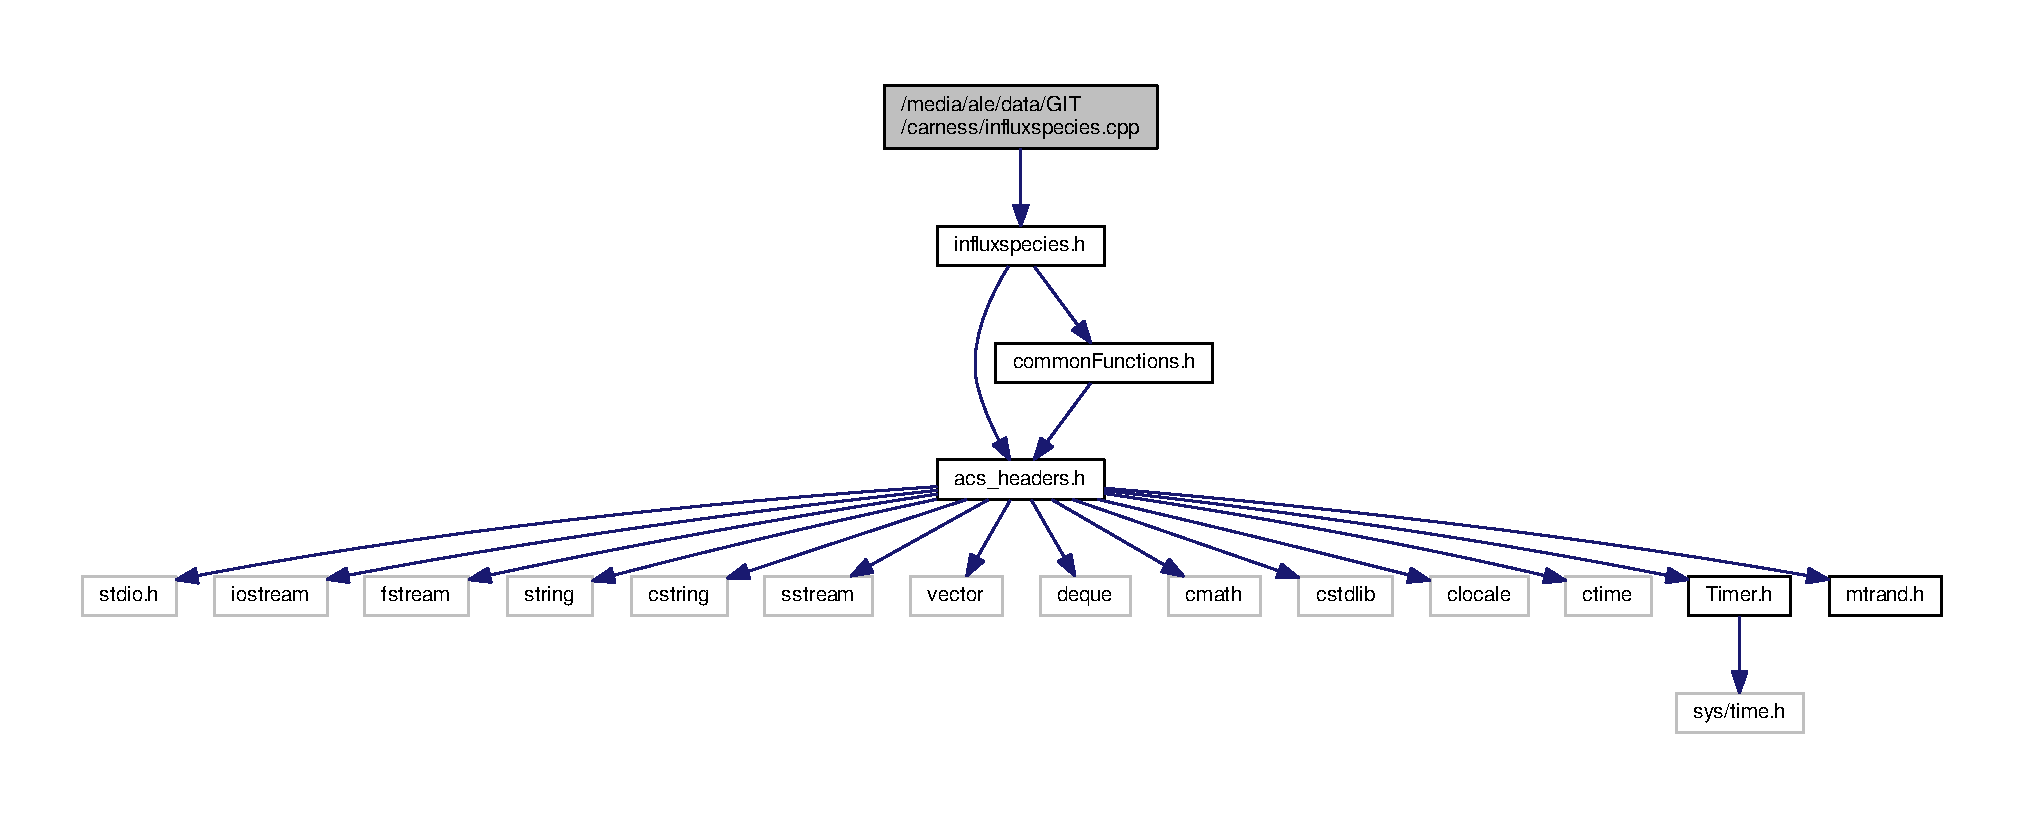
\includegraphics[width=160pt]{a00145}
\end{center}
\end{figure}


Collaboration diagram for M\-T\-Rand\-:\nopagebreak
\begin{figure}[H]
\begin{center}
\leavevmode
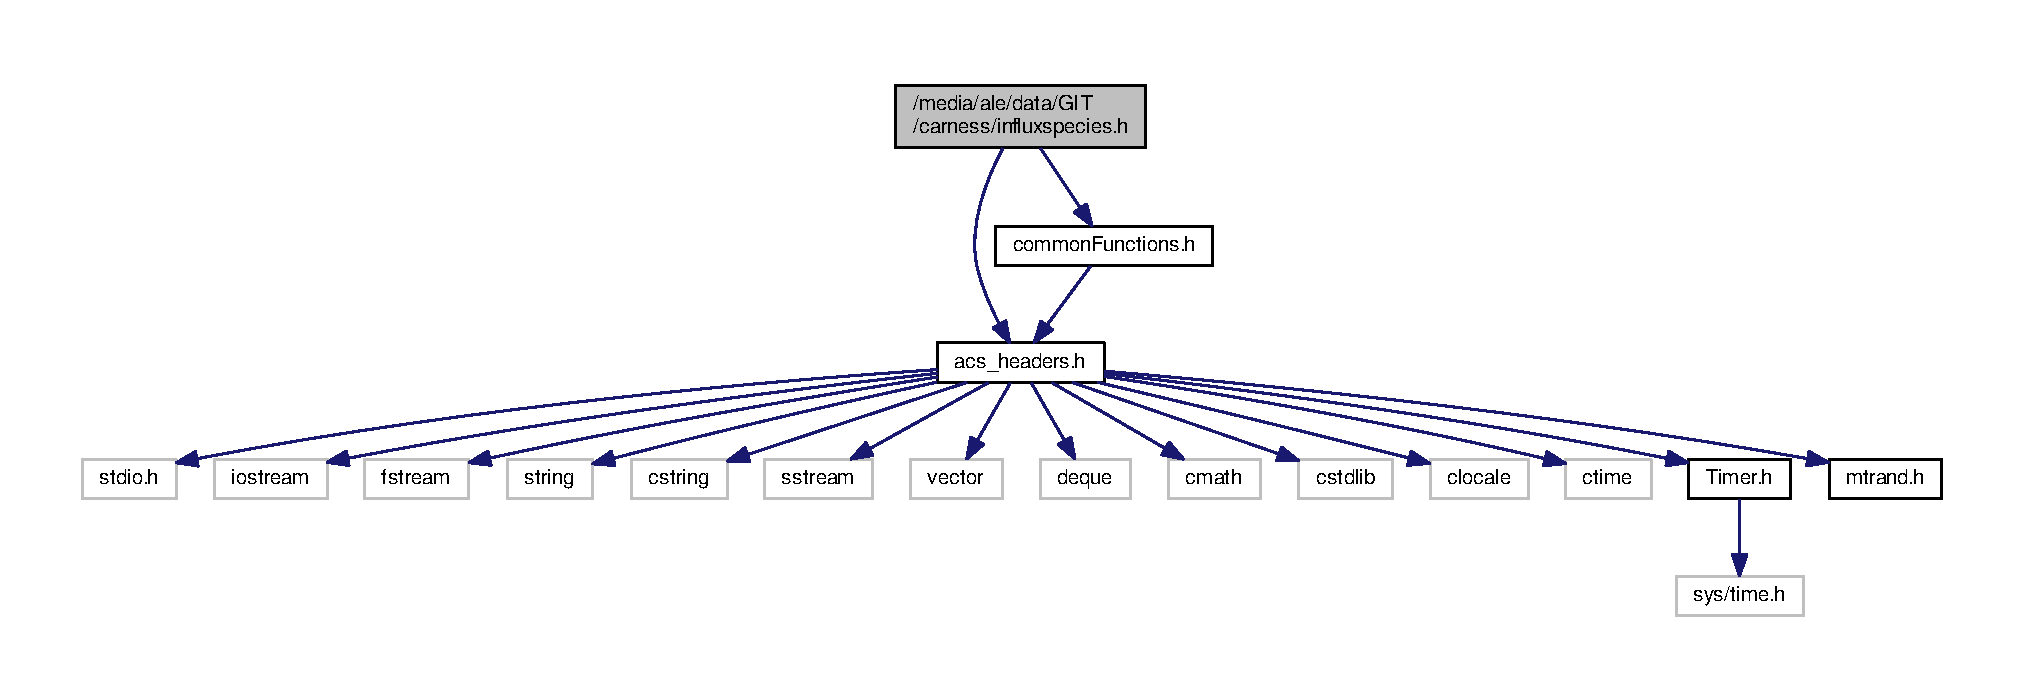
\includegraphics[width=160pt]{a00146}
\end{center}
\end{figure}
\subsection*{Public Member Functions}
\begin{DoxyCompactItemize}
\item 
\hyperlink{a00010_a265dc65546e26073c0d5f8787b045a1d}{M\-T\-Rand} ()
\item 
\hyperlink{a00010_a2c88736896bcbdb54bcdd7a0026720d5}{M\-T\-Rand} (unsigned long \hyperlink{a00013_a0c57076fe30358e0700a7ce1baa0ea27}{seed})
\item 
\hyperlink{a00010_a6075a3beacdfb8e4cf48d9fb56cc193a}{M\-T\-Rand} (const unsigned long $\ast$\hyperlink{a00013_a0c57076fe30358e0700a7ce1baa0ea27}{seed}, int \hyperlink{a00056_ae113ea7f9e515a12ac4b5595c6faf61e}{size})
\item 
\hyperlink{a00010_a8c276546a41ae350dc9efc5e9c10a261}{$\sim$\-M\-T\-Rand} ()
\item 
double \hyperlink{a00010_abbb87a08d622d58fdee0eea4cb5471a0}{operator()} ()
\end{DoxyCompactItemize}
\subsection*{Additional Inherited Members}


\subsection{Detailed Description}


Definition at line 97 of file mtrand.\-h.



\subsection{Constructor \& Destructor Documentation}
\hypertarget{a00010_a265dc65546e26073c0d5f8787b045a1d}{\index{M\-T\-Rand@{M\-T\-Rand}!M\-T\-Rand@{M\-T\-Rand}}
\index{M\-T\-Rand@{M\-T\-Rand}!MTRand@{M\-T\-Rand}}
\subsubsection[{M\-T\-Rand}]{\setlength{\rightskip}{0pt plus 5cm}M\-T\-Rand\-::\-M\-T\-Rand (
\begin{DoxyParamCaption}
{}
\end{DoxyParamCaption}
)\hspace{0.3cm}{\ttfamily [inline]}}}\label{a00010_a265dc65546e26073c0d5f8787b045a1d}


Definition at line 99 of file mtrand.\-h.

\hypertarget{a00010_a2c88736896bcbdb54bcdd7a0026720d5}{\index{M\-T\-Rand@{M\-T\-Rand}!M\-T\-Rand@{M\-T\-Rand}}
\index{M\-T\-Rand@{M\-T\-Rand}!MTRand@{M\-T\-Rand}}
\subsubsection[{M\-T\-Rand}]{\setlength{\rightskip}{0pt plus 5cm}M\-T\-Rand\-::\-M\-T\-Rand (
\begin{DoxyParamCaption}
\item[{unsigned long}]{seed}
\end{DoxyParamCaption}
)\hspace{0.3cm}{\ttfamily [inline]}}}\label{a00010_a2c88736896bcbdb54bcdd7a0026720d5}


Definition at line 100 of file mtrand.\-h.

\hypertarget{a00010_a6075a3beacdfb8e4cf48d9fb56cc193a}{\index{M\-T\-Rand@{M\-T\-Rand}!M\-T\-Rand@{M\-T\-Rand}}
\index{M\-T\-Rand@{M\-T\-Rand}!MTRand@{M\-T\-Rand}}
\subsubsection[{M\-T\-Rand}]{\setlength{\rightskip}{0pt plus 5cm}M\-T\-Rand\-::\-M\-T\-Rand (
\begin{DoxyParamCaption}
\item[{const unsigned long $\ast$}]{seed, }
\item[{int}]{size}
\end{DoxyParamCaption}
)\hspace{0.3cm}{\ttfamily [inline]}}}\label{a00010_a6075a3beacdfb8e4cf48d9fb56cc193a}


Definition at line 101 of file mtrand.\-h.

\hypertarget{a00010_a8c276546a41ae350dc9efc5e9c10a261}{\index{M\-T\-Rand@{M\-T\-Rand}!$\sim$\-M\-T\-Rand@{$\sim$\-M\-T\-Rand}}
\index{$\sim$\-M\-T\-Rand@{$\sim$\-M\-T\-Rand}!MTRand@{M\-T\-Rand}}
\subsubsection[{$\sim$\-M\-T\-Rand}]{\setlength{\rightskip}{0pt plus 5cm}M\-T\-Rand\-::$\sim$\-M\-T\-Rand (
\begin{DoxyParamCaption}
{}
\end{DoxyParamCaption}
)\hspace{0.3cm}{\ttfamily [inline]}}}\label{a00010_a8c276546a41ae350dc9efc5e9c10a261}


Definition at line 102 of file mtrand.\-h.



\subsection{Member Function Documentation}
\hypertarget{a00010_abbb87a08d622d58fdee0eea4cb5471a0}{\index{M\-T\-Rand@{M\-T\-Rand}!operator()@{operator()}}
\index{operator()@{operator()}!MTRand@{M\-T\-Rand}}
\subsubsection[{operator()}]{\setlength{\rightskip}{0pt plus 5cm}double M\-T\-Rand\-::operator() (
\begin{DoxyParamCaption}
{}
\end{DoxyParamCaption}
)\hspace{0.3cm}{\ttfamily [inline]}}}\label{a00010_abbb87a08d622d58fdee0eea4cb5471a0}


Definition at line 103 of file mtrand.\-h.



Here is the call graph for this function\-:\nopagebreak
\begin{figure}[H]
\begin{center}
\leavevmode
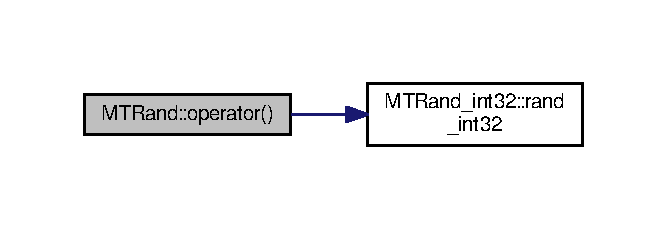
\includegraphics[width=320pt]{a00010_abbb87a08d622d58fdee0eea4cb5471a0_cgraph}
\end{center}
\end{figure}




The documentation for this class was generated from the following file\-:\begin{DoxyCompactItemize}
\item 
/home/ale/\-Documents/\-G\-I\-T/carness/\hyperlink{a00085}{mtrand.\-h}\end{DoxyCompactItemize}

\chapter{Namespace Index}
\section{Namespace List}
Here is a list of all namespaces with brief descriptions\-:\begin{DoxyCompactList}
\item\contentsline{section}{\hyperlink{a00090}{acs\-Attractor\-Analysis} }{\pageref{a00090}}{}
\item\contentsline{section}{\hyperlink{a00091}{acs\-Attractor\-Analysis\-In\-Time} }{\pageref{a00091}}{}
\item\contentsline{section}{\hyperlink{a00092}{acs\-Buffered\-Fluxes} }{\pageref{a00092}}{}
\item\contentsline{section}{\hyperlink{a00093}{acs\-Dyn\-Stat\-In\-Time} }{\pageref{a00093}}{}
\item\contentsline{section}{\hyperlink{a00094}{acs\-From\-Wim2\-Carness} }{\pageref{a00094}}{}
\item\contentsline{section}{\hyperlink{a00095}{acs\-R\-A\-Fanalysis} }{\pageref{a00095}}{}
\item\contentsline{section}{\hyperlink{a00096}{acs\-S\-C\-Canalysis} }{\pageref{a00096}}{}
\item\contentsline{section}{\hyperlink{a00097}{acs\-Species\-Activities} }{\pageref{a00097}}{}
\item\contentsline{section}{\hyperlink{a00098}{acs\-States\-Analysis} }{\pageref{a00098}}{}
\item\contentsline{section}{\hyperlink{a00099}{buffered\-Flux\-Analysis} }{\pageref{a00099}}{}
\item\contentsline{section}{\hyperlink{a00100}{from\-Within2\-Between} }{\pageref{a00100}}{}
\item\contentsline{section}{\hyperlink{a00101}{init} }{\pageref{a00101}}{}
\item\contentsline{section}{\hyperlink{a00102}{lib} }{\pageref{a00102}}{}
\item\contentsline{section}{\hyperlink{a00103}{lib.\-dyn} }{\pageref{a00103}}{}
\item\contentsline{section}{\hyperlink{a00104}{lib.\-dyn.\-dynamics} }{\pageref{a00104}}{}
\item\contentsline{section}{\hyperlink{a00105}{lib.\-graph} }{\pageref{a00105}}{}
\item\contentsline{section}{\hyperlink{a00106}{lib.\-graph.\-network} }{\pageref{a00106}}{}
\item\contentsline{section}{\hyperlink{a00107}{lib.\-graph.\-raf} }{\pageref{a00107}}{}
\item\contentsline{section}{\hyperlink{a00108}{lib.\-I\-O} }{\pageref{a00108}}{}
\item\contentsline{section}{\hyperlink{a00109}{lib.\-I\-O.\-readfiles} }{\pageref{a00109}}{}
\item\contentsline{section}{\hyperlink{a00110}{lib.\-I\-O.\-writefiles} }{\pageref{a00110}}{}
\item\contentsline{section}{\hyperlink{a00111}{main} }{\pageref{a00111}}{}
\item\contentsline{section}{\hyperlink{a00113}{prepare\-New\-Sim} }{\pageref{a00113}}{}
\item\contentsline{section}{\hyperlink{a00115}{reset\-For\-New\-Simulations} }{\pageref{a00115}}{}
\end{DoxyCompactList}

\chapter{Hierarchical Index}
\section{Class Hierarchy}
This inheritance list is sorted roughly, but not completely, alphabetically\-:\begin{DoxyCompactList}
\item \contentsline{section}{catalysis}{\pageref{classcatalysis}}{}
\item \contentsline{section}{common\-Functions}{\pageref{classcommon_functions}}{}
\item \contentsline{section}{environment}{\pageref{classenvironment}}{}
\item \contentsline{section}{gillespie}{\pageref{classgillespie}}{}
\item \contentsline{section}{M\-T\-Rand\-\_\-int32}{\pageref{class_m_t_rand__int32}}{}
\begin{DoxyCompactList}
\item \contentsline{section}{M\-T\-Rand}{\pageref{class_m_t_rand}}{}
\item \contentsline{section}{M\-T\-Rand53}{\pageref{class_m_t_rand53}}{}
\item \contentsline{section}{M\-T\-Rand\-\_\-closed}{\pageref{class_m_t_rand__closed}}{}
\item \contentsline{section}{M\-T\-Rand\-\_\-open}{\pageref{class_m_t_rand__open}}{}
\end{DoxyCompactList}
\item \contentsline{section}{reactions}{\pageref{classreactions}}{}
\item \contentsline{section}{species}{\pageref{classspecies}}{}
\end{DoxyCompactList}

\chapter{Class Index}
\section{Class List}
Here are the classes, structs, unions and interfaces with brief descriptions\-:\begin{DoxyCompactList}
\item\contentsline{section}{\hyperlink{a00006}{catalysis} \\*C\-A\-T\-A\-L\-Y\-S\-I\-S class }{\pageref{a00006}}{}
\item\contentsline{section}{\hyperlink{a00007}{common\-Functions} \\*This class contains all the common function of the system }{\pageref{a00007}}{}
\item\contentsline{section}{\hyperlink{a00008}{environment} \\*Environment class }{\pageref{a00008}}{}
\item\contentsline{section}{\hyperlink{a00009}{gillespie} }{\pageref{a00009}}{}
\item\contentsline{section}{\hyperlink{a00010}{M\-T\-Rand} }{\pageref{a00010}}{}
\item\contentsline{section}{\hyperlink{a00011}{M\-T\-Rand53} }{\pageref{a00011}}{}
\item\contentsline{section}{\hyperlink{a00012}{M\-T\-Rand\-\_\-closed} }{\pageref{a00012}}{}
\item\contentsline{section}{\hyperlink{a00013}{M\-T\-Rand\-\_\-int32} }{\pageref{a00013}}{}
\item\contentsline{section}{\hyperlink{a00014}{M\-T\-Rand\-\_\-open} }{\pageref{a00014}}{}
\item\contentsline{section}{\hyperlink{a00015}{reactions} }{\pageref{a00015}}{}
\item\contentsline{section}{\hyperlink{a00016}{species} \\*This class contains declarations of the species class }{\pageref{a00016}}{}
\end{DoxyCompactList}

\chapter{File Index}
\section{File List}
Here is a list of all files with brief descriptions\-:\begin{DoxyCompactList}
\item\contentsline{section}{/home/ale/\-Documents/\-G\-I\-T/carness/\hyperlink{a00066}{acs\-\_\-headers.\-h} }{\pageref{a00066}}{}
\item\contentsline{section}{/home/ale/\-Documents/\-G\-I\-T/carness/\hyperlink{a00067}{catalysis.\-cpp} }{\pageref{a00067}}{}
\item\contentsline{section}{/home/ale/\-Documents/\-G\-I\-T/carness/\hyperlink{a00068}{catalysis.\-h} }{\pageref{a00068}}{}
\item\contentsline{section}{/home/ale/\-Documents/\-G\-I\-T/carness/\hyperlink{a00069}{common\-Functions.\-cpp} }{\pageref{a00069}}{}
\item\contentsline{section}{/home/ale/\-Documents/\-G\-I\-T/carness/\hyperlink{a00070}{common\-Functions.\-h} }{\pageref{a00070}}{}
\item\contentsline{section}{/home/ale/\-Documents/\-G\-I\-T/carness/\hyperlink{a00079}{environment.\-cpp} }{\pageref{a00079}}{}
\item\contentsline{section}{/home/ale/\-Documents/\-G\-I\-T/carness/\hyperlink{a00080}{environment.\-h} }{\pageref{a00080}}{}
\item\contentsline{section}{/home/ale/\-Documents/\-G\-I\-T/carness/\hyperlink{a00081}{gillespie.\-cpp} }{\pageref{a00081}}{}
\item\contentsline{section}{/home/ale/\-Documents/\-G\-I\-T/carness/\hyperlink{a00082}{gillespie.\-h} }{\pageref{a00082}}{}
\item\contentsline{section}{/home/ale/\-Documents/\-G\-I\-T/carness/\hyperlink{a00083}{main.\-cpp} }{\pageref{a00083}}{}
\item\contentsline{section}{/home/ale/\-Documents/\-G\-I\-T/carness/\hyperlink{a00084}{mtrand.\-cpp} }{\pageref{a00084}}{}
\item\contentsline{section}{/home/ale/\-Documents/\-G\-I\-T/carness/\hyperlink{a00085}{mtrand.\-h} }{\pageref{a00085}}{}
\item\contentsline{section}{/home/ale/\-Documents/\-G\-I\-T/carness/\hyperlink{a00086}{reactions.\-cpp} }{\pageref{a00086}}{}
\item\contentsline{section}{/home/ale/\-Documents/\-G\-I\-T/carness/\hyperlink{a00087}{reactions.\-h} }{\pageref{a00087}}{}
\item\contentsline{section}{/home/ale/\-Documents/\-G\-I\-T/carness/\hyperlink{a00088}{species.\-cpp} }{\pageref{a00088}}{}
\item\contentsline{section}{/home/ale/\-Documents/\-G\-I\-T/carness/\hyperlink{a00089}{species.\-h} }{\pageref{a00089}}{}
\item\contentsline{section}{/home/ale/\-Documents/\-G\-I\-T/carness/\-\_\-analysis/old/\hyperlink{a00017}{all\-Times\-Analysis.\-m} }{\pageref{a00017}}{}
\item\contentsline{section}{/home/ale/\-Documents/\-G\-I\-T/carness/\-\_\-analysis/old/\hyperlink{a00018}{buffered\-Flux\-Analysis.\-py} }{\pageref{a00018}}{}
\item\contentsline{section}{/home/ale/\-Documents/\-G\-I\-T/carness/\-\_\-analysis/old/\hyperlink{a00019}{conc\-Analysis.\-m} }{\pageref{a00019}}{}
\item\contentsline{section}{/home/ale/\-Documents/\-G\-I\-T/carness/\-\_\-analysis/old/\hyperlink{a00020}{from\-Within2\-Between.\-py} }{\pageref{a00020}}{}
\item\contentsline{section}{/home/ale/\-Documents/\-G\-I\-T/carness/\-\_\-analysis/old/\hyperlink{a00021}{garbage\-Search.\-m} }{\pageref{a00021}}{}
\item\contentsline{section}{/home/ale/\-Documents/\-G\-I\-T/carness/\-\_\-analysis/old/\hyperlink{a00022}{general\-Concentration\-Over\-Threshold.\-m} }{\pageref{a00022}}{}
\item\contentsline{section}{/home/ale/\-Documents/\-G\-I\-T/carness/\-\_\-analysis/old/\hyperlink{a00023}{Kill\-Spam.\-m} }{\pageref{a00023}}{}
\item\contentsline{section}{/home/ale/\-Documents/\-G\-I\-T/carness/\-\_\-analysis/old/\hyperlink{a00024}{K\-S\-Search.\-m} }{\pageref{a00024}}{}
\item\contentsline{section}{/home/ale/\-Documents/\-G\-I\-T/carness/\-\_\-analysis/old/\hyperlink{a00025}{K\-S\-Search\-Launcher.\-m} }{\pageref{a00025}}{}
\item\contentsline{section}{/home/ale/\-Documents/\-G\-I\-T/carness/\-\_\-analysis/old/\hyperlink{a00026}{overall\-Stats.\-m} }{\pageref{a00026}}{}
\item\contentsline{section}{/home/ale/\-Documents/\-G\-I\-T/carness/\-\_\-analysis/old/\hyperlink{a00027}{read\-Parameters.\-m} }{\pageref{a00027}}{}
\item\contentsline{section}{/home/ale/\-Documents/\-G\-I\-T/carness/\-\_\-analysis/old/\hyperlink{a00028}{reset\-For\-New\-Simulations.\-py} }{\pageref{a00028}}{}
\item\contentsline{section}{/home/ale/\-Documents/\-G\-I\-T/carness/\-\_\-analysis/old/\hyperlink{a00029}{somma.\-m} }{\pageref{a00029}}{}
\item\contentsline{section}{/home/ale/\-Documents/\-G\-I\-T/carness/\-\_\-analysis/old/\hyperlink{a00030}{stats.\-m} }{\pageref{a00030}}{}
\item\contentsline{section}{/home/ale/\-Documents/\-G\-I\-T/carness/\-\_\-analysis/old/\hyperlink{a00031}{times\-Analysis.\-m} }{\pageref{a00031}}{}
\item\contentsline{section}{/home/ale/\-Documents/\-G\-I\-T/carness/\-\_\-analysis/old/\hyperlink{a00032}{times\-Analysis\-\_\-\-P\-A\-N\-I\-N\-I.\-m} }{\pageref{a00032}}{}
\item\contentsline{section}{/home/ale/\-Documents/\-G\-I\-T/carness/\-\_\-analysis/under\-Development/\hyperlink{a00033}{acs\-Attractor\-Analysis.\-py} }{\pageref{a00033}}{}
\item\contentsline{section}{/home/ale/\-Documents/\-G\-I\-T/carness/\-\_\-analysis/under\-Development/\hyperlink{a00034}{acs\-Attractor\-Analysis\-In\-Time.\-py} }{\pageref{a00034}}{}
\item\contentsline{section}{/home/ale/\-Documents/\-G\-I\-T/carness/\-\_\-analysis/under\-Development/\hyperlink{a00035}{acs\-Buffered\-Fluxes.\-py} }{\pageref{a00035}}{}
\item\contentsline{section}{/home/ale/\-Documents/\-G\-I\-T/carness/\-\_\-analysis/under\-Development/\hyperlink{a00036}{acs\-Dyn\-Stat\-In\-Time.\-py} }{\pageref{a00036}}{}
\item\contentsline{section}{/home/ale/\-Documents/\-G\-I\-T/carness/\-\_\-analysis/under\-Development/\hyperlink{a00037}{acs\-From\-Wim2\-Carness.\-py} }{\pageref{a00037}}{}
\item\contentsline{section}{/home/ale/\-Documents/\-G\-I\-T/carness/\-\_\-analysis/under\-Development/\hyperlink{a00038}{acs\-R\-A\-Fanalysis.\-py} }{\pageref{a00038}}{}
\item\contentsline{section}{/home/ale/\-Documents/\-G\-I\-T/carness/\-\_\-analysis/under\-Development/\hyperlink{a00039}{acs\-S\-C\-Canalysis.\-py} }{\pageref{a00039}}{}
\item\contentsline{section}{/home/ale/\-Documents/\-G\-I\-T/carness/\-\_\-analysis/under\-Development/\hyperlink{a00040}{acs\-Species\-Activities.\-py} }{\pageref{a00040}}{}
\item\contentsline{section}{/home/ale/\-Documents/\-G\-I\-T/carness/\-\_\-analysis/under\-Development/\hyperlink{a00041}{acs\-States\-Analysis.\-py} }{\pageref{a00041}}{}
\item\contentsline{section}{/home/ale/\-Documents/\-G\-I\-T/carness/\-\_\-analysis/under\-Development/\hyperlink{a00042}{init.\-py} }{\pageref{a00042}}{}
\item\contentsline{section}{/home/ale/\-Documents/\-G\-I\-T/carness/\-\_\-analysis/under\-Development/\hyperlink{a00052}{main.\-py} }{\pageref{a00052}}{}
\item\contentsline{section}{/home/ale/\-Documents/\-G\-I\-T/carness/\-\_\-analysis/under\-Development/\hyperlink{a00053}{prepare\-New\-Sim.\-py} }{\pageref{a00053}}{}
\item\contentsline{section}{/home/ale/\-Documents/\-G\-I\-T/carness/\-\_\-analysis/under\-Development/lib/\hyperlink{a00043}{\-\_\-\-\_\-init\-\_\-\-\_\-.\-py} }{\pageref{a00043}}{}
\item\contentsline{section}{/home/ale/\-Documents/\-G\-I\-T/carness/\-\_\-analysis/under\-Development/lib/dyn/\hyperlink{a00044}{\-\_\-\-\_\-init\-\_\-\-\_\-.\-py} }{\pageref{a00044}}{}
\item\contentsline{section}{/home/ale/\-Documents/\-G\-I\-T/carness/\-\_\-analysis/under\-Development/lib/dyn/\hyperlink{a00047}{dynamics.\-py} }{\pageref{a00047}}{}
\item\contentsline{section}{/home/ale/\-Documents/\-G\-I\-T/carness/\-\_\-analysis/under\-Development/lib/graph/\hyperlink{a00045}{\-\_\-\-\_\-init\-\_\-\-\_\-.\-py} }{\pageref{a00045}}{}
\item\contentsline{section}{/home/ale/\-Documents/\-G\-I\-T/carness/\-\_\-analysis/under\-Development/lib/graph/\hyperlink{a00048}{network.\-py} }{\pageref{a00048}}{}
\item\contentsline{section}{/home/ale/\-Documents/\-G\-I\-T/carness/\-\_\-analysis/under\-Development/lib/graph/\hyperlink{a00049}{raf.\-py} }{\pageref{a00049}}{}
\item\contentsline{section}{/home/ale/\-Documents/\-G\-I\-T/carness/\-\_\-analysis/under\-Development/lib/\-I\-O/\hyperlink{a00046}{\-\_\-\-\_\-init\-\_\-\-\_\-.\-py} }{\pageref{a00046}}{}
\item\contentsline{section}{/home/ale/\-Documents/\-G\-I\-T/carness/\-\_\-analysis/under\-Development/lib/\-I\-O/\hyperlink{a00050}{readfiles.\-py} }{\pageref{a00050}}{}
\item\contentsline{section}{/home/ale/\-Documents/\-G\-I\-T/carness/\-\_\-analysis/under\-Development/lib/\-I\-O/\hyperlink{a00051}{writefiles.\-py} }{\pageref{a00051}}{}
\item\contentsline{section}{/home/ale/\-Documents/\-G\-I\-T/carness/\-\_\-matlabinitializator/\hyperlink{a00054}{crea\-\_\-catalizzatori.\-m} }{\pageref{a00054}}{}
\item\contentsline{section}{/home/ale/\-Documents/\-G\-I\-T/carness/\-\_\-matlabinitializator/\hyperlink{a00055}{crea\-\_\-concentrazioni\-\_\-iniziali.\-m} }{\pageref{a00055}}{}
\item\contentsline{section}{/home/ale/\-Documents/\-G\-I\-T/carness/\-\_\-matlabinitializator/\hyperlink{a00056}{crea\-\_\-e\-\_\-controlla\-\_\-i\-\_\-catalizzatori.\-m} }{\pageref{a00056}}{}
\item\contentsline{section}{/home/ale/\-Documents/\-G\-I\-T/carness/\-\_\-matlabinitializator/\hyperlink{a00057}{crea\-\_\-firing\-\_\-disk.\-m} }{\pageref{a00057}}{}
\item\contentsline{section}{/home/ale/\-Documents/\-G\-I\-T/carness/\-\_\-matlabinitializator/\hyperlink{a00058}{crea\-\_\-influx.\-m} }{\pageref{a00058}}{}
\item\contentsline{section}{/home/ale/\-Documents/\-G\-I\-T/carness/\-\_\-matlabinitializator/\hyperlink{a00059}{crea\-\_\-influx\-\_\-semplice.\-m} }{\pageref{a00059}}{}
\item\contentsline{section}{/home/ale/\-Documents/\-G\-I\-T/carness/\-\_\-matlabinitializator/\hyperlink{a00060}{crea\-\_\-tutte\-\_\-le\-\_\-combinazioni\-\_\-di\-\_\-elementi.\-m} }{\pageref{a00060}}{}
\item\contentsline{section}{/home/ale/\-Documents/\-G\-I\-T/carness/\-\_\-matlabinitializator/\hyperlink{a00061}{initial\-\_\-distribution.\-m} }{\pageref{a00061}}{}
\item\contentsline{section}{/home/ale/\-Documents/\-G\-I\-T/carness/\-\_\-matlabinitializator/\hyperlink{a00062}{inizializzatore\-\_\-\-A\-C\-S.\-m} }{\pageref{a00062}}{}
\item\contentsline{section}{/home/ale/\-Documents/\-G\-I\-T/carness/\-\_\-matlabinitializator/\hyperlink{a00063}{lancia\-\_\-acs.\-m} }{\pageref{a00063}}{}
\item\contentsline{section}{/home/ale/\-Documents/\-G\-I\-T/carness/\-\_\-matlabinitializator/\hyperlink{a00064}{lancia\-\_\-inizializzatore\-\_\-acs.\-m} }{\pageref{a00064}}{}
\item\contentsline{section}{/home/ale/\-Documents/\-G\-I\-T/carness/\-\_\-matlabinitializator/\hyperlink{a00065}{start.\-m} }{\pageref{a00065}}{}
\item\contentsline{section}{/home/ale/\-Documents/\-G\-I\-T/carness/\-Debug/\hyperlink{a00071}{catalysis.\-d} }{\pageref{a00071}}{}
\item\contentsline{section}{/home/ale/\-Documents/\-G\-I\-T/carness/\-Debug/\hyperlink{a00072}{common\-Functions.\-d} }{\pageref{a00072}}{}
\item\contentsline{section}{/home/ale/\-Documents/\-G\-I\-T/carness/\-Debug/\hyperlink{a00073}{environment.\-d} }{\pageref{a00073}}{}
\item\contentsline{section}{/home/ale/\-Documents/\-G\-I\-T/carness/\-Debug/\hyperlink{a00074}{gillespie.\-d} }{\pageref{a00074}}{}
\item\contentsline{section}{/home/ale/\-Documents/\-G\-I\-T/carness/\-Debug/\hyperlink{a00075}{main.\-d} }{\pageref{a00075}}{}
\item\contentsline{section}{/home/ale/\-Documents/\-G\-I\-T/carness/\-Debug/\hyperlink{a00076}{mtrand.\-d} }{\pageref{a00076}}{}
\item\contentsline{section}{/home/ale/\-Documents/\-G\-I\-T/carness/\-Debug/\hyperlink{a00077}{reactions.\-d} }{\pageref{a00077}}{}
\item\contentsline{section}{/home/ale/\-Documents/\-G\-I\-T/carness/\-Debug/\hyperlink{a00078}{species.\-d} }{\pageref{a00078}}{}
\end{DoxyCompactList}

\chapter{Namespace Documentation}
\hypertarget{a00096}{\section{/\+Users/alessandrofilisetti/\+Documents/\+G\+I\+T/carness/\+\_\+analysis/python\+Tools/lib/model/species.py File Reference}
\label{a00096}\index{/\+Users/alessandrofilisetti/\+Documents/\+G\+I\+T/carness/\+\_\+analysis/python\+Tools/lib/model/species.\+py@{/\+Users/alessandrofilisetti/\+Documents/\+G\+I\+T/carness/\+\_\+analysis/python\+Tools/lib/model/species.\+py}}
}
\subsection*{Namespaces}
\begin{DoxyCompactItemize}
\item 
 \hyperlink{a00150}{lib.\+model.\+species}
\end{DoxyCompactItemize}
\subsection*{Functions}
\begin{DoxyCompactItemize}
\item 
def \hyperlink{a00150_aaa0ed83b7623b65c77b0d583590219ec}{lib.\+model.\+species.\+create\+Complete\+Species\+Population}
\item 
def \hyperlink{a00150_a1c482d162198854303fbcd154fb1ccbf}{lib.\+model.\+species.\+get\+Tot\+Number\+Of\+Species\+From\+Complete\+Pop}
\item 
def \hyperlink{a00150_a0aab4ec6c7d010b885204f0420072f29}{lib.\+model.\+species.\+create\+File\+Species}
\item 
def \hyperlink{a00150_a13eb7af04a51ec15dd79ef70fadc93f4}{lib.\+model.\+species.\+weighted\+Choice}
\end{DoxyCompactItemize}
\subsection*{Variables}
\begin{DoxyCompactItemize}
\item 
float \hyperlink{a00150_a4a6d118da79b62429ea35b64ef429b11}{lib.\+model.\+species.\+\_\+\+A\+V\+O\+G\+A\+D\+R\+O\+\_\+} = 6.\+022141e23
\end{DoxyCompactItemize}

\hypertarget{a00097}{\section{/\-Users/alessandrofilisetti/\-Documents/\-G\-I\-T/carness/\-\_\-analysis/python\-Tools/lib/visual/graphics.py File Reference}
\label{a00097}\index{/\-Users/alessandrofilisetti/\-Documents/\-G\-I\-T/carness/\-\_\-analysis/python\-Tools/lib/visual/graphics.\-py@{/\-Users/alessandrofilisetti/\-Documents/\-G\-I\-T/carness/\-\_\-analysis/python\-Tools/lib/visual/graphics.\-py}}
}
\subsection*{Namespaces}
\begin{DoxyCompactItemize}
\item 
\hyperlink{a00150}{lib.\-visual.\-graphics}
\end{DoxyCompactItemize}
\subsection*{Functions}
\begin{DoxyCompactItemize}
\item 
def \hyperlink{a00150_aa27c34e948992165c7a98e5ca3605549}{lib.\-visual.\-graphics.\-plot\-\_\-np\-\_\-txt\-\_\-selcols\-\_\-and\-\_\-rows\-\_\-allvarinrows}
\item 
def \hyperlink{a00150_a99e047c066345a973bfbb527e8a91085}{lib.\-visual.\-graphics.\-Plot\-Matrix}
\end{DoxyCompactItemize}
\subsection*{Variables}
\begin{DoxyCompactItemize}
\item 
dictionary \hyperlink{a00150_a3c83ccb4d4d1fcb0ea5f6b8616a1d0df}{lib.\-visual.\-graphics.\-font}
\item 
list \hyperlink{a00150_aae94b6a9df961a260c0fa476e2b4693a}{lib.\-visual.\-graphics.\-colr} = \mbox{[}'\hyperlink{a00110_abf70355c2e58f64c6b18bda1b9bccfd7}{k}','\hyperlink{a00031_ac862e7284527eb913b1351c8bfb8e079}{r}','\hyperlink{a00035_a50b4f3ddde10830a3976c71083aaee3f}{b}','g','\hyperlink{a00035_a6be92348ba85ef257b11d06209e1d7b6}{c}','m','y'\mbox{]}
\end{DoxyCompactItemize}

\hypertarget{a00098}{\section{acs\-Species\-Activities Namespace Reference}
\label{a00098}\index{acs\-Species\-Activities@{acs\-Species\-Activities}}
}
\subsection*{Functions}
\begin{DoxyCompactItemize}
\item 
def \hyperlink{a00098_ac217c91fe2eee20671291adb12bbbbb2}{zero\-Before\-Str\-Num}
\end{DoxyCompactItemize}
\subsection*{Variables}
\begin{DoxyCompactItemize}
\item 
tuple \hyperlink{a00098_aab55eec317b77f6c91a884938a106d3f}{parser}
\item 
tuple \hyperlink{a00098_a2dd673f2cf596c509afd7ad0f3df286b}{args} = parser.\-parse\-\_\-args()
\item 
tuple \hyperlink{a00098_a05f0f829ce4df27678aa19d4e5f10c54}{Str\-Path} = os.\-path.\-abspath(args.\-Str\-Path)
\item 
tuple \hyperlink{a00098_addf4c61c6afe70a2ea39931695ddc36b}{tmp\-Dirs} = sort(os.\-listdir(\hyperlink{a00098_a05f0f829ce4df27678aa19d4e5f10c54}{Str\-Path}))
\item 
int \hyperlink{a00098_a5459c566e6ccdf02747a3c16089a5593}{chemistry} = 1
\item 
string \hyperlink{a00098_ad2a87ed28d0f42525ce49c390f390298}{ndn} = '\-\_\-0\-\_\-new\-\_\-all\-Stat\-Results'
\item 
tuple \hyperlink{a00098_a4fc28291b7f61ee2fa8969fa7a690ba2}{newdir\-All\-Results} = os.\-path.\-join(\hyperlink{a00098_a05f0f829ce4df27678aa19d4e5f10c54}{Str\-Path}, \hyperlink{a00098_ad2a87ed28d0f42525ce49c390f390298}{ndn})
\item 
tuple \hyperlink{a00098_ae77a5ce35739a29f29f9df698d91f1c9}{newdir\-All\-Results\-Inner} = os.\-path.\-join(\hyperlink{a00098_a05f0f829ce4df27678aa19d4e5f10c54}{Str\-Path},'\-\_\-0\-\_\-new\-\_\-all\-Stat\-Results',\hyperlink{a00098_ad2a87ed28d0f42525ce49c390f390298}{ndn})
\item 
tuple \hyperlink{a00098_aa71c948cf1d0699207eafcd30beb394e}{tot\-Dir\-Name} = os.\-path.\-join(\hyperlink{a00098_a05f0f829ce4df27678aa19d4e5f10c54}{Str\-Path},tmp\-Dir)
\item 
tuple \hyperlink{a00098_a2c1728d3ec9815ec7cf41653e953524c}{res\-Dir\-Path} = os.\-path.\-abspath(os.\-path.\-join(\char`\"{}./\char`\"{}, \char`\"{}res\char`\"{}))
\item 
tuple \hyperlink{a00098_acceae37ca98ccf6dc25c9f538fda386f}{number\-Of\-Gen} = len(glob.\-glob(os.\-path.\-join(\hyperlink{a00098_a2c1728d3ec9815ec7cf41653e953524c}{res\-Dir\-Path},'times\-\_\-$\ast$')))
\item 
string \hyperlink{a00098_aceab16acbf85893dcacfcfd921c9da12}{tmp\-Species\-Stats\-Summary\-Name} = 'species\-Stats\-Summary\-\_\-'
\item 
tuple \hyperlink{a00098_a57b362cf15dda461a59c719a92177c3a}{tmp\-Species\-Stats\-Summary\-Name\-F\-I\-D} = open(\hyperlink{a00098_aceab16acbf85893dcacfcfd921c9da12}{tmp\-Species\-Stats\-Summary\-Name}, 'w')
\item 
string \hyperlink{a00098_a81ab8133517c53adfcdf8129e24cf5d0}{tmp\-Str} = '\textbackslash{}n-\/-\/-\/-\/-\/-\/-\/ C\-H\-E\-M\-I\-S\-T\-R\-Y '
\item 
tuple \hyperlink{a00098_ac53f52471f3cf1ef18465a07dc930dff}{str\-Zeros} = \hyperlink{a00098_ac217c91fe2eee20671291adb12bbbbb2}{zero\-Before\-Str\-Num}(ngen, \hyperlink{a00098_acceae37ca98ccf6dc25c9f538fda386f}{number\-Of\-Gen})
\item 
string \hyperlink{a00098_a78927c369e0fe9deb29777c699af346f}{str\-Species\-Zero} = 'species\-\_\-'
\item 
tuple \hyperlink{a00098_a2f73b228eca2d5d0e45f781ccc21b253}{species\-Files\-Zero} = sorted(glob.\-glob(os.\-path.\-join(\hyperlink{a00098_a2c1728d3ec9815ec7cf41653e953524c}{res\-Dir\-Path},\hyperlink{a00098_a78927c369e0fe9deb29777c699af346f}{str\-Species\-Zero})))
\item 
string \hyperlink{a00098_a7ad6c119fecb41b02823a95f334daa4c}{str\-Species} = 'species\-\_\-'
\item 
tuple \hyperlink{a00098_a7e3b3a6b0c9305e60758bf5d44e7b0f6}{species\-Files} = sorted(glob.\-glob(os.\-path.\-join(\hyperlink{a00098_a2c1728d3ec9815ec7cf41653e953524c}{res\-Dir\-Path},\hyperlink{a00098_a7ad6c119fecb41b02823a95f334daa4c}{str\-Species})))
\item 
list \hyperlink{a00098_ac7070acb2aaeb8965c57e81b6308ddd5}{lastfilespecies} = \hyperlink{a00098_a7e3b3a6b0c9305e60758bf5d44e7b0f6}{species\-Files}\mbox{[}-\/1\mbox{]}
\item 
tuple \hyperlink{a00098_a240d5b3cd72043528f4b674a8ba00a33}{fid\-Species} = open(\hyperlink{a00098_ac7070acb2aaeb8965c57e81b6308ddd5}{lastfilespecies}, '\hyperlink{a00024_ac862e7284527eb913b1351c8bfb8e079}{r}')
\item 
list \hyperlink{a00098_a50a8f7f4bae0fd037961d91206f5178c}{seq} = \mbox{[}$\,$\mbox{]}
\item 
tuple \hyperlink{a00098_a6afffdd046bbc3bc4fbee34b561fcae5}{counters} = np.\-zeros((n\-Species,3))
\item 
string \hyperlink{a00098_ab59af27efe5462ef13ae45fd7330d0b3}{str\-Rct\-Par} = 'reactions\-\_\-parameters\-\_\-'
\item 
tuple \hyperlink{a00098_a64247b23c199d0b0d0d60f02ec8682e3}{fid\-Rct\-Par} = open(\hyperlink{a00098_ab59af27efe5462ef13ae45fd7330d0b3}{str\-Rct\-Par}, '\hyperlink{a00024_ac862e7284527eb913b1351c8bfb8e079}{r}')
\item 
tuple \hyperlink{a00098_abdc37f53b75138949fbbe9f9e42f1e6f}{rct\-Type} = int(tmp\-Rct\-Type)
\item 
tuple \hyperlink{a00098_a721a520fa04949579e29cb858dc00bf0}{cat} = int(tmp\-Cat)
\item 
tuple \hyperlink{a00098_a4ffac9566fa24baa2b27ccd97f9ffe1e}{S1} = int(tmp\-S1)
\item 
tuple \hyperlink{a00098_a3b95f66d848ccbac2740be2878b2499b}{S2} = int(tmp\-S2)
\item 
tuple \hyperlink{a00098_a654d2a657cf4b354b3791a8b2de3d74e}{S3} = int(tmp\-S3)
\item 
string \hyperlink{a00098_a23844a8104156ee329f8c957f11490f4}{tmp\-File\-Name} = 'species\-Stats\-\_\-'
\item 
tuple \hyperlink{a00098_addb867cf8533f2e18682c49f08f47bba}{tmp\-File\-Name\-F\-I\-D} = open(\hyperlink{a00098_a23844a8104156ee329f8c957f11490f4}{tmp\-File\-Name}, 'w')
\item 
int \hyperlink{a00098_a8102909ea2c113190493bd581f17ba18}{I\-D} = 0
\end{DoxyCompactItemize}


\subsection{Function Documentation}
\hypertarget{a00098_ac217c91fe2eee20671291adb12bbbbb2}{\index{acs\-Species\-Activities@{acs\-Species\-Activities}!zero\-Before\-Str\-Num@{zero\-Before\-Str\-Num}}
\index{zero\-Before\-Str\-Num@{zero\-Before\-Str\-Num}!acsSpeciesActivities@{acs\-Species\-Activities}}
\subsubsection[{zero\-Before\-Str\-Num}]{\setlength{\rightskip}{0pt plus 5cm}def acs\-Species\-Activities.\-zero\-Before\-Str\-Num (
\begin{DoxyParamCaption}
\item[{}]{tmpl, }
\item[{}]{tmp\-L}
\end{DoxyParamCaption}
)}}\label{a00098_ac217c91fe2eee20671291adb12bbbbb2}


Definition at line 20 of file acs\-Species\-Activities.\-py.



\subsection{Variable Documentation}
\hypertarget{a00098_a2dd673f2cf596c509afd7ad0f3df286b}{\index{acs\-Species\-Activities@{acs\-Species\-Activities}!args@{args}}
\index{args@{args}!acsSpeciesActivities@{acs\-Species\-Activities}}
\subsubsection[{args}]{\setlength{\rightskip}{0pt plus 5cm}tuple acs\-Species\-Activities.\-args = parser.\-parse\-\_\-args()}}\label{a00098_a2dd673f2cf596c509afd7ad0f3df286b}


Definition at line 34 of file acs\-Species\-Activities.\-py.

\hypertarget{a00098_a721a520fa04949579e29cb858dc00bf0}{\index{acs\-Species\-Activities@{acs\-Species\-Activities}!cat@{cat}}
\index{cat@{cat}!acsSpeciesActivities@{acs\-Species\-Activities}}
\subsubsection[{cat}]{\setlength{\rightskip}{0pt plus 5cm}tuple acs\-Species\-Activities.\-cat = int(tmp\-Cat)}}\label{a00098_a721a520fa04949579e29cb858dc00bf0}


Definition at line 131 of file acs\-Species\-Activities.\-py.

\hypertarget{a00098_a5459c566e6ccdf02747a3c16089a5593}{\index{acs\-Species\-Activities@{acs\-Species\-Activities}!chemistry@{chemistry}}
\index{chemistry@{chemistry}!acsSpeciesActivities@{acs\-Species\-Activities}}
\subsubsection[{chemistry}]{\setlength{\rightskip}{0pt plus 5cm}int acs\-Species\-Activities.\-chemistry = 1}}\label{a00098_a5459c566e6ccdf02747a3c16089a5593}


Definition at line 44 of file acs\-Species\-Activities.\-py.

\hypertarget{a00098_a6afffdd046bbc3bc4fbee34b561fcae5}{\index{acs\-Species\-Activities@{acs\-Species\-Activities}!counters@{counters}}
\index{counters@{counters}!acsSpeciesActivities@{acs\-Species\-Activities}}
\subsubsection[{counters}]{\setlength{\rightskip}{0pt plus 5cm}tuple acs\-Species\-Activities.\-counters = np.\-zeros((n\-Species,3))}}\label{a00098_a6afffdd046bbc3bc4fbee34b561fcae5}


Definition at line 117 of file acs\-Species\-Activities.\-py.

\hypertarget{a00098_a64247b23c199d0b0d0d60f02ec8682e3}{\index{acs\-Species\-Activities@{acs\-Species\-Activities}!fid\-Rct\-Par@{fid\-Rct\-Par}}
\index{fid\-Rct\-Par@{fid\-Rct\-Par}!acsSpeciesActivities@{acs\-Species\-Activities}}
\subsubsection[{fid\-Rct\-Par}]{\setlength{\rightskip}{0pt plus 5cm}tuple acs\-Species\-Activities.\-fid\-Rct\-Par = open({\bf str\-Rct\-Par}, '{\bf r}')}}\label{a00098_a64247b23c199d0b0d0d60f02ec8682e3}


Definition at line 123 of file acs\-Species\-Activities.\-py.

\hypertarget{a00098_a240d5b3cd72043528f4b674a8ba00a33}{\index{acs\-Species\-Activities@{acs\-Species\-Activities}!fid\-Species@{fid\-Species}}
\index{fid\-Species@{fid\-Species}!acsSpeciesActivities@{acs\-Species\-Activities}}
\subsubsection[{fid\-Species}]{\setlength{\rightskip}{0pt plus 5cm}tuple acs\-Species\-Activities.\-fid\-Species = open({\bf lastfilespecies}, '{\bf r}')}}\label{a00098_a240d5b3cd72043528f4b674a8ba00a33}


Definition at line 106 of file acs\-Species\-Activities.\-py.

\hypertarget{a00098_a8102909ea2c113190493bd581f17ba18}{\index{acs\-Species\-Activities@{acs\-Species\-Activities}!I\-D@{I\-D}}
\index{I\-D@{I\-D}!acsSpeciesActivities@{acs\-Species\-Activities}}
\subsubsection[{I\-D}]{\setlength{\rightskip}{0pt plus 5cm}int acs\-Species\-Activities.\-I\-D = 0}}\label{a00098_a8102909ea2c113190493bd581f17ba18}


Definition at line 163 of file acs\-Species\-Activities.\-py.

\hypertarget{a00098_ac7070acb2aaeb8965c57e81b6308ddd5}{\index{acs\-Species\-Activities@{acs\-Species\-Activities}!lastfilespecies@{lastfilespecies}}
\index{lastfilespecies@{lastfilespecies}!acsSpeciesActivities@{acs\-Species\-Activities}}
\subsubsection[{lastfilespecies}]{\setlength{\rightskip}{0pt plus 5cm}list acs\-Species\-Activities.\-lastfilespecies = {\bf species\-Files}\mbox{[}-\/1\mbox{]}}}\label{a00098_ac7070acb2aaeb8965c57e81b6308ddd5}


Definition at line 102 of file acs\-Species\-Activities.\-py.

\hypertarget{a00098_ad2a87ed28d0f42525ce49c390f390298}{\index{acs\-Species\-Activities@{acs\-Species\-Activities}!ndn@{ndn}}
\index{ndn@{ndn}!acsSpeciesActivities@{acs\-Species\-Activities}}
\subsubsection[{ndn}]{\setlength{\rightskip}{0pt plus 5cm}string acs\-Species\-Activities.\-ndn = '\-\_\-0\-\_\-new\-\_\-all\-Stat\-Results'}}\label{a00098_ad2a87ed28d0f42525ce49c390f390298}


Definition at line 47 of file acs\-Species\-Activities.\-py.

\hypertarget{a00098_a4fc28291b7f61ee2fa8969fa7a690ba2}{\index{acs\-Species\-Activities@{acs\-Species\-Activities}!newdir\-All\-Results@{newdir\-All\-Results}}
\index{newdir\-All\-Results@{newdir\-All\-Results}!acsSpeciesActivities@{acs\-Species\-Activities}}
\subsubsection[{newdir\-All\-Results}]{\setlength{\rightskip}{0pt plus 5cm}tuple acs\-Species\-Activities.\-newdir\-All\-Results = os.\-path.\-join({\bf Str\-Path}, {\bf ndn})}}\label{a00098_a4fc28291b7f61ee2fa8969fa7a690ba2}


Definition at line 48 of file acs\-Species\-Activities.\-py.

\hypertarget{a00098_ae77a5ce35739a29f29f9df698d91f1c9}{\index{acs\-Species\-Activities@{acs\-Species\-Activities}!newdir\-All\-Results\-Inner@{newdir\-All\-Results\-Inner}}
\index{newdir\-All\-Results\-Inner@{newdir\-All\-Results\-Inner}!acsSpeciesActivities@{acs\-Species\-Activities}}
\subsubsection[{newdir\-All\-Results\-Inner}]{\setlength{\rightskip}{0pt plus 5cm}tuple acs\-Species\-Activities.\-newdir\-All\-Results\-Inner = os.\-path.\-join({\bf Str\-Path},'\-\_\-0\-\_\-new\-\_\-all\-Stat\-Results',{\bf ndn})}}\label{a00098_ae77a5ce35739a29f29f9df698d91f1c9}


Definition at line 56 of file acs\-Species\-Activities.\-py.

\hypertarget{a00098_acceae37ca98ccf6dc25c9f538fda386f}{\index{acs\-Species\-Activities@{acs\-Species\-Activities}!number\-Of\-Gen@{number\-Of\-Gen}}
\index{number\-Of\-Gen@{number\-Of\-Gen}!acsSpeciesActivities@{acs\-Species\-Activities}}
\subsubsection[{number\-Of\-Gen}]{\setlength{\rightskip}{0pt plus 5cm}tuple acs\-Species\-Activities.\-number\-Of\-Gen = len(glob.\-glob(os.\-path.\-join({\bf res\-Dir\-Path},'times\-\_\-$\ast$')))}}\label{a00098_acceae37ca98ccf6dc25c9f538fda386f}


Definition at line 75 of file acs\-Species\-Activities.\-py.

\hypertarget{a00098_aab55eec317b77f6c91a884938a106d3f}{\index{acs\-Species\-Activities@{acs\-Species\-Activities}!parser@{parser}}
\index{parser@{parser}!acsSpeciesActivities@{acs\-Species\-Activities}}
\subsubsection[{parser}]{\setlength{\rightskip}{0pt plus 5cm}tuple acs\-Species\-Activities.\-parser}}\label{a00098_aab55eec317b77f6c91a884938a106d3f}
{\bfseries Initial value\-:}
\begin{DoxyCode}
1 = ArgumentParser(
2                                 description=\textcolor{stringliteral}{'Function to evaluate the activity of each species during the
       simulation, \(\backslash\)}
3 \textcolor{stringliteral}{                                catalyst substrate product or nothing. Moreover the script recognize all
       those molecules functioning as hub'}
4                                 , epilog=\textcolor{stringliteral}{'''File with angle trajectories are created. '''})
\end{DoxyCode}


Definition at line 29 of file acs\-Species\-Activities.\-py.

\hypertarget{a00098_abdc37f53b75138949fbbe9f9e42f1e6f}{\index{acs\-Species\-Activities@{acs\-Species\-Activities}!rct\-Type@{rct\-Type}}
\index{rct\-Type@{rct\-Type}!acsSpeciesActivities@{acs\-Species\-Activities}}
\subsubsection[{rct\-Type}]{\setlength{\rightskip}{0pt plus 5cm}tuple acs\-Species\-Activities.\-rct\-Type = int(tmp\-Rct\-Type)}}\label{a00098_abdc37f53b75138949fbbe9f9e42f1e6f}


Definition at line 130 of file acs\-Species\-Activities.\-py.

\hypertarget{a00098_a2c1728d3ec9815ec7cf41653e953524c}{\index{acs\-Species\-Activities@{acs\-Species\-Activities}!res\-Dir\-Path@{res\-Dir\-Path}}
\index{res\-Dir\-Path@{res\-Dir\-Path}!acsSpeciesActivities@{acs\-Species\-Activities}}
\subsubsection[{res\-Dir\-Path}]{\setlength{\rightskip}{0pt plus 5cm}tuple acs\-Species\-Activities.\-res\-Dir\-Path = os.\-path.\-abspath(os.\-path.\-join(\char`\"{}./\char`\"{}, \char`\"{}res\char`\"{}))}}\label{a00098_a2c1728d3ec9815ec7cf41653e953524c}


Definition at line 69 of file acs\-Species\-Activities.\-py.

\hypertarget{a00098_a4ffac9566fa24baa2b27ccd97f9ffe1e}{\index{acs\-Species\-Activities@{acs\-Species\-Activities}!S1@{S1}}
\index{S1@{S1}!acsSpeciesActivities@{acs\-Species\-Activities}}
\subsubsection[{S1}]{\setlength{\rightskip}{0pt plus 5cm}tuple acs\-Species\-Activities.\-S1 = int(tmp\-S1)}}\label{a00098_a4ffac9566fa24baa2b27ccd97f9ffe1e}


Definition at line 132 of file acs\-Species\-Activities.\-py.

\hypertarget{a00098_a3b95f66d848ccbac2740be2878b2499b}{\index{acs\-Species\-Activities@{acs\-Species\-Activities}!S2@{S2}}
\index{S2@{S2}!acsSpeciesActivities@{acs\-Species\-Activities}}
\subsubsection[{S2}]{\setlength{\rightskip}{0pt plus 5cm}tuple acs\-Species\-Activities.\-S2 = int(tmp\-S2)}}\label{a00098_a3b95f66d848ccbac2740be2878b2499b}


Definition at line 133 of file acs\-Species\-Activities.\-py.

\hypertarget{a00098_a654d2a657cf4b354b3791a8b2de3d74e}{\index{acs\-Species\-Activities@{acs\-Species\-Activities}!S3@{S3}}
\index{S3@{S3}!acsSpeciesActivities@{acs\-Species\-Activities}}
\subsubsection[{S3}]{\setlength{\rightskip}{0pt plus 5cm}tuple acs\-Species\-Activities.\-S3 = int(tmp\-S3)}}\label{a00098_a654d2a657cf4b354b3791a8b2de3d74e}


Definition at line 134 of file acs\-Species\-Activities.\-py.

\hypertarget{a00098_a50a8f7f4bae0fd037961d91206f5178c}{\index{acs\-Species\-Activities@{acs\-Species\-Activities}!seq@{seq}}
\index{seq@{seq}!acsSpeciesActivities@{acs\-Species\-Activities}}
\subsubsection[{seq}]{\setlength{\rightskip}{0pt plus 5cm}list acs\-Species\-Activities.\-seq = \mbox{[}$\,$\mbox{]}}}\label{a00098_a50a8f7f4bae0fd037961d91206f5178c}


Definition at line 110 of file acs\-Species\-Activities.\-py.

\hypertarget{a00098_a7e3b3a6b0c9305e60758bf5d44e7b0f6}{\index{acs\-Species\-Activities@{acs\-Species\-Activities}!species\-Files@{species\-Files}}
\index{species\-Files@{species\-Files}!acsSpeciesActivities@{acs\-Species\-Activities}}
\subsubsection[{species\-Files}]{\setlength{\rightskip}{0pt plus 5cm}tuple acs\-Species\-Activities.\-species\-Files = sorted(glob.\-glob(os.\-path.\-join({\bf res\-Dir\-Path},{\bf str\-Species})))}}\label{a00098_a7e3b3a6b0c9305e60758bf5d44e7b0f6}


Definition at line 99 of file acs\-Species\-Activities.\-py.

\hypertarget{a00098_a2f73b228eca2d5d0e45f781ccc21b253}{\index{acs\-Species\-Activities@{acs\-Species\-Activities}!species\-Files\-Zero@{species\-Files\-Zero}}
\index{species\-Files\-Zero@{species\-Files\-Zero}!acsSpeciesActivities@{acs\-Species\-Activities}}
\subsubsection[{species\-Files\-Zero}]{\setlength{\rightskip}{0pt plus 5cm}tuple acs\-Species\-Activities.\-species\-Files\-Zero = sorted(glob.\-glob(os.\-path.\-join({\bf res\-Dir\-Path},{\bf str\-Species\-Zero})))}}\label{a00098_a2f73b228eca2d5d0e45f781ccc21b253}


Definition at line 94 of file acs\-Species\-Activities.\-py.

\hypertarget{a00098_a05f0f829ce4df27678aa19d4e5f10c54}{\index{acs\-Species\-Activities@{acs\-Species\-Activities}!Str\-Path@{Str\-Path}}
\index{Str\-Path@{Str\-Path}!acsSpeciesActivities@{acs\-Species\-Activities}}
\subsubsection[{Str\-Path}]{\setlength{\rightskip}{0pt plus 5cm}tuple acs\-Species\-Activities.\-Str\-Path = os.\-path.\-abspath(args.\-Str\-Path)}}\label{a00098_a05f0f829ce4df27678aa19d4e5f10c54}


Definition at line 37 of file acs\-Species\-Activities.\-py.

\hypertarget{a00098_ab59af27efe5462ef13ae45fd7330d0b3}{\index{acs\-Species\-Activities@{acs\-Species\-Activities}!str\-Rct\-Par@{str\-Rct\-Par}}
\index{str\-Rct\-Par@{str\-Rct\-Par}!acsSpeciesActivities@{acs\-Species\-Activities}}
\subsubsection[{str\-Rct\-Par}]{\setlength{\rightskip}{0pt plus 5cm}string acs\-Species\-Activities.\-str\-Rct\-Par = 'reactions\-\_\-parameters\-\_\-'}}\label{a00098_ab59af27efe5462ef13ae45fd7330d0b3}


Definition at line 119 of file acs\-Species\-Activities.\-py.

\hypertarget{a00098_a7ad6c119fecb41b02823a95f334daa4c}{\index{acs\-Species\-Activities@{acs\-Species\-Activities}!str\-Species@{str\-Species}}
\index{str\-Species@{str\-Species}!acsSpeciesActivities@{acs\-Species\-Activities}}
\subsubsection[{str\-Species}]{\setlength{\rightskip}{0pt plus 5cm}string acs\-Species\-Activities.\-str\-Species = 'species\-\_\-'}}\label{a00098_a7ad6c119fecb41b02823a95f334daa4c}


Definition at line 96 of file acs\-Species\-Activities.\-py.

\hypertarget{a00098_a78927c369e0fe9deb29777c699af346f}{\index{acs\-Species\-Activities@{acs\-Species\-Activities}!str\-Species\-Zero@{str\-Species\-Zero}}
\index{str\-Species\-Zero@{str\-Species\-Zero}!acsSpeciesActivities@{acs\-Species\-Activities}}
\subsubsection[{str\-Species\-Zero}]{\setlength{\rightskip}{0pt plus 5cm}string acs\-Species\-Activities.\-str\-Species\-Zero = 'species\-\_\-'}}\label{a00098_a78927c369e0fe9deb29777c699af346f}


Definition at line 93 of file acs\-Species\-Activities.\-py.

\hypertarget{a00098_ac53f52471f3cf1ef18465a07dc930dff}{\index{acs\-Species\-Activities@{acs\-Species\-Activities}!str\-Zeros@{str\-Zeros}}
\index{str\-Zeros@{str\-Zeros}!acsSpeciesActivities@{acs\-Species\-Activities}}
\subsubsection[{str\-Zeros}]{\setlength{\rightskip}{0pt plus 5cm}tuple acs\-Species\-Activities.\-str\-Zeros = {\bf zero\-Before\-Str\-Num}(ngen, {\bf number\-Of\-Gen})}}\label{a00098_ac53f52471f3cf1ef18465a07dc930dff}


Definition at line 91 of file acs\-Species\-Activities.\-py.

\hypertarget{a00098_addf4c61c6afe70a2ea39931695ddc36b}{\index{acs\-Species\-Activities@{acs\-Species\-Activities}!tmp\-Dirs@{tmp\-Dirs}}
\index{tmp\-Dirs@{tmp\-Dirs}!acsSpeciesActivities@{acs\-Species\-Activities}}
\subsubsection[{tmp\-Dirs}]{\setlength{\rightskip}{0pt plus 5cm}tuple acs\-Species\-Activities.\-tmp\-Dirs = sort(os.\-listdir({\bf Str\-Path}))}}\label{a00098_addf4c61c6afe70a2ea39931695ddc36b}


Definition at line 39 of file acs\-Species\-Activities.\-py.

\hypertarget{a00098_a23844a8104156ee329f8c957f11490f4}{\index{acs\-Species\-Activities@{acs\-Species\-Activities}!tmp\-File\-Name@{tmp\-File\-Name}}
\index{tmp\-File\-Name@{tmp\-File\-Name}!acsSpeciesActivities@{acs\-Species\-Activities}}
\subsubsection[{tmp\-File\-Name}]{\setlength{\rightskip}{0pt plus 5cm}string acs\-Species\-Activities.\-tmp\-File\-Name = 'species\-Stats\-\_\-'}}\label{a00098_a23844a8104156ee329f8c957f11490f4}


Definition at line 160 of file acs\-Species\-Activities.\-py.

\hypertarget{a00098_addb867cf8533f2e18682c49f08f47bba}{\index{acs\-Species\-Activities@{acs\-Species\-Activities}!tmp\-File\-Name\-F\-I\-D@{tmp\-File\-Name\-F\-I\-D}}
\index{tmp\-File\-Name\-F\-I\-D@{tmp\-File\-Name\-F\-I\-D}!acsSpeciesActivities@{acs\-Species\-Activities}}
\subsubsection[{tmp\-File\-Name\-F\-I\-D}]{\setlength{\rightskip}{0pt plus 5cm}tuple acs\-Species\-Activities.\-tmp\-File\-Name\-F\-I\-D = open({\bf tmp\-File\-Name}, 'w')}}\label{a00098_addb867cf8533f2e18682c49f08f47bba}


Definition at line 162 of file acs\-Species\-Activities.\-py.

\hypertarget{a00098_aceab16acbf85893dcacfcfd921c9da12}{\index{acs\-Species\-Activities@{acs\-Species\-Activities}!tmp\-Species\-Stats\-Summary\-Name@{tmp\-Species\-Stats\-Summary\-Name}}
\index{tmp\-Species\-Stats\-Summary\-Name@{tmp\-Species\-Stats\-Summary\-Name}!acsSpeciesActivities@{acs\-Species\-Activities}}
\subsubsection[{tmp\-Species\-Stats\-Summary\-Name}]{\setlength{\rightskip}{0pt plus 5cm}string acs\-Species\-Activities.\-tmp\-Species\-Stats\-Summary\-Name = 'species\-Stats\-Summary\-\_\-'}}\label{a00098_aceab16acbf85893dcacfcfd921c9da12}


Definition at line 80 of file acs\-Species\-Activities.\-py.

\hypertarget{a00098_a57b362cf15dda461a59c719a92177c3a}{\index{acs\-Species\-Activities@{acs\-Species\-Activities}!tmp\-Species\-Stats\-Summary\-Name\-F\-I\-D@{tmp\-Species\-Stats\-Summary\-Name\-F\-I\-D}}
\index{tmp\-Species\-Stats\-Summary\-Name\-F\-I\-D@{tmp\-Species\-Stats\-Summary\-Name\-F\-I\-D}!acsSpeciesActivities@{acs\-Species\-Activities}}
\subsubsection[{tmp\-Species\-Stats\-Summary\-Name\-F\-I\-D}]{\setlength{\rightskip}{0pt plus 5cm}tuple acs\-Species\-Activities.\-tmp\-Species\-Stats\-Summary\-Name\-F\-I\-D = open({\bf tmp\-Species\-Stats\-Summary\-Name}, 'w')}}\label{a00098_a57b362cf15dda461a59c719a92177c3a}


Definition at line 81 of file acs\-Species\-Activities.\-py.

\hypertarget{a00098_a81ab8133517c53adfcdf8129e24cf5d0}{\index{acs\-Species\-Activities@{acs\-Species\-Activities}!tmp\-Str@{tmp\-Str}}
\index{tmp\-Str@{tmp\-Str}!acsSpeciesActivities@{acs\-Species\-Activities}}
\subsubsection[{tmp\-Str}]{\setlength{\rightskip}{0pt plus 5cm}tuple acs\-Species\-Activities.\-tmp\-Str = '\textbackslash{}n-\/-\/-\/-\/-\/-\/-\/ C\-H\-E\-M\-I\-S\-T\-R\-Y '}}\label{a00098_a81ab8133517c53adfcdf8129e24cf5d0}


Definition at line 83 of file acs\-Species\-Activities.\-py.

\hypertarget{a00098_aa71c948cf1d0699207eafcd30beb394e}{\index{acs\-Species\-Activities@{acs\-Species\-Activities}!tot\-Dir\-Name@{tot\-Dir\-Name}}
\index{tot\-Dir\-Name@{tot\-Dir\-Name}!acsSpeciesActivities@{acs\-Species\-Activities}}
\subsubsection[{tot\-Dir\-Name}]{\setlength{\rightskip}{0pt plus 5cm}tuple acs\-Species\-Activities.\-tot\-Dir\-Name = os.\-path.\-join({\bf Str\-Path},tmp\-Dir)}}\label{a00098_aa71c948cf1d0699207eafcd30beb394e}


Definition at line 65 of file acs\-Species\-Activities.\-py.


\hypertarget{a00099}{\section{/\+Users/alessandrofilisetti/\+Documents/\+G\+I\+T/carness/\+\_\+analysis/python\+Tools/prepare\+New\+Sim.py File Reference}
\label{a00099}\index{/\+Users/alessandrofilisetti/\+Documents/\+G\+I\+T/carness/\+\_\+analysis/python\+Tools/prepare\+New\+Sim.\+py@{/\+Users/alessandrofilisetti/\+Documents/\+G\+I\+T/carness/\+\_\+analysis/python\+Tools/prepare\+New\+Sim.\+py}}
}
\subsection*{Namespaces}
\begin{DoxyCompactItemize}
\item 
 \hyperlink{a00155}{prepare\+New\+Sim}
\end{DoxyCompactItemize}
\subsection*{Functions}
\begin{DoxyCompactItemize}
\item 
def \hyperlink{a00155_a6b14bf9916da5f148ec52646dd61250d}{prepare\+New\+Sim.\+zero\+Before\+Str\+Num}
\end{DoxyCompactItemize}
\subsection*{Variables}
\begin{DoxyCompactItemize}
\item 
tuple \hyperlink{a00155_ae3379e72b54af36bd2b64de9caa15e66}{prepare\+New\+Sim.\+parser}
\item 
tuple \hyperlink{a00155_a1f28490256bd74c86694f2beddc4b660}{prepare\+New\+Sim.\+args} = parser.\+parse\+\_\+args()
\item 
tuple \hyperlink{a00155_ae12458713616b62ee7ddce4ae786571a}{prepare\+New\+Sim.\+Str\+From} = os.\+path.\+abspath(args.\+Str\+From)
\item 
tuple \hyperlink{a00155_af18c9cd549542219404546c94093778a}{prepare\+New\+Sim.\+Str\+To} = os.\+path.\+abspath(args.\+Str\+To)
\item 
tuple \hyperlink{a00155_ae905db8068ef7ae9faada5e94549f94d}{prepare\+New\+Sim.\+Str\+File\+Species\+To\+Get\+Conc} = os.\+path.\+abspath(args.\+File\+Species\+To\+Get\+Conc)
\item 
tuple \hyperlink{a00155_a6c3b875fb4de84c4f6cbed877325e031}{prepare\+New\+Sim.\+origin} = os.\+getcwd()
\item 
int \hyperlink{a00155_a60a98f6c266989ab51ba0fdabce91421}{prepare\+New\+Sim.\+\_\+\+L\+A\+S\+T\+S\+P\+E\+C\+I\+E\+S\+\_\+} = 29
\item 
tuple \hyperlink{a00155_a596bb566db292b030b880d3c38dbfcde}{prepare\+New\+Sim.\+\_\+\+R\+E\+V\+R\+C\+T\+S\+\_\+} = int(args.\+rev\+Rct)
\item 
tuple \hyperlink{a00155_a269d67d0d7da63ec949ab164a5cb9438}{prepare\+New\+Sim.\+\_\+\+R\+A\+T\+I\+O\+R\+E\+V\+\_\+} = int(args.\+k\+\_\+rev\+Rct)
\item 
float \hyperlink{a00155_afdcdc77f10c51ffc75d7348dbda7bba7}{prepare\+New\+Sim.\+\_\+\+C\+L\+E\+A\+V\+A\+G\+E\+\_\+} = 25.\+0
\item 
float \hyperlink{a00155_ab9032f63ff533cc9fe3f185fe7c067f0}{prepare\+New\+Sim.\+\_\+\+C\+O\+N\+D\+E\+N\+S\+A\+T\+I\+O\+N\+\_\+} = 50.\+0
\item 
float \hyperlink{a00155_a4457603ccfba0463ad74c2668fca9eda}{prepare\+New\+Sim.\+\_\+\+C\+O\+M\+P\+L\+E\+X\+F\+O\+R\+M\+\_\+} = 50.\+0
\item 
tuple \hyperlink{a00155_aa73ec045d5b1bbb22cff6c47645f0251}{prepare\+New\+Sim.\+\_\+\+C\+O\+M\+P\+L\+E\+X\+D\+I\+S\+S\+\_\+} = float(args.\+k\+Diss)
\item 
tuple \hyperlink{a00155_a57ae591946e37d1cf656b63e5c78a16e}{prepare\+New\+Sim.\+\_\+\+I\+N\+I\+T\+S\+P\+E\+C\+I\+E\+S\+C\+O\+N\+C\+\_\+} = float(args.\+single\+Init\+Conc)
\item 
tuple \hyperlink{a00155_af2af4e96475ebc323016aafc8a506716}{prepare\+New\+Sim.\+file\+Dest} = os.\+path.\+join(Str\+To,\char`\"{}\+\_\+acsinflux.\+csv\char`\"{})
\item 
tuple \hyperlink{a00155_aeb2d5bbecc6913caad91424235c53ad1}{prepare\+New\+Sim.\+source\+Res\+Folder} = os.\+path.\+join(Str\+From,\char`\"{}res\char`\"{})
\item 
tuple \hyperlink{a00155_a7fb1841cbd962ec36570a43fa1502842}{prepare\+New\+Sim.\+last\+Species\+File} = sorted(glob.\+glob('species\+\_\+$\ast$'))
\item 
tuple \hyperlink{a00155_afdbea1fd01b98fa3a49d2eb5e3059552}{prepare\+New\+Sim.\+last\+Reactions\+File} = sorted(glob.\+glob('reactions\+\_\+1$\ast$'))
\item 
tuple \hyperlink{a00155_a97d738cf63fc92f9a301aaad39088b72}{prepare\+New\+Sim.\+last\+Catalysis\+File} = sorted(glob.\+glob('catalysis\+\_\+$\ast$'))
\item 
tuple \hyperlink{a00155_a101b8fe44b0048c0abf8297ade1cf414}{prepare\+New\+Sim.\+mod} = open(\char`\"{}acsm2s.\+conf\char`\"{})
\item 
int \hyperlink{a00155_a9927d3b1a11c4bca6f2910f46fa8ef52}{prepare\+New\+Sim.\+id} = 0
\item 
tuple \hyperlink{a00155_ad70a0f8f11ef4f0b3f7b5cdbf6d1ae6c}{prepare\+New\+Sim.\+linesplitted} = \hyperlink{a00059_a4d1aa74fac80ae0275c056575fdb6626}{line.\+split}(\char`\"{}=\char`\"{})
\item 
tuple \hyperlink{a00155_af295f6a35aa5bcf41d241c154030a921}{prepare\+New\+Sim.\+file} = open(\char`\"{}acsm2s.\+conf\char`\"{}, \char`\"{}w\char`\"{})
\item 
list \hyperlink{a00155_ac572deb8f5399f4b837ac3c3913d6c9d}{prepare\+New\+Sim.\+concs} = \mbox{[}$\,$\mbox{]}
\item 
tuple \hyperlink{a00155_a741446a74248e993b6f879d7b979f581}{prepare\+New\+Sim.\+spec\+File\+Lines} = open(Str\+File\+Species\+To\+Get\+Conc)
\item 
tuple \hyperlink{a00155_a0dc2f94dc33e066b40fe1bb29d121bf0}{prepare\+New\+Sim.\+mod\+\_\+rct} = open(\char`\"{}\+\_\+acsreactions.\+csv\char`\"{})
\item 
int \hyperlink{a00155_a287eb1632debc6baf467f8e7fe8d5f14}{prepare\+New\+Sim.\+flag} = 0
\item 
tuple \hyperlink{a00155_a59da4fa9b3f4891ba418007b07929eb7}{prepare\+New\+Sim.\+cat\+Rct} = linecache.\+getline('\+\_\+acsreactions.\+csv', int(linesplitted\mbox{[}2\mbox{]})+1)
\item 
tuple \hyperlink{a00155_a4420c2f6701463dbccac43a169681d82}{prepare\+New\+Sim.\+car\+Rct\+Split} = \hyperlink{a00059_a4d1aa74fac80ae0275c056575fdb6626}{cat\+Rct.\+split}(\char`\"{}\textbackslash{}t\char`\"{})
\end{DoxyCompactItemize}

\hypertarget{a00100}{\section{/\+Users/alessandrofilisetti/\+Documents/\+G\+I\+T/carness/\+\_\+analysis/python\+Tools/topology\+\_\+analysis.py File Reference}
\label{a00100}\index{/\+Users/alessandrofilisetti/\+Documents/\+G\+I\+T/carness/\+\_\+analysis/python\+Tools/topology\+\_\+analysis.\+py@{/\+Users/alessandrofilisetti/\+Documents/\+G\+I\+T/carness/\+\_\+analysis/python\+Tools/topology\+\_\+analysis.\+py}}
}
\subsection*{Namespaces}
\begin{DoxyCompactItemize}
\item 
 \hyperlink{a00159}{topology\+\_\+analysis}
\end{DoxyCompactItemize}
\subsection*{Variables}
\begin{DoxyCompactItemize}
\item 
tuple \hyperlink{a00159_aeff833532f5cd31a9720a78cc0f8d97b}{topology\+\_\+analysis.\+parser}
\item 
tuple \hyperlink{a00159_a6741aa05e3fb94565993dd2001401e98}{topology\+\_\+analysis.\+args} = parser.\+parse\+\_\+args()
\item 
string \hyperlink{a00159_aa6d4ad4089dc05372dcdfe03c969b8b4}{topology\+\_\+analysis.\+ndn} = '\+\_\+topological\+\_\+assessment\+\_\+'
\item 
tuple \hyperlink{a00159_a8e1c34cb190151a28fd81e19d6252253}{topology\+\_\+analysis.\+newdir\+All\+Results} = os.\+path.\+join(args.\+str\+Out, ndn)
\item 
tuple \hyperlink{a00159_a80488e9379ed7dc114c3ea6739d4fda9}{topology\+\_\+analysis.\+fname\+\_\+init\+Raf\+Res} = os.\+path.\+join(newdir\+All\+Results, '0\+\_\+init\+Raf\+Analysis.\+csv')
\item 
tuple \hyperlink{a00159_ac3f3b9f72351b39261d33caf3d22d03e}{topology\+\_\+analysis.\+fname\+\_\+init\+Raf\+Res\+S\+U\+M} = os.\+path.\+join(newdir\+All\+Results, '0\+\_\+init\+Raf\+Analysis\+S\+U\+M.\+csv')
\item 
tuple \hyperlink{a00159_ae1a425430860aba59e0118dbe1ac2163}{topology\+\_\+analysis.\+fname\+\_\+init\+Raf\+Res\+L\+I\+S\+T} = os.\+path.\+join(newdir\+All\+Results, '0\+\_\+init\+Raf\+Analysis\+L\+I\+S\+T.\+csv')
\item 
tuple \hyperlink{a00159_a2ef3a802ca870bda339c2b50c046bc71}{topology\+\_\+analysis.\+fname\+\_\+init\+Raf\+Res\+A\+L\+L} = os.\+path.\+join(newdir\+All\+Results, '0\+\_\+init\+Raf\+Analysis\+A\+L\+L.\+csv')
\item 
tuple \hyperlink{a00159_aa47d62b7ce95f5c4e730d081209770c2}{topology\+\_\+analysis.\+fid\+\_\+init\+Raf\+Res} = open(fname\+\_\+init\+Raf\+Res, 'w')
\item 
tuple \hyperlink{a00159_a89401fb2ff1eb8e1567b1625ad0bb84f}{topology\+\_\+analysis.\+fid\+\_\+init\+Raf\+Res\+S\+U\+M} = open(fname\+\_\+init\+Raf\+Res\+S\+U\+M, 'w')
\item 
tuple \hyperlink{a00159_abca13a03834449d5629252329999f1a3}{topology\+\_\+analysis.\+fid\+\_\+init\+Raf\+Res\+L\+I\+S\+T} = open(fname\+\_\+init\+Raf\+Res\+L\+I\+S\+T, 'w')
\item 
tuple \hyperlink{a00159_afcacf140d9efed55635e8dcd084db870}{topology\+\_\+analysis.\+fid\+\_\+init\+Raf\+Res\+A\+L\+L} = open(fname\+\_\+init\+Raf\+Res\+A\+L\+L, 'w')
\item 
string \hyperlink{a00159_acecbaeef1428691283d6df79d6b1e689}{topology\+\_\+analysis.\+str\+To\+Write} = \char`\"{}Folder\textbackslash{}t\+P\textbackslash{}t\+A\+C\textbackslash{}t\+M\textbackslash{}t\+R\+A\+Fsize\textbackslash{}t\+Closure\textbackslash{}t\+Cats\textbackslash{}tu\+R\+A\+F\textbackslash{}t\+S\+C\+C\textbackslash{}t\+Auto\+Cat\textbackslash{}n\char`\"{}
\item 
\hyperlink{a00159_a5a68ea0f110f2fae7b8f03d1ce52d54d}{topology\+\_\+analysis.\+increase\+Yet} = True
\item 
\hyperlink{a00159_a0d59133b2bb42e7aa26a3dba3a2a9a70}{topology\+\_\+analysis.\+average\+Conn} = args.\+minavgcon
\item 
tuple \hyperlink{a00159_ac7160059dec8067db4645fa39feec359}{topology\+\_\+analysis.\+time1} = time()
\item 
int \hyperlink{a00159_ad625a009a3da81a04b490e62975ecf39}{topology\+\_\+analysis.\+raffound} = 0
\item 
int \hyperlink{a00159_aa8258ef828502be89350332ae97a0d3a}{topology\+\_\+analysis.\+sccfound} = 0
\item 
int \hyperlink{a00159_aeacefe088f3283ea0e80ee31c0486d6d}{topology\+\_\+analysis.\+sccselffound} = 0
\item 
int \hyperlink{a00159_ac05c0aaedb357a42df2d5f3915bbedfa}{topology\+\_\+analysis.\+scctotfound} = 0
\item 
int \hyperlink{a00159_a3dd0e59d1fb4786b4bec44f325585eb6}{topology\+\_\+analysis.\+sccinraffound} = 0
\item 
int \hyperlink{a00159_a4d888d782ac3414961c2b844bed8b1bd}{topology\+\_\+analysis.\+self\+\_\+sccinraffound} = 0
\item 
tuple \hyperlink{a00159_a2117e01e4647cbdecc0ece27cec1cff4}{topology\+\_\+analysis.\+iterations} = int((args.\+iteration/(maxlength+1-\/args.\+min\+Dim)))
\item 
list \hyperlink{a00159_a0527a0989312340a402661aebc675d30}{topology\+\_\+analysis.\+time\+Creatin\+Vector} = \mbox{[}$\,$\mbox{]}
\item 
list \hyperlink{a00159_a3ddbda333425be797470f7d058e2c8a4}{topology\+\_\+analysis.\+time\+Analysis\+Vector} = \mbox{[}$\,$\mbox{]}
\item 
int \hyperlink{a00159_a9975713682889eae03088e5575e1a0e4}{topology\+\_\+analysis.\+n\+Cleavage} = 0
\item 
int \hyperlink{a00159_a38aa665f11207bbd8cd2da4c382d4aca}{topology\+\_\+analysis.\+n\+Condensa} = 0
\item 
list \hyperlink{a00159_ab0d9c13eee214bf78b20760bf2835248}{topology\+\_\+analysis.\+alphabet} = \mbox{[}'\hyperlink{a00111_ab4f8a2431d9ad6efec44b47971737c52}{A}', '\hyperlink{a00111_afb39b9efa52a33745c5e622fa358a97f}{B}'\mbox{]}
\item 
tuple \hyperlink{a00159_a5bfc4cfa78ac777159cb0ca9c9c5c2f6}{topology\+\_\+analysis.\+species\+List} = sp.\+create\+Complete\+Species\+Population(maxlength, \hyperlink{a00113_abcbc32fc68e4323620d6171a17310212}{alphabet})
\item 
tuple \hyperlink{a00159_a62b034cfe14eff36f09dd65a51ae7c9c}{topology\+\_\+analysis.\+original\+Species\+List} = deepcopy(species\+List)
\item 
tuple \hyperlink{a00159_ac657414359bc072005d43b2328119a7d}{topology\+\_\+analysis.\+tot\+Species} = sp.\+get\+Tot\+Number\+Of\+Species\+From\+Complete\+Pop(maxlength)
\item 
tuple \hyperlink{a00159_a1e875e49e1f980d461a398fd6a072b0b}{topology\+\_\+analysis.\+tot\+Cleavage} = reactions.\+get\+Num\+Of\+Cleavages(species\+List)
\item 
\hyperlink{a00159_a059c41eb160321f87ba469fddd20eda7}{topology\+\_\+analysis.\+tot\+Rcts} = tot\+Cleavage+tot\+Cond
\item 
tuple \hyperlink{a00159_aad2c05e3d2146196ed236911dd796f6e}{topology\+\_\+analysis.\+prob} = (1 / float(tot\+Rcts))
\item 
tuple \hyperlink{a00159_afa804d4b1d39a63de9f14e5ab379ae34}{topology\+\_\+analysis.\+rct\+To\+Cat} = int(round(tot\+Species $\ast$ average\+Conn))
\item 
tuple \hyperlink{a00159_af2370a811b14632a793a28e451be8150}{topology\+\_\+analysis.\+init\+Species\+List\+Length} = len(species\+List)
\item 
tuple \hyperlink{a00159_aa468c4ff92202c7d89fb631e8cb54dc8}{topology\+\_\+analysis.\+conf} = (1,1,2000,0,200000,0,0,2,args.\+last\+Food,prob)
\item 
int \hyperlink{a00159_a07d632b487fabd051ab725ee95a85368}{topology\+\_\+analysis.\+reaction\+I\+D} = 0
\item 
int \hyperlink{a00159_a35953bf84aa0f7a2a3ffa3f68190c0fa}{topology\+\_\+analysis.\+catalysis\+I\+D} = 0
\item 
\hyperlink{a00159_a6f49caf3b9250cab918ae8dc5aef9931}{topology\+\_\+analysis.\+check\+Rct} = False
\item 
list \hyperlink{a00159_a67cf979bfd8cf26867524a1a788a5e63}{topology\+\_\+analysis.\+weight\+Cat} = \mbox{[}1\mbox{]}
\item 
list \hyperlink{a00159_a516f339905d01b02a4e16181f2fde4be}{topology\+\_\+analysis.\+pars} = \mbox{[}0\mbox{]}
\item 
tuple \hyperlink{a00159_a2f85d448268dd44ad47f66b65bfa45b6}{topology\+\_\+analysis.\+time\+Net\+Creation} = time()
\item 
int \hyperlink{a00159_a1aa5d59ebf308accb3c960b5fd90a445}{topology\+\_\+analysis.\+last\+Species\+I\+D} = 2
\item 
tuple \hyperlink{a00159_a96850fa3d62df1176a8d7a5b988f4a32}{topology\+\_\+analysis.\+food\+List} = range(last\+Species\+I\+D)
\item 
tuple \hyperlink{a00159_ace5bda70ff24e6a220afb4438240003a}{topology\+\_\+analysis.\+time\+Analysis} = time()
\item 
tuple \hyperlink{a00159_af42f57da8ba80463f419efaf0f6f2c33}{topology\+\_\+analysis.\+netouts} = network.\+net\+\_\+analysis\+\_\+of\+\_\+static\+\_\+graphs(fid\+\_\+init\+Raf\+Res, fid\+\_\+init\+Raf\+Res\+A\+L\+L, fid\+\_\+init\+Raf\+Res\+L\+I\+S\+T, 'tmp\+Dir', prob, average\+Conn, rcts, cats, food\+List, maxlength)
\item 
list \hyperlink{a00159_aeb909c76682b690cc5ab6aca5ac37c4d}{topology\+\_\+analysis.\+rcts\+R\+A\+F} = rcts\mbox{[}np.\+any(rcts\mbox{[}\+:, 0\mbox{]} == np.\+expand\+\_\+dims(netouts\mbox{[}0\mbox{]}\mbox{[}2\mbox{]},1), 0), \+:\mbox{]}
\item 
tuple \hyperlink{a00159_ac864e2a75b705766c1d81f68897f52c0}{topology\+\_\+analysis.\+scc\+\_\+in\+\_\+raf} = network.\+return\+\_\+scc\+\_\+in\+\_\+raf(rcts\+R\+A\+F, netouts\mbox{[}0\mbox{]}\mbox{[}0\mbox{]}, cats)
\item 
tuple \hyperlink{a00159_a44666efa43bfc08ab8305c8d325f7456}{topology\+\_\+analysis.\+time2} = time()
\item 
tuple \hyperlink{a00159_a4cd61f10a5a0a8d80608e71a1fc2009c}{topology\+\_\+analysis.\+time\+Avg\+Creation} = \hyperlink{a00106_a59a869fb2b28d56dacd91c09e1dffc8d}{sum}(time\+Creatin\+Vector)
\item 
tuple \hyperlink{a00159_a0689e49982e7bedba8ac4eb5534963db}{topology\+\_\+analysis.\+time\+Avg\+Analysis} = \hyperlink{a00106_a59a869fb2b28d56dacd91c09e1dffc8d}{sum}(time\+Analysis\+Vector)
\item 
tuple \hyperlink{a00159_a51a66ce80f70aeab8bde70af9960e419}{topology\+\_\+analysis.\+perc\+R\+A\+F\+Founds} = raffound/float(iterations)
\item 
tuple \hyperlink{a00159_aee49954a6b9abb7c4bd677c17ed4013b}{topology\+\_\+analysis.\+perc\+Scc\+Tot\+Founds} = scctotfound/float(iterations)
\item 
tuple \hyperlink{a00159_a14f23c89de77042b80e78e1d9ab7b754}{topology\+\_\+analysis.\+perc\+Scc\+Founds} = sccfound/float(iterations)
\item 
tuple \hyperlink{a00159_a8bf55c62b8e7385526396a9003e343bb}{topology\+\_\+analysis.\+perc\+Sccselffound} = sccselffound/float(iterations)
\item 
\hyperlink{a00159_a5b12bbbc66679be171ab082dbaeba90b}{topology\+\_\+analysis.\+timet} = time2-\/time1
\end{DoxyCompactItemize}

\hypertarget{a00101}{\section{acs\-R\-A\-Fanalysis Namespace Reference}
\label{a00101}\index{acs\-R\-A\-Fanalysis@{acs\-R\-A\-Fanalysis}}
}
\subsection*{Variables}
\begin{DoxyCompactItemize}
\item 
tuple \hyperlink{a00101_ac31a9eb101f9abd2dfb68dddf3cdea49}{parser}
\item 
tuple \hyperlink{a00101_a921f7b120160ad6199dc72fa76cc61d7}{args} = parser.\-parse\-\_\-args()
\item 
tuple \hyperlink{a00101_ab5ddf85dcaa5dff4cd3f2906b8f37e78}{str\-Path} = os.\-path.\-abspath(args.\-str\-Path)
\item 
int \hyperlink{a00101_ae3bd0bf5edba7fcc3fddc439ceebd7e5}{\-\_\-\-C\-L\-O\-S\-E\-\_\-} = 0
\item 
int \hyperlink{a00101_a3420c7f044424df4c735884411cf064e}{\-\_\-\-P\-R\-O\-T\-O\-\_\-} = 1
\item 
int \hyperlink{a00101_a83f5d2a644a6e3960655ca4ae1c55038}{\-\_\-\-C\-S\-T\-R\-\_\-} = 2
\item 
tuple \hyperlink{a00101_a0d6fedc77ef111d5aebc888527a7b60d}{conf} = rf.\-read\-Conf\-File(\hyperlink{a00101_ab5ddf85dcaa5dff4cd3f2906b8f37e78}{str\-Path})
\item 
tuple \hyperlink{a00101_a1be7f568f3bae43bcf5cf721d0ab506d}{closure} = dm.\-generate\-Flux\-List(\hyperlink{a00101_ab5ddf85dcaa5dff4cd3f2906b8f37e78}{str\-Path}, sys\-Type)
\item 
tuple \hyperlink{a00101_a9686a166e08ff3540d419f831433da74}{food\-Set} = deepcopy(\hyperlink{a00101_a1be7f568f3bae43bcf5cf721d0ab506d}{closure})
\item 
tuple \hyperlink{a00101_a45383e21457afcc9643eec4200984680}{rcts} = rf.\-load\-All\-Data(\hyperlink{a00101_ab5ddf85dcaa5dff4cd3f2906b8f37e78}{str\-Path},'\-\_\-acsreactions.\-csv')
\item 
tuple \hyperlink{a00101_a5b83a251211f875fde99d3ed17fa5f18}{cats} = rf.\-load\-All\-Data(\hyperlink{a00101_ab5ddf85dcaa5dff4cd3f2906b8f37e78}{str\-Path},'\-\_\-acscatalysis.\-csv')
\item 
tuple \hyperlink{a00101_a13356ba12c204e0406b75995282613d3}{R\-A} = raf.\-R\-Acondition(\hyperlink{a00101_ab5ddf85dcaa5dff4cd3f2906b8f37e78}{str\-Path},\hyperlink{a00101_a1be7f568f3bae43bcf5cf721d0ab506d}{closure},\hyperlink{a00101_a45383e21457afcc9643eec4200984680}{rcts},\hyperlink{a00101_a5b83a251211f875fde99d3ed17fa5f18}{cats})
\item 
tuple \hyperlink{a00101_ad44f37d5b138abfe77d1c212fd3d41a2}{R\-A\-F} = raf.\-Fcondition(\hyperlink{a00101_ab5ddf85dcaa5dff4cd3f2906b8f37e78}{str\-Path},\hyperlink{a00101_a1be7f568f3bae43bcf5cf721d0ab506d}{closure},\hyperlink{a00101_a13356ba12c204e0406b75995282613d3}{R\-A},\hyperlink{a00101_a45383e21457afcc9643eec4200984680}{rcts})
\item 
tuple \hyperlink{a00101_a6e44ceb30d60cc17a4bf428a882aa51a}{R\-A\-Flpre} = len(\hyperlink{a00101_ad44f37d5b138abfe77d1c212fd3d41a2}{R\-A\-F})
\item 
list \hyperlink{a00101_ae9584596a4202245353198abb6042fa0}{red\-Rcts} = \hyperlink{a00101_a45383e21457afcc9643eec4200984680}{rcts}\mbox{[}\hyperlink{a00101_ad44f37d5b138abfe77d1c212fd3d41a2}{R\-A\-F},\-:\mbox{]}
\item 
int \hyperlink{a00101_aece7a419c5b139173191eb9035bb4260}{R\-A\-Flpost} = 0
\item 
tuple \hyperlink{a00101_a2b3738754ae59f4529738a09188fbbe5}{catalists} = raf.\-find\-Catfor\-R\-A\-F(\hyperlink{a00101_a5b83a251211f875fde99d3ed17fa5f18}{cats}, \hyperlink{a00101_ad44f37d5b138abfe77d1c212fd3d41a2}{R\-A\-F}, \hyperlink{a00101_a1be7f568f3bae43bcf5cf721d0ab506d}{closure})
\end{DoxyCompactItemize}


\subsection{Variable Documentation}
\hypertarget{a00101_ae3bd0bf5edba7fcc3fddc439ceebd7e5}{\index{acs\-R\-A\-Fanalysis@{acs\-R\-A\-Fanalysis}!\-\_\-\-C\-L\-O\-S\-E\-\_\-@{\-\_\-\-C\-L\-O\-S\-E\-\_\-}}
\index{\-\_\-\-C\-L\-O\-S\-E\-\_\-@{\-\_\-\-C\-L\-O\-S\-E\-\_\-}!acsRAFanalysis@{acs\-R\-A\-Fanalysis}}
\subsubsection[{\-\_\-\-C\-L\-O\-S\-E\-\_\-}]{\setlength{\rightskip}{0pt plus 5cm}int acs\-R\-A\-Fanalysis.\-\_\-\-C\-L\-O\-S\-E\-\_\- = 0}}\label{a00101_ae3bd0bf5edba7fcc3fddc439ceebd7e5}


Definition at line 31 of file acs\-R\-A\-Fanalysis.\-py.

\hypertarget{a00101_a83f5d2a644a6e3960655ca4ae1c55038}{\index{acs\-R\-A\-Fanalysis@{acs\-R\-A\-Fanalysis}!\-\_\-\-C\-S\-T\-R\-\_\-@{\-\_\-\-C\-S\-T\-R\-\_\-}}
\index{\-\_\-\-C\-S\-T\-R\-\_\-@{\-\_\-\-C\-S\-T\-R\-\_\-}!acsRAFanalysis@{acs\-R\-A\-Fanalysis}}
\subsubsection[{\-\_\-\-C\-S\-T\-R\-\_\-}]{\setlength{\rightskip}{0pt plus 5cm}int acs\-R\-A\-Fanalysis.\-\_\-\-C\-S\-T\-R\-\_\- = 2}}\label{a00101_a83f5d2a644a6e3960655ca4ae1c55038}


Definition at line 33 of file acs\-R\-A\-Fanalysis.\-py.

\hypertarget{a00101_a3420c7f044424df4c735884411cf064e}{\index{acs\-R\-A\-Fanalysis@{acs\-R\-A\-Fanalysis}!\-\_\-\-P\-R\-O\-T\-O\-\_\-@{\-\_\-\-P\-R\-O\-T\-O\-\_\-}}
\index{\-\_\-\-P\-R\-O\-T\-O\-\_\-@{\-\_\-\-P\-R\-O\-T\-O\-\_\-}!acsRAFanalysis@{acs\-R\-A\-Fanalysis}}
\subsubsection[{\-\_\-\-P\-R\-O\-T\-O\-\_\-}]{\setlength{\rightskip}{0pt plus 5cm}int acs\-R\-A\-Fanalysis.\-\_\-\-P\-R\-O\-T\-O\-\_\- = 1}}\label{a00101_a3420c7f044424df4c735884411cf064e}


Definition at line 32 of file acs\-R\-A\-Fanalysis.\-py.

\hypertarget{a00101_a921f7b120160ad6199dc72fa76cc61d7}{\index{acs\-R\-A\-Fanalysis@{acs\-R\-A\-Fanalysis}!args@{args}}
\index{args@{args}!acsRAFanalysis@{acs\-R\-A\-Fanalysis}}
\subsubsection[{args}]{\setlength{\rightskip}{0pt plus 5cm}tuple acs\-R\-A\-Fanalysis.\-args = parser.\-parse\-\_\-args()}}\label{a00101_a921f7b120160ad6199dc72fa76cc61d7}


Definition at line 26 of file acs\-R\-A\-Fanalysis.\-py.

\hypertarget{a00101_a2b3738754ae59f4529738a09188fbbe5}{\index{acs\-R\-A\-Fanalysis@{acs\-R\-A\-Fanalysis}!catalists@{catalists}}
\index{catalists@{catalists}!acsRAFanalysis@{acs\-R\-A\-Fanalysis}}
\subsubsection[{catalists}]{\setlength{\rightskip}{0pt plus 5cm}tuple acs\-R\-A\-Fanalysis.\-catalists = raf.\-find\-Catfor\-R\-A\-F({\bf cats}, {\bf R\-A\-F}, {\bf closure})}}\label{a00101_a2b3738754ae59f4529738a09188fbbe5}


Definition at line 76 of file acs\-R\-A\-Fanalysis.\-py.

\hypertarget{a00101_a5b83a251211f875fde99d3ed17fa5f18}{\index{acs\-R\-A\-Fanalysis@{acs\-R\-A\-Fanalysis}!cats@{cats}}
\index{cats@{cats}!acsRAFanalysis@{acs\-R\-A\-Fanalysis}}
\subsubsection[{cats}]{\setlength{\rightskip}{0pt plus 5cm}tuple acs\-R\-A\-Fanalysis.\-cats = rf.\-load\-All\-Data({\bf str\-Path},'\-\_\-acscatalysis.\-csv')}}\label{a00101_a5b83a251211f875fde99d3ed17fa5f18}


Definition at line 45 of file acs\-R\-A\-Fanalysis.\-py.

\hypertarget{a00101_a1be7f568f3bae43bcf5cf721d0ab506d}{\index{acs\-R\-A\-Fanalysis@{acs\-R\-A\-Fanalysis}!closure@{closure}}
\index{closure@{closure}!acsRAFanalysis@{acs\-R\-A\-Fanalysis}}
\subsubsection[{closure}]{\setlength{\rightskip}{0pt plus 5cm}tuple acs\-R\-A\-Fanalysis.\-closure = dm.\-generate\-Flux\-List({\bf str\-Path}, sys\-Type)}}\label{a00101_a1be7f568f3bae43bcf5cf721d0ab506d}


Definition at line 41 of file acs\-R\-A\-Fanalysis.\-py.

\hypertarget{a00101_a0d6fedc77ef111d5aebc888527a7b60d}{\index{acs\-R\-A\-Fanalysis@{acs\-R\-A\-Fanalysis}!conf@{conf}}
\index{conf@{conf}!acsRAFanalysis@{acs\-R\-A\-Fanalysis}}
\subsubsection[{conf}]{\setlength{\rightskip}{0pt plus 5cm}tuple acs\-R\-A\-Fanalysis.\-conf = rf.\-read\-Conf\-File({\bf str\-Path})}}\label{a00101_a0d6fedc77ef111d5aebc888527a7b60d}


Definition at line 34 of file acs\-R\-A\-Fanalysis.\-py.

\hypertarget{a00101_a9686a166e08ff3540d419f831433da74}{\index{acs\-R\-A\-Fanalysis@{acs\-R\-A\-Fanalysis}!food\-Set@{food\-Set}}
\index{food\-Set@{food\-Set}!acsRAFanalysis@{acs\-R\-A\-Fanalysis}}
\subsubsection[{food\-Set}]{\setlength{\rightskip}{0pt plus 5cm}tuple acs\-R\-A\-Fanalysis.\-food\-Set = deepcopy({\bf closure})}}\label{a00101_a9686a166e08ff3540d419f831433da74}


Definition at line 42 of file acs\-R\-A\-Fanalysis.\-py.

\hypertarget{a00101_ac31a9eb101f9abd2dfb68dddf3cdea49}{\index{acs\-R\-A\-Fanalysis@{acs\-R\-A\-Fanalysis}!parser@{parser}}
\index{parser@{parser}!acsRAFanalysis@{acs\-R\-A\-Fanalysis}}
\subsubsection[{parser}]{\setlength{\rightskip}{0pt plus 5cm}tuple acs\-R\-A\-Fanalysis.\-parser}}\label{a00101_ac31a9eb101f9abd2dfb68dddf3cdea49}
{\bfseries Initial value\-:}
\begin{DoxyCode}
1 = ArgumentParser(
2                                 description=\textcolor{stringliteral}{'Script to perform a RAF analysis.'}
3                                 , epilog=\textcolor{stringliteral}{'''File with angle trajectories are created. '''})
\end{DoxyCode}


Definition at line 22 of file acs\-R\-A\-Fanalysis.\-py.

\hypertarget{a00101_a13356ba12c204e0406b75995282613d3}{\index{acs\-R\-A\-Fanalysis@{acs\-R\-A\-Fanalysis}!R\-A@{R\-A}}
\index{R\-A@{R\-A}!acsRAFanalysis@{acs\-R\-A\-Fanalysis}}
\subsubsection[{R\-A}]{\setlength{\rightskip}{0pt plus 5cm}tuple acs\-R\-A\-Fanalysis.\-R\-A = raf.\-R\-Acondition({\bf str\-Path},{\bf closure},{\bf rcts},{\bf cats})}}\label{a00101_a13356ba12c204e0406b75995282613d3}


Definition at line 50 of file acs\-R\-A\-Fanalysis.\-py.

\hypertarget{a00101_ad44f37d5b138abfe77d1c212fd3d41a2}{\index{acs\-R\-A\-Fanalysis@{acs\-R\-A\-Fanalysis}!R\-A\-F@{R\-A\-F}}
\index{R\-A\-F@{R\-A\-F}!acsRAFanalysis@{acs\-R\-A\-Fanalysis}}
\subsubsection[{R\-A\-F}]{\setlength{\rightskip}{0pt plus 5cm}tuple acs\-R\-A\-Fanalysis.\-R\-A\-F = raf.\-Fcondition({\bf str\-Path},{\bf closure},{\bf R\-A},{\bf rcts})}}\label{a00101_ad44f37d5b138abfe77d1c212fd3d41a2}


Definition at line 52 of file acs\-R\-A\-Fanalysis.\-py.

\hypertarget{a00101_aece7a419c5b139173191eb9035bb4260}{\index{acs\-R\-A\-Fanalysis@{acs\-R\-A\-Fanalysis}!R\-A\-Flpost@{R\-A\-Flpost}}
\index{R\-A\-Flpost@{R\-A\-Flpost}!acsRAFanalysis@{acs\-R\-A\-Fanalysis}}
\subsubsection[{R\-A\-Flpost}]{\setlength{\rightskip}{0pt plus 5cm}tuple acs\-R\-A\-Fanalysis.\-R\-A\-Flpost = 0}}\label{a00101_aece7a419c5b139173191eb9035bb4260}


Definition at line 60 of file acs\-R\-A\-Fanalysis.\-py.

\hypertarget{a00101_a6e44ceb30d60cc17a4bf428a882aa51a}{\index{acs\-R\-A\-Fanalysis@{acs\-R\-A\-Fanalysis}!R\-A\-Flpre@{R\-A\-Flpre}}
\index{R\-A\-Flpre@{R\-A\-Flpre}!acsRAFanalysis@{acs\-R\-A\-Fanalysis}}
\subsubsection[{R\-A\-Flpre}]{\setlength{\rightskip}{0pt plus 5cm}tuple acs\-R\-A\-Fanalysis.\-R\-A\-Flpre = len({\bf R\-A\-F})}}\label{a00101_a6e44ceb30d60cc17a4bf428a882aa51a}


Definition at line 53 of file acs\-R\-A\-Fanalysis.\-py.

\hypertarget{a00101_a45383e21457afcc9643eec4200984680}{\index{acs\-R\-A\-Fanalysis@{acs\-R\-A\-Fanalysis}!rcts@{rcts}}
\index{rcts@{rcts}!acsRAFanalysis@{acs\-R\-A\-Fanalysis}}
\subsubsection[{rcts}]{\setlength{\rightskip}{0pt plus 5cm}tuple acs\-R\-A\-Fanalysis.\-rcts = rf.\-load\-All\-Data({\bf str\-Path},'\-\_\-acsreactions.\-csv')}}\label{a00101_a45383e21457afcc9643eec4200984680}


Definition at line 44 of file acs\-R\-A\-Fanalysis.\-py.

\hypertarget{a00101_ae9584596a4202245353198abb6042fa0}{\index{acs\-R\-A\-Fanalysis@{acs\-R\-A\-Fanalysis}!red\-Rcts@{red\-Rcts}}
\index{red\-Rcts@{red\-Rcts}!acsRAFanalysis@{acs\-R\-A\-Fanalysis}}
\subsubsection[{red\-Rcts}]{\setlength{\rightskip}{0pt plus 5cm}list acs\-R\-A\-Fanalysis.\-red\-Rcts = {\bf rcts}\mbox{[}{\bf R\-A\-F},\-:\mbox{]}}}\label{a00101_ae9584596a4202245353198abb6042fa0}


Definition at line 55 of file acs\-R\-A\-Fanalysis.\-py.

\hypertarget{a00101_ab5ddf85dcaa5dff4cd3f2906b8f37e78}{\index{acs\-R\-A\-Fanalysis@{acs\-R\-A\-Fanalysis}!str\-Path@{str\-Path}}
\index{str\-Path@{str\-Path}!acsRAFanalysis@{acs\-R\-A\-Fanalysis}}
\subsubsection[{str\-Path}]{\setlength{\rightskip}{0pt plus 5cm}tuple acs\-R\-A\-Fanalysis.\-str\-Path = os.\-path.\-abspath(args.\-str\-Path)}}\label{a00101_ab5ddf85dcaa5dff4cd3f2906b8f37e78}


Definition at line 29 of file acs\-R\-A\-Fanalysis.\-py.


\hypertarget{a00102}{\section{acs\-S\-C\-Canalysis Namespace Reference}
\label{a00102}\index{acs\-S\-C\-Canalysis@{acs\-S\-C\-Canalysis}}
}
\subsection*{Functions}
\begin{DoxyCompactItemize}
\item 
def \hyperlink{a00102_ab46df2a2027edcf1b07fc012b691b9d6}{zero\-Before\-Str\-Num}
\item 
def \hyperlink{a00102_a4c179674ced261fa5a003a679647d7f3}{load\-Reaction\-Graph}
\item 
def \hyperlink{a00102_a7517a12f1c90a0ae0e997161079676bd}{load\-Specific\-Reaction\-Graph}
\item 
def \hyperlink{a00102_ab9d3c9c8514469b4dea42d8caacb3937}{load\-Specific\-Reaction\-Sub\-Graph}
\item 
def \hyperlink{a00102_abf8df0ca8eb1c3ae9aeb0b20813d93d2}{save\-Graph\-To\-File}
\item 
def \hyperlink{a00102_a5c959ea7dd3d2bd42004f1e5fd41f249}{save\-Graph\-S\-U\-B\-To\-File}
\item 
def \hyperlink{a00102_a541e9f38936fdf58fde0869521fdc5fc}{save\-Nrg\-To\-File}
\item 
def \hyperlink{a00102_ae6d4582e548a062fb38bf6aaa62e1558}{save\-Gill\-To\-File}
\end{DoxyCompactItemize}
\subsection*{Variables}
\begin{DoxyCompactItemize}
\item 
tuple \hyperlink{a00102_af8add8b37a9c8a7825c0e8f0e7dfd6c1}{Str\-Path} = os.\-path.\-abspath(Str\-Path)
\item 
tuple \hyperlink{a00102_a5498b0a6851ae4d3b2c3035093564e47}{today} = dt.\-date.\-today()
\item 
tuple \hyperlink{a00102_a2abf09620dd1dd990036c67c626b3dee}{mswindows} = (sys.\-platform == \char`\"{}win32\char`\"{})
\item 
string \hyperlink{a00102_a32551f85ad3cd8080b8ad81828276368}{cmd\-File\-Name} = \hyperlink{a00102_af8add8b37a9c8a7825c0e8f0e7dfd6c1}{Str\-Path}+'/'
\item 
tuple \hyperlink{a00102_a0a501feb02e67bd6a8ba75490709cf89}{cmd\-File\-Fid} = open(\hyperlink{a00102_a32551f85ad3cd8080b8ad81828276368}{cmd\-File\-Name}, '\hyperlink{a00035_a2ffdbad9ea59541e59cbd2b938e0770c}{a}')
\item 
string \hyperlink{a00102_a1966f0657c6b477eeb60bde732a201cc}{str\-To\-Write} = \char`\"{}\textbackslash{}t\-Reaction Probability\char`\"{}
\item 
int \hyperlink{a00102_ac6ad18bfc83e8ea3254897d46f990855}{initilize\-Graph\-Structure} = 0
\item 
tuple \hyperlink{a00102_ab45392da38059bf7557c22cbc73e5580}{graph} = \hyperlink{a00102_a7517a12f1c90a0ae0e997161079676bd}{load\-Specific\-Reaction\-Graph}()
\item 
tuple \hyperlink{a00102_ae307841da4a073fad4f6eaa172b0b970}{graph\-S\-U\-B} = \hyperlink{a00102_ab9d3c9c8514469b4dea42d8caacb3937}{load\-Specific\-Reaction\-Sub\-Graph}()
\item 
tuple \hyperlink{a00102_add910e17b3f1fe61cdbaf8ce60ec0e20}{tmp\-Rct\-File\-To\-Load\-Split\-String} = \hyperlink{a00076_a4d1aa74fac80ae0275c056575fdb6626}{tmp\-Rct\-File\-To\-Load.\-split}(\char`\"{}\-\_\-\char`\"{})
\item 
tuple \hyperlink{a00102_a212643643fc6b002e8797f16633bb16d}{init\-Rct\-Id} = int(\hyperlink{a00102_add910e17b3f1fe61cdbaf8ce60ec0e20}{tmp\-Rct\-File\-To\-Load\-Split\-String}\mbox{[}len(\hyperlink{a00102_add910e17b3f1fe61cdbaf8ce60ec0e20}{tmp\-Rct\-File\-To\-Load\-Split\-String})-\/2\mbox{]})
\item 
list \hyperlink{a00102_adc4403c4cfe080918c8b9da692c50509}{init\-Temp\-Time} = \hyperlink{a00102_add910e17b3f1fe61cdbaf8ce60ec0e20}{tmp\-Rct\-File\-To\-Load\-Split\-String}\mbox{[}len(\hyperlink{a00102_add910e17b3f1fe61cdbaf8ce60ec0e20}{tmp\-Rct\-File\-To\-Load\-Split\-String})-\/1\mbox{]}
\item 
tuple \hyperlink{a00102_a826c1b0585b4e8474c76f92bd7583836}{init\-Time} = float(\hyperlink{a00102_adc4403c4cfe080918c8b9da692c50509}{init\-Temp\-Time}\mbox{[}0\-:len(\hyperlink{a00102_adc4403c4cfe080918c8b9da692c50509}{init\-Temp\-Time})-\/4\mbox{]})
\item 
tuple \hyperlink{a00102_ace4c571efd2e5ecd266ce5701f761a83}{tmp\-Dirs} = sort(os.\-listdir(\hyperlink{a00102_af8add8b37a9c8a7825c0e8f0e7dfd6c1}{Str\-Path}))
\item 
tuple \hyperlink{a00102_a5903034df3d32525785e697152efbeb3}{tot\-Dir\-Name} = os.\-path.\-join(\hyperlink{a00102_af8add8b37a9c8a7825c0e8f0e7dfd6c1}{Str\-Path},tmp\-Dir)
\item 
tuple \hyperlink{a00102_a9ededb3cd7c63befde39ad68e5f9e006}{res\-Dir\-Path} = os.\-path.\-abspath(os.\-path.\-join(\char`\"{}./\char`\"{}, \char`\"{}res\char`\"{}))
\item 
tuple \hyperlink{a00102_a9a81829f850e2e125e3c94214da7a1f0}{number\-Of\-Gen} = len(glob.\-glob(os.\-path.\-join(\hyperlink{a00102_a9ededb3cd7c63befde39ad68e5f9e006}{res\-Dir\-Path},'times\-\_\-$\ast$')))
\item 
tuple \hyperlink{a00102_a8ba6aefb71b3d1e575eac38627f143d6}{str\-Zeros} = \hyperlink{a00102_ab46df2a2027edcf1b07fc012b691b9d6}{zero\-Before\-Str\-Num}(n\-Gen, \hyperlink{a00102_a9a81829f850e2e125e3c94214da7a1f0}{number\-Of\-Gen})
\item 
string \hyperlink{a00102_a7160f8e48b4aafebbd75e9037fc9fef7}{param\-File} = \char`\"{}acsm2s.\-conf\char`\"{}
\item 
int \hyperlink{a00102_a58095f64afeda893517e81226e1963c3}{sim\-Folder} = 0
\item 
tuple \hyperlink{a00102_a424e2204e89264a827e6cad861ebcbc1}{fid} = open(\hyperlink{a00102_a7160f8e48b4aafebbd75e9037fc9fef7}{param\-File}, '\hyperlink{a00031_ac862e7284527eb913b1351c8bfb8e079}{r}')
\item 
tuple \hyperlink{a00102_a072631e11db72789389935b0f9efff8d}{str\-Line} = \hyperlink{a00076_a4d1aa74fac80ae0275c056575fdb6626}{line.\-split}('=')
\item 
tuple \hyperlink{a00102_a98150f532e09ebae495212500d2f1799}{rp} = float(\hyperlink{a00102_a072631e11db72789389935b0f9efff8d}{str\-Line}\mbox{[}1\mbox{]})
\item 
tuple \hyperlink{a00102_a80a6d3cf3f4ccdc596054300761972a9}{decay\-Time} = int(\hyperlink{a00102_a072631e11db72789389935b0f9efff8d}{str\-Line}\mbox{[}1\mbox{]})
\item 
tuple \hyperlink{a00102_a20df40e09bc9514382d71f15783c7856}{tot\-Times} = int(\hyperlink{a00102_a072631e11db72789389935b0f9efff8d}{str\-Line}\mbox{[}1\mbox{]})
\item 
tuple \hyperlink{a00102_a0d0c83fd90489be59b1f5a31dadf4469}{nrg\-Type} = int(\hyperlink{a00102_a072631e11db72789389935b0f9efff8d}{str\-Line}\mbox{[}1\mbox{]})
\item 
tuple \hyperlink{a00102_a9f0e87ff21f3597668f5ad076224da87}{total\-Rcts} = int(\hyperlink{a00102_a072631e11db72789389935b0f9efff8d}{str\-Line}\mbox{[}1\mbox{]})
\item 
tuple \hyperlink{a00102_a24d5f5a61d56c596017396ad272ef4a4}{nrg\-Conc} = float(\hyperlink{a00102_a072631e11db72789389935b0f9efff8d}{str\-Line}\mbox{[}1\mbox{]})
\item 
tuple \hyperlink{a00102_a3a8adee26325d72aca909e91b0fd3ea5}{influx\-\_\-rate} = float(\hyperlink{a00102_a072631e11db72789389935b0f9efff8d}{str\-Line}\mbox{[}1\mbox{]})
\item 
tuple \hyperlink{a00102_a47da7b9153a0e4a33512f6d2675b8c1a}{max\-L\-Out} = float(\hyperlink{a00102_a072631e11db72789389935b0f9efff8d}{str\-Line}\mbox{[}1\mbox{]})
\item 
int \hyperlink{a00102_a46f1fb71bdcdb1c8679ae847d0d4b63f}{\-\_\-\-A\-N\-A\-L\-T\-I\-M\-E\-I\-N\-T\-E\-R\-A\-V\-A\-L\-\_\-} = \hyperlink{a00102_a20df40e09bc9514382d71f15783c7856}{tot\-Times}/10
\item 
int \hyperlink{a00102_a7665e828ed7f27f4ba353e9645ad716d}{\-\_\-\-A\-N\-A\-L\-T\-I\-M\-E\-I\-N\-T\-E\-R\-A\-V\-A\-L\-N\-O\-S\-A\-V\-E\-\_\-} = \hyperlink{a00102_a20df40e09bc9514382d71f15783c7856}{tot\-Times}/100
\item 
int \hyperlink{a00102_a948683f966c62ac856582281c3cda1f4}{nrg} = 1
\item 
tuple \hyperlink{a00102_a36f6b63269e716f42cd38a36a781a4cf}{species\-In\-Flux} = range(0,int(pow(2,(\hyperlink{a00102_a47da7b9153a0e4a33512f6d2675b8c1a}{max\-L\-Out}+1)) -\/ 2))
\item 
tuple \hyperlink{a00102_a0c40e4d9928e8df792b31c7a431d3fba}{fidflux} = open('\-\_\-acsinflux.\-csv', '\hyperlink{a00031_ac862e7284527eb913b1351c8bfb8e079}{r}')
\item 
tuple \hyperlink{a00102_a12e61f8d7aadb52256a7728af342bae3}{over\-Threshold} = float(0)
\item 
tuple \hyperlink{a00102_a93de20dd9ebf791127ac5aefc0a2df8d}{over\-Threshold\-T\-O\-T} = float(0)
\item 
string \hyperlink{a00102_a141356fc914110fdf3ec4f0fc3beaab5}{tmp\-Files\-To\-Search} = 'species\-\_\-'
\item 
tuple \hyperlink{a00102_a4f47408478e9a0590d016df50cf42141}{species\-Files} = sorted(glob.\-glob(os.\-path.\-join(\hyperlink{a00102_a9ededb3cd7c63befde39ad68e5f9e006}{res\-Dir\-Path},\hyperlink{a00102_a141356fc914110fdf3ec4f0fc3beaab5}{tmp\-Files\-To\-Search})))
\item 
list \hyperlink{a00102_a1d066fa24dced2da12ffd9a8514a17ba}{species\-File} = \hyperlink{a00102_a4f47408478e9a0590d016df50cf42141}{species\-Files}\mbox{[}-\/1\mbox{]}
\item 
tuple \hyperlink{a00102_aba2f982879776e057b35971b3653549e}{fid\-Species} = open(\hyperlink{a00102_a1d066fa24dced2da12ffd9a8514a17ba}{species\-File}, '\hyperlink{a00031_ac862e7284527eb913b1351c8bfb8e079}{r}')
\item 
int \hyperlink{a00102_a9ce833d782f17d858941cfa76914599a}{ok} = 0
\item 
list \hyperlink{a00102_a578f0f0f1e87579d73b11f8720610b1e}{I\-Ds\-Over\-Threshold} = \mbox{[}$\,$\mbox{]}
\item 
list \hyperlink{a00102_a1681853ab5f5859e51f219caa07a8539}{conc\-Vec} = \mbox{[}$\,$\mbox{]}
\item 
tuple \hyperlink{a00102_aaac3bb67a998c4a09aeed8f1adec2f9c}{index} = int(tmp\-I\-D)
\item 
tuple \hyperlink{a00102_a6ec435b19c74f79f32a0eae7bb2bd1c8}{conc} = float(tmp\-Conc)
\item 
tuple \hyperlink{a00102_a06673ec4592e44a89a443073b8a29011}{cpx\-Cut} = int(tmp\-Cpx\-Cut)
\item 
tuple \hyperlink{a00102_a98baad82b74a27e8b8c58aa985b7d374}{age} = float(tmp\-Age)
\item 
\hyperlink{a00102_a1c9b45f6074222ace96b7ab38cb8e23b}{real\-T} = \hyperlink{a00036_aa022cbb28f80299d572def08e7a5ccfd}{threshold}
\item 
string \hyperlink{a00102_a1cbfd083273176eebfe0260e8384acef}{folder\-Cat} = '\-\_\-\-\_\-0\-\_\-i\-Graph\-\_\-\-C\-A\-T\-\_\-'
\item 
string \hyperlink{a00102_a90c2bcabbdb271c2c3347ebea4c259bc}{folder\-Sub} = '\-\_\-\-\_\-0\-\_\-i\-Graph\-\_\-\-S\-U\-B\-\_\-'
\item 
tuple \hyperlink{a00102_a440179ca1c764cabcf9181985ae5dfb8}{newdir} = os.\-path.\-join(os.\-curdir, \hyperlink{a00102_a1cbfd083273176eebfe0260e8384acef}{folder\-Cat})
\item 
tuple \hyperlink{a00102_adb3b62d0896774bc87adfee19d047aa8}{newdir\-S\-U\-B} = os.\-path.\-join(os.\-curdir, \hyperlink{a00102_a90c2bcabbdb271c2c3347ebea4c259bc}{folder\-Sub})
\item 
string \hyperlink{a00102_a60ff937c050eef601bd84134d1913d8a}{filext\-Pre} = '\-\_\-'
\item 
string \hyperlink{a00102_aff5ea475bb2c78122a231a915dc88e89}{rct\-Param\-File\-Q} = 'reactions\-\_\-parameters\-\_\-'
\item 
tuple \hyperlink{a00102_ac700504fc38d7684ec9fae104d7d90a3}{rct\-Param\-File} = sorted(glob.\-glob(os.\-path.\-join(\hyperlink{a00102_a9ededb3cd7c63befde39ad68e5f9e006}{res\-Dir\-Path},\hyperlink{a00102_aff5ea475bb2c78122a231a915dc88e89}{rct\-Param\-File\-Q})))
\item 
float \hyperlink{a00102_a8a780c7762bc8a40f296abfd474b7ce4}{rct\-I\-Dshow} = 1.\-0
\item 
float \hyperlink{a00102_a3942b0b71d5893c244f7f49929db336b}{rct\-I\-Dshow\-No\-Save} = 1.\-0
\item 
\hyperlink{a00102_a78ffc7d3b69c53ec5389a151e7fdcb83}{rct\-I\-D} = \hyperlink{a00102_a212643643fc6b002e8797f16633bb16d}{init\-Rct\-Id}
\item 
int \hyperlink{a00102_aff96a31e98ac46cb47a67b74f5d87351}{previous\-Time} = 0
\item 
int \hyperlink{a00102_a20a51ec68106a5a97fb3a72f417ca4e6}{endo\-\_\-condensation\-\_\-counter} = 0
\item 
int \hyperlink{a00102_a144441bdbe6e835849cf165ea2946848}{condensation\-\_\-counter} = 0
\item 
int \hyperlink{a00102_af5702a39b502da88dde8c38417a0efbd}{endo\-\_\-cleavage\-\_\-counter} = 0
\item 
int \hyperlink{a00102_a0dd6730b063ac11ae4620c4a0778f6d9}{cleavage\-\_\-counter} = 0
\item 
tuple \hyperlink{a00102_ad4d4abc783f2f7f8d1084b1144b4fe2f}{nrg\-Time\-Series} = np.\-array(\mbox{[}\mbox{[}0,0,0\mbox{]}\mbox{]})
\item 
tuple \hyperlink{a00102_a99669fe823cebc560b46c3746f9183e7}{gill\-Time\-Series} = np.\-array(\mbox{[}\mbox{[}0,0,0,0\mbox{]}\mbox{]})
\item 
int \hyperlink{a00102_a6e8aff976901d1424dd1ff00c3387014}{tmp\-Flag\-Last\-Rct\-Saved} = 0
\item 
tuple \hyperlink{a00102_a58c3618ec28f27dfbf09e0d3aba05bc7}{reaction} = int(tmp\-Reaction)
\item 
tuple \hyperlink{a00102_a162a08b0497058c76e7e885c03a01336}{rtime} = float(tmp\-Time)
\item 
tuple \hyperlink{a00102_a67fcb77a15f51e94c98bb48b05865715}{cc} = int(tmpcc)
\item 
tuple \hyperlink{a00102_aea872e34fe0da6302f6195f1b2315148}{cat} = int(tmp\-Cat)
\item 
tuple \hyperlink{a00102_ae13d6607ffa236891a9af05bfa88cfcc}{mol\-\_\-\-I} = int(tmp\-Mol\-\_\-\-I)
\item 
tuple \hyperlink{a00102_a8f2878f5909e4aeb9155a1103eaba413}{mol\-\_\-\-I\-I} = int(tmp\-Mol\-\_\-\-I\-I)
\item 
tuple \hyperlink{a00102_a20047e8516f386a7e98ffa0efec09471}{mol\-\_\-\-I\-I\-I} = int(tmp\-Mol\-\_\-\-I\-I\-I)
\item 
tuple \hyperlink{a00102_abe83f5e0ae3bd65da15a697a979aeea1}{loaded\-Mols\-Conc} = float(tmp\-Loaded\-Mols\-Conc)
\item 
tuple \hyperlink{a00102_ab4566d46d368eb4f93ff6db5191648bd}{loaded\-Mols} = int(tmp\-Loaded\-Mols)
\item 
tuple \hyperlink{a00102_a4e862896701636d17752f14810ff687f}{gill\-Mean} = float(tmp\-Gill\-Mean)
\item 
tuple \hyperlink{a00102_acdb3e72aea08c29494799fd08763b406}{gill\-S\-D} = float(tmp\-Gill\-S\-D)
\item 
tuple \hyperlink{a00102_a4c214eb4f6812d6182bae32715bce3ad}{gill\-Entropy} = float(tmp\-Gill\-Entropy)
\item 
tuple \hyperlink{a00102_a47b24df6e487f6dd90158dde93cc7c93}{new\-Species\-Creation\-Prob} = float(tmp\-N\-S\-Cprob)
\item 
tuple \hyperlink{a00102_aa7db2dba66810044f9c5238eccc995b7}{reverse\-Probability} = float(tmp\-Rev\-Prob)
\item 
int \hyperlink{a00102_a3de1ee32e24403b152d565d8c52cf7fd}{print\-Temporal\-Message} = 1
\item 
\hyperlink{a00102_a7d0f86310c439e970e0b41121364027c}{time\-Interval} = \hyperlink{a00102_a162a08b0497058c76e7e885c03a01336}{rtime}-\/\hyperlink{a00102_aff96a31e98ac46cb47a67b74f5d87351}{previous\-Time}
\item 
tuple \hyperlink{a00102_ac09e85f8df5b7c8c7d2caf87e9193421}{position} = ((\hyperlink{a00102_ab45392da38059bf7557c22cbc73e5580}{graph}\mbox{[}\-:,0\mbox{]} == \hyperlink{a00102_aea872e34fe0da6302f6195f1b2315148}{cat}) \& (\hyperlink{a00102_ab45392da38059bf7557c22cbc73e5580}{graph}\mbox{[}\-:,1\mbox{]} == \hyperlink{a00102_ae13d6607ffa236891a9af05bfa88cfcc}{mol\-\_\-\-I}))
\item 
int \hyperlink{a00102_ac6aaa0ac5d13b0736ab3179dc1ed388d}{real\-Sccs} = 0
\item 
tuple \hyperlink{a00102_ad88c3dd8eb89ddbe8720462b03f35003}{Gcatpro} = nx.\-Di\-Graph()
\item 
tuple \hyperlink{a00102_a2094b7f0917a16a948a2d1c4d700e84c}{scc} = nx.\-strongly\-\_\-connected\-\_\-components(\hyperlink{a00102_ad88c3dd8eb89ddbe8720462b03f35003}{Gcatpro})
\item 
tuple \hyperlink{a00102_a185cbf8ef1ec67f52695562582418793}{scc\-N} = nx.\-number\-\_\-strongly\-\_\-connected\-\_\-components(\hyperlink{a00102_ad88c3dd8eb89ddbe8720462b03f35003}{Gcatpro})
\item 
tuple \hyperlink{a00102_a8fec45ae9b70981ce94eaeed14d888b1}{self\-Loops} = Gcatpro.\-number\-\_\-of\-\_\-selfloops()
\item 
tuple \hyperlink{a00102_ad34596e89eef2cfb696f61a810765c7a}{self\-Loops\-Egdes} = Gcatpro.\-selfloop\-\_\-edges()
\item 
int \hyperlink{a00102_adbc76b0558ceb74d798b35146a583474}{prod\-\_\-in\-S\-C\-C} = 0
\item 
int \hyperlink{a00102_ab307c6047e4d16ec0335266b24e7db5a}{prod\-\_\-chain} = 0
\item 
int \hyperlink{a00102_abb2ac92624837ae48b882d145c5aab11}{prod\-\_\-by\-S\-C\-C} = 0
\item 
int \hyperlink{a00102_a213e964195f0666d00663ca874a09caa}{prod\-\_\-overlap} = 0
\item 
int \hyperlink{a00102_a1dd3c43841ba4485a66889600f099a0c}{scc\-I\-D} = 0
\item 
int \hyperlink{a00102_a70ccd5d519e878c6c8a7d0aa73caf46c}{autocatalysis} = 0
\item 
int \hyperlink{a00102_aa22adccedd9ae548d0687df507ebd92d}{prod\-\_\-in\-S\-C\-C\-\_\-weight} = 0
\item 
int \hyperlink{a00102_a6736365f1f19058f6e1d57287383dbcc}{prod\-\_\-chain\-\_\-weight} = 0
\item 
int \hyperlink{a00102_a5f45dbe461b3b18021c93780e87cc40e}{prod\-\_\-by\-S\-C\-C\-\_\-weight} = 0
\item 
int \hyperlink{a00102_ab78b07d6cd1a94356c4fee43dfc1272a}{prod\-\_\-overlap\-\_\-weight} = 0
\item 
int \hyperlink{a00102_ae9790fbc87f233c94224436a9cbd59c1}{self\-\_\-loop\-\_\-weight} = 0
\item 
int \hyperlink{a00102_a3fcb8f9c7e88b5c53f1201a383b38666}{conc\-\_\-in\-S\-C\-C} = 0
\item 
int \hyperlink{a00102_a3188cc39362e42ecb36d23a98f2b5a78}{conc\-\_\-chain} = 0
\item 
int \hyperlink{a00102_aac2f508d526d62bd7f9d4f5a5f8b1821}{conc\-\_\-by\-S\-C\-C} = 0
\item 
int \hyperlink{a00102_afd3169174539244248b78c8da2bba265}{conc\-\_\-over\-Lap} = 0
\item 
int \hyperlink{a00102_a9e8cc07f7d7f892f3f72274318dcbcef}{conc\-\_\-self\-Cat} = 0
\item 
int \hyperlink{a00102_ace0de61f3c6aa14b4197156be3a68280}{waste\-Species} = 0
\item 
int \hyperlink{a00102_a38f20e6b1cad6a61f1c9b87b37c76f63}{already\-Added\-\_\-\-A\-C\-S} = 0
\item 
int \hyperlink{a00102_ac842390795cf193351c795945cde8e77}{already\-Added\-\_\-leaves} = 0
\item 
int \hyperlink{a00102_ac1b286545469555eb284f9b5f2bd984f}{already\-Added\-\_\-chain} = 0
\item 
int \hyperlink{a00102_aee6b4f50387d471b70458cf703c0863b}{tmp\-Prod\-\_\-chain} = 0
\item 
tuple \hyperlink{a00102_a540ba5319ee67d8a2323099dad73ba36}{incoming\-Nodes} = Gcatpro.\-predecessors(Ids\-O\-T)
\item 
int \hyperlink{a00102_aaf17c99825e0961e4cfaa173ddfffe84}{temp\-Prod\-\_\-chain\-\_\-weight} = 0
\item 
int \hyperlink{a00102_a4766b3ca835449f1aa287fda699c7f96}{no\-In\-Acs} = 1
\item 
int \hyperlink{a00102_a6405b6b05e7b87812422cc30d2034904}{in\-S\-C\-C\-Flag} = 0
\item 
list \hyperlink{a00102_a5162bfbe5eb2618736d1f77bb3125a9b}{weight\-To\-Distribute} = \hyperlink{a00102_ab45392da38059bf7557c22cbc73e5580}{graph}\mbox{[}((\hyperlink{a00102_ab45392da38059bf7557c22cbc73e5580}{graph}\mbox{[}\-:,0\mbox{]} == sng\-In\-Node) \& (\hyperlink{a00102_ab45392da38059bf7557c22cbc73e5580}{graph}\mbox{[}\-:,1\mbox{]} == Ids\-O\-T)),5\mbox{]}
\item 
tuple \hyperlink{a00102_a5004d18b8cfa2803620a9cd7f32d9775}{in\-Degree\-Mean} = mean(Gcatpro.\-in\-\_\-degree().values())
\item 
tuple \hyperlink{a00102_af10c3623be709892f4bdc4df5a3d52b0}{mean\-Over\-Threshold} = float(\hyperlink{a00102_a12e61f8d7aadb52256a7728af342bae3}{over\-Threshold})
\end{DoxyCompactItemize}


\subsection{Function Documentation}
\hypertarget{a00102_a4c179674ced261fa5a003a679647d7f3}{\index{acs\-S\-C\-Canalysis@{acs\-S\-C\-Canalysis}!load\-Reaction\-Graph@{load\-Reaction\-Graph}}
\index{load\-Reaction\-Graph@{load\-Reaction\-Graph}!acsSCCanalysis@{acs\-S\-C\-Canalysis}}
\subsubsection[{load\-Reaction\-Graph}]{\setlength{\rightskip}{0pt plus 5cm}def acs\-S\-C\-Canalysis.\-load\-Reaction\-Graph (
\begin{DoxyParamCaption}
{}
\end{DoxyParamCaption}
)}}\label{a00102_a4c179674ced261fa5a003a679647d7f3}


Definition at line 31 of file acs\-S\-C\-Canalysis.\-py.

\hypertarget{a00102_a7517a12f1c90a0ae0e997161079676bd}{\index{acs\-S\-C\-Canalysis@{acs\-S\-C\-Canalysis}!load\-Specific\-Reaction\-Graph@{load\-Specific\-Reaction\-Graph}}
\index{load\-Specific\-Reaction\-Graph@{load\-Specific\-Reaction\-Graph}!acsSCCanalysis@{acs\-S\-C\-Canalysis}}
\subsubsection[{load\-Specific\-Reaction\-Graph}]{\setlength{\rightskip}{0pt plus 5cm}def acs\-S\-C\-Canalysis.\-load\-Specific\-Reaction\-Graph (
\begin{DoxyParamCaption}
{}
\end{DoxyParamCaption}
)}}\label{a00102_a7517a12f1c90a0ae0e997161079676bd}


Definition at line 64 of file acs\-S\-C\-Canalysis.\-py.

\hypertarget{a00102_ab9d3c9c8514469b4dea42d8caacb3937}{\index{acs\-S\-C\-Canalysis@{acs\-S\-C\-Canalysis}!load\-Specific\-Reaction\-Sub\-Graph@{load\-Specific\-Reaction\-Sub\-Graph}}
\index{load\-Specific\-Reaction\-Sub\-Graph@{load\-Specific\-Reaction\-Sub\-Graph}!acsSCCanalysis@{acs\-S\-C\-Canalysis}}
\subsubsection[{load\-Specific\-Reaction\-Sub\-Graph}]{\setlength{\rightskip}{0pt plus 5cm}def acs\-S\-C\-Canalysis.\-load\-Specific\-Reaction\-Sub\-Graph (
\begin{DoxyParamCaption}
{}
\end{DoxyParamCaption}
)}}\label{a00102_ab9d3c9c8514469b4dea42d8caacb3937}


Definition at line 93 of file acs\-S\-C\-Canalysis.\-py.

\hypertarget{a00102_ae6d4582e548a062fb38bf6aaa62e1558}{\index{acs\-S\-C\-Canalysis@{acs\-S\-C\-Canalysis}!save\-Gill\-To\-File@{save\-Gill\-To\-File}}
\index{save\-Gill\-To\-File@{save\-Gill\-To\-File}!acsSCCanalysis@{acs\-S\-C\-Canalysis}}
\subsubsection[{save\-Gill\-To\-File}]{\setlength{\rightskip}{0pt plus 5cm}def acs\-S\-C\-Canalysis.\-save\-Gill\-To\-File (
\begin{DoxyParamCaption}
{}
\end{DoxyParamCaption}
)}}\label{a00102_ae6d4582e548a062fb38bf6aaa62e1558}


Definition at line 154 of file acs\-S\-C\-Canalysis.\-py.

\hypertarget{a00102_a5c959ea7dd3d2bd42004f1e5fd41f249}{\index{acs\-S\-C\-Canalysis@{acs\-S\-C\-Canalysis}!save\-Graph\-S\-U\-B\-To\-File@{save\-Graph\-S\-U\-B\-To\-File}}
\index{save\-Graph\-S\-U\-B\-To\-File@{save\-Graph\-S\-U\-B\-To\-File}!acsSCCanalysis@{acs\-S\-C\-Canalysis}}
\subsubsection[{save\-Graph\-S\-U\-B\-To\-File}]{\setlength{\rightskip}{0pt plus 5cm}def acs\-S\-C\-Canalysis.\-save\-Graph\-S\-U\-B\-To\-File (
\begin{DoxyParamCaption}
{}
\end{DoxyParamCaption}
)}}\label{a00102_a5c959ea7dd3d2bd42004f1e5fd41f249}


Definition at line 133 of file acs\-S\-C\-Canalysis.\-py.



Here is the call graph for this function\-:
\nopagebreak
\begin{figure}[H]
\begin{center}
\leavevmode
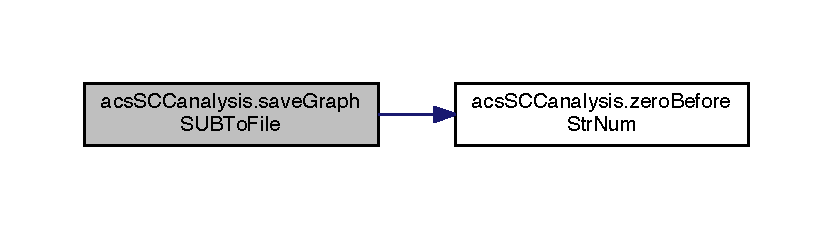
\includegraphics[width=350pt]{a00102_a5c959ea7dd3d2bd42004f1e5fd41f249_cgraph}
\end{center}
\end{figure}


\hypertarget{a00102_abf8df0ca8eb1c3ae9aeb0b20813d93d2}{\index{acs\-S\-C\-Canalysis@{acs\-S\-C\-Canalysis}!save\-Graph\-To\-File@{save\-Graph\-To\-File}}
\index{save\-Graph\-To\-File@{save\-Graph\-To\-File}!acsSCCanalysis@{acs\-S\-C\-Canalysis}}
\subsubsection[{save\-Graph\-To\-File}]{\setlength{\rightskip}{0pt plus 5cm}def acs\-S\-C\-Canalysis.\-save\-Graph\-To\-File (
\begin{DoxyParamCaption}
{}
\end{DoxyParamCaption}
)}}\label{a00102_abf8df0ca8eb1c3ae9aeb0b20813d93d2}


Definition at line 122 of file acs\-S\-C\-Canalysis.\-py.



Here is the call graph for this function\-:
\nopagebreak
\begin{figure}[H]
\begin{center}
\leavevmode
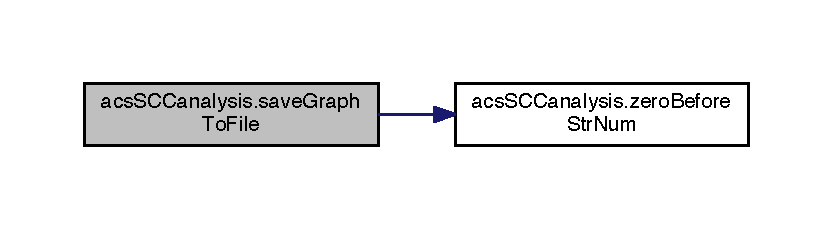
\includegraphics[width=350pt]{a00102_abf8df0ca8eb1c3ae9aeb0b20813d93d2_cgraph}
\end{center}
\end{figure}


\hypertarget{a00102_a541e9f38936fdf58fde0869521fdc5fc}{\index{acs\-S\-C\-Canalysis@{acs\-S\-C\-Canalysis}!save\-Nrg\-To\-File@{save\-Nrg\-To\-File}}
\index{save\-Nrg\-To\-File@{save\-Nrg\-To\-File}!acsSCCanalysis@{acs\-S\-C\-Canalysis}}
\subsubsection[{save\-Nrg\-To\-File}]{\setlength{\rightskip}{0pt plus 5cm}def acs\-S\-C\-Canalysis.\-save\-Nrg\-To\-File (
\begin{DoxyParamCaption}
{}
\end{DoxyParamCaption}
)}}\label{a00102_a541e9f38936fdf58fde0869521fdc5fc}


Definition at line 144 of file acs\-S\-C\-Canalysis.\-py.

\hypertarget{a00102_ab46df2a2027edcf1b07fc012b691b9d6}{\index{acs\-S\-C\-Canalysis@{acs\-S\-C\-Canalysis}!zero\-Before\-Str\-Num@{zero\-Before\-Str\-Num}}
\index{zero\-Before\-Str\-Num@{zero\-Before\-Str\-Num}!acsSCCanalysis@{acs\-S\-C\-Canalysis}}
\subsubsection[{zero\-Before\-Str\-Num}]{\setlength{\rightskip}{0pt plus 5cm}def acs\-S\-C\-Canalysis.\-zero\-Before\-Str\-Num (
\begin{DoxyParamCaption}
\item[{}]{tmpl, }
\item[{}]{tmp\-L}
\end{DoxyParamCaption}
)}}\label{a00102_ab46df2a2027edcf1b07fc012b691b9d6}


Definition at line 22 of file acs\-S\-C\-Canalysis.\-py.



Here is the caller graph for this function\-:
\nopagebreak
\begin{figure}[H]
\begin{center}
\leavevmode
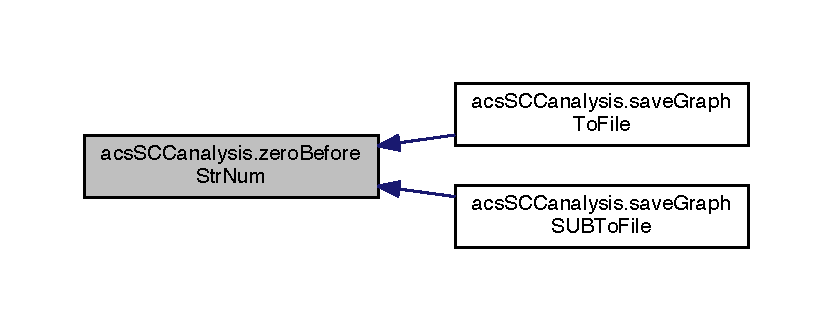
\includegraphics[width=350pt]{a00102_ab46df2a2027edcf1b07fc012b691b9d6_icgraph}
\end{center}
\end{figure}




\subsection{Variable Documentation}
\hypertarget{a00102_a46f1fb71bdcdb1c8679ae847d0d4b63f}{\index{acs\-S\-C\-Canalysis@{acs\-S\-C\-Canalysis}!\-\_\-\-A\-N\-A\-L\-T\-I\-M\-E\-I\-N\-T\-E\-R\-A\-V\-A\-L\-\_\-@{\-\_\-\-A\-N\-A\-L\-T\-I\-M\-E\-I\-N\-T\-E\-R\-A\-V\-A\-L\-\_\-}}
\index{\-\_\-\-A\-N\-A\-L\-T\-I\-M\-E\-I\-N\-T\-E\-R\-A\-V\-A\-L\-\_\-@{\-\_\-\-A\-N\-A\-L\-T\-I\-M\-E\-I\-N\-T\-E\-R\-A\-V\-A\-L\-\_\-}!acsSCCanalysis@{acs\-S\-C\-Canalysis}}
\subsubsection[{\-\_\-\-A\-N\-A\-L\-T\-I\-M\-E\-I\-N\-T\-E\-R\-A\-V\-A\-L\-\_\-}]{\setlength{\rightskip}{0pt plus 5cm}int acs\-S\-C\-Canalysis.\-\_\-\-A\-N\-A\-L\-T\-I\-M\-E\-I\-N\-T\-E\-R\-A\-V\-A\-L\-\_\- = {\bf tot\-Times}/10}}\label{a00102_a46f1fb71bdcdb1c8679ae847d0d4b63f}


Definition at line 269 of file acs\-S\-C\-Canalysis.\-py.

\hypertarget{a00102_a7665e828ed7f27f4ba353e9645ad716d}{\index{acs\-S\-C\-Canalysis@{acs\-S\-C\-Canalysis}!\-\_\-\-A\-N\-A\-L\-T\-I\-M\-E\-I\-N\-T\-E\-R\-A\-V\-A\-L\-N\-O\-S\-A\-V\-E\-\_\-@{\-\_\-\-A\-N\-A\-L\-T\-I\-M\-E\-I\-N\-T\-E\-R\-A\-V\-A\-L\-N\-O\-S\-A\-V\-E\-\_\-}}
\index{\-\_\-\-A\-N\-A\-L\-T\-I\-M\-E\-I\-N\-T\-E\-R\-A\-V\-A\-L\-N\-O\-S\-A\-V\-E\-\_\-@{\-\_\-\-A\-N\-A\-L\-T\-I\-M\-E\-I\-N\-T\-E\-R\-A\-V\-A\-L\-N\-O\-S\-A\-V\-E\-\_\-}!acsSCCanalysis@{acs\-S\-C\-Canalysis}}
\subsubsection[{\-\_\-\-A\-N\-A\-L\-T\-I\-M\-E\-I\-N\-T\-E\-R\-A\-V\-A\-L\-N\-O\-S\-A\-V\-E\-\_\-}]{\setlength{\rightskip}{0pt plus 5cm}int acs\-S\-C\-Canalysis.\-\_\-\-A\-N\-A\-L\-T\-I\-M\-E\-I\-N\-T\-E\-R\-A\-V\-A\-L\-N\-O\-S\-A\-V\-E\-\_\- = {\bf tot\-Times}/100}}\label{a00102_a7665e828ed7f27f4ba353e9645ad716d}


Definition at line 270 of file acs\-S\-C\-Canalysis.\-py.

\hypertarget{a00102_a98baad82b74a27e8b8c58aa985b7d374}{\index{acs\-S\-C\-Canalysis@{acs\-S\-C\-Canalysis}!age@{age}}
\index{age@{age}!acsSCCanalysis@{acs\-S\-C\-Canalysis}}
\subsubsection[{age}]{\setlength{\rightskip}{0pt plus 5cm}tuple acs\-S\-C\-Canalysis.\-age = float(tmp\-Age)}}\label{a00102_a98baad82b74a27e8b8c58aa985b7d374}


Definition at line 329 of file acs\-S\-C\-Canalysis.\-py.

\hypertarget{a00102_a38f20e6b1cad6a61f1c9b87b37c76f63}{\index{acs\-S\-C\-Canalysis@{acs\-S\-C\-Canalysis}!already\-Added\-\_\-\-A\-C\-S@{already\-Added\-\_\-\-A\-C\-S}}
\index{already\-Added\-\_\-\-A\-C\-S@{already\-Added\-\_\-\-A\-C\-S}!acsSCCanalysis@{acs\-S\-C\-Canalysis}}
\subsubsection[{already\-Added\-\_\-\-A\-C\-S}]{\setlength{\rightskip}{0pt plus 5cm}int acs\-S\-C\-Canalysis.\-already\-Added\-\_\-\-A\-C\-S = 0}}\label{a00102_a38f20e6b1cad6a61f1c9b87b37c76f63}


Definition at line 600 of file acs\-S\-C\-Canalysis.\-py.

\hypertarget{a00102_ac1b286545469555eb284f9b5f2bd984f}{\index{acs\-S\-C\-Canalysis@{acs\-S\-C\-Canalysis}!already\-Added\-\_\-chain@{already\-Added\-\_\-chain}}
\index{already\-Added\-\_\-chain@{already\-Added\-\_\-chain}!acsSCCanalysis@{acs\-S\-C\-Canalysis}}
\subsubsection[{already\-Added\-\_\-chain}]{\setlength{\rightskip}{0pt plus 5cm}int acs\-S\-C\-Canalysis.\-already\-Added\-\_\-chain = 0}}\label{a00102_ac1b286545469555eb284f9b5f2bd984f}


Definition at line 602 of file acs\-S\-C\-Canalysis.\-py.

\hypertarget{a00102_ac842390795cf193351c795945cde8e77}{\index{acs\-S\-C\-Canalysis@{acs\-S\-C\-Canalysis}!already\-Added\-\_\-leaves@{already\-Added\-\_\-leaves}}
\index{already\-Added\-\_\-leaves@{already\-Added\-\_\-leaves}!acsSCCanalysis@{acs\-S\-C\-Canalysis}}
\subsubsection[{already\-Added\-\_\-leaves}]{\setlength{\rightskip}{0pt plus 5cm}int acs\-S\-C\-Canalysis.\-already\-Added\-\_\-leaves = 0}}\label{a00102_ac842390795cf193351c795945cde8e77}


Definition at line 601 of file acs\-S\-C\-Canalysis.\-py.

\hypertarget{a00102_a70ccd5d519e878c6c8a7d0aa73caf46c}{\index{acs\-S\-C\-Canalysis@{acs\-S\-C\-Canalysis}!autocatalysis@{autocatalysis}}
\index{autocatalysis@{autocatalysis}!acsSCCanalysis@{acs\-S\-C\-Canalysis}}
\subsubsection[{autocatalysis}]{\setlength{\rightskip}{0pt plus 5cm}int acs\-S\-C\-Canalysis.\-autocatalysis = 0}}\label{a00102_a70ccd5d519e878c6c8a7d0aa73caf46c}


Definition at line 573 of file acs\-S\-C\-Canalysis.\-py.

\hypertarget{a00102_aea872e34fe0da6302f6195f1b2315148}{\index{acs\-S\-C\-Canalysis@{acs\-S\-C\-Canalysis}!cat@{cat}}
\index{cat@{cat}!acsSCCanalysis@{acs\-S\-C\-Canalysis}}
\subsubsection[{cat}]{\setlength{\rightskip}{0pt plus 5cm}tuple acs\-S\-C\-Canalysis.\-cat = int(tmp\-Cat)}}\label{a00102_aea872e34fe0da6302f6195f1b2315148}


Definition at line 411 of file acs\-S\-C\-Canalysis.\-py.

\hypertarget{a00102_a67fcb77a15f51e94c98bb48b05865715}{\index{acs\-S\-C\-Canalysis@{acs\-S\-C\-Canalysis}!cc@{cc}}
\index{cc@{cc}!acsSCCanalysis@{acs\-S\-C\-Canalysis}}
\subsubsection[{cc}]{\setlength{\rightskip}{0pt plus 5cm}tuple acs\-S\-C\-Canalysis.\-cc = int(tmpcc)}}\label{a00102_a67fcb77a15f51e94c98bb48b05865715}


Definition at line 410 of file acs\-S\-C\-Canalysis.\-py.

\hypertarget{a00102_a0dd6730b063ac11ae4620c4a0778f6d9}{\index{acs\-S\-C\-Canalysis@{acs\-S\-C\-Canalysis}!cleavage\-\_\-counter@{cleavage\-\_\-counter}}
\index{cleavage\-\_\-counter@{cleavage\-\_\-counter}!acsSCCanalysis@{acs\-S\-C\-Canalysis}}
\subsubsection[{cleavage\-\_\-counter}]{\setlength{\rightskip}{0pt plus 5cm}int acs\-S\-C\-Canalysis.\-cleavage\-\_\-counter = 0}}\label{a00102_a0dd6730b063ac11ae4620c4a0778f6d9}


Definition at line 392 of file acs\-S\-C\-Canalysis.\-py.

\hypertarget{a00102_a0a501feb02e67bd6a8ba75490709cf89}{\index{acs\-S\-C\-Canalysis@{acs\-S\-C\-Canalysis}!cmd\-File\-Fid@{cmd\-File\-Fid}}
\index{cmd\-File\-Fid@{cmd\-File\-Fid}!acsSCCanalysis@{acs\-S\-C\-Canalysis}}
\subsubsection[{cmd\-File\-Fid}]{\setlength{\rightskip}{0pt plus 5cm}tuple acs\-S\-C\-Canalysis.\-cmd\-File\-Fid = open({\bf cmd\-File\-Name}, '{\bf a}')}}\label{a00102_a0a501feb02e67bd6a8ba75490709cf89}


Definition at line 185 of file acs\-S\-C\-Canalysis.\-py.

\hypertarget{a00102_a32551f85ad3cd8080b8ad81828276368}{\index{acs\-S\-C\-Canalysis@{acs\-S\-C\-Canalysis}!cmd\-File\-Name@{cmd\-File\-Name}}
\index{cmd\-File\-Name@{cmd\-File\-Name}!acsSCCanalysis@{acs\-S\-C\-Canalysis}}
\subsubsection[{cmd\-File\-Name}]{\setlength{\rightskip}{0pt plus 5cm}string acs\-S\-C\-Canalysis.\-cmd\-File\-Name = {\bf Str\-Path}+'/'}}\label{a00102_a32551f85ad3cd8080b8ad81828276368}


Definition at line 182 of file acs\-S\-C\-Canalysis.\-py.

\hypertarget{a00102_a6ec435b19c74f79f32a0eae7bb2bd1c8}{\index{acs\-S\-C\-Canalysis@{acs\-S\-C\-Canalysis}!conc@{conc}}
\index{conc@{conc}!acsSCCanalysis@{acs\-S\-C\-Canalysis}}
\subsubsection[{conc}]{\setlength{\rightskip}{0pt plus 5cm}tuple acs\-S\-C\-Canalysis.\-conc = float(tmp\-Conc)}}\label{a00102_a6ec435b19c74f79f32a0eae7bb2bd1c8}


Definition at line 327 of file acs\-S\-C\-Canalysis.\-py.

\hypertarget{a00102_aac2f508d526d62bd7f9d4f5a5f8b1821}{\index{acs\-S\-C\-Canalysis@{acs\-S\-C\-Canalysis}!conc\-\_\-by\-S\-C\-C@{conc\-\_\-by\-S\-C\-C}}
\index{conc\-\_\-by\-S\-C\-C@{conc\-\_\-by\-S\-C\-C}!acsSCCanalysis@{acs\-S\-C\-Canalysis}}
\subsubsection[{conc\-\_\-by\-S\-C\-C}]{\setlength{\rightskip}{0pt plus 5cm}int acs\-S\-C\-Canalysis.\-conc\-\_\-by\-S\-C\-C = 0}}\label{a00102_aac2f508d526d62bd7f9d4f5a5f8b1821}


Definition at line 581 of file acs\-S\-C\-Canalysis.\-py.

\hypertarget{a00102_a3188cc39362e42ecb36d23a98f2b5a78}{\index{acs\-S\-C\-Canalysis@{acs\-S\-C\-Canalysis}!conc\-\_\-chain@{conc\-\_\-chain}}
\index{conc\-\_\-chain@{conc\-\_\-chain}!acsSCCanalysis@{acs\-S\-C\-Canalysis}}
\subsubsection[{conc\-\_\-chain}]{\setlength{\rightskip}{0pt plus 5cm}int acs\-S\-C\-Canalysis.\-conc\-\_\-chain = 0}}\label{a00102_a3188cc39362e42ecb36d23a98f2b5a78}


Definition at line 580 of file acs\-S\-C\-Canalysis.\-py.

\hypertarget{a00102_a3fcb8f9c7e88b5c53f1201a383b38666}{\index{acs\-S\-C\-Canalysis@{acs\-S\-C\-Canalysis}!conc\-\_\-in\-S\-C\-C@{conc\-\_\-in\-S\-C\-C}}
\index{conc\-\_\-in\-S\-C\-C@{conc\-\_\-in\-S\-C\-C}!acsSCCanalysis@{acs\-S\-C\-Canalysis}}
\subsubsection[{conc\-\_\-in\-S\-C\-C}]{\setlength{\rightskip}{0pt plus 5cm}int acs\-S\-C\-Canalysis.\-conc\-\_\-in\-S\-C\-C = 0}}\label{a00102_a3fcb8f9c7e88b5c53f1201a383b38666}


Definition at line 579 of file acs\-S\-C\-Canalysis.\-py.

\hypertarget{a00102_afd3169174539244248b78c8da2bba265}{\index{acs\-S\-C\-Canalysis@{acs\-S\-C\-Canalysis}!conc\-\_\-over\-Lap@{conc\-\_\-over\-Lap}}
\index{conc\-\_\-over\-Lap@{conc\-\_\-over\-Lap}!acsSCCanalysis@{acs\-S\-C\-Canalysis}}
\subsubsection[{conc\-\_\-over\-Lap}]{\setlength{\rightskip}{0pt plus 5cm}int acs\-S\-C\-Canalysis.\-conc\-\_\-over\-Lap = 0}}\label{a00102_afd3169174539244248b78c8da2bba265}


Definition at line 582 of file acs\-S\-C\-Canalysis.\-py.

\hypertarget{a00102_a9e8cc07f7d7f892f3f72274318dcbcef}{\index{acs\-S\-C\-Canalysis@{acs\-S\-C\-Canalysis}!conc\-\_\-self\-Cat@{conc\-\_\-self\-Cat}}
\index{conc\-\_\-self\-Cat@{conc\-\_\-self\-Cat}!acsSCCanalysis@{acs\-S\-C\-Canalysis}}
\subsubsection[{conc\-\_\-self\-Cat}]{\setlength{\rightskip}{0pt plus 5cm}int acs\-S\-C\-Canalysis.\-conc\-\_\-self\-Cat = 0}}\label{a00102_a9e8cc07f7d7f892f3f72274318dcbcef}


Definition at line 583 of file acs\-S\-C\-Canalysis.\-py.

\hypertarget{a00102_a1681853ab5f5859e51f219caa07a8539}{\index{acs\-S\-C\-Canalysis@{acs\-S\-C\-Canalysis}!conc\-Vec@{conc\-Vec}}
\index{conc\-Vec@{conc\-Vec}!acsSCCanalysis@{acs\-S\-C\-Canalysis}}
\subsubsection[{conc\-Vec}]{\setlength{\rightskip}{0pt plus 5cm}list acs\-S\-C\-Canalysis.\-conc\-Vec = \mbox{[}$\,$\mbox{]}}}\label{a00102_a1681853ab5f5859e51f219caa07a8539}


Definition at line 318 of file acs\-S\-C\-Canalysis.\-py.

\hypertarget{a00102_a144441bdbe6e835849cf165ea2946848}{\index{acs\-S\-C\-Canalysis@{acs\-S\-C\-Canalysis}!condensation\-\_\-counter@{condensation\-\_\-counter}}
\index{condensation\-\_\-counter@{condensation\-\_\-counter}!acsSCCanalysis@{acs\-S\-C\-Canalysis}}
\subsubsection[{condensation\-\_\-counter}]{\setlength{\rightskip}{0pt plus 5cm}int acs\-S\-C\-Canalysis.\-condensation\-\_\-counter = 0}}\label{a00102_a144441bdbe6e835849cf165ea2946848}


Definition at line 390 of file acs\-S\-C\-Canalysis.\-py.

\hypertarget{a00102_a06673ec4592e44a89a443073b8a29011}{\index{acs\-S\-C\-Canalysis@{acs\-S\-C\-Canalysis}!cpx\-Cut@{cpx\-Cut}}
\index{cpx\-Cut@{cpx\-Cut}!acsSCCanalysis@{acs\-S\-C\-Canalysis}}
\subsubsection[{cpx\-Cut}]{\setlength{\rightskip}{0pt plus 5cm}tuple acs\-S\-C\-Canalysis.\-cpx\-Cut = int(tmp\-Cpx\-Cut)}}\label{a00102_a06673ec4592e44a89a443073b8a29011}


Definition at line 328 of file acs\-S\-C\-Canalysis.\-py.

\hypertarget{a00102_a80a6d3cf3f4ccdc596054300761972a9}{\index{acs\-S\-C\-Canalysis@{acs\-S\-C\-Canalysis}!decay\-Time@{decay\-Time}}
\index{decay\-Time@{decay\-Time}!acsSCCanalysis@{acs\-S\-C\-Canalysis}}
\subsubsection[{decay\-Time}]{\setlength{\rightskip}{0pt plus 5cm}tuple acs\-S\-C\-Canalysis.\-decay\-Time = int({\bf str\-Line}\mbox{[}1\mbox{]})}}\label{a00102_a80a6d3cf3f4ccdc596054300761972a9}


Definition at line 255 of file acs\-S\-C\-Canalysis.\-py.

\hypertarget{a00102_af5702a39b502da88dde8c38417a0efbd}{\index{acs\-S\-C\-Canalysis@{acs\-S\-C\-Canalysis}!endo\-\_\-cleavage\-\_\-counter@{endo\-\_\-cleavage\-\_\-counter}}
\index{endo\-\_\-cleavage\-\_\-counter@{endo\-\_\-cleavage\-\_\-counter}!acsSCCanalysis@{acs\-S\-C\-Canalysis}}
\subsubsection[{endo\-\_\-cleavage\-\_\-counter}]{\setlength{\rightskip}{0pt plus 5cm}int acs\-S\-C\-Canalysis.\-endo\-\_\-cleavage\-\_\-counter = 0}}\label{a00102_af5702a39b502da88dde8c38417a0efbd}


Definition at line 391 of file acs\-S\-C\-Canalysis.\-py.

\hypertarget{a00102_a20a51ec68106a5a97fb3a72f417ca4e6}{\index{acs\-S\-C\-Canalysis@{acs\-S\-C\-Canalysis}!endo\-\_\-condensation\-\_\-counter@{endo\-\_\-condensation\-\_\-counter}}
\index{endo\-\_\-condensation\-\_\-counter@{endo\-\_\-condensation\-\_\-counter}!acsSCCanalysis@{acs\-S\-C\-Canalysis}}
\subsubsection[{endo\-\_\-condensation\-\_\-counter}]{\setlength{\rightskip}{0pt plus 5cm}int acs\-S\-C\-Canalysis.\-endo\-\_\-condensation\-\_\-counter = 0}}\label{a00102_a20a51ec68106a5a97fb3a72f417ca4e6}


Definition at line 389 of file acs\-S\-C\-Canalysis.\-py.

\hypertarget{a00102_a424e2204e89264a827e6cad861ebcbc1}{\index{acs\-S\-C\-Canalysis@{acs\-S\-C\-Canalysis}!fid@{fid}}
\index{fid@{fid}!acsSCCanalysis@{acs\-S\-C\-Canalysis}}
\subsubsection[{fid}]{\setlength{\rightskip}{0pt plus 5cm}tuple acs\-S\-C\-Canalysis.\-fid = open({\bf param\-File}, '{\bf r}')}}\label{a00102_a424e2204e89264a827e6cad861ebcbc1}


Definition at line 244 of file acs\-S\-C\-Canalysis.\-py.

\hypertarget{a00102_a0c40e4d9928e8df792b31c7a431d3fba}{\index{acs\-S\-C\-Canalysis@{acs\-S\-C\-Canalysis}!fidflux@{fidflux}}
\index{fidflux@{fidflux}!acsSCCanalysis@{acs\-S\-C\-Canalysis}}
\subsubsection[{fidflux}]{\setlength{\rightskip}{0pt plus 5cm}tuple acs\-S\-C\-Canalysis.\-fidflux = open('\-\_\-acsinflux.\-csv', '{\bf r}')}}\label{a00102_a0c40e4d9928e8df792b31c7a431d3fba}


Definition at line 285 of file acs\-S\-C\-Canalysis.\-py.

\hypertarget{a00102_aba2f982879776e057b35971b3653549e}{\index{acs\-S\-C\-Canalysis@{acs\-S\-C\-Canalysis}!fid\-Species@{fid\-Species}}
\index{fid\-Species@{fid\-Species}!acsSCCanalysis@{acs\-S\-C\-Canalysis}}
\subsubsection[{fid\-Species}]{\setlength{\rightskip}{0pt plus 5cm}tuple acs\-S\-C\-Canalysis.\-fid\-Species = open({\bf species\-File}, '{\bf r}')}}\label{a00102_aba2f982879776e057b35971b3653549e}


Definition at line 311 of file acs\-S\-C\-Canalysis.\-py.

\hypertarget{a00102_a60ff937c050eef601bd84134d1913d8a}{\index{acs\-S\-C\-Canalysis@{acs\-S\-C\-Canalysis}!filext\-Pre@{filext\-Pre}}
\index{filext\-Pre@{filext\-Pre}!acsSCCanalysis@{acs\-S\-C\-Canalysis}}
\subsubsection[{filext\-Pre}]{\setlength{\rightskip}{0pt plus 5cm}string acs\-S\-C\-Canalysis.\-filext\-Pre = '\-\_\-'}}\label{a00102_a60ff937c050eef601bd84134d1913d8a}


Definition at line 376 of file acs\-S\-C\-Canalysis.\-py.

\hypertarget{a00102_a1cbfd083273176eebfe0260e8384acef}{\index{acs\-S\-C\-Canalysis@{acs\-S\-C\-Canalysis}!folder\-Cat@{folder\-Cat}}
\index{folder\-Cat@{folder\-Cat}!acsSCCanalysis@{acs\-S\-C\-Canalysis}}
\subsubsection[{folder\-Cat}]{\setlength{\rightskip}{0pt plus 5cm}string acs\-S\-C\-Canalysis.\-folder\-Cat = '\-\_\-\-\_\-0\-\_\-i\-Graph\-\_\-\-C\-A\-T\-\_\-'}}\label{a00102_a1cbfd083273176eebfe0260e8384acef}


Definition at line 348 of file acs\-S\-C\-Canalysis.\-py.

\hypertarget{a00102_a90c2bcabbdb271c2c3347ebea4c259bc}{\index{acs\-S\-C\-Canalysis@{acs\-S\-C\-Canalysis}!folder\-Sub@{folder\-Sub}}
\index{folder\-Sub@{folder\-Sub}!acsSCCanalysis@{acs\-S\-C\-Canalysis}}
\subsubsection[{folder\-Sub}]{\setlength{\rightskip}{0pt plus 5cm}string acs\-S\-C\-Canalysis.\-folder\-Sub = '\-\_\-\-\_\-0\-\_\-i\-Graph\-\_\-\-S\-U\-B\-\_\-'}}\label{a00102_a90c2bcabbdb271c2c3347ebea4c259bc}


Definition at line 349 of file acs\-S\-C\-Canalysis.\-py.

\hypertarget{a00102_ad88c3dd8eb89ddbe8720462b03f35003}{\index{acs\-S\-C\-Canalysis@{acs\-S\-C\-Canalysis}!Gcatpro@{Gcatpro}}
\index{Gcatpro@{Gcatpro}!acsSCCanalysis@{acs\-S\-C\-Canalysis}}
\subsubsection[{Gcatpro}]{\setlength{\rightskip}{0pt plus 5cm}tuple acs\-S\-C\-Canalysis.\-Gcatpro = nx.\-Di\-Graph()}}\label{a00102_ad88c3dd8eb89ddbe8720462b03f35003}


Definition at line 555 of file acs\-S\-C\-Canalysis.\-py.

\hypertarget{a00102_a4c214eb4f6812d6182bae32715bce3ad}{\index{acs\-S\-C\-Canalysis@{acs\-S\-C\-Canalysis}!gill\-Entropy@{gill\-Entropy}}
\index{gill\-Entropy@{gill\-Entropy}!acsSCCanalysis@{acs\-S\-C\-Canalysis}}
\subsubsection[{gill\-Entropy}]{\setlength{\rightskip}{0pt plus 5cm}tuple acs\-S\-C\-Canalysis.\-gill\-Entropy = float(tmp\-Gill\-Entropy)}}\label{a00102_a4c214eb4f6812d6182bae32715bce3ad}


Definition at line 419 of file acs\-S\-C\-Canalysis.\-py.

\hypertarget{a00102_a4e862896701636d17752f14810ff687f}{\index{acs\-S\-C\-Canalysis@{acs\-S\-C\-Canalysis}!gill\-Mean@{gill\-Mean}}
\index{gill\-Mean@{gill\-Mean}!acsSCCanalysis@{acs\-S\-C\-Canalysis}}
\subsubsection[{gill\-Mean}]{\setlength{\rightskip}{0pt plus 5cm}tuple acs\-S\-C\-Canalysis.\-gill\-Mean = float(tmp\-Gill\-Mean)}}\label{a00102_a4e862896701636d17752f14810ff687f}


Definition at line 417 of file acs\-S\-C\-Canalysis.\-py.

\hypertarget{a00102_acdb3e72aea08c29494799fd08763b406}{\index{acs\-S\-C\-Canalysis@{acs\-S\-C\-Canalysis}!gill\-S\-D@{gill\-S\-D}}
\index{gill\-S\-D@{gill\-S\-D}!acsSCCanalysis@{acs\-S\-C\-Canalysis}}
\subsubsection[{gill\-S\-D}]{\setlength{\rightskip}{0pt plus 5cm}tuple acs\-S\-C\-Canalysis.\-gill\-S\-D = float(tmp\-Gill\-S\-D)}}\label{a00102_acdb3e72aea08c29494799fd08763b406}


Definition at line 418 of file acs\-S\-C\-Canalysis.\-py.

\hypertarget{a00102_a99669fe823cebc560b46c3746f9183e7}{\index{acs\-S\-C\-Canalysis@{acs\-S\-C\-Canalysis}!gill\-Time\-Series@{gill\-Time\-Series}}
\index{gill\-Time\-Series@{gill\-Time\-Series}!acsSCCanalysis@{acs\-S\-C\-Canalysis}}
\subsubsection[{gill\-Time\-Series}]{\setlength{\rightskip}{0pt plus 5cm}tuple acs\-S\-C\-Canalysis.\-gill\-Time\-Series = np.\-array(\mbox{[}\mbox{[}0,0,0,0\mbox{]}\mbox{]})}}\label{a00102_a99669fe823cebc560b46c3746f9183e7}


Definition at line 399 of file acs\-S\-C\-Canalysis.\-py.

\hypertarget{a00102_ab45392da38059bf7557c22cbc73e5580}{\index{acs\-S\-C\-Canalysis@{acs\-S\-C\-Canalysis}!graph@{graph}}
\index{graph@{graph}!acsSCCanalysis@{acs\-S\-C\-Canalysis}}
\subsubsection[{graph}]{\setlength{\rightskip}{0pt plus 5cm}tuple acs\-S\-C\-Canalysis.\-graph = {\bf load\-Specific\-Reaction\-Graph}()}}\label{a00102_ab45392da38059bf7557c22cbc73e5580}


Definition at line 193 of file acs\-S\-C\-Canalysis.\-py.

\hypertarget{a00102_ae307841da4a073fad4f6eaa172b0b970}{\index{acs\-S\-C\-Canalysis@{acs\-S\-C\-Canalysis}!graph\-S\-U\-B@{graph\-S\-U\-B}}
\index{graph\-S\-U\-B@{graph\-S\-U\-B}!acsSCCanalysis@{acs\-S\-C\-Canalysis}}
\subsubsection[{graph\-S\-U\-B}]{\setlength{\rightskip}{0pt plus 5cm}tuple acs\-S\-C\-Canalysis.\-graph\-S\-U\-B = {\bf load\-Specific\-Reaction\-Sub\-Graph}()}}\label{a00102_ae307841da4a073fad4f6eaa172b0b970}


Definition at line 194 of file acs\-S\-C\-Canalysis.\-py.

\hypertarget{a00102_a578f0f0f1e87579d73b11f8720610b1e}{\index{acs\-S\-C\-Canalysis@{acs\-S\-C\-Canalysis}!I\-Ds\-Over\-Threshold@{I\-Ds\-Over\-Threshold}}
\index{I\-Ds\-Over\-Threshold@{I\-Ds\-Over\-Threshold}!acsSCCanalysis@{acs\-S\-C\-Canalysis}}
\subsubsection[{I\-Ds\-Over\-Threshold}]{\setlength{\rightskip}{0pt plus 5cm}list acs\-S\-C\-Canalysis.\-I\-Ds\-Over\-Threshold = \mbox{[}$\,$\mbox{]}}}\label{a00102_a578f0f0f1e87579d73b11f8720610b1e}


Definition at line 317 of file acs\-S\-C\-Canalysis.\-py.

\hypertarget{a00102_a540ba5319ee67d8a2323099dad73ba36}{\index{acs\-S\-C\-Canalysis@{acs\-S\-C\-Canalysis}!incoming\-Nodes@{incoming\-Nodes}}
\index{incoming\-Nodes@{incoming\-Nodes}!acsSCCanalysis@{acs\-S\-C\-Canalysis}}
\subsubsection[{incoming\-Nodes}]{\setlength{\rightskip}{0pt plus 5cm}tuple acs\-S\-C\-Canalysis.\-incoming\-Nodes = Gcatpro.\-predecessors(Ids\-O\-T)}}\label{a00102_a540ba5319ee67d8a2323099dad73ba36}


Definition at line 605 of file acs\-S\-C\-Canalysis.\-py.

\hypertarget{a00102_a5004d18b8cfa2803620a9cd7f32d9775}{\index{acs\-S\-C\-Canalysis@{acs\-S\-C\-Canalysis}!in\-Degree\-Mean@{in\-Degree\-Mean}}
\index{in\-Degree\-Mean@{in\-Degree\-Mean}!acsSCCanalysis@{acs\-S\-C\-Canalysis}}
\subsubsection[{in\-Degree\-Mean}]{\setlength{\rightskip}{0pt plus 5cm}tuple acs\-S\-C\-Canalysis.\-in\-Degree\-Mean = mean(Gcatpro.\-in\-\_\-degree().values())}}\label{a00102_a5004d18b8cfa2803620a9cd7f32d9775}


Definition at line 682 of file acs\-S\-C\-Canalysis.\-py.

\hypertarget{a00102_aaac3bb67a998c4a09aeed8f1adec2f9c}{\index{acs\-S\-C\-Canalysis@{acs\-S\-C\-Canalysis}!index@{index}}
\index{index@{index}!acsSCCanalysis@{acs\-S\-C\-Canalysis}}
\subsubsection[{index}]{\setlength{\rightskip}{0pt plus 5cm}tuple acs\-S\-C\-Canalysis.\-index = int(tmp\-I\-D)}}\label{a00102_aaac3bb67a998c4a09aeed8f1adec2f9c}


Definition at line 326 of file acs\-S\-C\-Canalysis.\-py.

\hypertarget{a00102_a3a8adee26325d72aca909e91b0fd3ea5}{\index{acs\-S\-C\-Canalysis@{acs\-S\-C\-Canalysis}!influx\-\_\-rate@{influx\-\_\-rate}}
\index{influx\-\_\-rate@{influx\-\_\-rate}!acsSCCanalysis@{acs\-S\-C\-Canalysis}}
\subsubsection[{influx\-\_\-rate}]{\setlength{\rightskip}{0pt plus 5cm}tuple acs\-S\-C\-Canalysis.\-influx\-\_\-rate = float({\bf str\-Line}\mbox{[}1\mbox{]})}}\label{a00102_a3a8adee26325d72aca909e91b0fd3ea5}


Definition at line 264 of file acs\-S\-C\-Canalysis.\-py.

\hypertarget{a00102_ac6ad18bfc83e8ea3254897d46f990855}{\index{acs\-S\-C\-Canalysis@{acs\-S\-C\-Canalysis}!initilize\-Graph\-Structure@{initilize\-Graph\-Structure}}
\index{initilize\-Graph\-Structure@{initilize\-Graph\-Structure}!acsSCCanalysis@{acs\-S\-C\-Canalysis}}
\subsubsection[{initilize\-Graph\-Structure}]{\setlength{\rightskip}{0pt plus 5cm}int acs\-S\-C\-Canalysis.\-initilize\-Graph\-Structure = 0}}\label{a00102_ac6ad18bfc83e8ea3254897d46f990855}


Definition at line 189 of file acs\-S\-C\-Canalysis.\-py.

\hypertarget{a00102_a212643643fc6b002e8797f16633bb16d}{\index{acs\-S\-C\-Canalysis@{acs\-S\-C\-Canalysis}!init\-Rct\-Id@{init\-Rct\-Id}}
\index{init\-Rct\-Id@{init\-Rct\-Id}!acsSCCanalysis@{acs\-S\-C\-Canalysis}}
\subsubsection[{init\-Rct\-Id}]{\setlength{\rightskip}{0pt plus 5cm}int acs\-S\-C\-Canalysis.\-init\-Rct\-Id = int({\bf tmp\-Rct\-File\-To\-Load\-Split\-String}\mbox{[}len({\bf tmp\-Rct\-File\-To\-Load\-Split\-String})-\/2\mbox{]})}}\label{a00102_a212643643fc6b002e8797f16633bb16d}


Definition at line 198 of file acs\-S\-C\-Canalysis.\-py.

\hypertarget{a00102_adc4403c4cfe080918c8b9da692c50509}{\index{acs\-S\-C\-Canalysis@{acs\-S\-C\-Canalysis}!init\-Temp\-Time@{init\-Temp\-Time}}
\index{init\-Temp\-Time@{init\-Temp\-Time}!acsSCCanalysis@{acs\-S\-C\-Canalysis}}
\subsubsection[{init\-Temp\-Time}]{\setlength{\rightskip}{0pt plus 5cm}list acs\-S\-C\-Canalysis.\-init\-Temp\-Time = {\bf tmp\-Rct\-File\-To\-Load\-Split\-String}\mbox{[}len({\bf tmp\-Rct\-File\-To\-Load\-Split\-String})-\/1\mbox{]}}}\label{a00102_adc4403c4cfe080918c8b9da692c50509}


Definition at line 199 of file acs\-S\-C\-Canalysis.\-py.

\hypertarget{a00102_a826c1b0585b4e8474c76f92bd7583836}{\index{acs\-S\-C\-Canalysis@{acs\-S\-C\-Canalysis}!init\-Time@{init\-Time}}
\index{init\-Time@{init\-Time}!acsSCCanalysis@{acs\-S\-C\-Canalysis}}
\subsubsection[{init\-Time}]{\setlength{\rightskip}{0pt plus 5cm}int acs\-S\-C\-Canalysis.\-init\-Time = float({\bf init\-Temp\-Time}\mbox{[}0\-:len({\bf init\-Temp\-Time})-\/4\mbox{]})}}\label{a00102_a826c1b0585b4e8474c76f92bd7583836}


Definition at line 200 of file acs\-S\-C\-Canalysis.\-py.

\hypertarget{a00102_a6405b6b05e7b87812422cc30d2034904}{\index{acs\-S\-C\-Canalysis@{acs\-S\-C\-Canalysis}!in\-S\-C\-C\-Flag@{in\-S\-C\-C\-Flag}}
\index{in\-S\-C\-C\-Flag@{in\-S\-C\-C\-Flag}!acsSCCanalysis@{acs\-S\-C\-Canalysis}}
\subsubsection[{in\-S\-C\-C\-Flag}]{\setlength{\rightskip}{0pt plus 5cm}int acs\-S\-C\-Canalysis.\-in\-S\-C\-C\-Flag = 0}}\label{a00102_a6405b6b05e7b87812422cc30d2034904}


Definition at line 616 of file acs\-S\-C\-Canalysis.\-py.

\hypertarget{a00102_ab4566d46d368eb4f93ff6db5191648bd}{\index{acs\-S\-C\-Canalysis@{acs\-S\-C\-Canalysis}!loaded\-Mols@{loaded\-Mols}}
\index{loaded\-Mols@{loaded\-Mols}!acsSCCanalysis@{acs\-S\-C\-Canalysis}}
\subsubsection[{loaded\-Mols}]{\setlength{\rightskip}{0pt plus 5cm}tuple acs\-S\-C\-Canalysis.\-loaded\-Mols = int(tmp\-Loaded\-Mols)}}\label{a00102_ab4566d46d368eb4f93ff6db5191648bd}


Definition at line 416 of file acs\-S\-C\-Canalysis.\-py.

\hypertarget{a00102_abe83f5e0ae3bd65da15a697a979aeea1}{\index{acs\-S\-C\-Canalysis@{acs\-S\-C\-Canalysis}!loaded\-Mols\-Conc@{loaded\-Mols\-Conc}}
\index{loaded\-Mols\-Conc@{loaded\-Mols\-Conc}!acsSCCanalysis@{acs\-S\-C\-Canalysis}}
\subsubsection[{loaded\-Mols\-Conc}]{\setlength{\rightskip}{0pt plus 5cm}tuple acs\-S\-C\-Canalysis.\-loaded\-Mols\-Conc = float(tmp\-Loaded\-Mols\-Conc)}}\label{a00102_abe83f5e0ae3bd65da15a697a979aeea1}


Definition at line 415 of file acs\-S\-C\-Canalysis.\-py.

\hypertarget{a00102_a47da7b9153a0e4a33512f6d2675b8c1a}{\index{acs\-S\-C\-Canalysis@{acs\-S\-C\-Canalysis}!max\-L\-Out@{max\-L\-Out}}
\index{max\-L\-Out@{max\-L\-Out}!acsSCCanalysis@{acs\-S\-C\-Canalysis}}
\subsubsection[{max\-L\-Out}]{\setlength{\rightskip}{0pt plus 5cm}tuple acs\-S\-C\-Canalysis.\-max\-L\-Out = float({\bf str\-Line}\mbox{[}1\mbox{]})}}\label{a00102_a47da7b9153a0e4a33512f6d2675b8c1a}


Definition at line 266 of file acs\-S\-C\-Canalysis.\-py.

\hypertarget{a00102_af10c3623be709892f4bdc4df5a3d52b0}{\index{acs\-S\-C\-Canalysis@{acs\-S\-C\-Canalysis}!mean\-Over\-Threshold@{mean\-Over\-Threshold}}
\index{mean\-Over\-Threshold@{mean\-Over\-Threshold}!acsSCCanalysis@{acs\-S\-C\-Canalysis}}
\subsubsection[{mean\-Over\-Threshold}]{\setlength{\rightskip}{0pt plus 5cm}tuple acs\-S\-C\-Canalysis.\-mean\-Over\-Threshold = float({\bf over\-Threshold})}}\label{a00102_af10c3623be709892f4bdc4df5a3d52b0}


Definition at line 703 of file acs\-S\-C\-Canalysis.\-py.

\hypertarget{a00102_ae13d6607ffa236891a9af05bfa88cfcc}{\index{acs\-S\-C\-Canalysis@{acs\-S\-C\-Canalysis}!mol\-\_\-\-I@{mol\-\_\-\-I}}
\index{mol\-\_\-\-I@{mol\-\_\-\-I}!acsSCCanalysis@{acs\-S\-C\-Canalysis}}
\subsubsection[{mol\-\_\-\-I}]{\setlength{\rightskip}{0pt plus 5cm}tuple acs\-S\-C\-Canalysis.\-mol\-\_\-\-I = int(tmp\-Mol\-\_\-\-I)}}\label{a00102_ae13d6607ffa236891a9af05bfa88cfcc}


Definition at line 412 of file acs\-S\-C\-Canalysis.\-py.

\hypertarget{a00102_a8f2878f5909e4aeb9155a1103eaba413}{\index{acs\-S\-C\-Canalysis@{acs\-S\-C\-Canalysis}!mol\-\_\-\-I\-I@{mol\-\_\-\-I\-I}}
\index{mol\-\_\-\-I\-I@{mol\-\_\-\-I\-I}!acsSCCanalysis@{acs\-S\-C\-Canalysis}}
\subsubsection[{mol\-\_\-\-I\-I}]{\setlength{\rightskip}{0pt plus 5cm}tuple acs\-S\-C\-Canalysis.\-mol\-\_\-\-I\-I = int(tmp\-Mol\-\_\-\-I\-I)}}\label{a00102_a8f2878f5909e4aeb9155a1103eaba413}


Definition at line 413 of file acs\-S\-C\-Canalysis.\-py.

\hypertarget{a00102_a20047e8516f386a7e98ffa0efec09471}{\index{acs\-S\-C\-Canalysis@{acs\-S\-C\-Canalysis}!mol\-\_\-\-I\-I\-I@{mol\-\_\-\-I\-I\-I}}
\index{mol\-\_\-\-I\-I\-I@{mol\-\_\-\-I\-I\-I}!acsSCCanalysis@{acs\-S\-C\-Canalysis}}
\subsubsection[{mol\-\_\-\-I\-I\-I}]{\setlength{\rightskip}{0pt plus 5cm}tuple acs\-S\-C\-Canalysis.\-mol\-\_\-\-I\-I\-I = int(tmp\-Mol\-\_\-\-I\-I\-I)}}\label{a00102_a20047e8516f386a7e98ffa0efec09471}


Definition at line 414 of file acs\-S\-C\-Canalysis.\-py.

\hypertarget{a00102_a2abf09620dd1dd990036c67c626b3dee}{\index{acs\-S\-C\-Canalysis@{acs\-S\-C\-Canalysis}!mswindows@{mswindows}}
\index{mswindows@{mswindows}!acsSCCanalysis@{acs\-S\-C\-Canalysis}}
\subsubsection[{mswindows}]{\setlength{\rightskip}{0pt plus 5cm}tuple acs\-S\-C\-Canalysis.\-mswindows = (sys.\-platform == \char`\"{}win32\char`\"{})}}\label{a00102_a2abf09620dd1dd990036c67c626b3dee}


Definition at line 179 of file acs\-S\-C\-Canalysis.\-py.

\hypertarget{a00102_a440179ca1c764cabcf9181985ae5dfb8}{\index{acs\-S\-C\-Canalysis@{acs\-S\-C\-Canalysis}!newdir@{newdir}}
\index{newdir@{newdir}!acsSCCanalysis@{acs\-S\-C\-Canalysis}}
\subsubsection[{newdir}]{\setlength{\rightskip}{0pt plus 5cm}tuple acs\-S\-C\-Canalysis.\-newdir = os.\-path.\-join(os.\-curdir, {\bf folder\-Cat})}}\label{a00102_a440179ca1c764cabcf9181985ae5dfb8}


Definition at line 356 of file acs\-S\-C\-Canalysis.\-py.

\hypertarget{a00102_adb3b62d0896774bc87adfee19d047aa8}{\index{acs\-S\-C\-Canalysis@{acs\-S\-C\-Canalysis}!newdir\-S\-U\-B@{newdir\-S\-U\-B}}
\index{newdir\-S\-U\-B@{newdir\-S\-U\-B}!acsSCCanalysis@{acs\-S\-C\-Canalysis}}
\subsubsection[{newdir\-S\-U\-B}]{\setlength{\rightskip}{0pt plus 5cm}tuple acs\-S\-C\-Canalysis.\-newdir\-S\-U\-B = os.\-path.\-join(os.\-curdir, {\bf folder\-Sub})}}\label{a00102_adb3b62d0896774bc87adfee19d047aa8}


Definition at line 365 of file acs\-S\-C\-Canalysis.\-py.

\hypertarget{a00102_a47b24df6e487f6dd90158dde93cc7c93}{\index{acs\-S\-C\-Canalysis@{acs\-S\-C\-Canalysis}!new\-Species\-Creation\-Prob@{new\-Species\-Creation\-Prob}}
\index{new\-Species\-Creation\-Prob@{new\-Species\-Creation\-Prob}!acsSCCanalysis@{acs\-S\-C\-Canalysis}}
\subsubsection[{new\-Species\-Creation\-Prob}]{\setlength{\rightskip}{0pt plus 5cm}tuple acs\-S\-C\-Canalysis.\-new\-Species\-Creation\-Prob = float(tmp\-N\-S\-Cprob)}}\label{a00102_a47b24df6e487f6dd90158dde93cc7c93}


Definition at line 420 of file acs\-S\-C\-Canalysis.\-py.

\hypertarget{a00102_a4766b3ca835449f1aa287fda699c7f96}{\index{acs\-S\-C\-Canalysis@{acs\-S\-C\-Canalysis}!no\-In\-Acs@{no\-In\-Acs}}
\index{no\-In\-Acs@{no\-In\-Acs}!acsSCCanalysis@{acs\-S\-C\-Canalysis}}
\subsubsection[{no\-In\-Acs}]{\setlength{\rightskip}{0pt plus 5cm}int acs\-S\-C\-Canalysis.\-no\-In\-Acs = 1}}\label{a00102_a4766b3ca835449f1aa287fda699c7f96}


Definition at line 612 of file acs\-S\-C\-Canalysis.\-py.

\hypertarget{a00102_a948683f966c62ac856582281c3cda1f4}{\index{acs\-S\-C\-Canalysis@{acs\-S\-C\-Canalysis}!nrg@{nrg}}
\index{nrg@{nrg}!acsSCCanalysis@{acs\-S\-C\-Canalysis}}
\subsubsection[{nrg}]{\setlength{\rightskip}{0pt plus 5cm}int acs\-S\-C\-Canalysis.\-nrg = 1}}\label{a00102_a948683f966c62ac856582281c3cda1f4}


Definition at line 273 of file acs\-S\-C\-Canalysis.\-py.

\hypertarget{a00102_a24d5f5a61d56c596017396ad272ef4a4}{\index{acs\-S\-C\-Canalysis@{acs\-S\-C\-Canalysis}!nrg\-Conc@{nrg\-Conc}}
\index{nrg\-Conc@{nrg\-Conc}!acsSCCanalysis@{acs\-S\-C\-Canalysis}}
\subsubsection[{nrg\-Conc}]{\setlength{\rightskip}{0pt plus 5cm}tuple acs\-S\-C\-Canalysis.\-nrg\-Conc = float({\bf str\-Line}\mbox{[}1\mbox{]})}}\label{a00102_a24d5f5a61d56c596017396ad272ef4a4}


Definition at line 262 of file acs\-S\-C\-Canalysis.\-py.

\hypertarget{a00102_ad4d4abc783f2f7f8d1084b1144b4fe2f}{\index{acs\-S\-C\-Canalysis@{acs\-S\-C\-Canalysis}!nrg\-Time\-Series@{nrg\-Time\-Series}}
\index{nrg\-Time\-Series@{nrg\-Time\-Series}!acsSCCanalysis@{acs\-S\-C\-Canalysis}}
\subsubsection[{nrg\-Time\-Series}]{\setlength{\rightskip}{0pt plus 5cm}tuple acs\-S\-C\-Canalysis.\-nrg\-Time\-Series = np.\-array(\mbox{[}\mbox{[}0,0,0\mbox{]}\mbox{]})}}\label{a00102_ad4d4abc783f2f7f8d1084b1144b4fe2f}


Definition at line 397 of file acs\-S\-C\-Canalysis.\-py.

\hypertarget{a00102_a0d0c83fd90489be59b1f5a31dadf4469}{\index{acs\-S\-C\-Canalysis@{acs\-S\-C\-Canalysis}!nrg\-Type@{nrg\-Type}}
\index{nrg\-Type@{nrg\-Type}!acsSCCanalysis@{acs\-S\-C\-Canalysis}}
\subsubsection[{nrg\-Type}]{\setlength{\rightskip}{0pt plus 5cm}tuple acs\-S\-C\-Canalysis.\-nrg\-Type = int({\bf str\-Line}\mbox{[}1\mbox{]})}}\label{a00102_a0d0c83fd90489be59b1f5a31dadf4469}


Definition at line 258 of file acs\-S\-C\-Canalysis.\-py.

\hypertarget{a00102_a9a81829f850e2e125e3c94214da7a1f0}{\index{acs\-S\-C\-Canalysis@{acs\-S\-C\-Canalysis}!number\-Of\-Gen@{number\-Of\-Gen}}
\index{number\-Of\-Gen@{number\-Of\-Gen}!acsSCCanalysis@{acs\-S\-C\-Canalysis}}
\subsubsection[{number\-Of\-Gen}]{\setlength{\rightskip}{0pt plus 5cm}tuple acs\-S\-C\-Canalysis.\-number\-Of\-Gen = len(glob.\-glob(os.\-path.\-join({\bf res\-Dir\-Path},'times\-\_\-$\ast$')))}}\label{a00102_a9a81829f850e2e125e3c94214da7a1f0}


Definition at line 230 of file acs\-S\-C\-Canalysis.\-py.

\hypertarget{a00102_a9ce833d782f17d858941cfa76914599a}{\index{acs\-S\-C\-Canalysis@{acs\-S\-C\-Canalysis}!ok@{ok}}
\index{ok@{ok}!acsSCCanalysis@{acs\-S\-C\-Canalysis}}
\subsubsection[{ok}]{\setlength{\rightskip}{0pt plus 5cm}int acs\-S\-C\-Canalysis.\-ok = 0}}\label{a00102_a9ce833d782f17d858941cfa76914599a}


Definition at line 316 of file acs\-S\-C\-Canalysis.\-py.

\hypertarget{a00102_a12e61f8d7aadb52256a7728af342bae3}{\index{acs\-S\-C\-Canalysis@{acs\-S\-C\-Canalysis}!over\-Threshold@{over\-Threshold}}
\index{over\-Threshold@{over\-Threshold}!acsSCCanalysis@{acs\-S\-C\-Canalysis}}
\subsubsection[{over\-Threshold}]{\setlength{\rightskip}{0pt plus 5cm}tuple acs\-S\-C\-Canalysis.\-over\-Threshold = float(0)}}\label{a00102_a12e61f8d7aadb52256a7728af342bae3}


Definition at line 299 of file acs\-S\-C\-Canalysis.\-py.

\hypertarget{a00102_a93de20dd9ebf791127ac5aefc0a2df8d}{\index{acs\-S\-C\-Canalysis@{acs\-S\-C\-Canalysis}!over\-Threshold\-T\-O\-T@{over\-Threshold\-T\-O\-T}}
\index{over\-Threshold\-T\-O\-T@{over\-Threshold\-T\-O\-T}!acsSCCanalysis@{acs\-S\-C\-Canalysis}}
\subsubsection[{over\-Threshold\-T\-O\-T}]{\setlength{\rightskip}{0pt plus 5cm}tuple acs\-S\-C\-Canalysis.\-over\-Threshold\-T\-O\-T = float(0)}}\label{a00102_a93de20dd9ebf791127ac5aefc0a2df8d}


Definition at line 300 of file acs\-S\-C\-Canalysis.\-py.

\hypertarget{a00102_a7160f8e48b4aafebbd75e9037fc9fef7}{\index{acs\-S\-C\-Canalysis@{acs\-S\-C\-Canalysis}!param\-File@{param\-File}}
\index{param\-File@{param\-File}!acsSCCanalysis@{acs\-S\-C\-Canalysis}}
\subsubsection[{param\-File}]{\setlength{\rightskip}{0pt plus 5cm}string acs\-S\-C\-Canalysis.\-param\-File = \char`\"{}acsm2s.\-conf\char`\"{}}}\label{a00102_a7160f8e48b4aafebbd75e9037fc9fef7}


Definition at line 241 of file acs\-S\-C\-Canalysis.\-py.

\hypertarget{a00102_ac09e85f8df5b7c8c7d2caf87e9193421}{\index{acs\-S\-C\-Canalysis@{acs\-S\-C\-Canalysis}!position@{position}}
\index{position@{position}!acsSCCanalysis@{acs\-S\-C\-Canalysis}}
\subsubsection[{position}]{\setlength{\rightskip}{0pt plus 5cm}tuple acs\-S\-C\-Canalysis.\-position = (({\bf graph}\mbox{[}\-:,0\mbox{]} == {\bf cat}) \& ({\bf graph}\mbox{[}\-:,1\mbox{]} == {\bf mol\-\_\-\-I}))}}\label{a00102_ac09e85f8df5b7c8c7d2caf87e9193421}


Definition at line 482 of file acs\-S\-C\-Canalysis.\-py.

\hypertarget{a00102_aff96a31e98ac46cb47a67b74f5d87351}{\index{acs\-S\-C\-Canalysis@{acs\-S\-C\-Canalysis}!previous\-Time@{previous\-Time}}
\index{previous\-Time@{previous\-Time}!acsSCCanalysis@{acs\-S\-C\-Canalysis}}
\subsubsection[{previous\-Time}]{\setlength{\rightskip}{0pt plus 5cm}acs\-S\-C\-Canalysis.\-previous\-Time = 0}}\label{a00102_aff96a31e98ac46cb47a67b74f5d87351}


Definition at line 386 of file acs\-S\-C\-Canalysis.\-py.

\hypertarget{a00102_a3de1ee32e24403b152d565d8c52cf7fd}{\index{acs\-S\-C\-Canalysis@{acs\-S\-C\-Canalysis}!print\-Temporal\-Message@{print\-Temporal\-Message}}
\index{print\-Temporal\-Message@{print\-Temporal\-Message}!acsSCCanalysis@{acs\-S\-C\-Canalysis}}
\subsubsection[{print\-Temporal\-Message}]{\setlength{\rightskip}{0pt plus 5cm}int acs\-S\-C\-Canalysis.\-print\-Temporal\-Message = 1}}\label{a00102_a3de1ee32e24403b152d565d8c52cf7fd}


Definition at line 428 of file acs\-S\-C\-Canalysis.\-py.

\hypertarget{a00102_abb2ac92624837ae48b882d145c5aab11}{\index{acs\-S\-C\-Canalysis@{acs\-S\-C\-Canalysis}!prod\-\_\-by\-S\-C\-C@{prod\-\_\-by\-S\-C\-C}}
\index{prod\-\_\-by\-S\-C\-C@{prod\-\_\-by\-S\-C\-C}!acsSCCanalysis@{acs\-S\-C\-Canalysis}}
\subsubsection[{prod\-\_\-by\-S\-C\-C}]{\setlength{\rightskip}{0pt plus 5cm}int acs\-S\-C\-Canalysis.\-prod\-\_\-by\-S\-C\-C = 0}}\label{a00102_abb2ac92624837ae48b882d145c5aab11}


Definition at line 570 of file acs\-S\-C\-Canalysis.\-py.

\hypertarget{a00102_a5f45dbe461b3b18021c93780e87cc40e}{\index{acs\-S\-C\-Canalysis@{acs\-S\-C\-Canalysis}!prod\-\_\-by\-S\-C\-C\-\_\-weight@{prod\-\_\-by\-S\-C\-C\-\_\-weight}}
\index{prod\-\_\-by\-S\-C\-C\-\_\-weight@{prod\-\_\-by\-S\-C\-C\-\_\-weight}!acsSCCanalysis@{acs\-S\-C\-Canalysis}}
\subsubsection[{prod\-\_\-by\-S\-C\-C\-\_\-weight}]{\setlength{\rightskip}{0pt plus 5cm}int acs\-S\-C\-Canalysis.\-prod\-\_\-by\-S\-C\-C\-\_\-weight = 0}}\label{a00102_a5f45dbe461b3b18021c93780e87cc40e}


Definition at line 576 of file acs\-S\-C\-Canalysis.\-py.

\hypertarget{a00102_ab307c6047e4d16ec0335266b24e7db5a}{\index{acs\-S\-C\-Canalysis@{acs\-S\-C\-Canalysis}!prod\-\_\-chain@{prod\-\_\-chain}}
\index{prod\-\_\-chain@{prod\-\_\-chain}!acsSCCanalysis@{acs\-S\-C\-Canalysis}}
\subsubsection[{prod\-\_\-chain}]{\setlength{\rightskip}{0pt plus 5cm}int acs\-S\-C\-Canalysis.\-prod\-\_\-chain = 0}}\label{a00102_ab307c6047e4d16ec0335266b24e7db5a}


Definition at line 569 of file acs\-S\-C\-Canalysis.\-py.

\hypertarget{a00102_a6736365f1f19058f6e1d57287383dbcc}{\index{acs\-S\-C\-Canalysis@{acs\-S\-C\-Canalysis}!prod\-\_\-chain\-\_\-weight@{prod\-\_\-chain\-\_\-weight}}
\index{prod\-\_\-chain\-\_\-weight@{prod\-\_\-chain\-\_\-weight}!acsSCCanalysis@{acs\-S\-C\-Canalysis}}
\subsubsection[{prod\-\_\-chain\-\_\-weight}]{\setlength{\rightskip}{0pt plus 5cm}int acs\-S\-C\-Canalysis.\-prod\-\_\-chain\-\_\-weight = 0}}\label{a00102_a6736365f1f19058f6e1d57287383dbcc}


Definition at line 575 of file acs\-S\-C\-Canalysis.\-py.

\hypertarget{a00102_adbc76b0558ceb74d798b35146a583474}{\index{acs\-S\-C\-Canalysis@{acs\-S\-C\-Canalysis}!prod\-\_\-in\-S\-C\-C@{prod\-\_\-in\-S\-C\-C}}
\index{prod\-\_\-in\-S\-C\-C@{prod\-\_\-in\-S\-C\-C}!acsSCCanalysis@{acs\-S\-C\-Canalysis}}
\subsubsection[{prod\-\_\-in\-S\-C\-C}]{\setlength{\rightskip}{0pt plus 5cm}int acs\-S\-C\-Canalysis.\-prod\-\_\-in\-S\-C\-C = 0}}\label{a00102_adbc76b0558ceb74d798b35146a583474}


Definition at line 568 of file acs\-S\-C\-Canalysis.\-py.

\hypertarget{a00102_aa22adccedd9ae548d0687df507ebd92d}{\index{acs\-S\-C\-Canalysis@{acs\-S\-C\-Canalysis}!prod\-\_\-in\-S\-C\-C\-\_\-weight@{prod\-\_\-in\-S\-C\-C\-\_\-weight}}
\index{prod\-\_\-in\-S\-C\-C\-\_\-weight@{prod\-\_\-in\-S\-C\-C\-\_\-weight}!acsSCCanalysis@{acs\-S\-C\-Canalysis}}
\subsubsection[{prod\-\_\-in\-S\-C\-C\-\_\-weight}]{\setlength{\rightskip}{0pt plus 5cm}int acs\-S\-C\-Canalysis.\-prod\-\_\-in\-S\-C\-C\-\_\-weight = 0}}\label{a00102_aa22adccedd9ae548d0687df507ebd92d}


Definition at line 574 of file acs\-S\-C\-Canalysis.\-py.

\hypertarget{a00102_a213e964195f0666d00663ca874a09caa}{\index{acs\-S\-C\-Canalysis@{acs\-S\-C\-Canalysis}!prod\-\_\-overlap@{prod\-\_\-overlap}}
\index{prod\-\_\-overlap@{prod\-\_\-overlap}!acsSCCanalysis@{acs\-S\-C\-Canalysis}}
\subsubsection[{prod\-\_\-overlap}]{\setlength{\rightskip}{0pt plus 5cm}int acs\-S\-C\-Canalysis.\-prod\-\_\-overlap = 0}}\label{a00102_a213e964195f0666d00663ca874a09caa}


Definition at line 571 of file acs\-S\-C\-Canalysis.\-py.

\hypertarget{a00102_ab78b07d6cd1a94356c4fee43dfc1272a}{\index{acs\-S\-C\-Canalysis@{acs\-S\-C\-Canalysis}!prod\-\_\-overlap\-\_\-weight@{prod\-\_\-overlap\-\_\-weight}}
\index{prod\-\_\-overlap\-\_\-weight@{prod\-\_\-overlap\-\_\-weight}!acsSCCanalysis@{acs\-S\-C\-Canalysis}}
\subsubsection[{prod\-\_\-overlap\-\_\-weight}]{\setlength{\rightskip}{0pt plus 5cm}int acs\-S\-C\-Canalysis.\-prod\-\_\-overlap\-\_\-weight = 0}}\label{a00102_ab78b07d6cd1a94356c4fee43dfc1272a}


Definition at line 577 of file acs\-S\-C\-Canalysis.\-py.

\hypertarget{a00102_a78ffc7d3b69c53ec5389a151e7fdcb83}{\index{acs\-S\-C\-Canalysis@{acs\-S\-C\-Canalysis}!rct\-I\-D@{rct\-I\-D}}
\index{rct\-I\-D@{rct\-I\-D}!acsSCCanalysis@{acs\-S\-C\-Canalysis}}
\subsubsection[{rct\-I\-D}]{\setlength{\rightskip}{0pt plus 5cm}int acs\-S\-C\-Canalysis.\-rct\-I\-D = {\bf init\-Rct\-Id}}}\label{a00102_a78ffc7d3b69c53ec5389a151e7fdcb83}


Definition at line 385 of file acs\-S\-C\-Canalysis.\-py.

\hypertarget{a00102_a8a780c7762bc8a40f296abfd474b7ce4}{\index{acs\-S\-C\-Canalysis@{acs\-S\-C\-Canalysis}!rct\-I\-Dshow@{rct\-I\-Dshow}}
\index{rct\-I\-Dshow@{rct\-I\-Dshow}!acsSCCanalysis@{acs\-S\-C\-Canalysis}}
\subsubsection[{rct\-I\-Dshow}]{\setlength{\rightskip}{0pt plus 5cm}int acs\-S\-C\-Canalysis.\-rct\-I\-Dshow = 1.\-0}}\label{a00102_a8a780c7762bc8a40f296abfd474b7ce4}


Definition at line 383 of file acs\-S\-C\-Canalysis.\-py.

\hypertarget{a00102_a3942b0b71d5893c244f7f49929db336b}{\index{acs\-S\-C\-Canalysis@{acs\-S\-C\-Canalysis}!rct\-I\-Dshow\-No\-Save@{rct\-I\-Dshow\-No\-Save}}
\index{rct\-I\-Dshow\-No\-Save@{rct\-I\-Dshow\-No\-Save}!acsSCCanalysis@{acs\-S\-C\-Canalysis}}
\subsubsection[{rct\-I\-Dshow\-No\-Save}]{\setlength{\rightskip}{0pt plus 5cm}int acs\-S\-C\-Canalysis.\-rct\-I\-Dshow\-No\-Save = 1.\-0}}\label{a00102_a3942b0b71d5893c244f7f49929db336b}


Definition at line 384 of file acs\-S\-C\-Canalysis.\-py.

\hypertarget{a00102_ac700504fc38d7684ec9fae104d7d90a3}{\index{acs\-S\-C\-Canalysis@{acs\-S\-C\-Canalysis}!rct\-Param\-File@{rct\-Param\-File}}
\index{rct\-Param\-File@{rct\-Param\-File}!acsSCCanalysis@{acs\-S\-C\-Canalysis}}
\subsubsection[{rct\-Param\-File}]{\setlength{\rightskip}{0pt plus 5cm}tuple acs\-S\-C\-Canalysis.\-rct\-Param\-File = sorted(glob.\-glob(os.\-path.\-join({\bf res\-Dir\-Path},{\bf rct\-Param\-File\-Q})))}}\label{a00102_ac700504fc38d7684ec9fae104d7d90a3}


Definition at line 380 of file acs\-S\-C\-Canalysis.\-py.

\hypertarget{a00102_aff5ea475bb2c78122a231a915dc88e89}{\index{acs\-S\-C\-Canalysis@{acs\-S\-C\-Canalysis}!rct\-Param\-File\-Q@{rct\-Param\-File\-Q}}
\index{rct\-Param\-File\-Q@{rct\-Param\-File\-Q}!acsSCCanalysis@{acs\-S\-C\-Canalysis}}
\subsubsection[{rct\-Param\-File\-Q}]{\setlength{\rightskip}{0pt plus 5cm}string acs\-S\-C\-Canalysis.\-rct\-Param\-File\-Q = 'reactions\-\_\-parameters\-\_\-'}}\label{a00102_aff5ea475bb2c78122a231a915dc88e89}


Definition at line 379 of file acs\-S\-C\-Canalysis.\-py.

\hypertarget{a00102_a58c3618ec28f27dfbf09e0d3aba05bc7}{\index{acs\-S\-C\-Canalysis@{acs\-S\-C\-Canalysis}!reaction@{reaction}}
\index{reaction@{reaction}!acsSCCanalysis@{acs\-S\-C\-Canalysis}}
\subsubsection[{reaction}]{\setlength{\rightskip}{0pt plus 5cm}tuple acs\-S\-C\-Canalysis.\-reaction = int(tmp\-Reaction)}}\label{a00102_a58c3618ec28f27dfbf09e0d3aba05bc7}


Definition at line 408 of file acs\-S\-C\-Canalysis.\-py.

\hypertarget{a00102_ac6aaa0ac5d13b0736ab3179dc1ed388d}{\index{acs\-S\-C\-Canalysis@{acs\-S\-C\-Canalysis}!real\-Sccs@{real\-Sccs}}
\index{real\-Sccs@{real\-Sccs}!acsSCCanalysis@{acs\-S\-C\-Canalysis}}
\subsubsection[{real\-Sccs}]{\setlength{\rightskip}{0pt plus 5cm}int acs\-S\-C\-Canalysis.\-real\-Sccs = 0}}\label{a00102_ac6aaa0ac5d13b0736ab3179dc1ed388d}


Definition at line 554 of file acs\-S\-C\-Canalysis.\-py.

\hypertarget{a00102_a1c9b45f6074222ace96b7ab38cb8e23b}{\index{acs\-S\-C\-Canalysis@{acs\-S\-C\-Canalysis}!real\-T@{real\-T}}
\index{real\-T@{real\-T}!acsSCCanalysis@{acs\-S\-C\-Canalysis}}
\subsubsection[{real\-T}]{\setlength{\rightskip}{0pt plus 5cm}acs\-S\-C\-Canalysis.\-real\-T = {\bf threshold}}}\label{a00102_a1c9b45f6074222ace96b7ab38cb8e23b}


Definition at line 333 of file acs\-S\-C\-Canalysis.\-py.

\hypertarget{a00102_a9ededb3cd7c63befde39ad68e5f9e006}{\index{acs\-S\-C\-Canalysis@{acs\-S\-C\-Canalysis}!res\-Dir\-Path@{res\-Dir\-Path}}
\index{res\-Dir\-Path@{res\-Dir\-Path}!acsSCCanalysis@{acs\-S\-C\-Canalysis}}
\subsubsection[{res\-Dir\-Path}]{\setlength{\rightskip}{0pt plus 5cm}tuple acs\-S\-C\-Canalysis.\-res\-Dir\-Path = os.\-path.\-abspath(os.\-path.\-join(\char`\"{}./\char`\"{}, \char`\"{}res\char`\"{}))}}\label{a00102_a9ededb3cd7c63befde39ad68e5f9e006}


Definition at line 223 of file acs\-S\-C\-Canalysis.\-py.

\hypertarget{a00102_aa7db2dba66810044f9c5238eccc995b7}{\index{acs\-S\-C\-Canalysis@{acs\-S\-C\-Canalysis}!reverse\-Probability@{reverse\-Probability}}
\index{reverse\-Probability@{reverse\-Probability}!acsSCCanalysis@{acs\-S\-C\-Canalysis}}
\subsubsection[{reverse\-Probability}]{\setlength{\rightskip}{0pt plus 5cm}tuple acs\-S\-C\-Canalysis.\-reverse\-Probability = float(tmp\-Rev\-Prob)}}\label{a00102_aa7db2dba66810044f9c5238eccc995b7}


Definition at line 421 of file acs\-S\-C\-Canalysis.\-py.

\hypertarget{a00102_a98150f532e09ebae495212500d2f1799}{\index{acs\-S\-C\-Canalysis@{acs\-S\-C\-Canalysis}!rp@{rp}}
\index{rp@{rp}!acsSCCanalysis@{acs\-S\-C\-Canalysis}}
\subsubsection[{rp}]{\setlength{\rightskip}{0pt plus 5cm}tuple acs\-S\-C\-Canalysis.\-rp = float({\bf str\-Line}\mbox{[}1\mbox{]})}}\label{a00102_a98150f532e09ebae495212500d2f1799}


Definition at line 252 of file acs\-S\-C\-Canalysis.\-py.

\hypertarget{a00102_a162a08b0497058c76e7e885c03a01336}{\index{acs\-S\-C\-Canalysis@{acs\-S\-C\-Canalysis}!rtime@{rtime}}
\index{rtime@{rtime}!acsSCCanalysis@{acs\-S\-C\-Canalysis}}
\subsubsection[{rtime}]{\setlength{\rightskip}{0pt plus 5cm}tuple acs\-S\-C\-Canalysis.\-rtime = float(tmp\-Time)}}\label{a00102_a162a08b0497058c76e7e885c03a01336}


Definition at line 409 of file acs\-S\-C\-Canalysis.\-py.

\hypertarget{a00102_a2094b7f0917a16a948a2d1c4d700e84c}{\index{acs\-S\-C\-Canalysis@{acs\-S\-C\-Canalysis}!scc@{scc}}
\index{scc@{scc}!acsSCCanalysis@{acs\-S\-C\-Canalysis}}
\subsubsection[{scc}]{\setlength{\rightskip}{0pt plus 5cm}tuple acs\-S\-C\-Canalysis.\-scc = nx.\-strongly\-\_\-connected\-\_\-components({\bf Gcatpro})}}\label{a00102_a2094b7f0917a16a948a2d1c4d700e84c}


Definition at line 561 of file acs\-S\-C\-Canalysis.\-py.

\hypertarget{a00102_a1dd3c43841ba4485a66889600f099a0c}{\index{acs\-S\-C\-Canalysis@{acs\-S\-C\-Canalysis}!scc\-I\-D@{scc\-I\-D}}
\index{scc\-I\-D@{scc\-I\-D}!acsSCCanalysis@{acs\-S\-C\-Canalysis}}
\subsubsection[{scc\-I\-D}]{\setlength{\rightskip}{0pt plus 5cm}int acs\-S\-C\-Canalysis.\-scc\-I\-D = 0}}\label{a00102_a1dd3c43841ba4485a66889600f099a0c}


Definition at line 572 of file acs\-S\-C\-Canalysis.\-py.

\hypertarget{a00102_a185cbf8ef1ec67f52695562582418793}{\index{acs\-S\-C\-Canalysis@{acs\-S\-C\-Canalysis}!scc\-N@{scc\-N}}
\index{scc\-N@{scc\-N}!acsSCCanalysis@{acs\-S\-C\-Canalysis}}
\subsubsection[{scc\-N}]{\setlength{\rightskip}{0pt plus 5cm}tuple acs\-S\-C\-Canalysis.\-scc\-N = nx.\-number\-\_\-strongly\-\_\-connected\-\_\-components({\bf Gcatpro})}}\label{a00102_a185cbf8ef1ec67f52695562582418793}


Definition at line 562 of file acs\-S\-C\-Canalysis.\-py.

\hypertarget{a00102_ae9790fbc87f233c94224436a9cbd59c1}{\index{acs\-S\-C\-Canalysis@{acs\-S\-C\-Canalysis}!self\-\_\-loop\-\_\-weight@{self\-\_\-loop\-\_\-weight}}
\index{self\-\_\-loop\-\_\-weight@{self\-\_\-loop\-\_\-weight}!acsSCCanalysis@{acs\-S\-C\-Canalysis}}
\subsubsection[{self\-\_\-loop\-\_\-weight}]{\setlength{\rightskip}{0pt plus 5cm}int acs\-S\-C\-Canalysis.\-self\-\_\-loop\-\_\-weight = 0}}\label{a00102_ae9790fbc87f233c94224436a9cbd59c1}


Definition at line 578 of file acs\-S\-C\-Canalysis.\-py.

\hypertarget{a00102_a8fec45ae9b70981ce94eaeed14d888b1}{\index{acs\-S\-C\-Canalysis@{acs\-S\-C\-Canalysis}!self\-Loops@{self\-Loops}}
\index{self\-Loops@{self\-Loops}!acsSCCanalysis@{acs\-S\-C\-Canalysis}}
\subsubsection[{self\-Loops}]{\setlength{\rightskip}{0pt plus 5cm}tuple acs\-S\-C\-Canalysis.\-self\-Loops = Gcatpro.\-number\-\_\-of\-\_\-selfloops()}}\label{a00102_a8fec45ae9b70981ce94eaeed14d888b1}


Definition at line 563 of file acs\-S\-C\-Canalysis.\-py.

\hypertarget{a00102_ad34596e89eef2cfb696f61a810765c7a}{\index{acs\-S\-C\-Canalysis@{acs\-S\-C\-Canalysis}!self\-Loops\-Egdes@{self\-Loops\-Egdes}}
\index{self\-Loops\-Egdes@{self\-Loops\-Egdes}!acsSCCanalysis@{acs\-S\-C\-Canalysis}}
\subsubsection[{self\-Loops\-Egdes}]{\setlength{\rightskip}{0pt plus 5cm}tuple acs\-S\-C\-Canalysis.\-self\-Loops\-Egdes = Gcatpro.\-selfloop\-\_\-edges()}}\label{a00102_ad34596e89eef2cfb696f61a810765c7a}


Definition at line 564 of file acs\-S\-C\-Canalysis.\-py.

\hypertarget{a00102_a58095f64afeda893517e81226e1963c3}{\index{acs\-S\-C\-Canalysis@{acs\-S\-C\-Canalysis}!sim\-Folder@{sim\-Folder}}
\index{sim\-Folder@{sim\-Folder}!acsSCCanalysis@{acs\-S\-C\-Canalysis}}
\subsubsection[{sim\-Folder}]{\setlength{\rightskip}{0pt plus 5cm}int acs\-S\-C\-Canalysis.\-sim\-Folder = 0}}\label{a00102_a58095f64afeda893517e81226e1963c3}


Definition at line 242 of file acs\-S\-C\-Canalysis.\-py.

\hypertarget{a00102_a1d066fa24dced2da12ffd9a8514a17ba}{\index{acs\-S\-C\-Canalysis@{acs\-S\-C\-Canalysis}!species\-File@{species\-File}}
\index{species\-File@{species\-File}!acsSCCanalysis@{acs\-S\-C\-Canalysis}}
\subsubsection[{species\-File}]{\setlength{\rightskip}{0pt plus 5cm}list acs\-S\-C\-Canalysis.\-species\-File = {\bf species\-Files}\mbox{[}-\/1\mbox{]}}}\label{a00102_a1d066fa24dced2da12ffd9a8514a17ba}


Definition at line 305 of file acs\-S\-C\-Canalysis.\-py.

\hypertarget{a00102_a4f47408478e9a0590d016df50cf42141}{\index{acs\-S\-C\-Canalysis@{acs\-S\-C\-Canalysis}!species\-Files@{species\-Files}}
\index{species\-Files@{species\-Files}!acsSCCanalysis@{acs\-S\-C\-Canalysis}}
\subsubsection[{species\-Files}]{\setlength{\rightskip}{0pt plus 5cm}tuple acs\-S\-C\-Canalysis.\-species\-Files = sorted(glob.\-glob(os.\-path.\-join({\bf res\-Dir\-Path},{\bf tmp\-Files\-To\-Search})))}}\label{a00102_a4f47408478e9a0590d016df50cf42141}


Definition at line 304 of file acs\-S\-C\-Canalysis.\-py.

\hypertarget{a00102_a36f6b63269e716f42cd38a36a781a4cf}{\index{acs\-S\-C\-Canalysis@{acs\-S\-C\-Canalysis}!species\-In\-Flux@{species\-In\-Flux}}
\index{species\-In\-Flux@{species\-In\-Flux}!acsSCCanalysis@{acs\-S\-C\-Canalysis}}
\subsubsection[{species\-In\-Flux}]{\setlength{\rightskip}{0pt plus 5cm}list acs\-S\-C\-Canalysis.\-species\-In\-Flux = range(0,int(pow(2,({\bf max\-L\-Out}+1)) -\/ 2))}}\label{a00102_a36f6b63269e716f42cd38a36a781a4cf}


Definition at line 280 of file acs\-S\-C\-Canalysis.\-py.

\hypertarget{a00102_a072631e11db72789389935b0f9efff8d}{\index{acs\-S\-C\-Canalysis@{acs\-S\-C\-Canalysis}!str\-Line@{str\-Line}}
\index{str\-Line@{str\-Line}!acsSCCanalysis@{acs\-S\-C\-Canalysis}}
\subsubsection[{str\-Line}]{\setlength{\rightskip}{0pt plus 5cm}tuple acs\-S\-C\-Canalysis.\-str\-Line = {\bf line.\-split}('=')}}\label{a00102_a072631e11db72789389935b0f9efff8d}


Definition at line 250 of file acs\-S\-C\-Canalysis.\-py.

\hypertarget{a00102_af8add8b37a9c8a7825c0e8f0e7dfd6c1}{\index{acs\-S\-C\-Canalysis@{acs\-S\-C\-Canalysis}!Str\-Path@{Str\-Path}}
\index{Str\-Path@{Str\-Path}!acsSCCanalysis@{acs\-S\-C\-Canalysis}}
\subsubsection[{Str\-Path}]{\setlength{\rightskip}{0pt plus 5cm}tuple acs\-S\-C\-Canalysis.\-Str\-Path = os.\-path.\-abspath(Str\-Path)}}\label{a00102_af8add8b37a9c8a7825c0e8f0e7dfd6c1}


Definition at line 177 of file acs\-S\-C\-Canalysis.\-py.

\hypertarget{a00102_a1966f0657c6b477eeb60bde732a201cc}{\index{acs\-S\-C\-Canalysis@{acs\-S\-C\-Canalysis}!str\-To\-Write@{str\-To\-Write}}
\index{str\-To\-Write@{str\-To\-Write}!acsSCCanalysis@{acs\-S\-C\-Canalysis}}
\subsubsection[{str\-To\-Write}]{\setlength{\rightskip}{0pt plus 5cm}string acs\-S\-C\-Canalysis.\-str\-To\-Write = \char`\"{}\textbackslash{}t\-Reaction Probability\char`\"{}}}\label{a00102_a1966f0657c6b477eeb60bde732a201cc}


Definition at line 186 of file acs\-S\-C\-Canalysis.\-py.

\hypertarget{a00102_a8ba6aefb71b3d1e575eac38627f143d6}{\index{acs\-S\-C\-Canalysis@{acs\-S\-C\-Canalysis}!str\-Zeros@{str\-Zeros}}
\index{str\-Zeros@{str\-Zeros}!acsSCCanalysis@{acs\-S\-C\-Canalysis}}
\subsubsection[{str\-Zeros}]{\setlength{\rightskip}{0pt plus 5cm}tuple acs\-S\-C\-Canalysis.\-str\-Zeros = {\bf zero\-Before\-Str\-Num}(n\-Gen, {\bf number\-Of\-Gen})}}\label{a00102_a8ba6aefb71b3d1e575eac38627f143d6}


Definition at line 238 of file acs\-S\-C\-Canalysis.\-py.

\hypertarget{a00102_aaf17c99825e0961e4cfaa173ddfffe84}{\index{acs\-S\-C\-Canalysis@{acs\-S\-C\-Canalysis}!temp\-Prod\-\_\-chain\-\_\-weight@{temp\-Prod\-\_\-chain\-\_\-weight}}
\index{temp\-Prod\-\_\-chain\-\_\-weight@{temp\-Prod\-\_\-chain\-\_\-weight}!acsSCCanalysis@{acs\-S\-C\-Canalysis}}
\subsubsection[{temp\-Prod\-\_\-chain\-\_\-weight}]{\setlength{\rightskip}{0pt plus 5cm}int acs\-S\-C\-Canalysis.\-temp\-Prod\-\_\-chain\-\_\-weight = 0}}\label{a00102_aaf17c99825e0961e4cfaa173ddfffe84}


Definition at line 607 of file acs\-S\-C\-Canalysis.\-py.

\hypertarget{a00102_a7d0f86310c439e970e0b41121364027c}{\index{acs\-S\-C\-Canalysis@{acs\-S\-C\-Canalysis}!time\-Interval@{time\-Interval}}
\index{time\-Interval@{time\-Interval}!acsSCCanalysis@{acs\-S\-C\-Canalysis}}
\subsubsection[{time\-Interval}]{\setlength{\rightskip}{0pt plus 5cm}acs\-S\-C\-Canalysis.\-time\-Interval = {\bf rtime}-\/{\bf previous\-Time}}}\label{a00102_a7d0f86310c439e970e0b41121364027c}


Definition at line 451 of file acs\-S\-C\-Canalysis.\-py.

\hypertarget{a00102_ace4c571efd2e5ecd266ce5701f761a83}{\index{acs\-S\-C\-Canalysis@{acs\-S\-C\-Canalysis}!tmp\-Dirs@{tmp\-Dirs}}
\index{tmp\-Dirs@{tmp\-Dirs}!acsSCCanalysis@{acs\-S\-C\-Canalysis}}
\subsubsection[{tmp\-Dirs}]{\setlength{\rightskip}{0pt plus 5cm}tuple acs\-S\-C\-Canalysis.\-tmp\-Dirs = sort(os.\-listdir({\bf Str\-Path}))}}\label{a00102_ace4c571efd2e5ecd266ce5701f761a83}


Definition at line 209 of file acs\-S\-C\-Canalysis.\-py.

\hypertarget{a00102_a141356fc914110fdf3ec4f0fc3beaab5}{\index{acs\-S\-C\-Canalysis@{acs\-S\-C\-Canalysis}!tmp\-Files\-To\-Search@{tmp\-Files\-To\-Search}}
\index{tmp\-Files\-To\-Search@{tmp\-Files\-To\-Search}!acsSCCanalysis@{acs\-S\-C\-Canalysis}}
\subsubsection[{tmp\-Files\-To\-Search}]{\setlength{\rightskip}{0pt plus 5cm}string acs\-S\-C\-Canalysis.\-tmp\-Files\-To\-Search = 'species\-\_\-'}}\label{a00102_a141356fc914110fdf3ec4f0fc3beaab5}


Definition at line 303 of file acs\-S\-C\-Canalysis.\-py.

\hypertarget{a00102_a6e8aff976901d1424dd1ff00c3387014}{\index{acs\-S\-C\-Canalysis@{acs\-S\-C\-Canalysis}!tmp\-Flag\-Last\-Rct\-Saved@{tmp\-Flag\-Last\-Rct\-Saved}}
\index{tmp\-Flag\-Last\-Rct\-Saved@{tmp\-Flag\-Last\-Rct\-Saved}!acsSCCanalysis@{acs\-S\-C\-Canalysis}}
\subsubsection[{tmp\-Flag\-Last\-Rct\-Saved}]{\setlength{\rightskip}{0pt plus 5cm}int acs\-S\-C\-Canalysis.\-tmp\-Flag\-Last\-Rct\-Saved = 0}}\label{a00102_a6e8aff976901d1424dd1ff00c3387014}


Definition at line 401 of file acs\-S\-C\-Canalysis.\-py.

\hypertarget{a00102_aee6b4f50387d471b70458cf703c0863b}{\index{acs\-S\-C\-Canalysis@{acs\-S\-C\-Canalysis}!tmp\-Prod\-\_\-chain@{tmp\-Prod\-\_\-chain}}
\index{tmp\-Prod\-\_\-chain@{tmp\-Prod\-\_\-chain}!acsSCCanalysis@{acs\-S\-C\-Canalysis}}
\subsubsection[{tmp\-Prod\-\_\-chain}]{\setlength{\rightskip}{0pt plus 5cm}int acs\-S\-C\-Canalysis.\-tmp\-Prod\-\_\-chain = 0}}\label{a00102_aee6b4f50387d471b70458cf703c0863b}


Definition at line 603 of file acs\-S\-C\-Canalysis.\-py.

\hypertarget{a00102_add910e17b3f1fe61cdbaf8ce60ec0e20}{\index{acs\-S\-C\-Canalysis@{acs\-S\-C\-Canalysis}!tmp\-Rct\-File\-To\-Load\-Split\-String@{tmp\-Rct\-File\-To\-Load\-Split\-String}}
\index{tmp\-Rct\-File\-To\-Load\-Split\-String@{tmp\-Rct\-File\-To\-Load\-Split\-String}!acsSCCanalysis@{acs\-S\-C\-Canalysis}}
\subsubsection[{tmp\-Rct\-File\-To\-Load\-Split\-String}]{\setlength{\rightskip}{0pt plus 5cm}tuple acs\-S\-C\-Canalysis.\-tmp\-Rct\-File\-To\-Load\-Split\-String = {\bf tmp\-Rct\-File\-To\-Load.\-split}(\char`\"{}\-\_\-\char`\"{})}}\label{a00102_add910e17b3f1fe61cdbaf8ce60ec0e20}


Definition at line 196 of file acs\-S\-C\-Canalysis.\-py.

\hypertarget{a00102_a5498b0a6851ae4d3b2c3035093564e47}{\index{acs\-S\-C\-Canalysis@{acs\-S\-C\-Canalysis}!today@{today}}
\index{today@{today}!acsSCCanalysis@{acs\-S\-C\-Canalysis}}
\subsubsection[{today}]{\setlength{\rightskip}{0pt plus 5cm}tuple acs\-S\-C\-Canalysis.\-today = dt.\-date.\-today()}}\label{a00102_a5498b0a6851ae4d3b2c3035093564e47}


Definition at line 178 of file acs\-S\-C\-Canalysis.\-py.

\hypertarget{a00102_a9f0e87ff21f3597668f5ad076224da87}{\index{acs\-S\-C\-Canalysis@{acs\-S\-C\-Canalysis}!total\-Rcts@{total\-Rcts}}
\index{total\-Rcts@{total\-Rcts}!acsSCCanalysis@{acs\-S\-C\-Canalysis}}
\subsubsection[{total\-Rcts}]{\setlength{\rightskip}{0pt plus 5cm}tuple acs\-S\-C\-Canalysis.\-total\-Rcts = int({\bf str\-Line}\mbox{[}1\mbox{]})}}\label{a00102_a9f0e87ff21f3597668f5ad076224da87}


Definition at line 260 of file acs\-S\-C\-Canalysis.\-py.

\hypertarget{a00102_a5903034df3d32525785e697152efbeb3}{\index{acs\-S\-C\-Canalysis@{acs\-S\-C\-Canalysis}!tot\-Dir\-Name@{tot\-Dir\-Name}}
\index{tot\-Dir\-Name@{tot\-Dir\-Name}!acsSCCanalysis@{acs\-S\-C\-Canalysis}}
\subsubsection[{tot\-Dir\-Name}]{\setlength{\rightskip}{0pt plus 5cm}tuple acs\-S\-C\-Canalysis.\-tot\-Dir\-Name = os.\-path.\-join({\bf Str\-Path},tmp\-Dir)}}\label{a00102_a5903034df3d32525785e697152efbeb3}


Definition at line 218 of file acs\-S\-C\-Canalysis.\-py.

\hypertarget{a00102_a20df40e09bc9514382d71f15783c7856}{\index{acs\-S\-C\-Canalysis@{acs\-S\-C\-Canalysis}!tot\-Times@{tot\-Times}}
\index{tot\-Times@{tot\-Times}!acsSCCanalysis@{acs\-S\-C\-Canalysis}}
\subsubsection[{tot\-Times}]{\setlength{\rightskip}{0pt plus 5cm}tuple acs\-S\-C\-Canalysis.\-tot\-Times = int({\bf str\-Line}\mbox{[}1\mbox{]})}}\label{a00102_a20df40e09bc9514382d71f15783c7856}


Definition at line 256 of file acs\-S\-C\-Canalysis.\-py.

\hypertarget{a00102_ace0de61f3c6aa14b4197156be3a68280}{\index{acs\-S\-C\-Canalysis@{acs\-S\-C\-Canalysis}!waste\-Species@{waste\-Species}}
\index{waste\-Species@{waste\-Species}!acsSCCanalysis@{acs\-S\-C\-Canalysis}}
\subsubsection[{waste\-Species}]{\setlength{\rightskip}{0pt plus 5cm}int acs\-S\-C\-Canalysis.\-waste\-Species = 0}}\label{a00102_ace0de61f3c6aa14b4197156be3a68280}


Definition at line 584 of file acs\-S\-C\-Canalysis.\-py.

\hypertarget{a00102_a5162bfbe5eb2618736d1f77bb3125a9b}{\index{acs\-S\-C\-Canalysis@{acs\-S\-C\-Canalysis}!weight\-To\-Distribute@{weight\-To\-Distribute}}
\index{weight\-To\-Distribute@{weight\-To\-Distribute}!acsSCCanalysis@{acs\-S\-C\-Canalysis}}
\subsubsection[{weight\-To\-Distribute}]{\setlength{\rightskip}{0pt plus 5cm}list acs\-S\-C\-Canalysis.\-weight\-To\-Distribute = {\bf graph}\mbox{[}(({\bf graph}\mbox{[}\-:,0\mbox{]} == sng\-In\-Node) \& ({\bf graph}\mbox{[}\-:,1\mbox{]} == Ids\-O\-T)),5\mbox{]}}}\label{a00102_a5162bfbe5eb2618736d1f77bb3125a9b}


Definition at line 622 of file acs\-S\-C\-Canalysis.\-py.


\hypertarget{a00103}{\section{/\-Users/alessandrofilisetti/\-Documents/\-G\-I\-T/carness/\-\_\-matlabinitializator/crea\-\_\-concentrazioni\-\_\-iniziali.m File Reference}
\label{a00103}\index{/\-Users/alessandrofilisetti/\-Documents/\-G\-I\-T/carness/\-\_\-matlabinitializator/crea\-\_\-concentrazioni\-\_\-iniziali.\-m@{/\-Users/alessandrofilisetti/\-Documents/\-G\-I\-T/carness/\-\_\-matlabinitializator/crea\-\_\-concentrazioni\-\_\-iniziali.\-m}}
}
\subsection*{Functions}
\begin{DoxyCompactItemize}
\item 
\hyperlink{a00103_a1440ec938fc50b283d6d3201ea2eb957}{firing\-\_\-disk} (\-:, 3)
\item 
\hyperlink{a00030_a01d55766b8058903dd360b4bda71f9f5}{if} \hyperlink{a00103_acb72987b5000cf59c6f81c482e2ac8ac}{firing\-\_\-disk} (\hyperlink{a00102_a0cd6a44ffb07342cbc7e5ac33bfc9495}{index}, 3)
\item 
\hyperlink{a00031_af5946383720aa572eb93e1e63afc23c2}{else} \hyperlink{a00103_a89801fa89eee3ba40f6610f290d6f6c3}{concentrazioni\-\_\-iniziali} (\hyperlink{a00113_ad3efca1ea6e3333daf30719ee0501862}{i})=0
\item 
\hyperlink{a00103_aef55cdfac5443b73e52fad643e4a52e7}{firing\-\_\-disk\-\_\-reale} (\hyperlink{a00110_abf70355c2e58f64c6b18bda1b9bccfd7}{k},\-:) =\hyperlink{a00103_acb72987b5000cf59c6f81c482e2ac8ac}{firing\-\_\-disk}(\hyperlink{a00113_ad3efca1ea6e3333daf30719ee0501862}{i},\-:)
\item 
id \hyperlink{a00103_a2c89bcf20fa3676a38e9e6ad9d4e76f9}{Z} ()
\item 
\hyperlink{a00103_abc9be4849231a626a9dffd0bfb31e55d}{valore} (1\-:\hyperlink{a00104_a6d9c24e62aee61f54530163edf684ae2}{max}(\hyperlink{a00103_ab664f3c8f1715d88fc8f6d47e38ed118}{firing\-\_\-disk\-\_\-bck}(\-:, 2)))=0
\item 
\hyperlink{a00103_a9625a7643b9f4c36e6aeb8c23c281e20}{valore} (\hyperlink{a00113_ad3efca1ea6e3333daf30719ee0501862}{i})
\item 
\hyperlink{a00025_afb358f48b1646c750fb9da6c6585be2b}{end} \hyperlink{a00025_afb358f48b1646c750fb9da6c6585be2b}{end} \hyperlink{a00025_afb358f48b1646c750fb9da6c6585be2b}{end} S\-T\-A\-M\-P\-A \\*
D\-I\-S\-T\-R\-I\-B\-U\-Z\-I\-O\-N\-I D\-E\-L\-L\-E \\*
C\-O\-N\-C\-E\-N\-T\-R\-A\-Z\-I\-O\-N\-I \hyperlink{a00103_a85bcf07528c0363b01fabdece86a8848}{figure} (123)\%plot(\hyperlink{a00103_a9625a7643b9f4c36e6aeb8c23c281e20}{valore}
\end{DoxyCompactItemize}
\subsection*{Variables}
\begin{DoxyCompactItemize}
\item 
\hyperlink{a00103_ae213b450a82f1c98ca269d4b25838a93}{function} \mbox{[}\hyperlink{a00103_a89801fa89eee3ba40f6610f290d6f6c3}{concentrazioni\-\_\-iniziali}\mbox{]} = \hyperlink{a00110_a46820e2abe661887eb3c03ebcdd5aa14}{crea\-\_\-concentrazioni\-\_\-iniziali}(\hyperlink{a00113_abcbc32fc68e4323620d6171a17310212}{alphabet},\hyperlink{a00103_acb72987b5000cf59c6f81c482e2ac8ac}{firing\-\_\-disk},\hyperlink{a00112_a4c7433c24b6426a15069cc5a93a5cbec}{initial\-Max\-Length},\hyperlink{a00113_a7c974cc56015b6503e0619d32ebd4180}{lunghezza\-\_\-max\-\_\-fd},\hyperlink{a00112_acd685f63a27f53fc049aff633634ddd6}{ratio\-\_\-firing\-\_\-disk}, \hyperlink{a00113_ac60b74a4c1b8bc23e64008ba1e0c41a8}{scelta\-\_\-concentrazioni}, \hyperlink{a00113_a59597688ed79473c0234f45eb9167574}{overall\-Concentration}, gamma)
\item 
le specie fittizie create fino \\*
alla \\*
lunghezza\-\_\-massima\-\_\-per\-\_\-calcolare\-\_\-le\-\_\-reazioni \\*
vengono poste uguali \hyperlink{a00035_a2ffdbad9ea59541e59cbd2b938e0770c}{a} in \\*
\hyperlink{a00025_a816e2260bf1c36cbca7ade7517c19b07}{concentrazione} \hyperlink{a00103_a776a9a06b8375875869043079a11ba0c}{tot\-\_\-species} = 0
\item 
for \hyperlink{a00103_a6f6ccfcf58b31cb6412107d9d5281426}{i}
\item 
\hyperlink{a00025_afb358f48b1646c750fb9da6c6585be2b}{end} \hyperlink{a00103_a057c5e0a9ce8e046a040f24eb9043289}{lunghezza\-\_\-totale} = length(\hyperlink{a00103_acb72987b5000cf59c6f81c482e2ac8ac}{firing\-\_\-disk}(\-:,1))
\item 
\hyperlink{a00103_ab664f3c8f1715d88fc8f6d47e38ed118}{firing\-\_\-disk\-\_\-bck} =\hyperlink{a00103_acb72987b5000cf59c6f81c482e2ac8ac}{firing\-\_\-disk}
\item 
\hyperlink{a00103_a86970565109c8a51c3191912243410b6}{firing\-\_\-disk\-\_\-2} =\hyperlink{a00103_acb72987b5000cf59c6f81c482e2ac8ac}{firing\-\_\-disk}(1\-:\hyperlink{a00106_a354e9aa3d0786bab7f2475c58693017d}{tot\-\_\-species},\-:)
\item 
\hyperlink{a00103_a2d2940c89db3abbcc0c1331eab98a267}{firing\-\_\-disk} =\mbox{[}$\,$\mbox{]}
\item 
check di esistenza nel firing \hyperlink{a00103_a74f35d11ff0800cc575f55351e084a1f}{disk} \hyperlink{a00103_a88a0f7d52768638928258ed8900a4a30}{numero\-\_\-molecole}
\item 
\hyperlink{a00035_a2ffdbad9ea59541e59cbd2b938e0770c}{a} seconda dei casi seleziono \\*
le specie esistenti del firing \hyperlink{a00103_a74f35d11ff0800cc575f55351e084a1f}{disk}
\item 
\hyperlink{a00035_a2ffdbad9ea59541e59cbd2b938e0770c}{a} seconda dei casi seleziono \\*
le specie esistenti del firing \\*
quelle non esistenti andranno \\*
semplicemente \hyperlink{a00035_a2ffdbad9ea59541e59cbd2b938e0770c}{a} \hyperlink{a00025_a816e2260bf1c36cbca7ade7517c19b07}{concentrazione} \hyperlink{a00103_a954c3e86b303e7b5ff41a314b0e845db}{remaining\-\_\-species} = \hyperlink{a00106_a354e9aa3d0786bab7f2475c58693017d}{tot\-\_\-species}
\item 
\hyperlink{a00103_ab10fb0f79db7ffeb421b335cce374d9c}{l\-\_\-max} =0
\item 
\hyperlink{a00103_a6d872cdbb63424cff04a431f8c23cb99}{species\-\_\-to\-\_\-delete} = round(\hyperlink{a00112_acd685f63a27f53fc049aff633634ddd6}{ratio\-\_\-firing\-\_\-disk}$\ast$\hyperlink{a00106_a3749709d4cc2c50b5107d802173fb144}{remaining\-\_\-species})
\item 
la percentuale � di \hyperlink{a00113_a69962f56e60d0c88abc5d4b6839c2886}{reazioni} \\*
fra quelle che restano \hyperlink{a00103_a529ab6e60f79d401d9fcbab38ef5c25b}{species\-\_\-to\-\_\-keep} = \hyperlink{a00106_a3749709d4cc2c50b5107d802173fb144}{remaining\-\_\-species} -\/ \hyperlink{a00106_a6d872cdbb63424cff04a431f8c23cb99}{species\-\_\-to\-\_\-delete} + \hyperlink{a00103_ab10fb0f79db7ffeb421b335cce374d9c}{l\-\_\-max}
\item 
while \hyperlink{a00103_ab9820e0c2b1ec444c369e5ba77827df6}{trovato}
\item 
\hyperlink{a00025_afb358f48b1646c750fb9da6c6585be2b}{end} \hyperlink{a00025_afb358f48b1646c750fb9da6c6585be2b}{end} \hyperlink{a00025_afb358f48b1646c750fb9da6c6585be2b}{end} \hyperlink{a00102_a0d28c684ab6483b3af034981a7db4806}{switch} \\*
\hyperlink{a00113_ac60b74a4c1b8bc23e64008ba1e0c41a8}{scelta\-\_\-concentrazioni} case \\*
distribuzione uniforme su \\*
tutte le specie esistenti del \\*
firing \hyperlink{a00103_a74f35d11ff0800cc575f55351e084a1f}{disk} \hyperlink{a00103_a2dd6586cf04872271a07edc16499c9f0}{probabilita\-\_\-uniforme} = 1/\hyperlink{a00106_ac8f034c683f5b66572af8149f27da7e0}{species\-\_\-to\-\_\-keep}
\item 
\hyperlink{a00025_afb358f48b1646c750fb9da6c6585be2b}{end} \hyperlink{a00025_afb358f48b1646c750fb9da6c6585be2b}{end} case uniforme sulle \\*
\hyperlink{a00106_a984d293145d85a936f430c0990316e51}{lunghezza} \hyperlink{a00103_ab7005e24e9bb6ea9b6e14c4ac2614a31}{k} =0
\item 
\hyperlink{a00025_afb358f48b1646c750fb9da6c6585be2b}{end} \hyperlink{a00025_afb358f48b1646c750fb9da6c6585be2b}{end} \hyperlink{a00103_ac80ca4e7b06ad2dab57b781b68fa9dc3}{vettore\-\_\-ordinato\-\_\-lunghezze} = unique(\hyperlink{a00103_aef55cdfac5443b73e52fad643e4a52e7}{firing\-\_\-disk\-\_\-reale}(\-:,2))
\item 
\hyperlink{a00103_ac087daeaaacac0f77f0e74d128d3c60a}{probabilita\-\_\-per\-\_\-lunghezza} = 1/length(\hyperlink{a00103_ac80ca4e7b06ad2dab57b781b68fa9dc3}{vettore\-\_\-ordinato\-\_\-lunghezze})
\item 
\hyperlink{a00025_afb358f48b1646c750fb9da6c6585be2b}{end} \hyperlink{a00025_afb358f48b1646c750fb9da6c6585be2b}{end} normalizzazione per \\*
avere la \hyperlink{a00025_a816e2260bf1c36cbca7ade7517c19b07}{concentrazione} \hyperlink{a00103_a409d61ee8298ee18e20b19b5bd3f7abc}{concentrazioni\-\_\-iniziali} =concentrazioni\-\_\-iniziali/\hyperlink{a00106_a59a869fb2b28d56dacd91c09e1dffc8d}{sum}(concentrazioni\-\_\-iniziali)$\ast$\hyperlink{a00113_a59597688ed79473c0234f45eb9167574}{overall\-Concentration}
\end{DoxyCompactItemize}


\subsection{Function Documentation}
\hypertarget{a00103_a89801fa89eee3ba40f6610f290d6f6c3}{\index{crea\-\_\-concentrazioni\-\_\-iniziali.\-m@{crea\-\_\-concentrazioni\-\_\-iniziali.\-m}!concentrazioni\-\_\-iniziali@{concentrazioni\-\_\-iniziali}}
\index{concentrazioni\-\_\-iniziali@{concentrazioni\-\_\-iniziali}!crea_concentrazioni_iniziali.m@{crea\-\_\-concentrazioni\-\_\-iniziali.\-m}}
\subsubsection[{concentrazioni\-\_\-iniziali}]{\setlength{\rightskip}{0pt plus 5cm}{\bf else} concentrazioni\-\_\-iniziali (
\begin{DoxyParamCaption}
\item[{{\bf i}}]{}
\end{DoxyParamCaption}
)\hspace{0.3cm}{\ttfamily [pure virtual]}}}\label{a00103_a89801fa89eee3ba40f6610f290d6f6c3}
\hypertarget{a00103_a85bcf07528c0363b01fabdece86a8848}{\index{crea\-\_\-concentrazioni\-\_\-iniziali.\-m@{crea\-\_\-concentrazioni\-\_\-iniziali.\-m}!figure@{figure}}
\index{figure@{figure}!crea_concentrazioni_iniziali.m@{crea\-\_\-concentrazioni\-\_\-iniziali.\-m}}
\subsubsection[{figure}]{\setlength{\rightskip}{0pt plus 5cm}{\bf end} {\bf end} {\bf end} S\-T\-A\-M\-P\-A D\-I\-S\-T\-R\-I\-B\-U\-Z\-I\-O\-N\-I D\-E\-L\-L\-E C\-O\-N\-C\-E\-N\-T\-R\-A\-Z\-I\-O\-N\-I figure (
\begin{DoxyParamCaption}
\item[{123}]{}
\end{DoxyParamCaption}
)}}\label{a00103_a85bcf07528c0363b01fabdece86a8848}
\hypertarget{a00103_a1440ec938fc50b283d6d3201ea2eb957}{\index{crea\-\_\-concentrazioni\-\_\-iniziali.\-m@{crea\-\_\-concentrazioni\-\_\-iniziali.\-m}!firing\-\_\-disk@{firing\-\_\-disk}}
\index{firing\-\_\-disk@{firing\-\_\-disk}!crea_concentrazioni_iniziali.m@{crea\-\_\-concentrazioni\-\_\-iniziali.\-m}}
\subsubsection[{firing\-\_\-disk}]{\setlength{\rightskip}{0pt plus 5cm}firing\-\_\-disk (
\begin{DoxyParamCaption}
\item[{\-:}]{, }
\item[{3}]{}
\end{DoxyParamCaption}
)}}\label{a00103_a1440ec938fc50b283d6d3201ea2eb957}
\hypertarget{a00103_acb72987b5000cf59c6f81c482e2ac8ac}{\index{crea\-\_\-concentrazioni\-\_\-iniziali.\-m@{crea\-\_\-concentrazioni\-\_\-iniziali.\-m}!firing\-\_\-disk@{firing\-\_\-disk}}
\index{firing\-\_\-disk@{firing\-\_\-disk}!crea_concentrazioni_iniziali.m@{crea\-\_\-concentrazioni\-\_\-iniziali.\-m}}
\subsubsection[{firing\-\_\-disk}]{\setlength{\rightskip}{0pt plus 5cm}{\bf if} firing\-\_\-disk (
\begin{DoxyParamCaption}
\item[{{\bf index}}]{, }
\item[{3}]{}
\end{DoxyParamCaption}
)}}\label{a00103_acb72987b5000cf59c6f81c482e2ac8ac}
\hypertarget{a00103_aef55cdfac5443b73e52fad643e4a52e7}{\index{crea\-\_\-concentrazioni\-\_\-iniziali.\-m@{crea\-\_\-concentrazioni\-\_\-iniziali.\-m}!firing\-\_\-disk\-\_\-reale@{firing\-\_\-disk\-\_\-reale}}
\index{firing\-\_\-disk\-\_\-reale@{firing\-\_\-disk\-\_\-reale}!crea_concentrazioni_iniziali.m@{crea\-\_\-concentrazioni\-\_\-iniziali.\-m}}
\subsubsection[{firing\-\_\-disk\-\_\-reale}]{\setlength{\rightskip}{0pt plus 5cm}firing\-\_\-disk\-\_\-reale (
\begin{DoxyParamCaption}
\item[{{\bf k}}]{, }
\item[{\-:}]{}
\end{DoxyParamCaption}
) ={\bf firing\-\_\-disk}({\bf i},\-:)}}\label{a00103_aef55cdfac5443b73e52fad643e4a52e7}
\hypertarget{a00103_abc9be4849231a626a9dffd0bfb31e55d}{\index{crea\-\_\-concentrazioni\-\_\-iniziali.\-m@{crea\-\_\-concentrazioni\-\_\-iniziali.\-m}!valore@{valore}}
\index{valore@{valore}!crea_concentrazioni_iniziali.m@{crea\-\_\-concentrazioni\-\_\-iniziali.\-m}}
\subsubsection[{valore}]{\setlength{\rightskip}{0pt plus 5cm}valore (
\begin{DoxyParamCaption}
\item[{1\-:}]{maxfiring\-\_\-disk\-\_\-bck(\-:, 2)}
\end{DoxyParamCaption}
)\hspace{0.3cm}{\ttfamily [pure virtual]}}}\label{a00103_abc9be4849231a626a9dffd0bfb31e55d}
\hypertarget{a00103_a9625a7643b9f4c36e6aeb8c23c281e20}{\index{crea\-\_\-concentrazioni\-\_\-iniziali.\-m@{crea\-\_\-concentrazioni\-\_\-iniziali.\-m}!valore@{valore}}
\index{valore@{valore}!crea_concentrazioni_iniziali.m@{crea\-\_\-concentrazioni\-\_\-iniziali.\-m}}
\subsubsection[{valore}]{\setlength{\rightskip}{0pt plus 5cm}valore (
\begin{DoxyParamCaption}
\item[{{\bf i}}]{}
\end{DoxyParamCaption}
)}}\label{a00103_a9625a7643b9f4c36e6aeb8c23c281e20}
\hypertarget{a00103_a2c89bcf20fa3676a38e9e6ad9d4e76f9}{\index{crea\-\_\-concentrazioni\-\_\-iniziali.\-m@{crea\-\_\-concentrazioni\-\_\-iniziali.\-m}!Z@{Z}}
\index{Z@{Z}!crea_concentrazioni_iniziali.m@{crea\-\_\-concentrazioni\-\_\-iniziali.\-m}}
\subsubsection[{Z}]{\setlength{\rightskip}{0pt plus 5cm}id Z (
\begin{DoxyParamCaption}
{}
\end{DoxyParamCaption}
)\hspace{0.3cm}{\ttfamily [virtual]}}}\label{a00103_a2c89bcf20fa3676a38e9e6ad9d4e76f9}


\subsection{Variable Documentation}
\hypertarget{a00103_a409d61ee8298ee18e20b19b5bd3f7abc}{\index{crea\-\_\-concentrazioni\-\_\-iniziali.\-m@{crea\-\_\-concentrazioni\-\_\-iniziali.\-m}!concentrazioni\-\_\-iniziali@{concentrazioni\-\_\-iniziali}}
\index{concentrazioni\-\_\-iniziali@{concentrazioni\-\_\-iniziali}!crea_concentrazioni_iniziali.m@{crea\-\_\-concentrazioni\-\_\-iniziali.\-m}}
\subsubsection[{concentrazioni\-\_\-iniziali}]{\setlength{\rightskip}{0pt plus 5cm}{\bf sum}(concentrazioni\-\_\-iniziali) {\bf end} concentrazioni\-\_\-iniziali =concentrazioni\-\_\-iniziali/{\bf sum}(concentrazioni\-\_\-iniziali)$\ast${\bf overall\-Concentration}}}\label{a00103_a409d61ee8298ee18e20b19b5bd3f7abc}


Definition at line 129 of file crea\-\_\-concentrazioni\-\_\-iniziali.\-m.

\hypertarget{a00103_a74f35d11ff0800cc575f55351e084a1f}{\index{crea\-\_\-concentrazioni\-\_\-iniziali.\-m@{crea\-\_\-concentrazioni\-\_\-iniziali.\-m}!disk@{disk}}
\index{disk@{disk}!crea_concentrazioni_iniziali.m@{crea\-\_\-concentrazioni\-\_\-iniziali.\-m}}
\subsubsection[{disk}]{\setlength{\rightskip}{0pt plus 5cm}{\bf a} seconda dei casi seleziono le specie esistenti del firing disk}}\label{a00103_a74f35d11ff0800cc575f55351e084a1f}


Definition at line 25 of file crea\-\_\-concentrazioni\-\_\-iniziali.\-m.

\hypertarget{a00103_a2d2940c89db3abbcc0c1331eab98a267}{\index{crea\-\_\-concentrazioni\-\_\-iniziali.\-m@{crea\-\_\-concentrazioni\-\_\-iniziali.\-m}!firing\-\_\-disk@{firing\-\_\-disk}}
\index{firing\-\_\-disk@{firing\-\_\-disk}!crea_concentrazioni_iniziali.m@{crea\-\_\-concentrazioni\-\_\-iniziali.\-m}}
\subsubsection[{firing\-\_\-disk}]{\setlength{\rightskip}{0pt plus 5cm}firing\-\_\-disk =\mbox{[}$\,$\mbox{]}}}\label{a00103_a2d2940c89db3abbcc0c1331eab98a267}


Definition at line 17 of file crea\-\_\-concentrazioni\-\_\-iniziali.\-m.

\hypertarget{a00103_a86970565109c8a51c3191912243410b6}{\index{crea\-\_\-concentrazioni\-\_\-iniziali.\-m@{crea\-\_\-concentrazioni\-\_\-iniziali.\-m}!firing\-\_\-disk\-\_\-2@{firing\-\_\-disk\-\_\-2}}
\index{firing\-\_\-disk\-\_\-2@{firing\-\_\-disk\-\_\-2}!crea_concentrazioni_iniziali.m@{crea\-\_\-concentrazioni\-\_\-iniziali.\-m}}
\subsubsection[{firing\-\_\-disk\-\_\-2}]{\setlength{\rightskip}{0pt plus 5cm}firing\-\_\-disk\-\_\-2 ={\bf firing\-\_\-disk}(1\-:{\bf tot\-\_\-species},\-:)}}\label{a00103_a86970565109c8a51c3191912243410b6}


Definition at line 16 of file crea\-\_\-concentrazioni\-\_\-iniziali.\-m.

\hypertarget{a00103_ab664f3c8f1715d88fc8f6d47e38ed118}{\index{crea\-\_\-concentrazioni\-\_\-iniziali.\-m@{crea\-\_\-concentrazioni\-\_\-iniziali.\-m}!firing\-\_\-disk\-\_\-bck@{firing\-\_\-disk\-\_\-bck}}
\index{firing\-\_\-disk\-\_\-bck@{firing\-\_\-disk\-\_\-bck}!crea_concentrazioni_iniziali.m@{crea\-\_\-concentrazioni\-\_\-iniziali.\-m}}
\subsubsection[{firing\-\_\-disk\-\_\-bck}]{\setlength{\rightskip}{0pt plus 5cm}firing\-\_\-disk\-\_\-bck ={\bf firing\-\_\-disk}}}\label{a00103_ab664f3c8f1715d88fc8f6d47e38ed118}


Definition at line 14 of file crea\-\_\-concentrazioni\-\_\-iniziali.\-m.

\hypertarget{a00103_ae213b450a82f1c98ca269d4b25838a93}{\index{crea\-\_\-concentrazioni\-\_\-iniziali.\-m@{crea\-\_\-concentrazioni\-\_\-iniziali.\-m}!function@{function}}
\index{function@{function}!crea_concentrazioni_iniziali.m@{crea\-\_\-concentrazioni\-\_\-iniziali.\-m}}
\subsubsection[{function}]{\setlength{\rightskip}{0pt plus 5cm}function\mbox{[}{\bf concentrazioni\-\_\-iniziali}\mbox{]} = {\bf crea\-\_\-concentrazioni\-\_\-iniziali}({\bf alphabet},{\bf firing\-\_\-disk},{\bf initial\-Max\-Length},{\bf lunghezza\-\_\-max\-\_\-fd},{\bf ratio\-\_\-firing\-\_\-disk}, {\bf scelta\-\_\-concentrazioni}, {\bf overall\-Concentration}, gamma)}}\label{a00103_ae213b450a82f1c98ca269d4b25838a93}


Definition at line 1 of file crea\-\_\-concentrazioni\-\_\-iniziali.\-m.

\hypertarget{a00103_a6f6ccfcf58b31cb6412107d9d5281426}{\index{crea\-\_\-concentrazioni\-\_\-iniziali.\-m@{crea\-\_\-concentrazioni\-\_\-iniziali.\-m}!i@{i}}
\index{i@{i}!crea_concentrazioni_iniziali.m@{crea\-\_\-concentrazioni\-\_\-iniziali.\-m}}
\subsubsection[{i}]{\setlength{\rightskip}{0pt plus 5cm}for i}}\label{a00103_a6f6ccfcf58b31cb6412107d9d5281426}
{\bfseries Initial value\-:}
\begin{DoxyCode}
= 1:\hyperlink{a00112_a4c7433c24b6426a15069cc5a93a5cbec}{initialMaxLength}
    \hyperlink{a00103_a776a9a06b8375875869043079a11ba0c}{tot\_species} = \hyperlink{a00103_a776a9a06b8375875869043079a11ba0c}{tot\_species}+length(\hyperlink{a00134_aca44f11e84467e8090217b689da68785}{alphabet})^\hyperlink{a00027_a1de1a45bc56b002aa1ad94bb5f54a1ca}{i}
\end{DoxyCode}


Definition at line 9 of file crea\-\_\-concentrazioni\-\_\-iniziali.\-m.

\hypertarget{a00103_ab7005e24e9bb6ea9b6e14c4ac2614a31}{\index{crea\-\_\-concentrazioni\-\_\-iniziali.\-m@{crea\-\_\-concentrazioni\-\_\-iniziali.\-m}!k@{k}}
\index{k@{k}!crea_concentrazioni_iniziali.m@{crea\-\_\-concentrazioni\-\_\-iniziali.\-m}}
\subsubsection[{k}]{\setlength{\rightskip}{0pt plus 5cm}{\bf end} {\bf end} case favorire quelle corte con una scale free di esponente gamma k =0}}\label{a00103_ab7005e24e9bb6ea9b6e14c4ac2614a31}


Definition at line 73 of file crea\-\_\-concentrazioni\-\_\-iniziali.\-m.

\hypertarget{a00103_ab10fb0f79db7ffeb421b335cce374d9c}{\index{crea\-\_\-concentrazioni\-\_\-iniziali.\-m@{crea\-\_\-concentrazioni\-\_\-iniziali.\-m}!l\-\_\-max@{l\-\_\-max}}
\index{l\-\_\-max@{l\-\_\-max}!crea_concentrazioni_iniziali.m@{crea\-\_\-concentrazioni\-\_\-iniziali.\-m}}
\subsubsection[{l\-\_\-max}]{\setlength{\rightskip}{0pt plus 5cm}l\-\_\-max =0}}\label{a00103_ab10fb0f79db7ffeb421b335cce374d9c}


Definition at line 31 of file crea\-\_\-concentrazioni\-\_\-iniziali.\-m.

\hypertarget{a00103_a057c5e0a9ce8e046a040f24eb9043289}{\index{crea\-\_\-concentrazioni\-\_\-iniziali.\-m@{crea\-\_\-concentrazioni\-\_\-iniziali.\-m}!lunghezza\-\_\-totale@{lunghezza\-\_\-totale}}
\index{lunghezza\-\_\-totale@{lunghezza\-\_\-totale}!crea_concentrazioni_iniziali.m@{crea\-\_\-concentrazioni\-\_\-iniziali.\-m}}
\subsubsection[{lunghezza\-\_\-totale}]{\setlength{\rightskip}{0pt plus 5cm}{\bf end} lunghezza\-\_\-totale = length({\bf firing\-\_\-disk}(\-:,1))}}\label{a00103_a057c5e0a9ce8e046a040f24eb9043289}


Definition at line 13 of file crea\-\_\-concentrazioni\-\_\-iniziali.\-m.

\hypertarget{a00103_a88a0f7d52768638928258ed8900a4a30}{\index{crea\-\_\-concentrazioni\-\_\-iniziali.\-m@{crea\-\_\-concentrazioni\-\_\-iniziali.\-m}!numero\-\_\-molecole@{numero\-\_\-molecole}}
\index{numero\-\_\-molecole@{numero\-\_\-molecole}!crea_concentrazioni_iniziali.m@{crea\-\_\-concentrazioni\-\_\-iniziali.\-m}}
\subsubsection[{numero\-\_\-molecole}]{\setlength{\rightskip}{0pt plus 5cm}check di esistenza nel firing {\bf disk} numero\-\_\-molecole}}\label{a00103_a88a0f7d52768638928258ed8900a4a30}
{\bfseries Initial value\-:}
\begin{DoxyCode}
= \hyperlink{a00112_a59597688ed79473c0234f45eb9167574}{overallConcentration}*\hyperlink{a00112_a9bc498ccac8db41438f855f5dd3f4c05}{volume}
\hyperlink{a00102_ab5807df6e5701d7529696a19c65fab49}{numero\_specie} = length(\hyperlink{a00103_a2d2940c89db3abbcc0c1331eab98a267}{firing\_disk}(:,1))
\end{DoxyCode}


Definition at line 22 of file crea\-\_\-concentrazioni\-\_\-iniziali.\-m.

\hypertarget{a00103_ac087daeaaacac0f77f0e74d128d3c60a}{\index{crea\-\_\-concentrazioni\-\_\-iniziali.\-m@{crea\-\_\-concentrazioni\-\_\-iniziali.\-m}!probabilita\-\_\-per\-\_\-lunghezza@{probabilita\-\_\-per\-\_\-lunghezza}}
\index{probabilita\-\_\-per\-\_\-lunghezza@{probabilita\-\_\-per\-\_\-lunghezza}!crea_concentrazioni_iniziali.m@{crea\-\_\-concentrazioni\-\_\-iniziali.\-m}}
\subsubsection[{probabilita\-\_\-per\-\_\-lunghezza}]{\setlength{\rightskip}{0pt plus 5cm}probabilita\-\_\-per\-\_\-lunghezza = 1/length({\bf vettore\-\_\-ordinato\-\_\-lunghezze})}}\label{a00103_ac087daeaaacac0f77f0e74d128d3c60a}


Definition at line 82 of file crea\-\_\-concentrazioni\-\_\-iniziali.\-m.

\hypertarget{a00103_a2dd6586cf04872271a07edc16499c9f0}{\index{crea\-\_\-concentrazioni\-\_\-iniziali.\-m@{crea\-\_\-concentrazioni\-\_\-iniziali.\-m}!probabilita\-\_\-uniforme@{probabilita\-\_\-uniforme}}
\index{probabilita\-\_\-uniforme@{probabilita\-\_\-uniforme}!crea_concentrazioni_iniziali.m@{crea\-\_\-concentrazioni\-\_\-iniziali.\-m}}
\subsubsection[{probabilita\-\_\-uniforme}]{\setlength{\rightskip}{0pt plus 5cm}{\bf end} {\bf end} {\bf end} {\bf switch} {\bf scelta\-\_\-concentrazioni} case distribuzione uniforme su tutte le specie esistenti del firing {\bf disk} probabilita\-\_\-uniforme = 1/{\bf species\-\_\-to\-\_\-keep}}}\label{a00103_a2dd6586cf04872271a07edc16499c9f0}


Definition at line 60 of file crea\-\_\-concentrazioni\-\_\-iniziali.\-m.

\hypertarget{a00103_a954c3e86b303e7b5ff41a314b0e845db}{\index{crea\-\_\-concentrazioni\-\_\-iniziali.\-m@{crea\-\_\-concentrazioni\-\_\-iniziali.\-m}!remaining\-\_\-species@{remaining\-\_\-species}}
\index{remaining\-\_\-species@{remaining\-\_\-species}!crea_concentrazioni_iniziali.m@{crea\-\_\-concentrazioni\-\_\-iniziali.\-m}}
\subsubsection[{remaining\-\_\-species}]{\setlength{\rightskip}{0pt plus 5cm}{\bf end} remaining\-\_\-species = {\bf tot\-\_\-species}}}\label{a00103_a954c3e86b303e7b5ff41a314b0e845db}


Definition at line 30 of file crea\-\_\-concentrazioni\-\_\-iniziali.\-m.

\hypertarget{a00103_a6d872cdbb63424cff04a431f8c23cb99}{\index{crea\-\_\-concentrazioni\-\_\-iniziali.\-m@{crea\-\_\-concentrazioni\-\_\-iniziali.\-m}!species\-\_\-to\-\_\-delete@{species\-\_\-to\-\_\-delete}}
\index{species\-\_\-to\-\_\-delete@{species\-\_\-to\-\_\-delete}!crea_concentrazioni_iniziali.m@{crea\-\_\-concentrazioni\-\_\-iniziali.\-m}}
\subsubsection[{species\-\_\-to\-\_\-delete}]{\setlength{\rightskip}{0pt plus 5cm}{\bf end} {\bf end} species\-\_\-to\-\_\-delete = round({\bf ratio\-\_\-firing\-\_\-disk}$\ast${\bf remaining\-\_\-species})}}\label{a00103_a6d872cdbb63424cff04a431f8c23cb99}


Definition at line 38 of file crea\-\_\-concentrazioni\-\_\-iniziali.\-m.

\hypertarget{a00103_a529ab6e60f79d401d9fcbab38ef5c25b}{\index{crea\-\_\-concentrazioni\-\_\-iniziali.\-m@{crea\-\_\-concentrazioni\-\_\-iniziali.\-m}!species\-\_\-to\-\_\-keep@{species\-\_\-to\-\_\-keep}}
\index{species\-\_\-to\-\_\-keep@{species\-\_\-to\-\_\-keep}!crea_concentrazioni_iniziali.m@{crea\-\_\-concentrazioni\-\_\-iniziali.\-m}}
\subsubsection[{species\-\_\-to\-\_\-keep}]{\setlength{\rightskip}{0pt plus 5cm}la percentuale � di {\bf reazioni} fra quelle che restano species\-\_\-to\-\_\-keep = {\bf remaining\-\_\-species} -\/ {\bf species\-\_\-to\-\_\-delete} + {\bf l\-\_\-max}}}\label{a00103_a529ab6e60f79d401d9fcbab38ef5c25b}


Definition at line 39 of file crea\-\_\-concentrazioni\-\_\-iniziali.\-m.

\hypertarget{a00103_a776a9a06b8375875869043079a11ba0c}{\index{crea\-\_\-concentrazioni\-\_\-iniziali.\-m@{crea\-\_\-concentrazioni\-\_\-iniziali.\-m}!tot\-\_\-species@{tot\-\_\-species}}
\index{tot\-\_\-species@{tot\-\_\-species}!crea_concentrazioni_iniziali.m@{crea\-\_\-concentrazioni\-\_\-iniziali.\-m}}
\subsubsection[{tot\-\_\-species}]{\setlength{\rightskip}{0pt plus 5cm}le specie fittizie create fino alla lunghezza\-\_\-massima\-\_\-per\-\_\-calcolare\-\_\-le\-\_\-reazioni vengono poste uguali {\bf a} in {\bf concentrazione} tot\-\_\-species = 0}}\label{a00103_a776a9a06b8375875869043079a11ba0c}


Definition at line 8 of file crea\-\_\-concentrazioni\-\_\-iniziali.\-m.

\hypertarget{a00103_ab9820e0c2b1ec444c369e5ba77827df6}{\index{crea\-\_\-concentrazioni\-\_\-iniziali.\-m@{crea\-\_\-concentrazioni\-\_\-iniziali.\-m}!trovato@{trovato}}
\index{trovato@{trovato}!crea_concentrazioni_iniziali.m@{crea\-\_\-concentrazioni\-\_\-iniziali.\-m}}
\subsubsection[{trovato}]{\setlength{\rightskip}{0pt plus 5cm}while trovato}}\label{a00103_ab9820e0c2b1ec444c369e5ba77827df6}
{\bfseries Initial value\-:}
\begin{DoxyCode}
==0
                \hyperlink{a00131_af7658ba15697dfeb9cd4bff8a57c7360}{index} = \hyperlink{a00103_ab10fb0f79db7ffeb421b335cce374d9c}{l\_max}+ceil(rand*\hyperlink{a00103_a954c3e86b303e7b5ff41a314b0e845db}{remaining\_species})
\end{DoxyCode}


Definition at line 44 of file crea\-\_\-concentrazioni\-\_\-iniziali.\-m.

\hypertarget{a00103_ac80ca4e7b06ad2dab57b781b68fa9dc3}{\index{crea\-\_\-concentrazioni\-\_\-iniziali.\-m@{crea\-\_\-concentrazioni\-\_\-iniziali.\-m}!vettore\-\_\-ordinato\-\_\-lunghezze@{vettore\-\_\-ordinato\-\_\-lunghezze}}
\index{vettore\-\_\-ordinato\-\_\-lunghezze@{vettore\-\_\-ordinato\-\_\-lunghezze}!crea_concentrazioni_iniziali.m@{crea\-\_\-concentrazioni\-\_\-iniziali.\-m}}
\subsubsection[{vettore\-\_\-ordinato\-\_\-lunghezze}]{\setlength{\rightskip}{0pt plus 5cm}{\bf end} {\bf end} vettore\-\_\-ordinato\-\_\-lunghezze = unique({\bf firing\-\_\-disk\-\_\-reale}(\-:,2))}}\label{a00103_ac80ca4e7b06ad2dab57b781b68fa9dc3}


Definition at line 81 of file crea\-\_\-concentrazioni\-\_\-iniziali.\-m.


\hypertarget{a00104}{\section{acs\-States\-Analysis Namespace Reference}
\label{a00104}\index{acs\-States\-Analysis@{acs\-States\-Analysis}}
}
\subsection*{Functions}
\begin{DoxyCompactItemize}
\item 
def \hyperlink{a00104_aeeb6d629132a9755b45a3008d445419c}{zero\-Before\-Str\-Num}
\item 
def \hyperlink{a00104_ad7c75c1e146fa51da42274cf7d5747d0}{return\-Zero\-Species\-List}
\item 
def \hyperlink{a00104_a76768d52780b1415a920dc94b3c991c0}{distance\-Misures}
\end{DoxyCompactItemize}
\subsection*{Variables}
\begin{DoxyCompactItemize}
\item 
tuple \hyperlink{a00104_ac99ee9d8196d8a2305b9f4c795b23b97}{today} = dt.\-date.\-today()
\item 
tuple \hyperlink{a00104_ac34f3f43f888eb6620266d78ce928ceb}{Str\-Path} = os.\-path.\-abspath(Str\-Path)
\item 
tuple \hyperlink{a00104_ab71c19ee20acae0f07934a8d0e9fe50b}{tmp\-Dirs} = sort(os.\-listdir(\hyperlink{a00104_ac34f3f43f888eb6620266d78ce928ceb}{Str\-Path}))
\item 
string \hyperlink{a00104_ae98225d5c8c20399f5c3b888fa37746f}{current\-Dir} = ''
\item 
string \hyperlink{a00104_a5e117df6e0cdffdae13947622c6c4890}{ndn} = \hyperlink{a00104_ae98225d5c8c20399f5c3b888fa37746f}{current\-Dir}+'\-\_\-0\-\_\-new\-\_\-all\-Stat\-Results'
\item 
tuple \hyperlink{a00104_a62d6cfd52b4428ab7ea4d75d43b2d49b}{newdir\-All\-Results} = os.\-path.\-join(os.\-curdir, \hyperlink{a00104_a5e117df6e0cdffdae13947622c6c4890}{ndn})
\item 
tuple \hyperlink{a00104_aba65725a1bd6d1b891b02dc7f3db2335}{previous\-F\-I\-L\-E\-\_\-\-F\-I\-D} = open('S\-T\-A\-T\-\_\-t\-\_\-tminus\-\_\-1.\-csv', 'w')
\item 
tuple \hyperlink{a00104_a9f9485bf6f7a3734bbd110b756005b71}{previous\-N\-O\-I\-N\-F\-L\-U\-X\-\_\-\-F\-I\-L\-E\-\_\-\-F\-I\-D} = open('S\-T\-A\-T\-\_\-t\-\_\-tminus\-\_\-1\-\_\-\-N\-O\-I\-N\-F\-L\-U\-X.\-csv', 'w')
\item 
tuple \hyperlink{a00104_a0239a9dcc4900463a0c19557bec23521}{start\-F\-I\-L\-E\-\_\-\-F\-I\-D} = open('S\-T\-A\-T\-\_\-t\-\_\-start.\-csv', 'w')
\item 
tuple \hyperlink{a00104_a44f4f158af9771fbabbbacc4f4484d32}{start\-N\-O\-I\-N\-F\-L\-U\-X\-\_\-\-F\-I\-L\-E\-\_\-\-F\-I\-D} = open('S\-T\-A\-T\-\_\-t\-\_\-start\-\_\-\-N\-O\-I\-N\-F\-L\-U\-X.\-csv', 'w')
\item 
tuple \hyperlink{a00104_a3aad86d2cdbfb6f36b4b563b190d76c9}{H\-A\-M\-\_\-previous\-F\-I\-L\-E\-\_\-\-F\-I\-D} = open('S\-T\-A\-T\-\_\-\-H\-A\-M\-\_\-t\-\_\-tminus\-\_\-1.\-csv', 'w')
\item 
tuple \hyperlink{a00104_a621d86851e86f9c83bb0add9ec741d7f}{H\-A\-M\-\_\-previous\-N\-O\-I\-N\-F\-L\-U\-X\-\_\-\-F\-I\-L\-E\-\_\-\-F\-I\-D} = open('S\-T\-A\-T\-\_\-\-H\-A\-M\-\_\-t\-\_\-tminus\-\_\-1\-\_\-\-N\-O\-I\-N\-F\-L\-U\-X.\-csv', 'w')
\item 
tuple \hyperlink{a00104_abb14887e587e1107fc13046ad313077e}{H\-A\-M\-\_\-start\-F\-I\-L\-E\-\_\-\-F\-I\-D} = open('S\-T\-A\-T\-\_\-\-H\-A\-M\-\_\-t\-\_\-start.\-csv', 'w')
\item 
tuple \hyperlink{a00104_ab8a3b402c0b418cc290889a5f6482280}{H\-A\-M\-\_\-start\-N\-O\-I\-N\-F\-L\-U\-X\-\_\-\-F\-I\-L\-E\-\_\-\-F\-I\-D} = open('S\-T\-A\-T\-\_\-\-H\-A\-M\-\_\-t\-\_\-start\-\_\-\-N\-O\-I\-N\-F\-L\-U\-X.\-csv', 'w')
\item 
tuple \hyperlink{a00104_a3548edac9afffda077dcbd2876616b39}{E\-U\-C\-\_\-previous\-F\-I\-L\-E\-\_\-\-F\-I\-D} = open('S\-T\-A\-T\-\_\-\-E\-U\-C\-\_\-t\-\_\-tminus\-\_\-1.\-csv', 'w')
\item 
tuple \hyperlink{a00104_aa2efc59329473a7bbeaf3ce32ec4dc3d}{E\-U\-C\-\_\-previous\-N\-O\-I\-N\-F\-L\-U\-X\-\_\-\-F\-I\-L\-E\-\_\-\-F\-I\-D} = open('S\-T\-A\-T\-\_\-\-E\-U\-C\-\_\-t\-\_\-tminus\-\_\-1\-\_\-\-N\-O\-I\-N\-F\-L\-U\-X.\-csv', 'w')
\item 
tuple \hyperlink{a00104_a3d812ff298612e6aae54e7a9abfddbf2}{E\-U\-C\-\_\-start\-F\-I\-L\-E\-\_\-\-F\-I\-D} = open('S\-T\-A\-T\-\_\-\-E\-U\-C\-\_\-t\-\_\-start.\-csv', 'w')
\item 
tuple \hyperlink{a00104_a8ae5873fd9b162495a512e314047e930}{E\-U\-C\-\_\-start\-N\-O\-I\-N\-F\-L\-U\-X\-\_\-\-F\-I\-L\-E\-\_\-\-F\-I\-D} = open('S\-T\-A\-T\-\_\-\-E\-U\-C\-\_\-t\-\_\-start\-\_\-\-N\-O\-I\-N\-F\-L\-U\-X.\-csv', 'w')
\item 
tuple \hyperlink{a00104_aa5eb16eef2c90e2ccc991eb176280f21}{A\-N\-G\-\_\-middle\-Previous\-F\-I\-L\-E\-\_\-\-F\-I\-D} = open('S\-T\-A\-T\-\_\-\-A\-N\-G\-\_\-t\-\_\-middle\-\_\-\-N\-O\-I\-N\-F\-L\-U\-X.\-csv', 'w')
\item 
tuple \hyperlink{a00104_aaf0dd6e74d88a7cf2e909301b422c17d}{H\-A\-M\-\_\-middle\-Previous\-F\-I\-L\-E\-\_\-\-F\-I\-D} = open('S\-T\-A\-T\-\_\-\-H\-A\-M\-\_\-t\-\_\-middle\-\_\-\-N\-O\-I\-N\-F\-L\-U\-X.\-csv', 'w')
\item 
tuple \hyperlink{a00104_afcb9ec3ed11cfcacae8f796af7605425}{E\-U\-C\-\_\-middle\-Previous\-F\-I\-L\-E\-\_\-\-F\-I\-D} = open('S\-T\-A\-T\-\_\-\-E\-U\-C\-\_\-t\-\_\-middle\-\_\-\-N\-O\-I\-N\-F\-L\-U\-X.\-csv', 'w')
\item 
tuple \hyperlink{a00104_a9e72c152be1f5aac24af10b353b16390}{previous\-F\-I\-L\-E\-\_\-\-F\-I\-D\-\_\-group} = open('S\-T\-A\-T\-\_\-t\-\_\-tminus\-\_\-1\-\_\-group.\-csv', 'w')
\item 
tuple \hyperlink{a00104_a648b56a19ba8992cdb56d307ed22eb41}{previous\-N\-O\-I\-N\-F\-L\-U\-X\-\_\-\-F\-I\-L\-E\-\_\-\-F\-I\-D\-\_\-group} = open('S\-T\-A\-T\-\_\-t\-\_\-tminus\-\_\-1\-\_\-\-N\-O\-I\-N\-F\-L\-U\-X\-\_\-group.\-csv', 'w')
\item 
tuple \hyperlink{a00104_addede16e21598cc53c446efa66bd20d9}{start\-F\-I\-L\-E\-\_\-\-F\-I\-D\-\_\-group} = open('S\-T\-A\-T\-\_\-t\-\_\-start\-\_\-group.\-csv', 'w')
\item 
tuple \hyperlink{a00104_a14eebfeaac72a017ee76d69b55033042}{start\-N\-O\-I\-N\-F\-L\-U\-X\-\_\-\-F\-I\-L\-E\-\_\-\-F\-I\-D\-\_\-group} = open('S\-T\-A\-T\-\_\-t\-\_\-start\-\_\-\-N\-O\-I\-N\-F\-L\-U\-X\-\_\-group.\-csv', 'w')
\item 
tuple \hyperlink{a00104_aa72272e636b1eafe39ed3367145433f2}{H\-A\-M\-\_\-previous\-F\-I\-L\-E\-\_\-\-F\-I\-D\-\_\-group} = open('S\-T\-A\-T\-\_\-\-H\-A\-M\-\_\-t\-\_\-tminus\-\_\-1\-\_\-group.\-csv', 'w')
\item 
tuple \hyperlink{a00104_a092676cc95ddff57aac2aa077ce22d52}{H\-A\-M\-\_\-previous\-N\-O\-I\-N\-F\-L\-U\-X\-\_\-\-F\-I\-L\-E\-\_\-\-F\-I\-D\-\_\-group} = open('S\-T\-A\-T\-\_\-\-H\-A\-M\-\_\-t\-\_\-tminus\-\_\-1\-\_\-\-N\-O\-I\-N\-F\-L\-U\-X\-\_\-group.\-csv', 'w')
\item 
tuple \hyperlink{a00104_ab74ecb2bab6a84c44274814862f2e96c}{H\-A\-M\-\_\-start\-F\-I\-L\-E\-\_\-\-F\-I\-D\-\_\-group} = open('S\-T\-A\-T\-\_\-\-H\-A\-M\-\_\-t\-\_\-start\-\_\-group.\-csv', 'w')
\item 
tuple \hyperlink{a00104_a4652c6dad393663e40970d7f6422c1d6}{H\-A\-M\-\_\-start\-N\-O\-I\-N\-F\-L\-U\-X\-\_\-\-F\-I\-L\-E\-\_\-\-F\-I\-D\-\_\-group} = open('S\-T\-A\-T\-\_\-\-H\-A\-M\-\_\-t\-\_\-start\-\_\-\-N\-O\-I\-N\-F\-L\-U\-X\-\_\-group.\-csv', 'w')
\item 
tuple \hyperlink{a00104_adf079c2d443f89f00a330a58f99c2095}{E\-U\-C\-\_\-previous\-F\-I\-L\-E\-\_\-\-F\-I\-D\-\_\-group} = open('S\-T\-A\-T\-\_\-\-E\-U\-C\-\_\-t\-\_\-tminus\-\_\-1\-\_\-group.\-csv', 'w')
\item 
tuple \hyperlink{a00104_ace5cf628b305f9110e058d7dafd27fb4}{E\-U\-C\-\_\-previous\-N\-O\-I\-N\-F\-L\-U\-X\-\_\-\-F\-I\-L\-E\-\_\-\-F\-I\-D\-\_\-group} = open('S\-T\-A\-T\-\_\-\-E\-U\-C\-\_\-t\-\_\-tminus\-\_\-1\-\_\-\-N\-O\-I\-N\-F\-L\-U\-X\-\_\-group.\-csv', 'w')
\item 
tuple \hyperlink{a00104_abe1a2acadc97e46d55c6f4164c0890dc}{E\-U\-C\-\_\-start\-F\-I\-L\-E\-\_\-\-F\-I\-D\-\_\-group} = open('S\-T\-A\-T\-\_\-\-E\-U\-C\-\_\-t\-\_\-start\-\_\-group.\-csv', 'w')
\item 
tuple \hyperlink{a00104_aef08a333d5fed02e90483cc87e389ed0}{E\-U\-C\-\_\-start\-N\-O\-I\-N\-F\-L\-U\-X\-\_\-\-F\-I\-L\-E\-\_\-\-F\-I\-D\-\_\-group} = open('S\-T\-A\-T\-\_\-\-E\-U\-C\-\_\-t\-\_\-start\-\_\-\-N\-O\-I\-N\-F\-L\-U\-X\-\_\-group.\-csv', 'w')
\item 
tuple \hyperlink{a00104_abdb6e583333cc08cac8c63631db80b5b}{new\-Species\-\_\-\-F\-I\-D} = open('S\-T\-A\-T\-\_\-\-G\-E\-N\-E\-R\-A\-L\-\_\-new\-Species.\-csv', 'w')
\item 
tuple \hyperlink{a00104_ab7bbe9440116d34c9a373c40fc59bb3d}{living\-Species\-\_\-\-F\-I\-D} = open('S\-T\-A\-T\-\_\-\-G\-E\-N\-E\-R\-A\-L\-\_\-living\-Species.\-csv', 'w')
\item 
tuple \hyperlink{a00104_a603a41889d8732146d44da83ffaf0489}{mols\-\_\-\-F\-I\-D} = open('S\-T\-A\-T\-\_\-\-G\-E\-N\-E\-R\-A\-L\-\_\-mols.\-csv', 'w')
\item 
tuple \hyperlink{a00104_a1b7f5672822b59c7284cd2b703aacbc2}{tot\-Mass\-\_\-\-F\-I\-D} = open('S\-T\-A\-T\-\_\-\-G\-E\-N\-E\-R\-A\-L\-\_\-overall\-Mass.\-csv', 'w')
\item 
tuple \hyperlink{a00104_a20a06acdb6e82bcaab87d2781d3555a9}{tot\-Overall\-Mass\-\_\-\-F\-I\-D} = open('S\-T\-A\-T\-\_\-\-G\-E\-N\-E\-R\-A\-L\-\_\-overall\-Tot\-Mass.\-csv', 'w')
\item 
tuple \hyperlink{a00104_ace41560d233dff88c3073be734bae944}{complex\-\_\-\-F\-I\-D} = open('S\-T\-A\-T\-\_\-\-G\-E\-N\-E\-R\-A\-L\-\_\-complex.\-csv', 'w')
\item 
tuple \hyperlink{a00104_a2ef28958c50aabe7867b32f8dd6f4ace}{complex\-Mols\-\_\-\-F\-I\-D} = open('S\-T\-A\-T\-\_\-\-G\-E\-N\-E\-R\-A\-L\-\_\-complex\-Mols.\-csv', 'w')
\item 
tuple \hyperlink{a00104_a2cc9b964c81489c25978be53ab38eb16}{evaluated\-F\-I\-D} = open('S\-T\-A\-T\-\_\-\-G\-E\-N\-E\-R\-A\-L\-\_\-evaluated.\-csv', 'w')
\item 
tuple \hyperlink{a00104_a3dc90aca8a97c5995b013887c98d8ce9}{zero\-One\-Species\-F\-I\-D} = open('S\-T\-A\-T\-\_\-\-G\-E\-N\-E\-R\-A\-L\-\_\-zero\-One\-Species.\-csv', 'w')
\item 
tuple \hyperlink{a00104_a68c23cb79e89d9e14acf9ed09f46f0e4}{biodeversity\-F\-I\-D} = open('S\-T\-A\-T\-\_\-\-G\-E\-N\-E\-R\-A\-L\-\_\-bio\-Diversity.\-csv', 'w')
\item 
int \hyperlink{a00104_aebb18ab2b73e7e2705ee42c728c0a72b}{valid\-Dir} = 1
\item 
tuple \hyperlink{a00104_af4bd99f6cdaec32f48ed0074208b4f0c}{tot\-Dir\-Name} = os.\-path.\-join(\hyperlink{a00104_ac34f3f43f888eb6620266d78ce928ceb}{Str\-Path},tmp\-Dir)
\item 
tuple \hyperlink{a00104_ab3da7da39258338965b6eef645a913ee}{res\-Dir\-Path} = os.\-path.\-abspath(os.\-path.\-join(\char`\"{}./\char`\"{}, \char`\"{}res\char`\"{}))
\item 
tuple \hyperlink{a00104_a54acb4eba0735e72c2a820383febd37f}{number\-Of\-Gen} = len(glob.\-glob(os.\-path.\-join(\hyperlink{a00104_ab3da7da39258338965b6eef645a913ee}{res\-Dir\-Path},'times\-\_\-$\ast$')))
\item 
list \hyperlink{a00104_a1dd2f2c85f697e454c99be1a157d6c17}{group\-\_\-\-A\-\_\-prev} = \mbox{[}$\,$\mbox{]}
\item 
list \hyperlink{a00104_a3898175300d001a17a60c23656d2812f}{group\-\_\-\-A\-\_\-start} = \mbox{[}$\,$\mbox{]}
\item 
list \hyperlink{a00104_a4d77133a6a303d9486944707f3310cf8}{group\-\_\-\-A\-\_\-prev\-\_\-\-N\-I} = \mbox{[}$\,$\mbox{]}
\item 
list \hyperlink{a00104_aedb746884c5ae6e301c8ad2d8307fe4d}{group\-\_\-\-A\-\_\-start\-\_\-\-N\-I} = \mbox{[}$\,$\mbox{]}
\item 
tuple \hyperlink{a00104_a292c23aa303304f24632662a5dfbfa23}{str\-Zeros} = \hyperlink{a00104_aeeb6d629132a9755b45a3008d445419c}{zero\-Before\-Str\-Num}(ngen, \hyperlink{a00104_a54acb4eba0735e72c2a820383febd37f}{number\-Of\-Gen})
\item 
string \hyperlink{a00104_a52f7239b2be2cb978182547960b6c46e}{str\-Species\-Zero} = 'species\-\_\-'
\item 
tuple \hyperlink{a00104_a5584994da277e7798c904342dff18427}{species\-Files\-Zero} = sorted(glob.\-glob(os.\-path.\-join(\hyperlink{a00104_ab3da7da39258338965b6eef645a913ee}{res\-Dir\-Path},\hyperlink{a00104_a52f7239b2be2cb978182547960b6c46e}{str\-Species\-Zero})))
\item 
string \hyperlink{a00104_ab14d209fe558e83aeede3b657a7241bb}{str\-Species} = 'species\-\_\-'
\item 
tuple \hyperlink{a00104_af3291bd263282353dd4a12ee38c08cae}{species\-Files} = sorted(glob.\-glob(os.\-path.\-join(\hyperlink{a00104_ab3da7da39258338965b6eef645a913ee}{res\-Dir\-Path},\hyperlink{a00104_ab14d209fe558e83aeede3b657a7241bb}{str\-Species})))
\item 
tuple \hyperlink{a00104_ac2f9e6ead14745bd749a1ab8060cd4e7}{zero\-List} = \hyperlink{a00104_ad7c75c1e146fa51da42274cf7d5747d0}{return\-Zero\-Species\-List}(\hyperlink{a00104_af3291bd263282353dd4a12ee38c08cae}{species\-Files}\mbox{[}-\/1\mbox{]})
\item 
tuple \hyperlink{a00104_a2377568425051a7511b51f7c50662ba1}{species\-Concs} = np.\-zeros((len(\hyperlink{a00104_af3291bd263282353dd4a12ee38c08cae}{species\-Files})+1,len(\hyperlink{a00104_ac2f9e6ead14745bd749a1ab8060cd4e7}{zero\-List})))
\item 
list \hyperlink{a00104_a55e3b17fd716a4b1e28e7b9d93f1943c}{seq\-O\-L\-D} = \mbox{[}$\,$\mbox{]}
\item 
list \hyperlink{a00104_a648282264cfc8a40cf84141f9f59781f}{seq\-S\-T\-A\-R\-T} = \mbox{[}$\,$\mbox{]}
\item 
list \hyperlink{a00104_ac2ecae6789d89cc56b0a731065837774}{tot\-Mass} = \mbox{[}$\,$\mbox{]}
\item 
list \hyperlink{a00104_a8fd1a0445b2e641363a96da5a7e7159b}{seq\-M\-I\-D\-D\-L\-E\-\_\-\-N\-O\-I\-N\-F\-L\-U\-X} = \mbox{[}$\,$\mbox{]}
\item 
int \hyperlink{a00104_abe1ce9bb85ee916d2046efc5c3fe6b30}{old\-Number\-Of\-Species} = 0
\item 
tuple \hyperlink{a00104_afd34aa2ef2c410c2d71007bac0a121fd}{fid\-Species} = open(sng\-Species\-File, '\hyperlink{a00031_ac862e7284527eb913b1351c8bfb8e079}{r}')
\item 
list \hyperlink{a00104_a22eec19fcd0da474a136cfe97438ae3b}{seq} = \mbox{[}$\,$\mbox{]}
\item 
int \hyperlink{a00104_aa24f8efad70335a8460f68902001ce64}{tmp\-Mols} = 0
\item 
int \hyperlink{a00104_a247328d05f06695b0c2de9a001ca4548}{bio\-Div\-Ind} = 0
\item 
\hyperlink{a00104_a555117703c3245ec7d3d73f5d991c8c5}{delta\-Nspecies} = number\-Of\-Species-\/\hyperlink{a00104_abe1ce9bb85ee916d2046efc5c3fe6b30}{old\-Number\-Of\-Species}
\item 
tuple \hyperlink{a00104_abe05028c33fab522e3b940195eaaa586}{strto\-W} = str(\hyperlink{a00104_a555117703c3245ec7d3d73f5d991c8c5}{delta\-Nspecies})
\item 
tuple \hyperlink{a00104_a45529ce20ca353ca8ac251b4e88c91ff}{tmp\-Misure} = \hyperlink{a00104_a76768d52780b1415a920dc94b3c991c0}{distance\-Misures}(\hyperlink{a00104_a22eec19fcd0da474a136cfe97438ae3b}{seq}, \hyperlink{a00027_a941dee33725f074478fdcbf15e1c35ae}{conc}, \hyperlink{a00104_a55e3b17fd716a4b1e28e7b9d93f1943c}{seq\-O\-L\-D}, \hyperlink{a00104_a15f99c617a2dc95e52f741ee99e71b7a}{conc\-O\-L\-D}, id\-S)
\item 
list \hyperlink{a00104_ac796dfff897c2b81d04e71e4f3306d16}{seq\-O\-L\-D\-N\-O\-I\-N\-F\-L\-U\-X} = seq\-N\-O\-I\-N\-F\-L\-U\-X\mbox{[}\-:\mbox{]}
\item 
list \hyperlink{a00104_a15f99c617a2dc95e52f741ee99e71b7a}{conc\-O\-L\-D} = \hyperlink{a00027_a941dee33725f074478fdcbf15e1c35ae}{conc}\mbox{[}\-:\mbox{]}
\item 
string \hyperlink{a00104_a69b59a10e5dc62a6e0d5325e9a27e5c6}{filename} = \char`\"{}S\-T\-A\-T\-\_\-species\-\_\-\-Concentrations\-\_\-\char`\"{}
\end{DoxyCompactItemize}


\subsection{Function Documentation}
\hypertarget{a00104_a76768d52780b1415a920dc94b3c991c0}{\index{acs\-States\-Analysis@{acs\-States\-Analysis}!distance\-Misures@{distance\-Misures}}
\index{distance\-Misures@{distance\-Misures}!acsStatesAnalysis@{acs\-States\-Analysis}}
\subsubsection[{distance\-Misures}]{\setlength{\rightskip}{0pt plus 5cm}def acs\-States\-Analysis.\-distance\-Misures (
\begin{DoxyParamCaption}
\item[{}]{tmp\-Seq\-X, }
\item[{}]{tmp\-Conc\-X, }
\item[{}]{tmp\-Seq\-Y, }
\item[{}]{tmp\-Conc\-Y, }
\item[{}]{tmp\-I\-Ds}
\end{DoxyParamCaption}
)}}\label{a00104_a76768d52780b1415a920dc94b3c991c0}
\begin{DoxyVerb}Function to compute the angle between two multidimensional vectors\end{DoxyVerb}
 

Definition at line 45 of file acs\-States\-Analysis.\-py.



Here is the call graph for this function\-:\nopagebreak
\begin{figure}[H]
\begin{center}
\leavevmode
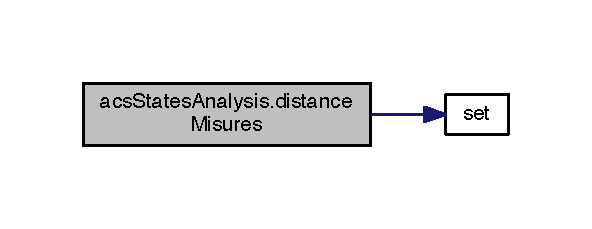
\includegraphics[width=284pt]{a00104_a76768d52780b1415a920dc94b3c991c0_cgraph}
\end{center}
\end{figure}


\hypertarget{a00104_ad7c75c1e146fa51da42274cf7d5747d0}{\index{acs\-States\-Analysis@{acs\-States\-Analysis}!return\-Zero\-Species\-List@{return\-Zero\-Species\-List}}
\index{return\-Zero\-Species\-List@{return\-Zero\-Species\-List}!acsStatesAnalysis@{acs\-States\-Analysis}}
\subsubsection[{return\-Zero\-Species\-List}]{\setlength{\rightskip}{0pt plus 5cm}def acs\-States\-Analysis.\-return\-Zero\-Species\-List (
\begin{DoxyParamCaption}
\item[{}]{tmp\-Last\-Species\-File}
\end{DoxyParamCaption}
)}}\label{a00104_ad7c75c1e146fa51da42274cf7d5747d0}
\begin{DoxyVerb}Function to create a zero vector for each species (NO COMPLEXES)\end{DoxyVerb}
 

Definition at line 31 of file acs\-States\-Analysis.\-py.

\hypertarget{a00104_aeeb6d629132a9755b45a3008d445419c}{\index{acs\-States\-Analysis@{acs\-States\-Analysis}!zero\-Before\-Str\-Num@{zero\-Before\-Str\-Num}}
\index{zero\-Before\-Str\-Num@{zero\-Before\-Str\-Num}!acsStatesAnalysis@{acs\-States\-Analysis}}
\subsubsection[{zero\-Before\-Str\-Num}]{\setlength{\rightskip}{0pt plus 5cm}def acs\-States\-Analysis.\-zero\-Before\-Str\-Num (
\begin{DoxyParamCaption}
\item[{}]{tmpl, }
\item[{}]{tmp\-L}
\end{DoxyParamCaption}
)}}\label{a00104_aeeb6d629132a9755b45a3008d445419c}
\begin{DoxyVerb}Function to create string zero string vector before graph filename.
According to the total number of reactions N zeros will be add before the instant reaction number 
(e.g. reaction 130 of 10000 the string became '00130')\end{DoxyVerb}
 

Definition at line 21 of file acs\-States\-Analysis.\-py.



\subsection{Variable Documentation}
\hypertarget{a00104_aa5eb16eef2c90e2ccc991eb176280f21}{\index{acs\-States\-Analysis@{acs\-States\-Analysis}!A\-N\-G\-\_\-middle\-Previous\-F\-I\-L\-E\-\_\-\-F\-I\-D@{A\-N\-G\-\_\-middle\-Previous\-F\-I\-L\-E\-\_\-\-F\-I\-D}}
\index{A\-N\-G\-\_\-middle\-Previous\-F\-I\-L\-E\-\_\-\-F\-I\-D@{A\-N\-G\-\_\-middle\-Previous\-F\-I\-L\-E\-\_\-\-F\-I\-D}!acsStatesAnalysis@{acs\-States\-Analysis}}
\subsubsection[{A\-N\-G\-\_\-middle\-Previous\-F\-I\-L\-E\-\_\-\-F\-I\-D}]{\setlength{\rightskip}{0pt plus 5cm}tuple acs\-States\-Analysis.\-A\-N\-G\-\_\-middle\-Previous\-F\-I\-L\-E\-\_\-\-F\-I\-D = open('S\-T\-A\-T\-\_\-\-A\-N\-G\-\_\-t\-\_\-middle\-\_\-\-N\-O\-I\-N\-F\-L\-U\-X.\-csv', 'w')}}\label{a00104_aa5eb16eef2c90e2ccc991eb176280f21}


Definition at line 140 of file acs\-States\-Analysis.\-py.

\hypertarget{a00104_a68c23cb79e89d9e14acf9ed09f46f0e4}{\index{acs\-States\-Analysis@{acs\-States\-Analysis}!biodeversity\-F\-I\-D@{biodeversity\-F\-I\-D}}
\index{biodeversity\-F\-I\-D@{biodeversity\-F\-I\-D}!acsStatesAnalysis@{acs\-States\-Analysis}}
\subsubsection[{biodeversity\-F\-I\-D}]{\setlength{\rightskip}{0pt plus 5cm}tuple acs\-States\-Analysis.\-biodeversity\-F\-I\-D = open('S\-T\-A\-T\-\_\-\-G\-E\-N\-E\-R\-A\-L\-\_\-bio\-Diversity.\-csv', 'w')}}\label{a00104_a68c23cb79e89d9e14acf9ed09f46f0e4}


Definition at line 168 of file acs\-States\-Analysis.\-py.

\hypertarget{a00104_a247328d05f06695b0c2de9a001ca4548}{\index{acs\-States\-Analysis@{acs\-States\-Analysis}!bio\-Div\-Ind@{bio\-Div\-Ind}}
\index{bio\-Div\-Ind@{bio\-Div\-Ind}!acsStatesAnalysis@{acs\-States\-Analysis}}
\subsubsection[{bio\-Div\-Ind}]{\setlength{\rightskip}{0pt plus 5cm}tuple acs\-States\-Analysis.\-bio\-Div\-Ind = 0}}\label{a00104_a247328d05f06695b0c2de9a001ca4548}


Definition at line 273 of file acs\-States\-Analysis.\-py.

\hypertarget{a00104_ace41560d233dff88c3073be734bae944}{\index{acs\-States\-Analysis@{acs\-States\-Analysis}!complex\-\_\-\-F\-I\-D@{complex\-\_\-\-F\-I\-D}}
\index{complex\-\_\-\-F\-I\-D@{complex\-\_\-\-F\-I\-D}!acsStatesAnalysis@{acs\-States\-Analysis}}
\subsubsection[{complex\-\_\-\-F\-I\-D}]{\setlength{\rightskip}{0pt plus 5cm}tuple acs\-States\-Analysis.\-complex\-\_\-\-F\-I\-D = open('S\-T\-A\-T\-\_\-\-G\-E\-N\-E\-R\-A\-L\-\_\-complex.\-csv', 'w')}}\label{a00104_ace41560d233dff88c3073be734bae944}


Definition at line 164 of file acs\-States\-Analysis.\-py.

\hypertarget{a00104_a2ef28958c50aabe7867b32f8dd6f4ace}{\index{acs\-States\-Analysis@{acs\-States\-Analysis}!complex\-Mols\-\_\-\-F\-I\-D@{complex\-Mols\-\_\-\-F\-I\-D}}
\index{complex\-Mols\-\_\-\-F\-I\-D@{complex\-Mols\-\_\-\-F\-I\-D}!acsStatesAnalysis@{acs\-States\-Analysis}}
\subsubsection[{complex\-Mols\-\_\-\-F\-I\-D}]{\setlength{\rightskip}{0pt plus 5cm}tuple acs\-States\-Analysis.\-complex\-Mols\-\_\-\-F\-I\-D = open('S\-T\-A\-T\-\_\-\-G\-E\-N\-E\-R\-A\-L\-\_\-complex\-Mols.\-csv', 'w')}}\label{a00104_a2ef28958c50aabe7867b32f8dd6f4ace}


Definition at line 165 of file acs\-States\-Analysis.\-py.

\hypertarget{a00104_a15f99c617a2dc95e52f741ee99e71b7a}{\index{acs\-States\-Analysis@{acs\-States\-Analysis}!conc\-O\-L\-D@{conc\-O\-L\-D}}
\index{conc\-O\-L\-D@{conc\-O\-L\-D}!acsStatesAnalysis@{acs\-States\-Analysis}}
\subsubsection[{conc\-O\-L\-D}]{\setlength{\rightskip}{0pt plus 5cm}list acs\-States\-Analysis.\-conc\-O\-L\-D = {\bf conc}\mbox{[}\-:\mbox{]}}}\label{a00104_a15f99c617a2dc95e52f741ee99e71b7a}


Definition at line 351 of file acs\-States\-Analysis.\-py.

\hypertarget{a00104_ae98225d5c8c20399f5c3b888fa37746f}{\index{acs\-States\-Analysis@{acs\-States\-Analysis}!current\-Dir@{current\-Dir}}
\index{current\-Dir@{current\-Dir}!acsStatesAnalysis@{acs\-States\-Analysis}}
\subsubsection[{current\-Dir}]{\setlength{\rightskip}{0pt plus 5cm}string acs\-States\-Analysis.\-current\-Dir = ''}}\label{a00104_ae98225d5c8c20399f5c3b888fa37746f}


Definition at line 113 of file acs\-States\-Analysis.\-py.

\hypertarget{a00104_a555117703c3245ec7d3d73f5d991c8c5}{\index{acs\-States\-Analysis@{acs\-States\-Analysis}!delta\-Nspecies@{delta\-Nspecies}}
\index{delta\-Nspecies@{delta\-Nspecies}!acsStatesAnalysis@{acs\-States\-Analysis}}
\subsubsection[{delta\-Nspecies}]{\setlength{\rightskip}{0pt plus 5cm}acs\-States\-Analysis.\-delta\-Nspecies = number\-Of\-Species-\/{\bf old\-Number\-Of\-Species}}}\label{a00104_a555117703c3245ec7d3d73f5d991c8c5}


Definition at line 279 of file acs\-States\-Analysis.\-py.

\hypertarget{a00104_afcb9ec3ed11cfcacae8f796af7605425}{\index{acs\-States\-Analysis@{acs\-States\-Analysis}!E\-U\-C\-\_\-middle\-Previous\-F\-I\-L\-E\-\_\-\-F\-I\-D@{E\-U\-C\-\_\-middle\-Previous\-F\-I\-L\-E\-\_\-\-F\-I\-D}}
\index{E\-U\-C\-\_\-middle\-Previous\-F\-I\-L\-E\-\_\-\-F\-I\-D@{E\-U\-C\-\_\-middle\-Previous\-F\-I\-L\-E\-\_\-\-F\-I\-D}!acsStatesAnalysis@{acs\-States\-Analysis}}
\subsubsection[{E\-U\-C\-\_\-middle\-Previous\-F\-I\-L\-E\-\_\-\-F\-I\-D}]{\setlength{\rightskip}{0pt plus 5cm}tuple acs\-States\-Analysis.\-E\-U\-C\-\_\-middle\-Previous\-F\-I\-L\-E\-\_\-\-F\-I\-D = open('S\-T\-A\-T\-\_\-\-E\-U\-C\-\_\-t\-\_\-middle\-\_\-\-N\-O\-I\-N\-F\-L\-U\-X.\-csv', 'w')}}\label{a00104_afcb9ec3ed11cfcacae8f796af7605425}


Definition at line 142 of file acs\-States\-Analysis.\-py.

\hypertarget{a00104_a3548edac9afffda077dcbd2876616b39}{\index{acs\-States\-Analysis@{acs\-States\-Analysis}!E\-U\-C\-\_\-previous\-F\-I\-L\-E\-\_\-\-F\-I\-D@{E\-U\-C\-\_\-previous\-F\-I\-L\-E\-\_\-\-F\-I\-D}}
\index{E\-U\-C\-\_\-previous\-F\-I\-L\-E\-\_\-\-F\-I\-D@{E\-U\-C\-\_\-previous\-F\-I\-L\-E\-\_\-\-F\-I\-D}!acsStatesAnalysis@{acs\-States\-Analysis}}
\subsubsection[{E\-U\-C\-\_\-previous\-F\-I\-L\-E\-\_\-\-F\-I\-D}]{\setlength{\rightskip}{0pt plus 5cm}tuple acs\-States\-Analysis.\-E\-U\-C\-\_\-previous\-F\-I\-L\-E\-\_\-\-F\-I\-D = open('S\-T\-A\-T\-\_\-\-E\-U\-C\-\_\-t\-\_\-tminus\-\_\-1.\-csv', 'w')}}\label{a00104_a3548edac9afffda077dcbd2876616b39}


Definition at line 135 of file acs\-States\-Analysis.\-py.

\hypertarget{a00104_adf079c2d443f89f00a330a58f99c2095}{\index{acs\-States\-Analysis@{acs\-States\-Analysis}!E\-U\-C\-\_\-previous\-F\-I\-L\-E\-\_\-\-F\-I\-D\-\_\-group@{E\-U\-C\-\_\-previous\-F\-I\-L\-E\-\_\-\-F\-I\-D\-\_\-group}}
\index{E\-U\-C\-\_\-previous\-F\-I\-L\-E\-\_\-\-F\-I\-D\-\_\-group@{E\-U\-C\-\_\-previous\-F\-I\-L\-E\-\_\-\-F\-I\-D\-\_\-group}!acsStatesAnalysis@{acs\-States\-Analysis}}
\subsubsection[{E\-U\-C\-\_\-previous\-F\-I\-L\-E\-\_\-\-F\-I\-D\-\_\-group}]{\setlength{\rightskip}{0pt plus 5cm}tuple acs\-States\-Analysis.\-E\-U\-C\-\_\-previous\-F\-I\-L\-E\-\_\-\-F\-I\-D\-\_\-group = open('S\-T\-A\-T\-\_\-\-E\-U\-C\-\_\-t\-\_\-tminus\-\_\-1\-\_\-group.\-csv', 'w')}}\label{a00104_adf079c2d443f89f00a330a58f99c2095}


Definition at line 154 of file acs\-States\-Analysis.\-py.

\hypertarget{a00104_aa2efc59329473a7bbeaf3ce32ec4dc3d}{\index{acs\-States\-Analysis@{acs\-States\-Analysis}!E\-U\-C\-\_\-previous\-N\-O\-I\-N\-F\-L\-U\-X\-\_\-\-F\-I\-L\-E\-\_\-\-F\-I\-D@{E\-U\-C\-\_\-previous\-N\-O\-I\-N\-F\-L\-U\-X\-\_\-\-F\-I\-L\-E\-\_\-\-F\-I\-D}}
\index{E\-U\-C\-\_\-previous\-N\-O\-I\-N\-F\-L\-U\-X\-\_\-\-F\-I\-L\-E\-\_\-\-F\-I\-D@{E\-U\-C\-\_\-previous\-N\-O\-I\-N\-F\-L\-U\-X\-\_\-\-F\-I\-L\-E\-\_\-\-F\-I\-D}!acsStatesAnalysis@{acs\-States\-Analysis}}
\subsubsection[{E\-U\-C\-\_\-previous\-N\-O\-I\-N\-F\-L\-U\-X\-\_\-\-F\-I\-L\-E\-\_\-\-F\-I\-D}]{\setlength{\rightskip}{0pt plus 5cm}tuple acs\-States\-Analysis.\-E\-U\-C\-\_\-previous\-N\-O\-I\-N\-F\-L\-U\-X\-\_\-\-F\-I\-L\-E\-\_\-\-F\-I\-D = open('S\-T\-A\-T\-\_\-\-E\-U\-C\-\_\-t\-\_\-tminus\-\_\-1\-\_\-\-N\-O\-I\-N\-F\-L\-U\-X.\-csv', 'w')}}\label{a00104_aa2efc59329473a7bbeaf3ce32ec4dc3d}


Definition at line 136 of file acs\-States\-Analysis.\-py.

\hypertarget{a00104_ace5cf628b305f9110e058d7dafd27fb4}{\index{acs\-States\-Analysis@{acs\-States\-Analysis}!E\-U\-C\-\_\-previous\-N\-O\-I\-N\-F\-L\-U\-X\-\_\-\-F\-I\-L\-E\-\_\-\-F\-I\-D\-\_\-group@{E\-U\-C\-\_\-previous\-N\-O\-I\-N\-F\-L\-U\-X\-\_\-\-F\-I\-L\-E\-\_\-\-F\-I\-D\-\_\-group}}
\index{E\-U\-C\-\_\-previous\-N\-O\-I\-N\-F\-L\-U\-X\-\_\-\-F\-I\-L\-E\-\_\-\-F\-I\-D\-\_\-group@{E\-U\-C\-\_\-previous\-N\-O\-I\-N\-F\-L\-U\-X\-\_\-\-F\-I\-L\-E\-\_\-\-F\-I\-D\-\_\-group}!acsStatesAnalysis@{acs\-States\-Analysis}}
\subsubsection[{E\-U\-C\-\_\-previous\-N\-O\-I\-N\-F\-L\-U\-X\-\_\-\-F\-I\-L\-E\-\_\-\-F\-I\-D\-\_\-group}]{\setlength{\rightskip}{0pt plus 5cm}tuple acs\-States\-Analysis.\-E\-U\-C\-\_\-previous\-N\-O\-I\-N\-F\-L\-U\-X\-\_\-\-F\-I\-L\-E\-\_\-\-F\-I\-D\-\_\-group = open('S\-T\-A\-T\-\_\-\-E\-U\-C\-\_\-t\-\_\-tminus\-\_\-1\-\_\-\-N\-O\-I\-N\-F\-L\-U\-X\-\_\-group.\-csv', 'w')}}\label{a00104_ace5cf628b305f9110e058d7dafd27fb4}


Definition at line 155 of file acs\-States\-Analysis.\-py.

\hypertarget{a00104_a3d812ff298612e6aae54e7a9abfddbf2}{\index{acs\-States\-Analysis@{acs\-States\-Analysis}!E\-U\-C\-\_\-start\-F\-I\-L\-E\-\_\-\-F\-I\-D@{E\-U\-C\-\_\-start\-F\-I\-L\-E\-\_\-\-F\-I\-D}}
\index{E\-U\-C\-\_\-start\-F\-I\-L\-E\-\_\-\-F\-I\-D@{E\-U\-C\-\_\-start\-F\-I\-L\-E\-\_\-\-F\-I\-D}!acsStatesAnalysis@{acs\-States\-Analysis}}
\subsubsection[{E\-U\-C\-\_\-start\-F\-I\-L\-E\-\_\-\-F\-I\-D}]{\setlength{\rightskip}{0pt plus 5cm}tuple acs\-States\-Analysis.\-E\-U\-C\-\_\-start\-F\-I\-L\-E\-\_\-\-F\-I\-D = open('S\-T\-A\-T\-\_\-\-E\-U\-C\-\_\-t\-\_\-start.\-csv', 'w')}}\label{a00104_a3d812ff298612e6aae54e7a9abfddbf2}


Definition at line 137 of file acs\-States\-Analysis.\-py.

\hypertarget{a00104_abe1a2acadc97e46d55c6f4164c0890dc}{\index{acs\-States\-Analysis@{acs\-States\-Analysis}!E\-U\-C\-\_\-start\-F\-I\-L\-E\-\_\-\-F\-I\-D\-\_\-group@{E\-U\-C\-\_\-start\-F\-I\-L\-E\-\_\-\-F\-I\-D\-\_\-group}}
\index{E\-U\-C\-\_\-start\-F\-I\-L\-E\-\_\-\-F\-I\-D\-\_\-group@{E\-U\-C\-\_\-start\-F\-I\-L\-E\-\_\-\-F\-I\-D\-\_\-group}!acsStatesAnalysis@{acs\-States\-Analysis}}
\subsubsection[{E\-U\-C\-\_\-start\-F\-I\-L\-E\-\_\-\-F\-I\-D\-\_\-group}]{\setlength{\rightskip}{0pt plus 5cm}tuple acs\-States\-Analysis.\-E\-U\-C\-\_\-start\-F\-I\-L\-E\-\_\-\-F\-I\-D\-\_\-group = open('S\-T\-A\-T\-\_\-\-E\-U\-C\-\_\-t\-\_\-start\-\_\-group.\-csv', 'w')}}\label{a00104_abe1a2acadc97e46d55c6f4164c0890dc}


Definition at line 156 of file acs\-States\-Analysis.\-py.

\hypertarget{a00104_a8ae5873fd9b162495a512e314047e930}{\index{acs\-States\-Analysis@{acs\-States\-Analysis}!E\-U\-C\-\_\-start\-N\-O\-I\-N\-F\-L\-U\-X\-\_\-\-F\-I\-L\-E\-\_\-\-F\-I\-D@{E\-U\-C\-\_\-start\-N\-O\-I\-N\-F\-L\-U\-X\-\_\-\-F\-I\-L\-E\-\_\-\-F\-I\-D}}
\index{E\-U\-C\-\_\-start\-N\-O\-I\-N\-F\-L\-U\-X\-\_\-\-F\-I\-L\-E\-\_\-\-F\-I\-D@{E\-U\-C\-\_\-start\-N\-O\-I\-N\-F\-L\-U\-X\-\_\-\-F\-I\-L\-E\-\_\-\-F\-I\-D}!acsStatesAnalysis@{acs\-States\-Analysis}}
\subsubsection[{E\-U\-C\-\_\-start\-N\-O\-I\-N\-F\-L\-U\-X\-\_\-\-F\-I\-L\-E\-\_\-\-F\-I\-D}]{\setlength{\rightskip}{0pt plus 5cm}tuple acs\-States\-Analysis.\-E\-U\-C\-\_\-start\-N\-O\-I\-N\-F\-L\-U\-X\-\_\-\-F\-I\-L\-E\-\_\-\-F\-I\-D = open('S\-T\-A\-T\-\_\-\-E\-U\-C\-\_\-t\-\_\-start\-\_\-\-N\-O\-I\-N\-F\-L\-U\-X.\-csv', 'w')}}\label{a00104_a8ae5873fd9b162495a512e314047e930}


Definition at line 138 of file acs\-States\-Analysis.\-py.

\hypertarget{a00104_aef08a333d5fed02e90483cc87e389ed0}{\index{acs\-States\-Analysis@{acs\-States\-Analysis}!E\-U\-C\-\_\-start\-N\-O\-I\-N\-F\-L\-U\-X\-\_\-\-F\-I\-L\-E\-\_\-\-F\-I\-D\-\_\-group@{E\-U\-C\-\_\-start\-N\-O\-I\-N\-F\-L\-U\-X\-\_\-\-F\-I\-L\-E\-\_\-\-F\-I\-D\-\_\-group}}
\index{E\-U\-C\-\_\-start\-N\-O\-I\-N\-F\-L\-U\-X\-\_\-\-F\-I\-L\-E\-\_\-\-F\-I\-D\-\_\-group@{E\-U\-C\-\_\-start\-N\-O\-I\-N\-F\-L\-U\-X\-\_\-\-F\-I\-L\-E\-\_\-\-F\-I\-D\-\_\-group}!acsStatesAnalysis@{acs\-States\-Analysis}}
\subsubsection[{E\-U\-C\-\_\-start\-N\-O\-I\-N\-F\-L\-U\-X\-\_\-\-F\-I\-L\-E\-\_\-\-F\-I\-D\-\_\-group}]{\setlength{\rightskip}{0pt plus 5cm}tuple acs\-States\-Analysis.\-E\-U\-C\-\_\-start\-N\-O\-I\-N\-F\-L\-U\-X\-\_\-\-F\-I\-L\-E\-\_\-\-F\-I\-D\-\_\-group = open('S\-T\-A\-T\-\_\-\-E\-U\-C\-\_\-t\-\_\-start\-\_\-\-N\-O\-I\-N\-F\-L\-U\-X\-\_\-group.\-csv', 'w')}}\label{a00104_aef08a333d5fed02e90483cc87e389ed0}


Definition at line 157 of file acs\-States\-Analysis.\-py.

\hypertarget{a00104_a2cc9b964c81489c25978be53ab38eb16}{\index{acs\-States\-Analysis@{acs\-States\-Analysis}!evaluated\-F\-I\-D@{evaluated\-F\-I\-D}}
\index{evaluated\-F\-I\-D@{evaluated\-F\-I\-D}!acsStatesAnalysis@{acs\-States\-Analysis}}
\subsubsection[{evaluated\-F\-I\-D}]{\setlength{\rightskip}{0pt plus 5cm}tuple acs\-States\-Analysis.\-evaluated\-F\-I\-D = open('S\-T\-A\-T\-\_\-\-G\-E\-N\-E\-R\-A\-L\-\_\-evaluated.\-csv', 'w')}}\label{a00104_a2cc9b964c81489c25978be53ab38eb16}


Definition at line 166 of file acs\-States\-Analysis.\-py.

\hypertarget{a00104_afd34aa2ef2c410c2d71007bac0a121fd}{\index{acs\-States\-Analysis@{acs\-States\-Analysis}!fid\-Species@{fid\-Species}}
\index{fid\-Species@{fid\-Species}!acsStatesAnalysis@{acs\-States\-Analysis}}
\subsubsection[{fid\-Species}]{\setlength{\rightskip}{0pt plus 5cm}tuple acs\-States\-Analysis.\-fid\-Species = open(sng\-Species\-File, '{\bf r}')}}\label{a00104_afd34aa2ef2c410c2d71007bac0a121fd}


Definition at line 230 of file acs\-States\-Analysis.\-py.

\hypertarget{a00104_a69b59a10e5dc62a6e0d5325e9a27e5c6}{\index{acs\-States\-Analysis@{acs\-States\-Analysis}!filename@{filename}}
\index{filename@{filename}!acsStatesAnalysis@{acs\-States\-Analysis}}
\subsubsection[{filename}]{\setlength{\rightskip}{0pt plus 5cm}string acs\-States\-Analysis.\-filename = \char`\"{}S\-T\-A\-T\-\_\-species\-\_\-\-Concentrations\-\_\-\char`\"{}}}\label{a00104_a69b59a10e5dc62a6e0d5325e9a27e5c6}


Definition at line 410 of file acs\-States\-Analysis.\-py.

\hypertarget{a00104_a1dd2f2c85f697e454c99be1a157d6c17}{\index{acs\-States\-Analysis@{acs\-States\-Analysis}!group\-\_\-\-A\-\_\-prev@{group\-\_\-\-A\-\_\-prev}}
\index{group\-\_\-\-A\-\_\-prev@{group\-\_\-\-A\-\_\-prev}!acsStatesAnalysis@{acs\-States\-Analysis}}
\subsubsection[{group\-\_\-\-A\-\_\-prev}]{\setlength{\rightskip}{0pt plus 5cm}list acs\-States\-Analysis.\-group\-\_\-\-A\-\_\-prev = \mbox{[}$\,$\mbox{]}}}\label{a00104_a1dd2f2c85f697e454c99be1a157d6c17}


Definition at line 186 of file acs\-States\-Analysis.\-py.

\hypertarget{a00104_a4d77133a6a303d9486944707f3310cf8}{\index{acs\-States\-Analysis@{acs\-States\-Analysis}!group\-\_\-\-A\-\_\-prev\-\_\-\-N\-I@{group\-\_\-\-A\-\_\-prev\-\_\-\-N\-I}}
\index{group\-\_\-\-A\-\_\-prev\-\_\-\-N\-I@{group\-\_\-\-A\-\_\-prev\-\_\-\-N\-I}!acsStatesAnalysis@{acs\-States\-Analysis}}
\subsubsection[{group\-\_\-\-A\-\_\-prev\-\_\-\-N\-I}]{\setlength{\rightskip}{0pt plus 5cm}list acs\-States\-Analysis.\-group\-\_\-\-A\-\_\-prev\-\_\-\-N\-I = \mbox{[}$\,$\mbox{]}}}\label{a00104_a4d77133a6a303d9486944707f3310cf8}


Definition at line 188 of file acs\-States\-Analysis.\-py.

\hypertarget{a00104_a3898175300d001a17a60c23656d2812f}{\index{acs\-States\-Analysis@{acs\-States\-Analysis}!group\-\_\-\-A\-\_\-start@{group\-\_\-\-A\-\_\-start}}
\index{group\-\_\-\-A\-\_\-start@{group\-\_\-\-A\-\_\-start}!acsStatesAnalysis@{acs\-States\-Analysis}}
\subsubsection[{group\-\_\-\-A\-\_\-start}]{\setlength{\rightskip}{0pt plus 5cm}list acs\-States\-Analysis.\-group\-\_\-\-A\-\_\-start = \mbox{[}$\,$\mbox{]}}}\label{a00104_a3898175300d001a17a60c23656d2812f}


Definition at line 187 of file acs\-States\-Analysis.\-py.

\hypertarget{a00104_aedb746884c5ae6e301c8ad2d8307fe4d}{\index{acs\-States\-Analysis@{acs\-States\-Analysis}!group\-\_\-\-A\-\_\-start\-\_\-\-N\-I@{group\-\_\-\-A\-\_\-start\-\_\-\-N\-I}}
\index{group\-\_\-\-A\-\_\-start\-\_\-\-N\-I@{group\-\_\-\-A\-\_\-start\-\_\-\-N\-I}!acsStatesAnalysis@{acs\-States\-Analysis}}
\subsubsection[{group\-\_\-\-A\-\_\-start\-\_\-\-N\-I}]{\setlength{\rightskip}{0pt plus 5cm}list acs\-States\-Analysis.\-group\-\_\-\-A\-\_\-start\-\_\-\-N\-I = \mbox{[}$\,$\mbox{]}}}\label{a00104_aedb746884c5ae6e301c8ad2d8307fe4d}


Definition at line 189 of file acs\-States\-Analysis.\-py.

\hypertarget{a00104_aaf0dd6e74d88a7cf2e909301b422c17d}{\index{acs\-States\-Analysis@{acs\-States\-Analysis}!H\-A\-M\-\_\-middle\-Previous\-F\-I\-L\-E\-\_\-\-F\-I\-D@{H\-A\-M\-\_\-middle\-Previous\-F\-I\-L\-E\-\_\-\-F\-I\-D}}
\index{H\-A\-M\-\_\-middle\-Previous\-F\-I\-L\-E\-\_\-\-F\-I\-D@{H\-A\-M\-\_\-middle\-Previous\-F\-I\-L\-E\-\_\-\-F\-I\-D}!acsStatesAnalysis@{acs\-States\-Analysis}}
\subsubsection[{H\-A\-M\-\_\-middle\-Previous\-F\-I\-L\-E\-\_\-\-F\-I\-D}]{\setlength{\rightskip}{0pt plus 5cm}tuple acs\-States\-Analysis.\-H\-A\-M\-\_\-middle\-Previous\-F\-I\-L\-E\-\_\-\-F\-I\-D = open('S\-T\-A\-T\-\_\-\-H\-A\-M\-\_\-t\-\_\-middle\-\_\-\-N\-O\-I\-N\-F\-L\-U\-X.\-csv', 'w')}}\label{a00104_aaf0dd6e74d88a7cf2e909301b422c17d}


Definition at line 141 of file acs\-States\-Analysis.\-py.

\hypertarget{a00104_a3aad86d2cdbfb6f36b4b563b190d76c9}{\index{acs\-States\-Analysis@{acs\-States\-Analysis}!H\-A\-M\-\_\-previous\-F\-I\-L\-E\-\_\-\-F\-I\-D@{H\-A\-M\-\_\-previous\-F\-I\-L\-E\-\_\-\-F\-I\-D}}
\index{H\-A\-M\-\_\-previous\-F\-I\-L\-E\-\_\-\-F\-I\-D@{H\-A\-M\-\_\-previous\-F\-I\-L\-E\-\_\-\-F\-I\-D}!acsStatesAnalysis@{acs\-States\-Analysis}}
\subsubsection[{H\-A\-M\-\_\-previous\-F\-I\-L\-E\-\_\-\-F\-I\-D}]{\setlength{\rightskip}{0pt plus 5cm}tuple acs\-States\-Analysis.\-H\-A\-M\-\_\-previous\-F\-I\-L\-E\-\_\-\-F\-I\-D = open('S\-T\-A\-T\-\_\-\-H\-A\-M\-\_\-t\-\_\-tminus\-\_\-1.\-csv', 'w')}}\label{a00104_a3aad86d2cdbfb6f36b4b563b190d76c9}


Definition at line 130 of file acs\-States\-Analysis.\-py.

\hypertarget{a00104_aa72272e636b1eafe39ed3367145433f2}{\index{acs\-States\-Analysis@{acs\-States\-Analysis}!H\-A\-M\-\_\-previous\-F\-I\-L\-E\-\_\-\-F\-I\-D\-\_\-group@{H\-A\-M\-\_\-previous\-F\-I\-L\-E\-\_\-\-F\-I\-D\-\_\-group}}
\index{H\-A\-M\-\_\-previous\-F\-I\-L\-E\-\_\-\-F\-I\-D\-\_\-group@{H\-A\-M\-\_\-previous\-F\-I\-L\-E\-\_\-\-F\-I\-D\-\_\-group}!acsStatesAnalysis@{acs\-States\-Analysis}}
\subsubsection[{H\-A\-M\-\_\-previous\-F\-I\-L\-E\-\_\-\-F\-I\-D\-\_\-group}]{\setlength{\rightskip}{0pt plus 5cm}tuple acs\-States\-Analysis.\-H\-A\-M\-\_\-previous\-F\-I\-L\-E\-\_\-\-F\-I\-D\-\_\-group = open('S\-T\-A\-T\-\_\-\-H\-A\-M\-\_\-t\-\_\-tminus\-\_\-1\-\_\-group.\-csv', 'w')}}\label{a00104_aa72272e636b1eafe39ed3367145433f2}


Definition at line 149 of file acs\-States\-Analysis.\-py.

\hypertarget{a00104_a621d86851e86f9c83bb0add9ec741d7f}{\index{acs\-States\-Analysis@{acs\-States\-Analysis}!H\-A\-M\-\_\-previous\-N\-O\-I\-N\-F\-L\-U\-X\-\_\-\-F\-I\-L\-E\-\_\-\-F\-I\-D@{H\-A\-M\-\_\-previous\-N\-O\-I\-N\-F\-L\-U\-X\-\_\-\-F\-I\-L\-E\-\_\-\-F\-I\-D}}
\index{H\-A\-M\-\_\-previous\-N\-O\-I\-N\-F\-L\-U\-X\-\_\-\-F\-I\-L\-E\-\_\-\-F\-I\-D@{H\-A\-M\-\_\-previous\-N\-O\-I\-N\-F\-L\-U\-X\-\_\-\-F\-I\-L\-E\-\_\-\-F\-I\-D}!acsStatesAnalysis@{acs\-States\-Analysis}}
\subsubsection[{H\-A\-M\-\_\-previous\-N\-O\-I\-N\-F\-L\-U\-X\-\_\-\-F\-I\-L\-E\-\_\-\-F\-I\-D}]{\setlength{\rightskip}{0pt plus 5cm}tuple acs\-States\-Analysis.\-H\-A\-M\-\_\-previous\-N\-O\-I\-N\-F\-L\-U\-X\-\_\-\-F\-I\-L\-E\-\_\-\-F\-I\-D = open('S\-T\-A\-T\-\_\-\-H\-A\-M\-\_\-t\-\_\-tminus\-\_\-1\-\_\-\-N\-O\-I\-N\-F\-L\-U\-X.\-csv', 'w')}}\label{a00104_a621d86851e86f9c83bb0add9ec741d7f}


Definition at line 131 of file acs\-States\-Analysis.\-py.

\hypertarget{a00104_a092676cc95ddff57aac2aa077ce22d52}{\index{acs\-States\-Analysis@{acs\-States\-Analysis}!H\-A\-M\-\_\-previous\-N\-O\-I\-N\-F\-L\-U\-X\-\_\-\-F\-I\-L\-E\-\_\-\-F\-I\-D\-\_\-group@{H\-A\-M\-\_\-previous\-N\-O\-I\-N\-F\-L\-U\-X\-\_\-\-F\-I\-L\-E\-\_\-\-F\-I\-D\-\_\-group}}
\index{H\-A\-M\-\_\-previous\-N\-O\-I\-N\-F\-L\-U\-X\-\_\-\-F\-I\-L\-E\-\_\-\-F\-I\-D\-\_\-group@{H\-A\-M\-\_\-previous\-N\-O\-I\-N\-F\-L\-U\-X\-\_\-\-F\-I\-L\-E\-\_\-\-F\-I\-D\-\_\-group}!acsStatesAnalysis@{acs\-States\-Analysis}}
\subsubsection[{H\-A\-M\-\_\-previous\-N\-O\-I\-N\-F\-L\-U\-X\-\_\-\-F\-I\-L\-E\-\_\-\-F\-I\-D\-\_\-group}]{\setlength{\rightskip}{0pt plus 5cm}tuple acs\-States\-Analysis.\-H\-A\-M\-\_\-previous\-N\-O\-I\-N\-F\-L\-U\-X\-\_\-\-F\-I\-L\-E\-\_\-\-F\-I\-D\-\_\-group = open('S\-T\-A\-T\-\_\-\-H\-A\-M\-\_\-t\-\_\-tminus\-\_\-1\-\_\-\-N\-O\-I\-N\-F\-L\-U\-X\-\_\-group.\-csv', 'w')}}\label{a00104_a092676cc95ddff57aac2aa077ce22d52}


Definition at line 150 of file acs\-States\-Analysis.\-py.

\hypertarget{a00104_abb14887e587e1107fc13046ad313077e}{\index{acs\-States\-Analysis@{acs\-States\-Analysis}!H\-A\-M\-\_\-start\-F\-I\-L\-E\-\_\-\-F\-I\-D@{H\-A\-M\-\_\-start\-F\-I\-L\-E\-\_\-\-F\-I\-D}}
\index{H\-A\-M\-\_\-start\-F\-I\-L\-E\-\_\-\-F\-I\-D@{H\-A\-M\-\_\-start\-F\-I\-L\-E\-\_\-\-F\-I\-D}!acsStatesAnalysis@{acs\-States\-Analysis}}
\subsubsection[{H\-A\-M\-\_\-start\-F\-I\-L\-E\-\_\-\-F\-I\-D}]{\setlength{\rightskip}{0pt plus 5cm}tuple acs\-States\-Analysis.\-H\-A\-M\-\_\-start\-F\-I\-L\-E\-\_\-\-F\-I\-D = open('S\-T\-A\-T\-\_\-\-H\-A\-M\-\_\-t\-\_\-start.\-csv', 'w')}}\label{a00104_abb14887e587e1107fc13046ad313077e}


Definition at line 132 of file acs\-States\-Analysis.\-py.

\hypertarget{a00104_ab74ecb2bab6a84c44274814862f2e96c}{\index{acs\-States\-Analysis@{acs\-States\-Analysis}!H\-A\-M\-\_\-start\-F\-I\-L\-E\-\_\-\-F\-I\-D\-\_\-group@{H\-A\-M\-\_\-start\-F\-I\-L\-E\-\_\-\-F\-I\-D\-\_\-group}}
\index{H\-A\-M\-\_\-start\-F\-I\-L\-E\-\_\-\-F\-I\-D\-\_\-group@{H\-A\-M\-\_\-start\-F\-I\-L\-E\-\_\-\-F\-I\-D\-\_\-group}!acsStatesAnalysis@{acs\-States\-Analysis}}
\subsubsection[{H\-A\-M\-\_\-start\-F\-I\-L\-E\-\_\-\-F\-I\-D\-\_\-group}]{\setlength{\rightskip}{0pt plus 5cm}tuple acs\-States\-Analysis.\-H\-A\-M\-\_\-start\-F\-I\-L\-E\-\_\-\-F\-I\-D\-\_\-group = open('S\-T\-A\-T\-\_\-\-H\-A\-M\-\_\-t\-\_\-start\-\_\-group.\-csv', 'w')}}\label{a00104_ab74ecb2bab6a84c44274814862f2e96c}


Definition at line 151 of file acs\-States\-Analysis.\-py.

\hypertarget{a00104_ab8a3b402c0b418cc290889a5f6482280}{\index{acs\-States\-Analysis@{acs\-States\-Analysis}!H\-A\-M\-\_\-start\-N\-O\-I\-N\-F\-L\-U\-X\-\_\-\-F\-I\-L\-E\-\_\-\-F\-I\-D@{H\-A\-M\-\_\-start\-N\-O\-I\-N\-F\-L\-U\-X\-\_\-\-F\-I\-L\-E\-\_\-\-F\-I\-D}}
\index{H\-A\-M\-\_\-start\-N\-O\-I\-N\-F\-L\-U\-X\-\_\-\-F\-I\-L\-E\-\_\-\-F\-I\-D@{H\-A\-M\-\_\-start\-N\-O\-I\-N\-F\-L\-U\-X\-\_\-\-F\-I\-L\-E\-\_\-\-F\-I\-D}!acsStatesAnalysis@{acs\-States\-Analysis}}
\subsubsection[{H\-A\-M\-\_\-start\-N\-O\-I\-N\-F\-L\-U\-X\-\_\-\-F\-I\-L\-E\-\_\-\-F\-I\-D}]{\setlength{\rightskip}{0pt plus 5cm}tuple acs\-States\-Analysis.\-H\-A\-M\-\_\-start\-N\-O\-I\-N\-F\-L\-U\-X\-\_\-\-F\-I\-L\-E\-\_\-\-F\-I\-D = open('S\-T\-A\-T\-\_\-\-H\-A\-M\-\_\-t\-\_\-start\-\_\-\-N\-O\-I\-N\-F\-L\-U\-X.\-csv', 'w')}}\label{a00104_ab8a3b402c0b418cc290889a5f6482280}


Definition at line 133 of file acs\-States\-Analysis.\-py.

\hypertarget{a00104_a4652c6dad393663e40970d7f6422c1d6}{\index{acs\-States\-Analysis@{acs\-States\-Analysis}!H\-A\-M\-\_\-start\-N\-O\-I\-N\-F\-L\-U\-X\-\_\-\-F\-I\-L\-E\-\_\-\-F\-I\-D\-\_\-group@{H\-A\-M\-\_\-start\-N\-O\-I\-N\-F\-L\-U\-X\-\_\-\-F\-I\-L\-E\-\_\-\-F\-I\-D\-\_\-group}}
\index{H\-A\-M\-\_\-start\-N\-O\-I\-N\-F\-L\-U\-X\-\_\-\-F\-I\-L\-E\-\_\-\-F\-I\-D\-\_\-group@{H\-A\-M\-\_\-start\-N\-O\-I\-N\-F\-L\-U\-X\-\_\-\-F\-I\-L\-E\-\_\-\-F\-I\-D\-\_\-group}!acsStatesAnalysis@{acs\-States\-Analysis}}
\subsubsection[{H\-A\-M\-\_\-start\-N\-O\-I\-N\-F\-L\-U\-X\-\_\-\-F\-I\-L\-E\-\_\-\-F\-I\-D\-\_\-group}]{\setlength{\rightskip}{0pt plus 5cm}tuple acs\-States\-Analysis.\-H\-A\-M\-\_\-start\-N\-O\-I\-N\-F\-L\-U\-X\-\_\-\-F\-I\-L\-E\-\_\-\-F\-I\-D\-\_\-group = open('S\-T\-A\-T\-\_\-\-H\-A\-M\-\_\-t\-\_\-start\-\_\-\-N\-O\-I\-N\-F\-L\-U\-X\-\_\-group.\-csv', 'w')}}\label{a00104_a4652c6dad393663e40970d7f6422c1d6}


Definition at line 152 of file acs\-States\-Analysis.\-py.

\hypertarget{a00104_ab7bbe9440116d34c9a373c40fc59bb3d}{\index{acs\-States\-Analysis@{acs\-States\-Analysis}!living\-Species\-\_\-\-F\-I\-D@{living\-Species\-\_\-\-F\-I\-D}}
\index{living\-Species\-\_\-\-F\-I\-D@{living\-Species\-\_\-\-F\-I\-D}!acsStatesAnalysis@{acs\-States\-Analysis}}
\subsubsection[{living\-Species\-\_\-\-F\-I\-D}]{\setlength{\rightskip}{0pt plus 5cm}tuple acs\-States\-Analysis.\-living\-Species\-\_\-\-F\-I\-D = open('S\-T\-A\-T\-\_\-\-G\-E\-N\-E\-R\-A\-L\-\_\-living\-Species.\-csv', 'w')}}\label{a00104_ab7bbe9440116d34c9a373c40fc59bb3d}


Definition at line 160 of file acs\-States\-Analysis.\-py.

\hypertarget{a00104_a603a41889d8732146d44da83ffaf0489}{\index{acs\-States\-Analysis@{acs\-States\-Analysis}!mols\-\_\-\-F\-I\-D@{mols\-\_\-\-F\-I\-D}}
\index{mols\-\_\-\-F\-I\-D@{mols\-\_\-\-F\-I\-D}!acsStatesAnalysis@{acs\-States\-Analysis}}
\subsubsection[{mols\-\_\-\-F\-I\-D}]{\setlength{\rightskip}{0pt plus 5cm}tuple acs\-States\-Analysis.\-mols\-\_\-\-F\-I\-D = open('S\-T\-A\-T\-\_\-\-G\-E\-N\-E\-R\-A\-L\-\_\-mols.\-csv', 'w')}}\label{a00104_a603a41889d8732146d44da83ffaf0489}


Definition at line 161 of file acs\-States\-Analysis.\-py.

\hypertarget{a00104_a5e117df6e0cdffdae13947622c6c4890}{\index{acs\-States\-Analysis@{acs\-States\-Analysis}!ndn@{ndn}}
\index{ndn@{ndn}!acsStatesAnalysis@{acs\-States\-Analysis}}
\subsubsection[{ndn}]{\setlength{\rightskip}{0pt plus 5cm}string acs\-States\-Analysis.\-ndn = {\bf current\-Dir}+'\-\_\-0\-\_\-new\-\_\-all\-Stat\-Results'}}\label{a00104_a5e117df6e0cdffdae13947622c6c4890}


Definition at line 114 of file acs\-States\-Analysis.\-py.

\hypertarget{a00104_a62d6cfd52b4428ab7ea4d75d43b2d49b}{\index{acs\-States\-Analysis@{acs\-States\-Analysis}!newdir\-All\-Results@{newdir\-All\-Results}}
\index{newdir\-All\-Results@{newdir\-All\-Results}!acsStatesAnalysis@{acs\-States\-Analysis}}
\subsubsection[{newdir\-All\-Results}]{\setlength{\rightskip}{0pt plus 5cm}tuple acs\-States\-Analysis.\-newdir\-All\-Results = os.\-path.\-join(os.\-curdir, {\bf ndn})}}\label{a00104_a62d6cfd52b4428ab7ea4d75d43b2d49b}


Definition at line 115 of file acs\-States\-Analysis.\-py.

\hypertarget{a00104_abdb6e583333cc08cac8c63631db80b5b}{\index{acs\-States\-Analysis@{acs\-States\-Analysis}!new\-Species\-\_\-\-F\-I\-D@{new\-Species\-\_\-\-F\-I\-D}}
\index{new\-Species\-\_\-\-F\-I\-D@{new\-Species\-\_\-\-F\-I\-D}!acsStatesAnalysis@{acs\-States\-Analysis}}
\subsubsection[{new\-Species\-\_\-\-F\-I\-D}]{\setlength{\rightskip}{0pt plus 5cm}tuple acs\-States\-Analysis.\-new\-Species\-\_\-\-F\-I\-D = open('S\-T\-A\-T\-\_\-\-G\-E\-N\-E\-R\-A\-L\-\_\-new\-Species.\-csv', 'w')}}\label{a00104_abdb6e583333cc08cac8c63631db80b5b}


Definition at line 159 of file acs\-States\-Analysis.\-py.

\hypertarget{a00104_a54acb4eba0735e72c2a820383febd37f}{\index{acs\-States\-Analysis@{acs\-States\-Analysis}!number\-Of\-Gen@{number\-Of\-Gen}}
\index{number\-Of\-Gen@{number\-Of\-Gen}!acsStatesAnalysis@{acs\-States\-Analysis}}
\subsubsection[{number\-Of\-Gen}]{\setlength{\rightskip}{0pt plus 5cm}tuple acs\-States\-Analysis.\-number\-Of\-Gen = len(glob.\-glob(os.\-path.\-join({\bf res\-Dir\-Path},'times\-\_\-$\ast$')))}}\label{a00104_a54acb4eba0735e72c2a820383febd37f}


Definition at line 184 of file acs\-States\-Analysis.\-py.

\hypertarget{a00104_abe1ce9bb85ee916d2046efc5c3fe6b30}{\index{acs\-States\-Analysis@{acs\-States\-Analysis}!old\-Number\-Of\-Species@{old\-Number\-Of\-Species}}
\index{old\-Number\-Of\-Species@{old\-Number\-Of\-Species}!acsStatesAnalysis@{acs\-States\-Analysis}}
\subsubsection[{old\-Number\-Of\-Species}]{\setlength{\rightskip}{0pt plus 5cm}acs\-States\-Analysis.\-old\-Number\-Of\-Species = 0}}\label{a00104_abe1ce9bb85ee916d2046efc5c3fe6b30}


Definition at line 222 of file acs\-States\-Analysis.\-py.

\hypertarget{a00104_aba65725a1bd6d1b891b02dc7f3db2335}{\index{acs\-States\-Analysis@{acs\-States\-Analysis}!previous\-F\-I\-L\-E\-\_\-\-F\-I\-D@{previous\-F\-I\-L\-E\-\_\-\-F\-I\-D}}
\index{previous\-F\-I\-L\-E\-\_\-\-F\-I\-D@{previous\-F\-I\-L\-E\-\_\-\-F\-I\-D}!acsStatesAnalysis@{acs\-States\-Analysis}}
\subsubsection[{previous\-F\-I\-L\-E\-\_\-\-F\-I\-D}]{\setlength{\rightskip}{0pt plus 5cm}tuple acs\-States\-Analysis.\-previous\-F\-I\-L\-E\-\_\-\-F\-I\-D = open('S\-T\-A\-T\-\_\-t\-\_\-tminus\-\_\-1.\-csv', 'w')}}\label{a00104_aba65725a1bd6d1b891b02dc7f3db2335}


Definition at line 125 of file acs\-States\-Analysis.\-py.

\hypertarget{a00104_a9e72c152be1f5aac24af10b353b16390}{\index{acs\-States\-Analysis@{acs\-States\-Analysis}!previous\-F\-I\-L\-E\-\_\-\-F\-I\-D\-\_\-group@{previous\-F\-I\-L\-E\-\_\-\-F\-I\-D\-\_\-group}}
\index{previous\-F\-I\-L\-E\-\_\-\-F\-I\-D\-\_\-group@{previous\-F\-I\-L\-E\-\_\-\-F\-I\-D\-\_\-group}!acsStatesAnalysis@{acs\-States\-Analysis}}
\subsubsection[{previous\-F\-I\-L\-E\-\_\-\-F\-I\-D\-\_\-group}]{\setlength{\rightskip}{0pt plus 5cm}tuple acs\-States\-Analysis.\-previous\-F\-I\-L\-E\-\_\-\-F\-I\-D\-\_\-group = open('S\-T\-A\-T\-\_\-t\-\_\-tminus\-\_\-1\-\_\-group.\-csv', 'w')}}\label{a00104_a9e72c152be1f5aac24af10b353b16390}


Definition at line 144 of file acs\-States\-Analysis.\-py.

\hypertarget{a00104_a9f9485bf6f7a3734bbd110b756005b71}{\index{acs\-States\-Analysis@{acs\-States\-Analysis}!previous\-N\-O\-I\-N\-F\-L\-U\-X\-\_\-\-F\-I\-L\-E\-\_\-\-F\-I\-D@{previous\-N\-O\-I\-N\-F\-L\-U\-X\-\_\-\-F\-I\-L\-E\-\_\-\-F\-I\-D}}
\index{previous\-N\-O\-I\-N\-F\-L\-U\-X\-\_\-\-F\-I\-L\-E\-\_\-\-F\-I\-D@{previous\-N\-O\-I\-N\-F\-L\-U\-X\-\_\-\-F\-I\-L\-E\-\_\-\-F\-I\-D}!acsStatesAnalysis@{acs\-States\-Analysis}}
\subsubsection[{previous\-N\-O\-I\-N\-F\-L\-U\-X\-\_\-\-F\-I\-L\-E\-\_\-\-F\-I\-D}]{\setlength{\rightskip}{0pt plus 5cm}tuple acs\-States\-Analysis.\-previous\-N\-O\-I\-N\-F\-L\-U\-X\-\_\-\-F\-I\-L\-E\-\_\-\-F\-I\-D = open('S\-T\-A\-T\-\_\-t\-\_\-tminus\-\_\-1\-\_\-\-N\-O\-I\-N\-F\-L\-U\-X.\-csv', 'w')}}\label{a00104_a9f9485bf6f7a3734bbd110b756005b71}


Definition at line 126 of file acs\-States\-Analysis.\-py.

\hypertarget{a00104_a648b56a19ba8992cdb56d307ed22eb41}{\index{acs\-States\-Analysis@{acs\-States\-Analysis}!previous\-N\-O\-I\-N\-F\-L\-U\-X\-\_\-\-F\-I\-L\-E\-\_\-\-F\-I\-D\-\_\-group@{previous\-N\-O\-I\-N\-F\-L\-U\-X\-\_\-\-F\-I\-L\-E\-\_\-\-F\-I\-D\-\_\-group}}
\index{previous\-N\-O\-I\-N\-F\-L\-U\-X\-\_\-\-F\-I\-L\-E\-\_\-\-F\-I\-D\-\_\-group@{previous\-N\-O\-I\-N\-F\-L\-U\-X\-\_\-\-F\-I\-L\-E\-\_\-\-F\-I\-D\-\_\-group}!acsStatesAnalysis@{acs\-States\-Analysis}}
\subsubsection[{previous\-N\-O\-I\-N\-F\-L\-U\-X\-\_\-\-F\-I\-L\-E\-\_\-\-F\-I\-D\-\_\-group}]{\setlength{\rightskip}{0pt plus 5cm}tuple acs\-States\-Analysis.\-previous\-N\-O\-I\-N\-F\-L\-U\-X\-\_\-\-F\-I\-L\-E\-\_\-\-F\-I\-D\-\_\-group = open('S\-T\-A\-T\-\_\-t\-\_\-tminus\-\_\-1\-\_\-\-N\-O\-I\-N\-F\-L\-U\-X\-\_\-group.\-csv', 'w')}}\label{a00104_a648b56a19ba8992cdb56d307ed22eb41}


Definition at line 145 of file acs\-States\-Analysis.\-py.

\hypertarget{a00104_ab3da7da39258338965b6eef645a913ee}{\index{acs\-States\-Analysis@{acs\-States\-Analysis}!res\-Dir\-Path@{res\-Dir\-Path}}
\index{res\-Dir\-Path@{res\-Dir\-Path}!acsStatesAnalysis@{acs\-States\-Analysis}}
\subsubsection[{res\-Dir\-Path}]{\setlength{\rightskip}{0pt plus 5cm}tuple acs\-States\-Analysis.\-res\-Dir\-Path = os.\-path.\-abspath(os.\-path.\-join(\char`\"{}./\char`\"{}, \char`\"{}res\char`\"{}))}}\label{a00104_ab3da7da39258338965b6eef645a913ee}


Definition at line 178 of file acs\-States\-Analysis.\-py.

\hypertarget{a00104_a22eec19fcd0da474a136cfe97438ae3b}{\index{acs\-States\-Analysis@{acs\-States\-Analysis}!seq@{seq}}
\index{seq@{seq}!acsStatesAnalysis@{acs\-States\-Analysis}}
\subsubsection[{seq}]{\setlength{\rightskip}{0pt plus 5cm}list acs\-States\-Analysis.\-seq = \mbox{[}$\,$\mbox{]}}}\label{a00104_a22eec19fcd0da474a136cfe97438ae3b}


Definition at line 234 of file acs\-States\-Analysis.\-py.

\hypertarget{a00104_a8fd1a0445b2e641363a96da5a7e7159b}{\index{acs\-States\-Analysis@{acs\-States\-Analysis}!seq\-M\-I\-D\-D\-L\-E\-\_\-\-N\-O\-I\-N\-F\-L\-U\-X@{seq\-M\-I\-D\-D\-L\-E\-\_\-\-N\-O\-I\-N\-F\-L\-U\-X}}
\index{seq\-M\-I\-D\-D\-L\-E\-\_\-\-N\-O\-I\-N\-F\-L\-U\-X@{seq\-M\-I\-D\-D\-L\-E\-\_\-\-N\-O\-I\-N\-F\-L\-U\-X}!acsStatesAnalysis@{acs\-States\-Analysis}}
\subsubsection[{seq\-M\-I\-D\-D\-L\-E\-\_\-\-N\-O\-I\-N\-F\-L\-U\-X}]{\setlength{\rightskip}{0pt plus 5cm}list acs\-States\-Analysis.\-seq\-M\-I\-D\-D\-L\-E\-\_\-\-N\-O\-I\-N\-F\-L\-U\-X = \mbox{[}$\,$\mbox{]}}}\label{a00104_a8fd1a0445b2e641363a96da5a7e7159b}


Definition at line 220 of file acs\-States\-Analysis.\-py.

\hypertarget{a00104_a55e3b17fd716a4b1e28e7b9d93f1943c}{\index{acs\-States\-Analysis@{acs\-States\-Analysis}!seq\-O\-L\-D@{seq\-O\-L\-D}}
\index{seq\-O\-L\-D@{seq\-O\-L\-D}!acsStatesAnalysis@{acs\-States\-Analysis}}
\subsubsection[{seq\-O\-L\-D}]{\setlength{\rightskip}{0pt plus 5cm}list acs\-States\-Analysis.\-seq\-O\-L\-D = \mbox{[}$\,$\mbox{]}}}\label{a00104_a55e3b17fd716a4b1e28e7b9d93f1943c}


Definition at line 217 of file acs\-States\-Analysis.\-py.

\hypertarget{a00104_ac796dfff897c2b81d04e71e4f3306d16}{\index{acs\-States\-Analysis@{acs\-States\-Analysis}!seq\-O\-L\-D\-N\-O\-I\-N\-F\-L\-U\-X@{seq\-O\-L\-D\-N\-O\-I\-N\-F\-L\-U\-X}}
\index{seq\-O\-L\-D\-N\-O\-I\-N\-F\-L\-U\-X@{seq\-O\-L\-D\-N\-O\-I\-N\-F\-L\-U\-X}!acsStatesAnalysis@{acs\-States\-Analysis}}
\subsubsection[{seq\-O\-L\-D\-N\-O\-I\-N\-F\-L\-U\-X}]{\setlength{\rightskip}{0pt plus 5cm}list acs\-States\-Analysis.\-seq\-O\-L\-D\-N\-O\-I\-N\-F\-L\-U\-X = seq\-N\-O\-I\-N\-F\-L\-U\-X\mbox{[}\-:\mbox{]}}}\label{a00104_ac796dfff897c2b81d04e71e4f3306d16}


Definition at line 350 of file acs\-States\-Analysis.\-py.

\hypertarget{a00104_a648282264cfc8a40cf84141f9f59781f}{\index{acs\-States\-Analysis@{acs\-States\-Analysis}!seq\-S\-T\-A\-R\-T@{seq\-S\-T\-A\-R\-T}}
\index{seq\-S\-T\-A\-R\-T@{seq\-S\-T\-A\-R\-T}!acsStatesAnalysis@{acs\-States\-Analysis}}
\subsubsection[{seq\-S\-T\-A\-R\-T}]{\setlength{\rightskip}{0pt plus 5cm}list acs\-States\-Analysis.\-seq\-S\-T\-A\-R\-T = \mbox{[}$\,$\mbox{]}}}\label{a00104_a648282264cfc8a40cf84141f9f59781f}


Definition at line 218 of file acs\-States\-Analysis.\-py.

\hypertarget{a00104_a2377568425051a7511b51f7c50662ba1}{\index{acs\-States\-Analysis@{acs\-States\-Analysis}!species\-Concs@{species\-Concs}}
\index{species\-Concs@{species\-Concs}!acsStatesAnalysis@{acs\-States\-Analysis}}
\subsubsection[{species\-Concs}]{\setlength{\rightskip}{0pt plus 5cm}list acs\-States\-Analysis.\-species\-Concs = np.\-zeros((len({\bf species\-Files})+1,len({\bf zero\-List})))}}\label{a00104_a2377568425051a7511b51f7c50662ba1}


Definition at line 214 of file acs\-States\-Analysis.\-py.

\hypertarget{a00104_af3291bd263282353dd4a12ee38c08cae}{\index{acs\-States\-Analysis@{acs\-States\-Analysis}!species\-Files@{species\-Files}}
\index{species\-Files@{species\-Files}!acsStatesAnalysis@{acs\-States\-Analysis}}
\subsubsection[{species\-Files}]{\setlength{\rightskip}{0pt plus 5cm}acs\-States\-Analysis.\-species\-Files = sorted(glob.\-glob(os.\-path.\-join({\bf res\-Dir\-Path},{\bf str\-Species})))}}\label{a00104_af3291bd263282353dd4a12ee38c08cae}


Definition at line 204 of file acs\-States\-Analysis.\-py.

\hypertarget{a00104_a5584994da277e7798c904342dff18427}{\index{acs\-States\-Analysis@{acs\-States\-Analysis}!species\-Files\-Zero@{species\-Files\-Zero}}
\index{species\-Files\-Zero@{species\-Files\-Zero}!acsStatesAnalysis@{acs\-States\-Analysis}}
\subsubsection[{species\-Files\-Zero}]{\setlength{\rightskip}{0pt plus 5cm}tuple acs\-States\-Analysis.\-species\-Files\-Zero = sorted(glob.\-glob(os.\-path.\-join({\bf res\-Dir\-Path},{\bf str\-Species\-Zero})))}}\label{a00104_a5584994da277e7798c904342dff18427}


Definition at line 199 of file acs\-States\-Analysis.\-py.

\hypertarget{a00104_a0239a9dcc4900463a0c19557bec23521}{\index{acs\-States\-Analysis@{acs\-States\-Analysis}!start\-F\-I\-L\-E\-\_\-\-F\-I\-D@{start\-F\-I\-L\-E\-\_\-\-F\-I\-D}}
\index{start\-F\-I\-L\-E\-\_\-\-F\-I\-D@{start\-F\-I\-L\-E\-\_\-\-F\-I\-D}!acsStatesAnalysis@{acs\-States\-Analysis}}
\subsubsection[{start\-F\-I\-L\-E\-\_\-\-F\-I\-D}]{\setlength{\rightskip}{0pt plus 5cm}tuple acs\-States\-Analysis.\-start\-F\-I\-L\-E\-\_\-\-F\-I\-D = open('S\-T\-A\-T\-\_\-t\-\_\-start.\-csv', 'w')}}\label{a00104_a0239a9dcc4900463a0c19557bec23521}


Definition at line 127 of file acs\-States\-Analysis.\-py.

\hypertarget{a00104_addede16e21598cc53c446efa66bd20d9}{\index{acs\-States\-Analysis@{acs\-States\-Analysis}!start\-F\-I\-L\-E\-\_\-\-F\-I\-D\-\_\-group@{start\-F\-I\-L\-E\-\_\-\-F\-I\-D\-\_\-group}}
\index{start\-F\-I\-L\-E\-\_\-\-F\-I\-D\-\_\-group@{start\-F\-I\-L\-E\-\_\-\-F\-I\-D\-\_\-group}!acsStatesAnalysis@{acs\-States\-Analysis}}
\subsubsection[{start\-F\-I\-L\-E\-\_\-\-F\-I\-D\-\_\-group}]{\setlength{\rightskip}{0pt plus 5cm}tuple acs\-States\-Analysis.\-start\-F\-I\-L\-E\-\_\-\-F\-I\-D\-\_\-group = open('S\-T\-A\-T\-\_\-t\-\_\-start\-\_\-group.\-csv', 'w')}}\label{a00104_addede16e21598cc53c446efa66bd20d9}


Definition at line 146 of file acs\-States\-Analysis.\-py.

\hypertarget{a00104_a44f4f158af9771fbabbbacc4f4484d32}{\index{acs\-States\-Analysis@{acs\-States\-Analysis}!start\-N\-O\-I\-N\-F\-L\-U\-X\-\_\-\-F\-I\-L\-E\-\_\-\-F\-I\-D@{start\-N\-O\-I\-N\-F\-L\-U\-X\-\_\-\-F\-I\-L\-E\-\_\-\-F\-I\-D}}
\index{start\-N\-O\-I\-N\-F\-L\-U\-X\-\_\-\-F\-I\-L\-E\-\_\-\-F\-I\-D@{start\-N\-O\-I\-N\-F\-L\-U\-X\-\_\-\-F\-I\-L\-E\-\_\-\-F\-I\-D}!acsStatesAnalysis@{acs\-States\-Analysis}}
\subsubsection[{start\-N\-O\-I\-N\-F\-L\-U\-X\-\_\-\-F\-I\-L\-E\-\_\-\-F\-I\-D}]{\setlength{\rightskip}{0pt plus 5cm}tuple acs\-States\-Analysis.\-start\-N\-O\-I\-N\-F\-L\-U\-X\-\_\-\-F\-I\-L\-E\-\_\-\-F\-I\-D = open('S\-T\-A\-T\-\_\-t\-\_\-start\-\_\-\-N\-O\-I\-N\-F\-L\-U\-X.\-csv', 'w')}}\label{a00104_a44f4f158af9771fbabbbacc4f4484d32}


Definition at line 128 of file acs\-States\-Analysis.\-py.

\hypertarget{a00104_a14eebfeaac72a017ee76d69b55033042}{\index{acs\-States\-Analysis@{acs\-States\-Analysis}!start\-N\-O\-I\-N\-F\-L\-U\-X\-\_\-\-F\-I\-L\-E\-\_\-\-F\-I\-D\-\_\-group@{start\-N\-O\-I\-N\-F\-L\-U\-X\-\_\-\-F\-I\-L\-E\-\_\-\-F\-I\-D\-\_\-group}}
\index{start\-N\-O\-I\-N\-F\-L\-U\-X\-\_\-\-F\-I\-L\-E\-\_\-\-F\-I\-D\-\_\-group@{start\-N\-O\-I\-N\-F\-L\-U\-X\-\_\-\-F\-I\-L\-E\-\_\-\-F\-I\-D\-\_\-group}!acsStatesAnalysis@{acs\-States\-Analysis}}
\subsubsection[{start\-N\-O\-I\-N\-F\-L\-U\-X\-\_\-\-F\-I\-L\-E\-\_\-\-F\-I\-D\-\_\-group}]{\setlength{\rightskip}{0pt plus 5cm}tuple acs\-States\-Analysis.\-start\-N\-O\-I\-N\-F\-L\-U\-X\-\_\-\-F\-I\-L\-E\-\_\-\-F\-I\-D\-\_\-group = open('S\-T\-A\-T\-\_\-t\-\_\-start\-\_\-\-N\-O\-I\-N\-F\-L\-U\-X\-\_\-group.\-csv', 'w')}}\label{a00104_a14eebfeaac72a017ee76d69b55033042}


Definition at line 147 of file acs\-States\-Analysis.\-py.

\hypertarget{a00104_ac34f3f43f888eb6620266d78ce928ceb}{\index{acs\-States\-Analysis@{acs\-States\-Analysis}!Str\-Path@{Str\-Path}}
\index{Str\-Path@{Str\-Path}!acsStatesAnalysis@{acs\-States\-Analysis}}
\subsubsection[{Str\-Path}]{\setlength{\rightskip}{0pt plus 5cm}tuple acs\-States\-Analysis.\-Str\-Path = os.\-path.\-abspath(Str\-Path)}}\label{a00104_ac34f3f43f888eb6620266d78ce928ceb}


Definition at line 101 of file acs\-States\-Analysis.\-py.

\hypertarget{a00104_ab14d209fe558e83aeede3b657a7241bb}{\index{acs\-States\-Analysis@{acs\-States\-Analysis}!str\-Species@{str\-Species}}
\index{str\-Species@{str\-Species}!acsStatesAnalysis@{acs\-States\-Analysis}}
\subsubsection[{str\-Species}]{\setlength{\rightskip}{0pt plus 5cm}string acs\-States\-Analysis.\-str\-Species = 'species\-\_\-'}}\label{a00104_ab14d209fe558e83aeede3b657a7241bb}


Definition at line 201 of file acs\-States\-Analysis.\-py.

\hypertarget{a00104_a52f7239b2be2cb978182547960b6c46e}{\index{acs\-States\-Analysis@{acs\-States\-Analysis}!str\-Species\-Zero@{str\-Species\-Zero}}
\index{str\-Species\-Zero@{str\-Species\-Zero}!acsStatesAnalysis@{acs\-States\-Analysis}}
\subsubsection[{str\-Species\-Zero}]{\setlength{\rightskip}{0pt plus 5cm}string acs\-States\-Analysis.\-str\-Species\-Zero = 'species\-\_\-'}}\label{a00104_a52f7239b2be2cb978182547960b6c46e}


Definition at line 198 of file acs\-States\-Analysis.\-py.

\hypertarget{a00104_abe05028c33fab522e3b940195eaaa586}{\index{acs\-States\-Analysis@{acs\-States\-Analysis}!strto\-W@{strto\-W}}
\index{strto\-W@{strto\-W}!acsStatesAnalysis@{acs\-States\-Analysis}}
\subsubsection[{strto\-W}]{\setlength{\rightskip}{0pt plus 5cm}tuple acs\-States\-Analysis.\-strto\-W = str({\bf delta\-Nspecies})}}\label{a00104_abe05028c33fab522e3b940195eaaa586}


Definition at line 281 of file acs\-States\-Analysis.\-py.

\hypertarget{a00104_a292c23aa303304f24632662a5dfbfa23}{\index{acs\-States\-Analysis@{acs\-States\-Analysis}!str\-Zeros@{str\-Zeros}}
\index{str\-Zeros@{str\-Zeros}!acsStatesAnalysis@{acs\-States\-Analysis}}
\subsubsection[{str\-Zeros}]{\setlength{\rightskip}{0pt plus 5cm}tuple acs\-States\-Analysis.\-str\-Zeros = {\bf zero\-Before\-Str\-Num}(ngen, {\bf number\-Of\-Gen})}}\label{a00104_a292c23aa303304f24632662a5dfbfa23}


Definition at line 195 of file acs\-States\-Analysis.\-py.

\hypertarget{a00104_ab71c19ee20acae0f07934a8d0e9fe50b}{\index{acs\-States\-Analysis@{acs\-States\-Analysis}!tmp\-Dirs@{tmp\-Dirs}}
\index{tmp\-Dirs@{tmp\-Dirs}!acsStatesAnalysis@{acs\-States\-Analysis}}
\subsubsection[{tmp\-Dirs}]{\setlength{\rightskip}{0pt plus 5cm}tuple acs\-States\-Analysis.\-tmp\-Dirs = sort(os.\-listdir({\bf Str\-Path}))}}\label{a00104_ab71c19ee20acae0f07934a8d0e9fe50b}


Definition at line 103 of file acs\-States\-Analysis.\-py.

\hypertarget{a00104_a45529ce20ca353ca8ac251b4e88c91ff}{\index{acs\-States\-Analysis@{acs\-States\-Analysis}!tmp\-Misure@{tmp\-Misure}}
\index{tmp\-Misure@{tmp\-Misure}!acsStatesAnalysis@{acs\-States\-Analysis}}
\subsubsection[{tmp\-Misure}]{\setlength{\rightskip}{0pt plus 5cm}tuple acs\-States\-Analysis.\-tmp\-Misure = {\bf distance\-Misures}({\bf seq}, {\bf conc}, {\bf seq\-O\-L\-D}, {\bf conc\-O\-L\-D}, id\-S)}}\label{a00104_a45529ce20ca353ca8ac251b4e88c91ff}


Definition at line 302 of file acs\-States\-Analysis.\-py.

\hypertarget{a00104_aa24f8efad70335a8460f68902001ce64}{\index{acs\-States\-Analysis@{acs\-States\-Analysis}!tmp\-Mols@{tmp\-Mols}}
\index{tmp\-Mols@{tmp\-Mols}!acsStatesAnalysis@{acs\-States\-Analysis}}
\subsubsection[{tmp\-Mols}]{\setlength{\rightskip}{0pt plus 5cm}int acs\-States\-Analysis.\-tmp\-Mols = 0}}\label{a00104_aa24f8efad70335a8460f68902001ce64}


Definition at line 235 of file acs\-States\-Analysis.\-py.

\hypertarget{a00104_ac99ee9d8196d8a2305b9f4c795b23b97}{\index{acs\-States\-Analysis@{acs\-States\-Analysis}!today@{today}}
\index{today@{today}!acsStatesAnalysis@{acs\-States\-Analysis}}
\subsubsection[{today}]{\setlength{\rightskip}{0pt plus 5cm}tuple acs\-States\-Analysis.\-today = dt.\-date.\-today()}}\label{a00104_ac99ee9d8196d8a2305b9f4c795b23b97}


Definition at line 99 of file acs\-States\-Analysis.\-py.

\hypertarget{a00104_af4bd99f6cdaec32f48ed0074208b4f0c}{\index{acs\-States\-Analysis@{acs\-States\-Analysis}!tot\-Dir\-Name@{tot\-Dir\-Name}}
\index{tot\-Dir\-Name@{tot\-Dir\-Name}!acsStatesAnalysis@{acs\-States\-Analysis}}
\subsubsection[{tot\-Dir\-Name}]{\setlength{\rightskip}{0pt plus 5cm}tuple acs\-States\-Analysis.\-tot\-Dir\-Name = os.\-path.\-join({\bf Str\-Path},tmp\-Dir)}}\label{a00104_af4bd99f6cdaec32f48ed0074208b4f0c}


Definition at line 174 of file acs\-States\-Analysis.\-py.

\hypertarget{a00104_ac2ecae6789d89cc56b0a731065837774}{\index{acs\-States\-Analysis@{acs\-States\-Analysis}!tot\-Mass@{tot\-Mass}}
\index{tot\-Mass@{tot\-Mass}!acsStatesAnalysis@{acs\-States\-Analysis}}
\subsubsection[{tot\-Mass}]{\setlength{\rightskip}{0pt plus 5cm}list acs\-States\-Analysis.\-tot\-Mass = \mbox{[}$\,$\mbox{]}}}\label{a00104_ac2ecae6789d89cc56b0a731065837774}


Definition at line 219 of file acs\-States\-Analysis.\-py.

\hypertarget{a00104_a1b7f5672822b59c7284cd2b703aacbc2}{\index{acs\-States\-Analysis@{acs\-States\-Analysis}!tot\-Mass\-\_\-\-F\-I\-D@{tot\-Mass\-\_\-\-F\-I\-D}}
\index{tot\-Mass\-\_\-\-F\-I\-D@{tot\-Mass\-\_\-\-F\-I\-D}!acsStatesAnalysis@{acs\-States\-Analysis}}
\subsubsection[{tot\-Mass\-\_\-\-F\-I\-D}]{\setlength{\rightskip}{0pt plus 5cm}tuple acs\-States\-Analysis.\-tot\-Mass\-\_\-\-F\-I\-D = open('S\-T\-A\-T\-\_\-\-G\-E\-N\-E\-R\-A\-L\-\_\-overall\-Mass.\-csv', 'w')}}\label{a00104_a1b7f5672822b59c7284cd2b703aacbc2}


Definition at line 162 of file acs\-States\-Analysis.\-py.

\hypertarget{a00104_a20a06acdb6e82bcaab87d2781d3555a9}{\index{acs\-States\-Analysis@{acs\-States\-Analysis}!tot\-Overall\-Mass\-\_\-\-F\-I\-D@{tot\-Overall\-Mass\-\_\-\-F\-I\-D}}
\index{tot\-Overall\-Mass\-\_\-\-F\-I\-D@{tot\-Overall\-Mass\-\_\-\-F\-I\-D}!acsStatesAnalysis@{acs\-States\-Analysis}}
\subsubsection[{tot\-Overall\-Mass\-\_\-\-F\-I\-D}]{\setlength{\rightskip}{0pt plus 5cm}tuple acs\-States\-Analysis.\-tot\-Overall\-Mass\-\_\-\-F\-I\-D = open('S\-T\-A\-T\-\_\-\-G\-E\-N\-E\-R\-A\-L\-\_\-overall\-Tot\-Mass.\-csv', 'w')}}\label{a00104_a20a06acdb6e82bcaab87d2781d3555a9}


Definition at line 163 of file acs\-States\-Analysis.\-py.

\hypertarget{a00104_aebb18ab2b73e7e2705ee42c728c0a72b}{\index{acs\-States\-Analysis@{acs\-States\-Analysis}!valid\-Dir@{valid\-Dir}}
\index{valid\-Dir@{valid\-Dir}!acsStatesAnalysis@{acs\-States\-Analysis}}
\subsubsection[{valid\-Dir}]{\setlength{\rightskip}{0pt plus 5cm}int acs\-States\-Analysis.\-valid\-Dir = 1}}\label{a00104_aebb18ab2b73e7e2705ee42c728c0a72b}


Definition at line 171 of file acs\-States\-Analysis.\-py.

\hypertarget{a00104_ac2f9e6ead14745bd749a1ab8060cd4e7}{\index{acs\-States\-Analysis@{acs\-States\-Analysis}!zero\-List@{zero\-List}}
\index{zero\-List@{zero\-List}!acsStatesAnalysis@{acs\-States\-Analysis}}
\subsubsection[{zero\-List}]{\setlength{\rightskip}{0pt plus 5cm}tuple acs\-States\-Analysis.\-zero\-List = {\bf return\-Zero\-Species\-List}({\bf species\-Files}\mbox{[}-\/1\mbox{]})}}\label{a00104_ac2f9e6ead14745bd749a1ab8060cd4e7}


Definition at line 207 of file acs\-States\-Analysis.\-py.

\hypertarget{a00104_a3dc90aca8a97c5995b013887c98d8ce9}{\index{acs\-States\-Analysis@{acs\-States\-Analysis}!zero\-One\-Species\-F\-I\-D@{zero\-One\-Species\-F\-I\-D}}
\index{zero\-One\-Species\-F\-I\-D@{zero\-One\-Species\-F\-I\-D}!acsStatesAnalysis@{acs\-States\-Analysis}}
\subsubsection[{zero\-One\-Species\-F\-I\-D}]{\setlength{\rightskip}{0pt plus 5cm}tuple acs\-States\-Analysis.\-zero\-One\-Species\-F\-I\-D = open('S\-T\-A\-T\-\_\-\-G\-E\-N\-E\-R\-A\-L\-\_\-zero\-One\-Species.\-csv', 'w')}}\label{a00104_a3dc90aca8a97c5995b013887c98d8ce9}


Definition at line 167 of file acs\-States\-Analysis.\-py.


\hypertarget{a00105}{\section{/\-Users/alessandrofilisetti/\-Documents/\-G\-I\-T/carness/\-\_\-matlabinitializator/crea\-\_\-firing\-\_\-disk.m File Reference}
\label{a00105}\index{/\-Users/alessandrofilisetti/\-Documents/\-G\-I\-T/carness/\-\_\-matlabinitializator/crea\-\_\-firing\-\_\-disk.\-m@{/\-Users/alessandrofilisetti/\-Documents/\-G\-I\-T/carness/\-\_\-matlabinitializator/crea\-\_\-firing\-\_\-disk.\-m}}
}
\subsection*{Functions}
\begin{DoxyCompactItemize}
\item 
\hyperlink{a00105_a2728ab473c82f1a8f1fb8648351e774c}{step} (\hyperlink{a00113_ad3efca1ea6e3333daf30719ee0501862}{i})
\end{DoxyCompactItemize}
\subsection*{Variables}
\begin{DoxyCompactItemize}
\item 
\hyperlink{a00105_a70722b81985b6bdb90b3db95d25480e5}{function} \mbox{[}\hyperlink{a00103_acb72987b5000cf59c6f81c482e2ac8ac}{firing\-\_\-disk}\mbox{]}
\item 
for \hyperlink{a00105_a6f6ccfcf58b31cb6412107d9d5281426}{i}
\item 
\hyperlink{a00025_afb358f48b1646c750fb9da6c6585be2b}{end} \hyperlink{a00105_adc468c70fb574ebd07287b38d0d0676d}{k} = 1
\item 
\hyperlink{a00025_afb358f48b1646c750fb9da6c6585be2b}{end} \hyperlink{a00105_a8279082712ddae1fa40657403fbc6bd1}{firing\-\_\-disk} =id\-\_\-species
\end{DoxyCompactItemize}


\subsection{Function Documentation}
\hypertarget{a00105_a2728ab473c82f1a8f1fb8648351e774c}{\index{crea\-\_\-firing\-\_\-disk.\-m@{crea\-\_\-firing\-\_\-disk.\-m}!step@{step}}
\index{step@{step}!crea_firing_disk.m@{crea\-\_\-firing\-\_\-disk.\-m}}
\subsubsection[{step}]{\setlength{\rightskip}{0pt plus 5cm}step (
\begin{DoxyParamCaption}
\item[{{\bf i}}]{}
\end{DoxyParamCaption}
)}}\label{a00105_a2728ab473c82f1a8f1fb8648351e774c}


\subsection{Variable Documentation}
\hypertarget{a00105_a8279082712ddae1fa40657403fbc6bd1}{\index{crea\-\_\-firing\-\_\-disk.\-m@{crea\-\_\-firing\-\_\-disk.\-m}!firing\-\_\-disk@{firing\-\_\-disk}}
\index{firing\-\_\-disk@{firing\-\_\-disk}!crea_firing_disk.m@{crea\-\_\-firing\-\_\-disk.\-m}}
\subsubsection[{firing\-\_\-disk}]{\setlength{\rightskip}{0pt plus 5cm}{\bf end} firing\-\_\-disk =id\-\_\-species}}\label{a00105_a8279082712ddae1fa40657403fbc6bd1}


Definition at line 24 of file crea\-\_\-firing\-\_\-disk.\-m.

\hypertarget{a00105_a70722b81985b6bdb90b3db95d25480e5}{\index{crea\-\_\-firing\-\_\-disk.\-m@{crea\-\_\-firing\-\_\-disk.\-m}!function@{function}}
\index{function@{function}!crea_firing_disk.m@{crea\-\_\-firing\-\_\-disk.\-m}}
\subsubsection[{function}]{\setlength{\rightskip}{0pt plus 5cm}function\mbox{[}{\bf firing\-\_\-disk}\mbox{]}}}\label{a00105_a70722b81985b6bdb90b3db95d25480e5}
{\bfseries Initial value\-:}
\begin{DoxyCode}
= \hyperlink{a00110_a9436783422a447fac5122c24d195e61d}{crea\_firing\_disk}(\hyperlink{a00134_aca44f11e84467e8090217b689da68785}{alphabet},
      \hyperlink{a00112_a04ee275ab8ce56c2c9c8b2b82995a9f7}{massima\_lunghezza\_su\_cui\_calcolare\_le\_reazioni})
%\textcolor{keyword}{function} [firing\_disk] = \hyperlink{a00110_a9436783422a447fac5122c24d195e61d}{crea\_firing\_disk}(\hyperlink{a00134_aca44f11e84467e8090217b689da68785}{alphabet},
      \hyperlink{a00112_a04ee275ab8ce56c2c9c8b2b82995a9f7}{massima\_lunghezza\_su\_cui\_calcolare\_le\_reazioni})

\hyperlink{a00103_a776a9a06b8375875869043079a11ba0c}{tot\_species} = 0
\end{DoxyCode}


Definition at line 3 of file crea\-\_\-firing\-\_\-disk.\-m.

\hypertarget{a00105_a6f6ccfcf58b31cb6412107d9d5281426}{\index{crea\-\_\-firing\-\_\-disk.\-m@{crea\-\_\-firing\-\_\-disk.\-m}!i@{i}}
\index{i@{i}!crea_firing_disk.m@{crea\-\_\-firing\-\_\-disk.\-m}}
\subsubsection[{i}]{\setlength{\rightskip}{0pt plus 5cm}for i}}\label{a00105_a6f6ccfcf58b31cb6412107d9d5281426}
{\bfseries Initial value\-:}
\begin{DoxyCode}
= 1:\hyperlink{a00112_a04ee275ab8ce56c2c9c8b2b82995a9f7}{massima\_lunghezza\_su\_cui\_calcolare\_le\_reazioni}
    \hyperlink{a00103_a776a9a06b8375875869043079a11ba0c}{tot\_species} = \hyperlink{a00103_a776a9a06b8375875869043079a11ba0c}{tot\_species}+length(\hyperlink{a00134_aca44f11e84467e8090217b689da68785}{alphabet})^\hyperlink{a00027_a1de1a45bc56b002aa1ad94bb5f54a1ca}{i}
\end{DoxyCode}


Definition at line 8 of file crea\-\_\-firing\-\_\-disk.\-m.

\hypertarget{a00105_adc468c70fb574ebd07287b38d0d0676d}{\index{crea\-\_\-firing\-\_\-disk.\-m@{crea\-\_\-firing\-\_\-disk.\-m}!k@{k}}
\index{k@{k}!crea_firing_disk.m@{crea\-\_\-firing\-\_\-disk.\-m}}
\subsubsection[{k}]{\setlength{\rightskip}{0pt plus 5cm}k = 1}}\label{a00105_adc468c70fb574ebd07287b38d0d0676d}


Definition at line 18 of file crea\-\_\-firing\-\_\-disk.\-m.


\hypertarget{a00106}{\section{/\+Users/alessandrofilisetti/\+Documents/\+G\+I\+T/carness/\+\_\+matlabinitializator/crea\+\_\+influx.m File Reference}
\label{a00106}\index{/\+Users/alessandrofilisetti/\+Documents/\+G\+I\+T/carness/\+\_\+matlabinitializator/crea\+\_\+influx.\+m@{/\+Users/alessandrofilisetti/\+Documents/\+G\+I\+T/carness/\+\_\+matlabinitializator/crea\+\_\+influx.\+m}}
}
\subsection*{Functions}
\begin{DoxyCompactItemize}
\item 
\hyperlink{a00106_a0fbac6c3f9b5a2d3cc1b576ab1cc6321}{influx} (\hyperlink{a00113_ad3efca1ea6e3333daf30719ee0501862}{i}, 2)
\item 
\hyperlink{a00106_a13a0f382c5677ab166d9109a493cbd0c}{influx} (\hyperlink{a00113_ad3efca1ea6e3333daf30719ee0501862}{i},\+:)
\item 
\hyperlink{a00030_a01d55766b8058903dd360b4bda71f9f5}{if} \hyperlink{a00106_a59a869fb2b28d56dacd91c09e1dffc8d}{sum} (\hyperlink{a00107_a902e747aeec6b345d3a057099152f41f}{influx}(\hyperlink{a00113_ad3efca1ea6e3333daf30719ee0501862}{i}, 1)==\hyperlink{a00107_a902e747aeec6b345d3a057099152f41f}{influx}(\+:, 1))
\item 
\hyperlink{a00106_a4ef89096a50d152e533ee51aca1c5189}{influx} (1, 1\+:2)=0
\item 
\hyperlink{a00030_a01d55766b8058903dd360b4bda71f9f5}{if} \hyperlink{a00106_a275d5adacb8e442c595845d6ed25e27a}{influx} (1, 1)$>$0\%\%\%for \hyperlink{a00113_ad3efca1ea6e3333daf30719ee0501862}{i}
\end{DoxyCompactItemize}
\subsection*{Variables}
\begin{DoxyCompactItemize}
\item 
\hyperlink{a00106_a9e9d25cb3f9488c7e910885a0eed2ffa}{function} \mbox{[}\hyperlink{a00107_a902e747aeec6b345d3a057099152f41f}{influx}\mbox{]}
\item 
\hyperlink{a00025_afb358f48b1646c750fb9da6c6585be2b}{end} for \hyperlink{a00106_a8f47e0001258b78994326e2d07d7c51d}{j}
\item 
\hyperlink{a00025_afb358f48b1646c750fb9da6c6585be2b}{end} \hyperlink{a00025_afb358f48b1646c750fb9da6c6585be2b}{end} \hyperlink{a00106_a354e9aa3d0786bab7f2475c58693017d}{tot\+\_\+species} = length(\hyperlink{a00103_acb72987b5000cf59c6f81c482e2ac8ac}{firing\+\_\+disk}(\+:,1))
\item 
\hyperlink{a00102_a0d28c684ab6483b3af034981a7db4806}{switch} scelta\+\_\+influx casuale case \hyperlink{a00106_a6d872cdbb63424cff04a431f8c23cb99}{species\+\_\+to\+\_\+delete} = round(ratio\+\_\+influx$\ast$\hyperlink{a00106_a354e9aa3d0786bab7f2475c58693017d}{tot\+\_\+species})
\item 
\hyperlink{a00106_ac8f034c683f5b66572af8149f27da7e0}{species\+\_\+to\+\_\+keep} = \hyperlink{a00106_a354e9aa3d0786bab7f2475c58693017d}{tot\+\_\+species} -\/ \hyperlink{a00106_a6d872cdbb63424cff04a431f8c23cb99}{species\+\_\+to\+\_\+delete}
\item 
for \hyperlink{a00106_a6f6ccfcf58b31cb6412107d9d5281426}{i}
\item 
while \hyperlink{a00106_ab9820e0c2b1ec444c369e5ba77827df6}{trovato} == 0
\item 
\hyperlink{a00025_afb358f48b1646c750fb9da6c6585be2b}{end} \hyperlink{a00025_afb358f48b1646c750fb9da6c6585be2b}{end} \hyperlink{a00025_afb358f48b1646c750fb9da6c6585be2b}{end} \hyperlink{a00106_af0b70072788ca3a1d140d4708f054ad0}{influx} =sort(influx)
\item 
casuale tenendo \hyperlink{a00113_ad3efca1ea6e3333daf30719ee0501862}{i} polimeri \\*
fino \hyperlink{a00035_a2ffdbad9ea59541e59cbd2b938e0770c}{a} \hyperlink{a00106_a984d293145d85a936f430c0990316e51}{lunghezza} \hyperlink{a00031_a7265972fe485274cfff77a9bb07b8fce}{x} e poi ne \\*
toglie l \hyperlink{a00031_a7265972fe485274cfff77a9bb07b8fce}{x} case \hyperlink{a00106_a3749709d4cc2c50b5107d802173fb144}{remaining\+\_\+species} = \hyperlink{a00106_a354e9aa3d0786bab7f2475c58693017d}{tot\+\_\+species}
\item 
\hyperlink{a00025_afb358f48b1646c750fb9da6c6585be2b}{end} proporzionale alla \hyperlink{a00106_a984d293145d85a936f430c0990316e51}{lunghezza}
\end{DoxyCompactItemize}


\subsection{Function Documentation}
\hypertarget{a00106_a0fbac6c3f9b5a2d3cc1b576ab1cc6321}{\index{crea\+\_\+influx.\+m@{crea\+\_\+influx.\+m}!influx@{influx}}
\index{influx@{influx}!crea\+\_\+influx.\+m@{crea\+\_\+influx.\+m}}
\subsubsection[{influx}]{\setlength{\rightskip}{0pt plus 5cm}influx (
\begin{DoxyParamCaption}
\item[{{\bf i}}]{, }
\item[{2}]{}
\end{DoxyParamCaption}
)}}\label{a00106_a0fbac6c3f9b5a2d3cc1b576ab1cc6321}
\hypertarget{a00106_a13a0f382c5677ab166d9109a493cbd0c}{\index{crea\+\_\+influx.\+m@{crea\+\_\+influx.\+m}!influx@{influx}}
\index{influx@{influx}!crea\+\_\+influx.\+m@{crea\+\_\+influx.\+m}}
\subsubsection[{influx}]{\setlength{\rightskip}{0pt plus 5cm}influx (
\begin{DoxyParamCaption}
\item[{{\bf i}}]{, }
\item[{\+:}]{}
\end{DoxyParamCaption}
)}}\label{a00106_a13a0f382c5677ab166d9109a493cbd0c}
\hypertarget{a00106_a4ef89096a50d152e533ee51aca1c5189}{\index{crea\+\_\+influx.\+m@{crea\+\_\+influx.\+m}!influx@{influx}}
\index{influx@{influx}!crea\+\_\+influx.\+m@{crea\+\_\+influx.\+m}}
\subsubsection[{influx}]{\setlength{\rightskip}{0pt plus 5cm}influx (
\begin{DoxyParamCaption}
\item[{1}]{, }
\item[{1\+:2}]{}
\end{DoxyParamCaption}
)\hspace{0.3cm}{\ttfamily [pure virtual]}}}\label{a00106_a4ef89096a50d152e533ee51aca1c5189}
\hypertarget{a00106_a275d5adacb8e442c595845d6ed25e27a}{\index{crea\+\_\+influx.\+m@{crea\+\_\+influx.\+m}!influx@{influx}}
\index{influx@{influx}!crea\+\_\+influx.\+m@{crea\+\_\+influx.\+m}}
\subsubsection[{influx}]{\setlength{\rightskip}{0pt plus 5cm}{\bf if} influx (
\begin{DoxyParamCaption}
\item[{1}]{, }
\item[{1}]{}
\end{DoxyParamCaption}
)}}\label{a00106_a275d5adacb8e442c595845d6ed25e27a}
\hypertarget{a00106_a59a869fb2b28d56dacd91c09e1dffc8d}{\index{crea\+\_\+influx.\+m@{crea\+\_\+influx.\+m}!sum@{sum}}
\index{sum@{sum}!crea\+\_\+influx.\+m@{crea\+\_\+influx.\+m}}
\subsubsection[{sum}]{\setlength{\rightskip}{0pt plus 5cm}{\bf if} sum (
\begin{DoxyParamCaption}
\item[{{\bf influx}({\bf i}, 1)}]{ = {\ttfamily ={\bf influx}(\+:,~1)}}
\end{DoxyParamCaption}
)}}\label{a00106_a59a869fb2b28d56dacd91c09e1dffc8d}
{\bfseries Initial value\+:}
\begin{DoxyCode}
==1
%                         \hyperlink{a00106_ab9820e0c2b1ec444c369e5ba77827df6}{trovato} = 1
\end{DoxyCode}


\subsection{Variable Documentation}
\hypertarget{a00106_a9e9d25cb3f9488c7e910885a0eed2ffa}{\index{crea\+\_\+influx.\+m@{crea\+\_\+influx.\+m}!function@{function}}
\index{function@{function}!crea\+\_\+influx.\+m@{crea\+\_\+influx.\+m}}
\subsubsection[{function}]{\setlength{\rightskip}{0pt plus 5cm}function\mbox{[}{\bf influx}\mbox{]}}}\label{a00106_a9e9d25cb3f9488c7e910885a0eed2ffa}
{\bfseries Initial value\+:}
\begin{DoxyCode}
= \hyperlink{a00110_aedefd8a9b5b6248834cd58472da4be7d}{crea\_influx}(\hyperlink{a00103_a409d61ee8298ee18e20b19b5bd3f7abc}{concentrazioni\_iniziali})
%\textcolor{keyword}{function} [influx] = \hyperlink{a00110_aedefd8a9b5b6248834cd58472da4be7d}{crea\_influx}(\hyperlink{a00103_a409d61ee8298ee18e20b19b5bd3f7abc}{concentrazioni\_iniziali})


for \hyperlink{a00106_a6f6ccfcf58b31cb6412107d9d5281426}{i} =1:length(\hyperlink{a00103_a409d61ee8298ee18e20b19b5bd3f7abc}{concentrazioni\_iniziali})
    
    \hyperlink{a00106_af0b70072788ca3a1d140d4708f054ad0}{influx}(\hyperlink{a00106_a6f6ccfcf58b31cb6412107d9d5281426}{i},1)=i
\end{DoxyCode}


Definition at line 3 of file crea\+\_\+influx.\+m.

\hypertarget{a00106_a6f6ccfcf58b31cb6412107d9d5281426}{\index{crea\+\_\+influx.\+m@{crea\+\_\+influx.\+m}!i@{i}}
\index{i@{i}!crea\+\_\+influx.\+m@{crea\+\_\+influx.\+m}}
\subsubsection[{i}]{\setlength{\rightskip}{0pt plus 5cm}for i}}\label{a00106_a6f6ccfcf58b31cb6412107d9d5281426}
{\bfseries Initial value\+:}
\begin{DoxyCode}
= 1:\hyperlink{a00106_ac8f034c683f5b66572af8149f27da7e0}{species\_to\_keep}
%             \hyperlink{a00106_ab9820e0c2b1ec444c369e5ba77827df6}{trovato} = 0
\end{DoxyCode}


Definition at line 56 of file crea\+\_\+influx.\+m.

\hypertarget{a00106_af0b70072788ca3a1d140d4708f054ad0}{\index{crea\+\_\+influx.\+m@{crea\+\_\+influx.\+m}!influx@{influx}}
\index{influx@{influx}!crea\+\_\+influx.\+m@{crea\+\_\+influx.\+m}}
\subsubsection[{influx}]{\setlength{\rightskip}{0pt plus 5cm}{\bf else} clear influx influx =sort(influx)}}\label{a00106_af0b70072788ca3a1d140d4708f054ad0}


Definition at line 65 of file crea\+\_\+influx.\+m.

\hypertarget{a00106_a8f47e0001258b78994326e2d07d7c51d}{\index{crea\+\_\+influx.\+m@{crea\+\_\+influx.\+m}!j@{j}}
\index{j@{j}!crea\+\_\+influx.\+m@{crea\+\_\+influx.\+m}}
\subsubsection[{j}]{\setlength{\rightskip}{0pt plus 5cm}{\bf end} for j}}\label{a00106_a8f47e0001258b78994326e2d07d7c51d}
{\bfseries Initial value\+:}
\begin{DoxyCode}
= length(\hyperlink{a00103_a409d61ee8298ee18e20b19b5bd3f7abc}{concentrazioni\_iniziali}):-1:1
    \hyperlink{a00025_adf3394dfd4755fd0ef2854fe558ff8aa}{if} \hyperlink{a00106_af0b70072788ca3a1d140d4708f054ad0}{influx} (\hyperlink{a00106_a8f47e0001258b78994326e2d07d7c51d}{j},2)==0
        \hyperlink{a00106_af0b70072788ca3a1d140d4708f054ad0}{influx}(\hyperlink{a00106_a8f47e0001258b78994326e2d07d7c51d}{j},:)=[]
\end{DoxyCode}


Definition at line 13 of file crea\+\_\+influx.\+m.

\hypertarget{a00106_a984d293145d85a936f430c0990316e51}{\index{crea\+\_\+influx.\+m@{crea\+\_\+influx.\+m}!lunghezza@{lunghezza}}
\index{lunghezza@{lunghezza}!crea\+\_\+influx.\+m@{crea\+\_\+influx.\+m}}
\subsubsection[{lunghezza}]{\setlength{\rightskip}{0pt plus 5cm}{\bf end} proporzionale alla lunghezza}}\label{a00106_a984d293145d85a936f430c0990316e51}


Definition at line 108 of file crea\+\_\+influx.\+m.

\hypertarget{a00106_a3749709d4cc2c50b5107d802173fb144}{\index{crea\+\_\+influx.\+m@{crea\+\_\+influx.\+m}!remaining\+\_\+species@{remaining\+\_\+species}}
\index{remaining\+\_\+species@{remaining\+\_\+species}!crea\+\_\+influx.\+m@{crea\+\_\+influx.\+m}}
\subsubsection[{remaining\+\_\+species}]{\setlength{\rightskip}{0pt plus 5cm}remaining\+\_\+species = {\bf tot\+\_\+species}}}\label{a00106_a3749709d4cc2c50b5107d802173fb144}


Definition at line 71 of file crea\+\_\+influx.\+m.

\hypertarget{a00106_a6d872cdbb63424cff04a431f8c23cb99}{\index{crea\+\_\+influx.\+m@{crea\+\_\+influx.\+m}!species\+\_\+to\+\_\+delete@{species\+\_\+to\+\_\+delete}}
\index{species\+\_\+to\+\_\+delete@{species\+\_\+to\+\_\+delete}!crea\+\_\+influx.\+m@{crea\+\_\+influx.\+m}}
\subsubsection[{species\+\_\+to\+\_\+delete}]{\setlength{\rightskip}{0pt plus 5cm}{\bf end} {\bf end} species\+\_\+to\+\_\+delete = round(ratio\+\_\+influx$\ast${\bf tot\+\_\+species})}}\label{a00106_a6d872cdbb63424cff04a431f8c23cb99}


Definition at line 53 of file crea\+\_\+influx.\+m.

\hypertarget{a00106_ac8f034c683f5b66572af8149f27da7e0}{\index{crea\+\_\+influx.\+m@{crea\+\_\+influx.\+m}!species\+\_\+to\+\_\+keep@{species\+\_\+to\+\_\+keep}}
\index{species\+\_\+to\+\_\+keep@{species\+\_\+to\+\_\+keep}!crea\+\_\+influx.\+m@{crea\+\_\+influx.\+m}}
\subsubsection[{species\+\_\+to\+\_\+keep}]{\setlength{\rightskip}{0pt plus 5cm}species\+\_\+to\+\_\+keep = {\bf tot\+\_\+species} -\/ {\bf species\+\_\+to\+\_\+delete}}}\label{a00106_ac8f034c683f5b66572af8149f27da7e0}


Definition at line 54 of file crea\+\_\+influx.\+m.

\hypertarget{a00106_a354e9aa3d0786bab7f2475c58693017d}{\index{crea\+\_\+influx.\+m@{crea\+\_\+influx.\+m}!tot\+\_\+species@{tot\+\_\+species}}
\index{tot\+\_\+species@{tot\+\_\+species}!crea\+\_\+influx.\+m@{crea\+\_\+influx.\+m}}
\subsubsection[{tot\+\_\+species}]{\setlength{\rightskip}{0pt plus 5cm}{\bf end} {\bf end} tot\+\_\+species = length({\bf firing\+\_\+disk}(\+:,1))}}\label{a00106_a354e9aa3d0786bab7f2475c58693017d}


Definition at line 44 of file crea\+\_\+influx.\+m.

\hypertarget{a00106_ab9820e0c2b1ec444c369e5ba77827df6}{\index{crea\+\_\+influx.\+m@{crea\+\_\+influx.\+m}!trovato@{trovato}}
\index{trovato@{trovato}!crea\+\_\+influx.\+m@{crea\+\_\+influx.\+m}}
\subsubsection[{trovato}]{\setlength{\rightskip}{0pt plus 5cm}while trovato == 0}}\label{a00106_ab9820e0c2b1ec444c369e5ba77827df6}


Definition at line 58 of file crea\+\_\+influx.\+m.


\hypertarget{a00107}{\section{init Namespace Reference}
\label{a00107}\index{init@{init}}
}
\subsection*{Variables}
\begin{DoxyCompactItemize}
\item 
tuple \hyperlink{a00107_a17491bcc04dd0e62b17c8faf6a87d3d5}{parser}
\item 
tuple \hyperlink{a00107_a4e87f8861e72deb9e58cf2e108dbab20}{args} = parser.\-parse\-\_\-args()
\item 
string \hyperlink{a00107_aa46e7398812b953383a240300e416857}{ndn} = '\-\_\-0\-\_\-new\-\_\-all\-Stat\-Results'
\item 
tuple \hyperlink{a00107_a676579aed104d765823ab7523d9e0c08}{newdir\-All\-Results} = os.\-path.\-join(args.\-str\-Out, \hyperlink{a00107_aa46e7398812b953383a240300e416857}{ndn})
\item 
tuple \hyperlink{a00107_a5c0f5649a6185f0fa88487b57669ad07}{fname\-\_\-init\-Raf\-Res} = os.\-path.\-join(\hyperlink{a00107_a676579aed104d765823ab7523d9e0c08}{newdir\-All\-Results}, '0\-\_\-init\-Raf\-Analysis.\-csv')
\item 
tuple \hyperlink{a00107_aa74d50381fc7a0a61c58e36e8642a299}{fname\-\_\-init\-Raf\-Res\-S\-U\-M} = os.\-path.\-join(\hyperlink{a00107_a676579aed104d765823ab7523d9e0c08}{newdir\-All\-Results}, '0\-\_\-init\-Raf\-Analysis\-S\-U\-M.\-csv')
\item 
tuple \hyperlink{a00107_a8902eba9008d5468d73d3b18affccf85}{fname\-\_\-init\-Raf\-Res\-L\-I\-S\-T} = os.\-path.\-join(\hyperlink{a00107_a676579aed104d765823ab7523d9e0c08}{newdir\-All\-Results}, '0\-\_\-init\-Raf\-Analysis\-L\-I\-S\-T.\-csv')
\item 
tuple \hyperlink{a00107_ac777b57613db6293d8f566c04d5bc964}{fname\-\_\-init\-Raf\-Res\-A\-L\-L} = os.\-path.\-join(\hyperlink{a00107_a676579aed104d765823ab7523d9e0c08}{newdir\-All\-Results}, '0\-\_\-init\-Raf\-Analysis\-A\-L\-L.\-csv')
\item 
tuple \hyperlink{a00107_adb4c39eb7111cadc79914ab74401a5d3}{fid\-\_\-init\-Raf\-Res} = open(\hyperlink{a00107_a5c0f5649a6185f0fa88487b57669ad07}{fname\-\_\-init\-Raf\-Res}, 'w')
\item 
tuple \hyperlink{a00107_a9fbc5638f3698e28c15bf998bec022aa}{fid\-\_\-init\-Raf\-Res\-S\-U\-M} = open(\hyperlink{a00107_aa74d50381fc7a0a61c58e36e8642a299}{fname\-\_\-init\-Raf\-Res\-S\-U\-M}, 'w')
\item 
tuple \hyperlink{a00107_a818d22b51f78f1eee3821a580660c9e2}{fid\-\_\-init\-Raf\-Res\-L\-I\-S\-T} = open(\hyperlink{a00107_a8902eba9008d5468d73d3b18affccf85}{fname\-\_\-init\-Raf\-Res\-L\-I\-S\-T}, 'w')
\item 
tuple \hyperlink{a00107_a8787bc34fe0a1a9291bed1df1bba18ef}{fid\-\_\-init\-Raf\-Res\-A\-L\-L} = open(\hyperlink{a00107_ac777b57613db6293d8f566c04d5bc964}{fname\-\_\-init\-Raf\-Res\-A\-L\-L}, 'w')
\item 
string \hyperlink{a00107_a4d64b5e90161e566743e13b037d5bb4f}{str\-To\-Write} = \char`\"{}Folder\textbackslash{}t\-P\textbackslash{}t\-A\-C\textbackslash{}t\-M\textbackslash{}t\-R\-A\-Fsize\textbackslash{}t\-Closure\textbackslash{}t\-Cats\textbackslash{}tu\-R\-A\-F\textbackslash{}n\char`\"{}
\item 
tuple \hyperlink{a00107_a71b8eba3bc2ff1a4518715f5852ddfb2}{food\-List} = range(args.\-last\-Food+1)
\item 
tuple \hyperlink{a00107_ad18e8e57ac563f08da644cf831ff5d06}{avg\-Con} = dn.\-range\-Float(float(args.\-avg\-Con\mbox{[}0\mbox{]}), float(args.\-avg\-Con\mbox{[}1\mbox{]}), float(args.\-avg\-Con\mbox{[}2\mbox{]}))
\item 
int \hyperlink{a00107_a9e9ecd6b6e0ec81f0265763a95dedfc5}{raffound} = 0
\item 
list \hyperlink{a00107_aca44f11e84467e8090217b689da68785}{alphabet} = \mbox{[}'\hyperlink{a00069_ab4f8a2431d9ad6efec44b47971737c52}{A}', '\hyperlink{a00069_afb39b9efa52a33745c5e622fa358a97f}{B}'\mbox{]}
\item 
list \hyperlink{a00107_a8d00e8af90536956aca5bb64c22c08de}{species} = \mbox{[}$\,$\mbox{]}
\item 
int \hyperlink{a00107_ab7609fccbc57f56e33a59e0fc6865c54}{tot\-Species} = 2
\item 
tuple \hyperlink{a00107_ae9c65061d913ea2106e5c0adf13a6d97}{tot\-Cleavage} = \hyperlink{a00064_a59a869fb2b28d56dacd91c09e1dffc8d}{sum}(map(lambda x\-: len(\hyperlink{a00031_a7265972fe485274cfff77a9bb07b8fce}{x})-\/1,\hyperlink{a00022}{species}))
\item 
int \hyperlink{a00107_ab15c14228b0f2ce185a19b6c873b8ce9}{tot\-Cond} = \hyperlink{a00107_ab7609fccbc57f56e33a59e0fc6865c54}{tot\-Species}$\ast$$\ast$2
\item 
\hyperlink{a00107_acd62ae3eca9e5bffbf6a7686879339d1}{tot\-Rcts} = \hyperlink{a00107_ae9c65061d913ea2106e5c0adf13a6d97}{tot\-Cleavage}+\hyperlink{a00107_ab15c14228b0f2ce185a19b6c873b8ce9}{tot\-Cond}
\item 
tuple \hyperlink{a00107_a2352da2bf8926260466297c0bf68808f}{rct\-To\-Cat} = int(round(\hyperlink{a00107_acd62ae3eca9e5bffbf6a7686879339d1}{tot\-Rcts} $\ast$ \hyperlink{a00107_ab7609fccbc57f56e33a59e0fc6865c54}{tot\-Species} $\ast$ prob))
\item 
int \hyperlink{a00107_ad8ae32e9b09eefbb6f077913da522b75}{n\-Cleavage} = 0
\item 
int \hyperlink{a00107_ab565465a7f336d415249ebb7d7f2e602}{n\-Condensa} = 0
\item 
tuple \hyperlink{a00107_a689e8a7ea04880f709356e74372ed8c0}{init\-Species\-List\-Length} = len(\hyperlink{a00022}{species})
\item 
tuple \hyperlink{a00107_a28a7deb6c01f690c0ada719c98672c10}{conf} = (1,1,2000,0,200000,0,0,2,args.\-last\-Food,prob)
\item 
int \hyperlink{a00107_a5578d5c358ce48fc9cbe268371cafa4e}{rct\-Type} = 1
\item 
tuple \hyperlink{a00107_a14c236e42c754c3781ae1ae075d1dd4c}{mol\-To\-Cleav} = ran.\-choice(\hyperlink{a00022}{species}\mbox{[}len(\hyperlink{a00107_aca44f11e84467e8090217b689da68785}{alphabet})\-:\hyperlink{a00107_a689e8a7ea04880f709356e74372ed8c0}{init\-Species\-List\-Length}-\/1\mbox{]})
\item 
tuple \hyperlink{a00107_a21af3c3590a35942a68743431e4be468}{cut\-Pt} = ran.\-randint(1,len(\hyperlink{a00107_a14c236e42c754c3781ae1ae075d1dd4c}{mol\-To\-Cleav})-\/1)
\item 
list \hyperlink{a00107_abdc9a73a6617a3c7649719b7175a52de}{tmp1} = \hyperlink{a00107_a14c236e42c754c3781ae1ae075d1dd4c}{mol\-To\-Cleav}\mbox{[}0\-:\hyperlink{a00107_a21af3c3590a35942a68743431e4be468}{cut\-Pt}\mbox{]}
\item 
tuple \hyperlink{a00107_a4268c8384b04fda5f447ab8a9174a739}{tmp1id} = \hyperlink{a00060_a0cd6a44ffb07342cbc7e5ac33bfc9495}{species.\-index}(\hyperlink{a00107_abdc9a73a6617a3c7649719b7175a52de}{tmp1})
\item 
\hyperlink{a00107_a85397ecdb7b33b6db75aec3fc0185565}{find1} = True
\item 
list \hyperlink{a00107_aac2a39d0a54d416989842e539b8a6e36}{tmp2} = \hyperlink{a00107_a14c236e42c754c3781ae1ae075d1dd4c}{mol\-To\-Cleav}\mbox{[}cut\-Pt\-:len(\hyperlink{a00107_a14c236e42c754c3781ae1ae075d1dd4c}{mol\-To\-Cleav})\mbox{]}
\item 
tuple \hyperlink{a00107_a585d9a7eb6660a9d9a3fd706492f446a}{tmp2id} = \hyperlink{a00060_a0cd6a44ffb07342cbc7e5ac33bfc9495}{species.\-index}(\hyperlink{a00107_aac2a39d0a54d416989842e539b8a6e36}{tmp2})
\item 
tuple \hyperlink{a00107_a3793e9e2306513f12efbe52913cd540b}{sub1} = ran.\-choice(\hyperlink{a00022}{species}\mbox{[}\-:\hyperlink{a00107_a689e8a7ea04880f709356e74372ed8c0}{init\-Species\-List\-Length}-\/1\mbox{]})
\item 
tuple \hyperlink{a00107_a94eb5c8e5577c9e15b910e0ea541fbc0}{idsub1} = \hyperlink{a00060_a0cd6a44ffb07342cbc7e5ac33bfc9495}{species.\-index}(\hyperlink{a00107_a3793e9e2306513f12efbe52913cd540b}{sub1})
\item 
tuple \hyperlink{a00107_af7fcc401f9d78ede2d8f4aac2d1c9f91}{sub2} = ran.\-choice(\hyperlink{a00022}{species}\mbox{[}\-:\hyperlink{a00107_a689e8a7ea04880f709356e74372ed8c0}{init\-Species\-List\-Length}-\/1\mbox{]})
\item 
tuple \hyperlink{a00107_a25f83893748add8fe158b4a82fa420ed}{idsub2} = \hyperlink{a00060_a0cd6a44ffb07342cbc7e5ac33bfc9495}{species.\-index}(\hyperlink{a00107_af7fcc401f9d78ede2d8f4aac2d1c9f91}{sub2})
\item 
\hyperlink{a00107_af7e5559c4efc3ebbeb78f8b01885fc35}{prod} = \hyperlink{a00107_a3793e9e2306513f12efbe52913cd540b}{sub1}+\hyperlink{a00107_af7fcc401f9d78ede2d8f4aac2d1c9f91}{sub2}
\item 
tuple \hyperlink{a00107_ad4eeda1ac53564eda60cad5853199804}{tmpprodid} = \hyperlink{a00060_a0cd6a44ffb07342cbc7e5ac33bfc9495}{species.\-index}(\hyperlink{a00107_af7e5559c4efc3ebbeb78f8b01885fc35}{prod})
\item 
int \hyperlink{a00107_a78390f5622d850652ba7c5a68a5bad81}{catalyst} = -\/1
\item 
\hyperlink{a00107_a76711a7593abff643cb28c6a049eb208}{cat\-Found} = False
\item 
tuple \hyperlink{a00107_a6e719338dc9e70d7784d120431685d3f}{rafsets} = raf.\-raf\-Computation(\hyperlink{a00107_adb4c39eb7111cadc79914ab74401a5d3}{fid\-\_\-init\-Raf\-Res}, \hyperlink{a00107_a8787bc34fe0a1a9291bed1df1bba18ef}{fid\-\_\-init\-Raf\-Res\-A\-L\-L}, \hyperlink{a00107_a818d22b51f78f1eee3821a580660c9e2}{fid\-\_\-init\-Raf\-Res\-L\-I\-S\-T}, 'tmp\-Dir', prob, average\-Conn, rcts, cats, \hyperlink{a00107_a71b8eba3bc2ff1a4518715f5852ddfb2}{food\-List}, maxlength)
\end{DoxyCompactItemize}


\subsection{Variable Documentation}
\hypertarget{a00107_aca44f11e84467e8090217b689da68785}{\index{init@{init}!alphabet@{alphabet}}
\index{alphabet@{alphabet}!init@{init}}
\subsubsection[{alphabet}]{\setlength{\rightskip}{0pt plus 5cm}list init.\-alphabet = \mbox{[}'{\bf A}', '{\bf B}'\mbox{]}}}\label{a00107_aca44f11e84467e8090217b689da68785}


Definition at line 79 of file init.\-py.

\hypertarget{a00107_a4e87f8861e72deb9e58cf2e108dbab20}{\index{init@{init}!args@{args}}
\index{args@{args}!init@{init}}
\subsubsection[{args}]{\setlength{\rightskip}{0pt plus 5cm}tuple init.\-args = parser.\-parse\-\_\-args()}}\label{a00107_a4e87f8861e72deb9e58cf2e108dbab20}


Definition at line 39 of file init.\-py.

\hypertarget{a00107_ad18e8e57ac563f08da644cf831ff5d06}{\index{init@{init}!avg\-Con@{avg\-Con}}
\index{avg\-Con@{avg\-Con}!init@{init}}
\subsubsection[{avg\-Con}]{\setlength{\rightskip}{0pt plus 5cm}tuple init.\-avg\-Con = dn.\-range\-Float(float(args.\-avg\-Con\mbox{[}0\mbox{]}), float(args.\-avg\-Con\mbox{[}1\mbox{]}), float(args.\-avg\-Con\mbox{[}2\mbox{]}))}}\label{a00107_ad18e8e57ac563f08da644cf831ff5d06}


Definition at line 72 of file init.\-py.

\hypertarget{a00107_a78390f5622d850652ba7c5a68a5bad81}{\index{init@{init}!catalyst@{catalyst}}
\index{catalyst@{catalyst}!init@{init}}
\subsubsection[{catalyst}]{\setlength{\rightskip}{0pt plus 5cm}tuple init.\-catalyst = -\/1}}\label{a00107_a78390f5622d850652ba7c5a68a5bad81}


Definition at line 158 of file init.\-py.

\hypertarget{a00107_a76711a7593abff643cb28c6a049eb208}{\index{init@{init}!cat\-Found@{cat\-Found}}
\index{cat\-Found@{cat\-Found}!init@{init}}
\subsubsection[{cat\-Found}]{\setlength{\rightskip}{0pt plus 5cm}init.\-cat\-Found = False}}\label{a00107_a76711a7593abff643cb28c6a049eb208}


Definition at line 159 of file init.\-py.

\hypertarget{a00107_a28a7deb6c01f690c0ada719c98672c10}{\index{init@{init}!conf@{conf}}
\index{conf@{conf}!init@{init}}
\subsubsection[{conf}]{\setlength{\rightskip}{0pt plus 5cm}tuple init.\-conf = (1,1,2000,0,200000,0,0,2,args.\-last\-Food,prob)}}\label{a00107_a28a7deb6c01f690c0ada719c98672c10}


Definition at line 104 of file init.\-py.

\hypertarget{a00107_a21af3c3590a35942a68743431e4be468}{\index{init@{init}!cut\-Pt@{cut\-Pt}}
\index{cut\-Pt@{cut\-Pt}!init@{init}}
\subsubsection[{cut\-Pt}]{\setlength{\rightskip}{0pt plus 5cm}tuple init.\-cut\-Pt = ran.\-randint(1,len({\bf mol\-To\-Cleav})-\/1)}}\label{a00107_a21af3c3590a35942a68743431e4be468}


Definition at line 121 of file init.\-py.

\hypertarget{a00107_adb4c39eb7111cadc79914ab74401a5d3}{\index{init@{init}!fid\-\_\-init\-Raf\-Res@{fid\-\_\-init\-Raf\-Res}}
\index{fid\-\_\-init\-Raf\-Res@{fid\-\_\-init\-Raf\-Res}!init@{init}}
\subsubsection[{fid\-\_\-init\-Raf\-Res}]{\setlength{\rightskip}{0pt plus 5cm}tuple init.\-fid\-\_\-init\-Raf\-Res = open({\bf fname\-\_\-init\-Raf\-Res}, 'w')}}\label{a00107_adb4c39eb7111cadc79914ab74401a5d3}


Definition at line 59 of file init.\-py.

\hypertarget{a00107_a8787bc34fe0a1a9291bed1df1bba18ef}{\index{init@{init}!fid\-\_\-init\-Raf\-Res\-A\-L\-L@{fid\-\_\-init\-Raf\-Res\-A\-L\-L}}
\index{fid\-\_\-init\-Raf\-Res\-A\-L\-L@{fid\-\_\-init\-Raf\-Res\-A\-L\-L}!init@{init}}
\subsubsection[{fid\-\_\-init\-Raf\-Res\-A\-L\-L}]{\setlength{\rightskip}{0pt plus 5cm}tuple init.\-fid\-\_\-init\-Raf\-Res\-A\-L\-L = open({\bf fname\-\_\-init\-Raf\-Res\-A\-L\-L}, 'w')}}\label{a00107_a8787bc34fe0a1a9291bed1df1bba18ef}


Definition at line 62 of file init.\-py.

\hypertarget{a00107_a818d22b51f78f1eee3821a580660c9e2}{\index{init@{init}!fid\-\_\-init\-Raf\-Res\-L\-I\-S\-T@{fid\-\_\-init\-Raf\-Res\-L\-I\-S\-T}}
\index{fid\-\_\-init\-Raf\-Res\-L\-I\-S\-T@{fid\-\_\-init\-Raf\-Res\-L\-I\-S\-T}!init@{init}}
\subsubsection[{fid\-\_\-init\-Raf\-Res\-L\-I\-S\-T}]{\setlength{\rightskip}{0pt plus 5cm}tuple init.\-fid\-\_\-init\-Raf\-Res\-L\-I\-S\-T = open({\bf fname\-\_\-init\-Raf\-Res\-L\-I\-S\-T}, 'w')}}\label{a00107_a818d22b51f78f1eee3821a580660c9e2}


Definition at line 61 of file init.\-py.

\hypertarget{a00107_a9fbc5638f3698e28c15bf998bec022aa}{\index{init@{init}!fid\-\_\-init\-Raf\-Res\-S\-U\-M@{fid\-\_\-init\-Raf\-Res\-S\-U\-M}}
\index{fid\-\_\-init\-Raf\-Res\-S\-U\-M@{fid\-\_\-init\-Raf\-Res\-S\-U\-M}!init@{init}}
\subsubsection[{fid\-\_\-init\-Raf\-Res\-S\-U\-M}]{\setlength{\rightskip}{0pt plus 5cm}tuple init.\-fid\-\_\-init\-Raf\-Res\-S\-U\-M = open({\bf fname\-\_\-init\-Raf\-Res\-S\-U\-M}, 'w')}}\label{a00107_a9fbc5638f3698e28c15bf998bec022aa}


Definition at line 60 of file init.\-py.

\hypertarget{a00107_a85397ecdb7b33b6db75aec3fc0185565}{\index{init@{init}!find1@{find1}}
\index{find1@{find1}!init@{init}}
\subsubsection[{find1}]{\setlength{\rightskip}{0pt plus 5cm}init.\-find1 = True}}\label{a00107_a85397ecdb7b33b6db75aec3fc0185565}


Definition at line 125 of file init.\-py.

\hypertarget{a00107_a5c0f5649a6185f0fa88487b57669ad07}{\index{init@{init}!fname\-\_\-init\-Raf\-Res@{fname\-\_\-init\-Raf\-Res}}
\index{fname\-\_\-init\-Raf\-Res@{fname\-\_\-init\-Raf\-Res}!init@{init}}
\subsubsection[{fname\-\_\-init\-Raf\-Res}]{\setlength{\rightskip}{0pt plus 5cm}tuple init.\-fname\-\_\-init\-Raf\-Res = os.\-path.\-join({\bf newdir\-All\-Results}, '0\-\_\-init\-Raf\-Analysis.\-csv')}}\label{a00107_a5c0f5649a6185f0fa88487b57669ad07}


Definition at line 55 of file init.\-py.

\hypertarget{a00107_ac777b57613db6293d8f566c04d5bc964}{\index{init@{init}!fname\-\_\-init\-Raf\-Res\-A\-L\-L@{fname\-\_\-init\-Raf\-Res\-A\-L\-L}}
\index{fname\-\_\-init\-Raf\-Res\-A\-L\-L@{fname\-\_\-init\-Raf\-Res\-A\-L\-L}!init@{init}}
\subsubsection[{fname\-\_\-init\-Raf\-Res\-A\-L\-L}]{\setlength{\rightskip}{0pt plus 5cm}tuple init.\-fname\-\_\-init\-Raf\-Res\-A\-L\-L = os.\-path.\-join({\bf newdir\-All\-Results}, '0\-\_\-init\-Raf\-Analysis\-A\-L\-L.\-csv')}}\label{a00107_ac777b57613db6293d8f566c04d5bc964}


Definition at line 58 of file init.\-py.

\hypertarget{a00107_a8902eba9008d5468d73d3b18affccf85}{\index{init@{init}!fname\-\_\-init\-Raf\-Res\-L\-I\-S\-T@{fname\-\_\-init\-Raf\-Res\-L\-I\-S\-T}}
\index{fname\-\_\-init\-Raf\-Res\-L\-I\-S\-T@{fname\-\_\-init\-Raf\-Res\-L\-I\-S\-T}!init@{init}}
\subsubsection[{fname\-\_\-init\-Raf\-Res\-L\-I\-S\-T}]{\setlength{\rightskip}{0pt plus 5cm}tuple init.\-fname\-\_\-init\-Raf\-Res\-L\-I\-S\-T = os.\-path.\-join({\bf newdir\-All\-Results}, '0\-\_\-init\-Raf\-Analysis\-L\-I\-S\-T.\-csv')}}\label{a00107_a8902eba9008d5468d73d3b18affccf85}


Definition at line 57 of file init.\-py.

\hypertarget{a00107_aa74d50381fc7a0a61c58e36e8642a299}{\index{init@{init}!fname\-\_\-init\-Raf\-Res\-S\-U\-M@{fname\-\_\-init\-Raf\-Res\-S\-U\-M}}
\index{fname\-\_\-init\-Raf\-Res\-S\-U\-M@{fname\-\_\-init\-Raf\-Res\-S\-U\-M}!init@{init}}
\subsubsection[{fname\-\_\-init\-Raf\-Res\-S\-U\-M}]{\setlength{\rightskip}{0pt plus 5cm}tuple init.\-fname\-\_\-init\-Raf\-Res\-S\-U\-M = os.\-path.\-join({\bf newdir\-All\-Results}, '0\-\_\-init\-Raf\-Analysis\-S\-U\-M.\-csv')}}\label{a00107_aa74d50381fc7a0a61c58e36e8642a299}


Definition at line 56 of file init.\-py.

\hypertarget{a00107_a71b8eba3bc2ff1a4518715f5852ddfb2}{\index{init@{init}!food\-List@{food\-List}}
\index{food\-List@{food\-List}!init@{init}}
\subsubsection[{food\-List}]{\setlength{\rightskip}{0pt plus 5cm}tuple init.\-food\-List = range(args.\-last\-Food+1)}}\label{a00107_a71b8eba3bc2ff1a4518715f5852ddfb2}


Definition at line 69 of file init.\-py.

\hypertarget{a00107_a94eb5c8e5577c9e15b910e0ea541fbc0}{\index{init@{init}!idsub1@{idsub1}}
\index{idsub1@{idsub1}!init@{init}}
\subsubsection[{idsub1}]{\setlength{\rightskip}{0pt plus 5cm}tuple init.\-idsub1 = {\bf species.\-index}({\bf sub1})}}\label{a00107_a94eb5c8e5577c9e15b910e0ea541fbc0}


Definition at line 143 of file init.\-py.

\hypertarget{a00107_a25f83893748add8fe158b4a82fa420ed}{\index{init@{init}!idsub2@{idsub2}}
\index{idsub2@{idsub2}!init@{init}}
\subsubsection[{idsub2}]{\setlength{\rightskip}{0pt plus 5cm}tuple init.\-idsub2 = {\bf species.\-index}({\bf sub2})}}\label{a00107_a25f83893748add8fe158b4a82fa420ed}


Definition at line 146 of file init.\-py.

\hypertarget{a00107_a689e8a7ea04880f709356e74372ed8c0}{\index{init@{init}!init\-Species\-List\-Length@{init\-Species\-List\-Length}}
\index{init\-Species\-List\-Length@{init\-Species\-List\-Length}!init@{init}}
\subsubsection[{init\-Species\-List\-Length}]{\setlength{\rightskip}{0pt plus 5cm}tuple init.\-init\-Species\-List\-Length = len({\bf species})}}\label{a00107_a689e8a7ea04880f709356e74372ed8c0}


Definition at line 101 of file init.\-py.

\hypertarget{a00107_a14c236e42c754c3781ae1ae075d1dd4c}{\index{init@{init}!mol\-To\-Cleav@{mol\-To\-Cleav}}
\index{mol\-To\-Cleav@{mol\-To\-Cleav}!init@{init}}
\subsubsection[{mol\-To\-Cleav}]{\setlength{\rightskip}{0pt plus 5cm}tuple init.\-mol\-To\-Cleav = ran.\-choice({\bf species}\mbox{[}len({\bf alphabet})\-:{\bf init\-Species\-List\-Length}-\/1\mbox{]})}}\label{a00107_a14c236e42c754c3781ae1ae075d1dd4c}


Definition at line 120 of file init.\-py.

\hypertarget{a00107_ad8ae32e9b09eefbb6f077913da522b75}{\index{init@{init}!n\-Cleavage@{n\-Cleavage}}
\index{n\-Cleavage@{n\-Cleavage}!init@{init}}
\subsubsection[{n\-Cleavage}]{\setlength{\rightskip}{0pt plus 5cm}int init.\-n\-Cleavage = 0}}\label{a00107_ad8ae32e9b09eefbb6f077913da522b75}


Definition at line 99 of file init.\-py.

\hypertarget{a00107_ab565465a7f336d415249ebb7d7f2e602}{\index{init@{init}!n\-Condensa@{n\-Condensa}}
\index{n\-Condensa@{n\-Condensa}!init@{init}}
\subsubsection[{n\-Condensa}]{\setlength{\rightskip}{0pt plus 5cm}int init.\-n\-Condensa = 0}}\label{a00107_ab565465a7f336d415249ebb7d7f2e602}


Definition at line 100 of file init.\-py.

\hypertarget{a00107_aa46e7398812b953383a240300e416857}{\index{init@{init}!ndn@{ndn}}
\index{ndn@{ndn}!init@{init}}
\subsubsection[{ndn}]{\setlength{\rightskip}{0pt plus 5cm}string init.\-ndn = '\-\_\-0\-\_\-new\-\_\-all\-Stat\-Results'}}\label{a00107_aa46e7398812b953383a240300e416857}


Definition at line 45 of file init.\-py.

\hypertarget{a00107_a676579aed104d765823ab7523d9e0c08}{\index{init@{init}!newdir\-All\-Results@{newdir\-All\-Results}}
\index{newdir\-All\-Results@{newdir\-All\-Results}!init@{init}}
\subsubsection[{newdir\-All\-Results}]{\setlength{\rightskip}{0pt plus 5cm}tuple init.\-newdir\-All\-Results = os.\-path.\-join(args.\-str\-Out, {\bf ndn})}}\label{a00107_a676579aed104d765823ab7523d9e0c08}


Definition at line 46 of file init.\-py.

\hypertarget{a00107_a17491bcc04dd0e62b17c8faf6a87d3d5}{\index{init@{init}!parser@{parser}}
\index{parser@{parser}!init@{init}}
\subsubsection[{parser}]{\setlength{\rightskip}{0pt plus 5cm}tuple init.\-parser}}\label{a00107_a17491bcc04dd0e62b17c8faf6a87d3d5}
{\bfseries Initial value\-:}
\begin{DoxyCode}
1 = ArgumentParser(
2                                 description=\textcolor{stringliteral}{'This script re-arrange results in a more friendly way from the
       angle analysis in time.'}
3                                 , epilog=\textcolor{stringliteral}{'''File with angle trajectories are created. '''})
\end{DoxyCode}


Definition at line 23 of file init.\-py.

\hypertarget{a00107_af7e5559c4efc3ebbeb78f8b01885fc35}{\index{init@{init}!prod@{prod}}
\index{prod@{prod}!init@{init}}
\subsubsection[{prod}]{\setlength{\rightskip}{0pt plus 5cm}init.\-prod = {\bf sub1}+{\bf sub2}}}\label{a00107_af7e5559c4efc3ebbeb78f8b01885fc35}


Definition at line 147 of file init.\-py.

\hypertarget{a00107_a9e9ecd6b6e0ec81f0265763a95dedfc5}{\index{init@{init}!raffound@{raffound}}
\index{raffound@{raffound}!init@{init}}
\subsubsection[{raffound}]{\setlength{\rightskip}{0pt plus 5cm}int init.\-raffound = 0}}\label{a00107_a9e9ecd6b6e0ec81f0265763a95dedfc5}


Definition at line 76 of file init.\-py.

\hypertarget{a00107_a6e719338dc9e70d7784d120431685d3f}{\index{init@{init}!rafsets@{rafsets}}
\index{rafsets@{rafsets}!init@{init}}
\subsubsection[{rafsets}]{\setlength{\rightskip}{0pt plus 5cm}tuple init.\-rafsets = raf.\-raf\-Computation({\bf fid\-\_\-init\-Raf\-Res}, {\bf fid\-\_\-init\-Raf\-Res\-A\-L\-L}, {\bf fid\-\_\-init\-Raf\-Res\-L\-I\-S\-T}, 'tmp\-Dir', prob, average\-Conn, rcts, cats, {\bf food\-List}, maxlength)}}\label{a00107_a6e719338dc9e70d7784d120431685d3f}


Definition at line 167 of file init.\-py.

\hypertarget{a00107_a2352da2bf8926260466297c0bf68808f}{\index{init@{init}!rct\-To\-Cat@{rct\-To\-Cat}}
\index{rct\-To\-Cat@{rct\-To\-Cat}!init@{init}}
\subsubsection[{rct\-To\-Cat}]{\setlength{\rightskip}{0pt plus 5cm}tuple init.\-rct\-To\-Cat = int(round({\bf tot\-Rcts} $\ast$ {\bf tot\-Species} $\ast$ prob))}}\label{a00107_a2352da2bf8926260466297c0bf68808f}


Definition at line 96 of file init.\-py.

\hypertarget{a00107_a5578d5c358ce48fc9cbe268371cafa4e}{\index{init@{init}!rct\-Type@{rct\-Type}}
\index{rct\-Type@{rct\-Type}!init@{init}}
\subsubsection[{rct\-Type}]{\setlength{\rightskip}{0pt plus 5cm}int init.\-rct\-Type = 1}}\label{a00107_a5578d5c358ce48fc9cbe268371cafa4e}


Definition at line 110 of file init.\-py.

\hypertarget{a00107_a8d00e8af90536956aca5bb64c22c08de}{\index{init@{init}!species@{species}}
\index{species@{species}!init@{init}}
\subsubsection[{species}]{\setlength{\rightskip}{0pt plus 5cm}list init.\-species = \mbox{[}$\,$\mbox{]}}}\label{a00107_a8d00e8af90536956aca5bb64c22c08de}


Definition at line 80 of file init.\-py.

\hypertarget{a00107_a4d64b5e90161e566743e13b037d5bb4f}{\index{init@{init}!str\-To\-Write@{str\-To\-Write}}
\index{str\-To\-Write@{str\-To\-Write}!init@{init}}
\subsubsection[{str\-To\-Write}]{\setlength{\rightskip}{0pt plus 5cm}tuple init.\-str\-To\-Write = \char`\"{}Folder\textbackslash{}t\-P\textbackslash{}t\-A\-C\textbackslash{}t\-M\textbackslash{}t\-R\-A\-Fsize\textbackslash{}t\-Closure\textbackslash{}t\-Cats\textbackslash{}tu\-R\-A\-F\textbackslash{}n\char`\"{}}}\label{a00107_a4d64b5e90161e566743e13b037d5bb4f}


Definition at line 63 of file init.\-py.

\hypertarget{a00107_a3793e9e2306513f12efbe52913cd540b}{\index{init@{init}!sub1@{sub1}}
\index{sub1@{sub1}!init@{init}}
\subsubsection[{sub1}]{\setlength{\rightskip}{0pt plus 5cm}tuple init.\-sub1 = ran.\-choice({\bf species}\mbox{[}\-:{\bf init\-Species\-List\-Length}-\/1\mbox{]})}}\label{a00107_a3793e9e2306513f12efbe52913cd540b}


Definition at line 142 of file init.\-py.

\hypertarget{a00107_af7fcc401f9d78ede2d8f4aac2d1c9f91}{\index{init@{init}!sub2@{sub2}}
\index{sub2@{sub2}!init@{init}}
\subsubsection[{sub2}]{\setlength{\rightskip}{0pt plus 5cm}tuple init.\-sub2 = ran.\-choice({\bf species}\mbox{[}\-:{\bf init\-Species\-List\-Length}-\/1\mbox{]})}}\label{a00107_af7fcc401f9d78ede2d8f4aac2d1c9f91}


Definition at line 145 of file init.\-py.

\hypertarget{a00107_abdc9a73a6617a3c7649719b7175a52de}{\index{init@{init}!tmp1@{tmp1}}
\index{tmp1@{tmp1}!init@{init}}
\subsubsection[{tmp1}]{\setlength{\rightskip}{0pt plus 5cm}list init.\-tmp1 = {\bf mol\-To\-Cleav}\mbox{[}0\-:{\bf cut\-Pt}\mbox{]}}}\label{a00107_abdc9a73a6617a3c7649719b7175a52de}


Definition at line 122 of file init.\-py.

\hypertarget{a00107_a4268c8384b04fda5f447ab8a9174a739}{\index{init@{init}!tmp1id@{tmp1id}}
\index{tmp1id@{tmp1id}!init@{init}}
\subsubsection[{tmp1id}]{\setlength{\rightskip}{0pt plus 5cm}tuple init.\-tmp1id = {\bf species.\-index}({\bf tmp1})}}\label{a00107_a4268c8384b04fda5f447ab8a9174a739}


Definition at line 124 of file init.\-py.

\hypertarget{a00107_aac2a39d0a54d416989842e539b8a6e36}{\index{init@{init}!tmp2@{tmp2}}
\index{tmp2@{tmp2}!init@{init}}
\subsubsection[{tmp2}]{\setlength{\rightskip}{0pt plus 5cm}list init.\-tmp2 = {\bf mol\-To\-Cleav}\mbox{[}cut\-Pt\-:len({\bf mol\-To\-Cleav})\mbox{]}}}\label{a00107_aac2a39d0a54d416989842e539b8a6e36}


Definition at line 130 of file init.\-py.

\hypertarget{a00107_a585d9a7eb6660a9d9a3fd706492f446a}{\index{init@{init}!tmp2id@{tmp2id}}
\index{tmp2id@{tmp2id}!init@{init}}
\subsubsection[{tmp2id}]{\setlength{\rightskip}{0pt plus 5cm}tuple init.\-tmp2id = {\bf species.\-index}({\bf tmp2})}}\label{a00107_a585d9a7eb6660a9d9a3fd706492f446a}


Definition at line 132 of file init.\-py.

\hypertarget{a00107_ad4eeda1ac53564eda60cad5853199804}{\index{init@{init}!tmpprodid@{tmpprodid}}
\index{tmpprodid@{tmpprodid}!init@{init}}
\subsubsection[{tmpprodid}]{\setlength{\rightskip}{0pt plus 5cm}tuple init.\-tmpprodid = {\bf species.\-index}({\bf prod})}}\label{a00107_ad4eeda1ac53564eda60cad5853199804}


Definition at line 149 of file init.\-py.

\hypertarget{a00107_ae9c65061d913ea2106e5c0adf13a6d97}{\index{init@{init}!tot\-Cleavage@{tot\-Cleavage}}
\index{tot\-Cleavage@{tot\-Cleavage}!init@{init}}
\subsubsection[{tot\-Cleavage}]{\setlength{\rightskip}{0pt plus 5cm}tuple init.\-tot\-Cleavage = {\bf sum}(map(lambda x\-: len({\bf x})-\/1,{\bf species}))}}\label{a00107_ae9c65061d913ea2106e5c0adf13a6d97}


Definition at line 86 of file init.\-py.

\hypertarget{a00107_ab15c14228b0f2ce185a19b6c873b8ce9}{\index{init@{init}!tot\-Cond@{tot\-Cond}}
\index{tot\-Cond@{tot\-Cond}!init@{init}}
\subsubsection[{tot\-Cond}]{\setlength{\rightskip}{0pt plus 5cm}int init.\-tot\-Cond = {\bf tot\-Species}$\ast$$\ast$2}}\label{a00107_ab15c14228b0f2ce185a19b6c873b8ce9}


Definition at line 87 of file init.\-py.

\hypertarget{a00107_acd62ae3eca9e5bffbf6a7686879339d1}{\index{init@{init}!tot\-Rcts@{tot\-Rcts}}
\index{tot\-Rcts@{tot\-Rcts}!init@{init}}
\subsubsection[{tot\-Rcts}]{\setlength{\rightskip}{0pt plus 5cm}init.\-tot\-Rcts = {\bf tot\-Cleavage}+{\bf tot\-Cond}}}\label{a00107_acd62ae3eca9e5bffbf6a7686879339d1}


Definition at line 88 of file init.\-py.

\hypertarget{a00107_ab7609fccbc57f56e33a59e0fc6865c54}{\index{init@{init}!tot\-Species@{tot\-Species}}
\index{tot\-Species@{tot\-Species}!init@{init}}
\subsubsection[{tot\-Species}]{\setlength{\rightskip}{0pt plus 5cm}int init.\-tot\-Species = 2}}\label{a00107_ab7609fccbc57f56e33a59e0fc6865c54}


Definition at line 84 of file init.\-py.


\hypertarget{a00108}{\section{lib.\-graph Namespace Reference}
\label{a00108}\index{lib.\-graph@{lib.\-graph}}
}
\subsection*{Namespaces}
\begin{DoxyCompactItemize}
\item 
\hyperlink{a00109}{network}
\item 
\hyperlink{a00110}{raf}
\item 
\hyperlink{a00111}{scc}
\end{DoxyCompactItemize}

\hypertarget{a00109}{\section{lib.\-dyn Namespace Reference}
\label{a00109}\index{lib.\-dyn@{lib.\-dyn}}
}
\subsection*{Namespaces}
\begin{DoxyCompactItemize}
\item 
\hyperlink{a00110}{dynamics}
\end{DoxyCompactItemize}

\hypertarget{a00110}{\section{/\+Users/alessandrofilisetti/\+Documents/\+G\+I\+T/carness/\+\_\+matlabinitializator/inizializzatore\+\_\+\+A\+C\+S.m File Reference}
\label{a00110}\index{/\+Users/alessandrofilisetti/\+Documents/\+G\+I\+T/carness/\+\_\+matlabinitializator/inizializzatore\+\_\+\+A\+C\+S.\+m@{/\+Users/alessandrofilisetti/\+Documents/\+G\+I\+T/carness/\+\_\+matlabinitializator/inizializzatore\+\_\+\+A\+C\+S.\+m}}
}
\subsection*{Functions}
\begin{DoxyCompactItemize}
\item 
\hyperlink{a00110_ab526c3939d1049806db989cf3095fc9a}{cd} (\hyperlink{a00113_af28466084b87af2cdc5c7b48f4661f2d}{sim\+Folder.\+path}) cd(\hyperlink{a00027_abbf559a76fab59203496b0847ab9502a}{sim\+Folder.\+name}) \hyperlink{a00110_ae58a11ed5ac7873b1039a391d5c86a05}{mkdir}(nome\+\_\+cartella) = fopen('lanciatore.\+sh','w')
\item 
\hyperlink{a00110_a778632868660bf2a5fb3a44735cfc066}{cd} (nome\+\_\+cartella) \hyperlink{a00028_ae941ef58ebac7f05a8095badde51c07b}{fid1}
\item 
\hyperlink{a00110_ae58a11ed5ac7873b1039a391d5c86a05}{mkdir} ('res')
\item 
\hyperlink{a00110_a767271ad82d244871370a0f0e6a7f8a4}{cd} (\hyperlink{a00113_a2d4125646b62462ce279d82913125ccf}{this\+Folder})
\item 
\hyperlink{a00028_ae941ef58ebac7f05a8095badde51c07b}{fid1},'\hyperlink{a00113_a4c8fe523edbe179c5d215da13f469f72}{n\+G\+E\+N}=' \hyperlink{a00110_aa6dc40efe43a338c9ff278260d95b4d9}{fprintf} ()
\item 
perch sono input da \hyperlink{a00110_a4e8353d6c62cf54bf4a1a8f63e56b8c3}{file} (\hyperlink{a00113_ad3efca1ea6e3333daf30719ee0501862}{i} prossimi 4) \hyperlink{a00110_aa0a4866d2600caeb20cfacee8eefc922}{count}
\item 
id \hyperlink{a00110_aab2a038840a8881d10ad04fd042040a6}{i\+:} (\hyperlink{a00110_aadad4fd2d661ea2b9f0c3a95e3f7b4ba}{fid10},'\%d\textbackslash{}t', \hyperlink{a00113_aca80ac3e93dabd95e623a51f90fb37b6}{funzioni\+\_\+booleane\+\_\+in\+\_\+dec}(\hyperlink{a00113_ad3efca1ea6e3333daf30719ee0501862}{i}, 1) \hyperlink{a00110_aa6dc40efe43a338c9ff278260d95b4d9}{fprintf})
\item 
\hyperlink{a00113_abcbc32fc68e4323620d6171a17310212}{alphabet}, \\*
\hyperlink{a00113_a4e714d8e6551275aafab501b8c9f18ad}{massima\+\_\+lunghezza\+\_\+su\+\_\+cui\+\_\+calcolare\+\_\+le\+\_\+reazioni} \hyperlink{a00110_a9436783422a447fac5122c24d195e61d}{crea\+\_\+firing\+\_\+disk} ()
\item 
\hyperlink{a00113_abcbc32fc68e4323620d6171a17310212}{alphabet}, \hyperlink{a00103_acb72987b5000cf59c6f81c482e2ac8ac}{firing\+\_\+disk}, \\*
\hyperlink{a00112_a4c7433c24b6426a15069cc5a93a5cbec}{initial\+Max\+Length}, \\*
\hyperlink{a00113_a7c974cc56015b6503e0619d32ebd4180}{lunghezza\+\_\+max\+\_\+fd}, \\*
\hyperlink{a00112_acd685f63a27f53fc049aff633634ddd6}{ratio\+\_\+firing\+\_\+disk}, \\*
\hyperlink{a00113_ac60b74a4c1b8bc23e64008ba1e0c41a8}{scelta\+\_\+concentrazioni}, \\*
\hyperlink{a00113_a59597688ed79473c0234f45eb9167574}{overall\+Concentration}, \\*
\hyperlink{a00113_a7cd0915d7542523abc226a8eecf67ecf}{gamma\+\_\+powerlaw\+\_\+concentrazioni} \hyperlink{a00110_a46820e2abe661887eb3c03ebcdd5aa14}{crea\+\_\+concentrazioni\+\_\+iniziali} ()
\item 
\hyperlink{a00103_a89801fa89eee3ba40f6610f290d6f6c3}{concentrazioni\+\_\+iniziali} \hyperlink{a00110_aedefd8a9b5b6248834cd58472da4be7d}{crea\+\_\+influx} ()
\item 
id \hyperlink{a00110_abf70355c2e58f64c6b18bda1b9bccfd7}{k} ()
\item 
\hyperlink{a00110_a206c02e53d19e1a7f6c297114dd5becb}{specie\+\_\+def\+\_\+2} (\hyperlink{a00110_abf70355c2e58f64c6b18bda1b9bccfd7}{k},\+:)
\item 
controllo\+\_\+\+A\+C\+S\+\_\+nel\+\_\+ciclo, \\*
\hyperlink{a00103_acb72987b5000cf59c6f81c482e2ac8ac}{firing\+\_\+disk}, \\*
\hyperlink{a00113_a9101beaeb03fddb5c6a9e68442177543}{reaction\+Probability}, \\*
\hyperlink{a00113_a78948f867453293fcff0835b1bb05b8c}{decisione\+\_\+catalizzatori}, \\*
\hyperlink{a00113_ab6966d9ee620bc7376dc41a38352b948}{fino\+\_\+a\+\_\+che\+\_\+lunghezza\+\_\+i\+\_\+polimeri\+\_\+non\+\_\+catalizzano}, \\*
\hyperlink{a00113_abcbc32fc68e4323620d6171a17310212}{alphabet}, \hyperlink{a00113_a9d512df05ee559766d2b8f08e4704b04}{cleavage\+Probability}, \\*
\hyperlink{a00110_a85d979dc881d9a49537b0f43daa2b360}{specie\+\_\+def}, \hyperlink{a00107_a902e747aeec6b345d3a057099152f41f}{influx} \hyperlink{a00110_a369160212da6ddc667d7c8e245ed8b24}{crea\+\_\+e\+\_\+controlla\+\_\+i\+\_\+catalizzatori} ()
\item 
id \hyperlink{a00110_a262053c6a2b2b257b33309d12f8f7ba7}{kk} ()
\item 
Punto di tagli del \hyperlink{a00110_ad4d1a2311b23c0f860b99297ddc57214}{complesso} (1-\/-\/L-\/1) \hyperlink{a00030_a01d55766b8058903dd360b4bda71f9f5}{if} \hyperlink{a00103_a89801fa89eee3ba40f6610f290d6f6c3}{concentrazioni\+\_\+iniziali}(\hyperlink{a00113_ad3efca1ea6e3333daf30719ee0501862}{i}) $>$ 0$\vert$$\vert$\hyperlink{a00106_a59a869fb2b28d56dacd91c09e1dffc8d}{sum}(\hyperlink{a00113_ad3efca1ea6e3333daf30719ee0501862}{i}
\item 
\hyperlink{a00025_afb358f48b1646c750fb9da6c6585be2b}{end} \hyperlink{a00031_af5946383720aa572eb93e1e63afc23c2}{else} \hyperlink{a00030_a01d55766b8058903dd360b4bda71f9f5}{if} \hyperlink{a00110_a65cf6e12ba9a8c10222f3f1f71f7c95f}{reazione} (\hyperlink{a00113_ad3efca1ea6e3333daf30719ee0501862}{i}, 2)
\item 
id \hyperlink{a00110_adfcfd2749a68fa87ece8ec3caa194b3d}{specie\+\_\+non\+\_\+esistenti} ()
\item 
Coefficiente di \hyperlink{a00110_a43a55a4e9faae78b56ddd9e7ca41ba42}{degradazione} (per complessi) \hyperlink{a00110_aa0a4866d2600caeb20cfacee8eefc922}{count}
\end{DoxyCompactItemize}
\subsection*{Variables}
\begin{DoxyCompactItemize}
\item 
\hyperlink{a00110_a4b4c670b101bf7a838f775e008fa6255}{function} \mbox{[}\hyperlink{a00103_acb72987b5000cf59c6f81c482e2ac8ac}{firing\+\_\+disk} \hyperlink{a00103_a89801fa89eee3ba40f6610f290d6f6c3}{concentrazioni\+\_\+iniziali} \hyperlink{a00110_a85d979dc881d9a49537b0f43daa2b360}{specie\+\_\+def} \hyperlink{a00107_a902e747aeec6b345d3a057099152f41f}{influx} \hyperlink{a00102_a14959eaa108dcffcec704a207775f7e8}{catalizzatore} \hyperlink{a00110_a65cf6e12ba9a8c10222f3f1f71f7c95f}{reazione} \hyperlink{a00110_adfcfd2749a68fa87ece8ec3caa194b3d}{specie\+\_\+non\+\_\+esistenti} \hyperlink{a00104_a3568a7566d3871de5460f8fe96044c26}{matrice\+\_\+adiacenza\+\_\+sub\+\_\+prod} \hyperlink{a00104_a23c87a364bec91d4eb554b9eabe0b767}{matrice\+\_\+adiacenza\+\_\+cat\+\_\+prod}\mbox{]}
\item 
\hyperlink{a00110_a11af2c31c7926441f43875d99b4577d2}{fid2} = fopen('\+\_\+acsspecies.\+csv','\hyperlink{a00035_a2ffdbad9ea59541e59cbd2b938e0770c}{a}')
\item 
\hyperlink{a00110_a153e3250d4161f9bea4c140498016d94}{fid3} = fopen('\+\_\+acsreactions.\+csv','\hyperlink{a00035_a2ffdbad9ea59541e59cbd2b938e0770c}{a}')
\item 
\hyperlink{a00110_a28f0b3b80ef3c84a4a00660a307d2147}{fid4} = fopen('\+\_\+acscatalysis.\+csv','\hyperlink{a00035_a2ffdbad9ea59541e59cbd2b938e0770c}{a}')
\item 
\hyperlink{a00110_af5f7ad66ed343bca8289a4d44dbff04f}{fid5} = fopen('\+\_\+acsinflux.\+csv','\hyperlink{a00035_a2ffdbad9ea59541e59cbd2b938e0770c}{a}')
\item 
\hyperlink{a00110_aadad4fd2d661ea2b9f0c3a95e3f7b4ba}{fid10} = fopen('\+\_\+acsnrgbooleanfunctions.\+csv','\hyperlink{a00035_a2ffdbad9ea59541e59cbd2b938e0770c}{a}')
\item 
\hyperlink{a00110_aa0a4866d2600caeb20cfacee8eefc922}{count} = \hyperlink{a00110_aa6dc40efe43a338c9ff278260d95b4d9}{fprintf}(\hyperlink{a00028_ae941ef58ebac7f05a8095badde51c07b}{fid1},'\%d\textbackslash{}n',\hyperlink{a00113_a4c8fe523edbe179c5d215da13f469f72}{n\+G\+E\+N})
\item 
\hyperlink{a00110_afbed6b4ecdae7969c5b47d7d4e71495f}{st} = \hyperlink{a00033_a66a54a4db5a27a03991b5f3034bbc6a4}{fclose}(\hyperlink{a00028_ae941ef58ebac7f05a8095badde51c07b}{fid1})
\item 
\hyperlink{a00110_ab182e328688b20d69105b4fde6d937b6}{vettore\+\_\+rand} =\mbox{[}0.\+5 1 2\mbox{]}
\item 
counter id specie for \hyperlink{a00110_a6f6ccfcf58b31cb6412107d9d5281426}{i}
\item 
for \hyperlink{a00110_ac86694252f8dfdb19aaeadc4b7c342c6}{j}
\item 
for \hyperlink{a00110_a4bfd41b9edb31803d68f4f6362ec4cd7}{z}
\item 
\hyperlink{a00025_afb358f48b1646c750fb9da6c6585be2b}{end} \hyperlink{a00025_afb358f48b1646c750fb9da6c6585be2b}{end} clear specie\+\_\+temp \hyperlink{a00025_afb358f48b1646c750fb9da6c6585be2b}{end} \hyperlink{a00110_a86ba369ab5ba926c9fd83f4375efab4f}{k} = 0
\item 
\hyperlink{a00025_afb358f48b1646c750fb9da6c6585be2b}{end} \hyperlink{a00110_a85d979dc881d9a49537b0f43daa2b360}{specie\+\_\+def} =\hyperlink{a00110_a206c02e53d19e1a7f6c297114dd5becb}{specie\+\_\+def\+\_\+2}
\item 
\hyperlink{a00110_ac8e6822c23445dded564fea9780d869d}{lunghezza\+\_\+stringa} = length(\hyperlink{a00110_a85d979dc881d9a49537b0f43daa2b360}{specie\+\_\+def}(1,\+:))
\item 
for \hyperlink{a00110_a3c593281c5c1e28d5bb9f766c614c4c0}{jjjj}
\item 
for \hyperlink{a00110_a52820b0adb8fd02b37ae6e5e58d384bd}{xxxx}
\item 
\hyperlink{a00025_afb358f48b1646c750fb9da6c6585be2b}{end} \hyperlink{a00025_afb358f48b1646c750fb9da6c6585be2b}{end} \hyperlink{a00030_a01d55766b8058903dd360b4bda71f9f5}{if} \hyperlink{a00110_adef1a44b5da0d8f5767284d2c6146569}{controllo}
\item 
\hyperlink{a00025_afb358f48b1646c750fb9da6c6585be2b}{end} \hyperlink{a00025_afb358f48b1646c750fb9da6c6585be2b}{end} \hyperlink{a00030_a01d55766b8058903dd360b4bda71f9f5}{if} \hyperlink{a00110_a606c7ff2b36aff09ced1839d4738e542}{gg}
\item 
\hyperlink{a00025_afb358f48b1646c750fb9da6c6585be2b}{end} \hyperlink{a00025_afb358f48b1646c750fb9da6c6585be2b}{end} \hyperlink{a00110_ae129addc69eba3abcebf1a644e2f3132}{tmp\+Str} = \hyperlink{a00110_a85d979dc881d9a49537b0f43daa2b360}{specie\+\_\+def}(\hyperlink{a00113_ad3efca1ea6e3333daf30719ee0501862}{i},\+:)
\item 
Coefficiente di \hyperlink{a00110_a43a55a4e9faae78b56ddd9e7ca41ba42}{degradazione} del \hyperlink{a00110_a14b0effe88b0b31bfb9d8268de6e5e35}{complesso} = \hyperlink{a00110_aa6dc40efe43a338c9ff278260d95b4d9}{fprintf}(\hyperlink{a00110_a11af2c31c7926441f43875d99b4577d2}{fid2},'\%d\textbackslash{}t',0)
\item 
\hyperlink{a00025_a816e2260bf1c36cbca7ade7517c19b07}{concentrazione} molecole \\*
cariche \hyperlink{a00030_a01d55766b8058903dd360b4bda71f9f5}{if} \hyperlink{a00112_a078f67f8fbdd9ac6587e03bdf2651d32}{rand}\\*
$<$ \hyperlink{a00113_a1fa680d8b3a4f885d99f56fef41d2c37}{ratio\+Species\+Energizable}\%\hyperlink{a00110_aa0a4866d2600caeb20cfacee8eefc922}{count}=\hyperlink{a00110_aa6dc40efe43a338c9ff278260d95b4d9}{fprintf}(\hyperlink{a00110_a11af2c31c7926441f43875d99b4577d2}{fid2},'\%d\textbackslash{}n', \\*
1);\%specie energizzabile\%\hyperlink{a00031_af5946383720aa572eb93e1e63afc23c2}{else}\%\hyperlink{a00110_aa0a4866d2600caeb20cfacee8eefc922}{count}=\hyperlink{a00110_aa6dc40efe43a338c9ff278260d95b4d9}{fprintf}(\hyperlink{a00110_a11af2c31c7926441f43875d99b4577d2}{fid2},'\%d\textbackslash{}n', \\*
0);\%specie N\+O\+N energizzabile\%\hyperlink{a00025_afb358f48b1646c750fb9da6c6585be2b}{end} \\*
\hyperlink{a00030_a01d55766b8058903dd360b4bda71f9f5}{if} \hyperlink{a00113_ad795c71664f3161dc8f7a769341daadf}{influx\+\_\+rate}==0 \hyperlink{a00030_a01d55766b8058903dd360b4bda71f9f5}{if} \hyperlink{a00113_abb126c97fed10420e64f85923bf5e04b}{max\+L\+Out} $>$\\*
 \hyperlink{a00030_a01d55766b8058903dd360b4bda71f9f5}{if} \hyperlink{a00113_ad3efca1ea6e3333daf30719ee0501862}{i}$<$=(2$^\wedge$(\hyperlink{a00113_abb126c97fed10420e64f85923bf5e04b}{max\+L\+Out}+1)-\/2) \hyperlink{a00110_aa0a4866d2600caeb20cfacee8eefc922}{count}=\hyperlink{a00110_aa6dc40efe43a338c9ff278260d95b4d9}{fprintf}(\hyperlink{a00110_a11af2c31c7926441f43875d99b4577d2}{fid2},'\%d\textbackslash{}n', \\*
1);\hyperlink{a00031_af5946383720aa572eb93e1e63afc23c2}{else} \hyperlink{a00110_aa0a4866d2600caeb20cfacee8eefc922}{count}=\hyperlink{a00110_aa6dc40efe43a338c9ff278260d95b4d9}{fprintf}(\hyperlink{a00110_a11af2c31c7926441f43875d99b4577d2}{fid2},'\%d\textbackslash{}n', \\*
0);\hyperlink{a00025_afb358f48b1646c750fb9da6c6585be2b}{end} \hyperlink{a00031_af5946383720aa572eb93e1e63afc23c2}{else} \hyperlink{a00110_aa0a4866d2600caeb20cfacee8eefc922}{count}=\hyperlink{a00110_aa6dc40efe43a338c9ff278260d95b4d9}{fprintf}(\hyperlink{a00110_a11af2c31c7926441f43875d99b4577d2}{fid2},'\%d\textbackslash{}n', \\*
0);\hyperlink{a00025_afb358f48b1646c750fb9da6c6585be2b}{end} \hyperlink{a00031_af5946383720aa572eb93e1e63afc23c2}{else} \hyperlink{a00110_aa0a4866d2600caeb20cfacee8eefc922}{count}=\hyperlink{a00110_aa6dc40efe43a338c9ff278260d95b4d9}{fprintf}(\hyperlink{a00110_a11af2c31c7926441f43875d99b4577d2}{fid2},'\%d\textbackslash{}n', \\*
0);endend\%-\/-\/-\/-\/-\/-\/-\/-\/-\/-\/-\/-\/-\/-\/-\/-\/-\/-\/-\/-\/-\/-\/-\/-\/-\/-\/-\/-\/-\/-\/-\/-\/-\/-\/-\/-\/-\/-\/-\/-\/-\/-\/-\/-\/-\/-\/-\/-\/-\/-\/-\/-\/-\/-\/-\/-\/-\/-\/-\/-\/-\/-\/-\/-\/-\/-\/-\/-\/-\/-\/-\/-\/-\/-\/\%inizializzazione \\*
del \hyperlink{a00110_a4e8353d6c62cf54bf4a1a8f63e56b8c3}{file} dell'\hyperlink{a00107_a902e747aeec6b345d3a057099152f41f}{influx}\char`\"{}\+\_\+influx.\+csv\char`\"{}\%-\/-\/-\/-\/-\/-\/-\/-\/-\/-\/-\/-\/-\/-\/-\/-\/-\/-\/-\/-\/-\/-\/-\/-\/-\/-\/-\/-\/-\/-\/-\/-\/-\/-\/-\/-\/-\/-\/-\/-\/-\/-\/-\/-\/-\/-\/-\/-\/-\/-\/-\/-\/-\/-\/-\/-\/-\/-\/-\/-\/-\/-\/-\/-\/-\/-\/-\/-\/-\/-\/-\/-\/-\/-\/for \\*
\hyperlink{a00113_ad3efca1ea6e3333daf30719ee0501862}{i}=1\+:length(\hyperlink{a00107_a902e747aeec6b345d3a057099152f41f}{influx}(\+:, 1)) \hyperlink{a00110_aa0a4866d2600caeb20cfacee8eefc922}{count}=\hyperlink{a00110_aa6dc40efe43a338c9ff278260d95b4d9}{fprintf}(\hyperlink{a00110_af5f7ad66ed343bca8289a4d44dbff04f}{fid5},'\%d\textbackslash{}t', \\*
\hyperlink{a00107_a902e747aeec6b345d3a057099152f41f}{influx}(\hyperlink{a00113_ad3efca1ea6e3333daf30719ee0501862}{i}, 1)-\/1);\hyperlink{a00110_aa0a4866d2600caeb20cfacee8eefc922}{count}=\hyperlink{a00110_aa6dc40efe43a338c9ff278260d95b4d9}{fprintf}(\hyperlink{a00110_af5f7ad66ed343bca8289a4d44dbff04f}{fid5},'\%d\textbackslash{}n', \\*
\hyperlink{a00107_a902e747aeec6b345d3a057099152f41f}{influx}(\hyperlink{a00113_ad3efca1ea6e3333daf30719ee0501862}{i}, 2));endst=\hyperlink{a00033_a66a54a4db5a27a03991b5f3034bbc6a4}{fclose}(\hyperlink{a00110_af5f7ad66ed343bca8289a4d44dbff04f}{fid5});\%-\/-\/-\/-\/-\/-\/-\/-\/-\/-\/-\/-\/-\/-\/-\/-\/-\/-\/-\/-\/-\/-\/-\/-\/-\/-\/-\/-\/-\/-\/-\/-\/-\/-\/-\/-\/-\/-\/-\/-\/-\/-\/-\/-\/-\/-\/-\/-\/-\/-\/-\/-\/-\/-\/-\/-\/-\/-\/-\/-\/-\/-\/-\/-\/-\/-\/-\/-\/-\/-\/-\/-\/-\/-\/\%inizializzazione \\*
del \hyperlink{a00110_a4e8353d6c62cf54bf4a1a8f63e56b8c3}{file} delle \hyperlink{a00113_a69962f56e60d0c88abc5d4b6839c2886}{reazioni} e dei \\*
\hyperlink{a00113_a5a2da1d1b50e51c66813f40da0d9d0d1}{catalizzatori}\%-\/-\/-\/-\/-\/-\/-\/-\/-\/-\/-\/-\/-\/-\/-\/-\/-\/-\/-\/-\/-\/-\/-\/-\/-\/-\/-\/-\/-\/-\/-\/-\/-\/-\/-\/-\/-\/-\/-\/-\/-\/-\/-\/-\/-\/-\/-\/-\/-\/-\/-\/-\/-\/-\/-\/-\/-\/-\/-\/-\/-\/-\/-\/-\/-\/-\/-\/-\/-\/-\/-\/-\/-\/-\/\hyperlink{a00030_a01d55766b8058903dd360b4bda71f9f5}{if} \\*
\hyperlink{a00102_a14959eaa108dcffcec704a207775f7e8}{catalizzatore}(1, \\*
1)==-\/9999;\hyperlink{a00031_af5946383720aa572eb93e1e63afc23c2}{else} for \hyperlink{a00113_ad3efca1ea6e3333daf30719ee0501862}{i}=1\+:length(\hyperlink{a00102_a14959eaa108dcffcec704a207775f7e8}{catalizzatore}(\+:, \\*
1)) \hyperlink{a00110_aa0a4866d2600caeb20cfacee8eefc922}{count}=\hyperlink{a00110_aa6dc40efe43a338c9ff278260d95b4d9}{fprintf}(\hyperlink{a00110_a28f0b3b80ef3c84a4a00660a307d2147}{fid4},'\%d\textbackslash{}t', \\*
\hyperlink{a00102_a14959eaa108dcffcec704a207775f7e8}{catalizzatore}(\hyperlink{a00113_ad3efca1ea6e3333daf30719ee0501862}{i}, 1)-\/1);\hyperlink{a00110_aa0a4866d2600caeb20cfacee8eefc922}{count}=\hyperlink{a00110_aa6dc40efe43a338c9ff278260d95b4d9}{fprintf}(\hyperlink{a00110_a28f0b3b80ef3c84a4a00660a307d2147}{fid4},'\%d\textbackslash{}t', \\*
\hyperlink{a00102_a14959eaa108dcffcec704a207775f7e8}{catalizzatore}(\hyperlink{a00113_ad3efca1ea6e3333daf30719ee0501862}{i}, 2)-\/1);\hyperlink{a00110_aa0a4866d2600caeb20cfacee8eefc922}{count}=\hyperlink{a00110_aa6dc40efe43a338c9ff278260d95b4d9}{fprintf}(\hyperlink{a00110_a28f0b3b80ef3c84a4a00660a307d2147}{fid4},'\%d\textbackslash{}t', \\*
\hyperlink{a00102_a14959eaa108dcffcec704a207775f7e8}{catalizzatore}(\hyperlink{a00113_ad3efca1ea6e3333daf30719ee0501862}{i}, 3)-\/1);\hyperlink{a00110_aa0a4866d2600caeb20cfacee8eefc922}{count}=\hyperlink{a00110_aa6dc40efe43a338c9ff278260d95b4d9}{fprintf}(\hyperlink{a00110_a28f0b3b80ef3c84a4a00660a307d2147}{fid4},'\%d\textbackslash{}t', \\*
0);\%quante volte \hyperlink{a00030_a01d55766b8058903dd360b4bda71f9f5}{if} \\*
\hyperlink{a00102_a14959eaa108dcffcec704a207775f7e8}{catalizzatore}(\hyperlink{a00113_ad3efca1ea6e3333daf30719ee0501862}{i}, \\*
4)==0 tmp\+Kdiss=\hyperlink{a00113_a51a314f9df0eaa4488a1b264d1de0173}{Kdiss}/\hyperlink{a00113_aa7d97d27bd1a172a2f0ad49ef13ef8ac}{rev\+Rct\+Ratio};\hyperlink{a00110_aa0a4866d2600caeb20cfacee8eefc922}{count}=\hyperlink{a00110_aa6dc40efe43a338c9ff278260d95b4d9}{fprintf}(\hyperlink{a00110_a28f0b3b80ef3c84a4a00660a307d2147}{fid4},'\%g\textbackslash{}t', \\*
\hyperlink{a00113_a484afe97369bc993daaa71613dd2a665}{Kass});\%\hyperlink{a00112_a8d22b96a5ece64359002562ebc1fbfc5}{kass} \hyperlink{a00110_aa0a4866d2600caeb20cfacee8eefc922}{count}=\hyperlink{a00110_aa6dc40efe43a338c9ff278260d95b4d9}{fprintf}(\hyperlink{a00110_a28f0b3b80ef3c84a4a00660a307d2147}{fid4},'\%g\textbackslash{}t', \\*
tmp\+Kdiss);\%\hyperlink{a00112_acb874616f80abe1a595c7c9e12040cd5}{kdiss} \hyperlink{a00110_aa0a4866d2600caeb20cfacee8eefc922}{count}=\hyperlink{a00110_aa6dc40efe43a338c9ff278260d95b4d9}{fprintf}(\hyperlink{a00110_a28f0b3b80ef3c84a4a00660a307d2147}{fid4},'\%g\textbackslash{}t', \\*
\hyperlink{a00113_aaea32371e0f1645dcea44ce4d4a3d147}{Kcpx});\%\hyperlink{a00110_abf70355c2e58f64c6b18bda1b9bccfd7}{k} complex \hyperlink{a00031_af5946383720aa572eb93e1e63afc23c2}{else} tmp\+Kass=\hyperlink{a00113_a484afe97369bc993daaa71613dd2a665}{Kass}/\hyperlink{a00113_aa7d97d27bd1a172a2f0ad49ef13ef8ac}{rev\+Rct\+Ratio};tmp\+Kcpx=\hyperlink{a00113_aaea32371e0f1645dcea44ce4d4a3d147}{Kcpx}/\hyperlink{a00113_aa7d97d27bd1a172a2f0ad49ef13ef8ac}{rev\+Rct\+Ratio};\hyperlink{a00110_aa0a4866d2600caeb20cfacee8eefc922}{count}=\hyperlink{a00110_aa6dc40efe43a338c9ff278260d95b4d9}{fprintf}(\hyperlink{a00110_a28f0b3b80ef3c84a4a00660a307d2147}{fid4},'\%g\textbackslash{}t', \\*
tmp\+Kass);\%\hyperlink{a00112_a8d22b96a5ece64359002562ebc1fbfc5}{kass} \hyperlink{a00110_aa0a4866d2600caeb20cfacee8eefc922}{count}=\hyperlink{a00110_aa6dc40efe43a338c9ff278260d95b4d9}{fprintf}(\hyperlink{a00110_a28f0b3b80ef3c84a4a00660a307d2147}{fid4},'\%g\textbackslash{}t', \\*
\hyperlink{a00113_a51a314f9df0eaa4488a1b264d1de0173}{Kdiss});\%\hyperlink{a00112_acb874616f80abe1a595c7c9e12040cd5}{kdiss} \hyperlink{a00110_aa0a4866d2600caeb20cfacee8eefc922}{count}=\hyperlink{a00110_aa6dc40efe43a338c9ff278260d95b4d9}{fprintf}(\hyperlink{a00110_a28f0b3b80ef3c84a4a00660a307d2147}{fid4},'\%g\textbackslash{}t', \\*
tmp\+Kcpx);\%\hyperlink{a00110_abf70355c2e58f64c6b18bda1b9bccfd7}{k} complex \hyperlink{a00025_afb358f48b1646c750fb9da6c6585be2b}{end} \\*
index\+\_\+rand=ceil(\hyperlink{a00112_a078f67f8fbdd9ac6587e03bdf2651d32}{rand} $\ast$2);\hyperlink{a00110_aa0a4866d2600caeb20cfacee8eefc922}{count}=\hyperlink{a00110_aa6dc40efe43a338c9ff278260d95b4d9}{fprintf}(\hyperlink{a00110_a28f0b3b80ef3c84a4a00660a307d2147}{fid4},'\%g\textbackslash{}n', \\*
index\+\_\+rand);\%nuovo parametro \\*
\hyperlink{a00025_afb358f48b1646c750fb9da6c6585be2b}{end}\mbox{[}righe\+\_\+xx colonne\+\_\+xx\mbox{]}=\hyperlink{a00104_ae113ea7f9e515a12ac4b5595c6faf61e}{size}(\hyperlink{a00113_aca80ac3e93dabd95e623a51f90fb37b6}{funzioni\+\_\+booleane\+\_\+in\+\_\+dec});for \\*
\hyperlink{a00113_ad3efca1ea6e3333daf30719ee0501862}{i}=1\+:length(reazione(\+:, \\*
1)) indexx=ceil(\hyperlink{a00112_a078f67f8fbdd9ac6587e03bdf2651d32}{rand} $\ast$righe\+\_\+xx);funzione\+\_\+giusta=\hyperlink{a00113_aca80ac3e93dabd95e623a51f90fb37b6}{funzioni\+\_\+booleane\+\_\+in\+\_\+dec}(indexx);\hyperlink{a00110_aa0a4866d2600caeb20cfacee8eefc922}{count}=\hyperlink{a00110_aa6dc40efe43a338c9ff278260d95b4d9}{fprintf}(\hyperlink{a00110_a153e3250d4161f9bea4c140498016d94}{fid3},'\%d\textbackslash{}t', \\*
reazione(\hyperlink{a00113_ad3efca1ea6e3333daf30719ee0501862}{i}, 1)-\/1);\hyperlink{a00110_aa0a4866d2600caeb20cfacee8eefc922}{count}=\hyperlink{a00110_aa6dc40efe43a338c9ff278260d95b4d9}{fprintf}(\hyperlink{a00110_a153e3250d4161f9bea4c140498016d94}{fid3},'\%d\textbackslash{}t', \\*
reazione(\hyperlink{a00113_ad3efca1ea6e3333daf30719ee0501862}{i}, 2));\hyperlink{a00110_aa0a4866d2600caeb20cfacee8eefc922}{count}=\hyperlink{a00110_aa6dc40efe43a338c9ff278260d95b4d9}{fprintf}(\hyperlink{a00110_a153e3250d4161f9bea4c140498016d94}{fid3},'\%d\textbackslash{}t', \\*
reazione(\hyperlink{a00113_ad3efca1ea6e3333daf30719ee0501862}{i}, 3)-\/1);\hyperlink{a00110_aa0a4866d2600caeb20cfacee8eefc922}{count}=\hyperlink{a00110_aa6dc40efe43a338c9ff278260d95b4d9}{fprintf}(\hyperlink{a00110_a153e3250d4161f9bea4c140498016d94}{fid3},'\%d\textbackslash{}t', \\*
reazione(\hyperlink{a00113_ad3efca1ea6e3333daf30719ee0501862}{i}, 4)-\/1);\hyperlink{a00110_aa0a4866d2600caeb20cfacee8eefc922}{count}=\hyperlink{a00110_aa6dc40efe43a338c9ff278260d95b4d9}{fprintf}(\hyperlink{a00110_a153e3250d4161f9bea4c140498016d94}{fid3},'\%d\textbackslash{}t', \\*
reazione(\hyperlink{a00113_ad3efca1ea6e3333daf30719ee0501862}{i}, 5)-\/1);\hyperlink{a00110_aa0a4866d2600caeb20cfacee8eefc922}{count}=\hyperlink{a00110_aa6dc40efe43a338c9ff278260d95b4d9}{fprintf}(\hyperlink{a00110_a153e3250d4161f9bea4c140498016d94}{fid3},'\%d\textbackslash{}t', \\*
0);\hyperlink{a00030_a01d55766b8058903dd360b4bda71f9f5}{if} \hyperlink{a00113_ac002779c383d2cc783e881f94449de66}{energy}==2 \hyperlink{a00110_aad3b1a68f41f4a6fa247c1cf8e1d450a}{eso\+\_\+endo}=1;\%perch?\hyperlink{a00113_a99032f27eaf45da350b544c68aa6467c}{se} \\*
non \hyperlink{a00035_a6be92348ba85ef257b11d06209e1d7b6}{c}'?l'energia sono tutte \\*
\hyperlink{a00112_a5b5a345da13951297f4d3ad31f76a87a}{eso} \hyperlink{a00031_af5946383720aa572eb93e1e63afc23c2}{else} \hyperlink{a00030_a01d55766b8058903dd360b4bda71f9f5}{if} \hyperlink{a00112_a078f67f8fbdd9ac6587e03bdf2651d32}{rand} $>$ \hyperlink{a00113_ac002779c383d2cc783e881f94449de66}{energy} \hyperlink{a00030_a01d55766b8058903dd360b4bda71f9f5}{if} \hyperlink{a00110_a7f5b8a762684b38b0c6b905a661b29bc}{reazione} (\hyperlink{a00113_ad3efca1ea6e3333daf30719ee0501862}{i}, 2)
\item 
\hyperlink{a00031_af5946383720aa572eb93e1e63afc23c2}{else} \hyperlink{a00110_aad3b1a68f41f4a6fa247c1cf8e1d450a}{eso\+\_\+endo} =0
\item 
\hyperlink{a00110_ae51c8aaf978db2e5d5f076fca5b3d6fd}{temporal} = \hyperlink{a00110_adfcfd2749a68fa87ece8ec3caa194b3d}{specie\+\_\+non\+\_\+esistenti}\{\hyperlink{a00113_ad3efca1ea6e3333daf30719ee0501862}{i}\}
\end{DoxyCompactItemize}


\subsection{Function Documentation}
\hypertarget{a00110_ab526c3939d1049806db989cf3095fc9a}{\index{inizializzatore\+\_\+\+A\+C\+S.\+m@{inizializzatore\+\_\+\+A\+C\+S.\+m}!cd@{cd}}
\index{cd@{cd}!inizializzatore\+\_\+\+A\+C\+S.\+m@{inizializzatore\+\_\+\+A\+C\+S.\+m}}
\subsubsection[{cd}]{\setlength{\rightskip}{0pt plus 5cm}{\bf end} cd (
\begin{DoxyParamCaption}
\item[{sim\+Folder.}]{path}
\end{DoxyParamCaption}
) = fopen('lanciatore.\+sh','w')}}\label{a00110_ab526c3939d1049806db989cf3095fc9a}
\hypertarget{a00110_a778632868660bf2a5fb3a44735cfc066}{\index{inizializzatore\+\_\+\+A\+C\+S.\+m@{inizializzatore\+\_\+\+A\+C\+S.\+m}!cd@{cd}}
\index{cd@{cd}!inizializzatore\+\_\+\+A\+C\+S.\+m@{inizializzatore\+\_\+\+A\+C\+S.\+m}}
\subsubsection[{cd}]{\setlength{\rightskip}{0pt plus 5cm}cd (
\begin{DoxyParamCaption}
\item[{nome\+\_\+cartella}]{}
\end{DoxyParamCaption}
)}}\label{a00110_a778632868660bf2a5fb3a44735cfc066}
\hypertarget{a00110_a767271ad82d244871370a0f0e6a7f8a4}{\index{inizializzatore\+\_\+\+A\+C\+S.\+m@{inizializzatore\+\_\+\+A\+C\+S.\+m}!cd@{cd}}
\index{cd@{cd}!inizializzatore\+\_\+\+A\+C\+S.\+m@{inizializzatore\+\_\+\+A\+C\+S.\+m}}
\subsubsection[{cd}]{\setlength{\rightskip}{0pt plus 5cm}cd (
\begin{DoxyParamCaption}
\item[{{\bf this\+Folder}}]{}
\end{DoxyParamCaption}
)}}\label{a00110_a767271ad82d244871370a0f0e6a7f8a4}
\hypertarget{a00110_ad4d1a2311b23c0f860b99297ddc57214}{\index{inizializzatore\+\_\+\+A\+C\+S.\+m@{inizializzatore\+\_\+\+A\+C\+S.\+m}!complesso@{complesso}}
\index{complesso@{complesso}!inizializzatore\+\_\+\+A\+C\+S.\+m@{inizializzatore\+\_\+\+A\+C\+S.\+m}}
\subsubsection[{complesso}]{\setlength{\rightskip}{0pt plus 5cm}Punto di tagli del complesso (
\begin{DoxyParamCaption}
\item[{1-\/-\/L-\/}]{1}
\end{DoxyParamCaption}
)}}\label{a00110_ad4d1a2311b23c0f860b99297ddc57214}
\hypertarget{a00110_a46820e2abe661887eb3c03ebcdd5aa14}{\index{inizializzatore\+\_\+\+A\+C\+S.\+m@{inizializzatore\+\_\+\+A\+C\+S.\+m}!crea\+\_\+concentrazioni\+\_\+iniziali@{crea\+\_\+concentrazioni\+\_\+iniziali}}
\index{crea\+\_\+concentrazioni\+\_\+iniziali@{crea\+\_\+concentrazioni\+\_\+iniziali}!inizializzatore\+\_\+\+A\+C\+S.\+m@{inizializzatore\+\_\+\+A\+C\+S.\+m}}
\subsubsection[{crea\+\_\+concentrazioni\+\_\+iniziali}]{\setlength{\rightskip}{0pt plus 5cm}{\bf alphabet},{\bf firing\+\_\+disk},{\bf initial\+Max\+Length},{\bf lunghezza\+\_\+max\+\_\+fd},{\bf ratio\+\_\+firing\+\_\+disk}, {\bf scelta\+\_\+concentrazioni}, {\bf overall\+Concentration}, {\bf gamma\+\_\+powerlaw\+\_\+concentrazioni} crea\+\_\+concentrazioni\+\_\+iniziali (
\begin{DoxyParamCaption}
{}
\end{DoxyParamCaption}
)\hspace{0.3cm}{\ttfamily [virtual]}}}\label{a00110_a46820e2abe661887eb3c03ebcdd5aa14}
\hypertarget{a00110_a369160212da6ddc667d7c8e245ed8b24}{\index{inizializzatore\+\_\+\+A\+C\+S.\+m@{inizializzatore\+\_\+\+A\+C\+S.\+m}!crea\+\_\+e\+\_\+controlla\+\_\+i\+\_\+catalizzatori@{crea\+\_\+e\+\_\+controlla\+\_\+i\+\_\+catalizzatori}}
\index{crea\+\_\+e\+\_\+controlla\+\_\+i\+\_\+catalizzatori@{crea\+\_\+e\+\_\+controlla\+\_\+i\+\_\+catalizzatori}!inizializzatore\+\_\+\+A\+C\+S.\+m@{inizializzatore\+\_\+\+A\+C\+S.\+m}}
\subsubsection[{crea\+\_\+e\+\_\+controlla\+\_\+i\+\_\+catalizzatori}]{\setlength{\rightskip}{0pt plus 5cm}controllo\+\_\+\+A\+C\+S\+\_\+nel\+\_\+ciclo, {\bf firing\+\_\+disk}, {\bf reaction\+Probability}, {\bf decisione\+\_\+catalizzatori}, {\bf fino\+\_\+a\+\_\+che\+\_\+lunghezza\+\_\+i\+\_\+polimeri\+\_\+non\+\_\+catalizzano}, {\bf alphabet}, {\bf cleavage\+Probability}, {\bf specie\+\_\+def}, {\bf influx} crea\+\_\+e\+\_\+controlla\+\_\+i\+\_\+catalizzatori (
\begin{DoxyParamCaption}
{}
\end{DoxyParamCaption}
)\hspace{0.3cm}{\ttfamily [virtual]}}}\label{a00110_a369160212da6ddc667d7c8e245ed8b24}
\hypertarget{a00110_a9436783422a447fac5122c24d195e61d}{\index{inizializzatore\+\_\+\+A\+C\+S.\+m@{inizializzatore\+\_\+\+A\+C\+S.\+m}!crea\+\_\+firing\+\_\+disk@{crea\+\_\+firing\+\_\+disk}}
\index{crea\+\_\+firing\+\_\+disk@{crea\+\_\+firing\+\_\+disk}!inizializzatore\+\_\+\+A\+C\+S.\+m@{inizializzatore\+\_\+\+A\+C\+S.\+m}}
\subsubsection[{crea\+\_\+firing\+\_\+disk}]{\setlength{\rightskip}{0pt plus 5cm}{\bf alphabet},{\bf massima\+\_\+lunghezza\+\_\+su\+\_\+cui\+\_\+calcolare\+\_\+le\+\_\+reazioni} crea\+\_\+firing\+\_\+disk (
\begin{DoxyParamCaption}
{}
\end{DoxyParamCaption}
)\hspace{0.3cm}{\ttfamily [virtual]}}}\label{a00110_a9436783422a447fac5122c24d195e61d}
\hypertarget{a00110_aedefd8a9b5b6248834cd58472da4be7d}{\index{inizializzatore\+\_\+\+A\+C\+S.\+m@{inizializzatore\+\_\+\+A\+C\+S.\+m}!crea\+\_\+influx@{crea\+\_\+influx}}
\index{crea\+\_\+influx@{crea\+\_\+influx}!inizializzatore\+\_\+\+A\+C\+S.\+m@{inizializzatore\+\_\+\+A\+C\+S.\+m}}
\subsubsection[{crea\+\_\+influx}]{\setlength{\rightskip}{0pt plus 5cm}{\bf concentrazioni\+\_\+iniziali} crea\+\_\+influx (
\begin{DoxyParamCaption}
{}
\end{DoxyParamCaption}
)\hspace{0.3cm}{\ttfamily [virtual]}}}\label{a00110_aedefd8a9b5b6248834cd58472da4be7d}
\hypertarget{a00110_a43a55a4e9faae78b56ddd9e7ca41ba42}{\index{inizializzatore\+\_\+\+A\+C\+S.\+m@{inizializzatore\+\_\+\+A\+C\+S.\+m}!degradazione@{degradazione}}
\index{degradazione@{degradazione}!inizializzatore\+\_\+\+A\+C\+S.\+m@{inizializzatore\+\_\+\+A\+C\+S.\+m}}
\subsubsection[{degradazione}]{\setlength{\rightskip}{0pt plus 5cm}Coefficiente di degradazione (
\begin{DoxyParamCaption}
\item[{per}]{complessi}
\end{DoxyParamCaption}
)}}\label{a00110_a43a55a4e9faae78b56ddd9e7ca41ba42}
\hypertarget{a00110_a4e8353d6c62cf54bf4a1a8f63e56b8c3}{\index{inizializzatore\+\_\+\+A\+C\+S.\+m@{inizializzatore\+\_\+\+A\+C\+S.\+m}!file@{file}}
\index{file@{file}!inizializzatore\+\_\+\+A\+C\+S.\+m@{inizializzatore\+\_\+\+A\+C\+S.\+m}}
\subsubsection[{file}]{\setlength{\rightskip}{0pt plus 5cm}perch sono input da file (
\begin{DoxyParamCaption}
\item[{{\bf i} prossimi}]{4}
\end{DoxyParamCaption}
)}}\label{a00110_a4e8353d6c62cf54bf4a1a8f63e56b8c3}
\hypertarget{a00110_aa6dc40efe43a338c9ff278260d95b4d9}{\index{inizializzatore\+\_\+\+A\+C\+S.\+m@{inizializzatore\+\_\+\+A\+C\+S.\+m}!fprintf@{fprintf}}
\index{fprintf@{fprintf}!inizializzatore\+\_\+\+A\+C\+S.\+m@{inizializzatore\+\_\+\+A\+C\+S.\+m}}
\subsubsection[{fprintf}]{\setlength{\rightskip}{0pt plus 5cm}{\bf fid2} d t fprintf (
\begin{DoxyParamCaption}
{}
\end{DoxyParamCaption}
)\hspace{0.3cm}{\ttfamily [virtual]}}}\label{a00110_aa6dc40efe43a338c9ff278260d95b4d9}
\hypertarget{a00110_aab2a038840a8881d10ad04fd042040a6}{\index{inizializzatore\+\_\+\+A\+C\+S.\+m@{inizializzatore\+\_\+\+A\+C\+S.\+m}!i\+:@{i\+:}}
\index{i\+:@{i\+:}!inizializzatore\+\_\+\+A\+C\+S.\+m@{inizializzatore\+\_\+\+A\+C\+S.\+m}}
\subsubsection[{i\+:}]{\setlength{\rightskip}{0pt plus 5cm}id i\+: (
\begin{DoxyParamCaption}
\item[{{\bf fid10}}]{, }
\item[{'\%d\textbackslash{}t'}]{, }
\item[{{\bf funzioni\+\_\+booleane\+\_\+in\+\_\+dec}({\bf i}, 1)}]{fprintf}
\end{DoxyParamCaption}
)\hspace{0.3cm}{\ttfamily [virtual]}}}\label{a00110_aab2a038840a8881d10ad04fd042040a6}
\hypertarget{a00110_abf70355c2e58f64c6b18bda1b9bccfd7}{\index{inizializzatore\+\_\+\+A\+C\+S.\+m@{inizializzatore\+\_\+\+A\+C\+S.\+m}!k@{k}}
\index{k@{k}!inizializzatore\+\_\+\+A\+C\+S.\+m@{inizializzatore\+\_\+\+A\+C\+S.\+m}}
\subsubsection[{k}]{\setlength{\rightskip}{0pt plus 5cm}id k (
\begin{DoxyParamCaption}
{}
\end{DoxyParamCaption}
)\hspace{0.3cm}{\ttfamily [virtual]}}}\label{a00110_abf70355c2e58f64c6b18bda1b9bccfd7}
\hypertarget{a00110_a262053c6a2b2b257b33309d12f8f7ba7}{\index{inizializzatore\+\_\+\+A\+C\+S.\+m@{inizializzatore\+\_\+\+A\+C\+S.\+m}!kk@{kk}}
\index{kk@{kk}!inizializzatore\+\_\+\+A\+C\+S.\+m@{inizializzatore\+\_\+\+A\+C\+S.\+m}}
\subsubsection[{kk}]{\setlength{\rightskip}{0pt plus 5cm}id kk (
\begin{DoxyParamCaption}
{}
\end{DoxyParamCaption}
)\hspace{0.3cm}{\ttfamily [virtual]}}}\label{a00110_a262053c6a2b2b257b33309d12f8f7ba7}
\hypertarget{a00110_ae58a11ed5ac7873b1039a391d5c86a05}{\index{inizializzatore\+\_\+\+A\+C\+S.\+m@{inizializzatore\+\_\+\+A\+C\+S.\+m}!mkdir@{mkdir}}
\index{mkdir@{mkdir}!inizializzatore\+\_\+\+A\+C\+S.\+m@{inizializzatore\+\_\+\+A\+C\+S.\+m}}
\subsubsection[{mkdir}]{\setlength{\rightskip}{0pt plus 5cm}mkdir (
\begin{DoxyParamCaption}
\item[{'res'}]{}
\end{DoxyParamCaption}
)}}\label{a00110_ae58a11ed5ac7873b1039a391d5c86a05}
\hypertarget{a00110_a65cf6e12ba9a8c10222f3f1f71f7c95f}{\index{inizializzatore\+\_\+\+A\+C\+S.\+m@{inizializzatore\+\_\+\+A\+C\+S.\+m}!reazione@{reazione}}
\index{reazione@{reazione}!inizializzatore\+\_\+\+A\+C\+S.\+m@{inizializzatore\+\_\+\+A\+C\+S.\+m}}
\subsubsection[{reazione}]{\setlength{\rightskip}{0pt plus 5cm}{\bf end} {\bf else} {\bf if} reazione (
\begin{DoxyParamCaption}
\item[{{\bf i}}]{, }
\item[{2}]{}
\end{DoxyParamCaption}
)}}\label{a00110_a65cf6e12ba9a8c10222f3f1f71f7c95f}
\hypertarget{a00110_a206c02e53d19e1a7f6c297114dd5becb}{\index{inizializzatore\+\_\+\+A\+C\+S.\+m@{inizializzatore\+\_\+\+A\+C\+S.\+m}!specie\+\_\+def\+\_\+2@{specie\+\_\+def\+\_\+2}}
\index{specie\+\_\+def\+\_\+2@{specie\+\_\+def\+\_\+2}!inizializzatore\+\_\+\+A\+C\+S.\+m@{inizializzatore\+\_\+\+A\+C\+S.\+m}}
\subsubsection[{specie\+\_\+def\+\_\+2}]{\setlength{\rightskip}{0pt plus 5cm}specie\+\_\+def\+\_\+2 (
\begin{DoxyParamCaption}
\item[{{\bf k}}]{, }
\item[{\+:}]{}
\end{DoxyParamCaption}
)}}\label{a00110_a206c02e53d19e1a7f6c297114dd5becb}
\hypertarget{a00110_adfcfd2749a68fa87ece8ec3caa194b3d}{\index{inizializzatore\+\_\+\+A\+C\+S.\+m@{inizializzatore\+\_\+\+A\+C\+S.\+m}!specie\+\_\+non\+\_\+esistenti@{specie\+\_\+non\+\_\+esistenti}}
\index{specie\+\_\+non\+\_\+esistenti@{specie\+\_\+non\+\_\+esistenti}!inizializzatore\+\_\+\+A\+C\+S.\+m@{inizializzatore\+\_\+\+A\+C\+S.\+m}}
\subsubsection[{specie\+\_\+non\+\_\+esistenti}]{\setlength{\rightskip}{0pt plus 5cm}id specie\+\_\+non\+\_\+esistenti (
\begin{DoxyParamCaption}
{}
\end{DoxyParamCaption}
)\hspace{0.3cm}{\ttfamily [virtual]}}}\label{a00110_adfcfd2749a68fa87ece8ec3caa194b3d}


Definition at line 366 of file inizializzatore\+\_\+\+A\+C\+S.\+m.



\subsection{Variable Documentation}
\hypertarget{a00110_a14b0effe88b0b31bfb9d8268de6e5e35}{\index{inizializzatore\+\_\+\+A\+C\+S.\+m@{inizializzatore\+\_\+\+A\+C\+S.\+m}!complesso@{complesso}}
\index{complesso@{complesso}!inizializzatore\+\_\+\+A\+C\+S.\+m@{inizializzatore\+\_\+\+A\+C\+S.\+m}}
\subsubsection[{complesso}]{\setlength{\rightskip}{0pt plus 5cm}Punto di tagli del complesso = {\bf fprintf}({\bf fid2},'\%d\textbackslash{}t',0)}}\label{a00110_a14b0effe88b0b31bfb9d8268de6e5e35}


Definition at line 252 of file inizializzatore\+\_\+\+A\+C\+S.\+m.

\hypertarget{a00110_adef1a44b5da0d8f5767284d2c6146569}{\index{inizializzatore\+\_\+\+A\+C\+S.\+m@{inizializzatore\+\_\+\+A\+C\+S.\+m}!controllo@{controllo}}
\index{controllo@{controllo}!inizializzatore\+\_\+\+A\+C\+S.\+m@{inizializzatore\+\_\+\+A\+C\+S.\+m}}
\subsubsection[{controllo}]{\setlength{\rightskip}{0pt plus 5cm}{\bf end} {\bf end} {\bf if} controllo}}\label{a00110_adef1a44b5da0d8f5767284d2c6146569}
{\bfseries Initial value\+:}
\begin{DoxyCode}
== 1
                \hyperlink{a00110_aa0a4866d2600caeb20cfacee8eefc922}{count} = \hyperlink{a00110_aa6dc40efe43a338c9ff278260d95b4d9}{fprintf}(\hyperlink{a00110_a11af2c31c7926441f43875d99b4577d2}{fid2},\textcolor{stringliteral}{'%c'},\hyperlink{a00110_a85d979dc881d9a49537b0f43daa2b360}{specie\_def}(\hyperlink{a00110_a6f6ccfcf58b31cb6412107d9d5281426}{i},
      \hyperlink{a00110_a3c593281c5c1e28d5bb9f766c614c4c0}{jjjj}))
\end{DoxyCode}


Definition at line 223 of file inizializzatore\+\_\+\+A\+C\+S.\+m.

\hypertarget{a00110_aa0a4866d2600caeb20cfacee8eefc922}{\index{inizializzatore\+\_\+\+A\+C\+S.\+m@{inizializzatore\+\_\+\+A\+C\+S.\+m}!count@{count}}
\index{count@{count}!inizializzatore\+\_\+\+A\+C\+S.\+m@{inizializzatore\+\_\+\+A\+C\+S.\+m}}
\subsubsection[{count}]{\setlength{\rightskip}{0pt plus 5cm}k\+\_\+fosforilazione velocit con cui l atp count = {\bf fprintf}({\bf fid1},'\%d\textbackslash{}n',{\bf n\+G\+E\+N})}}\label{a00110_aa0a4866d2600caeb20cfacee8eefc922}


Definition at line 35 of file inizializzatore\+\_\+\+A\+C\+S.\+m.

\hypertarget{a00110_aad3b1a68f41f4a6fa247c1cf8e1d450a}{\index{inizializzatore\+\_\+\+A\+C\+S.\+m@{inizializzatore\+\_\+\+A\+C\+S.\+m}!eso\+\_\+endo@{eso\+\_\+endo}}
\index{eso\+\_\+endo@{eso\+\_\+endo}!inizializzatore\+\_\+\+A\+C\+S.\+m@{inizializzatore\+\_\+\+A\+C\+S.\+m}}
\subsubsection[{eso\+\_\+endo}]{\setlength{\rightskip}{0pt plus 5cm}{\bf else} eso\+\_\+endo =0}}\label{a00110_aad3b1a68f41f4a6fa247c1cf8e1d450a}


Definition at line 348 of file inizializzatore\+\_\+\+A\+C\+S.\+m.

\hypertarget{a00110_aadad4fd2d661ea2b9f0c3a95e3f7b4ba}{\index{inizializzatore\+\_\+\+A\+C\+S.\+m@{inizializzatore\+\_\+\+A\+C\+S.\+m}!fid10@{fid10}}
\index{fid10@{fid10}!inizializzatore\+\_\+\+A\+C\+S.\+m@{inizializzatore\+\_\+\+A\+C\+S.\+m}}
\subsubsection[{fid10}]{\setlength{\rightskip}{0pt plus 5cm}fid10 = fopen('\+\_\+acsnrgbooleanfunctions.\+csv','{\bf a}')}}\label{a00110_aadad4fd2d661ea2b9f0c3a95e3f7b4ba}


Definition at line 24 of file inizializzatore\+\_\+\+A\+C\+S.\+m.

\hypertarget{a00110_a11af2c31c7926441f43875d99b4577d2}{\index{inizializzatore\+\_\+\+A\+C\+S.\+m@{inizializzatore\+\_\+\+A\+C\+S.\+m}!fid2@{fid2}}
\index{fid2@{fid2}!inizializzatore\+\_\+\+A\+C\+S.\+m@{inizializzatore\+\_\+\+A\+C\+S.\+m}}
\subsubsection[{fid2}]{\setlength{\rightskip}{0pt plus 5cm}fid2 = fopen('\+\_\+acsspecies.\+csv','{\bf a}')}}\label{a00110_a11af2c31c7926441f43875d99b4577d2}


Definition at line 20 of file inizializzatore\+\_\+\+A\+C\+S.\+m.

\hypertarget{a00110_a153e3250d4161f9bea4c140498016d94}{\index{inizializzatore\+\_\+\+A\+C\+S.\+m@{inizializzatore\+\_\+\+A\+C\+S.\+m}!fid3@{fid3}}
\index{fid3@{fid3}!inizializzatore\+\_\+\+A\+C\+S.\+m@{inizializzatore\+\_\+\+A\+C\+S.\+m}}
\subsubsection[{fid3}]{\setlength{\rightskip}{0pt plus 5cm}fid3 = fopen('\+\_\+acsreactions.\+csv','{\bf a}')}}\label{a00110_a153e3250d4161f9bea4c140498016d94}


Definition at line 21 of file inizializzatore\+\_\+\+A\+C\+S.\+m.

\hypertarget{a00110_a28f0b3b80ef3c84a4a00660a307d2147}{\index{inizializzatore\+\_\+\+A\+C\+S.\+m@{inizializzatore\+\_\+\+A\+C\+S.\+m}!fid4@{fid4}}
\index{fid4@{fid4}!inizializzatore\+\_\+\+A\+C\+S.\+m@{inizializzatore\+\_\+\+A\+C\+S.\+m}}
\subsubsection[{fid4}]{\setlength{\rightskip}{0pt plus 5cm}fid4 = fopen('\+\_\+acscatalysis.\+csv','{\bf a}')}}\label{a00110_a28f0b3b80ef3c84a4a00660a307d2147}


Definition at line 22 of file inizializzatore\+\_\+\+A\+C\+S.\+m.

\hypertarget{a00110_af5f7ad66ed343bca8289a4d44dbff04f}{\index{inizializzatore\+\_\+\+A\+C\+S.\+m@{inizializzatore\+\_\+\+A\+C\+S.\+m}!fid5@{fid5}}
\index{fid5@{fid5}!inizializzatore\+\_\+\+A\+C\+S.\+m@{inizializzatore\+\_\+\+A\+C\+S.\+m}}
\subsubsection[{fid5}]{\setlength{\rightskip}{0pt plus 5cm}fid5 = fopen('\+\_\+acsinflux.\+csv','{\bf a}')}}\label{a00110_af5f7ad66ed343bca8289a4d44dbff04f}


Definition at line 23 of file inizializzatore\+\_\+\+A\+C\+S.\+m.

\hypertarget{a00110_a4b4c670b101bf7a838f775e008fa6255}{\index{inizializzatore\+\_\+\+A\+C\+S.\+m@{inizializzatore\+\_\+\+A\+C\+S.\+m}!function@{function}}
\index{function@{function}!inizializzatore\+\_\+\+A\+C\+S.\+m@{inizializzatore\+\_\+\+A\+C\+S.\+m}}
\subsubsection[{function}]{\setlength{\rightskip}{0pt plus 5cm}function\mbox{[}{\bf firing\+\_\+disk} {\bf concentrazioni\+\_\+iniziali} {\bf specie\+\_\+def} {\bf influx} {\bf catalizzatore} {\bf reazione} {\bf specie\+\_\+non\+\_\+esistenti} {\bf matrice\+\_\+adiacenza\+\_\+sub\+\_\+prod} {\bf matrice\+\_\+adiacenza\+\_\+cat\+\_\+prod}\mbox{]}}}\label{a00110_a4b4c670b101bf7a838f775e008fa6255}
{\bfseries Initial value\+:}
\begin{DoxyCode}
= \hyperlink{a00112_ada2b06fc2d132c7a047984505d3bad7c}{inizializzatore\_ACS}(\hyperlink{a00113_a4c8fe523edbe179c5d215da13f469f72}{nGEN}, \hyperlink{a00112_a68c8b36ce2387749248f566faa108e45}{nSIM}, \hyperlink{a00112_aaded2f2d61413dc4bddf805e9be03ded}{nSeconds}, 
      \hyperlink{a00112_a7ab8b9fa18f22ee71429cf8ae50d754b}{nReactions}, \hyperlink{a00112_a4c7433c24b6426a15069cc5a93a5cbec}{initialMaxLength}, 
      \hyperlink{a00112_a04ee275ab8ce56c2c9c8b2b82995a9f7}{massima\_lunghezza\_su\_cui\_calcolare\_le\_reazioni}, 
      \hyperlink{a00112_a59597688ed79473c0234f45eb9167574}{overallConcentration}, \hyperlink{a00136_aca44f11e84467e8090217b689da68785}{alphabet}, 
      \hyperlink{a00112_ad4d86c1b55f9f76727181b05251ab7b1}{complexFormationSymmetry}, 
      \hyperlink{a00102_a2e17c940b115a5db53ac8c404feac6ae}{fino\_a\_che\_lunghezza\_i\_polimeri\_non\_catalizzano}, 
      \hyperlink{a00112_a9101beaeb03fddb5c6a9e68442177543}{reactionProbability}, \hyperlink{a00102_a9d512df05ee559766d2b8f08e4704b04}{cleavageProbability}, 
      \hyperlink{a00112_a9341167cb56ed18499df723220990b9c}{diffusion\_contribute}, \hyperlink{a00112_acbefa7c9bfd826fec9b32fa3bd29c288}{solubility\_threshold}, 
      \hyperlink{a00130_a3a8adee26325d72aca909e91b0fd3ea5}{influx\_rate}, \hyperlink{a00112_a650532b3a3c04865cc35cff6d567c5c0}{reverseReactions},\hyperlink{a00112_ac8f2b2a8d859ca2b7cf056575c7b0538}{K\_nrg}, 
      \hyperlink{a00112_aef2ea28de56b86a577b3c6fa0220926c}{moleculeDecay\_KineticConstant}, \hyperlink{a00113_a83c1660d71068ae836121af0890bb3dd}{ratio\_firing\_disk}, 
      \hyperlink{a00112_a7c974cc56015b6503e0619d32ebd4180}{lunghezza\_max\_fd}, \hyperlink{a00112_ac60b74a4c1b8bc23e64008ba1e0c41a8}{scelta\_concentrazioni}, 
      \hyperlink{a00112_a7cd0915d7542523abc226a8eecf67ecf}{gamma\_powerlaw\_concentrazioni},
      \hyperlink{a00113_a78948f867453293fcff0835b1bb05b8c}{decisione\_catalizzatori}, \hyperlink{a00112_ac9358e0c7555a21532187de31cdbd469}{lastFiringDiskSpeciesID}, 
      ECConcentration, \hyperlink{a00112_a9bc498ccac8db41438f855f5dd3f4c05}{volume}, \hyperlink{a00113_ac002779c383d2cc783e881f94449de66}{energy}, controllo\_ACS\_nel\_ciclo, \hyperlink{a00113_abd02c282e86e2173abc6daed03f73584}{K\_nrg\_decay}, nome\_cartella, 
      \hyperlink{a00113_af44cf9f59bd0c10b4d2aa541bd7c156b}{funzioni\_booleane\_in\_dec},\hyperlink{a00113_a1fa680d8b3a4f885d99f56fef41d2c37}{ratioSpeciesEnergizable},
      \hyperlink{a00112_a74947b8f8ce132902a228628db296032}{Kass},\hyperlink{a00113_a51a314f9df0eaa4488a1b264d1de0173}{Kdiss},\hyperlink{a00113_aaea32371e0f1645dcea44ce4d4a3d147}{Kcpx},\hyperlink{a00113_a26dbdfeb290332837753db666ee56981}{K\_cpx}, \hyperlink{a00113_a422f03a95f0b273407ed13891d8d9f4d}{randomSeed}, \hyperlink{a00113_a08ef28bc85447e904ca9ea64de89b676}{debugLevel}, 
      \hyperlink{a00113_ae912a42ee691e9c69e17d5d791e0c71b}{timeStructuresSavingInterval},\hyperlink{a00113_abb126c97fed10420e64f85923bf5e04b}{maxLOut},
      \hyperlink{a00028_a0ffb8131632b48d9111c3a27d91262e2}{simFolder},\hyperlink{a00113_a2935a4c4576291c52f0dd2eb070e55e0}{lMaxInflux},\hyperlink{a00113_a825ee95e200498001c9f82b9637c1ff5}{fileTimesSaveInterval},nHours,nAttempts,
      \hyperlink{a00113_aa7d97d27bd1a172a2f0ad49ef13ef8ac}{revRctRatio},newSpeciesProbMinThreshold,\hyperlink{a00113_afd2d2a6a721b1dadfbf19213dbf732d8}{volumeGrowth},
      \hyperlink{a00113_a1c02ff40183f9cd6b495af789bb4ad05}{stochDivision})
%\textcolor{keyword}{function} [firing\_disk concentrazioni\_iniziali specie\_def influx catalizzatore reazione 
      specie\_non\_esistenti matrice\_adiacenza\_sub\_prod matrice\_adiacenza\_cat\_prod] = \hyperlink{a00112_ada2b06fc2d132c7a047984505d3bad7c}{inizializzatore\_ACS}(
      \hyperlink{a00113_a4c8fe523edbe179c5d215da13f469f72}{nGEN}, \hyperlink{a00112_a68c8b36ce2387749248f566faa108e45}{nSIM}, \hyperlink{a00112_aaded2f2d61413dc4bddf805e9be03ded}{nSeconds}, \hyperlink{a00112_a7ab8b9fa18f22ee71429cf8ae50d754b}{nReactions}, \hyperlink{a00112_a4c7433c24b6426a15069cc5a93a5cbec}{initialMaxLength}, 
      \hyperlink{a00112_a04ee275ab8ce56c2c9c8b2b82995a9f7}{massima\_lunghezza\_su\_cui\_calcolare\_le\_reazioni}, 
      \hyperlink{a00112_a59597688ed79473c0234f45eb9167574}{overallConcentration}, \hyperlink{a00136_aca44f11e84467e8090217b689da68785}{alphabet}, 
      \hyperlink{a00112_ad4d86c1b55f9f76727181b05251ab7b1}{complexFormationSymmetry}, 
      \hyperlink{a00102_a2e17c940b115a5db53ac8c404feac6ae}{fino\_a\_che\_lunghezza\_i\_polimeri\_non\_catalizzano}, 
      \hyperlink{a00112_a9101beaeb03fddb5c6a9e68442177543}{reactionProbability}, \hyperlink{a00102_a9d512df05ee559766d2b8f08e4704b04}{cleavageProbability}, 
      \hyperlink{a00112_a9341167cb56ed18499df723220990b9c}{diffusion\_contribute}, \hyperlink{a00112_acbefa7c9bfd826fec9b32fa3bd29c288}{solubility\_threshold}, 
      \hyperlink{a00130_a3a8adee26325d72aca909e91b0fd3ea5}{influx\_rate}, \hyperlink{a00112_a650532b3a3c04865cc35cff6d567c5c0}{reverseReactions},\hyperlink{a00112_ac8f2b2a8d859ca2b7cf056575c7b0538}{K\_nrg}, 
      \hyperlink{a00112_aef2ea28de56b86a577b3c6fa0220926c}{moleculeDecay\_KineticConstant}, \hyperlink{a00113_a83c1660d71068ae836121af0890bb3dd}{ratio\_firing\_disk}, 
      \hyperlink{a00112_a7c974cc56015b6503e0619d32ebd4180}{lunghezza\_max\_fd}, \hyperlink{a00112_ac60b74a4c1b8bc23e64008ba1e0c41a8}{scelta\_concentrazioni}, 
      \hyperlink{a00112_a7cd0915d7542523abc226a8eecf67ecf}{gamma\_powerlaw\_concentrazioni},
      \hyperlink{a00113_a78948f867453293fcff0835b1bb05b8c}{decisione\_catalizzatori}, \hyperlink{a00112_ac9358e0c7555a21532187de31cdbd469}{lastFiringDiskSpeciesID}, 
      ECConcentration, \hyperlink{a00112_a9bc498ccac8db41438f855f5dd3f4c05}{volume}, \hyperlink{a00113_ac002779c383d2cc783e881f94449de66}{energy}, controllo\_ACS\_nel\_ciclo, \hyperlink{a00113_abd02c282e86e2173abc6daed03f73584}{K\_nrg\_decay}, nome\_cartella, 
      \hyperlink{a00113_af44cf9f59bd0c10b4d2aa541bd7c156b}{funzioni\_booleane\_in\_dec},\hyperlink{a00113_a1fa680d8b3a4f885d99f56fef41d2c37}{ratioSpeciesEnergizable},
      \hyperlink{a00112_a74947b8f8ce132902a228628db296032}{Kass},\hyperlink{a00113_a51a314f9df0eaa4488a1b264d1de0173}{Kdiss},\hyperlink{a00113_aaea32371e0f1645dcea44ce4d4a3d147}{Kcpx},\hyperlink{a00113_a26dbdfeb290332837753db666ee56981}{K\_cpx}, \hyperlink{a00113_a422f03a95f0b273407ed13891d8d9f4d}{randomSeed}, \hyperlink{a00113_a08ef28bc85447e904ca9ea64de89b676}{debugLevel}, 
      \hyperlink{a00113_ae912a42ee691e9c69e17d5d791e0c71b}{timeStructuresSavingInterval},\hyperlink{a00113_abb126c97fed10420e64f85923bf5e04b}{maxLOut},
      \hyperlink{a00028_a0ffb8131632b48d9111c3a27d91262e2}{simFolder},\hyperlink{a00113_a2935a4c4576291c52f0dd2eb070e55e0}{lMaxInflux},\hyperlink{a00113_a825ee95e200498001c9f82b9637c1ff5}{fileTimesSaveInterval},nHours,nAttempts,
      \hyperlink{a00113_aa7d97d27bd1a172a2f0ad49ef13ef8ac}{revRctRatio},newSpeciesProbMinThreshold,\hyperlink{a00113_afd2d2a6a721b1dadfbf19213dbf732d8}{volumeGrowth},
      \hyperlink{a00113_a1c02ff40183f9cd6b495af789bb4ad05}{stochDivision})

 \hyperlink{a00112_a078f67f8fbdd9ac6587e03bdf2651d32}{rand}('state',\hyperlink{a00028_a576bebae86b11914280920c448def53d}{sum}(100*clock))
 \hyperlink{a00112_a078f67f8fbdd9ac6587e03bdf2651d32}{rand}
 
%--------------------------------------------------------------------------
%apertura \hyperlink{a00110_a4e8353d6c62cf54bf4a1a8f63e56b8c3}{file}
%--------------------------------------------------------------------------
\hyperlink{a00113_a2d4125646b62462ce279d82913125ccf}{thisFolder} = pwd
\end{DoxyCode}


Definition at line 1 of file inizializzatore\+\_\+\+A\+C\+S.\+m.

\hypertarget{a00110_a606c7ff2b36aff09ced1839d4738e542}{\index{inizializzatore\+\_\+\+A\+C\+S.\+m@{inizializzatore\+\_\+\+A\+C\+S.\+m}!gg@{gg}}
\index{gg@{gg}!inizializzatore\+\_\+\+A\+C\+S.\+m@{inizializzatore\+\_\+\+A\+C\+S.\+m}}
\subsubsection[{gg}]{\setlength{\rightskip}{0pt plus 5cm}{\bf end} {\bf end} {\bf if} gg}}\label{a00110_a606c7ff2b36aff09ced1839d4738e542}
{\bfseries Initial value\+:}
\begin{DoxyCode}
= input (\textcolor{stringliteral}{''})
% %             \hyperlink{a00110_a85d979dc881d9a49537b0f43daa2b360}{specie\_def}(\hyperlink{a00110_a6f6ccfcf58b31cb6412107d9d5281426}{i},\hyperlink{a00110_a3c593281c5c1e28d5bb9f766c614c4c0}{jjjj})
% %             isspace(\hyperlink{a00110_a85d979dc881d9a49537b0f43daa2b360}{specie\_def}(\hyperlink{a00110_a6f6ccfcf58b31cb6412107d9d5281426}{i},\hyperlink{a00110_a3c593281c5c1e28d5bb9f766c614c4c0}{jjjj}))
% %             \hyperlink{a00110_a85d979dc881d9a49537b0f43daa2b360}{specie\_def}(\hyperlink{a00110_a6f6ccfcf58b31cb6412107d9d5281426}{i},\hyperlink{a00110_a3c593281c5c1e28d5bb9f766c614c4c0}{jjjj})==(\textcolor{stringliteral}{''})
%             \textcolor{keywordflow}{if} \hyperlink{a00028_a576bebae86b11914280920c448def53d}{sum}(alphabetspecie\_def(\hyperlink{a00110_a6f6ccfcf58b31cb6412107d9d5281426}{i},\hyperlink{a00110_a3c593281c5c1e28d5bb9f766c614c4c0}{jjjj})) || \hyperlink{a00110_a85d979dc881d9a49537b0f43daa2b360}{specie\_def}(
      \hyperlink{a00110_a6f6ccfcf58b31cb6412107d9d5281426}{i},\hyperlink{a00110_a3c593281c5c1e28d5bb9f766c614c4c0}{jjjj})==(\textcolor{charliteral}{' '})
%             \textcolor{keywordflow}{else}
%                 \hyperlink{a00110_aa0a4866d2600caeb20cfacee8eefc922}{count} = \hyperlink{a00110_aa6dc40efe43a338c9ff278260d95b4d9}{fprintf}(\hyperlink{a00110_a11af2c31c7926441f43875d99b4577d2}{fid2},\textcolor{stringliteral}{'%c'},\hyperlink{a00110_a85d979dc881d9a49537b0f43daa2b360}{specie\_def}(
      \hyperlink{a00110_a6f6ccfcf58b31cb6412107d9d5281426}{i},\hyperlink{a00110_a3c593281c5c1e28d5bb9f766c614c4c0}{jjjj}))
\end{DoxyCode}


Definition at line 232 of file inizializzatore\+\_\+\+A\+C\+S.\+m.

\hypertarget{a00110_a6f6ccfcf58b31cb6412107d9d5281426}{\index{inizializzatore\+\_\+\+A\+C\+S.\+m@{inizializzatore\+\_\+\+A\+C\+S.\+m}!i@{i}}
\index{i@{i}!inizializzatore\+\_\+\+A\+C\+S.\+m@{inizializzatore\+\_\+\+A\+C\+S.\+m}}
\subsubsection[{i}]{\setlength{\rightskip}{0pt plus 5cm}for i}}\label{a00110_a6f6ccfcf58b31cb6412107d9d5281426}
{\bfseries Initial value\+:}
\begin{DoxyCode}
= \hyperlink{a00112_a04ee275ab8ce56c2c9c8b2b82995a9f7}{massima\_lunghezza\_su\_cui\_calcolare\_le\_reazioni}:-1:1
    specie\_temp=crea\_tutte\_le\_combinazioni\_di\_elementi(\hyperlink{a00136_aca44f11e84467e8090217b689da68785}{alphabet},\hyperlink{a00110_a6f6ccfcf58b31cb6412107d9d5281426}{i})
\end{DoxyCode}


Definition at line 174 of file inizializzatore\+\_\+\+A\+C\+S.\+m.

\hypertarget{a00110_ac86694252f8dfdb19aaeadc4b7c342c6}{\index{inizializzatore\+\_\+\+A\+C\+S.\+m@{inizializzatore\+\_\+\+A\+C\+S.\+m}!j@{j}}
\index{j@{j}!inizializzatore\+\_\+\+A\+C\+S.\+m@{inizializzatore\+\_\+\+A\+C\+S.\+m}}
\subsubsection[{j}]{\setlength{\rightskip}{0pt plus 5cm}for j}}\label{a00110_ac86694252f8dfdb19aaeadc4b7c342c6}
{\bfseries Initial value\+:}
\begin{DoxyCode}
= length(specie\_temp(:,1)):-1:1
        \hyperlink{a00110_a86ba369ab5ba926c9fd83f4375efab4f}{k} = \hyperlink{a00110_a86ba369ab5ba926c9fd83f4375efab4f}{k}+1
\end{DoxyCode}


Definition at line 177 of file inizializzatore\+\_\+\+A\+C\+S.\+m.

\hypertarget{a00110_a3c593281c5c1e28d5bb9f766c614c4c0}{\index{inizializzatore\+\_\+\+A\+C\+S.\+m@{inizializzatore\+\_\+\+A\+C\+S.\+m}!jjjj@{jjjj}}
\index{jjjj@{jjjj}!inizializzatore\+\_\+\+A\+C\+S.\+m@{inizializzatore\+\_\+\+A\+C\+S.\+m}}
\subsubsection[{jjjj}]{\setlength{\rightskip}{0pt plus 5cm}for jjjj}}\label{a00110_a3c593281c5c1e28d5bb9f766c614c4c0}
{\bfseries Initial value\+:}
\begin{DoxyCode}
=1:length(\hyperlink{a00110_a85d979dc881d9a49537b0f43daa2b360}{specie\_def}(1,:))
            \hyperlink{a00110_adef1a44b5da0d8f5767284d2c6146569}{controllo} = 0
\end{DoxyCode}


Definition at line 216 of file inizializzatore\+\_\+\+A\+C\+S.\+m.

\hypertarget{a00110_a86ba369ab5ba926c9fd83f4375efab4f}{\index{inizializzatore\+\_\+\+A\+C\+S.\+m@{inizializzatore\+\_\+\+A\+C\+S.\+m}!k@{k}}
\index{k@{k}!inizializzatore\+\_\+\+A\+C\+S.\+m@{inizializzatore\+\_\+\+A\+C\+S.\+m}}
\subsubsection[{k}]{\setlength{\rightskip}{0pt plus 5cm}{\bf end} {\bf end} clear specie\+\_\+temp {\bf end} k = 0}}\label{a00110_a86ba369ab5ba926c9fd83f4375efab4f}


Definition at line 188 of file inizializzatore\+\_\+\+A\+C\+S.\+m.

\hypertarget{a00110_ac8e6822c23445dded564fea9780d869d}{\index{inizializzatore\+\_\+\+A\+C\+S.\+m@{inizializzatore\+\_\+\+A\+C\+S.\+m}!lunghezza\+\_\+stringa@{lunghezza\+\_\+stringa}}
\index{lunghezza\+\_\+stringa@{lunghezza\+\_\+stringa}!inizializzatore\+\_\+\+A\+C\+S.\+m@{inizializzatore\+\_\+\+A\+C\+S.\+m}}
\subsubsection[{lunghezza\+\_\+stringa}]{\setlength{\rightskip}{0pt plus 5cm}lunghezza\+\_\+stringa = length({\bf specie\+\_\+def}(1,\+:))}}\label{a00110_ac8e6822c23445dded564fea9780d869d}


Definition at line 215 of file inizializzatore\+\_\+\+A\+C\+S.\+m.

\hypertarget{a00110_a7f5b8a762684b38b0c6b905a661b29bc}{\index{inizializzatore\+\_\+\+A\+C\+S.\+m@{inizializzatore\+\_\+\+A\+C\+S.\+m}!reazione@{reazione}}
\index{reazione@{reazione}!inizializzatore\+\_\+\+A\+C\+S.\+m@{inizializzatore\+\_\+\+A\+C\+S.\+m}}
\subsubsection[{reazione}]{\setlength{\rightskip}{0pt plus 5cm}{\bf concentrazione} molecole cariche {\bf if} {\bf rand}$<$ {\bf ratio\+Species\+Energizable}\% {\bf count} = {\bf fprintf}({\bf fid2},'\%d\textbackslash{}n',1); \% specie energizzabile\% {\bf else}\% {\bf count} = {\bf fprintf}({\bf fid2},'\%d\textbackslash{}n',0); \% specie N\+O\+N energizzabile\% {\bf end} {\bf if} {\bf influx\+\_\+rate} == 0 {\bf if} {\bf max\+L\+Out} $>$ {\bf if} {\bf i}$<$= (2$^\wedge$({\bf max\+L\+Out}+1)-\/2) {\bf count} = {\bf fprintf}({\bf fid2},'\%d\textbackslash{}n',1); {\bf else} {\bf count} = {\bf fprintf}({\bf fid2},'\%d\textbackslash{}n',0); {\bf end} {\bf else} {\bf count} = {\bf fprintf}({\bf fid2},'\%d\textbackslash{}n',0); {\bf end} {\bf else} {\bf count} = {\bf fprintf}({\bf fid2},'\%d\textbackslash{}n',0); endend\%-\/-\/-\/-\/-\/-\/-\/-\/-\/-\/-\/-\/-\/-\/-\/-\/-\/-\/-\/-\/-\/-\/-\/-\/-\/-\/-\/-\/-\/-\/-\/-\/-\/-\/-\/-\/-\/-\/-\/-\/-\/-\/-\/-\/-\/-\/-\/-\/-\/-\/-\/-\/-\/-\/-\/-\/-\/-\/-\/-\/-\/-\/-\/-\/-\/-\/-\/-\/-\/-\/-\/-\/-\/-\/\%inizializzazione del {\bf file} dell'{\bf influx} \char`\"{}\+\_\+influx.\+csv\char`\"{}\%-\/-\/-\/-\/-\/-\/-\/-\/-\/-\/-\/-\/-\/-\/-\/-\/-\/-\/-\/-\/-\/-\/-\/-\/-\/-\/-\/-\/-\/-\/-\/-\/-\/-\/-\/-\/-\/-\/-\/-\/-\/-\/-\/-\/-\/-\/-\/-\/-\/-\/-\/-\/-\/-\/-\/-\/-\/-\/-\/-\/-\/-\/-\/-\/-\/-\/-\/-\/-\/-\/-\/-\/-\/-\/for {\bf i} = 1\+:length({\bf influx}(\+:,1)) {\bf count} = {\bf fprintf}({\bf fid5},'\%d \textbackslash{}t', {\bf influx}({\bf i},1)-\/1); {\bf count} = {\bf fprintf}({\bf fid5},'\%d \textbackslash{}n', {\bf influx}({\bf i},2));endst = {\bf fclose}({\bf fid5});\%-\/-\/-\/-\/-\/-\/-\/-\/-\/-\/-\/-\/-\/-\/-\/-\/-\/-\/-\/-\/-\/-\/-\/-\/-\/-\/-\/-\/-\/-\/-\/-\/-\/-\/-\/-\/-\/-\/-\/-\/-\/-\/-\/-\/-\/-\/-\/-\/-\/-\/-\/-\/-\/-\/-\/-\/-\/-\/-\/-\/-\/-\/-\/-\/-\/-\/-\/-\/-\/-\/-\/-\/-\/-\/\%inizializzazione del {\bf file} delle {\bf reazioni} e dei {\bf catalizzatori}\%-\/-\/-\/-\/-\/-\/-\/-\/-\/-\/-\/-\/-\/-\/-\/-\/-\/-\/-\/-\/-\/-\/-\/-\/-\/-\/-\/-\/-\/-\/-\/-\/-\/-\/-\/-\/-\/-\/-\/-\/-\/-\/-\/-\/-\/-\/-\/-\/-\/-\/-\/-\/-\/-\/-\/-\/-\/-\/-\/-\/-\/-\/-\/-\/-\/-\/-\/-\/-\/-\/-\/-\/-\/-\/{\bf if} {\bf catalizzatore}(1,1) == -\/9999;{\bf else} for {\bf i}=1\+:length({\bf catalizzatore}(\+:,1)) {\bf count} = {\bf fprintf}({\bf fid4},'\%d\textbackslash{}t',{\bf catalizzatore}({\bf i},1)-\/1); {\bf count} = {\bf fprintf}({\bf fid4},'\%d\textbackslash{}t',{\bf catalizzatore}({\bf i},2)-\/1); {\bf count} = {\bf fprintf}({\bf fid4},'\%d\textbackslash{}t',{\bf catalizzatore}({\bf i},3)-\/1); {\bf count} = {\bf fprintf}({\bf fid4},'\%d\textbackslash{}t',0); \%quante volte {\bf if} {\bf catalizzatore}({\bf i},4)==0 tmp\+Kdiss = {\bf Kdiss} / {\bf rev\+Rct\+Ratio}; {\bf count} = {\bf fprintf}({\bf fid4},'\%g\textbackslash{}t',{\bf Kass}); \%{\bf kass} {\bf count} = {\bf fprintf}({\bf fid4},'\%g\textbackslash{}t',tmp\+Kdiss); \%{\bf kdiss} {\bf count} = {\bf fprintf}({\bf fid4},'\%g\textbackslash{}t',{\bf Kcpx}); \%{\bf k} complex {\bf else} tmp\+Kass = {\bf Kass} / {\bf rev\+Rct\+Ratio}; tmp\+Kcpx = {\bf Kcpx} / {\bf rev\+Rct\+Ratio}; {\bf count} = {\bf fprintf}({\bf fid4},'\%g\textbackslash{}t',tmp\+Kass); \%{\bf kass} {\bf count} = {\bf fprintf}({\bf fid4},'\%g\textbackslash{}t',{\bf Kdiss}); \%{\bf kdiss} {\bf count} = {\bf fprintf}({\bf fid4},'\%g\textbackslash{}t',tmp\+Kcpx); \%{\bf k} complex {\bf end} index\+\_\+rand = ceil({\bf rand}$\ast$2); {\bf count} = {\bf fprintf}({\bf fid4},'\%g\textbackslash{}n',index\+\_\+rand); \%nuovo parametro {\bf end} \mbox{[}righe\+\_\+xx colonne\+\_\+xx\mbox{]}={\bf size}({\bf funzioni\+\_\+booleane\+\_\+in\+\_\+dec}); for {\bf i}=1\+:length(reazione(\+:,1)) indexx = ceil({\bf rand}$\ast$righe\+\_\+xx); funzione\+\_\+giusta = {\bf funzioni\+\_\+booleane\+\_\+in\+\_\+dec}(indexx); {\bf count} = {\bf fprintf}({\bf fid3},'\%d\textbackslash{}t',reazione({\bf i},1)-\/1); {\bf count} = {\bf fprintf}({\bf fid3},'\%d\textbackslash{}t',reazione({\bf i},2)); {\bf count} = {\bf fprintf}({\bf fid3},'\%d\textbackslash{}t',reazione({\bf i},3)-\/1); {\bf count} = {\bf fprintf}({\bf fid3},'\%d\textbackslash{}t',reazione({\bf i},4)-\/1); {\bf count} = {\bf fprintf}({\bf fid3},'\%d\textbackslash{}t',reazione({\bf i},5)-\/1); {\bf count} = {\bf fprintf}({\bf fid3},'\%d\textbackslash{}t',0); {\bf if} {\bf energy} == 2 {\bf eso\+\_\+endo} = 1; \%perch? {\bf se} non {\bf c}'? l'energia sono tutte {\bf eso} {\bf else} {\bf if} {\bf rand} $>$ {\bf energy} {\bf if} reazione({\bf i}, 2)}}\label{a00110_a7f5b8a762684b38b0c6b905a661b29bc}
{\bfseries Initial value\+:}
\begin{DoxyCode}
==1
                                \hyperlink{a00110_aad3b1a68f41f4a6fa247c1cf8e1d450a}{eso\_endo} =1
\end{DoxyCode}


Definition at line 345 of file inizializzatore\+\_\+\+A\+C\+S.\+m.

\hypertarget{a00110_a85d979dc881d9a49537b0f43daa2b360}{\index{inizializzatore\+\_\+\+A\+C\+S.\+m@{inizializzatore\+\_\+\+A\+C\+S.\+m}!specie\+\_\+def@{specie\+\_\+def}}
\index{specie\+\_\+def@{specie\+\_\+def}!inizializzatore\+\_\+\+A\+C\+S.\+m@{inizializzatore\+\_\+\+A\+C\+S.\+m}}
\subsubsection[{specie\+\_\+def}]{\setlength{\rightskip}{0pt plus 5cm}{\bf end} specie\+\_\+def ={\bf specie\+\_\+def\+\_\+2}}}\label{a00110_a85d979dc881d9a49537b0f43daa2b360}


Definition at line 193 of file inizializzatore\+\_\+\+A\+C\+S.\+m.

\hypertarget{a00110_afbed6b4ecdae7969c5b47d7d4e71495f}{\index{inizializzatore\+\_\+\+A\+C\+S.\+m@{inizializzatore\+\_\+\+A\+C\+S.\+m}!st@{st}}
\index{st@{st}!inizializzatore\+\_\+\+A\+C\+S.\+m@{inizializzatore\+\_\+\+A\+C\+S.\+m}}
\subsubsection[{st}]{\setlength{\rightskip}{0pt plus 5cm}inserisco il numero decimale relativo alla funzione booleana della {\bf reazione} {\bf end} {\bf end} st = {\bf fclose}({\bf fid1})}}\label{a00110_afbed6b4ecdae7969c5b47d7d4e71495f}


Definition at line 126 of file inizializzatore\+\_\+\+A\+C\+S.\+m.

\hypertarget{a00110_ae51c8aaf978db2e5d5f076fca5b3d6fd}{\index{inizializzatore\+\_\+\+A\+C\+S.\+m@{inizializzatore\+\_\+\+A\+C\+S.\+m}!temporal@{temporal}}
\index{temporal@{temporal}!inizializzatore\+\_\+\+A\+C\+S.\+m@{inizializzatore\+\_\+\+A\+C\+S.\+m}}
\subsubsection[{temporal}]{\setlength{\rightskip}{0pt plus 5cm}temporal = {\bf specie\+\_\+non\+\_\+esistenti}\{{\bf i}\}}}\label{a00110_ae51c8aaf978db2e5d5f076fca5b3d6fd}


Definition at line 376 of file inizializzatore\+\_\+\+A\+C\+S.\+m.

\hypertarget{a00110_ae129addc69eba3abcebf1a644e2f3132}{\index{inizializzatore\+\_\+\+A\+C\+S.\+m@{inizializzatore\+\_\+\+A\+C\+S.\+m}!tmp\+Str@{tmp\+Str}}
\index{tmp\+Str@{tmp\+Str}!inizializzatore\+\_\+\+A\+C\+S.\+m@{inizializzatore\+\_\+\+A\+C\+S.\+m}}
\subsubsection[{tmp\+Str}]{\setlength{\rightskip}{0pt plus 5cm}tmp\+Str = {\bf specie\+\_\+def}({\bf i},\+:)}}\label{a00110_ae129addc69eba3abcebf1a644e2f3132}


Definition at line 243 of file inizializzatore\+\_\+\+A\+C\+S.\+m.

\hypertarget{a00110_ab182e328688b20d69105b4fde6d937b6}{\index{inizializzatore\+\_\+\+A\+C\+S.\+m@{inizializzatore\+\_\+\+A\+C\+S.\+m}!vettore\+\_\+rand@{vettore\+\_\+rand}}
\index{vettore\+\_\+rand@{vettore\+\_\+rand}!inizializzatore\+\_\+\+A\+C\+S.\+m@{inizializzatore\+\_\+\+A\+C\+S.\+m}}
\subsubsection[{vettore\+\_\+rand}]{\setlength{\rightskip}{0pt plus 5cm}vettore\+\_\+rand =\mbox{[}0.\+5 1 2\mbox{]}}}\label{a00110_ab182e328688b20d69105b4fde6d937b6}


Definition at line 127 of file inizializzatore\+\_\+\+A\+C\+S.\+m.

\hypertarget{a00110_a52820b0adb8fd02b37ae6e5e58d384bd}{\index{inizializzatore\+\_\+\+A\+C\+S.\+m@{inizializzatore\+\_\+\+A\+C\+S.\+m}!xxxx@{xxxx}}
\index{xxxx@{xxxx}!inizializzatore\+\_\+\+A\+C\+S.\+m@{inizializzatore\+\_\+\+A\+C\+S.\+m}}
\subsubsection[{xxxx}]{\setlength{\rightskip}{0pt plus 5cm}for xxxx}}\label{a00110_a52820b0adb8fd02b37ae6e5e58d384bd}
{\bfseries Initial value\+:}
\begin{DoxyCode}
= 1:length(\hyperlink{a00136_aca44f11e84467e8090217b689da68785}{alphabet})
                \hyperlink{a00025_adf3394dfd4755fd0ef2854fe558ff8aa}{if} \hyperlink{a00028_a576bebae86b11914280920c448def53d}{sum}(\hyperlink{a00136_aca44f11e84467e8090217b689da68785}{alphabet}(\hyperlink{a00110_a52820b0adb8fd02b37ae6e5e58d384bd}{xxxx})==\hyperlink{a00110_a85d979dc881d9a49537b0f43daa2b360}{specie\_def}(\hyperlink{a00110_a6f6ccfcf58b31cb6412107d9d5281426}{i},
      \hyperlink{a00110_a3c593281c5c1e28d5bb9f766c614c4c0}{jjjj}))>0
                    \hyperlink{a00110_adef1a44b5da0d8f5767284d2c6146569}{controllo} = 1
\end{DoxyCode}


Definition at line 218 of file inizializzatore\+\_\+\+A\+C\+S.\+m.

\hypertarget{a00110_a4bfd41b9edb31803d68f4f6362ec4cd7}{\index{inizializzatore\+\_\+\+A\+C\+S.\+m@{inizializzatore\+\_\+\+A\+C\+S.\+m}!z@{z}}
\index{z@{z}!inizializzatore\+\_\+\+A\+C\+S.\+m@{inizializzatore\+\_\+\+A\+C\+S.\+m}}
\subsubsection[{z}]{\setlength{\rightskip}{0pt plus 5cm}for z}}\label{a00110_a4bfd41b9edb31803d68f4f6362ec4cd7}
{\bfseries Initial value\+:}
\begin{DoxyCode}
= 1:length(specie\_temp(1,:))
           \hyperlink{a00110_a85d979dc881d9a49537b0f43daa2b360}{specie\_def}(\hyperlink{a00110_a86ba369ab5ba926c9fd83f4375efab4f}{k},\hyperlink{a00110_a4bfd41b9edb31803d68f4f6362ec4cd7}{z})=specie\_temp(\hyperlink{a00110_ac86694252f8dfdb19aaeadc4b7c342c6}{j},\hyperlink{a00110_a4bfd41b9edb31803d68f4f6362ec4cd7}{z})
\end{DoxyCode}


Definition at line 179 of file inizializzatore\+\_\+\+A\+C\+S.\+m.


\hypertarget{a00111}{\section{/\+Users/alessandrofilisetti/\+Documents/\+G\+I\+T/carness/\+\_\+matlabinitializator/lancia\+\_\+acs.m File Reference}
\label{a00111}\index{/\+Users/alessandrofilisetti/\+Documents/\+G\+I\+T/carness/\+\_\+matlabinitializator/lancia\+\_\+acs.\+m@{/\+Users/alessandrofilisetti/\+Documents/\+G\+I\+T/carness/\+\_\+matlabinitializator/lancia\+\_\+acs.\+m}}
}
\subsection*{Functions}
\begin{DoxyCompactItemize}
\item 
\hyperlink{a00111_af7113c457c6779161b052400fad75b12}{Keq} (\hyperlink{a00110_abf70355c2e58f64c6b18bda1b9bccfd7}{k}, \hyperlink{a00110_ac86694252f8dfdb19aaeadc4b7c342c6}{j})
\end{DoxyCompactItemize}
\subsection*{Variables}
\begin{DoxyCompactItemize}
\item 
lancia\+\_\+acs m clear all close \\*
all parametri \hyperlink{a00111_aa3a014475bd24120996191acceaa4f3d}{kdiss} = 0
\item 
\hyperlink{a00111_a9cf172af920b969c5411ac19e5e13e22}{kcomplex} = 1e6
\item 
\hyperlink{a00111_af49f64b0687f4e269a7dc8e56ca82772}{kcond} = 6e8
\item 
\hyperlink{a00111_ad821064ff58d369f2a880dc5bf3db527}{k\+\_\+complex} = 1e-\/4
\item 
\hyperlink{a00111_abfef5bcdab19147dbfbb68112da17044}{A\+B} = 0
\item 
\hyperlink{a00111_aaa53ca0b650dfd85c4f59fa156f7a2cc}{C} = 2e-\/7
\item 
\hyperlink{a00111_afb377083e62f3bde1716905353335a78}{C\+A} = 0
\item 
\hyperlink{a00111_adc468c70fb574ebd07287b38d0d0676d}{k} = 0
\item 
for \hyperlink{a00111_ab4f8a2431d9ad6efec44b47971737c52}{A}
\item 
for \hyperlink{a00111_afb39b9efa52a33745c5e622fa358a97f}{B}
\end{DoxyCompactItemize}


\subsection{Function Documentation}
\hypertarget{a00111_af7113c457c6779161b052400fad75b12}{\index{lancia\+\_\+acs.\+m@{lancia\+\_\+acs.\+m}!Keq@{Keq}}
\index{Keq@{Keq}!lancia\+\_\+acs.\+m@{lancia\+\_\+acs.\+m}}
\subsubsection[{Keq}]{\setlength{\rightskip}{0pt plus 5cm}Keq (
\begin{DoxyParamCaption}
\item[{{\bf k}}]{, }
\item[{{\bf j}}]{}
\end{DoxyParamCaption}
)}}\label{a00111_af7113c457c6779161b052400fad75b12}


\subsection{Variable Documentation}
\hypertarget{a00111_ab4f8a2431d9ad6efec44b47971737c52}{\index{lancia\+\_\+acs.\+m@{lancia\+\_\+acs.\+m}!A@{A}}
\index{A@{A}!lancia\+\_\+acs.\+m@{lancia\+\_\+acs.\+m}}
\subsubsection[{A}]{\setlength{\rightskip}{0pt plus 5cm}for A}}\label{a00111_ab4f8a2431d9ad6efec44b47971737c52}
{\bfseries Initial value\+:}
\begin{DoxyCode}
= 10e-7:10e-7:10e-6
    
    k=k+1
    j=0
\end{DoxyCode}


Definition at line 17 of file lancia\+\_\+acs.\+m.

\hypertarget{a00111_abfef5bcdab19147dbfbb68112da17044}{\index{lancia\+\_\+acs.\+m@{lancia\+\_\+acs.\+m}!A\+B@{A\+B}}
\index{A\+B@{A\+B}!lancia\+\_\+acs.\+m@{lancia\+\_\+acs.\+m}}
\subsubsection[{A\+B}]{\setlength{\rightskip}{0pt plus 5cm}A\+B = 0}}\label{a00111_abfef5bcdab19147dbfbb68112da17044}


Definition at line 12 of file lancia\+\_\+acs.\+m.

\hypertarget{a00111_afb39b9efa52a33745c5e622fa358a97f}{\index{lancia\+\_\+acs.\+m@{lancia\+\_\+acs.\+m}!B@{B}}
\index{B@{B}!lancia\+\_\+acs.\+m@{lancia\+\_\+acs.\+m}}
\subsubsection[{B}]{\setlength{\rightskip}{0pt plus 5cm}for B}}\label{a00111_afb39b9efa52a33745c5e622fa358a97f}
{\bfseries Initial value\+:}
\begin{DoxyCode}
= 10e-7:10e-7:10e-6
        
        j=j+1
        
        
        [t y] = ACS\_reverse\_reaction\_con\_input(\hyperlink{a00111_ab4f8a2431d9ad6efec44b47971737c52}{A},\hyperlink{a00111_afb39b9efa52a33745c5e622fa358a97f}{B},\hyperlink{a00111_abfef5bcdab19147dbfbb68112da17044}{AB},\hyperlink{a00111_aaa53ca0b650dfd85c4f59fa156f7a2cc}{C},\hyperlink{a00111_afb377083e62f3bde1716905353335a78}{CA},\hyperlink{a00111_aa3a014475bd24120996191acceaa4f3d}{kdiss},
      \hyperlink{a00111_a9cf172af920b969c5411ac19e5e13e22}{kcomplex},\hyperlink{a00111_af49f64b0687f4e269a7dc8e56ca82772}{kcond},\hyperlink{a00111_ad821064ff58d369f2a880dc5bf3db527}{k\_complex})
\end{DoxyCode}


Definition at line 21 of file lancia\+\_\+acs.\+m.

\hypertarget{a00111_aaa53ca0b650dfd85c4f59fa156f7a2cc}{\index{lancia\+\_\+acs.\+m@{lancia\+\_\+acs.\+m}!C@{C}}
\index{C@{C}!lancia\+\_\+acs.\+m@{lancia\+\_\+acs.\+m}}
\subsubsection[{C}]{\setlength{\rightskip}{0pt plus 5cm}C = 2e-\/7}}\label{a00111_aaa53ca0b650dfd85c4f59fa156f7a2cc}


Definition at line 13 of file lancia\+\_\+acs.\+m.

\hypertarget{a00111_afb377083e62f3bde1716905353335a78}{\index{lancia\+\_\+acs.\+m@{lancia\+\_\+acs.\+m}!C\+A@{C\+A}}
\index{C\+A@{C\+A}!lancia\+\_\+acs.\+m@{lancia\+\_\+acs.\+m}}
\subsubsection[{C\+A}]{\setlength{\rightskip}{0pt plus 5cm}C\+A = 0}}\label{a00111_afb377083e62f3bde1716905353335a78}


Definition at line 14 of file lancia\+\_\+acs.\+m.

\hypertarget{a00111_adc468c70fb574ebd07287b38d0d0676d}{\index{lancia\+\_\+acs.\+m@{lancia\+\_\+acs.\+m}!k@{k}}
\index{k@{k}!lancia\+\_\+acs.\+m@{lancia\+\_\+acs.\+m}}
\subsubsection[{k}]{\setlength{\rightskip}{0pt plus 5cm}k = 0}}\label{a00111_adc468c70fb574ebd07287b38d0d0676d}


Definition at line 16 of file lancia\+\_\+acs.\+m.

\hypertarget{a00111_ad821064ff58d369f2a880dc5bf3db527}{\index{lancia\+\_\+acs.\+m@{lancia\+\_\+acs.\+m}!k\+\_\+complex@{k\+\_\+complex}}
\index{k\+\_\+complex@{k\+\_\+complex}!lancia\+\_\+acs.\+m@{lancia\+\_\+acs.\+m}}
\subsubsection[{k\+\_\+complex}]{\setlength{\rightskip}{0pt plus 5cm}k\+\_\+complex = 1e-\/4}}\label{a00111_ad821064ff58d369f2a880dc5bf3db527}


Definition at line 10 of file lancia\+\_\+acs.\+m.

\hypertarget{a00111_a9cf172af920b969c5411ac19e5e13e22}{\index{lancia\+\_\+acs.\+m@{lancia\+\_\+acs.\+m}!kcomplex@{kcomplex}}
\index{kcomplex@{kcomplex}!lancia\+\_\+acs.\+m@{lancia\+\_\+acs.\+m}}
\subsubsection[{kcomplex}]{\setlength{\rightskip}{0pt plus 5cm}kcomplex = 1e6}}\label{a00111_a9cf172af920b969c5411ac19e5e13e22}


Definition at line 8 of file lancia\+\_\+acs.\+m.

\hypertarget{a00111_af49f64b0687f4e269a7dc8e56ca82772}{\index{lancia\+\_\+acs.\+m@{lancia\+\_\+acs.\+m}!kcond@{kcond}}
\index{kcond@{kcond}!lancia\+\_\+acs.\+m@{lancia\+\_\+acs.\+m}}
\subsubsection[{kcond}]{\setlength{\rightskip}{0pt plus 5cm}kcond = 6e8}}\label{a00111_af49f64b0687f4e269a7dc8e56ca82772}


Definition at line 9 of file lancia\+\_\+acs.\+m.

\hypertarget{a00111_aa3a014475bd24120996191acceaa4f3d}{\index{lancia\+\_\+acs.\+m@{lancia\+\_\+acs.\+m}!kdiss@{kdiss}}
\index{kdiss@{kdiss}!lancia\+\_\+acs.\+m@{lancia\+\_\+acs.\+m}}
\subsubsection[{kdiss}]{\setlength{\rightskip}{0pt plus 5cm}lancia\+\_\+acs m clear all close all parametri kdiss = 0}}\label{a00111_aa3a014475bd24120996191acceaa4f3d}


Definition at line 7 of file lancia\+\_\+acs.\+m.


\hypertarget{a00112}{\section{/\+Users/alessandrofilisetti/\+Documents/\+G\+I\+T/carness/\+\_\+matlabinitializator/lancia\+\_\+inizializzatore\+\_\+acs.m File Reference}
\label{a00112}\index{/\+Users/alessandrofilisetti/\+Documents/\+G\+I\+T/carness/\+\_\+matlabinitializator/lancia\+\_\+inizializzatore\+\_\+acs.\+m@{/\+Users/alessandrofilisetti/\+Documents/\+G\+I\+T/carness/\+\_\+matlabinitializator/lancia\+\_\+inizializzatore\+\_\+acs.\+m}}
}
\subsection*{Functions}
\begin{DoxyCompactItemize}
\item 
lancia\+\_\+inizializzatore\+\_\+acs m \\*
script che lancia l \\*
inizializzatore per il \\*
simulatore A\+C\+S\+M2\+M e in cui \\*
sono contenuti tutti \hyperlink{a00113_ad3efca1ea6e3333daf30719ee0501862}{i} \\*
parametri dell \\*
inizializzazione comandi di \\*
sistema clear all close all \\*
seme random \hyperlink{a00112_a078f67f8fbdd9ac6587e03bdf2651d32}{rand} ('state', \hyperlink{a00106_a59a869fb2b28d56dacd91c09e1dffc8d}{sum}(100 $\ast$clock)) rand\%-\/-\/-\/-\/-\/-\/-\/-\/-\/-\/-\/-\/-\/-\/-\/-\/-\/-\/-\/-\/-\/-\/-\/-\/-\/-\/-\/-\/-\/-\/-\/-\/-\/-\/-\/-\/-\/-\/-\/-\/-\/-\/-\/-\/-\/-\/-\/-\/-\/-\/-\/-\/-\/-\/-\/-\/-\/-\/-\/-\/-\/-\/-\/-\/-\/-\/-\/-\/-\/-\/-\/-\/-\/-\/\%P\+A\+R\+A\+M\+E\+T\+R\+I\%-\/-\/-\/-\/-\/-\/-\/-\/-\/-\/-\/-\/-\/-\/-\/-\/-\/-\/-\/-\/-\/-\/-\/-\/-\/-\/-\/-\/-\/-\/-\/-\/-\/-\/-\/-\/-\/-\/-\/-\/-\/-\/-\/-\/-\/-\/-\/-\/-\/-\/-\/-\/-\/-\/-\/-\/-\/-\/-\/-\/-\/-\/-\/-\/-\/-\/-\/-\/-\/-\/-\/-\/-\/-\/\hyperlink{a00113_a4c8fe523edbe179c5d215da13f469f72}{n\+G\+E\+N}
\item 
experiment all condensation are \hyperlink{a00112_a5b5a345da13951297f4d3ad31f76a87a}{eso} (\hyperlink{a00028_a170f8acb213f91bf71c77b1d20bceb33}{and} cleavage endo)) \hyperlink{a00113_ac002779c383d2cc783e881f94449de66}{energy}
\item 
id \hyperlink{a00112_acd685f63a27f53fc049aff633634ddd6}{ratio\+\_\+firing\+\_\+disk} ()
\end{DoxyCompactItemize}
\subsection*{Variables}
\begin{DoxyCompactItemize}
\item 
\hyperlink{a00112_a68c8b36ce2387749248f566faa108e45}{n\+S\+I\+M} =1
\item 
\hyperlink{a00112_aaded2f2d61413dc4bddf805e9be03ded}{n\+Seconds} =400
\item 
\hyperlink{a00112_a7ab8b9fa18f22ee71429cf8ae50d754b}{n\+Reactions} =200000000
\item 
\hyperlink{a00112_ae44c52e8cc45368288e687e5c374764f}{initial\+Population\+Number} =0
\item 
\hyperlink{a00112_a4c7433c24b6426a15069cc5a93a5cbec}{initial\+Max\+Length} =3
\item 
\hyperlink{a00112_a04ee275ab8ce56c2c9c8b2b82995a9f7}{massima\+\_\+lunghezza\+\_\+su\+\_\+cui\+\_\+calcolare\+\_\+le\+\_\+reazioni} = 3
\item 
experiment \hyperlink{a00112_af03d45d99b8b6004fff00fbca936a3ce}{\+\_\+\+\_\+pad0\+\_\+\+\_\+}
\item 
\hyperlink{a00112_abcbc32fc68e4323620d6171a17310212}{alphabet} = \mbox{[}'\hyperlink{a00111_abfef5bcdab19147dbfbb68112da17044}{A\+B}'\mbox{]}
\item 
\hyperlink{a00112_ac9358e0c7555a21532187de31cdbd469}{last\+Firing\+Disk\+Species\+I\+D} = 0
\item 
for \hyperlink{a00112_a6f6ccfcf58b31cb6412107d9d5281426}{i}
\item 
\hyperlink{a00112_a59597688ed79473c0234f45eb9167574}{overall\+Concentration} =1e-\/4
\item 
\hyperlink{a00112_a9bc498ccac8db41438f855f5dd3f4c05}{volume} =1e-\/15
\item 
experiment \hyperlink{a00112_a6ea019326f9d9d9c5e10160c5c4b6679}{\+\_\+\+\_\+pad1\+\_\+\+\_\+}
\item 
\hyperlink{a00112_aa25e2dab413d379872aab3c4023d62f7}{energy\+Target} =0
\item 
\hyperlink{a00112_ad4d86c1b55f9f76727181b05251ab7b1}{complex\+Formation\+Symmetry} =0
\item 
$\ast$$\ast$N\+E\+W $\ast$$\ast$ \hyperlink{a00112_af142377b5a19c7c6cdeba9a34c579682}{fino\+\_\+a\+\_\+che\+\_\+lunghezza\+\_\+i\+\_\+polimeri\+\_\+non\+\_\+catalizzano} = 2
\item 
\hyperlink{a00112_a9101beaeb03fddb5c6a9e68442177543}{reaction\+Probability} =0.\+004
\item 
experiment \hyperlink{a00112_a43895072f7337df80dc4273211c55c9b}{\+\_\+\+\_\+pad2\+\_\+\+\_\+}
\item 
\hyperlink{a00112_a650532b3a3c04865cc35cff6d567c5c0}{reverse\+Reactions} =0
\item 
costanti C\+I\+N\+E\+T\+I\+C\+H\+E \hyperlink{a00112_af915279099be3650c90bf0a3cf396e04}{K\+\_\+eq} =1000
\item 
parte da rivedere e correggere \hyperlink{a00112_ace89973f1923711590b42efcf28a1f77}{Kass\+\_\+o\+\_\+\+Kdiss} = 0
\item 
\hyperlink{a00113_a99032f27eaf45da350b544c68aa6467c}{se} � un cleavage \hyperlink{a00112_acb874616f80abe1a595c7c9e12040cd5}{kdiss} = 100
\item 
\hyperlink{a00113_a99032f27eaf45da350b544c68aa6467c}{se} � un cleavage \hyperlink{a00113_a99032f27eaf45da350b544c68aa6467c}{se} � una \\*
condensazione \hyperlink{a00112_a8d22b96a5ece64359002562ebc1fbfc5}{kass} =100
\item 
\hyperlink{a00112_acbcca8a3eb951a59ea95e6aa2be280fd}{rapporto\+\_\+\+Kfor\+\_\+\+Kback} = 0
\item 
e g \hyperlink{a00112_a74947b8f8ce132902a228628db296032}{Kass}
\item 
\hyperlink{a00112_ab2422609d179c881c72aced926f83e6f}{K\+\_\+cpx\+Diss} =0
\item 
coefficiente di \hyperlink{a00112_a778a1aec6ffefe5cf8721850b92e487b}{fosforilazione}
\item 
\hyperlink{a00112_ac8f2b2a8d859ca2b7cf056575c7b0538}{K\+\_\+nrg} = 0
\item 
\hyperlink{a00112_abca6e303f83cae224170f5fd2f1fedfe}{K\+\_\+irrad} = 0
\item 
altri parametri \hyperlink{a00112_aef2ea28de56b86a577b3c6fa0220926c}{molecule\+Decay\+\_\+\+Kinetic\+Constant} =0.\+02
\item 
\hyperlink{a00112_a9341167cb56ed18499df723220990b9c}{diffusion\+\_\+contribute} =0
\item 
\hyperlink{a00112_acbefa7c9bfd826fec9b32fa3bd29c288}{solubility\+\_\+threshold} =0
\item 
experimentveri \hyperlink{a00112_a637d2af7e7b03600bcaf1931b999e3fc}{influx} =2
\item 
\hyperlink{a00112_ad795c71664f3161dc8f7a769341daadf}{influx\+\_\+rate} =1e-\/6
\item 
percentuale di specie da \\*
cancellare rispetto \hyperlink{a00035_a2ffdbad9ea59541e59cbd2b938e0770c}{a} tutte \\*
quelle che restano dopo aver \\*
conservato \hyperlink{a00113_ad3efca1ea6e3333daf30719ee0501862}{i} polimeri fino \hyperlink{a00035_a2ffdbad9ea59541e59cbd2b938e0770c}{a} \\*
lunghezzamaxfd \hyperlink{a00112_a7c974cc56015b6503e0619d32ebd4180}{lunghezza\+\_\+max\+\_\+fd} = 1
\item 
\hyperlink{a00106_a984d293145d85a936f430c0990316e51}{lunghezza} dei monomeri \\*
polimeri da conservare \hyperlink{a00112_ac60b74a4c1b8bc23e64008ba1e0c41a8}{scelta\+\_\+concentrazioni} =1
\item 
parametro \hyperlink{a00112_adc12f688ec66254762f4bdd2ce8c73df}{switch}
\item 
parametro uniforme sulle \hyperlink{a00112_ad1bbbd24e4be6c7d8af30304c155c742}{lunghezze}
\item 
parametro uniforme sulle \\*
powerlaw con esponente gamma \hyperlink{a00112_a7cd0915d7542523abc226a8eecf67ecf}{gamma\+\_\+powerlaw\+\_\+concentrazioni} = 2.\+1
\item 
esponente della powerlaw in \\*
caso parametri per la \\*
distribuzione dei \hyperlink{a00112_a089ff88e71c60b850d67fa1c891af4ab}{catalizzatori}
\item 
richiamo la funzione \hyperlink{a00112_ada2b06fc2d132c7a047984505d3bad7c}{inizializzatore\+\_\+\+A\+C\+S} \mbox{[}fd concentrazioni \hyperlink{a00110_a85d979dc881d9a49537b0f43daa2b360}{specie\+\_\+def} \hyperlink{a00107_a902e747aeec6b345d3a057099152f41f}{influx} \hyperlink{a00102_a14959eaa108dcffcec704a207775f7e8}{catalizzatore} \hyperlink{a00110_a65cf6e12ba9a8c10222f3f1f71f7c95f}{reazione} \hyperlink{a00110_adfcfd2749a68fa87ece8ec3caa194b3d}{specie\+\_\+non\+\_\+esistenti} \hyperlink{a00104_a3568a7566d3871de5460f8fe96044c26}{matrice\+\_\+adiacenza\+\_\+sub\+\_\+prod} \hyperlink{a00104_a23c87a364bec91d4eb554b9eabe0b767}{matrice\+\_\+adiacenza\+\_\+cat\+\_\+prod}\mbox{]} = inizializzatore\+\_\+\+A\+C\+S(\hyperlink{a00113_a4c8fe523edbe179c5d215da13f469f72}{n\+G\+E\+N}, \hyperlink{a00113_adb2acbd590bcb59c7b4e633c250f3f28}{n\+S\+I\+M}, \hyperlink{a00112_aaded2f2d61413dc4bddf805e9be03ded}{n\+Seconds}, \hyperlink{a00113_a8d704532b4b419f1428cb078bb5c7ffe}{n\+Reactions}, \hyperlink{a00112_ae44c52e8cc45368288e687e5c374764f}{initial\+Population\+Number}, \hyperlink{a00112_a4c7433c24b6426a15069cc5a93a5cbec}{initial\+Max\+Length}, \hyperlink{a00113_a4e714d8e6551275aafab501b8c9f18ad}{massima\+\_\+lunghezza\+\_\+su\+\_\+cui\+\_\+calcolare\+\_\+le\+\_\+reazioni}, \hyperlink{a00113_a59597688ed79473c0234f45eb9167574}{overall\+Concentration}, \hyperlink{a00113_abcbc32fc68e4323620d6171a17310212}{alphabet}, \hyperlink{a00113_ac5d9cfec5453da5efc3e8d574b455833}{complex\+Formation\+Symmetry}, \hyperlink{a00113_ab6966d9ee620bc7376dc41a38352b948}{fino\+\_\+a\+\_\+che\+\_\+lunghezza\+\_\+i\+\_\+polimeri\+\_\+non\+\_\+catalizzano}, \hyperlink{a00113_a9101beaeb03fddb5c6a9e68442177543}{reaction\+Probability}, \hyperlink{a00113_a9d512df05ee559766d2b8f08e4704b04}{cleavage\+Probability}, \hyperlink{a00113_a9341167cb56ed18499df723220990b9c}{diffusion\+\_\+contribute}, \hyperlink{a00113_acbefa7c9bfd826fec9b32fa3bd29c288}{solubility\+\_\+threshold}, \hyperlink{a00107_a902e747aeec6b345d3a057099152f41f}{influx}, \hyperlink{a00113_ad795c71664f3161dc8f7a769341daadf}{influx\+\_\+rate}, \hyperlink{a00113_a650532b3a3c04865cc35cff6d567c5c0}{reverse\+Reactions}, \hyperlink{a00112_ace89973f1923711590b42efcf28a1f77}{Kass\+\_\+o\+\_\+\+Kdiss},\hyperlink{a00112_acbcca8a3eb951a59ea95e6aa2be280fd}{rapporto\+\_\+\+Kfor\+\_\+\+Kback},rapporto\+\_\+\+Kcpx\+\_\+\+K\+\_\+ass,\hyperlink{a00112_ab2422609d179c881c72aced926f83e6f}{K\+\_\+cpx\+Diss}, \hyperlink{a00113_ac8f2b2a8d859ca2b7cf056575c7b0538}{K\+\_\+nrg}, \hyperlink{a00113_a85569bbcfd8fbc0081b5a144eaf516f5}{molecule\+Decay\+\_\+\+Kinetic\+Constant}, \hyperlink{a00112_acd685f63a27f53fc049aff633634ddd6}{ratio\+\_\+firing\+\_\+disk}, \hyperlink{a00113_a7c974cc56015b6503e0619d32ebd4180}{lunghezza\+\_\+max\+\_\+fd}, \hyperlink{a00113_ac60b74a4c1b8bc23e64008ba1e0c41a8}{scelta\+\_\+concentrazioni}, \hyperlink{a00113_a7cd0915d7542523abc226a8eecf67ecf}{gamma\+\_\+powerlaw\+\_\+concentrazioni},\hyperlink{a00113_a78948f867453293fcff0835b1bb05b8c}{decisione\+\_\+catalizzatori}, \hyperlink{a00113_ac9358e0c7555a21532187de31cdbd469}{last\+Firing\+Disk\+Species\+I\+D}, E\+C\+Concentration, \hyperlink{a00113_a9bc498ccac8db41438f855f5dd3f4c05}{volume}, \hyperlink{a00113_ac002779c383d2cc783e881f94449de66}{energy}, \hyperlink{a00112_aa25e2dab413d379872aab3c4023d62f7}{energy\+Target}, controllo\+\_\+\+A\+C\+S\+\_\+nel\+\_\+ciclo, \hyperlink{a00112_abca6e303f83cae224170f5fd2f1fedfe}{K\+\_\+irrad})
\end{DoxyCompactItemize}


\subsection{Function Documentation}
\hypertarget{a00112_a5b5a345da13951297f4d3ad31f76a87a}{\index{lancia\+\_\+inizializzatore\+\_\+acs.\+m@{lancia\+\_\+inizializzatore\+\_\+acs.\+m}!eso@{eso}}
\index{eso@{eso}!lancia\+\_\+inizializzatore\+\_\+acs.\+m@{lancia\+\_\+inizializzatore\+\_\+acs.\+m}}
\subsubsection[{eso}]{\setlength{\rightskip}{0pt plus 5cm}experiment all condensation are eso (
\begin{DoxyParamCaption}
\item[{{\bf and} cleavage}]{endo}
\end{DoxyParamCaption}
)}}\label{a00112_a5b5a345da13951297f4d3ad31f76a87a}
\hypertarget{a00112_a078f67f8fbdd9ac6587e03bdf2651d32}{\index{lancia\+\_\+inizializzatore\+\_\+acs.\+m@{lancia\+\_\+inizializzatore\+\_\+acs.\+m}!rand@{rand}}
\index{rand@{rand}!lancia\+\_\+inizializzatore\+\_\+acs.\+m@{lancia\+\_\+inizializzatore\+\_\+acs.\+m}}
\subsubsection[{rand}]{\setlength{\rightskip}{0pt plus 5cm}lancia\+\_\+inizializzatore\+\_\+acs m script che lancia l inizializzatore per il simulatore A\+C\+S\+M2\+M e in cui sono contenuti tutti {\bf i} parametri dell inizializzazione comandi di sistema clear all close all seme random rand (
\begin{DoxyParamCaption}
\item[{'state'}]{, }
\item[{{\bf sum}(100 $\ast$clock)}]{}
\end{DoxyParamCaption}
)}}\label{a00112_a078f67f8fbdd9ac6587e03bdf2651d32}


Here is the caller graph for this function\+:\nopagebreak
\begin{figure}[H]
\begin{center}
\leavevmode
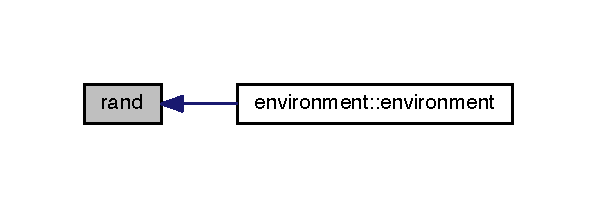
\includegraphics[width=286pt]{a00112_a078f67f8fbdd9ac6587e03bdf2651d32_icgraph}
\end{center}
\end{figure}


\hypertarget{a00112_acd685f63a27f53fc049aff633634ddd6}{\index{lancia\+\_\+inizializzatore\+\_\+acs.\+m@{lancia\+\_\+inizializzatore\+\_\+acs.\+m}!ratio\+\_\+firing\+\_\+disk@{ratio\+\_\+firing\+\_\+disk}}
\index{ratio\+\_\+firing\+\_\+disk@{ratio\+\_\+firing\+\_\+disk}!lancia\+\_\+inizializzatore\+\_\+acs.\+m@{lancia\+\_\+inizializzatore\+\_\+acs.\+m}}
\subsubsection[{ratio\+\_\+firing\+\_\+disk}]{\setlength{\rightskip}{0pt plus 5cm}id ratio\+\_\+firing\+\_\+disk (
\begin{DoxyParamCaption}
{}
\end{DoxyParamCaption}
)\hspace{0.3cm}{\ttfamily [virtual]}}}\label{a00112_acd685f63a27f53fc049aff633634ddd6}


\subsection{Variable Documentation}
\hypertarget{a00112_af03d45d99b8b6004fff00fbca936a3ce}{\index{lancia\+\_\+inizializzatore\+\_\+acs.\+m@{lancia\+\_\+inizializzatore\+\_\+acs.\+m}!\+\_\+\+\_\+pad0\+\_\+\+\_\+@{\+\_\+\+\_\+pad0\+\_\+\+\_\+}}
\index{\+\_\+\+\_\+pad0\+\_\+\+\_\+@{\+\_\+\+\_\+pad0\+\_\+\+\_\+}!lancia\+\_\+inizializzatore\+\_\+acs.\+m@{lancia\+\_\+inizializzatore\+\_\+acs.\+m}}
\subsubsection[{\+\_\+\+\_\+pad0\+\_\+\+\_\+}]{\setlength{\rightskip}{0pt plus 5cm}experiment \+\_\+\+\_\+pad0\+\_\+\+\_\+}}\label{a00112_af03d45d99b8b6004fff00fbca936a3ce}


Definition at line 27 of file lancia\+\_\+inizializzatore\+\_\+acs.\+m.

\hypertarget{a00112_a6ea019326f9d9d9c5e10160c5c4b6679}{\index{lancia\+\_\+inizializzatore\+\_\+acs.\+m@{lancia\+\_\+inizializzatore\+\_\+acs.\+m}!\+\_\+\+\_\+pad1\+\_\+\+\_\+@{\+\_\+\+\_\+pad1\+\_\+\+\_\+}}
\index{\+\_\+\+\_\+pad1\+\_\+\+\_\+@{\+\_\+\+\_\+pad1\+\_\+\+\_\+}!lancia\+\_\+inizializzatore\+\_\+acs.\+m@{lancia\+\_\+inizializzatore\+\_\+acs.\+m}}
\subsubsection[{\+\_\+\+\_\+pad1\+\_\+\+\_\+}]{\setlength{\rightskip}{0pt plus 5cm}experiment \+\_\+\+\_\+pad1\+\_\+\+\_\+}}\label{a00112_a6ea019326f9d9d9c5e10160c5c4b6679}


Definition at line 45 of file lancia\+\_\+inizializzatore\+\_\+acs.\+m.

\hypertarget{a00112_a43895072f7337df80dc4273211c55c9b}{\index{lancia\+\_\+inizializzatore\+\_\+acs.\+m@{lancia\+\_\+inizializzatore\+\_\+acs.\+m}!\+\_\+\+\_\+pad2\+\_\+\+\_\+@{\+\_\+\+\_\+pad2\+\_\+\+\_\+}}
\index{\+\_\+\+\_\+pad2\+\_\+\+\_\+@{\+\_\+\+\_\+pad2\+\_\+\+\_\+}!lancia\+\_\+inizializzatore\+\_\+acs.\+m@{lancia\+\_\+inizializzatore\+\_\+acs.\+m}}
\subsubsection[{\+\_\+\+\_\+pad2\+\_\+\+\_\+}]{\setlength{\rightskip}{0pt plus 5cm}experiment \+\_\+\+\_\+pad2\+\_\+\+\_\+}}\label{a00112_a43895072f7337df80dc4273211c55c9b}


Definition at line 57 of file lancia\+\_\+inizializzatore\+\_\+acs.\+m.

\hypertarget{a00112_abcbc32fc68e4323620d6171a17310212}{\index{lancia\+\_\+inizializzatore\+\_\+acs.\+m@{lancia\+\_\+inizializzatore\+\_\+acs.\+m}!alphabet@{alphabet}}
\index{alphabet@{alphabet}!lancia\+\_\+inizializzatore\+\_\+acs.\+m@{lancia\+\_\+inizializzatore\+\_\+acs.\+m}}
\subsubsection[{alphabet}]{\setlength{\rightskip}{0pt plus 5cm}alphabet = \mbox{[}'{\bf A\+B}'\mbox{]}}}\label{a00112_abcbc32fc68e4323620d6171a17310212}


Definition at line 29 of file lancia\+\_\+inizializzatore\+\_\+acs.\+m.

\hypertarget{a00112_a089ff88e71c60b850d67fa1c891af4ab}{\index{lancia\+\_\+inizializzatore\+\_\+acs.\+m@{lancia\+\_\+inizializzatore\+\_\+acs.\+m}!catalizzatori@{catalizzatori}}
\index{catalizzatori@{catalizzatori}!lancia\+\_\+inizializzatore\+\_\+acs.\+m@{lancia\+\_\+inizializzatore\+\_\+acs.\+m}}
\subsubsection[{catalizzatori}]{\setlength{\rightskip}{0pt plus 5cm}esponente della powerlaw in caso parametri per la distribuzione dei catalizzatori}}\label{a00112_a089ff88e71c60b850d67fa1c891af4ab}


Definition at line 89 of file lancia\+\_\+inizializzatore\+\_\+acs.\+m.

\hypertarget{a00112_ad4d86c1b55f9f76727181b05251ab7b1}{\index{lancia\+\_\+inizializzatore\+\_\+acs.\+m@{lancia\+\_\+inizializzatore\+\_\+acs.\+m}!complex\+Formation\+Symmetry@{complex\+Formation\+Symmetry}}
\index{complex\+Formation\+Symmetry@{complex\+Formation\+Symmetry}!lancia\+\_\+inizializzatore\+\_\+acs.\+m@{lancia\+\_\+inizializzatore\+\_\+acs.\+m}}
\subsubsection[{complex\+Formation\+Symmetry}]{\setlength{\rightskip}{0pt plus 5cm}complex\+Formation\+Symmetry =0}}\label{a00112_ad4d86c1b55f9f76727181b05251ab7b1}


Definition at line 51 of file lancia\+\_\+inizializzatore\+\_\+acs.\+m.

\hypertarget{a00112_a9341167cb56ed18499df723220990b9c}{\index{lancia\+\_\+inizializzatore\+\_\+acs.\+m@{lancia\+\_\+inizializzatore\+\_\+acs.\+m}!diffusion\+\_\+contribute@{diffusion\+\_\+contribute}}
\index{diffusion\+\_\+contribute@{diffusion\+\_\+contribute}!lancia\+\_\+inizializzatore\+\_\+acs.\+m@{lancia\+\_\+inizializzatore\+\_\+acs.\+m}}
\subsubsection[{diffusion\+\_\+contribute}]{\setlength{\rightskip}{0pt plus 5cm}diffusion\+\_\+contribute =0}}\label{a00112_a9341167cb56ed18499df723220990b9c}


Definition at line 75 of file lancia\+\_\+inizializzatore\+\_\+acs.\+m.

\hypertarget{a00112_aa25e2dab413d379872aab3c4023d62f7}{\index{lancia\+\_\+inizializzatore\+\_\+acs.\+m@{lancia\+\_\+inizializzatore\+\_\+acs.\+m}!energy\+Target@{energy\+Target}}
\index{energy\+Target@{energy\+Target}!lancia\+\_\+inizializzatore\+\_\+acs.\+m@{lancia\+\_\+inizializzatore\+\_\+acs.\+m}}
\subsubsection[{energy\+Target}]{\setlength{\rightskip}{0pt plus 5cm}energy\+Target =0}}\label{a00112_aa25e2dab413d379872aab3c4023d62f7}


Definition at line 49 of file lancia\+\_\+inizializzatore\+\_\+acs.\+m.

\hypertarget{a00112_af142377b5a19c7c6cdeba9a34c579682}{\index{lancia\+\_\+inizializzatore\+\_\+acs.\+m@{lancia\+\_\+inizializzatore\+\_\+acs.\+m}!fino\+\_\+a\+\_\+che\+\_\+lunghezza\+\_\+i\+\_\+polimeri\+\_\+non\+\_\+catalizzano@{fino\+\_\+a\+\_\+che\+\_\+lunghezza\+\_\+i\+\_\+polimeri\+\_\+non\+\_\+catalizzano}}
\index{fino\+\_\+a\+\_\+che\+\_\+lunghezza\+\_\+i\+\_\+polimeri\+\_\+non\+\_\+catalizzano@{fino\+\_\+a\+\_\+che\+\_\+lunghezza\+\_\+i\+\_\+polimeri\+\_\+non\+\_\+catalizzano}!lancia\+\_\+inizializzatore\+\_\+acs.\+m@{lancia\+\_\+inizializzatore\+\_\+acs.\+m}}
\subsubsection[{fino\+\_\+a\+\_\+che\+\_\+lunghezza\+\_\+i\+\_\+polimeri\+\_\+non\+\_\+catalizzano}]{\setlength{\rightskip}{0pt plus 5cm}$\ast$$\ast$ N\+E\+W$\ast$$\ast$ fino\+\_\+a\+\_\+che\+\_\+lunghezza\+\_\+i\+\_\+polimeri\+\_\+non\+\_\+catalizzano = 2}}\label{a00112_af142377b5a19c7c6cdeba9a34c579682}


Definition at line 54 of file lancia\+\_\+inizializzatore\+\_\+acs.\+m.

\hypertarget{a00112_a778a1aec6ffefe5cf8721850b92e487b}{\index{lancia\+\_\+inizializzatore\+\_\+acs.\+m@{lancia\+\_\+inizializzatore\+\_\+acs.\+m}!fosforilazione@{fosforilazione}}
\index{fosforilazione@{fosforilazione}!lancia\+\_\+inizializzatore\+\_\+acs.\+m@{lancia\+\_\+inizializzatore\+\_\+acs.\+m}}
\subsubsection[{fosforilazione}]{\setlength{\rightskip}{0pt plus 5cm}coefficiente di fosforilazione}}\label{a00112_a778a1aec6ffefe5cf8721850b92e487b}


Definition at line 68 of file lancia\+\_\+inizializzatore\+\_\+acs.\+m.

\hypertarget{a00112_a7cd0915d7542523abc226a8eecf67ecf}{\index{lancia\+\_\+inizializzatore\+\_\+acs.\+m@{lancia\+\_\+inizializzatore\+\_\+acs.\+m}!gamma\+\_\+powerlaw\+\_\+concentrazioni@{gamma\+\_\+powerlaw\+\_\+concentrazioni}}
\index{gamma\+\_\+powerlaw\+\_\+concentrazioni@{gamma\+\_\+powerlaw\+\_\+concentrazioni}!lancia\+\_\+inizializzatore\+\_\+acs.\+m@{lancia\+\_\+inizializzatore\+\_\+acs.\+m}}
\subsubsection[{gamma\+\_\+powerlaw\+\_\+concentrazioni}]{\setlength{\rightskip}{0pt plus 5cm}parametro uniforme sulle powerlaw con esponente gamma gamma\+\_\+powerlaw\+\_\+concentrazioni = 2.\+1}}\label{a00112_a7cd0915d7542523abc226a8eecf67ecf}


Definition at line 85 of file lancia\+\_\+inizializzatore\+\_\+acs.\+m.

\hypertarget{a00112_a6f6ccfcf58b31cb6412107d9d5281426}{\index{lancia\+\_\+inizializzatore\+\_\+acs.\+m@{lancia\+\_\+inizializzatore\+\_\+acs.\+m}!i@{i}}
\index{i@{i}!lancia\+\_\+inizializzatore\+\_\+acs.\+m@{lancia\+\_\+inizializzatore\+\_\+acs.\+m}}
\subsubsection[{i}]{\setlength{\rightskip}{0pt plus 5cm}for i}}\label{a00112_a6f6ccfcf58b31cb6412107d9d5281426}
{\bfseries Initial value\+:}
\begin{DoxyCode}
= 1:\hyperlink{a00112_a04ee275ab8ce56c2c9c8b2b82995a9f7}{massima\_lunghezza\_su\_cui\_calcolare\_le\_reazioni}
    \hyperlink{a00112_ac9358e0c7555a21532187de31cdbd469}{lastFiringDiskSpeciesID} = \hyperlink{a00112_ac9358e0c7555a21532187de31cdbd469}{lastFiringDiskSpeciesID} + 
      length(\hyperlink{a00112_abcbc32fc68e4323620d6171a17310212}{alphabet})^\hyperlink{a00112_a6f6ccfcf58b31cb6412107d9d5281426}{i}
\end{DoxyCode}


Definition at line 33 of file lancia\+\_\+inizializzatore\+\_\+acs.\+m.

\hypertarget{a00112_a637d2af7e7b03600bcaf1931b999e3fc}{\index{lancia\+\_\+inizializzatore\+\_\+acs.\+m@{lancia\+\_\+inizializzatore\+\_\+acs.\+m}!influx@{influx}}
\index{influx@{influx}!lancia\+\_\+inizializzatore\+\_\+acs.\+m@{lancia\+\_\+inizializzatore\+\_\+acs.\+m}}
\subsubsection[{influx}]{\setlength{\rightskip}{0pt plus 5cm}{\bf controllo} che non ci siano cicli nell influx =2}}\label{a00112_a637d2af7e7b03600bcaf1931b999e3fc}


Definition at line 77 of file lancia\+\_\+inizializzatore\+\_\+acs.\+m.

\hypertarget{a00112_ad795c71664f3161dc8f7a769341daadf}{\index{lancia\+\_\+inizializzatore\+\_\+acs.\+m@{lancia\+\_\+inizializzatore\+\_\+acs.\+m}!influx\+\_\+rate@{influx\+\_\+rate}}
\index{influx\+\_\+rate@{influx\+\_\+rate}!lancia\+\_\+inizializzatore\+\_\+acs.\+m@{lancia\+\_\+inizializzatore\+\_\+acs.\+m}}
\subsubsection[{influx\+\_\+rate}]{\setlength{\rightskip}{0pt plus 5cm}influx\+\_\+rate =1e-\/6}}\label{a00112_ad795c71664f3161dc8f7a769341daadf}


Definition at line 78 of file lancia\+\_\+inizializzatore\+\_\+acs.\+m.

\hypertarget{a00112_a4c7433c24b6426a15069cc5a93a5cbec}{\index{lancia\+\_\+inizializzatore\+\_\+acs.\+m@{lancia\+\_\+inizializzatore\+\_\+acs.\+m}!initial\+Max\+Length@{initial\+Max\+Length}}
\index{initial\+Max\+Length@{initial\+Max\+Length}!lancia\+\_\+inizializzatore\+\_\+acs.\+m@{lancia\+\_\+inizializzatore\+\_\+acs.\+m}}
\subsubsection[{initial\+Max\+Length}]{\setlength{\rightskip}{0pt plus 5cm}initial\+Max\+Length =3}}\label{a00112_a4c7433c24b6426a15069cc5a93a5cbec}


Definition at line 23 of file lancia\+\_\+inizializzatore\+\_\+acs.\+m.

\hypertarget{a00112_ae44c52e8cc45368288e687e5c374764f}{\index{lancia\+\_\+inizializzatore\+\_\+acs.\+m@{lancia\+\_\+inizializzatore\+\_\+acs.\+m}!initial\+Population\+Number@{initial\+Population\+Number}}
\index{initial\+Population\+Number@{initial\+Population\+Number}!lancia\+\_\+inizializzatore\+\_\+acs.\+m@{lancia\+\_\+inizializzatore\+\_\+acs.\+m}}
\subsubsection[{initial\+Population\+Number}]{\setlength{\rightskip}{0pt plus 5cm}initial\+Population\+Number =0}}\label{a00112_ae44c52e8cc45368288e687e5c374764f}


Definition at line 21 of file lancia\+\_\+inizializzatore\+\_\+acs.\+m.

\hypertarget{a00112_ada2b06fc2d132c7a047984505d3bad7c}{\index{lancia\+\_\+inizializzatore\+\_\+acs.\+m@{lancia\+\_\+inizializzatore\+\_\+acs.\+m}!inizializzatore\+\_\+\+A\+C\+S@{inizializzatore\+\_\+\+A\+C\+S}}
\index{inizializzatore\+\_\+\+A\+C\+S@{inizializzatore\+\_\+\+A\+C\+S}!lancia\+\_\+inizializzatore\+\_\+acs.\+m@{lancia\+\_\+inizializzatore\+\_\+acs.\+m}}
\subsubsection[{inizializzatore\+\_\+\+A\+C\+S}]{\setlength{\rightskip}{0pt plus 5cm}richiamo la funzione inizializzatore\+\_\+\+A\+C\+S\mbox{[}fd concentrazioni {\bf specie\+\_\+def} {\bf influx} {\bf catalizzatore} {\bf reazione} {\bf specie\+\_\+non\+\_\+esistenti} {\bf matrice\+\_\+adiacenza\+\_\+sub\+\_\+prod} {\bf matrice\+\_\+adiacenza\+\_\+cat\+\_\+prod}\mbox{]} = inizializzatore\+\_\+\+A\+C\+S({\bf n\+G\+E\+N}, {\bf n\+S\+I\+M}, {\bf n\+Seconds}, {\bf n\+Reactions}, {\bf initial\+Population\+Number}, {\bf initial\+Max\+Length}, {\bf massima\+\_\+lunghezza\+\_\+su\+\_\+cui\+\_\+calcolare\+\_\+le\+\_\+reazioni}, {\bf overall\+Concentration}, {\bf alphabet}, {\bf complex\+Formation\+Symmetry}, {\bf fino\+\_\+a\+\_\+che\+\_\+lunghezza\+\_\+i\+\_\+polimeri\+\_\+non\+\_\+catalizzano}, {\bf reaction\+Probability}, {\bf cleavage\+Probability}, {\bf diffusion\+\_\+contribute}, {\bf solubility\+\_\+threshold}, {\bf influx}, {\bf influx\+\_\+rate}, {\bf reverse\+Reactions}, {\bf Kass\+\_\+o\+\_\+\+Kdiss},{\bf rapporto\+\_\+\+Kfor\+\_\+\+Kback},rapporto\+\_\+\+Kcpx\+\_\+\+K\+\_\+ass,{\bf K\+\_\+cpx\+Diss}, {\bf K\+\_\+nrg}, {\bf molecule\+Decay\+\_\+\+Kinetic\+Constant}, {\bf ratio\+\_\+firing\+\_\+disk}, {\bf lunghezza\+\_\+max\+\_\+fd}, {\bf scelta\+\_\+concentrazioni}, {\bf gamma\+\_\+powerlaw\+\_\+concentrazioni},{\bf decisione\+\_\+catalizzatori}, {\bf last\+Firing\+Disk\+Species\+I\+D}, E\+C\+Concentration, {\bf volume}, {\bf energy}, {\bf energy\+Target}, controllo\+\_\+\+A\+C\+S\+\_\+nel\+\_\+ciclo, {\bf K\+\_\+irrad})}}\label{a00112_ada2b06fc2d132c7a047984505d3bad7c}


Definition at line 100 of file lancia\+\_\+inizializzatore\+\_\+acs.\+m.

\hypertarget{a00112_ab2422609d179c881c72aced926f83e6f}{\index{lancia\+\_\+inizializzatore\+\_\+acs.\+m@{lancia\+\_\+inizializzatore\+\_\+acs.\+m}!K\+\_\+cpx\+Diss@{K\+\_\+cpx\+Diss}}
\index{K\+\_\+cpx\+Diss@{K\+\_\+cpx\+Diss}!lancia\+\_\+inizializzatore\+\_\+acs.\+m@{lancia\+\_\+inizializzatore\+\_\+acs.\+m}}
\subsubsection[{K\+\_\+cpx\+Diss}]{\setlength{\rightskip}{0pt plus 5cm}K\+\_\+cpx\+Diss =0}}\label{a00112_ab2422609d179c881c72aced926f83e6f}


Definition at line 66 of file lancia\+\_\+inizializzatore\+\_\+acs.\+m.

\hypertarget{a00112_af915279099be3650c90bf0a3cf396e04}{\index{lancia\+\_\+inizializzatore\+\_\+acs.\+m@{lancia\+\_\+inizializzatore\+\_\+acs.\+m}!K\+\_\+eq@{K\+\_\+eq}}
\index{K\+\_\+eq@{K\+\_\+eq}!lancia\+\_\+inizializzatore\+\_\+acs.\+m@{lancia\+\_\+inizializzatore\+\_\+acs.\+m}}
\subsubsection[{K\+\_\+eq}]{\setlength{\rightskip}{0pt plus 5cm}costanti C\+I\+N\+E\+T\+I\+C\+H\+E K\+\_\+eq =1000}}\label{a00112_af915279099be3650c90bf0a3cf396e04}


Definition at line 61 of file lancia\+\_\+inizializzatore\+\_\+acs.\+m.

\hypertarget{a00112_abca6e303f83cae224170f5fd2f1fedfe}{\index{lancia\+\_\+inizializzatore\+\_\+acs.\+m@{lancia\+\_\+inizializzatore\+\_\+acs.\+m}!K\+\_\+irrad@{K\+\_\+irrad}}
\index{K\+\_\+irrad@{K\+\_\+irrad}!lancia\+\_\+inizializzatore\+\_\+acs.\+m@{lancia\+\_\+inizializzatore\+\_\+acs.\+m}}
\subsubsection[{K\+\_\+irrad}]{\setlength{\rightskip}{0pt plus 5cm}K\+\_\+irrad = 0}}\label{a00112_abca6e303f83cae224170f5fd2f1fedfe}


Definition at line 71 of file lancia\+\_\+inizializzatore\+\_\+acs.\+m.

\hypertarget{a00112_ac8f2b2a8d859ca2b7cf056575c7b0538}{\index{lancia\+\_\+inizializzatore\+\_\+acs.\+m@{lancia\+\_\+inizializzatore\+\_\+acs.\+m}!K\+\_\+nrg@{K\+\_\+nrg}}
\index{K\+\_\+nrg@{K\+\_\+nrg}!lancia\+\_\+inizializzatore\+\_\+acs.\+m@{lancia\+\_\+inizializzatore\+\_\+acs.\+m}}
\subsubsection[{K\+\_\+nrg}]{\setlength{\rightskip}{0pt plus 5cm}K\+\_\+nrg = 0}}\label{a00112_ac8f2b2a8d859ca2b7cf056575c7b0538}


Definition at line 69 of file lancia\+\_\+inizializzatore\+\_\+acs.\+m.

\hypertarget{a00112_a8d22b96a5ece64359002562ebc1fbfc5}{\index{lancia\+\_\+inizializzatore\+\_\+acs.\+m@{lancia\+\_\+inizializzatore\+\_\+acs.\+m}!kass@{kass}}
\index{kass@{kass}!lancia\+\_\+inizializzatore\+\_\+acs.\+m@{lancia\+\_\+inizializzatore\+\_\+acs.\+m}}
\subsubsection[{kass}]{\setlength{\rightskip}{0pt plus 5cm}{\bf se} � un cleavage {\bf se} � una condensazione kass =100}}\label{a00112_a8d22b96a5ece64359002562ebc1fbfc5}


Definition at line 63 of file lancia\+\_\+inizializzatore\+\_\+acs.\+m.

\hypertarget{a00112_a74947b8f8ce132902a228628db296032}{\index{lancia\+\_\+inizializzatore\+\_\+acs.\+m@{lancia\+\_\+inizializzatore\+\_\+acs.\+m}!Kass@{Kass}}
\index{Kass@{Kass}!lancia\+\_\+inizializzatore\+\_\+acs.\+m@{lancia\+\_\+inizializzatore\+\_\+acs.\+m}}
\subsubsection[{Kass}]{\setlength{\rightskip}{0pt plus 5cm}e g Kass}}\label{a00112_a74947b8f8ce132902a228628db296032}
{\bfseries Initial value\+:}
\begin{DoxyCode}
= 100 --> \hyperlink{a00113_a51a314f9df0eaa4488a1b264d1de0173}{Kdiss} = 100/100 = 1
rapporto\_Kcpx\_K\_ass = 0
\end{DoxyCode}


Definition at line 64 of file lancia\+\_\+inizializzatore\+\_\+acs.\+m.

\hypertarget{a00112_ace89973f1923711590b42efcf28a1f77}{\index{lancia\+\_\+inizializzatore\+\_\+acs.\+m@{lancia\+\_\+inizializzatore\+\_\+acs.\+m}!Kass\+\_\+o\+\_\+\+Kdiss@{Kass\+\_\+o\+\_\+\+Kdiss}}
\index{Kass\+\_\+o\+\_\+\+Kdiss@{Kass\+\_\+o\+\_\+\+Kdiss}!lancia\+\_\+inizializzatore\+\_\+acs.\+m@{lancia\+\_\+inizializzatore\+\_\+acs.\+m}}
\subsubsection[{Kass\+\_\+o\+\_\+\+Kdiss}]{\setlength{\rightskip}{0pt plus 5cm}parte da rivedere e correggere Kass\+\_\+o\+\_\+\+Kdiss = 0}}\label{a00112_ace89973f1923711590b42efcf28a1f77}


Definition at line 63 of file lancia\+\_\+inizializzatore\+\_\+acs.\+m.

\hypertarget{a00112_acb874616f80abe1a595c7c9e12040cd5}{\index{lancia\+\_\+inizializzatore\+\_\+acs.\+m@{lancia\+\_\+inizializzatore\+\_\+acs.\+m}!kdiss@{kdiss}}
\index{kdiss@{kdiss}!lancia\+\_\+inizializzatore\+\_\+acs.\+m@{lancia\+\_\+inizializzatore\+\_\+acs.\+m}}
\subsubsection[{kdiss}]{\setlength{\rightskip}{0pt plus 5cm}{\bf se} � un cleavage kdiss = 100}}\label{a00112_acb874616f80abe1a595c7c9e12040cd5}


Definition at line 63 of file lancia\+\_\+inizializzatore\+\_\+acs.\+m.

\hypertarget{a00112_ac9358e0c7555a21532187de31cdbd469}{\index{lancia\+\_\+inizializzatore\+\_\+acs.\+m@{lancia\+\_\+inizializzatore\+\_\+acs.\+m}!last\+Firing\+Disk\+Species\+I\+D@{last\+Firing\+Disk\+Species\+I\+D}}
\index{last\+Firing\+Disk\+Species\+I\+D@{last\+Firing\+Disk\+Species\+I\+D}!lancia\+\_\+inizializzatore\+\_\+acs.\+m@{lancia\+\_\+inizializzatore\+\_\+acs.\+m}}
\subsubsection[{last\+Firing\+Disk\+Species\+I\+D}]{\setlength{\rightskip}{0pt plus 5cm}{\bf end} last\+Firing\+Disk\+Species\+I\+D = 0}}\label{a00112_ac9358e0c7555a21532187de31cdbd469}


Definition at line 32 of file lancia\+\_\+inizializzatore\+\_\+acs.\+m.

\hypertarget{a00112_a7c974cc56015b6503e0619d32ebd4180}{\index{lancia\+\_\+inizializzatore\+\_\+acs.\+m@{lancia\+\_\+inizializzatore\+\_\+acs.\+m}!lunghezza\+\_\+max\+\_\+fd@{lunghezza\+\_\+max\+\_\+fd}}
\index{lunghezza\+\_\+max\+\_\+fd@{lunghezza\+\_\+max\+\_\+fd}!lancia\+\_\+inizializzatore\+\_\+acs.\+m@{lancia\+\_\+inizializzatore\+\_\+acs.\+m}}
\subsubsection[{lunghezza\+\_\+max\+\_\+fd}]{\setlength{\rightskip}{0pt plus 5cm}percentuale di specie da cancellare rispetto {\bf a} tutte quelle che restano dopo aver conservato {\bf i} polimeri fino {\bf a} lunghezzamaxfd lunghezza\+\_\+max\+\_\+fd = 1}}\label{a00112_a7c974cc56015b6503e0619d32ebd4180}


Definition at line 83 of file lancia\+\_\+inizializzatore\+\_\+acs.\+m.

\hypertarget{a00112_ad1bbbd24e4be6c7d8af30304c155c742}{\index{lancia\+\_\+inizializzatore\+\_\+acs.\+m@{lancia\+\_\+inizializzatore\+\_\+acs.\+m}!lunghezze@{lunghezze}}
\index{lunghezze@{lunghezze}!lancia\+\_\+inizializzatore\+\_\+acs.\+m@{lancia\+\_\+inizializzatore\+\_\+acs.\+m}}
\subsubsection[{lunghezze}]{\setlength{\rightskip}{0pt plus 5cm}parametro uniforme sulle lunghezze}}\label{a00112_ad1bbbd24e4be6c7d8af30304c155c742}


Definition at line 84 of file lancia\+\_\+inizializzatore\+\_\+acs.\+m.

\hypertarget{a00112_a04ee275ab8ce56c2c9c8b2b82995a9f7}{\index{lancia\+\_\+inizializzatore\+\_\+acs.\+m@{lancia\+\_\+inizializzatore\+\_\+acs.\+m}!massima\+\_\+lunghezza\+\_\+su\+\_\+cui\+\_\+calcolare\+\_\+le\+\_\+reazioni@{massima\+\_\+lunghezza\+\_\+su\+\_\+cui\+\_\+calcolare\+\_\+le\+\_\+reazioni}}
\index{massima\+\_\+lunghezza\+\_\+su\+\_\+cui\+\_\+calcolare\+\_\+le\+\_\+reazioni@{massima\+\_\+lunghezza\+\_\+su\+\_\+cui\+\_\+calcolare\+\_\+le\+\_\+reazioni}!lancia\+\_\+inizializzatore\+\_\+acs.\+m@{lancia\+\_\+inizializzatore\+\_\+acs.\+m}}
\subsubsection[{massima\+\_\+lunghezza\+\_\+su\+\_\+cui\+\_\+calcolare\+\_\+le\+\_\+reazioni}]{\setlength{\rightskip}{0pt plus 5cm}massima\+\_\+lunghezza\+\_\+su\+\_\+cui\+\_\+calcolare\+\_\+le\+\_\+reazioni = 3}}\label{a00112_a04ee275ab8ce56c2c9c8b2b82995a9f7}


Definition at line 24 of file lancia\+\_\+inizializzatore\+\_\+acs.\+m.

\hypertarget{a00112_aef2ea28de56b86a577b3c6fa0220926c}{\index{lancia\+\_\+inizializzatore\+\_\+acs.\+m@{lancia\+\_\+inizializzatore\+\_\+acs.\+m}!molecule\+Decay\+\_\+\+Kinetic\+Constant@{molecule\+Decay\+\_\+\+Kinetic\+Constant}}
\index{molecule\+Decay\+\_\+\+Kinetic\+Constant@{molecule\+Decay\+\_\+\+Kinetic\+Constant}!lancia\+\_\+inizializzatore\+\_\+acs.\+m@{lancia\+\_\+inizializzatore\+\_\+acs.\+m}}
\subsubsection[{molecule\+Decay\+\_\+\+Kinetic\+Constant}]{\setlength{\rightskip}{0pt plus 5cm}altri parametri molecule\+Decay\+\_\+\+Kinetic\+Constant =0.\+02}}\label{a00112_aef2ea28de56b86a577b3c6fa0220926c}


Definition at line 74 of file lancia\+\_\+inizializzatore\+\_\+acs.\+m.

\hypertarget{a00112_a7ab8b9fa18f22ee71429cf8ae50d754b}{\index{lancia\+\_\+inizializzatore\+\_\+acs.\+m@{lancia\+\_\+inizializzatore\+\_\+acs.\+m}!n\+Reactions@{n\+Reactions}}
\index{n\+Reactions@{n\+Reactions}!lancia\+\_\+inizializzatore\+\_\+acs.\+m@{lancia\+\_\+inizializzatore\+\_\+acs.\+m}}
\subsubsection[{n\+Reactions}]{\setlength{\rightskip}{0pt plus 5cm}n\+Reactions =200000000}}\label{a00112_a7ab8b9fa18f22ee71429cf8ae50d754b}


Definition at line 20 of file lancia\+\_\+inizializzatore\+\_\+acs.\+m.

\hypertarget{a00112_aaded2f2d61413dc4bddf805e9be03ded}{\index{lancia\+\_\+inizializzatore\+\_\+acs.\+m@{lancia\+\_\+inizializzatore\+\_\+acs.\+m}!n\+Seconds@{n\+Seconds}}
\index{n\+Seconds@{n\+Seconds}!lancia\+\_\+inizializzatore\+\_\+acs.\+m@{lancia\+\_\+inizializzatore\+\_\+acs.\+m}}
\subsubsection[{n\+Seconds}]{\setlength{\rightskip}{0pt plus 5cm}n\+Seconds =400}}\label{a00112_aaded2f2d61413dc4bddf805e9be03ded}


Definition at line 19 of file lancia\+\_\+inizializzatore\+\_\+acs.\+m.

\hypertarget{a00112_a68c8b36ce2387749248f566faa108e45}{\index{lancia\+\_\+inizializzatore\+\_\+acs.\+m@{lancia\+\_\+inizializzatore\+\_\+acs.\+m}!n\+S\+I\+M@{n\+S\+I\+M}}
\index{n\+S\+I\+M@{n\+S\+I\+M}!lancia\+\_\+inizializzatore\+\_\+acs.\+m@{lancia\+\_\+inizializzatore\+\_\+acs.\+m}}
\subsubsection[{n\+S\+I\+M}]{\setlength{\rightskip}{0pt plus 5cm}n\+S\+I\+M =1}}\label{a00112_a68c8b36ce2387749248f566faa108e45}


Definition at line 18 of file lancia\+\_\+inizializzatore\+\_\+acs.\+m.

\hypertarget{a00112_a59597688ed79473c0234f45eb9167574}{\index{lancia\+\_\+inizializzatore\+\_\+acs.\+m@{lancia\+\_\+inizializzatore\+\_\+acs.\+m}!overall\+Concentration@{overall\+Concentration}}
\index{overall\+Concentration@{overall\+Concentration}!lancia\+\_\+inizializzatore\+\_\+acs.\+m@{lancia\+\_\+inizializzatore\+\_\+acs.\+m}}
\subsubsection[{overall\+Concentration}]{\setlength{\rightskip}{0pt plus 5cm}overall\+Concentration =1e-\/4}}\label{a00112_a59597688ed79473c0234f45eb9167574}


Definition at line 38 of file lancia\+\_\+inizializzatore\+\_\+acs.\+m.

\hypertarget{a00112_acbcca8a3eb951a59ea95e6aa2be280fd}{\index{lancia\+\_\+inizializzatore\+\_\+acs.\+m@{lancia\+\_\+inizializzatore\+\_\+acs.\+m}!rapporto\+\_\+\+Kfor\+\_\+\+Kback@{rapporto\+\_\+\+Kfor\+\_\+\+Kback}}
\index{rapporto\+\_\+\+Kfor\+\_\+\+Kback@{rapporto\+\_\+\+Kfor\+\_\+\+Kback}!lancia\+\_\+inizializzatore\+\_\+acs.\+m@{lancia\+\_\+inizializzatore\+\_\+acs.\+m}}
\subsubsection[{rapporto\+\_\+\+Kfor\+\_\+\+Kback}]{\setlength{\rightskip}{0pt plus 5cm}rapporto\+\_\+\+Kfor\+\_\+\+Kback = 0}}\label{a00112_acbcca8a3eb951a59ea95e6aa2be280fd}


Definition at line 64 of file lancia\+\_\+inizializzatore\+\_\+acs.\+m.

\hypertarget{a00112_a9101beaeb03fddb5c6a9e68442177543}{\index{lancia\+\_\+inizializzatore\+\_\+acs.\+m@{lancia\+\_\+inizializzatore\+\_\+acs.\+m}!reaction\+Probability@{reaction\+Probability}}
\index{reaction\+Probability@{reaction\+Probability}!lancia\+\_\+inizializzatore\+\_\+acs.\+m@{lancia\+\_\+inizializzatore\+\_\+acs.\+m}}
\subsubsection[{reaction\+Probability}]{\setlength{\rightskip}{0pt plus 5cm}reaction\+Probability =0.\+004}}\label{a00112_a9101beaeb03fddb5c6a9e68442177543}


Definition at line 56 of file lancia\+\_\+inizializzatore\+\_\+acs.\+m.

\hypertarget{a00112_a650532b3a3c04865cc35cff6d567c5c0}{\index{lancia\+\_\+inizializzatore\+\_\+acs.\+m@{lancia\+\_\+inizializzatore\+\_\+acs.\+m}!reverse\+Reactions@{reverse\+Reactions}}
\index{reverse\+Reactions@{reverse\+Reactions}!lancia\+\_\+inizializzatore\+\_\+acs.\+m@{lancia\+\_\+inizializzatore\+\_\+acs.\+m}}
\subsubsection[{reverse\+Reactions}]{\setlength{\rightskip}{0pt plus 5cm}reverse\+Reactions =0}}\label{a00112_a650532b3a3c04865cc35cff6d567c5c0}


Definition at line 58 of file lancia\+\_\+inizializzatore\+\_\+acs.\+m.

\hypertarget{a00112_ac60b74a4c1b8bc23e64008ba1e0c41a8}{\index{lancia\+\_\+inizializzatore\+\_\+acs.\+m@{lancia\+\_\+inizializzatore\+\_\+acs.\+m}!scelta\+\_\+concentrazioni@{scelta\+\_\+concentrazioni}}
\index{scelta\+\_\+concentrazioni@{scelta\+\_\+concentrazioni}!lancia\+\_\+inizializzatore\+\_\+acs.\+m@{lancia\+\_\+inizializzatore\+\_\+acs.\+m}}
\subsubsection[{scelta\+\_\+concentrazioni}]{\setlength{\rightskip}{0pt plus 5cm}{\bf lunghezza} dei monomeri polimeri da conservare scelta\+\_\+concentrazioni =1}}\label{a00112_ac60b74a4c1b8bc23e64008ba1e0c41a8}


Definition at line 84 of file lancia\+\_\+inizializzatore\+\_\+acs.\+m.

\hypertarget{a00112_acbefa7c9bfd826fec9b32fa3bd29c288}{\index{lancia\+\_\+inizializzatore\+\_\+acs.\+m@{lancia\+\_\+inizializzatore\+\_\+acs.\+m}!solubility\+\_\+threshold@{solubility\+\_\+threshold}}
\index{solubility\+\_\+threshold@{solubility\+\_\+threshold}!lancia\+\_\+inizializzatore\+\_\+acs.\+m@{lancia\+\_\+inizializzatore\+\_\+acs.\+m}}
\subsubsection[{solubility\+\_\+threshold}]{\setlength{\rightskip}{0pt plus 5cm}solubility\+\_\+threshold =0}}\label{a00112_acbefa7c9bfd826fec9b32fa3bd29c288}


Definition at line 76 of file lancia\+\_\+inizializzatore\+\_\+acs.\+m.

\hypertarget{a00112_adc12f688ec66254762f4bdd2ce8c73df}{\index{lancia\+\_\+inizializzatore\+\_\+acs.\+m@{lancia\+\_\+inizializzatore\+\_\+acs.\+m}!switch@{switch}}
\index{switch@{switch}!lancia\+\_\+inizializzatore\+\_\+acs.\+m@{lancia\+\_\+inizializzatore\+\_\+acs.\+m}}
\subsubsection[{switch}]{\setlength{\rightskip}{0pt plus 5cm}parametro switch}}\label{a00112_adc12f688ec66254762f4bdd2ce8c73df}


Definition at line 84 of file lancia\+\_\+inizializzatore\+\_\+acs.\+m.

\hypertarget{a00112_a9bc498ccac8db41438f855f5dd3f4c05}{\index{lancia\+\_\+inizializzatore\+\_\+acs.\+m@{lancia\+\_\+inizializzatore\+\_\+acs.\+m}!volume@{volume}}
\index{volume@{volume}!lancia\+\_\+inizializzatore\+\_\+acs.\+m@{lancia\+\_\+inizializzatore\+\_\+acs.\+m}}
\subsubsection[{volume}]{\setlength{\rightskip}{0pt plus 5cm}volume =1e-\/15}}\label{a00112_a9bc498ccac8db41438f855f5dd3f4c05}


Definition at line 40 of file lancia\+\_\+inizializzatore\+\_\+acs.\+m.


\hypertarget{a00113}{\section{/\+Users/alessandrofilisetti/\+Documents/\+G\+I\+T/carness/\+\_\+matlabinitializator/start.m File Reference}
\label{a00113}\index{/\+Users/alessandrofilisetti/\+Documents/\+G\+I\+T/carness/\+\_\+matlabinitializator/start.\+m@{/\+Users/alessandrofilisetti/\+Documents/\+G\+I\+T/carness/\+\_\+matlabinitializator/start.\+m}}
}
\subsection*{Functions}
\begin{DoxyCompactItemize}
\item 
Numero di \hyperlink{a00113_a1b273eb41d82b5ca6c9f74a3c0aa2855}{simulazioni} (diversi semi random) \hyperlink{a00112_aaded2f2d61413dc4bddf805e9be03ded}{n\+Seconds}
\item 
Numero massimo di \hyperlink{a00113_a69962f56e60d0c88abc5d4b6839c2886}{reazioni} (secondo parametro di \hyperlink{a00030_a6bd08e37edf4151f5f6d1fc27a6f227a}{stop} oltre al numero di secondi) n\+Hours=0
\item 
Numero massimo di ore per la \hyperlink{a00113_ad4ff287bf077be8ffb479fcc197bc548}{simulazione} (=0 no vincolo) n\+Attempts=0
\item 
Numero di volte in cui sistema \\*
ritenta la stessa \hyperlink{a00113_a40d2922f55b48d94c99038a8c2bef2ff}{rete} (=0 no vincolo) \hyperlink{a00112_a4c7433c24b6426a15069cc5a93a5cbec}{initial\+Max\+Length}
\item 
Number of different networks \\*
for every network will be \\*
performed n\+Sim different \hyperlink{a00113_a096e1441156fd2c744baece86d6b295c}{simulation} (differnt random seeds) \hyperlink{a00027_abbf559a76fab59203496b0847ab9502a}{sim\+Folder.\+name}
\item 
\hyperlink{a00113_abe327856a9ee2f30f3ccafe4dc9edf5e}{cd} (\hyperlink{a00113_af28466084b87af2cdc5c7b48f4661f2d}{sim\+Folder.\+path}) \hyperlink{a00030_a01d55766b8058903dd360b4bda71f9f5}{if} \hyperlink{a00032_ab41b8dc78dee42a1a5e5a33d8bf6eeb3}{exist}(\hyperlink{a00027_abbf559a76fab59203496b0847ab9502a}{sim\+Folder.\+name}
\item 
converto in decimale for per \\*
default uniforme \hyperlink{a00113_aca80ac3e93dabd95e623a51f90fb37b6}{funzioni\+\_\+booleane\+\_\+in\+\_\+dec} (\hyperlink{a00113_ad3efca1ea6e3333daf30719ee0501862}{i}, 2)
\end{DoxyCompactItemize}
\subsection*{Variables}
\begin{DoxyCompactItemize}
\item 
lancia\+\_\+serie\+\_\+di\+\_\+inizializzatore \\*
m clear all close all \\*
$\ast$$\ast$$\ast$$\ast$$\ast$$\ast$$\ast$$\ast$$\ast$$\ast$$\ast$$\ast$$\ast$$\ast$$\ast$$\ast$$\ast$$\ast$$\ast$$\ast$$\ast$$\ast$$\ast$$\ast$$\ast$$\ast$$\ast$$\ast$$\ast$$\ast$$\ast$$\ast$$\ast$$\ast$$\ast$$\ast$$\ast$$\ast$$\ast$$\ast$$\ast$$\ast$$\ast$$\ast$$\ast$$\ast$$\ast$$\ast$$\ast$$\ast$$\ast$$\ast$$\ast$$\ast$$\ast$$\ast$$\ast$$\ast$$\ast$$\ast$$\ast$$\ast$$\ast$$\ast$$\ast$$\ast$$\ast$$\ast$$\ast$$\ast$$\ast$$\ast$$\ast$$\ast$Inserimento \\*
dei P\+A\+R\+A\+M\+E\+T\+R\+I V\+A\+R\+I\+A\+B\+I\+L\+I sui \\*
quali fare lo \hyperlink{a00113_abc4a849052f02bdfa554624d1d058817}{S\+C\+R\+E\+E\+N\+I\+N\+G}
\item 
lancia\+\_\+serie\+\_\+di\+\_\+inizializzatore \\*
m clear all close all \\*
$\ast$$\ast$$\ast$$\ast$$\ast$$\ast$$\ast$$\ast$$\ast$$\ast$$\ast$$\ast$$\ast$$\ast$$\ast$$\ast$$\ast$$\ast$$\ast$$\ast$$\ast$$\ast$$\ast$$\ast$$\ast$$\ast$$\ast$$\ast$$\ast$$\ast$$\ast$$\ast$$\ast$$\ast$$\ast$$\ast$$\ast$$\ast$$\ast$$\ast$$\ast$$\ast$$\ast$$\ast$$\ast$$\ast$$\ast$$\ast$$\ast$$\ast$$\ast$$\ast$$\ast$$\ast$$\ast$$\ast$$\ast$$\ast$$\ast$$\ast$$\ast$$\ast$$\ast$$\ast$$\ast$$\ast$$\ast$$\ast$$\ast$$\ast$$\ast$$\ast$$\ast$$\ast$Inserimento \\*
dei P\+A\+R\+A\+M\+E\+T\+R\+I V\+A\+R\+I\+A\+B\+I\+L\+I sui \\*
quali fare lo sottoforma di \\*
matrici o vettori \hyperlink{a00113_a9101beaeb03fddb5c6a9e68442177543}{reaction\+Probability} = \mbox{[}0.\+000516529
\item 
\hyperlink{a00113_ab05ea37ca64abe64c55c1f166e3a818b}{nome\+\_\+prob} = \mbox{[}0.\+125
\item 
\hyperlink{a00113_a2935a4c4576291c52f0dd2eb070e55e0}{l\+Max\+Influx} = \mbox{[}2\mbox{]}
\item 
\hyperlink{a00113_adc8f9d08ccff64cc5892dfd1791e14bc}{parametro\+\_\+screening} = \hyperlink{a00113_a2935a4c4576291c52f0dd2eb070e55e0}{l\+Max\+Influx}
\item 
\hyperlink{a00113_a277bc625a7a558f74ccc1eb2963d70d0}{nome\+\_\+folder} = \mbox{[}2\mbox{]}
\item 
$\ast$$\ast$$\ast$$\ast$$\ast$$\ast$$\ast$$\ast$$\ast$$\ast$$\ast$$\ast$$\ast$$\ast$$\ast$$\ast$$\ast$$\ast$$\ast$$\ast$$\ast$$\ast$$\ast$$\ast$$\ast$$\ast$$\ast$$\ast$$\ast$$\ast$$\ast$$\ast$$\ast$$\ast$$\ast$$\ast$$\ast$$\ast$$\ast$$\ast$$\ast$$\ast$$\ast$$\ast$$\ast$$\ast$$\ast$$\ast$$\ast$$\ast$$\ast$$\ast$$\ast$$\ast$$\ast$$\ast$$\ast$$\ast$$\ast$$\ast$$\ast$$\ast$$\ast$$\ast$$\ast$$\ast$$\ast$$\ast$$\ast$$\ast$$\ast$$\ast$$\ast$$\ast$$\ast$$\ast$$\ast$$\ast$$\ast$$\ast$$\ast$$\ast$$\ast$$\ast$$\ast$$\ast$$\ast$$\ast$$\ast$$\ast$$\ast$$\ast$$\ast$$\ast$$\ast$$\ast$$\ast$$\ast$$\ast$$\ast$$\ast$$\ast$$\ast$$\ast$$\ast$$\ast$$\ast$$\ast$$\ast$$\ast$$\ast$$\ast$$\ast$$\ast$$\ast$$\ast$$\ast$$\ast$$\ast$$\ast$$\ast$$\ast$$\ast$$\ast$$\ast$$\ast$$\ast$$\ast$$\ast$$\ast$$\ast$$\ast$$\ast$$\ast$$\ast$$\ast$$\ast$$\ast$$\ast$$\ast$$\ast$$\ast$$\ast$$\ast$$\ast$$\ast$$\ast$$\ast$Inserimento \\*
dei P\+A\+R\+A\+M\+E\+T\+R\+I \hyperlink{a00113_aea8a3181c0f6f0f47e51930921720484}{F\+I\+S\+S\+I}
\item 
$\ast$$\ast$$\ast$$\ast$$\ast$$\ast$$\ast$$\ast$$\ast$$\ast$$\ast$$\ast$$\ast$$\ast$$\ast$$\ast$$\ast$$\ast$$\ast$$\ast$$\ast$$\ast$$\ast$$\ast$$\ast$$\ast$$\ast$$\ast$$\ast$$\ast$$\ast$$\ast$$\ast$$\ast$$\ast$$\ast$$\ast$$\ast$$\ast$$\ast$$\ast$$\ast$$\ast$$\ast$$\ast$$\ast$$\ast$$\ast$$\ast$$\ast$$\ast$$\ast$$\ast$$\ast$$\ast$$\ast$$\ast$$\ast$$\ast$$\ast$$\ast$$\ast$$\ast$$\ast$$\ast$$\ast$$\ast$$\ast$$\ast$$\ast$$\ast$$\ast$$\ast$$\ast$$\ast$$\ast$$\ast$$\ast$$\ast$$\ast$$\ast$$\ast$$\ast$$\ast$$\ast$$\ast$$\ast$$\ast$$\ast$$\ast$$\ast$$\ast$$\ast$$\ast$$\ast$$\ast$$\ast$$\ast$$\ast$$\ast$$\ast$$\ast$$\ast$$\ast$$\ast$$\ast$$\ast$$\ast$$\ast$$\ast$$\ast$$\ast$$\ast$$\ast$$\ast$$\ast$$\ast$$\ast$$\ast$$\ast$$\ast$$\ast$$\ast$$\ast$$\ast$$\ast$$\ast$$\ast$$\ast$$\ast$$\ast$$\ast$$\ast$$\ast$$\ast$$\ast$$\ast$$\ast$$\ast$$\ast$$\ast$$\ast$$\ast$$\ast$$\ast$$\ast$$\ast$$\ast$Inserimento \\*
dei P\+A\+R\+A\+M\+E\+T\+R\+I quelli che \\*
restano cio costanti in tutti \\*
gli esperimenti della serie \hyperlink{a00113_adb2acbd590bcb59c7b4e633c250f3f28}{n\+S\+I\+M} =1
\item 
Numero di secondi \hyperlink{a00113_a422f03a95f0b273407ed13891d8d9f4d}{random\+Seed} =0
\item 
lasciare \hyperlink{a00035_a2ffdbad9ea59541e59cbd2b938e0770c}{a} \hyperlink{a00113_a08ef28bc85447e904ca9ea64de89b676}{debug\+Level} =0
\item 
livello di dettaglio messaggi \\*
durante \hyperlink{a00113_a31ca4d05639b265fc794a2776aa8fad3}{simulazione}
\item 
livello di dettaglio messaggi \\*
durante lasciare \hyperlink{a00113_a683f8d65c21f968751716fc09c13473b}{a}
\item 
livello di dettaglio messaggi \\*
durante lasciare per debug \\*
software \hyperlink{a00113_ae912a42ee691e9c69e17d5d791e0c71b}{time\+Structures\+Saving\+Interval} =\hyperlink{a00112_aaded2f2d61413dc4bddf805e9be03ded}{n\+Seconds}/100
\item 
definisce il tempo in cui \\*
vengono salvati \hyperlink{a00113_ad3efca1ea6e3333daf30719ee0501862}{i} \hyperlink{a00110_a4e8353d6c62cf54bf4a1a8f63e56b8c3}{file} durante \\*
la \hyperlink{a00113_ad4ff287bf077be8ffb479fcc197bc548}{simulazione} \hyperlink{a00113_a825ee95e200498001c9f82b9637c1ff5}{file\+Times\+Save\+Interval} =0
\item 
Definisce il tempo in cui \\*
vengono salvati \hyperlink{a00113_ad3efca1ea6e3333daf30719ee0501862}{i} dati sui \\*
\hyperlink{a00110_a4e8353d6c62cf54bf4a1a8f63e56b8c3}{file} \hyperlink{a00113_af3b4ff50e3fefed842dc431f3d32ff0e}{times}
\item 
Definisce il tempo in cui \\*
vengono salvati \hyperlink{a00113_ad3efca1ea6e3333daf30719ee0501862}{i} dati sui \\*
\hyperlink{a00110_a4e8353d6c62cf54bf4a1a8f63e56b8c3}{file} reaction\+\_\+parameter e \hyperlink{a00113_ad3efca1ea6e3333daf30719ee0501862}{i} \\*
vari living \hyperlink{a00113_a8d704532b4b419f1428cb078bb5c7ffe}{n\+Reactions} =200000000
\item 
Lunghezza massima delle specie \\*
da creare \hyperlink{a00113_a4e714d8e6551275aafab501b8c9f18ad}{massima\+\_\+lunghezza\+\_\+su\+\_\+cui\+\_\+calcolare\+\_\+le\+\_\+reazioni} = 6
\item 
Lunghezza massima fino alla \\*
quale creare le \hyperlink{a00113_a69962f56e60d0c88abc5d4b6839c2886}{reazioni} \hyperlink{a00113_abb126c97fed10420e64f85923bf5e04b}{max\+L\+Out} = 2
\item 
\hyperlink{a00113_a99032f27eaf45da350b544c68aa6467c}{se} =0 non viene considerato
\item 
altrimenti Quando \hyperlink{a00113_ad795c71664f3161dc8f7a769341daadf}{influx\+\_\+rate} \\*
indica la \hyperlink{a00106_a984d293145d85a936f430c0990316e51}{lunghezza} massima \\*
delle molecole che possono \\*
uscire dal \hyperlink{a00113_a8fcf98921930aa3720acdd081c5b0c2f}{contenitore}
\item 
altrimenti Quando influx\+\_\+rate \\*
indica la \hyperlink{a00106_a984d293145d85a936f430c0990316e51}{lunghezza} massima \\*
delle molecole che possono \\*
uscire dal quando \hyperlink{a00113_ad795c71664f3161dc8f7a769341daadf}{influx\+\_\+rate}
\item 
\hyperlink{a00113_abcbc32fc68e4323620d6171a17310212}{alphabet} = \mbox{[}'\hyperlink{a00111_abfef5bcdab19147dbfbb68112da17044}{A\+B}'\mbox{]}
\item 
\hyperlink{a00113_a59597688ed79473c0234f45eb9167574}{overall\+Concentration} =0.\+0333
\item 
\hyperlink{a00113_a9bc498ccac8db41438f855f5dd3f4c05}{volume} =1e-\/18
\item 
\hyperlink{a00113_ac002779c383d2cc783e881f94449de66}{energy} =0
\item 
energia \hyperlink{a00113_ad76697f83c5d8bf201c45822af227e21}{considerata}
\item 
energia non \hyperlink{a00113_ad76697f83c5d8bf201c45822af227e21}{considerata} \hyperlink{a00113_ac5d9cfec5453da5efc3e8d574b455833}{complex\+Formation\+Symmetry} =0
\item 
\hyperlink{a00113_ab6966d9ee620bc7376dc41a38352b948}{fino\+\_\+a\+\_\+che\+\_\+lunghezza\+\_\+i\+\_\+polimeri\+\_\+non\+\_\+catalizzano} = 2
\item 
\hyperlink{a00113_a9d512df05ee559766d2b8f08e4704b04}{cleavage\+Probability} =0.\+5
\item 
\hyperlink{a00113_a650532b3a3c04865cc35cff6d567c5c0}{reverse\+Reactions} =0
\item 
\hyperlink{a00113_a484afe97369bc993daaa71613dd2a665}{Kass} = 50
\item 
\hyperlink{a00113_a51a314f9df0eaa4488a1b264d1de0173}{Kdiss} = 25
\item 
\hyperlink{a00113_aaea32371e0f1645dcea44ce4d4a3d147}{Kcpx} = 50
\item 
\hyperlink{a00113_a26dbdfeb290332837753db666ee56981}{K\+\_\+cpx} = 1
\item 
\hyperlink{a00113_ac8f2b2a8d859ca2b7cf056575c7b0538}{K\+\_\+nrg} = 0
\item 
\hyperlink{a00113_abd02c282e86e2173abc6daed03f73584}{K\+\_\+nrg\+\_\+decay} =0
\item 
coefficiente di decadimento \\*
delle molecole o dei carrier \\*
dalla propria componente \\*
energetica \hyperlink{a00113_aa7d97d27bd1a172a2f0ad49ef13ef8ac}{rev\+Rct\+Ratio} = 10
\item 
\hyperlink{a00113_a1fa680d8b3a4f885d99f56fef41d2c37}{ratio\+Species\+Energizable} = 0
\item 
percentuale di specie presenti \\*
nel sistema che possono essere \\*
energizzate per ogni specie \\*
create \hyperlink{a00035_a6be92348ba85ef257b11d06209e1d7b6}{c} una certa probabilit \\*
di essere energizzabile o meno \hyperlink{a00113_a85569bbcfd8fbc0081b5a144eaf516f5}{molecule\+Decay\+\_\+\+Kinetic\+Constant} =0.\+02
\item 
\hyperlink{a00113_a9341167cb56ed18499df723220990b9c}{diffusion\+\_\+contribute} =0
\item 
\hyperlink{a00113_acbefa7c9bfd826fec9b32fa3bd29c288}{solubility\+\_\+threshold} =0
\item 
\hyperlink{a00106_a984d293145d85a936f430c0990316e51}{lunghezza} massima delle \\*
molecole presenti nell \hyperlink{a00107_a902e747aeec6b345d3a057099152f41f}{influx} \hyperlink{a00113_a83c1660d71068ae836121af0890bb3dd}{ratio\+\_\+firing\+\_\+disk} =0
\item 
percentuale di specie da \\*
cancellare rispetto \hyperlink{a00035_a2ffdbad9ea59541e59cbd2b938e0770c}{a} tutte \\*
quelle che restano dopo aver \\*
conservato \hyperlink{a00113_ad3efca1ea6e3333daf30719ee0501862}{i} polimeri fino \hyperlink{a00035_a2ffdbad9ea59541e59cbd2b938e0770c}{a} \\*
lunghezzamaxfd \hyperlink{a00113_a7c974cc56015b6503e0619d32ebd4180}{lunghezza\+\_\+max\+\_\+fd} = 7
\item 
\hyperlink{a00106_a984d293145d85a936f430c0990316e51}{lunghezza} dei monomeri \\*
polimeri da conservare \hyperlink{a00113_ac60b74a4c1b8bc23e64008ba1e0c41a8}{scelta\+\_\+concentrazioni} =1
\item 
parametro \hyperlink{a00113_adc12f688ec66254762f4bdd2ce8c73df}{switch}
\item 
parametro uniforme sulle \hyperlink{a00113_ad1bbbd24e4be6c7d8af30304c155c742}{lunghezze}
\item 
parametro uniforme sulle \\*
powerlaw con esponente gamma \hyperlink{a00113_a7cd0915d7542523abc226a8eecf67ecf}{gamma\+\_\+powerlaw\+\_\+concentrazioni} = 2.\+1
\item 
esponente della powerlaw in caso \hyperlink{a00113_a78948f867453293fcff0835b1bb05b8c}{decisione\+\_\+catalizzatori} =1
\item 
parametri per la distribuzione dei \hyperlink{a00113_a5a2da1d1b50e51c66813f40da0d9d0d1}{catalizzatori}
\item 
\hyperlink{a00110_adef1a44b5da0d8f5767284d2c6146569}{controllo} che non ci siano \\*
cicli nell \hyperlink{a00113_a637d2af7e7b03600bcaf1931b999e3fc}{influx}
\item 
N\+U\+O\+V\+O P\+A\+R\+A\+M\+E\+T\+R\+O \hyperlink{a00113_afd2d2a6a721b1dadfbf19213dbf732d8}{volume\+Growth} = 0
\item 
N\+U\+O\+V\+O P\+A\+R\+A\+M\+E\+T\+R\+O \hyperlink{a00113_a1c02ff40183f9cd6b495af789bb4ad05}{stoch\+Division} = 0
\item 
N\+U\+O\+V\+O P\+A\+R\+A\+M\+E\+T\+R\+O \hyperlink{a00032_aa671e3345005bd599e662bcaa115b18a}{sim\+Folder} \hyperlink{a00113_a006c95919fb4982bffba044f13cd2a7f}{nets} = 10
\item 
Number of different networks \hyperlink{a00113_a450b0c257ca2430779e4244700c076e7}{ensambles}
\item 
Nome della cartella dove verr \\*
salvata la \hyperlink{a00113_ad4ff287bf077be8ffb479fcc197bc548}{simulazione} \\*
\hyperlink{a00032_aa671e3345005bd599e662bcaa115b18a}{sim\+Folder} \hyperlink{a00113_af28466084b87af2cdc5c7b48f4661f2d}{path} = 'S\+I\+M\+S'
\item 
Percorso dove verr creata la \\*
cartella \hyperlink{a00032_aa671e3345005bd599e662bcaa115b18a}{sim\+Folder} dove \\*
verranno salvati tutti \hyperlink{a00113_ad3efca1ea6e3333daf30719ee0501862}{i} \hyperlink{a00110_a4e8353d6c62cf54bf4a1a8f63e56b8c3}{file} $\ast$$\ast$$\ast$$\ast$$\ast$$\ast$$\ast$$\ast$$\ast$$\ast$$\ast$$\ast$$\ast$$\ast$$\ast$$\ast$$\ast$$\ast$$\ast$$\ast$$\ast$$\ast$$\ast$$\ast$$\ast$$\ast$$\ast$$\ast$$\ast$$\ast$$\ast$$\ast$$\ast$$\ast$$\ast$$\ast$$\ast$$\ast$$\ast$$\ast$$\ast$$\ast$$\ast$$\ast$$\ast$$\ast$$\ast$$\ast$$\ast$$\ast$$\ast$$\ast$$\ast$$\ast$$\ast$$\ast$$\ast$$\ast$$\ast$$\ast$$\ast$$\ast$$\ast$$\ast$$\ast$$\ast$$\ast$$\ast$$\ast$$\ast$ \hyperlink{a00113_a4c8fe523edbe179c5d215da13f469f72}{n\+G\+E\+N} =10
\item 
Numero di \hyperlink{a00113_a5951b3462407a0e7e2e60534f76f5fec}{generazioni}
\item 
Numero di al momento significa \\*
che alla fine di ogni \\*
generazione da ogni \hyperlink{a00110_a4e8353d6c62cf54bf4a1a8f63e56b8c3}{file} di \\*
fine sim partono altre \hyperlink{a00113_af882a6050e97fe1c6cc2bb391ea57479}{Nsim}
\item 
Numero di al momento significa \\*
che alla fine di ogni \\*
generazione da ogni \hyperlink{a00110_a4e8353d6c62cf54bf4a1a8f63e56b8c3}{file} di \\*
fine sim partono altre \\*
lasciare ad \hyperlink{a00113_aafb51343927e7262fbd66ce291fdbb87}{!last\+Firing\+Disk\+Species\+I\+D} = 0
\item 
calcolata in automatico for \hyperlink{a00113_ad3efca1ea6e3333daf30719ee0501862}{i}
\item 
\hyperlink{a00025_afb358f48b1646c750fb9da6c6585be2b}{end} \hyperlink{a00113_ac9358e0c7555a21532187de31cdbd469}{last\+Firing\+Disk\+Species\+I\+D} = last\+Firing\+Disk\+Species\+I\+D -\/1
\item 
\hyperlink{a00113_a2d4125646b62462ce279d82913125ccf}{this\+Folder} = pwd
\item 
\hyperlink{a00113_a4ca269cf93df1b512b52174c1a256fe5}{dir}
\item 
\hyperlink{a00113_abe327856a9ee2f30f3ccafe4dc9edf5e}{cd}(\hyperlink{a00113_a2d4125646b62462ce279d82913125ccf}{this\+Folder})\%introduzione \\*
delle F\+U\+N\+Z\+I\+O\+N\+I B\+O\+O\+L\+E\+A\+N\+E nell'energia \hyperlink{a00113_af44cf9f59bd0c10b4d2aa541bd7c156b}{funzioni\+\_\+booleane\+\_\+in\+\_\+dec} = bi2de(funzioni\+\_\+booleane,'left-\/msb')
\item 
\hyperlink{a00113_a18f9e9dff2c5a2fe455a8d41fa6860fa}{parte2\+\_\+nome\+\_\+cartella} = num2str(\hyperlink{a00113_a277bc625a7a558f74ccc1eb2963d70d0}{nome\+\_\+folder}(\hyperlink{a00113_ad3efca1ea6e3333daf30719ee0501862}{i}))
\item 
\hyperlink{a00113_a1795e2dc228962c5b67eaee336bba2ad}{parte3\+\_\+nome\+\_\+cartella} = ('\+\_\+rete\+\_\+n\+\_\+')
\end{DoxyCompactItemize}


\subsection{Function Documentation}
\hypertarget{a00113_abe327856a9ee2f30f3ccafe4dc9edf5e}{\index{start.\+m@{start.\+m}!cd@{cd}}
\index{cd@{cd}!start.\+m@{start.\+m}}
\subsubsection[{cd}]{\setlength{\rightskip}{0pt plus 5cm}cd (
\begin{DoxyParamCaption}
\item[{sim\+Folder.}]{path}
\end{DoxyParamCaption}
)}}\label{a00113_abe327856a9ee2f30f3ccafe4dc9edf5e}
\hypertarget{a00113_aca80ac3e93dabd95e623a51f90fb37b6}{\index{start.\+m@{start.\+m}!funzioni\+\_\+booleane\+\_\+in\+\_\+dec@{funzioni\+\_\+booleane\+\_\+in\+\_\+dec}}
\index{funzioni\+\_\+booleane\+\_\+in\+\_\+dec@{funzioni\+\_\+booleane\+\_\+in\+\_\+dec}!start.\+m@{start.\+m}}
\subsubsection[{funzioni\+\_\+booleane\+\_\+in\+\_\+dec}]{\setlength{\rightskip}{0pt plus 5cm}converto in decimale for per default uniforme funzioni\+\_\+booleane\+\_\+in\+\_\+dec (
\begin{DoxyParamCaption}
\item[{{\bf i}}]{, }
\item[{2}]{}
\end{DoxyParamCaption}
)}}\label{a00113_aca80ac3e93dabd95e623a51f90fb37b6}
\hypertarget{a00113_a69962f56e60d0c88abc5d4b6839c2886}{\index{start.\+m@{start.\+m}!reazioni@{reazioni}}
\index{reazioni@{reazioni}!start.\+m@{start.\+m}}
\subsubsection[{reazioni}]{\setlength{\rightskip}{0pt plus 5cm}Numero massimo di reazioni (
\begin{DoxyParamCaption}
\item[{secondo parametro di {\bf stop} oltre al numero di}]{secondi}
\end{DoxyParamCaption}
)\hspace{0.3cm}{\ttfamily [pure virtual]}}}\label{a00113_a69962f56e60d0c88abc5d4b6839c2886}
\hypertarget{a00113_a40d2922f55b48d94c99038a8c2bef2ff}{\index{start.\+m@{start.\+m}!rete@{rete}}
\index{rete@{rete}!start.\+m@{start.\+m}}
\subsubsection[{rete}]{\setlength{\rightskip}{0pt plus 5cm}Numero di volte in cui sistema ritenta la stessa rete (
\begin{DoxyParamCaption}
{}
\end{DoxyParamCaption}
)}}\label{a00113_a40d2922f55b48d94c99038a8c2bef2ff}
\hypertarget{a00113_a096e1441156fd2c744baece86d6b295c}{\index{start.\+m@{start.\+m}!simulation@{simulation}}
\index{simulation@{simulation}!start.\+m@{start.\+m}}
\subsubsection[{simulation}]{\setlength{\rightskip}{0pt plus 5cm}Number of different networks for every network will be performed n\+Sim different simulation (
\begin{DoxyParamCaption}
\item[{differnt random}]{seeds}
\end{DoxyParamCaption}
)}}\label{a00113_a096e1441156fd2c744baece86d6b295c}
\hypertarget{a00113_ad4ff287bf077be8ffb479fcc197bc548}{\index{start.\+m@{start.\+m}!simulazione@{simulazione}}
\index{simulazione@{simulazione}!start.\+m@{start.\+m}}
\subsubsection[{simulazione}]{\setlength{\rightskip}{0pt plus 5cm}Numero massimo di ore per la simulazione (
\begin{DoxyParamCaption}
{}
\end{DoxyParamCaption}
)\hspace{0.3cm}{\ttfamily [pure virtual]}}}\label{a00113_ad4ff287bf077be8ffb479fcc197bc548}
\hypertarget{a00113_a1b273eb41d82b5ca6c9f74a3c0aa2855}{\index{start.\+m@{start.\+m}!simulazioni@{simulazioni}}
\index{simulazioni@{simulazioni}!start.\+m@{start.\+m}}
\subsubsection[{simulazioni}]{\setlength{\rightskip}{0pt plus 5cm}Numero di simulazioni (
\begin{DoxyParamCaption}
\item[{diversi semi}]{random}
\end{DoxyParamCaption}
)}}\label{a00113_a1b273eb41d82b5ca6c9f74a3c0aa2855}


\subsection{Variable Documentation}
\hypertarget{a00113_aafb51343927e7262fbd66ce291fdbb87}{\index{start.\+m@{start.\+m}!"!last\+Firing\+Disk\+Species\+I\+D@{"!last\+Firing\+Disk\+Species\+I\+D}}
\index{"!last\+Firing\+Disk\+Species\+I\+D@{"!last\+Firing\+Disk\+Species\+I\+D}!start.\+m@{start.\+m}}
\subsubsection[{"!last\+Firing\+Disk\+Species\+I\+D}]{\setlength{\rightskip}{0pt plus 5cm}Numero di al momento significa che alla fine di ogni generazione da ogni {\bf file} di fine sim partono altre lasciare ad !{\bf last\+Firing\+Disk\+Species\+I\+D} = 0}}\label{a00113_aafb51343927e7262fbd66ce291fdbb87}


Definition at line 79 of file start.\+m.

\hypertarget{a00113_a683f8d65c21f968751716fc09c13473b}{\index{start.\+m@{start.\+m}!a@{a}}
\index{a@{a}!start.\+m@{start.\+m}}
\subsubsection[{a}]{\setlength{\rightskip}{0pt plus 5cm}livello di dettaglio messaggi durante lasciare a}}\label{a00113_a683f8d65c21f968751716fc09c13473b}


Definition at line 26 of file start.\+m.

\hypertarget{a00113_abcbc32fc68e4323620d6171a17310212}{\index{start.\+m@{start.\+m}!alphabet@{alphabet}}
\index{alphabet@{alphabet}!start.\+m@{start.\+m}}
\subsubsection[{alphabet}]{\setlength{\rightskip}{0pt plus 5cm}alphabet = \mbox{[}'{\bf A\+B}'\mbox{]}}}\label{a00113_abcbc32fc68e4323620d6171a17310212}


Definition at line 36 of file start.\+m.

\hypertarget{a00113_a5a2da1d1b50e51c66813f40da0d9d0d1}{\index{start.\+m@{start.\+m}!catalizzatori@{catalizzatori}}
\index{catalizzatori@{catalizzatori}!start.\+m@{start.\+m}}
\subsubsection[{catalizzatori}]{\setlength{\rightskip}{0pt plus 5cm}parametri per la distribuzione dei catalizzatori}}\label{a00113_a5a2da1d1b50e51c66813f40da0d9d0d1}


Definition at line 63 of file start.\+m.

\hypertarget{a00113_a9d512df05ee559766d2b8f08e4704b04}{\index{start.\+m@{start.\+m}!cleavage\+Probability@{cleavage\+Probability}}
\index{cleavage\+Probability@{cleavage\+Probability}!start.\+m@{start.\+m}}
\subsubsection[{cleavage\+Probability}]{\setlength{\rightskip}{0pt plus 5cm}cleavage\+Probability =0.\+5}}\label{a00113_a9d512df05ee559766d2b8f08e4704b04}


Definition at line 42 of file start.\+m.

\hypertarget{a00113_ac5d9cfec5453da5efc3e8d574b455833}{\index{start.\+m@{start.\+m}!complex\+Formation\+Symmetry@{complex\+Formation\+Symmetry}}
\index{complex\+Formation\+Symmetry@{complex\+Formation\+Symmetry}!start.\+m@{start.\+m}}
\subsubsection[{complex\+Formation\+Symmetry}]{\setlength{\rightskip}{0pt plus 5cm}energia non {\bf considerata} complex\+Formation\+Symmetry =0}}\label{a00113_ac5d9cfec5453da5efc3e8d574b455833}


Definition at line 40 of file start.\+m.

\hypertarget{a00113_ad76697f83c5d8bf201c45822af227e21}{\index{start.\+m@{start.\+m}!considerata@{considerata}}
\index{considerata@{considerata}!start.\+m@{start.\+m}}
\subsubsection[{considerata}]{\setlength{\rightskip}{0pt plus 5cm}energia considerata}}\label{a00113_ad76697f83c5d8bf201c45822af227e21}


Definition at line 39 of file start.\+m.

\hypertarget{a00113_a8fcf98921930aa3720acdd081c5b0c2f}{\index{start.\+m@{start.\+m}!contenitore@{contenitore}}
\index{contenitore@{contenitore}!start.\+m@{start.\+m}}
\subsubsection[{contenitore}]{\setlength{\rightskip}{0pt plus 5cm}altrimenti Quando {\bf influx\+\_\+rate} indica la {\bf lunghezza} massima delle molecole che possono uscire dal contenitore}}\label{a00113_a8fcf98921930aa3720acdd081c5b0c2f}


Definition at line 34 of file start.\+m.

\hypertarget{a00113_a08ef28bc85447e904ca9ea64de89b676}{\index{start.\+m@{start.\+m}!debug\+Level@{debug\+Level}}
\index{debug\+Level@{debug\+Level}!start.\+m@{start.\+m}}
\subsubsection[{debug\+Level}]{\setlength{\rightskip}{0pt plus 5cm}lasciare {\bf a} debug\+Level =0}}\label{a00113_a08ef28bc85447e904ca9ea64de89b676}


Definition at line 26 of file start.\+m.

\hypertarget{a00113_a78948f867453293fcff0835b1bb05b8c}{\index{start.\+m@{start.\+m}!decisione\+\_\+catalizzatori@{decisione\+\_\+catalizzatori}}
\index{decisione\+\_\+catalizzatori@{decisione\+\_\+catalizzatori}!start.\+m@{start.\+m}}
\subsubsection[{decisione\+\_\+catalizzatori}]{\setlength{\rightskip}{0pt plus 5cm}esponente della powerlaw in caso decisione\+\_\+catalizzatori =1}}\label{a00113_a78948f867453293fcff0835b1bb05b8c}


Definition at line 62 of file start.\+m.

\hypertarget{a00113_a9341167cb56ed18499df723220990b9c}{\index{start.\+m@{start.\+m}!diffusion\+\_\+contribute@{diffusion\+\_\+contribute}}
\index{diffusion\+\_\+contribute@{diffusion\+\_\+contribute}!start.\+m@{start.\+m}}
\subsubsection[{diffusion\+\_\+contribute}]{\setlength{\rightskip}{0pt plus 5cm}diffusion\+\_\+contribute =0}}\label{a00113_a9341167cb56ed18499df723220990b9c}


Definition at line 54 of file start.\+m.

\hypertarget{a00113_a4ca269cf93df1b512b52174c1a256fe5}{\index{start.\+m@{start.\+m}!dir@{dir}}
\index{dir@{dir}!start.\+m@{start.\+m}}
\subsubsection[{dir}]{\setlength{\rightskip}{0pt plus 5cm}dir}}\label{a00113_a4ca269cf93df1b512b52174c1a256fe5}
{\bfseries Initial value\+:}
\begin{DoxyCode}
== 0
    \hyperlink{a00110_ae58a11ed5ac7873b1039a391d5c86a05}{mkdir}(\hyperlink{a00028_a0ffb8131632b48d9111c3a27d91262e2}{simFolder}.name)
\end{DoxyCode}


Definition at line 88 of file start.\+m.

\hypertarget{a00113_ac002779c383d2cc783e881f94449de66}{\index{start.\+m@{start.\+m}!energy@{energy}}
\index{energy@{energy}!start.\+m@{start.\+m}}
\subsubsection[{energy}]{\setlength{\rightskip}{0pt plus 5cm}energy =0}}\label{a00113_ac002779c383d2cc783e881f94449de66}


Definition at line 39 of file start.\+m.

\hypertarget{a00113_a450b0c257ca2430779e4244700c076e7}{\index{start.\+m@{start.\+m}!ensambles@{ensambles}}
\index{ensambles@{ensambles}!start.\+m@{start.\+m}}
\subsubsection[{ensambles}]{\setlength{\rightskip}{0pt plus 5cm}Number of different networks ensambles}}\label{a00113_a450b0c257ca2430779e4244700c076e7}


Definition at line 72 of file start.\+m.

\hypertarget{a00113_a825ee95e200498001c9f82b9637c1ff5}{\index{start.\+m@{start.\+m}!file\+Times\+Save\+Interval@{file\+Times\+Save\+Interval}}
\index{file\+Times\+Save\+Interval@{file\+Times\+Save\+Interval}!start.\+m@{start.\+m}}
\subsubsection[{file\+Times\+Save\+Interval}]{\setlength{\rightskip}{0pt plus 5cm}definisce il tempo in cui vengono salvati {\bf i} {\bf file} durante la {\bf simulazione} file\+Times\+Save\+Interval =0}}\label{a00113_a825ee95e200498001c9f82b9637c1ff5}


Definition at line 28 of file start.\+m.

\hypertarget{a00113_ab6966d9ee620bc7376dc41a38352b948}{\index{start.\+m@{start.\+m}!fino\+\_\+a\+\_\+che\+\_\+lunghezza\+\_\+i\+\_\+polimeri\+\_\+non\+\_\+catalizzano@{fino\+\_\+a\+\_\+che\+\_\+lunghezza\+\_\+i\+\_\+polimeri\+\_\+non\+\_\+catalizzano}}
\index{fino\+\_\+a\+\_\+che\+\_\+lunghezza\+\_\+i\+\_\+polimeri\+\_\+non\+\_\+catalizzano@{fino\+\_\+a\+\_\+che\+\_\+lunghezza\+\_\+i\+\_\+polimeri\+\_\+non\+\_\+catalizzano}!start.\+m@{start.\+m}}
\subsubsection[{fino\+\_\+a\+\_\+che\+\_\+lunghezza\+\_\+i\+\_\+polimeri\+\_\+non\+\_\+catalizzano}]{\setlength{\rightskip}{0pt plus 5cm}fino\+\_\+a\+\_\+che\+\_\+lunghezza\+\_\+i\+\_\+polimeri\+\_\+non\+\_\+catalizzano = 2}}\label{a00113_ab6966d9ee620bc7376dc41a38352b948}


Definition at line 41 of file start.\+m.

\hypertarget{a00113_aea8a3181c0f6f0f47e51930921720484}{\index{start.\+m@{start.\+m}!F\+I\+S\+S\+I@{F\+I\+S\+S\+I}}
\index{F\+I\+S\+S\+I@{F\+I\+S\+S\+I}!start.\+m@{start.\+m}}
\subsubsection[{F\+I\+S\+S\+I}]{\setlength{\rightskip}{0pt plus 5cm}$\ast$$\ast$$\ast$$\ast$$\ast$$\ast$$\ast$$\ast$$\ast$$\ast$$\ast$$\ast$$\ast$$\ast$$\ast$$\ast$$\ast$$\ast$$\ast$$\ast$$\ast$$\ast$$\ast$$\ast$$\ast$$\ast$$\ast$$\ast$$\ast$$\ast$$\ast$$\ast$$\ast$$\ast$$\ast$$\ast$$\ast$$\ast$$\ast$$\ast$$\ast$$\ast$$\ast$$\ast$$\ast$$\ast$$\ast$$\ast$$\ast$$\ast$$\ast$$\ast$$\ast$$\ast$$\ast$$\ast$$\ast$$\ast$$\ast$$\ast$$\ast$$\ast$$\ast$$\ast$$\ast$$\ast$$\ast$$\ast$$\ast$$\ast$$\ast$$\ast$$\ast$$\ast$ $\ast$$\ast$$\ast$$\ast$$\ast$$\ast$$\ast$$\ast$$\ast$$\ast$$\ast$$\ast$$\ast$$\ast$$\ast$$\ast$$\ast$$\ast$$\ast$$\ast$$\ast$$\ast$$\ast$$\ast$$\ast$$\ast$$\ast$$\ast$$\ast$$\ast$$\ast$$\ast$$\ast$$\ast$$\ast$$\ast$$\ast$$\ast$$\ast$$\ast$$\ast$$\ast$$\ast$$\ast$$\ast$$\ast$$\ast$$\ast$$\ast$$\ast$$\ast$$\ast$$\ast$$\ast$$\ast$$\ast$$\ast$$\ast$$\ast$$\ast$$\ast$$\ast$$\ast$$\ast$$\ast$$\ast$$\ast$$\ast$$\ast$$\ast$$\ast$$\ast$$\ast$$\ast$ Inserimento dei P\+A\+R\+A\+M\+E\+T\+R\+I F\+I\+S\+S\+I}}\label{a00113_aea8a3181c0f6f0f47e51930921720484}


Definition at line 20 of file start.\+m.

\hypertarget{a00113_af44cf9f59bd0c10b4d2aa541bd7c156b}{\index{start.\+m@{start.\+m}!funzioni\+\_\+booleane\+\_\+in\+\_\+dec@{funzioni\+\_\+booleane\+\_\+in\+\_\+dec}}
\index{funzioni\+\_\+booleane\+\_\+in\+\_\+dec@{funzioni\+\_\+booleane\+\_\+in\+\_\+dec}!start.\+m@{start.\+m}}
\subsubsection[{funzioni\+\_\+booleane\+\_\+in\+\_\+dec}]{\setlength{\rightskip}{0pt plus 5cm}converto in decimale funzioni\+\_\+booleane\+\_\+in\+\_\+dec = bi2de(funzioni\+\_\+booleane,'left-\/msb')}}\label{a00113_af44cf9f59bd0c10b4d2aa541bd7c156b}


Definition at line 119 of file start.\+m.

\hypertarget{a00113_a7cd0915d7542523abc226a8eecf67ecf}{\index{start.\+m@{start.\+m}!gamma\+\_\+powerlaw\+\_\+concentrazioni@{gamma\+\_\+powerlaw\+\_\+concentrazioni}}
\index{gamma\+\_\+powerlaw\+\_\+concentrazioni@{gamma\+\_\+powerlaw\+\_\+concentrazioni}!start.\+m@{start.\+m}}
\subsubsection[{gamma\+\_\+powerlaw\+\_\+concentrazioni}]{\setlength{\rightskip}{0pt plus 5cm}parametro uniforme sulle powerlaw con esponente gamma gamma\+\_\+powerlaw\+\_\+concentrazioni = 2.\+1}}\label{a00113_a7cd0915d7542523abc226a8eecf67ecf}


Definition at line 61 of file start.\+m.

\hypertarget{a00113_a5951b3462407a0e7e2e60534f76f5fec}{\index{start.\+m@{start.\+m}!generazioni@{generazioni}}
\index{generazioni@{generazioni}!start.\+m@{start.\+m}}
\subsubsection[{generazioni}]{\setlength{\rightskip}{0pt plus 5cm}Numero di generazioni}}\label{a00113_a5951b3462407a0e7e2e60534f76f5fec}


Definition at line 78 of file start.\+m.

\hypertarget{a00113_ad3efca1ea6e3333daf30719ee0501862}{\index{start.\+m@{start.\+m}!i@{i}}
\index{i@{i}!start.\+m@{start.\+m}}
\subsubsection[{i}]{\setlength{\rightskip}{0pt plus 5cm}{\bf end}$\ast$$\ast$$\ast$$\ast$$\ast$$\ast$$\ast$$\ast$$\ast$$\ast$$\ast$$\ast$$\ast$$\ast$$\ast$$\ast$$\ast$$\ast$$\ast$$\ast$$\ast$$\ast$$\ast$$\ast$$\ast$$\ast$$\ast$$\ast$$\ast$$\ast$$\ast$$\ast$$\ast$$\ast$$\ast$$\ast$$\ast$$\ast$$\ast$$\ast$$\ast$$\ast$$\ast$$\ast$$\ast$$\ast$$\ast$$\ast$$\ast$$\ast$$\ast$$\ast$$\ast$$\ast$$\ast$$\ast$$\ast$$\ast$$\ast$$\ast$$\ast$$\ast$$\ast$$\ast$$\ast$$\ast$$\ast$$\ast$$\ast$$\ast$$\ast$$\ast$$\ast$$\ast$ $\ast$$\ast$$\ast$$\ast$$\ast$$\ast$$\ast$$\ast$$\ast$$\ast$$\ast$$\ast$$\ast$$\ast$$\ast$$\ast$$\ast$$\ast$$\ast$$\ast$$\ast$ $\ast$$\ast$$\ast$$\ast$$\ast$ S T {\bf A} R T$\ast$$\ast$$\ast$$\ast$$\ast$ $\ast$$\ast$$\ast$$\ast$$\ast$$\ast$$\ast$$\ast$$\ast$$\ast$$\ast$$\ast$$\ast$$\ast$$\ast$$\ast$$\ast$$\ast$$\ast$$\ast$$\ast$ for i}}\label{a00113_ad3efca1ea6e3333daf30719ee0501862}
{\bfseries Initial value\+:}
\begin{DoxyCode}
= 1:\hyperlink{a00113_a4e714d8e6551275aafab501b8c9f18ad}{massima\_lunghezza\_su\_cui\_calcolare\_le\_reazioni}
    \hyperlink{a00113_ac9358e0c7555a21532187de31cdbd469}{lastFiringDiskSpeciesID} = \hyperlink{a00113_ac9358e0c7555a21532187de31cdbd469}{lastFiringDiskSpeciesID} + 
      length(\hyperlink{a00113_abcbc32fc68e4323620d6171a17310212}{alphabet})^\hyperlink{a00113_ad3efca1ea6e3333daf30719ee0501862}{i}
\end{DoxyCode}


Definition at line 80 of file start.\+m.

\hypertarget{a00113_a637d2af7e7b03600bcaf1931b999e3fc}{\index{start.\+m@{start.\+m}!influx@{influx}}
\index{influx@{influx}!start.\+m@{start.\+m}}
\subsubsection[{influx}]{\setlength{\rightskip}{0pt plus 5cm}{\bf controllo} che non ci siano cicli nell influx}}\label{a00113_a637d2af7e7b03600bcaf1931b999e3fc}


Definition at line 68 of file start.\+m.

\hypertarget{a00113_ad795c71664f3161dc8f7a769341daadf}{\index{start.\+m@{start.\+m}!influx\+\_\+rate@{influx\+\_\+rate}}
\index{influx\+\_\+rate@{influx\+\_\+rate}!start.\+m@{start.\+m}}
\subsubsection[{influx\+\_\+rate}]{\setlength{\rightskip}{0pt plus 5cm}influx\+\_\+rate}}\label{a00113_ad795c71664f3161dc8f7a769341daadf}
{\bfseries Initial value\+:}
\begin{DoxyCode}
= 0 indica fino \hyperlink{a00113_a683f8d65c21f968751716fc09c13473b}{a} quale \hyperlink{a00106_a984d293145d85a936f430c0990316e51}{lunghezza} le molecole non variano in quantita\textcolor{stringliteral}{' (simulazione membrana
       permeabile)}
\textcolor{stringliteral}{ECConcentration=0}
\end{DoxyCode}


Definition at line 34 of file start.\+m.

\hypertarget{a00113_a26dbdfeb290332837753db666ee56981}{\index{start.\+m@{start.\+m}!K\+\_\+cpx@{K\+\_\+cpx}}
\index{K\+\_\+cpx@{K\+\_\+cpx}!start.\+m@{start.\+m}}
\subsubsection[{K\+\_\+cpx}]{\setlength{\rightskip}{0pt plus 5cm}K\+\_\+cpx = 1}}\label{a00113_a26dbdfeb290332837753db666ee56981}


Definition at line 48 of file start.\+m.

\hypertarget{a00113_ac8f2b2a8d859ca2b7cf056575c7b0538}{\index{start.\+m@{start.\+m}!K\+\_\+nrg@{K\+\_\+nrg}}
\index{K\+\_\+nrg@{K\+\_\+nrg}!start.\+m@{start.\+m}}
\subsubsection[{K\+\_\+nrg}]{\setlength{\rightskip}{0pt plus 5cm}K\+\_\+nrg = 0}}\label{a00113_ac8f2b2a8d859ca2b7cf056575c7b0538}


Definition at line 49 of file start.\+m.

\hypertarget{a00113_abd02c282e86e2173abc6daed03f73584}{\index{start.\+m@{start.\+m}!K\+\_\+nrg\+\_\+decay@{K\+\_\+nrg\+\_\+decay}}
\index{K\+\_\+nrg\+\_\+decay@{K\+\_\+nrg\+\_\+decay}!start.\+m@{start.\+m}}
\subsubsection[{K\+\_\+nrg\+\_\+decay}]{\setlength{\rightskip}{0pt plus 5cm}K\+\_\+nrg\+\_\+decay =0}}\label{a00113_abd02c282e86e2173abc6daed03f73584}


Definition at line 50 of file start.\+m.

\hypertarget{a00113_a484afe97369bc993daaa71613dd2a665}{\index{start.\+m@{start.\+m}!Kass@{Kass}}
\index{Kass@{Kass}!start.\+m@{start.\+m}}
\subsubsection[{Kass}]{\setlength{\rightskip}{0pt plus 5cm}Kass = 50}}\label{a00113_a484afe97369bc993daaa71613dd2a665}


Definition at line 45 of file start.\+m.

\hypertarget{a00113_aaea32371e0f1645dcea44ce4d4a3d147}{\index{start.\+m@{start.\+m}!Kcpx@{Kcpx}}
\index{Kcpx@{Kcpx}!start.\+m@{start.\+m}}
\subsubsection[{Kcpx}]{\setlength{\rightskip}{0pt plus 5cm}Kcpx = 50}}\label{a00113_aaea32371e0f1645dcea44ce4d4a3d147}


Definition at line 47 of file start.\+m.

\hypertarget{a00113_a51a314f9df0eaa4488a1b264d1de0173}{\index{start.\+m@{start.\+m}!Kdiss@{Kdiss}}
\index{Kdiss@{Kdiss}!start.\+m@{start.\+m}}
\subsubsection[{Kdiss}]{\setlength{\rightskip}{0pt plus 5cm}Kdiss = 25}}\label{a00113_a51a314f9df0eaa4488a1b264d1de0173}


Definition at line 46 of file start.\+m.

\hypertarget{a00113_ac9358e0c7555a21532187de31cdbd469}{\index{start.\+m@{start.\+m}!last\+Firing\+Disk\+Species\+I\+D@{last\+Firing\+Disk\+Species\+I\+D}}
\index{last\+Firing\+Disk\+Species\+I\+D@{last\+Firing\+Disk\+Species\+I\+D}!start.\+m@{start.\+m}}
\subsubsection[{last\+Firing\+Disk\+Species\+I\+D}]{\setlength{\rightskip}{0pt plus 5cm}{\bf end} last\+Firing\+Disk\+Species\+I\+D = last\+Firing\+Disk\+Species\+I\+D -\/1}}\label{a00113_ac9358e0c7555a21532187de31cdbd469}


Definition at line 83 of file start.\+m.

\hypertarget{a00113_a2935a4c4576291c52f0dd2eb070e55e0}{\index{start.\+m@{start.\+m}!l\+Max\+Influx@{l\+Max\+Influx}}
\index{l\+Max\+Influx@{l\+Max\+Influx}!start.\+m@{start.\+m}}
\subsubsection[{l\+Max\+Influx}]{\setlength{\rightskip}{0pt plus 5cm}{\bf se} il sistema chiuso l\+Max\+Influx = \mbox{[}2\mbox{]}}}\label{a00113_a2935a4c4576291c52f0dd2eb070e55e0}


Definition at line 13 of file start.\+m.

\hypertarget{a00113_a7c974cc56015b6503e0619d32ebd4180}{\index{start.\+m@{start.\+m}!lunghezza\+\_\+max\+\_\+fd@{lunghezza\+\_\+max\+\_\+fd}}
\index{lunghezza\+\_\+max\+\_\+fd@{lunghezza\+\_\+max\+\_\+fd}!start.\+m@{start.\+m}}
\subsubsection[{lunghezza\+\_\+max\+\_\+fd}]{\setlength{\rightskip}{0pt plus 5cm}percentuale di specie da cancellare rispetto {\bf a} tutte quelle che restano dopo aver conservato {\bf i} polimeri fino {\bf a} lunghezzamaxfd lunghezza\+\_\+max\+\_\+fd = 7}}\label{a00113_a7c974cc56015b6503e0619d32ebd4180}


Definition at line 59 of file start.\+m.

\hypertarget{a00113_ad1bbbd24e4be6c7d8af30304c155c742}{\index{start.\+m@{start.\+m}!lunghezze@{lunghezze}}
\index{lunghezze@{lunghezze}!start.\+m@{start.\+m}}
\subsubsection[{lunghezze}]{\setlength{\rightskip}{0pt plus 5cm}parametro uniforme sulle lunghezze}}\label{a00113_ad1bbbd24e4be6c7d8af30304c155c742}


Definition at line 60 of file start.\+m.

\hypertarget{a00113_a4e714d8e6551275aafab501b8c9f18ad}{\index{start.\+m@{start.\+m}!massima\+\_\+lunghezza\+\_\+su\+\_\+cui\+\_\+calcolare\+\_\+le\+\_\+reazioni@{massima\+\_\+lunghezza\+\_\+su\+\_\+cui\+\_\+calcolare\+\_\+le\+\_\+reazioni}}
\index{massima\+\_\+lunghezza\+\_\+su\+\_\+cui\+\_\+calcolare\+\_\+le\+\_\+reazioni@{massima\+\_\+lunghezza\+\_\+su\+\_\+cui\+\_\+calcolare\+\_\+le\+\_\+reazioni}!start.\+m@{start.\+m}}
\subsubsection[{massima\+\_\+lunghezza\+\_\+su\+\_\+cui\+\_\+calcolare\+\_\+le\+\_\+reazioni}]{\setlength{\rightskip}{0pt plus 5cm}Lunghezza massima delle specie da creare massima\+\_\+lunghezza\+\_\+su\+\_\+cui\+\_\+calcolare\+\_\+le\+\_\+reazioni = 6}}\label{a00113_a4e714d8e6551275aafab501b8c9f18ad}


Definition at line 33 of file start.\+m.

\hypertarget{a00113_abb126c97fed10420e64f85923bf5e04b}{\index{start.\+m@{start.\+m}!max\+L\+Out@{max\+L\+Out}}
\index{max\+L\+Out@{max\+L\+Out}!start.\+m@{start.\+m}}
\subsubsection[{max\+L\+Out}]{\setlength{\rightskip}{0pt plus 5cm}Lunghezza massima fino alla quale creare le {\bf reazioni} max\+L\+Out = 2}}\label{a00113_abb126c97fed10420e64f85923bf5e04b}


Definition at line 34 of file start.\+m.

\hypertarget{a00113_a85569bbcfd8fbc0081b5a144eaf516f5}{\index{start.\+m@{start.\+m}!molecule\+Decay\+\_\+\+Kinetic\+Constant@{molecule\+Decay\+\_\+\+Kinetic\+Constant}}
\index{molecule\+Decay\+\_\+\+Kinetic\+Constant@{molecule\+Decay\+\_\+\+Kinetic\+Constant}!start.\+m@{start.\+m}}
\subsubsection[{molecule\+Decay\+\_\+\+Kinetic\+Constant}]{\setlength{\rightskip}{0pt plus 5cm}percentuale di specie presenti nel sistema che possono essere energizzate per ogni specie create {\bf c} una certa probabilit di essere energizzabile o meno molecule\+Decay\+\_\+\+Kinetic\+Constant =0.\+02}}\label{a00113_a85569bbcfd8fbc0081b5a144eaf516f5}


Definition at line 53 of file start.\+m.

\hypertarget{a00113_a006c95919fb4982bffba044f13cd2a7f}{\index{start.\+m@{start.\+m}!nets@{nets}}
\index{nets@{nets}!start.\+m@{start.\+m}}
\subsubsection[{nets}]{\setlength{\rightskip}{0pt plus 5cm}N\+U\+O\+V\+O P\+A\+R\+A\+M\+E\+T\+R\+O {\bf sim\+Folder} nets = 10}}\label{a00113_a006c95919fb4982bffba044f13cd2a7f}


Definition at line 72 of file start.\+m.

\hypertarget{a00113_a4c8fe523edbe179c5d215da13f469f72}{\index{start.\+m@{start.\+m}!n\+G\+E\+N@{n\+G\+E\+N}}
\index{n\+G\+E\+N@{n\+G\+E\+N}!start.\+m@{start.\+m}}
\subsubsection[{n\+G\+E\+N}]{\setlength{\rightskip}{0pt plus 5cm}Percorso dove verr creata la cartella {\bf sim\+Folder} dove verranno salvati tutti {\bf i} {\bf file}$\ast$$\ast$$\ast$$\ast$$\ast$$\ast$$\ast$$\ast$$\ast$$\ast$$\ast$$\ast$$\ast$$\ast$$\ast$$\ast$$\ast$$\ast$$\ast$$\ast$$\ast$$\ast$$\ast$$\ast$$\ast$$\ast$$\ast$$\ast$$\ast$$\ast$$\ast$$\ast$$\ast$$\ast$$\ast$$\ast$$\ast$$\ast$$\ast$$\ast$$\ast$$\ast$$\ast$$\ast$$\ast$$\ast$$\ast$$\ast$$\ast$$\ast$$\ast$$\ast$$\ast$$\ast$$\ast$$\ast$$\ast$$\ast$$\ast$$\ast$$\ast$$\ast$$\ast$$\ast$$\ast$$\ast$$\ast$$\ast$$\ast$$\ast$ n\+G\+E\+N =10}}\label{a00113_a4c8fe523edbe179c5d215da13f469f72}


Definition at line 78 of file start.\+m.

\hypertarget{a00113_a277bc625a7a558f74ccc1eb2963d70d0}{\index{start.\+m@{start.\+m}!nome\+\_\+folder@{nome\+\_\+folder}}
\index{nome\+\_\+folder@{nome\+\_\+folder}!start.\+m@{start.\+m}}
\subsubsection[{nome\+\_\+folder}]{\setlength{\rightskip}{0pt plus 5cm}nome\+\_\+folder = \mbox{[}2\mbox{]}}}\label{a00113_a277bc625a7a558f74ccc1eb2963d70d0}


Definition at line 15 of file start.\+m.

\hypertarget{a00113_ab05ea37ca64abe64c55c1f166e3a818b}{\index{start.\+m@{start.\+m}!nome\+\_\+prob@{nome\+\_\+prob}}
\index{nome\+\_\+prob@{nome\+\_\+prob}!start.\+m@{start.\+m}}
\subsubsection[{nome\+\_\+prob}]{\setlength{\rightskip}{0pt plus 5cm}nome\+\_\+prob = \mbox{[}0.\+125}}\label{a00113_ab05ea37ca64abe64c55c1f166e3a818b}


Definition at line 12 of file start.\+m.

\hypertarget{a00113_a8d704532b4b419f1428cb078bb5c7ffe}{\index{start.\+m@{start.\+m}!n\+Reactions@{n\+Reactions}}
\index{n\+Reactions@{n\+Reactions}!start.\+m@{start.\+m}}
\subsubsection[{n\+Reactions}]{\setlength{\rightskip}{0pt plus 5cm}Definisce il tempo in cui vengono salvati {\bf i} dati sui {\bf file} reaction\+\_\+parameter e {\bf i} vari living n\+Reactions =200000000}}\label{a00113_a8d704532b4b419f1428cb078bb5c7ffe}


Definition at line 29 of file start.\+m.

\hypertarget{a00113_adb2acbd590bcb59c7b4e633c250f3f28}{\index{start.\+m@{start.\+m}!n\+S\+I\+M@{n\+S\+I\+M}}
\index{n\+S\+I\+M@{n\+S\+I\+M}!start.\+m@{start.\+m}}
\subsubsection[{n\+S\+I\+M}]{\setlength{\rightskip}{0pt plus 5cm}$\ast$$\ast$$\ast$$\ast$$\ast$$\ast$$\ast$$\ast$$\ast$$\ast$$\ast$$\ast$$\ast$$\ast$$\ast$$\ast$$\ast$$\ast$$\ast$$\ast$$\ast$$\ast$$\ast$$\ast$$\ast$$\ast$$\ast$$\ast$$\ast$$\ast$$\ast$$\ast$$\ast$$\ast$$\ast$$\ast$$\ast$$\ast$$\ast$$\ast$$\ast$$\ast$$\ast$$\ast$$\ast$$\ast$$\ast$$\ast$$\ast$$\ast$$\ast$$\ast$$\ast$$\ast$$\ast$$\ast$$\ast$$\ast$$\ast$$\ast$$\ast$$\ast$$\ast$$\ast$$\ast$$\ast$$\ast$$\ast$$\ast$$\ast$$\ast$$\ast$$\ast$$\ast$ $\ast$$\ast$$\ast$$\ast$$\ast$$\ast$$\ast$$\ast$$\ast$$\ast$$\ast$$\ast$$\ast$$\ast$$\ast$$\ast$$\ast$$\ast$$\ast$$\ast$$\ast$$\ast$$\ast$$\ast$$\ast$$\ast$$\ast$$\ast$$\ast$$\ast$$\ast$$\ast$$\ast$$\ast$$\ast$$\ast$$\ast$$\ast$$\ast$$\ast$$\ast$$\ast$$\ast$$\ast$$\ast$$\ast$$\ast$$\ast$$\ast$$\ast$$\ast$$\ast$$\ast$$\ast$$\ast$$\ast$$\ast$$\ast$$\ast$$\ast$$\ast$$\ast$$\ast$$\ast$$\ast$$\ast$$\ast$$\ast$$\ast$$\ast$$\ast$$\ast$$\ast$$\ast$ Inserimento dei P\+A\+R\+A\+M\+E\+T\+R\+I quelli che restano cio costanti in tutti gli esperimenti della serie n\+S\+I\+M =1}}\label{a00113_adb2acbd590bcb59c7b4e633c250f3f28}


Definition at line 23 of file start.\+m.

\hypertarget{a00113_af882a6050e97fe1c6cc2bb391ea57479}{\index{start.\+m@{start.\+m}!Nsim@{Nsim}}
\index{Nsim@{Nsim}!start.\+m@{start.\+m}}
\subsubsection[{Nsim}]{\setlength{\rightskip}{0pt plus 5cm}Numero di al momento significa che alla fine di ogni generazione da ogni {\bf file} di fine sim partono altre Nsim}}\label{a00113_af882a6050e97fe1c6cc2bb391ea57479}


Definition at line 78 of file start.\+m.

\hypertarget{a00113_a59597688ed79473c0234f45eb9167574}{\index{start.\+m@{start.\+m}!overall\+Concentration@{overall\+Concentration}}
\index{overall\+Concentration@{overall\+Concentration}!start.\+m@{start.\+m}}
\subsubsection[{overall\+Concentration}]{\setlength{\rightskip}{0pt plus 5cm}overall\+Concentration =0.\+0333}}\label{a00113_a59597688ed79473c0234f45eb9167574}


Definition at line 37 of file start.\+m.

\hypertarget{a00113_adc8f9d08ccff64cc5892dfd1791e14bc}{\index{start.\+m@{start.\+m}!parametro\+\_\+screening@{parametro\+\_\+screening}}
\index{parametro\+\_\+screening@{parametro\+\_\+screening}!start.\+m@{start.\+m}}
\subsubsection[{parametro\+\_\+screening}]{\setlength{\rightskip}{0pt plus 5cm}parametro\+\_\+screening = {\bf l\+Max\+Influx}}}\label{a00113_adc8f9d08ccff64cc5892dfd1791e14bc}


Definition at line 14 of file start.\+m.

\hypertarget{a00113_a18f9e9dff2c5a2fe455a8d41fa6860fa}{\index{start.\+m@{start.\+m}!parte2\+\_\+nome\+\_\+cartella@{parte2\+\_\+nome\+\_\+cartella}}
\index{parte2\+\_\+nome\+\_\+cartella@{parte2\+\_\+nome\+\_\+cartella}!start.\+m@{start.\+m}}
\subsubsection[{parte2\+\_\+nome\+\_\+cartella}]{\setlength{\rightskip}{0pt plus 5cm}parte2\+\_\+nome\+\_\+cartella = num2str({\bf nome\+\_\+folder}({\bf i}))}}\label{a00113_a18f9e9dff2c5a2fe455a8d41fa6860fa}


Definition at line 142 of file start.\+m.

\hypertarget{a00113_a1795e2dc228962c5b67eaee336bba2ad}{\index{start.\+m@{start.\+m}!parte3\+\_\+nome\+\_\+cartella@{parte3\+\_\+nome\+\_\+cartella}}
\index{parte3\+\_\+nome\+\_\+cartella@{parte3\+\_\+nome\+\_\+cartella}!start.\+m@{start.\+m}}
\subsubsection[{parte3\+\_\+nome\+\_\+cartella}]{\setlength{\rightskip}{0pt plus 5cm}parte3\+\_\+nome\+\_\+cartella = ('\+\_\+rete\+\_\+n\+\_\+')}}\label{a00113_a1795e2dc228962c5b67eaee336bba2ad}


Definition at line 143 of file start.\+m.

\hypertarget{a00113_af28466084b87af2cdc5c7b48f4661f2d}{\index{start.\+m@{start.\+m}!path@{path}}
\index{path@{path}!start.\+m@{start.\+m}}
\subsubsection[{path}]{\setlength{\rightskip}{0pt plus 5cm}{\bf conc\+Analysis}(params) clear all close all params path = 'S\+I\+M\+S'}}\label{a00113_af28466084b87af2cdc5c7b48f4661f2d}


Definition at line 74 of file start.\+m.

\hypertarget{a00113_a422f03a95f0b273407ed13891d8d9f4d}{\index{start.\+m@{start.\+m}!random\+Seed@{random\+Seed}}
\index{random\+Seed@{random\+Seed}!start.\+m@{start.\+m}}
\subsubsection[{random\+Seed}]{\setlength{\rightskip}{0pt plus 5cm}Numero di secondi random\+Seed =0}}\label{a00113_a422f03a95f0b273407ed13891d8d9f4d}


Definition at line 25 of file start.\+m.

\hypertarget{a00113_a83c1660d71068ae836121af0890bb3dd}{\index{start.\+m@{start.\+m}!ratio\+\_\+firing\+\_\+disk@{ratio\+\_\+firing\+\_\+disk}}
\index{ratio\+\_\+firing\+\_\+disk@{ratio\+\_\+firing\+\_\+disk}!start.\+m@{start.\+m}}
\subsubsection[{ratio\+\_\+firing\+\_\+disk}]{\setlength{\rightskip}{0pt plus 5cm}{\bf lunghezza} massima delle molecole presenti nell {\bf influx} ratio\+\_\+firing\+\_\+disk =0}}\label{a00113_a83c1660d71068ae836121af0890bb3dd}


Definition at line 58 of file start.\+m.

\hypertarget{a00113_a1fa680d8b3a4f885d99f56fef41d2c37}{\index{start.\+m@{start.\+m}!ratio\+Species\+Energizable@{ratio\+Species\+Energizable}}
\index{ratio\+Species\+Energizable@{ratio\+Species\+Energizable}!start.\+m@{start.\+m}}
\subsubsection[{ratio\+Species\+Energizable}]{\setlength{\rightskip}{0pt plus 5cm}ratio\+Species\+Energizable = 0}}\label{a00113_a1fa680d8b3a4f885d99f56fef41d2c37}


Definition at line 52 of file start.\+m.

\hypertarget{a00113_a9101beaeb03fddb5c6a9e68442177543}{\index{start.\+m@{start.\+m}!reaction\+Probability@{reaction\+Probability}}
\index{reaction\+Probability@{reaction\+Probability}!start.\+m@{start.\+m}}
\subsubsection[{reaction\+Probability}]{\setlength{\rightskip}{0pt plus 5cm}reaction\+Probability = \mbox{[}0.\+000516529}}\label{a00113_a9101beaeb03fddb5c6a9e68442177543}


Definition at line 11 of file start.\+m.

\hypertarget{a00113_a650532b3a3c04865cc35cff6d567c5c0}{\index{start.\+m@{start.\+m}!reverse\+Reactions@{reverse\+Reactions}}
\index{reverse\+Reactions@{reverse\+Reactions}!start.\+m@{start.\+m}}
\subsubsection[{reverse\+Reactions}]{\setlength{\rightskip}{0pt plus 5cm}reverse\+Reactions =0}}\label{a00113_a650532b3a3c04865cc35cff6d567c5c0}


Definition at line 43 of file start.\+m.

\hypertarget{a00113_aa7d97d27bd1a172a2f0ad49ef13ef8ac}{\index{start.\+m@{start.\+m}!rev\+Rct\+Ratio@{rev\+Rct\+Ratio}}
\index{rev\+Rct\+Ratio@{rev\+Rct\+Ratio}!start.\+m@{start.\+m}}
\subsubsection[{rev\+Rct\+Ratio}]{\setlength{\rightskip}{0pt plus 5cm}coefficiente di decadimento delle molecole o dei carrier dalla propria componente energetica rev\+Rct\+Ratio = 10}}\label{a00113_aa7d97d27bd1a172a2f0ad49ef13ef8ac}


Definition at line 51 of file start.\+m.

\hypertarget{a00113_ac60b74a4c1b8bc23e64008ba1e0c41a8}{\index{start.\+m@{start.\+m}!scelta\+\_\+concentrazioni@{scelta\+\_\+concentrazioni}}
\index{scelta\+\_\+concentrazioni@{scelta\+\_\+concentrazioni}!start.\+m@{start.\+m}}
\subsubsection[{scelta\+\_\+concentrazioni}]{\setlength{\rightskip}{0pt plus 5cm}{\bf lunghezza} dei monomeri polimeri da conservare scelta\+\_\+concentrazioni =1}}\label{a00113_ac60b74a4c1b8bc23e64008ba1e0c41a8}


Definition at line 60 of file start.\+m.

\hypertarget{a00113_abc4a849052f02bdfa554624d1d058817}{\index{start.\+m@{start.\+m}!S\+C\+R\+E\+E\+N\+I\+N\+G@{S\+C\+R\+E\+E\+N\+I\+N\+G}}
\index{S\+C\+R\+E\+E\+N\+I\+N\+G@{S\+C\+R\+E\+E\+N\+I\+N\+G}!start.\+m@{start.\+m}}
\subsubsection[{S\+C\+R\+E\+E\+N\+I\+N\+G}]{\setlength{\rightskip}{0pt plus 5cm}lancia\+\_\+serie\+\_\+di\+\_\+inizializzatore m clear all close all$\ast$$\ast$$\ast$$\ast$$\ast$$\ast$$\ast$$\ast$$\ast$$\ast$$\ast$$\ast$$\ast$$\ast$$\ast$$\ast$$\ast$$\ast$$\ast$$\ast$$\ast$$\ast$$\ast$$\ast$$\ast$$\ast$$\ast$$\ast$$\ast$$\ast$$\ast$$\ast$$\ast$$\ast$$\ast$$\ast$$\ast$$\ast$$\ast$$\ast$$\ast$$\ast$$\ast$$\ast$$\ast$$\ast$$\ast$$\ast$$\ast$$\ast$$\ast$$\ast$$\ast$$\ast$$\ast$$\ast$$\ast$$\ast$$\ast$$\ast$$\ast$$\ast$$\ast$$\ast$$\ast$$\ast$$\ast$$\ast$$\ast$$\ast$$\ast$$\ast$$\ast$$\ast$ Inserimento dei P\+A\+R\+A\+M\+E\+T\+R\+I V\+A\+R\+I\+A\+B\+I\+L\+I sui quali fare lo S\+C\+R\+E\+E\+N\+I\+N\+G}}\label{a00113_abc4a849052f02bdfa554624d1d058817}


Definition at line 8 of file start.\+m.

\hypertarget{a00113_a99032f27eaf45da350b544c68aa6467c}{\index{start.\+m@{start.\+m}!se@{se}}
\index{se@{se}!start.\+m@{start.\+m}}
\subsubsection[{se}]{\setlength{\rightskip}{0pt plus 5cm}se =0 non viene considerato}}\label{a00113_a99032f27eaf45da350b544c68aa6467c}


Definition at line 34 of file start.\+m.

\hypertarget{a00113_a31ca4d05639b265fc794a2776aa8fad3}{\index{start.\+m@{start.\+m}!simulazione@{simulazione}}
\index{simulazione@{simulazione}!start.\+m@{start.\+m}}
\subsubsection[{simulazione}]{\setlength{\rightskip}{0pt plus 5cm}livello di dettaglio messaggi durante simulazione}}\label{a00113_a31ca4d05639b265fc794a2776aa8fad3}


Definition at line 26 of file start.\+m.

\hypertarget{a00113_acbefa7c9bfd826fec9b32fa3bd29c288}{\index{start.\+m@{start.\+m}!solubility\+\_\+threshold@{solubility\+\_\+threshold}}
\index{solubility\+\_\+threshold@{solubility\+\_\+threshold}!start.\+m@{start.\+m}}
\subsubsection[{solubility\+\_\+threshold}]{\setlength{\rightskip}{0pt plus 5cm}solubility\+\_\+threshold =0}}\label{a00113_acbefa7c9bfd826fec9b32fa3bd29c288}


Definition at line 55 of file start.\+m.

\hypertarget{a00113_a1c02ff40183f9cd6b495af789bb4ad05}{\index{start.\+m@{start.\+m}!stoch\+Division@{stoch\+Division}}
\index{stoch\+Division@{stoch\+Division}!start.\+m@{start.\+m}}
\subsubsection[{stoch\+Division}]{\setlength{\rightskip}{0pt plus 5cm}N\+U\+O\+V\+O P\+A\+R\+A\+M\+E\+T\+R\+O stoch\+Division = 0}}\label{a00113_a1c02ff40183f9cd6b495af789bb4ad05}


Definition at line 70 of file start.\+m.

\hypertarget{a00113_adc12f688ec66254762f4bdd2ce8c73df}{\index{start.\+m@{start.\+m}!switch@{switch}}
\index{switch@{switch}!start.\+m@{start.\+m}}
\subsubsection[{switch}]{\setlength{\rightskip}{0pt plus 5cm}parametro switch}}\label{a00113_adc12f688ec66254762f4bdd2ce8c73df}


Definition at line 60 of file start.\+m.

\hypertarget{a00113_a2d4125646b62462ce279d82913125ccf}{\index{start.\+m@{start.\+m}!this\+Folder@{this\+Folder}}
\index{this\+Folder@{this\+Folder}!start.\+m@{start.\+m}}
\subsubsection[{this\+Folder}]{\setlength{\rightskip}{0pt plus 5cm}this\+Folder = pwd}}\label{a00113_a2d4125646b62462ce279d82913125ccf}


Definition at line 86 of file start.\+m.

\hypertarget{a00113_af3b4ff50e3fefed842dc431f3d32ff0e}{\index{start.\+m@{start.\+m}!times@{times}}
\index{times@{times}!start.\+m@{start.\+m}}
\subsubsection[{times}]{\setlength{\rightskip}{0pt plus 5cm}Definisce il tempo in cui vengono salvati {\bf i} dati sui {\bf file} times}}\label{a00113_af3b4ff50e3fefed842dc431f3d32ff0e}


Definition at line 28 of file start.\+m.

\hypertarget{a00113_ae912a42ee691e9c69e17d5d791e0c71b}{\index{start.\+m@{start.\+m}!time\+Structures\+Saving\+Interval@{time\+Structures\+Saving\+Interval}}
\index{time\+Structures\+Saving\+Interval@{time\+Structures\+Saving\+Interval}!start.\+m@{start.\+m}}
\subsubsection[{time\+Structures\+Saving\+Interval}]{\setlength{\rightskip}{0pt plus 5cm}livello di dettaglio messaggi durante lasciare per debug software time\+Structures\+Saving\+Interval ={\bf n\+Seconds}/100}}\label{a00113_ae912a42ee691e9c69e17d5d791e0c71b}


Definition at line 27 of file start.\+m.

\hypertarget{a00113_a9bc498ccac8db41438f855f5dd3f4c05}{\index{start.\+m@{start.\+m}!volume@{volume}}
\index{volume@{volume}!start.\+m@{start.\+m}}
\subsubsection[{volume}]{\setlength{\rightskip}{0pt plus 5cm}volume =1e-\/18}}\label{a00113_a9bc498ccac8db41438f855f5dd3f4c05}


Definition at line 38 of file start.\+m.

\hypertarget{a00113_afd2d2a6a721b1dadfbf19213dbf732d8}{\index{start.\+m@{start.\+m}!volume\+Growth@{volume\+Growth}}
\index{volume\+Growth@{volume\+Growth}!start.\+m@{start.\+m}}
\subsubsection[{volume\+Growth}]{\setlength{\rightskip}{0pt plus 5cm}N\+U\+O\+V\+O P\+A\+R\+A\+M\+E\+T\+R\+O volume\+Growth = 0}}\label{a00113_afd2d2a6a721b1dadfbf19213dbf732d8}


Definition at line 69 of file start.\+m.


\hypertarget{a00114}{\section{lib.\-I\-O Namespace Reference}
\label{a00114}\index{lib.\-I\-O@{lib.\-I\-O}}
}
\subsection*{Namespaces}
\begin{DoxyCompactItemize}
\item 
\hyperlink{a00115}{readfiles}
\item 
\hyperlink{a00116}{writefiles}
\end{DoxyCompactItemize}

\hypertarget{a00115}{\section{/\-Users/alessandrofilisetti/\-Documents/\-G\-I\-T/carness/\-Debug/common\-Functions.d File Reference}
\label{a00115}\index{/\-Users/alessandrofilisetti/\-Documents/\-G\-I\-T/carness/\-Debug/common\-Functions.\-d@{/\-Users/alessandrofilisetti/\-Documents/\-G\-I\-T/carness/\-Debug/common\-Functions.\-d}}
}

\hypertarget{a00116}{\section{lib.\-miscellaneous.\-utilities Namespace Reference}
\label{a00116}\index{lib.\-miscellaneous.\-utilities@{lib.\-miscellaneous.\-utilities}}
}
\subsection*{Functions}
\begin{DoxyCompactItemize}
\item 
def \hyperlink{a00116_a81d1a8007a66968f88ef35e2fa03a012}{zero\-Before\-Str\-Num}
\end{DoxyCompactItemize}


\subsection{Function Documentation}
\hypertarget{a00116_a81d1a8007a66968f88ef35e2fa03a012}{\index{lib\-::miscellaneous\-::utilities@{lib\-::miscellaneous\-::utilities}!zero\-Before\-Str\-Num@{zero\-Before\-Str\-Num}}
\index{zero\-Before\-Str\-Num@{zero\-Before\-Str\-Num}!lib::miscellaneous::utilities@{lib\-::miscellaneous\-::utilities}}
\subsubsection[{zero\-Before\-Str\-Num}]{\setlength{\rightskip}{0pt plus 5cm}def lib.\-miscellaneous.\-utilities.\-zero\-Before\-Str\-Num (
\begin{DoxyParamCaption}
\item[{}]{tmpl, }
\item[{}]{tmp\-L}
\end{DoxyParamCaption}
)}}\label{a00116_a81d1a8007a66968f88ef35e2fa03a012}
\begin{DoxyVerb}        Function to create string zero string vector before graph filename.
        According to the total number of reactions N zeros will be add before the instant reaction number 
        (e.g. reaction 130 of 10000 the string became '00130')

        :param tmpl: number of digits of the number
        :param tmpL: number of digits of the MAX number
\end{DoxyVerb}
 

Definition at line 11 of file utilities.\-py.


\hypertarget{a00117}{\section{main Namespace Reference}
\label{a00117}\index{main@{main}}
}
\subsection*{Variables}
\begin{DoxyCompactItemize}
\item 
tuple \hyperlink{a00117_a6596d20927a9196bbb33aef704e88297}{parser}
\item 
tuple \hyperlink{a00117_a80760a53c8941c6f6f30e633649ffd8d}{args} = parser.\-parse\-\_\-args()
\item 
tuple \hyperlink{a00117_ac0b5b603b5f89c10838ce6a42be8c6f7}{str\-Path} = os.\-path.\-abspath(args.\-str\-Path)
\item 
tuple \hyperlink{a00117_a9606754176252315321d1faa6191479e}{tmp\-Dirs} = sort(os.\-listdir(\hyperlink{a00117_ac0b5b603b5f89c10838ce6a42be8c6f7}{str\-Path}))
\item 
string \hyperlink{a00117_acaa3f6fffb18a543c7c04d985e77fa6f}{ndn} = '\-\_\-0\-\_\-new\-\_\-all\-Stat\-Results'
\item 
tuple \hyperlink{a00117_af73b43f5468097ae9443adeb6010a75c}{newdir\-All\-Results} = os.\-path.\-join(\hyperlink{a00117_ac0b5b603b5f89c10838ce6a42be8c6f7}{str\-Path}, \hyperlink{a00117_acaa3f6fffb18a543c7c04d985e77fa6f}{ndn})
\item 
int \hyperlink{a00117_a05832bb8aa5b5b63ca022653c9b32af5}{\-\_\-\-C\-L\-O\-S\-E\-\_\-} = 0
\item 
int \hyperlink{a00117_afe92b072adc360963093d3660e7684ce}{\-\_\-\-P\-R\-O\-T\-O\-\_\-} = 1
\item 
int \hyperlink{a00117_a4994448f45a50087ae8864153ab89e10}{\-\_\-\-C\-S\-T\-R\-\_\-} = 2
\item 
tuple \hyperlink{a00117_a72ed3f9434cc4dcc2240c6ca408960ff}{fname\-\_\-init\-Raf\-Res} = os.\-path.\-join(\hyperlink{a00117_af73b43f5468097ae9443adeb6010a75c}{newdir\-All\-Results}, '0\-\_\-init\-Raf\-Analysis.\-csv')
\item 
tuple \hyperlink{a00117_adf05ced8171427a0ea7daf7e595f72b6}{fname\-\_\-init\-Raf\-Res\-L\-I\-S\-T} = os.\-path.\-join(\hyperlink{a00117_af73b43f5468097ae9443adeb6010a75c}{newdir\-All\-Results}, '0\-\_\-init\-Raf\-Analysis\-L\-I\-S\-T.\-csv')
\item 
tuple \hyperlink{a00117_a1b43b3b737d94a412b2334b78252cdef}{fname\-\_\-init\-Raf\-Res\-A\-L\-L} = os.\-path.\-join(\hyperlink{a00117_af73b43f5468097ae9443adeb6010a75c}{newdir\-All\-Results}, '0\-\_\-init\-Raf\-Analysis\-A\-L\-L.\-csv')
\item 
tuple \hyperlink{a00117_a98d514a663f6bedde329d0bbbd2b78fa}{fid\-\_\-init\-Raf\-Res} = open(\hyperlink{a00117_a72ed3f9434cc4dcc2240c6ca408960ff}{fname\-\_\-init\-Raf\-Res}, 'w')
\item 
tuple \hyperlink{a00117_ae24c607a37f0f3f23d7e87f6bb4fe45b}{fid\-\_\-init\-Raf\-Res\-L\-I\-S\-T} = open(\hyperlink{a00117_adf05ced8171427a0ea7daf7e595f72b6}{fname\-\_\-init\-Raf\-Res\-L\-I\-S\-T}, 'w')
\item 
tuple \hyperlink{a00117_a45aeb03f0d9cc30cb0a490354fd76d6c}{fid\-\_\-init\-Raf\-Res\-A\-L\-L} = open(\hyperlink{a00117_a1b43b3b737d94a412b2334b78252cdef}{fname\-\_\-init\-Raf\-Res\-A\-L\-L}, 'w')
\item 
string \hyperlink{a00117_ab9980383a541b03ce91d6b812a4bf79a}{str\-To\-Write} = \char`\"{}Folder\textbackslash{}t\-P\textbackslash{}t\-A\-C\textbackslash{}t\-M\textbackslash{}t\-R\-A\-Fsize\textbackslash{}t\-Closure\-Size\textbackslash{}t\-Cats\-Size\textbackslash{}tu\-R\-A\-F\textbackslash{}n\char`\"{}
\item 
tuple \hyperlink{a00117_a82f73a786e4c93e909fd689ee0d0812e}{tot\-Dir\-Name} = os.\-path.\-join(\hyperlink{a00117_ac0b5b603b5f89c10838ce6a42be8c6f7}{str\-Path},tmp\-Dir)
\item 
tuple \hyperlink{a00117_a93d7d68ada532b3cedaab103283ab91a}{res\-Dir\-Path} = os.\-path.\-abspath(os.\-path.\-join(\char`\"{}./\char`\"{}, args.\-res\-Folder))
\item 
tuple \hyperlink{a00117_adc567db25548116293968a9102beab98}{conf} = readfiles.\-read\-Conf\-File(\hyperlink{a00117_a82f73a786e4c93e909fd689ee0d0812e}{tot\-Dir\-Name})
\item 
tuple \hyperlink{a00117_a07ce1f0750b6dc5baff89792fc194152}{food\-List} = dm.\-generate\-Flux\-List(\hyperlink{a00117_a82f73a786e4c93e909fd689ee0d0812e}{tot\-Dir\-Name}, sys\-Type)
\item 
tuple \hyperlink{a00117_ac2fe1ed3228b8e616f25ccfbe4cc7dc4}{rcts} = readfiles.\-load\-All\-Data(\hyperlink{a00117_a82f73a786e4c93e909fd689ee0d0812e}{tot\-Dir\-Name},'\-\_\-acsreactions.\-csv')
\item 
tuple \hyperlink{a00117_adc0282a6415a88834556e66807bcc800}{cats} = readfiles.\-load\-All\-Data(\hyperlink{a00117_a82f73a786e4c93e909fd689ee0d0812e}{tot\-Dir\-Name},'\-\_\-acscatalysis.\-csv')
\item 
tuple \hyperlink{a00117_aabf82b9e9c2293000a67162becdd440d}{number\-Of\-Gen} = len(glob.\-glob(os.\-path.\-join(\hyperlink{a00117_a93d7d68ada532b3cedaab103283ab91a}{res\-Dir\-Path},'times\-\_\-$\ast$')))
\item 
tuple \hyperlink{a00117_a02d59015bebcf0ad1bc1162efca757c3}{str\-Zeros} = readfiles.\-zero\-Before\-Str\-Num(ngen, \hyperlink{a00117_aabf82b9e9c2293000a67162becdd440d}{number\-Of\-Gen})
\item 
string \hyperlink{a00117_a9fff4b23f9489649601960dabc4a6cdd}{f\-Name} = 'R\-A\-F\-\_\-structures\-In\-Time\-\_\-analysis\-\_\-gen\-\_\-'
\item 
tuple \hyperlink{a00117_a64d742d069748ddd43a9378ef918d0b1}{fname\-\_\-in\-Time\-Raf\-Res} = os.\-path.\-join(\hyperlink{a00117_af73b43f5468097ae9443adeb6010a75c}{newdir\-All\-Results}, \hyperlink{a00117_a9fff4b23f9489649601960dabc4a6cdd}{f\-Name})
\item 
tuple \hyperlink{a00117_ab82095abcedb97b7abf8e003f4724d0c}{fid\-\_\-in\-Time\-Raf\-Res} = open(\hyperlink{a00117_a64d742d069748ddd43a9378ef918d0b1}{fname\-\_\-in\-Time\-Raf\-Res}, 'w')
\item 
\hyperlink{a00117_abe4c267a63409b1b7cd9c6aaf0779b4a}{potential} = False
\item 
string \hyperlink{a00117_adbfa32333003aa707723362b43bc11ff}{str\-Rct\-Zero} = 'reactions\-\_\-'
\item 
string \hyperlink{a00117_a6bb1e2c0e0d0a9e63313c082ee4eec76}{str\-Cat\-Zero} = 'catalysis\-\_\-'
\item 
tuple \hyperlink{a00117_aa37eddd86a00bf98dff8cc9260d6d13b}{rct\-Files\-Zero} = sorted(glob.\-glob(os.\-path.\-join(\hyperlink{a00117_a93d7d68ada532b3cedaab103283ab91a}{res\-Dir\-Path},\hyperlink{a00117_adbfa32333003aa707723362b43bc11ff}{str\-Rct\-Zero})))
\item 
tuple \hyperlink{a00117_a7ab6089d577bd60acf22b92e84930523}{cat\-Files\-Zero} = sorted(glob.\-glob(os.\-path.\-join(\hyperlink{a00117_a93d7d68ada532b3cedaab103283ab91a}{res\-Dir\-Path},\hyperlink{a00117_a6bb1e2c0e0d0a9e63313c082ee4eec76}{str\-Cat\-Zero})))
\item 
string \hyperlink{a00117_a28a37e653a4c0984df32f8d83c3596ff}{str\-Rct} = 'reactions\-\_\-'
\item 
string \hyperlink{a00117_ab12df661b7defb4d7077777ad7d6352d}{str\-Cat} = 'catalysis\-\_\-'
\item 
tuple \hyperlink{a00117_a9016a8f5eafe76e4e8dbb1bc3ce94af5}{rct\-Files} = sorted(glob.\-glob(os.\-path.\-join(\hyperlink{a00117_a93d7d68ada532b3cedaab103283ab91a}{res\-Dir\-Path},\hyperlink{a00117_a28a37e653a4c0984df32f8d83c3596ff}{str\-Rct})))
\item 
tuple \hyperlink{a00117_a189dc9cf606d870dacab059d5e7dca24}{cat\-Files} = sorted(glob.\-glob(os.\-path.\-join(\hyperlink{a00117_a93d7d68ada532b3cedaab103283ab91a}{res\-Dir\-Path},\hyperlink{a00117_ab12df661b7defb4d7077777ad7d6352d}{str\-Cat})))
\item 
list \hyperlink{a00117_ab4296f1ae2e4c4bb597ca27e84849510}{sng\-Time} = \hyperlink{a00117_adc567db25548116293968a9102beab98}{conf}\mbox{[}2\mbox{]}
\item 
int \hyperlink{a00117_a9c2013c88f8354ccf6504c51843f1d5e}{act\-Time} = 0
\item 
list \hyperlink{a00117_a2120e8355b3501aed0114a74091d56c1}{procrcts} = \hyperlink{a00117_ac2fe1ed3228b8e616f25ccfbe4cc7dc4}{rcts}\mbox{[}\hyperlink{a00117_ac2fe1ed3228b8e616f25ccfbe4cc7dc4}{rcts}\mbox{[}\-:,5\mbox{]} $>$ 0,\-:\mbox{]}
\item 
list \hyperlink{a00117_a4e3c4b627d098aef6c7905cb20683e07}{proccats} = \hyperlink{a00117_adc0282a6415a88834556e66807bcc800}{cats}\mbox{[}\hyperlink{a00117_adc0282a6415a88834556e66807bcc800}{cats}\mbox{[}\-:,3\mbox{]} $>$ 0,\-:\mbox{]}
\item 
tuple \hyperlink{a00117_aa51f04a64cdea4fbde3c2d484d06d443}{R} = raf.\-raf\-Dynamic\-Computation(\hyperlink{a00117_ab82095abcedb97b7abf8e003f4724d0c}{fid\-\_\-in\-Time\-Raf\-Res}, \hyperlink{a00117_a9c2013c88f8354ccf6504c51843f1d5e}{act\-Time}, \hyperlink{a00117_a2120e8355b3501aed0114a74091d56c1}{procrcts}\mbox{[}\-:,0\-:5\mbox{]}, \hyperlink{a00117_a4e3c4b627d098aef6c7905cb20683e07}{proccats}\mbox{[}\-:,0\-:5\mbox{]}, \hyperlink{a00117_a07ce1f0750b6dc5baff89792fc194152}{food\-List}, \hyperlink{a00117_abe4c267a63409b1b7cd9c6aaf0779b4a}{potential}, \hyperlink{a00117_ac2fe1ed3228b8e616f25ccfbe4cc7dc4}{rcts}, \hyperlink{a00117_adc0282a6415a88834556e66807bcc800}{cats}, debug=args.\-debug)
\item 
tuple \hyperlink{a00117_a519d451fb14acb6fb50a108ac2b8b261}{last\-Rct} = readfiles.\-load\-All\-Data(\hyperlink{a00117_a82f73a786e4c93e909fd689ee0d0812e}{tot\-Dir\-Name},\hyperlink{a00117_a9016a8f5eafe76e4e8dbb1bc3ce94af5}{rct\-Files}\mbox{[}-\/1\mbox{]})
\item 
tuple \hyperlink{a00117_ad65fb0887c659a9bf884cba677b67272}{last\-Cat} = readfiles.\-load\-All\-Data(\hyperlink{a00117_a82f73a786e4c93e909fd689ee0d0812e}{tot\-Dir\-Name},\hyperlink{a00117_a189dc9cf606d870dacab059d5e7dca24}{cat\-Files}\mbox{[}-\/1\mbox{]})
\item 
tuple \hyperlink{a00117_a6a031fb0c5a0a5519fc4c3f6d7ef35d1}{fname\-\_\-dyn\-Raf\-Res} = os.\-path.\-join(\hyperlink{a00117_af73b43f5468097ae9443adeb6010a75c}{newdir\-All\-Results}, \hyperlink{a00117_a9fff4b23f9489649601960dabc4a6cdd}{f\-Name})
\item 
tuple \hyperlink{a00117_aaff6b4fb4c2e2089c2a207a12f1757e3}{fid\-\_\-dyn\-Raf\-Res} = open(\hyperlink{a00117_a6a031fb0c5a0a5519fc4c3f6d7ef35d1}{fname\-\_\-dyn\-Raf\-Res}, 'w')
\item 
string \hyperlink{a00117_af48af84bff2351a55727aba6a63c1b52}{str\-Rct\-Par} = 'reactions\-\_\-parameters\-\_\-'
\item 
tuple \hyperlink{a00117_ac4e9cba2fd0b813ba19029541ad609e5}{rct\-Param\-File} = sorted(glob.\-glob(os.\-path.\-join(\hyperlink{a00117_a93d7d68ada532b3cedaab103283ab91a}{res\-Dir\-Path},\hyperlink{a00117_af48af84bff2351a55727aba6a63c1b52}{str\-Rct\-Par})))
\item 
tuple \hyperlink{a00117_a68ab0ffa4b5ff1cceff01f4abe686ad0}{fid} = open(\hyperlink{a00117_ac4e9cba2fd0b813ba19029541ad609e5}{rct\-Param\-File}\mbox{[}0\mbox{]}, '\hyperlink{a00031_ac862e7284527eb913b1351c8bfb8e079}{r}')
\item 
int \hyperlink{a00117_a6a6de947e3b6ada5ea6e761d208228bd}{previous\-Time} = 0
\item 
\hyperlink{a00117_a5517c07ae046c271d6291e9b3f7d139d}{decay\-Time} = args.\-decay
\item 
int \hyperlink{a00117_a358b60986e7e25df0dfb61562b7aa3e2}{condensation\-\_\-counter} = 0
\item 
int \hyperlink{a00117_a0521d81d319c4d79433b5fb65a6da1c2}{endo\-\_\-condensation\-\_\-counter} = 0
\item 
int \hyperlink{a00117_aba28788973ae3e9140b53078efe5d204}{cleavage\-\_\-counter} = 0
\item 
int \hyperlink{a00117_a17b22b48a2afe0223186b4275fe5ba70}{endo\-\_\-cleavage\-\_\-counter} = 0
\item 
int \hyperlink{a00117_ae7ca1c378927da05feb71e5a9f775afb}{n\-Anal} = 1
\item 
int \hyperlink{a00117_a53e397dea15f17442a198395e65b377b}{rct\-Curr\-I\-D} = 0
\item 
int \hyperlink{a00117_aa56c55225fa65fa569bd8d5f1063550e}{cat\-Curr\-I\-D} = 0
\item 
\hyperlink{a00117_a5ba0cd0b7538ed8047b2fea322ecb4b7}{time\-Interval} = \hyperlink{a00028_afc6b38657a313b9f1de2ee356910b6ee}{rtime}-\/\hyperlink{a00117_a6a6de947e3b6ada5ea6e761d208228bd}{previous\-Time}
\item 
tuple \hyperlink{a00117_a4cfdc01ecc5ad260a4f30c9353e3d856}{graph} = network.\-remove\-Rare\-Rcts(graph,2,3,4,\hyperlink{a00117_a5ba0cd0b7538ed8047b2fea322ecb4b7}{time\-Interval})
\item 
tuple \hyperlink{a00117_ab96de87bc8cbe59221256af996bdc43e}{graph\-S\-U\-B} = network.\-remove\-Rare\-Rcts(graph\-S\-U\-B,2,3,4,\hyperlink{a00117_a5ba0cd0b7538ed8047b2fea322ecb4b7}{time\-Interval})
\item 
tuple \hyperlink{a00117_ab26ffc3eda5d201a779d705813b06348}{onrcts} = network.\-remove\-Rare\-Rcts(onrcts,5,6,7,\hyperlink{a00117_a5ba0cd0b7538ed8047b2fea322ecb4b7}{time\-Interval})
\item 
tuple \hyperlink{a00117_ab4d380bc4bfcb970acc39ddf18a73972}{oncats} = network.\-remove\-Rare\-Rcts(oncats,3,4,5,\hyperlink{a00117_a5ba0cd0b7538ed8047b2fea322ecb4b7}{time\-Interval})
\item 
tuple \hyperlink{a00117_adbbdc0f6ad0f08400b3e492f7a807a6b}{position\-R} = ((\hyperlink{a00117_ab26ffc3eda5d201a779d705813b06348}{onrcts}\mbox{[}\-:,1\mbox{]} == \hyperlink{a00028_afb5980388a6e55ca55437b53cdaf528a}{cc}) \& (\hyperlink{a00117_ab26ffc3eda5d201a779d705813b06348}{onrcts}\mbox{[}\-:,2\mbox{]} == \hyperlink{a00028_ab346189eef5359a07ba32144ddcd4465}{mol\-\_\-\-I}) \& (\hyperlink{a00117_ab26ffc3eda5d201a779d705813b06348}{onrcts}\mbox{[}\-:,3\mbox{]} == \hyperlink{a00028_a4d2c086887289f8900b38ffa56854da3}{mol\-\_\-\-I\-I}))
\item 
tuple \hyperlink{a00117_ac67c60df3cc9afae7e4888d2b48b846d}{position} = ((\hyperlink{a00117_ab4d380bc4bfcb970acc39ddf18a73972}{oncats}\mbox{[}\-:,1\mbox{]} == \hyperlink{a00028_a7073f71a43389f3032e69b1fffc2551a}{cat}) \& (\hyperlink{a00117_ab4d380bc4bfcb970acc39ddf18a73972}{oncats}\mbox{[}\-:,2\mbox{]} == \hyperlink{a00117_ab26ffc3eda5d201a779d705813b06348}{onrcts}\mbox{[}\hyperlink{a00117_adbbdc0f6ad0f08400b3e492f7a807a6b}{position\-R},0\mbox{]}))
\end{DoxyCompactItemize}


\subsection{Variable Documentation}
\hypertarget{a00117_a05832bb8aa5b5b63ca022653c9b32af5}{\index{main@{main}!\-\_\-\-C\-L\-O\-S\-E\-\_\-@{\-\_\-\-C\-L\-O\-S\-E\-\_\-}}
\index{\-\_\-\-C\-L\-O\-S\-E\-\_\-@{\-\_\-\-C\-L\-O\-S\-E\-\_\-}!main@{main}}
\subsubsection[{\-\_\-\-C\-L\-O\-S\-E\-\_\-}]{\setlength{\rightskip}{0pt plus 5cm}int main.\-\_\-\-C\-L\-O\-S\-E\-\_\- = 0}}\label{a00117_a05832bb8aa5b5b63ca022653c9b32af5}


Definition at line 57 of file main.\-py.

\hypertarget{a00117_a4994448f45a50087ae8864153ab89e10}{\index{main@{main}!\-\_\-\-C\-S\-T\-R\-\_\-@{\-\_\-\-C\-S\-T\-R\-\_\-}}
\index{\-\_\-\-C\-S\-T\-R\-\_\-@{\-\_\-\-C\-S\-T\-R\-\_\-}!main@{main}}
\subsubsection[{\-\_\-\-C\-S\-T\-R\-\_\-}]{\setlength{\rightskip}{0pt plus 5cm}int main.\-\_\-\-C\-S\-T\-R\-\_\- = 2}}\label{a00117_a4994448f45a50087ae8864153ab89e10}


Definition at line 59 of file main.\-py.

\hypertarget{a00117_afe92b072adc360963093d3660e7684ce}{\index{main@{main}!\-\_\-\-P\-R\-O\-T\-O\-\_\-@{\-\_\-\-P\-R\-O\-T\-O\-\_\-}}
\index{\-\_\-\-P\-R\-O\-T\-O\-\_\-@{\-\_\-\-P\-R\-O\-T\-O\-\_\-}!main@{main}}
\subsubsection[{\-\_\-\-P\-R\-O\-T\-O\-\_\-}]{\setlength{\rightskip}{0pt plus 5cm}int main.\-\_\-\-P\-R\-O\-T\-O\-\_\- = 1}}\label{a00117_afe92b072adc360963093d3660e7684ce}


Definition at line 58 of file main.\-py.

\hypertarget{a00117_a9c2013c88f8354ccf6504c51843f1d5e}{\index{main@{main}!act\-Time@{act\-Time}}
\index{act\-Time@{act\-Time}!main@{main}}
\subsubsection[{act\-Time}]{\setlength{\rightskip}{0pt plus 5cm}int main.\-act\-Time = 0}}\label{a00117_a9c2013c88f8354ccf6504c51843f1d5e}


Definition at line 144 of file main.\-py.

\hypertarget{a00117_a80760a53c8941c6f6f30e633649ffd8d}{\index{main@{main}!args@{args}}
\index{args@{args}!main@{main}}
\subsubsection[{args}]{\setlength{\rightskip}{0pt plus 5cm}tuple main.\-args = parser.\-parse\-\_\-args()}}\label{a00117_a80760a53c8941c6f6f30e633649ffd8d}


Definition at line 40 of file main.\-py.

\hypertarget{a00117_aa56c55225fa65fa569bd8d5f1063550e}{\index{main@{main}!cat\-Curr\-I\-D@{cat\-Curr\-I\-D}}
\index{cat\-Curr\-I\-D@{cat\-Curr\-I\-D}!main@{main}}
\subsubsection[{cat\-Curr\-I\-D}]{\setlength{\rightskip}{0pt plus 5cm}int main.\-cat\-Curr\-I\-D = 0}}\label{a00117_aa56c55225fa65fa569bd8d5f1063550e}


Definition at line 191 of file main.\-py.

\hypertarget{a00117_a189dc9cf606d870dacab059d5e7dca24}{\index{main@{main}!cat\-Files@{cat\-Files}}
\index{cat\-Files@{cat\-Files}!main@{main}}
\subsubsection[{cat\-Files}]{\setlength{\rightskip}{0pt plus 5cm}tuple main.\-cat\-Files = sorted(glob.\-glob(os.\-path.\-join({\bf res\-Dir\-Path},{\bf str\-Cat})))}}\label{a00117_a189dc9cf606d870dacab059d5e7dca24}


Definition at line 137 of file main.\-py.

\hypertarget{a00117_a7ab6089d577bd60acf22b92e84930523}{\index{main@{main}!cat\-Files\-Zero@{cat\-Files\-Zero}}
\index{cat\-Files\-Zero@{cat\-Files\-Zero}!main@{main}}
\subsubsection[{cat\-Files\-Zero}]{\setlength{\rightskip}{0pt plus 5cm}tuple main.\-cat\-Files\-Zero = sorted(glob.\-glob(os.\-path.\-join({\bf res\-Dir\-Path},{\bf str\-Cat\-Zero})))}}\label{a00117_a7ab6089d577bd60acf22b92e84930523}


Definition at line 132 of file main.\-py.

\hypertarget{a00117_adc0282a6415a88834556e66807bcc800}{\index{main@{main}!cats@{cats}}
\index{cats@{cats}!main@{main}}
\subsubsection[{cats}]{\setlength{\rightskip}{0pt plus 5cm}tuple main.\-cats = readfiles.\-load\-All\-Data({\bf tot\-Dir\-Name},'\-\_\-acscatalysis.\-csv')}}\label{a00117_adc0282a6415a88834556e66807bcc800}


Definition at line 95 of file main.\-py.

\hypertarget{a00117_aba28788973ae3e9140b53078efe5d204}{\index{main@{main}!cleavage\-\_\-counter@{cleavage\-\_\-counter}}
\index{cleavage\-\_\-counter@{cleavage\-\_\-counter}!main@{main}}
\subsubsection[{cleavage\-\_\-counter}]{\setlength{\rightskip}{0pt plus 5cm}int main.\-cleavage\-\_\-counter = 0}}\label{a00117_aba28788973ae3e9140b53078efe5d204}


Definition at line 187 of file main.\-py.

\hypertarget{a00117_a358b60986e7e25df0dfb61562b7aa3e2}{\index{main@{main}!condensation\-\_\-counter@{condensation\-\_\-counter}}
\index{condensation\-\_\-counter@{condensation\-\_\-counter}!main@{main}}
\subsubsection[{condensation\-\_\-counter}]{\setlength{\rightskip}{0pt plus 5cm}int main.\-condensation\-\_\-counter = 0}}\label{a00117_a358b60986e7e25df0dfb61562b7aa3e2}


Definition at line 185 of file main.\-py.

\hypertarget{a00117_adc567db25548116293968a9102beab98}{\index{main@{main}!conf@{conf}}
\index{conf@{conf}!main@{main}}
\subsubsection[{conf}]{\setlength{\rightskip}{0pt plus 5cm}tuple main.\-conf = readfiles.\-read\-Conf\-File({\bf tot\-Dir\-Name})}}\label{a00117_adc567db25548116293968a9102beab98}


Definition at line 84 of file main.\-py.

\hypertarget{a00117_a5517c07ae046c271d6291e9b3f7d139d}{\index{main@{main}!decay\-Time@{decay\-Time}}
\index{decay\-Time@{decay\-Time}!main@{main}}
\subsubsection[{decay\-Time}]{\setlength{\rightskip}{0pt plus 5cm}main.\-decay\-Time = args.\-decay}}\label{a00117_a5517c07ae046c271d6291e9b3f7d139d}


Definition at line 184 of file main.\-py.

\hypertarget{a00117_a17b22b48a2afe0223186b4275fe5ba70}{\index{main@{main}!endo\-\_\-cleavage\-\_\-counter@{endo\-\_\-cleavage\-\_\-counter}}
\index{endo\-\_\-cleavage\-\_\-counter@{endo\-\_\-cleavage\-\_\-counter}!main@{main}}
\subsubsection[{endo\-\_\-cleavage\-\_\-counter}]{\setlength{\rightskip}{0pt plus 5cm}int main.\-endo\-\_\-cleavage\-\_\-counter = 0}}\label{a00117_a17b22b48a2afe0223186b4275fe5ba70}


Definition at line 188 of file main.\-py.

\hypertarget{a00117_a0521d81d319c4d79433b5fb65a6da1c2}{\index{main@{main}!endo\-\_\-condensation\-\_\-counter@{endo\-\_\-condensation\-\_\-counter}}
\index{endo\-\_\-condensation\-\_\-counter@{endo\-\_\-condensation\-\_\-counter}!main@{main}}
\subsubsection[{endo\-\_\-condensation\-\_\-counter}]{\setlength{\rightskip}{0pt plus 5cm}int main.\-endo\-\_\-condensation\-\_\-counter = 0}}\label{a00117_a0521d81d319c4d79433b5fb65a6da1c2}


Definition at line 186 of file main.\-py.

\hypertarget{a00117_a68ab0ffa4b5ff1cceff01f4abe686ad0}{\index{main@{main}!fid@{fid}}
\index{fid@{fid}!main@{main}}
\subsubsection[{fid}]{\setlength{\rightskip}{0pt plus 5cm}tuple main.\-fid = open({\bf rct\-Param\-File}\mbox{[}0\mbox{]}, '{\bf r}')}}\label{a00117_a68ab0ffa4b5ff1cceff01f4abe686ad0}


Definition at line 182 of file main.\-py.

\hypertarget{a00117_aaff6b4fb4c2e2089c2a207a12f1757e3}{\index{main@{main}!fid\-\_\-dyn\-Raf\-Res@{fid\-\_\-dyn\-Raf\-Res}}
\index{fid\-\_\-dyn\-Raf\-Res@{fid\-\_\-dyn\-Raf\-Res}!main@{main}}
\subsubsection[{fid\-\_\-dyn\-Raf\-Res}]{\setlength{\rightskip}{0pt plus 5cm}tuple main.\-fid\-\_\-dyn\-Raf\-Res = open({\bf fname\-\_\-dyn\-Raf\-Res}, 'w')}}\label{a00117_aaff6b4fb4c2e2089c2a207a12f1757e3}


Definition at line 174 of file main.\-py.

\hypertarget{a00117_a98d514a663f6bedde329d0bbbd2b78fa}{\index{main@{main}!fid\-\_\-init\-Raf\-Res@{fid\-\_\-init\-Raf\-Res}}
\index{fid\-\_\-init\-Raf\-Res@{fid\-\_\-init\-Raf\-Res}!main@{main}}
\subsubsection[{fid\-\_\-init\-Raf\-Res}]{\setlength{\rightskip}{0pt plus 5cm}tuple main.\-fid\-\_\-init\-Raf\-Res = open({\bf fname\-\_\-init\-Raf\-Res}, 'w')}}\label{a00117_a98d514a663f6bedde329d0bbbd2b78fa}


Definition at line 65 of file main.\-py.

\hypertarget{a00117_a45aeb03f0d9cc30cb0a490354fd76d6c}{\index{main@{main}!fid\-\_\-init\-Raf\-Res\-A\-L\-L@{fid\-\_\-init\-Raf\-Res\-A\-L\-L}}
\index{fid\-\_\-init\-Raf\-Res\-A\-L\-L@{fid\-\_\-init\-Raf\-Res\-A\-L\-L}!main@{main}}
\subsubsection[{fid\-\_\-init\-Raf\-Res\-A\-L\-L}]{\setlength{\rightskip}{0pt plus 5cm}tuple main.\-fid\-\_\-init\-Raf\-Res\-A\-L\-L = open({\bf fname\-\_\-init\-Raf\-Res\-A\-L\-L}, 'w')}}\label{a00117_a45aeb03f0d9cc30cb0a490354fd76d6c}


Definition at line 67 of file main.\-py.

\hypertarget{a00117_ae24c607a37f0f3f23d7e87f6bb4fe45b}{\index{main@{main}!fid\-\_\-init\-Raf\-Res\-L\-I\-S\-T@{fid\-\_\-init\-Raf\-Res\-L\-I\-S\-T}}
\index{fid\-\_\-init\-Raf\-Res\-L\-I\-S\-T@{fid\-\_\-init\-Raf\-Res\-L\-I\-S\-T}!main@{main}}
\subsubsection[{fid\-\_\-init\-Raf\-Res\-L\-I\-S\-T}]{\setlength{\rightskip}{0pt plus 5cm}tuple main.\-fid\-\_\-init\-Raf\-Res\-L\-I\-S\-T = open({\bf fname\-\_\-init\-Raf\-Res\-L\-I\-S\-T}, 'w')}}\label{a00117_ae24c607a37f0f3f23d7e87f6bb4fe45b}


Definition at line 66 of file main.\-py.

\hypertarget{a00117_ab82095abcedb97b7abf8e003f4724d0c}{\index{main@{main}!fid\-\_\-in\-Time\-Raf\-Res@{fid\-\_\-in\-Time\-Raf\-Res}}
\index{fid\-\_\-in\-Time\-Raf\-Res@{fid\-\_\-in\-Time\-Raf\-Res}!main@{main}}
\subsubsection[{fid\-\_\-in\-Time\-Raf\-Res}]{\setlength{\rightskip}{0pt plus 5cm}tuple main.\-fid\-\_\-in\-Time\-Raf\-Res = open({\bf fname\-\_\-in\-Time\-Raf\-Res}, 'w')}}\label{a00117_ab82095abcedb97b7abf8e003f4724d0c}


Definition at line 119 of file main.\-py.

\hypertarget{a00117_a9fff4b23f9489649601960dabc4a6cdd}{\index{main@{main}!f\-Name@{f\-Name}}
\index{f\-Name@{f\-Name}!main@{main}}
\subsubsection[{f\-Name}]{\setlength{\rightskip}{0pt plus 5cm}string main.\-f\-Name = 'R\-A\-F\-\_\-structures\-In\-Time\-\_\-analysis\-\_\-gen\-\_\-'}}\label{a00117_a9fff4b23f9489649601960dabc4a6cdd}


Definition at line 117 of file main.\-py.

\hypertarget{a00117_a6a031fb0c5a0a5519fc4c3f6d7ef35d1}{\index{main@{main}!fname\-\_\-dyn\-Raf\-Res@{fname\-\_\-dyn\-Raf\-Res}}
\index{fname\-\_\-dyn\-Raf\-Res@{fname\-\_\-dyn\-Raf\-Res}!main@{main}}
\subsubsection[{fname\-\_\-dyn\-Raf\-Res}]{\setlength{\rightskip}{0pt plus 5cm}tuple main.\-fname\-\_\-dyn\-Raf\-Res = os.\-path.\-join({\bf newdir\-All\-Results}, {\bf f\-Name})}}\label{a00117_a6a031fb0c5a0a5519fc4c3f6d7ef35d1}


Definition at line 173 of file main.\-py.

\hypertarget{a00117_a72ed3f9434cc4dcc2240c6ca408960ff}{\index{main@{main}!fname\-\_\-init\-Raf\-Res@{fname\-\_\-init\-Raf\-Res}}
\index{fname\-\_\-init\-Raf\-Res@{fname\-\_\-init\-Raf\-Res}!main@{main}}
\subsubsection[{fname\-\_\-init\-Raf\-Res}]{\setlength{\rightskip}{0pt plus 5cm}tuple main.\-fname\-\_\-init\-Raf\-Res = os.\-path.\-join({\bf newdir\-All\-Results}, '0\-\_\-init\-Raf\-Analysis.\-csv')}}\label{a00117_a72ed3f9434cc4dcc2240c6ca408960ff}


Definition at line 62 of file main.\-py.

\hypertarget{a00117_a1b43b3b737d94a412b2334b78252cdef}{\index{main@{main}!fname\-\_\-init\-Raf\-Res\-A\-L\-L@{fname\-\_\-init\-Raf\-Res\-A\-L\-L}}
\index{fname\-\_\-init\-Raf\-Res\-A\-L\-L@{fname\-\_\-init\-Raf\-Res\-A\-L\-L}!main@{main}}
\subsubsection[{fname\-\_\-init\-Raf\-Res\-A\-L\-L}]{\setlength{\rightskip}{0pt plus 5cm}tuple main.\-fname\-\_\-init\-Raf\-Res\-A\-L\-L = os.\-path.\-join({\bf newdir\-All\-Results}, '0\-\_\-init\-Raf\-Analysis\-A\-L\-L.\-csv')}}\label{a00117_a1b43b3b737d94a412b2334b78252cdef}


Definition at line 64 of file main.\-py.

\hypertarget{a00117_adf05ced8171427a0ea7daf7e595f72b6}{\index{main@{main}!fname\-\_\-init\-Raf\-Res\-L\-I\-S\-T@{fname\-\_\-init\-Raf\-Res\-L\-I\-S\-T}}
\index{fname\-\_\-init\-Raf\-Res\-L\-I\-S\-T@{fname\-\_\-init\-Raf\-Res\-L\-I\-S\-T}!main@{main}}
\subsubsection[{fname\-\_\-init\-Raf\-Res\-L\-I\-S\-T}]{\setlength{\rightskip}{0pt plus 5cm}tuple main.\-fname\-\_\-init\-Raf\-Res\-L\-I\-S\-T = os.\-path.\-join({\bf newdir\-All\-Results}, '0\-\_\-init\-Raf\-Analysis\-L\-I\-S\-T.\-csv')}}\label{a00117_adf05ced8171427a0ea7daf7e595f72b6}


Definition at line 63 of file main.\-py.

\hypertarget{a00117_a64d742d069748ddd43a9378ef918d0b1}{\index{main@{main}!fname\-\_\-in\-Time\-Raf\-Res@{fname\-\_\-in\-Time\-Raf\-Res}}
\index{fname\-\_\-in\-Time\-Raf\-Res@{fname\-\_\-in\-Time\-Raf\-Res}!main@{main}}
\subsubsection[{fname\-\_\-in\-Time\-Raf\-Res}]{\setlength{\rightskip}{0pt plus 5cm}tuple main.\-fname\-\_\-in\-Time\-Raf\-Res = os.\-path.\-join({\bf newdir\-All\-Results}, {\bf f\-Name})}}\label{a00117_a64d742d069748ddd43a9378ef918d0b1}


Definition at line 118 of file main.\-py.

\hypertarget{a00117_a07ce1f0750b6dc5baff89792fc194152}{\index{main@{main}!food\-List@{food\-List}}
\index{food\-List@{food\-List}!main@{main}}
\subsubsection[{food\-List}]{\setlength{\rightskip}{0pt plus 5cm}tuple main.\-food\-List = dm.\-generate\-Flux\-List({\bf tot\-Dir\-Name}, sys\-Type)}}\label{a00117_a07ce1f0750b6dc5baff89792fc194152}


Definition at line 89 of file main.\-py.

\hypertarget{a00117_a4cfdc01ecc5ad260a4f30c9353e3d856}{\index{main@{main}!graph@{graph}}
\index{graph@{graph}!main@{main}}
\subsubsection[{graph}]{\setlength{\rightskip}{0pt plus 5cm}tuple main.\-graph = network.\-remove\-Rare\-Rcts(graph,2,3,4,{\bf time\-Interval})}}\label{a00117_a4cfdc01ecc5ad260a4f30c9353e3d856}


Definition at line 205 of file main.\-py.

\hypertarget{a00117_ab96de87bc8cbe59221256af996bdc43e}{\index{main@{main}!graph\-S\-U\-B@{graph\-S\-U\-B}}
\index{graph\-S\-U\-B@{graph\-S\-U\-B}!main@{main}}
\subsubsection[{graph\-S\-U\-B}]{\setlength{\rightskip}{0pt plus 5cm}tuple main.\-graph\-S\-U\-B = network.\-remove\-Rare\-Rcts(graph\-S\-U\-B,2,3,4,{\bf time\-Interval})}}\label{a00117_ab96de87bc8cbe59221256af996bdc43e}


Definition at line 206 of file main.\-py.

\hypertarget{a00117_ad65fb0887c659a9bf884cba677b67272}{\index{main@{main}!last\-Cat@{last\-Cat}}
\index{last\-Cat@{last\-Cat}!main@{main}}
\subsubsection[{last\-Cat}]{\setlength{\rightskip}{0pt plus 5cm}tuple main.\-last\-Cat = readfiles.\-load\-All\-Data({\bf tot\-Dir\-Name},{\bf cat\-Files}\mbox{[}-\/1\mbox{]})}}\label{a00117_ad65fb0887c659a9bf884cba677b67272}


Definition at line 166 of file main.\-py.

\hypertarget{a00117_a519d451fb14acb6fb50a108ac2b8b261}{\index{main@{main}!last\-Rct@{last\-Rct}}
\index{last\-Rct@{last\-Rct}!main@{main}}
\subsubsection[{last\-Rct}]{\setlength{\rightskip}{0pt plus 5cm}tuple main.\-last\-Rct = readfiles.\-load\-All\-Data({\bf tot\-Dir\-Name},{\bf rct\-Files}\mbox{[}-\/1\mbox{]})}}\label{a00117_a519d451fb14acb6fb50a108ac2b8b261}


Definition at line 165 of file main.\-py.

\hypertarget{a00117_ae7ca1c378927da05feb71e5a9f775afb}{\index{main@{main}!n\-Anal@{n\-Anal}}
\index{n\-Anal@{n\-Anal}!main@{main}}
\subsubsection[{n\-Anal}]{\setlength{\rightskip}{0pt plus 5cm}int main.\-n\-Anal = 1}}\label{a00117_ae7ca1c378927da05feb71e5a9f775afb}


Definition at line 189 of file main.\-py.

\hypertarget{a00117_acaa3f6fffb18a543c7c04d985e77fa6f}{\index{main@{main}!ndn@{ndn}}
\index{ndn@{ndn}!main@{main}}
\subsubsection[{ndn}]{\setlength{\rightskip}{0pt plus 5cm}string main.\-ndn = '\-\_\-0\-\_\-new\-\_\-all\-Stat\-Results'}}\label{a00117_acaa3f6fffb18a543c7c04d985e77fa6f}


Definition at line 50 of file main.\-py.

\hypertarget{a00117_af73b43f5468097ae9443adeb6010a75c}{\index{main@{main}!newdir\-All\-Results@{newdir\-All\-Results}}
\index{newdir\-All\-Results@{newdir\-All\-Results}!main@{main}}
\subsubsection[{newdir\-All\-Results}]{\setlength{\rightskip}{0pt plus 5cm}tuple main.\-newdir\-All\-Results = os.\-path.\-join({\bf str\-Path}, {\bf ndn})}}\label{a00117_af73b43f5468097ae9443adeb6010a75c}


Definition at line 51 of file main.\-py.

\hypertarget{a00117_aabf82b9e9c2293000a67162becdd440d}{\index{main@{main}!number\-Of\-Gen@{number\-Of\-Gen}}
\index{number\-Of\-Gen@{number\-Of\-Gen}!main@{main}}
\subsubsection[{number\-Of\-Gen}]{\setlength{\rightskip}{0pt plus 5cm}tuple main.\-number\-Of\-Gen = len(glob.\-glob(os.\-path.\-join({\bf res\-Dir\-Path},'times\-\_\-$\ast$')))}}\label{a00117_aabf82b9e9c2293000a67162becdd440d}


Definition at line 102 of file main.\-py.

\hypertarget{a00117_ab4d380bc4bfcb970acc39ddf18a73972}{\index{main@{main}!oncats@{oncats}}
\index{oncats@{oncats}!main@{main}}
\subsubsection[{oncats}]{\setlength{\rightskip}{0pt plus 5cm}tuple main.\-oncats = network.\-remove\-Rare\-Rcts(oncats,3,4,5,{\bf time\-Interval})}}\label{a00117_ab4d380bc4bfcb970acc39ddf18a73972}


Definition at line 208 of file main.\-py.

\hypertarget{a00117_ab26ffc3eda5d201a779d705813b06348}{\index{main@{main}!onrcts@{onrcts}}
\index{onrcts@{onrcts}!main@{main}}
\subsubsection[{onrcts}]{\setlength{\rightskip}{0pt plus 5cm}tuple main.\-onrcts = network.\-remove\-Rare\-Rcts(onrcts,5,6,7,{\bf time\-Interval})}}\label{a00117_ab26ffc3eda5d201a779d705813b06348}


Definition at line 207 of file main.\-py.

\hypertarget{a00117_a6596d20927a9196bbb33aef704e88297}{\index{main@{main}!parser@{parser}}
\index{parser@{parser}!main@{main}}
\subsubsection[{parser}]{\setlength{\rightskip}{0pt plus 5cm}tuple main.\-parser}}\label{a00117_a6596d20927a9196bbb33aef704e88297}
{\bfseries Initial value\-:}
\begin{DoxyCode}
1 = ArgumentParser(
2                                 description=\textcolor{stringliteral}{'Main script of ACS analysis.'}
3                                 , epilog=\textcolor{stringliteral}{'''ACS ANALYSIS Main File. '''})
\end{DoxyCode}


Definition at line 28 of file main.\-py.

\hypertarget{a00117_ac67c60df3cc9afae7e4888d2b48b846d}{\index{main@{main}!position@{position}}
\index{position@{position}!main@{main}}
\subsubsection[{position}]{\setlength{\rightskip}{0pt plus 5cm}tuple main.\-position = (({\bf oncats}\mbox{[}\-:,1\mbox{]} == {\bf cat}) \& ({\bf oncats}\mbox{[}\-:,2\mbox{]} == {\bf onrcts}\mbox{[}{\bf position\-R},0\mbox{]}))}}\label{a00117_ac67c60df3cc9afae7e4888d2b48b846d}


Definition at line 233 of file main.\-py.

\hypertarget{a00117_adbbdc0f6ad0f08400b3e492f7a807a6b}{\index{main@{main}!position\-R@{position\-R}}
\index{position\-R@{position\-R}!main@{main}}
\subsubsection[{position\-R}]{\setlength{\rightskip}{0pt plus 5cm}list main.\-position\-R = (({\bf onrcts}\mbox{[}\-:,1\mbox{]} == {\bf cc}) \& ({\bf onrcts}\mbox{[}\-:,2\mbox{]} == {\bf mol\-\_\-\-I}) \& ({\bf onrcts}\mbox{[}\-:,3\mbox{]} == {\bf mol\-\_\-\-I\-I}))}}\label{a00117_adbbdc0f6ad0f08400b3e492f7a807a6b}


Definition at line 221 of file main.\-py.

\hypertarget{a00117_abe4c267a63409b1b7cd9c6aaf0779b4a}{\index{main@{main}!potential@{potential}}
\index{potential@{potential}!main@{main}}
\subsubsection[{potential}]{\setlength{\rightskip}{0pt plus 5cm}main.\-potential = False}}\label{a00117_abe4c267a63409b1b7cd9c6aaf0779b4a}


Definition at line 122 of file main.\-py.

\hypertarget{a00117_a6a6de947e3b6ada5ea6e761d208228bd}{\index{main@{main}!previous\-Time@{previous\-Time}}
\index{previous\-Time@{previous\-Time}!main@{main}}
\subsubsection[{previous\-Time}]{\setlength{\rightskip}{0pt plus 5cm}main.\-previous\-Time = 0}}\label{a00117_a6a6de947e3b6ada5ea6e761d208228bd}


Definition at line 183 of file main.\-py.

\hypertarget{a00117_a4e3c4b627d098aef6c7905cb20683e07}{\index{main@{main}!proccats@{proccats}}
\index{proccats@{proccats}!main@{main}}
\subsubsection[{proccats}]{\setlength{\rightskip}{0pt plus 5cm}list main.\-proccats = {\bf cats}\mbox{[}{\bf cats}\mbox{[}\-:,3\mbox{]} $>$ 0,\-:\mbox{]}}}\label{a00117_a4e3c4b627d098aef6c7905cb20683e07}


Definition at line 153 of file main.\-py.

\hypertarget{a00117_a2120e8355b3501aed0114a74091d56c1}{\index{main@{main}!procrcts@{procrcts}}
\index{procrcts@{procrcts}!main@{main}}
\subsubsection[{procrcts}]{\setlength{\rightskip}{0pt plus 5cm}list main.\-procrcts = {\bf rcts}\mbox{[}{\bf rcts}\mbox{[}\-:,5\mbox{]} $>$ 0,\-:\mbox{]}}}\label{a00117_a2120e8355b3501aed0114a74091d56c1}


Definition at line 152 of file main.\-py.

\hypertarget{a00117_aa51f04a64cdea4fbde3c2d484d06d443}{\index{main@{main}!R@{R}}
\index{R@{R}!main@{main}}
\subsubsection[{R}]{\setlength{\rightskip}{0pt plus 5cm}tuple main.\-R = raf.\-raf\-Dynamic\-Computation({\bf fid\-\_\-in\-Time\-Raf\-Res}, {\bf act\-Time}, {\bf procrcts}\mbox{[}\-:,0\-:5\mbox{]}, {\bf proccats}\mbox{[}\-:,0\-:5\mbox{]}, {\bf food\-List}, {\bf potential}, {\bf rcts}, {\bf cats}, debug=args.\-debug)}}\label{a00117_aa51f04a64cdea4fbde3c2d484d06d443}


Definition at line 154 of file main.\-py.

\hypertarget{a00117_a53e397dea15f17442a198395e65b377b}{\index{main@{main}!rct\-Curr\-I\-D@{rct\-Curr\-I\-D}}
\index{rct\-Curr\-I\-D@{rct\-Curr\-I\-D}!main@{main}}
\subsubsection[{rct\-Curr\-I\-D}]{\setlength{\rightskip}{0pt plus 5cm}int main.\-rct\-Curr\-I\-D = 0}}\label{a00117_a53e397dea15f17442a198395e65b377b}


Definition at line 190 of file main.\-py.

\hypertarget{a00117_a9016a8f5eafe76e4e8dbb1bc3ce94af5}{\index{main@{main}!rct\-Files@{rct\-Files}}
\index{rct\-Files@{rct\-Files}!main@{main}}
\subsubsection[{rct\-Files}]{\setlength{\rightskip}{0pt plus 5cm}tuple main.\-rct\-Files = sorted(glob.\-glob(os.\-path.\-join({\bf res\-Dir\-Path},{\bf str\-Rct})))}}\label{a00117_a9016a8f5eafe76e4e8dbb1bc3ce94af5}


Definition at line 136 of file main.\-py.

\hypertarget{a00117_aa37eddd86a00bf98dff8cc9260d6d13b}{\index{main@{main}!rct\-Files\-Zero@{rct\-Files\-Zero}}
\index{rct\-Files\-Zero@{rct\-Files\-Zero}!main@{main}}
\subsubsection[{rct\-Files\-Zero}]{\setlength{\rightskip}{0pt plus 5cm}tuple main.\-rct\-Files\-Zero = sorted(glob.\-glob(os.\-path.\-join({\bf res\-Dir\-Path},{\bf str\-Rct\-Zero})))}}\label{a00117_aa37eddd86a00bf98dff8cc9260d6d13b}


Definition at line 131 of file main.\-py.

\hypertarget{a00117_ac4e9cba2fd0b813ba19029541ad609e5}{\index{main@{main}!rct\-Param\-File@{rct\-Param\-File}}
\index{rct\-Param\-File@{rct\-Param\-File}!main@{main}}
\subsubsection[{rct\-Param\-File}]{\setlength{\rightskip}{0pt plus 5cm}tuple main.\-rct\-Param\-File = sorted(glob.\-glob(os.\-path.\-join({\bf res\-Dir\-Path},{\bf str\-Rct\-Par})))}}\label{a00117_ac4e9cba2fd0b813ba19029541ad609e5}


Definition at line 181 of file main.\-py.

\hypertarget{a00117_ac2fe1ed3228b8e616f25ccfbe4cc7dc4}{\index{main@{main}!rcts@{rcts}}
\index{rcts@{rcts}!main@{main}}
\subsubsection[{rcts}]{\setlength{\rightskip}{0pt plus 5cm}tuple main.\-rcts = readfiles.\-load\-All\-Data({\bf tot\-Dir\-Name},'\-\_\-acsreactions.\-csv')}}\label{a00117_ac2fe1ed3228b8e616f25ccfbe4cc7dc4}


Definition at line 94 of file main.\-py.

\hypertarget{a00117_a93d7d68ada532b3cedaab103283ab91a}{\index{main@{main}!res\-Dir\-Path@{res\-Dir\-Path}}
\index{res\-Dir\-Path@{res\-Dir\-Path}!main@{main}}
\subsubsection[{res\-Dir\-Path}]{\setlength{\rightskip}{0pt plus 5cm}tuple main.\-res\-Dir\-Path = os.\-path.\-abspath(os.\-path.\-join(\char`\"{}./\char`\"{}, args.\-res\-Folder))}}\label{a00117_a93d7d68ada532b3cedaab103283ab91a}


Definition at line 79 of file main.\-py.

\hypertarget{a00117_ab4296f1ae2e4c4bb597ca27e84849510}{\index{main@{main}!sng\-Time@{sng\-Time}}
\index{sng\-Time@{sng\-Time}!main@{main}}
\subsubsection[{sng\-Time}]{\setlength{\rightskip}{0pt plus 5cm}list main.\-sng\-Time = {\bf conf}\mbox{[}2\mbox{]}}}\label{a00117_ab4296f1ae2e4c4bb597ca27e84849510}


Definition at line 143 of file main.\-py.

\hypertarget{a00117_ab12df661b7defb4d7077777ad7d6352d}{\index{main@{main}!str\-Cat@{str\-Cat}}
\index{str\-Cat@{str\-Cat}!main@{main}}
\subsubsection[{str\-Cat}]{\setlength{\rightskip}{0pt plus 5cm}string main.\-str\-Cat = 'catalysis\-\_\-'}}\label{a00117_ab12df661b7defb4d7077777ad7d6352d}


Definition at line 134 of file main.\-py.

\hypertarget{a00117_a6bb1e2c0e0d0a9e63313c082ee4eec76}{\index{main@{main}!str\-Cat\-Zero@{str\-Cat\-Zero}}
\index{str\-Cat\-Zero@{str\-Cat\-Zero}!main@{main}}
\subsubsection[{str\-Cat\-Zero}]{\setlength{\rightskip}{0pt plus 5cm}string main.\-str\-Cat\-Zero = 'catalysis\-\_\-'}}\label{a00117_a6bb1e2c0e0d0a9e63313c082ee4eec76}


Definition at line 130 of file main.\-py.

\hypertarget{a00117_ac0b5b603b5f89c10838ce6a42be8c6f7}{\index{main@{main}!str\-Path@{str\-Path}}
\index{str\-Path@{str\-Path}!main@{main}}
\subsubsection[{str\-Path}]{\setlength{\rightskip}{0pt plus 5cm}tuple main.\-str\-Path = os.\-path.\-abspath(args.\-str\-Path)}}\label{a00117_ac0b5b603b5f89c10838ce6a42be8c6f7}


Definition at line 43 of file main.\-py.

\hypertarget{a00117_a28a37e653a4c0984df32f8d83c3596ff}{\index{main@{main}!str\-Rct@{str\-Rct}}
\index{str\-Rct@{str\-Rct}!main@{main}}
\subsubsection[{str\-Rct}]{\setlength{\rightskip}{0pt plus 5cm}string main.\-str\-Rct = 'reactions\-\_\-'}}\label{a00117_a28a37e653a4c0984df32f8d83c3596ff}


Definition at line 133 of file main.\-py.

\hypertarget{a00117_af48af84bff2351a55727aba6a63c1b52}{\index{main@{main}!str\-Rct\-Par@{str\-Rct\-Par}}
\index{str\-Rct\-Par@{str\-Rct\-Par}!main@{main}}
\subsubsection[{str\-Rct\-Par}]{\setlength{\rightskip}{0pt plus 5cm}string main.\-str\-Rct\-Par = 'reactions\-\_\-parameters\-\_\-'}}\label{a00117_af48af84bff2351a55727aba6a63c1b52}


Definition at line 180 of file main.\-py.

\hypertarget{a00117_adbfa32333003aa707723362b43bc11ff}{\index{main@{main}!str\-Rct\-Zero@{str\-Rct\-Zero}}
\index{str\-Rct\-Zero@{str\-Rct\-Zero}!main@{main}}
\subsubsection[{str\-Rct\-Zero}]{\setlength{\rightskip}{0pt plus 5cm}string main.\-str\-Rct\-Zero = 'reactions\-\_\-'}}\label{a00117_adbfa32333003aa707723362b43bc11ff}


Definition at line 129 of file main.\-py.

\hypertarget{a00117_ab9980383a541b03ce91d6b812a4bf79a}{\index{main@{main}!str\-To\-Write@{str\-To\-Write}}
\index{str\-To\-Write@{str\-To\-Write}!main@{main}}
\subsubsection[{str\-To\-Write}]{\setlength{\rightskip}{0pt plus 5cm}string main.\-str\-To\-Write = \char`\"{}Folder\textbackslash{}t\-P\textbackslash{}t\-A\-C\textbackslash{}t\-M\textbackslash{}t\-R\-A\-Fsize\textbackslash{}t\-Closure\-Size\textbackslash{}t\-Cats\-Size\textbackslash{}tu\-R\-A\-F\textbackslash{}n\char`\"{}}}\label{a00117_ab9980383a541b03ce91d6b812a4bf79a}


Definition at line 68 of file main.\-py.

\hypertarget{a00117_a02d59015bebcf0ad1bc1162efca757c3}{\index{main@{main}!str\-Zeros@{str\-Zeros}}
\index{str\-Zeros@{str\-Zeros}!main@{main}}
\subsubsection[{str\-Zeros}]{\setlength{\rightskip}{0pt plus 5cm}tuple main.\-str\-Zeros = readfiles.\-zero\-Before\-Str\-Num(ngen, {\bf number\-Of\-Gen})}}\label{a00117_a02d59015bebcf0ad1bc1162efca757c3}


Definition at line 111 of file main.\-py.

\hypertarget{a00117_a5ba0cd0b7538ed8047b2fea322ecb4b7}{\index{main@{main}!time\-Interval@{time\-Interval}}
\index{time\-Interval@{time\-Interval}!main@{main}}
\subsubsection[{time\-Interval}]{\setlength{\rightskip}{0pt plus 5cm}main.\-time\-Interval = {\bf rtime}-\/{\bf previous\-Time}}}\label{a00117_a5ba0cd0b7538ed8047b2fea322ecb4b7}


Definition at line 200 of file main.\-py.

\hypertarget{a00117_a9606754176252315321d1faa6191479e}{\index{main@{main}!tmp\-Dirs@{tmp\-Dirs}}
\index{tmp\-Dirs@{tmp\-Dirs}!main@{main}}
\subsubsection[{tmp\-Dirs}]{\setlength{\rightskip}{0pt plus 5cm}tuple main.\-tmp\-Dirs = sort(os.\-listdir({\bf str\-Path}))}}\label{a00117_a9606754176252315321d1faa6191479e}


Definition at line 44 of file main.\-py.

\hypertarget{a00117_a82f73a786e4c93e909fd689ee0d0812e}{\index{main@{main}!tot\-Dir\-Name@{tot\-Dir\-Name}}
\index{tot\-Dir\-Name@{tot\-Dir\-Name}!main@{main}}
\subsubsection[{tot\-Dir\-Name}]{\setlength{\rightskip}{0pt plus 5cm}tuple main.\-tot\-Dir\-Name = os.\-path.\-join({\bf str\-Path},tmp\-Dir)}}\label{a00117_a82f73a786e4c93e909fd689ee0d0812e}


Definition at line 73 of file main.\-py.


\hypertarget{a00119}{\section{lib.\-model.\-species Namespace Reference}
\label{a00119}\index{lib.\-model.\-species@{lib.\-model.\-species}}
}
\subsection*{Functions}
\begin{DoxyCompactItemize}
\item 
def \hyperlink{a00119_aaa0ed83b7623b65c77b0d583590219ec}{create\-Complete\-Species\-Population}
\item 
def \hyperlink{a00119_a1c482d162198854303fbcd154fb1ccbf}{get\-Tot\-Number\-Of\-Species\-From\-Complete\-Pop}
\item 
def \hyperlink{a00119_a0aab4ec6c7d010b885204f0420072f29}{create\-File\-Species}
\item 
def \hyperlink{a00119_a13eb7af04a51ec15dd79ef70fadc93f4}{weighted\-Choice}
\end{DoxyCompactItemize}
\subsection*{Variables}
\begin{DoxyCompactItemize}
\item 
float \hyperlink{a00119_a4a6d118da79b62429ea35b64ef429b11}{\-\_\-\-A\-V\-O\-G\-A\-D\-R\-O\-\_\-} = 6.\-022141e23
\item 
float \hyperlink{a00119_a29a5337ee23b2b7c99866ce2eb49380d}{\-\_\-\-R\-E\-D\-U\-C\-E\-D\-C\-O\-N\-C\-E\-N\-T\-R\-A\-T\-I\-O\-N\-\_\-} = 10.\-0
\end{DoxyCompactItemize}


\subsection{Function Documentation}
\hypertarget{a00119_aaa0ed83b7623b65c77b0d583590219ec}{\index{lib\-::model\-::species@{lib\-::model\-::species}!create\-Complete\-Species\-Population@{create\-Complete\-Species\-Population}}
\index{create\-Complete\-Species\-Population@{create\-Complete\-Species\-Population}!lib::model::species@{lib\-::model\-::species}}
\subsubsection[{create\-Complete\-Species\-Population}]{\setlength{\rightskip}{0pt plus 5cm}def lib.\-model.\-species.\-create\-Complete\-Species\-Population (
\begin{DoxyParamCaption}
\item[{}]{M, }
\item[{}]{alphabet}
\end{DoxyParamCaption}
)}}\label{a00119_aaa0ed83b7623b65c77b0d583590219ec}


Definition at line 13 of file species.\-py.



Here is the caller graph for this function\-:\nopagebreak
\begin{figure}[H]
\begin{center}
\leavevmode
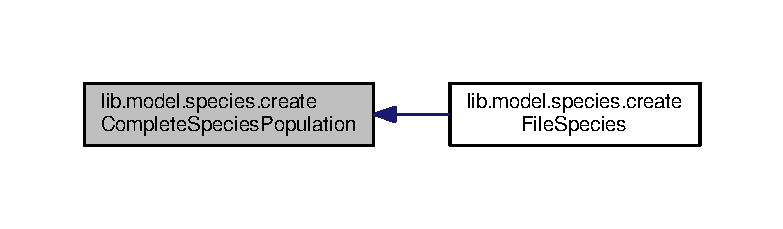
\includegraphics[width=350pt]{a00119_aaa0ed83b7623b65c77b0d583590219ec_icgraph}
\end{center}
\end{figure}


\hypertarget{a00119_a0aab4ec6c7d010b885204f0420072f29}{\index{lib\-::model\-::species@{lib\-::model\-::species}!create\-File\-Species@{create\-File\-Species}}
\index{create\-File\-Species@{create\-File\-Species}!lib::model::species@{lib\-::model\-::species}}
\subsubsection[{create\-File\-Species}]{\setlength{\rightskip}{0pt plus 5cm}def lib.\-model.\-species.\-create\-File\-Species (
\begin{DoxyParamCaption}
\item[{}]{tmp\-Folder, }
\item[{}]{args, }
\item[{}]{pars, }
\item[{}]{tmp\-Scale = {\ttfamily 1}, }
\item[{}]{specieslist = {\ttfamily None}, }
\item[{}]{tmp\-Cat\-In\-R\-A\-F = {\ttfamily None}, }
\item[{}]{tmp\-Raf\-Cat\-Contribute2\-C = {\ttfamily 1}}
\end{DoxyParamCaption}
)}}\label{a00119_a0aab4ec6c7d010b885204f0420072f29}


Definition at line 22 of file species.\-py.



Here is the call graph for this function\-:\nopagebreak
\begin{figure}[H]
\begin{center}
\leavevmode
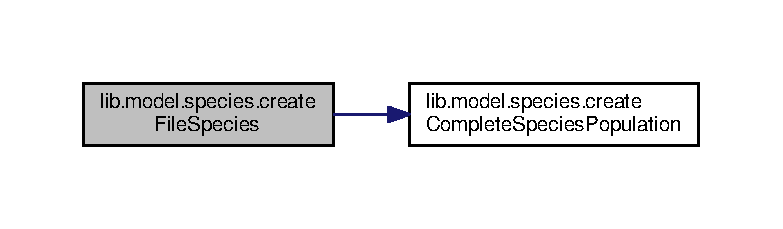
\includegraphics[width=350pt]{a00119_a0aab4ec6c7d010b885204f0420072f29_cgraph}
\end{center}
\end{figure}


\hypertarget{a00119_a1c482d162198854303fbcd154fb1ccbf}{\index{lib\-::model\-::species@{lib\-::model\-::species}!get\-Tot\-Number\-Of\-Species\-From\-Complete\-Pop@{get\-Tot\-Number\-Of\-Species\-From\-Complete\-Pop}}
\index{get\-Tot\-Number\-Of\-Species\-From\-Complete\-Pop@{get\-Tot\-Number\-Of\-Species\-From\-Complete\-Pop}!lib::model::species@{lib\-::model\-::species}}
\subsubsection[{get\-Tot\-Number\-Of\-Species\-From\-Complete\-Pop}]{\setlength{\rightskip}{0pt plus 5cm}def lib.\-model.\-species.\-get\-Tot\-Number\-Of\-Species\-From\-Complete\-Pop (
\begin{DoxyParamCaption}
\item[{}]{M}
\end{DoxyParamCaption}
)}}\label{a00119_a1c482d162198854303fbcd154fb1ccbf}


Definition at line 18 of file species.\-py.

\hypertarget{a00119_a13eb7af04a51ec15dd79ef70fadc93f4}{\index{lib\-::model\-::species@{lib\-::model\-::species}!weighted\-Choice@{weighted\-Choice}}
\index{weighted\-Choice@{weighted\-Choice}!lib::model::species@{lib\-::model\-::species}}
\subsubsection[{weighted\-Choice}]{\setlength{\rightskip}{0pt plus 5cm}def lib.\-model.\-species.\-weighted\-Choice (
\begin{DoxyParamCaption}
\item[{}]{weights, }
\item[{}]{objects}
\end{DoxyParamCaption}
)}}\label{a00119_a13eb7af04a51ec15dd79ef70fadc93f4}
\begin{DoxyVerb}Return a random item from objects, with the weighting defined by weights 
    (which must sum to 1).\end{DoxyVerb}
 

Definition at line 73 of file species.\-py.



Here is the call graph for this function\-:\nopagebreak
\begin{figure}[H]
\begin{center}
\leavevmode
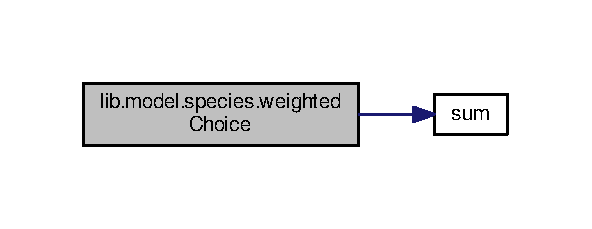
\includegraphics[width=284pt]{a00119_a13eb7af04a51ec15dd79ef70fadc93f4_cgraph}
\end{center}
\end{figure}




\subsection{Variable Documentation}
\hypertarget{a00119_a4a6d118da79b62429ea35b64ef429b11}{\index{lib\-::model\-::species@{lib\-::model\-::species}!\-\_\-\-A\-V\-O\-G\-A\-D\-R\-O\-\_\-@{\-\_\-\-A\-V\-O\-G\-A\-D\-R\-O\-\_\-}}
\index{\-\_\-\-A\-V\-O\-G\-A\-D\-R\-O\-\_\-@{\-\_\-\-A\-V\-O\-G\-A\-D\-R\-O\-\_\-}!lib::model::species@{lib\-::model\-::species}}
\subsubsection[{\-\_\-\-A\-V\-O\-G\-A\-D\-R\-O\-\_\-}]{\setlength{\rightskip}{0pt plus 5cm}float lib.\-model.\-species.\-\_\-\-A\-V\-O\-G\-A\-D\-R\-O\-\_\- = 6.\-022141e23}}\label{a00119_a4a6d118da79b62429ea35b64ef429b11}


Definition at line 10 of file species.\-py.

\hypertarget{a00119_a29a5337ee23b2b7c99866ce2eb49380d}{\index{lib\-::model\-::species@{lib\-::model\-::species}!\-\_\-\-R\-E\-D\-U\-C\-E\-D\-C\-O\-N\-C\-E\-N\-T\-R\-A\-T\-I\-O\-N\-\_\-@{\-\_\-\-R\-E\-D\-U\-C\-E\-D\-C\-O\-N\-C\-E\-N\-T\-R\-A\-T\-I\-O\-N\-\_\-}}
\index{\-\_\-\-R\-E\-D\-U\-C\-E\-D\-C\-O\-N\-C\-E\-N\-T\-R\-A\-T\-I\-O\-N\-\_\-@{\-\_\-\-R\-E\-D\-U\-C\-E\-D\-C\-O\-N\-C\-E\-N\-T\-R\-A\-T\-I\-O\-N\-\_\-}!lib::model::species@{lib\-::model\-::species}}
\subsubsection[{\-\_\-\-R\-E\-D\-U\-C\-E\-D\-C\-O\-N\-C\-E\-N\-T\-R\-A\-T\-I\-O\-N\-\_\-}]{\setlength{\rightskip}{0pt plus 5cm}float lib.\-model.\-species.\-\_\-\-R\-E\-D\-U\-C\-E\-D\-C\-O\-N\-C\-E\-N\-T\-R\-A\-T\-I\-O\-N\-\_\- = 10.\-0}}\label{a00119_a29a5337ee23b2b7c99866ce2eb49380d}


Definition at line 11 of file species.\-py.


\hypertarget{a00121}{\section{reset\-For\-New\-Simulations Namespace Reference}
\label{a00121}\index{reset\-For\-New\-Simulations@{reset\-For\-New\-Simulations}}
}
\subsection*{Functions}
\begin{DoxyCompactItemize}
\item 
def \hyperlink{a00121_aba1c55fe18d1a0b31b346994a7a96628}{zero\-Before\-Str\-Num}
\end{DoxyCompactItemize}
\subsection*{Variables}
\begin{DoxyCompactItemize}
\item 
int \hyperlink{a00121_a60b4005683b2bced2f3e0b22a66abd47}{folders\-S\-I\-M\-S} = 10
\item 
int \hyperlink{a00121_a3869e711bac998c005313abd611c6158}{folders\-R\-E\-P} = 10
\item 
tuple \hyperlink{a00121_a067f416fc59f243e38a0b8a40627979b}{zeros\-S\-I\-M\-S} = \hyperlink{a00121_aba1c55fe18d1a0b31b346994a7a96628}{zero\-Before\-Str\-Num}(\hyperlink{a00071_ad3efca1ea6e3333daf30719ee0501862}{i},\hyperlink{a00121_a60b4005683b2bced2f3e0b22a66abd47}{folders\-S\-I\-M\-S})
\item 
tuple \hyperlink{a00121_a9f88ef39633f68b28f6b0e96d5ebb34c}{zeros\-R\-E\-P\-S} = \hyperlink{a00121_aba1c55fe18d1a0b31b346994a7a96628}{zero\-Before\-Str\-Num}(\hyperlink{a00068_ac86694252f8dfdb19aaeadc4b7c342c6}{j},\hyperlink{a00121_a3869e711bac998c005313abd611c6158}{folders\-R\-E\-P})
\item 
string \hyperlink{a00121_af9fbda1c8e6d13404f0224a5b3ef16fe}{folder\-Name} = \char`\"{}s\-\_\-inv\-\_\-1e-\/2\-\_\-\char`\"{}
\item 
string \hyperlink{a00121_adfad2b3e8459d644a442c254865c564b}{folder\-New} = \char`\"{}s\-\_\-inv\-\_\-1e-\/1\-\_\-\char`\"{}
\item 
tuple \hyperlink{a00121_addd72b08bf24570a2a851808a0b21949}{resdir} = os.\-path.\-join(os.\-curdir, \char`\"{}res\char`\"{})
\item 
tuple \hyperlink{a00121_ad71f20889e7a6394d3c15e5e9381394d}{crt\-Sim\-Folder} = os.\-path.\-join(Str\-To,\hyperlink{a00121_af9fbda1c8e6d13404f0224a5b3ef16fe}{folder\-Name})
\item 
tuple \hyperlink{a00121_a0fd24d58ef8ebf1029176f620ce7fe65}{file\-Dest} = os.\-path.\-join(Str\-To,\hyperlink{a00121_adfad2b3e8459d644a442c254865c564b}{folder\-New},\char`\"{}\-\_\-acsinflux.\-csv\char`\"{})
\item 
tuple \hyperlink{a00121_a876ddf603699b40992ad784167b1121e}{species\-Files} = sorted(glob.\-glob(\char`\"{}species\-\_\-1\-\_\-$\ast$\char`\"{}))
\item 
tuple \hyperlink{a00121_a7a0ded4bf7d86d876a380d82be3c66bd}{mod} = open(\char`\"{}\-\_\-acsspecies.\-csv\char`\"{})
\item 
int \hyperlink{a00121_a9defa7f80f548a96cc89f83a6140727d}{id} = 0
\item 
tuple \hyperlink{a00121_a8479d45d2399e5ddd429e2dc4961204a}{linesplitted} = \hyperlink{a00076_a4d1aa74fac80ae0275c056575fdb6626}{line.\-split}(\char`\"{}\textbackslash{}t\char`\"{})
\item 
tuple \hyperlink{a00121_a3caa9a656a250a12f7112582bde03381}{file} = open(\char`\"{}\-\_\-acsspecies.\-csv\char`\"{}, \char`\"{}w\char`\"{})
\end{DoxyCompactItemize}


\subsection{Function Documentation}
\hypertarget{a00121_aba1c55fe18d1a0b31b346994a7a96628}{\index{reset\-For\-New\-Simulations@{reset\-For\-New\-Simulations}!zero\-Before\-Str\-Num@{zero\-Before\-Str\-Num}}
\index{zero\-Before\-Str\-Num@{zero\-Before\-Str\-Num}!resetForNewSimulations@{reset\-For\-New\-Simulations}}
\subsubsection[{zero\-Before\-Str\-Num}]{\setlength{\rightskip}{0pt plus 5cm}def reset\-For\-New\-Simulations.\-zero\-Before\-Str\-Num (
\begin{DoxyParamCaption}
\item[{}]{tmpl, }
\item[{}]{tmp\-L}
\end{DoxyParamCaption}
)}}\label{a00121_aba1c55fe18d1a0b31b346994a7a96628}


Definition at line 5 of file reset\-For\-New\-Simulations.\-py.



\subsection{Variable Documentation}
\hypertarget{a00121_ad71f20889e7a6394d3c15e5e9381394d}{\index{reset\-For\-New\-Simulations@{reset\-For\-New\-Simulations}!crt\-Sim\-Folder@{crt\-Sim\-Folder}}
\index{crt\-Sim\-Folder@{crt\-Sim\-Folder}!resetForNewSimulations@{reset\-For\-New\-Simulations}}
\subsubsection[{crt\-Sim\-Folder}]{\setlength{\rightskip}{0pt plus 5cm}tuple reset\-For\-New\-Simulations.\-crt\-Sim\-Folder = os.\-path.\-join(Str\-To,{\bf folder\-Name})}}\label{a00121_ad71f20889e7a6394d3c15e5e9381394d}


Definition at line 51 of file reset\-For\-New\-Simulations.\-py.

\hypertarget{a00121_a3caa9a656a250a12f7112582bde03381}{\index{reset\-For\-New\-Simulations@{reset\-For\-New\-Simulations}!file@{file}}
\index{file@{file}!resetForNewSimulations@{reset\-For\-New\-Simulations}}
\subsubsection[{file}]{\setlength{\rightskip}{0pt plus 5cm}tuple reset\-For\-New\-Simulations.\-file = open(\char`\"{}\-\_\-acsspecies.\-csv\char`\"{}, \char`\"{}w\char`\"{})}}\label{a00121_a3caa9a656a250a12f7112582bde03381}


Definition at line 99 of file reset\-For\-New\-Simulations.\-py.

\hypertarget{a00121_a0fd24d58ef8ebf1029176f620ce7fe65}{\index{reset\-For\-New\-Simulations@{reset\-For\-New\-Simulations}!file\-Dest@{file\-Dest}}
\index{file\-Dest@{file\-Dest}!resetForNewSimulations@{reset\-For\-New\-Simulations}}
\subsubsection[{file\-Dest}]{\setlength{\rightskip}{0pt plus 5cm}tuple reset\-For\-New\-Simulations.\-file\-Dest = os.\-path.\-join(Str\-To,{\bf folder\-New},\char`\"{}\-\_\-acsinflux.\-csv\char`\"{})}}\label{a00121_a0fd24d58ef8ebf1029176f620ce7fe65}


Definition at line 57 of file reset\-For\-New\-Simulations.\-py.

\hypertarget{a00121_af9fbda1c8e6d13404f0224a5b3ef16fe}{\index{reset\-For\-New\-Simulations@{reset\-For\-New\-Simulations}!folder\-Name@{folder\-Name}}
\index{folder\-Name@{folder\-Name}!resetForNewSimulations@{reset\-For\-New\-Simulations}}
\subsubsection[{folder\-Name}]{\setlength{\rightskip}{0pt plus 5cm}string reset\-For\-New\-Simulations.\-folder\-Name = \char`\"{}s\-\_\-inv\-\_\-1e-\/2\-\_\-\char`\"{}}}\label{a00121_af9fbda1c8e6d13404f0224a5b3ef16fe}


Definition at line 31 of file reset\-For\-New\-Simulations.\-py.

\hypertarget{a00121_adfad2b3e8459d644a442c254865c564b}{\index{reset\-For\-New\-Simulations@{reset\-For\-New\-Simulations}!folder\-New@{folder\-New}}
\index{folder\-New@{folder\-New}!resetForNewSimulations@{reset\-For\-New\-Simulations}}
\subsubsection[{folder\-New}]{\setlength{\rightskip}{0pt plus 5cm}string reset\-For\-New\-Simulations.\-folder\-New = \char`\"{}s\-\_\-inv\-\_\-1e-\/1\-\_\-\char`\"{}}}\label{a00121_adfad2b3e8459d644a442c254865c564b}


Definition at line 32 of file reset\-For\-New\-Simulations.\-py.

\hypertarget{a00121_a3869e711bac998c005313abd611c6158}{\index{reset\-For\-New\-Simulations@{reset\-For\-New\-Simulations}!folders\-R\-E\-P@{folders\-R\-E\-P}}
\index{folders\-R\-E\-P@{folders\-R\-E\-P}!resetForNewSimulations@{reset\-For\-New\-Simulations}}
\subsubsection[{folders\-R\-E\-P}]{\setlength{\rightskip}{0pt plus 5cm}int reset\-For\-New\-Simulations.\-folders\-R\-E\-P = 10}}\label{a00121_a3869e711bac998c005313abd611c6158}


Definition at line 22 of file reset\-For\-New\-Simulations.\-py.

\hypertarget{a00121_a60b4005683b2bced2f3e0b22a66abd47}{\index{reset\-For\-New\-Simulations@{reset\-For\-New\-Simulations}!folders\-S\-I\-M\-S@{folders\-S\-I\-M\-S}}
\index{folders\-S\-I\-M\-S@{folders\-S\-I\-M\-S}!resetForNewSimulations@{reset\-For\-New\-Simulations}}
\subsubsection[{folders\-S\-I\-M\-S}]{\setlength{\rightskip}{0pt plus 5cm}int reset\-For\-New\-Simulations.\-folders\-S\-I\-M\-S = 10}}\label{a00121_a60b4005683b2bced2f3e0b22a66abd47}


Definition at line 21 of file reset\-For\-New\-Simulations.\-py.

\hypertarget{a00121_a9defa7f80f548a96cc89f83a6140727d}{\index{reset\-For\-New\-Simulations@{reset\-For\-New\-Simulations}!id@{id}}
\index{id@{id}!resetForNewSimulations@{reset\-For\-New\-Simulations}}
\subsubsection[{id}]{\setlength{\rightskip}{0pt plus 5cm}int reset\-For\-New\-Simulations.\-id = 0}}\label{a00121_a9defa7f80f548a96cc89f83a6140727d}


Definition at line 83 of file reset\-For\-New\-Simulations.\-py.

\hypertarget{a00121_a8479d45d2399e5ddd429e2dc4961204a}{\index{reset\-For\-New\-Simulations@{reset\-For\-New\-Simulations}!linesplitted@{linesplitted}}
\index{linesplitted@{linesplitted}!resetForNewSimulations@{reset\-For\-New\-Simulations}}
\subsubsection[{linesplitted}]{\setlength{\rightskip}{0pt plus 5cm}tuple reset\-For\-New\-Simulations.\-linesplitted = {\bf line.\-split}(\char`\"{}\textbackslash{}t\char`\"{})}}\label{a00121_a8479d45d2399e5ddd429e2dc4961204a}


Definition at line 85 of file reset\-For\-New\-Simulations.\-py.

\hypertarget{a00121_a7a0ded4bf7d86d876a380d82be3c66bd}{\index{reset\-For\-New\-Simulations@{reset\-For\-New\-Simulations}!mod@{mod}}
\index{mod@{mod}!resetForNewSimulations@{reset\-For\-New\-Simulations}}
\subsubsection[{mod}]{\setlength{\rightskip}{0pt plus 5cm}tuple reset\-For\-New\-Simulations.\-mod = open(\char`\"{}\-\_\-acsspecies.\-csv\char`\"{})}}\label{a00121_a7a0ded4bf7d86d876a380d82be3c66bd}


Definition at line 82 of file reset\-For\-New\-Simulations.\-py.

\hypertarget{a00121_addd72b08bf24570a2a851808a0b21949}{\index{reset\-For\-New\-Simulations@{reset\-For\-New\-Simulations}!resdir@{resdir}}
\index{resdir@{resdir}!resetForNewSimulations@{reset\-For\-New\-Simulations}}
\subsubsection[{resdir}]{\setlength{\rightskip}{0pt plus 5cm}tuple reset\-For\-New\-Simulations.\-resdir = os.\-path.\-join(os.\-curdir, \char`\"{}res\char`\"{})}}\label{a00121_addd72b08bf24570a2a851808a0b21949}


Definition at line 42 of file reset\-For\-New\-Simulations.\-py.

\hypertarget{a00121_a876ddf603699b40992ad784167b1121e}{\index{reset\-For\-New\-Simulations@{reset\-For\-New\-Simulations}!species\-Files@{species\-Files}}
\index{species\-Files@{species\-Files}!resetForNewSimulations@{reset\-For\-New\-Simulations}}
\subsubsection[{species\-Files}]{\setlength{\rightskip}{0pt plus 5cm}tuple reset\-For\-New\-Simulations.\-species\-Files = sorted(glob.\-glob(\char`\"{}species\-\_\-1\-\_\-$\ast$\char`\"{}))}}\label{a00121_a876ddf603699b40992ad784167b1121e}


Definition at line 66 of file reset\-For\-New\-Simulations.\-py.

\hypertarget{a00121_a9f88ef39633f68b28f6b0e96d5ebb34c}{\index{reset\-For\-New\-Simulations@{reset\-For\-New\-Simulations}!zeros\-R\-E\-P\-S@{zeros\-R\-E\-P\-S}}
\index{zeros\-R\-E\-P\-S@{zeros\-R\-E\-P\-S}!resetForNewSimulations@{reset\-For\-New\-Simulations}}
\subsubsection[{zeros\-R\-E\-P\-S}]{\setlength{\rightskip}{0pt plus 5cm}tuple reset\-For\-New\-Simulations.\-zeros\-R\-E\-P\-S = {\bf zero\-Before\-Str\-Num}({\bf j},{\bf folders\-R\-E\-P})}}\label{a00121_a9f88ef39633f68b28f6b0e96d5ebb34c}


Definition at line 29 of file reset\-For\-New\-Simulations.\-py.

\hypertarget{a00121_a067f416fc59f243e38a0b8a40627979b}{\index{reset\-For\-New\-Simulations@{reset\-For\-New\-Simulations}!zeros\-S\-I\-M\-S@{zeros\-S\-I\-M\-S}}
\index{zeros\-S\-I\-M\-S@{zeros\-S\-I\-M\-S}!resetForNewSimulations@{reset\-For\-New\-Simulations}}
\subsubsection[{zeros\-S\-I\-M\-S}]{\setlength{\rightskip}{0pt plus 5cm}tuple reset\-For\-New\-Simulations.\-zeros\-S\-I\-M\-S = {\bf zero\-Before\-Str\-Num}({\bf i},{\bf folders\-S\-I\-M\-S})}}\label{a00121_a067f416fc59f243e38a0b8a40627979b}


Definition at line 28 of file reset\-For\-New\-Simulations.\-py.


\chapter{Class Documentation}
\hypertarget{a00012}{\section{common\+Functions Class Reference}
\label{a00012}\index{common\+Functions@{common\+Functions}}
}


This class contains all the common function of the system.  




{\ttfamily \#include $<$common\+Functions.\+h$>$}



\subsection{Detailed Description}
This class contains all the common function of the system. 

This class contains all the functions useful in general \begin{DoxyAuthor}{Authors}
alessandro filisetti 
\end{DoxyAuthor}
\begin{DoxyDate}{Date}
2011/12/10 
\end{DoxyDate}
\begin{DoxyVersion}{Version}
1.\+0 
\end{DoxyVersion}


The documentation for this class was generated from the following file\+:\begin{DoxyCompactItemize}
\item 
/\+Users/alessandrofilisetti/\+Documents/\+G\+I\+T/carness/\+\_\+analysis/python\+Tools/init/exps/source\+Code/\hyperlink{a00058}{common\+Functions.\+h}\end{DoxyCompactItemize}

\hypertarget{a00013}{\section{environment Class Reference}
\label{a00013}\index{environment@{environment}}
}


environment class  




{\ttfamily \#include $<$environment.\+h$>$}

\subsection*{Public Member Functions}
\begin{DoxyCompactItemize}
\item 
\hyperlink{a00013_aa44bbabec52bf2d61a19685a30e68de1}{environment} (string tmp\+Initial\+Path)
\item 
\hyperlink{a00013_ae323954bd5b674bf34d954c3f7b67629}{$\sim$environment} ()
\item 
\hyperlink{a00050_a8d277355641a098190360234e2ebde35}{acs\+\_\+int} \hyperlink{a00013_afad68362d5f4ec0689941e3c1b92c2e8}{get\+Ngen} () const 
\item 
\hyperlink{a00050_a8d277355641a098190360234e2ebde35}{acs\+\_\+int} \hyperlink{a00013_a5a8522899b3e84b9c394d5d83d1e5c63}{get\+Nsim} () const 
\item 
\hyperlink{a00050_ab776853a005fcbf56af0424a2a4dd607}{acs\+\_\+double} \hyperlink{a00013_a14bad649a73246617361f0e1765f49f8}{get\+Actual\+Time} () const 
\item 
\hyperlink{a00050_ab776853a005fcbf56af0424a2a4dd607}{acs\+\_\+double} \hyperlink{a00013_aa850c2805e508b2aac4fbd5d5f9de77b}{get\+Nseconds} () const 
\item 
\hyperlink{a00050_a8d277355641a098190360234e2ebde35}{acs\+\_\+int} \hyperlink{a00013_a5cb9cf3968f19e23f6c54f4c915cf878}{get\+Nreactions} () const 
\item 
\hyperlink{a00050_ab776853a005fcbf56af0424a2a4dd607}{acs\+\_\+double} \hyperlink{a00013_af2b482132fc3ab299118f7a894bd53a2}{get\+M\+A\+Xhours} () const 
\item 
\hyperlink{a00050_a8d277355641a098190360234e2ebde35}{acs\+\_\+int} \hyperlink{a00013_ae626b961a53eeb5e08b4190da235e8dd}{get\+M\+A\+Xattempts} () const 
\item 
\hyperlink{a00050_a8d277355641a098190360234e2ebde35}{acs\+\_\+int} \hyperlink{a00013_a0851e3481e6fec7f4feef126d5a6704c}{get\+Current\+Attempts} () const 
\item 
\hyperlink{a00050_ab776853a005fcbf56af0424a2a4dd607}{acs\+\_\+double} \hyperlink{a00013_a892dd7bd29342c4206c39556d91a83da}{get\+Time\+Structures\+Saving\+Interval} () const 
\item 
\hyperlink{a00050_ab776853a005fcbf56af0424a2a4dd607}{acs\+\_\+double} \hyperlink{a00013_a77e995bee54ab4e09f165a857a7b0272}{get\+File\+Times\+Saving\+Interval} () const 
\item 
\hyperlink{a00050_a8d277355641a098190360234e2ebde35}{acs\+\_\+int} \hyperlink{a00013_a984f79e5f89b774b65db901899687ac0}{get\+Last\+Firing\+Disk\+Species\+I\+D} () const 
\item 
\hyperlink{a00050_ab776853a005fcbf56af0424a2a4dd607}{acs\+\_\+double} \hyperlink{a00013_a8bea373c48982a78ee46c5c5fafcb81c}{get\+Overall\+Concentration} () const 
\item 
\hyperlink{a00050_a8d277355641a098190360234e2ebde35}{acs\+\_\+int} \hyperlink{a00013_aca760caf9354f541020c1db58490b18f}{get\+Max\+Non\+Catalytic\+Length} () const 
\item 
\hyperlink{a00050_ab776853a005fcbf56af0424a2a4dd607}{acs\+\_\+double} \hyperlink{a00013_ae244aa972cf10c103b8b20d95703831f}{get\+Rct\+Prob} () const 
\item 
\hyperlink{a00050_ab776853a005fcbf56af0424a2a4dd607}{acs\+\_\+double} \hyperlink{a00013_ac728f6ab012c42fa85a2e2f70df7dc58}{get\+Cleav\+Prob} () const 
\item 
bool \hyperlink{a00013_a2a2ac2a8140df67688a71d3349adf04a}{get\+Reverse\+Reactions} () const 
\item 
\hyperlink{a00050_a8d277355641a098190360234e2ebde35}{acs\+\_\+int} \hyperlink{a00013_ab463a460de102c79c1044ab8a2c176ae}{get\+Energy} () const 
\item 
\hyperlink{a00050_ab776853a005fcbf56af0424a2a4dd607}{acs\+\_\+double} \hyperlink{a00013_a4fcc6030b68a37bedff870b9c48c188d}{get\+Ratio\+Species\+Energizable} () const 
\item 
\hyperlink{a00050_a8d277355641a098190360234e2ebde35}{acs\+\_\+int} \hyperlink{a00013_a69d18914fe7c8e96b10992668960b83b}{get\+A\+D\+P} () const 
\item 
\hyperlink{a00050_a8d277355641a098190360234e2ebde35}{acs\+\_\+int} \hyperlink{a00013_a02346c5d824e83e0a76dd01f4672ad8b}{get\+A\+T\+P} () const 
\item 
\hyperlink{a00050_a19319d75f02db4308bc5c0026d98cd85}{acs\+\_\+long\+Int} \hyperlink{a00013_a5a2ee72147144e7a04f4b363f1cc0914}{get\+Mols} () const 
\item 
\hyperlink{a00050_a19319d75f02db4308bc5c0026d98cd85}{acs\+\_\+long\+Int} \hyperlink{a00013_a57e1eb6043a54fbebd2ac01ebdac9fa1}{get\+New\+Mols} () const 
\item 
\hyperlink{a00050_a19319d75f02db4308bc5c0026d98cd85}{acs\+\_\+long\+Int} \hyperlink{a00013_aebc2bf6d400686a73dae1f6162cfeadc}{get\+Nspecies} () const 
\item 
\hyperlink{a00050_a19319d75f02db4308bc5c0026d98cd85}{acs\+\_\+long\+Int} \hyperlink{a00013_a4a2b21d139acc93ae0fdf29c8b025cce}{get\+Nnew\+Species} () const 
\item 
\hyperlink{a00050_a19319d75f02db4308bc5c0026d98cd85}{acs\+\_\+long\+Int} \hyperlink{a00013_a5f6c40cbf788d58db588dc6280f0174f}{get\+Ncpx} () const 
\item 
\hyperlink{a00050_a19319d75f02db4308bc5c0026d98cd85}{acs\+\_\+long\+Int} \hyperlink{a00013_a39bb98a336b69f25479b8f82b9928bd3}{get\+Ncpx\+Mols} () const 
\item 
\hyperlink{a00050_ab776853a005fcbf56af0424a2a4dd607}{acs\+\_\+double} \hyperlink{a00013_a389a70abe42c7652c9511b7ed3b974c0}{get\+Gillespie\+Mean} () const 
\item 
\hyperlink{a00050_ab776853a005fcbf56af0424a2a4dd607}{acs\+\_\+double} \hyperlink{a00013_a41d9f79794b74845f2d00b4c0affea02}{getgillespie\+S\+D} () const 
\item 
\hyperlink{a00050_ab776853a005fcbf56af0424a2a4dd607}{acs\+\_\+double} \hyperlink{a00013_af4cba1a1f9c1c0106241ca5338b7906d}{getgillespie\+Entropy} () const 
\item 
\hyperlink{a00050_ab776853a005fcbf56af0424a2a4dd607}{acs\+\_\+double} \hyperlink{a00013_a98a4989029d77e99cf2ca9fb0eb1c2ab}{get\+Ratio\+Between\+New\+Gill\+Tot\+Gill} () const 
\item 
\hyperlink{a00050_ab776853a005fcbf56af0424a2a4dd607}{acs\+\_\+double} \hyperlink{a00013_aa0e7940868932ac4b26fd61943952528}{get\+Ratio\+Between\+Backand\+Forw} () const 
\item 
bool \hyperlink{a00013_a883327bbb969164eb8b3c2d1c941ca03}{get\+System\+Exp\+Flag} () const 
\item 
\hyperlink{a00050_ab776853a005fcbf56af0424a2a4dd607}{acs\+\_\+double} \hyperlink{a00013_ab429d2057ee1092bf210c29e70153f75}{get\+Kdiss} () const 
\item 
\hyperlink{a00050_ab776853a005fcbf56af0424a2a4dd607}{acs\+\_\+double} \hyperlink{a00013_aa862f1f98c6060747d6f1f30377671ff}{get\+Kass} () const 
\item 
\hyperlink{a00050_ab776853a005fcbf56af0424a2a4dd607}{acs\+\_\+double} \hyperlink{a00013_ac62c6b719db59d5829e3cc451b237f44}{get\+Kcpx} () const 
\item 
\hyperlink{a00050_ab776853a005fcbf56af0424a2a4dd607}{acs\+\_\+double} \hyperlink{a00013_a9091c4a0fe31f6d5f5330e7ebff297a3}{get\+Kcpx\+Diss} () const 
\item 
\hyperlink{a00050_ab776853a005fcbf56af0424a2a4dd607}{acs\+\_\+double} \hyperlink{a00013_a7615c746521a592ff1ab2d0793b14d89}{get\+Knrg} () const 
\item 
\hyperlink{a00050_ab776853a005fcbf56af0424a2a4dd607}{acs\+\_\+double} \hyperlink{a00013_a4c163b36e84cd8406aff4ab5d220a251}{get\+Kirrad} () const 
\item 
\hyperlink{a00050_ab776853a005fcbf56af0424a2a4dd607}{acs\+\_\+double} \hyperlink{a00013_a2c6ca24592b5feab891e43233c581711}{get\+K\+\_\+spont\+\_\+diss} () const 
\item 
\hyperlink{a00050_ab776853a005fcbf56af0424a2a4dd607}{acs\+\_\+double} \hyperlink{a00013_a6557765370b636bc7d4e02288b444c0e}{get\+K\+\_\+spont\+\_\+ass} () const 
\item 
\hyperlink{a00050_ab776853a005fcbf56af0424a2a4dd607}{acs\+\_\+double} \hyperlink{a00013_a771963196a27d3532cd7af4b98a5a9c5}{get\+Cleavage\+K\+C} () const 
\item 
\hyperlink{a00050_ab776853a005fcbf56af0424a2a4dd607}{acs\+\_\+double} \hyperlink{a00013_abf3168adf05ff9fa6bab4e34b387f0a6}{get\+Complex\+K\+C} () const 
\item 
\hyperlink{a00050_ab776853a005fcbf56af0424a2a4dd607}{acs\+\_\+double} \hyperlink{a00013_a7ac1b69dd38107d5c40339563969d09f}{get\+Condensation\+K\+C} () const 
\item 
\hyperlink{a00050_ab776853a005fcbf56af0424a2a4dd607}{acs\+\_\+double} \hyperlink{a00013_ae58bcd60ae01a8ba12f83c1328121c35}{get\+Complex\+Deg\+K\+C} () const 
\item 
\hyperlink{a00050_ab776853a005fcbf56af0424a2a4dd607}{acs\+\_\+double} \hyperlink{a00013_a4ed6ad35297e718398fb42a2b9dbe4ae}{get\+Molecule\+Decay\+K\+C} () const 
\item 
\hyperlink{a00050_a8d277355641a098190360234e2ebde35}{acs\+\_\+int} \hyperlink{a00013_a4c58b3ce555f04f009bcfb7bbc2b0000}{get\+Max\+L\+Out} () const 
\item 
\hyperlink{a00050_a8d277355641a098190360234e2ebde35}{acs\+\_\+int} \hyperlink{a00013_a6df38337d38f2f714be7058a2a31202c}{get\+Solubility\+Threshold} () const 
\item 
\hyperlink{a00050_ab776853a005fcbf56af0424a2a4dd607}{acs\+\_\+double} \hyperlink{a00013_a46193e153bd5dcc37fb35346cb7fd971}{get\+Diffusion\+Contribute} () const 
\item 
\hyperlink{a00050_ab776853a005fcbf56af0424a2a4dd607}{acs\+\_\+double} \hyperlink{a00013_a6f0b4481779cd12dbcd8155916c7d703}{get\+Influx} () const 
\item 
\hyperlink{a00050_ab776853a005fcbf56af0424a2a4dd607}{acs\+\_\+double} \hyperlink{a00013_a469a7ce80a1e9e5fae77b46b66dfee18}{get\+Refill\+Interval} () const 
\item 
string \hyperlink{a00013_add8478cfc878c3aa5a57b2a71357a088}{get\+Alphabet} () const 
\item 
\hyperlink{a00050_ab776853a005fcbf56af0424a2a4dd607}{acs\+\_\+double} \hyperlink{a00013_a355b53cbc86aaab2a6d114980162ac0e}{get\+Volume} () const 
\item 
\hyperlink{a00050_ab776853a005fcbf56af0424a2a4dd607}{acs\+\_\+double} \hyperlink{a00013_ab6952f7f6fd971ece0a8661733cfc2b3}{get\+Random\+Seed} () const 
\item 
vector$<$ \hyperlink{a00021}{species} $>$ \hyperlink{a00013_adb12eb52af74ea1fdfe0cd195109fe83}{get\+Molecules\+Population} () const 
\item 
\hyperlink{a00050_a19319d75f02db4308bc5c0026d98cd85}{acs\+\_\+long\+Int} \hyperlink{a00013_a7a321296874fa1320da225cdbbf56a64}{get\+Total\+Number\+Of\+Species} ()
\item 
\hyperlink{a00050_a19319d75f02db4308bc5c0026d98cd85}{acs\+\_\+long\+Int} \hyperlink{a00013_a8796aead7bcc4a3f91eec7bc908dfa5b}{get\+Total\+Number\+Of\+Possible\+Catalysts} ()
\item 
\hyperlink{a00050_a19319d75f02db4308bc5c0026d98cd85}{acs\+\_\+long\+Int} \hyperlink{a00013_a57e7ac49955f4717096cb6696ee03a61}{get\+Total\+Number\+Of\+Molecules} ()
\item 
\hyperlink{a00050_a19319d75f02db4308bc5c0026d98cd85}{acs\+\_\+long\+Int} \hyperlink{a00013_a453d88017912e8b5973310ea2b044266}{get\+Total\+Number\+Of\+Complex\+Species} ()
\item 
\hyperlink{a00050_a19319d75f02db4308bc5c0026d98cd85}{acs\+\_\+long\+Int} \hyperlink{a00013_ab564c7ddffd3dba896d5b049e1257793}{get\+Total\+Number\+Of\+Complexes} ()
\item 
\hyperlink{a00050_a19319d75f02db4308bc5c0026d98cd85}{acs\+\_\+long\+Int} \hyperlink{a00013_aa8c94019533639038f99587fc2b029dc}{get\+Total\+Number\+Of\+Monomers} ()
\item 
vector$<$ \hyperlink{a00020}{reactions} $>$ \hyperlink{a00013_a3d44f3f4a8f9010fa99c49f5cc961416}{get\+Reactions\+Layer} () const 
\item 
int \hyperlink{a00013_a2de42381b0b9cba889bbb95c1456cfe5}{get\+Debug\+Level} () const 
\item 
\hyperlink{a00050_a19319d75f02db4308bc5c0026d98cd85}{acs\+\_\+long\+Int} \hyperlink{a00013_ab98d4ad28b101f08279aa3458d5dfda3}{get\+Number\+Of\+Theoretical\+Species} () const 
\item 
\hyperlink{a00050_a19319d75f02db4308bc5c0026d98cd85}{acs\+\_\+long\+Int} \hyperlink{a00013_abf45b6406f8c0e95c4c5edf6b374e112}{get\+Number\+Of\+Reactions} () const 
\item 
\hyperlink{a00050_a19319d75f02db4308bc5c0026d98cd85}{acs\+\_\+long\+Int} \hyperlink{a00013_a21609adb1a83a4cb7eaec78a90acd624}{get\+Number\+Of\+Catalysis} () const 
\item 
\hyperlink{a00050_a19319d75f02db4308bc5c0026d98cd85}{acs\+\_\+long\+Int} \hyperlink{a00013_a79255c58733b08407dc81d89e306d74f}{get\+Number\+Of\+Gillespie\+C\+O\+P\+Ypossible\+Rcts} () const 
\item 
\hyperlink{a00050_a19319d75f02db4308bc5c0026d98cd85}{acs\+\_\+long\+Int} \hyperlink{a00013_a3140242018e8232dfa89a127ac1bb282}{get\+Number\+Of\+Gillespie\+Possible\+Rcts} () const 
\item 
void \hyperlink{a00013_a4fb98d7cad06ef479e2643785231feb9}{set\+Living\+Species\+I\+Ds\+And\+Amounts} ()
\item 
void \hyperlink{a00013_ac5528a39937cdc76f0dd23c27542110c}{set\+Not\+Charged\+And\+Charged\+Species\+I\+Ds\+And\+Amounts} ()
\item 
\hyperlink{a00050_a19319d75f02db4308bc5c0026d98cd85}{acs\+\_\+long\+Int} \hyperlink{a00013_a8b9a3b5c5a2f86206c5fb124352e366e}{get\+Cleavage\+Counter} () const 
\item 
\hyperlink{a00050_a19319d75f02db4308bc5c0026d98cd85}{acs\+\_\+long\+Int} \hyperlink{a00013_aa2ded3c5ba8c4ce41ee86399dc616d4a}{get\+Endo\+Cleavage\+Counter} () const 
\item 
\hyperlink{a00050_a19319d75f02db4308bc5c0026d98cd85}{acs\+\_\+long\+Int} \hyperlink{a00013_a0fc62131bf552c2a995c7ddc461828cd}{get\+Condensation\+Counter} () const 
\item 
\hyperlink{a00050_a19319d75f02db4308bc5c0026d98cd85}{acs\+\_\+long\+Int} \hyperlink{a00013_aaa23d550cfa37344dd3bb4d5767e6ea0}{get\+Endo\+Condensation\+Counter} () const 
\item 
\hyperlink{a00050_a19319d75f02db4308bc5c0026d98cd85}{acs\+\_\+long\+Int} \hyperlink{a00013_a5d72675f37c3936c58d27480613a9ab6}{get\+Cpx\+Form\+Counter} () const 
\item 
\hyperlink{a00050_a19319d75f02db4308bc5c0026d98cd85}{acs\+\_\+long\+Int} \hyperlink{a00013_abf2f63b22c52e17f6089f098651584b8}{get\+Cpx\+Diss\+Counter} () const 
\item 
\hyperlink{a00050_a19319d75f02db4308bc5c0026d98cd85}{acs\+\_\+long\+Int} \hyperlink{a00013_a75329459280bc79537a5c08883449a63}{get\+Overall\+Loaded\+Mols\+Counter} () const 
\item 
\hyperlink{a00050_a19319d75f02db4308bc5c0026d98cd85}{acs\+\_\+long\+Int} \hyperlink{a00013_a914378e80f148a4b24fc8e27ebb02198}{get\+Spont\+Diss\+Counter} () const 
\item 
\hyperlink{a00050_a19319d75f02db4308bc5c0026d98cd85}{acs\+\_\+long\+Int} \hyperlink{a00013_ab3c423ac69aac398c087cde1dcb0dccb}{get\+Spont\+Ass\+Counter} () const 
\item 
\hyperlink{a00050_a8d277355641a098190360234e2ebde35}{acs\+\_\+int} \hyperlink{a00013_aadb5c442d5c9d16a0d6b2e90715dda94}{get\+Tot\+Number\+Of\+Charged\+Mols} ()
\item 
void \hyperlink{a00013_af959a6b6a72cb6226fef7f0e7fab5c0c}{show\+Global\+Parameter} ()
\item 
void \hyperlink{a00013_a429c2529badaeda72e553f500b990e11}{print\+Initial\+Condition} ()
\item 
void \hyperlink{a00013_a48d8fd9d8d5c9c31f0b4af87c8cbd28f}{print\+All\+Species\+Id\+And\+Sequence} ()
\item 
void \hyperlink{a00013_aa3a18c59f6127c642603a98c1b3a2224}{print\+Gillespie\+Structure} ()
\item 
void \hyperlink{a00013_ad8fcefe5325382fb307627c7e8362ba8}{print\+Nutrients\+And\+Probability} ()
\item 
void \hyperlink{a00013_af579052ed051a2e3516218220d238303}{print\+All\+Charge\+Mols} ()
\item 
bool \hyperlink{a00013_aee77384e63261db28ef5677844bdbaf6}{create\+Initial\+Molecules\+Population\+From\+File\+S\+T\+D} (string tmp\+Species\+File\+Path)
\item 
bool \hyperlink{a00013_a2f181e0d3ad1e8062ba0a8c9358ebc58}{create\+Initial\+Reactions\+Layer\+From\+File\+S\+T\+D} (string tmp\+Species\+File\+Path)
\item 
bool \hyperlink{a00013_a29eeb7a1b4689c10fd872e82179b4d84}{create\+Initial\+Catalysis\+Layer\+From\+File\+S\+T\+D} (string tmp\+Catalysis\+File\+Path)
\item 
bool \hyperlink{a00013_a902df40829dad9a885122082ec8fff7a}{create\+Influx\+Layers\+From\+File\+S\+T\+D} (string tmp\+Influx\+File\+Path)
\item 
bool \hyperlink{a00013_abe1a616460ea328067874df715679319}{create\+Nrg\+Boolean\+Functions\+From\+File\+S\+T\+D} (string tmp\+Bool\+Nrg\+File\+Path)
\item 
bool \hyperlink{a00013_aa70e1394bf2240f6e5f14d4cbf369a3b}{create\+Initial\+Molecules\+Population\+From\+Specific\+File\+S\+T\+D} (string tmp\+Species\+File\+Path, \hyperlink{a00050_a8d277355641a098190360234e2ebde35}{acs\+\_\+int} tmp\+Act\+G\+E\+N, \hyperlink{a00050_a8d277355641a098190360234e2ebde35}{acs\+\_\+int} tmp\+Act\+S\+I\+M)
\item 
bool \hyperlink{a00013_a743956229b11d7860dbc89a18f869586}{create\+Initial\+Reactions\+Layer\+From\+Specific\+File\+S\+T\+D} (string tmp\+Reactions\+File\+Path, \hyperlink{a00050_a8d277355641a098190360234e2ebde35}{acs\+\_\+int} tmp\+Act\+G\+E\+N, \hyperlink{a00050_a8d277355641a098190360234e2ebde35}{acs\+\_\+int} tmp\+Act\+S\+I\+M)
\item 
bool \hyperlink{a00013_a6dd31bae82367ebe7d6a6bb062b8cd07}{create\+Initial\+Catalysis\+Layer\+From\+Specific\+File\+S\+T\+D} (string tmp\+Catalysis\+File\+Path, \hyperlink{a00050_a8d277355641a098190360234e2ebde35}{acs\+\_\+int} tmp\+Act\+G\+E\+N, \hyperlink{a00050_a8d277355641a098190360234e2ebde35}{acs\+\_\+int} tmp\+Act\+S\+I\+M)
\item 
void \hyperlink{a00013_a9ceec5e00b0f5a51dd125c583b8ac5ec}{nutrients\+Amounts\+Fixing} ()
\item 
\hyperlink{a00050_a8d277355641a098190360234e2ebde35}{acs\+\_\+int} \hyperlink{a00013_a0fd3cb062d35d2f6dd8961e95dd477b7}{compute\+Sng\+Species\+Rcts\+Number} (\hyperlink{a00050_a19319d75f02db4308bc5c0026d98cd85}{acs\+\_\+long\+Int} tmp\+Total\+Number\+Of\+Reactions, \hyperlink{a00015}{M\+T\+Rand} \&tmp\+Rnd\+Double\+Gen)
\item 
\hyperlink{a00050_a8d277355641a098190360234e2ebde35}{acs\+\_\+int} \hyperlink{a00013_a53282cca8882e86652ab0a22e6966d17}{select\+Whether\+Cleavage\+Or\+Cond} (\hyperlink{a00015}{M\+T\+Rand} \&tmp\+\_\+\+\_\+\+Rnd\+Double\+Gen)
\item 
bool \hyperlink{a00013_a76794f37d6d94b7504c58f0f4a4709ca}{create\+Reactions\+For\+This\+Species} (\hyperlink{a00050_a19319d75f02db4308bc5c0026d98cd85}{acs\+\_\+long\+Int} tmps\+I\+D, \hyperlink{a00050_a8d277355641a098190360234e2ebde35}{acs\+\_\+int} tmp\+Reactions\+For\+This\+Species, \hyperlink{a00015}{M\+T\+Rand} \&tmp\+\_\+\+Rnd\+Double\+Gen, vector$<$ \hyperlink{a00050_a19319d75f02db4308bc5c0026d98cd85}{acs\+\_\+long\+Int} $>$ \&tmp\+I\+D\+Of\+Candidate\+Species, \hyperlink{a00050_a8d277355641a098190360234e2ebde35}{acs\+\_\+int} tmp\+Rct\+Creation\+Type)
\item 
bool \hyperlink{a00013_ace92235425bfbe692e3873ba5bb07639}{update\+Reactions} (\hyperlink{a00050_a19319d75f02db4308bc5c0026d98cd85}{acs\+\_\+long\+Int} tmp\+I\+Dto\+Update, \hyperlink{a00050_a19319d75f02db4308bc5c0026d98cd85}{acs\+\_\+long\+Int} tmp\+New\+Species, \hyperlink{a00050_a8d277355641a098190360234e2ebde35}{acs\+\_\+int} tmp\+Rct\+Type, vector$<$ \hyperlink{a00050_a19319d75f02db4308bc5c0026d98cd85}{acs\+\_\+long\+Int} $>$ \&tmp\+\_\+\+Already\+Evaluated\+Species\+Vector, \hyperlink{a00015}{M\+T\+Rand} \&tmp\+\_\+\+Rnd\+Double\+Gen)
\item 
\hyperlink{a00050_ab776853a005fcbf56af0424a2a4dd607}{acs\+\_\+double} \hyperlink{a00013_af795a4d1f04dfbfcbdf321e20e74f9c2}{create\+Diffusion\+Renforcement} (\hyperlink{a00050_ab776853a005fcbf56af0424a2a4dd607}{acs\+\_\+double} tmp\+Diff\+Enh, \hyperlink{a00050_a8d277355641a098190360234e2ebde35}{acs\+\_\+int} tmp\+New\+Species\+Length)
\item 
bool \hyperlink{a00013_a496ba50d3a345cd842ce42406946405c}{set\+Solubility} (\hyperlink{a00050_a8d277355641a098190360234e2ebde35}{acs\+\_\+int} tmp\+New\+Species\+Length, \hyperlink{a00015}{M\+T\+Rand} \&tmp\+Rnd\+Double\+Gen)
\item 
\hyperlink{a00050_a19319d75f02db4308bc5c0026d98cd85}{acs\+\_\+long\+Int} \hyperlink{a00013_a4e26cc574e20a5afcfbbe5887109c5af}{return\+Pos\+Species\+Already\+Present} (string tmp\+New\+Sequence)
\item 
\hyperlink{a00050_a19319d75f02db4308bc5c0026d98cd85}{acs\+\_\+long\+Int} \hyperlink{a00013_a6feec5685b519ba0cdae0e5c59dffff0}{return\+Pos\+Reaction\+Already\+Present} (\hyperlink{a00050_a8d277355641a098190360234e2ebde35}{acs\+\_\+int} tmp\+Reaction\+Type, \hyperlink{a00050_a19319d75f02db4308bc5c0026d98cd85}{acs\+\_\+long\+Int} tmp\+Ids\+\_\+\+I, \hyperlink{a00050_a19319d75f02db4308bc5c0026d98cd85}{acs\+\_\+long\+Int} tmp\+Ids\+\_\+\+I\+I, \hyperlink{a00050_a19319d75f02db4308bc5c0026d98cd85}{acs\+\_\+long\+Int} tmp\+Ids\+\_\+\+I\+I\+I)
\item 
bool \hyperlink{a00013_ac4c90b07b8e75ea03e2ced0ea644a69f}{check\+If\+The\+Reaction\+Is\+Already\+Catalyzed\+By\+This\+Species} (\hyperlink{a00050_a19319d75f02db4308bc5c0026d98cd85}{acs\+\_\+long\+Int} tmp\+S\+Pecies\+I\+D, \hyperlink{a00050_a19319d75f02db4308bc5c0026d98cd85}{acs\+\_\+long\+Int} tmp\+Id\+Reaction)
\item 
bool \hyperlink{a00013_a90fba3b2cc589f32c97a74540620bd84}{perform\+O\+P\+T\+Gillespie\+Computation} (\hyperlink{a00015}{M\+T\+Rand} \&tmp\+Rnd\+Double\+Gen, clock\+\_\+t \&tmp\+Time\+Elapsed, \hyperlink{a00050_a8d277355641a098190360234e2ebde35}{acs\+\_\+int} tmp\+Act\+G\+E\+N, \hyperlink{a00050_a8d277355641a098190360234e2ebde35}{acs\+\_\+int} tmp\+Act\+S\+I\+M, \hyperlink{a00050_a8d277355641a098190360234e2ebde35}{acs\+\_\+int} tmp\+Act\+S\+T\+E\+P, string tmp\+Storing\+Path)
\item 
bool \hyperlink{a00013_a1db4e67ba458a54f4fab3e10a203765c}{perform\+Reaction} (\hyperlink{a00050_a19319d75f02db4308bc5c0026d98cd85}{acs\+\_\+long\+Int} reaction\+\_\+u, \hyperlink{a00015}{M\+T\+Rand} \&tmp\+\_\+\+Rnd\+Double\+Gen, \hyperlink{a00050_a8d277355641a098190360234e2ebde35}{acs\+\_\+int} tmp\+\_\+\+Act\+G\+E\+N, \hyperlink{a00050_a8d277355641a098190360234e2ebde35}{acs\+\_\+int} tmp\+\_\+\+Act\+S\+I\+M, \hyperlink{a00050_a8d277355641a098190360234e2ebde35}{acs\+\_\+int} tmp\+\_\+\+Act\+S\+T\+E\+P, string tmp\+\_\+\+Storing\+Path)
\item 
bool \hyperlink{a00013_a4fe7891fb38f3f25bb82769af0ddfe19}{new\+Species\+Evaluation\+I\+I\+I} (\hyperlink{a00050_a19319d75f02db4308bc5c0026d98cd85}{acs\+\_\+long\+Int} tmp\+New\+Species, \hyperlink{a00015}{M\+T\+Rand} \&tmp\+\_\+\+\_\+\+\_\+\+Rnd\+Double\+Gen)
\item 
bool \hyperlink{a00013_a5ee6b203f077de1467aa72042814db7d}{complex\+Evaluation} (string tmp\+Complex, \hyperlink{a00015}{M\+T\+Rand} \&tmp\+\_\+\+\_\+\+\_\+\+Rnd\+Double\+Gen, \hyperlink{a00050_a8d277355641a098190360234e2ebde35}{acs\+\_\+int} tmp\+Cutting\+Pnt, \hyperlink{a00050_a19319d75f02db4308bc5c0026d98cd85}{acs\+\_\+long\+Int} tmp\+Catalyst\+\_\+\+I\+D, \hyperlink{a00050_a19319d75f02db4308bc5c0026d98cd85}{acs\+\_\+long\+Int} tmp\+Cat\+I\+D, \hyperlink{a00050_a19319d75f02db4308bc5c0026d98cd85}{acs\+\_\+long\+Int} tmp\+Substrate\+\_\+\+I\+D, \hyperlink{a00050_a19319d75f02db4308bc5c0026d98cd85}{acs\+\_\+long\+Int} tmp\+Sec\+Sub\+\_\+\+I\+D, bool tmp\+Cpx\+Type)
\item 
\hyperlink{a00050_ab776853a005fcbf56af0424a2a4dd607}{acs\+\_\+double} \hyperlink{a00013_ae1270b9c235dd6b28413075197dba8e0}{compute\+Singl\+Gil\+Score} (\hyperlink{a00050_a19319d75f02db4308bc5c0026d98cd85}{acs\+\_\+long\+Int} tmp\+Amount\+I, \hyperlink{a00050_ab776853a005fcbf56af0424a2a4dd607}{acs\+\_\+double} tmp\+Dif\+I, \hyperlink{a00050_a8d277355641a098190360234e2ebde35}{acs\+\_\+int} tmp\+Sol\+I, \hyperlink{a00050_a19319d75f02db4308bc5c0026d98cd85}{acs\+\_\+long\+Int} tmp\+Amount\+I\+I, \hyperlink{a00050_ab776853a005fcbf56af0424a2a4dd607}{acs\+\_\+double} tmp\+Dif\+I\+I, \hyperlink{a00050_a8d277355641a098190360234e2ebde35}{acs\+\_\+int} tmp\+Sol\+I\+I, \hyperlink{a00050_ab776853a005fcbf56af0424a2a4dd607}{acs\+\_\+double} tmp\+K, bool tmp\+Same\+Mol)
\item 
void \hyperlink{a00013_a30a0827eed2860d03d5fa5318fcf86b0}{perform\+Single\+Gille\+Spie\+Introduction} (\hyperlink{a00050_a19319d75f02db4308bc5c0026d98cd85}{acs\+\_\+long\+Int} tmp\+Amount\+I, \hyperlink{a00050_a19319d75f02db4308bc5c0026d98cd85}{acs\+\_\+long\+Int} tmp\+Amount\+I\+I, \hyperlink{a00050_a19319d75f02db4308bc5c0026d98cd85}{acs\+\_\+long\+Int} tmp\+I\+D\+I, \hyperlink{a00050_a19319d75f02db4308bc5c0026d98cd85}{acs\+\_\+long\+Int} tmp\+I\+D\+I\+I, \hyperlink{a00050_a19319d75f02db4308bc5c0026d98cd85}{acs\+\_\+long\+Int} tmp\+I\+D\+Catalysis, \hyperlink{a00050_a8d277355641a098190360234e2ebde35}{acs\+\_\+int} tmp\+\_\+\+\_\+rct\+Type, \hyperlink{a00050_a19319d75f02db4308bc5c0026d98cd85}{acs\+\_\+long\+Int} tmp\+Mol\+\_\+\+I, \hyperlink{a00050_a19319d75f02db4308bc5c0026d98cd85}{acs\+\_\+long\+Int} tmp\+Mol\+\_\+\+I\+I, \hyperlink{a00050_a19319d75f02db4308bc5c0026d98cd85}{acs\+\_\+long\+Int} tmp\+Mol\+\_\+\+I\+I\+I, \hyperlink{a00050_a19319d75f02db4308bc5c0026d98cd85}{acs\+\_\+long\+Int} tmp\+Mol\+\_\+\+I\+V, \hyperlink{a00050_a8d277355641a098190360234e2ebde35}{acs\+\_\+int} tmp\+N\+R\+G\+Direction, \hyperlink{a00050_a19319d75f02db4308bc5c0026d98cd85}{acs\+\_\+long\+Int} tmp\+Rct\+I\+D, bool tmp\+Same\+Species\+Control)
\item 
void \hyperlink{a00013_a0156a2d7219396e58a930731966b0c66}{change\+Volume} (\hyperlink{a00050_a8d277355641a098190360234e2ebde35}{acs\+\_\+int} tmp\+Time\+Since\+Last\+Reaction)
\item 
void \hyperlink{a00013_a5c86f93c84f9931640843c38eccb9bf4}{inc\+Number\+Of\+Species} ()
\item 
void \hyperlink{a00013_a69a926e0b9bb4f4b29876d0e45b54d84}{dec\+Number\+Of\+Species} (\hyperlink{a00050_a8d277355641a098190360234e2ebde35}{acs\+\_\+int} tmp\+I\+D)
\item 
void \hyperlink{a00013_ae356db3b6ee374b998e9f041216b4b75}{inc\+Number\+Of\+Mols} ()
\item 
void \hyperlink{a00013_af042f7904c92fdd239995bebbab2cf60}{dec\+Number\+Of\+Mols} ()
\item 
void \hyperlink{a00013_a69ae530ef6f9298e3ab8304157709404}{inc\+Number\+Of\+Cpx} ()
\item 
void \hyperlink{a00013_aadd057e7038269e6fac314a12a3bf334}{dec\+Number\+Of\+Cpx} (\hyperlink{a00050_a8d277355641a098190360234e2ebde35}{acs\+\_\+int} tmp\+I\+D)
\item 
void \hyperlink{a00013_ab101d2158575829ddfe846087040f2fa}{inc\+Number\+Of\+Cpx\+Mols} ()
\item 
void \hyperlink{a00013_a756dc43b6b47498ba457613749324b15}{dec\+Number\+Of\+Cpx\+Mols} ()
\item 
void \hyperlink{a00013_a1055886a34a9a01ec37db31c69e460e0}{inc\+Number\+Of\+New\+Species} (\hyperlink{a00050_a8d277355641a098190360234e2ebde35}{acs\+\_\+int} tmp\+I\+D)
\item 
void \hyperlink{a00013_a5fa52a4f8e73a71fa41d3a1641e50535}{dec\+Number\+Of\+New\+Species} (\hyperlink{a00050_a8d277355641a098190360234e2ebde35}{acs\+\_\+int} tmp\+I\+D)
\item 
void \hyperlink{a00013_a1addb84f0c8d391f97ad2347a64208bb}{inc\+Number\+Of\+New\+Mols} (\hyperlink{a00050_a8d277355641a098190360234e2ebde35}{acs\+\_\+int} tmp\+I\+D)
\item 
void \hyperlink{a00013_ae9bbd78076706050ced4dd7fb99036f1}{dec\+Number\+Of\+New\+Mols} (\hyperlink{a00050_a8d277355641a098190360234e2ebde35}{acs\+\_\+int} tmp\+I\+D)
\item 
void \hyperlink{a00013_a10fad450cf5ef3a1c7cf75d616105069}{dec\+Mol\+Species\+Procedure} (\hyperlink{a00050_a8d277355641a098190360234e2ebde35}{acs\+\_\+int} tmp\+\_\+\+I\+D)
\item 
void \hyperlink{a00013_a16d09f818d3012f88e8e4c9a7759b6bd}{dec\+Cpx\+Procedure} (\hyperlink{a00050_a8d277355641a098190360234e2ebde35}{acs\+\_\+int} tmp\+\_\+\+I\+D)
\item 
void \hyperlink{a00013_a094499a0f1bb3c2342a3b16944f5280d}{inc\+Mol\+Procedure} (\hyperlink{a00050_a8d277355641a098190360234e2ebde35}{acs\+\_\+int} tmp\+\_\+\+I\+D)
\item 
void \hyperlink{a00013_a7ac85445b4710257723c581c35cc5ac8}{inc\+Species\+Procedure} (\hyperlink{a00050_a8d277355641a098190360234e2ebde35}{acs\+\_\+int} tmp\+\_\+\+I\+D)
\item 
void \hyperlink{a00013_af21c066ce18c8a39740f66a995782fb9}{uncharge\+Mol\+Process} (\hyperlink{a00050_a8d277355641a098190360234e2ebde35}{acs\+\_\+int} tmp\+\_\+\+I\+D)
\item 
void \hyperlink{a00013_a480887ed06f63d34e014c19ea302d3d5}{inc\+Cleavage\+Counter} ()
\item 
void \hyperlink{a00013_ab0fc2cd6ed209d61286b837bd5460d90}{inc\+Endo\+Cleavage\+Counter} ()
\item 
void \hyperlink{a00013_a3fae8e57fad9ef5b182e32d9bb9989af}{inc\+Condensation\+Counter} ()
\item 
void \hyperlink{a00013_a01812d540519696ab07c9f822119cc64}{inc\+Endo\+Condensation\+Counter} ()
\item 
void \hyperlink{a00013_afd3d590aa9b6a644cb360cc5fd47e16a}{inc\+Cpx\+Form\+Counter} ()
\item 
void \hyperlink{a00013_a73f88a08ff9206e48063cccb1729ee6b}{inc\+Cpx\+Diss\+Counter} ()
\item 
void \hyperlink{a00013_a719b14624d9a2f891b8d4eb47649a00e}{inc\+Overall\+Loaded\+Mols\+Counter} ()
\item 
void \hyperlink{a00013_a6686b0489ed94f11c4b03c011978f9af}{dec\+Overall\+Loaded\+Mols\+Counter} ()
\item 
void \hyperlink{a00013_a0c22436405fc1ec79d33485c2e80d817}{inc\+Spont\+Diss\+Counter} ()
\item 
void \hyperlink{a00013_aa2632ded9c384c3183c3ebebb530e2d7}{inc\+Spont\+Ass\+Counter} ()
\item 
void \hyperlink{a00013_a0b1e324c651c86cb54279e022c14dc6d}{reset\+Cleavage\+Counter} ()
\item 
void \hyperlink{a00013_a3362d147de095640619d9b44f7f20bba}{reset\+Endo\+Cleavage\+Counter} ()
\item 
void \hyperlink{a00013_ac7deab8db2f581077da735c3542d8f1b}{reset\+Condensation\+Counter} ()
\item 
void \hyperlink{a00013_a55cff0bc2f8de4d3e4db471cad580a86}{reset\+Endo\+Condensation\+Counter} ()
\item 
void \hyperlink{a00013_abc04de785dddab4703fdcf52ccdf85f9}{reset\+Overall\+Loaded\+Mols\+Counter} ()
\item 
void \hyperlink{a00013_a4cf4413f3028f8c5e33991ad5ba18e21}{reset\+Cpx\+Form\+Counter} ()
\item 
void \hyperlink{a00013_a987dc7b9f211f34564343ee0eaa20dc1}{reset\+Cpx\+Diss\+Counter} ()
\item 
void \hyperlink{a00013_a9c22cb9b69207398e35c9c155e2e35ce}{reset\+Spont\+Diss\+Counter} ()
\item 
void \hyperlink{a00013_a98baed580212dad8ef48a22bfe7e1295}{reset\+Spont\+Ass\+Counter} ()
\item 
void \hyperlink{a00013_a5c8713237992b28c39199a7aea3f9ea0}{reset\+Reactions\+Counter} ()
\item 
bool \hyperlink{a00013_a7981c34d16c0b1e9e6ca3ea69aa3a8a3}{add\+Charge\+Mol\+To\+List} (\hyperlink{a00050_a8d277355641a098190360234e2ebde35}{acs\+\_\+int} tmp\+Species\+I\+D)
\item 
bool \hyperlink{a00013_aa4830018af0b99eddefcdefad877b305}{remove\+Charge\+Mol\+From\+List} (\hyperlink{a00050_a8d277355641a098190360234e2ebde35}{acs\+\_\+int} tmp\+Species\+I\+D)
\item 
void \hyperlink{a00013_aa860227725dbe5b0251a25f440773161}{clear\+All\+Structures} ()
\item 
void \hyperlink{a00013_a97305e36924f19e72bfc1c3d89e45931}{reset\+Concentration\+To\+Initial\+Conditions} ()
\item 
void \hyperlink{a00013_a7fc3937fb586db93c33f7f091dc99626}{store\+Initial\+Structures} ()
\item 
bool \hyperlink{a00013_a8a53821ad1675b0da50591616aac3b74}{perform\+Refill} (\hyperlink{a00050_ab776853a005fcbf56af0424a2a4dd607}{acs\+\_\+double} tmp\+Time\+Since\+The\+Last\+In\+Flux, \hyperlink{a00050_ab776853a005fcbf56af0424a2a4dd607}{acs\+\_\+double} tmp\+Minimal\+Time\+For\+One\+Mols, \hyperlink{a00015}{M\+T\+Rand} \&tmp\+\_\+\+\_\+\+Rnd\+Double\+Gen)
\item 
bool \hyperlink{a00013_acbbcdb4c77231e9ffa4c169e0caa0d0c}{perform\+Molecules\+Efflux} (\hyperlink{a00050_ab776853a005fcbf56af0424a2a4dd607}{acs\+\_\+double} tmp\+Time\+Interval, \hyperlink{a00015}{M\+T\+Rand} \&tmp\+\_\+\+Rnd\+Double\+Gen)
\item 
bool \hyperlink{a00013_adbaf165a12edd62c614a455544807ea3}{perform\+D\+E\+T\+Molecules\+Charging} (\hyperlink{a00050_ab776853a005fcbf56af0424a2a4dd607}{acs\+\_\+double} tmp\+Time\+Interval, \hyperlink{a00015}{M\+T\+Rand} \&tmp\+\_\+\+Rnd\+Double\+Gen)
\item 
bool \hyperlink{a00013_a6ae793f9d2dca0632239be955dd83cee}{perform\+D\+E\+T\+Complex\+Dissociation} (\hyperlink{a00050_ab776853a005fcbf56af0424a2a4dd607}{acs\+\_\+double} tmp\+Time\+Interval, \hyperlink{a00015}{M\+T\+Rand} \&tmp\+\_\+\+Rnd\+Double\+Gen)
\item 
void \hyperlink{a00013_a9bc445da3e89d09d4fce11c83f3dedb0}{set\+Actual\+Time} (\hyperlink{a00050_ab776853a005fcbf56af0424a2a4dd607}{acs\+\_\+double} tmp\+Actual\+Time)
\item 
void \hyperlink{a00013_adab0607255ca5927b69cb6882917e031}{update\+Species\+Ages} ()
\item 
void \hyperlink{a00013_aac3eed768b89e3a70017075b68046ede}{increase\+Attempts} ()
\item 
bool \hyperlink{a00013_a1baf5512b7e0a8fb6f8f890ba9f99cd1}{perform\+Condensation} (\hyperlink{a00050_a19319d75f02db4308bc5c0026d98cd85}{acs\+\_\+long\+Int} tmp\+Catalyst, \hyperlink{a00050_a19319d75f02db4308bc5c0026d98cd85}{acs\+\_\+long\+Int} tmp\+Substrate, \hyperlink{a00050_a19319d75f02db4308bc5c0026d98cd85}{acs\+\_\+long\+Int} tmp\+Product, \hyperlink{a00050_a19319d75f02db4308bc5c0026d98cd85}{acs\+\_\+long\+Int} tmp\+Complex, \hyperlink{a00050_a19319d75f02db4308bc5c0026d98cd85}{acs\+\_\+long\+Int} tmp\+Id\+Reaction, \hyperlink{a00050_a19319d75f02db4308bc5c0026d98cd85}{acs\+\_\+long\+Int} tmp\+Id\+Catalysis, \hyperlink{a00015}{M\+T\+Rand} \&tmp\+\_\+\+\_\+\+Rnd\+Double\+Gen)
\item 
bool \hyperlink{a00013_aa7a2cc95d8ba242c805a8fda063b23a7}{perform\+\_\+endo\+\_\+\+Condensation} (\hyperlink{a00050_a19319d75f02db4308bc5c0026d98cd85}{acs\+\_\+long\+Int} tmp\+Catalyst, \hyperlink{a00050_a19319d75f02db4308bc5c0026d98cd85}{acs\+\_\+long\+Int} tmp\+Substrate, \hyperlink{a00050_a19319d75f02db4308bc5c0026d98cd85}{acs\+\_\+long\+Int} tmp\+Product, \hyperlink{a00050_a19319d75f02db4308bc5c0026d98cd85}{acs\+\_\+long\+Int} tmp\+Complex, \hyperlink{a00050_a8d277355641a098190360234e2ebde35}{acs\+\_\+int} tmp\+N\+R\+Gside, \hyperlink{a00050_a19319d75f02db4308bc5c0026d98cd85}{acs\+\_\+long\+Int} tmp\+Id\+Reaction, \hyperlink{a00050_a19319d75f02db4308bc5c0026d98cd85}{acs\+\_\+long\+Int} tmp\+Id\+Catalysis, \hyperlink{a00015}{M\+T\+Rand} \&tmp\+\_\+\+\_\+\+Rnd\+Double\+Gen)
\item 
bool \hyperlink{a00013_aa4ed307a123c402166cfc7f6ed99043a}{perform\+Cleavage} (\hyperlink{a00050_a19319d75f02db4308bc5c0026d98cd85}{acs\+\_\+long\+Int} tmp\+Substrate, \hyperlink{a00050_a19319d75f02db4308bc5c0026d98cd85}{acs\+\_\+long\+Int} tmp\+Product\+\_\+\+I, \hyperlink{a00050_a19319d75f02db4308bc5c0026d98cd85}{acs\+\_\+long\+Int} tmp\+Product\+\_\+\+I\+I, \hyperlink{a00050_a19319d75f02db4308bc5c0026d98cd85}{acs\+\_\+long\+Int} tmp\+Id\+Reaction, \hyperlink{a00050_a19319d75f02db4308bc5c0026d98cd85}{acs\+\_\+long\+Int} tmp\+Id\+Catalysis, \hyperlink{a00015}{M\+T\+Rand} \&tmp\+\_\+\+\_\+\+Rnd\+Double\+Gen)
\item 
bool \hyperlink{a00013_ade26b82a3b48a5bda7e5751cbfd31b04}{perform\+\_\+endo\+\_\+\+Cleavage} (\hyperlink{a00050_a19319d75f02db4308bc5c0026d98cd85}{acs\+\_\+long\+Int} tmp\+Substrate, \hyperlink{a00050_a19319d75f02db4308bc5c0026d98cd85}{acs\+\_\+long\+Int} tmp\+Product\+\_\+\+I, \hyperlink{a00050_a19319d75f02db4308bc5c0026d98cd85}{acs\+\_\+long\+Int} tmp\+Product\+\_\+\+I\+I, \hyperlink{a00050_a8d277355641a098190360234e2ebde35}{acs\+\_\+int} tmp\+N\+R\+Gside, \hyperlink{a00050_a19319d75f02db4308bc5c0026d98cd85}{acs\+\_\+long\+Int} tmp\+Id\+Reaction, \hyperlink{a00050_a19319d75f02db4308bc5c0026d98cd85}{acs\+\_\+long\+Int} tmp\+Id\+Catalysis, \hyperlink{a00015}{M\+T\+Rand} \&tmp\+\_\+\+\_\+\+Rnd\+Double\+Gen)
\item 
bool \hyperlink{a00013_aaf4f4f6be28edb182d2a2516c9394f9b}{perform\+Complex\+Formation} (\hyperlink{a00050_a19319d75f02db4308bc5c0026d98cd85}{acs\+\_\+long\+Int} tmp\+Catalyst, \hyperlink{a00050_a19319d75f02db4308bc5c0026d98cd85}{acs\+\_\+long\+Int} tmp\+Substrate, \hyperlink{a00050_a19319d75f02db4308bc5c0026d98cd85}{acs\+\_\+long\+Int} tmp\+Cat\+I\+D, \hyperlink{a00050_a19319d75f02db4308bc5c0026d98cd85}{acs\+\_\+long\+Int} tmp\+Sec\+Sub, \hyperlink{a00015}{M\+T\+Rand} \&tmp\+\_\+\+\_\+\+Rnd\+Double\+Gen)
\item 
bool \hyperlink{a00013_ae942db2453c56b60250a5d43452b91a5}{perform\+\_\+endo\+\_\+\+Complex\+Formation} (\hyperlink{a00050_a19319d75f02db4308bc5c0026d98cd85}{acs\+\_\+long\+Int} tmp\+Catalyst, \hyperlink{a00050_a19319d75f02db4308bc5c0026d98cd85}{acs\+\_\+long\+Int} tmp\+Substrate, \hyperlink{a00050_a19319d75f02db4308bc5c0026d98cd85}{acs\+\_\+long\+Int} tmp\+Cat\+I\+D, \hyperlink{a00050_a19319d75f02db4308bc5c0026d98cd85}{acs\+\_\+long\+Int} tmp\+Sec\+Sub, \hyperlink{a00050_a8d277355641a098190360234e2ebde35}{acs\+\_\+int} tmp\+N\+R\+G\+Side, \hyperlink{a00015}{M\+T\+Rand} \&tmp\+\_\+\+\_\+\+Rnd\+Double\+Gen)
\item 
bool \hyperlink{a00013_a5c5e57b0558067cbf55c894f33d0a121}{perform\+Complex\+Dissociation} (\hyperlink{a00050_a19319d75f02db4308bc5c0026d98cd85}{acs\+\_\+long\+Int} tmp\+Complex, \hyperlink{a00050_a19319d75f02db4308bc5c0026d98cd85}{acs\+\_\+long\+Int} tmp\+Catalyst, \hyperlink{a00050_a19319d75f02db4308bc5c0026d98cd85}{acs\+\_\+long\+Int} tmp\+Substrate, \hyperlink{a00015}{M\+T\+Rand} \&tmp\+\_\+\+\_\+\+Rnd\+Double\+Gen)
\item 
bool \hyperlink{a00013_acc764a05297ae00db52360f3df5ed1d5}{perform\+Spontaneous\+Condensation} (\hyperlink{a00050_a19319d75f02db4308bc5c0026d98cd85}{acs\+\_\+long\+Int} tmp\+Reaction, \hyperlink{a00015}{M\+T\+Rand} \&tmp\+\_\+\+\_\+\+Rnd\+Double\+Gen)
\item 
bool \hyperlink{a00013_a4949138a3771b7f6ec2bfe82cbad947e}{perform\+Spontaneous\+Cleavage} (\hyperlink{a00050_a19319d75f02db4308bc5c0026d98cd85}{acs\+\_\+long\+Int} tmp\+Reaction, \hyperlink{a00015}{M\+T\+Rand} \&tmp\+\_\+\+\_\+\+Rnd\+Double\+Gen)
\item 
bool \hyperlink{a00013_ad072a40a7d9521379c7ff50ed8110fbe}{perform\+Molecule\+Efflux} (\hyperlink{a00050_a19319d75f02db4308bc5c0026d98cd85}{acs\+\_\+long\+Int} tmp\+Species, \hyperlink{a00015}{M\+T\+Rand} \&tmp\+\_\+\+\_\+\+Rnd\+Double\+Gen)
\item 
bool \hyperlink{a00013_aff7607e0f3a74790109a7d87de3031bd}{perform\+Energy\+Efflux} (\hyperlink{a00015}{M\+T\+Rand} \&tmp\+\_\+\+\_\+\+Rnd\+Double\+Gen)
\item 
bool \hyperlink{a00013_a6606b08f25751a8796c13810962b385e}{structure\+Coherence\+Check\+Up} ()
\item 
bool \hyperlink{a00013_a5160dec152ed0369fe8af9aff3253a9e}{not\+Inverse\+Reaction\+Already\+Catalyzed} (\hyperlink{a00050_a8d277355641a098190360234e2ebde35}{acs\+\_\+int} tmp\+Rct, \hyperlink{a00050_a19319d75f02db4308bc5c0026d98cd85}{acs\+\_\+long\+Int} tmp\+I\+D\+\_\+\+I, \hyperlink{a00050_a19319d75f02db4308bc5c0026d98cd85}{acs\+\_\+long\+Int} tmp\+I\+D\+\_\+\+I\+I)
\item 
bool \hyperlink{a00013_abdafaeba15b5d32fd35569869c6244d5}{check\+If\+Only\+Mutual\+Catalysis} (\hyperlink{a00050_a8d277355641a098190360234e2ebde35}{acs\+\_\+int} tmp\+Cat, \hyperlink{a00050_a8d277355641a098190360234e2ebde35}{acs\+\_\+int} tmp\+Candidate\+Product)
\item 
bool \hyperlink{a00013_ad3ebcd7ab1c9ba1a0f65b264b97adf33}{check\+Availability} (\hyperlink{a00050_a19319d75f02db4308bc5c0026d98cd85}{acs\+\_\+long\+Int} tmp\+M\+I, \hyperlink{a00050_a19319d75f02db4308bc5c0026d98cd85}{acs\+\_\+long\+Int} tmp\+M\+I\+I, \hyperlink{a00050_a19319d75f02db4308bc5c0026d98cd85}{acs\+\_\+long\+Int} tmp\+Q\+I, \hyperlink{a00050_a19319d75f02db4308bc5c0026d98cd85}{acs\+\_\+long\+Int} tmp\+Q\+I\+I)
\item 
void \hyperlink{a00013_af293fafca4582120d88f888d70d8623a}{inser\+Sub\+List\+In\+Species} ()
\item 
void \hyperlink{a00013_a5cb194f927ddc7a804a942ca71f062af}{show\+Sub\+List\+In\+Species} ()
\item 
void \hyperlink{a00013_aef1d3687767151218f3b7379dc230430}{show\+Gill\+Engagement\+In\+Species} ()
\item 
bool \hyperlink{a00013_a71f4c5ff1c11a9d61cbc818682a4a91e}{save\+Configuration\+File\+S\+T\+D} (string tmp\+Storing\+Path)
\item 
bool \hyperlink{a00013_a8f831e2db11fa5d840484345dac64fc7}{save\+Influx\+Structure\+S\+T\+D} (string tmp\+Storing\+Path)
\item 
bool \hyperlink{a00013_a1412b9b1c3bd3e42bcb481f5e18ea931}{save\+Nrg\+Bool\+Fnc\+Structure\+S\+T\+D} (string tmp\+Storing\+Path)
\item 
string \hyperlink{a00013_a8699a0f85f5e8dc23eb8f78fa22c6b17}{zero\+Before\+String\+Number\+S\+T\+D} (\hyperlink{a00050_a8d277355641a098190360234e2ebde35}{acs\+\_\+int} tmp\+Tot\+N, \hyperlink{a00050_a8d277355641a098190360234e2ebde35}{acs\+\_\+int} tmp\+Current\+N)
\item 
bool \hyperlink{a00013_a9daeb4f255100b8ad59de9ea80b19b5b}{save\+Species\+Structure\+S\+T\+D} (\hyperlink{a00050_a8d277355641a098190360234e2ebde35}{acs\+\_\+int} tmp\+Current\+Gen, \hyperlink{a00050_a8d277355641a098190360234e2ebde35}{acs\+\_\+int} tmp\+Current\+Sim, \hyperlink{a00050_a8d277355641a098190360234e2ebde35}{acs\+\_\+int} tmp\+Current\+Step, string tmp\+Storing\+Path)
\item 
bool \hyperlink{a00013_ad381c4ce24045d504539bb7c74800739}{save\+Reactions\+Structure\+S\+T\+D} (\hyperlink{a00050_a8d277355641a098190360234e2ebde35}{acs\+\_\+int} tmp\+Current\+Gen, \hyperlink{a00050_a8d277355641a098190360234e2ebde35}{acs\+\_\+int} tmp\+Current\+Sim, \hyperlink{a00050_a8d277355641a098190360234e2ebde35}{acs\+\_\+int} tmp\+Current\+Step, string tmp\+Storing\+Path)
\item 
bool \hyperlink{a00013_a0a799b3a42bd90845a915298e184708c}{save\+Catalysis\+Structure\+S\+T\+D} (\hyperlink{a00050_a8d277355641a098190360234e2ebde35}{acs\+\_\+int} tmp\+Current\+Gen, \hyperlink{a00050_a8d277355641a098190360234e2ebde35}{acs\+\_\+int} tmp\+Current\+Sim, \hyperlink{a00050_a8d277355641a098190360234e2ebde35}{acs\+\_\+int} tmp\+Current\+Step, string tmp\+Storing\+Path)
\item 
bool \hyperlink{a00013_a73e83c4fcfe612514714a6692270351e}{save\+Times\+S\+T\+D} (\hyperlink{a00050_a8d277355641a098190360234e2ebde35}{acs\+\_\+int} tmp\+Current\+Gen, \hyperlink{a00050_a8d277355641a098190360234e2ebde35}{acs\+\_\+int} tmp\+Current\+Sim, \hyperlink{a00050_a8d277355641a098190360234e2ebde35}{acs\+\_\+int} tmp\+Current\+Step, string tmp\+Storing\+Path)
\item 
bool \hyperlink{a00013_ad78fcf39a80e447a9aa2f84ab74335e5}{save\+Reactions\+Parameters\+S\+T\+D} (\hyperlink{a00050_a8d277355641a098190360234e2ebde35}{acs\+\_\+int} tmp\+\_\+\+\_\+\+Current\+Gen, \hyperlink{a00050_a8d277355641a098190360234e2ebde35}{acs\+\_\+int} tmp\+\_\+\+\_\+\+Current\+Sim, \hyperlink{a00050_a8d277355641a098190360234e2ebde35}{acs\+\_\+int} tmp\+\_\+\+\_\+\+Current\+Step, string tmp\+\_\+\+\_\+\+Storing\+Path, \hyperlink{a00050_a8d277355641a098190360234e2ebde35}{acs\+\_\+int} tmp\+Rct\+Type, \hyperlink{a00050_a19319d75f02db4308bc5c0026d98cd85}{acs\+\_\+long\+Int} tmp\+Cat, \hyperlink{a00050_a19319d75f02db4308bc5c0026d98cd85}{acs\+\_\+long\+Int} tmp\+Mol\+\_\+\+I, \hyperlink{a00050_a19319d75f02db4308bc5c0026d98cd85}{acs\+\_\+long\+Int} tmp\+Mol\+\_\+\+I\+I, \hyperlink{a00050_a19319d75f02db4308bc5c0026d98cd85}{acs\+\_\+long\+Int} tmp\+Mol\+\_\+\+I\+I\+I)
\item 
bool \hyperlink{a00013_a623c3cda23a18cb7b039c5a666408d72}{save\+Living\+Species\+I\+D\+S\+T\+D} (\hyperlink{a00050_a8d277355641a098190360234e2ebde35}{acs\+\_\+int} tmp\+\_\+\+\_\+\+Current\+Gen, \hyperlink{a00050_a8d277355641a098190360234e2ebde35}{acs\+\_\+int} tmp\+\_\+\+\_\+\+Current\+Sim, \hyperlink{a00050_a8d277355641a098190360234e2ebde35}{acs\+\_\+int} tmp\+\_\+\+\_\+\+Current\+Step, string tmp\+\_\+\+\_\+\+Storing\+Path)
\item 
bool \hyperlink{a00013_a26c70b0a84c37c87952628d4a328c238}{save\+Living\+Species\+Amount\+S\+T\+D} (\hyperlink{a00050_a8d277355641a098190360234e2ebde35}{acs\+\_\+int} tmp\+\_\+\+\_\+\+Current\+Gen, \hyperlink{a00050_a8d277355641a098190360234e2ebde35}{acs\+\_\+int} tmp\+\_\+\+\_\+\+Current\+Sim, string tmp\+\_\+\+\_\+\+Storing\+Path)
\item 
bool \hyperlink{a00013_aedf8d90e1fe734948bf2213489840582}{save\+Living\+Species\+Concentration\+S\+T\+D} (\hyperlink{a00050_a8d277355641a098190360234e2ebde35}{acs\+\_\+int} tmp\+\_\+\+\_\+\+Current\+Gen, \hyperlink{a00050_a8d277355641a098190360234e2ebde35}{acs\+\_\+int} tmp\+\_\+\+\_\+\+Current\+Sim, string tmp\+\_\+\+\_\+\+Storing\+Path)
\item 
bool \hyperlink{a00013_ae7fd21d14f81c4854b3a6163b0278857}{dev\+Std} ()
\item 
bool \hyperlink{a00013_a4e9b60ec8b05e888cf0e55def03ee906}{entropy} ()
\item 
\hyperlink{a00013_aa44bbabec52bf2d61a19685a30e68de1}{environment} (string tmp\+Initial\+Path)
\item 
\hyperlink{a00013_ae323954bd5b674bf34d954c3f7b67629}{$\sim$environment} ()
\item 
\hyperlink{a00050_a8d277355641a098190360234e2ebde35}{acs\+\_\+int} \hyperlink{a00013_afad68362d5f4ec0689941e3c1b92c2e8}{get\+Ngen} () const 
\item 
\hyperlink{a00050_a8d277355641a098190360234e2ebde35}{acs\+\_\+int} \hyperlink{a00013_a5a8522899b3e84b9c394d5d83d1e5c63}{get\+Nsim} () const 
\item 
\hyperlink{a00050_ab776853a005fcbf56af0424a2a4dd607}{acs\+\_\+double} \hyperlink{a00013_a14bad649a73246617361f0e1765f49f8}{get\+Actual\+Time} () const 
\item 
\hyperlink{a00050_ab776853a005fcbf56af0424a2a4dd607}{acs\+\_\+double} \hyperlink{a00013_aa850c2805e508b2aac4fbd5d5f9de77b}{get\+Nseconds} () const 
\item 
\hyperlink{a00050_a8d277355641a098190360234e2ebde35}{acs\+\_\+int} \hyperlink{a00013_a5cb9cf3968f19e23f6c54f4c915cf878}{get\+Nreactions} () const 
\item 
\hyperlink{a00050_ab776853a005fcbf56af0424a2a4dd607}{acs\+\_\+double} \hyperlink{a00013_af2b482132fc3ab299118f7a894bd53a2}{get\+M\+A\+Xhours} () const 
\item 
\hyperlink{a00050_a8d277355641a098190360234e2ebde35}{acs\+\_\+int} \hyperlink{a00013_ae626b961a53eeb5e08b4190da235e8dd}{get\+M\+A\+Xattempts} () const 
\item 
\hyperlink{a00050_a8d277355641a098190360234e2ebde35}{acs\+\_\+int} \hyperlink{a00013_a0851e3481e6fec7f4feef126d5a6704c}{get\+Current\+Attempts} () const 
\item 
\hyperlink{a00050_ab776853a005fcbf56af0424a2a4dd607}{acs\+\_\+double} \hyperlink{a00013_a892dd7bd29342c4206c39556d91a83da}{get\+Time\+Structures\+Saving\+Interval} () const 
\item 
bool \hyperlink{a00013_a19f10c43e263fbc167bbd4cc760c92ff}{getsave\+Reaction\+Parameters} () const 
\item 
\hyperlink{a00050_ab776853a005fcbf56af0424a2a4dd607}{acs\+\_\+double} \hyperlink{a00013_a77e995bee54ab4e09f165a857a7b0272}{get\+File\+Times\+Saving\+Interval} () const 
\item 
\hyperlink{a00050_ab776853a005fcbf56af0424a2a4dd607}{acs\+\_\+double} \hyperlink{a00013_adf74cb3545d95a7965e3a18cfc98cebe}{get\+File\+Amount\+Saving\+Interval} () const 
\item 
\hyperlink{a00050_a8d277355641a098190360234e2ebde35}{acs\+\_\+int} \hyperlink{a00013_a984f79e5f89b774b65db901899687ac0}{get\+Last\+Firing\+Disk\+Species\+I\+D} () const 
\item 
\hyperlink{a00050_a8d277355641a098190360234e2ebde35}{acs\+\_\+int} \hyperlink{a00013_aca760caf9354f541020c1db58490b18f}{get\+Max\+Non\+Catalytic\+Length} () const 
\item 
\hyperlink{a00050_ab776853a005fcbf56af0424a2a4dd607}{acs\+\_\+double} \hyperlink{a00013_ae244aa972cf10c103b8b20d95703831f}{get\+Rct\+Prob} () const 
\item 
\hyperlink{a00050_ab776853a005fcbf56af0424a2a4dd607}{acs\+\_\+double} \hyperlink{a00013_ac728f6ab012c42fa85a2e2f70df7dc58}{get\+Cleav\+Prob} () const 
\item 
bool \hyperlink{a00013_a2a2ac2a8140df67688a71d3349adf04a}{get\+Reverse\+Reactions} () const 
\item 
\hyperlink{a00050_a8d277355641a098190360234e2ebde35}{acs\+\_\+int} \hyperlink{a00013_ab463a460de102c79c1044ab8a2c176ae}{get\+Energy} () const 
\item 
\hyperlink{a00050_ab776853a005fcbf56af0424a2a4dd607}{acs\+\_\+double} \hyperlink{a00013_a4fcc6030b68a37bedff870b9c48c188d}{get\+Ratio\+Species\+Energizable} () const 
\item 
\hyperlink{a00050_a8d277355641a098190360234e2ebde35}{acs\+\_\+int} \hyperlink{a00013_a69d18914fe7c8e96b10992668960b83b}{get\+A\+D\+P} () const 
\item 
\hyperlink{a00050_a8d277355641a098190360234e2ebde35}{acs\+\_\+int} \hyperlink{a00013_a02346c5d824e83e0a76dd01f4672ad8b}{get\+A\+T\+P} () const 
\item 
\hyperlink{a00050_a19319d75f02db4308bc5c0026d98cd85}{acs\+\_\+long\+Int} \hyperlink{a00013_a5a2ee72147144e7a04f4b363f1cc0914}{get\+Mols} () const 
\item 
\hyperlink{a00050_a19319d75f02db4308bc5c0026d98cd85}{acs\+\_\+long\+Int} \hyperlink{a00013_acae65ac60e1d746dc3063ae7948b684e}{get\+New\+Mols} ()
\item 
\hyperlink{a00050_a19319d75f02db4308bc5c0026d98cd85}{acs\+\_\+long\+Int} \hyperlink{a00013_aebc2bf6d400686a73dae1f6162cfeadc}{get\+Nspecies} () const 
\item 
\hyperlink{a00050_a19319d75f02db4308bc5c0026d98cd85}{acs\+\_\+long\+Int} \hyperlink{a00013_a35fc896cc5fb146855f628e8c2067023}{get\+Nnew\+Species} ()
\item 
\hyperlink{a00050_a19319d75f02db4308bc5c0026d98cd85}{acs\+\_\+long\+Int} \hyperlink{a00013_a5f6c40cbf788d58db588dc6280f0174f}{get\+Ncpx} () const 
\item 
\hyperlink{a00050_a19319d75f02db4308bc5c0026d98cd85}{acs\+\_\+long\+Int} \hyperlink{a00013_a39bb98a336b69f25479b8f82b9928bd3}{get\+Ncpx\+Mols} () const 
\item 
\hyperlink{a00050_a8d277355641a098190360234e2ebde35}{acs\+\_\+int} \hyperlink{a00013_ab87d94260cc7a7b388deca45fddb6031}{get\+Buffer\+Rcts\+Count\+Row} () const 
\item 
void \hyperlink{a00013_a634e0560af8805958d99e0ad8f0b5feb}{set\+Buffer\+Rcts\+Count\+Row} (\hyperlink{a00050_a8d277355641a098190360234e2ebde35}{acs\+\_\+int} tmp\+Value)
\item 
\hyperlink{a00050_ab776853a005fcbf56af0424a2a4dd607}{acs\+\_\+double} \hyperlink{a00013_a389a70abe42c7652c9511b7ed3b974c0}{get\+Gillespie\+Mean} () const 
\item 
\hyperlink{a00050_ab776853a005fcbf56af0424a2a4dd607}{acs\+\_\+double} \hyperlink{a00013_a41d9f79794b74845f2d00b4c0affea02}{getgillespie\+S\+D} () const 
\item 
\hyperlink{a00050_ab776853a005fcbf56af0424a2a4dd607}{acs\+\_\+double} \hyperlink{a00013_af4cba1a1f9c1c0106241ca5338b7906d}{getgillespie\+Entropy} () const 
\item 
\hyperlink{a00050_ab776853a005fcbf56af0424a2a4dd607}{acs\+\_\+double} \hyperlink{a00013_a98a4989029d77e99cf2ca9fb0eb1c2ab}{get\+Ratio\+Between\+New\+Gill\+Tot\+Gill} () const 
\item 
\hyperlink{a00050_ab776853a005fcbf56af0424a2a4dd607}{acs\+\_\+double} \hyperlink{a00013_aa0e7940868932ac4b26fd61943952528}{get\+Ratio\+Between\+Backand\+Forw} () const 
\item 
bool \hyperlink{a00013_a883327bbb969164eb8b3c2d1c941ca03}{get\+System\+Exp\+Flag} () const 
\item 
\hyperlink{a00050_ab776853a005fcbf56af0424a2a4dd607}{acs\+\_\+double} \hyperlink{a00013_ab429d2057ee1092bf210c29e70153f75}{get\+Kdiss} () const 
\item 
\hyperlink{a00050_ab776853a005fcbf56af0424a2a4dd607}{acs\+\_\+double} \hyperlink{a00013_aa862f1f98c6060747d6f1f30377671ff}{get\+Kass} () const 
\item 
\hyperlink{a00050_ab776853a005fcbf56af0424a2a4dd607}{acs\+\_\+double} \hyperlink{a00013_ac62c6b719db59d5829e3cc451b237f44}{get\+Kcpx} () const 
\item 
\hyperlink{a00050_ab776853a005fcbf56af0424a2a4dd607}{acs\+\_\+double} \hyperlink{a00013_a9091c4a0fe31f6d5f5330e7ebff297a3}{get\+Kcpx\+Diss} () const 
\item 
\hyperlink{a00050_ab776853a005fcbf56af0424a2a4dd607}{acs\+\_\+double} \hyperlink{a00013_a7615c746521a592ff1ab2d0793b14d89}{get\+Knrg} () const 
\item 
\hyperlink{a00050_ab776853a005fcbf56af0424a2a4dd607}{acs\+\_\+double} \hyperlink{a00013_a4c163b36e84cd8406aff4ab5d220a251}{get\+Kirrad} () const 
\item 
\hyperlink{a00050_ab776853a005fcbf56af0424a2a4dd607}{acs\+\_\+double} \hyperlink{a00013_a2c6ca24592b5feab891e43233c581711}{get\+K\+\_\+spont\+\_\+diss} () const 
\item 
\hyperlink{a00050_ab776853a005fcbf56af0424a2a4dd607}{acs\+\_\+double} \hyperlink{a00013_a6557765370b636bc7d4e02288b444c0e}{get\+K\+\_\+spont\+\_\+ass} () const 
\item 
\hyperlink{a00050_ab776853a005fcbf56af0424a2a4dd607}{acs\+\_\+double} \hyperlink{a00013_a771963196a27d3532cd7af4b98a5a9c5}{get\+Cleavage\+K\+C} () const 
\item 
\hyperlink{a00050_ab776853a005fcbf56af0424a2a4dd607}{acs\+\_\+double} \hyperlink{a00013_abf3168adf05ff9fa6bab4e34b387f0a6}{get\+Complex\+K\+C} () const 
\item 
\hyperlink{a00050_ab776853a005fcbf56af0424a2a4dd607}{acs\+\_\+double} \hyperlink{a00013_a7ac1b69dd38107d5c40339563969d09f}{get\+Condensation\+K\+C} () const 
\item 
\hyperlink{a00050_ab776853a005fcbf56af0424a2a4dd607}{acs\+\_\+double} \hyperlink{a00013_ae58bcd60ae01a8ba12f83c1328121c35}{get\+Complex\+Deg\+K\+C} () const 
\item 
\hyperlink{a00050_ab776853a005fcbf56af0424a2a4dd607}{acs\+\_\+double} \hyperlink{a00013_a4ed6ad35297e718398fb42a2b9dbe4ae}{get\+Molecule\+Decay\+K\+C} () const 
\item 
\hyperlink{a00050_a8d277355641a098190360234e2ebde35}{acs\+\_\+int} \hyperlink{a00013_a4c58b3ce555f04f009bcfb7bbc2b0000}{get\+Max\+L\+Out} () const 
\item 
\hyperlink{a00050_a8d277355641a098190360234e2ebde35}{acs\+\_\+int} \hyperlink{a00013_a6df38337d38f2f714be7058a2a31202c}{get\+Solubility\+Threshold} () const 
\item 
\hyperlink{a00050_ab776853a005fcbf56af0424a2a4dd607}{acs\+\_\+double} \hyperlink{a00013_a46193e153bd5dcc37fb35346cb7fd971}{get\+Diffusion\+Contribute} () const 
\item 
\hyperlink{a00050_ab776853a005fcbf56af0424a2a4dd607}{acs\+\_\+double} \hyperlink{a00013_a6f0b4481779cd12dbcd8155916c7d703}{get\+Influx} () const 
\item 
\hyperlink{a00050_ab776853a005fcbf56af0424a2a4dd607}{acs\+\_\+double} \hyperlink{a00013_a469a7ce80a1e9e5fae77b46b66dfee18}{get\+Refill\+Interval} () const 
\item 
string \hyperlink{a00013_add8478cfc878c3aa5a57b2a71357a088}{get\+Alphabet} () const 
\item 
\hyperlink{a00050_ab776853a005fcbf56af0424a2a4dd607}{acs\+\_\+double} \hyperlink{a00013_a355b53cbc86aaab2a6d114980162ac0e}{get\+Volume} () const 
\item 
\hyperlink{a00050_ab776853a005fcbf56af0424a2a4dd607}{acs\+\_\+double} \hyperlink{a00013_ab6952f7f6fd971ece0a8661733cfc2b3}{get\+Random\+Seed} () const 
\item 
vector$<$ \hyperlink{a00021}{species} $>$ \hyperlink{a00013_adb12eb52af74ea1fdfe0cd195109fe83}{get\+Molecules\+Population} () const 
\item 
\hyperlink{a00050_a19319d75f02db4308bc5c0026d98cd85}{acs\+\_\+long\+Int} \hyperlink{a00013_a7a321296874fa1320da225cdbbf56a64}{get\+Total\+Number\+Of\+Species} ()
\item 
\hyperlink{a00050_a19319d75f02db4308bc5c0026d98cd85}{acs\+\_\+long\+Int} \hyperlink{a00013_a8796aead7bcc4a3f91eec7bc908dfa5b}{get\+Total\+Number\+Of\+Possible\+Catalysts} ()
\item 
\hyperlink{a00050_a19319d75f02db4308bc5c0026d98cd85}{acs\+\_\+long\+Int} \hyperlink{a00013_a57e7ac49955f4717096cb6696ee03a61}{get\+Total\+Number\+Of\+Molecules} ()
\item 
\hyperlink{a00050_a19319d75f02db4308bc5c0026d98cd85}{acs\+\_\+long\+Int} \hyperlink{a00013_a453d88017912e8b5973310ea2b044266}{get\+Total\+Number\+Of\+Complex\+Species} ()
\item 
\hyperlink{a00050_a19319d75f02db4308bc5c0026d98cd85}{acs\+\_\+long\+Int} \hyperlink{a00013_ab564c7ddffd3dba896d5b049e1257793}{get\+Total\+Number\+Of\+Complexes} ()
\item 
\hyperlink{a00050_a19319d75f02db4308bc5c0026d98cd85}{acs\+\_\+long\+Int} \hyperlink{a00013_aa8c94019533639038f99587fc2b029dc}{get\+Total\+Number\+Of\+Monomers} ()
\item 
vector$<$ \hyperlink{a00020}{reactions} $>$ \hyperlink{a00013_a3d44f3f4a8f9010fa99c49f5cc961416}{get\+Reactions\+Layer} () const 
\item 
int \hyperlink{a00013_a2de42381b0b9cba889bbb95c1456cfe5}{get\+Debug\+Level} () const 
\item 
\hyperlink{a00050_a19319d75f02db4308bc5c0026d98cd85}{acs\+\_\+long\+Int} \hyperlink{a00013_ab98d4ad28b101f08279aa3458d5dfda3}{get\+Number\+Of\+Theoretical\+Species} () const 
\item 
\hyperlink{a00050_a19319d75f02db4308bc5c0026d98cd85}{acs\+\_\+long\+Int} \hyperlink{a00013_abf45b6406f8c0e95c4c5edf6b374e112}{get\+Number\+Of\+Reactions} () const 
\item 
\hyperlink{a00050_a19319d75f02db4308bc5c0026d98cd85}{acs\+\_\+long\+Int} \hyperlink{a00013_a21609adb1a83a4cb7eaec78a90acd624}{get\+Number\+Of\+Catalysis} () const 
\item 
\hyperlink{a00050_a19319d75f02db4308bc5c0026d98cd85}{acs\+\_\+long\+Int} \hyperlink{a00013_a61d3f0644f40fb68be59bff6fad5176e}{get\+Number\+Of\+Gillespie\+C\+O\+P\+Ypossible\+Rcts} ()
\item 
\hyperlink{a00050_a19319d75f02db4308bc5c0026d98cd85}{acs\+\_\+long\+Int} \hyperlink{a00013_a3140242018e8232dfa89a127ac1bb282}{get\+Number\+Of\+Gillespie\+Possible\+Rcts} () const 
\item 
void \hyperlink{a00013_a4fb98d7cad06ef479e2643785231feb9}{set\+Living\+Species\+I\+Ds\+And\+Amounts} ()
\item 
void \hyperlink{a00013_ac5528a39937cdc76f0dd23c27542110c}{set\+Not\+Charged\+And\+Charged\+Species\+I\+Ds\+And\+Amounts} ()
\item 
\hyperlink{a00050_a19319d75f02db4308bc5c0026d98cd85}{acs\+\_\+long\+Int} \hyperlink{a00013_a8b9a3b5c5a2f86206c5fb124352e366e}{get\+Cleavage\+Counter} () const 
\item 
\hyperlink{a00050_a19319d75f02db4308bc5c0026d98cd85}{acs\+\_\+long\+Int} \hyperlink{a00013_aa2ded3c5ba8c4ce41ee86399dc616d4a}{get\+Endo\+Cleavage\+Counter} () const 
\item 
\hyperlink{a00050_a19319d75f02db4308bc5c0026d98cd85}{acs\+\_\+long\+Int} \hyperlink{a00013_a0fc62131bf552c2a995c7ddc461828cd}{get\+Condensation\+Counter} () const 
\item 
\hyperlink{a00050_a19319d75f02db4308bc5c0026d98cd85}{acs\+\_\+long\+Int} \hyperlink{a00013_aaa23d550cfa37344dd3bb4d5767e6ea0}{get\+Endo\+Condensation\+Counter} () const 
\item 
\hyperlink{a00050_a19319d75f02db4308bc5c0026d98cd85}{acs\+\_\+long\+Int} \hyperlink{a00013_a5d72675f37c3936c58d27480613a9ab6}{get\+Cpx\+Form\+Counter} () const 
\item 
\hyperlink{a00050_a19319d75f02db4308bc5c0026d98cd85}{acs\+\_\+long\+Int} \hyperlink{a00013_abf2f63b22c52e17f6089f098651584b8}{get\+Cpx\+Diss\+Counter} () const 
\item 
\hyperlink{a00050_a19319d75f02db4308bc5c0026d98cd85}{acs\+\_\+long\+Int} \hyperlink{a00013_a75329459280bc79537a5c08883449a63}{get\+Overall\+Loaded\+Mols\+Counter} () const 
\item 
\hyperlink{a00050_a19319d75f02db4308bc5c0026d98cd85}{acs\+\_\+long\+Int} \hyperlink{a00013_a914378e80f148a4b24fc8e27ebb02198}{get\+Spont\+Diss\+Counter} () const 
\item 
\hyperlink{a00050_a19319d75f02db4308bc5c0026d98cd85}{acs\+\_\+long\+Int} \hyperlink{a00013_ab3c423ac69aac398c087cde1dcb0dccb}{get\+Spont\+Ass\+Counter} () const 
\item 
\hyperlink{a00050_a8d277355641a098190360234e2ebde35}{acs\+\_\+int} \hyperlink{a00013_aadb5c442d5c9d16a0d6b2e90715dda94}{get\+Tot\+Number\+Of\+Charged\+Mols} ()
\item 
void \hyperlink{a00013_a4721ebd79c1f52a583fd60ff8f2ece2c}{new\+Species\+Add} (\hyperlink{a00050_a8d277355641a098190360234e2ebde35}{acs\+\_\+int} id\+Species)
\item 
void \hyperlink{a00013_a375fc2dc0afc38a8a3afbd016acc4983}{copy\+Species\+Initial\+Concentration\+Zero} ()
\item 
void \hyperlink{a00013_af959a6b6a72cb6226fef7f0e7fab5c0c}{show\+Global\+Parameter} ()
\item 
void \hyperlink{a00013_a429c2529badaeda72e553f500b990e11}{print\+Initial\+Condition} ()
\item 
void \hyperlink{a00013_a48d8fd9d8d5c9c31f0b4af87c8cbd28f}{print\+All\+Species\+Id\+And\+Sequence} ()
\item 
void \hyperlink{a00013_aa3a18c59f6127c642603a98c1b3a2224}{print\+Gillespie\+Structure} ()
\item 
void \hyperlink{a00013_ad8fcefe5325382fb307627c7e8362ba8}{print\+Nutrients\+And\+Probability} ()
\item 
void \hyperlink{a00013_af579052ed051a2e3516218220d238303}{print\+All\+Charge\+Mols} ()
\item 
void \hyperlink{a00013_a3beddfc55f70a9cc855c3e3caaa7f188}{print\+All\+Species\+Id\+And\+Sequence\+With\+Events} ()
\item 
bool \hyperlink{a00013_af6db92c710f2588ba7dff1165e26d538}{create\+Initial\+Molecules\+Population\+From\+File\+S\+T\+D} (string tmp\+Species\+File\+Path, \hyperlink{a00015}{M\+T\+Rand} \&tmp\+Rnd\+Double\+Gen)
\item 
bool \hyperlink{a00013_a2f181e0d3ad1e8062ba0a8c9358ebc58}{create\+Initial\+Reactions\+Layer\+From\+File\+S\+T\+D} (string tmp\+Species\+File\+Path)
\item 
bool \hyperlink{a00013_a29eeb7a1b4689c10fd872e82179b4d84}{create\+Initial\+Catalysis\+Layer\+From\+File\+S\+T\+D} (string tmp\+Catalysis\+File\+Path)
\item 
bool \hyperlink{a00013_a902df40829dad9a885122082ec8fff7a}{create\+Influx\+Layers\+From\+File\+S\+T\+D} (string tmp\+Influx\+File\+Path)
\item 
bool \hyperlink{a00013_abe1a616460ea328067874df715679319}{create\+Nrg\+Boolean\+Functions\+From\+File\+S\+T\+D} (string tmp\+Bool\+Nrg\+File\+Path)
\item 
bool \hyperlink{a00013_ab85fdf18a88fb51afc48eba31d0ed1b2}{create\+Initial\+Molecules\+Population\+From\+Specific\+File\+S\+T\+D} (string tmp\+Species\+File\+Path, \hyperlink{a00050_a8d277355641a098190360234e2ebde35}{acs\+\_\+int} tmp\+Act\+G\+E\+N, \hyperlink{a00050_a8d277355641a098190360234e2ebde35}{acs\+\_\+int} tmp\+Act\+S\+I\+M, \hyperlink{a00015}{M\+T\+Rand} \&tmp\+Rnd\+Double\+Gen)
\item 
bool \hyperlink{a00013_a743956229b11d7860dbc89a18f869586}{create\+Initial\+Reactions\+Layer\+From\+Specific\+File\+S\+T\+D} (string tmp\+Reactions\+File\+Path, \hyperlink{a00050_a8d277355641a098190360234e2ebde35}{acs\+\_\+int} tmp\+Act\+G\+E\+N, \hyperlink{a00050_a8d277355641a098190360234e2ebde35}{acs\+\_\+int} tmp\+Act\+S\+I\+M)
\item 
bool \hyperlink{a00013_a6dd31bae82367ebe7d6a6bb062b8cd07}{create\+Initial\+Catalysis\+Layer\+From\+Specific\+File\+S\+T\+D} (string tmp\+Catalysis\+File\+Path, \hyperlink{a00050_a8d277355641a098190360234e2ebde35}{acs\+\_\+int} tmp\+Act\+G\+E\+N, \hyperlink{a00050_a8d277355641a098190360234e2ebde35}{acs\+\_\+int} tmp\+Act\+S\+I\+M)
\item 
void \hyperlink{a00013_a9ceec5e00b0f5a51dd125c583b8ac5ec}{nutrients\+Amounts\+Fixing} ()
\item 
\hyperlink{a00050_a8d277355641a098190360234e2ebde35}{acs\+\_\+int} \hyperlink{a00013_a0fd3cb062d35d2f6dd8961e95dd477b7}{compute\+Sng\+Species\+Rcts\+Number} (\hyperlink{a00050_a19319d75f02db4308bc5c0026d98cd85}{acs\+\_\+long\+Int} tmp\+Total\+Number\+Of\+Reactions, \hyperlink{a00015}{M\+T\+Rand} \&tmp\+Rnd\+Double\+Gen)
\item 
\hyperlink{a00050_a8d277355641a098190360234e2ebde35}{acs\+\_\+int} \hyperlink{a00013_a53282cca8882e86652ab0a22e6966d17}{select\+Whether\+Cleavage\+Or\+Cond} (\hyperlink{a00015}{M\+T\+Rand} \&tmp\+\_\+\+\_\+\+Rnd\+Double\+Gen)
\item 
bool \hyperlink{a00013_a76794f37d6d94b7504c58f0f4a4709ca}{create\+Reactions\+For\+This\+Species} (\hyperlink{a00050_a19319d75f02db4308bc5c0026d98cd85}{acs\+\_\+long\+Int} tmps\+I\+D, \hyperlink{a00050_a8d277355641a098190360234e2ebde35}{acs\+\_\+int} tmp\+Reactions\+For\+This\+Species, \hyperlink{a00015}{M\+T\+Rand} \&tmp\+\_\+\+Rnd\+Double\+Gen, vector$<$ \hyperlink{a00050_a19319d75f02db4308bc5c0026d98cd85}{acs\+\_\+long\+Int} $>$ \&tmp\+I\+D\+Of\+Candidate\+Species, \hyperlink{a00050_a8d277355641a098190360234e2ebde35}{acs\+\_\+int} tmp\+Rct\+Creation\+Type)
\item 
bool \hyperlink{a00013_ace92235425bfbe692e3873ba5bb07639}{update\+Reactions} (\hyperlink{a00050_a19319d75f02db4308bc5c0026d98cd85}{acs\+\_\+long\+Int} tmp\+I\+Dto\+Update, \hyperlink{a00050_a19319d75f02db4308bc5c0026d98cd85}{acs\+\_\+long\+Int} tmp\+New\+Species, \hyperlink{a00050_a8d277355641a098190360234e2ebde35}{acs\+\_\+int} tmp\+Rct\+Type, vector$<$ \hyperlink{a00050_a19319d75f02db4308bc5c0026d98cd85}{acs\+\_\+long\+Int} $>$ \&tmp\+\_\+\+Already\+Evaluated\+Species\+Vector, \hyperlink{a00015}{M\+T\+Rand} \&tmp\+\_\+\+Rnd\+Double\+Gen)
\item 
\hyperlink{a00050_ab776853a005fcbf56af0424a2a4dd607}{acs\+\_\+double} \hyperlink{a00013_af795a4d1f04dfbfcbdf321e20e74f9c2}{create\+Diffusion\+Renforcement} (\hyperlink{a00050_ab776853a005fcbf56af0424a2a4dd607}{acs\+\_\+double} tmp\+Diff\+Enh, \hyperlink{a00050_a8d277355641a098190360234e2ebde35}{acs\+\_\+int} tmp\+New\+Species\+Length)
\item 
bool \hyperlink{a00013_a496ba50d3a345cd842ce42406946405c}{set\+Solubility} (\hyperlink{a00050_a8d277355641a098190360234e2ebde35}{acs\+\_\+int} tmp\+New\+Species\+Length, \hyperlink{a00015}{M\+T\+Rand} \&tmp\+Rnd\+Double\+Gen)
\item 
\hyperlink{a00050_a19319d75f02db4308bc5c0026d98cd85}{acs\+\_\+long\+Int} \hyperlink{a00013_a4e26cc574e20a5afcfbbe5887109c5af}{return\+Pos\+Species\+Already\+Present} (string tmp\+New\+Sequence)
\item 
\hyperlink{a00050_a19319d75f02db4308bc5c0026d98cd85}{acs\+\_\+long\+Int} \hyperlink{a00013_a6feec5685b519ba0cdae0e5c59dffff0}{return\+Pos\+Reaction\+Already\+Present} (\hyperlink{a00050_a8d277355641a098190360234e2ebde35}{acs\+\_\+int} tmp\+Reaction\+Type, \hyperlink{a00050_a19319d75f02db4308bc5c0026d98cd85}{acs\+\_\+long\+Int} tmp\+Ids\+\_\+\+I, \hyperlink{a00050_a19319d75f02db4308bc5c0026d98cd85}{acs\+\_\+long\+Int} tmp\+Ids\+\_\+\+I\+I, \hyperlink{a00050_a19319d75f02db4308bc5c0026d98cd85}{acs\+\_\+long\+Int} tmp\+Ids\+\_\+\+I\+I\+I)
\item 
bool \hyperlink{a00013_ac4c90b07b8e75ea03e2ced0ea644a69f}{check\+If\+The\+Reaction\+Is\+Already\+Catalyzed\+By\+This\+Species} (\hyperlink{a00050_a19319d75f02db4308bc5c0026d98cd85}{acs\+\_\+long\+Int} tmp\+S\+Pecies\+I\+D, \hyperlink{a00050_a19319d75f02db4308bc5c0026d98cd85}{acs\+\_\+long\+Int} tmp\+Id\+Reaction)
\item 
bool \hyperlink{a00013_ad4dcf928538066ff8a501dc7f72ac750}{perform\+O\+P\+T\+Gillespie\+Computation} (\hyperlink{a00015}{M\+T\+Rand} \&tmp\+Rnd\+Double\+Gen, \hyperlink{a00022}{Timer} \&tmp\+Time\+Elapsed, \hyperlink{a00050_a8d277355641a098190360234e2ebde35}{acs\+\_\+int} tmp\+Act\+G\+E\+N, \hyperlink{a00050_a8d277355641a098190360234e2ebde35}{acs\+\_\+int} tmp\+Act\+S\+I\+M, \hyperlink{a00050_a8d277355641a098190360234e2ebde35}{acs\+\_\+int} tmp\+Act\+S\+T\+E\+P, string tmp\+Storing\+Path)
\item 
bool \hyperlink{a00013_a847f333ec6acea11f2d0fc99bab52586}{perform\+\_\+\+F\+I\+X\+E\+D\+\_\+\+Gillespie\+Computation} (\hyperlink{a00015}{M\+T\+Rand} \&tmp\+Rnd\+Double\+Gen, \hyperlink{a00022}{Timer} \&tmp\+Time\+Elapsed, \hyperlink{a00050_a8d277355641a098190360234e2ebde35}{acs\+\_\+int} tmp\+Act\+G\+E\+N, \hyperlink{a00050_a8d277355641a098190360234e2ebde35}{acs\+\_\+int} tmp\+Act\+S\+I\+M, \hyperlink{a00050_a8d277355641a098190360234e2ebde35}{acs\+\_\+int} tmp\+Act\+S\+T\+E\+P, string tmp\+Storing\+Path)
\item 
bool \hyperlink{a00013_a1db4e67ba458a54f4fab3e10a203765c}{perform\+Reaction} (\hyperlink{a00050_a19319d75f02db4308bc5c0026d98cd85}{acs\+\_\+long\+Int} reaction\+\_\+u, \hyperlink{a00015}{M\+T\+Rand} \&tmp\+\_\+\+Rnd\+Double\+Gen, \hyperlink{a00050_a8d277355641a098190360234e2ebde35}{acs\+\_\+int} tmp\+\_\+\+Act\+G\+E\+N, \hyperlink{a00050_a8d277355641a098190360234e2ebde35}{acs\+\_\+int} tmp\+\_\+\+Act\+S\+I\+M, \hyperlink{a00050_a8d277355641a098190360234e2ebde35}{acs\+\_\+int} tmp\+\_\+\+Act\+S\+T\+E\+P, string tmp\+\_\+\+Storing\+Path)
\item 
bool \hyperlink{a00013_a4fe7891fb38f3f25bb82769af0ddfe19}{new\+Species\+Evaluation\+I\+I\+I} (\hyperlink{a00050_a19319d75f02db4308bc5c0026d98cd85}{acs\+\_\+long\+Int} tmp\+New\+Species, \hyperlink{a00015}{M\+T\+Rand} \&tmp\+\_\+\+\_\+\+\_\+\+Rnd\+Double\+Gen)
\item 
bool \hyperlink{a00013_a5ee6b203f077de1467aa72042814db7d}{complex\+Evaluation} (string tmp\+Complex, \hyperlink{a00015}{M\+T\+Rand} \&tmp\+\_\+\+\_\+\+\_\+\+Rnd\+Double\+Gen, \hyperlink{a00050_a8d277355641a098190360234e2ebde35}{acs\+\_\+int} tmp\+Cutting\+Pnt, \hyperlink{a00050_a19319d75f02db4308bc5c0026d98cd85}{acs\+\_\+long\+Int} tmp\+Catalyst\+\_\+\+I\+D, \hyperlink{a00050_a19319d75f02db4308bc5c0026d98cd85}{acs\+\_\+long\+Int} tmp\+Cat\+I\+D, \hyperlink{a00050_a19319d75f02db4308bc5c0026d98cd85}{acs\+\_\+long\+Int} tmp\+Substrate\+\_\+\+I\+D, \hyperlink{a00050_a19319d75f02db4308bc5c0026d98cd85}{acs\+\_\+long\+Int} tmp\+Sec\+Sub\+\_\+\+I\+D, bool tmp\+Cpx\+Type)
\item 
\hyperlink{a00050_ab776853a005fcbf56af0424a2a4dd607}{acs\+\_\+double} \hyperlink{a00013_ae1270b9c235dd6b28413075197dba8e0}{compute\+Singl\+Gil\+Score} (\hyperlink{a00050_a19319d75f02db4308bc5c0026d98cd85}{acs\+\_\+long\+Int} tmp\+Amount\+I, \hyperlink{a00050_ab776853a005fcbf56af0424a2a4dd607}{acs\+\_\+double} tmp\+Dif\+I, \hyperlink{a00050_a8d277355641a098190360234e2ebde35}{acs\+\_\+int} tmp\+Sol\+I, \hyperlink{a00050_a19319d75f02db4308bc5c0026d98cd85}{acs\+\_\+long\+Int} tmp\+Amount\+I\+I, \hyperlink{a00050_ab776853a005fcbf56af0424a2a4dd607}{acs\+\_\+double} tmp\+Dif\+I\+I, \hyperlink{a00050_a8d277355641a098190360234e2ebde35}{acs\+\_\+int} tmp\+Sol\+I\+I, \hyperlink{a00050_ab776853a005fcbf56af0424a2a4dd607}{acs\+\_\+double} tmp\+K, bool tmp\+Same\+Mol)
\item 
void \hyperlink{a00013_a30a0827eed2860d03d5fa5318fcf86b0}{perform\+Single\+Gille\+Spie\+Introduction} (\hyperlink{a00050_a19319d75f02db4308bc5c0026d98cd85}{acs\+\_\+long\+Int} tmp\+Amount\+I, \hyperlink{a00050_a19319d75f02db4308bc5c0026d98cd85}{acs\+\_\+long\+Int} tmp\+Amount\+I\+I, \hyperlink{a00050_a19319d75f02db4308bc5c0026d98cd85}{acs\+\_\+long\+Int} tmp\+I\+D\+I, \hyperlink{a00050_a19319d75f02db4308bc5c0026d98cd85}{acs\+\_\+long\+Int} tmp\+I\+D\+I\+I, \hyperlink{a00050_a19319d75f02db4308bc5c0026d98cd85}{acs\+\_\+long\+Int} tmp\+I\+D\+Catalysis, \hyperlink{a00050_a8d277355641a098190360234e2ebde35}{acs\+\_\+int} tmp\+\_\+\+\_\+rct\+Type, \hyperlink{a00050_a19319d75f02db4308bc5c0026d98cd85}{acs\+\_\+long\+Int} tmp\+Mol\+\_\+\+I, \hyperlink{a00050_a19319d75f02db4308bc5c0026d98cd85}{acs\+\_\+long\+Int} tmp\+Mol\+\_\+\+I\+I, \hyperlink{a00050_a19319d75f02db4308bc5c0026d98cd85}{acs\+\_\+long\+Int} tmp\+Mol\+\_\+\+I\+I\+I, \hyperlink{a00050_a19319d75f02db4308bc5c0026d98cd85}{acs\+\_\+long\+Int} tmp\+Mol\+\_\+\+I\+V, \hyperlink{a00050_a8d277355641a098190360234e2ebde35}{acs\+\_\+int} tmp\+N\+R\+G\+Direction, \hyperlink{a00050_a19319d75f02db4308bc5c0026d98cd85}{acs\+\_\+long\+Int} tmp\+Rct\+I\+D, bool tmp\+Same\+Species\+Control)
\item 
void \hyperlink{a00013_abb938b54a82473c0f6ba5eca607fca59}{perform\+Single\+Gille\+Spie\+Introduction} (\hyperlink{a00050_a19319d75f02db4308bc5c0026d98cd85}{acs\+\_\+long\+Int} tmp\+Amount\+I, \hyperlink{a00050_a19319d75f02db4308bc5c0026d98cd85}{acs\+\_\+long\+Int} tmp\+Amount\+I\+I, \hyperlink{a00050_a19319d75f02db4308bc5c0026d98cd85}{acs\+\_\+long\+Int} tmp\+I\+D\+I, \hyperlink{a00050_a19319d75f02db4308bc5c0026d98cd85}{acs\+\_\+long\+Int} tmp\+I\+D\+I\+I, \hyperlink{a00050_a19319d75f02db4308bc5c0026d98cd85}{acs\+\_\+long\+Int} tmp\+I\+D\+Catalysis, \hyperlink{a00050_a8d277355641a098190360234e2ebde35}{acs\+\_\+int} tmp\+\_\+\+\_\+rct\+Type, \hyperlink{a00050_a19319d75f02db4308bc5c0026d98cd85}{acs\+\_\+long\+Int} tmp\+Mol\+\_\+\+I, \hyperlink{a00050_a19319d75f02db4308bc5c0026d98cd85}{acs\+\_\+long\+Int} tmp\+Mol\+\_\+\+I\+I, \hyperlink{a00050_a19319d75f02db4308bc5c0026d98cd85}{acs\+\_\+long\+Int} tmp\+Mol\+\_\+\+I\+I\+I, \hyperlink{a00050_a19319d75f02db4308bc5c0026d98cd85}{acs\+\_\+long\+Int} tmp\+Mol\+\_\+\+I\+V, long int tmp\+I\+D\+Complex, \hyperlink{a00050_a8d277355641a098190360234e2ebde35}{acs\+\_\+int} tmp\+N\+R\+G\+Direction, \hyperlink{a00050_a19319d75f02db4308bc5c0026d98cd85}{acs\+\_\+long\+Int} tmp\+Rct\+I\+D, bool tmp\+Same\+Species\+Control)
\item 
void \hyperlink{a00013_ad25f6aa3ab2ac6097f57828bcf78e5c9}{perform\+Score\+Update} (\hyperlink{a00050_a19319d75f02db4308bc5c0026d98cd85}{acs\+\_\+long\+Int} tmp\+Amount\+I, \hyperlink{a00050_ab776853a005fcbf56af0424a2a4dd607}{acs\+\_\+double} tmp\+Dif\+I, \hyperlink{a00050_a8d277355641a098190360234e2ebde35}{acs\+\_\+int} tmp\+Sol\+I, \hyperlink{a00050_a19319d75f02db4308bc5c0026d98cd85}{acs\+\_\+long\+Int} tmp\+Amount\+I\+I, \hyperlink{a00050_ab776853a005fcbf56af0424a2a4dd607}{acs\+\_\+double} tmp\+Dif\+I\+I, \hyperlink{a00050_a8d277355641a098190360234e2ebde35}{acs\+\_\+int} tmp\+Sol\+I\+I, \hyperlink{a00050_ab776853a005fcbf56af0424a2a4dd607}{acs\+\_\+double} tmp\+K, bool tmp\+Same\+Mol, \hyperlink{a00050_a19319d75f02db4308bc5c0026d98cd85}{acs\+\_\+long\+Int} event)
\item 
void \hyperlink{a00013_ae7ef2ef3277e15e1644496e118ebb9bc}{perform\+Event\+Update} (vector$<$ \hyperlink{a00050_a19319d75f02db4308bc5c0026d98cd85}{acs\+\_\+long\+Int} $>$ species\+Involved)
\item 
void \hyperlink{a00013_a0156a2d7219396e58a930731966b0c66}{change\+Volume} (\hyperlink{a00050_a8d277355641a098190360234e2ebde35}{acs\+\_\+int} tmp\+Time\+Since\+Last\+Reaction)
\item 
void \hyperlink{a00013_a9fdf3a3b16809edd87c1b1963ef0a67f}{inc\+Number\+Of\+Species} (\hyperlink{a00050_a8d277355641a098190360234e2ebde35}{acs\+\_\+int} tmp\+I\+D)
\item 
void \hyperlink{a00013_a69a926e0b9bb4f4b29876d0e45b54d84}{dec\+Number\+Of\+Species} (\hyperlink{a00050_a8d277355641a098190360234e2ebde35}{acs\+\_\+int} tmp\+I\+D)
\item 
void \hyperlink{a00013_ae356db3b6ee374b998e9f041216b4b75}{inc\+Number\+Of\+Mols} ()
\item 
void \hyperlink{a00013_af042f7904c92fdd239995bebbab2cf60}{dec\+Number\+Of\+Mols} ()
\item 
void \hyperlink{a00013_a69ae530ef6f9298e3ab8304157709404}{inc\+Number\+Of\+Cpx} ()
\item 
void \hyperlink{a00013_aadd057e7038269e6fac314a12a3bf334}{dec\+Number\+Of\+Cpx} (\hyperlink{a00050_a8d277355641a098190360234e2ebde35}{acs\+\_\+int} tmp\+I\+D)
\item 
void \hyperlink{a00013_ab101d2158575829ddfe846087040f2fa}{inc\+Number\+Of\+Cpx\+Mols} ()
\item 
void \hyperlink{a00013_a756dc43b6b47498ba457613749324b15}{dec\+Number\+Of\+Cpx\+Mols} ()
\item 
void \hyperlink{a00013_a1055886a34a9a01ec37db31c69e460e0}{inc\+Number\+Of\+New\+Species} (\hyperlink{a00050_a8d277355641a098190360234e2ebde35}{acs\+\_\+int} tmp\+I\+D)
\item 
void \hyperlink{a00013_a5fa52a4f8e73a71fa41d3a1641e50535}{dec\+Number\+Of\+New\+Species} (\hyperlink{a00050_a8d277355641a098190360234e2ebde35}{acs\+\_\+int} tmp\+I\+D)
\item 
void \hyperlink{a00013_a1addb84f0c8d391f97ad2347a64208bb}{inc\+Number\+Of\+New\+Mols} (\hyperlink{a00050_a8d277355641a098190360234e2ebde35}{acs\+\_\+int} tmp\+I\+D)
\item 
void \hyperlink{a00013_ae9bbd78076706050ced4dd7fb99036f1}{dec\+Number\+Of\+New\+Mols} (\hyperlink{a00050_a8d277355641a098190360234e2ebde35}{acs\+\_\+int} tmp\+I\+D)
\item 
void \hyperlink{a00013_a10fad450cf5ef3a1c7cf75d616105069}{dec\+Mol\+Species\+Procedure} (\hyperlink{a00050_a8d277355641a098190360234e2ebde35}{acs\+\_\+int} tmp\+\_\+\+I\+D)
\item 
void \hyperlink{a00013_a7e0e11e36d7bcd6ef438c426aa8754a0}{inc\+Mol\+Species\+Procedure} (\hyperlink{a00050_a8d277355641a098190360234e2ebde35}{acs\+\_\+int} tmp\+\_\+\+I\+D)
\item 
void \hyperlink{a00013_a16d09f818d3012f88e8e4c9a7759b6bd}{dec\+Cpx\+Procedure} (\hyperlink{a00050_a8d277355641a098190360234e2ebde35}{acs\+\_\+int} tmp\+\_\+\+I\+D)
\item 
void \hyperlink{a00013_a094499a0f1bb3c2342a3b16944f5280d}{inc\+Mol\+Procedure} (\hyperlink{a00050_a8d277355641a098190360234e2ebde35}{acs\+\_\+int} tmp\+\_\+\+I\+D)
\item 
void \hyperlink{a00013_af21c066ce18c8a39740f66a995782fb9}{uncharge\+Mol\+Process} (\hyperlink{a00050_a8d277355641a098190360234e2ebde35}{acs\+\_\+int} tmp\+\_\+\+I\+D)
\item 
void \hyperlink{a00013_a480887ed06f63d34e014c19ea302d3d5}{inc\+Cleavage\+Counter} ()
\item 
void \hyperlink{a00013_ab0fc2cd6ed209d61286b837bd5460d90}{inc\+Endo\+Cleavage\+Counter} ()
\item 
void \hyperlink{a00013_a3fae8e57fad9ef5b182e32d9bb9989af}{inc\+Condensation\+Counter} ()
\item 
void \hyperlink{a00013_a01812d540519696ab07c9f822119cc64}{inc\+Endo\+Condensation\+Counter} ()
\item 
void \hyperlink{a00013_afd3d590aa9b6a644cb360cc5fd47e16a}{inc\+Cpx\+Form\+Counter} ()
\item 
void \hyperlink{a00013_a73f88a08ff9206e48063cccb1729ee6b}{inc\+Cpx\+Diss\+Counter} ()
\item 
void \hyperlink{a00013_a719b14624d9a2f891b8d4eb47649a00e}{inc\+Overall\+Loaded\+Mols\+Counter} ()
\item 
void \hyperlink{a00013_a6686b0489ed94f11c4b03c011978f9af}{dec\+Overall\+Loaded\+Mols\+Counter} ()
\item 
void \hyperlink{a00013_a0c22436405fc1ec79d33485c2e80d817}{inc\+Spont\+Diss\+Counter} ()
\item 
void \hyperlink{a00013_aa2632ded9c384c3183c3ebebb530e2d7}{inc\+Spont\+Ass\+Counter} ()
\item 
void \hyperlink{a00013_a0b1e324c651c86cb54279e022c14dc6d}{reset\+Cleavage\+Counter} ()
\item 
void \hyperlink{a00013_a3362d147de095640619d9b44f7f20bba}{reset\+Endo\+Cleavage\+Counter} ()
\item 
void \hyperlink{a00013_ac7deab8db2f581077da735c3542d8f1b}{reset\+Condensation\+Counter} ()
\item 
void \hyperlink{a00013_a55cff0bc2f8de4d3e4db471cad580a86}{reset\+Endo\+Condensation\+Counter} ()
\item 
void \hyperlink{a00013_abc04de785dddab4703fdcf52ccdf85f9}{reset\+Overall\+Loaded\+Mols\+Counter} ()
\item 
void \hyperlink{a00013_a4cf4413f3028f8c5e33991ad5ba18e21}{reset\+Cpx\+Form\+Counter} ()
\item 
void \hyperlink{a00013_a987dc7b9f211f34564343ee0eaa20dc1}{reset\+Cpx\+Diss\+Counter} ()
\item 
void \hyperlink{a00013_a9c22cb9b69207398e35c9c155e2e35ce}{reset\+Spont\+Diss\+Counter} ()
\item 
void \hyperlink{a00013_a98baed580212dad8ef48a22bfe7e1295}{reset\+Spont\+Ass\+Counter} ()
\item 
void \hyperlink{a00013_a5c8713237992b28c39199a7aea3f9ea0}{reset\+Reactions\+Counter} ()
\item 
bool \hyperlink{a00013_a7981c34d16c0b1e9e6ca3ea69aa3a8a3}{add\+Charge\+Mol\+To\+List} (\hyperlink{a00050_a8d277355641a098190360234e2ebde35}{acs\+\_\+int} tmp\+Species\+I\+D)
\item 
bool \hyperlink{a00013_aa4830018af0b99eddefcdefad877b305}{remove\+Charge\+Mol\+From\+List} (\hyperlink{a00050_a8d277355641a098190360234e2ebde35}{acs\+\_\+int} tmp\+Species\+I\+D)
\item 
void \hyperlink{a00013_aa860227725dbe5b0251a25f440773161}{clear\+All\+Structures} ()
\item 
void \hyperlink{a00013_ad8000316befe74598a123bdcd7024697}{reset\+Concentration\+To\+Initial\+Conditions} (\hyperlink{a00015}{M\+T\+Rand} \&tmprnd\+Double\+Gen)
\item 
void \hyperlink{a00013_a7fc3937fb586db93c33f7f091dc99626}{store\+Initial\+Structures} ()
\item 
void \hyperlink{a00013_aa33d7b81db9632c8ba1f9ce3f362df8e}{clear\+Gil\+Scores} ()
\item 
\hyperlink{a00050_a19319d75f02db4308bc5c0026d98cd85}{acs\+\_\+long\+Int} \hyperlink{a00013_aa88b64fa5005973926a121f1aa46770d}{get\+Complex\+I\+D} (string sequence, \hyperlink{a00050_a8d277355641a098190360234e2ebde35}{acs\+\_\+int} cutting\+Point)
\item 
bool \hyperlink{a00013_a8a53821ad1675b0da50591616aac3b74}{perform\+Refill} (\hyperlink{a00050_ab776853a005fcbf56af0424a2a4dd607}{acs\+\_\+double} tmp\+Time\+Since\+The\+Last\+In\+Flux, \hyperlink{a00050_ab776853a005fcbf56af0424a2a4dd607}{acs\+\_\+double} tmp\+Minimal\+Time\+For\+One\+Mols, \hyperlink{a00015}{M\+T\+Rand} \&tmp\+\_\+\+\_\+\+Rnd\+Double\+Gen)
\item 
bool \hyperlink{a00013_acbbcdb4c77231e9ffa4c169e0caa0d0c}{perform\+Molecules\+Efflux} (\hyperlink{a00050_ab776853a005fcbf56af0424a2a4dd607}{acs\+\_\+double} tmp\+Time\+Interval, \hyperlink{a00015}{M\+T\+Rand} \&tmp\+\_\+\+Rnd\+Double\+Gen)
\item 
bool \hyperlink{a00013_adbaf165a12edd62c614a455544807ea3}{perform\+D\+E\+T\+Molecules\+Charging} (\hyperlink{a00050_ab776853a005fcbf56af0424a2a4dd607}{acs\+\_\+double} tmp\+Time\+Interval, \hyperlink{a00015}{M\+T\+Rand} \&tmp\+\_\+\+Rnd\+Double\+Gen)
\item 
bool \hyperlink{a00013_a6ae793f9d2dca0632239be955dd83cee}{perform\+D\+E\+T\+Complex\+Dissociation} (\hyperlink{a00050_ab776853a005fcbf56af0424a2a4dd607}{acs\+\_\+double} tmp\+Time\+Interval, \hyperlink{a00015}{M\+T\+Rand} \&tmp\+\_\+\+Rnd\+Double\+Gen)
\item 
void \hyperlink{a00013_a9bc445da3e89d09d4fce11c83f3dedb0}{set\+Actual\+Time} (\hyperlink{a00050_ab776853a005fcbf56af0424a2a4dd607}{acs\+\_\+double} tmp\+Actual\+Time)
\item 
void \hyperlink{a00013_adab0607255ca5927b69cb6882917e031}{update\+Species\+Ages} ()
\item 
void \hyperlink{a00013_aac3eed768b89e3a70017075b68046ede}{increase\+Attempts} ()
\item 
bool \hyperlink{a00013_a1baf5512b7e0a8fb6f8f890ba9f99cd1}{perform\+Condensation} (\hyperlink{a00050_a19319d75f02db4308bc5c0026d98cd85}{acs\+\_\+long\+Int} tmp\+Catalyst, \hyperlink{a00050_a19319d75f02db4308bc5c0026d98cd85}{acs\+\_\+long\+Int} tmp\+Substrate, \hyperlink{a00050_a19319d75f02db4308bc5c0026d98cd85}{acs\+\_\+long\+Int} tmp\+Product, \hyperlink{a00050_a19319d75f02db4308bc5c0026d98cd85}{acs\+\_\+long\+Int} tmp\+Complex, \hyperlink{a00050_a19319d75f02db4308bc5c0026d98cd85}{acs\+\_\+long\+Int} tmp\+Id\+Reaction, \hyperlink{a00050_a19319d75f02db4308bc5c0026d98cd85}{acs\+\_\+long\+Int} tmp\+Id\+Catalysis, \hyperlink{a00015}{M\+T\+Rand} \&tmp\+\_\+\+\_\+\+Rnd\+Double\+Gen)
\item 
bool \hyperlink{a00013_aa7a2cc95d8ba242c805a8fda063b23a7}{perform\+\_\+endo\+\_\+\+Condensation} (\hyperlink{a00050_a19319d75f02db4308bc5c0026d98cd85}{acs\+\_\+long\+Int} tmp\+Catalyst, \hyperlink{a00050_a19319d75f02db4308bc5c0026d98cd85}{acs\+\_\+long\+Int} tmp\+Substrate, \hyperlink{a00050_a19319d75f02db4308bc5c0026d98cd85}{acs\+\_\+long\+Int} tmp\+Product, \hyperlink{a00050_a19319d75f02db4308bc5c0026d98cd85}{acs\+\_\+long\+Int} tmp\+Complex, \hyperlink{a00050_a8d277355641a098190360234e2ebde35}{acs\+\_\+int} tmp\+N\+R\+Gside, \hyperlink{a00050_a19319d75f02db4308bc5c0026d98cd85}{acs\+\_\+long\+Int} tmp\+Id\+Reaction, \hyperlink{a00050_a19319d75f02db4308bc5c0026d98cd85}{acs\+\_\+long\+Int} tmp\+Id\+Catalysis, \hyperlink{a00015}{M\+T\+Rand} \&tmp\+\_\+\+\_\+\+Rnd\+Double\+Gen)
\item 
bool \hyperlink{a00013_aa4ed307a123c402166cfc7f6ed99043a}{perform\+Cleavage} (\hyperlink{a00050_a19319d75f02db4308bc5c0026d98cd85}{acs\+\_\+long\+Int} tmp\+Substrate, \hyperlink{a00050_a19319d75f02db4308bc5c0026d98cd85}{acs\+\_\+long\+Int} tmp\+Product\+\_\+\+I, \hyperlink{a00050_a19319d75f02db4308bc5c0026d98cd85}{acs\+\_\+long\+Int} tmp\+Product\+\_\+\+I\+I, \hyperlink{a00050_a19319d75f02db4308bc5c0026d98cd85}{acs\+\_\+long\+Int} tmp\+Id\+Reaction, \hyperlink{a00050_a19319d75f02db4308bc5c0026d98cd85}{acs\+\_\+long\+Int} tmp\+Id\+Catalysis, \hyperlink{a00015}{M\+T\+Rand} \&tmp\+\_\+\+\_\+\+Rnd\+Double\+Gen)
\item 
bool \hyperlink{a00013_ade26b82a3b48a5bda7e5751cbfd31b04}{perform\+\_\+endo\+\_\+\+Cleavage} (\hyperlink{a00050_a19319d75f02db4308bc5c0026d98cd85}{acs\+\_\+long\+Int} tmp\+Substrate, \hyperlink{a00050_a19319d75f02db4308bc5c0026d98cd85}{acs\+\_\+long\+Int} tmp\+Product\+\_\+\+I, \hyperlink{a00050_a19319d75f02db4308bc5c0026d98cd85}{acs\+\_\+long\+Int} tmp\+Product\+\_\+\+I\+I, \hyperlink{a00050_a8d277355641a098190360234e2ebde35}{acs\+\_\+int} tmp\+N\+R\+Gside, \hyperlink{a00050_a19319d75f02db4308bc5c0026d98cd85}{acs\+\_\+long\+Int} tmp\+Id\+Reaction, \hyperlink{a00050_a19319d75f02db4308bc5c0026d98cd85}{acs\+\_\+long\+Int} tmp\+Id\+Catalysis, \hyperlink{a00015}{M\+T\+Rand} \&tmp\+\_\+\+\_\+\+Rnd\+Double\+Gen)
\item 
bool \hyperlink{a00013_aaf4f4f6be28edb182d2a2516c9394f9b}{perform\+Complex\+Formation} (\hyperlink{a00050_a19319d75f02db4308bc5c0026d98cd85}{acs\+\_\+long\+Int} tmp\+Catalyst, \hyperlink{a00050_a19319d75f02db4308bc5c0026d98cd85}{acs\+\_\+long\+Int} tmp\+Substrate, \hyperlink{a00050_a19319d75f02db4308bc5c0026d98cd85}{acs\+\_\+long\+Int} tmp\+Cat\+I\+D, \hyperlink{a00050_a19319d75f02db4308bc5c0026d98cd85}{acs\+\_\+long\+Int} tmp\+Sec\+Sub, \hyperlink{a00015}{M\+T\+Rand} \&tmp\+\_\+\+\_\+\+Rnd\+Double\+Gen)
\item 
bool \hyperlink{a00013_ae942db2453c56b60250a5d43452b91a5}{perform\+\_\+endo\+\_\+\+Complex\+Formation} (\hyperlink{a00050_a19319d75f02db4308bc5c0026d98cd85}{acs\+\_\+long\+Int} tmp\+Catalyst, \hyperlink{a00050_a19319d75f02db4308bc5c0026d98cd85}{acs\+\_\+long\+Int} tmp\+Substrate, \hyperlink{a00050_a19319d75f02db4308bc5c0026d98cd85}{acs\+\_\+long\+Int} tmp\+Cat\+I\+D, \hyperlink{a00050_a19319d75f02db4308bc5c0026d98cd85}{acs\+\_\+long\+Int} tmp\+Sec\+Sub, \hyperlink{a00050_a8d277355641a098190360234e2ebde35}{acs\+\_\+int} tmp\+N\+R\+G\+Side, \hyperlink{a00015}{M\+T\+Rand} \&tmp\+\_\+\+\_\+\+Rnd\+Double\+Gen)
\item 
bool \hyperlink{a00013_a5c5e57b0558067cbf55c894f33d0a121}{perform\+Complex\+Dissociation} (\hyperlink{a00050_a19319d75f02db4308bc5c0026d98cd85}{acs\+\_\+long\+Int} tmp\+Complex, \hyperlink{a00050_a19319d75f02db4308bc5c0026d98cd85}{acs\+\_\+long\+Int} tmp\+Catalyst, \hyperlink{a00050_a19319d75f02db4308bc5c0026d98cd85}{acs\+\_\+long\+Int} tmp\+Substrate, \hyperlink{a00015}{M\+T\+Rand} \&tmp\+\_\+\+\_\+\+Rnd\+Double\+Gen)
\item 
bool \hyperlink{a00013_acc764a05297ae00db52360f3df5ed1d5}{perform\+Spontaneous\+Condensation} (\hyperlink{a00050_a19319d75f02db4308bc5c0026d98cd85}{acs\+\_\+long\+Int} tmp\+Reaction, \hyperlink{a00015}{M\+T\+Rand} \&tmp\+\_\+\+\_\+\+Rnd\+Double\+Gen)
\item 
bool \hyperlink{a00013_a4949138a3771b7f6ec2bfe82cbad947e}{perform\+Spontaneous\+Cleavage} (\hyperlink{a00050_a19319d75f02db4308bc5c0026d98cd85}{acs\+\_\+long\+Int} tmp\+Reaction, \hyperlink{a00015}{M\+T\+Rand} \&tmp\+\_\+\+\_\+\+Rnd\+Double\+Gen)
\item 
bool \hyperlink{a00013_ad072a40a7d9521379c7ff50ed8110fbe}{perform\+Molecule\+Efflux} (\hyperlink{a00050_a19319d75f02db4308bc5c0026d98cd85}{acs\+\_\+long\+Int} tmp\+Species, \hyperlink{a00015}{M\+T\+Rand} \&tmp\+\_\+\+\_\+\+Rnd\+Double\+Gen)
\item 
bool \hyperlink{a00013_aff7607e0f3a74790109a7d87de3031bd}{perform\+Energy\+Efflux} (\hyperlink{a00015}{M\+T\+Rand} \&tmp\+\_\+\+\_\+\+Rnd\+Double\+Gen)
\item 
bool \hyperlink{a00013_a6606b08f25751a8796c13810962b385e}{structure\+Coherence\+Check\+Up} ()
\item 
bool \hyperlink{a00013_a5160dec152ed0369fe8af9aff3253a9e}{not\+Inverse\+Reaction\+Already\+Catalyzed} (\hyperlink{a00050_a8d277355641a098190360234e2ebde35}{acs\+\_\+int} tmp\+Rct, \hyperlink{a00050_a19319d75f02db4308bc5c0026d98cd85}{acs\+\_\+long\+Int} tmp\+I\+D\+\_\+\+I, \hyperlink{a00050_a19319d75f02db4308bc5c0026d98cd85}{acs\+\_\+long\+Int} tmp\+I\+D\+\_\+\+I\+I)
\item 
bool \hyperlink{a00013_abdafaeba15b5d32fd35569869c6244d5}{check\+If\+Only\+Mutual\+Catalysis} (\hyperlink{a00050_a8d277355641a098190360234e2ebde35}{acs\+\_\+int} tmp\+Cat, \hyperlink{a00050_a8d277355641a098190360234e2ebde35}{acs\+\_\+int} tmp\+Candidate\+Product)
\item 
bool \hyperlink{a00013_ad3ebcd7ab1c9ba1a0f65b264b97adf33}{check\+Availability} (\hyperlink{a00050_a19319d75f02db4308bc5c0026d98cd85}{acs\+\_\+long\+Int} tmp\+M\+I, \hyperlink{a00050_a19319d75f02db4308bc5c0026d98cd85}{acs\+\_\+long\+Int} tmp\+M\+I\+I, \hyperlink{a00050_a19319d75f02db4308bc5c0026d98cd85}{acs\+\_\+long\+Int} tmp\+Q\+I, \hyperlink{a00050_a19319d75f02db4308bc5c0026d98cd85}{acs\+\_\+long\+Int} tmp\+Q\+I\+I)
\item 
void \hyperlink{a00013_af293fafca4582120d88f888d70d8623a}{inser\+Sub\+List\+In\+Species} ()
\item 
void \hyperlink{a00013_a5cb194f927ddc7a804a942ca71f062af}{show\+Sub\+List\+In\+Species} ()
\item 
void \hyperlink{a00013_aef1d3687767151218f3b7379dc230430}{show\+Gill\+Engagement\+In\+Species} ()
\item 
bool \hyperlink{a00013_a71f4c5ff1c11a9d61cbc818682a4a91e}{save\+Configuration\+File\+S\+T\+D} (string tmp\+Storing\+Path)
\item 
bool \hyperlink{a00013_a8f831e2db11fa5d840484345dac64fc7}{save\+Influx\+Structure\+S\+T\+D} (string tmp\+Storing\+Path)
\item 
bool \hyperlink{a00013_a1412b9b1c3bd3e42bcb481f5e18ea931}{save\+Nrg\+Bool\+Fnc\+Structure\+S\+T\+D} (string tmp\+Storing\+Path)
\item 
string \hyperlink{a00013_a8699a0f85f5e8dc23eb8f78fa22c6b17}{zero\+Before\+String\+Number\+S\+T\+D} (\hyperlink{a00050_a8d277355641a098190360234e2ebde35}{acs\+\_\+int} tmp\+Tot\+N, \hyperlink{a00050_a8d277355641a098190360234e2ebde35}{acs\+\_\+int} tmp\+Current\+N)
\item 
bool \hyperlink{a00013_a9daeb4f255100b8ad59de9ea80b19b5b}{save\+Species\+Structure\+S\+T\+D} (\hyperlink{a00050_a8d277355641a098190360234e2ebde35}{acs\+\_\+int} tmp\+Current\+Gen, \hyperlink{a00050_a8d277355641a098190360234e2ebde35}{acs\+\_\+int} tmp\+Current\+Sim, \hyperlink{a00050_a8d277355641a098190360234e2ebde35}{acs\+\_\+int} tmp\+Current\+Step, string tmp\+Storing\+Path)
\item 
bool \hyperlink{a00013_ad381c4ce24045d504539bb7c74800739}{save\+Reactions\+Structure\+S\+T\+D} (\hyperlink{a00050_a8d277355641a098190360234e2ebde35}{acs\+\_\+int} tmp\+Current\+Gen, \hyperlink{a00050_a8d277355641a098190360234e2ebde35}{acs\+\_\+int} tmp\+Current\+Sim, \hyperlink{a00050_a8d277355641a098190360234e2ebde35}{acs\+\_\+int} tmp\+Current\+Step, string tmp\+Storing\+Path)
\item 
bool \hyperlink{a00013_a0a799b3a42bd90845a915298e184708c}{save\+Catalysis\+Structure\+S\+T\+D} (\hyperlink{a00050_a8d277355641a098190360234e2ebde35}{acs\+\_\+int} tmp\+Current\+Gen, \hyperlink{a00050_a8d277355641a098190360234e2ebde35}{acs\+\_\+int} tmp\+Current\+Sim, \hyperlink{a00050_a8d277355641a098190360234e2ebde35}{acs\+\_\+int} tmp\+Current\+Step, string tmp\+Storing\+Path)
\item 
bool \hyperlink{a00013_af8083321a2bc93f4f613b05d74d37833}{save\+Times\+S\+T\+D} (\hyperlink{a00050_a8d277355641a098190360234e2ebde35}{acs\+\_\+int} tmp\+Current\+Step)
\item 
bool \hyperlink{a00013_ae342684050eb7b52144015d258133098}{save\+Reactions\+Parameters\+S\+T\+D} (\hyperlink{a00050_a8d277355641a098190360234e2ebde35}{acs\+\_\+int} tmp\+\_\+\+\_\+\+Current\+Step, \hyperlink{a00050_a8d277355641a098190360234e2ebde35}{acs\+\_\+int} tmp\+Rct\+Type, \hyperlink{a00050_a19319d75f02db4308bc5c0026d98cd85}{acs\+\_\+long\+Int} tmp\+Cat, \hyperlink{a00050_a19319d75f02db4308bc5c0026d98cd85}{acs\+\_\+long\+Int} tmp\+Mol\+\_\+\+I, \hyperlink{a00050_a19319d75f02db4308bc5c0026d98cd85}{acs\+\_\+long\+Int} tmp\+Mol\+\_\+\+I\+I, \hyperlink{a00050_a19319d75f02db4308bc5c0026d98cd85}{acs\+\_\+long\+Int} tmp\+Mol\+\_\+\+I\+I\+I)
\item 
bool \hyperlink{a00013_a65c52d6a1b463c1123bdb62cba9fd088}{save\+Time\+Species\+Amount\+S\+T\+D} (\hyperlink{a00050_a8d277355641a098190360234e2ebde35}{acs\+\_\+int} tmp\+\_\+\+\_\+\+Current\+Step)
\item 
bool \hyperlink{a00013_af36d51ba1965d3f23c879c0d0fb69026}{save\+Time\+Reaction\+Buffers\+To\+File} (\hyperlink{a00050_a8d277355641a098190360234e2ebde35}{acs\+\_\+int} tmp\+\_\+\+\_\+\+Current\+Gen, \hyperlink{a00050_a8d277355641a098190360234e2ebde35}{acs\+\_\+int} tmp\+\_\+\+\_\+\+Current\+Sim, string tmp\+\_\+\+\_\+\+Storing\+Path)
\item 
bool \hyperlink{a00013_ad88fbfd83b7713baf3b528d9a3675540}{save\+Reaction\+Buffers\+To\+File} (\hyperlink{a00050_a8d277355641a098190360234e2ebde35}{acs\+\_\+int} tmp\+\_\+\+\_\+\+Current\+Gen, \hyperlink{a00050_a8d277355641a098190360234e2ebde35}{acs\+\_\+int} tmp\+\_\+\+\_\+\+Current\+Sim, string tmp\+\_\+\+\_\+\+Storing\+Path)
\item 
bool \hyperlink{a00013_a3a7c8819ab4e81a3e2f18d193ba9176f}{save\+Amount\+Buffers\+To\+File} (\hyperlink{a00050_a8d277355641a098190360234e2ebde35}{acs\+\_\+int} tmp\+\_\+\+\_\+\+Current\+Gen, \hyperlink{a00050_a8d277355641a098190360234e2ebde35}{acs\+\_\+int} tmp\+\_\+\+\_\+\+Current\+Sim, string tmp\+\_\+\+\_\+\+Storing\+Path)
\item 
bool \hyperlink{a00013_ae7fd21d14f81c4854b3a6163b0278857}{dev\+Std} ()
\item 
bool \hyperlink{a00013_a4e9b60ec8b05e888cf0e55def03ee906}{entropy} ()
\end{DoxyCompactItemize}


\subsection{Detailed Description}
environment class 

\begin{DoxyAuthor}{Author}
Alessandro Filisetti 
\end{DoxyAuthor}
\begin{DoxyVersion}{Version}
2.\+4 
\end{DoxyVersion}
\begin{DoxyDate}{Date}
2010-\/06-\/10 $\ast$$^\wedge$$\ast$$^\wedge$$\ast$$^\wedge$$\ast$$^\wedge$$\ast$
\end{DoxyDate}
This class contains environmental proprieties and methods; within this class all things occur \begin{DoxyAuthor}{Author}
Alessandro Filisetti 
\end{DoxyAuthor}
\begin{DoxyVersion}{Version}
0.\+2 
\end{DoxyVersion}
\begin{DoxyDate}{Date}
2011-\/12-\/15 
\end{DoxyDate}


Definition at line 20 of file environment.\+h.



\subsection{Constructor \& Destructor Documentation}
\hypertarget{a00013_aa44bbabec52bf2d61a19685a30e68de1}{\index{environment@{environment}!environment@{environment}}
\index{environment@{environment}!environment@{environment}}
\subsubsection[{environment}]{\setlength{\rightskip}{0pt plus 5cm}environment\+::environment (
\begin{DoxyParamCaption}
\item[{string}]{tmp\+Initial\+Path}
\end{DoxyParamCaption}
)}}\label{a00013_aa44bbabec52bf2d61a19685a30e68de1}
T\+E\+M\+P\+L\+A\+T\+E D\+E\+A\+C\+L\+A\+R\+A\+T\+I\+O\+N A\+N\+D D\+E\+F\+I\+N\+I\+T\+I\+O\+N Test environment costructor \begin{DoxyVersion}{Version}
2.\+4 
\end{DoxyVersion}
\begin{DoxyDate}{Date}
2010-\/06-\/27 
\end{DoxyDate}

\begin{DoxyParams}{Parameters}
{\em tmp\+Rnd\+Double\+Gen} & random\+Generator reference Environment Constructor \\
\hline
\end{DoxyParams}
\begin{DoxyVersion}{Version}
1.\+0 
\end{DoxyVersion}

\begin{DoxyParams}{Parameters}
{\em tmp\+Initial\+Path} & \\
\hline
\end{DoxyParams}
\begin{DoxyDate}{Date}
2013/07/04 
\end{DoxyDate}


Definition at line 80 of file environment.\+cpp.



Here is the call graph for this function\+:\nopagebreak
\begin{figure}[H]
\begin{center}
\leavevmode
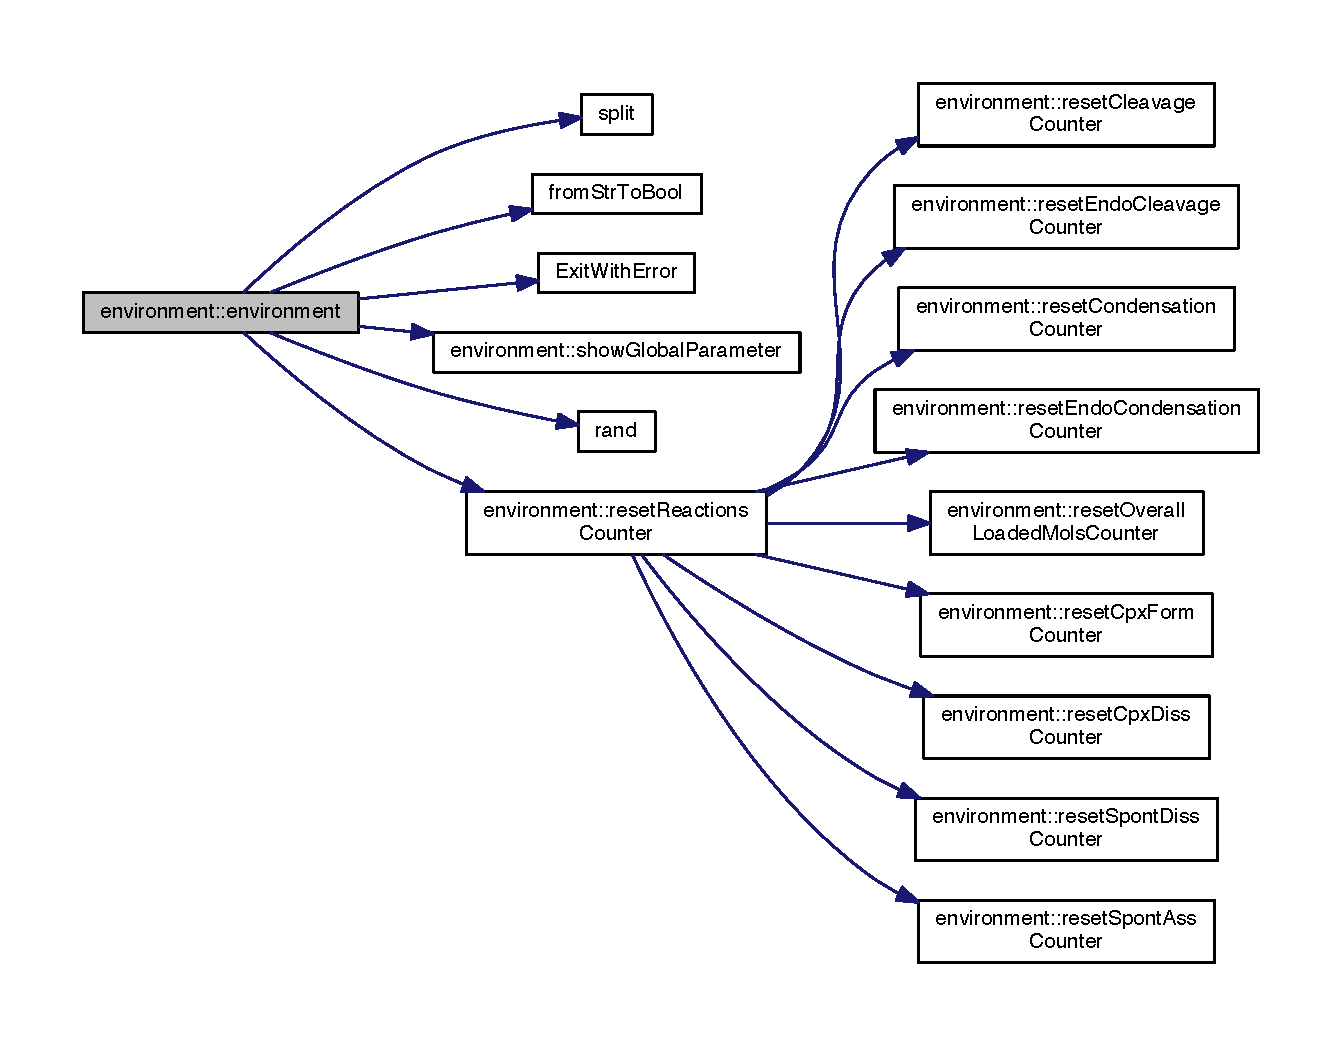
\includegraphics[width=350pt]{a00013_aa44bbabec52bf2d61a19685a30e68de1_cgraph}
\end{center}
\end{figure}


\hypertarget{a00013_ae323954bd5b674bf34d954c3f7b67629}{\index{environment@{environment}!````~environment@{$\sim$environment}}
\index{````~environment@{$\sim$environment}!environment@{environment}}
\subsubsection[{$\sim$environment}]{\setlength{\rightskip}{0pt plus 5cm}environment\+::$\sim$environment (
\begin{DoxyParamCaption}
{}
\end{DoxyParamCaption}
)\hspace{0.3cm}{\ttfamily [inline]}}}\label{a00013_ae323954bd5b674bf34d954c3f7b67629}


Definition at line 148 of file environment.\+h.

\hypertarget{a00013_aa44bbabec52bf2d61a19685a30e68de1}{\index{environment@{environment}!environment@{environment}}
\index{environment@{environment}!environment@{environment}}
\subsubsection[{environment}]{\setlength{\rightskip}{0pt plus 5cm}environment\+::environment (
\begin{DoxyParamCaption}
\item[{string}]{tmp\+Initial\+Path}
\end{DoxyParamCaption}
)}}\label{a00013_aa44bbabec52bf2d61a19685a30e68de1}
\hypertarget{a00013_ae323954bd5b674bf34d954c3f7b67629}{\index{environment@{environment}!````~environment@{$\sim$environment}}
\index{````~environment@{$\sim$environment}!environment@{environment}}
\subsubsection[{$\sim$environment}]{\setlength{\rightskip}{0pt plus 5cm}environment\+::$\sim$environment (
\begin{DoxyParamCaption}
{}
\end{DoxyParamCaption}
)\hspace{0.3cm}{\ttfamily [inline]}}}\label{a00013_ae323954bd5b674bf34d954c3f7b67629}


Definition at line 160 of file environment.\+h.



\subsection{Member Function Documentation}
\hypertarget{a00013_a7981c34d16c0b1e9e6ca3ea69aa3a8a3}{\index{environment@{environment}!add\+Charge\+Mol\+To\+List@{add\+Charge\+Mol\+To\+List}}
\index{add\+Charge\+Mol\+To\+List@{add\+Charge\+Mol\+To\+List}!environment@{environment}}
\subsubsection[{add\+Charge\+Mol\+To\+List}]{\setlength{\rightskip}{0pt plus 5cm}bool environment\+::add\+Charge\+Mol\+To\+List (
\begin{DoxyParamCaption}
\item[{{\bf acs\+\_\+int}}]{tmp\+Species\+I\+D}
\end{DoxyParamCaption}
)}}\label{a00013_a7981c34d16c0b1e9e6ca3ea69aa3a8a3}
Perform vector uncharged\+I\+Dlist update adding a new charge molecule vector uncharged\+I\+Dlist and cum\+Uncharged\+Amount\+List are involved \begin{DoxyVersion}{Version}
1.\+0 
\end{DoxyVersion}
\begin{DoxyDate}{Date}
2010-\/10-\/10 
\end{DoxyDate}

\begin{DoxyParams}{Parameters}
{\em acs\+\_\+int} & tmp\+Species\+I\+D Specie to charge \\
\hline
\end{DoxyParams}


Definition at line 4295 of file environment.\+cpp.



Here is the call graph for this function\+:\nopagebreak
\begin{figure}[H]
\begin{center}
\leavevmode
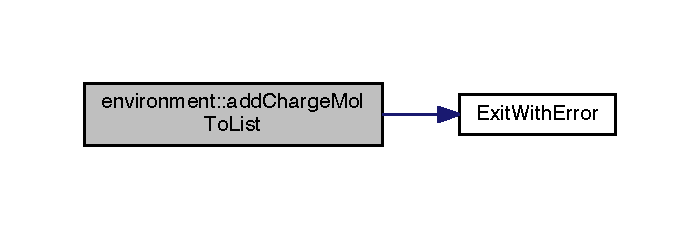
\includegraphics[width=336pt]{a00013_a7981c34d16c0b1e9e6ca3ea69aa3a8a3_cgraph}
\end{center}
\end{figure}


\hypertarget{a00013_a7981c34d16c0b1e9e6ca3ea69aa3a8a3}{\index{environment@{environment}!add\+Charge\+Mol\+To\+List@{add\+Charge\+Mol\+To\+List}}
\index{add\+Charge\+Mol\+To\+List@{add\+Charge\+Mol\+To\+List}!environment@{environment}}
\subsubsection[{add\+Charge\+Mol\+To\+List}]{\setlength{\rightskip}{0pt plus 5cm}bool environment\+::add\+Charge\+Mol\+To\+List (
\begin{DoxyParamCaption}
\item[{{\bf acs\+\_\+int}}]{tmp\+Species\+I\+D}
\end{DoxyParamCaption}
)}}\label{a00013_a7981c34d16c0b1e9e6ca3ea69aa3a8a3}
\hypertarget{a00013_a0156a2d7219396e58a930731966b0c66}{\index{environment@{environment}!change\+Volume@{change\+Volume}}
\index{change\+Volume@{change\+Volume}!environment@{environment}}
\subsubsection[{change\+Volume}]{\setlength{\rightskip}{0pt plus 5cm}void environment\+::change\+Volume (
\begin{DoxyParamCaption}
\item[{{\bf acs\+\_\+int}}]{tmp\+Time\+Since\+Last\+Reaction}
\end{DoxyParamCaption}
)}}\label{a00013_a0156a2d7219396e58a930731966b0c66}
Change volume function  1.\+0 \begin{DoxyDate}{Date}
2013/07/17 
\end{DoxyDate}
\begin{DoxyAuthor}{Author}
Alessandro Filisetti 
\end{DoxyAuthor}


Definition at line 6139 of file environment.\+cpp.



Here is the caller graph for this function\+:\nopagebreak
\begin{figure}[H]
\begin{center}
\leavevmode
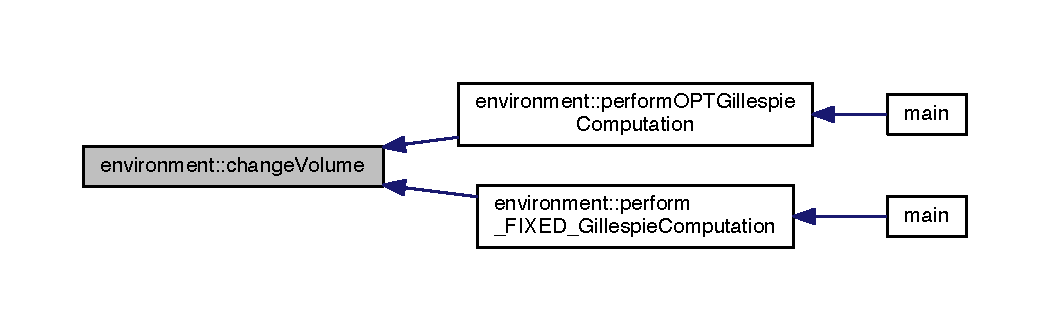
\includegraphics[width=350pt]{a00013_a0156a2d7219396e58a930731966b0c66_icgraph}
\end{center}
\end{figure}


\hypertarget{a00013_a0156a2d7219396e58a930731966b0c66}{\index{environment@{environment}!change\+Volume@{change\+Volume}}
\index{change\+Volume@{change\+Volume}!environment@{environment}}
\subsubsection[{change\+Volume}]{\setlength{\rightskip}{0pt plus 5cm}void environment\+::change\+Volume (
\begin{DoxyParamCaption}
\item[{{\bf acs\+\_\+int}}]{tmp\+Time\+Since\+Last\+Reaction}
\end{DoxyParamCaption}
)}}\label{a00013_a0156a2d7219396e58a930731966b0c66}
\hypertarget{a00013_ad3ebcd7ab1c9ba1a0f65b264b97adf33}{\index{environment@{environment}!check\+Availability@{check\+Availability}}
\index{check\+Availability@{check\+Availability}!environment@{environment}}
\subsubsection[{check\+Availability}]{\setlength{\rightskip}{0pt plus 5cm}bool environment\+::check\+Availability (
\begin{DoxyParamCaption}
\item[{{\bf acs\+\_\+long\+Int}}]{tmp\+M\+I, }
\item[{{\bf acs\+\_\+long\+Int}}]{tmp\+M\+I\+I, }
\item[{{\bf acs\+\_\+long\+Int}}]{tmp\+Q\+I, }
\item[{{\bf acs\+\_\+long\+Int}}]{tmp\+Q\+I\+I}
\end{DoxyParamCaption}
)}}\label{a00013_ad3ebcd7ab1c9ba1a0f65b264b97adf33}
Return T\+R\+U\+E if there are sufficient molecules for the reaction. It is used for the reaction in which catalyst and substrate are the same molecules \begin{DoxyVersion}{Version}
1.\+0 
\end{DoxyVersion}
\begin{DoxyDate}{Date}
2011.\+07.\+25 
\end{DoxyDate}

\begin{DoxyParams}{Parameters}
{\em tmp\+M\+I} & \\
\hline
{\em tmp\+M\+I\+I} & \\
\hline
{\em tmp\+Q\+I} & \\
\hline
{\em tmp\+Q\+I\+I} & \\
\hline
\end{DoxyParams}


Definition at line 2635 of file environment.\+cpp.



Here is the call graph for this function\+:\nopagebreak
\begin{figure}[H]
\begin{center}
\leavevmode
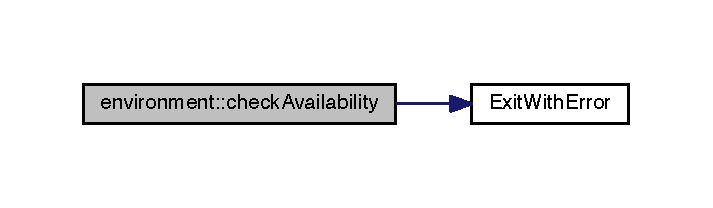
\includegraphics[width=342pt]{a00013_ad3ebcd7ab1c9ba1a0f65b264b97adf33_cgraph}
\end{center}
\end{figure}




Here is the caller graph for this function\+:\nopagebreak
\begin{figure}[H]
\begin{center}
\leavevmode
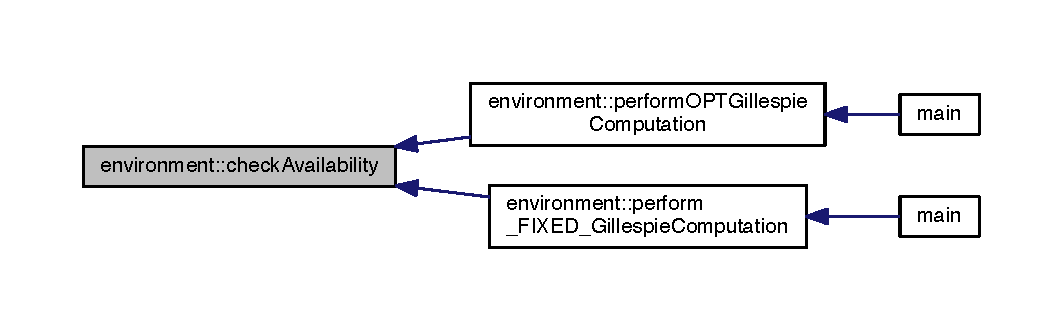
\includegraphics[width=350pt]{a00013_ad3ebcd7ab1c9ba1a0f65b264b97adf33_icgraph}
\end{center}
\end{figure}


\hypertarget{a00013_ad3ebcd7ab1c9ba1a0f65b264b97adf33}{\index{environment@{environment}!check\+Availability@{check\+Availability}}
\index{check\+Availability@{check\+Availability}!environment@{environment}}
\subsubsection[{check\+Availability}]{\setlength{\rightskip}{0pt plus 5cm}bool environment\+::check\+Availability (
\begin{DoxyParamCaption}
\item[{{\bf acs\+\_\+long\+Int}}]{tmp\+M\+I, }
\item[{{\bf acs\+\_\+long\+Int}}]{tmp\+M\+I\+I, }
\item[{{\bf acs\+\_\+long\+Int}}]{tmp\+Q\+I, }
\item[{{\bf acs\+\_\+long\+Int}}]{tmp\+Q\+I\+I}
\end{DoxyParamCaption}
)}}\label{a00013_ad3ebcd7ab1c9ba1a0f65b264b97adf33}
\hypertarget{a00013_abdafaeba15b5d32fd35569869c6244d5}{\index{environment@{environment}!check\+If\+Only\+Mutual\+Catalysis@{check\+If\+Only\+Mutual\+Catalysis}}
\index{check\+If\+Only\+Mutual\+Catalysis@{check\+If\+Only\+Mutual\+Catalysis}!environment@{environment}}
\subsubsection[{check\+If\+Only\+Mutual\+Catalysis}]{\setlength{\rightskip}{0pt plus 5cm}bool environment\+::check\+If\+Only\+Mutual\+Catalysis (
\begin{DoxyParamCaption}
\item[{{\bf acs\+\_\+int}}]{tmp\+Cat, }
\item[{{\bf acs\+\_\+int}}]{tmp\+Candidate\+Product}
\end{DoxyParamCaption}
)}}\label{a00013_abdafaeba15b5d32fd35569869c6244d5}
This function return false if the tmp\+Candidate\+Product is a catalyst of tmp\+Cat \begin{DoxyVersion}{Version}
1.\+0 -\/ last update 2009/10/08 -\/ build 009 
\end{DoxyVersion}


Definition at line 1965 of file environment.\+cpp.



Here is the call graph for this function\+:\nopagebreak
\begin{figure}[H]
\begin{center}
\leavevmode
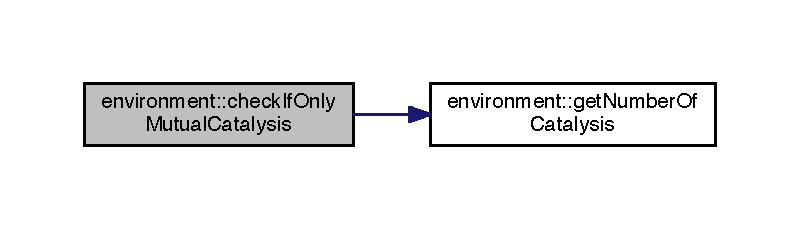
\includegraphics[width=350pt]{a00013_abdafaeba15b5d32fd35569869c6244d5_cgraph}
\end{center}
\end{figure}


\hypertarget{a00013_abdafaeba15b5d32fd35569869c6244d5}{\index{environment@{environment}!check\+If\+Only\+Mutual\+Catalysis@{check\+If\+Only\+Mutual\+Catalysis}}
\index{check\+If\+Only\+Mutual\+Catalysis@{check\+If\+Only\+Mutual\+Catalysis}!environment@{environment}}
\subsubsection[{check\+If\+Only\+Mutual\+Catalysis}]{\setlength{\rightskip}{0pt plus 5cm}bool environment\+::check\+If\+Only\+Mutual\+Catalysis (
\begin{DoxyParamCaption}
\item[{{\bf acs\+\_\+int}}]{tmp\+Cat, }
\item[{{\bf acs\+\_\+int}}]{tmp\+Candidate\+Product}
\end{DoxyParamCaption}
)}}\label{a00013_abdafaeba15b5d32fd35569869c6244d5}
\hypertarget{a00013_ac4c90b07b8e75ea03e2ced0ea644a69f}{\index{environment@{environment}!check\+If\+The\+Reaction\+Is\+Already\+Catalyzed\+By\+This\+Species@{check\+If\+The\+Reaction\+Is\+Already\+Catalyzed\+By\+This\+Species}}
\index{check\+If\+The\+Reaction\+Is\+Already\+Catalyzed\+By\+This\+Species@{check\+If\+The\+Reaction\+Is\+Already\+Catalyzed\+By\+This\+Species}!environment@{environment}}
\subsubsection[{check\+If\+The\+Reaction\+Is\+Already\+Catalyzed\+By\+This\+Species}]{\setlength{\rightskip}{0pt plus 5cm}bool environment\+::check\+If\+The\+Reaction\+Is\+Already\+Catalyzed\+By\+This\+Species (
\begin{DoxyParamCaption}
\item[{{\bf acs\+\_\+long\+Int}}]{tmp\+S\+Pecies\+I\+D, }
\item[{{\bf acs\+\_\+long\+Int}}]{tmp\+Id\+Reaction}
\end{DoxyParamCaption}
)}}\label{a00013_ac4c90b07b8e75ea03e2ced0ea644a69f}
If the reaction is not new this function checks if the reactions has been already catalysed by this species \begin{DoxyVersion}{Version}
1.\+0 
\end{DoxyVersion}

\begin{DoxyParams}{Parameters}
{\em acs\+\_\+int} & tmp\+S\+Pecies\+I\+D catalyst I\+D \\
\hline
{\em tmp\+Id\+Reaction} & reaction I\+D \\
\hline
\end{DoxyParams}


Definition at line 1937 of file environment.\+cpp.



Here is the call graph for this function\+:\nopagebreak
\begin{figure}[H]
\begin{center}
\leavevmode
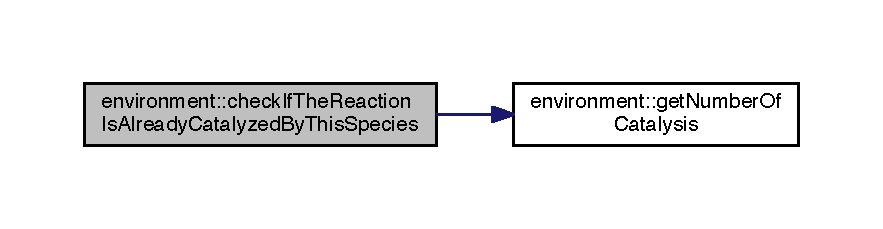
\includegraphics[width=350pt]{a00013_ac4c90b07b8e75ea03e2ced0ea644a69f_cgraph}
\end{center}
\end{figure}




Here is the caller graph for this function\+:\nopagebreak
\begin{figure}[H]
\begin{center}
\leavevmode
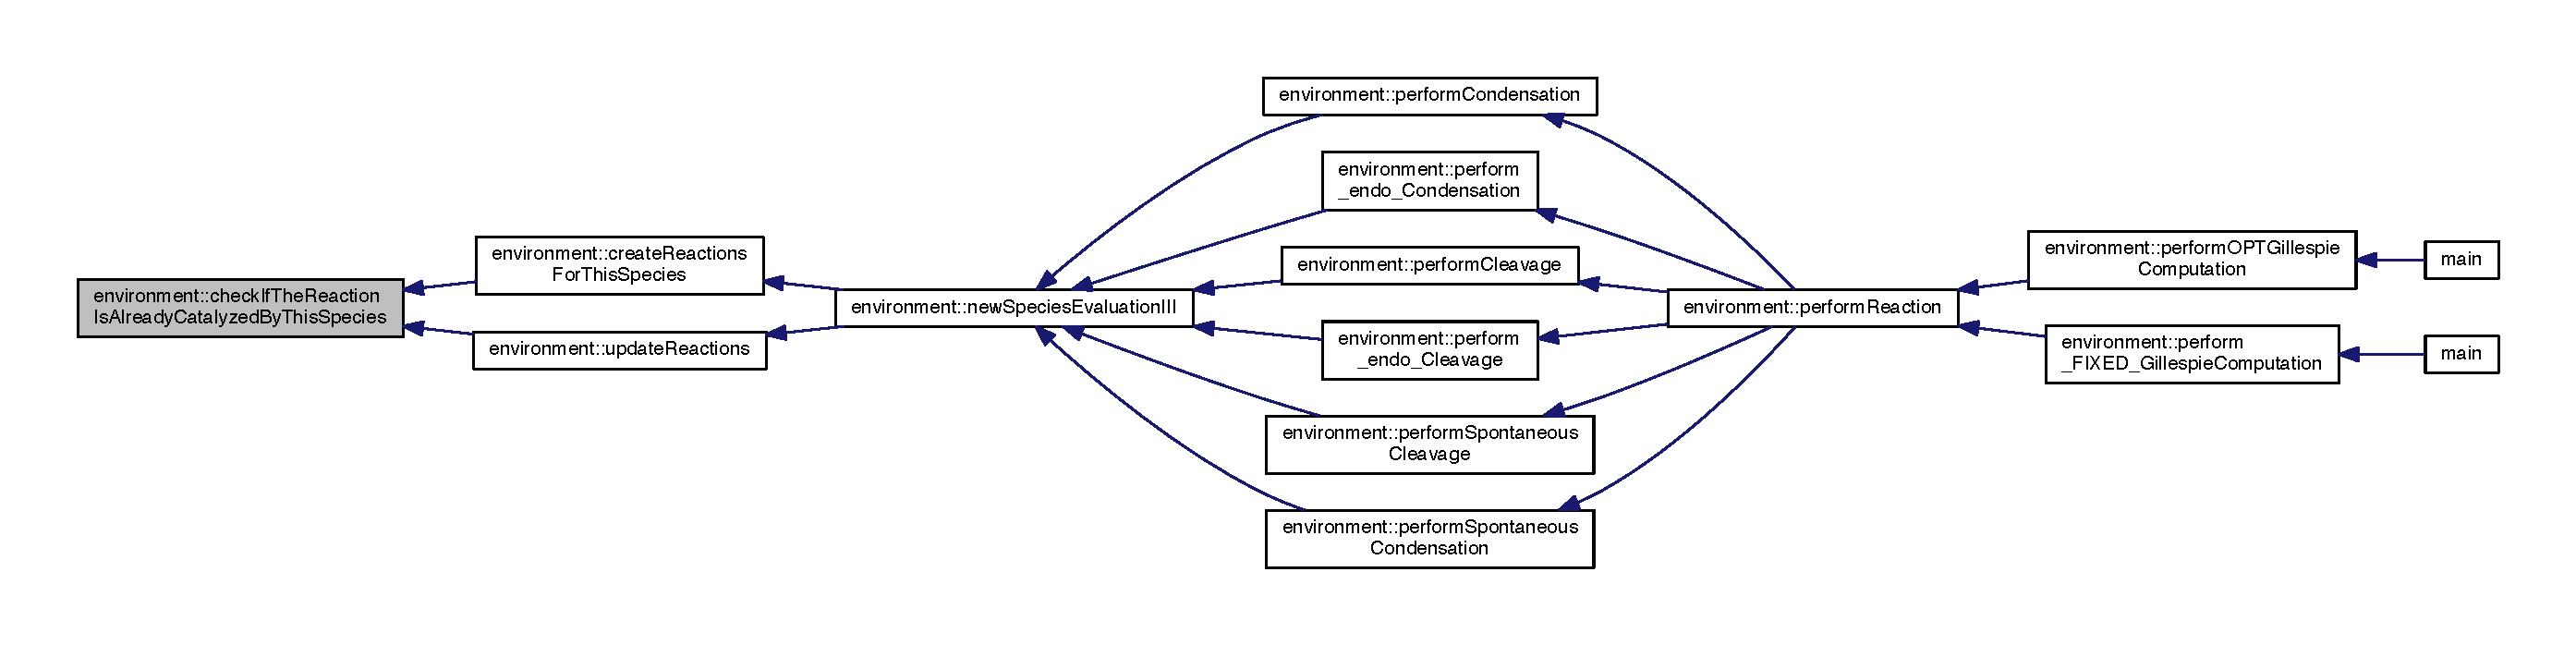
\includegraphics[width=350pt]{a00013_ac4c90b07b8e75ea03e2ced0ea644a69f_icgraph}
\end{center}
\end{figure}


\hypertarget{a00013_ac4c90b07b8e75ea03e2ced0ea644a69f}{\index{environment@{environment}!check\+If\+The\+Reaction\+Is\+Already\+Catalyzed\+By\+This\+Species@{check\+If\+The\+Reaction\+Is\+Already\+Catalyzed\+By\+This\+Species}}
\index{check\+If\+The\+Reaction\+Is\+Already\+Catalyzed\+By\+This\+Species@{check\+If\+The\+Reaction\+Is\+Already\+Catalyzed\+By\+This\+Species}!environment@{environment}}
\subsubsection[{check\+If\+The\+Reaction\+Is\+Already\+Catalyzed\+By\+This\+Species}]{\setlength{\rightskip}{0pt plus 5cm}bool environment\+::check\+If\+The\+Reaction\+Is\+Already\+Catalyzed\+By\+This\+Species (
\begin{DoxyParamCaption}
\item[{{\bf acs\+\_\+long\+Int}}]{tmp\+S\+Pecies\+I\+D, }
\item[{{\bf acs\+\_\+long\+Int}}]{tmp\+Id\+Reaction}
\end{DoxyParamCaption}
)}}\label{a00013_ac4c90b07b8e75ea03e2ced0ea644a69f}
\hypertarget{a00013_aa860227725dbe5b0251a25f440773161}{\index{environment@{environment}!clear\+All\+Structures@{clear\+All\+Structures}}
\index{clear\+All\+Structures@{clear\+All\+Structures}!environment@{environment}}
\subsubsection[{clear\+All\+Structures}]{\setlength{\rightskip}{0pt plus 5cm}void environment\+::clear\+All\+Structures (
\begin{DoxyParamCaption}
{}
\end{DoxyParamCaption}
)}}\label{a00013_aa860227725dbe5b0251a25f440773161}
Clear all structures after each simulation \begin{DoxyVersion}{Version}
1.\+0 
\end{DoxyVersion}


Definition at line 6387 of file environment.\+cpp.



Here is the call graph for this function\+:\nopagebreak
\begin{figure}[H]
\begin{center}
\leavevmode
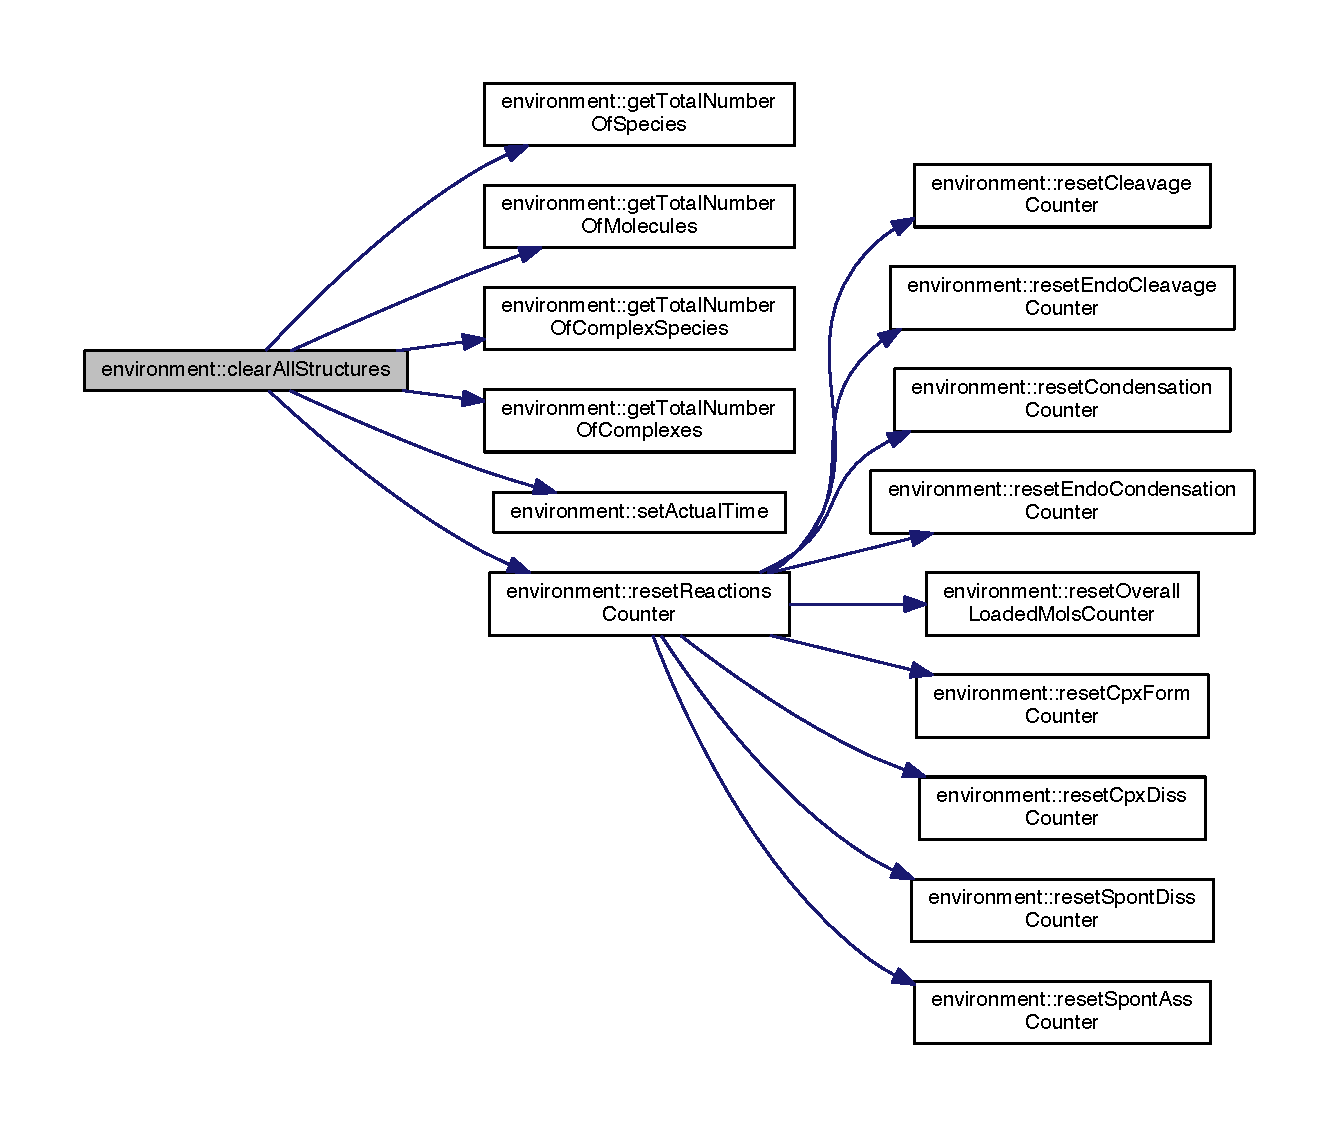
\includegraphics[width=350pt]{a00013_aa860227725dbe5b0251a25f440773161_cgraph}
\end{center}
\end{figure}




Here is the caller graph for this function\+:\nopagebreak
\begin{figure}[H]
\begin{center}
\leavevmode
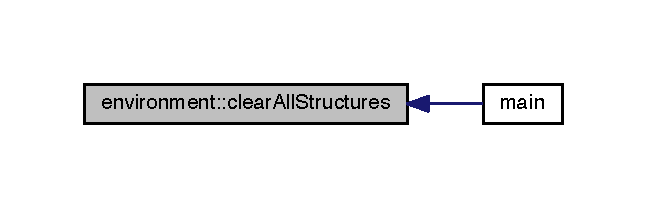
\includegraphics[width=310pt]{a00013_aa860227725dbe5b0251a25f440773161_icgraph}
\end{center}
\end{figure}


\hypertarget{a00013_aa860227725dbe5b0251a25f440773161}{\index{environment@{environment}!clear\+All\+Structures@{clear\+All\+Structures}}
\index{clear\+All\+Structures@{clear\+All\+Structures}!environment@{environment}}
\subsubsection[{clear\+All\+Structures}]{\setlength{\rightskip}{0pt plus 5cm}void environment\+::clear\+All\+Structures (
\begin{DoxyParamCaption}
{}
\end{DoxyParamCaption}
)}}\label{a00013_aa860227725dbe5b0251a25f440773161}
\hypertarget{a00013_aa33d7b81db9632c8ba1f9ce3f362df8e}{\index{environment@{environment}!clear\+Gil\+Scores@{clear\+Gil\+Scores}}
\index{clear\+Gil\+Scores@{clear\+Gil\+Scores}!environment@{environment}}
\subsubsection[{clear\+Gil\+Scores}]{\setlength{\rightskip}{0pt plus 5cm}void environment\+::clear\+Gil\+Scores (
\begin{DoxyParamCaption}
{}
\end{DoxyParamCaption}
)}}\label{a00013_aa33d7b81db9632c8ba1f9ce3f362df8e}
Clear gillespie structure and species' events lists after each generation \begin{DoxyVersion}{Version}
1.\+0 
\end{DoxyVersion}


Definition at line 7770 of file environment.\+cpp.



Here is the caller graph for this function\+:\nopagebreak
\begin{figure}[H]
\begin{center}
\leavevmode
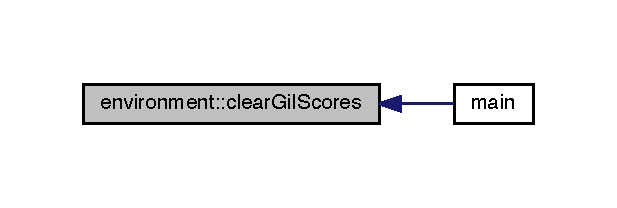
\includegraphics[width=296pt]{a00013_aa33d7b81db9632c8ba1f9ce3f362df8e_icgraph}
\end{center}
\end{figure}


\hypertarget{a00013_a5ee6b203f077de1467aa72042814db7d}{\index{environment@{environment}!complex\+Evaluation@{complex\+Evaluation}}
\index{complex\+Evaluation@{complex\+Evaluation}!environment@{environment}}
\subsubsection[{complex\+Evaluation}]{\setlength{\rightskip}{0pt plus 5cm}bool environment\+::complex\+Evaluation (
\begin{DoxyParamCaption}
\item[{string}]{tmp\+Complex, }
\item[{{\bf M\+T\+Rand} \&}]{tmp\+\_\+\+\_\+\+\_\+\+Rnd\+Double\+Gen, }
\item[{{\bf acs\+\_\+int}}]{tmp\+Cutting\+Pnt, }
\item[{{\bf acs\+\_\+long\+Int}}]{tmp\+Catalyst\+\_\+\+I\+D, }
\item[{{\bf acs\+\_\+long\+Int}}]{tmp\+Substrate\+\_\+\+I\+D, }
\item[{{\bf acs\+\_\+long\+Int}}]{tmp\+Cat\+I\+D, }
\item[{{\bf acs\+\_\+long\+Int}}]{tmp\+Sec\+Sub\+\_\+\+I\+D, }
\item[{bool}]{tmp\+Cpx\+Type}
\end{DoxyParamCaption}
)}}\label{a00013_a5ee6b203f077de1467aa72042814db7d}
Complex evaluation \begin{DoxyVersion}{Version}
1.\+1 
\end{DoxyVersion}
\begin{DoxyDate}{Date}
2010-\/06-\/04 
\end{DoxyDate}

\begin{DoxyParams}{Parameters}
{\em string} & tmp\+New\+Species New species sequence to evaluate \\
\hline
{\em M\+T\+Rand\&} & tmp\+\_\+\+\_\+\+\_\+\+Rnd\+Double\+Gen random number generator \\
\hline
{\em tmp\+Cutting\+Pnt} & Complex cutting point \\
\hline
{\em tmp\+Catalyst\+\_\+\+I\+D} & catalyst I\+D \\
\hline
{\em tmp\+Substrate\+\_\+\+I\+D} & substrate I\+D \\
\hline
{\em tmp\+\_\+catalysis\+I\+D} & catalysis I\+D \\
\hline
{\em tmp\+Cpx\+Type} & E\+N\+D\+O\+E\+R\+G\+O\+N\+I\+C or E\+S\+O\+E\+R\+G\+O\+N\+I\+C \\
\hline
\end{DoxyParams}


Definition at line 6007 of file environment.\+cpp.



Here is the call graph for this function\+:\nopagebreak
\begin{figure}[H]
\begin{center}
\leavevmode
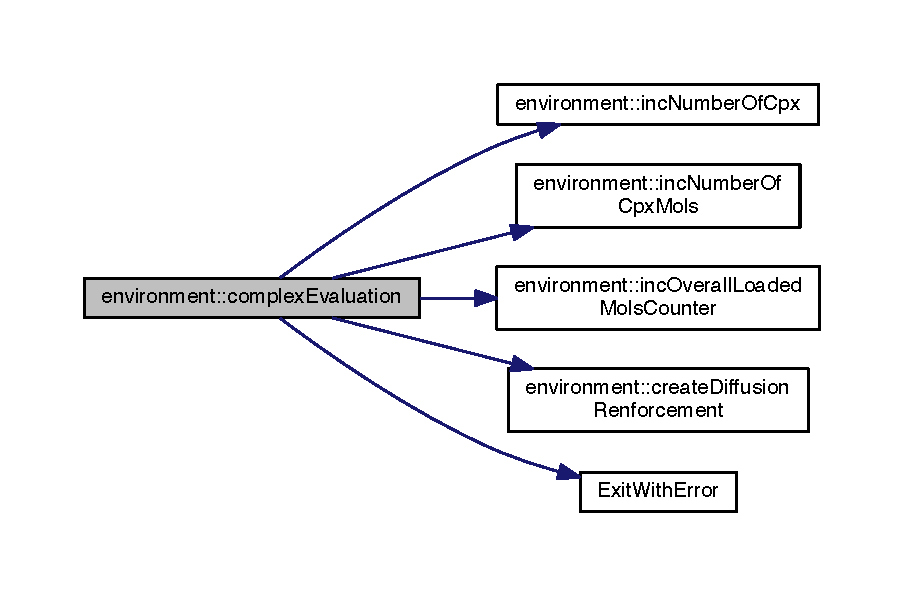
\includegraphics[width=350pt]{a00013_a5ee6b203f077de1467aa72042814db7d_cgraph}
\end{center}
\end{figure}




Here is the caller graph for this function\+:\nopagebreak
\begin{figure}[H]
\begin{center}
\leavevmode
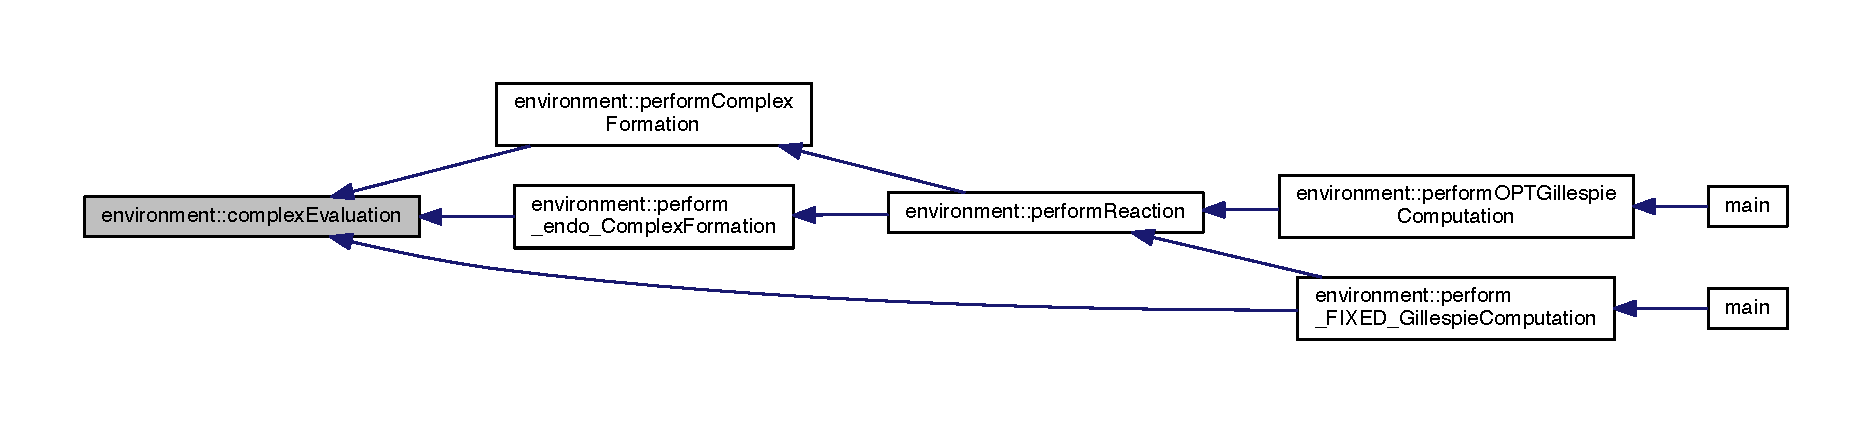
\includegraphics[width=350pt]{a00013_a5ee6b203f077de1467aa72042814db7d_icgraph}
\end{center}
\end{figure}


\hypertarget{a00013_a5ee6b203f077de1467aa72042814db7d}{\index{environment@{environment}!complex\+Evaluation@{complex\+Evaluation}}
\index{complex\+Evaluation@{complex\+Evaluation}!environment@{environment}}
\subsubsection[{complex\+Evaluation}]{\setlength{\rightskip}{0pt plus 5cm}bool environment\+::complex\+Evaluation (
\begin{DoxyParamCaption}
\item[{string}]{tmp\+Complex, }
\item[{{\bf M\+T\+Rand} \&}]{tmp\+\_\+\+\_\+\+\_\+\+Rnd\+Double\+Gen, }
\item[{{\bf acs\+\_\+int}}]{tmp\+Cutting\+Pnt, }
\item[{{\bf acs\+\_\+long\+Int}}]{tmp\+Catalyst\+\_\+\+I\+D, }
\item[{{\bf acs\+\_\+long\+Int}}]{tmp\+Cat\+I\+D, }
\item[{{\bf acs\+\_\+long\+Int}}]{tmp\+Substrate\+\_\+\+I\+D, }
\item[{{\bf acs\+\_\+long\+Int}}]{tmp\+Sec\+Sub\+\_\+\+I\+D, }
\item[{bool}]{tmp\+Cpx\+Type}
\end{DoxyParamCaption}
)}}\label{a00013_a5ee6b203f077de1467aa72042814db7d}
\hypertarget{a00013_ae1270b9c235dd6b28413075197dba8e0}{\index{environment@{environment}!compute\+Singl\+Gil\+Score@{compute\+Singl\+Gil\+Score}}
\index{compute\+Singl\+Gil\+Score@{compute\+Singl\+Gil\+Score}!environment@{environment}}
\subsubsection[{compute\+Singl\+Gil\+Score}]{\setlength{\rightskip}{0pt plus 5cm}{\bf acs\+\_\+double} environment\+::compute\+Singl\+Gil\+Score (
\begin{DoxyParamCaption}
\item[{{\bf acs\+\_\+long\+Int}}]{tmp\+Amount\+I, }
\item[{{\bf acs\+\_\+double}}]{tmp\+Dif\+I, }
\item[{{\bf acs\+\_\+int}}]{tmp\+Sol\+I, }
\item[{{\bf acs\+\_\+long\+Int}}]{tmp\+Amount\+I\+I, }
\item[{{\bf acs\+\_\+double}}]{tmp\+Dif\+I\+I, }
\item[{{\bf acs\+\_\+int}}]{tmp\+Sol\+I\+I, }
\item[{{\bf acs\+\_\+double}}]{tmp\+K, }
\item[{bool}]{tmp\+Same\+Mol}
\end{DoxyParamCaption}
)}}\label{a00013_ae1270b9c235dd6b28413075197dba8e0}
Compute a single gillespie score according to the amount and peoprieties of the species involved \begin{DoxyVersion}{Version}
1.\+0 
\end{DoxyVersion}
\begin{DoxyDate}{Date}
20110214
\end{DoxyDate}
Compute a single gillespie score according to the amount and properties of the species involved \begin{DoxyVersion}{Version}
1.\+0 
\end{DoxyVersion}
\begin{DoxyDate}{Date}
20110214 
\end{DoxyDate}


Definition at line 3270 of file environment.\+cpp.



Here is the caller graph for this function\+:\nopagebreak
\begin{figure}[H]
\begin{center}
\leavevmode
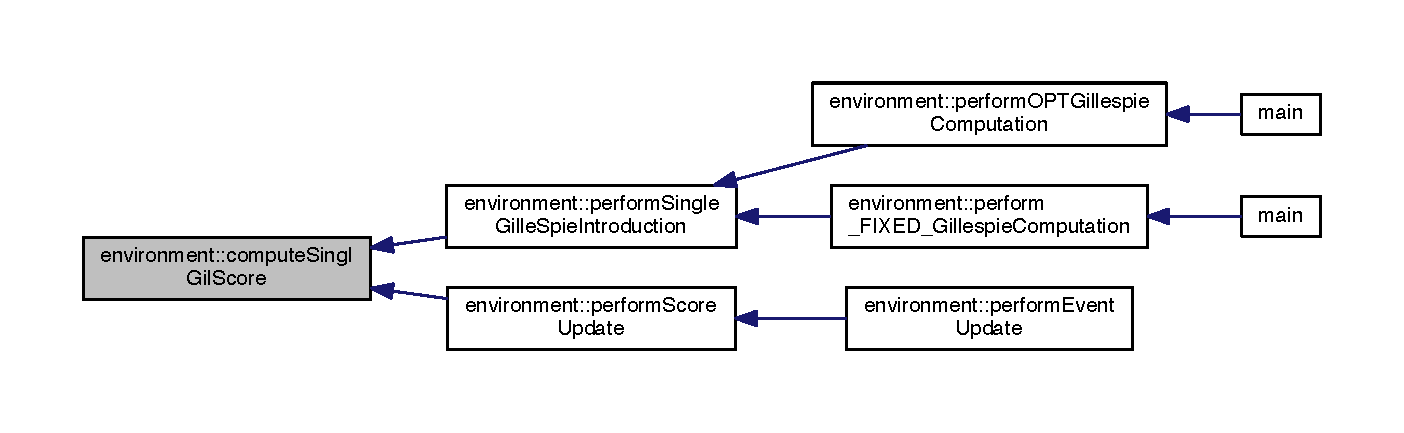
\includegraphics[width=350pt]{a00013_ae1270b9c235dd6b28413075197dba8e0_icgraph}
\end{center}
\end{figure}


\hypertarget{a00013_ae1270b9c235dd6b28413075197dba8e0}{\index{environment@{environment}!compute\+Singl\+Gil\+Score@{compute\+Singl\+Gil\+Score}}
\index{compute\+Singl\+Gil\+Score@{compute\+Singl\+Gil\+Score}!environment@{environment}}
\subsubsection[{compute\+Singl\+Gil\+Score}]{\setlength{\rightskip}{0pt plus 5cm}{\bf acs\+\_\+double} environment\+::compute\+Singl\+Gil\+Score (
\begin{DoxyParamCaption}
\item[{{\bf acs\+\_\+long\+Int}}]{tmp\+Amount\+I, }
\item[{{\bf acs\+\_\+double}}]{tmp\+Dif\+I, }
\item[{{\bf acs\+\_\+int}}]{tmp\+Sol\+I, }
\item[{{\bf acs\+\_\+long\+Int}}]{tmp\+Amount\+I\+I, }
\item[{{\bf acs\+\_\+double}}]{tmp\+Dif\+I\+I, }
\item[{{\bf acs\+\_\+int}}]{tmp\+Sol\+I\+I, }
\item[{{\bf acs\+\_\+double}}]{tmp\+K, }
\item[{bool}]{tmp\+Same\+Mol}
\end{DoxyParamCaption}
)}}\label{a00013_ae1270b9c235dd6b28413075197dba8e0}
\hypertarget{a00013_a0fd3cb062d35d2f6dd8961e95dd477b7}{\index{environment@{environment}!compute\+Sng\+Species\+Rcts\+Number@{compute\+Sng\+Species\+Rcts\+Number}}
\index{compute\+Sng\+Species\+Rcts\+Number@{compute\+Sng\+Species\+Rcts\+Number}!environment@{environment}}
\subsubsection[{compute\+Sng\+Species\+Rcts\+Number}]{\setlength{\rightskip}{0pt plus 5cm}{\bf acs\+\_\+int} environment\+::compute\+Sng\+Species\+Rcts\+Number (
\begin{DoxyParamCaption}
\item[{{\bf acs\+\_\+long\+Int}}]{tmp\+Total\+Number\+Of\+Reactions, }
\item[{{\bf M\+T\+Rand} \&}]{tmp\+Rnd\+Double\+Gen}
\end{DoxyParamCaption}
)}}\label{a00013_a0fd3cb062d35d2f6dd8961e95dd477b7}
Initial molecule population creation. If the number of species stored in the configuration file is grater than the possible number of species according to the alphabet and maximum length all species up to the M\+A\+X length will be created \begin{DoxyVersion}{Version}
1.\+0 
\end{DoxyVersion}

\begin{DoxyParams}{Parameters}
{\em M\+T\+Rand\&} & tmp\+Rnd\+Double\+Gen initial layer initialization \\
\hline
\end{DoxyParams}
\begin{DoxyVersion}{Version}
1.\+0 
\end{DoxyVersion}

\begin{DoxyParams}{Parameters}
{\em M\+T\+Rand\&} & tmp\+Rnd\+Double\+Gen Compute number of reaction catalysd by a catalyst according to the total number of reactions and reactions probabilities \\
\hline
\end{DoxyParams}
\begin{DoxyVersion}{Version}
1.\+0 
\end{DoxyVersion}

\begin{DoxyParams}{Parameters}
{\em acs\+\_\+int} & tmp\+Total\+Number\+Of\+Reactions Total number of conceivable reactions \\
\hline
{\em acs\+\_\+double} & tmp\+Rcts\+Prob reaction probability \\
\hline
\end{DoxyParams}


Definition at line 481 of file environment.\+cpp.



Here is the call graph for this function\+:\nopagebreak
\begin{figure}[H]
\begin{center}
\leavevmode
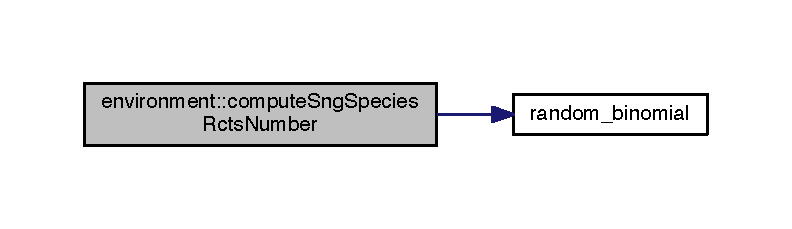
\includegraphics[width=350pt]{a00013_a0fd3cb062d35d2f6dd8961e95dd477b7_cgraph}
\end{center}
\end{figure}




Here is the caller graph for this function\+:\nopagebreak
\begin{figure}[H]
\begin{center}
\leavevmode
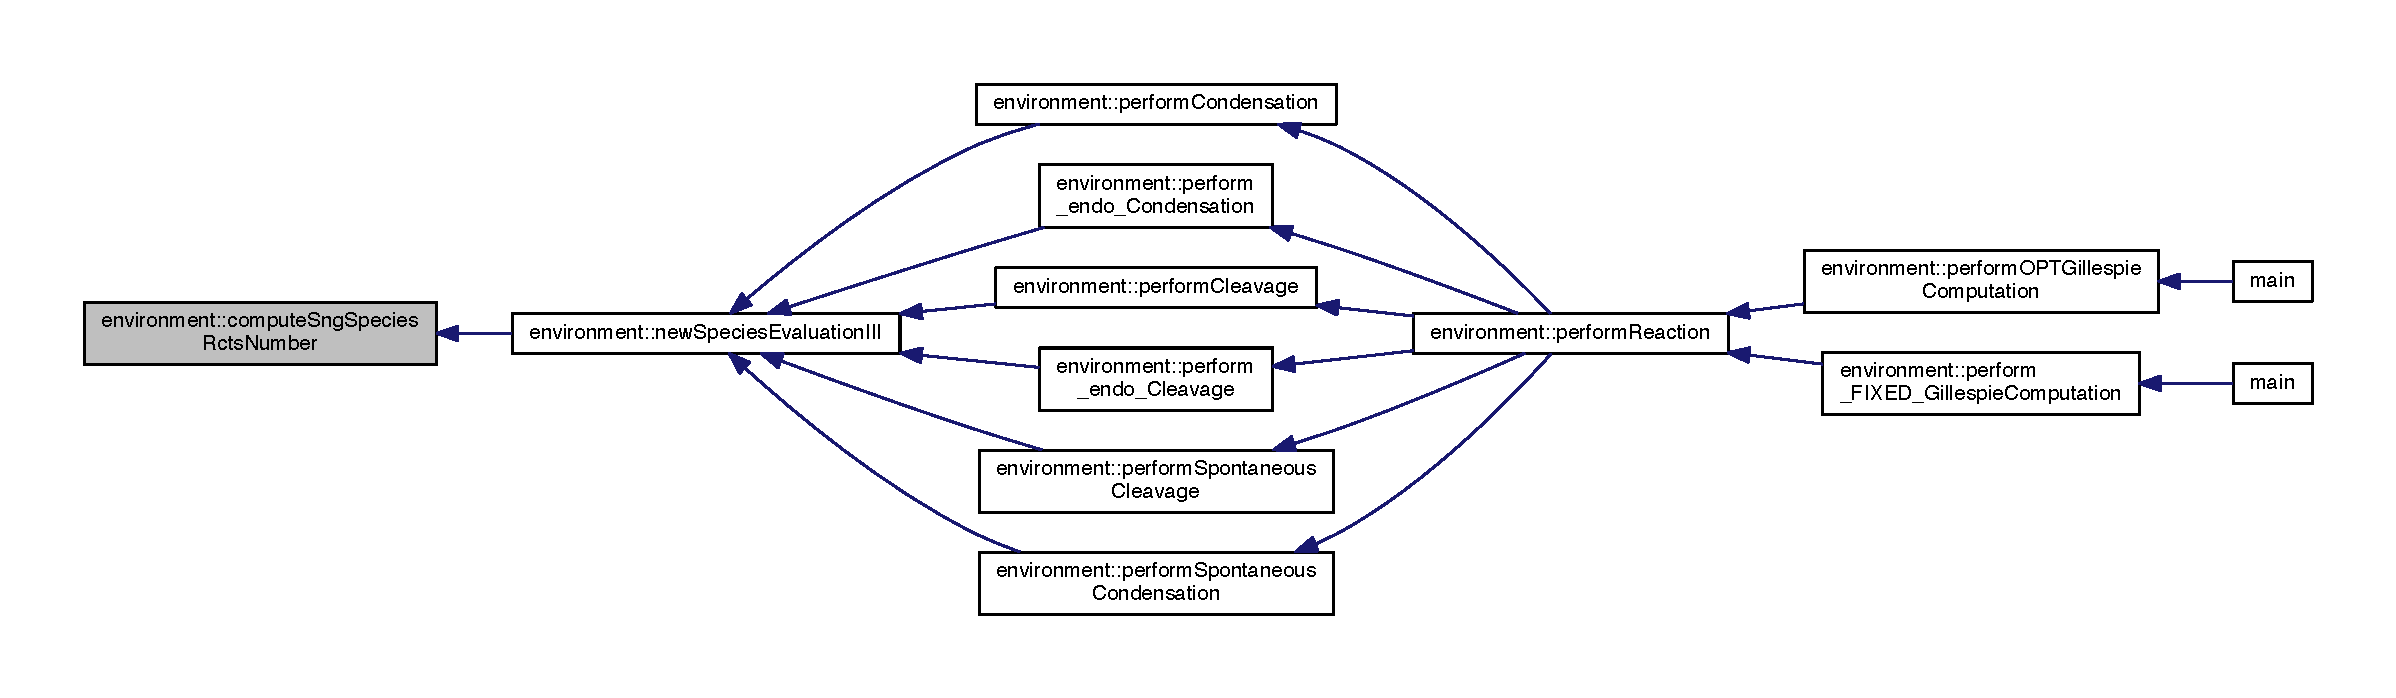
\includegraphics[width=350pt]{a00013_a0fd3cb062d35d2f6dd8961e95dd477b7_icgraph}
\end{center}
\end{figure}


\hypertarget{a00013_a0fd3cb062d35d2f6dd8961e95dd477b7}{\index{environment@{environment}!compute\+Sng\+Species\+Rcts\+Number@{compute\+Sng\+Species\+Rcts\+Number}}
\index{compute\+Sng\+Species\+Rcts\+Number@{compute\+Sng\+Species\+Rcts\+Number}!environment@{environment}}
\subsubsection[{compute\+Sng\+Species\+Rcts\+Number}]{\setlength{\rightskip}{0pt plus 5cm}{\bf acs\+\_\+int} environment\+::compute\+Sng\+Species\+Rcts\+Number (
\begin{DoxyParamCaption}
\item[{{\bf acs\+\_\+long\+Int}}]{tmp\+Total\+Number\+Of\+Reactions, }
\item[{{\bf M\+T\+Rand} \&}]{tmp\+Rnd\+Double\+Gen}
\end{DoxyParamCaption}
)}}\label{a00013_a0fd3cb062d35d2f6dd8961e95dd477b7}
\hypertarget{a00013_a375fc2dc0afc38a8a3afbd016acc4983}{\index{environment@{environment}!copy\+Species\+Initial\+Concentration\+Zero@{copy\+Species\+Initial\+Concentration\+Zero}}
\index{copy\+Species\+Initial\+Concentration\+Zero@{copy\+Species\+Initial\+Concentration\+Zero}!environment@{environment}}
\subsubsection[{copy\+Species\+Initial\+Concentration\+Zero}]{\setlength{\rightskip}{0pt plus 5cm}void environment\+::copy\+Species\+Initial\+Concentration\+Zero (
\begin{DoxyParamCaption}
{}
\end{DoxyParamCaption}
)}}\label{a00013_a375fc2dc0afc38a8a3afbd016acc4983}
This function copy in the vector species\+Initial\+Concentration\+Zero, the species with initial concentration equal to 0 \begin{DoxyVersion}{Version}
1.\+0 
\end{DoxyVersion}
\begin{DoxyDate}{Date}
2014-\/05-\/13 
\end{DoxyDate}


Definition at line 6083 of file environment.\+cpp.



Here is the caller graph for this function\+:\nopagebreak
\begin{figure}[H]
\begin{center}
\leavevmode
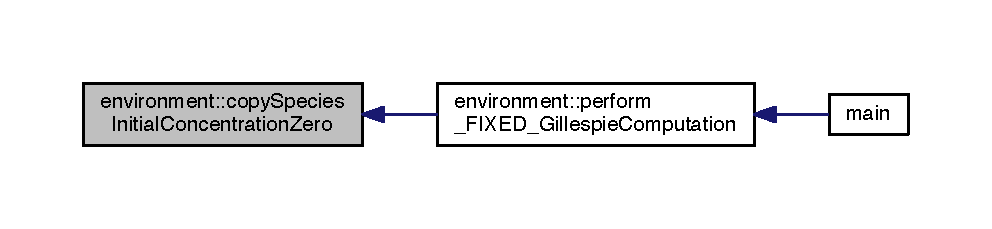
\includegraphics[width=350pt]{a00013_a375fc2dc0afc38a8a3afbd016acc4983_icgraph}
\end{center}
\end{figure}


\hypertarget{a00013_af795a4d1f04dfbfcbdf321e20e74f9c2}{\index{environment@{environment}!create\+Diffusion\+Renforcement@{create\+Diffusion\+Renforcement}}
\index{create\+Diffusion\+Renforcement@{create\+Diffusion\+Renforcement}!environment@{environment}}
\subsubsection[{create\+Diffusion\+Renforcement}]{\setlength{\rightskip}{0pt plus 5cm}{\bf acs\+\_\+double} environment\+::create\+Diffusion\+Renforcement (
\begin{DoxyParamCaption}
\item[{{\bf acs\+\_\+double}}]{tmp\+Diff\+Enh, }
\item[{{\bf acs\+\_\+int}}]{tmp\+New\+Species\+Length}
\end{DoxyParamCaption}
)}}\label{a00013_af795a4d1f04dfbfcbdf321e20e74f9c2}
Create the diffusion constant renforcement according to the species length \begin{DoxyVersion}{Version}
1.\+0 
\end{DoxyVersion}

\begin{DoxyParams}{Parameters}
{\em tmp\+Diff\+Enh} & diffusion enhancement from parameters \\
\hline
{\em M\+T\+Rand\&} & tmp\+\_\+\+Rnd\+Double\+Gen random number generator \\
\hline
{\em tmp\+New\+Species\+Length} & Lenght of the species \\
\hline
\end{DoxyParams}


Definition at line 1819 of file environment.\+cpp.



Here is the caller graph for this function\+:\nopagebreak
\begin{figure}[H]
\begin{center}
\leavevmode
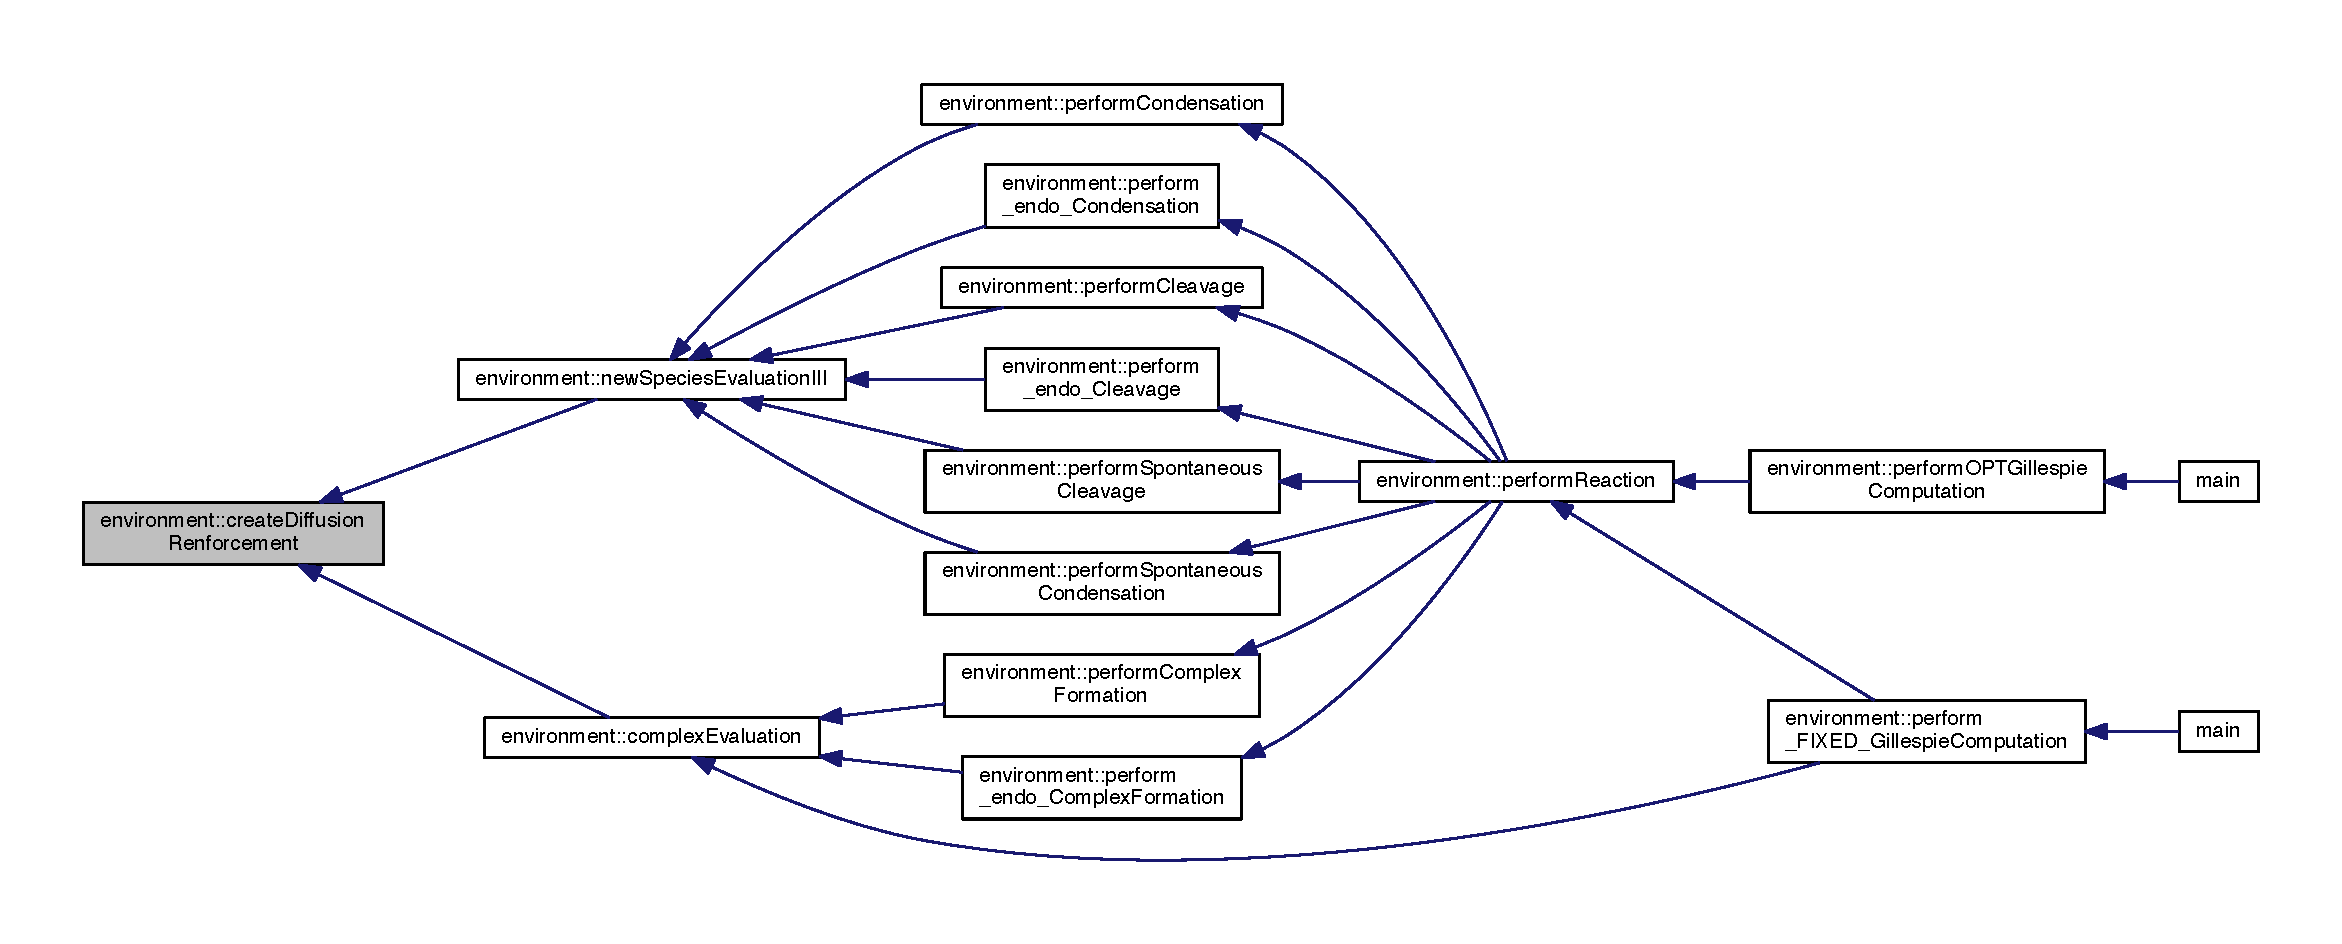
\includegraphics[width=350pt]{a00013_af795a4d1f04dfbfcbdf321e20e74f9c2_icgraph}
\end{center}
\end{figure}


\hypertarget{a00013_af795a4d1f04dfbfcbdf321e20e74f9c2}{\index{environment@{environment}!create\+Diffusion\+Renforcement@{create\+Diffusion\+Renforcement}}
\index{create\+Diffusion\+Renforcement@{create\+Diffusion\+Renforcement}!environment@{environment}}
\subsubsection[{create\+Diffusion\+Renforcement}]{\setlength{\rightskip}{0pt plus 5cm}{\bf acs\+\_\+double} environment\+::create\+Diffusion\+Renforcement (
\begin{DoxyParamCaption}
\item[{{\bf acs\+\_\+double}}]{tmp\+Diff\+Enh, }
\item[{{\bf acs\+\_\+int}}]{tmp\+New\+Species\+Length}
\end{DoxyParamCaption}
)}}\label{a00013_af795a4d1f04dfbfcbdf321e20e74f9c2}
\hypertarget{a00013_a902df40829dad9a885122082ec8fff7a}{\index{environment@{environment}!create\+Influx\+Layers\+From\+File\+S\+T\+D@{create\+Influx\+Layers\+From\+File\+S\+T\+D}}
\index{create\+Influx\+Layers\+From\+File\+S\+T\+D@{create\+Influx\+Layers\+From\+File\+S\+T\+D}!environment@{environment}}
\subsubsection[{create\+Influx\+Layers\+From\+File\+S\+T\+D}]{\setlength{\rightskip}{0pt plus 5cm}bool environment\+::create\+Influx\+Layers\+From\+File\+S\+T\+D (
\begin{DoxyParamCaption}
\item[{string}]{tmp\+Influx\+File\+Path}
\end{DoxyParamCaption}
)}}\label{a00013_a902df40829dad9a885122082ec8fff7a}
Create influx layer from file C++ libraries \begin{DoxyVersion}{Version}
1.\+0 
\end{DoxyVersion}

\begin{DoxyParams}{Parameters}
{\em string} & tmp\+Influx\+File\+Path file path \\
\hline
\end{DoxyParams}
\begin{DoxyDate}{Date}
20130702 
\end{DoxyDate}


Definition at line 1572 of file environment.\+cpp.



Here is the caller graph for this function\+:\nopagebreak
\begin{figure}[H]
\begin{center}
\leavevmode
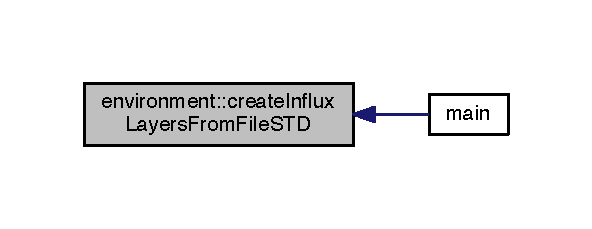
\includegraphics[width=284pt]{a00013_a902df40829dad9a885122082ec8fff7a_icgraph}
\end{center}
\end{figure}


\hypertarget{a00013_a902df40829dad9a885122082ec8fff7a}{\index{environment@{environment}!create\+Influx\+Layers\+From\+File\+S\+T\+D@{create\+Influx\+Layers\+From\+File\+S\+T\+D}}
\index{create\+Influx\+Layers\+From\+File\+S\+T\+D@{create\+Influx\+Layers\+From\+File\+S\+T\+D}!environment@{environment}}
\subsubsection[{create\+Influx\+Layers\+From\+File\+S\+T\+D}]{\setlength{\rightskip}{0pt plus 5cm}bool environment\+::create\+Influx\+Layers\+From\+File\+S\+T\+D (
\begin{DoxyParamCaption}
\item[{string}]{tmp\+Influx\+File\+Path}
\end{DoxyParamCaption}
)}}\label{a00013_a902df40829dad9a885122082ec8fff7a}
\hypertarget{a00013_a29eeb7a1b4689c10fd872e82179b4d84}{\index{environment@{environment}!create\+Initial\+Catalysis\+Layer\+From\+File\+S\+T\+D@{create\+Initial\+Catalysis\+Layer\+From\+File\+S\+T\+D}}
\index{create\+Initial\+Catalysis\+Layer\+From\+File\+S\+T\+D@{create\+Initial\+Catalysis\+Layer\+From\+File\+S\+T\+D}!environment@{environment}}
\subsubsection[{create\+Initial\+Catalysis\+Layer\+From\+File\+S\+T\+D}]{\setlength{\rightskip}{0pt plus 5cm}bool environment\+::create\+Initial\+Catalysis\+Layer\+From\+File\+S\+T\+D (
\begin{DoxyParamCaption}
\item[{string}]{tmp\+Catalysis\+File\+Path}
\end{DoxyParamCaption}
)}}\label{a00013_a29eeb7a1b4689c10fd872e82179b4d84}
Catalysis from file using standard C++ libraries \begin{DoxyVersion}{Version}
1.\+0 
\end{DoxyVersion}

\begin{DoxyParams}{Parameters}
{\em string} & tmp\+Species\+File\+Path file path \\
\hline
\end{DoxyParams}
\begin{DoxyDate}{Date}
20130702 
\end{DoxyDate}


Definition at line 1724 of file environment.\+cpp.



Here is the call graph for this function\+:\nopagebreak
\begin{figure}[H]
\begin{center}
\leavevmode
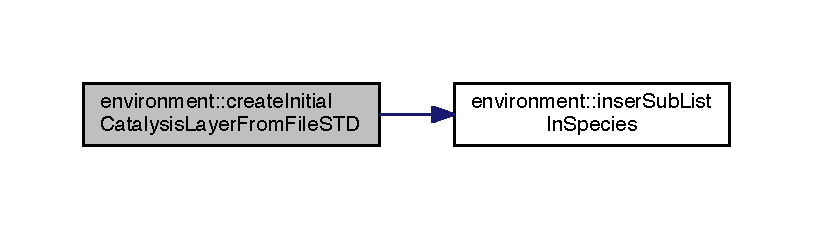
\includegraphics[width=350pt]{a00013_a29eeb7a1b4689c10fd872e82179b4d84_cgraph}
\end{center}
\end{figure}




Here is the caller graph for this function\+:\nopagebreak
\begin{figure}[H]
\begin{center}
\leavevmode
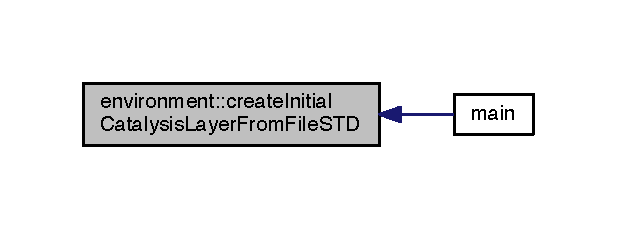
\includegraphics[width=296pt]{a00013_a29eeb7a1b4689c10fd872e82179b4d84_icgraph}
\end{center}
\end{figure}


\hypertarget{a00013_a29eeb7a1b4689c10fd872e82179b4d84}{\index{environment@{environment}!create\+Initial\+Catalysis\+Layer\+From\+File\+S\+T\+D@{create\+Initial\+Catalysis\+Layer\+From\+File\+S\+T\+D}}
\index{create\+Initial\+Catalysis\+Layer\+From\+File\+S\+T\+D@{create\+Initial\+Catalysis\+Layer\+From\+File\+S\+T\+D}!environment@{environment}}
\subsubsection[{create\+Initial\+Catalysis\+Layer\+From\+File\+S\+T\+D}]{\setlength{\rightskip}{0pt plus 5cm}bool environment\+::create\+Initial\+Catalysis\+Layer\+From\+File\+S\+T\+D (
\begin{DoxyParamCaption}
\item[{string}]{tmp\+Catalysis\+File\+Path}
\end{DoxyParamCaption}
)}}\label{a00013_a29eeb7a1b4689c10fd872e82179b4d84}
\hypertarget{a00013_a6dd31bae82367ebe7d6a6bb062b8cd07}{\index{environment@{environment}!create\+Initial\+Catalysis\+Layer\+From\+Specific\+File\+S\+T\+D@{create\+Initial\+Catalysis\+Layer\+From\+Specific\+File\+S\+T\+D}}
\index{create\+Initial\+Catalysis\+Layer\+From\+Specific\+File\+S\+T\+D@{create\+Initial\+Catalysis\+Layer\+From\+Specific\+File\+S\+T\+D}!environment@{environment}}
\subsubsection[{create\+Initial\+Catalysis\+Layer\+From\+Specific\+File\+S\+T\+D}]{\setlength{\rightskip}{0pt plus 5cm}bool environment\+::create\+Initial\+Catalysis\+Layer\+From\+Specific\+File\+S\+T\+D (
\begin{DoxyParamCaption}
\item[{string}]{tmp\+Catalysis\+File\+Path, }
\item[{{\bf acs\+\_\+int}}]{tmp\+Act\+G\+E\+N, }
\item[{{\bf acs\+\_\+int}}]{tmp\+Act\+S\+I\+M}
\end{DoxyParamCaption}
)}}\label{a00013_a6dd31bae82367ebe7d6a6bb062b8cd07}
catalysis from file using standard C++ libraries \begin{DoxyVersion}{Version}
1.\+0 
\end{DoxyVersion}

\begin{DoxyParams}{Parameters}
{\em string} & tmp\+Species\+File\+Path file path \\
\hline
\end{DoxyParams}
\begin{DoxyDate}{Date}
20130702 
\end{DoxyDate}


Definition at line 1766 of file environment.\+cpp.



Here is the call graph for this function\+:\nopagebreak
\begin{figure}[H]
\begin{center}
\leavevmode
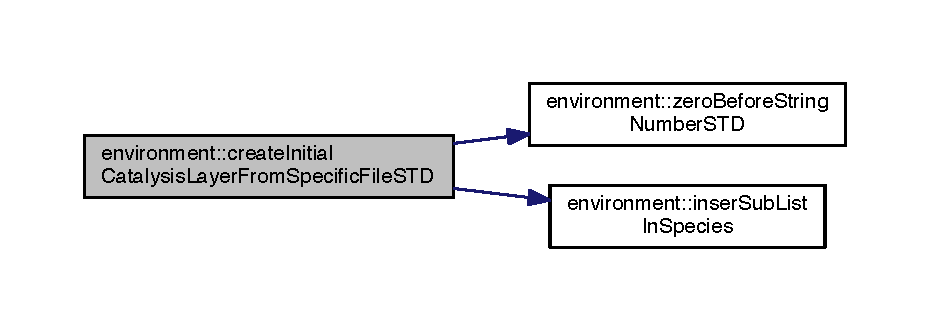
\includegraphics[width=350pt]{a00013_a6dd31bae82367ebe7d6a6bb062b8cd07_cgraph}
\end{center}
\end{figure}


\hypertarget{a00013_a6dd31bae82367ebe7d6a6bb062b8cd07}{\index{environment@{environment}!create\+Initial\+Catalysis\+Layer\+From\+Specific\+File\+S\+T\+D@{create\+Initial\+Catalysis\+Layer\+From\+Specific\+File\+S\+T\+D}}
\index{create\+Initial\+Catalysis\+Layer\+From\+Specific\+File\+S\+T\+D@{create\+Initial\+Catalysis\+Layer\+From\+Specific\+File\+S\+T\+D}!environment@{environment}}
\subsubsection[{create\+Initial\+Catalysis\+Layer\+From\+Specific\+File\+S\+T\+D}]{\setlength{\rightskip}{0pt plus 5cm}bool environment\+::create\+Initial\+Catalysis\+Layer\+From\+Specific\+File\+S\+T\+D (
\begin{DoxyParamCaption}
\item[{string}]{tmp\+Catalysis\+File\+Path, }
\item[{{\bf acs\+\_\+int}}]{tmp\+Act\+G\+E\+N, }
\item[{{\bf acs\+\_\+int}}]{tmp\+Act\+S\+I\+M}
\end{DoxyParamCaption}
)}}\label{a00013_a6dd31bae82367ebe7d6a6bb062b8cd07}
\hypertarget{a00013_aee77384e63261db28ef5677844bdbaf6}{\index{environment@{environment}!create\+Initial\+Molecules\+Population\+From\+File\+S\+T\+D@{create\+Initial\+Molecules\+Population\+From\+File\+S\+T\+D}}
\index{create\+Initial\+Molecules\+Population\+From\+File\+S\+T\+D@{create\+Initial\+Molecules\+Population\+From\+File\+S\+T\+D}!environment@{environment}}
\subsubsection[{create\+Initial\+Molecules\+Population\+From\+File\+S\+T\+D}]{\setlength{\rightskip}{0pt plus 5cm}bool environment\+::create\+Initial\+Molecules\+Population\+From\+File\+S\+T\+D (
\begin{DoxyParamCaption}
\item[{string}]{tmp\+Species\+File\+Path}
\end{DoxyParamCaption}
)}}\label{a00013_aee77384e63261db28ef5677844bdbaf6}
Initial molecule population creation from file using standard C++ libraries \begin{DoxyVersion}{Version}
1.\+0 
\end{DoxyVersion}

\begin{DoxyParams}{Parameters}
{\em string} & tmp\+Species\+File\+Path file path \\
\hline
\end{DoxyParams}
\begin{DoxyDate}{Date}
20130702 
\end{DoxyDate}


Definition at line 1249 of file environment.\+cpp.



Here is the call graph for this function\+:\nopagebreak
\begin{figure}[H]
\begin{center}
\leavevmode
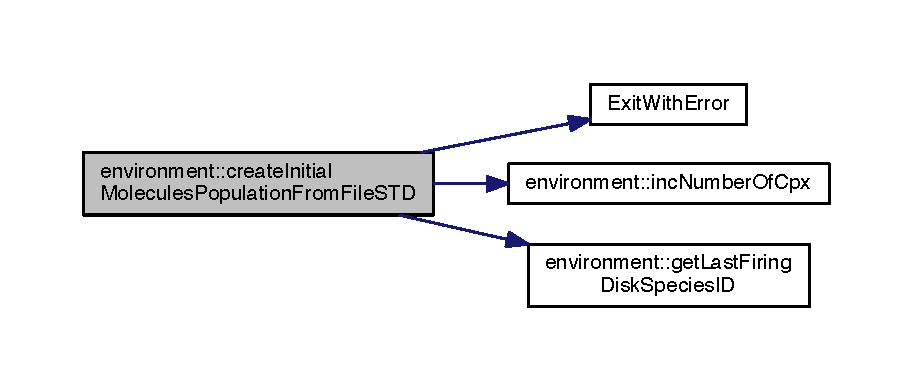
\includegraphics[width=350pt]{a00013_aee77384e63261db28ef5677844bdbaf6_cgraph}
\end{center}
\end{figure}




Here is the caller graph for this function\+:\nopagebreak
\begin{figure}[H]
\begin{center}
\leavevmode
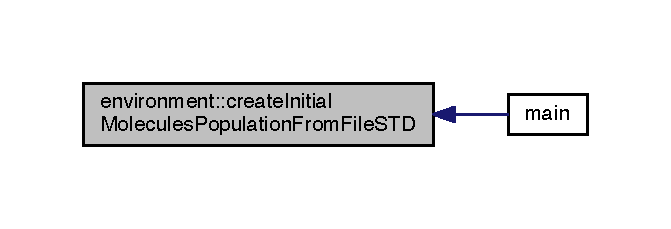
\includegraphics[width=322pt]{a00013_aee77384e63261db28ef5677844bdbaf6_icgraph}
\end{center}
\end{figure}


\hypertarget{a00013_af6db92c710f2588ba7dff1165e26d538}{\index{environment@{environment}!create\+Initial\+Molecules\+Population\+From\+File\+S\+T\+D@{create\+Initial\+Molecules\+Population\+From\+File\+S\+T\+D}}
\index{create\+Initial\+Molecules\+Population\+From\+File\+S\+T\+D@{create\+Initial\+Molecules\+Population\+From\+File\+S\+T\+D}!environment@{environment}}
\subsubsection[{create\+Initial\+Molecules\+Population\+From\+File\+S\+T\+D}]{\setlength{\rightskip}{0pt plus 5cm}bool environment\+::create\+Initial\+Molecules\+Population\+From\+File\+S\+T\+D (
\begin{DoxyParamCaption}
\item[{string}]{tmp\+Species\+File\+Path, }
\item[{{\bf M\+T\+Rand} \&}]{tmp\+Rnd\+Double\+Gen}
\end{DoxyParamCaption}
)}}\label{a00013_af6db92c710f2588ba7dff1165e26d538}
Initial molecule population creation from file using standard C++ libraries \begin{DoxyVersion}{Version}
1.\+0 
\end{DoxyVersion}

\begin{DoxyParams}{Parameters}
{\em string} & tmp\+Species\+File\+Path file path \\
\hline
\end{DoxyParams}
\begin{DoxyDate}{Date}
20130702 
\end{DoxyDate}


Definition at line 1261 of file environment.\+cpp.



Here is the call graph for this function\+:\nopagebreak
\begin{figure}[H]
\begin{center}
\leavevmode
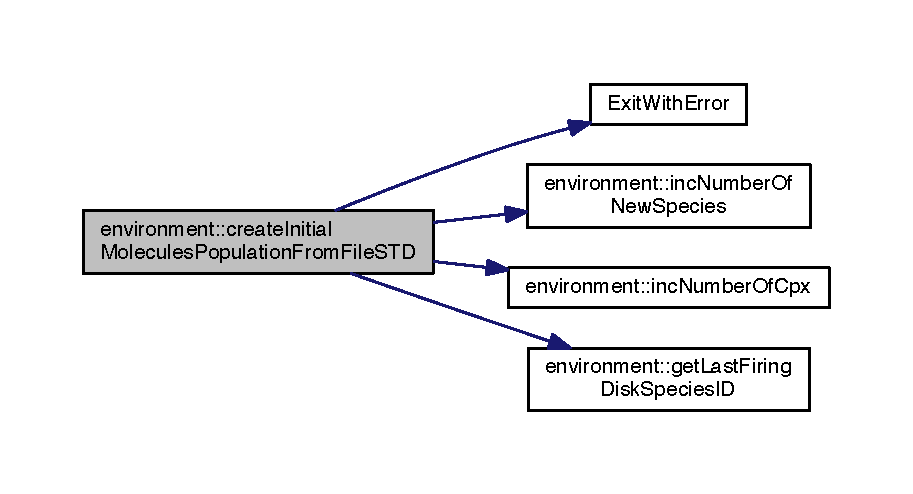
\includegraphics[width=350pt]{a00013_af6db92c710f2588ba7dff1165e26d538_cgraph}
\end{center}
\end{figure}


\hypertarget{a00013_aa70e1394bf2240f6e5f14d4cbf369a3b}{\index{environment@{environment}!create\+Initial\+Molecules\+Population\+From\+Specific\+File\+S\+T\+D@{create\+Initial\+Molecules\+Population\+From\+Specific\+File\+S\+T\+D}}
\index{create\+Initial\+Molecules\+Population\+From\+Specific\+File\+S\+T\+D@{create\+Initial\+Molecules\+Population\+From\+Specific\+File\+S\+T\+D}!environment@{environment}}
\subsubsection[{create\+Initial\+Molecules\+Population\+From\+Specific\+File\+S\+T\+D}]{\setlength{\rightskip}{0pt plus 5cm}bool environment\+::create\+Initial\+Molecules\+Population\+From\+Specific\+File\+S\+T\+D (
\begin{DoxyParamCaption}
\item[{string}]{tmp\+Species\+File\+Path, }
\item[{{\bf acs\+\_\+int}}]{tmp\+Act\+G\+E\+N, }
\item[{{\bf acs\+\_\+int}}]{tmp\+Act\+S\+I\+M}
\end{DoxyParamCaption}
)}}\label{a00013_aa70e1394bf2240f6e5f14d4cbf369a3b}
Initial molecule population creation from file \begin{DoxyVersion}{Version}
1.\+0 
\end{DoxyVersion}

\begin{DoxyParams}{Parameters}
{\em Q\+String} & tmp\+Species\+File\+Path file path Initial molecule population creation. Species are uploaed from a S\+P\+E\+C\+I\+F\+I\+C file created using actual generation and simuation \\
\hline
\end{DoxyParams}
\begin{DoxyVersion}{Version}
1.\+0 
\end{DoxyVersion}

\begin{DoxyParams}{Parameters}
{\em Q\+String} & tmp\+Species\+File\+Path file path Initial molecule population creation. Species are uploaed from a S\+P\+E\+C\+I\+F\+I\+C file created using actual generation and simuation (standard C++ libraries) \\
\hline
\end{DoxyParams}
\begin{DoxyVersion}{Version}
1.\+0 
\end{DoxyVersion}

\begin{DoxyParams}{Parameters}
{\em Q\+String} & tmp\+Species\+File\+Path file path \\
\hline
\end{DoxyParams}


Definition at line 1478 of file environment.\+cpp.



Here is the call graph for this function\+:\nopagebreak
\begin{figure}[H]
\begin{center}
\leavevmode
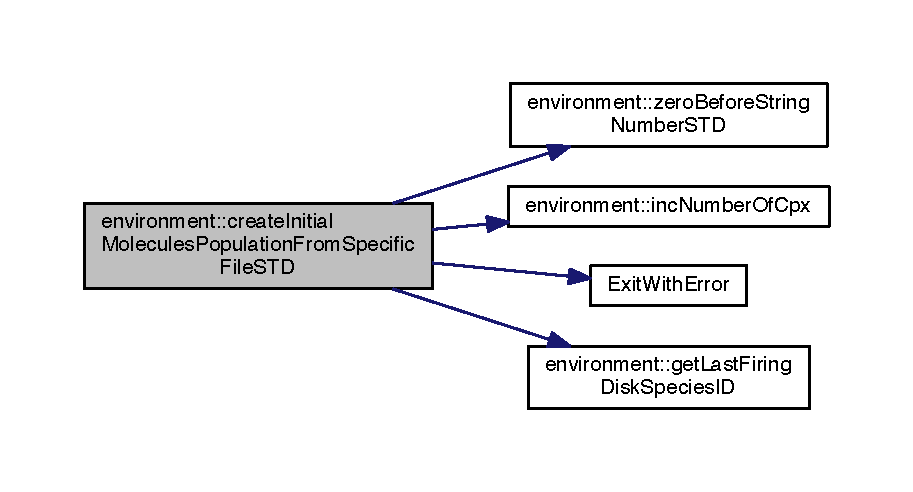
\includegraphics[width=350pt]{a00013_aa70e1394bf2240f6e5f14d4cbf369a3b_cgraph}
\end{center}
\end{figure}


\hypertarget{a00013_ab85fdf18a88fb51afc48eba31d0ed1b2}{\index{environment@{environment}!create\+Initial\+Molecules\+Population\+From\+Specific\+File\+S\+T\+D@{create\+Initial\+Molecules\+Population\+From\+Specific\+File\+S\+T\+D}}
\index{create\+Initial\+Molecules\+Population\+From\+Specific\+File\+S\+T\+D@{create\+Initial\+Molecules\+Population\+From\+Specific\+File\+S\+T\+D}!environment@{environment}}
\subsubsection[{create\+Initial\+Molecules\+Population\+From\+Specific\+File\+S\+T\+D}]{\setlength{\rightskip}{0pt plus 5cm}bool environment\+::create\+Initial\+Molecules\+Population\+From\+Specific\+File\+S\+T\+D (
\begin{DoxyParamCaption}
\item[{string}]{tmp\+Species\+File\+Path, }
\item[{{\bf acs\+\_\+int}}]{tmp\+Act\+G\+E\+N, }
\item[{{\bf acs\+\_\+int}}]{tmp\+Act\+S\+I\+M, }
\item[{{\bf M\+T\+Rand} \&}]{tmp\+Rnd\+Double\+Gen}
\end{DoxyParamCaption}
)}}\label{a00013_ab85fdf18a88fb51afc48eba31d0ed1b2}
Initial molecule population creation from file \begin{DoxyVersion}{Version}
1.\+0 
\end{DoxyVersion}

\begin{DoxyParams}{Parameters}
{\em Q\+String} & tmp\+Species\+File\+Path file path Initial molecule population creation. Species are uploaed from a S\+P\+E\+C\+I\+F\+I\+C file created using actual generation and simuation \\
\hline
\end{DoxyParams}
\begin{DoxyVersion}{Version}
1.\+0 
\end{DoxyVersion}

\begin{DoxyParams}{Parameters}
{\em Q\+String} & tmp\+Species\+File\+Path file path Initial molecule population creation. Species are uploaed from a S\+P\+E\+C\+I\+F\+I\+C file created using actual generation and simuation (standard C++ libraries) \\
\hline
\end{DoxyParams}
\begin{DoxyVersion}{Version}
1.\+0 
\end{DoxyVersion}

\begin{DoxyParams}{Parameters}
{\em Q\+String} & tmp\+Species\+File\+Path file path \\
\hline
\end{DoxyParams}


Definition at line 1490 of file environment.\+cpp.



Here is the call graph for this function\+:\nopagebreak
\begin{figure}[H]
\begin{center}
\leavevmode
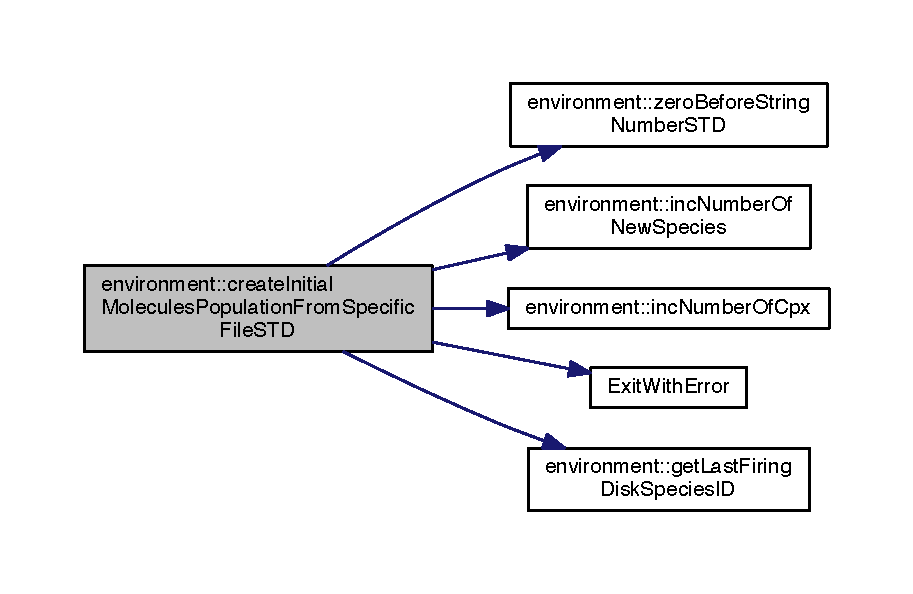
\includegraphics[width=350pt]{a00013_ab85fdf18a88fb51afc48eba31d0ed1b2_cgraph}
\end{center}
\end{figure}


\hypertarget{a00013_a2f181e0d3ad1e8062ba0a8c9358ebc58}{\index{environment@{environment}!create\+Initial\+Reactions\+Layer\+From\+File\+S\+T\+D@{create\+Initial\+Reactions\+Layer\+From\+File\+S\+T\+D}}
\index{create\+Initial\+Reactions\+Layer\+From\+File\+S\+T\+D@{create\+Initial\+Reactions\+Layer\+From\+File\+S\+T\+D}!environment@{environment}}
\subsubsection[{create\+Initial\+Reactions\+Layer\+From\+File\+S\+T\+D}]{\setlength{\rightskip}{0pt plus 5cm}bool environment\+::create\+Initial\+Reactions\+Layer\+From\+File\+S\+T\+D (
\begin{DoxyParamCaption}
\item[{string}]{tmp\+Species\+File\+Path}
\end{DoxyParamCaption}
)}}\label{a00013_a2f181e0d3ad1e8062ba0a8c9358ebc58}
Reactions from file using standard C++ libraries \begin{DoxyVersion}{Version}
1.\+0 
\end{DoxyVersion}

\begin{DoxyParams}{Parameters}
{\em string} & tmp\+Species\+File\+Path file path \\
\hline
\end{DoxyParams}
\begin{DoxyDate}{Date}
20130702 
\end{DoxyDate}


Definition at line 1635 of file environment.\+cpp.



Here is the caller graph for this function\+:\nopagebreak
\begin{figure}[H]
\begin{center}
\leavevmode
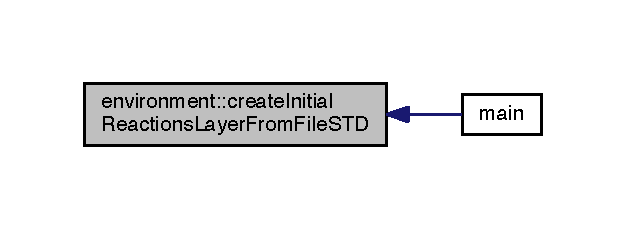
\includegraphics[width=300pt]{a00013_a2f181e0d3ad1e8062ba0a8c9358ebc58_icgraph}
\end{center}
\end{figure}


\hypertarget{a00013_a2f181e0d3ad1e8062ba0a8c9358ebc58}{\index{environment@{environment}!create\+Initial\+Reactions\+Layer\+From\+File\+S\+T\+D@{create\+Initial\+Reactions\+Layer\+From\+File\+S\+T\+D}}
\index{create\+Initial\+Reactions\+Layer\+From\+File\+S\+T\+D@{create\+Initial\+Reactions\+Layer\+From\+File\+S\+T\+D}!environment@{environment}}
\subsubsection[{create\+Initial\+Reactions\+Layer\+From\+File\+S\+T\+D}]{\setlength{\rightskip}{0pt plus 5cm}bool environment\+::create\+Initial\+Reactions\+Layer\+From\+File\+S\+T\+D (
\begin{DoxyParamCaption}
\item[{string}]{tmp\+Species\+File\+Path}
\end{DoxyParamCaption}
)}}\label{a00013_a2f181e0d3ad1e8062ba0a8c9358ebc58}
\hypertarget{a00013_a743956229b11d7860dbc89a18f869586}{\index{environment@{environment}!create\+Initial\+Reactions\+Layer\+From\+Specific\+File\+S\+T\+D@{create\+Initial\+Reactions\+Layer\+From\+Specific\+File\+S\+T\+D}}
\index{create\+Initial\+Reactions\+Layer\+From\+Specific\+File\+S\+T\+D@{create\+Initial\+Reactions\+Layer\+From\+Specific\+File\+S\+T\+D}!environment@{environment}}
\subsubsection[{create\+Initial\+Reactions\+Layer\+From\+Specific\+File\+S\+T\+D}]{\setlength{\rightskip}{0pt plus 5cm}bool environment\+::create\+Initial\+Reactions\+Layer\+From\+Specific\+File\+S\+T\+D (
\begin{DoxyParamCaption}
\item[{string}]{tmp\+Reactions\+File\+Path, }
\item[{{\bf acs\+\_\+int}}]{tmp\+Act\+G\+E\+N, }
\item[{{\bf acs\+\_\+int}}]{tmp\+Act\+S\+I\+M}
\end{DoxyParamCaption}
)}}\label{a00013_a743956229b11d7860dbc89a18f869586}
Reactions from file using standard C++ libraries \begin{DoxyVersion}{Version}
1.\+0 
\end{DoxyVersion}

\begin{DoxyParams}{Parameters}
{\em string} & tmp\+Species\+File\+Path file path \\
\hline
\end{DoxyParams}
\begin{DoxyDate}{Date}
20130702 
\end{DoxyDate}


Definition at line 1674 of file environment.\+cpp.



Here is the call graph for this function\+:\nopagebreak
\begin{figure}[H]
\begin{center}
\leavevmode
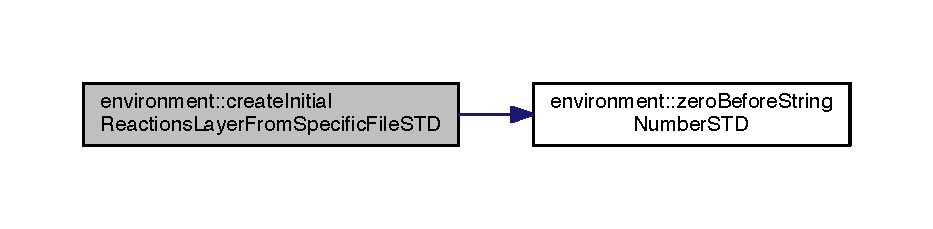
\includegraphics[width=350pt]{a00013_a743956229b11d7860dbc89a18f869586_cgraph}
\end{center}
\end{figure}


\hypertarget{a00013_a743956229b11d7860dbc89a18f869586}{\index{environment@{environment}!create\+Initial\+Reactions\+Layer\+From\+Specific\+File\+S\+T\+D@{create\+Initial\+Reactions\+Layer\+From\+Specific\+File\+S\+T\+D}}
\index{create\+Initial\+Reactions\+Layer\+From\+Specific\+File\+S\+T\+D@{create\+Initial\+Reactions\+Layer\+From\+Specific\+File\+S\+T\+D}!environment@{environment}}
\subsubsection[{create\+Initial\+Reactions\+Layer\+From\+Specific\+File\+S\+T\+D}]{\setlength{\rightskip}{0pt plus 5cm}bool environment\+::create\+Initial\+Reactions\+Layer\+From\+Specific\+File\+S\+T\+D (
\begin{DoxyParamCaption}
\item[{string}]{tmp\+Reactions\+File\+Path, }
\item[{{\bf acs\+\_\+int}}]{tmp\+Act\+G\+E\+N, }
\item[{{\bf acs\+\_\+int}}]{tmp\+Act\+S\+I\+M}
\end{DoxyParamCaption}
)}}\label{a00013_a743956229b11d7860dbc89a18f869586}
\hypertarget{a00013_abe1a616460ea328067874df715679319}{\index{environment@{environment}!create\+Nrg\+Boolean\+Functions\+From\+File\+S\+T\+D@{create\+Nrg\+Boolean\+Functions\+From\+File\+S\+T\+D}}
\index{create\+Nrg\+Boolean\+Functions\+From\+File\+S\+T\+D@{create\+Nrg\+Boolean\+Functions\+From\+File\+S\+T\+D}!environment@{environment}}
\subsubsection[{create\+Nrg\+Boolean\+Functions\+From\+File\+S\+T\+D}]{\setlength{\rightskip}{0pt plus 5cm}bool environment\+::create\+Nrg\+Boolean\+Functions\+From\+File\+S\+T\+D (
\begin{DoxyParamCaption}
\item[{string}]{tmp\+Bool\+Nrg\+File\+Path}
\end{DoxyParamCaption}
)}}\label{a00013_abe1a616460ea328067874df715679319}
load energy boolean function (in decimal format) -\/ Standard C++ \begin{DoxyVersion}{Version}
1.\+0 
\end{DoxyVersion}

\begin{DoxyParams}{Parameters}
{\em string} & tmp\+Bool\+Nrg\+File\+Path file path \\
\hline
\end{DoxyParams}
\begin{DoxyDate}{Date}
20130702 
\end{DoxyDate}


Definition at line 1604 of file environment.\+cpp.



Here is the caller graph for this function\+:\nopagebreak
\begin{figure}[H]
\begin{center}
\leavevmode
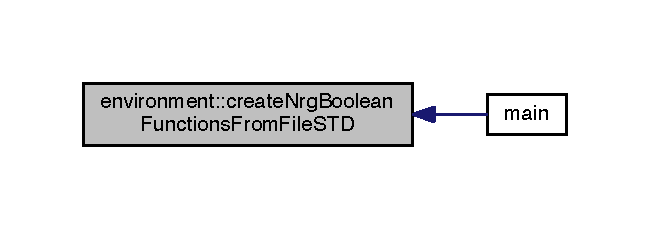
\includegraphics[width=312pt]{a00013_abe1a616460ea328067874df715679319_icgraph}
\end{center}
\end{figure}


\hypertarget{a00013_abe1a616460ea328067874df715679319}{\index{environment@{environment}!create\+Nrg\+Boolean\+Functions\+From\+File\+S\+T\+D@{create\+Nrg\+Boolean\+Functions\+From\+File\+S\+T\+D}}
\index{create\+Nrg\+Boolean\+Functions\+From\+File\+S\+T\+D@{create\+Nrg\+Boolean\+Functions\+From\+File\+S\+T\+D}!environment@{environment}}
\subsubsection[{create\+Nrg\+Boolean\+Functions\+From\+File\+S\+T\+D}]{\setlength{\rightskip}{0pt plus 5cm}bool environment\+::create\+Nrg\+Boolean\+Functions\+From\+File\+S\+T\+D (
\begin{DoxyParamCaption}
\item[{string}]{tmp\+Bool\+Nrg\+File\+Path}
\end{DoxyParamCaption}
)}}\label{a00013_abe1a616460ea328067874df715679319}
\hypertarget{a00013_a76794f37d6d94b7504c58f0f4a4709ca}{\index{environment@{environment}!create\+Reactions\+For\+This\+Species@{create\+Reactions\+For\+This\+Species}}
\index{create\+Reactions\+For\+This\+Species@{create\+Reactions\+For\+This\+Species}!environment@{environment}}
\subsubsection[{create\+Reactions\+For\+This\+Species}]{\setlength{\rightskip}{0pt plus 5cm}bool environment\+::create\+Reactions\+For\+This\+Species (
\begin{DoxyParamCaption}
\item[{{\bf acs\+\_\+long\+Int}}]{tmps\+I\+D, }
\item[{{\bf acs\+\_\+int}}]{tmp\+Reactions\+For\+This\+Species, }
\item[{{\bf M\+T\+Rand} \&}]{tmp\+\_\+\+Rnd\+Double\+Gen, }
\item[{vector$<$ {\bf acs\+\_\+long\+Int} $>$ \&}]{tmp\+I\+D\+Of\+Candidate\+Species, }
\item[{{\bf acs\+\_\+int}}]{tmp\+Rct\+Creation\+Type}
\end{DoxyParamCaption}
)}}\label{a00013_a76794f37d6d94b7504c58f0f4a4709ca}
Creation of all the reactions related to one specific species \begin{DoxyVersion}{Version}
1.\+1 
\end{DoxyVersion}
\begin{DoxyDate}{Date}
2011/07/07 
\end{DoxyDate}

\begin{DoxyParams}{Parameters}
{\em acs\+\_\+long\+Int} & tmps\+I\+D species vector I\+D \\
\hline
{\em acs\+\_\+int} & tmp\+Reactions\+For\+This\+Species number of reactions to create for this species \\
\hline
{\em M\+T\+Rand\&} & tmp\+\_\+\+Rnd\+Double\+Gen random number generator \\
\hline
{\em vector$<$acs\+\_\+long\+Int$>$\&} & tmp\+I\+D\+Of\+Candidate\+Species I\+D of the species avalaible for the reaction \\
\hline
{\em acs\+\_\+int} & tmp\+Rct\+Creation\+Type N\+E\+W\+R\+E\+A\+C\+T\+I\+O\+N or U\+P\+G\+R\+A\+D\+E\+R\+E\+A\+C\+T\+I\+O\+N\+S \\
\hline
\end{DoxyParams}


Definition at line 525 of file environment.\+cpp.



Here is the call graph for this function\+:\nopagebreak
\begin{figure}[H]
\begin{center}
\leavevmode
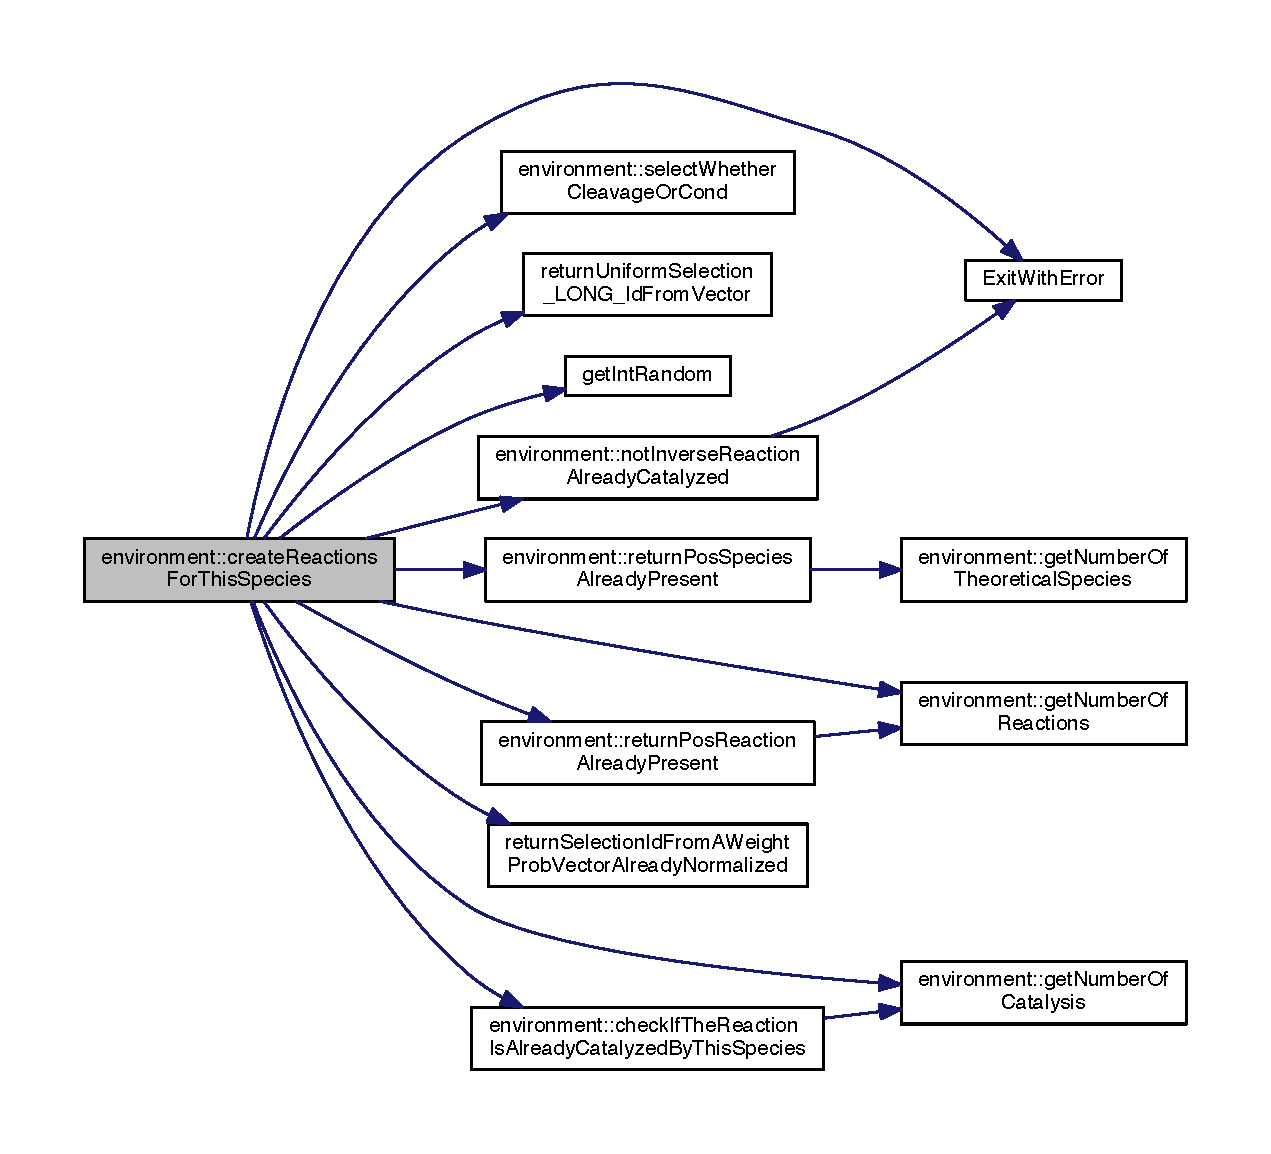
\includegraphics[width=350pt]{a00013_a76794f37d6d94b7504c58f0f4a4709ca_cgraph}
\end{center}
\end{figure}




Here is the caller graph for this function\+:\nopagebreak
\begin{figure}[H]
\begin{center}
\leavevmode
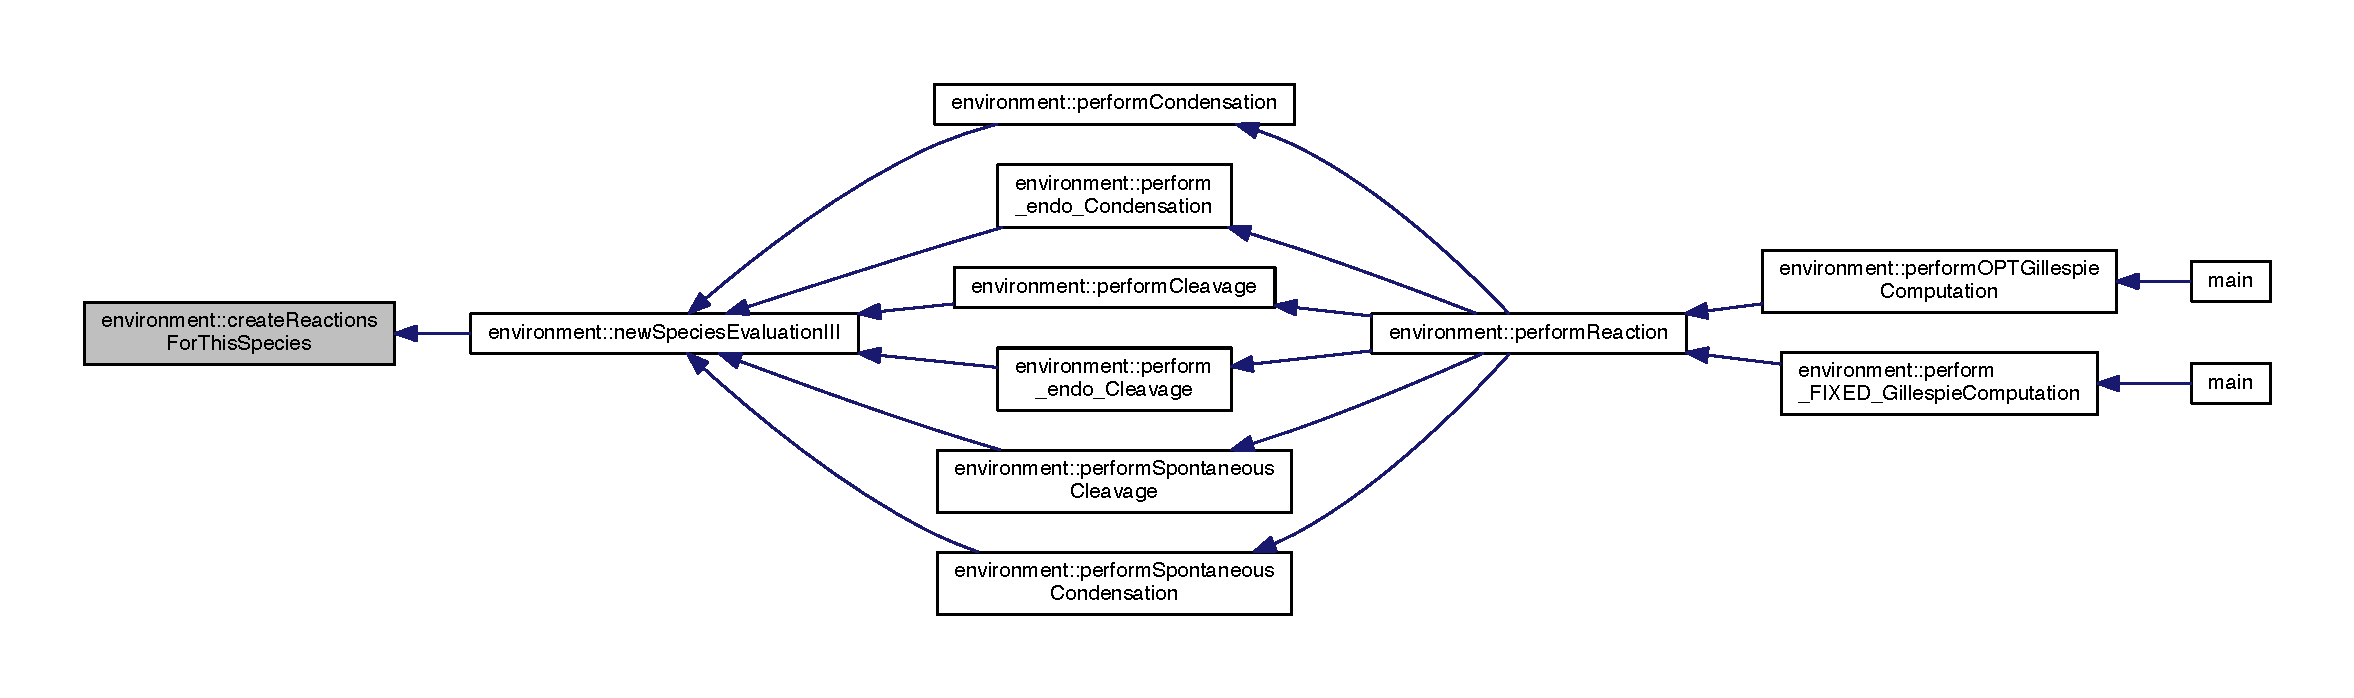
\includegraphics[width=350pt]{a00013_a76794f37d6d94b7504c58f0f4a4709ca_icgraph}
\end{center}
\end{figure}


\hypertarget{a00013_a76794f37d6d94b7504c58f0f4a4709ca}{\index{environment@{environment}!create\+Reactions\+For\+This\+Species@{create\+Reactions\+For\+This\+Species}}
\index{create\+Reactions\+For\+This\+Species@{create\+Reactions\+For\+This\+Species}!environment@{environment}}
\subsubsection[{create\+Reactions\+For\+This\+Species}]{\setlength{\rightskip}{0pt plus 5cm}bool environment\+::create\+Reactions\+For\+This\+Species (
\begin{DoxyParamCaption}
\item[{{\bf acs\+\_\+long\+Int}}]{tmps\+I\+D, }
\item[{{\bf acs\+\_\+int}}]{tmp\+Reactions\+For\+This\+Species, }
\item[{{\bf M\+T\+Rand} \&}]{tmp\+\_\+\+Rnd\+Double\+Gen, }
\item[{vector$<$ {\bf acs\+\_\+long\+Int} $>$ \&}]{tmp\+I\+D\+Of\+Candidate\+Species, }
\item[{{\bf acs\+\_\+int}}]{tmp\+Rct\+Creation\+Type}
\end{DoxyParamCaption}
)}}\label{a00013_a76794f37d6d94b7504c58f0f4a4709ca}
\hypertarget{a00013_a16d09f818d3012f88e8e4c9a7759b6bd}{\index{environment@{environment}!dec\+Cpx\+Procedure@{dec\+Cpx\+Procedure}}
\index{dec\+Cpx\+Procedure@{dec\+Cpx\+Procedure}!environment@{environment}}
\subsubsection[{dec\+Cpx\+Procedure}]{\setlength{\rightskip}{0pt plus 5cm}void environment\+::dec\+Cpx\+Procedure (
\begin{DoxyParamCaption}
\item[{{\bf acs\+\_\+int}}]{tmp\+\_\+\+I\+D}
\end{DoxyParamCaption}
)\hspace{0.3cm}{\ttfamily [inline]}}}\label{a00013_a16d09f818d3012f88e8e4c9a7759b6bd}


Definition at line 298 of file environment.\+h.



Here is the call graph for this function\+:\nopagebreak
\begin{figure}[H]
\begin{center}
\leavevmode
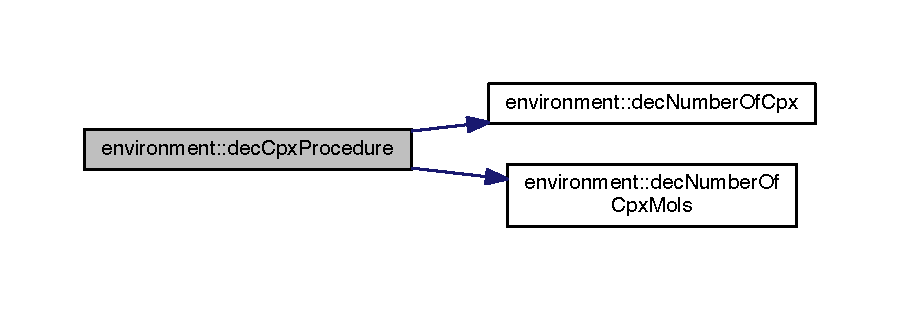
\includegraphics[width=350pt]{a00013_a16d09f818d3012f88e8e4c9a7759b6bd_cgraph}
\end{center}
\end{figure}




Here is the caller graph for this function\+:\nopagebreak
\begin{figure}[H]
\begin{center}
\leavevmode
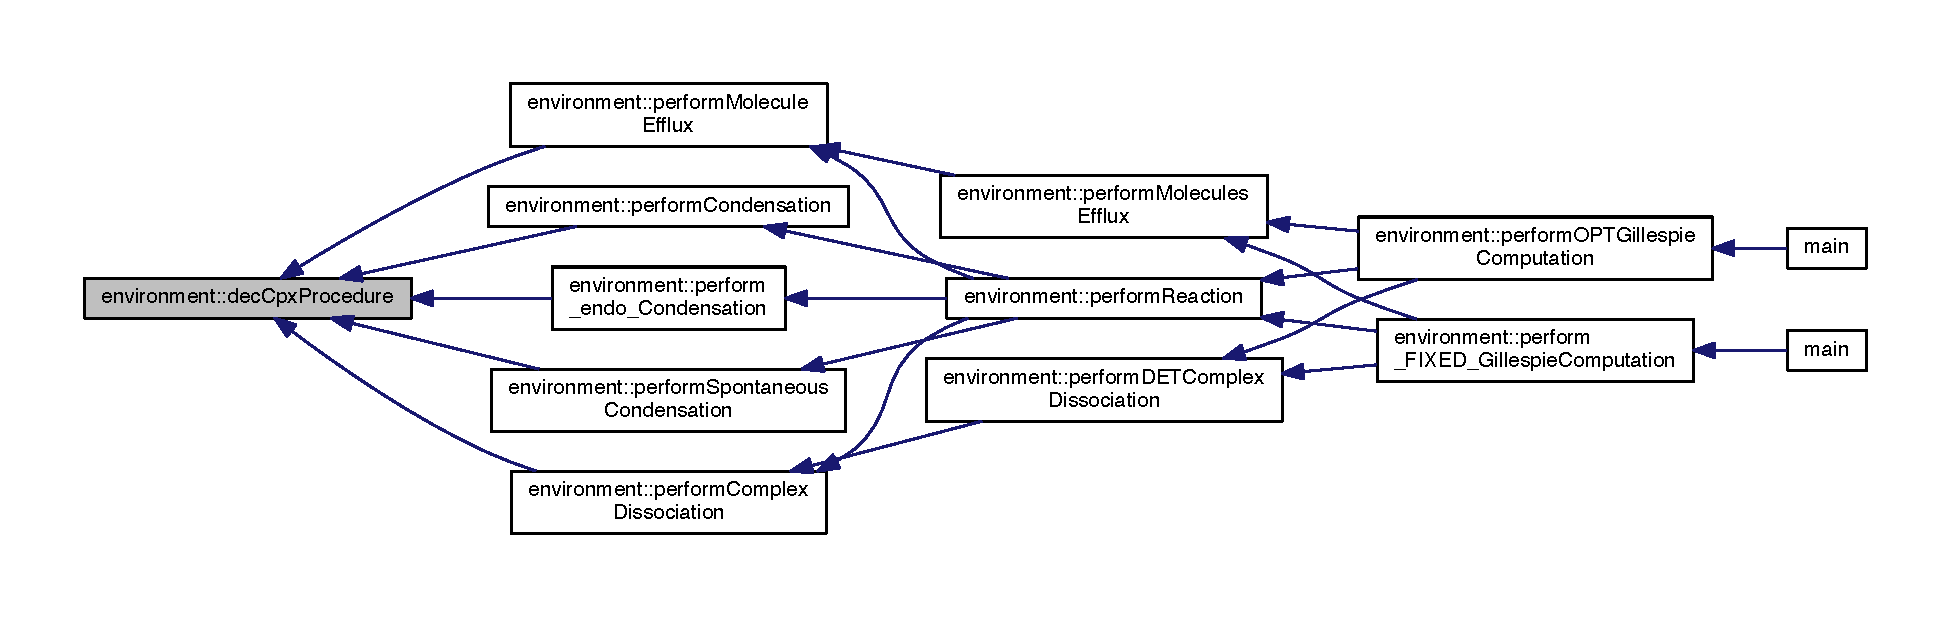
\includegraphics[width=350pt]{a00013_a16d09f818d3012f88e8e4c9a7759b6bd_icgraph}
\end{center}
\end{figure}


\hypertarget{a00013_a16d09f818d3012f88e8e4c9a7759b6bd}{\index{environment@{environment}!dec\+Cpx\+Procedure@{dec\+Cpx\+Procedure}}
\index{dec\+Cpx\+Procedure@{dec\+Cpx\+Procedure}!environment@{environment}}
\subsubsection[{dec\+Cpx\+Procedure}]{\setlength{\rightskip}{0pt plus 5cm}void environment\+::dec\+Cpx\+Procedure (
\begin{DoxyParamCaption}
\item[{{\bf acs\+\_\+int}}]{tmp\+\_\+\+I\+D}
\end{DoxyParamCaption}
)\hspace{0.3cm}{\ttfamily [inline]}}}\label{a00013_a16d09f818d3012f88e8e4c9a7759b6bd}


Definition at line 328 of file environment.\+h.



Here is the call graph for this function\+:\nopagebreak
\begin{figure}[H]
\begin{center}
\leavevmode
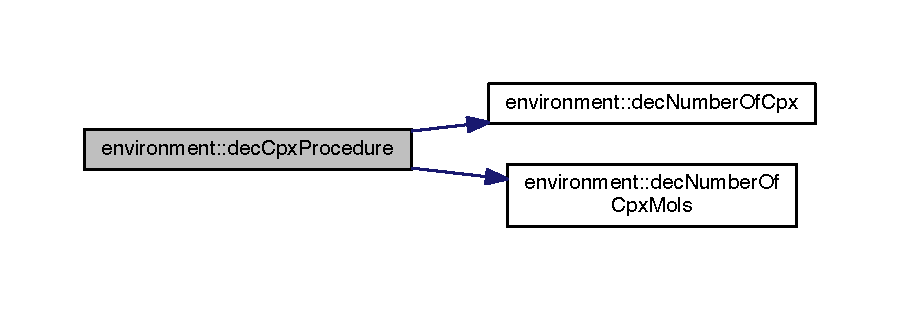
\includegraphics[width=350pt]{a00013_a16d09f818d3012f88e8e4c9a7759b6bd_cgraph}
\end{center}
\end{figure}


\hypertarget{a00013_a10fad450cf5ef3a1c7cf75d616105069}{\index{environment@{environment}!dec\+Mol\+Species\+Procedure@{dec\+Mol\+Species\+Procedure}}
\index{dec\+Mol\+Species\+Procedure@{dec\+Mol\+Species\+Procedure}!environment@{environment}}
\subsubsection[{dec\+Mol\+Species\+Procedure}]{\setlength{\rightskip}{0pt plus 5cm}void environment\+::dec\+Mol\+Species\+Procedure (
\begin{DoxyParamCaption}
\item[{{\bf acs\+\_\+int}}]{tmp\+\_\+\+I\+D}
\end{DoxyParamCaption}
)\hspace{0.3cm}{\ttfamily [inline]}}}\label{a00013_a10fad450cf5ef3a1c7cf75d616105069}


Definition at line 297 of file environment.\+h.



Here is the call graph for this function\+:\nopagebreak
\begin{figure}[H]
\begin{center}
\leavevmode
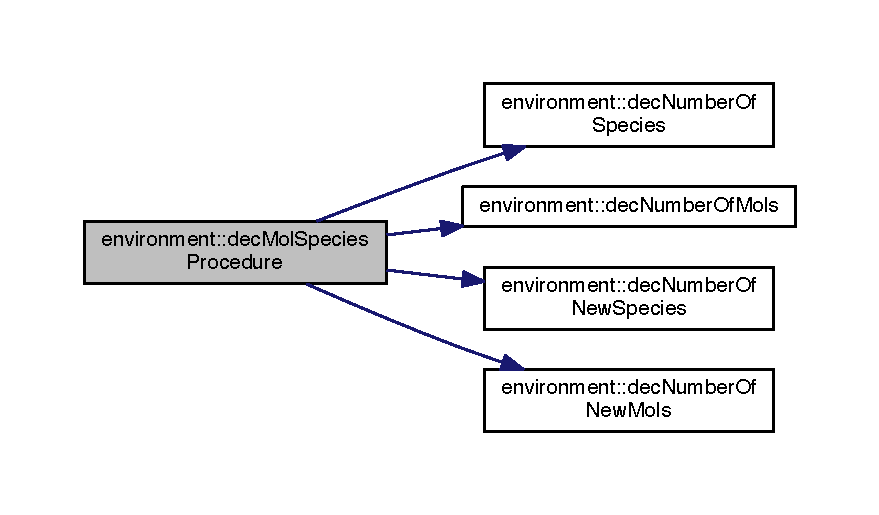
\includegraphics[width=350pt]{a00013_a10fad450cf5ef3a1c7cf75d616105069_cgraph}
\end{center}
\end{figure}




Here is the caller graph for this function\+:\nopagebreak
\begin{figure}[H]
\begin{center}
\leavevmode
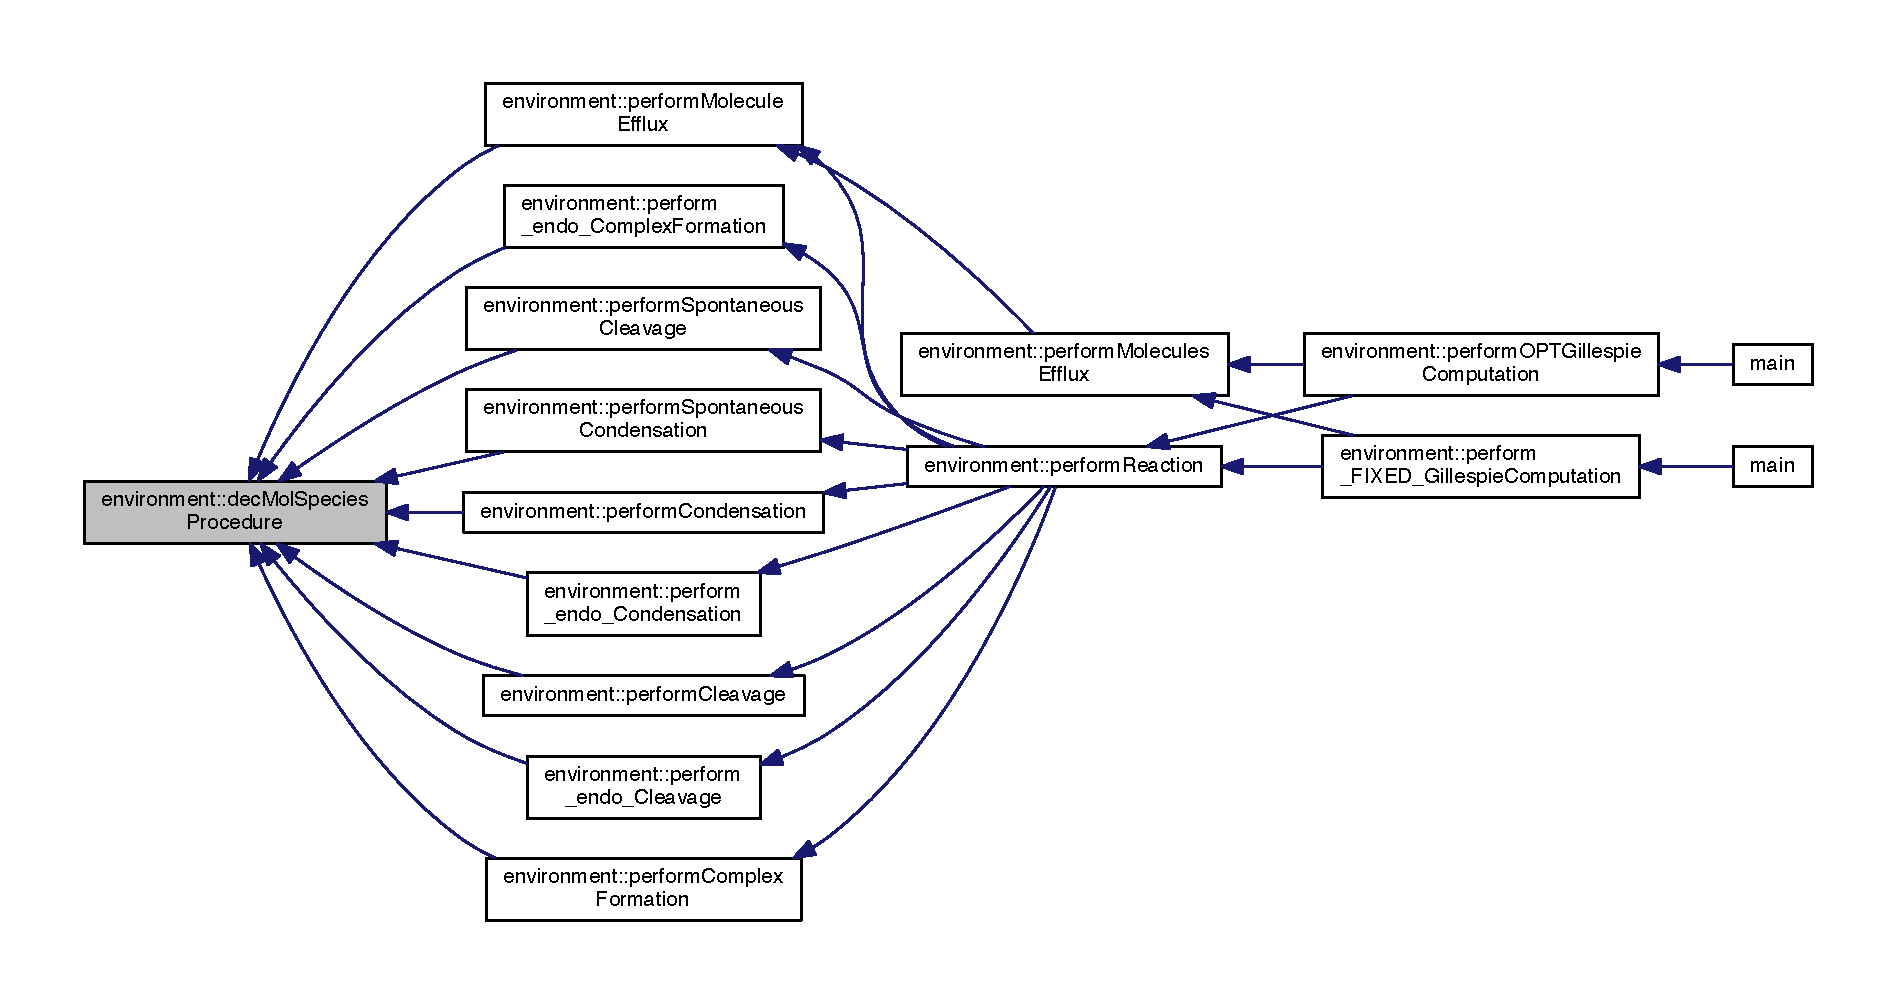
\includegraphics[width=350pt]{a00013_a10fad450cf5ef3a1c7cf75d616105069_icgraph}
\end{center}
\end{figure}


\hypertarget{a00013_a10fad450cf5ef3a1c7cf75d616105069}{\index{environment@{environment}!dec\+Mol\+Species\+Procedure@{dec\+Mol\+Species\+Procedure}}
\index{dec\+Mol\+Species\+Procedure@{dec\+Mol\+Species\+Procedure}!environment@{environment}}
\subsubsection[{dec\+Mol\+Species\+Procedure}]{\setlength{\rightskip}{0pt plus 5cm}void environment\+::dec\+Mol\+Species\+Procedure (
\begin{DoxyParamCaption}
\item[{{\bf acs\+\_\+int}}]{tmp\+\_\+\+I\+D}
\end{DoxyParamCaption}
)\hspace{0.3cm}{\ttfamily [inline]}}}\label{a00013_a10fad450cf5ef3a1c7cf75d616105069}


Definition at line 326 of file environment.\+h.



Here is the call graph for this function\+:\nopagebreak
\begin{figure}[H]
\begin{center}
\leavevmode
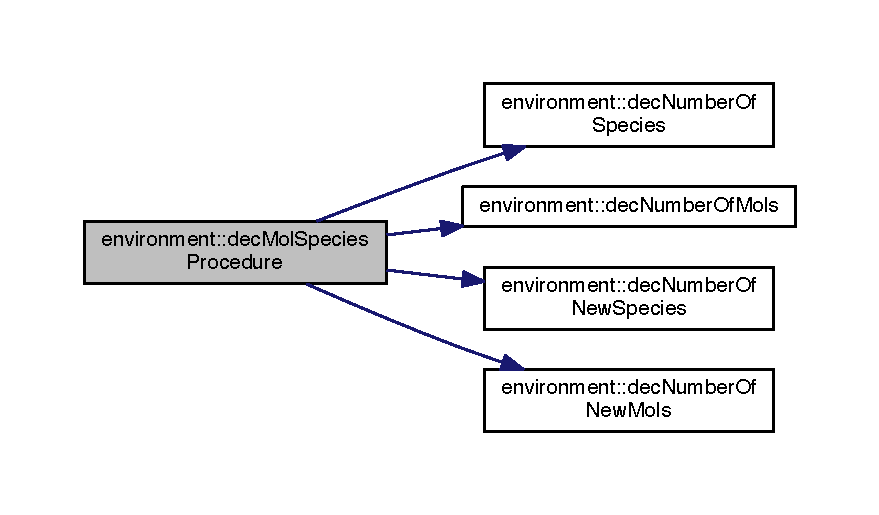
\includegraphics[width=350pt]{a00013_a10fad450cf5ef3a1c7cf75d616105069_cgraph}
\end{center}
\end{figure}


\hypertarget{a00013_aadd057e7038269e6fac314a12a3bf334}{\index{environment@{environment}!dec\+Number\+Of\+Cpx@{dec\+Number\+Of\+Cpx}}
\index{dec\+Number\+Of\+Cpx@{dec\+Number\+Of\+Cpx}!environment@{environment}}
\subsubsection[{dec\+Number\+Of\+Cpx}]{\setlength{\rightskip}{0pt plus 5cm}void environment\+::dec\+Number\+Of\+Cpx (
\begin{DoxyParamCaption}
\item[{{\bf acs\+\_\+int}}]{tmp\+I\+D}
\end{DoxyParamCaption}
)\hspace{0.3cm}{\ttfamily [inline]}}}\label{a00013_aadd057e7038269e6fac314a12a3bf334}


Definition at line 288 of file environment.\+h.



Here is the caller graph for this function\+:\nopagebreak
\begin{figure}[H]
\begin{center}
\leavevmode
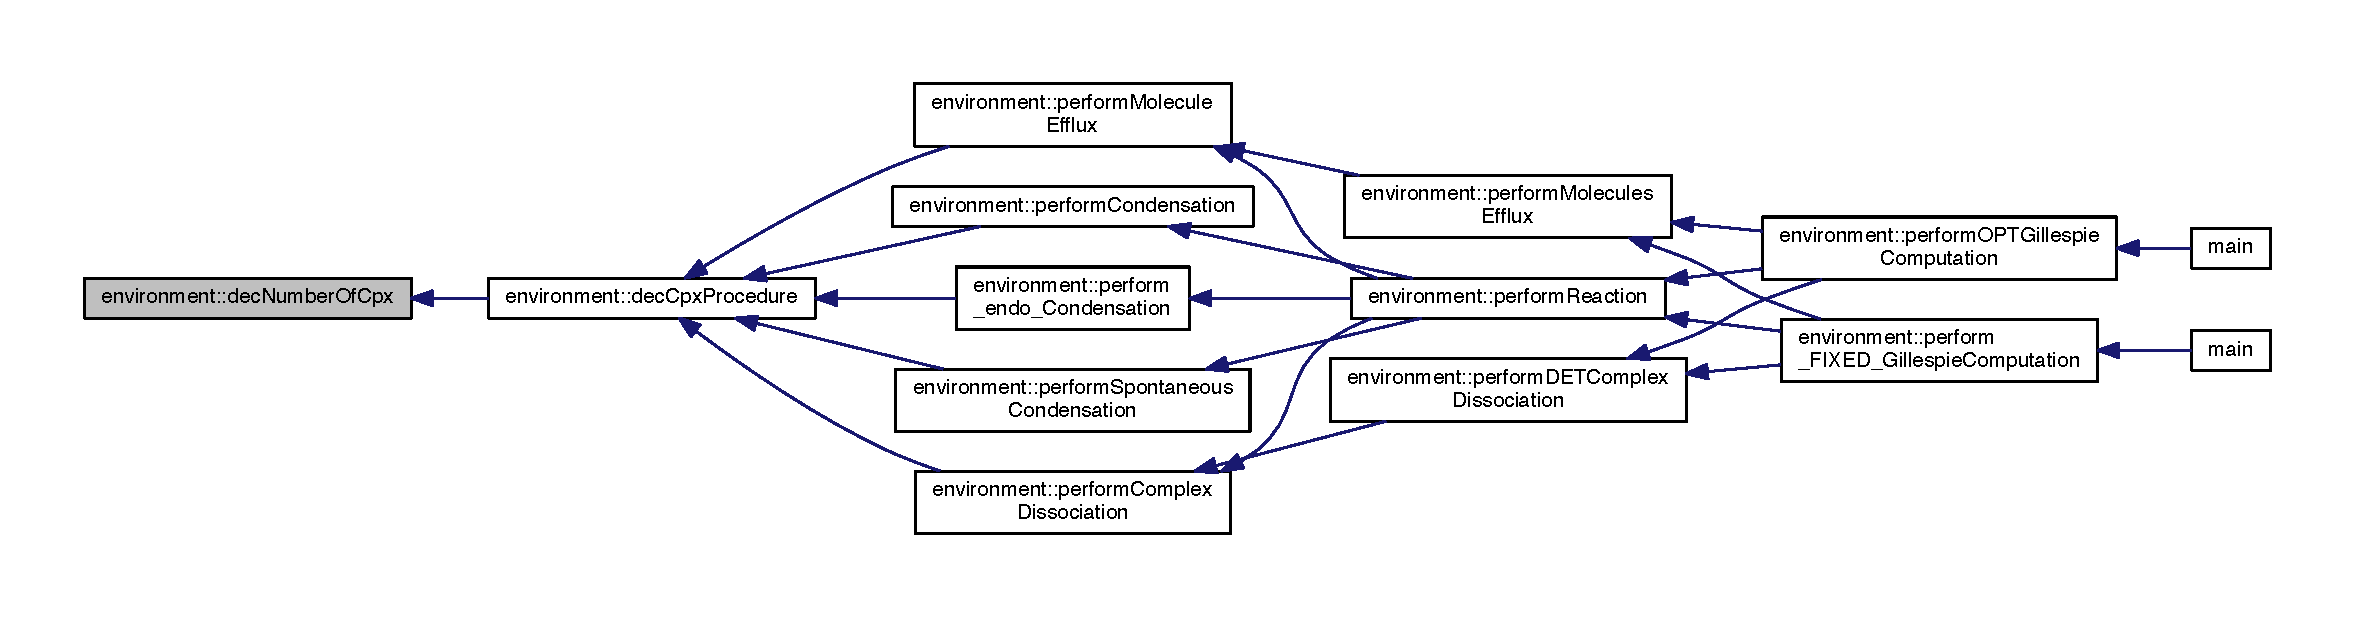
\includegraphics[width=350pt]{a00013_aadd057e7038269e6fac314a12a3bf334_icgraph}
\end{center}
\end{figure}


\hypertarget{a00013_aadd057e7038269e6fac314a12a3bf334}{\index{environment@{environment}!dec\+Number\+Of\+Cpx@{dec\+Number\+Of\+Cpx}}
\index{dec\+Number\+Of\+Cpx@{dec\+Number\+Of\+Cpx}!environment@{environment}}
\subsubsection[{dec\+Number\+Of\+Cpx}]{\setlength{\rightskip}{0pt plus 5cm}void environment\+::dec\+Number\+Of\+Cpx (
\begin{DoxyParamCaption}
\item[{{\bf acs\+\_\+int}}]{tmp\+I\+D}
\end{DoxyParamCaption}
)\hspace{0.3cm}{\ttfamily [inline]}}}\label{a00013_aadd057e7038269e6fac314a12a3bf334}


Definition at line 317 of file environment.\+h.

\hypertarget{a00013_a756dc43b6b47498ba457613749324b15}{\index{environment@{environment}!dec\+Number\+Of\+Cpx\+Mols@{dec\+Number\+Of\+Cpx\+Mols}}
\index{dec\+Number\+Of\+Cpx\+Mols@{dec\+Number\+Of\+Cpx\+Mols}!environment@{environment}}
\subsubsection[{dec\+Number\+Of\+Cpx\+Mols}]{\setlength{\rightskip}{0pt plus 5cm}void environment\+::dec\+Number\+Of\+Cpx\+Mols (
\begin{DoxyParamCaption}
{}
\end{DoxyParamCaption}
)\hspace{0.3cm}{\ttfamily [inline]}}}\label{a00013_a756dc43b6b47498ba457613749324b15}


Definition at line 290 of file environment.\+h.



Here is the caller graph for this function\+:\nopagebreak
\begin{figure}[H]
\begin{center}
\leavevmode
\includegraphics[width=350pt]{a00013_a756dc43b6b47498ba457613749324b15_icgraph}
\end{center}
\end{figure}


\hypertarget{a00013_a756dc43b6b47498ba457613749324b15}{\index{environment@{environment}!dec\+Number\+Of\+Cpx\+Mols@{dec\+Number\+Of\+Cpx\+Mols}}
\index{dec\+Number\+Of\+Cpx\+Mols@{dec\+Number\+Of\+Cpx\+Mols}!environment@{environment}}
\subsubsection[{dec\+Number\+Of\+Cpx\+Mols}]{\setlength{\rightskip}{0pt plus 5cm}void environment\+::dec\+Number\+Of\+Cpx\+Mols (
\begin{DoxyParamCaption}
{}
\end{DoxyParamCaption}
)\hspace{0.3cm}{\ttfamily [inline]}}}\label{a00013_a756dc43b6b47498ba457613749324b15}


Definition at line 319 of file environment.\+h.

\hypertarget{a00013_af042f7904c92fdd239995bebbab2cf60}{\index{environment@{environment}!dec\+Number\+Of\+Mols@{dec\+Number\+Of\+Mols}}
\index{dec\+Number\+Of\+Mols@{dec\+Number\+Of\+Mols}!environment@{environment}}
\subsubsection[{dec\+Number\+Of\+Mols}]{\setlength{\rightskip}{0pt plus 5cm}void environment\+::dec\+Number\+Of\+Mols (
\begin{DoxyParamCaption}
{}
\end{DoxyParamCaption}
)\hspace{0.3cm}{\ttfamily [inline]}}}\label{a00013_af042f7904c92fdd239995bebbab2cf60}


Definition at line 286 of file environment.\+h.



Here is the caller graph for this function\+:\nopagebreak
\begin{figure}[H]
\begin{center}
\leavevmode
\includegraphics[width=350pt]{a00013_af042f7904c92fdd239995bebbab2cf60_icgraph}
\end{center}
\end{figure}


\hypertarget{a00013_af042f7904c92fdd239995bebbab2cf60}{\index{environment@{environment}!dec\+Number\+Of\+Mols@{dec\+Number\+Of\+Mols}}
\index{dec\+Number\+Of\+Mols@{dec\+Number\+Of\+Mols}!environment@{environment}}
\subsubsection[{dec\+Number\+Of\+Mols}]{\setlength{\rightskip}{0pt plus 5cm}void environment\+::dec\+Number\+Of\+Mols (
\begin{DoxyParamCaption}
{}
\end{DoxyParamCaption}
)\hspace{0.3cm}{\ttfamily [inline]}}}\label{a00013_af042f7904c92fdd239995bebbab2cf60}


Definition at line 315 of file environment.\+h.

\hypertarget{a00013_ae9bbd78076706050ced4dd7fb99036f1}{\index{environment@{environment}!dec\+Number\+Of\+New\+Mols@{dec\+Number\+Of\+New\+Mols}}
\index{dec\+Number\+Of\+New\+Mols@{dec\+Number\+Of\+New\+Mols}!environment@{environment}}
\subsubsection[{dec\+Number\+Of\+New\+Mols}]{\setlength{\rightskip}{0pt plus 5cm}void environment\+::dec\+Number\+Of\+New\+Mols (
\begin{DoxyParamCaption}
\item[{{\bf acs\+\_\+int}}]{tmp\+I\+D}
\end{DoxyParamCaption}
)\hspace{0.3cm}{\ttfamily [inline]}}}\label{a00013_ae9bbd78076706050ced4dd7fb99036f1}


Definition at line 295 of file environment.\+h.



Here is the caller graph for this function\+:\nopagebreak
\begin{figure}[H]
\begin{center}
\leavevmode
\includegraphics[width=350pt]{a00013_ae9bbd78076706050ced4dd7fb99036f1_icgraph}
\end{center}
\end{figure}


\hypertarget{a00013_ae9bbd78076706050ced4dd7fb99036f1}{\index{environment@{environment}!dec\+Number\+Of\+New\+Mols@{dec\+Number\+Of\+New\+Mols}}
\index{dec\+Number\+Of\+New\+Mols@{dec\+Number\+Of\+New\+Mols}!environment@{environment}}
\subsubsection[{dec\+Number\+Of\+New\+Mols}]{\setlength{\rightskip}{0pt plus 5cm}void environment\+::dec\+Number\+Of\+New\+Mols (
\begin{DoxyParamCaption}
\item[{{\bf acs\+\_\+int}}]{tmp\+I\+D}
\end{DoxyParamCaption}
)\hspace{0.3cm}{\ttfamily [inline]}}}\label{a00013_ae9bbd78076706050ced4dd7fb99036f1}


Definition at line 324 of file environment.\+h.

\hypertarget{a00013_a5fa52a4f8e73a71fa41d3a1641e50535}{\index{environment@{environment}!dec\+Number\+Of\+New\+Species@{dec\+Number\+Of\+New\+Species}}
\index{dec\+Number\+Of\+New\+Species@{dec\+Number\+Of\+New\+Species}!environment@{environment}}
\subsubsection[{dec\+Number\+Of\+New\+Species}]{\setlength{\rightskip}{0pt plus 5cm}void environment\+::dec\+Number\+Of\+New\+Species (
\begin{DoxyParamCaption}
\item[{{\bf acs\+\_\+int}}]{tmp\+I\+D}
\end{DoxyParamCaption}
)\hspace{0.3cm}{\ttfamily [inline]}}}\label{a00013_a5fa52a4f8e73a71fa41d3a1641e50535}


Definition at line 293 of file environment.\+h.



Here is the caller graph for this function\+:\nopagebreak
\begin{figure}[H]
\begin{center}
\leavevmode
\includegraphics[width=350pt]{a00013_a5fa52a4f8e73a71fa41d3a1641e50535_icgraph}
\end{center}
\end{figure}


\hypertarget{a00013_a5fa52a4f8e73a71fa41d3a1641e50535}{\index{environment@{environment}!dec\+Number\+Of\+New\+Species@{dec\+Number\+Of\+New\+Species}}
\index{dec\+Number\+Of\+New\+Species@{dec\+Number\+Of\+New\+Species}!environment@{environment}}
\subsubsection[{dec\+Number\+Of\+New\+Species}]{\setlength{\rightskip}{0pt plus 5cm}void environment\+::dec\+Number\+Of\+New\+Species (
\begin{DoxyParamCaption}
\item[{{\bf acs\+\_\+int}}]{tmp\+I\+D}
\end{DoxyParamCaption}
)\hspace{0.3cm}{\ttfamily [inline]}}}\label{a00013_a5fa52a4f8e73a71fa41d3a1641e50535}


Definition at line 322 of file environment.\+h.

\hypertarget{a00013_a69a926e0b9bb4f4b29876d0e45b54d84}{\index{environment@{environment}!dec\+Number\+Of\+Species@{dec\+Number\+Of\+Species}}
\index{dec\+Number\+Of\+Species@{dec\+Number\+Of\+Species}!environment@{environment}}
\subsubsection[{dec\+Number\+Of\+Species}]{\setlength{\rightskip}{0pt plus 5cm}void environment\+::dec\+Number\+Of\+Species (
\begin{DoxyParamCaption}
\item[{{\bf acs\+\_\+int}}]{tmp\+I\+D}
\end{DoxyParamCaption}
)\hspace{0.3cm}{\ttfamily [inline]}}}\label{a00013_a69a926e0b9bb4f4b29876d0e45b54d84}


Definition at line 284 of file environment.\+h.



Here is the caller graph for this function\+:\nopagebreak
\begin{figure}[H]
\begin{center}
\leavevmode
\includegraphics[width=350pt]{a00013_a69a926e0b9bb4f4b29876d0e45b54d84_icgraph}
\end{center}
\end{figure}


\hypertarget{a00013_a69a926e0b9bb4f4b29876d0e45b54d84}{\index{environment@{environment}!dec\+Number\+Of\+Species@{dec\+Number\+Of\+Species}}
\index{dec\+Number\+Of\+Species@{dec\+Number\+Of\+Species}!environment@{environment}}
\subsubsection[{dec\+Number\+Of\+Species}]{\setlength{\rightskip}{0pt plus 5cm}void environment\+::dec\+Number\+Of\+Species (
\begin{DoxyParamCaption}
\item[{{\bf acs\+\_\+int}}]{tmp\+I\+D}
\end{DoxyParamCaption}
)\hspace{0.3cm}{\ttfamily [inline]}}}\label{a00013_a69a926e0b9bb4f4b29876d0e45b54d84}


Definition at line 313 of file environment.\+h.

\hypertarget{a00013_a6686b0489ed94f11c4b03c011978f9af}{\index{environment@{environment}!dec\+Overall\+Loaded\+Mols\+Counter@{dec\+Overall\+Loaded\+Mols\+Counter}}
\index{dec\+Overall\+Loaded\+Mols\+Counter@{dec\+Overall\+Loaded\+Mols\+Counter}!environment@{environment}}
\subsubsection[{dec\+Overall\+Loaded\+Mols\+Counter}]{\setlength{\rightskip}{0pt plus 5cm}void environment\+::dec\+Overall\+Loaded\+Mols\+Counter (
\begin{DoxyParamCaption}
{}
\end{DoxyParamCaption}
)\hspace{0.3cm}{\ttfamily [inline]}}}\label{a00013_a6686b0489ed94f11c4b03c011978f9af}


Definition at line 311 of file environment.\+h.



Here is the caller graph for this function\+:\nopagebreak
\begin{figure}[H]
\begin{center}
\leavevmode
\includegraphics[width=350pt]{a00013_a6686b0489ed94f11c4b03c011978f9af_icgraph}
\end{center}
\end{figure}


\hypertarget{a00013_a6686b0489ed94f11c4b03c011978f9af}{\index{environment@{environment}!dec\+Overall\+Loaded\+Mols\+Counter@{dec\+Overall\+Loaded\+Mols\+Counter}}
\index{dec\+Overall\+Loaded\+Mols\+Counter@{dec\+Overall\+Loaded\+Mols\+Counter}!environment@{environment}}
\subsubsection[{dec\+Overall\+Loaded\+Mols\+Counter}]{\setlength{\rightskip}{0pt plus 5cm}void environment\+::dec\+Overall\+Loaded\+Mols\+Counter (
\begin{DoxyParamCaption}
{}
\end{DoxyParamCaption}
)\hspace{0.3cm}{\ttfamily [inline]}}}\label{a00013_a6686b0489ed94f11c4b03c011978f9af}


Definition at line 340 of file environment.\+h.

\hypertarget{a00013_ae7fd21d14f81c4854b3a6163b0278857}{\index{environment@{environment}!dev\+Std@{dev\+Std}}
\index{dev\+Std@{dev\+Std}!environment@{environment}}
\subsubsection[{dev\+Std}]{\setlength{\rightskip}{0pt plus 5cm}bool environment\+::dev\+Std (
\begin{DoxyParamCaption}
{}
\end{DoxyParamCaption}
)}}\label{a00013_ae7fd21d14f81c4854b3a6163b0278857}
Save living species in a file named living\+\_\+species\+\_\+\mbox{[}current\+Sim\mbox{]}.csv. Standard C++ The file is saved in the directory indicated as a second parameter in the run command \begin{DoxyVersion}{Version}
1.\+1 
\end{DoxyVersion}
\begin{DoxyDate}{Date}
2014-\/05-\/11 Save living species total A\+M\+O\+U\+N\+T in a file named living\+Amount\+\_\+\mbox{[}Current\+Gen\mbox{]}\+\_\+\mbox{[}current\+Sim\mbox{]}.csv. The file is saved in the directory indicated as a second parameter in the run command -\/ Standard C++ 
\end{DoxyDate}
\begin{DoxyVersion}{Version}
1.\+1 
\end{DoxyVersion}
\begin{DoxyDate}{Date}
2014-\/05-\/11 Save living species total C\+O\+N\+C\+E\+N\+T\+R\+A\+T\+I\+O\+N in a file named living\+Amount\+\_\+\mbox{[}Current\+Gen\mbox{]}\+\_\+\mbox{[}current\+Sim\mbox{]}.csv. The file is saved in the directory indicated as a second parameter in the run command 
\end{DoxyDate}
\begin{DoxyVersion}{Version}
1.\+1 
\end{DoxyVersion}
\begin{DoxyDate}{Date}
2014-\/05-\/11 
\end{DoxyDate}


Definition at line 7352 of file environment.\+cpp.



Here is the caller graph for this function\+:\nopagebreak
\begin{figure}[H]
\begin{center}
\leavevmode
\includegraphics[width=350pt]{a00013_ae7fd21d14f81c4854b3a6163b0278857_icgraph}
\end{center}
\end{figure}


\hypertarget{a00013_ae7fd21d14f81c4854b3a6163b0278857}{\index{environment@{environment}!dev\+Std@{dev\+Std}}
\index{dev\+Std@{dev\+Std}!environment@{environment}}
\subsubsection[{dev\+Std}]{\setlength{\rightskip}{0pt plus 5cm}bool environment\+::dev\+Std (
\begin{DoxyParamCaption}
{}
\end{DoxyParamCaption}
)}}\label{a00013_ae7fd21d14f81c4854b3a6163b0278857}
\hypertarget{a00013_a4e9b60ec8b05e888cf0e55def03ee906}{\index{environment@{environment}!entropy@{entropy}}
\index{entropy@{entropy}!environment@{environment}}
\subsubsection[{entropy}]{\setlength{\rightskip}{0pt plus 5cm}bool environment\+::entropy (
\begin{DoxyParamCaption}
{}
\end{DoxyParamCaption}
)}}\label{a00013_a4e9b60ec8b05e888cf0e55def03ee906}


Definition at line 7370 of file environment.\+cpp.



Here is the caller graph for this function\+:\nopagebreak
\begin{figure}[H]
\begin{center}
\leavevmode
\includegraphics[width=350pt]{a00013_a4e9b60ec8b05e888cf0e55def03ee906_icgraph}
\end{center}
\end{figure}


\hypertarget{a00013_a4e9b60ec8b05e888cf0e55def03ee906}{\index{environment@{environment}!entropy@{entropy}}
\index{entropy@{entropy}!environment@{environment}}
\subsubsection[{entropy}]{\setlength{\rightskip}{0pt plus 5cm}bool environment\+::entropy (
\begin{DoxyParamCaption}
{}
\end{DoxyParamCaption}
)}}\label{a00013_a4e9b60ec8b05e888cf0e55def03ee906}
\hypertarget{a00013_a14bad649a73246617361f0e1765f49f8}{\index{environment@{environment}!get\+Actual\+Time@{get\+Actual\+Time}}
\index{get\+Actual\+Time@{get\+Actual\+Time}!environment@{environment}}
\subsubsection[{get\+Actual\+Time}]{\setlength{\rightskip}{0pt plus 5cm}{\bf acs\+\_\+double} environment\+::get\+Actual\+Time (
\begin{DoxyParamCaption}
{}
\end{DoxyParamCaption}
) const\hspace{0.3cm}{\ttfamily [inline]}}}\label{a00013_a14bad649a73246617361f0e1765f49f8}


Definition at line 153 of file environment.\+h.



Here is the caller graph for this function\+:\nopagebreak
\begin{figure}[H]
\begin{center}
\leavevmode
\includegraphics[width=350pt]{a00013_a14bad649a73246617361f0e1765f49f8_icgraph}
\end{center}
\end{figure}


\hypertarget{a00013_a14bad649a73246617361f0e1765f49f8}{\index{environment@{environment}!get\+Actual\+Time@{get\+Actual\+Time}}
\index{get\+Actual\+Time@{get\+Actual\+Time}!environment@{environment}}
\subsubsection[{get\+Actual\+Time}]{\setlength{\rightskip}{0pt plus 5cm}{\bf acs\+\_\+double} environment\+::get\+Actual\+Time (
\begin{DoxyParamCaption}
{}
\end{DoxyParamCaption}
) const\hspace{0.3cm}{\ttfamily [inline]}}}\label{a00013_a14bad649a73246617361f0e1765f49f8}


Definition at line 165 of file environment.\+h.

\hypertarget{a00013_a69d18914fe7c8e96b10992668960b83b}{\index{environment@{environment}!get\+A\+D\+P@{get\+A\+D\+P}}
\index{get\+A\+D\+P@{get\+A\+D\+P}!environment@{environment}}
\subsubsection[{get\+A\+D\+P}]{\setlength{\rightskip}{0pt plus 5cm}{\bf acs\+\_\+int} environment\+::get\+A\+D\+P (
\begin{DoxyParamCaption}
{}
\end{DoxyParamCaption}
) const\hspace{0.3cm}{\ttfamily [inline]}}}\label{a00013_a69d18914fe7c8e96b10992668960b83b}


Definition at line 169 of file environment.\+h.

\hypertarget{a00013_a69d18914fe7c8e96b10992668960b83b}{\index{environment@{environment}!get\+A\+D\+P@{get\+A\+D\+P}}
\index{get\+A\+D\+P@{get\+A\+D\+P}!environment@{environment}}
\subsubsection[{get\+A\+D\+P}]{\setlength{\rightskip}{0pt plus 5cm}{\bf acs\+\_\+int} environment\+::get\+A\+D\+P (
\begin{DoxyParamCaption}
{}
\end{DoxyParamCaption}
) const\hspace{0.3cm}{\ttfamily [inline]}}}\label{a00013_a69d18914fe7c8e96b10992668960b83b}


Definition at line 182 of file environment.\+h.

\hypertarget{a00013_add8478cfc878c3aa5a57b2a71357a088}{\index{environment@{environment}!get\+Alphabet@{get\+Alphabet}}
\index{get\+Alphabet@{get\+Alphabet}!environment@{environment}}
\subsubsection[{get\+Alphabet}]{\setlength{\rightskip}{0pt plus 5cm}string environment\+::get\+Alphabet (
\begin{DoxyParamCaption}
{}
\end{DoxyParamCaption}
) const\hspace{0.3cm}{\ttfamily [inline]}}}\label{a00013_add8478cfc878c3aa5a57b2a71357a088}


Definition at line 207 of file environment.\+h.

\hypertarget{a00013_add8478cfc878c3aa5a57b2a71357a088}{\index{environment@{environment}!get\+Alphabet@{get\+Alphabet}}
\index{get\+Alphabet@{get\+Alphabet}!environment@{environment}}
\subsubsection[{get\+Alphabet}]{\setlength{\rightskip}{0pt plus 5cm}string environment\+::get\+Alphabet (
\begin{DoxyParamCaption}
{}
\end{DoxyParamCaption}
) const\hspace{0.3cm}{\ttfamily [inline]}}}\label{a00013_add8478cfc878c3aa5a57b2a71357a088}


Definition at line 224 of file environment.\+h.

\hypertarget{a00013_a02346c5d824e83e0a76dd01f4672ad8b}{\index{environment@{environment}!get\+A\+T\+P@{get\+A\+T\+P}}
\index{get\+A\+T\+P@{get\+A\+T\+P}!environment@{environment}}
\subsubsection[{get\+A\+T\+P}]{\setlength{\rightskip}{0pt plus 5cm}{\bf acs\+\_\+int} environment\+::get\+A\+T\+P (
\begin{DoxyParamCaption}
{}
\end{DoxyParamCaption}
) const\hspace{0.3cm}{\ttfamily [inline]}}}\label{a00013_a02346c5d824e83e0a76dd01f4672ad8b}


Definition at line 170 of file environment.\+h.

\hypertarget{a00013_a02346c5d824e83e0a76dd01f4672ad8b}{\index{environment@{environment}!get\+A\+T\+P@{get\+A\+T\+P}}
\index{get\+A\+T\+P@{get\+A\+T\+P}!environment@{environment}}
\subsubsection[{get\+A\+T\+P}]{\setlength{\rightskip}{0pt plus 5cm}{\bf acs\+\_\+int} environment\+::get\+A\+T\+P (
\begin{DoxyParamCaption}
{}
\end{DoxyParamCaption}
) const\hspace{0.3cm}{\ttfamily [inline]}}}\label{a00013_a02346c5d824e83e0a76dd01f4672ad8b}


Definition at line 183 of file environment.\+h.

\hypertarget{a00013_ab87d94260cc7a7b388deca45fddb6031}{\index{environment@{environment}!get\+Buffer\+Rcts\+Count\+Row@{get\+Buffer\+Rcts\+Count\+Row}}
\index{get\+Buffer\+Rcts\+Count\+Row@{get\+Buffer\+Rcts\+Count\+Row}!environment@{environment}}
\subsubsection[{get\+Buffer\+Rcts\+Count\+Row}]{\setlength{\rightskip}{0pt plus 5cm}{\bf acs\+\_\+int} environment\+::get\+Buffer\+Rcts\+Count\+Row (
\begin{DoxyParamCaption}
{}
\end{DoxyParamCaption}
) const\hspace{0.3cm}{\ttfamily [inline]}}}\label{a00013_ab87d94260cc7a7b388deca45fddb6031}


Definition at line 190 of file environment.\+h.



Here is the caller graph for this function\+:\nopagebreak
\begin{figure}[H]
\begin{center}
\leavevmode
\includegraphics[width=292pt]{a00013_ab87d94260cc7a7b388deca45fddb6031_icgraph}
\end{center}
\end{figure}


\hypertarget{a00013_a8b9a3b5c5a2f86206c5fb124352e366e}{\index{environment@{environment}!get\+Cleavage\+Counter@{get\+Cleavage\+Counter}}
\index{get\+Cleavage\+Counter@{get\+Cleavage\+Counter}!environment@{environment}}
\subsubsection[{get\+Cleavage\+Counter}]{\setlength{\rightskip}{0pt plus 5cm}{\bf acs\+\_\+long\+Int} environment\+::get\+Cleavage\+Counter (
\begin{DoxyParamCaption}
{}
\end{DoxyParamCaption}
) const\hspace{0.3cm}{\ttfamily [inline]}}}\label{a00013_a8b9a3b5c5a2f86206c5fb124352e366e}


Definition at line 226 of file environment.\+h.



Here is the caller graph for this function\+:\nopagebreak
\begin{figure}[H]
\begin{center}
\leavevmode
\includegraphics[width=288pt]{a00013_a8b9a3b5c5a2f86206c5fb124352e366e_icgraph}
\end{center}
\end{figure}


\hypertarget{a00013_a8b9a3b5c5a2f86206c5fb124352e366e}{\index{environment@{environment}!get\+Cleavage\+Counter@{get\+Cleavage\+Counter}}
\index{get\+Cleavage\+Counter@{get\+Cleavage\+Counter}!environment@{environment}}
\subsubsection[{get\+Cleavage\+Counter}]{\setlength{\rightskip}{0pt plus 5cm}{\bf acs\+\_\+long\+Int} environment\+::get\+Cleavage\+Counter (
\begin{DoxyParamCaption}
{}
\end{DoxyParamCaption}
) const\hspace{0.3cm}{\ttfamily [inline]}}}\label{a00013_a8b9a3b5c5a2f86206c5fb124352e366e}


Definition at line 243 of file environment.\+h.

\hypertarget{a00013_a771963196a27d3532cd7af4b98a5a9c5}{\index{environment@{environment}!get\+Cleavage\+K\+C@{get\+Cleavage\+K\+C}}
\index{get\+Cleavage\+K\+C@{get\+Cleavage\+K\+C}!environment@{environment}}
\subsubsection[{get\+Cleavage\+K\+C}]{\setlength{\rightskip}{0pt plus 5cm}{\bf acs\+\_\+double} environment\+::get\+Cleavage\+K\+C (
\begin{DoxyParamCaption}
{}
\end{DoxyParamCaption}
) const\hspace{0.3cm}{\ttfamily [inline]}}}\label{a00013_a771963196a27d3532cd7af4b98a5a9c5}


Definition at line 195 of file environment.\+h.

\hypertarget{a00013_a771963196a27d3532cd7af4b98a5a9c5}{\index{environment@{environment}!get\+Cleavage\+K\+C@{get\+Cleavage\+K\+C}}
\index{get\+Cleavage\+K\+C@{get\+Cleavage\+K\+C}!environment@{environment}}
\subsubsection[{get\+Cleavage\+K\+C}]{\setlength{\rightskip}{0pt plus 5cm}{\bf acs\+\_\+double} environment\+::get\+Cleavage\+K\+C (
\begin{DoxyParamCaption}
{}
\end{DoxyParamCaption}
) const\hspace{0.3cm}{\ttfamily [inline]}}}\label{a00013_a771963196a27d3532cd7af4b98a5a9c5}


Definition at line 212 of file environment.\+h.

\hypertarget{a00013_ac728f6ab012c42fa85a2e2f70df7dc58}{\index{environment@{environment}!get\+Cleav\+Prob@{get\+Cleav\+Prob}}
\index{get\+Cleav\+Prob@{get\+Cleav\+Prob}!environment@{environment}}
\subsubsection[{get\+Cleav\+Prob}]{\setlength{\rightskip}{0pt plus 5cm}{\bf acs\+\_\+double} environment\+::get\+Cleav\+Prob (
\begin{DoxyParamCaption}
{}
\end{DoxyParamCaption}
) const\hspace{0.3cm}{\ttfamily [inline]}}}\label{a00013_ac728f6ab012c42fa85a2e2f70df7dc58}


Definition at line 165 of file environment.\+h.

\hypertarget{a00013_ac728f6ab012c42fa85a2e2f70df7dc58}{\index{environment@{environment}!get\+Cleav\+Prob@{get\+Cleav\+Prob}}
\index{get\+Cleav\+Prob@{get\+Cleav\+Prob}!environment@{environment}}
\subsubsection[{get\+Cleav\+Prob}]{\setlength{\rightskip}{0pt plus 5cm}{\bf acs\+\_\+double} environment\+::get\+Cleav\+Prob (
\begin{DoxyParamCaption}
{}
\end{DoxyParamCaption}
) const\hspace{0.3cm}{\ttfamily [inline]}}}\label{a00013_ac728f6ab012c42fa85a2e2f70df7dc58}


Definition at line 178 of file environment.\+h.

\hypertarget{a00013_ae58bcd60ae01a8ba12f83c1328121c35}{\index{environment@{environment}!get\+Complex\+Deg\+K\+C@{get\+Complex\+Deg\+K\+C}}
\index{get\+Complex\+Deg\+K\+C@{get\+Complex\+Deg\+K\+C}!environment@{environment}}
\subsubsection[{get\+Complex\+Deg\+K\+C}]{\setlength{\rightskip}{0pt plus 5cm}{\bf acs\+\_\+double} environment\+::get\+Complex\+Deg\+K\+C (
\begin{DoxyParamCaption}
{}
\end{DoxyParamCaption}
) const\hspace{0.3cm}{\ttfamily [inline]}}}\label{a00013_ae58bcd60ae01a8ba12f83c1328121c35}


Definition at line 198 of file environment.\+h.

\hypertarget{a00013_ae58bcd60ae01a8ba12f83c1328121c35}{\index{environment@{environment}!get\+Complex\+Deg\+K\+C@{get\+Complex\+Deg\+K\+C}}
\index{get\+Complex\+Deg\+K\+C@{get\+Complex\+Deg\+K\+C}!environment@{environment}}
\subsubsection[{get\+Complex\+Deg\+K\+C}]{\setlength{\rightskip}{0pt plus 5cm}{\bf acs\+\_\+double} environment\+::get\+Complex\+Deg\+K\+C (
\begin{DoxyParamCaption}
{}
\end{DoxyParamCaption}
) const\hspace{0.3cm}{\ttfamily [inline]}}}\label{a00013_ae58bcd60ae01a8ba12f83c1328121c35}


Definition at line 215 of file environment.\+h.

\hypertarget{a00013_aa88b64fa5005973926a121f1aa46770d}{\index{environment@{environment}!get\+Complex\+I\+D@{get\+Complex\+I\+D}}
\index{get\+Complex\+I\+D@{get\+Complex\+I\+D}!environment@{environment}}
\subsubsection[{get\+Complex\+I\+D}]{\setlength{\rightskip}{0pt plus 5cm}{\bf acs\+\_\+long\+Int} environment\+::get\+Complex\+I\+D (
\begin{DoxyParamCaption}
\item[{string}]{sequence, }
\item[{{\bf acs\+\_\+int}}]{cutting\+Point}
\end{DoxyParamCaption}
)}}\label{a00013_aa88b64fa5005973926a121f1aa46770d}
This function searches the complex with sequence and cutting point identical to the parameters and returns (if complex is found) the Complex\+I\+D. If not found, it returns the new I\+D for creating the complex (size of species' array). \begin{DoxyVersion}{Version}
1.\+0 
\end{DoxyVersion}
\begin{DoxyDate}{Date}
2014-\/04-\/14 
\end{DoxyDate}

\begin{DoxyParams}{Parameters}
{\em string} & sequence \\
\hline
{\em acs\+\_\+int} & cutting\+Point \\
\hline
\end{DoxyParams}


Definition at line 6151 of file environment.\+cpp.



Here is the caller graph for this function\+:\nopagebreak
\begin{figure}[H]
\begin{center}
\leavevmode
\includegraphics[width=350pt]{a00013_aa88b64fa5005973926a121f1aa46770d_icgraph}
\end{center}
\end{figure}


\hypertarget{a00013_abf3168adf05ff9fa6bab4e34b387f0a6}{\index{environment@{environment}!get\+Complex\+K\+C@{get\+Complex\+K\+C}}
\index{get\+Complex\+K\+C@{get\+Complex\+K\+C}!environment@{environment}}
\subsubsection[{get\+Complex\+K\+C}]{\setlength{\rightskip}{0pt plus 5cm}{\bf acs\+\_\+double} environment\+::get\+Complex\+K\+C (
\begin{DoxyParamCaption}
{}
\end{DoxyParamCaption}
) const\hspace{0.3cm}{\ttfamily [inline]}}}\label{a00013_abf3168adf05ff9fa6bab4e34b387f0a6}


Definition at line 196 of file environment.\+h.

\hypertarget{a00013_abf3168adf05ff9fa6bab4e34b387f0a6}{\index{environment@{environment}!get\+Complex\+K\+C@{get\+Complex\+K\+C}}
\index{get\+Complex\+K\+C@{get\+Complex\+K\+C}!environment@{environment}}
\subsubsection[{get\+Complex\+K\+C}]{\setlength{\rightskip}{0pt plus 5cm}{\bf acs\+\_\+double} environment\+::get\+Complex\+K\+C (
\begin{DoxyParamCaption}
{}
\end{DoxyParamCaption}
) const\hspace{0.3cm}{\ttfamily [inline]}}}\label{a00013_abf3168adf05ff9fa6bab4e34b387f0a6}


Definition at line 213 of file environment.\+h.

\hypertarget{a00013_a0fc62131bf552c2a995c7ddc461828cd}{\index{environment@{environment}!get\+Condensation\+Counter@{get\+Condensation\+Counter}}
\index{get\+Condensation\+Counter@{get\+Condensation\+Counter}!environment@{environment}}
\subsubsection[{get\+Condensation\+Counter}]{\setlength{\rightskip}{0pt plus 5cm}{\bf acs\+\_\+long\+Int} environment\+::get\+Condensation\+Counter (
\begin{DoxyParamCaption}
{}
\end{DoxyParamCaption}
) const\hspace{0.3cm}{\ttfamily [inline]}}}\label{a00013_a0fc62131bf552c2a995c7ddc461828cd}


Definition at line 228 of file environment.\+h.



Here is the caller graph for this function\+:\nopagebreak
\begin{figure}[H]
\begin{center}
\leavevmode
\includegraphics[width=308pt]{a00013_a0fc62131bf552c2a995c7ddc461828cd_icgraph}
\end{center}
\end{figure}


\hypertarget{a00013_a0fc62131bf552c2a995c7ddc461828cd}{\index{environment@{environment}!get\+Condensation\+Counter@{get\+Condensation\+Counter}}
\index{get\+Condensation\+Counter@{get\+Condensation\+Counter}!environment@{environment}}
\subsubsection[{get\+Condensation\+Counter}]{\setlength{\rightskip}{0pt plus 5cm}{\bf acs\+\_\+long\+Int} environment\+::get\+Condensation\+Counter (
\begin{DoxyParamCaption}
{}
\end{DoxyParamCaption}
) const\hspace{0.3cm}{\ttfamily [inline]}}}\label{a00013_a0fc62131bf552c2a995c7ddc461828cd}


Definition at line 245 of file environment.\+h.

\hypertarget{a00013_a7ac1b69dd38107d5c40339563969d09f}{\index{environment@{environment}!get\+Condensation\+K\+C@{get\+Condensation\+K\+C}}
\index{get\+Condensation\+K\+C@{get\+Condensation\+K\+C}!environment@{environment}}
\subsubsection[{get\+Condensation\+K\+C}]{\setlength{\rightskip}{0pt plus 5cm}{\bf acs\+\_\+double} environment\+::get\+Condensation\+K\+C (
\begin{DoxyParamCaption}
{}
\end{DoxyParamCaption}
) const\hspace{0.3cm}{\ttfamily [inline]}}}\label{a00013_a7ac1b69dd38107d5c40339563969d09f}


Definition at line 197 of file environment.\+h.

\hypertarget{a00013_a7ac1b69dd38107d5c40339563969d09f}{\index{environment@{environment}!get\+Condensation\+K\+C@{get\+Condensation\+K\+C}}
\index{get\+Condensation\+K\+C@{get\+Condensation\+K\+C}!environment@{environment}}
\subsubsection[{get\+Condensation\+K\+C}]{\setlength{\rightskip}{0pt plus 5cm}{\bf acs\+\_\+double} environment\+::get\+Condensation\+K\+C (
\begin{DoxyParamCaption}
{}
\end{DoxyParamCaption}
) const\hspace{0.3cm}{\ttfamily [inline]}}}\label{a00013_a7ac1b69dd38107d5c40339563969d09f}


Definition at line 214 of file environment.\+h.

\hypertarget{a00013_abf2f63b22c52e17f6089f098651584b8}{\index{environment@{environment}!get\+Cpx\+Diss\+Counter@{get\+Cpx\+Diss\+Counter}}
\index{get\+Cpx\+Diss\+Counter@{get\+Cpx\+Diss\+Counter}!environment@{environment}}
\subsubsection[{get\+Cpx\+Diss\+Counter}]{\setlength{\rightskip}{0pt plus 5cm}{\bf acs\+\_\+long\+Int} environment\+::get\+Cpx\+Diss\+Counter (
\begin{DoxyParamCaption}
{}
\end{DoxyParamCaption}
) const\hspace{0.3cm}{\ttfamily [inline]}}}\label{a00013_abf2f63b22c52e17f6089f098651584b8}


Definition at line 231 of file environment.\+h.



Here is the caller graph for this function\+:\nopagebreak
\begin{figure}[H]
\begin{center}
\leavevmode
\includegraphics[width=318pt]{a00013_abf2f63b22c52e17f6089f098651584b8_icgraph}
\end{center}
\end{figure}


\hypertarget{a00013_abf2f63b22c52e17f6089f098651584b8}{\index{environment@{environment}!get\+Cpx\+Diss\+Counter@{get\+Cpx\+Diss\+Counter}}
\index{get\+Cpx\+Diss\+Counter@{get\+Cpx\+Diss\+Counter}!environment@{environment}}
\subsubsection[{get\+Cpx\+Diss\+Counter}]{\setlength{\rightskip}{0pt plus 5cm}{\bf acs\+\_\+long\+Int} environment\+::get\+Cpx\+Diss\+Counter (
\begin{DoxyParamCaption}
{}
\end{DoxyParamCaption}
) const\hspace{0.3cm}{\ttfamily [inline]}}}\label{a00013_abf2f63b22c52e17f6089f098651584b8}


Definition at line 248 of file environment.\+h.

\hypertarget{a00013_a5d72675f37c3936c58d27480613a9ab6}{\index{environment@{environment}!get\+Cpx\+Form\+Counter@{get\+Cpx\+Form\+Counter}}
\index{get\+Cpx\+Form\+Counter@{get\+Cpx\+Form\+Counter}!environment@{environment}}
\subsubsection[{get\+Cpx\+Form\+Counter}]{\setlength{\rightskip}{0pt plus 5cm}{\bf acs\+\_\+long\+Int} environment\+::get\+Cpx\+Form\+Counter (
\begin{DoxyParamCaption}
{}
\end{DoxyParamCaption}
) const\hspace{0.3cm}{\ttfamily [inline]}}}\label{a00013_a5d72675f37c3936c58d27480613a9ab6}


Definition at line 230 of file environment.\+h.



Here is the caller graph for this function\+:\nopagebreak
\begin{figure}[H]
\begin{center}
\leavevmode
\includegraphics[width=322pt]{a00013_a5d72675f37c3936c58d27480613a9ab6_icgraph}
\end{center}
\end{figure}


\hypertarget{a00013_a5d72675f37c3936c58d27480613a9ab6}{\index{environment@{environment}!get\+Cpx\+Form\+Counter@{get\+Cpx\+Form\+Counter}}
\index{get\+Cpx\+Form\+Counter@{get\+Cpx\+Form\+Counter}!environment@{environment}}
\subsubsection[{get\+Cpx\+Form\+Counter}]{\setlength{\rightskip}{0pt plus 5cm}{\bf acs\+\_\+long\+Int} environment\+::get\+Cpx\+Form\+Counter (
\begin{DoxyParamCaption}
{}
\end{DoxyParamCaption}
) const\hspace{0.3cm}{\ttfamily [inline]}}}\label{a00013_a5d72675f37c3936c58d27480613a9ab6}


Definition at line 247 of file environment.\+h.

\hypertarget{a00013_a0851e3481e6fec7f4feef126d5a6704c}{\index{environment@{environment}!get\+Current\+Attempts@{get\+Current\+Attempts}}
\index{get\+Current\+Attempts@{get\+Current\+Attempts}!environment@{environment}}
\subsubsection[{get\+Current\+Attempts}]{\setlength{\rightskip}{0pt plus 5cm}{\bf acs\+\_\+int} environment\+::get\+Current\+Attempts (
\begin{DoxyParamCaption}
{}
\end{DoxyParamCaption}
) const\hspace{0.3cm}{\ttfamily [inline]}}}\label{a00013_a0851e3481e6fec7f4feef126d5a6704c}


Definition at line 158 of file environment.\+h.



Here is the caller graph for this function\+:\nopagebreak
\begin{figure}[H]
\begin{center}
\leavevmode
\includegraphics[width=318pt]{a00013_a0851e3481e6fec7f4feef126d5a6704c_icgraph}
\end{center}
\end{figure}


\hypertarget{a00013_a0851e3481e6fec7f4feef126d5a6704c}{\index{environment@{environment}!get\+Current\+Attempts@{get\+Current\+Attempts}}
\index{get\+Current\+Attempts@{get\+Current\+Attempts}!environment@{environment}}
\subsubsection[{get\+Current\+Attempts}]{\setlength{\rightskip}{0pt plus 5cm}{\bf acs\+\_\+int} environment\+::get\+Current\+Attempts (
\begin{DoxyParamCaption}
{}
\end{DoxyParamCaption}
) const\hspace{0.3cm}{\ttfamily [inline]}}}\label{a00013_a0851e3481e6fec7f4feef126d5a6704c}


Definition at line 170 of file environment.\+h.

\hypertarget{a00013_a2de42381b0b9cba889bbb95c1456cfe5}{\index{environment@{environment}!get\+Debug\+Level@{get\+Debug\+Level}}
\index{get\+Debug\+Level@{get\+Debug\+Level}!environment@{environment}}
\subsubsection[{get\+Debug\+Level}]{\setlength{\rightskip}{0pt plus 5cm}int environment\+::get\+Debug\+Level (
\begin{DoxyParamCaption}
{}
\end{DoxyParamCaption}
) const\hspace{0.3cm}{\ttfamily [inline]}}}\label{a00013_a2de42381b0b9cba889bbb95c1456cfe5}


Definition at line 218 of file environment.\+h.



Here is the caller graph for this function\+:\nopagebreak
\begin{figure}[H]
\begin{center}
\leavevmode
\includegraphics[width=298pt]{a00013_a2de42381b0b9cba889bbb95c1456cfe5_icgraph}
\end{center}
\end{figure}


\hypertarget{a00013_a2de42381b0b9cba889bbb95c1456cfe5}{\index{environment@{environment}!get\+Debug\+Level@{get\+Debug\+Level}}
\index{get\+Debug\+Level@{get\+Debug\+Level}!environment@{environment}}
\subsubsection[{get\+Debug\+Level}]{\setlength{\rightskip}{0pt plus 5cm}int environment\+::get\+Debug\+Level (
\begin{DoxyParamCaption}
{}
\end{DoxyParamCaption}
) const\hspace{0.3cm}{\ttfamily [inline]}}}\label{a00013_a2de42381b0b9cba889bbb95c1456cfe5}


Definition at line 235 of file environment.\+h.

\hypertarget{a00013_a46193e153bd5dcc37fb35346cb7fd971}{\index{environment@{environment}!get\+Diffusion\+Contribute@{get\+Diffusion\+Contribute}}
\index{get\+Diffusion\+Contribute@{get\+Diffusion\+Contribute}!environment@{environment}}
\subsubsection[{get\+Diffusion\+Contribute}]{\setlength{\rightskip}{0pt plus 5cm}{\bf acs\+\_\+double} environment\+::get\+Diffusion\+Contribute (
\begin{DoxyParamCaption}
{}
\end{DoxyParamCaption}
) const\hspace{0.3cm}{\ttfamily [inline]}}}\label{a00013_a46193e153bd5dcc37fb35346cb7fd971}


Definition at line 204 of file environment.\+h.

\hypertarget{a00013_a46193e153bd5dcc37fb35346cb7fd971}{\index{environment@{environment}!get\+Diffusion\+Contribute@{get\+Diffusion\+Contribute}}
\index{get\+Diffusion\+Contribute@{get\+Diffusion\+Contribute}!environment@{environment}}
\subsubsection[{get\+Diffusion\+Contribute}]{\setlength{\rightskip}{0pt plus 5cm}{\bf acs\+\_\+double} environment\+::get\+Diffusion\+Contribute (
\begin{DoxyParamCaption}
{}
\end{DoxyParamCaption}
) const\hspace{0.3cm}{\ttfamily [inline]}}}\label{a00013_a46193e153bd5dcc37fb35346cb7fd971}


Definition at line 221 of file environment.\+h.

\hypertarget{a00013_aa2ded3c5ba8c4ce41ee86399dc616d4a}{\index{environment@{environment}!get\+Endo\+Cleavage\+Counter@{get\+Endo\+Cleavage\+Counter}}
\index{get\+Endo\+Cleavage\+Counter@{get\+Endo\+Cleavage\+Counter}!environment@{environment}}
\subsubsection[{get\+Endo\+Cleavage\+Counter}]{\setlength{\rightskip}{0pt plus 5cm}{\bf acs\+\_\+long\+Int} environment\+::get\+Endo\+Cleavage\+Counter (
\begin{DoxyParamCaption}
{}
\end{DoxyParamCaption}
) const\hspace{0.3cm}{\ttfamily [inline]}}}\label{a00013_aa2ded3c5ba8c4ce41ee86399dc616d4a}


Definition at line 227 of file environment.\+h.



Here is the caller graph for this function\+:\nopagebreak
\begin{figure}[H]
\begin{center}
\leavevmode
\includegraphics[width=312pt]{a00013_aa2ded3c5ba8c4ce41ee86399dc616d4a_icgraph}
\end{center}
\end{figure}


\hypertarget{a00013_aa2ded3c5ba8c4ce41ee86399dc616d4a}{\index{environment@{environment}!get\+Endo\+Cleavage\+Counter@{get\+Endo\+Cleavage\+Counter}}
\index{get\+Endo\+Cleavage\+Counter@{get\+Endo\+Cleavage\+Counter}!environment@{environment}}
\subsubsection[{get\+Endo\+Cleavage\+Counter}]{\setlength{\rightskip}{0pt plus 5cm}{\bf acs\+\_\+long\+Int} environment\+::get\+Endo\+Cleavage\+Counter (
\begin{DoxyParamCaption}
{}
\end{DoxyParamCaption}
) const\hspace{0.3cm}{\ttfamily [inline]}}}\label{a00013_aa2ded3c5ba8c4ce41ee86399dc616d4a}


Definition at line 244 of file environment.\+h.

\hypertarget{a00013_aaa23d550cfa37344dd3bb4d5767e6ea0}{\index{environment@{environment}!get\+Endo\+Condensation\+Counter@{get\+Endo\+Condensation\+Counter}}
\index{get\+Endo\+Condensation\+Counter@{get\+Endo\+Condensation\+Counter}!environment@{environment}}
\subsubsection[{get\+Endo\+Condensation\+Counter}]{\setlength{\rightskip}{0pt plus 5cm}{\bf acs\+\_\+long\+Int} environment\+::get\+Endo\+Condensation\+Counter (
\begin{DoxyParamCaption}
{}
\end{DoxyParamCaption}
) const\hspace{0.3cm}{\ttfamily [inline]}}}\label{a00013_aaa23d550cfa37344dd3bb4d5767e6ea0}


Definition at line 229 of file environment.\+h.



Here is the caller graph for this function\+:\nopagebreak
\begin{figure}[H]
\begin{center}
\leavevmode
\includegraphics[width=330pt]{a00013_aaa23d550cfa37344dd3bb4d5767e6ea0_icgraph}
\end{center}
\end{figure}


\hypertarget{a00013_aaa23d550cfa37344dd3bb4d5767e6ea0}{\index{environment@{environment}!get\+Endo\+Condensation\+Counter@{get\+Endo\+Condensation\+Counter}}
\index{get\+Endo\+Condensation\+Counter@{get\+Endo\+Condensation\+Counter}!environment@{environment}}
\subsubsection[{get\+Endo\+Condensation\+Counter}]{\setlength{\rightskip}{0pt plus 5cm}{\bf acs\+\_\+long\+Int} environment\+::get\+Endo\+Condensation\+Counter (
\begin{DoxyParamCaption}
{}
\end{DoxyParamCaption}
) const\hspace{0.3cm}{\ttfamily [inline]}}}\label{a00013_aaa23d550cfa37344dd3bb4d5767e6ea0}


Definition at line 246 of file environment.\+h.

\hypertarget{a00013_ab463a460de102c79c1044ab8a2c176ae}{\index{environment@{environment}!get\+Energy@{get\+Energy}}
\index{get\+Energy@{get\+Energy}!environment@{environment}}
\subsubsection[{get\+Energy}]{\setlength{\rightskip}{0pt plus 5cm}{\bf acs\+\_\+int} environment\+::get\+Energy (
\begin{DoxyParamCaption}
{}
\end{DoxyParamCaption}
) const\hspace{0.3cm}{\ttfamily [inline]}}}\label{a00013_ab463a460de102c79c1044ab8a2c176ae}


Definition at line 167 of file environment.\+h.



Here is the caller graph for this function\+:\nopagebreak
\begin{figure}[H]
\begin{center}
\leavevmode
\includegraphics[width=350pt]{a00013_ab463a460de102c79c1044ab8a2c176ae_icgraph}
\end{center}
\end{figure}


\hypertarget{a00013_ab463a460de102c79c1044ab8a2c176ae}{\index{environment@{environment}!get\+Energy@{get\+Energy}}
\index{get\+Energy@{get\+Energy}!environment@{environment}}
\subsubsection[{get\+Energy}]{\setlength{\rightskip}{0pt plus 5cm}{\bf acs\+\_\+int} environment\+::get\+Energy (
\begin{DoxyParamCaption}
{}
\end{DoxyParamCaption}
) const\hspace{0.3cm}{\ttfamily [inline]}}}\label{a00013_ab463a460de102c79c1044ab8a2c176ae}


Definition at line 180 of file environment.\+h.

\hypertarget{a00013_adf74cb3545d95a7965e3a18cfc98cebe}{\index{environment@{environment}!get\+File\+Amount\+Saving\+Interval@{get\+File\+Amount\+Saving\+Interval}}
\index{get\+File\+Amount\+Saving\+Interval@{get\+File\+Amount\+Saving\+Interval}!environment@{environment}}
\subsubsection[{get\+File\+Amount\+Saving\+Interval}]{\setlength{\rightskip}{0pt plus 5cm}{\bf acs\+\_\+double} environment\+::get\+File\+Amount\+Saving\+Interval (
\begin{DoxyParamCaption}
{}
\end{DoxyParamCaption}
) const\hspace{0.3cm}{\ttfamily [inline]}}}\label{a00013_adf74cb3545d95a7965e3a18cfc98cebe}


Definition at line 174 of file environment.\+h.



Here is the caller graph for this function\+:\nopagebreak
\begin{figure}[H]
\begin{center}
\leavevmode
\includegraphics[width=296pt]{a00013_adf74cb3545d95a7965e3a18cfc98cebe_icgraph}
\end{center}
\end{figure}


\hypertarget{a00013_a77e995bee54ab4e09f165a857a7b0272}{\index{environment@{environment}!get\+File\+Times\+Saving\+Interval@{get\+File\+Times\+Saving\+Interval}}
\index{get\+File\+Times\+Saving\+Interval@{get\+File\+Times\+Saving\+Interval}!environment@{environment}}
\subsubsection[{get\+File\+Times\+Saving\+Interval}]{\setlength{\rightskip}{0pt plus 5cm}{\bf acs\+\_\+double} environment\+::get\+File\+Times\+Saving\+Interval (
\begin{DoxyParamCaption}
{}
\end{DoxyParamCaption}
) const\hspace{0.3cm}{\ttfamily [inline]}}}\label{a00013_a77e995bee54ab4e09f165a857a7b0272}


Definition at line 160 of file environment.\+h.



Here is the caller graph for this function\+:\nopagebreak
\begin{figure}[H]
\begin{center}
\leavevmode
\includegraphics[width=350pt]{a00013_a77e995bee54ab4e09f165a857a7b0272_icgraph}
\end{center}
\end{figure}


\hypertarget{a00013_a77e995bee54ab4e09f165a857a7b0272}{\index{environment@{environment}!get\+File\+Times\+Saving\+Interval@{get\+File\+Times\+Saving\+Interval}}
\index{get\+File\+Times\+Saving\+Interval@{get\+File\+Times\+Saving\+Interval}!environment@{environment}}
\subsubsection[{get\+File\+Times\+Saving\+Interval}]{\setlength{\rightskip}{0pt plus 5cm}{\bf acs\+\_\+double} environment\+::get\+File\+Times\+Saving\+Interval (
\begin{DoxyParamCaption}
{}
\end{DoxyParamCaption}
) const\hspace{0.3cm}{\ttfamily [inline]}}}\label{a00013_a77e995bee54ab4e09f165a857a7b0272}


Definition at line 173 of file environment.\+h.

\hypertarget{a00013_af4cba1a1f9c1c0106241ca5338b7906d}{\index{environment@{environment}!getgillespie\+Entropy@{getgillespie\+Entropy}}
\index{getgillespie\+Entropy@{getgillespie\+Entropy}!environment@{environment}}
\subsubsection[{getgillespie\+Entropy}]{\setlength{\rightskip}{0pt plus 5cm}{\bf acs\+\_\+double} environment\+::getgillespie\+Entropy (
\begin{DoxyParamCaption}
{}
\end{DoxyParamCaption}
) const\hspace{0.3cm}{\ttfamily [inline]}}}\label{a00013_af4cba1a1f9c1c0106241ca5338b7906d}


Definition at line 180 of file environment.\+h.



Here is the caller graph for this function\+:\nopagebreak
\begin{figure}[H]
\begin{center}
\leavevmode
\includegraphics[width=282pt]{a00013_af4cba1a1f9c1c0106241ca5338b7906d_icgraph}
\end{center}
\end{figure}


\hypertarget{a00013_af4cba1a1f9c1c0106241ca5338b7906d}{\index{environment@{environment}!getgillespie\+Entropy@{getgillespie\+Entropy}}
\index{getgillespie\+Entropy@{getgillespie\+Entropy}!environment@{environment}}
\subsubsection[{getgillespie\+Entropy}]{\setlength{\rightskip}{0pt plus 5cm}{\bf acs\+\_\+double} environment\+::getgillespie\+Entropy (
\begin{DoxyParamCaption}
{}
\end{DoxyParamCaption}
) const\hspace{0.3cm}{\ttfamily [inline]}}}\label{a00013_af4cba1a1f9c1c0106241ca5338b7906d}


Definition at line 195 of file environment.\+h.

\hypertarget{a00013_a389a70abe42c7652c9511b7ed3b974c0}{\index{environment@{environment}!get\+Gillespie\+Mean@{get\+Gillespie\+Mean}}
\index{get\+Gillespie\+Mean@{get\+Gillespie\+Mean}!environment@{environment}}
\subsubsection[{get\+Gillespie\+Mean}]{\setlength{\rightskip}{0pt plus 5cm}{\bf acs\+\_\+double} environment\+::get\+Gillespie\+Mean (
\begin{DoxyParamCaption}
{}
\end{DoxyParamCaption}
) const\hspace{0.3cm}{\ttfamily [inline]}}}\label{a00013_a389a70abe42c7652c9511b7ed3b974c0}


Definition at line 178 of file environment.\+h.



Here is the caller graph for this function\+:\nopagebreak
\begin{figure}[H]
\begin{center}
\leavevmode
\includegraphics[width=308pt]{a00013_a389a70abe42c7652c9511b7ed3b974c0_icgraph}
\end{center}
\end{figure}


\hypertarget{a00013_a389a70abe42c7652c9511b7ed3b974c0}{\index{environment@{environment}!get\+Gillespie\+Mean@{get\+Gillespie\+Mean}}
\index{get\+Gillespie\+Mean@{get\+Gillespie\+Mean}!environment@{environment}}
\subsubsection[{get\+Gillespie\+Mean}]{\setlength{\rightskip}{0pt plus 5cm}{\bf acs\+\_\+double} environment\+::get\+Gillespie\+Mean (
\begin{DoxyParamCaption}
{}
\end{DoxyParamCaption}
) const\hspace{0.3cm}{\ttfamily [inline]}}}\label{a00013_a389a70abe42c7652c9511b7ed3b974c0}


Definition at line 193 of file environment.\+h.

\hypertarget{a00013_a41d9f79794b74845f2d00b4c0affea02}{\index{environment@{environment}!getgillespie\+S\+D@{getgillespie\+S\+D}}
\index{getgillespie\+S\+D@{getgillespie\+S\+D}!environment@{environment}}
\subsubsection[{getgillespie\+S\+D}]{\setlength{\rightskip}{0pt plus 5cm}{\bf acs\+\_\+double} environment\+::getgillespie\+S\+D (
\begin{DoxyParamCaption}
{}
\end{DoxyParamCaption}
) const\hspace{0.3cm}{\ttfamily [inline]}}}\label{a00013_a41d9f79794b74845f2d00b4c0affea02}


Definition at line 179 of file environment.\+h.



Here is the caller graph for this function\+:\nopagebreak
\begin{figure}[H]
\begin{center}
\leavevmode
\includegraphics[width=296pt]{a00013_a41d9f79794b74845f2d00b4c0affea02_icgraph}
\end{center}
\end{figure}


\hypertarget{a00013_a41d9f79794b74845f2d00b4c0affea02}{\index{environment@{environment}!getgillespie\+S\+D@{getgillespie\+S\+D}}
\index{getgillespie\+S\+D@{getgillespie\+S\+D}!environment@{environment}}
\subsubsection[{getgillespie\+S\+D}]{\setlength{\rightskip}{0pt plus 5cm}{\bf acs\+\_\+double} environment\+::getgillespie\+S\+D (
\begin{DoxyParamCaption}
{}
\end{DoxyParamCaption}
) const\hspace{0.3cm}{\ttfamily [inline]}}}\label{a00013_a41d9f79794b74845f2d00b4c0affea02}


Definition at line 194 of file environment.\+h.

\hypertarget{a00013_a6f0b4481779cd12dbcd8155916c7d703}{\index{environment@{environment}!get\+Influx@{get\+Influx}}
\index{get\+Influx@{get\+Influx}!environment@{environment}}
\subsubsection[{get\+Influx}]{\setlength{\rightskip}{0pt plus 5cm}{\bf acs\+\_\+double} environment\+::get\+Influx (
\begin{DoxyParamCaption}
{}
\end{DoxyParamCaption}
) const\hspace{0.3cm}{\ttfamily [inline]}}}\label{a00013_a6f0b4481779cd12dbcd8155916c7d703}


Definition at line 205 of file environment.\+h.



Here is the caller graph for this function\+:\nopagebreak
\begin{figure}[H]
\begin{center}
\leavevmode
\includegraphics[width=350pt]{a00013_a6f0b4481779cd12dbcd8155916c7d703_icgraph}
\end{center}
\end{figure}


\hypertarget{a00013_a6f0b4481779cd12dbcd8155916c7d703}{\index{environment@{environment}!get\+Influx@{get\+Influx}}
\index{get\+Influx@{get\+Influx}!environment@{environment}}
\subsubsection[{get\+Influx}]{\setlength{\rightskip}{0pt plus 5cm}{\bf acs\+\_\+double} environment\+::get\+Influx (
\begin{DoxyParamCaption}
{}
\end{DoxyParamCaption}
) const\hspace{0.3cm}{\ttfamily [inline]}}}\label{a00013_a6f0b4481779cd12dbcd8155916c7d703}


Definition at line 222 of file environment.\+h.

\hypertarget{a00013_a6557765370b636bc7d4e02288b444c0e}{\index{environment@{environment}!get\+K\+\_\+spont\+\_\+ass@{get\+K\+\_\+spont\+\_\+ass}}
\index{get\+K\+\_\+spont\+\_\+ass@{get\+K\+\_\+spont\+\_\+ass}!environment@{environment}}
\subsubsection[{get\+K\+\_\+spont\+\_\+ass}]{\setlength{\rightskip}{0pt plus 5cm}{\bf acs\+\_\+double} environment\+::get\+K\+\_\+spont\+\_\+ass (
\begin{DoxyParamCaption}
{}
\end{DoxyParamCaption}
) const\hspace{0.3cm}{\ttfamily [inline]}}}\label{a00013_a6557765370b636bc7d4e02288b444c0e}


Definition at line 193 of file environment.\+h.

\hypertarget{a00013_a6557765370b636bc7d4e02288b444c0e}{\index{environment@{environment}!get\+K\+\_\+spont\+\_\+ass@{get\+K\+\_\+spont\+\_\+ass}}
\index{get\+K\+\_\+spont\+\_\+ass@{get\+K\+\_\+spont\+\_\+ass}!environment@{environment}}
\subsubsection[{get\+K\+\_\+spont\+\_\+ass}]{\setlength{\rightskip}{0pt plus 5cm}{\bf acs\+\_\+double} environment\+::get\+K\+\_\+spont\+\_\+ass (
\begin{DoxyParamCaption}
{}
\end{DoxyParamCaption}
) const\hspace{0.3cm}{\ttfamily [inline]}}}\label{a00013_a6557765370b636bc7d4e02288b444c0e}


Definition at line 210 of file environment.\+h.

\hypertarget{a00013_a2c6ca24592b5feab891e43233c581711}{\index{environment@{environment}!get\+K\+\_\+spont\+\_\+diss@{get\+K\+\_\+spont\+\_\+diss}}
\index{get\+K\+\_\+spont\+\_\+diss@{get\+K\+\_\+spont\+\_\+diss}!environment@{environment}}
\subsubsection[{get\+K\+\_\+spont\+\_\+diss}]{\setlength{\rightskip}{0pt plus 5cm}{\bf acs\+\_\+double} environment\+::get\+K\+\_\+spont\+\_\+diss (
\begin{DoxyParamCaption}
{}
\end{DoxyParamCaption}
) const\hspace{0.3cm}{\ttfamily [inline]}}}\label{a00013_a2c6ca24592b5feab891e43233c581711}


Definition at line 192 of file environment.\+h.

\hypertarget{a00013_a2c6ca24592b5feab891e43233c581711}{\index{environment@{environment}!get\+K\+\_\+spont\+\_\+diss@{get\+K\+\_\+spont\+\_\+diss}}
\index{get\+K\+\_\+spont\+\_\+diss@{get\+K\+\_\+spont\+\_\+diss}!environment@{environment}}
\subsubsection[{get\+K\+\_\+spont\+\_\+diss}]{\setlength{\rightskip}{0pt plus 5cm}{\bf acs\+\_\+double} environment\+::get\+K\+\_\+spont\+\_\+diss (
\begin{DoxyParamCaption}
{}
\end{DoxyParamCaption}
) const\hspace{0.3cm}{\ttfamily [inline]}}}\label{a00013_a2c6ca24592b5feab891e43233c581711}


Definition at line 209 of file environment.\+h.

\hypertarget{a00013_aa862f1f98c6060747d6f1f30377671ff}{\index{environment@{environment}!get\+Kass@{get\+Kass}}
\index{get\+Kass@{get\+Kass}!environment@{environment}}
\subsubsection[{get\+Kass}]{\setlength{\rightskip}{0pt plus 5cm}{\bf acs\+\_\+double} environment\+::get\+Kass (
\begin{DoxyParamCaption}
{}
\end{DoxyParamCaption}
) const\hspace{0.3cm}{\ttfamily [inline]}}}\label{a00013_aa862f1f98c6060747d6f1f30377671ff}


Definition at line 187 of file environment.\+h.



Here is the caller graph for this function\+:\nopagebreak
\begin{figure}[H]
\begin{center}
\leavevmode
\includegraphics[width=350pt]{a00013_aa862f1f98c6060747d6f1f30377671ff_icgraph}
\end{center}
\end{figure}


\hypertarget{a00013_aa862f1f98c6060747d6f1f30377671ff}{\index{environment@{environment}!get\+Kass@{get\+Kass}}
\index{get\+Kass@{get\+Kass}!environment@{environment}}
\subsubsection[{get\+Kass}]{\setlength{\rightskip}{0pt plus 5cm}{\bf acs\+\_\+double} environment\+::get\+Kass (
\begin{DoxyParamCaption}
{}
\end{DoxyParamCaption}
) const\hspace{0.3cm}{\ttfamily [inline]}}}\label{a00013_aa862f1f98c6060747d6f1f30377671ff}


Definition at line 204 of file environment.\+h.

\hypertarget{a00013_ac62c6b719db59d5829e3cc451b237f44}{\index{environment@{environment}!get\+Kcpx@{get\+Kcpx}}
\index{get\+Kcpx@{get\+Kcpx}!environment@{environment}}
\subsubsection[{get\+Kcpx}]{\setlength{\rightskip}{0pt plus 5cm}{\bf acs\+\_\+double} environment\+::get\+Kcpx (
\begin{DoxyParamCaption}
{}
\end{DoxyParamCaption}
) const\hspace{0.3cm}{\ttfamily [inline]}}}\label{a00013_ac62c6b719db59d5829e3cc451b237f44}


Definition at line 188 of file environment.\+h.

\hypertarget{a00013_ac62c6b719db59d5829e3cc451b237f44}{\index{environment@{environment}!get\+Kcpx@{get\+Kcpx}}
\index{get\+Kcpx@{get\+Kcpx}!environment@{environment}}
\subsubsection[{get\+Kcpx}]{\setlength{\rightskip}{0pt plus 5cm}{\bf acs\+\_\+double} environment\+::get\+Kcpx (
\begin{DoxyParamCaption}
{}
\end{DoxyParamCaption}
) const\hspace{0.3cm}{\ttfamily [inline]}}}\label{a00013_ac62c6b719db59d5829e3cc451b237f44}


Definition at line 205 of file environment.\+h.

\hypertarget{a00013_a9091c4a0fe31f6d5f5330e7ebff297a3}{\index{environment@{environment}!get\+Kcpx\+Diss@{get\+Kcpx\+Diss}}
\index{get\+Kcpx\+Diss@{get\+Kcpx\+Diss}!environment@{environment}}
\subsubsection[{get\+Kcpx\+Diss}]{\setlength{\rightskip}{0pt plus 5cm}{\bf acs\+\_\+double} environment\+::get\+Kcpx\+Diss (
\begin{DoxyParamCaption}
{}
\end{DoxyParamCaption}
) const\hspace{0.3cm}{\ttfamily [inline]}}}\label{a00013_a9091c4a0fe31f6d5f5330e7ebff297a3}


Definition at line 189 of file environment.\+h.

\hypertarget{a00013_a9091c4a0fe31f6d5f5330e7ebff297a3}{\index{environment@{environment}!get\+Kcpx\+Diss@{get\+Kcpx\+Diss}}
\index{get\+Kcpx\+Diss@{get\+Kcpx\+Diss}!environment@{environment}}
\subsubsection[{get\+Kcpx\+Diss}]{\setlength{\rightskip}{0pt plus 5cm}{\bf acs\+\_\+double} environment\+::get\+Kcpx\+Diss (
\begin{DoxyParamCaption}
{}
\end{DoxyParamCaption}
) const\hspace{0.3cm}{\ttfamily [inline]}}}\label{a00013_a9091c4a0fe31f6d5f5330e7ebff297a3}


Definition at line 206 of file environment.\+h.

\hypertarget{a00013_ab429d2057ee1092bf210c29e70153f75}{\index{environment@{environment}!get\+Kdiss@{get\+Kdiss}}
\index{get\+Kdiss@{get\+Kdiss}!environment@{environment}}
\subsubsection[{get\+Kdiss}]{\setlength{\rightskip}{0pt plus 5cm}{\bf acs\+\_\+double} environment\+::get\+Kdiss (
\begin{DoxyParamCaption}
{}
\end{DoxyParamCaption}
) const\hspace{0.3cm}{\ttfamily [inline]}}}\label{a00013_ab429d2057ee1092bf210c29e70153f75}


Definition at line 186 of file environment.\+h.



Here is the caller graph for this function\+:\nopagebreak
\begin{figure}[H]
\begin{center}
\leavevmode
\includegraphics[width=350pt]{a00013_ab429d2057ee1092bf210c29e70153f75_icgraph}
\end{center}
\end{figure}


\hypertarget{a00013_ab429d2057ee1092bf210c29e70153f75}{\index{environment@{environment}!get\+Kdiss@{get\+Kdiss}}
\index{get\+Kdiss@{get\+Kdiss}!environment@{environment}}
\subsubsection[{get\+Kdiss}]{\setlength{\rightskip}{0pt plus 5cm}{\bf acs\+\_\+double} environment\+::get\+Kdiss (
\begin{DoxyParamCaption}
{}
\end{DoxyParamCaption}
) const\hspace{0.3cm}{\ttfamily [inline]}}}\label{a00013_ab429d2057ee1092bf210c29e70153f75}


Definition at line 203 of file environment.\+h.

\hypertarget{a00013_a4c163b36e84cd8406aff4ab5d220a251}{\index{environment@{environment}!get\+Kirrad@{get\+Kirrad}}
\index{get\+Kirrad@{get\+Kirrad}!environment@{environment}}
\subsubsection[{get\+Kirrad}]{\setlength{\rightskip}{0pt plus 5cm}{\bf acs\+\_\+double} environment\+::get\+Kirrad (
\begin{DoxyParamCaption}
{}
\end{DoxyParamCaption}
) const\hspace{0.3cm}{\ttfamily [inline]}}}\label{a00013_a4c163b36e84cd8406aff4ab5d220a251}


Definition at line 191 of file environment.\+h.

\hypertarget{a00013_a4c163b36e84cd8406aff4ab5d220a251}{\index{environment@{environment}!get\+Kirrad@{get\+Kirrad}}
\index{get\+Kirrad@{get\+Kirrad}!environment@{environment}}
\subsubsection[{get\+Kirrad}]{\setlength{\rightskip}{0pt plus 5cm}{\bf acs\+\_\+double} environment\+::get\+Kirrad (
\begin{DoxyParamCaption}
{}
\end{DoxyParamCaption}
) const\hspace{0.3cm}{\ttfamily [inline]}}}\label{a00013_a4c163b36e84cd8406aff4ab5d220a251}


Definition at line 208 of file environment.\+h.

\hypertarget{a00013_a7615c746521a592ff1ab2d0793b14d89}{\index{environment@{environment}!get\+Knrg@{get\+Knrg}}
\index{get\+Knrg@{get\+Knrg}!environment@{environment}}
\subsubsection[{get\+Knrg}]{\setlength{\rightskip}{0pt plus 5cm}{\bf acs\+\_\+double} environment\+::get\+Knrg (
\begin{DoxyParamCaption}
{}
\end{DoxyParamCaption}
) const\hspace{0.3cm}{\ttfamily [inline]}}}\label{a00013_a7615c746521a592ff1ab2d0793b14d89}


Definition at line 190 of file environment.\+h.

\hypertarget{a00013_a7615c746521a592ff1ab2d0793b14d89}{\index{environment@{environment}!get\+Knrg@{get\+Knrg}}
\index{get\+Knrg@{get\+Knrg}!environment@{environment}}
\subsubsection[{get\+Knrg}]{\setlength{\rightskip}{0pt plus 5cm}{\bf acs\+\_\+double} environment\+::get\+Knrg (
\begin{DoxyParamCaption}
{}
\end{DoxyParamCaption}
) const\hspace{0.3cm}{\ttfamily [inline]}}}\label{a00013_a7615c746521a592ff1ab2d0793b14d89}


Definition at line 207 of file environment.\+h.

\hypertarget{a00013_a984f79e5f89b774b65db901899687ac0}{\index{environment@{environment}!get\+Last\+Firing\+Disk\+Species\+I\+D@{get\+Last\+Firing\+Disk\+Species\+I\+D}}
\index{get\+Last\+Firing\+Disk\+Species\+I\+D@{get\+Last\+Firing\+Disk\+Species\+I\+D}!environment@{environment}}
\subsubsection[{get\+Last\+Firing\+Disk\+Species\+I\+D}]{\setlength{\rightskip}{0pt plus 5cm}{\bf acs\+\_\+int} environment\+::get\+Last\+Firing\+Disk\+Species\+I\+D (
\begin{DoxyParamCaption}
{}
\end{DoxyParamCaption}
) const\hspace{0.3cm}{\ttfamily [inline]}}}\label{a00013_a984f79e5f89b774b65db901899687ac0}


Definition at line 161 of file environment.\+h.



Here is the caller graph for this function\+:\nopagebreak
\begin{figure}[H]
\begin{center}
\leavevmode
\includegraphics[width=350pt]{a00013_a984f79e5f89b774b65db901899687ac0_icgraph}
\end{center}
\end{figure}


\hypertarget{a00013_a984f79e5f89b774b65db901899687ac0}{\index{environment@{environment}!get\+Last\+Firing\+Disk\+Species\+I\+D@{get\+Last\+Firing\+Disk\+Species\+I\+D}}
\index{get\+Last\+Firing\+Disk\+Species\+I\+D@{get\+Last\+Firing\+Disk\+Species\+I\+D}!environment@{environment}}
\subsubsection[{get\+Last\+Firing\+Disk\+Species\+I\+D}]{\setlength{\rightskip}{0pt plus 5cm}{\bf acs\+\_\+int} environment\+::get\+Last\+Firing\+Disk\+Species\+I\+D (
\begin{DoxyParamCaption}
{}
\end{DoxyParamCaption}
) const\hspace{0.3cm}{\ttfamily [inline]}}}\label{a00013_a984f79e5f89b774b65db901899687ac0}


Definition at line 175 of file environment.\+h.

\hypertarget{a00013_ae626b961a53eeb5e08b4190da235e8dd}{\index{environment@{environment}!get\+M\+A\+Xattempts@{get\+M\+A\+Xattempts}}
\index{get\+M\+A\+Xattempts@{get\+M\+A\+Xattempts}!environment@{environment}}
\subsubsection[{get\+M\+A\+Xattempts}]{\setlength{\rightskip}{0pt plus 5cm}{\bf acs\+\_\+int} environment\+::get\+M\+A\+Xattempts (
\begin{DoxyParamCaption}
{}
\end{DoxyParamCaption}
) const\hspace{0.3cm}{\ttfamily [inline]}}}\label{a00013_ae626b961a53eeb5e08b4190da235e8dd}


Definition at line 157 of file environment.\+h.



Here is the caller graph for this function\+:\nopagebreak
\begin{figure}[H]
\begin{center}
\leavevmode
\includegraphics[width=306pt]{a00013_ae626b961a53eeb5e08b4190da235e8dd_icgraph}
\end{center}
\end{figure}


\hypertarget{a00013_ae626b961a53eeb5e08b4190da235e8dd}{\index{environment@{environment}!get\+M\+A\+Xattempts@{get\+M\+A\+Xattempts}}
\index{get\+M\+A\+Xattempts@{get\+M\+A\+Xattempts}!environment@{environment}}
\subsubsection[{get\+M\+A\+Xattempts}]{\setlength{\rightskip}{0pt plus 5cm}{\bf acs\+\_\+int} environment\+::get\+M\+A\+Xattempts (
\begin{DoxyParamCaption}
{}
\end{DoxyParamCaption}
) const\hspace{0.3cm}{\ttfamily [inline]}}}\label{a00013_ae626b961a53eeb5e08b4190da235e8dd}


Definition at line 169 of file environment.\+h.

\hypertarget{a00013_af2b482132fc3ab299118f7a894bd53a2}{\index{environment@{environment}!get\+M\+A\+Xhours@{get\+M\+A\+Xhours}}
\index{get\+M\+A\+Xhours@{get\+M\+A\+Xhours}!environment@{environment}}
\subsubsection[{get\+M\+A\+Xhours}]{\setlength{\rightskip}{0pt plus 5cm}{\bf acs\+\_\+double} environment\+::get\+M\+A\+Xhours (
\begin{DoxyParamCaption}
{}
\end{DoxyParamCaption}
) const\hspace{0.3cm}{\ttfamily [inline]}}}\label{a00013_af2b482132fc3ab299118f7a894bd53a2}


Definition at line 156 of file environment.\+h.



Here is the caller graph for this function\+:\nopagebreak
\begin{figure}[H]
\begin{center}
\leavevmode
\includegraphics[width=292pt]{a00013_af2b482132fc3ab299118f7a894bd53a2_icgraph}
\end{center}
\end{figure}


\hypertarget{a00013_af2b482132fc3ab299118f7a894bd53a2}{\index{environment@{environment}!get\+M\+A\+Xhours@{get\+M\+A\+Xhours}}
\index{get\+M\+A\+Xhours@{get\+M\+A\+Xhours}!environment@{environment}}
\subsubsection[{get\+M\+A\+Xhours}]{\setlength{\rightskip}{0pt plus 5cm}{\bf acs\+\_\+double} environment\+::get\+M\+A\+Xhours (
\begin{DoxyParamCaption}
{}
\end{DoxyParamCaption}
) const\hspace{0.3cm}{\ttfamily [inline]}}}\label{a00013_af2b482132fc3ab299118f7a894bd53a2}


Definition at line 168 of file environment.\+h.

\hypertarget{a00013_a4c58b3ce555f04f009bcfb7bbc2b0000}{\index{environment@{environment}!get\+Max\+L\+Out@{get\+Max\+L\+Out}}
\index{get\+Max\+L\+Out@{get\+Max\+L\+Out}!environment@{environment}}
\subsubsection[{get\+Max\+L\+Out}]{\setlength{\rightskip}{0pt plus 5cm}{\bf acs\+\_\+int} environment\+::get\+Max\+L\+Out (
\begin{DoxyParamCaption}
{}
\end{DoxyParamCaption}
) const\hspace{0.3cm}{\ttfamily [inline]}}}\label{a00013_a4c58b3ce555f04f009bcfb7bbc2b0000}


Definition at line 200 of file environment.\+h.

\hypertarget{a00013_a4c58b3ce555f04f009bcfb7bbc2b0000}{\index{environment@{environment}!get\+Max\+L\+Out@{get\+Max\+L\+Out}}
\index{get\+Max\+L\+Out@{get\+Max\+L\+Out}!environment@{environment}}
\subsubsection[{get\+Max\+L\+Out}]{\setlength{\rightskip}{0pt plus 5cm}{\bf acs\+\_\+int} environment\+::get\+Max\+L\+Out (
\begin{DoxyParamCaption}
{}
\end{DoxyParamCaption}
) const\hspace{0.3cm}{\ttfamily [inline]}}}\label{a00013_a4c58b3ce555f04f009bcfb7bbc2b0000}


Definition at line 217 of file environment.\+h.

\hypertarget{a00013_aca760caf9354f541020c1db58490b18f}{\index{environment@{environment}!get\+Max\+Non\+Catalytic\+Length@{get\+Max\+Non\+Catalytic\+Length}}
\index{get\+Max\+Non\+Catalytic\+Length@{get\+Max\+Non\+Catalytic\+Length}!environment@{environment}}
\subsubsection[{get\+Max\+Non\+Catalytic\+Length}]{\setlength{\rightskip}{0pt plus 5cm}{\bf acs\+\_\+int} environment\+::get\+Max\+Non\+Catalytic\+Length (
\begin{DoxyParamCaption}
{}
\end{DoxyParamCaption}
) const\hspace{0.3cm}{\ttfamily [inline]}}}\label{a00013_aca760caf9354f541020c1db58490b18f}


Definition at line 163 of file environment.\+h.

\hypertarget{a00013_aca760caf9354f541020c1db58490b18f}{\index{environment@{environment}!get\+Max\+Non\+Catalytic\+Length@{get\+Max\+Non\+Catalytic\+Length}}
\index{get\+Max\+Non\+Catalytic\+Length@{get\+Max\+Non\+Catalytic\+Length}!environment@{environment}}
\subsubsection[{get\+Max\+Non\+Catalytic\+Length}]{\setlength{\rightskip}{0pt plus 5cm}{\bf acs\+\_\+int} environment\+::get\+Max\+Non\+Catalytic\+Length (
\begin{DoxyParamCaption}
{}
\end{DoxyParamCaption}
) const\hspace{0.3cm}{\ttfamily [inline]}}}\label{a00013_aca760caf9354f541020c1db58490b18f}


Definition at line 176 of file environment.\+h.

\hypertarget{a00013_a4ed6ad35297e718398fb42a2b9dbe4ae}{\index{environment@{environment}!get\+Molecule\+Decay\+K\+C@{get\+Molecule\+Decay\+K\+C}}
\index{get\+Molecule\+Decay\+K\+C@{get\+Molecule\+Decay\+K\+C}!environment@{environment}}
\subsubsection[{get\+Molecule\+Decay\+K\+C}]{\setlength{\rightskip}{0pt plus 5cm}{\bf acs\+\_\+double} environment\+::get\+Molecule\+Decay\+K\+C (
\begin{DoxyParamCaption}
{}
\end{DoxyParamCaption}
) const\hspace{0.3cm}{\ttfamily [inline]}}}\label{a00013_a4ed6ad35297e718398fb42a2b9dbe4ae}


Definition at line 199 of file environment.\+h.

\hypertarget{a00013_a4ed6ad35297e718398fb42a2b9dbe4ae}{\index{environment@{environment}!get\+Molecule\+Decay\+K\+C@{get\+Molecule\+Decay\+K\+C}}
\index{get\+Molecule\+Decay\+K\+C@{get\+Molecule\+Decay\+K\+C}!environment@{environment}}
\subsubsection[{get\+Molecule\+Decay\+K\+C}]{\setlength{\rightskip}{0pt plus 5cm}{\bf acs\+\_\+double} environment\+::get\+Molecule\+Decay\+K\+C (
\begin{DoxyParamCaption}
{}
\end{DoxyParamCaption}
) const\hspace{0.3cm}{\ttfamily [inline]}}}\label{a00013_a4ed6ad35297e718398fb42a2b9dbe4ae}


Definition at line 216 of file environment.\+h.

\hypertarget{a00013_adb12eb52af74ea1fdfe0cd195109fe83}{\index{environment@{environment}!get\+Molecules\+Population@{get\+Molecules\+Population}}
\index{get\+Molecules\+Population@{get\+Molecules\+Population}!environment@{environment}}
\subsubsection[{get\+Molecules\+Population}]{\setlength{\rightskip}{0pt plus 5cm}vector$<${\bf species}$>$ environment\+::get\+Molecules\+Population (
\begin{DoxyParamCaption}
{}
\end{DoxyParamCaption}
) const\hspace{0.3cm}{\ttfamily [inline]}}}\label{a00013_adb12eb52af74ea1fdfe0cd195109fe83}


Definition at line 210 of file environment.\+h.

\hypertarget{a00013_adb12eb52af74ea1fdfe0cd195109fe83}{\index{environment@{environment}!get\+Molecules\+Population@{get\+Molecules\+Population}}
\index{get\+Molecules\+Population@{get\+Molecules\+Population}!environment@{environment}}
\subsubsection[{get\+Molecules\+Population}]{\setlength{\rightskip}{0pt plus 5cm}vector$<${\bf species}$>$ environment\+::get\+Molecules\+Population (
\begin{DoxyParamCaption}
{}
\end{DoxyParamCaption}
) const\hspace{0.3cm}{\ttfamily [inline]}}}\label{a00013_adb12eb52af74ea1fdfe0cd195109fe83}


Definition at line 227 of file environment.\+h.

\hypertarget{a00013_a5a2ee72147144e7a04f4b363f1cc0914}{\index{environment@{environment}!get\+Mols@{get\+Mols}}
\index{get\+Mols@{get\+Mols}!environment@{environment}}
\subsubsection[{get\+Mols}]{\setlength{\rightskip}{0pt plus 5cm}{\bf acs\+\_\+long\+Int} environment\+::get\+Mols (
\begin{DoxyParamCaption}
{}
\end{DoxyParamCaption}
) const\hspace{0.3cm}{\ttfamily [inline]}}}\label{a00013_a5a2ee72147144e7a04f4b363f1cc0914}


Definition at line 171 of file environment.\+h.



Here is the caller graph for this function\+:\nopagebreak
\begin{figure}[H]
\begin{center}
\leavevmode
\includegraphics[width=266pt]{a00013_a5a2ee72147144e7a04f4b363f1cc0914_icgraph}
\end{center}
\end{figure}


\hypertarget{a00013_a5a2ee72147144e7a04f4b363f1cc0914}{\index{environment@{environment}!get\+Mols@{get\+Mols}}
\index{get\+Mols@{get\+Mols}!environment@{environment}}
\subsubsection[{get\+Mols}]{\setlength{\rightskip}{0pt plus 5cm}{\bf acs\+\_\+long\+Int} environment\+::get\+Mols (
\begin{DoxyParamCaption}
{}
\end{DoxyParamCaption}
) const\hspace{0.3cm}{\ttfamily [inline]}}}\label{a00013_a5a2ee72147144e7a04f4b363f1cc0914}


Definition at line 184 of file environment.\+h.

\hypertarget{a00013_a5f6c40cbf788d58db588dc6280f0174f}{\index{environment@{environment}!get\+Ncpx@{get\+Ncpx}}
\index{get\+Ncpx@{get\+Ncpx}!environment@{environment}}
\subsubsection[{get\+Ncpx}]{\setlength{\rightskip}{0pt plus 5cm}{\bf acs\+\_\+long\+Int} environment\+::get\+Ncpx (
\begin{DoxyParamCaption}
{}
\end{DoxyParamCaption}
) const\hspace{0.3cm}{\ttfamily [inline]}}}\label{a00013_a5f6c40cbf788d58db588dc6280f0174f}


Definition at line 175 of file environment.\+h.



Here is the caller graph for this function\+:\nopagebreak
\begin{figure}[H]
\begin{center}
\leavevmode
\includegraphics[width=268pt]{a00013_a5f6c40cbf788d58db588dc6280f0174f_icgraph}
\end{center}
\end{figure}


\hypertarget{a00013_a5f6c40cbf788d58db588dc6280f0174f}{\index{environment@{environment}!get\+Ncpx@{get\+Ncpx}}
\index{get\+Ncpx@{get\+Ncpx}!environment@{environment}}
\subsubsection[{get\+Ncpx}]{\setlength{\rightskip}{0pt plus 5cm}{\bf acs\+\_\+long\+Int} environment\+::get\+Ncpx (
\begin{DoxyParamCaption}
{}
\end{DoxyParamCaption}
) const\hspace{0.3cm}{\ttfamily [inline]}}}\label{a00013_a5f6c40cbf788d58db588dc6280f0174f}


Definition at line 188 of file environment.\+h.

\hypertarget{a00013_a39bb98a336b69f25479b8f82b9928bd3}{\index{environment@{environment}!get\+Ncpx\+Mols@{get\+Ncpx\+Mols}}
\index{get\+Ncpx\+Mols@{get\+Ncpx\+Mols}!environment@{environment}}
\subsubsection[{get\+Ncpx\+Mols}]{\setlength{\rightskip}{0pt plus 5cm}{\bf acs\+\_\+long\+Int} environment\+::get\+Ncpx\+Mols (
\begin{DoxyParamCaption}
{}
\end{DoxyParamCaption}
) const\hspace{0.3cm}{\ttfamily [inline]}}}\label{a00013_a39bb98a336b69f25479b8f82b9928bd3}


Definition at line 176 of file environment.\+h.



Here is the caller graph for this function\+:\nopagebreak
\begin{figure}[H]
\begin{center}
\leavevmode
\includegraphics[width=290pt]{a00013_a39bb98a336b69f25479b8f82b9928bd3_icgraph}
\end{center}
\end{figure}


\hypertarget{a00013_a39bb98a336b69f25479b8f82b9928bd3}{\index{environment@{environment}!get\+Ncpx\+Mols@{get\+Ncpx\+Mols}}
\index{get\+Ncpx\+Mols@{get\+Ncpx\+Mols}!environment@{environment}}
\subsubsection[{get\+Ncpx\+Mols}]{\setlength{\rightskip}{0pt plus 5cm}{\bf acs\+\_\+long\+Int} environment\+::get\+Ncpx\+Mols (
\begin{DoxyParamCaption}
{}
\end{DoxyParamCaption}
) const\hspace{0.3cm}{\ttfamily [inline]}}}\label{a00013_a39bb98a336b69f25479b8f82b9928bd3}


Definition at line 189 of file environment.\+h.

\hypertarget{a00013_a57e1eb6043a54fbebd2ac01ebdac9fa1}{\index{environment@{environment}!get\+New\+Mols@{get\+New\+Mols}}
\index{get\+New\+Mols@{get\+New\+Mols}!environment@{environment}}
\subsubsection[{get\+New\+Mols}]{\setlength{\rightskip}{0pt plus 5cm}{\bf acs\+\_\+long\+Int} environment\+::get\+New\+Mols (
\begin{DoxyParamCaption}
{}
\end{DoxyParamCaption}
) const\hspace{0.3cm}{\ttfamily [inline]}}}\label{a00013_a57e1eb6043a54fbebd2ac01ebdac9fa1}


Definition at line 172 of file environment.\+h.



Here is the caller graph for this function\+:\nopagebreak
\begin{figure}[H]
\begin{center}
\leavevmode
\includegraphics[width=286pt]{a00013_a57e1eb6043a54fbebd2ac01ebdac9fa1_icgraph}
\end{center}
\end{figure}


\hypertarget{a00013_acae65ac60e1d746dc3063ae7948b684e}{\index{environment@{environment}!get\+New\+Mols@{get\+New\+Mols}}
\index{get\+New\+Mols@{get\+New\+Mols}!environment@{environment}}
\subsubsection[{get\+New\+Mols}]{\setlength{\rightskip}{0pt plus 5cm}{\bf acs\+\_\+long\+Int} environment\+::get\+New\+Mols (
\begin{DoxyParamCaption}
{}
\end{DoxyParamCaption}
)}}\label{a00013_acae65ac60e1d746dc3063ae7948b684e}
This function returns the number of new molecules \begin{DoxyVersion}{Version}
1.\+0 
\end{DoxyVersion}
\begin{DoxyDate}{Date}
2014-\/05-\/13 
\end{DoxyDate}


Definition at line 6115 of file environment.\+cpp.



Here is the call graph for this function\+:\nopagebreak
\begin{figure}[H]
\begin{center}
\leavevmode
\includegraphics[width=350pt]{a00013_acae65ac60e1d746dc3063ae7948b684e_cgraph}
\end{center}
\end{figure}


\hypertarget{a00013_afad68362d5f4ec0689941e3c1b92c2e8}{\index{environment@{environment}!get\+Ngen@{get\+Ngen}}
\index{get\+Ngen@{get\+Ngen}!environment@{environment}}
\subsubsection[{get\+Ngen}]{\setlength{\rightskip}{0pt plus 5cm}{\bf acs\+\_\+int} environment\+::get\+Ngen (
\begin{DoxyParamCaption}
{}
\end{DoxyParamCaption}
) const\hspace{0.3cm}{\ttfamily [inline]}}}\label{a00013_afad68362d5f4ec0689941e3c1b92c2e8}


Definition at line 151 of file environment.\+h.



Here is the caller graph for this function\+:\nopagebreak
\begin{figure}[H]
\begin{center}
\leavevmode
\includegraphics[width=270pt]{a00013_afad68362d5f4ec0689941e3c1b92c2e8_icgraph}
\end{center}
\end{figure}


\hypertarget{a00013_afad68362d5f4ec0689941e3c1b92c2e8}{\index{environment@{environment}!get\+Ngen@{get\+Ngen}}
\index{get\+Ngen@{get\+Ngen}!environment@{environment}}
\subsubsection[{get\+Ngen}]{\setlength{\rightskip}{0pt plus 5cm}{\bf acs\+\_\+int} environment\+::get\+Ngen (
\begin{DoxyParamCaption}
{}
\end{DoxyParamCaption}
) const\hspace{0.3cm}{\ttfamily [inline]}}}\label{a00013_afad68362d5f4ec0689941e3c1b92c2e8}


Definition at line 163 of file environment.\+h.

\hypertarget{a00013_a4a2b21d139acc93ae0fdf29c8b025cce}{\index{environment@{environment}!get\+Nnew\+Species@{get\+Nnew\+Species}}
\index{get\+Nnew\+Species@{get\+Nnew\+Species}!environment@{environment}}
\subsubsection[{get\+Nnew\+Species}]{\setlength{\rightskip}{0pt plus 5cm}{\bf acs\+\_\+long\+Int} environment\+::get\+Nnew\+Species (
\begin{DoxyParamCaption}
{}
\end{DoxyParamCaption}
) const\hspace{0.3cm}{\ttfamily [inline]}}}\label{a00013_a4a2b21d139acc93ae0fdf29c8b025cce}


Definition at line 174 of file environment.\+h.



Here is the caller graph for this function\+:\nopagebreak
\begin{figure}[H]
\begin{center}
\leavevmode
\includegraphics[width=306pt]{a00013_a4a2b21d139acc93ae0fdf29c8b025cce_icgraph}
\end{center}
\end{figure}


\hypertarget{a00013_a35fc896cc5fb146855f628e8c2067023}{\index{environment@{environment}!get\+Nnew\+Species@{get\+Nnew\+Species}}
\index{get\+Nnew\+Species@{get\+Nnew\+Species}!environment@{environment}}
\subsubsection[{get\+Nnew\+Species}]{\setlength{\rightskip}{0pt plus 5cm}{\bf acs\+\_\+long\+Int} environment\+::get\+Nnew\+Species (
\begin{DoxyParamCaption}
{}
\end{DoxyParamCaption}
)}}\label{a00013_a35fc896cc5fb146855f628e8c2067023}
This function returns the number of new species \begin{DoxyVersion}{Version}
1.\+0 
\end{DoxyVersion}
\begin{DoxyDate}{Date}
2014-\/05-\/13 
\end{DoxyDate}


Definition at line 6133 of file environment.\+cpp.



Here is the call graph for this function\+:\nopagebreak
\begin{figure}[H]
\begin{center}
\leavevmode
\includegraphics[width=350pt]{a00013_a35fc896cc5fb146855f628e8c2067023_cgraph}
\end{center}
\end{figure}


\hypertarget{a00013_a5cb9cf3968f19e23f6c54f4c915cf878}{\index{environment@{environment}!get\+Nreactions@{get\+Nreactions}}
\index{get\+Nreactions@{get\+Nreactions}!environment@{environment}}
\subsubsection[{get\+Nreactions}]{\setlength{\rightskip}{0pt plus 5cm}{\bf acs\+\_\+int} environment\+::get\+Nreactions (
\begin{DoxyParamCaption}
{}
\end{DoxyParamCaption}
) const\hspace{0.3cm}{\ttfamily [inline]}}}\label{a00013_a5cb9cf3968f19e23f6c54f4c915cf878}


Definition at line 155 of file environment.\+h.

\hypertarget{a00013_a5cb9cf3968f19e23f6c54f4c915cf878}{\index{environment@{environment}!get\+Nreactions@{get\+Nreactions}}
\index{get\+Nreactions@{get\+Nreactions}!environment@{environment}}
\subsubsection[{get\+Nreactions}]{\setlength{\rightskip}{0pt plus 5cm}{\bf acs\+\_\+int} environment\+::get\+Nreactions (
\begin{DoxyParamCaption}
{}
\end{DoxyParamCaption}
) const\hspace{0.3cm}{\ttfamily [inline]}}}\label{a00013_a5cb9cf3968f19e23f6c54f4c915cf878}


Definition at line 167 of file environment.\+h.

\hypertarget{a00013_aa850c2805e508b2aac4fbd5d5f9de77b}{\index{environment@{environment}!get\+Nseconds@{get\+Nseconds}}
\index{get\+Nseconds@{get\+Nseconds}!environment@{environment}}
\subsubsection[{get\+Nseconds}]{\setlength{\rightskip}{0pt plus 5cm}{\bf acs\+\_\+double} environment\+::get\+Nseconds (
\begin{DoxyParamCaption}
{}
\end{DoxyParamCaption}
) const\hspace{0.3cm}{\ttfamily [inline]}}}\label{a00013_aa850c2805e508b2aac4fbd5d5f9de77b}


Definition at line 154 of file environment.\+h.



Here is the caller graph for this function\+:\nopagebreak
\begin{figure}[H]
\begin{center}
\leavevmode
\includegraphics[width=290pt]{a00013_aa850c2805e508b2aac4fbd5d5f9de77b_icgraph}
\end{center}
\end{figure}


\hypertarget{a00013_aa850c2805e508b2aac4fbd5d5f9de77b}{\index{environment@{environment}!get\+Nseconds@{get\+Nseconds}}
\index{get\+Nseconds@{get\+Nseconds}!environment@{environment}}
\subsubsection[{get\+Nseconds}]{\setlength{\rightskip}{0pt plus 5cm}{\bf acs\+\_\+double} environment\+::get\+Nseconds (
\begin{DoxyParamCaption}
{}
\end{DoxyParamCaption}
) const\hspace{0.3cm}{\ttfamily [inline]}}}\label{a00013_aa850c2805e508b2aac4fbd5d5f9de77b}


Definition at line 166 of file environment.\+h.

\hypertarget{a00013_a5a8522899b3e84b9c394d5d83d1e5c63}{\index{environment@{environment}!get\+Nsim@{get\+Nsim}}
\index{get\+Nsim@{get\+Nsim}!environment@{environment}}
\subsubsection[{get\+Nsim}]{\setlength{\rightskip}{0pt plus 5cm}{\bf acs\+\_\+int} environment\+::get\+Nsim (
\begin{DoxyParamCaption}
{}
\end{DoxyParamCaption}
) const\hspace{0.3cm}{\ttfamily [inline]}}}\label{a00013_a5a8522899b3e84b9c394d5d83d1e5c63}


Definition at line 152 of file environment.\+h.



Here is the caller graph for this function\+:\nopagebreak
\begin{figure}[H]
\begin{center}
\leavevmode
\includegraphics[width=268pt]{a00013_a5a8522899b3e84b9c394d5d83d1e5c63_icgraph}
\end{center}
\end{figure}


\hypertarget{a00013_a5a8522899b3e84b9c394d5d83d1e5c63}{\index{environment@{environment}!get\+Nsim@{get\+Nsim}}
\index{get\+Nsim@{get\+Nsim}!environment@{environment}}
\subsubsection[{get\+Nsim}]{\setlength{\rightskip}{0pt plus 5cm}{\bf acs\+\_\+int} environment\+::get\+Nsim (
\begin{DoxyParamCaption}
{}
\end{DoxyParamCaption}
) const\hspace{0.3cm}{\ttfamily [inline]}}}\label{a00013_a5a8522899b3e84b9c394d5d83d1e5c63}


Definition at line 164 of file environment.\+h.

\hypertarget{a00013_aebc2bf6d400686a73dae1f6162cfeadc}{\index{environment@{environment}!get\+Nspecies@{get\+Nspecies}}
\index{get\+Nspecies@{get\+Nspecies}!environment@{environment}}
\subsubsection[{get\+Nspecies}]{\setlength{\rightskip}{0pt plus 5cm}{\bf acs\+\_\+long\+Int} environment\+::get\+Nspecies (
\begin{DoxyParamCaption}
{}
\end{DoxyParamCaption}
) const\hspace{0.3cm}{\ttfamily [inline]}}}\label{a00013_aebc2bf6d400686a73dae1f6162cfeadc}


Definition at line 173 of file environment.\+h.



Here is the caller graph for this function\+:\nopagebreak
\begin{figure}[H]
\begin{center}
\leavevmode
\includegraphics[width=286pt]{a00013_aebc2bf6d400686a73dae1f6162cfeadc_icgraph}
\end{center}
\end{figure}


\hypertarget{a00013_aebc2bf6d400686a73dae1f6162cfeadc}{\index{environment@{environment}!get\+Nspecies@{get\+Nspecies}}
\index{get\+Nspecies@{get\+Nspecies}!environment@{environment}}
\subsubsection[{get\+Nspecies}]{\setlength{\rightskip}{0pt plus 5cm}{\bf acs\+\_\+long\+Int} environment\+::get\+Nspecies (
\begin{DoxyParamCaption}
{}
\end{DoxyParamCaption}
) const\hspace{0.3cm}{\ttfamily [inline]}}}\label{a00013_aebc2bf6d400686a73dae1f6162cfeadc}


Definition at line 186 of file environment.\+h.

\hypertarget{a00013_a21609adb1a83a4cb7eaec78a90acd624}{\index{environment@{environment}!get\+Number\+Of\+Catalysis@{get\+Number\+Of\+Catalysis}}
\index{get\+Number\+Of\+Catalysis@{get\+Number\+Of\+Catalysis}!environment@{environment}}
\subsubsection[{get\+Number\+Of\+Catalysis}]{\setlength{\rightskip}{0pt plus 5cm}{\bf acs\+\_\+long\+Int} environment\+::get\+Number\+Of\+Catalysis (
\begin{DoxyParamCaption}
{}
\end{DoxyParamCaption}
) const\hspace{0.3cm}{\ttfamily [inline]}}}\label{a00013_a21609adb1a83a4cb7eaec78a90acd624}


Definition at line 221 of file environment.\+h.



Here is the caller graph for this function\+:\nopagebreak
\begin{figure}[H]
\begin{center}
\leavevmode
\includegraphics[width=350pt]{a00013_a21609adb1a83a4cb7eaec78a90acd624_icgraph}
\end{center}
\end{figure}


\hypertarget{a00013_a21609adb1a83a4cb7eaec78a90acd624}{\index{environment@{environment}!get\+Number\+Of\+Catalysis@{get\+Number\+Of\+Catalysis}}
\index{get\+Number\+Of\+Catalysis@{get\+Number\+Of\+Catalysis}!environment@{environment}}
\subsubsection[{get\+Number\+Of\+Catalysis}]{\setlength{\rightskip}{0pt plus 5cm}{\bf acs\+\_\+long\+Int} environment\+::get\+Number\+Of\+Catalysis (
\begin{DoxyParamCaption}
{}
\end{DoxyParamCaption}
) const\hspace{0.3cm}{\ttfamily [inline]}}}\label{a00013_a21609adb1a83a4cb7eaec78a90acd624}


Definition at line 238 of file environment.\+h.

\hypertarget{a00013_a79255c58733b08407dc81d89e306d74f}{\index{environment@{environment}!get\+Number\+Of\+Gillespie\+C\+O\+P\+Ypossible\+Rcts@{get\+Number\+Of\+Gillespie\+C\+O\+P\+Ypossible\+Rcts}}
\index{get\+Number\+Of\+Gillespie\+C\+O\+P\+Ypossible\+Rcts@{get\+Number\+Of\+Gillespie\+C\+O\+P\+Ypossible\+Rcts}!environment@{environment}}
\subsubsection[{get\+Number\+Of\+Gillespie\+C\+O\+P\+Ypossible\+Rcts}]{\setlength{\rightskip}{0pt plus 5cm}{\bf acs\+\_\+long\+Int} environment\+::get\+Number\+Of\+Gillespie\+C\+O\+P\+Ypossible\+Rcts (
\begin{DoxyParamCaption}
{}
\end{DoxyParamCaption}
) const\hspace{0.3cm}{\ttfamily [inline]}}}\label{a00013_a79255c58733b08407dc81d89e306d74f}


Definition at line 222 of file environment.\+h.



Here is the caller graph for this function\+:\nopagebreak
\begin{figure}[H]
\begin{center}
\leavevmode
\includegraphics[width=294pt]{a00013_a79255c58733b08407dc81d89e306d74f_icgraph}
\end{center}
\end{figure}


\hypertarget{a00013_a61d3f0644f40fb68be59bff6fad5176e}{\index{environment@{environment}!get\+Number\+Of\+Gillespie\+C\+O\+P\+Ypossible\+Rcts@{get\+Number\+Of\+Gillespie\+C\+O\+P\+Ypossible\+Rcts}}
\index{get\+Number\+Of\+Gillespie\+C\+O\+P\+Ypossible\+Rcts@{get\+Number\+Of\+Gillespie\+C\+O\+P\+Ypossible\+Rcts}!environment@{environment}}
\subsubsection[{get\+Number\+Of\+Gillespie\+C\+O\+P\+Ypossible\+Rcts}]{\setlength{\rightskip}{0pt plus 5cm}{\bf acs\+\_\+long\+Int} environment\+::get\+Number\+Of\+Gillespie\+C\+O\+P\+Ypossible\+Rcts (
\begin{DoxyParamCaption}
{}
\end{DoxyParamCaption}
)}}\label{a00013_a61d3f0644f40fb68be59bff6fad5176e}


Definition at line 4655 of file environment.\+cpp.



Here is the call graph for this function\+:\nopagebreak
\begin{figure}[H]
\begin{center}
\leavevmode
\includegraphics[width=350pt]{a00013_a61d3f0644f40fb68be59bff6fad5176e_cgraph}
\end{center}
\end{figure}


\hypertarget{a00013_a3140242018e8232dfa89a127ac1bb282}{\index{environment@{environment}!get\+Number\+Of\+Gillespie\+Possible\+Rcts@{get\+Number\+Of\+Gillespie\+Possible\+Rcts}}
\index{get\+Number\+Of\+Gillespie\+Possible\+Rcts@{get\+Number\+Of\+Gillespie\+Possible\+Rcts}!environment@{environment}}
\subsubsection[{get\+Number\+Of\+Gillespie\+Possible\+Rcts}]{\setlength{\rightskip}{0pt plus 5cm}{\bf acs\+\_\+long\+Int} environment\+::get\+Number\+Of\+Gillespie\+Possible\+Rcts (
\begin{DoxyParamCaption}
{}
\end{DoxyParamCaption}
) const\hspace{0.3cm}{\ttfamily [inline]}}}\label{a00013_a3140242018e8232dfa89a127ac1bb282}


Definition at line 223 of file environment.\+h.

\hypertarget{a00013_a3140242018e8232dfa89a127ac1bb282}{\index{environment@{environment}!get\+Number\+Of\+Gillespie\+Possible\+Rcts@{get\+Number\+Of\+Gillespie\+Possible\+Rcts}}
\index{get\+Number\+Of\+Gillespie\+Possible\+Rcts@{get\+Number\+Of\+Gillespie\+Possible\+Rcts}!environment@{environment}}
\subsubsection[{get\+Number\+Of\+Gillespie\+Possible\+Rcts}]{\setlength{\rightskip}{0pt plus 5cm}{\bf acs\+\_\+long\+Int} environment\+::get\+Number\+Of\+Gillespie\+Possible\+Rcts (
\begin{DoxyParamCaption}
{}
\end{DoxyParamCaption}
) const\hspace{0.3cm}{\ttfamily [inline]}}}\label{a00013_a3140242018e8232dfa89a127ac1bb282}


Definition at line 240 of file environment.\+h.

\hypertarget{a00013_abf45b6406f8c0e95c4c5edf6b374e112}{\index{environment@{environment}!get\+Number\+Of\+Reactions@{get\+Number\+Of\+Reactions}}
\index{get\+Number\+Of\+Reactions@{get\+Number\+Of\+Reactions}!environment@{environment}}
\subsubsection[{get\+Number\+Of\+Reactions}]{\setlength{\rightskip}{0pt plus 5cm}{\bf acs\+\_\+long\+Int} environment\+::get\+Number\+Of\+Reactions (
\begin{DoxyParamCaption}
{}
\end{DoxyParamCaption}
) const\hspace{0.3cm}{\ttfamily [inline]}}}\label{a00013_abf45b6406f8c0e95c4c5edf6b374e112}


Definition at line 220 of file environment.\+h.



Here is the caller graph for this function\+:\nopagebreak
\begin{figure}[H]
\begin{center}
\leavevmode
\includegraphics[width=350pt]{a00013_abf45b6406f8c0e95c4c5edf6b374e112_icgraph}
\end{center}
\end{figure}


\hypertarget{a00013_abf45b6406f8c0e95c4c5edf6b374e112}{\index{environment@{environment}!get\+Number\+Of\+Reactions@{get\+Number\+Of\+Reactions}}
\index{get\+Number\+Of\+Reactions@{get\+Number\+Of\+Reactions}!environment@{environment}}
\subsubsection[{get\+Number\+Of\+Reactions}]{\setlength{\rightskip}{0pt plus 5cm}{\bf acs\+\_\+long\+Int} environment\+::get\+Number\+Of\+Reactions (
\begin{DoxyParamCaption}
{}
\end{DoxyParamCaption}
) const\hspace{0.3cm}{\ttfamily [inline]}}}\label{a00013_abf45b6406f8c0e95c4c5edf6b374e112}


Definition at line 237 of file environment.\+h.

\hypertarget{a00013_ab98d4ad28b101f08279aa3458d5dfda3}{\index{environment@{environment}!get\+Number\+Of\+Theoretical\+Species@{get\+Number\+Of\+Theoretical\+Species}}
\index{get\+Number\+Of\+Theoretical\+Species@{get\+Number\+Of\+Theoretical\+Species}!environment@{environment}}
\subsubsection[{get\+Number\+Of\+Theoretical\+Species}]{\setlength{\rightskip}{0pt plus 5cm}{\bf acs\+\_\+long\+Int} environment\+::get\+Number\+Of\+Theoretical\+Species (
\begin{DoxyParamCaption}
{}
\end{DoxyParamCaption}
) const\hspace{0.3cm}{\ttfamily [inline]}}}\label{a00013_ab98d4ad28b101f08279aa3458d5dfda3}


Definition at line 219 of file environment.\+h.



Here is the caller graph for this function\+:\nopagebreak
\begin{figure}[H]
\begin{center}
\leavevmode
\includegraphics[width=350pt]{a00013_ab98d4ad28b101f08279aa3458d5dfda3_icgraph}
\end{center}
\end{figure}


\hypertarget{a00013_ab98d4ad28b101f08279aa3458d5dfda3}{\index{environment@{environment}!get\+Number\+Of\+Theoretical\+Species@{get\+Number\+Of\+Theoretical\+Species}}
\index{get\+Number\+Of\+Theoretical\+Species@{get\+Number\+Of\+Theoretical\+Species}!environment@{environment}}
\subsubsection[{get\+Number\+Of\+Theoretical\+Species}]{\setlength{\rightskip}{0pt plus 5cm}{\bf acs\+\_\+long\+Int} environment\+::get\+Number\+Of\+Theoretical\+Species (
\begin{DoxyParamCaption}
{}
\end{DoxyParamCaption}
) const\hspace{0.3cm}{\ttfamily [inline]}}}\label{a00013_ab98d4ad28b101f08279aa3458d5dfda3}


Definition at line 236 of file environment.\+h.

\hypertarget{a00013_a8bea373c48982a78ee46c5c5fafcb81c}{\index{environment@{environment}!get\+Overall\+Concentration@{get\+Overall\+Concentration}}
\index{get\+Overall\+Concentration@{get\+Overall\+Concentration}!environment@{environment}}
\subsubsection[{get\+Overall\+Concentration}]{\setlength{\rightskip}{0pt plus 5cm}{\bf acs\+\_\+double} environment\+::get\+Overall\+Concentration (
\begin{DoxyParamCaption}
{}
\end{DoxyParamCaption}
) const\hspace{0.3cm}{\ttfamily [inline]}}}\label{a00013_a8bea373c48982a78ee46c5c5fafcb81c}


Definition at line 162 of file environment.\+h.

\hypertarget{a00013_a75329459280bc79537a5c08883449a63}{\index{environment@{environment}!get\+Overall\+Loaded\+Mols\+Counter@{get\+Overall\+Loaded\+Mols\+Counter}}
\index{get\+Overall\+Loaded\+Mols\+Counter@{get\+Overall\+Loaded\+Mols\+Counter}!environment@{environment}}
\subsubsection[{get\+Overall\+Loaded\+Mols\+Counter}]{\setlength{\rightskip}{0pt plus 5cm}{\bf acs\+\_\+long\+Int} environment\+::get\+Overall\+Loaded\+Mols\+Counter (
\begin{DoxyParamCaption}
{}
\end{DoxyParamCaption}
) const\hspace{0.3cm}{\ttfamily [inline]}}}\label{a00013_a75329459280bc79537a5c08883449a63}


Definition at line 232 of file environment.\+h.



Here is the caller graph for this function\+:\nopagebreak
\begin{figure}[H]
\begin{center}
\leavevmode
\includegraphics[width=310pt]{a00013_a75329459280bc79537a5c08883449a63_icgraph}
\end{center}
\end{figure}


\hypertarget{a00013_a75329459280bc79537a5c08883449a63}{\index{environment@{environment}!get\+Overall\+Loaded\+Mols\+Counter@{get\+Overall\+Loaded\+Mols\+Counter}}
\index{get\+Overall\+Loaded\+Mols\+Counter@{get\+Overall\+Loaded\+Mols\+Counter}!environment@{environment}}
\subsubsection[{get\+Overall\+Loaded\+Mols\+Counter}]{\setlength{\rightskip}{0pt plus 5cm}{\bf acs\+\_\+long\+Int} environment\+::get\+Overall\+Loaded\+Mols\+Counter (
\begin{DoxyParamCaption}
{}
\end{DoxyParamCaption}
) const\hspace{0.3cm}{\ttfamily [inline]}}}\label{a00013_a75329459280bc79537a5c08883449a63}


Definition at line 249 of file environment.\+h.

\hypertarget{a00013_ab6952f7f6fd971ece0a8661733cfc2b3}{\index{environment@{environment}!get\+Random\+Seed@{get\+Random\+Seed}}
\index{get\+Random\+Seed@{get\+Random\+Seed}!environment@{environment}}
\subsubsection[{get\+Random\+Seed}]{\setlength{\rightskip}{0pt plus 5cm}{\bf acs\+\_\+double} environment\+::get\+Random\+Seed (
\begin{DoxyParamCaption}
{}
\end{DoxyParamCaption}
) const\hspace{0.3cm}{\ttfamily [inline]}}}\label{a00013_ab6952f7f6fd971ece0a8661733cfc2b3}


Definition at line 209 of file environment.\+h.



Here is the caller graph for this function\+:\nopagebreak
\begin{figure}[H]
\begin{center}
\leavevmode
\includegraphics[width=306pt]{a00013_ab6952f7f6fd971ece0a8661733cfc2b3_icgraph}
\end{center}
\end{figure}


\hypertarget{a00013_ab6952f7f6fd971ece0a8661733cfc2b3}{\index{environment@{environment}!get\+Random\+Seed@{get\+Random\+Seed}}
\index{get\+Random\+Seed@{get\+Random\+Seed}!environment@{environment}}
\subsubsection[{get\+Random\+Seed}]{\setlength{\rightskip}{0pt plus 5cm}{\bf acs\+\_\+double} environment\+::get\+Random\+Seed (
\begin{DoxyParamCaption}
{}
\end{DoxyParamCaption}
) const\hspace{0.3cm}{\ttfamily [inline]}}}\label{a00013_ab6952f7f6fd971ece0a8661733cfc2b3}


Definition at line 226 of file environment.\+h.

\hypertarget{a00013_aa0e7940868932ac4b26fd61943952528}{\index{environment@{environment}!get\+Ratio\+Between\+Backand\+Forw@{get\+Ratio\+Between\+Backand\+Forw}}
\index{get\+Ratio\+Between\+Backand\+Forw@{get\+Ratio\+Between\+Backand\+Forw}!environment@{environment}}
\subsubsection[{get\+Ratio\+Between\+Backand\+Forw}]{\setlength{\rightskip}{0pt plus 5cm}{\bf acs\+\_\+double} environment\+::get\+Ratio\+Between\+Backand\+Forw (
\begin{DoxyParamCaption}
{}
\end{DoxyParamCaption}
) const\hspace{0.3cm}{\ttfamily [inline]}}}\label{a00013_aa0e7940868932ac4b26fd61943952528}


Definition at line 182 of file environment.\+h.



Here is the caller graph for this function\+:\nopagebreak
\begin{figure}[H]
\begin{center}
\leavevmode
\includegraphics[width=308pt]{a00013_aa0e7940868932ac4b26fd61943952528_icgraph}
\end{center}
\end{figure}


\hypertarget{a00013_aa0e7940868932ac4b26fd61943952528}{\index{environment@{environment}!get\+Ratio\+Between\+Backand\+Forw@{get\+Ratio\+Between\+Backand\+Forw}}
\index{get\+Ratio\+Between\+Backand\+Forw@{get\+Ratio\+Between\+Backand\+Forw}!environment@{environment}}
\subsubsection[{get\+Ratio\+Between\+Backand\+Forw}]{\setlength{\rightskip}{0pt plus 5cm}{\bf acs\+\_\+double} environment\+::get\+Ratio\+Between\+Backand\+Forw (
\begin{DoxyParamCaption}
{}
\end{DoxyParamCaption}
) const\hspace{0.3cm}{\ttfamily [inline]}}}\label{a00013_aa0e7940868932ac4b26fd61943952528}


Definition at line 197 of file environment.\+h.

\hypertarget{a00013_a98a4989029d77e99cf2ca9fb0eb1c2ab}{\index{environment@{environment}!get\+Ratio\+Between\+New\+Gill\+Tot\+Gill@{get\+Ratio\+Between\+New\+Gill\+Tot\+Gill}}
\index{get\+Ratio\+Between\+New\+Gill\+Tot\+Gill@{get\+Ratio\+Between\+New\+Gill\+Tot\+Gill}!environment@{environment}}
\subsubsection[{get\+Ratio\+Between\+New\+Gill\+Tot\+Gill}]{\setlength{\rightskip}{0pt plus 5cm}{\bf acs\+\_\+double} environment\+::get\+Ratio\+Between\+New\+Gill\+Tot\+Gill (
\begin{DoxyParamCaption}
{}
\end{DoxyParamCaption}
) const\hspace{0.3cm}{\ttfamily [inline]}}}\label{a00013_a98a4989029d77e99cf2ca9fb0eb1c2ab}


Definition at line 181 of file environment.\+h.



Here is the caller graph for this function\+:\nopagebreak
\begin{figure}[H]
\begin{center}
\leavevmode
\includegraphics[width=308pt]{a00013_a98a4989029d77e99cf2ca9fb0eb1c2ab_icgraph}
\end{center}
\end{figure}


\hypertarget{a00013_a98a4989029d77e99cf2ca9fb0eb1c2ab}{\index{environment@{environment}!get\+Ratio\+Between\+New\+Gill\+Tot\+Gill@{get\+Ratio\+Between\+New\+Gill\+Tot\+Gill}}
\index{get\+Ratio\+Between\+New\+Gill\+Tot\+Gill@{get\+Ratio\+Between\+New\+Gill\+Tot\+Gill}!environment@{environment}}
\subsubsection[{get\+Ratio\+Between\+New\+Gill\+Tot\+Gill}]{\setlength{\rightskip}{0pt plus 5cm}{\bf acs\+\_\+double} environment\+::get\+Ratio\+Between\+New\+Gill\+Tot\+Gill (
\begin{DoxyParamCaption}
{}
\end{DoxyParamCaption}
) const\hspace{0.3cm}{\ttfamily [inline]}}}\label{a00013_a98a4989029d77e99cf2ca9fb0eb1c2ab}


Definition at line 196 of file environment.\+h.

\hypertarget{a00013_a4fcc6030b68a37bedff870b9c48c188d}{\index{environment@{environment}!get\+Ratio\+Species\+Energizable@{get\+Ratio\+Species\+Energizable}}
\index{get\+Ratio\+Species\+Energizable@{get\+Ratio\+Species\+Energizable}!environment@{environment}}
\subsubsection[{get\+Ratio\+Species\+Energizable}]{\setlength{\rightskip}{0pt plus 5cm}{\bf acs\+\_\+double} environment\+::get\+Ratio\+Species\+Energizable (
\begin{DoxyParamCaption}
{}
\end{DoxyParamCaption}
) const\hspace{0.3cm}{\ttfamily [inline]}}}\label{a00013_a4fcc6030b68a37bedff870b9c48c188d}


Definition at line 168 of file environment.\+h.

\hypertarget{a00013_a4fcc6030b68a37bedff870b9c48c188d}{\index{environment@{environment}!get\+Ratio\+Species\+Energizable@{get\+Ratio\+Species\+Energizable}}
\index{get\+Ratio\+Species\+Energizable@{get\+Ratio\+Species\+Energizable}!environment@{environment}}
\subsubsection[{get\+Ratio\+Species\+Energizable}]{\setlength{\rightskip}{0pt plus 5cm}{\bf acs\+\_\+double} environment\+::get\+Ratio\+Species\+Energizable (
\begin{DoxyParamCaption}
{}
\end{DoxyParamCaption}
) const\hspace{0.3cm}{\ttfamily [inline]}}}\label{a00013_a4fcc6030b68a37bedff870b9c48c188d}


Definition at line 181 of file environment.\+h.

\hypertarget{a00013_ae244aa972cf10c103b8b20d95703831f}{\index{environment@{environment}!get\+Rct\+Prob@{get\+Rct\+Prob}}
\index{get\+Rct\+Prob@{get\+Rct\+Prob}!environment@{environment}}
\subsubsection[{get\+Rct\+Prob}]{\setlength{\rightskip}{0pt plus 5cm}{\bf acs\+\_\+double} environment\+::get\+Rct\+Prob (
\begin{DoxyParamCaption}
{}
\end{DoxyParamCaption}
) const\hspace{0.3cm}{\ttfamily [inline]}}}\label{a00013_ae244aa972cf10c103b8b20d95703831f}


Definition at line 164 of file environment.\+h.

\hypertarget{a00013_ae244aa972cf10c103b8b20d95703831f}{\index{environment@{environment}!get\+Rct\+Prob@{get\+Rct\+Prob}}
\index{get\+Rct\+Prob@{get\+Rct\+Prob}!environment@{environment}}
\subsubsection[{get\+Rct\+Prob}]{\setlength{\rightskip}{0pt plus 5cm}{\bf acs\+\_\+double} environment\+::get\+Rct\+Prob (
\begin{DoxyParamCaption}
{}
\end{DoxyParamCaption}
) const\hspace{0.3cm}{\ttfamily [inline]}}}\label{a00013_ae244aa972cf10c103b8b20d95703831f}


Definition at line 177 of file environment.\+h.

\hypertarget{a00013_a3d44f3f4a8f9010fa99c49f5cc961416}{\index{environment@{environment}!get\+Reactions\+Layer@{get\+Reactions\+Layer}}
\index{get\+Reactions\+Layer@{get\+Reactions\+Layer}!environment@{environment}}
\subsubsection[{get\+Reactions\+Layer}]{\setlength{\rightskip}{0pt plus 5cm}vector$<${\bf reactions}$>$ environment\+::get\+Reactions\+Layer (
\begin{DoxyParamCaption}
{}
\end{DoxyParamCaption}
) const\hspace{0.3cm}{\ttfamily [inline]}}}\label{a00013_a3d44f3f4a8f9010fa99c49f5cc961416}


Definition at line 217 of file environment.\+h.

\hypertarget{a00013_a3d44f3f4a8f9010fa99c49f5cc961416}{\index{environment@{environment}!get\+Reactions\+Layer@{get\+Reactions\+Layer}}
\index{get\+Reactions\+Layer@{get\+Reactions\+Layer}!environment@{environment}}
\subsubsection[{get\+Reactions\+Layer}]{\setlength{\rightskip}{0pt plus 5cm}vector$<${\bf reactions}$>$ environment\+::get\+Reactions\+Layer (
\begin{DoxyParamCaption}
{}
\end{DoxyParamCaption}
) const\hspace{0.3cm}{\ttfamily [inline]}}}\label{a00013_a3d44f3f4a8f9010fa99c49f5cc961416}


Definition at line 234 of file environment.\+h.

\hypertarget{a00013_a469a7ce80a1e9e5fae77b46b66dfee18}{\index{environment@{environment}!get\+Refill\+Interval@{get\+Refill\+Interval}}
\index{get\+Refill\+Interval@{get\+Refill\+Interval}!environment@{environment}}
\subsubsection[{get\+Refill\+Interval}]{\setlength{\rightskip}{0pt plus 5cm}{\bf acs\+\_\+double} environment\+::get\+Refill\+Interval (
\begin{DoxyParamCaption}
{}
\end{DoxyParamCaption}
) const\hspace{0.3cm}{\ttfamily [inline]}}}\label{a00013_a469a7ce80a1e9e5fae77b46b66dfee18}


Definition at line 206 of file environment.\+h.

\hypertarget{a00013_a469a7ce80a1e9e5fae77b46b66dfee18}{\index{environment@{environment}!get\+Refill\+Interval@{get\+Refill\+Interval}}
\index{get\+Refill\+Interval@{get\+Refill\+Interval}!environment@{environment}}
\subsubsection[{get\+Refill\+Interval}]{\setlength{\rightskip}{0pt plus 5cm}{\bf acs\+\_\+double} environment\+::get\+Refill\+Interval (
\begin{DoxyParamCaption}
{}
\end{DoxyParamCaption}
) const\hspace{0.3cm}{\ttfamily [inline]}}}\label{a00013_a469a7ce80a1e9e5fae77b46b66dfee18}


Definition at line 223 of file environment.\+h.

\hypertarget{a00013_a2a2ac2a8140df67688a71d3349adf04a}{\index{environment@{environment}!get\+Reverse\+Reactions@{get\+Reverse\+Reactions}}
\index{get\+Reverse\+Reactions@{get\+Reverse\+Reactions}!environment@{environment}}
\subsubsection[{get\+Reverse\+Reactions}]{\setlength{\rightskip}{0pt plus 5cm}bool environment\+::get\+Reverse\+Reactions (
\begin{DoxyParamCaption}
{}
\end{DoxyParamCaption}
) const\hspace{0.3cm}{\ttfamily [inline]}}}\label{a00013_a2a2ac2a8140df67688a71d3349adf04a}


Definition at line 166 of file environment.\+h.

\hypertarget{a00013_a2a2ac2a8140df67688a71d3349adf04a}{\index{environment@{environment}!get\+Reverse\+Reactions@{get\+Reverse\+Reactions}}
\index{get\+Reverse\+Reactions@{get\+Reverse\+Reactions}!environment@{environment}}
\subsubsection[{get\+Reverse\+Reactions}]{\setlength{\rightskip}{0pt plus 5cm}bool environment\+::get\+Reverse\+Reactions (
\begin{DoxyParamCaption}
{}
\end{DoxyParamCaption}
) const\hspace{0.3cm}{\ttfamily [inline]}}}\label{a00013_a2a2ac2a8140df67688a71d3349adf04a}


Definition at line 179 of file environment.\+h.

\hypertarget{a00013_a19f10c43e263fbc167bbd4cc760c92ff}{\index{environment@{environment}!getsave\+Reaction\+Parameters@{getsave\+Reaction\+Parameters}}
\index{getsave\+Reaction\+Parameters@{getsave\+Reaction\+Parameters}!environment@{environment}}
\subsubsection[{getsave\+Reaction\+Parameters}]{\setlength{\rightskip}{0pt plus 5cm}bool environment\+::getsave\+Reaction\+Parameters (
\begin{DoxyParamCaption}
{}
\end{DoxyParamCaption}
) const\hspace{0.3cm}{\ttfamily [inline]}}}\label{a00013_a19f10c43e263fbc167bbd4cc760c92ff}


Definition at line 172 of file environment.\+h.



Here is the caller graph for this function\+:\nopagebreak
\begin{figure}[H]
\begin{center}
\leavevmode
\includegraphics[width=306pt]{a00013_a19f10c43e263fbc167bbd4cc760c92ff_icgraph}
\end{center}
\end{figure}


\hypertarget{a00013_a6df38337d38f2f714be7058a2a31202c}{\index{environment@{environment}!get\+Solubility\+Threshold@{get\+Solubility\+Threshold}}
\index{get\+Solubility\+Threshold@{get\+Solubility\+Threshold}!environment@{environment}}
\subsubsection[{get\+Solubility\+Threshold}]{\setlength{\rightskip}{0pt plus 5cm}{\bf acs\+\_\+int} environment\+::get\+Solubility\+Threshold (
\begin{DoxyParamCaption}
{}
\end{DoxyParamCaption}
) const\hspace{0.3cm}{\ttfamily [inline]}}}\label{a00013_a6df38337d38f2f714be7058a2a31202c}


Definition at line 201 of file environment.\+h.

\hypertarget{a00013_a6df38337d38f2f714be7058a2a31202c}{\index{environment@{environment}!get\+Solubility\+Threshold@{get\+Solubility\+Threshold}}
\index{get\+Solubility\+Threshold@{get\+Solubility\+Threshold}!environment@{environment}}
\subsubsection[{get\+Solubility\+Threshold}]{\setlength{\rightskip}{0pt plus 5cm}{\bf acs\+\_\+int} environment\+::get\+Solubility\+Threshold (
\begin{DoxyParamCaption}
{}
\end{DoxyParamCaption}
) const\hspace{0.3cm}{\ttfamily [inline]}}}\label{a00013_a6df38337d38f2f714be7058a2a31202c}


Definition at line 218 of file environment.\+h.

\hypertarget{a00013_ab3c423ac69aac398c087cde1dcb0dccb}{\index{environment@{environment}!get\+Spont\+Ass\+Counter@{get\+Spont\+Ass\+Counter}}
\index{get\+Spont\+Ass\+Counter@{get\+Spont\+Ass\+Counter}!environment@{environment}}
\subsubsection[{get\+Spont\+Ass\+Counter}]{\setlength{\rightskip}{0pt plus 5cm}{\bf acs\+\_\+long\+Int} environment\+::get\+Spont\+Ass\+Counter (
\begin{DoxyParamCaption}
{}
\end{DoxyParamCaption}
) const\hspace{0.3cm}{\ttfamily [inline]}}}\label{a00013_ab3c423ac69aac398c087cde1dcb0dccb}


Definition at line 234 of file environment.\+h.



Here is the caller graph for this function\+:\nopagebreak
\begin{figure}[H]
\begin{center}
\leavevmode
\includegraphics[width=288pt]{a00013_ab3c423ac69aac398c087cde1dcb0dccb_icgraph}
\end{center}
\end{figure}


\hypertarget{a00013_ab3c423ac69aac398c087cde1dcb0dccb}{\index{environment@{environment}!get\+Spont\+Ass\+Counter@{get\+Spont\+Ass\+Counter}}
\index{get\+Spont\+Ass\+Counter@{get\+Spont\+Ass\+Counter}!environment@{environment}}
\subsubsection[{get\+Spont\+Ass\+Counter}]{\setlength{\rightskip}{0pt plus 5cm}{\bf acs\+\_\+long\+Int} environment\+::get\+Spont\+Ass\+Counter (
\begin{DoxyParamCaption}
{}
\end{DoxyParamCaption}
) const\hspace{0.3cm}{\ttfamily [inline]}}}\label{a00013_ab3c423ac69aac398c087cde1dcb0dccb}


Definition at line 251 of file environment.\+h.

\hypertarget{a00013_a914378e80f148a4b24fc8e27ebb02198}{\index{environment@{environment}!get\+Spont\+Diss\+Counter@{get\+Spont\+Diss\+Counter}}
\index{get\+Spont\+Diss\+Counter@{get\+Spont\+Diss\+Counter}!environment@{environment}}
\subsubsection[{get\+Spont\+Diss\+Counter}]{\setlength{\rightskip}{0pt plus 5cm}{\bf acs\+\_\+long\+Int} environment\+::get\+Spont\+Diss\+Counter (
\begin{DoxyParamCaption}
{}
\end{DoxyParamCaption}
) const\hspace{0.3cm}{\ttfamily [inline]}}}\label{a00013_a914378e80f148a4b24fc8e27ebb02198}


Definition at line 233 of file environment.\+h.



Here is the caller graph for this function\+:\nopagebreak
\begin{figure}[H]
\begin{center}
\leavevmode
\includegraphics[width=292pt]{a00013_a914378e80f148a4b24fc8e27ebb02198_icgraph}
\end{center}
\end{figure}


\hypertarget{a00013_a914378e80f148a4b24fc8e27ebb02198}{\index{environment@{environment}!get\+Spont\+Diss\+Counter@{get\+Spont\+Diss\+Counter}}
\index{get\+Spont\+Diss\+Counter@{get\+Spont\+Diss\+Counter}!environment@{environment}}
\subsubsection[{get\+Spont\+Diss\+Counter}]{\setlength{\rightskip}{0pt plus 5cm}{\bf acs\+\_\+long\+Int} environment\+::get\+Spont\+Diss\+Counter (
\begin{DoxyParamCaption}
{}
\end{DoxyParamCaption}
) const\hspace{0.3cm}{\ttfamily [inline]}}}\label{a00013_a914378e80f148a4b24fc8e27ebb02198}


Definition at line 250 of file environment.\+h.

\hypertarget{a00013_a883327bbb969164eb8b3c2d1c941ca03}{\index{environment@{environment}!get\+System\+Exp\+Flag@{get\+System\+Exp\+Flag}}
\index{get\+System\+Exp\+Flag@{get\+System\+Exp\+Flag}!environment@{environment}}
\subsubsection[{get\+System\+Exp\+Flag}]{\setlength{\rightskip}{0pt plus 5cm}bool environment\+::get\+System\+Exp\+Flag (
\begin{DoxyParamCaption}
{}
\end{DoxyParamCaption}
) const\hspace{0.3cm}{\ttfamily [inline]}}}\label{a00013_a883327bbb969164eb8b3c2d1c941ca03}


Definition at line 183 of file environment.\+h.



Here is the caller graph for this function\+:\nopagebreak
\begin{figure}[H]
\begin{center}
\leavevmode
\includegraphics[width=350pt]{a00013_a883327bbb969164eb8b3c2d1c941ca03_icgraph}
\end{center}
\end{figure}


\hypertarget{a00013_a883327bbb969164eb8b3c2d1c941ca03}{\index{environment@{environment}!get\+System\+Exp\+Flag@{get\+System\+Exp\+Flag}}
\index{get\+System\+Exp\+Flag@{get\+System\+Exp\+Flag}!environment@{environment}}
\subsubsection[{get\+System\+Exp\+Flag}]{\setlength{\rightskip}{0pt plus 5cm}bool environment\+::get\+System\+Exp\+Flag (
\begin{DoxyParamCaption}
{}
\end{DoxyParamCaption}
) const\hspace{0.3cm}{\ttfamily [inline]}}}\label{a00013_a883327bbb969164eb8b3c2d1c941ca03}


Definition at line 198 of file environment.\+h.

\hypertarget{a00013_a892dd7bd29342c4206c39556d91a83da}{\index{environment@{environment}!get\+Time\+Structures\+Saving\+Interval@{get\+Time\+Structures\+Saving\+Interval}}
\index{get\+Time\+Structures\+Saving\+Interval@{get\+Time\+Structures\+Saving\+Interval}!environment@{environment}}
\subsubsection[{get\+Time\+Structures\+Saving\+Interval}]{\setlength{\rightskip}{0pt plus 5cm}{\bf acs\+\_\+double} environment\+::get\+Time\+Structures\+Saving\+Interval (
\begin{DoxyParamCaption}
{}
\end{DoxyParamCaption}
) const\hspace{0.3cm}{\ttfamily [inline]}}}\label{a00013_a892dd7bd29342c4206c39556d91a83da}


Definition at line 159 of file environment.\+h.



Here is the caller graph for this function\+:\nopagebreak
\begin{figure}[H]
\begin{center}
\leavevmode
\includegraphics[width=314pt]{a00013_a892dd7bd29342c4206c39556d91a83da_icgraph}
\end{center}
\end{figure}


\hypertarget{a00013_a892dd7bd29342c4206c39556d91a83da}{\index{environment@{environment}!get\+Time\+Structures\+Saving\+Interval@{get\+Time\+Structures\+Saving\+Interval}}
\index{get\+Time\+Structures\+Saving\+Interval@{get\+Time\+Structures\+Saving\+Interval}!environment@{environment}}
\subsubsection[{get\+Time\+Structures\+Saving\+Interval}]{\setlength{\rightskip}{0pt plus 5cm}{\bf acs\+\_\+double} environment\+::get\+Time\+Structures\+Saving\+Interval (
\begin{DoxyParamCaption}
{}
\end{DoxyParamCaption}
) const\hspace{0.3cm}{\ttfamily [inline]}}}\label{a00013_a892dd7bd29342c4206c39556d91a83da}


Definition at line 171 of file environment.\+h.

\hypertarget{a00013_ab564c7ddffd3dba896d5b049e1257793}{\index{environment@{environment}!get\+Total\+Number\+Of\+Complexes@{get\+Total\+Number\+Of\+Complexes}}
\index{get\+Total\+Number\+Of\+Complexes@{get\+Total\+Number\+Of\+Complexes}!environment@{environment}}
\subsubsection[{get\+Total\+Number\+Of\+Complexes}]{\setlength{\rightskip}{0pt plus 5cm}{\bf acs\+\_\+long\+Int} environment\+::get\+Total\+Number\+Of\+Complexes (
\begin{DoxyParamCaption}
{}
\end{DoxyParamCaption}
)}}\label{a00013_ab564c7ddffd3dba896d5b049e1257793}
This Function returns the total amount of M\+O\+L\+E\+C\+U\+L\+E\+S in the tmp\+Speciesvector The file is saved in the directory indicated as a second parameter in the run command 
\begin{DoxyParams}{Parameters}
{\em vector$<$species$>$$\ast$} & tmp\+Speciesvector pointer to tmp\+Speciesvector \\
\hline
\end{DoxyParams}


Definition at line 3560 of file environment.\+cpp.



Here is the caller graph for this function\+:\nopagebreak
\begin{figure}[H]
\begin{center}
\leavevmode
\includegraphics[width=350pt]{a00013_ab564c7ddffd3dba896d5b049e1257793_icgraph}
\end{center}
\end{figure}


\hypertarget{a00013_ab564c7ddffd3dba896d5b049e1257793}{\index{environment@{environment}!get\+Total\+Number\+Of\+Complexes@{get\+Total\+Number\+Of\+Complexes}}
\index{get\+Total\+Number\+Of\+Complexes@{get\+Total\+Number\+Of\+Complexes}!environment@{environment}}
\subsubsection[{get\+Total\+Number\+Of\+Complexes}]{\setlength{\rightskip}{0pt plus 5cm}{\bf acs\+\_\+long\+Int} environment\+::get\+Total\+Number\+Of\+Complexes (
\begin{DoxyParamCaption}
{}
\end{DoxyParamCaption}
)}}\label{a00013_ab564c7ddffd3dba896d5b049e1257793}
\hypertarget{a00013_a453d88017912e8b5973310ea2b044266}{\index{environment@{environment}!get\+Total\+Number\+Of\+Complex\+Species@{get\+Total\+Number\+Of\+Complex\+Species}}
\index{get\+Total\+Number\+Of\+Complex\+Species@{get\+Total\+Number\+Of\+Complex\+Species}!environment@{environment}}
\subsubsection[{get\+Total\+Number\+Of\+Complex\+Species}]{\setlength{\rightskip}{0pt plus 5cm}{\bf acs\+\_\+long\+Int} environment\+::get\+Total\+Number\+Of\+Complex\+Species (
\begin{DoxyParamCaption}
{}
\end{DoxyParamCaption}
)}}\label{a00013_a453d88017912e8b5973310ea2b044266}
This Function returns the total amount of C\+O\+M\+P\+L\+E\+X S\+P\+E\+C\+I\+E\+S in the tmp\+Speciesvector The file is saved in the directory indicated as a second parameter in the run command 
\begin{DoxyParams}{Parameters}
{\em vector$<$species$>$$\ast$} & tmp\+Speciesvector pointer to tmp\+Speciesvector \\
\hline
\end{DoxyParams}


Definition at line 3539 of file environment.\+cpp.



Here is the caller graph for this function\+:\nopagebreak
\begin{figure}[H]
\begin{center}
\leavevmode
\includegraphics[width=350pt]{a00013_a453d88017912e8b5973310ea2b044266_icgraph}
\end{center}
\end{figure}


\hypertarget{a00013_a453d88017912e8b5973310ea2b044266}{\index{environment@{environment}!get\+Total\+Number\+Of\+Complex\+Species@{get\+Total\+Number\+Of\+Complex\+Species}}
\index{get\+Total\+Number\+Of\+Complex\+Species@{get\+Total\+Number\+Of\+Complex\+Species}!environment@{environment}}
\subsubsection[{get\+Total\+Number\+Of\+Complex\+Species}]{\setlength{\rightskip}{0pt plus 5cm}{\bf acs\+\_\+long\+Int} environment\+::get\+Total\+Number\+Of\+Complex\+Species (
\begin{DoxyParamCaption}
{}
\end{DoxyParamCaption}
)}}\label{a00013_a453d88017912e8b5973310ea2b044266}
\hypertarget{a00013_a57e7ac49955f4717096cb6696ee03a61}{\index{environment@{environment}!get\+Total\+Number\+Of\+Molecules@{get\+Total\+Number\+Of\+Molecules}}
\index{get\+Total\+Number\+Of\+Molecules@{get\+Total\+Number\+Of\+Molecules}!environment@{environment}}
\subsubsection[{get\+Total\+Number\+Of\+Molecules}]{\setlength{\rightskip}{0pt plus 5cm}{\bf acs\+\_\+long\+Int} environment\+::get\+Total\+Number\+Of\+Molecules (
\begin{DoxyParamCaption}
{}
\end{DoxyParamCaption}
)}}\label{a00013_a57e7ac49955f4717096cb6696ee03a61}
This Function returns the total amount of M\+O\+L\+E\+C\+U\+L\+E\+S in the tmp\+Speciesvector The file is saved in the directory indicated as a second parameter in the run command 
\begin{DoxyParams}{Parameters}
{\em vector$<$species$>$$\ast$} & tmp\+Speciesvector pointer to tmp\+Speciesvector \\
\hline
\end{DoxyParams}


Definition at line 3515 of file environment.\+cpp.



Here is the caller graph for this function\+:\nopagebreak
\begin{figure}[H]
\begin{center}
\leavevmode
\includegraphics[width=350pt]{a00013_a57e7ac49955f4717096cb6696ee03a61_icgraph}
\end{center}
\end{figure}


\hypertarget{a00013_a57e7ac49955f4717096cb6696ee03a61}{\index{environment@{environment}!get\+Total\+Number\+Of\+Molecules@{get\+Total\+Number\+Of\+Molecules}}
\index{get\+Total\+Number\+Of\+Molecules@{get\+Total\+Number\+Of\+Molecules}!environment@{environment}}
\subsubsection[{get\+Total\+Number\+Of\+Molecules}]{\setlength{\rightskip}{0pt plus 5cm}{\bf acs\+\_\+long\+Int} environment\+::get\+Total\+Number\+Of\+Molecules (
\begin{DoxyParamCaption}
{}
\end{DoxyParamCaption}
)}}\label{a00013_a57e7ac49955f4717096cb6696ee03a61}
\hypertarget{a00013_aa8c94019533639038f99587fc2b029dc}{\index{environment@{environment}!get\+Total\+Number\+Of\+Monomers@{get\+Total\+Number\+Of\+Monomers}}
\index{get\+Total\+Number\+Of\+Monomers@{get\+Total\+Number\+Of\+Monomers}!environment@{environment}}
\subsubsection[{get\+Total\+Number\+Of\+Monomers}]{\setlength{\rightskip}{0pt plus 5cm}{\bf acs\+\_\+long\+Int} environment\+::get\+Total\+Number\+Of\+Monomers (
\begin{DoxyParamCaption}
{}
\end{DoxyParamCaption}
)}}\label{a00013_aa8c94019533639038f99587fc2b029dc}
This Function returns the total amount of M\+O\+N\+O\+M\+E\+R\+S in the tmp\+Speciesvector The file is saved in the directory indicated as a second parameter in the run command 
\begin{DoxyParams}{Parameters}
{\em vector$<$species$>$$\ast$} & tmp\+Speciesvector pointer to tmp\+Speciesvector \\
\hline
\end{DoxyParams}


Definition at line 3581 of file environment.\+cpp.



Here is the caller graph for this function\+:\nopagebreak
\begin{figure}[H]
\begin{center}
\leavevmode
\includegraphics[width=350pt]{a00013_aa8c94019533639038f99587fc2b029dc_icgraph}
\end{center}
\end{figure}


\hypertarget{a00013_aa8c94019533639038f99587fc2b029dc}{\index{environment@{environment}!get\+Total\+Number\+Of\+Monomers@{get\+Total\+Number\+Of\+Monomers}}
\index{get\+Total\+Number\+Of\+Monomers@{get\+Total\+Number\+Of\+Monomers}!environment@{environment}}
\subsubsection[{get\+Total\+Number\+Of\+Monomers}]{\setlength{\rightskip}{0pt plus 5cm}{\bf acs\+\_\+long\+Int} environment\+::get\+Total\+Number\+Of\+Monomers (
\begin{DoxyParamCaption}
{}
\end{DoxyParamCaption}
)}}\label{a00013_aa8c94019533639038f99587fc2b029dc}
\hypertarget{a00013_a8796aead7bcc4a3f91eec7bc908dfa5b}{\index{environment@{environment}!get\+Total\+Number\+Of\+Possible\+Catalysts@{get\+Total\+Number\+Of\+Possible\+Catalysts}}
\index{get\+Total\+Number\+Of\+Possible\+Catalysts@{get\+Total\+Number\+Of\+Possible\+Catalysts}!environment@{environment}}
\subsubsection[{get\+Total\+Number\+Of\+Possible\+Catalysts}]{\setlength{\rightskip}{0pt plus 5cm}{\bf acs\+\_\+long\+Int} environment\+::get\+Total\+Number\+Of\+Possible\+Catalysts (
\begin{DoxyParamCaption}
{}
\end{DoxyParamCaption}
)}}\label{a00013_a8796aead7bcc4a3f91eec7bc908dfa5b}
This Function returns the total amount of M\+O\+L\+E\+C\+U\+L\+E\+S in the tmp\+Speciesvector The file is saved in the directory indicated as a second parameter in the run command 
\begin{DoxyParams}{Parameters}
{\em vector$<$species$>$$\ast$} & tmp\+Speciesvector pointer to tmp\+Speciesvector \\
\hline
\end{DoxyParams}


Definition at line 3492 of file environment.\+cpp.



Here is the caller graph for this function\+:\nopagebreak
\begin{figure}[H]
\begin{center}
\leavevmode
\includegraphics[width=304pt]{a00013_a8796aead7bcc4a3f91eec7bc908dfa5b_icgraph}
\end{center}
\end{figure}


\hypertarget{a00013_a8796aead7bcc4a3f91eec7bc908dfa5b}{\index{environment@{environment}!get\+Total\+Number\+Of\+Possible\+Catalysts@{get\+Total\+Number\+Of\+Possible\+Catalysts}}
\index{get\+Total\+Number\+Of\+Possible\+Catalysts@{get\+Total\+Number\+Of\+Possible\+Catalysts}!environment@{environment}}
\subsubsection[{get\+Total\+Number\+Of\+Possible\+Catalysts}]{\setlength{\rightskip}{0pt plus 5cm}{\bf acs\+\_\+long\+Int} environment\+::get\+Total\+Number\+Of\+Possible\+Catalysts (
\begin{DoxyParamCaption}
{}
\end{DoxyParamCaption}
)}}\label{a00013_a8796aead7bcc4a3f91eec7bc908dfa5b}
\hypertarget{a00013_a7a321296874fa1320da225cdbbf56a64}{\index{environment@{environment}!get\+Total\+Number\+Of\+Species@{get\+Total\+Number\+Of\+Species}}
\index{get\+Total\+Number\+Of\+Species@{get\+Total\+Number\+Of\+Species}!environment@{environment}}
\subsubsection[{get\+Total\+Number\+Of\+Species}]{\setlength{\rightskip}{0pt plus 5cm}{\bf acs\+\_\+long\+Int} environment\+::get\+Total\+Number\+Of\+Species (
\begin{DoxyParamCaption}
{}
\end{DoxyParamCaption}
)}}\label{a00013_a7a321296874fa1320da225cdbbf56a64}
This Function returns the total amount of M\+O\+L\+E\+C\+U\+L\+E\+S in the tmp\+Speciesvector The file is saved in the directory indicated as a second parameter in the run command 
\begin{DoxyParams}{Parameters}
{\em vector$<$species$>$$\ast$} & tmp\+Speciesvector pointer to tmp\+Speciesvector \\
\hline
\end{DoxyParams}


Definition at line 3468 of file environment.\+cpp.



Here is the caller graph for this function\+:\nopagebreak
\begin{figure}[H]
\begin{center}
\leavevmode
\includegraphics[width=350pt]{a00013_a7a321296874fa1320da225cdbbf56a64_icgraph}
\end{center}
\end{figure}


\hypertarget{a00013_a7a321296874fa1320da225cdbbf56a64}{\index{environment@{environment}!get\+Total\+Number\+Of\+Species@{get\+Total\+Number\+Of\+Species}}
\index{get\+Total\+Number\+Of\+Species@{get\+Total\+Number\+Of\+Species}!environment@{environment}}
\subsubsection[{get\+Total\+Number\+Of\+Species}]{\setlength{\rightskip}{0pt plus 5cm}{\bf acs\+\_\+long\+Int} environment\+::get\+Total\+Number\+Of\+Species (
\begin{DoxyParamCaption}
{}
\end{DoxyParamCaption}
)}}\label{a00013_a7a321296874fa1320da225cdbbf56a64}
\hypertarget{a00013_aadb5c442d5c9d16a0d6b2e90715dda94}{\index{environment@{environment}!get\+Tot\+Number\+Of\+Charged\+Mols@{get\+Tot\+Number\+Of\+Charged\+Mols}}
\index{get\+Tot\+Number\+Of\+Charged\+Mols@{get\+Tot\+Number\+Of\+Charged\+Mols}!environment@{environment}}
\subsubsection[{get\+Tot\+Number\+Of\+Charged\+Mols}]{\setlength{\rightskip}{0pt plus 5cm}{\bf acs\+\_\+int} environment\+::get\+Tot\+Number\+Of\+Charged\+Mols (
\begin{DoxyParamCaption}
{}
\end{DoxyParamCaption}
)}}\label{a00013_aadb5c442d5c9d16a0d6b2e90715dda94}
Get the total number of charged molecules 

Definition at line 3601 of file environment.\+cpp.



Here is the caller graph for this function\+:\nopagebreak
\begin{figure}[H]
\begin{center}
\leavevmode
\includegraphics[width=296pt]{a00013_aadb5c442d5c9d16a0d6b2e90715dda94_icgraph}
\end{center}
\end{figure}


\hypertarget{a00013_aadb5c442d5c9d16a0d6b2e90715dda94}{\index{environment@{environment}!get\+Tot\+Number\+Of\+Charged\+Mols@{get\+Tot\+Number\+Of\+Charged\+Mols}}
\index{get\+Tot\+Number\+Of\+Charged\+Mols@{get\+Tot\+Number\+Of\+Charged\+Mols}!environment@{environment}}
\subsubsection[{get\+Tot\+Number\+Of\+Charged\+Mols}]{\setlength{\rightskip}{0pt plus 5cm}{\bf acs\+\_\+int} environment\+::get\+Tot\+Number\+Of\+Charged\+Mols (
\begin{DoxyParamCaption}
{}
\end{DoxyParamCaption}
)}}\label{a00013_aadb5c442d5c9d16a0d6b2e90715dda94}
\hypertarget{a00013_a355b53cbc86aaab2a6d114980162ac0e}{\index{environment@{environment}!get\+Volume@{get\+Volume}}
\index{get\+Volume@{get\+Volume}!environment@{environment}}
\subsubsection[{get\+Volume}]{\setlength{\rightskip}{0pt plus 5cm}{\bf acs\+\_\+double} environment\+::get\+Volume (
\begin{DoxyParamCaption}
{}
\end{DoxyParamCaption}
) const\hspace{0.3cm}{\ttfamily [inline]}}}\label{a00013_a355b53cbc86aaab2a6d114980162ac0e}


Definition at line 208 of file environment.\+h.



Here is the caller graph for this function\+:\nopagebreak
\begin{figure}[H]
\begin{center}
\leavevmode
\includegraphics[width=280pt]{a00013_a355b53cbc86aaab2a6d114980162ac0e_icgraph}
\end{center}
\end{figure}


\hypertarget{a00013_a355b53cbc86aaab2a6d114980162ac0e}{\index{environment@{environment}!get\+Volume@{get\+Volume}}
\index{get\+Volume@{get\+Volume}!environment@{environment}}
\subsubsection[{get\+Volume}]{\setlength{\rightskip}{0pt plus 5cm}{\bf acs\+\_\+double} environment\+::get\+Volume (
\begin{DoxyParamCaption}
{}
\end{DoxyParamCaption}
) const\hspace{0.3cm}{\ttfamily [inline]}}}\label{a00013_a355b53cbc86aaab2a6d114980162ac0e}


Definition at line 225 of file environment.\+h.

\hypertarget{a00013_a480887ed06f63d34e014c19ea302d3d5}{\index{environment@{environment}!inc\+Cleavage\+Counter@{inc\+Cleavage\+Counter}}
\index{inc\+Cleavage\+Counter@{inc\+Cleavage\+Counter}!environment@{environment}}
\subsubsection[{inc\+Cleavage\+Counter}]{\setlength{\rightskip}{0pt plus 5cm}void environment\+::inc\+Cleavage\+Counter (
\begin{DoxyParamCaption}
{}
\end{DoxyParamCaption}
)\hspace{0.3cm}{\ttfamily [inline]}}}\label{a00013_a480887ed06f63d34e014c19ea302d3d5}


Definition at line 304 of file environment.\+h.



Here is the caller graph for this function\+:\nopagebreak
\begin{figure}[H]
\begin{center}
\leavevmode
\includegraphics[width=350pt]{a00013_a480887ed06f63d34e014c19ea302d3d5_icgraph}
\end{center}
\end{figure}


\hypertarget{a00013_a480887ed06f63d34e014c19ea302d3d5}{\index{environment@{environment}!inc\+Cleavage\+Counter@{inc\+Cleavage\+Counter}}
\index{inc\+Cleavage\+Counter@{inc\+Cleavage\+Counter}!environment@{environment}}
\subsubsection[{inc\+Cleavage\+Counter}]{\setlength{\rightskip}{0pt plus 5cm}void environment\+::inc\+Cleavage\+Counter (
\begin{DoxyParamCaption}
{}
\end{DoxyParamCaption}
)\hspace{0.3cm}{\ttfamily [inline]}}}\label{a00013_a480887ed06f63d34e014c19ea302d3d5}


Definition at line 333 of file environment.\+h.

\hypertarget{a00013_a3fae8e57fad9ef5b182e32d9bb9989af}{\index{environment@{environment}!inc\+Condensation\+Counter@{inc\+Condensation\+Counter}}
\index{inc\+Condensation\+Counter@{inc\+Condensation\+Counter}!environment@{environment}}
\subsubsection[{inc\+Condensation\+Counter}]{\setlength{\rightskip}{0pt plus 5cm}void environment\+::inc\+Condensation\+Counter (
\begin{DoxyParamCaption}
{}
\end{DoxyParamCaption}
)\hspace{0.3cm}{\ttfamily [inline]}}}\label{a00013_a3fae8e57fad9ef5b182e32d9bb9989af}


Definition at line 306 of file environment.\+h.



Here is the caller graph for this function\+:\nopagebreak
\begin{figure}[H]
\begin{center}
\leavevmode
\includegraphics[width=350pt]{a00013_a3fae8e57fad9ef5b182e32d9bb9989af_icgraph}
\end{center}
\end{figure}


\hypertarget{a00013_a3fae8e57fad9ef5b182e32d9bb9989af}{\index{environment@{environment}!inc\+Condensation\+Counter@{inc\+Condensation\+Counter}}
\index{inc\+Condensation\+Counter@{inc\+Condensation\+Counter}!environment@{environment}}
\subsubsection[{inc\+Condensation\+Counter}]{\setlength{\rightskip}{0pt plus 5cm}void environment\+::inc\+Condensation\+Counter (
\begin{DoxyParamCaption}
{}
\end{DoxyParamCaption}
)\hspace{0.3cm}{\ttfamily [inline]}}}\label{a00013_a3fae8e57fad9ef5b182e32d9bb9989af}


Definition at line 335 of file environment.\+h.

\hypertarget{a00013_a73f88a08ff9206e48063cccb1729ee6b}{\index{environment@{environment}!inc\+Cpx\+Diss\+Counter@{inc\+Cpx\+Diss\+Counter}}
\index{inc\+Cpx\+Diss\+Counter@{inc\+Cpx\+Diss\+Counter}!environment@{environment}}
\subsubsection[{inc\+Cpx\+Diss\+Counter}]{\setlength{\rightskip}{0pt plus 5cm}void environment\+::inc\+Cpx\+Diss\+Counter (
\begin{DoxyParamCaption}
{}
\end{DoxyParamCaption}
)\hspace{0.3cm}{\ttfamily [inline]}}}\label{a00013_a73f88a08ff9206e48063cccb1729ee6b}


Definition at line 309 of file environment.\+h.



Here is the caller graph for this function\+:\nopagebreak
\begin{figure}[H]
\begin{center}
\leavevmode
\includegraphics[width=350pt]{a00013_a73f88a08ff9206e48063cccb1729ee6b_icgraph}
\end{center}
\end{figure}


\hypertarget{a00013_a73f88a08ff9206e48063cccb1729ee6b}{\index{environment@{environment}!inc\+Cpx\+Diss\+Counter@{inc\+Cpx\+Diss\+Counter}}
\index{inc\+Cpx\+Diss\+Counter@{inc\+Cpx\+Diss\+Counter}!environment@{environment}}
\subsubsection[{inc\+Cpx\+Diss\+Counter}]{\setlength{\rightskip}{0pt plus 5cm}void environment\+::inc\+Cpx\+Diss\+Counter (
\begin{DoxyParamCaption}
{}
\end{DoxyParamCaption}
)\hspace{0.3cm}{\ttfamily [inline]}}}\label{a00013_a73f88a08ff9206e48063cccb1729ee6b}


Definition at line 338 of file environment.\+h.

\hypertarget{a00013_afd3d590aa9b6a644cb360cc5fd47e16a}{\index{environment@{environment}!inc\+Cpx\+Form\+Counter@{inc\+Cpx\+Form\+Counter}}
\index{inc\+Cpx\+Form\+Counter@{inc\+Cpx\+Form\+Counter}!environment@{environment}}
\subsubsection[{inc\+Cpx\+Form\+Counter}]{\setlength{\rightskip}{0pt plus 5cm}void environment\+::inc\+Cpx\+Form\+Counter (
\begin{DoxyParamCaption}
{}
\end{DoxyParamCaption}
)\hspace{0.3cm}{\ttfamily [inline]}}}\label{a00013_afd3d590aa9b6a644cb360cc5fd47e16a}


Definition at line 308 of file environment.\+h.



Here is the caller graph for this function\+:\nopagebreak
\begin{figure}[H]
\begin{center}
\leavevmode
\includegraphics[width=350pt]{a00013_afd3d590aa9b6a644cb360cc5fd47e16a_icgraph}
\end{center}
\end{figure}


\hypertarget{a00013_afd3d590aa9b6a644cb360cc5fd47e16a}{\index{environment@{environment}!inc\+Cpx\+Form\+Counter@{inc\+Cpx\+Form\+Counter}}
\index{inc\+Cpx\+Form\+Counter@{inc\+Cpx\+Form\+Counter}!environment@{environment}}
\subsubsection[{inc\+Cpx\+Form\+Counter}]{\setlength{\rightskip}{0pt plus 5cm}void environment\+::inc\+Cpx\+Form\+Counter (
\begin{DoxyParamCaption}
{}
\end{DoxyParamCaption}
)\hspace{0.3cm}{\ttfamily [inline]}}}\label{a00013_afd3d590aa9b6a644cb360cc5fd47e16a}


Definition at line 337 of file environment.\+h.

\hypertarget{a00013_ab0fc2cd6ed209d61286b837bd5460d90}{\index{environment@{environment}!inc\+Endo\+Cleavage\+Counter@{inc\+Endo\+Cleavage\+Counter}}
\index{inc\+Endo\+Cleavage\+Counter@{inc\+Endo\+Cleavage\+Counter}!environment@{environment}}
\subsubsection[{inc\+Endo\+Cleavage\+Counter}]{\setlength{\rightskip}{0pt plus 5cm}void environment\+::inc\+Endo\+Cleavage\+Counter (
\begin{DoxyParamCaption}
{}
\end{DoxyParamCaption}
)\hspace{0.3cm}{\ttfamily [inline]}}}\label{a00013_ab0fc2cd6ed209d61286b837bd5460d90}


Definition at line 305 of file environment.\+h.



Here is the caller graph for this function\+:\nopagebreak
\begin{figure}[H]
\begin{center}
\leavevmode
\includegraphics[width=350pt]{a00013_ab0fc2cd6ed209d61286b837bd5460d90_icgraph}
\end{center}
\end{figure}


\hypertarget{a00013_ab0fc2cd6ed209d61286b837bd5460d90}{\index{environment@{environment}!inc\+Endo\+Cleavage\+Counter@{inc\+Endo\+Cleavage\+Counter}}
\index{inc\+Endo\+Cleavage\+Counter@{inc\+Endo\+Cleavage\+Counter}!environment@{environment}}
\subsubsection[{inc\+Endo\+Cleavage\+Counter}]{\setlength{\rightskip}{0pt plus 5cm}void environment\+::inc\+Endo\+Cleavage\+Counter (
\begin{DoxyParamCaption}
{}
\end{DoxyParamCaption}
)\hspace{0.3cm}{\ttfamily [inline]}}}\label{a00013_ab0fc2cd6ed209d61286b837bd5460d90}


Definition at line 334 of file environment.\+h.

\hypertarget{a00013_a01812d540519696ab07c9f822119cc64}{\index{environment@{environment}!inc\+Endo\+Condensation\+Counter@{inc\+Endo\+Condensation\+Counter}}
\index{inc\+Endo\+Condensation\+Counter@{inc\+Endo\+Condensation\+Counter}!environment@{environment}}
\subsubsection[{inc\+Endo\+Condensation\+Counter}]{\setlength{\rightskip}{0pt plus 5cm}void environment\+::inc\+Endo\+Condensation\+Counter (
\begin{DoxyParamCaption}
{}
\end{DoxyParamCaption}
)\hspace{0.3cm}{\ttfamily [inline]}}}\label{a00013_a01812d540519696ab07c9f822119cc64}


Definition at line 307 of file environment.\+h.



Here is the caller graph for this function\+:\nopagebreak
\begin{figure}[H]
\begin{center}
\leavevmode
\includegraphics[width=350pt]{a00013_a01812d540519696ab07c9f822119cc64_icgraph}
\end{center}
\end{figure}


\hypertarget{a00013_a01812d540519696ab07c9f822119cc64}{\index{environment@{environment}!inc\+Endo\+Condensation\+Counter@{inc\+Endo\+Condensation\+Counter}}
\index{inc\+Endo\+Condensation\+Counter@{inc\+Endo\+Condensation\+Counter}!environment@{environment}}
\subsubsection[{inc\+Endo\+Condensation\+Counter}]{\setlength{\rightskip}{0pt plus 5cm}void environment\+::inc\+Endo\+Condensation\+Counter (
\begin{DoxyParamCaption}
{}
\end{DoxyParamCaption}
)\hspace{0.3cm}{\ttfamily [inline]}}}\label{a00013_a01812d540519696ab07c9f822119cc64}


Definition at line 336 of file environment.\+h.

\hypertarget{a00013_a094499a0f1bb3c2342a3b16944f5280d}{\index{environment@{environment}!inc\+Mol\+Procedure@{inc\+Mol\+Procedure}}
\index{inc\+Mol\+Procedure@{inc\+Mol\+Procedure}!environment@{environment}}
\subsubsection[{inc\+Mol\+Procedure}]{\setlength{\rightskip}{0pt plus 5cm}void environment\+::inc\+Mol\+Procedure (
\begin{DoxyParamCaption}
\item[{{\bf acs\+\_\+int}}]{tmp\+\_\+\+I\+D}
\end{DoxyParamCaption}
)\hspace{0.3cm}{\ttfamily [inline]}}}\label{a00013_a094499a0f1bb3c2342a3b16944f5280d}


Definition at line 299 of file environment.\+h.



Here is the call graph for this function\+:\nopagebreak
\begin{figure}[H]
\begin{center}
\leavevmode
\includegraphics[width=350pt]{a00013_a094499a0f1bb3c2342a3b16944f5280d_cgraph}
\end{center}
\end{figure}




Here is the caller graph for this function\+:\nopagebreak
\begin{figure}[H]
\begin{center}
\leavevmode
\includegraphics[width=350pt]{a00013_a094499a0f1bb3c2342a3b16944f5280d_icgraph}
\end{center}
\end{figure}


\hypertarget{a00013_a094499a0f1bb3c2342a3b16944f5280d}{\index{environment@{environment}!inc\+Mol\+Procedure@{inc\+Mol\+Procedure}}
\index{inc\+Mol\+Procedure@{inc\+Mol\+Procedure}!environment@{environment}}
\subsubsection[{inc\+Mol\+Procedure}]{\setlength{\rightskip}{0pt plus 5cm}void environment\+::inc\+Mol\+Procedure (
\begin{DoxyParamCaption}
\item[{{\bf acs\+\_\+int}}]{tmp\+\_\+\+I\+D}
\end{DoxyParamCaption}
)\hspace{0.3cm}{\ttfamily [inline]}}}\label{a00013_a094499a0f1bb3c2342a3b16944f5280d}


Definition at line 329 of file environment.\+h.



Here is the call graph for this function\+:\nopagebreak
\begin{figure}[H]
\begin{center}
\leavevmode
\includegraphics[width=350pt]{a00013_a094499a0f1bb3c2342a3b16944f5280d_cgraph}
\end{center}
\end{figure}


\hypertarget{a00013_a7e0e11e36d7bcd6ef438c426aa8754a0}{\index{environment@{environment}!inc\+Mol\+Species\+Procedure@{inc\+Mol\+Species\+Procedure}}
\index{inc\+Mol\+Species\+Procedure@{inc\+Mol\+Species\+Procedure}!environment@{environment}}
\subsubsection[{inc\+Mol\+Species\+Procedure}]{\setlength{\rightskip}{0pt plus 5cm}void environment\+::inc\+Mol\+Species\+Procedure (
\begin{DoxyParamCaption}
\item[{{\bf acs\+\_\+int}}]{tmp\+\_\+\+I\+D}
\end{DoxyParamCaption}
)\hspace{0.3cm}{\ttfamily [inline]}}}\label{a00013_a7e0e11e36d7bcd6ef438c426aa8754a0}


Definition at line 327 of file environment.\+h.



Here is the call graph for this function\+:\nopagebreak
\begin{figure}[H]
\begin{center}
\leavevmode
\includegraphics[width=350pt]{a00013_a7e0e11e36d7bcd6ef438c426aa8754a0_cgraph}
\end{center}
\end{figure}


\hypertarget{a00013_a69ae530ef6f9298e3ab8304157709404}{\index{environment@{environment}!inc\+Number\+Of\+Cpx@{inc\+Number\+Of\+Cpx}}
\index{inc\+Number\+Of\+Cpx@{inc\+Number\+Of\+Cpx}!environment@{environment}}
\subsubsection[{inc\+Number\+Of\+Cpx}]{\setlength{\rightskip}{0pt plus 5cm}void environment\+::inc\+Number\+Of\+Cpx (
\begin{DoxyParamCaption}
{}
\end{DoxyParamCaption}
)\hspace{0.3cm}{\ttfamily [inline]}}}\label{a00013_a69ae530ef6f9298e3ab8304157709404}


Definition at line 287 of file environment.\+h.



Here is the caller graph for this function\+:\nopagebreak
\begin{figure}[H]
\begin{center}
\leavevmode
\includegraphics[width=350pt]{a00013_a69ae530ef6f9298e3ab8304157709404_icgraph}
\end{center}
\end{figure}


\hypertarget{a00013_a69ae530ef6f9298e3ab8304157709404}{\index{environment@{environment}!inc\+Number\+Of\+Cpx@{inc\+Number\+Of\+Cpx}}
\index{inc\+Number\+Of\+Cpx@{inc\+Number\+Of\+Cpx}!environment@{environment}}
\subsubsection[{inc\+Number\+Of\+Cpx}]{\setlength{\rightskip}{0pt plus 5cm}void environment\+::inc\+Number\+Of\+Cpx (
\begin{DoxyParamCaption}
{}
\end{DoxyParamCaption}
)\hspace{0.3cm}{\ttfamily [inline]}}}\label{a00013_a69ae530ef6f9298e3ab8304157709404}


Definition at line 316 of file environment.\+h.

\hypertarget{a00013_ab101d2158575829ddfe846087040f2fa}{\index{environment@{environment}!inc\+Number\+Of\+Cpx\+Mols@{inc\+Number\+Of\+Cpx\+Mols}}
\index{inc\+Number\+Of\+Cpx\+Mols@{inc\+Number\+Of\+Cpx\+Mols}!environment@{environment}}
\subsubsection[{inc\+Number\+Of\+Cpx\+Mols}]{\setlength{\rightskip}{0pt plus 5cm}void environment\+::inc\+Number\+Of\+Cpx\+Mols (
\begin{DoxyParamCaption}
{}
\end{DoxyParamCaption}
)\hspace{0.3cm}{\ttfamily [inline]}}}\label{a00013_ab101d2158575829ddfe846087040f2fa}


Definition at line 289 of file environment.\+h.



Here is the caller graph for this function\+:\nopagebreak
\begin{figure}[H]
\begin{center}
\leavevmode
\includegraphics[width=350pt]{a00013_ab101d2158575829ddfe846087040f2fa_icgraph}
\end{center}
\end{figure}


\hypertarget{a00013_ab101d2158575829ddfe846087040f2fa}{\index{environment@{environment}!inc\+Number\+Of\+Cpx\+Mols@{inc\+Number\+Of\+Cpx\+Mols}}
\index{inc\+Number\+Of\+Cpx\+Mols@{inc\+Number\+Of\+Cpx\+Mols}!environment@{environment}}
\subsubsection[{inc\+Number\+Of\+Cpx\+Mols}]{\setlength{\rightskip}{0pt plus 5cm}void environment\+::inc\+Number\+Of\+Cpx\+Mols (
\begin{DoxyParamCaption}
{}
\end{DoxyParamCaption}
)\hspace{0.3cm}{\ttfamily [inline]}}}\label{a00013_ab101d2158575829ddfe846087040f2fa}


Definition at line 318 of file environment.\+h.

\hypertarget{a00013_ae356db3b6ee374b998e9f041216b4b75}{\index{environment@{environment}!inc\+Number\+Of\+Mols@{inc\+Number\+Of\+Mols}}
\index{inc\+Number\+Of\+Mols@{inc\+Number\+Of\+Mols}!environment@{environment}}
\subsubsection[{inc\+Number\+Of\+Mols}]{\setlength{\rightskip}{0pt plus 5cm}void environment\+::inc\+Number\+Of\+Mols (
\begin{DoxyParamCaption}
{}
\end{DoxyParamCaption}
)\hspace{0.3cm}{\ttfamily [inline]}}}\label{a00013_ae356db3b6ee374b998e9f041216b4b75}


Definition at line 285 of file environment.\+h.



Here is the caller graph for this function\+:\nopagebreak
\begin{figure}[H]
\begin{center}
\leavevmode
\includegraphics[width=350pt]{a00013_ae356db3b6ee374b998e9f041216b4b75_icgraph}
\end{center}
\end{figure}


\hypertarget{a00013_ae356db3b6ee374b998e9f041216b4b75}{\index{environment@{environment}!inc\+Number\+Of\+Mols@{inc\+Number\+Of\+Mols}}
\index{inc\+Number\+Of\+Mols@{inc\+Number\+Of\+Mols}!environment@{environment}}
\subsubsection[{inc\+Number\+Of\+Mols}]{\setlength{\rightskip}{0pt plus 5cm}void environment\+::inc\+Number\+Of\+Mols (
\begin{DoxyParamCaption}
{}
\end{DoxyParamCaption}
)\hspace{0.3cm}{\ttfamily [inline]}}}\label{a00013_ae356db3b6ee374b998e9f041216b4b75}


Definition at line 314 of file environment.\+h.

\hypertarget{a00013_a1addb84f0c8d391f97ad2347a64208bb}{\index{environment@{environment}!inc\+Number\+Of\+New\+Mols@{inc\+Number\+Of\+New\+Mols}}
\index{inc\+Number\+Of\+New\+Mols@{inc\+Number\+Of\+New\+Mols}!environment@{environment}}
\subsubsection[{inc\+Number\+Of\+New\+Mols}]{\setlength{\rightskip}{0pt plus 5cm}void environment\+::inc\+Number\+Of\+New\+Mols (
\begin{DoxyParamCaption}
\item[{{\bf acs\+\_\+int}}]{tmp\+I\+D}
\end{DoxyParamCaption}
)\hspace{0.3cm}{\ttfamily [inline]}}}\label{a00013_a1addb84f0c8d391f97ad2347a64208bb}


Definition at line 294 of file environment.\+h.



Here is the caller graph for this function\+:\nopagebreak
\begin{figure}[H]
\begin{center}
\leavevmode
\includegraphics[width=350pt]{a00013_a1addb84f0c8d391f97ad2347a64208bb_icgraph}
\end{center}
\end{figure}


\hypertarget{a00013_a1addb84f0c8d391f97ad2347a64208bb}{\index{environment@{environment}!inc\+Number\+Of\+New\+Mols@{inc\+Number\+Of\+New\+Mols}}
\index{inc\+Number\+Of\+New\+Mols@{inc\+Number\+Of\+New\+Mols}!environment@{environment}}
\subsubsection[{inc\+Number\+Of\+New\+Mols}]{\setlength{\rightskip}{0pt plus 5cm}void environment\+::inc\+Number\+Of\+New\+Mols (
\begin{DoxyParamCaption}
\item[{{\bf acs\+\_\+int}}]{tmp\+I\+D}
\end{DoxyParamCaption}
)\hspace{0.3cm}{\ttfamily [inline]}}}\label{a00013_a1addb84f0c8d391f97ad2347a64208bb}


Definition at line 323 of file environment.\+h.

\hypertarget{a00013_a1055886a34a9a01ec37db31c69e460e0}{\index{environment@{environment}!inc\+Number\+Of\+New\+Species@{inc\+Number\+Of\+New\+Species}}
\index{inc\+Number\+Of\+New\+Species@{inc\+Number\+Of\+New\+Species}!environment@{environment}}
\subsubsection[{inc\+Number\+Of\+New\+Species}]{\setlength{\rightskip}{0pt plus 5cm}void environment\+::inc\+Number\+Of\+New\+Species (
\begin{DoxyParamCaption}
\item[{{\bf acs\+\_\+int}}]{tmp\+I\+D}
\end{DoxyParamCaption}
)\hspace{0.3cm}{\ttfamily [inline]}}}\label{a00013_a1055886a34a9a01ec37db31c69e460e0}


Definition at line 292 of file environment.\+h.



Here is the caller graph for this function\+:\nopagebreak
\begin{figure}[H]
\begin{center}
\leavevmode
\includegraphics[width=350pt]{a00013_a1055886a34a9a01ec37db31c69e460e0_icgraph}
\end{center}
\end{figure}


\hypertarget{a00013_a1055886a34a9a01ec37db31c69e460e0}{\index{environment@{environment}!inc\+Number\+Of\+New\+Species@{inc\+Number\+Of\+New\+Species}}
\index{inc\+Number\+Of\+New\+Species@{inc\+Number\+Of\+New\+Species}!environment@{environment}}
\subsubsection[{inc\+Number\+Of\+New\+Species}]{\setlength{\rightskip}{0pt plus 5cm}void environment\+::inc\+Number\+Of\+New\+Species (
\begin{DoxyParamCaption}
\item[{{\bf acs\+\_\+int}}]{tmp\+I\+D}
\end{DoxyParamCaption}
)\hspace{0.3cm}{\ttfamily [inline]}}}\label{a00013_a1055886a34a9a01ec37db31c69e460e0}


Definition at line 321 of file environment.\+h.

\hypertarget{a00013_a5c86f93c84f9931640843c38eccb9bf4}{\index{environment@{environment}!inc\+Number\+Of\+Species@{inc\+Number\+Of\+Species}}
\index{inc\+Number\+Of\+Species@{inc\+Number\+Of\+Species}!environment@{environment}}
\subsubsection[{inc\+Number\+Of\+Species}]{\setlength{\rightskip}{0pt plus 5cm}void environment\+::inc\+Number\+Of\+Species (
\begin{DoxyParamCaption}
{}
\end{DoxyParamCaption}
)\hspace{0.3cm}{\ttfamily [inline]}}}\label{a00013_a5c86f93c84f9931640843c38eccb9bf4}


Definition at line 283 of file environment.\+h.



Here is the caller graph for this function\+:\nopagebreak
\begin{figure}[H]
\begin{center}
\leavevmode
\includegraphics[width=350pt]{a00013_a5c86f93c84f9931640843c38eccb9bf4_icgraph}
\end{center}
\end{figure}


\hypertarget{a00013_a9fdf3a3b16809edd87c1b1963ef0a67f}{\index{environment@{environment}!inc\+Number\+Of\+Species@{inc\+Number\+Of\+Species}}
\index{inc\+Number\+Of\+Species@{inc\+Number\+Of\+Species}!environment@{environment}}
\subsubsection[{inc\+Number\+Of\+Species}]{\setlength{\rightskip}{0pt plus 5cm}void environment\+::inc\+Number\+Of\+Species (
\begin{DoxyParamCaption}
\item[{{\bf acs\+\_\+int}}]{tmp\+I\+D}
\end{DoxyParamCaption}
)\hspace{0.3cm}{\ttfamily [inline]}}}\label{a00013_a9fdf3a3b16809edd87c1b1963ef0a67f}


Definition at line 312 of file environment.\+h.

\hypertarget{a00013_a719b14624d9a2f891b8d4eb47649a00e}{\index{environment@{environment}!inc\+Overall\+Loaded\+Mols\+Counter@{inc\+Overall\+Loaded\+Mols\+Counter}}
\index{inc\+Overall\+Loaded\+Mols\+Counter@{inc\+Overall\+Loaded\+Mols\+Counter}!environment@{environment}}
\subsubsection[{inc\+Overall\+Loaded\+Mols\+Counter}]{\setlength{\rightskip}{0pt plus 5cm}void environment\+::inc\+Overall\+Loaded\+Mols\+Counter (
\begin{DoxyParamCaption}
{}
\end{DoxyParamCaption}
)\hspace{0.3cm}{\ttfamily [inline]}}}\label{a00013_a719b14624d9a2f891b8d4eb47649a00e}


Definition at line 310 of file environment.\+h.



Here is the caller graph for this function\+:\nopagebreak
\begin{figure}[H]
\begin{center}
\leavevmode
\includegraphics[width=350pt]{a00013_a719b14624d9a2f891b8d4eb47649a00e_icgraph}
\end{center}
\end{figure}


\hypertarget{a00013_a719b14624d9a2f891b8d4eb47649a00e}{\index{environment@{environment}!inc\+Overall\+Loaded\+Mols\+Counter@{inc\+Overall\+Loaded\+Mols\+Counter}}
\index{inc\+Overall\+Loaded\+Mols\+Counter@{inc\+Overall\+Loaded\+Mols\+Counter}!environment@{environment}}
\subsubsection[{inc\+Overall\+Loaded\+Mols\+Counter}]{\setlength{\rightskip}{0pt plus 5cm}void environment\+::inc\+Overall\+Loaded\+Mols\+Counter (
\begin{DoxyParamCaption}
{}
\end{DoxyParamCaption}
)\hspace{0.3cm}{\ttfamily [inline]}}}\label{a00013_a719b14624d9a2f891b8d4eb47649a00e}


Definition at line 339 of file environment.\+h.

\hypertarget{a00013_aac3eed768b89e3a70017075b68046ede}{\index{environment@{environment}!increase\+Attempts@{increase\+Attempts}}
\index{increase\+Attempts@{increase\+Attempts}!environment@{environment}}
\subsubsection[{increase\+Attempts}]{\setlength{\rightskip}{0pt plus 5cm}void environment\+::increase\+Attempts (
\begin{DoxyParamCaption}
{}
\end{DoxyParamCaption}
)\hspace{0.3cm}{\ttfamily [inline]}}}\label{a00013_aac3eed768b89e3a70017075b68046ede}


Definition at line 346 of file environment.\+h.



Here is the caller graph for this function\+:\nopagebreak
\begin{figure}[H]
\begin{center}
\leavevmode
\includegraphics[width=308pt]{a00013_aac3eed768b89e3a70017075b68046ede_icgraph}
\end{center}
\end{figure}


\hypertarget{a00013_aac3eed768b89e3a70017075b68046ede}{\index{environment@{environment}!increase\+Attempts@{increase\+Attempts}}
\index{increase\+Attempts@{increase\+Attempts}!environment@{environment}}
\subsubsection[{increase\+Attempts}]{\setlength{\rightskip}{0pt plus 5cm}void environment\+::increase\+Attempts (
\begin{DoxyParamCaption}
{}
\end{DoxyParamCaption}
)\hspace{0.3cm}{\ttfamily [inline]}}}\label{a00013_aac3eed768b89e3a70017075b68046ede}


Definition at line 379 of file environment.\+h.

\hypertarget{a00013_a7ac85445b4710257723c581c35cc5ac8}{\index{environment@{environment}!inc\+Species\+Procedure@{inc\+Species\+Procedure}}
\index{inc\+Species\+Procedure@{inc\+Species\+Procedure}!environment@{environment}}
\subsubsection[{inc\+Species\+Procedure}]{\setlength{\rightskip}{0pt plus 5cm}void environment\+::inc\+Species\+Procedure (
\begin{DoxyParamCaption}
\item[{{\bf acs\+\_\+int}}]{tmp\+\_\+\+I\+D}
\end{DoxyParamCaption}
)\hspace{0.3cm}{\ttfamily [inline]}}}\label{a00013_a7ac85445b4710257723c581c35cc5ac8}


Definition at line 300 of file environment.\+h.



Here is the call graph for this function\+:\nopagebreak
\begin{figure}[H]
\begin{center}
\leavevmode
\includegraphics[width=350pt]{a00013_a7ac85445b4710257723c581c35cc5ac8_cgraph}
\end{center}
\end{figure}




Here is the caller graph for this function\+:\nopagebreak
\begin{figure}[H]
\begin{center}
\leavevmode
\includegraphics[width=350pt]{a00013_a7ac85445b4710257723c581c35cc5ac8_icgraph}
\end{center}
\end{figure}


\hypertarget{a00013_aa2632ded9c384c3183c3ebebb530e2d7}{\index{environment@{environment}!inc\+Spont\+Ass\+Counter@{inc\+Spont\+Ass\+Counter}}
\index{inc\+Spont\+Ass\+Counter@{inc\+Spont\+Ass\+Counter}!environment@{environment}}
\subsubsection[{inc\+Spont\+Ass\+Counter}]{\setlength{\rightskip}{0pt plus 5cm}void environment\+::inc\+Spont\+Ass\+Counter (
\begin{DoxyParamCaption}
{}
\end{DoxyParamCaption}
)\hspace{0.3cm}{\ttfamily [inline]}}}\label{a00013_aa2632ded9c384c3183c3ebebb530e2d7}


Definition at line 313 of file environment.\+h.



Here is the caller graph for this function\+:\nopagebreak
\begin{figure}[H]
\begin{center}
\leavevmode
\includegraphics[width=350pt]{a00013_aa2632ded9c384c3183c3ebebb530e2d7_icgraph}
\end{center}
\end{figure}


\hypertarget{a00013_aa2632ded9c384c3183c3ebebb530e2d7}{\index{environment@{environment}!inc\+Spont\+Ass\+Counter@{inc\+Spont\+Ass\+Counter}}
\index{inc\+Spont\+Ass\+Counter@{inc\+Spont\+Ass\+Counter}!environment@{environment}}
\subsubsection[{inc\+Spont\+Ass\+Counter}]{\setlength{\rightskip}{0pt plus 5cm}void environment\+::inc\+Spont\+Ass\+Counter (
\begin{DoxyParamCaption}
{}
\end{DoxyParamCaption}
)\hspace{0.3cm}{\ttfamily [inline]}}}\label{a00013_aa2632ded9c384c3183c3ebebb530e2d7}


Definition at line 342 of file environment.\+h.

\hypertarget{a00013_a0c22436405fc1ec79d33485c2e80d817}{\index{environment@{environment}!inc\+Spont\+Diss\+Counter@{inc\+Spont\+Diss\+Counter}}
\index{inc\+Spont\+Diss\+Counter@{inc\+Spont\+Diss\+Counter}!environment@{environment}}
\subsubsection[{inc\+Spont\+Diss\+Counter}]{\setlength{\rightskip}{0pt plus 5cm}void environment\+::inc\+Spont\+Diss\+Counter (
\begin{DoxyParamCaption}
{}
\end{DoxyParamCaption}
)\hspace{0.3cm}{\ttfamily [inline]}}}\label{a00013_a0c22436405fc1ec79d33485c2e80d817}


Definition at line 312 of file environment.\+h.



Here is the caller graph for this function\+:\nopagebreak
\begin{figure}[H]
\begin{center}
\leavevmode
\includegraphics[width=350pt]{a00013_a0c22436405fc1ec79d33485c2e80d817_icgraph}
\end{center}
\end{figure}


\hypertarget{a00013_a0c22436405fc1ec79d33485c2e80d817}{\index{environment@{environment}!inc\+Spont\+Diss\+Counter@{inc\+Spont\+Diss\+Counter}}
\index{inc\+Spont\+Diss\+Counter@{inc\+Spont\+Diss\+Counter}!environment@{environment}}
\subsubsection[{inc\+Spont\+Diss\+Counter}]{\setlength{\rightskip}{0pt plus 5cm}void environment\+::inc\+Spont\+Diss\+Counter (
\begin{DoxyParamCaption}
{}
\end{DoxyParamCaption}
)\hspace{0.3cm}{\ttfamily [inline]}}}\label{a00013_a0c22436405fc1ec79d33485c2e80d817}


Definition at line 341 of file environment.\+h.

\hypertarget{a00013_af293fafca4582120d88f888d70d8623a}{\index{environment@{environment}!inser\+Sub\+List\+In\+Species@{inser\+Sub\+List\+In\+Species}}
\index{inser\+Sub\+List\+In\+Species@{inser\+Sub\+List\+In\+Species}!environment@{environment}}
\subsubsection[{inser\+Sub\+List\+In\+Species}]{\setlength{\rightskip}{0pt plus 5cm}void environment\+::inser\+Sub\+List\+In\+Species (
\begin{DoxyParamCaption}
{}
\end{DoxyParamCaption}
)}}\label{a00013_af293fafca4582120d88f888d70d8623a}
Insert substrate reactions information in species if complex \begin{DoxyVersion}{Version}
1.\+0 
\end{DoxyVersion}
\begin{DoxyDate}{Date}
20130917 
\end{DoxyDate}
\begin{DoxyAuthor}{Author}
Alessandro Filisetti 
\end{DoxyAuthor}


Definition at line 2462 of file environment.\+cpp.



Here is the caller graph for this function\+:\nopagebreak
\begin{figure}[H]
\begin{center}
\leavevmode
\includegraphics[width=350pt]{a00013_af293fafca4582120d88f888d70d8623a_icgraph}
\end{center}
\end{figure}


\hypertarget{a00013_af293fafca4582120d88f888d70d8623a}{\index{environment@{environment}!inser\+Sub\+List\+In\+Species@{inser\+Sub\+List\+In\+Species}}
\index{inser\+Sub\+List\+In\+Species@{inser\+Sub\+List\+In\+Species}!environment@{environment}}
\subsubsection[{inser\+Sub\+List\+In\+Species}]{\setlength{\rightskip}{0pt plus 5cm}void environment\+::inser\+Sub\+List\+In\+Species (
\begin{DoxyParamCaption}
{}
\end{DoxyParamCaption}
)}}\label{a00013_af293fafca4582120d88f888d70d8623a}
\hypertarget{a00013_a4721ebd79c1f52a583fd60ff8f2ece2c}{\index{environment@{environment}!new\+Species\+Add@{new\+Species\+Add}}
\index{new\+Species\+Add@{new\+Species\+Add}!environment@{environment}}
\subsubsection[{new\+Species\+Add}]{\setlength{\rightskip}{0pt plus 5cm}void environment\+::new\+Species\+Add (
\begin{DoxyParamCaption}
\item[{{\bf acs\+\_\+int}}]{id\+Species}
\end{DoxyParamCaption}
)}}\label{a00013_a4721ebd79c1f52a583fd60ff8f2ece2c}
This function adds new species to the vector new\+Species \begin{DoxyVersion}{Version}
1.\+0 
\end{DoxyVersion}
\begin{DoxyDate}{Date}
2014-\/05-\/13 
\end{DoxyDate}


Definition at line 6096 of file environment.\+cpp.



Here is the caller graph for this function\+:\nopagebreak
\begin{figure}[H]
\begin{center}
\leavevmode
\includegraphics[width=350pt]{a00013_a4721ebd79c1f52a583fd60ff8f2ece2c_icgraph}
\end{center}
\end{figure}


\hypertarget{a00013_a4fe7891fb38f3f25bb82769af0ddfe19}{\index{environment@{environment}!new\+Species\+Evaluation\+I\+I\+I@{new\+Species\+Evaluation\+I\+I\+I}}
\index{new\+Species\+Evaluation\+I\+I\+I@{new\+Species\+Evaluation\+I\+I\+I}!environment@{environment}}
\subsubsection[{new\+Species\+Evaluation\+I\+I\+I}]{\setlength{\rightskip}{0pt plus 5cm}bool environment\+::new\+Species\+Evaluation\+I\+I\+I (
\begin{DoxyParamCaption}
\item[{{\bf acs\+\_\+long\+Int}}]{tmp\+New\+Species, }
\item[{{\bf M\+T\+Rand} \&}]{tmp\+\_\+\+\_\+\+\_\+\+Rnd\+Double\+Gen}
\end{DoxyParamCaption}
)}}\label{a00013_a4fe7891fb38f3f25bb82769af0ddfe19}
Evaluate new species (Optimized function with new species reactions update process) \begin{DoxyVersion}{Version}
3.\+0 
\end{DoxyVersion}

\begin{DoxyParams}{Parameters}
{\em acs\+\_\+int} & tmp\+New\+Species New species I\+D to evaluate \\
\hline
{\em M\+T\+Rand\&} & tmp\+\_\+\+\_\+\+\_\+\+Rnd\+Double\+Gen random number generator \\
\hline
\end{DoxyParams}


Definition at line 5833 of file environment.\+cpp.



Here is the call graph for this function\+:\nopagebreak
\begin{figure}[H]
\begin{center}
\leavevmode
\includegraphics[width=350pt]{a00013_a4fe7891fb38f3f25bb82769af0ddfe19_cgraph}
\end{center}
\end{figure}




Here is the caller graph for this function\+:\nopagebreak
\begin{figure}[H]
\begin{center}
\leavevmode
\includegraphics[width=350pt]{a00013_a4fe7891fb38f3f25bb82769af0ddfe19_icgraph}
\end{center}
\end{figure}


\hypertarget{a00013_a4fe7891fb38f3f25bb82769af0ddfe19}{\index{environment@{environment}!new\+Species\+Evaluation\+I\+I\+I@{new\+Species\+Evaluation\+I\+I\+I}}
\index{new\+Species\+Evaluation\+I\+I\+I@{new\+Species\+Evaluation\+I\+I\+I}!environment@{environment}}
\subsubsection[{new\+Species\+Evaluation\+I\+I\+I}]{\setlength{\rightskip}{0pt plus 5cm}bool environment\+::new\+Species\+Evaluation\+I\+I\+I (
\begin{DoxyParamCaption}
\item[{{\bf acs\+\_\+long\+Int}}]{tmp\+New\+Species, }
\item[{{\bf M\+T\+Rand} \&}]{tmp\+\_\+\+\_\+\+\_\+\+Rnd\+Double\+Gen}
\end{DoxyParamCaption}
)}}\label{a00013_a4fe7891fb38f3f25bb82769af0ddfe19}
\hypertarget{a00013_a5160dec152ed0369fe8af9aff3253a9e}{\index{environment@{environment}!not\+Inverse\+Reaction\+Already\+Catalyzed@{not\+Inverse\+Reaction\+Already\+Catalyzed}}
\index{not\+Inverse\+Reaction\+Already\+Catalyzed@{not\+Inverse\+Reaction\+Already\+Catalyzed}!environment@{environment}}
\subsubsection[{not\+Inverse\+Reaction\+Already\+Catalyzed}]{\setlength{\rightskip}{0pt plus 5cm}bool environment\+::not\+Inverse\+Reaction\+Already\+Catalyzed (
\begin{DoxyParamCaption}
\item[{{\bf acs\+\_\+int}}]{tmp\+Rct, }
\item[{{\bf acs\+\_\+long\+Int}}]{tmp\+I\+D\+\_\+\+I, }
\item[{{\bf acs\+\_\+long\+Int}}]{tmp\+I\+D\+\_\+\+I\+I}
\end{DoxyParamCaption}
)}}\label{a00013_a5160dec152ed0369fe8af9aff3253a9e}
Check if the reaction catalyze both one reaction and the inverted one \begin{DoxyVersion}{Version}
1.\+0 
\end{DoxyVersion}


Definition at line 2578 of file environment.\+cpp.



Here is the call graph for this function\+:\nopagebreak
\begin{figure}[H]
\begin{center}
\leavevmode
\includegraphics[width=350pt]{a00013_a5160dec152ed0369fe8af9aff3253a9e_cgraph}
\end{center}
\end{figure}




Here is the caller graph for this function\+:\nopagebreak
\begin{figure}[H]
\begin{center}
\leavevmode
\includegraphics[width=350pt]{a00013_a5160dec152ed0369fe8af9aff3253a9e_icgraph}
\end{center}
\end{figure}


\hypertarget{a00013_a5160dec152ed0369fe8af9aff3253a9e}{\index{environment@{environment}!not\+Inverse\+Reaction\+Already\+Catalyzed@{not\+Inverse\+Reaction\+Already\+Catalyzed}}
\index{not\+Inverse\+Reaction\+Already\+Catalyzed@{not\+Inverse\+Reaction\+Already\+Catalyzed}!environment@{environment}}
\subsubsection[{not\+Inverse\+Reaction\+Already\+Catalyzed}]{\setlength{\rightskip}{0pt plus 5cm}bool environment\+::not\+Inverse\+Reaction\+Already\+Catalyzed (
\begin{DoxyParamCaption}
\item[{{\bf acs\+\_\+int}}]{tmp\+Rct, }
\item[{{\bf acs\+\_\+long\+Int}}]{tmp\+I\+D\+\_\+\+I, }
\item[{{\bf acs\+\_\+long\+Int}}]{tmp\+I\+D\+\_\+\+I\+I}
\end{DoxyParamCaption}
)}}\label{a00013_a5160dec152ed0369fe8af9aff3253a9e}
\hypertarget{a00013_a9ceec5e00b0f5a51dd125c583b8ac5ec}{\index{environment@{environment}!nutrients\+Amounts\+Fixing@{nutrients\+Amounts\+Fixing}}
\index{nutrients\+Amounts\+Fixing@{nutrients\+Amounts\+Fixing}!environment@{environment}}
\subsubsection[{nutrients\+Amounts\+Fixing}]{\setlength{\rightskip}{0pt plus 5cm}void environment\+::nutrients\+Amounts\+Fixing (
\begin{DoxyParamCaption}
{}
\end{DoxyParamCaption}
)}}\label{a00013_a9ceec5e00b0f5a51dd125c583b8ac5ec}
Nutrients amount fixing process. The amount of nutrients has to be fixed according to the initial theoretical distribution \begin{DoxyVersion}{Version}
1.\+0 
\end{DoxyVersion}


Definition at line 3667 of file environment.\+cpp.

\hypertarget{a00013_a9ceec5e00b0f5a51dd125c583b8ac5ec}{\index{environment@{environment}!nutrients\+Amounts\+Fixing@{nutrients\+Amounts\+Fixing}}
\index{nutrients\+Amounts\+Fixing@{nutrients\+Amounts\+Fixing}!environment@{environment}}
\subsubsection[{nutrients\+Amounts\+Fixing}]{\setlength{\rightskip}{0pt plus 5cm}void environment\+::nutrients\+Amounts\+Fixing (
\begin{DoxyParamCaption}
{}
\end{DoxyParamCaption}
)}}\label{a00013_a9ceec5e00b0f5a51dd125c583b8ac5ec}
\hypertarget{a00013_ade26b82a3b48a5bda7e5751cbfd31b04}{\index{environment@{environment}!perform\+\_\+endo\+\_\+\+Cleavage@{perform\+\_\+endo\+\_\+\+Cleavage}}
\index{perform\+\_\+endo\+\_\+\+Cleavage@{perform\+\_\+endo\+\_\+\+Cleavage}!environment@{environment}}
\subsubsection[{perform\+\_\+endo\+\_\+\+Cleavage}]{\setlength{\rightskip}{0pt plus 5cm}bool environment\+::perform\+\_\+endo\+\_\+\+Cleavage (
\begin{DoxyParamCaption}
\item[{{\bf acs\+\_\+long\+Int}}]{tmp\+Substrate, }
\item[{{\bf acs\+\_\+long\+Int}}]{tmp\+Product\+\_\+\+I, }
\item[{{\bf acs\+\_\+long\+Int}}]{tmp\+Product\+\_\+\+I\+I, }
\item[{{\bf acs\+\_\+int}}]{tmp\+N\+R\+Gside, }
\item[{{\bf acs\+\_\+long\+Int}}]{tmp\+Id\+Reaction, }
\item[{{\bf acs\+\_\+long\+Int}}]{tmp\+Id\+Catalysis, }
\item[{{\bf M\+T\+Rand} \&}]{tmp\+\_\+\+\_\+\+Rnd\+Double\+Gen}
\end{DoxyParamCaption}
)}}\label{a00013_ade26b82a3b48a5bda7e5751cbfd31b04}
Perform E\+N\+D\+O\+\_\+\+C\+L\+E\+A\+V\+A\+G\+E reaction \begin{DoxyVersion}{Version}
1.\+2 
\end{DoxyVersion}
\begin{DoxyDate}{Date}
2010.\+11.\+08 
\end{DoxyDate}

\begin{DoxyParams}{Parameters}
{\em acs\+\_\+long\+Int} & tmp\+Substrate Substrate I\+D \\
\hline
{\em acs\+\_\+long\+Int} & tmp\+Product\+\_\+\+I Product 1 I\+D \\
\hline
{\em acs\+\_\+long\+Int} & tmp\+Product\+\_\+\+I\+I Product 2 I\+D \\
\hline
{\em acs\+\_\+int} & tmp\+Nrg\+Target Energy Target --$>$ catalyst loaded, substrate loaded or both \\
\hline
{\em tmp\+Id\+Reaction} & Rections I\+D \\
\hline
{\em tmp\+Id\+Catalysis} & Catalysis I\+D \\
\hline
{\em M\+T\+Rand\&} & tmp\+\_\+\+\_\+\+Rnd\+Double\+Gen random number generator \\
\hline
\end{DoxyParams}


Definition at line 5240 of file environment.\+cpp.



Here is the call graph for this function\+:\nopagebreak
\begin{figure}[H]
\begin{center}
\leavevmode
\includegraphics[width=350pt]{a00013_ade26b82a3b48a5bda7e5751cbfd31b04_cgraph}
\end{center}
\end{figure}




Here is the caller graph for this function\+:\nopagebreak
\begin{figure}[H]
\begin{center}
\leavevmode
\includegraphics[width=350pt]{a00013_ade26b82a3b48a5bda7e5751cbfd31b04_icgraph}
\end{center}
\end{figure}


\hypertarget{a00013_ade26b82a3b48a5bda7e5751cbfd31b04}{\index{environment@{environment}!perform\+\_\+endo\+\_\+\+Cleavage@{perform\+\_\+endo\+\_\+\+Cleavage}}
\index{perform\+\_\+endo\+\_\+\+Cleavage@{perform\+\_\+endo\+\_\+\+Cleavage}!environment@{environment}}
\subsubsection[{perform\+\_\+endo\+\_\+\+Cleavage}]{\setlength{\rightskip}{0pt plus 5cm}bool environment\+::perform\+\_\+endo\+\_\+\+Cleavage (
\begin{DoxyParamCaption}
\item[{{\bf acs\+\_\+long\+Int}}]{tmp\+Substrate, }
\item[{{\bf acs\+\_\+long\+Int}}]{tmp\+Product\+\_\+\+I, }
\item[{{\bf acs\+\_\+long\+Int}}]{tmp\+Product\+\_\+\+I\+I, }
\item[{{\bf acs\+\_\+int}}]{tmp\+N\+R\+Gside, }
\item[{{\bf acs\+\_\+long\+Int}}]{tmp\+Id\+Reaction, }
\item[{{\bf acs\+\_\+long\+Int}}]{tmp\+Id\+Catalysis, }
\item[{{\bf M\+T\+Rand} \&}]{tmp\+\_\+\+\_\+\+Rnd\+Double\+Gen}
\end{DoxyParamCaption}
)}}\label{a00013_ade26b82a3b48a5bda7e5751cbfd31b04}
\hypertarget{a00013_ae942db2453c56b60250a5d43452b91a5}{\index{environment@{environment}!perform\+\_\+endo\+\_\+\+Complex\+Formation@{perform\+\_\+endo\+\_\+\+Complex\+Formation}}
\index{perform\+\_\+endo\+\_\+\+Complex\+Formation@{perform\+\_\+endo\+\_\+\+Complex\+Formation}!environment@{environment}}
\subsubsection[{perform\+\_\+endo\+\_\+\+Complex\+Formation}]{\setlength{\rightskip}{0pt plus 5cm}bool environment\+::perform\+\_\+endo\+\_\+\+Complex\+Formation (
\begin{DoxyParamCaption}
\item[{{\bf acs\+\_\+long\+Int}}]{tmp\+Catalyst, }
\item[{{\bf acs\+\_\+long\+Int}}]{tmp\+Substrate, }
\item[{{\bf acs\+\_\+long\+Int}}]{tmp\+Cat\+I\+D, }
\item[{{\bf acs\+\_\+long\+Int}}]{tmp\+Sec\+Sub, }
\item[{{\bf acs\+\_\+int}}]{tmp\+N\+R\+G\+Side, }
\item[{{\bf M\+T\+Rand} \&}]{tmp\+\_\+\+\_\+\+Rnd\+Double\+Gen}
\end{DoxyParamCaption}
)}}\label{a00013_ae942db2453c56b60250a5d43452b91a5}
Perform E\+N\+D\+O C\+O\+M\+P\+L\+E\+X F\+O\+R\+M\+A\+T\+I\+O\+N reaction \begin{DoxyVersion}{Version}
1.\+2 
\end{DoxyVersion}
\begin{DoxyDate}{Date}
2011.\+04.\+13 
\end{DoxyDate}

\begin{DoxyParams}{Parameters}
{\em acs\+\_\+long\+Int} & tmp\+Catalyst Catalyst I\+D \\
\hline
{\em acs\+\_\+long\+Int} & tmp\+Substrate Substrate I\+D  Catalysis I\+D \\
\hline
{\em M\+T\+Rand\&} & tmp\+\_\+\+\_\+\+Rnd\+Double\+Gen random generator \\
\hline
\end{DoxyParams}


Definition at line 5449 of file environment.\+cpp.



Here is the call graph for this function\+:\nopagebreak
\begin{figure}[H]
\begin{center}
\leavevmode
\includegraphics[width=350pt]{a00013_ae942db2453c56b60250a5d43452b91a5_cgraph}
\end{center}
\end{figure}




Here is the caller graph for this function\+:\nopagebreak
\begin{figure}[H]
\begin{center}
\leavevmode
\includegraphics[width=350pt]{a00013_ae942db2453c56b60250a5d43452b91a5_icgraph}
\end{center}
\end{figure}


\hypertarget{a00013_ae942db2453c56b60250a5d43452b91a5}{\index{environment@{environment}!perform\+\_\+endo\+\_\+\+Complex\+Formation@{perform\+\_\+endo\+\_\+\+Complex\+Formation}}
\index{perform\+\_\+endo\+\_\+\+Complex\+Formation@{perform\+\_\+endo\+\_\+\+Complex\+Formation}!environment@{environment}}
\subsubsection[{perform\+\_\+endo\+\_\+\+Complex\+Formation}]{\setlength{\rightskip}{0pt plus 5cm}bool environment\+::perform\+\_\+endo\+\_\+\+Complex\+Formation (
\begin{DoxyParamCaption}
\item[{{\bf acs\+\_\+long\+Int}}]{tmp\+Catalyst, }
\item[{{\bf acs\+\_\+long\+Int}}]{tmp\+Substrate, }
\item[{{\bf acs\+\_\+long\+Int}}]{tmp\+Cat\+I\+D, }
\item[{{\bf acs\+\_\+long\+Int}}]{tmp\+Sec\+Sub, }
\item[{{\bf acs\+\_\+int}}]{tmp\+N\+R\+G\+Side, }
\item[{{\bf M\+T\+Rand} \&}]{tmp\+\_\+\+\_\+\+Rnd\+Double\+Gen}
\end{DoxyParamCaption}
)}}\label{a00013_ae942db2453c56b60250a5d43452b91a5}
\hypertarget{a00013_aa7a2cc95d8ba242c805a8fda063b23a7}{\index{environment@{environment}!perform\+\_\+endo\+\_\+\+Condensation@{perform\+\_\+endo\+\_\+\+Condensation}}
\index{perform\+\_\+endo\+\_\+\+Condensation@{perform\+\_\+endo\+\_\+\+Condensation}!environment@{environment}}
\subsubsection[{perform\+\_\+endo\+\_\+\+Condensation}]{\setlength{\rightskip}{0pt plus 5cm}bool environment\+::perform\+\_\+endo\+\_\+\+Condensation (
\begin{DoxyParamCaption}
\item[{{\bf acs\+\_\+long\+Int}}]{tmp\+Catalyst, }
\item[{{\bf acs\+\_\+long\+Int}}]{tmp\+Substrate, }
\item[{{\bf acs\+\_\+long\+Int}}]{tmp\+Product, }
\item[{{\bf acs\+\_\+long\+Int}}]{tmp\+Complex, }
\item[{{\bf acs\+\_\+int}}]{tmp\+N\+R\+Gside, }
\item[{{\bf acs\+\_\+long\+Int}}]{tmp\+Id\+Reaction, }
\item[{{\bf acs\+\_\+long\+Int}}]{tmp\+Id\+Catalysis, }
\item[{{\bf M\+T\+Rand} \&}]{tmp\+\_\+\+\_\+\+Rnd\+Double\+Gen}
\end{DoxyParamCaption}
)}}\label{a00013_aa7a2cc95d8ba242c805a8fda063b23a7}
Perform E\+N\+D\+O C\+O\+N\+D\+E\+N\+S\+A\+T\+I\+O\+N reaction \begin{DoxyVersion}{Version}
1.\+2 
\end{DoxyVersion}
\begin{DoxyDate}{Date}
2011-\/02-\/12 
\end{DoxyDate}

\begin{DoxyParams}{Parameters}
{\em tmp\+Catalyst} & Catalyst (bound in the complex) I\+D \\
\hline
{\em tmp\+Substrate} & second (or first, depend on the condensation type) substrate I\+D \\
\hline
{\em tmp\+Product} & product I\+D \\
\hline
{\em acs\+\_\+long\+Int} & tmp\+Complex Complex I\+D \\
\hline
{\em acs\+\_\+long\+Int} & tmp\+Substrate Substrate I\+D \\
\hline
{\em acs\+\_\+long\+Int} & tmp\+Product Product I\+D \\
\hline
{\em M\+T\+Rand\&} & tmp\+\_\+\+\_\+\+Rnd\+Double\+Gen random generator \\
\hline
\end{DoxyParams}


Definition at line 4997 of file environment.\+cpp.



Here is the call graph for this function\+:\nopagebreak
\begin{figure}[H]
\begin{center}
\leavevmode
\includegraphics[width=350pt]{a00013_aa7a2cc95d8ba242c805a8fda063b23a7_cgraph}
\end{center}
\end{figure}




Here is the caller graph for this function\+:\nopagebreak
\begin{figure}[H]
\begin{center}
\leavevmode
\includegraphics[width=350pt]{a00013_aa7a2cc95d8ba242c805a8fda063b23a7_icgraph}
\end{center}
\end{figure}


\hypertarget{a00013_aa7a2cc95d8ba242c805a8fda063b23a7}{\index{environment@{environment}!perform\+\_\+endo\+\_\+\+Condensation@{perform\+\_\+endo\+\_\+\+Condensation}}
\index{perform\+\_\+endo\+\_\+\+Condensation@{perform\+\_\+endo\+\_\+\+Condensation}!environment@{environment}}
\subsubsection[{perform\+\_\+endo\+\_\+\+Condensation}]{\setlength{\rightskip}{0pt plus 5cm}bool environment\+::perform\+\_\+endo\+\_\+\+Condensation (
\begin{DoxyParamCaption}
\item[{{\bf acs\+\_\+long\+Int}}]{tmp\+Catalyst, }
\item[{{\bf acs\+\_\+long\+Int}}]{tmp\+Substrate, }
\item[{{\bf acs\+\_\+long\+Int}}]{tmp\+Product, }
\item[{{\bf acs\+\_\+long\+Int}}]{tmp\+Complex, }
\item[{{\bf acs\+\_\+int}}]{tmp\+N\+R\+Gside, }
\item[{{\bf acs\+\_\+long\+Int}}]{tmp\+Id\+Reaction, }
\item[{{\bf acs\+\_\+long\+Int}}]{tmp\+Id\+Catalysis, }
\item[{{\bf M\+T\+Rand} \&}]{tmp\+\_\+\+\_\+\+Rnd\+Double\+Gen}
\end{DoxyParamCaption}
)}}\label{a00013_aa7a2cc95d8ba242c805a8fda063b23a7}
\hypertarget{a00013_a847f333ec6acea11f2d0fc99bab52586}{\index{environment@{environment}!perform\+\_\+\+F\+I\+X\+E\+D\+\_\+\+Gillespie\+Computation@{perform\+\_\+\+F\+I\+X\+E\+D\+\_\+\+Gillespie\+Computation}}
\index{perform\+\_\+\+F\+I\+X\+E\+D\+\_\+\+Gillespie\+Computation@{perform\+\_\+\+F\+I\+X\+E\+D\+\_\+\+Gillespie\+Computation}!environment@{environment}}
\subsubsection[{perform\+\_\+\+F\+I\+X\+E\+D\+\_\+\+Gillespie\+Computation}]{\setlength{\rightskip}{0pt plus 5cm}bool environment\+::perform\+\_\+\+F\+I\+X\+E\+D\+\_\+\+Gillespie\+Computation (
\begin{DoxyParamCaption}
\item[{{\bf M\+T\+Rand} \&}]{tmp\+Rnd\+Double\+Gen, }
\item[{{\bf Timer} \&}]{tmp\+Time\+Elapsed, }
\item[{{\bf acs\+\_\+int}}]{tmp\+Act\+G\+E\+N, }
\item[{{\bf acs\+\_\+int}}]{tmp\+Act\+S\+I\+M, }
\item[{{\bf acs\+\_\+int}}]{tmp\+Act\+S\+T\+E\+P, }
\item[{string}]{tmp\+Storing\+Path}
\end{DoxyParamCaption}
)}}\label{a00013_a847f333ec6acea11f2d0fc99bab52586}
Perform the gillespie algorithm (F\+I\+X\+E\+D V\+E\+R\+S\+I\+O\+N) \begin{DoxyVersion}{Version}
1.\+0 
\end{DoxyVersion}
\begin{DoxyDate}{Date}
2014.\+04.\+28 
\end{DoxyDate}

\begin{DoxyParams}{Parameters}
{\em tmp\+Rnd\+Double\+Gen} & random numbers generator \\
\hline
{\em tmp\+Time\+Elapsed} & Computation time elapsed from the begin \\
\hline
{\em tmp\+Act\+G\+E\+N} & actual generation (reset to initial concentrations and start again... same seed) \\
\hline
{\em tmp\+Act\+S\+I\+M} & actual simulation (different seed from initial structures and concentration) \\
\hline
{\em tmp\+Act\+S\+T\+E\+P} & actual step (reaction) \\
\hline
{\em tmp\+Storing\+Path} & path where results are stored \\
\hline
\end{DoxyParams}
I\+N\+S\+E\+R\+T-\/\+E\+V\+E\+N\+T-\/\+H\+E\+R\+E

I\+N\+S\+E\+R\+T-\/\+E\+V\+E\+N\+T-\/\+I\+N T\+H\+E F\+U\+N\+C\+T\+I\+O\+N U\+N\+D\+E\+R S\+P\+O\+N\+T\+A\+N\+E\+O\+U\+S\+\_\+\+C\+O\+N\+D\+E\+N\+S\+A\+T\+I\+O\+N 

Definition at line 3384 of file environment.\+cpp.



Here is the call graph for this function\+:\nopagebreak
\begin{figure}[H]
\begin{center}
\leavevmode
\includegraphics[width=350pt]{a00013_a847f333ec6acea11f2d0fc99bab52586_cgraph}
\end{center}
\end{figure}




Here is the caller graph for this function\+:\nopagebreak
\begin{figure}[H]
\begin{center}
\leavevmode
\includegraphics[width=306pt]{a00013_a847f333ec6acea11f2d0fc99bab52586_icgraph}
\end{center}
\end{figure}


\hypertarget{a00013_aa4ed307a123c402166cfc7f6ed99043a}{\index{environment@{environment}!perform\+Cleavage@{perform\+Cleavage}}
\index{perform\+Cleavage@{perform\+Cleavage}!environment@{environment}}
\subsubsection[{perform\+Cleavage}]{\setlength{\rightskip}{0pt plus 5cm}bool environment\+::perform\+Cleavage (
\begin{DoxyParamCaption}
\item[{{\bf acs\+\_\+long\+Int}}]{tmp\+Substrate, }
\item[{{\bf acs\+\_\+long\+Int}}]{tmp\+Product\+\_\+\+I, }
\item[{{\bf acs\+\_\+long\+Int}}]{tmp\+Product\+\_\+\+I\+I, }
\item[{{\bf acs\+\_\+long\+Int}}]{tmp\+Id\+Reaction, }
\item[{{\bf acs\+\_\+long\+Int}}]{tmp\+Id\+Catalysis, }
\item[{{\bf M\+T\+Rand} \&}]{tmp\+\_\+\+\_\+\+Rnd\+Double\+Gen}
\end{DoxyParamCaption}
)}}\label{a00013_aa4ed307a123c402166cfc7f6ed99043a}
Perform C\+L\+E\+A\+V\+A\+G\+E reaction \begin{DoxyVersion}{Version}
1.\+2 
\end{DoxyVersion}
\begin{DoxyDate}{Date}
2011.\+02.\+12 
\end{DoxyDate}

\begin{DoxyParams}{Parameters}
{\em acs\+\_\+long\+Int} & tmp\+Substrate Substrate I\+D \\
\hline
{\em acs\+\_\+long\+Int} & tmp\+Product\+\_\+\+I Product 1 I\+D \\
\hline
{\em acs\+\_\+long\+Int} & tmp\+Product\+\_\+\+I\+I Product 2 I\+D \\
\hline
{\em tmp\+Id\+Reaction} & Rections I\+D \\
\hline
{\em tmp\+Id\+Catalysis} & Catalysis I\+D \\
\hline
{\em M\+T\+Rand\&} & tmp\+\_\+\+\_\+\+Rnd\+Double\+Gen random number generator \\
\hline
\end{DoxyParams}


Definition at line 5133 of file environment.\+cpp.



Here is the call graph for this function\+:\nopagebreak
\begin{figure}[H]
\begin{center}
\leavevmode
\includegraphics[width=350pt]{a00013_aa4ed307a123c402166cfc7f6ed99043a_cgraph}
\end{center}
\end{figure}




Here is the caller graph for this function\+:\nopagebreak
\begin{figure}[H]
\begin{center}
\leavevmode
\includegraphics[width=350pt]{a00013_aa4ed307a123c402166cfc7f6ed99043a_icgraph}
\end{center}
\end{figure}


\hypertarget{a00013_aa4ed307a123c402166cfc7f6ed99043a}{\index{environment@{environment}!perform\+Cleavage@{perform\+Cleavage}}
\index{perform\+Cleavage@{perform\+Cleavage}!environment@{environment}}
\subsubsection[{perform\+Cleavage}]{\setlength{\rightskip}{0pt plus 5cm}bool environment\+::perform\+Cleavage (
\begin{DoxyParamCaption}
\item[{{\bf acs\+\_\+long\+Int}}]{tmp\+Substrate, }
\item[{{\bf acs\+\_\+long\+Int}}]{tmp\+Product\+\_\+\+I, }
\item[{{\bf acs\+\_\+long\+Int}}]{tmp\+Product\+\_\+\+I\+I, }
\item[{{\bf acs\+\_\+long\+Int}}]{tmp\+Id\+Reaction, }
\item[{{\bf acs\+\_\+long\+Int}}]{tmp\+Id\+Catalysis, }
\item[{{\bf M\+T\+Rand} \&}]{tmp\+\_\+\+\_\+\+Rnd\+Double\+Gen}
\end{DoxyParamCaption}
)}}\label{a00013_aa4ed307a123c402166cfc7f6ed99043a}
\hypertarget{a00013_a5c5e57b0558067cbf55c894f33d0a121}{\index{environment@{environment}!perform\+Complex\+Dissociation@{perform\+Complex\+Dissociation}}
\index{perform\+Complex\+Dissociation@{perform\+Complex\+Dissociation}!environment@{environment}}
\subsubsection[{perform\+Complex\+Dissociation}]{\setlength{\rightskip}{0pt plus 5cm}bool environment\+::perform\+Complex\+Dissociation (
\begin{DoxyParamCaption}
\item[{{\bf acs\+\_\+long\+Int}}]{tmp\+Complex, }
\item[{{\bf acs\+\_\+long\+Int}}]{tmp\+Catalyst, }
\item[{{\bf acs\+\_\+long\+Int}}]{tmp\+Substrate, }
\item[{{\bf M\+T\+Rand} \&}]{tmp\+\_\+\+\_\+\+Rnd\+Double\+Gen}
\end{DoxyParamCaption}
)}}\label{a00013_a5c5e57b0558067cbf55c894f33d0a121}
Perform C\+O\+M\+P\+L\+E\+X D\+I\+S\+A\+S\+S\+O\+C\+I\+A\+T\+I\+O\+N reaction \begin{DoxyVersion}{Version}
1.\+1 
\end{DoxyVersion}
\begin{DoxyDate}{Date}
2010.\+06.\+08 
\end{DoxyDate}

\begin{DoxyParams}{Parameters}
{\em acs\+\_\+long\+Int} & tmp\+Complex Complex I\+D \\
\hline
{\em acs\+\_\+long\+Int} & tmp\+Catalyst Catalyst I\+D \\
\hline
{\em acs\+\_\+long\+Int} & tmp\+Substrate Substrate I\+D \\
\hline
{\em M\+T\+Rand\&} & tmp\+\_\+\+\_\+\+Rnd\+Double\+Gen random generator \\
\hline
\end{DoxyParams}


Definition at line 5547 of file environment.\+cpp.



Here is the call graph for this function\+:\nopagebreak
\begin{figure}[H]
\begin{center}
\leavevmode
\includegraphics[width=350pt]{a00013_a5c5e57b0558067cbf55c894f33d0a121_cgraph}
\end{center}
\end{figure}




Here is the caller graph for this function\+:\nopagebreak
\begin{figure}[H]
\begin{center}
\leavevmode
\includegraphics[width=350pt]{a00013_a5c5e57b0558067cbf55c894f33d0a121_icgraph}
\end{center}
\end{figure}


\hypertarget{a00013_a5c5e57b0558067cbf55c894f33d0a121}{\index{environment@{environment}!perform\+Complex\+Dissociation@{perform\+Complex\+Dissociation}}
\index{perform\+Complex\+Dissociation@{perform\+Complex\+Dissociation}!environment@{environment}}
\subsubsection[{perform\+Complex\+Dissociation}]{\setlength{\rightskip}{0pt plus 5cm}bool environment\+::perform\+Complex\+Dissociation (
\begin{DoxyParamCaption}
\item[{{\bf acs\+\_\+long\+Int}}]{tmp\+Complex, }
\item[{{\bf acs\+\_\+long\+Int}}]{tmp\+Catalyst, }
\item[{{\bf acs\+\_\+long\+Int}}]{tmp\+Substrate, }
\item[{{\bf M\+T\+Rand} \&}]{tmp\+\_\+\+\_\+\+Rnd\+Double\+Gen}
\end{DoxyParamCaption}
)}}\label{a00013_a5c5e57b0558067cbf55c894f33d0a121}
\hypertarget{a00013_aaf4f4f6be28edb182d2a2516c9394f9b}{\index{environment@{environment}!perform\+Complex\+Formation@{perform\+Complex\+Formation}}
\index{perform\+Complex\+Formation@{perform\+Complex\+Formation}!environment@{environment}}
\subsubsection[{perform\+Complex\+Formation}]{\setlength{\rightskip}{0pt plus 5cm}bool environment\+::perform\+Complex\+Formation (
\begin{DoxyParamCaption}
\item[{{\bf acs\+\_\+long\+Int}}]{tmp\+Catalyst, }
\item[{{\bf acs\+\_\+long\+Int}}]{tmp\+Substrate, }
\item[{{\bf acs\+\_\+long\+Int}}]{tmp\+Cat\+I\+D, }
\item[{{\bf acs\+\_\+long\+Int}}]{tmp\+Sec\+Sub, }
\item[{{\bf M\+T\+Rand} \&}]{tmp\+\_\+\+\_\+\+Rnd\+Double\+Gen}
\end{DoxyParamCaption}
)}}\label{a00013_aaf4f4f6be28edb182d2a2516c9394f9b}
Perform C\+O\+M\+P\+L\+E\+X F\+O\+R\+M\+A\+T\+I\+O\+N reaction \begin{DoxyVersion}{Version}
1.\+2 
\end{DoxyVersion}
\begin{DoxyDate}{Date}
2011.\+02.\+13 
\end{DoxyDate}

\begin{DoxyParams}{Parameters}
{\em acs\+\_\+long\+Int} & tmp\+Catalyst Catalyst I\+D \\
\hline
{\em acs\+\_\+long\+Int} & tmp\+Substrate Substrate I\+D  Catalysis I\+D \\
\hline
{\em M\+T\+Rand\&} & tmp\+\_\+\+\_\+\+Rnd\+Double\+Gen random generator \\
\hline
\end{DoxyParams}


Definition at line 5361 of file environment.\+cpp.



Here is the call graph for this function\+:\nopagebreak
\begin{figure}[H]
\begin{center}
\leavevmode
\includegraphics[width=350pt]{a00013_aaf4f4f6be28edb182d2a2516c9394f9b_cgraph}
\end{center}
\end{figure}




Here is the caller graph for this function\+:\nopagebreak
\begin{figure}[H]
\begin{center}
\leavevmode
\includegraphics[width=350pt]{a00013_aaf4f4f6be28edb182d2a2516c9394f9b_icgraph}
\end{center}
\end{figure}


\hypertarget{a00013_aaf4f4f6be28edb182d2a2516c9394f9b}{\index{environment@{environment}!perform\+Complex\+Formation@{perform\+Complex\+Formation}}
\index{perform\+Complex\+Formation@{perform\+Complex\+Formation}!environment@{environment}}
\subsubsection[{perform\+Complex\+Formation}]{\setlength{\rightskip}{0pt plus 5cm}bool environment\+::perform\+Complex\+Formation (
\begin{DoxyParamCaption}
\item[{{\bf acs\+\_\+long\+Int}}]{tmp\+Catalyst, }
\item[{{\bf acs\+\_\+long\+Int}}]{tmp\+Substrate, }
\item[{{\bf acs\+\_\+long\+Int}}]{tmp\+Cat\+I\+D, }
\item[{{\bf acs\+\_\+long\+Int}}]{tmp\+Sec\+Sub, }
\item[{{\bf M\+T\+Rand} \&}]{tmp\+\_\+\+\_\+\+Rnd\+Double\+Gen}
\end{DoxyParamCaption}
)}}\label{a00013_aaf4f4f6be28edb182d2a2516c9394f9b}
\hypertarget{a00013_a1baf5512b7e0a8fb6f8f890ba9f99cd1}{\index{environment@{environment}!perform\+Condensation@{perform\+Condensation}}
\index{perform\+Condensation@{perform\+Condensation}!environment@{environment}}
\subsubsection[{perform\+Condensation}]{\setlength{\rightskip}{0pt plus 5cm}bool environment\+::perform\+Condensation (
\begin{DoxyParamCaption}
\item[{{\bf acs\+\_\+long\+Int}}]{tmp\+Catalyst, }
\item[{{\bf acs\+\_\+long\+Int}}]{tmp\+Substrate, }
\item[{{\bf acs\+\_\+long\+Int}}]{tmp\+Product, }
\item[{{\bf acs\+\_\+long\+Int}}]{tmp\+Complex, }
\item[{{\bf acs\+\_\+long\+Int}}]{tmp\+Id\+Reaction, }
\item[{{\bf acs\+\_\+long\+Int}}]{tmp\+Id\+Catalysis, }
\item[{{\bf M\+T\+Rand} \&}]{tmp\+\_\+\+\_\+\+Rnd\+Double\+Gen}
\end{DoxyParamCaption}
)}}\label{a00013_a1baf5512b7e0a8fb6f8f890ba9f99cd1}
Perform C\+O\+N\+D\+E\+N\+S\+A\+T\+I\+O\+N reaction \begin{DoxyVersion}{Version}
1.\+2 
\end{DoxyVersion}
\begin{DoxyDate}{Date}
2011-\/02-\/12 
\end{DoxyDate}

\begin{DoxyParams}{Parameters}
{\em acs\+\_\+long\+Int} & tmp\+Complex Complex I\+D \\
\hline
{\em acs\+\_\+long\+Int} & tmp\+Substrate Substrate I\+D \\
\hline
{\em acs\+\_\+long\+Int} & tmp\+Product Product I\+D \\
\hline
{\em M\+T\+Rand\&} & tmp\+\_\+\+\_\+\+Rnd\+Double\+Gen random generator \\
\hline
\end{DoxyParams}


Definition at line 4880 of file environment.\+cpp.



Here is the call graph for this function\+:\nopagebreak
\begin{figure}[H]
\begin{center}
\leavevmode
\includegraphics[width=350pt]{a00013_a1baf5512b7e0a8fb6f8f890ba9f99cd1_cgraph}
\end{center}
\end{figure}




Here is the caller graph for this function\+:\nopagebreak
\begin{figure}[H]
\begin{center}
\leavevmode
\includegraphics[width=350pt]{a00013_a1baf5512b7e0a8fb6f8f890ba9f99cd1_icgraph}
\end{center}
\end{figure}


\hypertarget{a00013_a1baf5512b7e0a8fb6f8f890ba9f99cd1}{\index{environment@{environment}!perform\+Condensation@{perform\+Condensation}}
\index{perform\+Condensation@{perform\+Condensation}!environment@{environment}}
\subsubsection[{perform\+Condensation}]{\setlength{\rightskip}{0pt plus 5cm}bool environment\+::perform\+Condensation (
\begin{DoxyParamCaption}
\item[{{\bf acs\+\_\+long\+Int}}]{tmp\+Catalyst, }
\item[{{\bf acs\+\_\+long\+Int}}]{tmp\+Substrate, }
\item[{{\bf acs\+\_\+long\+Int}}]{tmp\+Product, }
\item[{{\bf acs\+\_\+long\+Int}}]{tmp\+Complex, }
\item[{{\bf acs\+\_\+long\+Int}}]{tmp\+Id\+Reaction, }
\item[{{\bf acs\+\_\+long\+Int}}]{tmp\+Id\+Catalysis, }
\item[{{\bf M\+T\+Rand} \&}]{tmp\+\_\+\+\_\+\+Rnd\+Double\+Gen}
\end{DoxyParamCaption}
)}}\label{a00013_a1baf5512b7e0a8fb6f8f890ba9f99cd1}
\hypertarget{a00013_a6ae793f9d2dca0632239be955dd83cee}{\index{environment@{environment}!perform\+D\+E\+T\+Complex\+Dissociation@{perform\+D\+E\+T\+Complex\+Dissociation}}
\index{perform\+D\+E\+T\+Complex\+Dissociation@{perform\+D\+E\+T\+Complex\+Dissociation}!environment@{environment}}
\subsubsection[{perform\+D\+E\+T\+Complex\+Dissociation}]{\setlength{\rightskip}{0pt plus 5cm}bool environment\+::perform\+D\+E\+T\+Complex\+Dissociation (
\begin{DoxyParamCaption}
\item[{{\bf acs\+\_\+double}}]{tmp\+Time\+Interval, }
\item[{{\bf M\+T\+Rand} \&}]{tmp\+\_\+\+Rnd\+Double\+Gen}
\end{DoxyParamCaption}
)}}\label{a00013_a6ae793f9d2dca0632239be955dd83cee}
This function perform the deterministic dissociation of the complex \begin{DoxyVersion}{Version}
1.\+0 
\end{DoxyVersion}
\begin{DoxyDate}{Date}
2013-\/09-\/18 
\end{DoxyDate}

\begin{DoxyParams}{Parameters}
{\em tmp\+Time\+Interval} & time elapsed since the last reaction \\
\hline
{\em M\+Trand} & \&tmp\+\_\+\+Rnd\+Double\+Gen random number generator \\
\hline
\end{DoxyParams}


Definition at line 3791 of file environment.\+cpp.



Here is the call graph for this function\+:\nopagebreak
\begin{figure}[H]
\begin{center}
\leavevmode
\includegraphics[width=350pt]{a00013_a6ae793f9d2dca0632239be955dd83cee_cgraph}
\end{center}
\end{figure}




Here is the caller graph for this function\+:\nopagebreak
\begin{figure}[H]
\begin{center}
\leavevmode
\includegraphics[width=350pt]{a00013_a6ae793f9d2dca0632239be955dd83cee_icgraph}
\end{center}
\end{figure}


\hypertarget{a00013_a6ae793f9d2dca0632239be955dd83cee}{\index{environment@{environment}!perform\+D\+E\+T\+Complex\+Dissociation@{perform\+D\+E\+T\+Complex\+Dissociation}}
\index{perform\+D\+E\+T\+Complex\+Dissociation@{perform\+D\+E\+T\+Complex\+Dissociation}!environment@{environment}}
\subsubsection[{perform\+D\+E\+T\+Complex\+Dissociation}]{\setlength{\rightskip}{0pt plus 5cm}bool environment\+::perform\+D\+E\+T\+Complex\+Dissociation (
\begin{DoxyParamCaption}
\item[{{\bf acs\+\_\+double}}]{tmp\+Time\+Interval, }
\item[{{\bf M\+T\+Rand} \&}]{tmp\+\_\+\+Rnd\+Double\+Gen}
\end{DoxyParamCaption}
)}}\label{a00013_a6ae793f9d2dca0632239be955dd83cee}
\hypertarget{a00013_adbaf165a12edd62c614a455544807ea3}{\index{environment@{environment}!perform\+D\+E\+T\+Molecules\+Charging@{perform\+D\+E\+T\+Molecules\+Charging}}
\index{perform\+D\+E\+T\+Molecules\+Charging@{perform\+D\+E\+T\+Molecules\+Charging}!environment@{environment}}
\subsubsection[{perform\+D\+E\+T\+Molecules\+Charging}]{\setlength{\rightskip}{0pt plus 5cm}bool environment\+::perform\+D\+E\+T\+Molecules\+Charging (
\begin{DoxyParamCaption}
\item[{{\bf acs\+\_\+double}}]{tmp\+Time\+Interval, }
\item[{{\bf M\+T\+Rand} \&}]{tmp\+\_\+\+Rnd\+Double\+Gen}
\end{DoxyParamCaption}
)}}\label{a00013_adbaf165a12edd62c614a455544807ea3}
This function perform the pseudo-\/deterministic molecules charging process \begin{DoxyVersion}{Version}
2.\+6 
\end{DoxyVersion}
\begin{DoxyDate}{Date}
2011-\/02-\/24 
\end{DoxyDate}

\begin{DoxyParams}{Parameters}
{\em tmp\+Time\+Interval} & time elapsed since the last reaction \\
\hline
{\em M\+Trand} & \&tmp\+\_\+\+Rnd\+Double\+Gen random number generator \\
\hline
\end{DoxyParams}


Definition at line 3919 of file environment.\+cpp.



Here is the call graph for this function\+:\nopagebreak
\begin{figure}[H]
\begin{center}
\leavevmode
\includegraphics[width=350pt]{a00013_adbaf165a12edd62c614a455544807ea3_cgraph}
\end{center}
\end{figure}




Here is the caller graph for this function\+:\nopagebreak
\begin{figure}[H]
\begin{center}
\leavevmode
\includegraphics[width=350pt]{a00013_adbaf165a12edd62c614a455544807ea3_icgraph}
\end{center}
\end{figure}


\hypertarget{a00013_adbaf165a12edd62c614a455544807ea3}{\index{environment@{environment}!perform\+D\+E\+T\+Molecules\+Charging@{perform\+D\+E\+T\+Molecules\+Charging}}
\index{perform\+D\+E\+T\+Molecules\+Charging@{perform\+D\+E\+T\+Molecules\+Charging}!environment@{environment}}
\subsubsection[{perform\+D\+E\+T\+Molecules\+Charging}]{\setlength{\rightskip}{0pt plus 5cm}bool environment\+::perform\+D\+E\+T\+Molecules\+Charging (
\begin{DoxyParamCaption}
\item[{{\bf acs\+\_\+double}}]{tmp\+Time\+Interval, }
\item[{{\bf M\+T\+Rand} \&}]{tmp\+\_\+\+Rnd\+Double\+Gen}
\end{DoxyParamCaption}
)}}\label{a00013_adbaf165a12edd62c614a455544807ea3}
\hypertarget{a00013_aff7607e0f3a74790109a7d87de3031bd}{\index{environment@{environment}!perform\+Energy\+Efflux@{perform\+Energy\+Efflux}}
\index{perform\+Energy\+Efflux@{perform\+Energy\+Efflux}!environment@{environment}}
\subsubsection[{perform\+Energy\+Efflux}]{\setlength{\rightskip}{0pt plus 5cm}bool environment\+::perform\+Energy\+Efflux (
\begin{DoxyParamCaption}
\item[{{\bf M\+T\+Rand} \&}]{tmp\+\_\+\+\_\+\+Rnd\+Double\+Gen}
\end{DoxyParamCaption}
)}}\label{a00013_aff7607e0f3a74790109a7d87de3031bd}
Perform E\+N\+E\+R\+G\+Y E\+F\+F\+L\+U\+X reaction \begin{DoxyVersion}{Version}
2.\+4.\+1 
\end{DoxyVersion}
\begin{DoxyDate}{Date}
2010-\/06-\/27 
\end{DoxyDate}

\begin{DoxyParams}{Parameters}
{\em M\+T\+Rand\&} & tmp\+\_\+\+\_\+\+Rnd\+Double\+Gen random number generator \\
\hline
\end{DoxyParams}


Definition at line 4593 of file environment.\+cpp.



Here is the call graph for this function\+:\nopagebreak
\begin{figure}[H]
\begin{center}
\leavevmode
\includegraphics[width=336pt]{a00013_aff7607e0f3a74790109a7d87de3031bd_cgraph}
\end{center}
\end{figure}




Here is the caller graph for this function\+:\nopagebreak
\begin{figure}[H]
\begin{center}
\leavevmode
\includegraphics[width=350pt]{a00013_aff7607e0f3a74790109a7d87de3031bd_icgraph}
\end{center}
\end{figure}


\hypertarget{a00013_aff7607e0f3a74790109a7d87de3031bd}{\index{environment@{environment}!perform\+Energy\+Efflux@{perform\+Energy\+Efflux}}
\index{perform\+Energy\+Efflux@{perform\+Energy\+Efflux}!environment@{environment}}
\subsubsection[{perform\+Energy\+Efflux}]{\setlength{\rightskip}{0pt plus 5cm}bool environment\+::perform\+Energy\+Efflux (
\begin{DoxyParamCaption}
\item[{{\bf M\+T\+Rand} \&}]{tmp\+\_\+\+\_\+\+Rnd\+Double\+Gen}
\end{DoxyParamCaption}
)}}\label{a00013_aff7607e0f3a74790109a7d87de3031bd}
\hypertarget{a00013_ae7ef2ef3277e15e1644496e118ebb9bc}{\index{environment@{environment}!perform\+Event\+Update@{perform\+Event\+Update}}
\index{perform\+Event\+Update@{perform\+Event\+Update}!environment@{environment}}
\subsubsection[{perform\+Event\+Update}]{\setlength{\rightskip}{0pt plus 5cm}void environment\+::perform\+Event\+Update (
\begin{DoxyParamCaption}
\item[{vector$<$ {\bf acs\+\_\+long\+Int} $>$}]{species\+Involved}
\end{DoxyParamCaption}
)}}\label{a00013_ae7ef2ef3277e15e1644496e118ebb9bc}
Perform the events' scores update of scores involved in the reaction \begin{DoxyVersion}{Version}
1.\+0 
\end{DoxyVersion}
\begin{DoxyDate}{Date}
2014-\/04-\/28 
\end{DoxyDate}

\begin{DoxyParams}{Parameters}
{\em vector} & $<$acs\+\_\+long\+Int$>$ species\+Involved \\
\hline
\end{DoxyParams}


Definition at line 5882 of file environment.\+cpp.



Here is the call graph for this function\+:\nopagebreak
\begin{figure}[H]
\begin{center}
\leavevmode
\includegraphics[width=350pt]{a00013_ae7ef2ef3277e15e1644496e118ebb9bc_cgraph}
\end{center}
\end{figure}


\hypertarget{a00013_ad072a40a7d9521379c7ff50ed8110fbe}{\index{environment@{environment}!perform\+Molecule\+Efflux@{perform\+Molecule\+Efflux}}
\index{perform\+Molecule\+Efflux@{perform\+Molecule\+Efflux}!environment@{environment}}
\subsubsection[{perform\+Molecule\+Efflux}]{\setlength{\rightskip}{0pt plus 5cm}bool environment\+::perform\+Molecule\+Efflux (
\begin{DoxyParamCaption}
\item[{{\bf acs\+\_\+long\+Int}}]{tmp\+Species, }
\item[{{\bf M\+T\+Rand} \&}]{tmp\+\_\+\+\_\+\+Rnd\+Double\+Gen}
\end{DoxyParamCaption}
)}}\label{a00013_ad072a40a7d9521379c7ff50ed8110fbe}
Perform M\+O\+L\+E\+C\+U\+L\+E E\+F\+F\+L\+U\+X reaction \begin{DoxyVersion}{Version}
2.\+5.\+1 
\end{DoxyVersion}
\begin{DoxyDate}{Date}
2010-\/06-\/27 
\end{DoxyDate}

\begin{DoxyParams}{Parameters}
{\em acs\+\_\+long\+Int} & tmp\+Species Species I\+D \\
\hline
{\em M\+T\+Rand\&} & tmp\+\_\+\+\_\+\+Rnd\+Double\+Gen random generator \\
\hline
\end{DoxyParams}


Definition at line 4513 of file environment.\+cpp.



Here is the call graph for this function\+:\nopagebreak
\begin{figure}[H]
\begin{center}
\leavevmode
\includegraphics[width=350pt]{a00013_ad072a40a7d9521379c7ff50ed8110fbe_cgraph}
\end{center}
\end{figure}




Here is the caller graph for this function\+:\nopagebreak
\begin{figure}[H]
\begin{center}
\leavevmode
\includegraphics[width=350pt]{a00013_ad072a40a7d9521379c7ff50ed8110fbe_icgraph}
\end{center}
\end{figure}


\hypertarget{a00013_ad072a40a7d9521379c7ff50ed8110fbe}{\index{environment@{environment}!perform\+Molecule\+Efflux@{perform\+Molecule\+Efflux}}
\index{perform\+Molecule\+Efflux@{perform\+Molecule\+Efflux}!environment@{environment}}
\subsubsection[{perform\+Molecule\+Efflux}]{\setlength{\rightskip}{0pt plus 5cm}bool environment\+::perform\+Molecule\+Efflux (
\begin{DoxyParamCaption}
\item[{{\bf acs\+\_\+long\+Int}}]{tmp\+Species, }
\item[{{\bf M\+T\+Rand} \&}]{tmp\+\_\+\+\_\+\+Rnd\+Double\+Gen}
\end{DoxyParamCaption}
)}}\label{a00013_ad072a40a7d9521379c7ff50ed8110fbe}
\hypertarget{a00013_acbbcdb4c77231e9ffa4c169e0caa0d0c}{\index{environment@{environment}!perform\+Molecules\+Efflux@{perform\+Molecules\+Efflux}}
\index{perform\+Molecules\+Efflux@{perform\+Molecules\+Efflux}!environment@{environment}}
\subsubsection[{perform\+Molecules\+Efflux}]{\setlength{\rightskip}{0pt plus 5cm}bool environment\+::perform\+Molecules\+Efflux (
\begin{DoxyParamCaption}
\item[{{\bf acs\+\_\+double}}]{tmp\+Time\+Interval, }
\item[{{\bf M\+T\+Rand} \&}]{tmp\+\_\+\+Rnd\+Double\+Gen}
\end{DoxyParamCaption}
)}}\label{a00013_acbbcdb4c77231e9ffa4c169e0caa0d0c}
This function perform the deterministic molecules efflux process \begin{DoxyVersion}{Version}
2.\+5 
\end{DoxyVersion}
\begin{DoxyDate}{Date}
2010-\/06-\/25 
\end{DoxyDate}

\begin{DoxyParams}{Parameters}
{\em tmp\+Time\+Interval} & time elapsed since the last reaction \\
\hline
{\em M\+Trand} & \&tmp\+\_\+\+Rnd\+Double\+Gen random number generator \\
\hline
\end{DoxyParams}


Definition at line 4351 of file environment.\+cpp.



Here is the call graph for this function\+:\nopagebreak
\begin{figure}[H]
\begin{center}
\leavevmode
\includegraphics[width=350pt]{a00013_acbbcdb4c77231e9ffa4c169e0caa0d0c_cgraph}
\end{center}
\end{figure}




Here is the caller graph for this function\+:\nopagebreak
\begin{figure}[H]
\begin{center}
\leavevmode
\includegraphics[width=350pt]{a00013_acbbcdb4c77231e9ffa4c169e0caa0d0c_icgraph}
\end{center}
\end{figure}


\hypertarget{a00013_acbbcdb4c77231e9ffa4c169e0caa0d0c}{\index{environment@{environment}!perform\+Molecules\+Efflux@{perform\+Molecules\+Efflux}}
\index{perform\+Molecules\+Efflux@{perform\+Molecules\+Efflux}!environment@{environment}}
\subsubsection[{perform\+Molecules\+Efflux}]{\setlength{\rightskip}{0pt plus 5cm}bool environment\+::perform\+Molecules\+Efflux (
\begin{DoxyParamCaption}
\item[{{\bf acs\+\_\+double}}]{tmp\+Time\+Interval, }
\item[{{\bf M\+T\+Rand} \&}]{tmp\+\_\+\+Rnd\+Double\+Gen}
\end{DoxyParamCaption}
)}}\label{a00013_acbbcdb4c77231e9ffa4c169e0caa0d0c}
\hypertarget{a00013_a90fba3b2cc589f32c97a74540620bd84}{\index{environment@{environment}!perform\+O\+P\+T\+Gillespie\+Computation@{perform\+O\+P\+T\+Gillespie\+Computation}}
\index{perform\+O\+P\+T\+Gillespie\+Computation@{perform\+O\+P\+T\+Gillespie\+Computation}!environment@{environment}}
\subsubsection[{perform\+O\+P\+T\+Gillespie\+Computation}]{\setlength{\rightskip}{0pt plus 5cm}bool environment\+::perform\+O\+P\+T\+Gillespie\+Computation (
\begin{DoxyParamCaption}
\item[{{\bf M\+T\+Rand} \&}]{tmp\+Rnd\+Double\+Gen, }
\item[{clock\+\_\+t \&}]{tmp\+Time\+Elapsed, }
\item[{{\bf acs\+\_\+int}}]{tmp\+Act\+G\+E\+N, }
\item[{{\bf acs\+\_\+int}}]{tmp\+Act\+S\+I\+M, }
\item[{{\bf acs\+\_\+int}}]{tmp\+Act\+S\+T\+E\+P, }
\item[{string}]{tmp\+Storing\+Path}
\end{DoxyParamCaption}
)}}\label{a00013_a90fba3b2cc589f32c97a74540620bd84}
Perform all the gillespie algorithm procedure (O\+P\+T\+I\+M\+I\+Z\+E\+D V\+E\+R\+S\+I\+O\+N) \begin{DoxyVersion}{Version}
1.\+0 
\end{DoxyVersion}
\begin{DoxyDate}{Date}
2013.\+09.\+17 
\end{DoxyDate}

\begin{DoxyParams}{Parameters}
{\em tmp\+Rnd\+Double\+Gen} & random numbers generator \\
\hline
{\em tmp\+Time\+Elapsed} & Computation time elapsed from the T0 \\
\hline
{\em tmp\+Act\+G\+E\+N} & actual generation \\
\hline
{\em tmp\+Act\+S\+I\+M} & actual simulation \\
\hline
{\em tmp\+Act\+S\+T\+E\+P} & actual step (reaction) \\
\hline
{\em tmp\+Storing\+Path} & path where results are stored \\
\hline
\end{DoxyParams}


Definition at line 2668 of file environment.\+cpp.



Here is the call graph for this function\+:\nopagebreak
\begin{figure}[H]
\begin{center}
\leavevmode
\includegraphics[height=550pt]{a00013_a90fba3b2cc589f32c97a74540620bd84_cgraph}
\end{center}
\end{figure}




Here is the caller graph for this function\+:\nopagebreak
\begin{figure}[H]
\begin{center}
\leavevmode
\includegraphics[width=324pt]{a00013_a90fba3b2cc589f32c97a74540620bd84_icgraph}
\end{center}
\end{figure}


\hypertarget{a00013_ad4dcf928538066ff8a501dc7f72ac750}{\index{environment@{environment}!perform\+O\+P\+T\+Gillespie\+Computation@{perform\+O\+P\+T\+Gillespie\+Computation}}
\index{perform\+O\+P\+T\+Gillespie\+Computation@{perform\+O\+P\+T\+Gillespie\+Computation}!environment@{environment}}
\subsubsection[{perform\+O\+P\+T\+Gillespie\+Computation}]{\setlength{\rightskip}{0pt plus 5cm}bool environment\+::perform\+O\+P\+T\+Gillespie\+Computation (
\begin{DoxyParamCaption}
\item[{{\bf M\+T\+Rand} \&}]{tmp\+Rnd\+Double\+Gen, }
\item[{{\bf Timer} \&}]{tmp\+Time\+Elapsed, }
\item[{{\bf acs\+\_\+int}}]{tmp\+Act\+G\+E\+N, }
\item[{{\bf acs\+\_\+int}}]{tmp\+Act\+S\+I\+M, }
\item[{{\bf acs\+\_\+int}}]{tmp\+Act\+S\+T\+E\+P, }
\item[{string}]{tmp\+Storing\+Path}
\end{DoxyParamCaption}
)}}\label{a00013_ad4dcf928538066ff8a501dc7f72ac750}
Perform the gillespie algorithm (O\+P\+T\+I\+M\+I\+Z\+E\+D V\+E\+R\+S\+I\+O\+N) \begin{DoxyVersion}{Version}
1.\+0 
\end{DoxyVersion}
\begin{DoxyDate}{Date}
2013.\+09.\+17 
\end{DoxyDate}

\begin{DoxyParams}{Parameters}
{\em tmp\+Rnd\+Double\+Gen} & random numbers generator \\
\hline
{\em tmp\+Time\+Elapsed} & Computation time elapsed from the begin \\
\hline
{\em tmp\+Act\+G\+E\+N} & actual generation (reset to initial concentrations and start again... same seed) \\
\hline
{\em tmp\+Act\+S\+I\+M} & actual simulation (different seed from initial structures and concentration) \\
\hline
{\em tmp\+Act\+S\+T\+E\+P} & actual step (reaction) \\
\hline
{\em tmp\+Storing\+Path} & path where results are stored \\
\hline
\end{DoxyParams}


Definition at line 2681 of file environment.\+cpp.



Here is the call graph for this function\+:\nopagebreak
\begin{figure}[H]
\begin{center}
\leavevmode
\includegraphics[height=550pt]{a00013_ad4dcf928538066ff8a501dc7f72ac750_cgraph}
\end{center}
\end{figure}


\hypertarget{a00013_a1db4e67ba458a54f4fab3e10a203765c}{\index{environment@{environment}!perform\+Reaction@{perform\+Reaction}}
\index{perform\+Reaction@{perform\+Reaction}!environment@{environment}}
\subsubsection[{perform\+Reaction}]{\setlength{\rightskip}{0pt plus 5cm}bool environment\+::perform\+Reaction (
\begin{DoxyParamCaption}
\item[{{\bf acs\+\_\+long\+Int}}]{reaction\+\_\+u, }
\item[{{\bf M\+T\+Rand} \&}]{tmp\+\_\+\+Rnd\+Double\+Gen, }
\item[{{\bf acs\+\_\+int}}]{tmp\+\_\+\+Act\+G\+E\+N, }
\item[{{\bf acs\+\_\+int}}]{tmp\+\_\+\+Act\+S\+I\+M, }
\item[{{\bf acs\+\_\+int}}]{tmp\+\_\+\+Act\+S\+T\+E\+P, }
\item[{string}]{tmp\+\_\+\+Storing\+Path}
\end{DoxyParamCaption}
)}}\label{a00013_a1db4e67ba458a54f4fab3e10a203765c}
Perform the reaction after the Gillespie computation \begin{DoxyVersion}{Version}
1.\+1 
\end{DoxyVersion}
\begin{DoxyDate}{Date}
2013-\/10-\/29 
\end{DoxyDate}

\begin{DoxyParams}{Parameters}
{\em acs\+\_\+long\+Int} & reaction\+\_\+u reaction I\+D in Gillespie structure \\
\hline
{\em M\+T\+Rand\&} & tmp\+\_\+\+Rnd\+Double\+Gen Random number generator \\
\hline
{\em acs\+\_\+int} & tmp\+\_\+\+Act\+G\+E\+N Current generation \\
\hline
{\em acs\+\_\+int} & tmp\+\_\+\+Act\+S\+I\+M Current generation \\
\hline
{\em acs\+\_\+int} & tmp\+\_\+\+Act\+S\+T\+E\+P Current step (reaction) \\
\hline
{\em string} & Storing directory\\
\hline
\end{DoxyParams}
Perform the reaction after the Gillespie computation and call the events' score update \begin{DoxyVersion}{Version}
1.\+2 
\end{DoxyVersion}
\begin{DoxyDate}{Date}
2014-\/04-\/28 
\end{DoxyDate}

\begin{DoxyParams}{Parameters}
{\em acs\+\_\+long\+Int} & reaction\+\_\+u reaction I\+D in Gillespie structure \\
\hline
{\em M\+T\+Rand\&} & tmp\+\_\+\+Rnd\+Double\+Gen Random number generator \\
\hline
{\em acs\+\_\+int} & tmp\+\_\+\+Act\+G\+E\+N Current generation \\
\hline
{\em acs\+\_\+int} & tmp\+\_\+\+Act\+S\+I\+M Current generation \\
\hline
{\em acs\+\_\+int} & tmp\+\_\+\+Act\+S\+T\+E\+P Current step (reaction) \\
\hline
{\em string} & Storing directory \\
\hline
\end{DoxyParams}


Definition at line 4650 of file environment.\+cpp.



Here is the call graph for this function\+:\nopagebreak
\begin{figure}[H]
\begin{center}
\leavevmode
\includegraphics[width=350pt]{a00013_a1db4e67ba458a54f4fab3e10a203765c_cgraph}
\end{center}
\end{figure}




Here is the caller graph for this function\+:\nopagebreak
\begin{figure}[H]
\begin{center}
\leavevmode
\includegraphics[width=350pt]{a00013_a1db4e67ba458a54f4fab3e10a203765c_icgraph}
\end{center}
\end{figure}


\hypertarget{a00013_a1db4e67ba458a54f4fab3e10a203765c}{\index{environment@{environment}!perform\+Reaction@{perform\+Reaction}}
\index{perform\+Reaction@{perform\+Reaction}!environment@{environment}}
\subsubsection[{perform\+Reaction}]{\setlength{\rightskip}{0pt plus 5cm}bool environment\+::perform\+Reaction (
\begin{DoxyParamCaption}
\item[{{\bf acs\+\_\+long\+Int}}]{reaction\+\_\+u, }
\item[{{\bf M\+T\+Rand} \&}]{tmp\+\_\+\+Rnd\+Double\+Gen, }
\item[{{\bf acs\+\_\+int}}]{tmp\+\_\+\+Act\+G\+E\+N, }
\item[{{\bf acs\+\_\+int}}]{tmp\+\_\+\+Act\+S\+I\+M, }
\item[{{\bf acs\+\_\+int}}]{tmp\+\_\+\+Act\+S\+T\+E\+P, }
\item[{string}]{tmp\+\_\+\+Storing\+Path}
\end{DoxyParamCaption}
)}}\label{a00013_a1db4e67ba458a54f4fab3e10a203765c}
\hypertarget{a00013_a8a53821ad1675b0da50591616aac3b74}{\index{environment@{environment}!perform\+Refill@{perform\+Refill}}
\index{perform\+Refill@{perform\+Refill}!environment@{environment}}
\subsubsection[{perform\+Refill}]{\setlength{\rightskip}{0pt plus 5cm}bool environment\+::perform\+Refill (
\begin{DoxyParamCaption}
\item[{{\bf acs\+\_\+double}}]{tmp\+Time\+Since\+The\+Last\+In\+Flux, }
\item[{{\bf acs\+\_\+double}}]{tmp\+Minimal\+Time\+For\+One\+Mols, }
\item[{{\bf M\+T\+Rand} \&}]{tmp\+\_\+\+\_\+\+Rnd\+Double\+Gen}
\end{DoxyParamCaption}
)}}\label{a00013_a8a53821ad1675b0da50591616aac3b74}
Perform Refill according to the time interval and the total amount of refill \begin{DoxyVersion}{Version}
2.\+4 
\end{DoxyVersion}
\begin{DoxyDate}{Date}
2010.\+06.\+10 
\end{DoxyDate}

\begin{DoxyParams}{Parameters}
{\em tmp\+Time\+Since\+The\+Last\+In\+Flux} & time elapsed since the last influx of at least one molcolule \\
\hline
{\em tmp\+Minimal\+Time\+For\+One\+Mols} & time necessary to feed to the system one molecule \\
\hline
{\em tmp\+\_\+\+\_\+\+Rnd\+Double\+Gen} & random number generator \\
\hline
\end{DoxyParams}


Definition at line 3700 of file environment.\+cpp.



Here is the call graph for this function\+:\nopagebreak
\begin{figure}[H]
\begin{center}
\leavevmode
\includegraphics[width=350pt]{a00013_a8a53821ad1675b0da50591616aac3b74_cgraph}
\end{center}
\end{figure}




Here is the caller graph for this function\+:\nopagebreak
\begin{figure}[H]
\begin{center}
\leavevmode
\includegraphics[width=350pt]{a00013_a8a53821ad1675b0da50591616aac3b74_icgraph}
\end{center}
\end{figure}


\hypertarget{a00013_a8a53821ad1675b0da50591616aac3b74}{\index{environment@{environment}!perform\+Refill@{perform\+Refill}}
\index{perform\+Refill@{perform\+Refill}!environment@{environment}}
\subsubsection[{perform\+Refill}]{\setlength{\rightskip}{0pt plus 5cm}bool environment\+::perform\+Refill (
\begin{DoxyParamCaption}
\item[{{\bf acs\+\_\+double}}]{tmp\+Time\+Since\+The\+Last\+In\+Flux, }
\item[{{\bf acs\+\_\+double}}]{tmp\+Minimal\+Time\+For\+One\+Mols, }
\item[{{\bf M\+T\+Rand} \&}]{tmp\+\_\+\+\_\+\+Rnd\+Double\+Gen}
\end{DoxyParamCaption}
)}}\label{a00013_a8a53821ad1675b0da50591616aac3b74}
\hypertarget{a00013_ad25f6aa3ab2ac6097f57828bcf78e5c9}{\index{environment@{environment}!perform\+Score\+Update@{perform\+Score\+Update}}
\index{perform\+Score\+Update@{perform\+Score\+Update}!environment@{environment}}
\subsubsection[{perform\+Score\+Update}]{\setlength{\rightskip}{0pt plus 5cm}void environment\+::perform\+Score\+Update (
\begin{DoxyParamCaption}
\item[{{\bf acs\+\_\+long\+Int}}]{tmp\+Amount\+I, }
\item[{{\bf acs\+\_\+double}}]{tmp\+Dif\+I, }
\item[{{\bf acs\+\_\+int}}]{tmp\+Sol\+I, }
\item[{{\bf acs\+\_\+long\+Int}}]{tmp\+Amount\+I\+I, }
\item[{{\bf acs\+\_\+double}}]{tmp\+Dif\+I\+I, }
\item[{{\bf acs\+\_\+int}}]{tmp\+Sol\+I\+I, }
\item[{{\bf acs\+\_\+double}}]{tmp\+K, }
\item[{bool}]{tmp\+Same\+Mol, }
\item[{{\bf acs\+\_\+long\+Int}}]{event}
\end{DoxyParamCaption}
)}}\label{a00013_ad25f6aa3ab2ac6097f57828bcf78e5c9}
Compute and update the new score of the event \begin{DoxyVersion}{Version}
1.\+0 
\end{DoxyVersion}
\begin{DoxyDate}{Date}
2014-\/04-\/28 
\end{DoxyDate}

\begin{DoxyParams}{Parameters}
{\em acs\+\_\+long\+Int} & tmp\+Amount\+I, tmp\+Amount\+I\+I of the two species for computing score \\
\hline
{\em acs\+\_\+double} & tmp\+Dif\+I, tmp\+Dif\+I\+I diffusion of the two species for computing score \\
\hline
{\em acs\+\_\+int} & tmp\+Sol\+I, tmp\+Sol\+I\+I sulubility parameter of the two species for computing score \\
\hline
{\em acs\+\_\+double} & tmp\+K reaction parameter \\
\hline
{\em bool} & tmp\+Same\+Mol true if the two species are the same \\
\hline
{\em acs\+\_\+long\+Int} & event id of the event to update \\
\hline
\end{DoxyParams}


Definition at line 5978 of file environment.\+cpp.



Here is the call graph for this function\+:\nopagebreak
\begin{figure}[H]
\begin{center}
\leavevmode
\includegraphics[width=350pt]{a00013_ad25f6aa3ab2ac6097f57828bcf78e5c9_cgraph}
\end{center}
\end{figure}




Here is the caller graph for this function\+:\nopagebreak
\begin{figure}[H]
\begin{center}
\leavevmode
\includegraphics[width=350pt]{a00013_ad25f6aa3ab2ac6097f57828bcf78e5c9_icgraph}
\end{center}
\end{figure}


\hypertarget{a00013_a30a0827eed2860d03d5fa5318fcf86b0}{\index{environment@{environment}!perform\+Single\+Gille\+Spie\+Introduction@{perform\+Single\+Gille\+Spie\+Introduction}}
\index{perform\+Single\+Gille\+Spie\+Introduction@{perform\+Single\+Gille\+Spie\+Introduction}!environment@{environment}}
\subsubsection[{perform\+Single\+Gille\+Spie\+Introduction}]{\setlength{\rightskip}{0pt plus 5cm}void environment\+::perform\+Single\+Gille\+Spie\+Introduction (
\begin{DoxyParamCaption}
\item[{{\bf acs\+\_\+long\+Int}}]{tmp\+Amount\+I, }
\item[{{\bf acs\+\_\+long\+Int}}]{tmp\+Amount\+I\+I, }
\item[{{\bf acs\+\_\+long\+Int}}]{tmp\+I\+D\+I, }
\item[{{\bf acs\+\_\+long\+Int}}]{tmp\+I\+D\+I\+I, }
\item[{{\bf acs\+\_\+long\+Int}}]{tmp\+I\+D\+Catalysis, }
\item[{{\bf acs\+\_\+int}}]{tmp\+\_\+\+\_\+rct\+Type, }
\item[{{\bf acs\+\_\+long\+Int}}]{tmp\+Mol\+\_\+\+I, }
\item[{{\bf acs\+\_\+long\+Int}}]{tmp\+Mol\+\_\+\+I\+I, }
\item[{{\bf acs\+\_\+long\+Int}}]{tmp\+Mol\+\_\+\+I\+I\+I, }
\item[{{\bf acs\+\_\+long\+Int}}]{tmp\+Mol\+\_\+\+I\+V, }
\item[{{\bf acs\+\_\+int}}]{tmp\+\_\+\+N\+R\+G\+Direction, }
\item[{{\bf acs\+\_\+long\+Int}}]{tmp\+Rct\+I\+D, }
\item[{bool}]{tmp\+Same\+Species\+Control}
\end{DoxyParamCaption}
)}}\label{a00013_a30a0827eed2860d03d5fa5318fcf86b0}
Compute and introduct a single Gillespie entry within the Gillespie Structure \begin{DoxyVersion}{Version}
1.\+0 
\end{DoxyVersion}
\begin{DoxyDate}{Date}
20110222 
\end{DoxyDate}


Definition at line 3296 of file environment.\+cpp.



Here is the call graph for this function\+:\nopagebreak
\begin{figure}[H]
\begin{center}
\leavevmode
\includegraphics[width=350pt]{a00013_a30a0827eed2860d03d5fa5318fcf86b0_cgraph}
\end{center}
\end{figure}




Here is the caller graph for this function\+:\nopagebreak
\begin{figure}[H]
\begin{center}
\leavevmode
\includegraphics[width=350pt]{a00013_a30a0827eed2860d03d5fa5318fcf86b0_icgraph}
\end{center}
\end{figure}


\hypertarget{a00013_a30a0827eed2860d03d5fa5318fcf86b0}{\index{environment@{environment}!perform\+Single\+Gille\+Spie\+Introduction@{perform\+Single\+Gille\+Spie\+Introduction}}
\index{perform\+Single\+Gille\+Spie\+Introduction@{perform\+Single\+Gille\+Spie\+Introduction}!environment@{environment}}
\subsubsection[{perform\+Single\+Gille\+Spie\+Introduction}]{\setlength{\rightskip}{0pt plus 5cm}void environment\+::perform\+Single\+Gille\+Spie\+Introduction (
\begin{DoxyParamCaption}
\item[{{\bf acs\+\_\+long\+Int}}]{tmp\+Amount\+I, }
\item[{{\bf acs\+\_\+long\+Int}}]{tmp\+Amount\+I\+I, }
\item[{{\bf acs\+\_\+long\+Int}}]{tmp\+I\+D\+I, }
\item[{{\bf acs\+\_\+long\+Int}}]{tmp\+I\+D\+I\+I, }
\item[{{\bf acs\+\_\+long\+Int}}]{tmp\+I\+D\+Catalysis, }
\item[{{\bf acs\+\_\+int}}]{tmp\+\_\+\+\_\+rct\+Type, }
\item[{{\bf acs\+\_\+long\+Int}}]{tmp\+Mol\+\_\+\+I, }
\item[{{\bf acs\+\_\+long\+Int}}]{tmp\+Mol\+\_\+\+I\+I, }
\item[{{\bf acs\+\_\+long\+Int}}]{tmp\+Mol\+\_\+\+I\+I\+I, }
\item[{{\bf acs\+\_\+long\+Int}}]{tmp\+Mol\+\_\+\+I\+V, }
\item[{{\bf acs\+\_\+int}}]{tmp\+N\+R\+G\+Direction, }
\item[{{\bf acs\+\_\+long\+Int}}]{tmp\+Rct\+I\+D, }
\item[{bool}]{tmp\+Same\+Species\+Control}
\end{DoxyParamCaption}
)}}\label{a00013_a30a0827eed2860d03d5fa5318fcf86b0}
\hypertarget{a00013_abb938b54a82473c0f6ba5eca607fca59}{\index{environment@{environment}!perform\+Single\+Gille\+Spie\+Introduction@{perform\+Single\+Gille\+Spie\+Introduction}}
\index{perform\+Single\+Gille\+Spie\+Introduction@{perform\+Single\+Gille\+Spie\+Introduction}!environment@{environment}}
\subsubsection[{perform\+Single\+Gille\+Spie\+Introduction}]{\setlength{\rightskip}{0pt plus 5cm}void environment\+::perform\+Single\+Gille\+Spie\+Introduction (
\begin{DoxyParamCaption}
\item[{{\bf acs\+\_\+long\+Int}}]{tmp\+Amount\+I, }
\item[{{\bf acs\+\_\+long\+Int}}]{tmp\+Amount\+I\+I, }
\item[{{\bf acs\+\_\+long\+Int}}]{tmp\+I\+D\+I, }
\item[{{\bf acs\+\_\+long\+Int}}]{tmp\+I\+D\+I\+I, }
\item[{{\bf acs\+\_\+long\+Int}}]{tmp\+I\+D\+Catalysis, }
\item[{{\bf acs\+\_\+int}}]{tmp\+\_\+\+\_\+rct\+Type, }
\item[{{\bf acs\+\_\+long\+Int}}]{tmp\+Mol\+\_\+\+I, }
\item[{{\bf acs\+\_\+long\+Int}}]{tmp\+Mol\+\_\+\+I\+I, }
\item[{{\bf acs\+\_\+long\+Int}}]{tmp\+Mol\+\_\+\+I\+I\+I, }
\item[{{\bf acs\+\_\+long\+Int}}]{tmp\+Mol\+\_\+\+I\+V, }
\item[{long int}]{tmp\+I\+D\+Complex, }
\item[{{\bf acs\+\_\+int}}]{tmp\+\_\+\+N\+R\+G\+Direction, }
\item[{{\bf acs\+\_\+long\+Int}}]{tmp\+Rct\+I\+D, }
\item[{bool}]{tmp\+Same\+Species\+Control}
\end{DoxyParamCaption}
)}}\label{a00013_abb938b54a82473c0f6ba5eca607fca59}
Compute and introduct a single Gillespie entry within the Gillespie Structure for all the generation \begin{DoxyVersion}{Version}
2.\+0 
\end{DoxyVersion}
\begin{DoxyDate}{Date}
2014-\/04-\/28 
\end{DoxyDate}


Definition at line 4132 of file environment.\+cpp.



Here is the call graph for this function\+:\nopagebreak
\begin{figure}[H]
\begin{center}
\leavevmode
\includegraphics[width=350pt]{a00013_abb938b54a82473c0f6ba5eca607fca59_cgraph}
\end{center}
\end{figure}


\hypertarget{a00013_a4949138a3771b7f6ec2bfe82cbad947e}{\index{environment@{environment}!perform\+Spontaneous\+Cleavage@{perform\+Spontaneous\+Cleavage}}
\index{perform\+Spontaneous\+Cleavage@{perform\+Spontaneous\+Cleavage}!environment@{environment}}
\subsubsection[{perform\+Spontaneous\+Cleavage}]{\setlength{\rightskip}{0pt plus 5cm}bool environment\+::perform\+Spontaneous\+Cleavage (
\begin{DoxyParamCaption}
\item[{{\bf acs\+\_\+long\+Int}}]{tmp\+Reaction, }
\item[{{\bf M\+T\+Rand} \&}]{tmp\+\_\+\+\_\+\+Rnd\+Double\+Gen}
\end{DoxyParamCaption}
)}}\label{a00013_a4949138a3771b7f6ec2bfe82cbad947e}
Perform S\+P\+O\+N\+T\+A\+N\+E\+O\+U\+S C\+L\+E\+A\+V\+A\+G\+E reaction \begin{DoxyVersion}{Version}
1.\+0 
\end{DoxyVersion}
\begin{DoxyDate}{Date}
2013.\+10.\+28 
\end{DoxyDate}

\begin{DoxyParams}{Parameters}
{\em acs\+\_\+long\+Int} & tmp\+Reaction Reaction I\+D \\
\hline
{\em M\+T\+Rand\&} & tmp\+\_\+\+\_\+\+Rnd\+Double\+Gen random generator \\
\hline
\end{DoxyParams}


Definition at line 5639 of file environment.\+cpp.



Here is the call graph for this function\+:\nopagebreak
\begin{figure}[H]
\begin{center}
\leavevmode
\includegraphics[width=350pt]{a00013_a4949138a3771b7f6ec2bfe82cbad947e_cgraph}
\end{center}
\end{figure}




Here is the caller graph for this function\+:\nopagebreak
\begin{figure}[H]
\begin{center}
\leavevmode
\includegraphics[width=350pt]{a00013_a4949138a3771b7f6ec2bfe82cbad947e_icgraph}
\end{center}
\end{figure}


\hypertarget{a00013_a4949138a3771b7f6ec2bfe82cbad947e}{\index{environment@{environment}!perform\+Spontaneous\+Cleavage@{perform\+Spontaneous\+Cleavage}}
\index{perform\+Spontaneous\+Cleavage@{perform\+Spontaneous\+Cleavage}!environment@{environment}}
\subsubsection[{perform\+Spontaneous\+Cleavage}]{\setlength{\rightskip}{0pt plus 5cm}bool environment\+::perform\+Spontaneous\+Cleavage (
\begin{DoxyParamCaption}
\item[{{\bf acs\+\_\+long\+Int}}]{tmp\+Reaction, }
\item[{{\bf M\+T\+Rand} \&}]{tmp\+\_\+\+\_\+\+Rnd\+Double\+Gen}
\end{DoxyParamCaption}
)}}\label{a00013_a4949138a3771b7f6ec2bfe82cbad947e}
\hypertarget{a00013_acc764a05297ae00db52360f3df5ed1d5}{\index{environment@{environment}!perform\+Spontaneous\+Condensation@{perform\+Spontaneous\+Condensation}}
\index{perform\+Spontaneous\+Condensation@{perform\+Spontaneous\+Condensation}!environment@{environment}}
\subsubsection[{perform\+Spontaneous\+Condensation}]{\setlength{\rightskip}{0pt plus 5cm}bool environment\+::perform\+Spontaneous\+Condensation (
\begin{DoxyParamCaption}
\item[{{\bf acs\+\_\+long\+Int}}]{tmp\+Reaction, }
\item[{{\bf M\+T\+Rand} \&}]{tmp\+\_\+\+\_\+\+Rnd\+Double\+Gen}
\end{DoxyParamCaption}
)}}\label{a00013_acc764a05297ae00db52360f3df5ed1d5}
Perform S\+P\+O\+N\+T\+A\+N\+E\+O\+U\+S C\+O\+N\+D\+E\+N\+S\+A\+T\+I\+O\+N reaction \begin{DoxyVersion}{Version}
1.\+0 
\end{DoxyVersion}
\begin{DoxyDate}{Date}
2013-\/10-\/28 
\end{DoxyDate}

\begin{DoxyParams}{Parameters}
{\em acs\+\_\+long\+Int} & tmp\+Reaction Reaction I\+D \\
\hline
{\em M\+T\+Rand\&} & tmp\+\_\+\+\_\+\+Rnd\+Double\+Gen random generator \\
\hline
\end{DoxyParams}


Definition at line 5709 of file environment.\+cpp.



Here is the call graph for this function\+:\nopagebreak
\begin{figure}[H]
\begin{center}
\leavevmode
\includegraphics[width=350pt]{a00013_acc764a05297ae00db52360f3df5ed1d5_cgraph}
\end{center}
\end{figure}




Here is the caller graph for this function\+:\nopagebreak
\begin{figure}[H]
\begin{center}
\leavevmode
\includegraphics[width=350pt]{a00013_acc764a05297ae00db52360f3df5ed1d5_icgraph}
\end{center}
\end{figure}


\hypertarget{a00013_acc764a05297ae00db52360f3df5ed1d5}{\index{environment@{environment}!perform\+Spontaneous\+Condensation@{perform\+Spontaneous\+Condensation}}
\index{perform\+Spontaneous\+Condensation@{perform\+Spontaneous\+Condensation}!environment@{environment}}
\subsubsection[{perform\+Spontaneous\+Condensation}]{\setlength{\rightskip}{0pt plus 5cm}bool environment\+::perform\+Spontaneous\+Condensation (
\begin{DoxyParamCaption}
\item[{{\bf acs\+\_\+long\+Int}}]{tmp\+Reaction, }
\item[{{\bf M\+T\+Rand} \&}]{tmp\+\_\+\+\_\+\+Rnd\+Double\+Gen}
\end{DoxyParamCaption}
)}}\label{a00013_acc764a05297ae00db52360f3df5ed1d5}
\hypertarget{a00013_af579052ed051a2e3516218220d238303}{\index{environment@{environment}!print\+All\+Charge\+Mols@{print\+All\+Charge\+Mols}}
\index{print\+All\+Charge\+Mols@{print\+All\+Charge\+Mols}!environment@{environment}}
\subsubsection[{print\+All\+Charge\+Mols}]{\setlength{\rightskip}{0pt plus 5cm}void environment\+::print\+All\+Charge\+Mols (
\begin{DoxyParamCaption}
{}
\end{DoxyParamCaption}
)}}\label{a00013_af579052ed051a2e3516218220d238303}
Print all the energized molecules  1.\+0 \begin{DoxyDate}{Date}
2010-\/11-\/14 
\end{DoxyDate}


Definition at line 6363 of file environment.\+cpp.



Here is the call graph for this function\+:\nopagebreak
\begin{figure}[H]
\begin{center}
\leavevmode
\includegraphics[width=350pt]{a00013_af579052ed051a2e3516218220d238303_cgraph}
\end{center}
\end{figure}


\hypertarget{a00013_af579052ed051a2e3516218220d238303}{\index{environment@{environment}!print\+All\+Charge\+Mols@{print\+All\+Charge\+Mols}}
\index{print\+All\+Charge\+Mols@{print\+All\+Charge\+Mols}!environment@{environment}}
\subsubsection[{print\+All\+Charge\+Mols}]{\setlength{\rightskip}{0pt plus 5cm}void environment\+::print\+All\+Charge\+Mols (
\begin{DoxyParamCaption}
{}
\end{DoxyParamCaption}
)}}\label{a00013_af579052ed051a2e3516218220d238303}
\hypertarget{a00013_a48d8fd9d8d5c9c31f0b4af87c8cbd28f}{\index{environment@{environment}!print\+All\+Species\+Id\+And\+Sequence@{print\+All\+Species\+Id\+And\+Sequence}}
\index{print\+All\+Species\+Id\+And\+Sequence@{print\+All\+Species\+Id\+And\+Sequence}!environment@{environment}}
\subsubsection[{print\+All\+Species\+Id\+And\+Sequence}]{\setlength{\rightskip}{0pt plus 5cm}void environment\+::print\+All\+Species\+Id\+And\+Sequence (
\begin{DoxyParamCaption}
{}
\end{DoxyParamCaption}
)}}\label{a00013_a48d8fd9d8d5c9c31f0b4af87c8cbd28f}
Show all the species with their I\+D \begin{DoxyVersion}{Version}
1.\+0 
\end{DoxyVersion}


Definition at line 6307 of file environment.\+cpp.



Here is the caller graph for this function\+:\nopagebreak
\begin{figure}[H]
\begin{center}
\leavevmode
\includegraphics[width=350pt]{a00013_a48d8fd9d8d5c9c31f0b4af87c8cbd28f_icgraph}
\end{center}
\end{figure}


\hypertarget{a00013_a48d8fd9d8d5c9c31f0b4af87c8cbd28f}{\index{environment@{environment}!print\+All\+Species\+Id\+And\+Sequence@{print\+All\+Species\+Id\+And\+Sequence}}
\index{print\+All\+Species\+Id\+And\+Sequence@{print\+All\+Species\+Id\+And\+Sequence}!environment@{environment}}
\subsubsection[{print\+All\+Species\+Id\+And\+Sequence}]{\setlength{\rightskip}{0pt plus 5cm}void environment\+::print\+All\+Species\+Id\+And\+Sequence (
\begin{DoxyParamCaption}
{}
\end{DoxyParamCaption}
)}}\label{a00013_a48d8fd9d8d5c9c31f0b4af87c8cbd28f}
\hypertarget{a00013_a3beddfc55f70a9cc855c3e3caaa7f188}{\index{environment@{environment}!print\+All\+Species\+Id\+And\+Sequence\+With\+Events@{print\+All\+Species\+Id\+And\+Sequence\+With\+Events}}
\index{print\+All\+Species\+Id\+And\+Sequence\+With\+Events@{print\+All\+Species\+Id\+And\+Sequence\+With\+Events}!environment@{environment}}
\subsubsection[{print\+All\+Species\+Id\+And\+Sequence\+With\+Events}]{\setlength{\rightskip}{0pt plus 5cm}void environment\+::print\+All\+Species\+Id\+And\+Sequence\+With\+Events (
\begin{DoxyParamCaption}
{}
\end{DoxyParamCaption}
)}}\label{a00013_a3beddfc55f70a9cc855c3e3caaa7f188}
Show all the species with their I\+D \begin{DoxyVersion}{Version}
1.\+0 
\end{DoxyVersion}


Definition at line 7630 of file environment.\+cpp.



Here is the caller graph for this function\+:\nopagebreak
\begin{figure}[H]
\begin{center}
\leavevmode
\includegraphics[width=350pt]{a00013_a3beddfc55f70a9cc855c3e3caaa7f188_icgraph}
\end{center}
\end{figure}


\hypertarget{a00013_aa3a18c59f6127c642603a98c1b3a2224}{\index{environment@{environment}!print\+Gillespie\+Structure@{print\+Gillespie\+Structure}}
\index{print\+Gillespie\+Structure@{print\+Gillespie\+Structure}!environment@{environment}}
\subsubsection[{print\+Gillespie\+Structure}]{\setlength{\rightskip}{0pt plus 5cm}void environment\+::print\+Gillespie\+Structure (
\begin{DoxyParamCaption}
{}
\end{DoxyParamCaption}
)}}\label{a00013_aa3a18c59f6127c642603a98c1b3a2224}
Show all the Gillespie Structure \begin{DoxyVersion}{Version}
1.\+0 
\end{DoxyVersion}


Definition at line 6335 of file environment.\+cpp.



Here is the caller graph for this function\+:\nopagebreak
\begin{figure}[H]
\begin{center}
\leavevmode
\includegraphics[width=350pt]{a00013_aa3a18c59f6127c642603a98c1b3a2224_icgraph}
\end{center}
\end{figure}


\hypertarget{a00013_aa3a18c59f6127c642603a98c1b3a2224}{\index{environment@{environment}!print\+Gillespie\+Structure@{print\+Gillespie\+Structure}}
\index{print\+Gillespie\+Structure@{print\+Gillespie\+Structure}!environment@{environment}}
\subsubsection[{print\+Gillespie\+Structure}]{\setlength{\rightskip}{0pt plus 5cm}void environment\+::print\+Gillespie\+Structure (
\begin{DoxyParamCaption}
{}
\end{DoxyParamCaption}
)}}\label{a00013_aa3a18c59f6127c642603a98c1b3a2224}
\hypertarget{a00013_a429c2529badaeda72e553f500b990e11}{\index{environment@{environment}!print\+Initial\+Condition@{print\+Initial\+Condition}}
\index{print\+Initial\+Condition@{print\+Initial\+Condition}!environment@{environment}}
\subsubsection[{print\+Initial\+Condition}]{\setlength{\rightskip}{0pt plus 5cm}void environment\+::print\+Initial\+Condition (
\begin{DoxyParamCaption}
{}
\end{DoxyParamCaption}
)}}\label{a00013_a429c2529badaeda72e553f500b990e11}
Show all initial species in table format \begin{DoxyVersion}{Version}
1.\+0 
\end{DoxyVersion}


Definition at line 6249 of file environment.\+cpp.



Here is the call graph for this function\+:\nopagebreak
\begin{figure}[H]
\begin{center}
\leavevmode
\includegraphics[width=350pt]{a00013_a429c2529badaeda72e553f500b990e11_cgraph}
\end{center}
\end{figure}




Here is the caller graph for this function\+:\nopagebreak
\begin{figure}[H]
\begin{center}
\leavevmode
\includegraphics[width=350pt]{a00013_a429c2529badaeda72e553f500b990e11_icgraph}
\end{center}
\end{figure}


\hypertarget{a00013_a429c2529badaeda72e553f500b990e11}{\index{environment@{environment}!print\+Initial\+Condition@{print\+Initial\+Condition}}
\index{print\+Initial\+Condition@{print\+Initial\+Condition}!environment@{environment}}
\subsubsection[{print\+Initial\+Condition}]{\setlength{\rightskip}{0pt plus 5cm}void environment\+::print\+Initial\+Condition (
\begin{DoxyParamCaption}
{}
\end{DoxyParamCaption}
)}}\label{a00013_a429c2529badaeda72e553f500b990e11}
\hypertarget{a00013_ad8fcefe5325382fb307627c7e8362ba8}{\index{environment@{environment}!print\+Nutrients\+And\+Probability@{print\+Nutrients\+And\+Probability}}
\index{print\+Nutrients\+And\+Probability@{print\+Nutrients\+And\+Probability}!environment@{environment}}
\subsubsection[{print\+Nutrients\+And\+Probability}]{\setlength{\rightskip}{0pt plus 5cm}void environment\+::print\+Nutrients\+And\+Probability (
\begin{DoxyParamCaption}
{}
\end{DoxyParamCaption}
)}}\label{a00013_ad8fcefe5325382fb307627c7e8362ba8}
This Function populates two vectors containing all the nutrients and all the probabilities for the influx selected species from the firing disk according to the max length of the influx This function print to monitor the content of the vectors nutrients\+For\+Influx and nutrients\+Prob2\+Be\+Selected \begin{DoxyVersion}{Version}
1.\+0 
\end{DoxyVersion}
\begin{DoxyDate}{Date}
2010-\/05-\/17
\end{DoxyDate}
This function print to monitor the content of the vectors nutrients\+For\+Influx and nutrients\+Prob2\+Be\+Selected \begin{DoxyVersion}{Version}
1.\+0 
\end{DoxyVersion}
\begin{DoxyDate}{Date}
2010-\/05-\/17 
\end{DoxyDate}


Definition at line 3642 of file environment.\+cpp.

\hypertarget{a00013_ad8fcefe5325382fb307627c7e8362ba8}{\index{environment@{environment}!print\+Nutrients\+And\+Probability@{print\+Nutrients\+And\+Probability}}
\index{print\+Nutrients\+And\+Probability@{print\+Nutrients\+And\+Probability}!environment@{environment}}
\subsubsection[{print\+Nutrients\+And\+Probability}]{\setlength{\rightskip}{0pt plus 5cm}void environment\+::print\+Nutrients\+And\+Probability (
\begin{DoxyParamCaption}
{}
\end{DoxyParamCaption}
)}}\label{a00013_ad8fcefe5325382fb307627c7e8362ba8}
\hypertarget{a00013_aa4830018af0b99eddefcdefad877b305}{\index{environment@{environment}!remove\+Charge\+Mol\+From\+List@{remove\+Charge\+Mol\+From\+List}}
\index{remove\+Charge\+Mol\+From\+List@{remove\+Charge\+Mol\+From\+List}!environment@{environment}}
\subsubsection[{remove\+Charge\+Mol\+From\+List}]{\setlength{\rightskip}{0pt plus 5cm}bool environment\+::remove\+Charge\+Mol\+From\+List (
\begin{DoxyParamCaption}
\item[{{\bf acs\+\_\+int}}]{tmp\+Species\+I\+D}
\end{DoxyParamCaption}
)}}\label{a00013_aa4830018af0b99eddefcdefad877b305}
Perform vector uncharged\+I\+Dlist update removing a new charge molecule vectors uncharged\+I\+Dlist and cum\+Uncharged\+Amount\+List are involved \begin{DoxyVersion}{Version}
1.\+0 
\end{DoxyVersion}
\begin{DoxyDate}{Date}
2010-\/10-\/10 
\end{DoxyDate}

\begin{DoxyParams}{Parameters}
{\em acs\+\_\+int} & tmp\+Species\+I\+D Specie to uncharge \\
\hline
\end{DoxyParams}


Definition at line 4247 of file environment.\+cpp.



Here is the call graph for this function\+:\nopagebreak
\begin{figure}[H]
\begin{center}
\leavevmode
\includegraphics[width=336pt]{a00013_aa4830018af0b99eddefcdefad877b305_cgraph}
\end{center}
\end{figure}


\hypertarget{a00013_aa4830018af0b99eddefcdefad877b305}{\index{environment@{environment}!remove\+Charge\+Mol\+From\+List@{remove\+Charge\+Mol\+From\+List}}
\index{remove\+Charge\+Mol\+From\+List@{remove\+Charge\+Mol\+From\+List}!environment@{environment}}
\subsubsection[{remove\+Charge\+Mol\+From\+List}]{\setlength{\rightskip}{0pt plus 5cm}bool environment\+::remove\+Charge\+Mol\+From\+List (
\begin{DoxyParamCaption}
\item[{{\bf acs\+\_\+int}}]{tmp\+Species\+I\+D}
\end{DoxyParamCaption}
)}}\label{a00013_aa4830018af0b99eddefcdefad877b305}
\hypertarget{a00013_a0b1e324c651c86cb54279e022c14dc6d}{\index{environment@{environment}!reset\+Cleavage\+Counter@{reset\+Cleavage\+Counter}}
\index{reset\+Cleavage\+Counter@{reset\+Cleavage\+Counter}!environment@{environment}}
\subsubsection[{reset\+Cleavage\+Counter}]{\setlength{\rightskip}{0pt plus 5cm}void environment\+::reset\+Cleavage\+Counter (
\begin{DoxyParamCaption}
{}
\end{DoxyParamCaption}
)\hspace{0.3cm}{\ttfamily [inline]}}}\label{a00013_a0b1e324c651c86cb54279e022c14dc6d}


Definition at line 315 of file environment.\+h.



Here is the caller graph for this function\+:\nopagebreak
\begin{figure}[H]
\begin{center}
\leavevmode
\includegraphics[width=350pt]{a00013_a0b1e324c651c86cb54279e022c14dc6d_icgraph}
\end{center}
\end{figure}


\hypertarget{a00013_a0b1e324c651c86cb54279e022c14dc6d}{\index{environment@{environment}!reset\+Cleavage\+Counter@{reset\+Cleavage\+Counter}}
\index{reset\+Cleavage\+Counter@{reset\+Cleavage\+Counter}!environment@{environment}}
\subsubsection[{reset\+Cleavage\+Counter}]{\setlength{\rightskip}{0pt plus 5cm}void environment\+::reset\+Cleavage\+Counter (
\begin{DoxyParamCaption}
{}
\end{DoxyParamCaption}
)\hspace{0.3cm}{\ttfamily [inline]}}}\label{a00013_a0b1e324c651c86cb54279e022c14dc6d}


Definition at line 344 of file environment.\+h.

\hypertarget{a00013_a97305e36924f19e72bfc1c3d89e45931}{\index{environment@{environment}!reset\+Concentration\+To\+Initial\+Conditions@{reset\+Concentration\+To\+Initial\+Conditions}}
\index{reset\+Concentration\+To\+Initial\+Conditions@{reset\+Concentration\+To\+Initial\+Conditions}!environment@{environment}}
\subsubsection[{reset\+Concentration\+To\+Initial\+Conditions}]{\setlength{\rightskip}{0pt plus 5cm}void environment\+::reset\+Concentration\+To\+Initial\+Conditions (
\begin{DoxyParamCaption}
{}
\end{DoxyParamCaption}
)}}\label{a00013_a97305e36924f19e72bfc1c3d89e45931}
set the concentrations to the initial values and reset internal statistics and counter \begin{DoxyVersion}{Version}
1.\+0 
\end{DoxyVersion}


Definition at line 6454 of file environment.\+cpp.



Here is the call graph for this function\+:\nopagebreak
\begin{figure}[H]
\begin{center}
\leavevmode
\includegraphics[width=350pt]{a00013_a97305e36924f19e72bfc1c3d89e45931_cgraph}
\end{center}
\end{figure}




Here is the caller graph for this function\+:\nopagebreak
\begin{figure}[H]
\begin{center}
\leavevmode
\includegraphics[width=316pt]{a00013_a97305e36924f19e72bfc1c3d89e45931_icgraph}
\end{center}
\end{figure}


\hypertarget{a00013_ad8000316befe74598a123bdcd7024697}{\index{environment@{environment}!reset\+Concentration\+To\+Initial\+Conditions@{reset\+Concentration\+To\+Initial\+Conditions}}
\index{reset\+Concentration\+To\+Initial\+Conditions@{reset\+Concentration\+To\+Initial\+Conditions}!environment@{environment}}
\subsubsection[{reset\+Concentration\+To\+Initial\+Conditions}]{\setlength{\rightskip}{0pt plus 5cm}void environment\+::reset\+Concentration\+To\+Initial\+Conditions (
\begin{DoxyParamCaption}
\item[{{\bf M\+T\+Rand} \&}]{tmprnd\+Double\+Gen}
\end{DoxyParamCaption}
)}}\label{a00013_ad8000316befe74598a123bdcd7024697}
set the concentrations to the initial values and reset internal statistics and counter \begin{DoxyVersion}{Version}
1.\+0 
\end{DoxyVersion}


Definition at line 7790 of file environment.\+cpp.



Here is the call graph for this function\+:\nopagebreak
\begin{figure}[H]
\begin{center}
\leavevmode
\includegraphics[width=350pt]{a00013_ad8000316befe74598a123bdcd7024697_cgraph}
\end{center}
\end{figure}


\hypertarget{a00013_ac7deab8db2f581077da735c3542d8f1b}{\index{environment@{environment}!reset\+Condensation\+Counter@{reset\+Condensation\+Counter}}
\index{reset\+Condensation\+Counter@{reset\+Condensation\+Counter}!environment@{environment}}
\subsubsection[{reset\+Condensation\+Counter}]{\setlength{\rightskip}{0pt plus 5cm}void environment\+::reset\+Condensation\+Counter (
\begin{DoxyParamCaption}
{}
\end{DoxyParamCaption}
)\hspace{0.3cm}{\ttfamily [inline]}}}\label{a00013_ac7deab8db2f581077da735c3542d8f1b}


Definition at line 317 of file environment.\+h.



Here is the caller graph for this function\+:\nopagebreak
\begin{figure}[H]
\begin{center}
\leavevmode
\includegraphics[width=350pt]{a00013_ac7deab8db2f581077da735c3542d8f1b_icgraph}
\end{center}
\end{figure}


\hypertarget{a00013_ac7deab8db2f581077da735c3542d8f1b}{\index{environment@{environment}!reset\+Condensation\+Counter@{reset\+Condensation\+Counter}}
\index{reset\+Condensation\+Counter@{reset\+Condensation\+Counter}!environment@{environment}}
\subsubsection[{reset\+Condensation\+Counter}]{\setlength{\rightskip}{0pt plus 5cm}void environment\+::reset\+Condensation\+Counter (
\begin{DoxyParamCaption}
{}
\end{DoxyParamCaption}
)\hspace{0.3cm}{\ttfamily [inline]}}}\label{a00013_ac7deab8db2f581077da735c3542d8f1b}


Definition at line 346 of file environment.\+h.

\hypertarget{a00013_a987dc7b9f211f34564343ee0eaa20dc1}{\index{environment@{environment}!reset\+Cpx\+Diss\+Counter@{reset\+Cpx\+Diss\+Counter}}
\index{reset\+Cpx\+Diss\+Counter@{reset\+Cpx\+Diss\+Counter}!environment@{environment}}
\subsubsection[{reset\+Cpx\+Diss\+Counter}]{\setlength{\rightskip}{0pt plus 5cm}void environment\+::reset\+Cpx\+Diss\+Counter (
\begin{DoxyParamCaption}
{}
\end{DoxyParamCaption}
)\hspace{0.3cm}{\ttfamily [inline]}}}\label{a00013_a987dc7b9f211f34564343ee0eaa20dc1}


Definition at line 321 of file environment.\+h.



Here is the caller graph for this function\+:\nopagebreak
\begin{figure}[H]
\begin{center}
\leavevmode
\includegraphics[width=350pt]{a00013_a987dc7b9f211f34564343ee0eaa20dc1_icgraph}
\end{center}
\end{figure}


\hypertarget{a00013_a987dc7b9f211f34564343ee0eaa20dc1}{\index{environment@{environment}!reset\+Cpx\+Diss\+Counter@{reset\+Cpx\+Diss\+Counter}}
\index{reset\+Cpx\+Diss\+Counter@{reset\+Cpx\+Diss\+Counter}!environment@{environment}}
\subsubsection[{reset\+Cpx\+Diss\+Counter}]{\setlength{\rightskip}{0pt plus 5cm}void environment\+::reset\+Cpx\+Diss\+Counter (
\begin{DoxyParamCaption}
{}
\end{DoxyParamCaption}
)\hspace{0.3cm}{\ttfamily [inline]}}}\label{a00013_a987dc7b9f211f34564343ee0eaa20dc1}


Definition at line 350 of file environment.\+h.

\hypertarget{a00013_a4cf4413f3028f8c5e33991ad5ba18e21}{\index{environment@{environment}!reset\+Cpx\+Form\+Counter@{reset\+Cpx\+Form\+Counter}}
\index{reset\+Cpx\+Form\+Counter@{reset\+Cpx\+Form\+Counter}!environment@{environment}}
\subsubsection[{reset\+Cpx\+Form\+Counter}]{\setlength{\rightskip}{0pt plus 5cm}void environment\+::reset\+Cpx\+Form\+Counter (
\begin{DoxyParamCaption}
{}
\end{DoxyParamCaption}
)\hspace{0.3cm}{\ttfamily [inline]}}}\label{a00013_a4cf4413f3028f8c5e33991ad5ba18e21}


Definition at line 320 of file environment.\+h.



Here is the caller graph for this function\+:\nopagebreak
\begin{figure}[H]
\begin{center}
\leavevmode
\includegraphics[width=350pt]{a00013_a4cf4413f3028f8c5e33991ad5ba18e21_icgraph}
\end{center}
\end{figure}


\hypertarget{a00013_a4cf4413f3028f8c5e33991ad5ba18e21}{\index{environment@{environment}!reset\+Cpx\+Form\+Counter@{reset\+Cpx\+Form\+Counter}}
\index{reset\+Cpx\+Form\+Counter@{reset\+Cpx\+Form\+Counter}!environment@{environment}}
\subsubsection[{reset\+Cpx\+Form\+Counter}]{\setlength{\rightskip}{0pt plus 5cm}void environment\+::reset\+Cpx\+Form\+Counter (
\begin{DoxyParamCaption}
{}
\end{DoxyParamCaption}
)\hspace{0.3cm}{\ttfamily [inline]}}}\label{a00013_a4cf4413f3028f8c5e33991ad5ba18e21}


Definition at line 349 of file environment.\+h.

\hypertarget{a00013_a3362d147de095640619d9b44f7f20bba}{\index{environment@{environment}!reset\+Endo\+Cleavage\+Counter@{reset\+Endo\+Cleavage\+Counter}}
\index{reset\+Endo\+Cleavage\+Counter@{reset\+Endo\+Cleavage\+Counter}!environment@{environment}}
\subsubsection[{reset\+Endo\+Cleavage\+Counter}]{\setlength{\rightskip}{0pt plus 5cm}void environment\+::reset\+Endo\+Cleavage\+Counter (
\begin{DoxyParamCaption}
{}
\end{DoxyParamCaption}
)\hspace{0.3cm}{\ttfamily [inline]}}}\label{a00013_a3362d147de095640619d9b44f7f20bba}


Definition at line 316 of file environment.\+h.



Here is the caller graph for this function\+:\nopagebreak
\begin{figure}[H]
\begin{center}
\leavevmode
\includegraphics[width=350pt]{a00013_a3362d147de095640619d9b44f7f20bba_icgraph}
\end{center}
\end{figure}


\hypertarget{a00013_a3362d147de095640619d9b44f7f20bba}{\index{environment@{environment}!reset\+Endo\+Cleavage\+Counter@{reset\+Endo\+Cleavage\+Counter}}
\index{reset\+Endo\+Cleavage\+Counter@{reset\+Endo\+Cleavage\+Counter}!environment@{environment}}
\subsubsection[{reset\+Endo\+Cleavage\+Counter}]{\setlength{\rightskip}{0pt plus 5cm}void environment\+::reset\+Endo\+Cleavage\+Counter (
\begin{DoxyParamCaption}
{}
\end{DoxyParamCaption}
)\hspace{0.3cm}{\ttfamily [inline]}}}\label{a00013_a3362d147de095640619d9b44f7f20bba}


Definition at line 345 of file environment.\+h.

\hypertarget{a00013_a55cff0bc2f8de4d3e4db471cad580a86}{\index{environment@{environment}!reset\+Endo\+Condensation\+Counter@{reset\+Endo\+Condensation\+Counter}}
\index{reset\+Endo\+Condensation\+Counter@{reset\+Endo\+Condensation\+Counter}!environment@{environment}}
\subsubsection[{reset\+Endo\+Condensation\+Counter}]{\setlength{\rightskip}{0pt plus 5cm}void environment\+::reset\+Endo\+Condensation\+Counter (
\begin{DoxyParamCaption}
{}
\end{DoxyParamCaption}
)\hspace{0.3cm}{\ttfamily [inline]}}}\label{a00013_a55cff0bc2f8de4d3e4db471cad580a86}


Definition at line 318 of file environment.\+h.



Here is the caller graph for this function\+:\nopagebreak
\begin{figure}[H]
\begin{center}
\leavevmode
\includegraphics[width=350pt]{a00013_a55cff0bc2f8de4d3e4db471cad580a86_icgraph}
\end{center}
\end{figure}


\hypertarget{a00013_a55cff0bc2f8de4d3e4db471cad580a86}{\index{environment@{environment}!reset\+Endo\+Condensation\+Counter@{reset\+Endo\+Condensation\+Counter}}
\index{reset\+Endo\+Condensation\+Counter@{reset\+Endo\+Condensation\+Counter}!environment@{environment}}
\subsubsection[{reset\+Endo\+Condensation\+Counter}]{\setlength{\rightskip}{0pt plus 5cm}void environment\+::reset\+Endo\+Condensation\+Counter (
\begin{DoxyParamCaption}
{}
\end{DoxyParamCaption}
)\hspace{0.3cm}{\ttfamily [inline]}}}\label{a00013_a55cff0bc2f8de4d3e4db471cad580a86}


Definition at line 347 of file environment.\+h.

\hypertarget{a00013_abc04de785dddab4703fdcf52ccdf85f9}{\index{environment@{environment}!reset\+Overall\+Loaded\+Mols\+Counter@{reset\+Overall\+Loaded\+Mols\+Counter}}
\index{reset\+Overall\+Loaded\+Mols\+Counter@{reset\+Overall\+Loaded\+Mols\+Counter}!environment@{environment}}
\subsubsection[{reset\+Overall\+Loaded\+Mols\+Counter}]{\setlength{\rightskip}{0pt plus 5cm}void environment\+::reset\+Overall\+Loaded\+Mols\+Counter (
\begin{DoxyParamCaption}
{}
\end{DoxyParamCaption}
)\hspace{0.3cm}{\ttfamily [inline]}}}\label{a00013_abc04de785dddab4703fdcf52ccdf85f9}


Definition at line 319 of file environment.\+h.



Here is the caller graph for this function\+:\nopagebreak
\begin{figure}[H]
\begin{center}
\leavevmode
\includegraphics[width=350pt]{a00013_abc04de785dddab4703fdcf52ccdf85f9_icgraph}
\end{center}
\end{figure}


\hypertarget{a00013_abc04de785dddab4703fdcf52ccdf85f9}{\index{environment@{environment}!reset\+Overall\+Loaded\+Mols\+Counter@{reset\+Overall\+Loaded\+Mols\+Counter}}
\index{reset\+Overall\+Loaded\+Mols\+Counter@{reset\+Overall\+Loaded\+Mols\+Counter}!environment@{environment}}
\subsubsection[{reset\+Overall\+Loaded\+Mols\+Counter}]{\setlength{\rightskip}{0pt plus 5cm}void environment\+::reset\+Overall\+Loaded\+Mols\+Counter (
\begin{DoxyParamCaption}
{}
\end{DoxyParamCaption}
)\hspace{0.3cm}{\ttfamily [inline]}}}\label{a00013_abc04de785dddab4703fdcf52ccdf85f9}


Definition at line 348 of file environment.\+h.

\hypertarget{a00013_a5c8713237992b28c39199a7aea3f9ea0}{\index{environment@{environment}!reset\+Reactions\+Counter@{reset\+Reactions\+Counter}}
\index{reset\+Reactions\+Counter@{reset\+Reactions\+Counter}!environment@{environment}}
\subsubsection[{reset\+Reactions\+Counter}]{\setlength{\rightskip}{0pt plus 5cm}void environment\+::reset\+Reactions\+Counter (
\begin{DoxyParamCaption}
{}
\end{DoxyParamCaption}
)\hspace{0.3cm}{\ttfamily [inline]}}}\label{a00013_a5c8713237992b28c39199a7aea3f9ea0}


Definition at line 325 of file environment.\+h.



Here is the call graph for this function\+:\nopagebreak
\begin{figure}[H]
\begin{center}
\leavevmode
\includegraphics[width=350pt]{a00013_a5c8713237992b28c39199a7aea3f9ea0_cgraph}
\end{center}
\end{figure}




Here is the caller graph for this function\+:\nopagebreak
\begin{figure}[H]
\begin{center}
\leavevmode
\includegraphics[width=350pt]{a00013_a5c8713237992b28c39199a7aea3f9ea0_icgraph}
\end{center}
\end{figure}


\hypertarget{a00013_a5c8713237992b28c39199a7aea3f9ea0}{\index{environment@{environment}!reset\+Reactions\+Counter@{reset\+Reactions\+Counter}}
\index{reset\+Reactions\+Counter@{reset\+Reactions\+Counter}!environment@{environment}}
\subsubsection[{reset\+Reactions\+Counter}]{\setlength{\rightskip}{0pt plus 5cm}void environment\+::reset\+Reactions\+Counter (
\begin{DoxyParamCaption}
{}
\end{DoxyParamCaption}
)\hspace{0.3cm}{\ttfamily [inline]}}}\label{a00013_a5c8713237992b28c39199a7aea3f9ea0}


Definition at line 354 of file environment.\+h.



Here is the call graph for this function\+:\nopagebreak
\begin{figure}[H]
\begin{center}
\leavevmode
\includegraphics[width=350pt]{a00013_a5c8713237992b28c39199a7aea3f9ea0_cgraph}
\end{center}
\end{figure}


\hypertarget{a00013_a98baed580212dad8ef48a22bfe7e1295}{\index{environment@{environment}!reset\+Spont\+Ass\+Counter@{reset\+Spont\+Ass\+Counter}}
\index{reset\+Spont\+Ass\+Counter@{reset\+Spont\+Ass\+Counter}!environment@{environment}}
\subsubsection[{reset\+Spont\+Ass\+Counter}]{\setlength{\rightskip}{0pt plus 5cm}void environment\+::reset\+Spont\+Ass\+Counter (
\begin{DoxyParamCaption}
{}
\end{DoxyParamCaption}
)\hspace{0.3cm}{\ttfamily [inline]}}}\label{a00013_a98baed580212dad8ef48a22bfe7e1295}


Definition at line 323 of file environment.\+h.



Here is the caller graph for this function\+:\nopagebreak
\begin{figure}[H]
\begin{center}
\leavevmode
\includegraphics[width=350pt]{a00013_a98baed580212dad8ef48a22bfe7e1295_icgraph}
\end{center}
\end{figure}


\hypertarget{a00013_a98baed580212dad8ef48a22bfe7e1295}{\index{environment@{environment}!reset\+Spont\+Ass\+Counter@{reset\+Spont\+Ass\+Counter}}
\index{reset\+Spont\+Ass\+Counter@{reset\+Spont\+Ass\+Counter}!environment@{environment}}
\subsubsection[{reset\+Spont\+Ass\+Counter}]{\setlength{\rightskip}{0pt plus 5cm}void environment\+::reset\+Spont\+Ass\+Counter (
\begin{DoxyParamCaption}
{}
\end{DoxyParamCaption}
)\hspace{0.3cm}{\ttfamily [inline]}}}\label{a00013_a98baed580212dad8ef48a22bfe7e1295}


Definition at line 352 of file environment.\+h.

\hypertarget{a00013_a9c22cb9b69207398e35c9c155e2e35ce}{\index{environment@{environment}!reset\+Spont\+Diss\+Counter@{reset\+Spont\+Diss\+Counter}}
\index{reset\+Spont\+Diss\+Counter@{reset\+Spont\+Diss\+Counter}!environment@{environment}}
\subsubsection[{reset\+Spont\+Diss\+Counter}]{\setlength{\rightskip}{0pt plus 5cm}void environment\+::reset\+Spont\+Diss\+Counter (
\begin{DoxyParamCaption}
{}
\end{DoxyParamCaption}
)\hspace{0.3cm}{\ttfamily [inline]}}}\label{a00013_a9c22cb9b69207398e35c9c155e2e35ce}


Definition at line 322 of file environment.\+h.



Here is the caller graph for this function\+:\nopagebreak
\begin{figure}[H]
\begin{center}
\leavevmode
\includegraphics[width=350pt]{a00013_a9c22cb9b69207398e35c9c155e2e35ce_icgraph}
\end{center}
\end{figure}


\hypertarget{a00013_a9c22cb9b69207398e35c9c155e2e35ce}{\index{environment@{environment}!reset\+Spont\+Diss\+Counter@{reset\+Spont\+Diss\+Counter}}
\index{reset\+Spont\+Diss\+Counter@{reset\+Spont\+Diss\+Counter}!environment@{environment}}
\subsubsection[{reset\+Spont\+Diss\+Counter}]{\setlength{\rightskip}{0pt plus 5cm}void environment\+::reset\+Spont\+Diss\+Counter (
\begin{DoxyParamCaption}
{}
\end{DoxyParamCaption}
)\hspace{0.3cm}{\ttfamily [inline]}}}\label{a00013_a9c22cb9b69207398e35c9c155e2e35ce}


Definition at line 351 of file environment.\+h.

\hypertarget{a00013_a6feec5685b519ba0cdae0e5c59dffff0}{\index{environment@{environment}!return\+Pos\+Reaction\+Already\+Present@{return\+Pos\+Reaction\+Already\+Present}}
\index{return\+Pos\+Reaction\+Already\+Present@{return\+Pos\+Reaction\+Already\+Present}!environment@{environment}}
\subsubsection[{return\+Pos\+Reaction\+Already\+Present}]{\setlength{\rightskip}{0pt plus 5cm}{\bf acs\+\_\+long\+Int} environment\+::return\+Pos\+Reaction\+Already\+Present (
\begin{DoxyParamCaption}
\item[{{\bf acs\+\_\+int}}]{tmp\+Reaction\+Type, }
\item[{{\bf acs\+\_\+long\+Int}}]{tmp\+Ids\+\_\+\+I, }
\item[{{\bf acs\+\_\+long\+Int}}]{tmp\+Ids\+\_\+\+I\+I, }
\item[{{\bf acs\+\_\+long\+Int}}]{tmp\+Ids\+\_\+\+I\+I\+I}
\end{DoxyParamCaption}
)}}\label{a00013_a6feec5685b519ba0cdae0e5c59dffff0}
Return the reaction I\+D if the reaction is already present, otherwise it returns the new reaction I\+D \begin{DoxyVersion}{Version}
1.\+0 
\end{DoxyVersion}

\begin{DoxyParams}{Parameters}
{\em acs\+\_\+int} & tmp\+Reaction\+Type rection type (cleavage or condensation) \\
\hline
{\em acs\+\_\+long\+Int} & tmp\+Ids\+\_\+\+I species I I\+D \\
\hline
{\em acs\+\_\+long\+Int} & tmp\+Ids\+\_\+\+I\+I species I\+I I\+D \\
\hline
{\em acs\+\_\+long\+Int} & tmp\+Ids\+\_\+\+I\+I\+I species I\+I\+I I\+D \\
\hline
\end{DoxyParams}


Definition at line 1904 of file environment.\+cpp.



Here is the call graph for this function\+:\nopagebreak
\begin{figure}[H]
\begin{center}
\leavevmode
\includegraphics[width=350pt]{a00013_a6feec5685b519ba0cdae0e5c59dffff0_cgraph}
\end{center}
\end{figure}




Here is the caller graph for this function\+:\nopagebreak
\begin{figure}[H]
\begin{center}
\leavevmode
\includegraphics[width=350pt]{a00013_a6feec5685b519ba0cdae0e5c59dffff0_icgraph}
\end{center}
\end{figure}


\hypertarget{a00013_a6feec5685b519ba0cdae0e5c59dffff0}{\index{environment@{environment}!return\+Pos\+Reaction\+Already\+Present@{return\+Pos\+Reaction\+Already\+Present}}
\index{return\+Pos\+Reaction\+Already\+Present@{return\+Pos\+Reaction\+Already\+Present}!environment@{environment}}
\subsubsection[{return\+Pos\+Reaction\+Already\+Present}]{\setlength{\rightskip}{0pt plus 5cm}{\bf acs\+\_\+long\+Int} environment\+::return\+Pos\+Reaction\+Already\+Present (
\begin{DoxyParamCaption}
\item[{{\bf acs\+\_\+int}}]{tmp\+Reaction\+Type, }
\item[{{\bf acs\+\_\+long\+Int}}]{tmp\+Ids\+\_\+\+I, }
\item[{{\bf acs\+\_\+long\+Int}}]{tmp\+Ids\+\_\+\+I\+I, }
\item[{{\bf acs\+\_\+long\+Int}}]{tmp\+Ids\+\_\+\+I\+I\+I}
\end{DoxyParamCaption}
)}}\label{a00013_a6feec5685b519ba0cdae0e5c59dffff0}
\hypertarget{a00013_a4e26cc574e20a5afcfbbe5887109c5af}{\index{environment@{environment}!return\+Pos\+Species\+Already\+Present@{return\+Pos\+Species\+Already\+Present}}
\index{return\+Pos\+Species\+Already\+Present@{return\+Pos\+Species\+Already\+Present}!environment@{environment}}
\subsubsection[{return\+Pos\+Species\+Already\+Present}]{\setlength{\rightskip}{0pt plus 5cm}{\bf acs\+\_\+long\+Int} environment\+::return\+Pos\+Species\+Already\+Present (
\begin{DoxyParamCaption}
\item[{string}]{tmp\+New\+Sequence}
\end{DoxyParamCaption}
)}}\label{a00013_a4e26cc574e20a5afcfbbe5887109c5af}
This functions returns the I\+D of the species whether this one is already present, otherwise the new I\+D is created as the number of elements in the species vector \begin{DoxyVersion}{Version}
1.\+0 
\end{DoxyVersion}

\begin{DoxyParams}{Parameters}
{\em tmp\+New\+Sequence} & New sequence to evaluate \\
\hline
{\em M\+T\+Rand\&} & tmp\+\_\+\+Rnd\+Double\+Gen random number generator \\
\hline
{\em tmp\+New\+Species\+Length} & Lenght of the species \\
\hline
\end{DoxyParams}


Definition at line 1874 of file environment.\+cpp.



Here is the call graph for this function\+:\nopagebreak
\begin{figure}[H]
\begin{center}
\leavevmode
\includegraphics[width=350pt]{a00013_a4e26cc574e20a5afcfbbe5887109c5af_cgraph}
\end{center}
\end{figure}




Here is the caller graph for this function\+:\nopagebreak
\begin{figure}[H]
\begin{center}
\leavevmode
\includegraphics[width=350pt]{a00013_a4e26cc574e20a5afcfbbe5887109c5af_icgraph}
\end{center}
\end{figure}


\hypertarget{a00013_a4e26cc574e20a5afcfbbe5887109c5af}{\index{environment@{environment}!return\+Pos\+Species\+Already\+Present@{return\+Pos\+Species\+Already\+Present}}
\index{return\+Pos\+Species\+Already\+Present@{return\+Pos\+Species\+Already\+Present}!environment@{environment}}
\subsubsection[{return\+Pos\+Species\+Already\+Present}]{\setlength{\rightskip}{0pt plus 5cm}{\bf acs\+\_\+long\+Int} environment\+::return\+Pos\+Species\+Already\+Present (
\begin{DoxyParamCaption}
\item[{string}]{tmp\+New\+Sequence}
\end{DoxyParamCaption}
)}}\label{a00013_a4e26cc574e20a5afcfbbe5887109c5af}
\hypertarget{a00013_a3a7c8819ab4e81a3e2f18d193ba9176f}{\index{environment@{environment}!save\+Amount\+Buffers\+To\+File@{save\+Amount\+Buffers\+To\+File}}
\index{save\+Amount\+Buffers\+To\+File@{save\+Amount\+Buffers\+To\+File}!environment@{environment}}
\subsubsection[{save\+Amount\+Buffers\+To\+File}]{\setlength{\rightskip}{0pt plus 5cm}bool environment\+::save\+Amount\+Buffers\+To\+File (
\begin{DoxyParamCaption}
\item[{{\bf acs\+\_\+int}}]{tmp\+\_\+\+\_\+\+Current\+Gen, }
\item[{{\bf acs\+\_\+int}}]{tmp\+\_\+\+\_\+\+Current\+Sim, }
\item[{string}]{tmp\+\_\+\+\_\+\+Storing\+Path}
\end{DoxyParamCaption}
)}}\label{a00013_a3a7c8819ab4e81a3e2f18d193ba9176f}
Save the stringstream buffers on the right files. (time\+Species\+Amounts) \begin{DoxyVersion}{Version}
1.\+0 
\end{DoxyVersion}
\begin{DoxyDate}{Date}
2014-\/05-\/14 
\end{DoxyDate}


Definition at line 8710 of file environment.\+cpp.



Here is the call graph for this function\+:\nopagebreak
\begin{figure}[H]
\begin{center}
\leavevmode
\includegraphics[width=350pt]{a00013_a3a7c8819ab4e81a3e2f18d193ba9176f_cgraph}
\end{center}
\end{figure}




Here is the caller graph for this function\+:\nopagebreak
\begin{figure}[H]
\begin{center}
\leavevmode
\includegraphics[width=318pt]{a00013_a3a7c8819ab4e81a3e2f18d193ba9176f_icgraph}
\end{center}
\end{figure}


\hypertarget{a00013_a0a799b3a42bd90845a915298e184708c}{\index{environment@{environment}!save\+Catalysis\+Structure\+S\+T\+D@{save\+Catalysis\+Structure\+S\+T\+D}}
\index{save\+Catalysis\+Structure\+S\+T\+D@{save\+Catalysis\+Structure\+S\+T\+D}!environment@{environment}}
\subsubsection[{save\+Catalysis\+Structure\+S\+T\+D}]{\setlength{\rightskip}{0pt plus 5cm}bool environment\+::save\+Catalysis\+Structure\+S\+T\+D (
\begin{DoxyParamCaption}
\item[{{\bf acs\+\_\+int}}]{tmp\+Current\+Gen, }
\item[{{\bf acs\+\_\+int}}]{tmp\+Current\+Sim, }
\item[{{\bf acs\+\_\+int}}]{tmp\+Current\+Step, }
\item[{string}]{tmp\+Storing\+Path}
\end{DoxyParamCaption}
)}}\label{a00013_a0a799b3a42bd90845a915298e184708c}
Save the catalysis structures in a file named catalysis\+\_\+\mbox{[}current\+Sims\mbox{]}\+\_\+\mbox{[}current\+Step\mbox{]}.csv. This is file is equal to the acs\+\_\+catalysis.\+csv input file. Standard C++ The file is saved in the directory indicated as a second parameter in the run command \begin{DoxyVersion}{Version}
1.\+0
\end{DoxyVersion}
Save the catalysis structures in a file named catalysis\+\_\+\mbox{[}current\+Sims\mbox{]}\+\_\+\mbox{[}current\+Step\mbox{]}.csv. This is file is equal to the acs\+\_\+catalysis.\+csv input file. Standard C++ The file is saved in the directory indicated as a second parameter in the run command \begin{DoxyVersion}{Version}
1.\+1 
\end{DoxyVersion}
\begin{DoxyDate}{Date}
2014-\/05-\/11 
\end{DoxyDate}


Definition at line 6960 of file environment.\+cpp.



Here is the call graph for this function\+:\nopagebreak
\begin{figure}[H]
\begin{center}
\leavevmode
\includegraphics[width=350pt]{a00013_a0a799b3a42bd90845a915298e184708c_cgraph}
\end{center}
\end{figure}




Here is the caller graph for this function\+:\nopagebreak
\begin{figure}[H]
\begin{center}
\leavevmode
\includegraphics[width=350pt]{a00013_a0a799b3a42bd90845a915298e184708c_icgraph}
\end{center}
\end{figure}


\hypertarget{a00013_a0a799b3a42bd90845a915298e184708c}{\index{environment@{environment}!save\+Catalysis\+Structure\+S\+T\+D@{save\+Catalysis\+Structure\+S\+T\+D}}
\index{save\+Catalysis\+Structure\+S\+T\+D@{save\+Catalysis\+Structure\+S\+T\+D}!environment@{environment}}
\subsubsection[{save\+Catalysis\+Structure\+S\+T\+D}]{\setlength{\rightskip}{0pt plus 5cm}bool environment\+::save\+Catalysis\+Structure\+S\+T\+D (
\begin{DoxyParamCaption}
\item[{{\bf acs\+\_\+int}}]{tmp\+Current\+Gen, }
\item[{{\bf acs\+\_\+int}}]{tmp\+Current\+Sim, }
\item[{{\bf acs\+\_\+int}}]{tmp\+Current\+Step, }
\item[{string}]{tmp\+Storing\+Path}
\end{DoxyParamCaption}
)}}\label{a00013_a0a799b3a42bd90845a915298e184708c}
\hypertarget{a00013_a71f4c5ff1c11a9d61cbc818682a4a91e}{\index{environment@{environment}!save\+Configuration\+File\+S\+T\+D@{save\+Configuration\+File\+S\+T\+D}}
\index{save\+Configuration\+File\+S\+T\+D@{save\+Configuration\+File\+S\+T\+D}!environment@{environment}}
\subsubsection[{save\+Configuration\+File\+S\+T\+D}]{\setlength{\rightskip}{0pt plus 5cm}bool environment\+::save\+Configuration\+File\+S\+T\+D (
\begin{DoxyParamCaption}
\item[{string}]{tmp\+Storing\+Path}
\end{DoxyParamCaption}
)}}\label{a00013_a71f4c5ff1c11a9d61cbc818682a4a91e}
Save a file with the configuration parameters \begin{DoxyVersion}{Version}
1.\+0 
\end{DoxyVersion}
\begin{DoxyDate}{Date}
2013/07/03
\end{DoxyDate}
Save a file with the configuration parameters \begin{DoxyVersion}{Version}
1.\+1 
\end{DoxyVersion}
\begin{DoxyDate}{Date}
2014-\/05-\/11 
\end{DoxyDate}


Definition at line 6595 of file environment.\+cpp.



Here is the call graph for this function\+:\nopagebreak
\begin{figure}[H]
\begin{center}
\leavevmode
\includegraphics[width=350pt]{a00013_a71f4c5ff1c11a9d61cbc818682a4a91e_cgraph}
\end{center}
\end{figure}




Here is the caller graph for this function\+:\nopagebreak
\begin{figure}[H]
\begin{center}
\leavevmode
\includegraphics[width=350pt]{a00013_a71f4c5ff1c11a9d61cbc818682a4a91e_icgraph}
\end{center}
\end{figure}


\hypertarget{a00013_a71f4c5ff1c11a9d61cbc818682a4a91e}{\index{environment@{environment}!save\+Configuration\+File\+S\+T\+D@{save\+Configuration\+File\+S\+T\+D}}
\index{save\+Configuration\+File\+S\+T\+D@{save\+Configuration\+File\+S\+T\+D}!environment@{environment}}
\subsubsection[{save\+Configuration\+File\+S\+T\+D}]{\setlength{\rightskip}{0pt plus 5cm}bool environment\+::save\+Configuration\+File\+S\+T\+D (
\begin{DoxyParamCaption}
\item[{string}]{tmp\+Storing\+Path}
\end{DoxyParamCaption}
)}}\label{a00013_a71f4c5ff1c11a9d61cbc818682a4a91e}
\hypertarget{a00013_a8f831e2db11fa5d840484345dac64fc7}{\index{environment@{environment}!save\+Influx\+Structure\+S\+T\+D@{save\+Influx\+Structure\+S\+T\+D}}
\index{save\+Influx\+Structure\+S\+T\+D@{save\+Influx\+Structure\+S\+T\+D}!environment@{environment}}
\subsubsection[{save\+Influx\+Structure\+S\+T\+D}]{\setlength{\rightskip}{0pt plus 5cm}bool environment\+::save\+Influx\+Structure\+S\+T\+D (
\begin{DoxyParamCaption}
\item[{string}]{tmp\+Storing\+Path}
\end{DoxyParamCaption}
)}}\label{a00013_a8f831e2db11fa5d840484345dac64fc7}
Save influx structure on file, standard C++ 
\begin{DoxyParams}{Parameters}
{\em bool} & save\+Influx\+Structure(\+Q\+String tmp\+Storing\+Path); \\
\hline
\end{DoxyParams}
\begin{DoxyVersion}{Version}
1.\+0 
\end{DoxyVersion}
\begin{DoxyDate}{Date}
2013-\/047-\/03
\end{DoxyDate}
Save influx structure on file, standard C++ 
\begin{DoxyParams}{Parameters}
{\em bool} & save\+Influx\+Structure(\+Q\+String tmp\+Storing\+Path); \\
\hline
\end{DoxyParams}
\begin{DoxyVersion}{Version}
1.\+1 
\end{DoxyVersion}
\begin{DoxyDate}{Date}
2014-\/05-\/11 
\end{DoxyDate}


Definition at line 6765 of file environment.\+cpp.



Here is the call graph for this function\+:\nopagebreak
\begin{figure}[H]
\begin{center}
\leavevmode
\includegraphics[width=350pt]{a00013_a8f831e2db11fa5d840484345dac64fc7_cgraph}
\end{center}
\end{figure}




Here is the caller graph for this function\+:\nopagebreak
\begin{figure}[H]
\begin{center}
\leavevmode
\includegraphics[width=350pt]{a00013_a8f831e2db11fa5d840484345dac64fc7_icgraph}
\end{center}
\end{figure}


\hypertarget{a00013_a8f831e2db11fa5d840484345dac64fc7}{\index{environment@{environment}!save\+Influx\+Structure\+S\+T\+D@{save\+Influx\+Structure\+S\+T\+D}}
\index{save\+Influx\+Structure\+S\+T\+D@{save\+Influx\+Structure\+S\+T\+D}!environment@{environment}}
\subsubsection[{save\+Influx\+Structure\+S\+T\+D}]{\setlength{\rightskip}{0pt plus 5cm}bool environment\+::save\+Influx\+Structure\+S\+T\+D (
\begin{DoxyParamCaption}
\item[{string}]{tmp\+Storing\+Path}
\end{DoxyParamCaption}
)}}\label{a00013_a8f831e2db11fa5d840484345dac64fc7}
\hypertarget{a00013_a26c70b0a84c37c87952628d4a328c238}{\index{environment@{environment}!save\+Living\+Species\+Amount\+S\+T\+D@{save\+Living\+Species\+Amount\+S\+T\+D}}
\index{save\+Living\+Species\+Amount\+S\+T\+D@{save\+Living\+Species\+Amount\+S\+T\+D}!environment@{environment}}
\subsubsection[{save\+Living\+Species\+Amount\+S\+T\+D}]{\setlength{\rightskip}{0pt plus 5cm}bool environment\+::save\+Living\+Species\+Amount\+S\+T\+D (
\begin{DoxyParamCaption}
\item[{{\bf acs\+\_\+int}}]{tmp\+\_\+\+\_\+\+Current\+Gen, }
\item[{{\bf acs\+\_\+int}}]{tmp\+\_\+\+\_\+\+Current\+Sim, }
\item[{string}]{tmp\+\_\+\+\_\+\+Storing\+Path}
\end{DoxyParamCaption}
)}}\label{a00013_a26c70b0a84c37c87952628d4a328c238}
Save living species total A\+M\+O\+U\+N\+T in a file named living\+Amount\+\_\+\mbox{[}Current\+Gen\mbox{]}\+\_\+\mbox{[}current\+Sim\mbox{]}.csv. The file is saved in the directory indicated as a second parameter in the run command -\/ Standard C++ \begin{DoxyVersion}{Version}
1.\+0 
\end{DoxyVersion}
\begin{DoxyDate}{Date}
2013/07/03 
\end{DoxyDate}


Definition at line 7224 of file environment.\+cpp.



Here is the call graph for this function\+:\nopagebreak
\begin{figure}[H]
\begin{center}
\leavevmode
\includegraphics[width=350pt]{a00013_a26c70b0a84c37c87952628d4a328c238_cgraph}
\end{center}
\end{figure}




Here is the caller graph for this function\+:\nopagebreak
\begin{figure}[H]
\begin{center}
\leavevmode
\includegraphics[width=350pt]{a00013_a26c70b0a84c37c87952628d4a328c238_icgraph}
\end{center}
\end{figure}


\hypertarget{a00013_aedf8d90e1fe734948bf2213489840582}{\index{environment@{environment}!save\+Living\+Species\+Concentration\+S\+T\+D@{save\+Living\+Species\+Concentration\+S\+T\+D}}
\index{save\+Living\+Species\+Concentration\+S\+T\+D@{save\+Living\+Species\+Concentration\+S\+T\+D}!environment@{environment}}
\subsubsection[{save\+Living\+Species\+Concentration\+S\+T\+D}]{\setlength{\rightskip}{0pt plus 5cm}bool environment\+::save\+Living\+Species\+Concentration\+S\+T\+D (
\begin{DoxyParamCaption}
\item[{{\bf acs\+\_\+int}}]{tmp\+\_\+\+\_\+\+Current\+Gen, }
\item[{{\bf acs\+\_\+int}}]{tmp\+\_\+\+\_\+\+Current\+Sim, }
\item[{string}]{tmp\+\_\+\+\_\+\+Storing\+Path}
\end{DoxyParamCaption}
)}}\label{a00013_aedf8d90e1fe734948bf2213489840582}
Save living species total C\+O\+N\+C\+E\+N\+T\+R\+A\+T\+I\+O\+N in a file named living\+Amount\+\_\+\mbox{[}Current\+Gen\mbox{]}\+\_\+\mbox{[}current\+Sim\mbox{]}.csv. The file is saved in the directory indicated as a second parameter in the run command \begin{DoxyVersion}{Version}
1.\+0 
\end{DoxyVersion}
\begin{DoxyDate}{Date}
2013/07/03 
\end{DoxyDate}


Definition at line 7290 of file environment.\+cpp.



Here is the call graph for this function\+:\nopagebreak
\begin{figure}[H]
\begin{center}
\leavevmode
\includegraphics[width=350pt]{a00013_aedf8d90e1fe734948bf2213489840582_cgraph}
\end{center}
\end{figure}




Here is the caller graph for this function\+:\nopagebreak
\begin{figure}[H]
\begin{center}
\leavevmode
\includegraphics[width=350pt]{a00013_aedf8d90e1fe734948bf2213489840582_icgraph}
\end{center}
\end{figure}


\hypertarget{a00013_a623c3cda23a18cb7b039c5a666408d72}{\index{environment@{environment}!save\+Living\+Species\+I\+D\+S\+T\+D@{save\+Living\+Species\+I\+D\+S\+T\+D}}
\index{save\+Living\+Species\+I\+D\+S\+T\+D@{save\+Living\+Species\+I\+D\+S\+T\+D}!environment@{environment}}
\subsubsection[{save\+Living\+Species\+I\+D\+S\+T\+D}]{\setlength{\rightskip}{0pt plus 5cm}bool environment\+::save\+Living\+Species\+I\+D\+S\+T\+D (
\begin{DoxyParamCaption}
\item[{{\bf acs\+\_\+int}}]{tmp\+\_\+\+\_\+\+Current\+Gen, }
\item[{{\bf acs\+\_\+int}}]{tmp\+\_\+\+\_\+\+Current\+Sim, }
\item[{{\bf acs\+\_\+int}}]{tmp\+\_\+\+\_\+\+Current\+Step, }
\item[{string}]{tmp\+\_\+\+\_\+\+Storing\+Path}
\end{DoxyParamCaption}
)}}\label{a00013_a623c3cda23a18cb7b039c5a666408d72}
Save living species in a file named living\+\_\+species\+\_\+\mbox{[}current\+Sim\mbox{]}.csv. Standard C++ The file is saved in the directory indicated as a second parameter in the run command \begin{DoxyVersion}{Version}
1.\+0 
\end{DoxyVersion}
\begin{DoxyDate}{Date}
2013/07/03 
\end{DoxyDate}


Definition at line 7163 of file environment.\+cpp.



Here is the call graph for this function\+:\nopagebreak
\begin{figure}[H]
\begin{center}
\leavevmode
\includegraphics[width=350pt]{a00013_a623c3cda23a18cb7b039c5a666408d72_cgraph}
\end{center}
\end{figure}




Here is the caller graph for this function\+:\nopagebreak
\begin{figure}[H]
\begin{center}
\leavevmode
\includegraphics[width=350pt]{a00013_a623c3cda23a18cb7b039c5a666408d72_icgraph}
\end{center}
\end{figure}


\hypertarget{a00013_a1412b9b1c3bd3e42bcb481f5e18ea931}{\index{environment@{environment}!save\+Nrg\+Bool\+Fnc\+Structure\+S\+T\+D@{save\+Nrg\+Bool\+Fnc\+Structure\+S\+T\+D}}
\index{save\+Nrg\+Bool\+Fnc\+Structure\+S\+T\+D@{save\+Nrg\+Bool\+Fnc\+Structure\+S\+T\+D}!environment@{environment}}
\subsubsection[{save\+Nrg\+Bool\+Fnc\+Structure\+S\+T\+D}]{\setlength{\rightskip}{0pt plus 5cm}bool environment\+::save\+Nrg\+Bool\+Fnc\+Structure\+S\+T\+D (
\begin{DoxyParamCaption}
\item[{string}]{tmp\+Storing\+Path}
\end{DoxyParamCaption}
)}}\label{a00013_a1412b9b1c3bd3e42bcb481f5e18ea931}
Save Energetic Boolean Function on file, standard C++ 
\begin{DoxyParams}{Parameters}
{\em bool} & save\+Influx\+Structure(\+Q\+String tmp\+Storing\+Path); \\
\hline
\end{DoxyParams}
\begin{DoxyVersion}{Version}
1.\+0 
\end{DoxyVersion}
\begin{DoxyDate}{Date}
2013-\/047-\/03
\end{DoxyDate}
Save Energetic Boolean Function on file, standard C++ 
\begin{DoxyParams}{Parameters}
{\em bool} & save\+Influx\+Structure(\+Q\+String tmp\+Storing\+Path); \\
\hline
\end{DoxyParams}
\begin{DoxyVersion}{Version}
1.\+1 
\end{DoxyVersion}
\begin{DoxyDate}{Date}
2014-\/05-\/11 
\end{DoxyDate}


Definition at line 6803 of file environment.\+cpp.



Here is the call graph for this function\+:\nopagebreak
\begin{figure}[H]
\begin{center}
\leavevmode
\includegraphics[width=326pt]{a00013_a1412b9b1c3bd3e42bcb481f5e18ea931_cgraph}
\end{center}
\end{figure}




Here is the caller graph for this function\+:\nopagebreak
\begin{figure}[H]
\begin{center}
\leavevmode
\includegraphics[width=350pt]{a00013_a1412b9b1c3bd3e42bcb481f5e18ea931_icgraph}
\end{center}
\end{figure}


\hypertarget{a00013_a1412b9b1c3bd3e42bcb481f5e18ea931}{\index{environment@{environment}!save\+Nrg\+Bool\+Fnc\+Structure\+S\+T\+D@{save\+Nrg\+Bool\+Fnc\+Structure\+S\+T\+D}}
\index{save\+Nrg\+Bool\+Fnc\+Structure\+S\+T\+D@{save\+Nrg\+Bool\+Fnc\+Structure\+S\+T\+D}!environment@{environment}}
\subsubsection[{save\+Nrg\+Bool\+Fnc\+Structure\+S\+T\+D}]{\setlength{\rightskip}{0pt plus 5cm}bool environment\+::save\+Nrg\+Bool\+Fnc\+Structure\+S\+T\+D (
\begin{DoxyParamCaption}
\item[{string}]{tmp\+Storing\+Path}
\end{DoxyParamCaption}
)}}\label{a00013_a1412b9b1c3bd3e42bcb481f5e18ea931}
\hypertarget{a00013_ad88fbfd83b7713baf3b528d9a3675540}{\index{environment@{environment}!save\+Reaction\+Buffers\+To\+File@{save\+Reaction\+Buffers\+To\+File}}
\index{save\+Reaction\+Buffers\+To\+File@{save\+Reaction\+Buffers\+To\+File}!environment@{environment}}
\subsubsection[{save\+Reaction\+Buffers\+To\+File}]{\setlength{\rightskip}{0pt plus 5cm}bool environment\+::save\+Reaction\+Buffers\+To\+File (
\begin{DoxyParamCaption}
\item[{{\bf acs\+\_\+int}}]{tmp\+\_\+\+\_\+\+Current\+Gen, }
\item[{{\bf acs\+\_\+int}}]{tmp\+\_\+\+\_\+\+Current\+Sim, }
\item[{string}]{tmp\+\_\+\+\_\+\+Storing\+Path}
\end{DoxyParamCaption}
)}}\label{a00013_ad88fbfd83b7713baf3b528d9a3675540}
Save the stringstream buffers on the right files. (reaction parameters) \begin{DoxyVersion}{Version}
1.\+0 
\end{DoxyVersion}
\begin{DoxyDate}{Date}
2014-\/05-\/28 
\end{DoxyDate}


Definition at line 8665 of file environment.\+cpp.



Here is the call graph for this function\+:\nopagebreak
\begin{figure}[H]
\begin{center}
\leavevmode
\includegraphics[width=350pt]{a00013_ad88fbfd83b7713baf3b528d9a3675540_cgraph}
\end{center}
\end{figure}




Here is the caller graph for this function\+:\nopagebreak
\begin{figure}[H]
\begin{center}
\leavevmode
\includegraphics[width=292pt]{a00013_ad88fbfd83b7713baf3b528d9a3675540_icgraph}
\end{center}
\end{figure}


\hypertarget{a00013_ad78fcf39a80e447a9aa2f84ab74335e5}{\index{environment@{environment}!save\+Reactions\+Parameters\+S\+T\+D@{save\+Reactions\+Parameters\+S\+T\+D}}
\index{save\+Reactions\+Parameters\+S\+T\+D@{save\+Reactions\+Parameters\+S\+T\+D}!environment@{environment}}
\subsubsection[{save\+Reactions\+Parameters\+S\+T\+D}]{\setlength{\rightskip}{0pt plus 5cm}bool environment\+::save\+Reactions\+Parameters\+S\+T\+D (
\begin{DoxyParamCaption}
\item[{{\bf acs\+\_\+int}}]{tmp\+\_\+\+\_\+\+Current\+Gen, }
\item[{{\bf acs\+\_\+int}}]{tmp\+\_\+\+\_\+\+Current\+Sim, }
\item[{{\bf acs\+\_\+int}}]{tmp\+\_\+\+\_\+\+Current\+Step, }
\item[{string}]{tmp\+\_\+\+\_\+\+Storing\+Path, }
\item[{{\bf acs\+\_\+int}}]{tmp\+Rct\+Type, }
\item[{{\bf acs\+\_\+long\+Int}}]{tmp\+Cat, }
\item[{{\bf acs\+\_\+long\+Int}}]{tmp\+Mol\+\_\+\+I, }
\item[{{\bf acs\+\_\+long\+Int}}]{tmp\+Mol\+\_\+\+I\+I, }
\item[{{\bf acs\+\_\+long\+Int}}]{tmp\+Mol\+\_\+\+I\+I\+I}
\end{DoxyParamCaption}
)}}\label{a00013_ad78fcf39a80e447a9aa2f84ab74335e5}
Save the reactions parameters in a file named reactions\+\_\+parameters\+\_\+\mbox{[}current\+Sim\mbox{]}.csv. The file is saved in the directory indicated as a second parameter in the run command \begin{DoxyVersion}{Version}
1.\+0 
\end{DoxyVersion}
\begin{DoxyDate}{Date}
2013/07/03 
\end{DoxyDate}


Definition at line 7104 of file environment.\+cpp.



Here is the call graph for this function\+:\nopagebreak
\begin{figure}[H]
\begin{center}
\leavevmode
\includegraphics[width=350pt]{a00013_ad78fcf39a80e447a9aa2f84ab74335e5_cgraph}
\end{center}
\end{figure}




Here is the caller graph for this function\+:\nopagebreak
\begin{figure}[H]
\begin{center}
\leavevmode
\includegraphics[width=350pt]{a00013_ad78fcf39a80e447a9aa2f84ab74335e5_icgraph}
\end{center}
\end{figure}


\hypertarget{a00013_ae342684050eb7b52144015d258133098}{\index{environment@{environment}!save\+Reactions\+Parameters\+S\+T\+D@{save\+Reactions\+Parameters\+S\+T\+D}}
\index{save\+Reactions\+Parameters\+S\+T\+D@{save\+Reactions\+Parameters\+S\+T\+D}!environment@{environment}}
\subsubsection[{save\+Reactions\+Parameters\+S\+T\+D}]{\setlength{\rightskip}{0pt plus 5cm}bool environment\+::save\+Reactions\+Parameters\+S\+T\+D (
\begin{DoxyParamCaption}
\item[{{\bf acs\+\_\+int}}]{tmp\+\_\+\+\_\+\+Current\+Step, }
\item[{{\bf acs\+\_\+int}}]{tmp\+Rct\+Type, }
\item[{{\bf acs\+\_\+long\+Int}}]{tmp\+Cat, }
\item[{{\bf acs\+\_\+long\+Int}}]{tmp\+Mol\+\_\+\+I, }
\item[{{\bf acs\+\_\+long\+Int}}]{tmp\+Mol\+\_\+\+I\+I, }
\item[{{\bf acs\+\_\+long\+Int}}]{tmp\+Mol\+\_\+\+I\+I\+I}
\end{DoxyParamCaption}
)}}\label{a00013_ae342684050eb7b52144015d258133098}
Save the reactions parameters in a buffer that will be saved in a file named reactions\+\_\+parameters\+\_\+\mbox{[}current\+Sim\mbox{]}.csv. The file is saved in the directory indicated as a second parameter in the run command \begin{DoxyVersion}{Version}
1.\+3 
\end{DoxyVersion}
\begin{DoxyDate}{Date}
2014-\/05-\/28 
\end{DoxyDate}


Definition at line 8511 of file environment.\+cpp.



Here is the call graph for this function\+:\nopagebreak
\begin{figure}[H]
\begin{center}
\leavevmode
\includegraphics[width=336pt]{a00013_ae342684050eb7b52144015d258133098_cgraph}
\end{center}
\end{figure}


\hypertarget{a00013_ad381c4ce24045d504539bb7c74800739}{\index{environment@{environment}!save\+Reactions\+Structure\+S\+T\+D@{save\+Reactions\+Structure\+S\+T\+D}}
\index{save\+Reactions\+Structure\+S\+T\+D@{save\+Reactions\+Structure\+S\+T\+D}!environment@{environment}}
\subsubsection[{save\+Reactions\+Structure\+S\+T\+D}]{\setlength{\rightskip}{0pt plus 5cm}bool environment\+::save\+Reactions\+Structure\+S\+T\+D (
\begin{DoxyParamCaption}
\item[{{\bf acs\+\_\+int}}]{tmp\+Current\+Gen, }
\item[{{\bf acs\+\_\+int}}]{tmp\+Current\+Sim, }
\item[{{\bf acs\+\_\+int}}]{tmp\+Current\+Step, }
\item[{string}]{tmp\+Storing\+Path}
\end{DoxyParamCaption}
)}}\label{a00013_ad381c4ce24045d504539bb7c74800739}
Save the reactions structures in a file named reactions\+\_\+\mbox{[}current\+Sims\mbox{]}\+\_\+\mbox{[}current\+Step\mbox{]}.csv. This is file is equal to the acs\+\_\+reactions.\+csv input file. The file is saved in the directory indicated as a second parameter in the run command \begin{DoxyVersion}{Version}
1.\+0
\end{DoxyVersion}
Save the reactions structures in a file named reactions\+\_\+\mbox{[}current\+Sims\mbox{]}\+\_\+\mbox{[}current\+Step\mbox{]}.csv. This is file is equal to the acs\+\_\+reactions.\+csv input file. The file is saved in the directory indicated as a second parameter in the run command \begin{DoxyVersion}{Version}
1.\+1 
\end{DoxyVersion}
\begin{DoxyDate}{Date}
2014-\/05-\/11 
\end{DoxyDate}


Definition at line 6906 of file environment.\+cpp.



Here is the call graph for this function\+:\nopagebreak
\begin{figure}[H]
\begin{center}
\leavevmode
\includegraphics[width=350pt]{a00013_ad381c4ce24045d504539bb7c74800739_cgraph}
\end{center}
\end{figure}




Here is the caller graph for this function\+:\nopagebreak
\begin{figure}[H]
\begin{center}
\leavevmode
\includegraphics[width=350pt]{a00013_ad381c4ce24045d504539bb7c74800739_icgraph}
\end{center}
\end{figure}


\hypertarget{a00013_ad381c4ce24045d504539bb7c74800739}{\index{environment@{environment}!save\+Reactions\+Structure\+S\+T\+D@{save\+Reactions\+Structure\+S\+T\+D}}
\index{save\+Reactions\+Structure\+S\+T\+D@{save\+Reactions\+Structure\+S\+T\+D}!environment@{environment}}
\subsubsection[{save\+Reactions\+Structure\+S\+T\+D}]{\setlength{\rightskip}{0pt plus 5cm}bool environment\+::save\+Reactions\+Structure\+S\+T\+D (
\begin{DoxyParamCaption}
\item[{{\bf acs\+\_\+int}}]{tmp\+Current\+Gen, }
\item[{{\bf acs\+\_\+int}}]{tmp\+Current\+Sim, }
\item[{{\bf acs\+\_\+int}}]{tmp\+Current\+Step, }
\item[{string}]{tmp\+Storing\+Path}
\end{DoxyParamCaption}
)}}\label{a00013_ad381c4ce24045d504539bb7c74800739}
\hypertarget{a00013_a9daeb4f255100b8ad59de9ea80b19b5b}{\index{environment@{environment}!save\+Species\+Structure\+S\+T\+D@{save\+Species\+Structure\+S\+T\+D}}
\index{save\+Species\+Structure\+S\+T\+D@{save\+Species\+Structure\+S\+T\+D}!environment@{environment}}
\subsubsection[{save\+Species\+Structure\+S\+T\+D}]{\setlength{\rightskip}{0pt plus 5cm}bool environment\+::save\+Species\+Structure\+S\+T\+D (
\begin{DoxyParamCaption}
\item[{{\bf acs\+\_\+int}}]{tmp\+Current\+Gen, }
\item[{{\bf acs\+\_\+int}}]{tmp\+Current\+Sim, }
\item[{{\bf acs\+\_\+int}}]{tmp\+Current\+Step, }
\item[{string}]{tmp\+Storing\+Path}
\end{DoxyParamCaption}
)}}\label{a00013_a9daeb4f255100b8ad59de9ea80b19b5b}
Save the species structures in a file named species\+\_\+\mbox{[}current\+Sims\mbox{]}\+\_\+\mbox{[}current\+Step\mbox{]}.csv. This is file is equal to the acs\+\_\+species.\+csv input file. C++ standard The file is saved in the directory indicated as a second parameter in the run command \begin{DoxyVersion}{Version}
1.\+0 
\end{DoxyVersion}
\begin{DoxyDate}{Date}
2013/07/03
\end{DoxyDate}
Save the species structures in a file named species\+\_\+\mbox{[}current\+Sims\mbox{]}\+\_\+\mbox{[}current\+Step\mbox{]}.csv. This is file is equal to the acs\+\_\+species.\+csv input file. C++ standard The file is saved in the directory indicated as a second parameter in the run command \begin{DoxyVersion}{Version}
1.\+1 
\end{DoxyVersion}
\begin{DoxyDate}{Date}
2014-\/05-\/11 
\end{DoxyDate}


Definition at line 6841 of file environment.\+cpp.



Here is the call graph for this function\+:\nopagebreak
\begin{figure}[H]
\begin{center}
\leavevmode
\includegraphics[width=350pt]{a00013_a9daeb4f255100b8ad59de9ea80b19b5b_cgraph}
\end{center}
\end{figure}




Here is the caller graph for this function\+:\nopagebreak
\begin{figure}[H]
\begin{center}
\leavevmode
\includegraphics[width=350pt]{a00013_a9daeb4f255100b8ad59de9ea80b19b5b_icgraph}
\end{center}
\end{figure}


\hypertarget{a00013_a9daeb4f255100b8ad59de9ea80b19b5b}{\index{environment@{environment}!save\+Species\+Structure\+S\+T\+D@{save\+Species\+Structure\+S\+T\+D}}
\index{save\+Species\+Structure\+S\+T\+D@{save\+Species\+Structure\+S\+T\+D}!environment@{environment}}
\subsubsection[{save\+Species\+Structure\+S\+T\+D}]{\setlength{\rightskip}{0pt plus 5cm}bool environment\+::save\+Species\+Structure\+S\+T\+D (
\begin{DoxyParamCaption}
\item[{{\bf acs\+\_\+int}}]{tmp\+Current\+Gen, }
\item[{{\bf acs\+\_\+int}}]{tmp\+Current\+Sim, }
\item[{{\bf acs\+\_\+int}}]{tmp\+Current\+Step, }
\item[{string}]{tmp\+Storing\+Path}
\end{DoxyParamCaption}
)}}\label{a00013_a9daeb4f255100b8ad59de9ea80b19b5b}
\hypertarget{a00013_af36d51ba1965d3f23c879c0d0fb69026}{\index{environment@{environment}!save\+Time\+Reaction\+Buffers\+To\+File@{save\+Time\+Reaction\+Buffers\+To\+File}}
\index{save\+Time\+Reaction\+Buffers\+To\+File@{save\+Time\+Reaction\+Buffers\+To\+File}!environment@{environment}}
\subsubsection[{save\+Time\+Reaction\+Buffers\+To\+File}]{\setlength{\rightskip}{0pt plus 5cm}bool environment\+::save\+Time\+Reaction\+Buffers\+To\+File (
\begin{DoxyParamCaption}
\item[{{\bf acs\+\_\+int}}]{tmp\+\_\+\+\_\+\+Current\+Gen, }
\item[{{\bf acs\+\_\+int}}]{tmp\+\_\+\+\_\+\+Current\+Sim, }
\item[{string}]{tmp\+\_\+\+\_\+\+Storing\+Path}
\end{DoxyParamCaption}
)}}\label{a00013_af36d51ba1965d3f23c879c0d0fb69026}
Save the stringstream buffers on the right files. (times, reaction parameters) \begin{DoxyVersion}{Version}
1.\+0 
\end{DoxyVersion}
\begin{DoxyDate}{Date}
2014-\/05-\/20 
\end{DoxyDate}


Definition at line 8596 of file environment.\+cpp.



Here is the call graph for this function\+:\nopagebreak
\begin{figure}[H]
\begin{center}
\leavevmode
\includegraphics[width=350pt]{a00013_af36d51ba1965d3f23c879c0d0fb69026_cgraph}
\end{center}
\end{figure}




Here is the caller graph for this function\+:\nopagebreak
\begin{figure}[H]
\begin{center}
\leavevmode
\includegraphics[width=314pt]{a00013_af36d51ba1965d3f23c879c0d0fb69026_icgraph}
\end{center}
\end{figure}


\hypertarget{a00013_a65c52d6a1b463c1123bdb62cba9fd088}{\index{environment@{environment}!save\+Time\+Species\+Amount\+S\+T\+D@{save\+Time\+Species\+Amount\+S\+T\+D}}
\index{save\+Time\+Species\+Amount\+S\+T\+D@{save\+Time\+Species\+Amount\+S\+T\+D}!environment@{environment}}
\subsubsection[{save\+Time\+Species\+Amount\+S\+T\+D}]{\setlength{\rightskip}{0pt plus 5cm}bool environment\+::save\+Time\+Species\+Amount\+S\+T\+D (
\begin{DoxyParamCaption}
\item[{{\bf acs\+\_\+int}}]{tmp\+\_\+\+\_\+\+Current\+Step}
\end{DoxyParamCaption}
)}}\label{a00013_a65c52d6a1b463c1123bdb62cba9fd088}
Save step, time, and all the amounts of the species in a file named time\+Species\+Amount\+\_\+\mbox{[}current\+Sim\mbox{]}.csv. Standard C++ The file is saved in the directory indicated as a second parameter in the run command \begin{DoxyVersion}{Version}
1.\+0 
\end{DoxyVersion}
\begin{DoxyDate}{Date}
2014-\/05-\/14 
\end{DoxyDate}


Definition at line 8558 of file environment.\+cpp.



Here is the call graph for this function\+:\nopagebreak
\begin{figure}[H]
\begin{center}
\leavevmode
\includegraphics[width=348pt]{a00013_a65c52d6a1b463c1123bdb62cba9fd088_cgraph}
\end{center}
\end{figure}




Here is the caller graph for this function\+:\nopagebreak
\begin{figure}[H]
\begin{center}
\leavevmode
\includegraphics[width=310pt]{a00013_a65c52d6a1b463c1123bdb62cba9fd088_icgraph}
\end{center}
\end{figure}


\hypertarget{a00013_a73e83c4fcfe612514714a6692270351e}{\index{environment@{environment}!save\+Times\+S\+T\+D@{save\+Times\+S\+T\+D}}
\index{save\+Times\+S\+T\+D@{save\+Times\+S\+T\+D}!environment@{environment}}
\subsubsection[{save\+Times\+S\+T\+D}]{\setlength{\rightskip}{0pt plus 5cm}bool environment\+::save\+Times\+S\+T\+D (
\begin{DoxyParamCaption}
\item[{{\bf acs\+\_\+int}}]{tmp\+Current\+Gen, }
\item[{{\bf acs\+\_\+int}}]{tmp\+Current\+Sim, }
\item[{{\bf acs\+\_\+int}}]{tmp\+Current\+Step, }
\item[{string}]{tmp\+Storing\+Path}
\end{DoxyParamCaption}
)}}\label{a00013_a73e83c4fcfe612514714a6692270351e}
Save the reactions times in a file named times\+\_\+\mbox{[}current\+Sim\mbox{]}.csv. Standard C++ The file is saved in the directory indicated as a second parameter in the run command \begin{DoxyVersion}{Version}
1.\+0 
\end{DoxyVersion}
\begin{DoxyDate}{Date}
2013/07/03 
\end{DoxyDate}


Definition at line 7017 of file environment.\+cpp.



Here is the call graph for this function\+:\nopagebreak
\begin{figure}[H]
\begin{center}
\leavevmode
\includegraphics[width=350pt]{a00013_a73e83c4fcfe612514714a6692270351e_cgraph}
\end{center}
\end{figure}




Here is the caller graph for this function\+:\nopagebreak
\begin{figure}[H]
\begin{center}
\leavevmode
\includegraphics[width=350pt]{a00013_a73e83c4fcfe612514714a6692270351e_icgraph}
\end{center}
\end{figure}


\hypertarget{a00013_af8083321a2bc93f4f613b05d74d37833}{\index{environment@{environment}!save\+Times\+S\+T\+D@{save\+Times\+S\+T\+D}}
\index{save\+Times\+S\+T\+D@{save\+Times\+S\+T\+D}!environment@{environment}}
\subsubsection[{save\+Times\+S\+T\+D}]{\setlength{\rightskip}{0pt plus 5cm}bool environment\+::save\+Times\+S\+T\+D (
\begin{DoxyParamCaption}
\item[{{\bf acs\+\_\+int}}]{tmp\+Current\+Step}
\end{DoxyParamCaption}
)}}\label{a00013_af8083321a2bc93f4f613b05d74d37833}
Save the reactions times in a file named times\+\_\+\mbox{[}current\+Sim\mbox{]}.csv. Standard C++ The file is saved in the directory indicated as a second parameter in the run command \begin{DoxyVersion}{Version}
1.\+2 
\end{DoxyVersion}
\begin{DoxyDate}{Date}
2014-\/05-\/14 
\end{DoxyDate}


Definition at line 8428 of file environment.\+cpp.



Here is the call graph for this function\+:\nopagebreak
\begin{figure}[H]
\begin{center}
\leavevmode
\includegraphics[width=350pt]{a00013_af8083321a2bc93f4f613b05d74d37833_cgraph}
\end{center}
\end{figure}


\hypertarget{a00013_a53282cca8882e86652ab0a22e6966d17}{\index{environment@{environment}!select\+Whether\+Cleavage\+Or\+Cond@{select\+Whether\+Cleavage\+Or\+Cond}}
\index{select\+Whether\+Cleavage\+Or\+Cond@{select\+Whether\+Cleavage\+Or\+Cond}!environment@{environment}}
\subsubsection[{select\+Whether\+Cleavage\+Or\+Cond}]{\setlength{\rightskip}{0pt plus 5cm}{\bf acs\+\_\+int} environment\+::select\+Whether\+Cleavage\+Or\+Cond (
\begin{DoxyParamCaption}
\item[{{\bf M\+T\+Rand} \&}]{tmp\+\_\+\+\_\+\+Rnd\+Double\+Gen}
\end{DoxyParamCaption}
)}}\label{a00013_a53282cca8882e86652ab0a22e6966d17}
Select reaction type (cleavage or condensation) according to the cleavage probability \begin{DoxyVersion}{Version}
1.\+0 
\end{DoxyVersion}

\begin{DoxyParams}{Parameters}
{\em acs\+\_\+int} & tmp\+Total\+Number\+Of\+Reactions Total number of conceivable reactions \\
\hline
{\em acs\+\_\+double} & tmp\+Rcts\+Prob reaction probability \\
\hline
\end{DoxyParams}


Definition at line 1227 of file environment.\+cpp.



Here is the caller graph for this function\+:\nopagebreak
\begin{figure}[H]
\begin{center}
\leavevmode
\includegraphics[width=350pt]{a00013_a53282cca8882e86652ab0a22e6966d17_icgraph}
\end{center}
\end{figure}


\hypertarget{a00013_a53282cca8882e86652ab0a22e6966d17}{\index{environment@{environment}!select\+Whether\+Cleavage\+Or\+Cond@{select\+Whether\+Cleavage\+Or\+Cond}}
\index{select\+Whether\+Cleavage\+Or\+Cond@{select\+Whether\+Cleavage\+Or\+Cond}!environment@{environment}}
\subsubsection[{select\+Whether\+Cleavage\+Or\+Cond}]{\setlength{\rightskip}{0pt plus 5cm}{\bf acs\+\_\+int} environment\+::select\+Whether\+Cleavage\+Or\+Cond (
\begin{DoxyParamCaption}
\item[{{\bf M\+T\+Rand} \&}]{tmp\+\_\+\+\_\+\+Rnd\+Double\+Gen}
\end{DoxyParamCaption}
)}}\label{a00013_a53282cca8882e86652ab0a22e6966d17}
\hypertarget{a00013_a9bc445da3e89d09d4fce11c83f3dedb0}{\index{environment@{environment}!set\+Actual\+Time@{set\+Actual\+Time}}
\index{set\+Actual\+Time@{set\+Actual\+Time}!environment@{environment}}
\subsubsection[{set\+Actual\+Time}]{\setlength{\rightskip}{0pt plus 5cm}void environment\+::set\+Actual\+Time (
\begin{DoxyParamCaption}
\item[{{\bf acs\+\_\+double}}]{tmp\+Actual\+Time}
\end{DoxyParamCaption}
)\hspace{0.3cm}{\ttfamily [inline]}}}\label{a00013_a9bc445da3e89d09d4fce11c83f3dedb0}


Definition at line 343 of file environment.\+h.



Here is the caller graph for this function\+:\nopagebreak
\begin{figure}[H]
\begin{center}
\leavevmode
\includegraphics[width=350pt]{a00013_a9bc445da3e89d09d4fce11c83f3dedb0_icgraph}
\end{center}
\end{figure}


\hypertarget{a00013_a9bc445da3e89d09d4fce11c83f3dedb0}{\index{environment@{environment}!set\+Actual\+Time@{set\+Actual\+Time}}
\index{set\+Actual\+Time@{set\+Actual\+Time}!environment@{environment}}
\subsubsection[{set\+Actual\+Time}]{\setlength{\rightskip}{0pt plus 5cm}void environment\+::set\+Actual\+Time (
\begin{DoxyParamCaption}
\item[{{\bf acs\+\_\+double}}]{tmp\+Actual\+Time}
\end{DoxyParamCaption}
)\hspace{0.3cm}{\ttfamily [inline]}}}\label{a00013_a9bc445da3e89d09d4fce11c83f3dedb0}


Definition at line 376 of file environment.\+h.

\hypertarget{a00013_a634e0560af8805958d99e0ad8f0b5feb}{\index{environment@{environment}!set\+Buffer\+Rcts\+Count\+Row@{set\+Buffer\+Rcts\+Count\+Row}}
\index{set\+Buffer\+Rcts\+Count\+Row@{set\+Buffer\+Rcts\+Count\+Row}!environment@{environment}}
\subsubsection[{set\+Buffer\+Rcts\+Count\+Row}]{\setlength{\rightskip}{0pt plus 5cm}void environment\+::set\+Buffer\+Rcts\+Count\+Row (
\begin{DoxyParamCaption}
\item[{{\bf acs\+\_\+int}}]{tmp\+Value}
\end{DoxyParamCaption}
)\hspace{0.3cm}{\ttfamily [inline]}}}\label{a00013_a634e0560af8805958d99e0ad8f0b5feb}


Definition at line 191 of file environment.\+h.



Here is the caller graph for this function\+:\nopagebreak
\begin{figure}[H]
\begin{center}
\leavevmode
\includegraphics[width=292pt]{a00013_a634e0560af8805958d99e0ad8f0b5feb_icgraph}
\end{center}
\end{figure}


\hypertarget{a00013_a4fb98d7cad06ef479e2643785231feb9}{\index{environment@{environment}!set\+Living\+Species\+I\+Ds\+And\+Amounts@{set\+Living\+Species\+I\+Ds\+And\+Amounts}}
\index{set\+Living\+Species\+I\+Ds\+And\+Amounts@{set\+Living\+Species\+I\+Ds\+And\+Amounts}!environment@{environment}}
\subsubsection[{set\+Living\+Species\+I\+Ds\+And\+Amounts}]{\setlength{\rightskip}{0pt plus 5cm}void environment\+::set\+Living\+Species\+I\+Ds\+And\+Amounts (
\begin{DoxyParamCaption}
{}
\end{DoxyParamCaption}
)}}\label{a00013_a4fb98d7cad06ef479e2643785231feb9}
This function populates to lists, the first containing all the living species I\+D and the second one containing the cumulative number of living species \begin{DoxyVersion}{Version}
2.\+5.\+2 
\end{DoxyVersion}
\begin{DoxyDate}{Date}
2010-\/11-\/11 
\end{DoxyDate}


Definition at line 4158 of file environment.\+cpp.



Here is the caller graph for this function\+:\nopagebreak
\begin{figure}[H]
\begin{center}
\leavevmode
\includegraphics[width=350pt]{a00013_a4fb98d7cad06ef479e2643785231feb9_icgraph}
\end{center}
\end{figure}


\hypertarget{a00013_a4fb98d7cad06ef479e2643785231feb9}{\index{environment@{environment}!set\+Living\+Species\+I\+Ds\+And\+Amounts@{set\+Living\+Species\+I\+Ds\+And\+Amounts}}
\index{set\+Living\+Species\+I\+Ds\+And\+Amounts@{set\+Living\+Species\+I\+Ds\+And\+Amounts}!environment@{environment}}
\subsubsection[{set\+Living\+Species\+I\+Ds\+And\+Amounts}]{\setlength{\rightskip}{0pt plus 5cm}void environment\+::set\+Living\+Species\+I\+Ds\+And\+Amounts (
\begin{DoxyParamCaption}
{}
\end{DoxyParamCaption}
)}}\label{a00013_a4fb98d7cad06ef479e2643785231feb9}
\hypertarget{a00013_ac5528a39937cdc76f0dd23c27542110c}{\index{environment@{environment}!set\+Not\+Charged\+And\+Charged\+Species\+I\+Ds\+And\+Amounts@{set\+Not\+Charged\+And\+Charged\+Species\+I\+Ds\+And\+Amounts}}
\index{set\+Not\+Charged\+And\+Charged\+Species\+I\+Ds\+And\+Amounts@{set\+Not\+Charged\+And\+Charged\+Species\+I\+Ds\+And\+Amounts}!environment@{environment}}
\subsubsection[{set\+Not\+Charged\+And\+Charged\+Species\+I\+Ds\+And\+Amounts}]{\setlength{\rightskip}{0pt plus 5cm}void environment\+::set\+Not\+Charged\+And\+Charged\+Species\+I\+Ds\+And\+Amounts (
\begin{DoxyParamCaption}
{}
\end{DoxyParamCaption}
)}}\label{a00013_ac5528a39937cdc76f0dd23c27542110c}
This function populates to lists, the first one contains the I\+Ds of the uncharged mols and the second one contains the cumulative amount of uncharged molecules \begin{DoxyVersion}{Version}
2.\+5.\+3 
\end{DoxyVersion}
\begin{DoxyDate}{Date}
2011-\/02-\/22 
\end{DoxyDate}


Definition at line 4199 of file environment.\+cpp.



Here is the caller graph for this function\+:\nopagebreak
\begin{figure}[H]
\begin{center}
\leavevmode
\includegraphics[width=350pt]{a00013_ac5528a39937cdc76f0dd23c27542110c_icgraph}
\end{center}
\end{figure}


\hypertarget{a00013_ac5528a39937cdc76f0dd23c27542110c}{\index{environment@{environment}!set\+Not\+Charged\+And\+Charged\+Species\+I\+Ds\+And\+Amounts@{set\+Not\+Charged\+And\+Charged\+Species\+I\+Ds\+And\+Amounts}}
\index{set\+Not\+Charged\+And\+Charged\+Species\+I\+Ds\+And\+Amounts@{set\+Not\+Charged\+And\+Charged\+Species\+I\+Ds\+And\+Amounts}!environment@{environment}}
\subsubsection[{set\+Not\+Charged\+And\+Charged\+Species\+I\+Ds\+And\+Amounts}]{\setlength{\rightskip}{0pt plus 5cm}void environment\+::set\+Not\+Charged\+And\+Charged\+Species\+I\+Ds\+And\+Amounts (
\begin{DoxyParamCaption}
{}
\end{DoxyParamCaption}
)}}\label{a00013_ac5528a39937cdc76f0dd23c27542110c}
\hypertarget{a00013_a496ba50d3a345cd842ce42406946405c}{\index{environment@{environment}!set\+Solubility@{set\+Solubility}}
\index{set\+Solubility@{set\+Solubility}!environment@{environment}}
\subsubsection[{set\+Solubility}]{\setlength{\rightskip}{0pt plus 5cm}bool environment\+::set\+Solubility (
\begin{DoxyParamCaption}
\item[{{\bf acs\+\_\+int}}]{tmp\+New\+Species\+Length, }
\item[{{\bf M\+T\+Rand} \&}]{tmp\+Rnd\+Double\+Gen}
\end{DoxyParamCaption}
)}}\label{a00013_a496ba50d3a345cd842ce42406946405c}
Create the precipitation constant renforcement according to the species length \begin{DoxyVersion}{Version}
2.\+5.\+1 
\end{DoxyVersion}

\begin{DoxyParams}{Parameters}
{\em tmp\+Pre\+Enh} & precipitation enhancement from parameters \\
\hline
{\em M\+T\+Rand\&} & tmp\+\_\+\+Rnd\+Double\+Gen random number generator \\
\hline
{\em tmp\+New\+Species\+Length} & Lenght of the species \\
\hline
\end{DoxyParams}


Definition at line 1840 of file environment.\+cpp.



Here is the caller graph for this function\+:\nopagebreak
\begin{figure}[H]
\begin{center}
\leavevmode
\includegraphics[width=350pt]{a00013_a496ba50d3a345cd842ce42406946405c_icgraph}
\end{center}
\end{figure}


\hypertarget{a00013_a496ba50d3a345cd842ce42406946405c}{\index{environment@{environment}!set\+Solubility@{set\+Solubility}}
\index{set\+Solubility@{set\+Solubility}!environment@{environment}}
\subsubsection[{set\+Solubility}]{\setlength{\rightskip}{0pt plus 5cm}bool environment\+::set\+Solubility (
\begin{DoxyParamCaption}
\item[{{\bf acs\+\_\+int}}]{tmp\+New\+Species\+Length, }
\item[{{\bf M\+T\+Rand} \&}]{tmp\+Rnd\+Double\+Gen}
\end{DoxyParamCaption}
)}}\label{a00013_a496ba50d3a345cd842ce42406946405c}
\hypertarget{a00013_aef1d3687767151218f3b7379dc230430}{\index{environment@{environment}!show\+Gill\+Engagement\+In\+Species@{show\+Gill\+Engagement\+In\+Species}}
\index{show\+Gill\+Engagement\+In\+Species@{show\+Gill\+Engagement\+In\+Species}!environment@{environment}}
\subsubsection[{show\+Gill\+Engagement\+In\+Species}]{\setlength{\rightskip}{0pt plus 5cm}void environment\+::show\+Gill\+Engagement\+In\+Species (
\begin{DoxyParamCaption}
{}
\end{DoxyParamCaption}
)}}\label{a00013_aef1d3687767151218f3b7379dc230430}
Function to show the Gillespie engagement of each species. \begin{DoxyVersion}{Version}
\+: 1.\+0 
\end{DoxyVersion}
\begin{DoxyDate}{Date}
\+: 20131031 
\end{DoxyDate}
\begin{DoxyAuthor}{Author}
\+: Alessandro Filisetti 
\end{DoxyAuthor}


Definition at line 2559 of file environment.\+cpp.



Here is the caller graph for this function\+:\nopagebreak
\begin{figure}[H]
\begin{center}
\leavevmode
\includegraphics[width=326pt]{a00013_aef1d3687767151218f3b7379dc230430_icgraph}
\end{center}
\end{figure}


\hypertarget{a00013_aef1d3687767151218f3b7379dc230430}{\index{environment@{environment}!show\+Gill\+Engagement\+In\+Species@{show\+Gill\+Engagement\+In\+Species}}
\index{show\+Gill\+Engagement\+In\+Species@{show\+Gill\+Engagement\+In\+Species}!environment@{environment}}
\subsubsection[{show\+Gill\+Engagement\+In\+Species}]{\setlength{\rightskip}{0pt plus 5cm}void environment\+::show\+Gill\+Engagement\+In\+Species (
\begin{DoxyParamCaption}
{}
\end{DoxyParamCaption}
)}}\label{a00013_aef1d3687767151218f3b7379dc230430}
\hypertarget{a00013_af959a6b6a72cb6226fef7f0e7fab5c0c}{\index{environment@{environment}!show\+Global\+Parameter@{show\+Global\+Parameter}}
\index{show\+Global\+Parameter@{show\+Global\+Parameter}!environment@{environment}}
\subsubsection[{show\+Global\+Parameter}]{\setlength{\rightskip}{0pt plus 5cm}void environment\+::show\+Global\+Parameter (
\begin{DoxyParamCaption}
{}
\end{DoxyParamCaption}
)}}\label{a00013_af959a6b6a72cb6226fef7f0e7fab5c0c}
Shows all parameters uploaded from the configuration file \begin{DoxyVersion}{Version}
1.\+0 
\end{DoxyVersion}


Definition at line 6156 of file environment.\+cpp.



Here is the caller graph for this function\+:\nopagebreak
\begin{figure}[H]
\begin{center}
\leavevmode
\includegraphics[width=350pt]{a00013_af959a6b6a72cb6226fef7f0e7fab5c0c_icgraph}
\end{center}
\end{figure}


\hypertarget{a00013_af959a6b6a72cb6226fef7f0e7fab5c0c}{\index{environment@{environment}!show\+Global\+Parameter@{show\+Global\+Parameter}}
\index{show\+Global\+Parameter@{show\+Global\+Parameter}!environment@{environment}}
\subsubsection[{show\+Global\+Parameter}]{\setlength{\rightskip}{0pt plus 5cm}void environment\+::show\+Global\+Parameter (
\begin{DoxyParamCaption}
{}
\end{DoxyParamCaption}
)}}\label{a00013_af959a6b6a72cb6226fef7f0e7fab5c0c}
\hypertarget{a00013_a5cb194f927ddc7a804a942ca71f062af}{\index{environment@{environment}!show\+Sub\+List\+In\+Species@{show\+Sub\+List\+In\+Species}}
\index{show\+Sub\+List\+In\+Species@{show\+Sub\+List\+In\+Species}!environment@{environment}}
\subsubsection[{show\+Sub\+List\+In\+Species}]{\setlength{\rightskip}{0pt plus 5cm}void environment\+::show\+Sub\+List\+In\+Species (
\begin{DoxyParamCaption}
{}
\end{DoxyParamCaption}
)}}\label{a00013_a5cb194f927ddc7a804a942ca71f062af}
Function to show the substrates list of the complex species 

Definition at line 2523 of file environment.\+cpp.

\hypertarget{a00013_a5cb194f927ddc7a804a942ca71f062af}{\index{environment@{environment}!show\+Sub\+List\+In\+Species@{show\+Sub\+List\+In\+Species}}
\index{show\+Sub\+List\+In\+Species@{show\+Sub\+List\+In\+Species}!environment@{environment}}
\subsubsection[{show\+Sub\+List\+In\+Species}]{\setlength{\rightskip}{0pt plus 5cm}void environment\+::show\+Sub\+List\+In\+Species (
\begin{DoxyParamCaption}
{}
\end{DoxyParamCaption}
)}}\label{a00013_a5cb194f927ddc7a804a942ca71f062af}
\hypertarget{a00013_a7fc3937fb586db93c33f7f091dc99626}{\index{environment@{environment}!store\+Initial\+Structures@{store\+Initial\+Structures}}
\index{store\+Initial\+Structures@{store\+Initial\+Structures}!environment@{environment}}
\subsubsection[{store\+Initial\+Structures}]{\setlength{\rightskip}{0pt plus 5cm}void environment\+::store\+Initial\+Structures (
\begin{DoxyParamCaption}
{}
\end{DoxyParamCaption}
)}}\label{a00013_a7fc3937fb586db93c33f7f091dc99626}
Store initial structures into storing variables \begin{DoxyVersion}{Version}
1.\+0 
\end{DoxyVersion}


Definition at line 6549 of file environment.\+cpp.



Here is the caller graph for this function\+:\nopagebreak
\begin{figure}[H]
\begin{center}
\leavevmode
\includegraphics[width=350pt]{a00013_a7fc3937fb586db93c33f7f091dc99626_icgraph}
\end{center}
\end{figure}


\hypertarget{a00013_a7fc3937fb586db93c33f7f091dc99626}{\index{environment@{environment}!store\+Initial\+Structures@{store\+Initial\+Structures}}
\index{store\+Initial\+Structures@{store\+Initial\+Structures}!environment@{environment}}
\subsubsection[{store\+Initial\+Structures}]{\setlength{\rightskip}{0pt plus 5cm}void environment\+::store\+Initial\+Structures (
\begin{DoxyParamCaption}
{}
\end{DoxyParamCaption}
)}}\label{a00013_a7fc3937fb586db93c33f7f091dc99626}
\hypertarget{a00013_a6606b08f25751a8796c13810962b385e}{\index{environment@{environment}!structure\+Coherence\+Check\+Up@{structure\+Coherence\+Check\+Up}}
\index{structure\+Coherence\+Check\+Up@{structure\+Coherence\+Check\+Up}!environment@{environment}}
\subsubsection[{structure\+Coherence\+Check\+Up}]{\setlength{\rightskip}{0pt plus 5cm}bool environment\+::structure\+Coherence\+Check\+Up (
\begin{DoxyParamCaption}
{}
\end{DoxyParamCaption}
)}}\label{a00013_a6606b08f25751a8796c13810962b385e}
This function check the coherence of the data structures. I\+F I\+T F\+A\+U\+L\+T\+S T\+H\+E S\+Y\+S\+T\+E\+M R\+E\+T\+U\+R\+N\+S E\+R\+R\+O\+R!!! I\+T I\+S V\+E\+R\+Y R\+E\+C\+O\+M\+M\+E\+N\+D\+E\+D R\+U\+N T\+H\+I\+S F\+U\+N\+C\+T\+I\+O\+N A\+L\+W\+A\+Y\+S A\+F\+T\+E\+R T\+H\+E I\+N\+I\+T\+I\+A\+L\+I\+Z\+A\+T\+I\+O\+N \begin{DoxyVersion}{Version}
1.\+1 
\end{DoxyVersion}
\begin{DoxyDate}{Date}
2011-\/04-\/13 
\end{DoxyDate}


Definition at line 2004 of file environment.\+cpp.



Here is the call graph for this function\+:\nopagebreak
\begin{figure}[H]
\begin{center}
\leavevmode
\includegraphics[width=350pt]{a00013_a6606b08f25751a8796c13810962b385e_cgraph}
\end{center}
\end{figure}




Here is the caller graph for this function\+:\nopagebreak
\begin{figure}[H]
\begin{center}
\leavevmode
\includegraphics[width=350pt]{a00013_a6606b08f25751a8796c13810962b385e_icgraph}
\end{center}
\end{figure}


\hypertarget{a00013_a6606b08f25751a8796c13810962b385e}{\index{environment@{environment}!structure\+Coherence\+Check\+Up@{structure\+Coherence\+Check\+Up}}
\index{structure\+Coherence\+Check\+Up@{structure\+Coherence\+Check\+Up}!environment@{environment}}
\subsubsection[{structure\+Coherence\+Check\+Up}]{\setlength{\rightskip}{0pt plus 5cm}bool environment\+::structure\+Coherence\+Check\+Up (
\begin{DoxyParamCaption}
{}
\end{DoxyParamCaption}
)}}\label{a00013_a6606b08f25751a8796c13810962b385e}
\hypertarget{a00013_af21c066ce18c8a39740f66a995782fb9}{\index{environment@{environment}!uncharge\+Mol\+Process@{uncharge\+Mol\+Process}}
\index{uncharge\+Mol\+Process@{uncharge\+Mol\+Process}!environment@{environment}}
\subsubsection[{uncharge\+Mol\+Process}]{\setlength{\rightskip}{0pt plus 5cm}void environment\+::uncharge\+Mol\+Process (
\begin{DoxyParamCaption}
\item[{{\bf acs\+\_\+int}}]{tmp\+\_\+\+I\+D}
\end{DoxyParamCaption}
)\hspace{0.3cm}{\ttfamily [inline]}}}\label{a00013_af21c066ce18c8a39740f66a995782fb9}


Definition at line 302 of file environment.\+h.



Here is the call graph for this function\+:\nopagebreak
\begin{figure}[H]
\begin{center}
\leavevmode
\includegraphics[width=350pt]{a00013_af21c066ce18c8a39740f66a995782fb9_cgraph}
\end{center}
\end{figure}




Here is the caller graph for this function\+:\nopagebreak
\begin{figure}[H]
\begin{center}
\leavevmode
\includegraphics[width=350pt]{a00013_af21c066ce18c8a39740f66a995782fb9_icgraph}
\end{center}
\end{figure}


\hypertarget{a00013_af21c066ce18c8a39740f66a995782fb9}{\index{environment@{environment}!uncharge\+Mol\+Process@{uncharge\+Mol\+Process}}
\index{uncharge\+Mol\+Process@{uncharge\+Mol\+Process}!environment@{environment}}
\subsubsection[{uncharge\+Mol\+Process}]{\setlength{\rightskip}{0pt plus 5cm}void environment\+::uncharge\+Mol\+Process (
\begin{DoxyParamCaption}
\item[{{\bf acs\+\_\+int}}]{tmp\+\_\+\+I\+D}
\end{DoxyParamCaption}
)\hspace{0.3cm}{\ttfamily [inline]}}}\label{a00013_af21c066ce18c8a39740f66a995782fb9}


Definition at line 331 of file environment.\+h.



Here is the call graph for this function\+:\nopagebreak
\begin{figure}[H]
\begin{center}
\leavevmode
\includegraphics[width=350pt]{a00013_af21c066ce18c8a39740f66a995782fb9_cgraph}
\end{center}
\end{figure}


\hypertarget{a00013_ace92235425bfbe692e3873ba5bb07639}{\index{environment@{environment}!update\+Reactions@{update\+Reactions}}
\index{update\+Reactions@{update\+Reactions}!environment@{environment}}
\subsubsection[{update\+Reactions}]{\setlength{\rightskip}{0pt plus 5cm}bool environment\+::update\+Reactions (
\begin{DoxyParamCaption}
\item[{{\bf acs\+\_\+long\+Int}}]{tmp\+I\+Dto\+Update, }
\item[{{\bf acs\+\_\+long\+Int}}]{tmp\+New\+Species, }
\item[{{\bf acs\+\_\+int}}]{tmp\+Rct\+Type, }
\item[{vector$<$ {\bf acs\+\_\+long\+Int} $>$ \&}]{tmp\+\_\+\+Already\+Evaluated\+Species\+Vector, }
\item[{{\bf M\+T\+Rand} \&}]{tmp\+\_\+\+Rnd\+Double\+Gen}
\end{DoxyParamCaption}
)}}\label{a00013_ace92235425bfbe692e3873ba5bb07639}
Old Species Reactions and Catalysis update process \begin{DoxyVersion}{Version}
1.\+0 
\end{DoxyVersion}
\begin{DoxyDate}{Date}
2013/07/30 
\end{DoxyDate}

\begin{DoxyParams}{Parameters}
{\em acs\+\_\+long\+Int} & tmp\+I\+Dto\+Update I\+D of the species to update \\
\hline
{\em acs\+\_\+long\+Int} & I\+D of the new species involved in the reactions to update \\
\hline
{\em acs\+\_\+int} & tmp\+Rct\+Type Reaction type, namely cleavage or condensation \\
\hline
{\em M\+T\+Rand\&} & tmp\+\_\+\+\_\+\+\_\+\+\_\+\+Rnd\+Double\+Gen Random number generator \\
\hline
\end{DoxyParams}


Definition at line 941 of file environment.\+cpp.



Here is the call graph for this function\+:\nopagebreak
\begin{figure}[H]
\begin{center}
\leavevmode
\includegraphics[width=350pt]{a00013_ace92235425bfbe692e3873ba5bb07639_cgraph}
\end{center}
\end{figure}




Here is the caller graph for this function\+:\nopagebreak
\begin{figure}[H]
\begin{center}
\leavevmode
\includegraphics[width=350pt]{a00013_ace92235425bfbe692e3873ba5bb07639_icgraph}
\end{center}
\end{figure}


\hypertarget{a00013_ace92235425bfbe692e3873ba5bb07639}{\index{environment@{environment}!update\+Reactions@{update\+Reactions}}
\index{update\+Reactions@{update\+Reactions}!environment@{environment}}
\subsubsection[{update\+Reactions}]{\setlength{\rightskip}{0pt plus 5cm}bool environment\+::update\+Reactions (
\begin{DoxyParamCaption}
\item[{{\bf acs\+\_\+long\+Int}}]{tmp\+I\+Dto\+Update, }
\item[{{\bf acs\+\_\+long\+Int}}]{tmp\+New\+Species, }
\item[{{\bf acs\+\_\+int}}]{tmp\+Rct\+Type, }
\item[{vector$<$ {\bf acs\+\_\+long\+Int} $>$ \&}]{tmp\+\_\+\+Already\+Evaluated\+Species\+Vector, }
\item[{{\bf M\+T\+Rand} \&}]{tmp\+\_\+\+Rnd\+Double\+Gen}
\end{DoxyParamCaption}
)}}\label{a00013_ace92235425bfbe692e3873ba5bb07639}
\hypertarget{a00013_adab0607255ca5927b69cb6882917e031}{\index{environment@{environment}!update\+Species\+Ages@{update\+Species\+Ages}}
\index{update\+Species\+Ages@{update\+Species\+Ages}!environment@{environment}}
\subsubsection[{update\+Species\+Ages}]{\setlength{\rightskip}{0pt plus 5cm}void environment\+::update\+Species\+Ages (
\begin{DoxyParamCaption}
{}
\end{DoxyParamCaption}
)}}\label{a00013_adab0607255ca5927b69cb6882917e031}
Update the species age \begin{DoxyVersion}{Version}
1.\+0 
\end{DoxyVersion}


Definition at line 6107 of file environment.\+cpp.



Here is the call graph for this function\+:\nopagebreak
\begin{figure}[H]
\begin{center}
\leavevmode
\includegraphics[width=350pt]{a00013_adab0607255ca5927b69cb6882917e031_cgraph}
\end{center}
\end{figure}




Here is the caller graph for this function\+:\nopagebreak
\begin{figure}[H]
\begin{center}
\leavevmode
\includegraphics[width=320pt]{a00013_adab0607255ca5927b69cb6882917e031_icgraph}
\end{center}
\end{figure}


\hypertarget{a00013_adab0607255ca5927b69cb6882917e031}{\index{environment@{environment}!update\+Species\+Ages@{update\+Species\+Ages}}
\index{update\+Species\+Ages@{update\+Species\+Ages}!environment@{environment}}
\subsubsection[{update\+Species\+Ages}]{\setlength{\rightskip}{0pt plus 5cm}void environment\+::update\+Species\+Ages (
\begin{DoxyParamCaption}
{}
\end{DoxyParamCaption}
)}}\label{a00013_adab0607255ca5927b69cb6882917e031}
\hypertarget{a00013_a8699a0f85f5e8dc23eb8f78fa22c6b17}{\index{environment@{environment}!zero\+Before\+String\+Number\+S\+T\+D@{zero\+Before\+String\+Number\+S\+T\+D}}
\index{zero\+Before\+String\+Number\+S\+T\+D@{zero\+Before\+String\+Number\+S\+T\+D}!environment@{environment}}
\subsubsection[{zero\+Before\+String\+Number\+S\+T\+D}]{\setlength{\rightskip}{0pt plus 5cm}string environment\+::zero\+Before\+String\+Number\+S\+T\+D (
\begin{DoxyParamCaption}
\item[{{\bf acs\+\_\+int}}]{tmp\+Tot\+N, }
\item[{{\bf acs\+\_\+int}}]{tmp\+Current\+N}
\end{DoxyParamCaption}
)}}\label{a00013_a8699a0f85f5e8dc23eb8f78fa22c6b17}
This function creates a chain of zero as S\+T\+R\+I\+N\+G according to tmp\+Tot\+N and tmp\+Current N in order to make possible a sorting (e.\+g. tmp\+Tot\+N = 1000, tmp\+Current\+N = 3, return 0003 \begin{DoxyVersion}{Version}
1.\+0 
\end{DoxyVersion}

\begin{DoxyParams}{Parameters}
{\em acs\+\_\+int} & tmp\+Tot\+N Total N \\
\hline
{\em acs\+\_\+int} & tmp\+Current\+N current N \\
\hline
\end{DoxyParams}


Definition at line 6572 of file environment.\+cpp.



Here is the caller graph for this function\+:\nopagebreak
\begin{figure}[H]
\begin{center}
\leavevmode
\includegraphics[width=350pt]{a00013_a8699a0f85f5e8dc23eb8f78fa22c6b17_icgraph}
\end{center}
\end{figure}


\hypertarget{a00013_a8699a0f85f5e8dc23eb8f78fa22c6b17}{\index{environment@{environment}!zero\+Before\+String\+Number\+S\+T\+D@{zero\+Before\+String\+Number\+S\+T\+D}}
\index{zero\+Before\+String\+Number\+S\+T\+D@{zero\+Before\+String\+Number\+S\+T\+D}!environment@{environment}}
\subsubsection[{zero\+Before\+String\+Number\+S\+T\+D}]{\setlength{\rightskip}{0pt plus 5cm}string environment\+::zero\+Before\+String\+Number\+S\+T\+D (
\begin{DoxyParamCaption}
\item[{{\bf acs\+\_\+int}}]{tmp\+Tot\+N, }
\item[{{\bf acs\+\_\+int}}]{tmp\+Current\+N}
\end{DoxyParamCaption}
)}}\label{a00013_a8699a0f85f5e8dc23eb8f78fa22c6b17}


The documentation for this class was generated from the following files\+:\begin{DoxyCompactItemize}
\item 
/\+Users/alessandrofilisetti/\+Documents/\+G\+I\+T/carness/\+\_\+analysis/python\+Tools/init/exps/source\+Code/\hyperlink{a00062}{environment.\+h}\item 
/\+Users/alessandrofilisetti/\+Documents/\+G\+I\+T/carness/\+\_\+analysis/python\+Tools/init/exps/source\+Code/\hyperlink{a00060}{environment.\+cpp}\end{DoxyCompactItemize}

\hypertarget{a00014}{\section{M\-T\-Rand\-\_\-open Class Reference}
\label{a00014}\index{M\-T\-Rand\-\_\-open@{M\-T\-Rand\-\_\-open}}
}


{\ttfamily \#include $<$mtrand.\-h$>$}



Inheritance diagram for M\-T\-Rand\-\_\-open\-:\nopagebreak
\begin{figure}[H]
\begin{center}
\leavevmode
\includegraphics[width=160pt]{a00156}
\end{center}
\end{figure}


Collaboration diagram for M\-T\-Rand\-\_\-open\-:\nopagebreak
\begin{figure}[H]
\begin{center}
\leavevmode
\includegraphics[width=160pt]{a00157}
\end{center}
\end{figure}
\subsection*{Public Member Functions}
\begin{DoxyCompactItemize}
\item 
\hyperlink{a00014_a58140b54564be39382da163954177389}{M\-T\-Rand\-\_\-open} ()
\item 
\hyperlink{a00014_a1f55ebc1052f5343f8d6e08a752ef957}{M\-T\-Rand\-\_\-open} (unsigned long \hyperlink{a00013_a0c57076fe30358e0700a7ce1baa0ea27}{seed})
\item 
\hyperlink{a00014_a0216992f4dfa5acf22ee8c585eeac488}{M\-T\-Rand\-\_\-open} (const unsigned long $\ast$\hyperlink{a00013_a0c57076fe30358e0700a7ce1baa0ea27}{seed}, int \hyperlink{a00056_ae113ea7f9e515a12ac4b5595c6faf61e}{size})
\item 
\hyperlink{a00014_a4f4774b5d9b79972dedaec984b248581}{$\sim$\-M\-T\-Rand\-\_\-open} ()
\item 
double \hyperlink{a00014_ac408aa400ca59fc2afc888d88f98d807}{operator()} ()
\end{DoxyCompactItemize}
\subsection*{Additional Inherited Members}


\subsection{Detailed Description}


Definition at line 125 of file mtrand.\-h.



\subsection{Constructor \& Destructor Documentation}
\hypertarget{a00014_a58140b54564be39382da163954177389}{\index{M\-T\-Rand\-\_\-open@{M\-T\-Rand\-\_\-open}!M\-T\-Rand\-\_\-open@{M\-T\-Rand\-\_\-open}}
\index{M\-T\-Rand\-\_\-open@{M\-T\-Rand\-\_\-open}!MTRand_open@{M\-T\-Rand\-\_\-open}}
\subsubsection[{M\-T\-Rand\-\_\-open}]{\setlength{\rightskip}{0pt plus 5cm}M\-T\-Rand\-\_\-open\-::\-M\-T\-Rand\-\_\-open (
\begin{DoxyParamCaption}
{}
\end{DoxyParamCaption}
)\hspace{0.3cm}{\ttfamily [inline]}}}\label{a00014_a58140b54564be39382da163954177389}


Definition at line 127 of file mtrand.\-h.

\hypertarget{a00014_a1f55ebc1052f5343f8d6e08a752ef957}{\index{M\-T\-Rand\-\_\-open@{M\-T\-Rand\-\_\-open}!M\-T\-Rand\-\_\-open@{M\-T\-Rand\-\_\-open}}
\index{M\-T\-Rand\-\_\-open@{M\-T\-Rand\-\_\-open}!MTRand_open@{M\-T\-Rand\-\_\-open}}
\subsubsection[{M\-T\-Rand\-\_\-open}]{\setlength{\rightskip}{0pt plus 5cm}M\-T\-Rand\-\_\-open\-::\-M\-T\-Rand\-\_\-open (
\begin{DoxyParamCaption}
\item[{unsigned long}]{seed}
\end{DoxyParamCaption}
)\hspace{0.3cm}{\ttfamily [inline]}}}\label{a00014_a1f55ebc1052f5343f8d6e08a752ef957}


Definition at line 128 of file mtrand.\-h.

\hypertarget{a00014_a0216992f4dfa5acf22ee8c585eeac488}{\index{M\-T\-Rand\-\_\-open@{M\-T\-Rand\-\_\-open}!M\-T\-Rand\-\_\-open@{M\-T\-Rand\-\_\-open}}
\index{M\-T\-Rand\-\_\-open@{M\-T\-Rand\-\_\-open}!MTRand_open@{M\-T\-Rand\-\_\-open}}
\subsubsection[{M\-T\-Rand\-\_\-open}]{\setlength{\rightskip}{0pt plus 5cm}M\-T\-Rand\-\_\-open\-::\-M\-T\-Rand\-\_\-open (
\begin{DoxyParamCaption}
\item[{const unsigned long $\ast$}]{seed, }
\item[{int}]{size}
\end{DoxyParamCaption}
)\hspace{0.3cm}{\ttfamily [inline]}}}\label{a00014_a0216992f4dfa5acf22ee8c585eeac488}


Definition at line 129 of file mtrand.\-h.

\hypertarget{a00014_a4f4774b5d9b79972dedaec984b248581}{\index{M\-T\-Rand\-\_\-open@{M\-T\-Rand\-\_\-open}!$\sim$\-M\-T\-Rand\-\_\-open@{$\sim$\-M\-T\-Rand\-\_\-open}}
\index{$\sim$\-M\-T\-Rand\-\_\-open@{$\sim$\-M\-T\-Rand\-\_\-open}!MTRand_open@{M\-T\-Rand\-\_\-open}}
\subsubsection[{$\sim$\-M\-T\-Rand\-\_\-open}]{\setlength{\rightskip}{0pt plus 5cm}M\-T\-Rand\-\_\-open\-::$\sim$\-M\-T\-Rand\-\_\-open (
\begin{DoxyParamCaption}
{}
\end{DoxyParamCaption}
)\hspace{0.3cm}{\ttfamily [inline]}}}\label{a00014_a4f4774b5d9b79972dedaec984b248581}


Definition at line 130 of file mtrand.\-h.



\subsection{Member Function Documentation}
\hypertarget{a00014_ac408aa400ca59fc2afc888d88f98d807}{\index{M\-T\-Rand\-\_\-open@{M\-T\-Rand\-\_\-open}!operator()@{operator()}}
\index{operator()@{operator()}!MTRand_open@{M\-T\-Rand\-\_\-open}}
\subsubsection[{operator()}]{\setlength{\rightskip}{0pt plus 5cm}double M\-T\-Rand\-\_\-open\-::operator() (
\begin{DoxyParamCaption}
{}
\end{DoxyParamCaption}
)\hspace{0.3cm}{\ttfamily [inline]}}}\label{a00014_ac408aa400ca59fc2afc888d88f98d807}


Definition at line 131 of file mtrand.\-h.



Here is the call graph for this function\-:\nopagebreak
\begin{figure}[H]
\begin{center}
\leavevmode
\includegraphics[width=346pt]{a00014_ac408aa400ca59fc2afc888d88f98d807_cgraph}
\end{center}
\end{figure}




The documentation for this class was generated from the following file\-:\begin{DoxyCompactItemize}
\item 
/home/ale/\-Documents/\-G\-I\-T/carness/\hyperlink{a00085}{mtrand.\-h}\end{DoxyCompactItemize}

\hypertarget{a00015}{\section{reactions Class Reference}
\label{a00015}\index{reactions@{reactions}}
}


{\ttfamily \#include $<$reactions.\-h$>$}

\subsection*{Public Member Functions}
\begin{DoxyCompactItemize}
\item 
\hyperlink{a00015_a0b6ca1c86d79bb511f116d86714f74a6}{reactions} (\hyperlink{a00066_a19319d75f02db4308bc5c0026d98cd85}{acs\-\_\-long\-Int} tmp\-I\-D, \hyperlink{a00066_a8d277355641a098190360234e2ebde35}{acs\-\_\-int} tmp\-Type, \hyperlink{a00066_a19319d75f02db4308bc5c0026d98cd85}{acs\-\_\-long\-Int} tmp\-M\-\_\-\-I, \hyperlink{a00066_a19319d75f02db4308bc5c0026d98cd85}{acs\-\_\-long\-Int} tmp\-M\-\_\-\-I\-I, \hyperlink{a00066_a19319d75f02db4308bc5c0026d98cd85}{acs\-\_\-long\-Int} tmp\-M\-\_\-\-I\-I\-I, \hyperlink{a00066_a8d277355641a098190360234e2ebde35}{acs\-\_\-int} tmp\-Events, \hyperlink{a00066_a8d277355641a098190360234e2ebde35}{acs\-\_\-int} tmp\-Energy\-Type, \hyperlink{a00066_ab776853a005fcbf56af0424a2a4dd607}{acs\-\_\-double} tmp\-Kspont)
\begin{DoxyCompactList}\small\item\em Constructor. \end{DoxyCompactList}\item 
\hyperlink{a00015_ad0c79e56e87891c502d8fcd6c4005987}{$\sim$reactions} ()
\item 
\hyperlink{a00066_a19319d75f02db4308bc5c0026d98cd85}{acs\-\_\-long\-Int} \hyperlink{a00015_a5c30ce559254e67f7d4e219a8fe26fcc}{get\-I\-D} () const 
\item 
\hyperlink{a00066_a8d277355641a098190360234e2ebde35}{acs\-\_\-int} \hyperlink{a00015_ad928f8c901ad8e318e201cedcf1209ba}{get\-Type} () const 
\item 
\hyperlink{a00066_a19319d75f02db4308bc5c0026d98cd85}{acs\-\_\-long\-Int} \hyperlink{a00015_a90adbdb8288b8c67c7715949848583ab}{get\-Species\-\_\-\-I} () const 
\item 
\hyperlink{a00066_a19319d75f02db4308bc5c0026d98cd85}{acs\-\_\-long\-Int} \hyperlink{a00015_ac0bdd6d9081645bf3a2c5531a71cbe40}{get\-Species\-\_\-\-I\-I} () const 
\item 
\hyperlink{a00066_a19319d75f02db4308bc5c0026d98cd85}{acs\-\_\-long\-Int} \hyperlink{a00015_aaf426633019113ac4ae54cd5597920be}{get\-Species\-\_\-\-I\-I\-I} () const 
\item 
\hyperlink{a00066_a8d277355641a098190360234e2ebde35}{acs\-\_\-int} \hyperlink{a00015_a4fd82a3f1a6474e53709c2a8c04b793c}{get\-Events} () const 
\item 
\hyperlink{a00066_a8d277355641a098190360234e2ebde35}{acs\-\_\-int} \hyperlink{a00015_ae6fce196577644283fdab4a78909d891}{get\-Energy\-Type} () const 
\item 
\hyperlink{a00066_ab776853a005fcbf56af0424a2a4dd607}{acs\-\_\-double} \hyperlink{a00015_a3cac13cba00c709df26485bbeffda4f0}{get\-Kspont} () const 
\item 
void \hyperlink{a00015_ae7a0bcb1c921c25ad5dc637d664f2c94}{update\-Tot\-Events} ()
\item 
void \hyperlink{a00015_a614a367a15dda1df4160bcdc170a9b32}{reset\-Events\-Counter} ()
\end{DoxyCompactItemize}


\subsection{Detailed Description}


Definition at line 17 of file reactions.\-h.



\subsection{Constructor \& Destructor Documentation}
\hypertarget{a00015_a0b6ca1c86d79bb511f116d86714f74a6}{\index{reactions@{reactions}!reactions@{reactions}}
\index{reactions@{reactions}!reactions@{reactions}}
\subsubsection[{reactions}]{\setlength{\rightskip}{0pt plus 5cm}reactions\-::reactions (
\begin{DoxyParamCaption}
\item[{{\bf acs\-\_\-long\-Int}}]{tmp\-I\-D, }
\item[{{\bf acs\-\_\-int}}]{tmp\-Type, }
\item[{{\bf acs\-\_\-long\-Int}}]{tmp\-M\-\_\-\-I, }
\item[{{\bf acs\-\_\-long\-Int}}]{tmp\-M\-\_\-\-I\-I, }
\item[{{\bf acs\-\_\-long\-Int}}]{tmp\-M\-\_\-\-I\-I\-I, }
\item[{{\bf acs\-\_\-int}}]{tmp\-Events, }
\item[{{\bf acs\-\_\-int}}]{tmp\-Energy\-Type, }
\item[{{\bf acs\-\_\-double}}]{tmp\-Kspont}
\end{DoxyParamCaption}
)}}\label{a00015_a0b6ca1c86d79bb511f116d86714f74a6}


Constructor. 


\begin{DoxyParams}{Parameters}
{\em tmp\-I\-D} & reaction identificator \\
\hline
{\em tmp\-Type} & condensation or cleavage \\
\hline
{\em tmp\-M\-\_\-\-I} & product (if condensation) or substrates (if cleavage) \\
\hline
{\em tmp\-M\-\_\-\-I\-I} & product (if cleavage) or substrates (if condensation) \\
\hline
{\em tmp\-M\-\_\-\-I\-I\-I} & product (if cleavage) or substrates (if condensation) \\
\hline
{\em tmp\-Keq} & equilibrium constant \\
\hline
\end{DoxyParams}


Definition at line 20 of file reactions.\-cpp.

\hypertarget{a00015_ad0c79e56e87891c502d8fcd6c4005987}{\index{reactions@{reactions}!$\sim$reactions@{$\sim$reactions}}
\index{$\sim$reactions@{$\sim$reactions}!reactions@{reactions}}
\subsubsection[{$\sim$reactions}]{\setlength{\rightskip}{0pt plus 5cm}reactions\-::$\sim$reactions (
\begin{DoxyParamCaption}
{}
\end{DoxyParamCaption}
)\hspace{0.3cm}{\ttfamily [inline]}}}\label{a00015_ad0c79e56e87891c502d8fcd6c4005987}


Definition at line 33 of file reactions.\-h.



\subsection{Member Function Documentation}
\hypertarget{a00015_ae6fce196577644283fdab4a78909d891}{\index{reactions@{reactions}!get\-Energy\-Type@{get\-Energy\-Type}}
\index{get\-Energy\-Type@{get\-Energy\-Type}!reactions@{reactions}}
\subsubsection[{get\-Energy\-Type}]{\setlength{\rightskip}{0pt plus 5cm}{\bf acs\-\_\-int} reactions\-::get\-Energy\-Type (
\begin{DoxyParamCaption}
{}
\end{DoxyParamCaption}
) const\hspace{0.3cm}{\ttfamily [inline]}}}\label{a00015_ae6fce196577644283fdab4a78909d891}


Definition at line 42 of file reactions.\-h.

\hypertarget{a00015_a4fd82a3f1a6474e53709c2a8c04b793c}{\index{reactions@{reactions}!get\-Events@{get\-Events}}
\index{get\-Events@{get\-Events}!reactions@{reactions}}
\subsubsection[{get\-Events}]{\setlength{\rightskip}{0pt plus 5cm}{\bf acs\-\_\-int} reactions\-::get\-Events (
\begin{DoxyParamCaption}
{}
\end{DoxyParamCaption}
) const\hspace{0.3cm}{\ttfamily [inline]}}}\label{a00015_a4fd82a3f1a6474e53709c2a8c04b793c}


Definition at line 41 of file reactions.\-h.

\hypertarget{a00015_a5c30ce559254e67f7d4e219a8fe26fcc}{\index{reactions@{reactions}!get\-I\-D@{get\-I\-D}}
\index{get\-I\-D@{get\-I\-D}!reactions@{reactions}}
\subsubsection[{get\-I\-D}]{\setlength{\rightskip}{0pt plus 5cm}{\bf acs\-\_\-long\-Int} reactions\-::get\-I\-D (
\begin{DoxyParamCaption}
{}
\end{DoxyParamCaption}
) const\hspace{0.3cm}{\ttfamily [inline]}}}\label{a00015_a5c30ce559254e67f7d4e219a8fe26fcc}


Definition at line 36 of file reactions.\-h.

\hypertarget{a00015_a3cac13cba00c709df26485bbeffda4f0}{\index{reactions@{reactions}!get\-Kspont@{get\-Kspont}}
\index{get\-Kspont@{get\-Kspont}!reactions@{reactions}}
\subsubsection[{get\-Kspont}]{\setlength{\rightskip}{0pt plus 5cm}{\bf acs\-\_\-double} reactions\-::get\-Kspont (
\begin{DoxyParamCaption}
{}
\end{DoxyParamCaption}
) const\hspace{0.3cm}{\ttfamily [inline]}}}\label{a00015_a3cac13cba00c709df26485bbeffda4f0}


Definition at line 43 of file reactions.\-h.

\hypertarget{a00015_a90adbdb8288b8c67c7715949848583ab}{\index{reactions@{reactions}!get\-Species\-\_\-\-I@{get\-Species\-\_\-\-I}}
\index{get\-Species\-\_\-\-I@{get\-Species\-\_\-\-I}!reactions@{reactions}}
\subsubsection[{get\-Species\-\_\-\-I}]{\setlength{\rightskip}{0pt plus 5cm}{\bf acs\-\_\-long\-Int} reactions\-::get\-Species\-\_\-\-I (
\begin{DoxyParamCaption}
{}
\end{DoxyParamCaption}
) const\hspace{0.3cm}{\ttfamily [inline]}}}\label{a00015_a90adbdb8288b8c67c7715949848583ab}


Definition at line 38 of file reactions.\-h.

\hypertarget{a00015_ac0bdd6d9081645bf3a2c5531a71cbe40}{\index{reactions@{reactions}!get\-Species\-\_\-\-I\-I@{get\-Species\-\_\-\-I\-I}}
\index{get\-Species\-\_\-\-I\-I@{get\-Species\-\_\-\-I\-I}!reactions@{reactions}}
\subsubsection[{get\-Species\-\_\-\-I\-I}]{\setlength{\rightskip}{0pt plus 5cm}{\bf acs\-\_\-long\-Int} reactions\-::get\-Species\-\_\-\-I\-I (
\begin{DoxyParamCaption}
{}
\end{DoxyParamCaption}
) const\hspace{0.3cm}{\ttfamily [inline]}}}\label{a00015_ac0bdd6d9081645bf3a2c5531a71cbe40}


Definition at line 39 of file reactions.\-h.

\hypertarget{a00015_aaf426633019113ac4ae54cd5597920be}{\index{reactions@{reactions}!get\-Species\-\_\-\-I\-I\-I@{get\-Species\-\_\-\-I\-I\-I}}
\index{get\-Species\-\_\-\-I\-I\-I@{get\-Species\-\_\-\-I\-I\-I}!reactions@{reactions}}
\subsubsection[{get\-Species\-\_\-\-I\-I\-I}]{\setlength{\rightskip}{0pt plus 5cm}{\bf acs\-\_\-long\-Int} reactions\-::get\-Species\-\_\-\-I\-I\-I (
\begin{DoxyParamCaption}
{}
\end{DoxyParamCaption}
) const\hspace{0.3cm}{\ttfamily [inline]}}}\label{a00015_aaf426633019113ac4ae54cd5597920be}


Definition at line 40 of file reactions.\-h.

\hypertarget{a00015_ad928f8c901ad8e318e201cedcf1209ba}{\index{reactions@{reactions}!get\-Type@{get\-Type}}
\index{get\-Type@{get\-Type}!reactions@{reactions}}
\subsubsection[{get\-Type}]{\setlength{\rightskip}{0pt plus 5cm}{\bf acs\-\_\-int} reactions\-::get\-Type (
\begin{DoxyParamCaption}
{}
\end{DoxyParamCaption}
) const\hspace{0.3cm}{\ttfamily [inline]}}}\label{a00015_ad928f8c901ad8e318e201cedcf1209ba}


Definition at line 37 of file reactions.\-h.

\hypertarget{a00015_a614a367a15dda1df4160bcdc170a9b32}{\index{reactions@{reactions}!reset\-Events\-Counter@{reset\-Events\-Counter}}
\index{reset\-Events\-Counter@{reset\-Events\-Counter}!reactions@{reactions}}
\subsubsection[{reset\-Events\-Counter}]{\setlength{\rightskip}{0pt plus 5cm}void reactions\-::reset\-Events\-Counter (
\begin{DoxyParamCaption}
{}
\end{DoxyParamCaption}
)\hspace{0.3cm}{\ttfamily [inline]}}}\label{a00015_a614a367a15dda1df4160bcdc170a9b32}


Definition at line 47 of file reactions.\-h.

\hypertarget{a00015_ae7a0bcb1c921c25ad5dc637d664f2c94}{\index{reactions@{reactions}!update\-Tot\-Events@{update\-Tot\-Events}}
\index{update\-Tot\-Events@{update\-Tot\-Events}!reactions@{reactions}}
\subsubsection[{update\-Tot\-Events}]{\setlength{\rightskip}{0pt plus 5cm}void reactions\-::update\-Tot\-Events (
\begin{DoxyParamCaption}
{}
\end{DoxyParamCaption}
)\hspace{0.3cm}{\ttfamily [inline]}}}\label{a00015_ae7a0bcb1c921c25ad5dc637d664f2c94}


Definition at line 46 of file reactions.\-h.



The documentation for this class was generated from the following files\-:\begin{DoxyCompactItemize}
\item 
/home/ale/\-Documents/\-G\-I\-T/carness/\hyperlink{a00087}{reactions.\-h}\item 
/home/ale/\-Documents/\-G\-I\-T/carness/\hyperlink{a00086}{reactions.\-cpp}\end{DoxyCompactItemize}

\hypertarget{a00016}{\section{M\-T\-Rand Class Reference}
\label{a00016}\index{M\-T\-Rand@{M\-T\-Rand}}
}


{\ttfamily \#include $<$mtrand.\-h$>$}



Inheritance diagram for M\-T\-Rand\-:\nopagebreak
\begin{figure}[H]
\begin{center}
\leavevmode
\includegraphics[width=160pt]{a00097}
\end{center}
\end{figure}


Collaboration diagram for M\-T\-Rand\-:\nopagebreak
\begin{figure}[H]
\begin{center}
\leavevmode
\includegraphics[width=160pt]{a00098}
\end{center}
\end{figure}
\subsection*{Public Member Functions}
\begin{DoxyCompactItemize}
\item 
\hyperlink{a00016_a265dc65546e26073c0d5f8787b045a1d}{M\-T\-Rand} ()
\item 
\hyperlink{a00016_a2c88736896bcbdb54bcdd7a0026720d5}{M\-T\-Rand} (unsigned long \hyperlink{a00019_a0c57076fe30358e0700a7ce1baa0ea27}{seed})
\item 
\hyperlink{a00016_a6075a3beacdfb8e4cf48d9fb56cc193a}{M\-T\-Rand} (const unsigned long $\ast$\hyperlink{a00019_a0c57076fe30358e0700a7ce1baa0ea27}{seed}, int size)
\item 
\hyperlink{a00016_a8c276546a41ae350dc9efc5e9c10a261}{$\sim$\-M\-T\-Rand} ()
\item 
double \hyperlink{a00016_abbb87a08d622d58fdee0eea4cb5471a0}{operator()} ()
\end{DoxyCompactItemize}
\subsection*{Additional Inherited Members}


\subsection{Detailed Description}


Definition at line 97 of file mtrand.\-h.



\subsection{Constructor \& Destructor Documentation}
\hypertarget{a00016_a265dc65546e26073c0d5f8787b045a1d}{\index{M\-T\-Rand@{M\-T\-Rand}!M\-T\-Rand@{M\-T\-Rand}}
\index{M\-T\-Rand@{M\-T\-Rand}!MTRand@{M\-T\-Rand}}
\subsubsection[{M\-T\-Rand}]{\setlength{\rightskip}{0pt plus 5cm}M\-T\-Rand\-::\-M\-T\-Rand (
\begin{DoxyParamCaption}
{}
\end{DoxyParamCaption}
)\hspace{0.3cm}{\ttfamily [inline]}}}\label{a00016_a265dc65546e26073c0d5f8787b045a1d}


Definition at line 99 of file mtrand.\-h.

\hypertarget{a00016_a2c88736896bcbdb54bcdd7a0026720d5}{\index{M\-T\-Rand@{M\-T\-Rand}!M\-T\-Rand@{M\-T\-Rand}}
\index{M\-T\-Rand@{M\-T\-Rand}!MTRand@{M\-T\-Rand}}
\subsubsection[{M\-T\-Rand}]{\setlength{\rightskip}{0pt plus 5cm}M\-T\-Rand\-::\-M\-T\-Rand (
\begin{DoxyParamCaption}
\item[{unsigned long}]{seed}
\end{DoxyParamCaption}
)\hspace{0.3cm}{\ttfamily [inline]}}}\label{a00016_a2c88736896bcbdb54bcdd7a0026720d5}


Definition at line 100 of file mtrand.\-h.

\hypertarget{a00016_a6075a3beacdfb8e4cf48d9fb56cc193a}{\index{M\-T\-Rand@{M\-T\-Rand}!M\-T\-Rand@{M\-T\-Rand}}
\index{M\-T\-Rand@{M\-T\-Rand}!MTRand@{M\-T\-Rand}}
\subsubsection[{M\-T\-Rand}]{\setlength{\rightskip}{0pt plus 5cm}M\-T\-Rand\-::\-M\-T\-Rand (
\begin{DoxyParamCaption}
\item[{const unsigned long $\ast$}]{seed, }
\item[{int}]{size}
\end{DoxyParamCaption}
)\hspace{0.3cm}{\ttfamily [inline]}}}\label{a00016_a6075a3beacdfb8e4cf48d9fb56cc193a}


Definition at line 101 of file mtrand.\-h.

\hypertarget{a00016_a8c276546a41ae350dc9efc5e9c10a261}{\index{M\-T\-Rand@{M\-T\-Rand}!$\sim$\-M\-T\-Rand@{$\sim$\-M\-T\-Rand}}
\index{$\sim$\-M\-T\-Rand@{$\sim$\-M\-T\-Rand}!MTRand@{M\-T\-Rand}}
\subsubsection[{$\sim$\-M\-T\-Rand}]{\setlength{\rightskip}{0pt plus 5cm}M\-T\-Rand\-::$\sim$\-M\-T\-Rand (
\begin{DoxyParamCaption}
{}
\end{DoxyParamCaption}
)\hspace{0.3cm}{\ttfamily [inline]}}}\label{a00016_a8c276546a41ae350dc9efc5e9c10a261}


Definition at line 102 of file mtrand.\-h.



\subsection{Member Function Documentation}
\hypertarget{a00016_abbb87a08d622d58fdee0eea4cb5471a0}{\index{M\-T\-Rand@{M\-T\-Rand}!operator()@{operator()}}
\index{operator()@{operator()}!MTRand@{M\-T\-Rand}}
\subsubsection[{operator()}]{\setlength{\rightskip}{0pt plus 5cm}double M\-T\-Rand\-::operator() (
\begin{DoxyParamCaption}
{}
\end{DoxyParamCaption}
)\hspace{0.3cm}{\ttfamily [inline]}}}\label{a00016_abbb87a08d622d58fdee0eea4cb5471a0}


Definition at line 103 of file mtrand.\-h.



Here is the call graph for this function\-:\nopagebreak
\begin{figure}[H]
\begin{center}
\leavevmode
\includegraphics[width=320pt]{a00016_abbb87a08d622d58fdee0eea4cb5471a0_cgraph}
\end{center}
\end{figure}




The documentation for this class was generated from the following file\-:\begin{DoxyCompactItemize}
\item 
/media/ale/data/\-G\-I\-T/carness/\hyperlink{a00041}{mtrand.\-h}\end{DoxyCompactItemize}

\hypertarget{a00017}{\section{M\-T\-Rand53 Class Reference}
\label{a00017}\index{M\-T\-Rand53@{M\-T\-Rand53}}
}


{\ttfamily \#include $<$mtrand.\-h$>$}



Inheritance diagram for M\-T\-Rand53\-:
\nopagebreak
\begin{figure}[H]
\begin{center}
\leavevmode
\includegraphics[width=162pt]{a00213}
\end{center}
\end{figure}


Collaboration diagram for M\-T\-Rand53\-:
\nopagebreak
\begin{figure}[H]
\begin{center}
\leavevmode
\includegraphics[width=162pt]{a00214}
\end{center}
\end{figure}
\subsection*{Public Member Functions}
\begin{DoxyCompactItemize}
\item 
\hyperlink{a00017_a24711c9e6e5ee72715f34515d1f1939a}{M\-T\-Rand53} ()
\item 
\hyperlink{a00017_ad800887e15d4095f22facdb67f270c5e}{M\-T\-Rand53} (unsigned long \hyperlink{a00019_a0c57076fe30358e0700a7ce1baa0ea27}{seed})
\item 
\hyperlink{a00017_ac77b190d3ac27adea2d2c6c2ce2347c3}{M\-T\-Rand53} (const unsigned long $\ast$\hyperlink{a00019_a0c57076fe30358e0700a7ce1baa0ea27}{seed}, int \hyperlink{a00104_ae113ea7f9e515a12ac4b5595c6faf61e}{size})
\item 
\hyperlink{a00017_a947a6a7afd0c8a17612cda3faa705a75}{$\sim$\-M\-T\-Rand53} ()
\item 
double \hyperlink{a00017_ab6657cb5349f39bc4553d3a970458b45}{operator()} ()
\item 
\hyperlink{a00017_a24711c9e6e5ee72715f34515d1f1939a}{M\-T\-Rand53} ()
\item 
\hyperlink{a00017_ad800887e15d4095f22facdb67f270c5e}{M\-T\-Rand53} (unsigned long \hyperlink{a00019_a0c57076fe30358e0700a7ce1baa0ea27}{seed})
\item 
\hyperlink{a00017_ac77b190d3ac27adea2d2c6c2ce2347c3}{M\-T\-Rand53} (const unsigned long $\ast$\hyperlink{a00019_a0c57076fe30358e0700a7ce1baa0ea27}{seed}, int \hyperlink{a00104_ae113ea7f9e515a12ac4b5595c6faf61e}{size})
\item 
\hyperlink{a00017_a947a6a7afd0c8a17612cda3faa705a75}{$\sim$\-M\-T\-Rand53} ()
\item 
double \hyperlink{a00017_ab6657cb5349f39bc4553d3a970458b45}{operator()} ()
\end{DoxyCompactItemize}
\subsection*{Additional Inherited Members}


\subsection{Detailed Description}


Definition at line 139 of file mtrand.\-h.



\subsection{Constructor \& Destructor Documentation}
\hypertarget{a00017_a24711c9e6e5ee72715f34515d1f1939a}{\index{M\-T\-Rand53@{M\-T\-Rand53}!M\-T\-Rand53@{M\-T\-Rand53}}
\index{M\-T\-Rand53@{M\-T\-Rand53}!MTRand53@{M\-T\-Rand53}}
\subsubsection[{M\-T\-Rand53}]{\setlength{\rightskip}{0pt plus 5cm}M\-T\-Rand53\-::\-M\-T\-Rand53 (
\begin{DoxyParamCaption}
{}
\end{DoxyParamCaption}
)\hspace{0.3cm}{\ttfamily [inline]}}}\label{a00017_a24711c9e6e5ee72715f34515d1f1939a}


Definition at line 141 of file mtrand.\-h.

\hypertarget{a00017_ad800887e15d4095f22facdb67f270c5e}{\index{M\-T\-Rand53@{M\-T\-Rand53}!M\-T\-Rand53@{M\-T\-Rand53}}
\index{M\-T\-Rand53@{M\-T\-Rand53}!MTRand53@{M\-T\-Rand53}}
\subsubsection[{M\-T\-Rand53}]{\setlength{\rightskip}{0pt plus 5cm}M\-T\-Rand53\-::\-M\-T\-Rand53 (
\begin{DoxyParamCaption}
\item[{unsigned long}]{seed}
\end{DoxyParamCaption}
)\hspace{0.3cm}{\ttfamily [inline]}}}\label{a00017_ad800887e15d4095f22facdb67f270c5e}


Definition at line 142 of file mtrand.\-h.

\hypertarget{a00017_ac77b190d3ac27adea2d2c6c2ce2347c3}{\index{M\-T\-Rand53@{M\-T\-Rand53}!M\-T\-Rand53@{M\-T\-Rand53}}
\index{M\-T\-Rand53@{M\-T\-Rand53}!MTRand53@{M\-T\-Rand53}}
\subsubsection[{M\-T\-Rand53}]{\setlength{\rightskip}{0pt plus 5cm}M\-T\-Rand53\-::\-M\-T\-Rand53 (
\begin{DoxyParamCaption}
\item[{const unsigned long $\ast$}]{seed, }
\item[{int}]{size}
\end{DoxyParamCaption}
)\hspace{0.3cm}{\ttfamily [inline]}}}\label{a00017_ac77b190d3ac27adea2d2c6c2ce2347c3}


Definition at line 143 of file mtrand.\-h.

\hypertarget{a00017_a947a6a7afd0c8a17612cda3faa705a75}{\index{M\-T\-Rand53@{M\-T\-Rand53}!$\sim$\-M\-T\-Rand53@{$\sim$\-M\-T\-Rand53}}
\index{$\sim$\-M\-T\-Rand53@{$\sim$\-M\-T\-Rand53}!MTRand53@{M\-T\-Rand53}}
\subsubsection[{$\sim$\-M\-T\-Rand53}]{\setlength{\rightskip}{0pt plus 5cm}M\-T\-Rand53\-::$\sim$\-M\-T\-Rand53 (
\begin{DoxyParamCaption}
{}
\end{DoxyParamCaption}
)\hspace{0.3cm}{\ttfamily [inline]}}}\label{a00017_a947a6a7afd0c8a17612cda3faa705a75}


Definition at line 144 of file mtrand.\-h.

\hypertarget{a00017_a24711c9e6e5ee72715f34515d1f1939a}{\index{M\-T\-Rand53@{M\-T\-Rand53}!M\-T\-Rand53@{M\-T\-Rand53}}
\index{M\-T\-Rand53@{M\-T\-Rand53}!MTRand53@{M\-T\-Rand53}}
\subsubsection[{M\-T\-Rand53}]{\setlength{\rightskip}{0pt plus 5cm}M\-T\-Rand53\-::\-M\-T\-Rand53 (
\begin{DoxyParamCaption}
{}
\end{DoxyParamCaption}
)\hspace{0.3cm}{\ttfamily [inline]}}}\label{a00017_a24711c9e6e5ee72715f34515d1f1939a}


Definition at line 141 of file mtrand.\-h.

\hypertarget{a00017_ad800887e15d4095f22facdb67f270c5e}{\index{M\-T\-Rand53@{M\-T\-Rand53}!M\-T\-Rand53@{M\-T\-Rand53}}
\index{M\-T\-Rand53@{M\-T\-Rand53}!MTRand53@{M\-T\-Rand53}}
\subsubsection[{M\-T\-Rand53}]{\setlength{\rightskip}{0pt plus 5cm}M\-T\-Rand53\-::\-M\-T\-Rand53 (
\begin{DoxyParamCaption}
\item[{unsigned long}]{seed}
\end{DoxyParamCaption}
)\hspace{0.3cm}{\ttfamily [inline]}}}\label{a00017_ad800887e15d4095f22facdb67f270c5e}


Definition at line 142 of file mtrand.\-h.

\hypertarget{a00017_ac77b190d3ac27adea2d2c6c2ce2347c3}{\index{M\-T\-Rand53@{M\-T\-Rand53}!M\-T\-Rand53@{M\-T\-Rand53}}
\index{M\-T\-Rand53@{M\-T\-Rand53}!MTRand53@{M\-T\-Rand53}}
\subsubsection[{M\-T\-Rand53}]{\setlength{\rightskip}{0pt plus 5cm}M\-T\-Rand53\-::\-M\-T\-Rand53 (
\begin{DoxyParamCaption}
\item[{const unsigned long $\ast$}]{seed, }
\item[{int}]{size}
\end{DoxyParamCaption}
)\hspace{0.3cm}{\ttfamily [inline]}}}\label{a00017_ac77b190d3ac27adea2d2c6c2ce2347c3}


Definition at line 143 of file mtrand.\-h.

\hypertarget{a00017_a947a6a7afd0c8a17612cda3faa705a75}{\index{M\-T\-Rand53@{M\-T\-Rand53}!$\sim$\-M\-T\-Rand53@{$\sim$\-M\-T\-Rand53}}
\index{$\sim$\-M\-T\-Rand53@{$\sim$\-M\-T\-Rand53}!MTRand53@{M\-T\-Rand53}}
\subsubsection[{$\sim$\-M\-T\-Rand53}]{\setlength{\rightskip}{0pt plus 5cm}M\-T\-Rand53\-::$\sim$\-M\-T\-Rand53 (
\begin{DoxyParamCaption}
{}
\end{DoxyParamCaption}
)\hspace{0.3cm}{\ttfamily [inline]}}}\label{a00017_a947a6a7afd0c8a17612cda3faa705a75}


Definition at line 144 of file mtrand.\-h.



\subsection{Member Function Documentation}
\hypertarget{a00017_ab6657cb5349f39bc4553d3a970458b45}{\index{M\-T\-Rand53@{M\-T\-Rand53}!operator()@{operator()}}
\index{operator()@{operator()}!MTRand53@{M\-T\-Rand53}}
\subsubsection[{operator()}]{\setlength{\rightskip}{0pt plus 5cm}double M\-T\-Rand53\-::operator() (
\begin{DoxyParamCaption}
{}
\end{DoxyParamCaption}
)\hspace{0.3cm}{\ttfamily [inline]}}}\label{a00017_ab6657cb5349f39bc4553d3a970458b45}


Definition at line 145 of file mtrand.\-h.



Here is the call graph for this function\-:
\nopagebreak
\begin{figure}[H]
\begin{center}
\leavevmode
\includegraphics[width=340pt]{a00017_ab6657cb5349f39bc4553d3a970458b45_cgraph}
\end{center}
\end{figure}


\hypertarget{a00017_ab6657cb5349f39bc4553d3a970458b45}{\index{M\-T\-Rand53@{M\-T\-Rand53}!operator()@{operator()}}
\index{operator()@{operator()}!MTRand53@{M\-T\-Rand53}}
\subsubsection[{operator()}]{\setlength{\rightskip}{0pt plus 5cm}double M\-T\-Rand53\-::operator() (
\begin{DoxyParamCaption}
{}
\end{DoxyParamCaption}
)\hspace{0.3cm}{\ttfamily [inline]}}}\label{a00017_ab6657cb5349f39bc4553d3a970458b45}


Definition at line 145 of file mtrand.\-h.



Here is the call graph for this function\-:
\nopagebreak
\begin{figure}[H]
\begin{center}
\leavevmode
\includegraphics[width=340pt]{a00017_ab6657cb5349f39bc4553d3a970458b45_cgraph}
\end{center}
\end{figure}




The documentation for this class was generated from the following files\-:\begin{DoxyCompactItemize}
\item 
/\-Users/alessandrofilisetti/\-Documents/\-G\-I\-T/carness/\-\_\-analysis/python\-Tools/init/exps/source\-Code/\hyperlink{a00072}{mtrand.\-h}\item 
/\-Users/alessandrofilisetti/\-Documents/\-G\-I\-T/carness/\hyperlink{a00073}{mtrand.\-h}\end{DoxyCompactItemize}

\hypertarget{a00018}{\section{/home/ale/\-Documents/\-G\-I\-T/carness/\-\_\-analysis/old/buffered\-Flux\-Analysis.py File Reference}
\label{a00018}\index{/home/ale/\-Documents/\-G\-I\-T/carness/\-\_\-analysis/old/buffered\-Flux\-Analysis.\-py@{/home/ale/\-Documents/\-G\-I\-T/carness/\-\_\-analysis/old/buffered\-Flux\-Analysis.\-py}}
}
\subsection*{Namespaces}
\begin{DoxyCompactItemize}
\item 
\hyperlink{a00099}{buffered\-Flux\-Analysis}
\end{DoxyCompactItemize}
\subsection*{Constant Groups}
\begin{DoxyCompactItemize}
\item 
\hyperlink{a00099}{buffered\-Flux\-Analysis}
\end{DoxyCompactItemize}
\subsection*{Variables}
\begin{DoxyCompactItemize}
\item 
list \hyperlink{a00099_a86b649a1e51f1e3384ad432c0de3340b}{buffered\-Flux\-Analysis.\-Str\-Path} = sys.\-argv\mbox{[}1\mbox{]}
\item 
list \hyperlink{a00099_a3293821a23ed904d4f68dffd94c609e1}{buffered\-Flux\-Analysis.\-tmp\-Res\-Fold} = sys.\-argv\mbox{[}2\mbox{]}
\item 
tuple \hyperlink{a00099_a37cf8287ac5d9f5b83732efe352cf154}{buffered\-Flux\-Analysis.\-today} = dt.\-date.\-today()
\item 
string \hyperlink{a00099_a94f9529239340003572ace8de46bee35}{buffered\-Flux\-Analysis.\-sim\-F} = Str\-Path+'/'
\item 
tuple \hyperlink{a00099_afaa1b171179d99fee6ead2ae14dc8fc6}{buffered\-Flux\-Analysis.\-tmp\-Dirs} = sort(glob.\-glob(sim\-F))
\item 
tuple \hyperlink{a00099_a90d7a1a691a7ba3f095a06b940e152c9}{buffered\-Flux\-Analysis.\-newdir} = os.\-path.\-join(os.\-curdir, '0\-\_\-statistics')
\item 
tuple \hyperlink{a00099_a620ce4d1c541ead7668e3872c011a35c}{buffered\-Flux\-Analysis.\-matrix\-Time\-L\-I\-T\-E} = np.\-zeros((101,len(tmp\-Dirs)))
\item 
tuple \hyperlink{a00099_a160e0d0c0c7cff8f8a141429c1235eb8}{buffered\-Flux\-Analysis.\-matrix\-Flux\-L\-I\-T\-E} = np.\-zeros((101,len(tmp\-Dirs)))
\item 
tuple \hyperlink{a00099_a1f521f6f720583fe2e06f9a3127841fb}{buffered\-Flux\-Analysis.\-matrix\-Abs\-L\-I\-T\-E} = np.\-zeros((101,len(tmp\-Dirs)))
\item 
tuple \hyperlink{a00099_a75957649a19f5d8fc03e06de4e0e30b4}{buffered\-Flux\-Analysis.\-matrix\-Exp\-L\-I\-T\-E} = np.\-zeros((101,len(tmp\-Dirs)))
\item 
int \hyperlink{a00099_ab845ee953d29af3dfb8e8e1c0739b760}{buffered\-Flux\-Analysis.\-tmp\-Dirs\-Cnt} = 0
\item 
tuple \hyperlink{a00099_a898dbb3abbe3e409d2ee83d4a5362d6b}{buffered\-Flux\-Analysis.\-species\-Files} = sort(glob.\-glob('species\-\_\-$\ast$'))
\item 
tuple \hyperlink{a00099_a56ea4478f0de4eca040d22421819e250}{buffered\-Flux\-Analysis.\-fid\-Species} = open(\hyperlink{a00022_af5703745c2c2a6af7f62da460994d9c2}{species\-Files}\mbox{[}0\mbox{]}, '\hyperlink{a00025_ac862e7284527eb913b1351c8bfb8e079}{r}')
\item 
int \hyperlink{a00099_a2ca9e7b06751f98dec759e29fb4e0ff1}{buffered\-Flux\-Analysis.\-ok} = 0
\item 
list \hyperlink{a00099_ae24a834136795f8237a6833f27b1d101}{buffered\-Flux\-Analysis.\-flux\-Indexes} = \mbox{[}$\,$\mbox{]}
\item 
list \hyperlink{a00099_ad325fa6a88238fd68ab3877253a8bfbb}{buffered\-Flux\-Analysis.\-flux\-Lengths} = \mbox{[}$\,$\mbox{]}
\item 
tuple \hyperlink{a00099_af7658ba15697dfeb9cd4bff8a57c7360}{buffered\-Flux\-Analysis.\-index} = int(tmp\-I\-D)
\item 
tuple \hyperlink{a00099_a19a0d4fb7445508e6204894b5f4eca23}{buffered\-Flux\-Analysis.\-species\-Seq} = len(tmp\-Seq)
\item 
tuple \hyperlink{a00099_a532dc433988bcc35543c129c92aa9e53}{buffered\-Flux\-Analysis.\-conc\-Fixed} = int(tmp\-Conc\-Fixed)
\item 
tuple \hyperlink{a00099_a0d1da0381917a4cdca814e4d430ff367}{buffered\-Flux\-Analysis.\-fileslist} = sort(glob.\-glob('reactions\-\_\-parameters\-\_\-$\ast$'))
\item 
int \hyperlink{a00099_aa203d8968b82cc631fffe3da7c46ddfd}{buffered\-Flux\-Analysis.\-rct\-Par\-File\-Num} = 1
\item 
int \hyperlink{a00099_ac7b9057f347140dc5ffb27b86665b372}{buffered\-Flux\-Analysis.\-rct\-I\-D} = 1
\item 
list \hyperlink{a00099_a8f99b100d2f8191100ee93d633cb7a62}{buffered\-Flux\-Analysis.\-tot\-Flux\-Dyn} = \mbox{[}$\,$\mbox{]}
\item 
list \hyperlink{a00099_acd39b5831b0a3150487f722fa3941723}{buffered\-Flux\-Analysis.\-absorbed\-Bricks} = \mbox{[}$\,$\mbox{]}
\item 
int \hyperlink{a00099_a83acfbebbbafd68ab6574c76d2be6c60}{buffered\-Flux\-Analysis.\-temp\-Absorbed\-Bricks} = 0
\item 
list \hyperlink{a00099_abb64e6cc33529d672b220bca854fcc5c}{buffered\-Flux\-Analysis.\-expelled\-Bricks} = \mbox{[}$\,$\mbox{]}
\item 
int \hyperlink{a00099_a496cf2986cc324a0421c288991e1be93}{buffered\-Flux\-Analysis.\-temp\-Expelled\-Bricks} = 0
\item 
list \hyperlink{a00099_a11c5182cf16d185b8ebd807aff4eb839}{buffered\-Flux\-Analysis.\-tot\-Times} = \mbox{[}$\,$\mbox{]}
\item 
list \hyperlink{a00099_afc46fc569c50ea77d9dd0a6a1e9eb438}{buffered\-Flux\-Analysis.\-tot\-Flux\-Dyn\-\_\-\-L\-I\-T\-E} = \mbox{[}$\,$\mbox{]}
\item 
list \hyperlink{a00099_a4d8afcc76cdbe3ba251368426147cefd}{buffered\-Flux\-Analysis.\-absorbed\-Bricks\-\_\-\-L\-I\-T\-E} = \mbox{[}$\,$\mbox{]}
\item 
list \hyperlink{a00099_a6add3eeb2b7903c31bd378684f0ae0f7}{buffered\-Flux\-Analysis.\-expelled\-Bricks\-\_\-\-L\-I\-T\-E} = \mbox{[}$\,$\mbox{]}
\item 
list \hyperlink{a00099_afe01d8621771212d5e3d525f70d78090}{buffered\-Flux\-Analysis.\-tot\-Times\-\_\-\-L\-I\-T\-E} = \mbox{[}$\,$\mbox{]}
\item 
tuple \hyperlink{a00099_a490a31896b3a0812a6e9ed57cd4be1c9}{buffered\-Flux\-Analysis.\-fid} = open(\hyperlink{a00062_a4e8353d6c62cf54bf4a1a8f63e56b8c3}{file}, '\hyperlink{a00025_ac862e7284527eb913b1351c8bfb8e079}{r}')
\item 
int \hyperlink{a00099_a25fb267e09b519680d3f5d767eaa526c}{buffered\-Flux\-Analysis.\-okmonitor} = 1
\item 
int \hyperlink{a00099_a8df8abbeab32a9f551cce00c3f8fc1b5}{buffered\-Flux\-Analysis.\-oksave\-Lite} = 0
\item 
int \hyperlink{a00099_ad074bf5da40fa7fb7978db66744aec56}{buffered\-Flux\-Analysis.\-delta\-Rct} = 0
\item 
tuple \hyperlink{a00099_ae2f3c773b4d02cc6548fa0199cd93d81}{buffered\-Flux\-Analysis.\-reaction} = int(tmp\-Reaction)
\item 
tuple \hyperlink{a00099_a3a242047ff630fce5bc0c36591a9b22b}{buffered\-Flux\-Analysis.\-rtime} = float(tmp\-Time)
\item 
tuple \hyperlink{a00099_a81b885fbd3a11be21610fd96c82952b7}{buffered\-Flux\-Analysis.\-cc} = int(tmpcc)
\item 
tuple \hyperlink{a00099_a651bc7229b13b20528ca1a79030c6ac7}{buffered\-Flux\-Analysis.\-cat} = int(tmp\-Cat)
\item 
tuple \hyperlink{a00099_a64e0bf7f508f99df9f78726bb69f39fc}{buffered\-Flux\-Analysis.\-mol\-\_\-\-I} = int(tmp\-Mol\-\_\-\-I)
\item 
tuple \hyperlink{a00099_a608780773cb877189c0d288e25bbc3f3}{buffered\-Flux\-Analysis.\-mol\-\_\-\-I\-I} = int(tmp\-Mol\-\_\-\-I\-I)
\item 
tuple \hyperlink{a00099_adb2a3012a89917afb7db45899a9b3e77}{buffered\-Flux\-Analysis.\-mol\-\_\-\-I\-I\-I} = int(tmp\-Mol\-\_\-\-I\-I\-I)
\item 
tuple \hyperlink{a00099_a7e05b85cf7e9b63ac9aa0582932185b4}{buffered\-Flux\-Analysis.\-loaded\-Mols\-Conc} = float(tmp\-Loaded\-Mols\-Conc)
\item 
tuple \hyperlink{a00099_ae753e3b6694200ad57523072a4a2dbf1}{buffered\-Flux\-Analysis.\-loaded\-Mols} = int(tmp\-Loaded\-Mols)
\item 
tuple \hyperlink{a00099_ab95141737b50ec6e5b0e3f622dfa9713}{buffered\-Flux\-Analysis.\-gill\-Mean} = float(tmp\-Gill\-Mean)
\item 
tuple \hyperlink{a00099_a74dcc41e82d94dda58e3e18fd94b9563}{buffered\-Flux\-Analysis.\-gill\-S\-D} = float(tmp\-Gill\-S\-D)
\item 
tuple \hyperlink{a00099_ac596e19c308944b3c5504e92aa074de1}{buffered\-Flux\-Analysis.\-gill\-Entropy} = float(tmp\-Gill\-Entropy)
\item 
tuple \hyperlink{a00099_a20f8e8350b77ca9121474e7177166800}{buffered\-Flux\-Analysis.\-saving\-Matrix} = np.\-zeros((len(tot\-Times),4))
\item 
tuple \hyperlink{a00099_ab710247ed928de0924b2123e6aec97c9}{buffered\-Flux\-Analysis.\-tmp\-Dir\-Split} = \hyperlink{a00070_a4d1aa74fac80ae0275c056575fdb6626}{tmp\-Dir.\-split}(\char`\"{}/\char`\"{})
\item 
string \hyperlink{a00099_af2f4a5ec3f690f7a60ea69a5cb208359}{buffered\-Flux\-Analysis.\-cmd\-File\-Name} = Str\-Path+'0\-\_\-statistics/0\-\_\-flux\-Dynamics\-\_\-'
\item 
tuple \hyperlink{a00099_a6b17587fb0cc6eb8ae770e1dbc5b1d97}{buffered\-Flux\-Analysis.\-cmd\-File\-Fid} = open(cmd\-File\-Name, '\hyperlink{a00029_a2ffdbad9ea59541e59cbd2b938e0770c}{a}')
\end{DoxyCompactItemize}

\hypertarget{a00019}{\section{M\+T\+Rand\+\_\+open Class Reference}
\label{a00019}\index{M\+T\+Rand\+\_\+open@{M\+T\+Rand\+\_\+open}}
}


{\ttfamily \#include $<$mtrand.\+h$>$}



Inheritance diagram for M\+T\+Rand\+\_\+open\+:\nopagebreak
\begin{figure}[H]
\begin{center}
\leavevmode
\includegraphics[width=162pt]{a00226}
\end{center}
\end{figure}


Collaboration diagram for M\+T\+Rand\+\_\+open\+:\nopagebreak
\begin{figure}[H]
\begin{center}
\leavevmode
\includegraphics[width=162pt]{a00227}
\end{center}
\end{figure}
\subsection*{Public Member Functions}
\begin{DoxyCompactItemize}
\item 
\hyperlink{a00019_a58140b54564be39382da163954177389}{M\+T\+Rand\+\_\+open} ()
\item 
\hyperlink{a00019_a1f55ebc1052f5343f8d6e08a752ef957}{M\+T\+Rand\+\_\+open} (unsigned long \hyperlink{a00018_a0c57076fe30358e0700a7ce1baa0ea27}{seed})
\item 
\hyperlink{a00019_a0216992f4dfa5acf22ee8c585eeac488}{M\+T\+Rand\+\_\+open} (const unsigned long $\ast$\hyperlink{a00018_a0c57076fe30358e0700a7ce1baa0ea27}{seed}, int \hyperlink{a00104_ae113ea7f9e515a12ac4b5595c6faf61e}{size})
\item 
\hyperlink{a00019_a4f4774b5d9b79972dedaec984b248581}{$\sim$\+M\+T\+Rand\+\_\+open} ()
\item 
double \hyperlink{a00019_ac408aa400ca59fc2afc888d88f98d807}{operator()} ()
\item 
\hyperlink{a00019_a58140b54564be39382da163954177389}{M\+T\+Rand\+\_\+open} ()
\item 
\hyperlink{a00019_a1f55ebc1052f5343f8d6e08a752ef957}{M\+T\+Rand\+\_\+open} (unsigned long \hyperlink{a00018_a0c57076fe30358e0700a7ce1baa0ea27}{seed})
\item 
\hyperlink{a00019_a0216992f4dfa5acf22ee8c585eeac488}{M\+T\+Rand\+\_\+open} (const unsigned long $\ast$\hyperlink{a00018_a0c57076fe30358e0700a7ce1baa0ea27}{seed}, int \hyperlink{a00104_ae113ea7f9e515a12ac4b5595c6faf61e}{size})
\item 
\hyperlink{a00019_a4f4774b5d9b79972dedaec984b248581}{$\sim$\+M\+T\+Rand\+\_\+open} ()
\item 
double \hyperlink{a00019_ac408aa400ca59fc2afc888d88f98d807}{operator()} ()
\end{DoxyCompactItemize}
\subsection*{Additional Inherited Members}


\subsection{Detailed Description}


Definition at line 125 of file mtrand.\+h.



\subsection{Constructor \& Destructor Documentation}
\hypertarget{a00019_a58140b54564be39382da163954177389}{\index{M\+T\+Rand\+\_\+open@{M\+T\+Rand\+\_\+open}!M\+T\+Rand\+\_\+open@{M\+T\+Rand\+\_\+open}}
\index{M\+T\+Rand\+\_\+open@{M\+T\+Rand\+\_\+open}!M\+T\+Rand\+\_\+open@{M\+T\+Rand\+\_\+open}}
\subsubsection[{M\+T\+Rand\+\_\+open}]{\setlength{\rightskip}{0pt plus 5cm}M\+T\+Rand\+\_\+open\+::\+M\+T\+Rand\+\_\+open (
\begin{DoxyParamCaption}
{}
\end{DoxyParamCaption}
)\hspace{0.3cm}{\ttfamily [inline]}}}\label{a00019_a58140b54564be39382da163954177389}


Definition at line 127 of file mtrand.\+h.

\hypertarget{a00019_a1f55ebc1052f5343f8d6e08a752ef957}{\index{M\+T\+Rand\+\_\+open@{M\+T\+Rand\+\_\+open}!M\+T\+Rand\+\_\+open@{M\+T\+Rand\+\_\+open}}
\index{M\+T\+Rand\+\_\+open@{M\+T\+Rand\+\_\+open}!M\+T\+Rand\+\_\+open@{M\+T\+Rand\+\_\+open}}
\subsubsection[{M\+T\+Rand\+\_\+open}]{\setlength{\rightskip}{0pt plus 5cm}M\+T\+Rand\+\_\+open\+::\+M\+T\+Rand\+\_\+open (
\begin{DoxyParamCaption}
\item[{unsigned long}]{seed}
\end{DoxyParamCaption}
)\hspace{0.3cm}{\ttfamily [inline]}}}\label{a00019_a1f55ebc1052f5343f8d6e08a752ef957}


Definition at line 128 of file mtrand.\+h.

\hypertarget{a00019_a0216992f4dfa5acf22ee8c585eeac488}{\index{M\+T\+Rand\+\_\+open@{M\+T\+Rand\+\_\+open}!M\+T\+Rand\+\_\+open@{M\+T\+Rand\+\_\+open}}
\index{M\+T\+Rand\+\_\+open@{M\+T\+Rand\+\_\+open}!M\+T\+Rand\+\_\+open@{M\+T\+Rand\+\_\+open}}
\subsubsection[{M\+T\+Rand\+\_\+open}]{\setlength{\rightskip}{0pt plus 5cm}M\+T\+Rand\+\_\+open\+::\+M\+T\+Rand\+\_\+open (
\begin{DoxyParamCaption}
\item[{const unsigned long $\ast$}]{seed, }
\item[{int}]{size}
\end{DoxyParamCaption}
)\hspace{0.3cm}{\ttfamily [inline]}}}\label{a00019_a0216992f4dfa5acf22ee8c585eeac488}


Definition at line 129 of file mtrand.\+h.

\hypertarget{a00019_a4f4774b5d9b79972dedaec984b248581}{\index{M\+T\+Rand\+\_\+open@{M\+T\+Rand\+\_\+open}!````~M\+T\+Rand\+\_\+open@{$\sim$\+M\+T\+Rand\+\_\+open}}
\index{````~M\+T\+Rand\+\_\+open@{$\sim$\+M\+T\+Rand\+\_\+open}!M\+T\+Rand\+\_\+open@{M\+T\+Rand\+\_\+open}}
\subsubsection[{$\sim$\+M\+T\+Rand\+\_\+open}]{\setlength{\rightskip}{0pt plus 5cm}M\+T\+Rand\+\_\+open\+::$\sim$\+M\+T\+Rand\+\_\+open (
\begin{DoxyParamCaption}
{}
\end{DoxyParamCaption}
)\hspace{0.3cm}{\ttfamily [inline]}}}\label{a00019_a4f4774b5d9b79972dedaec984b248581}


Definition at line 130 of file mtrand.\+h.

\hypertarget{a00019_a58140b54564be39382da163954177389}{\index{M\+T\+Rand\+\_\+open@{M\+T\+Rand\+\_\+open}!M\+T\+Rand\+\_\+open@{M\+T\+Rand\+\_\+open}}
\index{M\+T\+Rand\+\_\+open@{M\+T\+Rand\+\_\+open}!M\+T\+Rand\+\_\+open@{M\+T\+Rand\+\_\+open}}
\subsubsection[{M\+T\+Rand\+\_\+open}]{\setlength{\rightskip}{0pt plus 5cm}M\+T\+Rand\+\_\+open\+::\+M\+T\+Rand\+\_\+open (
\begin{DoxyParamCaption}
{}
\end{DoxyParamCaption}
)\hspace{0.3cm}{\ttfamily [inline]}}}\label{a00019_a58140b54564be39382da163954177389}


Definition at line 127 of file mtrand.\+h.

\hypertarget{a00019_a1f55ebc1052f5343f8d6e08a752ef957}{\index{M\+T\+Rand\+\_\+open@{M\+T\+Rand\+\_\+open}!M\+T\+Rand\+\_\+open@{M\+T\+Rand\+\_\+open}}
\index{M\+T\+Rand\+\_\+open@{M\+T\+Rand\+\_\+open}!M\+T\+Rand\+\_\+open@{M\+T\+Rand\+\_\+open}}
\subsubsection[{M\+T\+Rand\+\_\+open}]{\setlength{\rightskip}{0pt plus 5cm}M\+T\+Rand\+\_\+open\+::\+M\+T\+Rand\+\_\+open (
\begin{DoxyParamCaption}
\item[{unsigned long}]{seed}
\end{DoxyParamCaption}
)\hspace{0.3cm}{\ttfamily [inline]}}}\label{a00019_a1f55ebc1052f5343f8d6e08a752ef957}


Definition at line 128 of file mtrand.\+h.

\hypertarget{a00019_a0216992f4dfa5acf22ee8c585eeac488}{\index{M\+T\+Rand\+\_\+open@{M\+T\+Rand\+\_\+open}!M\+T\+Rand\+\_\+open@{M\+T\+Rand\+\_\+open}}
\index{M\+T\+Rand\+\_\+open@{M\+T\+Rand\+\_\+open}!M\+T\+Rand\+\_\+open@{M\+T\+Rand\+\_\+open}}
\subsubsection[{M\+T\+Rand\+\_\+open}]{\setlength{\rightskip}{0pt plus 5cm}M\+T\+Rand\+\_\+open\+::\+M\+T\+Rand\+\_\+open (
\begin{DoxyParamCaption}
\item[{const unsigned long $\ast$}]{seed, }
\item[{int}]{size}
\end{DoxyParamCaption}
)\hspace{0.3cm}{\ttfamily [inline]}}}\label{a00019_a0216992f4dfa5acf22ee8c585eeac488}


Definition at line 129 of file mtrand.\+h.

\hypertarget{a00019_a4f4774b5d9b79972dedaec984b248581}{\index{M\+T\+Rand\+\_\+open@{M\+T\+Rand\+\_\+open}!````~M\+T\+Rand\+\_\+open@{$\sim$\+M\+T\+Rand\+\_\+open}}
\index{````~M\+T\+Rand\+\_\+open@{$\sim$\+M\+T\+Rand\+\_\+open}!M\+T\+Rand\+\_\+open@{M\+T\+Rand\+\_\+open}}
\subsubsection[{$\sim$\+M\+T\+Rand\+\_\+open}]{\setlength{\rightskip}{0pt plus 5cm}M\+T\+Rand\+\_\+open\+::$\sim$\+M\+T\+Rand\+\_\+open (
\begin{DoxyParamCaption}
{}
\end{DoxyParamCaption}
)\hspace{0.3cm}{\ttfamily [inline]}}}\label{a00019_a4f4774b5d9b79972dedaec984b248581}


Definition at line 130 of file mtrand.\+h.



\subsection{Member Function Documentation}
\hypertarget{a00019_ac408aa400ca59fc2afc888d88f98d807}{\index{M\+T\+Rand\+\_\+open@{M\+T\+Rand\+\_\+open}!operator()@{operator()}}
\index{operator()@{operator()}!M\+T\+Rand\+\_\+open@{M\+T\+Rand\+\_\+open}}
\subsubsection[{operator()}]{\setlength{\rightskip}{0pt plus 5cm}double M\+T\+Rand\+\_\+open\+::operator() (
\begin{DoxyParamCaption}
{}
\end{DoxyParamCaption}
)\hspace{0.3cm}{\ttfamily [inline]}}}\label{a00019_ac408aa400ca59fc2afc888d88f98d807}


Definition at line 131 of file mtrand.\+h.



Here is the call graph for this function\+:\nopagebreak
\begin{figure}[H]
\begin{center}
\leavevmode
\includegraphics[width=350pt]{a00019_ac408aa400ca59fc2afc888d88f98d807_cgraph}
\end{center}
\end{figure}


\hypertarget{a00019_ac408aa400ca59fc2afc888d88f98d807}{\index{M\+T\+Rand\+\_\+open@{M\+T\+Rand\+\_\+open}!operator()@{operator()}}
\index{operator()@{operator()}!M\+T\+Rand\+\_\+open@{M\+T\+Rand\+\_\+open}}
\subsubsection[{operator()}]{\setlength{\rightskip}{0pt plus 5cm}double M\+T\+Rand\+\_\+open\+::operator() (
\begin{DoxyParamCaption}
{}
\end{DoxyParamCaption}
)\hspace{0.3cm}{\ttfamily [inline]}}}\label{a00019_ac408aa400ca59fc2afc888d88f98d807}


Definition at line 131 of file mtrand.\+h.



Here is the call graph for this function\+:\nopagebreak
\begin{figure}[H]
\begin{center}
\leavevmode
\includegraphics[width=350pt]{a00019_ac408aa400ca59fc2afc888d88f98d807_cgraph}
\end{center}
\end{figure}




The documentation for this class was generated from the following file\+:\begin{DoxyCompactItemize}
\item 
/\+Users/alessandrofilisetti/\+Documents/\+G\+I\+T/carness/\+\_\+analysis/python\+Tools/init/exps/source\+Code/\hyperlink{a00072}{mtrand.\+h}\end{DoxyCompactItemize}

\hypertarget{a00020}{\section{M\-T\-Rand\-\_\-open Class Reference}
\label{a00020}\index{M\-T\-Rand\-\_\-open@{M\-T\-Rand\-\_\-open}}
}


{\ttfamily \#include $<$mtrand.\-h$>$}



Inheritance diagram for M\-T\-Rand\-\_\-open\-:
\nopagebreak
\begin{figure}[H]
\begin{center}
\leavevmode
\includegraphics[width=162pt]{a00221}
\end{center}
\end{figure}


Collaboration diagram for M\-T\-Rand\-\_\-open\-:
\nopagebreak
\begin{figure}[H]
\begin{center}
\leavevmode
\includegraphics[width=162pt]{a00222}
\end{center}
\end{figure}
\subsection*{Public Member Functions}
\begin{DoxyCompactItemize}
\item 
\hyperlink{a00020_a58140b54564be39382da163954177389}{M\-T\-Rand\-\_\-open} ()
\item 
\hyperlink{a00020_a1f55ebc1052f5343f8d6e08a752ef957}{M\-T\-Rand\-\_\-open} (unsigned long \hyperlink{a00019_a0c57076fe30358e0700a7ce1baa0ea27}{seed})
\item 
\hyperlink{a00020_a0216992f4dfa5acf22ee8c585eeac488}{M\-T\-Rand\-\_\-open} (const unsigned long $\ast$\hyperlink{a00019_a0c57076fe30358e0700a7ce1baa0ea27}{seed}, int \hyperlink{a00104_ae113ea7f9e515a12ac4b5595c6faf61e}{size})
\item 
\hyperlink{a00020_a4f4774b5d9b79972dedaec984b248581}{$\sim$\-M\-T\-Rand\-\_\-open} ()
\item 
double \hyperlink{a00020_ac408aa400ca59fc2afc888d88f98d807}{operator()} ()
\item 
\hyperlink{a00020_a58140b54564be39382da163954177389}{M\-T\-Rand\-\_\-open} ()
\item 
\hyperlink{a00020_a1f55ebc1052f5343f8d6e08a752ef957}{M\-T\-Rand\-\_\-open} (unsigned long \hyperlink{a00019_a0c57076fe30358e0700a7ce1baa0ea27}{seed})
\item 
\hyperlink{a00020_a0216992f4dfa5acf22ee8c585eeac488}{M\-T\-Rand\-\_\-open} (const unsigned long $\ast$\hyperlink{a00019_a0c57076fe30358e0700a7ce1baa0ea27}{seed}, int \hyperlink{a00104_ae113ea7f9e515a12ac4b5595c6faf61e}{size})
\item 
\hyperlink{a00020_a4f4774b5d9b79972dedaec984b248581}{$\sim$\-M\-T\-Rand\-\_\-open} ()
\item 
double \hyperlink{a00020_ac408aa400ca59fc2afc888d88f98d807}{operator()} ()
\end{DoxyCompactItemize}
\subsection*{Additional Inherited Members}


\subsection{Detailed Description}


Definition at line 125 of file mtrand.\-h.



\subsection{Constructor \& Destructor Documentation}
\hypertarget{a00020_a58140b54564be39382da163954177389}{\index{M\-T\-Rand\-\_\-open@{M\-T\-Rand\-\_\-open}!M\-T\-Rand\-\_\-open@{M\-T\-Rand\-\_\-open}}
\index{M\-T\-Rand\-\_\-open@{M\-T\-Rand\-\_\-open}!MTRand_open@{M\-T\-Rand\-\_\-open}}
\subsubsection[{M\-T\-Rand\-\_\-open}]{\setlength{\rightskip}{0pt plus 5cm}M\-T\-Rand\-\_\-open\-::\-M\-T\-Rand\-\_\-open (
\begin{DoxyParamCaption}
{}
\end{DoxyParamCaption}
)\hspace{0.3cm}{\ttfamily [inline]}}}\label{a00020_a58140b54564be39382da163954177389}


Definition at line 127 of file mtrand.\-h.

\hypertarget{a00020_a1f55ebc1052f5343f8d6e08a752ef957}{\index{M\-T\-Rand\-\_\-open@{M\-T\-Rand\-\_\-open}!M\-T\-Rand\-\_\-open@{M\-T\-Rand\-\_\-open}}
\index{M\-T\-Rand\-\_\-open@{M\-T\-Rand\-\_\-open}!MTRand_open@{M\-T\-Rand\-\_\-open}}
\subsubsection[{M\-T\-Rand\-\_\-open}]{\setlength{\rightskip}{0pt plus 5cm}M\-T\-Rand\-\_\-open\-::\-M\-T\-Rand\-\_\-open (
\begin{DoxyParamCaption}
\item[{unsigned long}]{seed}
\end{DoxyParamCaption}
)\hspace{0.3cm}{\ttfamily [inline]}}}\label{a00020_a1f55ebc1052f5343f8d6e08a752ef957}


Definition at line 128 of file mtrand.\-h.

\hypertarget{a00020_a0216992f4dfa5acf22ee8c585eeac488}{\index{M\-T\-Rand\-\_\-open@{M\-T\-Rand\-\_\-open}!M\-T\-Rand\-\_\-open@{M\-T\-Rand\-\_\-open}}
\index{M\-T\-Rand\-\_\-open@{M\-T\-Rand\-\_\-open}!MTRand_open@{M\-T\-Rand\-\_\-open}}
\subsubsection[{M\-T\-Rand\-\_\-open}]{\setlength{\rightskip}{0pt plus 5cm}M\-T\-Rand\-\_\-open\-::\-M\-T\-Rand\-\_\-open (
\begin{DoxyParamCaption}
\item[{const unsigned long $\ast$}]{seed, }
\item[{int}]{size}
\end{DoxyParamCaption}
)\hspace{0.3cm}{\ttfamily [inline]}}}\label{a00020_a0216992f4dfa5acf22ee8c585eeac488}


Definition at line 129 of file mtrand.\-h.

\hypertarget{a00020_a4f4774b5d9b79972dedaec984b248581}{\index{M\-T\-Rand\-\_\-open@{M\-T\-Rand\-\_\-open}!$\sim$\-M\-T\-Rand\-\_\-open@{$\sim$\-M\-T\-Rand\-\_\-open}}
\index{$\sim$\-M\-T\-Rand\-\_\-open@{$\sim$\-M\-T\-Rand\-\_\-open}!MTRand_open@{M\-T\-Rand\-\_\-open}}
\subsubsection[{$\sim$\-M\-T\-Rand\-\_\-open}]{\setlength{\rightskip}{0pt plus 5cm}M\-T\-Rand\-\_\-open\-::$\sim$\-M\-T\-Rand\-\_\-open (
\begin{DoxyParamCaption}
{}
\end{DoxyParamCaption}
)\hspace{0.3cm}{\ttfamily [inline]}}}\label{a00020_a4f4774b5d9b79972dedaec984b248581}


Definition at line 130 of file mtrand.\-h.

\hypertarget{a00020_a58140b54564be39382da163954177389}{\index{M\-T\-Rand\-\_\-open@{M\-T\-Rand\-\_\-open}!M\-T\-Rand\-\_\-open@{M\-T\-Rand\-\_\-open}}
\index{M\-T\-Rand\-\_\-open@{M\-T\-Rand\-\_\-open}!MTRand_open@{M\-T\-Rand\-\_\-open}}
\subsubsection[{M\-T\-Rand\-\_\-open}]{\setlength{\rightskip}{0pt plus 5cm}M\-T\-Rand\-\_\-open\-::\-M\-T\-Rand\-\_\-open (
\begin{DoxyParamCaption}
{}
\end{DoxyParamCaption}
)\hspace{0.3cm}{\ttfamily [inline]}}}\label{a00020_a58140b54564be39382da163954177389}


Definition at line 127 of file mtrand.\-h.

\hypertarget{a00020_a1f55ebc1052f5343f8d6e08a752ef957}{\index{M\-T\-Rand\-\_\-open@{M\-T\-Rand\-\_\-open}!M\-T\-Rand\-\_\-open@{M\-T\-Rand\-\_\-open}}
\index{M\-T\-Rand\-\_\-open@{M\-T\-Rand\-\_\-open}!MTRand_open@{M\-T\-Rand\-\_\-open}}
\subsubsection[{M\-T\-Rand\-\_\-open}]{\setlength{\rightskip}{0pt plus 5cm}M\-T\-Rand\-\_\-open\-::\-M\-T\-Rand\-\_\-open (
\begin{DoxyParamCaption}
\item[{unsigned long}]{seed}
\end{DoxyParamCaption}
)\hspace{0.3cm}{\ttfamily [inline]}}}\label{a00020_a1f55ebc1052f5343f8d6e08a752ef957}


Definition at line 128 of file mtrand.\-h.

\hypertarget{a00020_a0216992f4dfa5acf22ee8c585eeac488}{\index{M\-T\-Rand\-\_\-open@{M\-T\-Rand\-\_\-open}!M\-T\-Rand\-\_\-open@{M\-T\-Rand\-\_\-open}}
\index{M\-T\-Rand\-\_\-open@{M\-T\-Rand\-\_\-open}!MTRand_open@{M\-T\-Rand\-\_\-open}}
\subsubsection[{M\-T\-Rand\-\_\-open}]{\setlength{\rightskip}{0pt plus 5cm}M\-T\-Rand\-\_\-open\-::\-M\-T\-Rand\-\_\-open (
\begin{DoxyParamCaption}
\item[{const unsigned long $\ast$}]{seed, }
\item[{int}]{size}
\end{DoxyParamCaption}
)\hspace{0.3cm}{\ttfamily [inline]}}}\label{a00020_a0216992f4dfa5acf22ee8c585eeac488}


Definition at line 129 of file mtrand.\-h.

\hypertarget{a00020_a4f4774b5d9b79972dedaec984b248581}{\index{M\-T\-Rand\-\_\-open@{M\-T\-Rand\-\_\-open}!$\sim$\-M\-T\-Rand\-\_\-open@{$\sim$\-M\-T\-Rand\-\_\-open}}
\index{$\sim$\-M\-T\-Rand\-\_\-open@{$\sim$\-M\-T\-Rand\-\_\-open}!MTRand_open@{M\-T\-Rand\-\_\-open}}
\subsubsection[{$\sim$\-M\-T\-Rand\-\_\-open}]{\setlength{\rightskip}{0pt plus 5cm}M\-T\-Rand\-\_\-open\-::$\sim$\-M\-T\-Rand\-\_\-open (
\begin{DoxyParamCaption}
{}
\end{DoxyParamCaption}
)\hspace{0.3cm}{\ttfamily [inline]}}}\label{a00020_a4f4774b5d9b79972dedaec984b248581}


Definition at line 130 of file mtrand.\-h.



\subsection{Member Function Documentation}
\hypertarget{a00020_ac408aa400ca59fc2afc888d88f98d807}{\index{M\-T\-Rand\-\_\-open@{M\-T\-Rand\-\_\-open}!operator()@{operator()}}
\index{operator()@{operator()}!MTRand_open@{M\-T\-Rand\-\_\-open}}
\subsubsection[{operator()}]{\setlength{\rightskip}{0pt plus 5cm}double M\-T\-Rand\-\_\-open\-::operator() (
\begin{DoxyParamCaption}
{}
\end{DoxyParamCaption}
)\hspace{0.3cm}{\ttfamily [inline]}}}\label{a00020_ac408aa400ca59fc2afc888d88f98d807}


Definition at line 131 of file mtrand.\-h.



Here is the call graph for this function\-:
\nopagebreak
\begin{figure}[H]
\begin{center}
\leavevmode
\includegraphics[width=350pt]{a00020_ac408aa400ca59fc2afc888d88f98d807_cgraph}
\end{center}
\end{figure}


\hypertarget{a00020_ac408aa400ca59fc2afc888d88f98d807}{\index{M\-T\-Rand\-\_\-open@{M\-T\-Rand\-\_\-open}!operator()@{operator()}}
\index{operator()@{operator()}!MTRand_open@{M\-T\-Rand\-\_\-open}}
\subsubsection[{operator()}]{\setlength{\rightskip}{0pt plus 5cm}double M\-T\-Rand\-\_\-open\-::operator() (
\begin{DoxyParamCaption}
{}
\end{DoxyParamCaption}
)\hspace{0.3cm}{\ttfamily [inline]}}}\label{a00020_ac408aa400ca59fc2afc888d88f98d807}


Definition at line 131 of file mtrand.\-h.



Here is the call graph for this function\-:
\nopagebreak
\begin{figure}[H]
\begin{center}
\leavevmode
\includegraphics[width=350pt]{a00020_ac408aa400ca59fc2afc888d88f98d807_cgraph}
\end{center}
\end{figure}




The documentation for this class was generated from the following files\-:\begin{DoxyCompactItemize}
\item 
/\-Users/alessandrofilisetti/\-Documents/\-G\-I\-T/carness/\-\_\-analysis/python\-Tools/init/exps/source\-Code/\hyperlink{a00072}{mtrand.\-h}\item 
/\-Users/alessandrofilisetti/\-Documents/\-G\-I\-T/carness/\hyperlink{a00073}{mtrand.\-h}\end{DoxyCompactItemize}

\hypertarget{a00021}{\section{species Class Reference}
\label{a00021}\index{species@{species}}
}


This class contains declarations of the species class.  




{\ttfamily \#include $<$species.\+h$>$}

\subsection*{Public Member Functions}
\begin{DoxyCompactItemize}
\item 
\hyperlink{a00021_a25887c42dfb4b6f33a2d17fdcf74bc47}{species} ()
\begin{DoxyCompactList}\small\item\em $<$ New species constructor (I\+N A\+M\+O\+U\+N\+T) \end{DoxyCompactList}\item 
\hyperlink{a00021_a2c407091ff53f0d508b7b9ed8230eee4}{species} (\hyperlink{a00050_a19319d75f02db4308bc5c0026d98cd85}{acs\+\_\+long\+Int} tmp\+I\+D, string tmp\+Sequence, \hyperlink{a00050_a19319d75f02db4308bc5c0026d98cd85}{acs\+\_\+long\+Int} tmp\+Amount, \hyperlink{a00050_ab776853a005fcbf56af0424a2a4dd607}{acs\+\_\+double} tmp\+Diffusion\+Enh, \hyperlink{a00050_a8d277355641a098190360234e2ebde35}{acs\+\_\+int} tmp\+Soluble, \hyperlink{a00050_ab776853a005fcbf56af0424a2a4dd607}{acs\+\_\+double} tmp\+Complex\+Deg\+Enh, \hyperlink{a00050_a8d277355641a098190360234e2ebde35}{acs\+\_\+int} tmp\+Complex\+Cutting\+Point, \hyperlink{a00050_a8d277355641a098190360234e2ebde35}{acs\+\_\+int} tmp\+Evalueted, \hyperlink{a00050_ab776853a005fcbf56af0424a2a4dd607}{acs\+\_\+double} tmp\+Volume, \hyperlink{a00050_ab776853a005fcbf56af0424a2a4dd607}{acs\+\_\+double} tmp\+K\+\_\+phospho, \hyperlink{a00050_a8d277355641a098190360234e2ebde35}{acs\+\_\+int} tmp\+Energizable, \hyperlink{a00050_ab776853a005fcbf56af0424a2a4dd607}{acs\+\_\+double} tmp\+Influx\+\_\+rate, \hyperlink{a00050_a8d277355641a098190360234e2ebde35}{acs\+\_\+int} tmp\+Max\+L\+Out)
\begin{DoxyCompactList}\small\item\em New species constructor (I\+N C\+O\+N\+C\+E\+N\+T\+R\+A\+T\+I\+O\+N) \end{DoxyCompactList}\item 
\hyperlink{a00021_a0c91a8b735cb484bff240ba5049f6af3}{species} (\hyperlink{a00050_a19319d75f02db4308bc5c0026d98cd85}{acs\+\_\+long\+Int} tmp\+I\+D, string tmp\+Sequence, \hyperlink{a00050_ab776853a005fcbf56af0424a2a4dd607}{acs\+\_\+double} tmp\+Concentration, \hyperlink{a00050_ab776853a005fcbf56af0424a2a4dd607}{acs\+\_\+double} tmp\+Diffusion\+Enh, \hyperlink{a00050_a8d277355641a098190360234e2ebde35}{acs\+\_\+int} tmp\+Soluble, \hyperlink{a00050_ab776853a005fcbf56af0424a2a4dd607}{acs\+\_\+double} tmp\+Complex\+Deg\+Enh, \hyperlink{a00050_a8d277355641a098190360234e2ebde35}{acs\+\_\+int} tmp\+Complex\+Cutting\+Point, \hyperlink{a00050_a8d277355641a098190360234e2ebde35}{acs\+\_\+int} tmp\+Evalueted, \hyperlink{a00050_ab776853a005fcbf56af0424a2a4dd607}{acs\+\_\+double} tmp\+Volume, \hyperlink{a00050_ab776853a005fcbf56af0424a2a4dd607}{acs\+\_\+double} tmp\+K\+\_\+phospho, \hyperlink{a00050_a8d277355641a098190360234e2ebde35}{acs\+\_\+int} tmp\+Energizable, \hyperlink{a00050_ab776853a005fcbf56af0424a2a4dd607}{acs\+\_\+double} tmp\+Influx\+\_\+rate, \hyperlink{a00050_a8d277355641a098190360234e2ebde35}{acs\+\_\+int} tmp\+Max\+L\+Out)
\begin{DoxyCompactList}\small\item\em New species constructor in case of species structure file upload (I\+N A\+M\+O\+U\+N\+T) \end{DoxyCompactList}\item 
\hyperlink{a00021_a9476b35ac9fe80d8cafdda98782eafcf}{species} (\hyperlink{a00050_a19319d75f02db4308bc5c0026d98cd85}{acs\+\_\+long\+Int} tmp\+I\+D, string tmp\+Sequence, \hyperlink{a00050_a19319d75f02db4308bc5c0026d98cd85}{acs\+\_\+long\+Int} tmp\+Amount, \hyperlink{a00050_ab776853a005fcbf56af0424a2a4dd607}{acs\+\_\+double} tmp\+Diffusion\+Enh, \hyperlink{a00050_a8d277355641a098190360234e2ebde35}{acs\+\_\+int} tmp\+Soluble, \hyperlink{a00050_ab776853a005fcbf56af0424a2a4dd607}{acs\+\_\+double} tmp\+Complex\+Deg\+Enh, \hyperlink{a00050_a8d277355641a098190360234e2ebde35}{acs\+\_\+int} tmp\+Complex\+Cutting\+Point, \hyperlink{a00050_a8d277355641a098190360234e2ebde35}{acs\+\_\+int} tmp\+Evalueted, \hyperlink{a00050_ab776853a005fcbf56af0424a2a4dd607}{acs\+\_\+double} tmp\+Age, \hyperlink{a00050_a8d277355641a098190360234e2ebde35}{acs\+\_\+int} tmp\+Reborns, \hyperlink{a00050_ab776853a005fcbf56af0424a2a4dd607}{acs\+\_\+double} tmp\+Volume, \hyperlink{a00050_a19319d75f02db4308bc5c0026d98cd85}{acs\+\_\+long\+Int} tmp\+Not\+Used\+Cat\+I\+D, \hyperlink{a00050_a19319d75f02db4308bc5c0026d98cd85}{acs\+\_\+long\+Int} tmp\+Not\+Used\+Sub\+I\+D, \hyperlink{a00050_ab776853a005fcbf56af0424a2a4dd607}{acs\+\_\+double} tmp\+K\+\_\+phospho, \hyperlink{a00050_a8d277355641a098190360234e2ebde35}{acs\+\_\+int} tmp\+Energizable, \hyperlink{a00050_ab776853a005fcbf56af0424a2a4dd607}{acs\+\_\+double} tmp\+Influx\+\_\+rate, \hyperlink{a00050_a8d277355641a098190360234e2ebde35}{acs\+\_\+int} tmp\+Max\+L\+Out)
\begin{DoxyCompactList}\small\item\em New species constructor in case of species structure file upload (I\+N C\+O\+N\+C\+E\+N\+T\+R\+A\+T\+I\+O\+N) \end{DoxyCompactList}\item 
\hyperlink{a00021_a26eba3e8d86938ad8b2b6b284e9f010f}{species} (\hyperlink{a00050_a19319d75f02db4308bc5c0026d98cd85}{acs\+\_\+long\+Int} tmp\+I\+D, string tmp\+Sequence, \hyperlink{a00050_ab776853a005fcbf56af0424a2a4dd607}{acs\+\_\+double} tmp\+Concentration, \hyperlink{a00050_ab776853a005fcbf56af0424a2a4dd607}{acs\+\_\+double} tmp\+Diffusion\+Enh, \hyperlink{a00050_a8d277355641a098190360234e2ebde35}{acs\+\_\+int} tmp\+Soluble, \hyperlink{a00050_ab776853a005fcbf56af0424a2a4dd607}{acs\+\_\+double} tmp\+Complex\+Deg\+Enh, \hyperlink{a00050_a8d277355641a098190360234e2ebde35}{acs\+\_\+int} tmp\+Complex\+Cutting\+Point, \hyperlink{a00050_a8d277355641a098190360234e2ebde35}{acs\+\_\+int} tmp\+Evalueted, \hyperlink{a00050_ab776853a005fcbf56af0424a2a4dd607}{acs\+\_\+double} tmp\+Age, \hyperlink{a00050_a8d277355641a098190360234e2ebde35}{acs\+\_\+int} tmp\+Reborns, \hyperlink{a00050_ab776853a005fcbf56af0424a2a4dd607}{acs\+\_\+double} tmp\+Volume, \hyperlink{a00050_a19319d75f02db4308bc5c0026d98cd85}{acs\+\_\+long\+Int} tmp\+Not\+Used\+Cat\+I\+D, \hyperlink{a00050_a19319d75f02db4308bc5c0026d98cd85}{acs\+\_\+long\+Int} tmp\+Not\+Used\+Sub\+I\+D, \hyperlink{a00050_ab776853a005fcbf56af0424a2a4dd607}{acs\+\_\+double} tmp\+K\+\_\+phospho, \hyperlink{a00050_ab776853a005fcbf56af0424a2a4dd607}{acs\+\_\+double} tmp\+K\+Load\+Conc, \hyperlink{a00050_a8d277355641a098190360234e2ebde35}{acs\+\_\+int} tmp\+Energizable, \hyperlink{a00050_ab776853a005fcbf56af0424a2a4dd607}{acs\+\_\+double} tmp\+Influx\+\_\+rate, \hyperlink{a00050_a8d277355641a098190360234e2ebde35}{acs\+\_\+int} tmp\+Max\+L\+Out)
\begin{DoxyCompactList}\small\item\em New random species constructor. \end{DoxyCompactList}\item 
\hyperlink{a00021_a59cb623199b038029a7d63a720408cf5}{species} (\hyperlink{a00050_a19319d75f02db4308bc5c0026d98cd85}{acs\+\_\+long\+Int} tmp\+I\+D, string tmp\+Sequence, \hyperlink{a00050_a19319d75f02db4308bc5c0026d98cd85}{acs\+\_\+long\+Int} tmp\+Amount, \hyperlink{a00050_ab776853a005fcbf56af0424a2a4dd607}{acs\+\_\+double} tmp\+Diffusion\+Enh, \hyperlink{a00050_a8d277355641a098190360234e2ebde35}{acs\+\_\+int} tmp\+Soluble, \hyperlink{a00050_ab776853a005fcbf56af0424a2a4dd607}{acs\+\_\+double} tmp\+Complex\+Prob, \hyperlink{a00050_ab776853a005fcbf56af0424a2a4dd607}{acs\+\_\+double} tmp\+Max\+Complex\+Deg\+Kinetic, \hyperlink{a00015}{M\+T\+Rand} \&tmp\+\_\+\+Random\+Generator, \hyperlink{a00050_ab776853a005fcbf56af0424a2a4dd607}{acs\+\_\+double} tmp\+Volume, \hyperlink{a00050_ab776853a005fcbf56af0424a2a4dd607}{acs\+\_\+double} tmp\+K\+\_\+phospho, \hyperlink{a00050_a8d277355641a098190360234e2ebde35}{acs\+\_\+int} tmp\+Energizable)
\begin{DoxyCompactList}\small\item\em new Complex species constructor \end{DoxyCompactList}\item 
\hyperlink{a00021_ae0502a70e156c48b917ef2dadf72a859}{species} (\hyperlink{a00050_a19319d75f02db4308bc5c0026d98cd85}{acs\+\_\+long\+Int} tmp\+I\+D, string tmp\+Sequence, \hyperlink{a00050_ab776853a005fcbf56af0424a2a4dd607}{acs\+\_\+double} tmp\+Diffusion\+Enh, \hyperlink{a00050_a8d277355641a098190360234e2ebde35}{acs\+\_\+int} tmp\+Soluble, \hyperlink{a00050_ab776853a005fcbf56af0424a2a4dd607}{acs\+\_\+double} tmp\+Max\+Complex\+Deg\+Kinetic, \hyperlink{a00050_a8d277355641a098190360234e2ebde35}{acs\+\_\+int} tmp\+Cutting\+Point, \hyperlink{a00015}{M\+T\+Rand} \&tmp\+\_\+\+Random\+Generator, \hyperlink{a00050_a19319d75f02db4308bc5c0026d98cd85}{acs\+\_\+long\+Int} tmp\+Catalyst\+\_\+\+I\+D, \hyperlink{a00050_a19319d75f02db4308bc5c0026d98cd85}{acs\+\_\+long\+Int} tmp\+Substrate\+\_\+\+I\+D, \hyperlink{a00050_ab776853a005fcbf56af0424a2a4dd607}{acs\+\_\+double} tmp\+Volume, \hyperlink{a00050_ab776853a005fcbf56af0424a2a4dd607}{acs\+\_\+double} tmp\+K\+\_\+phospho, \hyperlink{a00050_a8d277355641a098190360234e2ebde35}{acs\+\_\+int} tmp\+Energizable)
\begin{DoxyCompactList}\small\item\em This constructor is used to create a molecular complex. \end{DoxyCompactList}\item 
\hyperlink{a00021_a4ec3e21535ff68a06dba4e1eed935dc0}{$\sim$species} ()
\item 
\hyperlink{a00050_a19319d75f02db4308bc5c0026d98cd85}{acs\+\_\+long\+Int} \hyperlink{a00021_a59f2a9963c10fcb3748153c73c9c7072}{get\+I\+D} () const 
\item 
string \hyperlink{a00021_a553019883dd1344a7f15b805453e46d1}{get\+Sequence} () const 
\item 
\hyperlink{a00050_a8d277355641a098190360234e2ebde35}{acs\+\_\+int} \hyperlink{a00021_ade5b59eab17c02ff322dcf068f923f9d}{get\+Sequence\+Length} () const 
\item 
\hyperlink{a00050_a19319d75f02db4308bc5c0026d98cd85}{acs\+\_\+long\+Int} \hyperlink{a00021_a53c74ca3861c4cdac2457e7057fbef21}{get\+Amount} () const 
\item 
\hyperlink{a00050_a19319d75f02db4308bc5c0026d98cd85}{acs\+\_\+long\+Int} \hyperlink{a00021_af7293ab371ab92d6d16866ea281e901a}{get\+N\+O\+Tcharge\+Mols} () const 
\item 
\hyperlink{a00050_a19319d75f02db4308bc5c0026d98cd85}{acs\+\_\+long\+Int} \hyperlink{a00021_a3af3e7879c333a55f189cd351f8358ef}{get\+Charge\+Mols} () const 
\item 
\hyperlink{a00050_ab776853a005fcbf56af0424a2a4dd607}{acs\+\_\+double} \hyperlink{a00021_a2baa5d157d49282cee8b59a2db0217b0}{get\+Concentration} () const 
\item 
\hyperlink{a00050_ab776853a005fcbf56af0424a2a4dd607}{acs\+\_\+double} \hyperlink{a00021_ab930176d793e5d3b8ce984013d0e0328}{get\+Loaded\+Concentration} (\hyperlink{a00050_ab776853a005fcbf56af0424a2a4dd607}{acs\+\_\+double} tmp\+Volume)
\item 
\hyperlink{a00050_ab776853a005fcbf56af0424a2a4dd607}{acs\+\_\+double} \hyperlink{a00021_a209c36c4e7eda0608f14cc003c344d65}{get\+Age} () const 
\item 
\hyperlink{a00050_a8d277355641a098190360234e2ebde35}{acs\+\_\+int} \hyperlink{a00021_a00fe9b888d23788423cbcdc634eae934}{get\+Reborns} () const 
\item 
\hyperlink{a00050_ab776853a005fcbf56af0424a2a4dd607}{acs\+\_\+double} \hyperlink{a00021_ac609ed0616615f27ed1a3313efcda075}{get\+Diffusion\+Enh} () const 
\item 
\hyperlink{a00050_a8d277355641a098190360234e2ebde35}{acs\+\_\+int} \hyperlink{a00021_a14bde6b3114c4507c0b8018df41eaf4f}{get\+Solubility} () const 
\item 
\hyperlink{a00050_ab776853a005fcbf56af0424a2a4dd607}{acs\+\_\+double} \hyperlink{a00021_a2870bc4874efda0a1a079eb2b326ecd9}{get\+Complex\+Deg\+Enh} () const 
\item 
\hyperlink{a00050_a8d277355641a098190360234e2ebde35}{acs\+\_\+int} \hyperlink{a00021_a4c87285bf983ddd5635b58ce82d02a80}{get\+Complex\+Cut\+Pnt} () const 
\item 
\hyperlink{a00050_a8d277355641a098190360234e2ebde35}{acs\+\_\+int} \hyperlink{a00021_acb08d02f3dcadd9f422d435219d1dc57}{get\+Evaluated} () const 
\item 
\hyperlink{a00050_a19319d75f02db4308bc5c0026d98cd85}{acs\+\_\+long\+Int} \hyperlink{a00021_a4be19a81a4de43016316832fdf8b5f35}{get\+Catalyst\+\_\+\+I\+D} () const 
\item 
\hyperlink{a00050_a19319d75f02db4308bc5c0026d98cd85}{acs\+\_\+long\+Int} \hyperlink{a00021_a3bc786de75d9c6235c75eeda10b01b8d}{get\+Substrate\+\_\+\+I\+D} () const 
\item 
\hyperlink{a00050_ab776853a005fcbf56af0424a2a4dd607}{acs\+\_\+double} \hyperlink{a00021_a22a114de19bb6c6d550b967797529e1d}{get\+K\+\_\+phospho} () const 
\item 
\hyperlink{a00050_a8d277355641a098190360234e2ebde35}{acs\+\_\+int} \hyperlink{a00021_ad234e523f16507008b64f2d872d9792f}{get\+Energizable} () const 
\item 
bool \hyperlink{a00021_aa2b24de5a97f1e06d359ab5b63817d98}{get\+Concentration\+Fixed} () const 
\item 
\hyperlink{a00050_ab776853a005fcbf56af0424a2a4dd607}{acs\+\_\+double} \hyperlink{a00021_a6773ef96109c27ddd4afa78b87b2fcd3}{get\+First\+Concentration} () const 
\item 
\hyperlink{a00050_a8d277355641a098190360234e2ebde35}{acs\+\_\+int} \hyperlink{a00021_ace7de26d4e33dddfa78f2c624cfb3666}{get\+Last\+Species\+Evaluated} () const 
\item 
vector$<$ \hyperlink{a00050_a19319d75f02db4308bc5c0026d98cd85}{acs\+\_\+long\+Int} $>$ \hyperlink{a00021_ada53efcec76e8f241b15fd6c76d4fb79}{get\+Sec\+Sub\+List} () const 
\item 
vector$<$ \hyperlink{a00050_ab776853a005fcbf56af0424a2a4dd607}{acs\+\_\+double} $>$ \hyperlink{a00021_a30f77a52d0c75f02f6b4c269b5cf702d}{get\+Sec\+\_\+k\+\_\+\+Sub\+List} () const 
\item 
vector$<$ \hyperlink{a00050_a19319d75f02db4308bc5c0026d98cd85}{acs\+\_\+long\+Int} $>$ \hyperlink{a00021_aaafd2738231ba916153e24c19e7b3bfc}{get\+Catalysis\+If\+Cpx} () const 
\item 
\hyperlink{a00050_a8d277355641a098190360234e2ebde35}{acs\+\_\+int} \hyperlink{a00021_a984df86838272204e7a8414bbc2a61fb}{get\+Sec\+Sub\+List\+Size} () const 
\item 
\hyperlink{a00050_a19319d75f02db4308bc5c0026d98cd85}{acs\+\_\+long\+Int} \hyperlink{a00021_a214be9ae628e99e47dfd9d72c8c07933}{get\+Sec\+Sub\+List\+I\+D} (\hyperlink{a00050_a8d277355641a098190360234e2ebde35}{acs\+\_\+int} tmp\+I\+D) const 
\item 
\hyperlink{a00050_ab776853a005fcbf56af0424a2a4dd607}{acs\+\_\+double} \hyperlink{a00021_a6c546c89a974434e24f2161867521462}{get\+Sec\+\_\+k\+\_\+\+Sub\+List\+I\+D} (\hyperlink{a00050_a8d277355641a098190360234e2ebde35}{acs\+\_\+int} tmp\+I\+D) const 
\item 
\hyperlink{a00050_a19319d75f02db4308bc5c0026d98cd85}{acs\+\_\+long\+Int} \hyperlink{a00021_aac1880e5779d75ef8c700bee278da15d}{get\+Catalysis\+If\+Cpx\+I\+D} (\hyperlink{a00050_a8d277355641a098190360234e2ebde35}{acs\+\_\+int} tmp\+I\+D) const 
\item 
void \hyperlink{a00021_a77f68017e5c50f8943df90efd2e8a0bb}{increment} (\hyperlink{a00050_ab776853a005fcbf56af0424a2a4dd607}{acs\+\_\+double} tmp\+Volume)
\item 
void \hyperlink{a00021_a87e85a2397e5ec34518efa235b529d7e}{specific\+Increment} (\hyperlink{a00050_a8d277355641a098190360234e2ebde35}{acs\+\_\+int} tmp\+Increment, \hyperlink{a00050_ab776853a005fcbf56af0424a2a4dd607}{acs\+\_\+double} tmp\+Volume)
\item 
void \hyperlink{a00021_abefdc30b6f352e5ce5576a610015f5b8}{set\+Amount} (\hyperlink{a00050_a8d277355641a098190360234e2ebde35}{acs\+\_\+int} tmp\+Amount, \hyperlink{a00050_ab776853a005fcbf56af0424a2a4dd607}{acs\+\_\+double} tmp\+Volume)
\item 
void \hyperlink{a00021_a018a8f55746849f4814b4d281d4aca5a}{set\+Concentration} (\hyperlink{a00050_ab776853a005fcbf56af0424a2a4dd607}{acs\+\_\+double} tmp\+Conc, \hyperlink{a00050_ab776853a005fcbf56af0424a2a4dd607}{acs\+\_\+double} tmp\+Volume)
\item 
void \hyperlink{a00021_ae5142c6ab199459bc1d7d5945c761f0e}{decrement} (\hyperlink{a00050_ab776853a005fcbf56af0424a2a4dd607}{acs\+\_\+double} tmp\+Volume)
\item 
bool \hyperlink{a00021_a27f9852312659597efe7925124152286}{set\+Charge\+Mols} (\hyperlink{a00050_a8d277355641a098190360234e2ebde35}{acs\+\_\+int} tmp\+Mols\+To\+Charge)
\item 
bool \hyperlink{a00021_a088763fc6b6279040920d219f314c90e}{set\+Specific\+Charge\+Mols} (\hyperlink{a00050_a8d277355641a098190360234e2ebde35}{acs\+\_\+int} tmp\+Mols\+To\+Charge)
\item 
bool \hyperlink{a00021_adc36fb991695aed6503b8ed82e06bca5}{charge\+Mol} ()
\item 
bool \hyperlink{a00021_acf8588148932adb86229eec28f7cde7c}{uncharge\+Mol} ()
\item 
void \hyperlink{a00021_a089da38f8016bd588fa262cd836d1c4d}{set\+Evaluated} ()
\item 
void \hyperlink{a00021_ab4b4adbc3c26e3a8c81a090c9d1330e3}{set\+Diffusion} (\hyperlink{a00050_ab776853a005fcbf56af0424a2a4dd607}{acs\+\_\+double} tmp\+Diff)
\item 
void \hyperlink{a00021_a27c2d0448e1f56e0962132d8d360fc07}{set\+Solubility} (\hyperlink{a00050_a8d277355641a098190360234e2ebde35}{acs\+\_\+int} tmp\+Sol)
\item 
void \hyperlink{a00021_a4d33fdb252e1884841f9c671ce25973c}{set\+Kphospho} (\hyperlink{a00050_ab776853a005fcbf56af0424a2a4dd607}{acs\+\_\+double} tmp\+Kphospho)
\item 
void \hyperlink{a00021_aa73ab15fb28aefd3b0c6b19e7c9bb944}{set\+New\+Age} (\hyperlink{a00050_ab776853a005fcbf56af0424a2a4dd607}{acs\+\_\+double} tmp\+Last\+Time\+Interval)
\item 
void \hyperlink{a00021_a90d5fc1d90637f2245e8b0ecf228ddfa}{reborns\+Increment} ()
\item 
void \hyperlink{a00021_a9842732a5dbe0eb67e24148b5d7ae4a2}{conc\+To\+Num} (\hyperlink{a00050_ab776853a005fcbf56af0424a2a4dd607}{acs\+\_\+double} tmp\+Volume)
\item 
void \hyperlink{a00021_a23c19a53390142ba690d0f3db0520d05}{num\+To\+Conc} (\hyperlink{a00050_ab776853a005fcbf56af0424a2a4dd607}{acs\+\_\+double} tmp\+Volume)
\item 
void \hyperlink{a00021_a911d4db36e84690d19abb2902a734524}{reset\+Age} ()
\item 
void \hyperlink{a00021_a4884d8bce59ddb79e87e08f3ed16633f}{reset\+Reborns} ()
\item 
void \hyperlink{a00021_acc180a103e6681da2add266aafda3eb9}{reset\+To\+Init\+Conc} (\hyperlink{a00050_ab776853a005fcbf56af0424a2a4dd607}{acs\+\_\+double} tmp\+Volume)
\item 
void \hyperlink{a00021_a8daa007da55f042b9c436f956836f4d8}{set\+Last\+Species\+Evaluated} (\hyperlink{a00050_a8d277355641a098190360234e2ebde35}{acs\+\_\+int} tmp\+I\+D)
\item 
void \hyperlink{a00021_a0da8d53a216583f7790b12362da376a3}{insert\+Sec\+Sub} (\hyperlink{a00050_a19319d75f02db4308bc5c0026d98cd85}{acs\+\_\+long\+Int} tmp\+I\+D, \hyperlink{a00050_ab776853a005fcbf56af0424a2a4dd607}{acs\+\_\+double} tmp\+K, \hyperlink{a00050_a19319d75f02db4308bc5c0026d98cd85}{acs\+\_\+long\+Int} tmp\+Cat)
\item 
void \hyperlink{a00021_aeca516fc712a2bfa19ec560961ed03f7}{insert\+Gill\+I\+D} (\hyperlink{a00050_a19319d75f02db4308bc5c0026d98cd85}{acs\+\_\+long\+Int} tmp\+I\+D)
\item 
\hyperlink{a00050_a19319d75f02db4308bc5c0026d98cd85}{acs\+\_\+long\+Int} \hyperlink{a00021_a1a5c93a3fd5a2605d5e2fd14d29b97cd}{get\+Gill\+I\+Dpos} (\hyperlink{a00050_a19319d75f02db4308bc5c0026d98cd85}{acs\+\_\+long\+Int} tmp\+I\+D) const 
\item 
void \hyperlink{a00021_a211914e1702d47eb3203730fec2c7b4c}{show\+Gill\+Engagement} ()
\item 
\hyperlink{a00021_a25887c42dfb4b6f33a2d17fdcf74bc47}{species} ()
\begin{DoxyCompactList}\small\item\em $<$ New species constructor (I\+N A\+M\+O\+U\+N\+T) \end{DoxyCompactList}\item 
\hyperlink{a00021_a2c407091ff53f0d508b7b9ed8230eee4}{species} (\hyperlink{a00050_a19319d75f02db4308bc5c0026d98cd85}{acs\+\_\+long\+Int} tmp\+I\+D, string tmp\+Sequence, \hyperlink{a00050_a19319d75f02db4308bc5c0026d98cd85}{acs\+\_\+long\+Int} tmp\+Amount, \hyperlink{a00050_ab776853a005fcbf56af0424a2a4dd607}{acs\+\_\+double} tmp\+Diffusion\+Enh, \hyperlink{a00050_a8d277355641a098190360234e2ebde35}{acs\+\_\+int} tmp\+Soluble, \hyperlink{a00050_ab776853a005fcbf56af0424a2a4dd607}{acs\+\_\+double} tmp\+Complex\+Deg\+Enh, \hyperlink{a00050_a8d277355641a098190360234e2ebde35}{acs\+\_\+int} tmp\+Complex\+Cutting\+Point, \hyperlink{a00050_a8d277355641a098190360234e2ebde35}{acs\+\_\+int} tmp\+Evalueted, \hyperlink{a00050_ab776853a005fcbf56af0424a2a4dd607}{acs\+\_\+double} tmp\+Volume, \hyperlink{a00050_ab776853a005fcbf56af0424a2a4dd607}{acs\+\_\+double} tmp\+K\+\_\+phospho, \hyperlink{a00050_a8d277355641a098190360234e2ebde35}{acs\+\_\+int} tmp\+Energizable, \hyperlink{a00050_ab776853a005fcbf56af0424a2a4dd607}{acs\+\_\+double} tmp\+Influx\+\_\+rate, \hyperlink{a00050_a8d277355641a098190360234e2ebde35}{acs\+\_\+int} tmp\+Max\+L\+Out)
\begin{DoxyCompactList}\small\item\em New species constructor (I\+N C\+O\+N\+C\+E\+N\+T\+R\+A\+T\+I\+O\+N) \end{DoxyCompactList}\item 
\hyperlink{a00021_a0c91a8b735cb484bff240ba5049f6af3}{species} (\hyperlink{a00050_a19319d75f02db4308bc5c0026d98cd85}{acs\+\_\+long\+Int} tmp\+I\+D, string tmp\+Sequence, \hyperlink{a00050_ab776853a005fcbf56af0424a2a4dd607}{acs\+\_\+double} tmp\+Concentration, \hyperlink{a00050_ab776853a005fcbf56af0424a2a4dd607}{acs\+\_\+double} tmp\+Diffusion\+Enh, \hyperlink{a00050_a8d277355641a098190360234e2ebde35}{acs\+\_\+int} tmp\+Soluble, \hyperlink{a00050_ab776853a005fcbf56af0424a2a4dd607}{acs\+\_\+double} tmp\+Complex\+Deg\+Enh, \hyperlink{a00050_a8d277355641a098190360234e2ebde35}{acs\+\_\+int} tmp\+Complex\+Cutting\+Point, \hyperlink{a00050_a8d277355641a098190360234e2ebde35}{acs\+\_\+int} tmp\+Evalueted, \hyperlink{a00050_ab776853a005fcbf56af0424a2a4dd607}{acs\+\_\+double} tmp\+Volume, \hyperlink{a00050_ab776853a005fcbf56af0424a2a4dd607}{acs\+\_\+double} tmp\+K\+\_\+phospho, \hyperlink{a00050_a8d277355641a098190360234e2ebde35}{acs\+\_\+int} tmp\+Energizable, \hyperlink{a00050_ab776853a005fcbf56af0424a2a4dd607}{acs\+\_\+double} tmp\+Influx\+\_\+rate, \hyperlink{a00050_a8d277355641a098190360234e2ebde35}{acs\+\_\+int} tmp\+Max\+L\+Out)
\begin{DoxyCompactList}\small\item\em New species constructor in case of species structure file upload (I\+N A\+M\+O\+U\+N\+T) \end{DoxyCompactList}\item 
\hyperlink{a00021_aee65859b467a067849cda5c12f3497c4}{species} (\hyperlink{a00050_a19319d75f02db4308bc5c0026d98cd85}{acs\+\_\+long\+Int} tmp\+I\+D, string tmp\+Sequence, \hyperlink{a00050_a19319d75f02db4308bc5c0026d98cd85}{acs\+\_\+long\+Int} tmp\+Amount, \hyperlink{a00050_ab776853a005fcbf56af0424a2a4dd607}{acs\+\_\+double} tmp\+Diffusion\+Enh, \hyperlink{a00050_a8d277355641a098190360234e2ebde35}{acs\+\_\+int} tmp\+Soluble, \hyperlink{a00050_ab776853a005fcbf56af0424a2a4dd607}{acs\+\_\+double} tmp\+Complex\+Deg\+Enh, \hyperlink{a00050_a8d277355641a098190360234e2ebde35}{acs\+\_\+int} tmp\+Complex\+Cutting\+Point, \hyperlink{a00050_a8d277355641a098190360234e2ebde35}{acs\+\_\+int} tmp\+Evalueted, \hyperlink{a00050_ab776853a005fcbf56af0424a2a4dd607}{acs\+\_\+double} tmp\+Age, \hyperlink{a00050_a8d277355641a098190360234e2ebde35}{acs\+\_\+int} tmp\+Reborns, \hyperlink{a00050_ab776853a005fcbf56af0424a2a4dd607}{acs\+\_\+double} tmp\+Volume, \hyperlink{a00050_a19319d75f02db4308bc5c0026d98cd85}{acs\+\_\+long\+Int} tmp\+Not\+Used\+Cat\+I\+D, \hyperlink{a00050_a19319d75f02db4308bc5c0026d98cd85}{acs\+\_\+long\+Int} tmp\+Not\+Used\+Sub\+I\+D, \hyperlink{a00050_ab776853a005fcbf56af0424a2a4dd607}{acs\+\_\+double} tmp\+K\+\_\+phospho, \hyperlink{a00050_a8d277355641a098190360234e2ebde35}{acs\+\_\+int} tmp\+Energizable, \hyperlink{a00050_ab776853a005fcbf56af0424a2a4dd607}{acs\+\_\+double} tmp\+Influx\+\_\+rate, \hyperlink{a00050_a8d277355641a098190360234e2ebde35}{acs\+\_\+int} tmp\+Max\+L\+Out, bool tmp\+Rnd\+Concentration, \hyperlink{a00015}{M\+T\+Rand} \&tmp\+\_\+\+Rnd\+Double\+Gen)
\begin{DoxyCompactList}\small\item\em New species constructor in case of species structure file upload (I\+N C\+O\+N\+C\+E\+N\+T\+R\+A\+T\+I\+O\+N) \end{DoxyCompactList}\item 
\hyperlink{a00021_a90d43f697a432915b3b2dfdc7dcc27cf}{species} (\hyperlink{a00050_a19319d75f02db4308bc5c0026d98cd85}{acs\+\_\+long\+Int} tmp\+I\+D, string tmp\+Sequence, \hyperlink{a00050_ab776853a005fcbf56af0424a2a4dd607}{acs\+\_\+double} tmp\+Concentration, \hyperlink{a00050_ab776853a005fcbf56af0424a2a4dd607}{acs\+\_\+double} tmp\+Diffusion\+Enh, \hyperlink{a00050_a8d277355641a098190360234e2ebde35}{acs\+\_\+int} tmp\+Soluble, \hyperlink{a00050_ab776853a005fcbf56af0424a2a4dd607}{acs\+\_\+double} tmp\+Complex\+Deg\+Enh, \hyperlink{a00050_a8d277355641a098190360234e2ebde35}{acs\+\_\+int} tmp\+Complex\+Cutting\+Point, \hyperlink{a00050_a8d277355641a098190360234e2ebde35}{acs\+\_\+int} tmp\+Evalueted, \hyperlink{a00050_ab776853a005fcbf56af0424a2a4dd607}{acs\+\_\+double} tmp\+Age, \hyperlink{a00050_a8d277355641a098190360234e2ebde35}{acs\+\_\+int} tmp\+Reborns, \hyperlink{a00050_ab776853a005fcbf56af0424a2a4dd607}{acs\+\_\+double} tmp\+Volume, \hyperlink{a00050_a19319d75f02db4308bc5c0026d98cd85}{acs\+\_\+long\+Int} tmp\+Not\+Used\+Cat\+I\+D, \hyperlink{a00050_a19319d75f02db4308bc5c0026d98cd85}{acs\+\_\+long\+Int} tmp\+Not\+Used\+Sub\+I\+D, \hyperlink{a00050_ab776853a005fcbf56af0424a2a4dd607}{acs\+\_\+double} tmp\+K\+\_\+phospho, \hyperlink{a00050_ab776853a005fcbf56af0424a2a4dd607}{acs\+\_\+double} tmp\+K\+Load\+Conc, \hyperlink{a00050_a8d277355641a098190360234e2ebde35}{acs\+\_\+int} tmp\+Energizable, \hyperlink{a00050_ab776853a005fcbf56af0424a2a4dd607}{acs\+\_\+double} tmp\+Influx\+\_\+rate, \hyperlink{a00050_a8d277355641a098190360234e2ebde35}{acs\+\_\+int} tmp\+Max\+L\+Out, bool tmp\+Rnd\+Concentration, \hyperlink{a00015}{M\+T\+Rand} \&tmp\+\_\+\+Rnd\+Double\+Gen)
\begin{DoxyCompactList}\small\item\em New random species constructor. \end{DoxyCompactList}\item 
\hyperlink{a00021_a59cb623199b038029a7d63a720408cf5}{species} (\hyperlink{a00050_a19319d75f02db4308bc5c0026d98cd85}{acs\+\_\+long\+Int} tmp\+I\+D, string tmp\+Sequence, \hyperlink{a00050_a19319d75f02db4308bc5c0026d98cd85}{acs\+\_\+long\+Int} tmp\+Amount, \hyperlink{a00050_ab776853a005fcbf56af0424a2a4dd607}{acs\+\_\+double} tmp\+Diffusion\+Enh, \hyperlink{a00050_a8d277355641a098190360234e2ebde35}{acs\+\_\+int} tmp\+Soluble, \hyperlink{a00050_ab776853a005fcbf56af0424a2a4dd607}{acs\+\_\+double} tmp\+Complex\+Prob, \hyperlink{a00050_ab776853a005fcbf56af0424a2a4dd607}{acs\+\_\+double} tmp\+Max\+Complex\+Deg\+Kinetic, \hyperlink{a00015}{M\+T\+Rand} \&tmp\+\_\+\+Random\+Generator, \hyperlink{a00050_ab776853a005fcbf56af0424a2a4dd607}{acs\+\_\+double} tmp\+Volume, \hyperlink{a00050_ab776853a005fcbf56af0424a2a4dd607}{acs\+\_\+double} tmp\+K\+\_\+phospho, \hyperlink{a00050_a8d277355641a098190360234e2ebde35}{acs\+\_\+int} tmp\+Energizable)
\begin{DoxyCompactList}\small\item\em new Complex species constructor \end{DoxyCompactList}\item 
\hyperlink{a00021_a492478eb509138dff0be715a70d741ac}{species} (\hyperlink{a00050_a19319d75f02db4308bc5c0026d98cd85}{acs\+\_\+long\+Int} tmp\+I\+D, string tmp\+Sequence, \hyperlink{a00050_ab776853a005fcbf56af0424a2a4dd607}{acs\+\_\+double} tmp\+Diffusion\+Enh, \hyperlink{a00050_a8d277355641a098190360234e2ebde35}{acs\+\_\+int} tmp\+Soluble, \hyperlink{a00050_ab776853a005fcbf56af0424a2a4dd607}{acs\+\_\+double} tmp\+Max\+Complex\+Deg\+Kinetic, \hyperlink{a00050_a8d277355641a098190360234e2ebde35}{acs\+\_\+int} tmp\+Cutting\+Point, \hyperlink{a00015}{M\+T\+Rand} \&tmp\+\_\+\+Random\+Generator, \hyperlink{a00050_a19319d75f02db4308bc5c0026d98cd85}{acs\+\_\+long\+Int} tmp\+Catalyst\+\_\+\+I\+D, \hyperlink{a00050_a19319d75f02db4308bc5c0026d98cd85}{acs\+\_\+long\+Int} tmp\+Substrate\+\_\+\+I\+D, \hyperlink{a00050_ab776853a005fcbf56af0424a2a4dd607}{acs\+\_\+double} tmp\+Volume, \hyperlink{a00050_ab776853a005fcbf56af0424a2a4dd607}{acs\+\_\+double} tmp\+K\+\_\+phospho, \hyperlink{a00050_a8d277355641a098190360234e2ebde35}{acs\+\_\+int} tmp\+Energizable, \hyperlink{a00050_a8d277355641a098190360234e2ebde35}{acs\+\_\+int} tmp\+Amount)
\begin{DoxyCompactList}\small\item\em This constructor is used to create a molecular complex. \end{DoxyCompactList}\item 
\hyperlink{a00021_a4ec3e21535ff68a06dba4e1eed935dc0}{$\sim$species} ()
\item 
\hyperlink{a00050_a19319d75f02db4308bc5c0026d98cd85}{acs\+\_\+long\+Int} \hyperlink{a00021_a59f2a9963c10fcb3748153c73c9c7072}{get\+I\+D} () const 
\item 
string \hyperlink{a00021_a553019883dd1344a7f15b805453e46d1}{get\+Sequence} () const 
\item 
\hyperlink{a00050_a8d277355641a098190360234e2ebde35}{acs\+\_\+int} \hyperlink{a00021_ade5b59eab17c02ff322dcf068f923f9d}{get\+Sequence\+Length} () const 
\item 
\hyperlink{a00050_a19319d75f02db4308bc5c0026d98cd85}{acs\+\_\+long\+Int} \hyperlink{a00021_a53c74ca3861c4cdac2457e7057fbef21}{get\+Amount} () const 
\item 
\hyperlink{a00050_a19319d75f02db4308bc5c0026d98cd85}{acs\+\_\+long\+Int} \hyperlink{a00021_af7293ab371ab92d6d16866ea281e901a}{get\+N\+O\+Tcharge\+Mols} () const 
\item 
\hyperlink{a00050_a19319d75f02db4308bc5c0026d98cd85}{acs\+\_\+long\+Int} \hyperlink{a00021_a3af3e7879c333a55f189cd351f8358ef}{get\+Charge\+Mols} () const 
\item 
\hyperlink{a00050_ab776853a005fcbf56af0424a2a4dd607}{acs\+\_\+double} \hyperlink{a00021_a2baa5d157d49282cee8b59a2db0217b0}{get\+Concentration} () const 
\item 
\hyperlink{a00050_ab776853a005fcbf56af0424a2a4dd607}{acs\+\_\+double} \hyperlink{a00021_ab930176d793e5d3b8ce984013d0e0328}{get\+Loaded\+Concentration} (\hyperlink{a00050_ab776853a005fcbf56af0424a2a4dd607}{acs\+\_\+double} tmp\+Volume)
\item 
\hyperlink{a00050_ab776853a005fcbf56af0424a2a4dd607}{acs\+\_\+double} \hyperlink{a00021_a209c36c4e7eda0608f14cc003c344d65}{get\+Age} () const 
\item 
\hyperlink{a00050_a8d277355641a098190360234e2ebde35}{acs\+\_\+int} \hyperlink{a00021_a00fe9b888d23788423cbcdc634eae934}{get\+Reborns} () const 
\item 
\hyperlink{a00050_ab776853a005fcbf56af0424a2a4dd607}{acs\+\_\+double} \hyperlink{a00021_ac609ed0616615f27ed1a3313efcda075}{get\+Diffusion\+Enh} () const 
\item 
\hyperlink{a00050_a8d277355641a098190360234e2ebde35}{acs\+\_\+int} \hyperlink{a00021_a14bde6b3114c4507c0b8018df41eaf4f}{get\+Solubility} () const 
\item 
\hyperlink{a00050_ab776853a005fcbf56af0424a2a4dd607}{acs\+\_\+double} \hyperlink{a00021_a2870bc4874efda0a1a079eb2b326ecd9}{get\+Complex\+Deg\+Enh} () const 
\item 
\hyperlink{a00050_a8d277355641a098190360234e2ebde35}{acs\+\_\+int} \hyperlink{a00021_a4c87285bf983ddd5635b58ce82d02a80}{get\+Complex\+Cut\+Pnt} () const 
\item 
\hyperlink{a00050_a8d277355641a098190360234e2ebde35}{acs\+\_\+int} \hyperlink{a00021_acb08d02f3dcadd9f422d435219d1dc57}{get\+Evaluated} () const 
\item 
\hyperlink{a00050_a19319d75f02db4308bc5c0026d98cd85}{acs\+\_\+long\+Int} \hyperlink{a00021_a4be19a81a4de43016316832fdf8b5f35}{get\+Catalyst\+\_\+\+I\+D} () const 
\item 
\hyperlink{a00050_a19319d75f02db4308bc5c0026d98cd85}{acs\+\_\+long\+Int} \hyperlink{a00021_a3bc786de75d9c6235c75eeda10b01b8d}{get\+Substrate\+\_\+\+I\+D} () const 
\item 
\hyperlink{a00050_ab776853a005fcbf56af0424a2a4dd607}{acs\+\_\+double} \hyperlink{a00021_a22a114de19bb6c6d550b967797529e1d}{get\+K\+\_\+phospho} () const 
\item 
\hyperlink{a00050_a8d277355641a098190360234e2ebde35}{acs\+\_\+int} \hyperlink{a00021_ad234e523f16507008b64f2d872d9792f}{get\+Energizable} () const 
\item 
bool \hyperlink{a00021_aa2b24de5a97f1e06d359ab5b63817d98}{get\+Concentration\+Fixed} () const 
\item 
\hyperlink{a00050_ab776853a005fcbf56af0424a2a4dd607}{acs\+\_\+double} \hyperlink{a00021_a6773ef96109c27ddd4afa78b87b2fcd3}{get\+First\+Concentration} () const 
\item 
\hyperlink{a00050_a8d277355641a098190360234e2ebde35}{acs\+\_\+int} \hyperlink{a00021_ace7de26d4e33dddfa78f2c624cfb3666}{get\+Last\+Species\+Evaluated} () const 
\item 
vector$<$ \hyperlink{a00050_a19319d75f02db4308bc5c0026d98cd85}{acs\+\_\+long\+Int} $>$ \hyperlink{a00021_ada53efcec76e8f241b15fd6c76d4fb79}{get\+Sec\+Sub\+List} () const 
\item 
vector$<$ \hyperlink{a00050_ab776853a005fcbf56af0424a2a4dd607}{acs\+\_\+double} $>$ \hyperlink{a00021_a30f77a52d0c75f02f6b4c269b5cf702d}{get\+Sec\+\_\+k\+\_\+\+Sub\+List} () const 
\item 
vector$<$ \hyperlink{a00050_a19319d75f02db4308bc5c0026d98cd85}{acs\+\_\+long\+Int} $>$ \hyperlink{a00021_aaafd2738231ba916153e24c19e7b3bfc}{get\+Catalysis\+If\+Cpx} () const 
\item 
\hyperlink{a00050_a8d277355641a098190360234e2ebde35}{acs\+\_\+int} \hyperlink{a00021_a984df86838272204e7a8414bbc2a61fb}{get\+Sec\+Sub\+List\+Size} () const 
\item 
\hyperlink{a00050_a19319d75f02db4308bc5c0026d98cd85}{acs\+\_\+long\+Int} \hyperlink{a00021_a214be9ae628e99e47dfd9d72c8c07933}{get\+Sec\+Sub\+List\+I\+D} (\hyperlink{a00050_a8d277355641a098190360234e2ebde35}{acs\+\_\+int} tmp\+I\+D) const 
\item 
\hyperlink{a00050_ab776853a005fcbf56af0424a2a4dd607}{acs\+\_\+double} \hyperlink{a00021_a6c546c89a974434e24f2161867521462}{get\+Sec\+\_\+k\+\_\+\+Sub\+List\+I\+D} (\hyperlink{a00050_a8d277355641a098190360234e2ebde35}{acs\+\_\+int} tmp\+I\+D) const 
\item 
\hyperlink{a00050_a19319d75f02db4308bc5c0026d98cd85}{acs\+\_\+long\+Int} \hyperlink{a00021_aac1880e5779d75ef8c700bee278da15d}{get\+Catalysis\+If\+Cpx\+I\+D} (\hyperlink{a00050_a8d277355641a098190360234e2ebde35}{acs\+\_\+int} tmp\+I\+D) const 
\item 
vector$<$ \hyperlink{a00050_a19319d75f02db4308bc5c0026d98cd85}{acs\+\_\+long\+Int} $>$ \hyperlink{a00021_af261c742c9578875c1001abf191706b7}{get\+Events} () const 
\item 
void \hyperlink{a00021_a77f68017e5c50f8943df90efd2e8a0bb}{increment} (\hyperlink{a00050_ab776853a005fcbf56af0424a2a4dd607}{acs\+\_\+double} tmp\+Volume)
\item 
void \hyperlink{a00021_a87e85a2397e5ec34518efa235b529d7e}{specific\+Increment} (\hyperlink{a00050_a8d277355641a098190360234e2ebde35}{acs\+\_\+int} tmp\+Increment, \hyperlink{a00050_ab776853a005fcbf56af0424a2a4dd607}{acs\+\_\+double} tmp\+Volume)
\item 
void \hyperlink{a00021_abefdc30b6f352e5ce5576a610015f5b8}{set\+Amount} (\hyperlink{a00050_a8d277355641a098190360234e2ebde35}{acs\+\_\+int} tmp\+Amount, \hyperlink{a00050_ab776853a005fcbf56af0424a2a4dd607}{acs\+\_\+double} tmp\+Volume)
\item 
void \hyperlink{a00021_a018a8f55746849f4814b4d281d4aca5a}{set\+Concentration} (\hyperlink{a00050_ab776853a005fcbf56af0424a2a4dd607}{acs\+\_\+double} tmp\+Conc, \hyperlink{a00050_ab776853a005fcbf56af0424a2a4dd607}{acs\+\_\+double} tmp\+Volume)
\item 
void \hyperlink{a00021_ae5142c6ab199459bc1d7d5945c761f0e}{decrement} (\hyperlink{a00050_ab776853a005fcbf56af0424a2a4dd607}{acs\+\_\+double} tmp\+Volume)
\item 
bool \hyperlink{a00021_a27f9852312659597efe7925124152286}{set\+Charge\+Mols} (\hyperlink{a00050_a8d277355641a098190360234e2ebde35}{acs\+\_\+int} tmp\+Mols\+To\+Charge)
\item 
bool \hyperlink{a00021_a088763fc6b6279040920d219f314c90e}{set\+Specific\+Charge\+Mols} (\hyperlink{a00050_a8d277355641a098190360234e2ebde35}{acs\+\_\+int} tmp\+Mols\+To\+Charge)
\item 
bool \hyperlink{a00021_adc36fb991695aed6503b8ed82e06bca5}{charge\+Mol} ()
\item 
bool \hyperlink{a00021_acf8588148932adb86229eec28f7cde7c}{uncharge\+Mol} ()
\item 
void \hyperlink{a00021_a089da38f8016bd588fa262cd836d1c4d}{set\+Evaluated} ()
\item 
void \hyperlink{a00021_ab4b4adbc3c26e3a8c81a090c9d1330e3}{set\+Diffusion} (\hyperlink{a00050_ab776853a005fcbf56af0424a2a4dd607}{acs\+\_\+double} tmp\+Diff)
\item 
void \hyperlink{a00021_a27c2d0448e1f56e0962132d8d360fc07}{set\+Solubility} (\hyperlink{a00050_a8d277355641a098190360234e2ebde35}{acs\+\_\+int} tmp\+Sol)
\item 
void \hyperlink{a00021_a4d33fdb252e1884841f9c671ce25973c}{set\+Kphospho} (\hyperlink{a00050_ab776853a005fcbf56af0424a2a4dd607}{acs\+\_\+double} tmp\+Kphospho)
\item 
void \hyperlink{a00021_aa73ab15fb28aefd3b0c6b19e7c9bb944}{set\+New\+Age} (\hyperlink{a00050_ab776853a005fcbf56af0424a2a4dd607}{acs\+\_\+double} tmp\+Last\+Time\+Interval)
\item 
void \hyperlink{a00021_a90d5fc1d90637f2245e8b0ecf228ddfa}{reborns\+Increment} ()
\item 
void \hyperlink{a00021_ad79b25968e6afcbe37624bebd46b2609}{insert\+Event} (\hyperlink{a00050_a19319d75f02db4308bc5c0026d98cd85}{acs\+\_\+long\+Int} \hyperlink{a00031_a7265972fe485274cfff77a9bb07b8fce}{x})
\item 
void \hyperlink{a00021_adb9034fecf662567aec4418d41769543}{print\+Events\+List} ()
\item 
void \hyperlink{a00021_a625274ee9a1b299cfdf0f84888b1353e}{clear\+Events\+List} ()
\item 
void \hyperlink{a00021_a9842732a5dbe0eb67e24148b5d7ae4a2}{conc\+To\+Num} (\hyperlink{a00050_ab776853a005fcbf56af0424a2a4dd607}{acs\+\_\+double} tmp\+Volume)
\item 
void \hyperlink{a00021_a23c19a53390142ba690d0f3db0520d05}{num\+To\+Conc} (\hyperlink{a00050_ab776853a005fcbf56af0424a2a4dd607}{acs\+\_\+double} tmp\+Volume)
\item 
void \hyperlink{a00021_a911d4db36e84690d19abb2902a734524}{reset\+Age} ()
\item 
void \hyperlink{a00021_a4884d8bce59ddb79e87e08f3ed16633f}{reset\+Reborns} ()
\item 
void \hyperlink{a00021_a86a1f6a297cd3e1c197d23bb22f2f37d}{reset\+To\+Init\+Conc} (\hyperlink{a00050_ab776853a005fcbf56af0424a2a4dd607}{acs\+\_\+double} tmp\+Volume, bool tmp\+Rnd\+Concentration, \hyperlink{a00015}{M\+T\+Rand} \&tmp\+\_\+rnd\+Double\+Gen)
\item 
void \hyperlink{a00021_a8daa007da55f042b9c436f956836f4d8}{set\+Last\+Species\+Evaluated} (\hyperlink{a00050_a8d277355641a098190360234e2ebde35}{acs\+\_\+int} tmp\+I\+D)
\item 
void \hyperlink{a00021_a0da8d53a216583f7790b12362da376a3}{insert\+Sec\+Sub} (\hyperlink{a00050_a19319d75f02db4308bc5c0026d98cd85}{acs\+\_\+long\+Int} tmp\+I\+D, \hyperlink{a00050_ab776853a005fcbf56af0424a2a4dd607}{acs\+\_\+double} tmp\+K, \hyperlink{a00050_a19319d75f02db4308bc5c0026d98cd85}{acs\+\_\+long\+Int} tmp\+Cat)
\item 
bool \hyperlink{a00021_af04a95fb2b35bf988271a60413ec508e}{check\+I\+Fthe\+Second\+Substrate\+Is\+Already\+Present} (\hyperlink{a00050_a19319d75f02db4308bc5c0026d98cd85}{acs\+\_\+long\+Int} tmp\+Sec\+Sub\+I\+D)
\item 
void \hyperlink{a00021_aeca516fc712a2bfa19ec560961ed03f7}{insert\+Gill\+I\+D} (\hyperlink{a00050_a19319d75f02db4308bc5c0026d98cd85}{acs\+\_\+long\+Int} tmp\+I\+D)
\item 
\hyperlink{a00050_a19319d75f02db4308bc5c0026d98cd85}{acs\+\_\+long\+Int} \hyperlink{a00021_a1a5c93a3fd5a2605d5e2fd14d29b97cd}{get\+Gill\+I\+Dpos} (\hyperlink{a00050_a19319d75f02db4308bc5c0026d98cd85}{acs\+\_\+long\+Int} tmp\+I\+D) const 
\item 
void \hyperlink{a00021_a211914e1702d47eb3203730fec2c7b4c}{show\+Gill\+Engagement} ()
\end{DoxyCompactItemize}


\subsection{Detailed Description}
This class contains declarations of the species class. 

class species \begin{DoxyAuthor}{Authors}
Alessandro Filisetti 
\end{DoxyAuthor}
\begin{DoxyVersion}{Version}
1.\+1 questa modifica è di prova per subversion
\end{DoxyVersion}
Created by Alessandro Filisetti on 19/02/09. Copyright 2009 European Centre for Living Technology. All rights reserved. Test paxelito S\+V\+N 

Definition at line 18 of file species.\+h.



\subsection{Constructor \& Destructor Documentation}
\hypertarget{a00021_a25887c42dfb4b6f33a2d17fdcf74bc47}{\index{species@{species}!species@{species}}
\index{species@{species}!species@{species}}
\subsubsection[{species}]{\setlength{\rightskip}{0pt plus 5cm}species\+::species (
\begin{DoxyParamCaption}
{}
\end{DoxyParamCaption}
)}}\label{a00021_a25887c42dfb4b6f33a2d17fdcf74bc47}


$<$ New species constructor (I\+N A\+M\+O\+U\+N\+T) 

\hypertarget{a00021_a2c407091ff53f0d508b7b9ed8230eee4}{\index{species@{species}!species@{species}}
\index{species@{species}!species@{species}}
\subsubsection[{species}]{\setlength{\rightskip}{0pt plus 5cm}species\+::species (
\begin{DoxyParamCaption}
\item[{{\bf acs\+\_\+long\+Int}}]{tmp\+I\+D, }
\item[{string}]{tmp\+Sequence, }
\item[{{\bf acs\+\_\+long\+Int}}]{tmp\+Amount, }
\item[{{\bf acs\+\_\+double}}]{tmp\+Diffusion\+Enh, }
\item[{{\bf acs\+\_\+int}}]{tmp\+Soluble, }
\item[{{\bf acs\+\_\+double}}]{tmp\+Complex\+Deg\+Enh, }
\item[{{\bf acs\+\_\+int}}]{tmp\+Complex\+Cutting\+Point, }
\item[{{\bf acs\+\_\+int}}]{tmp\+Evalueted, }
\item[{{\bf acs\+\_\+double}}]{tmp\+Volume, }
\item[{{\bf acs\+\_\+double}}]{tmp\+K\+\_\+phospho, }
\item[{{\bf acs\+\_\+int}}]{tmp\+Energizable, }
\item[{{\bf acs\+\_\+double}}]{tmp\+Influx\+\_\+rate, }
\item[{{\bf acs\+\_\+int}}]{tmp\+Max\+L\+Out}
\end{DoxyParamCaption}
)}}\label{a00021_a2c407091ff53f0d508b7b9ed8230eee4}


New species constructor (I\+N C\+O\+N\+C\+E\+N\+T\+R\+A\+T\+I\+O\+N) 

\hypertarget{a00021_a0c91a8b735cb484bff240ba5049f6af3}{\index{species@{species}!species@{species}}
\index{species@{species}!species@{species}}
\subsubsection[{species}]{\setlength{\rightskip}{0pt plus 5cm}species\+::species (
\begin{DoxyParamCaption}
\item[{{\bf acs\+\_\+long\+Int}}]{tmp\+I\+D, }
\item[{string}]{tmp\+Sequence, }
\item[{{\bf acs\+\_\+double}}]{tmp\+Concentration, }
\item[{{\bf acs\+\_\+double}}]{tmp\+Diffusion\+Enh, }
\item[{{\bf acs\+\_\+int}}]{tmp\+Soluble, }
\item[{{\bf acs\+\_\+double}}]{tmp\+Complex\+Deg\+Enh, }
\item[{{\bf acs\+\_\+int}}]{tmp\+Complex\+Cutting\+Point, }
\item[{{\bf acs\+\_\+int}}]{tmp\+Evalueted, }
\item[{{\bf acs\+\_\+double}}]{tmp\+Volume, }
\item[{{\bf acs\+\_\+double}}]{tmp\+K\+\_\+phospho, }
\item[{{\bf acs\+\_\+int}}]{tmp\+Energizable, }
\item[{{\bf acs\+\_\+double}}]{tmp\+Influx\+\_\+rate, }
\item[{{\bf acs\+\_\+int}}]{tmp\+Max\+L\+Out}
\end{DoxyParamCaption}
)}}\label{a00021_a0c91a8b735cb484bff240ba5049f6af3}


New species constructor in case of species structure file upload (I\+N A\+M\+O\+U\+N\+T) 

\hypertarget{a00021_a9476b35ac9fe80d8cafdda98782eafcf}{\index{species@{species}!species@{species}}
\index{species@{species}!species@{species}}
\subsubsection[{species}]{\setlength{\rightskip}{0pt plus 5cm}species\+::species (
\begin{DoxyParamCaption}
\item[{{\bf acs\+\_\+long\+Int}}]{tmp\+I\+D, }
\item[{string}]{tmp\+Sequence, }
\item[{{\bf acs\+\_\+long\+Int}}]{tmp\+Amount, }
\item[{{\bf acs\+\_\+double}}]{tmp\+Diffusion\+Enh, }
\item[{{\bf acs\+\_\+int}}]{tmp\+Soluble, }
\item[{{\bf acs\+\_\+double}}]{tmp\+Complex\+Deg\+Enh, }
\item[{{\bf acs\+\_\+int}}]{tmp\+Complex\+Cutting\+Point, }
\item[{{\bf acs\+\_\+int}}]{tmp\+Evalueted, }
\item[{{\bf acs\+\_\+double}}]{tmp\+Age, }
\item[{{\bf acs\+\_\+int}}]{tmp\+Reborns, }
\item[{{\bf acs\+\_\+double}}]{tmp\+Volume, }
\item[{{\bf acs\+\_\+long\+Int}}]{tmp\+Not\+Used\+Cat\+I\+D, }
\item[{{\bf acs\+\_\+long\+Int}}]{tmp\+Not\+Used\+Sub\+I\+D, }
\item[{{\bf acs\+\_\+double}}]{tmp\+K\+\_\+phospho, }
\item[{{\bf acs\+\_\+int}}]{tmp\+Energizable, }
\item[{{\bf acs\+\_\+double}}]{tmp\+Influx\+\_\+rate, }
\item[{{\bf acs\+\_\+int}}]{tmp\+Max\+L\+Out}
\end{DoxyParamCaption}
)}}\label{a00021_a9476b35ac9fe80d8cafdda98782eafcf}


New species constructor in case of species structure file upload (I\+N C\+O\+N\+C\+E\+N\+T\+R\+A\+T\+I\+O\+N) 

This constructor is used when a new species is uploaded from file (T\+O\+T\+A\+L A\+M\+O\+U\+N\+T B\+A\+S\+E\+D)


\begin{DoxyParams}{Parameters}
{\em tmp\+I\+D} & species identificator \\
\hline
{\em tmp\+Sequence} & species sequence (e.\+g. A\+B\+A\+B\+A\+A\+B\+A\+B\+A) \\
\hline
{\em tmp\+Amount} & species initial amount of molecules \\
\hline
{\em tmp\+Reactions\+\_\+constant} & ???? \\
\hline
\end{DoxyParams}


Definition at line 138 of file species.\+cpp.



Here is the call graph for this function\+:\nopagebreak
\begin{figure}[H]
\begin{center}
\leavevmode
\includegraphics[width=266pt]{a00021_a9476b35ac9fe80d8cafdda98782eafcf_cgraph}
\end{center}
\end{figure}


\hypertarget{a00021_a26eba3e8d86938ad8b2b6b284e9f010f}{\index{species@{species}!species@{species}}
\index{species@{species}!species@{species}}
\subsubsection[{species}]{\setlength{\rightskip}{0pt plus 5cm}species\+::species (
\begin{DoxyParamCaption}
\item[{{\bf acs\+\_\+long\+Int}}]{tmp\+I\+D, }
\item[{string}]{tmp\+Sequence, }
\item[{{\bf acs\+\_\+double}}]{tmp\+Concentration, }
\item[{{\bf acs\+\_\+double}}]{tmp\+Diffusion\+Enh, }
\item[{{\bf acs\+\_\+int}}]{tmp\+Soluble, }
\item[{{\bf acs\+\_\+double}}]{tmp\+Complex\+Deg\+Enh, }
\item[{{\bf acs\+\_\+int}}]{tmp\+Complex\+Cutting\+Point, }
\item[{{\bf acs\+\_\+int}}]{tmp\+Evalueted, }
\item[{{\bf acs\+\_\+double}}]{tmp\+Age, }
\item[{{\bf acs\+\_\+int}}]{tmp\+Reborns, }
\item[{{\bf acs\+\_\+double}}]{tmp\+Volume, }
\item[{{\bf acs\+\_\+long\+Int}}]{tmp\+Not\+Used\+Cat\+I\+D, }
\item[{{\bf acs\+\_\+long\+Int}}]{tmp\+Not\+Used\+Sub\+I\+D, }
\item[{{\bf acs\+\_\+double}}]{tmp\+K\+\_\+phospho, }
\item[{{\bf acs\+\_\+double}}]{tmp\+K\+Load\+Conc, }
\item[{{\bf acs\+\_\+int}}]{tmp\+Energizable, }
\item[{{\bf acs\+\_\+double}}]{tmp\+Influx\+\_\+rate, }
\item[{{\bf acs\+\_\+int}}]{tmp\+Max\+L\+Out}
\end{DoxyParamCaption}
)}}\label{a00021_a26eba3e8d86938ad8b2b6b284e9f010f}


New random species constructor. 

This constructor is used when a new species is uploaded from file (C\+O\+N\+C\+E\+N\+T\+R\+A\+T\+I\+O\+N B\+A\+S\+E\+D)


\begin{DoxyParams}{Parameters}
{\em tmp\+I\+D} & species identificator \\
\hline
{\em tmp\+Sequence} & species sequence (e.\+g. A\+B\+A\+B\+A\+A\+B\+A\+B\+A) \\
\hline
{\em tmp\+Amount} & species initial amount of molecules \\
\hline
{\em tmp\+Reactions\+\_\+constant} & ???? \\
\hline
\end{DoxyParams}


Definition at line 180 of file species.\+cpp.



Here is the call graph for this function\+:\nopagebreak
\begin{figure}[H]
\begin{center}
\leavevmode
\includegraphics[width=266pt]{a00021_a26eba3e8d86938ad8b2b6b284e9f010f_cgraph}
\end{center}
\end{figure}


\hypertarget{a00021_a59cb623199b038029a7d63a720408cf5}{\index{species@{species}!species@{species}}
\index{species@{species}!species@{species}}
\subsubsection[{species}]{\setlength{\rightskip}{0pt plus 5cm}species\+::species (
\begin{DoxyParamCaption}
\item[{{\bf acs\+\_\+long\+Int}}]{tmp\+I\+D, }
\item[{string}]{tmp\+Sequence, }
\item[{{\bf acs\+\_\+long\+Int}}]{tmp\+Amount, }
\item[{{\bf acs\+\_\+double}}]{tmp\+Diffusion\+Enh, }
\item[{{\bf acs\+\_\+int}}]{tmp\+Soluble, }
\item[{{\bf acs\+\_\+double}}]{tmp\+Complex\+Prob, }
\item[{{\bf acs\+\_\+double}}]{tmp\+Max\+Complex\+Deg\+Kinetic, }
\item[{{\bf M\+T\+Rand} \&}]{tmp\+\_\+\+Random\+Generator, }
\item[{{\bf acs\+\_\+double}}]{tmp\+Volume, }
\item[{{\bf acs\+\_\+double}}]{tmp\+K\+\_\+phospho, }
\item[{{\bf acs\+\_\+int}}]{tmp\+Energizable}
\end{DoxyParamCaption}
)}}\label{a00021_a59cb623199b038029a7d63a720408cf5}


new Complex species constructor 

\hypertarget{a00021_ae0502a70e156c48b917ef2dadf72a859}{\index{species@{species}!species@{species}}
\index{species@{species}!species@{species}}
\subsubsection[{species}]{\setlength{\rightskip}{0pt plus 5cm}species\+::species (
\begin{DoxyParamCaption}
\item[{{\bf acs\+\_\+long\+Int}}]{tmp\+I\+D, }
\item[{string}]{tmp\+Sequence, }
\item[{{\bf acs\+\_\+double}}]{tmp\+Diffusion\+Enh, }
\item[{{\bf acs\+\_\+int}}]{tmp\+Soluble, }
\item[{{\bf acs\+\_\+double}}]{tmp\+Max\+Complex\+Deg\+Kinetic, }
\item[{{\bf acs\+\_\+int}}]{tmp\+Cutting\+Point, }
\item[{{\bf M\+T\+Rand} \&}]{tmp\+\_\+\+Random\+Generator, }
\item[{{\bf acs\+\_\+long\+Int}}]{tmp\+Catalyst\+\_\+\+I\+D, }
\item[{{\bf acs\+\_\+long\+Int}}]{tmp\+Substrate\+\_\+\+I\+D, }
\item[{{\bf acs\+\_\+double}}]{tmp\+Volume, }
\item[{{\bf acs\+\_\+double}}]{tmp\+K\+\_\+phospho, }
\item[{{\bf acs\+\_\+int}}]{tmp\+Energizable}
\end{DoxyParamCaption}
)}}\label{a00021_ae0502a70e156c48b917ef2dadf72a859}


This constructor is used to create a molecular complex. 

\begin{DoxyVersion}{Version}
0.\+1 (10 paramters) 
\end{DoxyVersion}

\begin{DoxyParams}{Parameters}
{\em tmp\+I\+D} & species identificator \\
\hline
{\em tmp\+Sequence} & species sequence (e.\+g. A\+B\+A\+B\+A\+A\+B\+A\+B\+A) \\
\hline
{\em acs\+\_\+double} & tmp\+Diffusion\+Enh Diffusione enhancement parameter \\
\hline
{\em acs\+\_\+double} & tmp\+Precipitation\+Enh Precipitation Enhancement parameters \\
\hline
{\em acs\+\_\+double} & tmp\+Complex\+Prob Probability to be a complex \\
\hline
{\em acs\+\_\+double} & tmp\+Max\+Complex\+Deg\+Kinetic max complex degradation constant \\
\hline
{\em M\+T\+Rand\&} & tmp\+\_\+\+Random\+Generator random generator \\
\hline
{\em acs\+\_\+int} & tmp\+Catalyst\+\_\+\+I\+D Catalyst I\+D \\
\hline
{\em acs\+\_\+int} & tmp\+Substrate\+\_\+\+I\+D substrate I\+D \\
\hline
\end{DoxyParams}


Definition at line 274 of file species.\+cpp.



Here is the call graph for this function\+:\nopagebreak
\begin{figure}[H]
\begin{center}
\leavevmode
\includegraphics[width=306pt]{a00021_ae0502a70e156c48b917ef2dadf72a859_cgraph}
\end{center}
\end{figure}


\hypertarget{a00021_a4ec3e21535ff68a06dba4e1eed935dc0}{\index{species@{species}!````~species@{$\sim$species}}
\index{````~species@{$\sim$species}!species@{species}}
\subsubsection[{$\sim$species}]{\setlength{\rightskip}{0pt plus 5cm}species\+::$\sim$species (
\begin{DoxyParamCaption}
{}
\end{DoxyParamCaption}
)\hspace{0.3cm}{\ttfamily [inline]}}}\label{a00021_a4ec3e21535ff68a06dba4e1eed935dc0}


Definition at line 83 of file species.\+h.

\hypertarget{a00021_a25887c42dfb4b6f33a2d17fdcf74bc47}{\index{species@{species}!species@{species}}
\index{species@{species}!species@{species}}
\subsubsection[{species}]{\setlength{\rightskip}{0pt plus 5cm}species\+::species (
\begin{DoxyParamCaption}
{}
\end{DoxyParamCaption}
)}}\label{a00021_a25887c42dfb4b6f33a2d17fdcf74bc47}


$<$ New species constructor (I\+N A\+M\+O\+U\+N\+T) 

This class containing the declaration of the species.

class species \begin{DoxyAuthor}{Authors}
Alessandro Filisetti 
\end{DoxyAuthor}
\begin{DoxyVersion}{Version}
0.\+1
\end{DoxyVersion}
Created by Alessandro Filisetti on 19/02/09. Copyright 2009 European Centre for Living Technology. All rights reserved.\+Default constructor 

Definition at line 16 of file species.\+cpp.



Here is the call graph for this function\+:\nopagebreak
\begin{figure}[H]
\begin{center}
\leavevmode
\includegraphics[width=266pt]{a00021_a25887c42dfb4b6f33a2d17fdcf74bc47_cgraph}
\end{center}
\end{figure}


\hypertarget{a00021_a2c407091ff53f0d508b7b9ed8230eee4}{\index{species@{species}!species@{species}}
\index{species@{species}!species@{species}}
\subsubsection[{species}]{\setlength{\rightskip}{0pt plus 5cm}species\+::species (
\begin{DoxyParamCaption}
\item[{{\bf acs\+\_\+long\+Int}}]{tmp\+I\+D, }
\item[{string}]{tmp\+Sequence, }
\item[{{\bf acs\+\_\+long\+Int}}]{tmp\+Amount, }
\item[{{\bf acs\+\_\+double}}]{tmp\+Diffusion\+Enh, }
\item[{{\bf acs\+\_\+int}}]{tmp\+Soluble, }
\item[{{\bf acs\+\_\+double}}]{tmp\+Complex\+Deg\+Enh, }
\item[{{\bf acs\+\_\+int}}]{tmp\+Complex\+Cutting\+Point, }
\item[{{\bf acs\+\_\+int}}]{tmp\+Evalueted, }
\item[{{\bf acs\+\_\+double}}]{tmp\+Volume, }
\item[{{\bf acs\+\_\+double}}]{tmp\+K\+\_\+phospho, }
\item[{{\bf acs\+\_\+int}}]{tmp\+Energizable, }
\item[{{\bf acs\+\_\+double}}]{tmp\+Influx\+\_\+rate, }
\item[{{\bf acs\+\_\+int}}]{tmp\+Max\+L\+Out}
\end{DoxyParamCaption}
)}}\label{a00021_a2c407091ff53f0d508b7b9ed8230eee4}


New species constructor (I\+N C\+O\+N\+C\+E\+N\+T\+R\+A\+T\+I\+O\+N) 

This constructor is used each time a new species is created (A\+M\+O\+U\+N\+T B\+A\+S\+E\+D)


\begin{DoxyParams}{Parameters}
{\em tmp\+I\+D} & species identificator \\
\hline
{\em tmp\+Sequence} & species sequence (e.\+g. A\+B\+A\+B\+A\+A\+B\+A\+B\+A) \\
\hline
{\em tmp\+Amount} & species initial amount \\
\hline
{\em tmp\+Diffusion\+Enh} & Diffusion enhancement degree \\
\hline
{\em tmp\+Soluble} & 1 if the species is soluble, 0 otherwise \\
\hline
{\em tmp\+Complex\+Deg\+Enh} & complex dissociation kinetic constant \\
\hline
{\em tmp\+Complex\+Cutting\+Point} & complex cutting point (catalyst-\/substrate) \\
\hline
{\em tmp\+Evalueted} & This parameter indicates whether the species has been already evalutad (i.\+e. all the catalysis of the species are instantiated) \\
\hline
{\em tmp\+Volume} & the volume is necessary to convert numbers in concentrations \\
\hline
{\em tmp\+K\+\_\+phospho} & phosphorilation kinetic constant (in case of energy based simulations) \\
\hline
{\em tmp\+Energizable} & this is a flag indicating whether or not the species is energizable \\
\hline
\end{DoxyParams}


Definition at line 53 of file species.\+cpp.



Here is the call graph for this function\+:\nopagebreak
\begin{figure}[H]
\begin{center}
\leavevmode
\includegraphics[width=266pt]{a00021_a2c407091ff53f0d508b7b9ed8230eee4_cgraph}
\end{center}
\end{figure}


\hypertarget{a00021_a0c91a8b735cb484bff240ba5049f6af3}{\index{species@{species}!species@{species}}
\index{species@{species}!species@{species}}
\subsubsection[{species}]{\setlength{\rightskip}{0pt plus 5cm}species\+::species (
\begin{DoxyParamCaption}
\item[{{\bf acs\+\_\+long\+Int}}]{tmp\+I\+D, }
\item[{string}]{tmp\+Sequence, }
\item[{{\bf acs\+\_\+double}}]{tmp\+Concentration, }
\item[{{\bf acs\+\_\+double}}]{tmp\+Diffusion\+Enh, }
\item[{{\bf acs\+\_\+int}}]{tmp\+Soluble, }
\item[{{\bf acs\+\_\+double}}]{tmp\+Complex\+Deg\+Enh, }
\item[{{\bf acs\+\_\+int}}]{tmp\+Complex\+Cutting\+Point, }
\item[{{\bf acs\+\_\+int}}]{tmp\+Evalueted, }
\item[{{\bf acs\+\_\+double}}]{tmp\+Volume, }
\item[{{\bf acs\+\_\+double}}]{tmp\+K\+\_\+phospho, }
\item[{{\bf acs\+\_\+int}}]{tmp\+Energizable, }
\item[{{\bf acs\+\_\+double}}]{tmp\+Influx\+\_\+rate, }
\item[{{\bf acs\+\_\+int}}]{tmp\+Max\+L\+Out}
\end{DoxyParamCaption}
)}}\label{a00021_a0c91a8b735cb484bff240ba5049f6af3}


New species constructor in case of species structure file upload (I\+N A\+M\+O\+U\+N\+T) 

This constructor is used each time a new species is created (C\+O\+N\+C\+E\+N\+T\+R\+A\+T\+I\+O\+N B\+A\+S\+E\+D)


\begin{DoxyParams}{Parameters}
{\em tmp\+I\+D} & species identificator \\
\hline
{\em tmp\+Sequence} & species sequence (e.\+g. A\+B\+A\+B\+A\+A\+B\+A\+B\+A) \\
\hline
{\em tmp\+Concentration} & species initial concentration \\
\hline
{\em tmp\+Diffusion\+Enh} & Diffusion enhancement degree \\
\hline
{\em tmp\+Soluble} & 1 if the species is soluble, 0 otherwise \\
\hline
{\em tmp\+Complex\+Deg\+Enh} & complex dissociation kinetic constant \\
\hline
{\em tmp\+Complex\+Cutting\+Point} & complex cutting point (catalyst-\/substrate) \\
\hline
{\em tmp\+Evalueted} & This parameter indicates whether the species has been already evalutad (i.\+e. all the catalysis of the species are instantiated) \\
\hline
{\em tmp\+Volume} & the volume is necessary to convert concentrations in numbers \\
\hline
{\em tmp\+K\+\_\+phospho} & phosphorilation kinetic constant (in case of energy based simulations) \\
\hline
{\em tmp\+Energizable} & this is a flag indicating whether or not the species is energizable \\
\hline
\end{DoxyParams}


Definition at line 99 of file species.\+cpp.



Here is the call graph for this function\+:\nopagebreak
\begin{figure}[H]
\begin{center}
\leavevmode
\includegraphics[width=266pt]{a00021_a0c91a8b735cb484bff240ba5049f6af3_cgraph}
\end{center}
\end{figure}


\hypertarget{a00021_aee65859b467a067849cda5c12f3497c4}{\index{species@{species}!species@{species}}
\index{species@{species}!species@{species}}
\subsubsection[{species}]{\setlength{\rightskip}{0pt plus 5cm}species\+::species (
\begin{DoxyParamCaption}
\item[{{\bf acs\+\_\+long\+Int}}]{tmp\+I\+D, }
\item[{string}]{tmp\+Sequence, }
\item[{{\bf acs\+\_\+long\+Int}}]{tmp\+Amount, }
\item[{{\bf acs\+\_\+double}}]{tmp\+Diffusion\+Enh, }
\item[{{\bf acs\+\_\+int}}]{tmp\+Soluble, }
\item[{{\bf acs\+\_\+double}}]{tmp\+Complex\+Deg\+Enh, }
\item[{{\bf acs\+\_\+int}}]{tmp\+Complex\+Cutting\+Point, }
\item[{{\bf acs\+\_\+int}}]{tmp\+Evalueted, }
\item[{{\bf acs\+\_\+double}}]{tmp\+Age, }
\item[{{\bf acs\+\_\+int}}]{tmp\+Reborns, }
\item[{{\bf acs\+\_\+double}}]{tmp\+Volume, }
\item[{{\bf acs\+\_\+long\+Int}}]{tmp\+Not\+Used\+Cat\+I\+D, }
\item[{{\bf acs\+\_\+long\+Int}}]{tmp\+Not\+Used\+Sub\+I\+D, }
\item[{{\bf acs\+\_\+double}}]{tmp\+K\+\_\+phospho, }
\item[{{\bf acs\+\_\+int}}]{tmp\+Energizable, }
\item[{{\bf acs\+\_\+double}}]{tmp\+Influx\+\_\+rate, }
\item[{{\bf acs\+\_\+int}}]{tmp\+Max\+L\+Out, }
\item[{bool}]{tmp\+Rnd\+Concentration, }
\item[{{\bf M\+T\+Rand} \&}]{tmp\+\_\+\+Rnd\+Double\+Gen}
\end{DoxyParamCaption}
)}}\label{a00021_aee65859b467a067849cda5c12f3497c4}


New species constructor in case of species structure file upload (I\+N C\+O\+N\+C\+E\+N\+T\+R\+A\+T\+I\+O\+N) 

This constructor is used when a new species is uploaded from file (T\+O\+T\+A\+L A\+M\+O\+U\+N\+T B\+A\+S\+E\+D)


\begin{DoxyParams}{Parameters}
{\em tmp\+I\+D} & species identificator \\
\hline
{\em tmp\+Sequence} & species sequence (e.\+g. A\+B\+A\+B\+A\+A\+B\+A\+B\+A) \\
\hline
{\em tmp\+Amount} & species initial amount of molecules \\
\hline
{\em tmp\+Reactions\+\_\+constant} & ???? \\
\hline
\end{DoxyParams}


Definition at line 140 of file species.\+cpp.



Here is the call graph for this function\+:\nopagebreak
\begin{figure}[H]
\begin{center}
\leavevmode
\includegraphics[width=296pt]{a00021_aee65859b467a067849cda5c12f3497c4_cgraph}
\end{center}
\end{figure}


\hypertarget{a00021_a90d43f697a432915b3b2dfdc7dcc27cf}{\index{species@{species}!species@{species}}
\index{species@{species}!species@{species}}
\subsubsection[{species}]{\setlength{\rightskip}{0pt plus 5cm}species\+::species (
\begin{DoxyParamCaption}
\item[{{\bf acs\+\_\+long\+Int}}]{tmp\+I\+D, }
\item[{string}]{tmp\+Sequence, }
\item[{{\bf acs\+\_\+double}}]{tmp\+Concentration, }
\item[{{\bf acs\+\_\+double}}]{tmp\+Diffusion\+Enh, }
\item[{{\bf acs\+\_\+int}}]{tmp\+Soluble, }
\item[{{\bf acs\+\_\+double}}]{tmp\+Complex\+Deg\+Enh, }
\item[{{\bf acs\+\_\+int}}]{tmp\+Complex\+Cutting\+Point, }
\item[{{\bf acs\+\_\+int}}]{tmp\+Evalueted, }
\item[{{\bf acs\+\_\+double}}]{tmp\+Age, }
\item[{{\bf acs\+\_\+int}}]{tmp\+Reborns, }
\item[{{\bf acs\+\_\+double}}]{tmp\+Volume, }
\item[{{\bf acs\+\_\+long\+Int}}]{tmp\+Not\+Used\+Cat\+I\+D, }
\item[{{\bf acs\+\_\+long\+Int}}]{tmp\+Not\+Used\+Sub\+I\+D, }
\item[{{\bf acs\+\_\+double}}]{tmp\+K\+\_\+phospho, }
\item[{{\bf acs\+\_\+double}}]{tmp\+K\+Load\+Conc, }
\item[{{\bf acs\+\_\+int}}]{tmp\+Energizable, }
\item[{{\bf acs\+\_\+double}}]{tmp\+Influx\+\_\+rate, }
\item[{{\bf acs\+\_\+int}}]{tmp\+Max\+L\+Out, }
\item[{bool}]{tmp\+Rnd\+Concentration, }
\item[{{\bf M\+T\+Rand} \&}]{tmp\+\_\+\+Rnd\+Double\+Gen}
\end{DoxyParamCaption}
)}}\label{a00021_a90d43f697a432915b3b2dfdc7dcc27cf}


New random species constructor. 

This constructor is used when a new species is uploaded from file (C\+O\+N\+C\+E\+N\+T\+R\+A\+T\+I\+O\+N B\+A\+S\+E\+D)


\begin{DoxyParams}{Parameters}
{\em tmp\+I\+D} & species identificator \\
\hline
{\em tmp\+Sequence} & species sequence (e.\+g. A\+B\+A\+B\+A\+A\+B\+A\+B\+A) \\
\hline
{\em tmp\+Amount} & species initial amount of molecules \\
\hline
{\em tmp\+Reactions\+\_\+constant} & ???? \\
\hline
\end{DoxyParams}


Definition at line 185 of file species.\+cpp.



Here is the call graph for this function\+:\nopagebreak
\begin{figure}[H]
\begin{center}
\leavevmode
\includegraphics[width=296pt]{a00021_a90d43f697a432915b3b2dfdc7dcc27cf_cgraph}
\end{center}
\end{figure}


\hypertarget{a00021_a59cb623199b038029a7d63a720408cf5}{\index{species@{species}!species@{species}}
\index{species@{species}!species@{species}}
\subsubsection[{species}]{\setlength{\rightskip}{0pt plus 5cm}species\+::species (
\begin{DoxyParamCaption}
\item[{{\bf acs\+\_\+long\+Int}}]{tmp\+I\+D, }
\item[{string}]{tmp\+Sequence, }
\item[{{\bf acs\+\_\+long\+Int}}]{tmp\+Amount, }
\item[{{\bf acs\+\_\+double}}]{tmp\+Diffusion\+Enh, }
\item[{{\bf acs\+\_\+int}}]{tmp\+Soluble, }
\item[{{\bf acs\+\_\+double}}]{tmp\+Complex\+Prob, }
\item[{{\bf acs\+\_\+double}}]{tmp\+Max\+Complex\+Deg\+Kinetic, }
\item[{{\bf M\+T\+Rand} \&}]{tmp\+\_\+\+Random\+Generator, }
\item[{{\bf acs\+\_\+double}}]{tmp\+Volume, }
\item[{{\bf acs\+\_\+double}}]{tmp\+K\+\_\+phospho, }
\item[{{\bf acs\+\_\+int}}]{tmp\+Energizable}
\end{DoxyParamCaption}
)}}\label{a00021_a59cb623199b038029a7d63a720408cf5}


new Complex species constructor 

This constructor is used when a species is randomly created (!!! N\+O\+T U\+S\+E\+D N\+O\+W)

\begin{DoxyVersion}{Version}
0.\+1 (8 parameters) 
\end{DoxyVersion}

\begin{DoxyParams}{Parameters}
{\em tmp\+I\+D} & species identificator \\
\hline
{\em tmp\+Sequence} & species sequence (e.\+g. A\+B\+A\+B\+A\+A\+B\+A\+B\+A) \\
\hline
{\em tmp\+Amount} & species initial amount of molecules \\
\hline
{\em acs\+\_\+double} & tmp\+Diffusion\+Enh Diffusione enhancement parameter \\
\hline
{\em acs\+\_\+double} & tmp\+Precipitation\+Enh Precipitation Enhancement parameters \\
\hline
{\em acs\+\_\+double} & tmp\+Complex\+Prob Probability to be a complex \\
\hline
{\em acs\+\_\+double} & tmp\+Max\+Complex\+Deg\+Kinetic max complex degradation constant \\
\hline
{\em M\+T\+Rand\&} & tmp\+\_\+\+Random\+Generator random generator \\
\hline
\end{DoxyParams}


Definition at line 228 of file species.\+cpp.



Here is the call graph for this function\+:\nopagebreak
\begin{figure}[H]
\begin{center}
\leavevmode
\includegraphics[width=306pt]{a00021_a59cb623199b038029a7d63a720408cf5_cgraph}
\end{center}
\end{figure}


\hypertarget{a00021_a492478eb509138dff0be715a70d741ac}{\index{species@{species}!species@{species}}
\index{species@{species}!species@{species}}
\subsubsection[{species}]{\setlength{\rightskip}{0pt plus 5cm}species\+::species (
\begin{DoxyParamCaption}
\item[{{\bf acs\+\_\+long\+Int}}]{tmp\+I\+D, }
\item[{string}]{tmp\+Sequence, }
\item[{{\bf acs\+\_\+double}}]{tmp\+Diffusion\+Enh, }
\item[{{\bf acs\+\_\+int}}]{tmp\+Soluble, }
\item[{{\bf acs\+\_\+double}}]{tmp\+Max\+Complex\+Deg\+Kinetic, }
\item[{{\bf acs\+\_\+int}}]{tmp\+Cutting\+Point, }
\item[{{\bf M\+T\+Rand} \&}]{tmp\+\_\+\+Random\+Generator, }
\item[{{\bf acs\+\_\+long\+Int}}]{tmp\+Catalyst\+\_\+\+I\+D, }
\item[{{\bf acs\+\_\+long\+Int}}]{tmp\+Substrate\+\_\+\+I\+D, }
\item[{{\bf acs\+\_\+double}}]{tmp\+Volume, }
\item[{{\bf acs\+\_\+double}}]{tmp\+K\+\_\+phospho, }
\item[{{\bf acs\+\_\+int}}]{tmp\+Energizable, }
\item[{{\bf acs\+\_\+int}}]{tmp\+Amount}
\end{DoxyParamCaption}
)}}\label{a00021_a492478eb509138dff0be715a70d741ac}


This constructor is used to create a molecular complex. 

\begin{DoxyVersion}{Version}
0.\+1 (10 paramters) 
\end{DoxyVersion}

\begin{DoxyParams}{Parameters}
{\em tmp\+I\+D} & species identificator \\
\hline
{\em tmp\+Sequence} & species sequence (e.\+g. A\+B\+A\+B\+A\+A\+B\+A\+B\+A) \\
\hline
{\em acs\+\_\+double} & tmp\+Diffusion\+Enh Diffusione enhancement parameter \\
\hline
{\em acs\+\_\+double} & tmp\+Precipitation\+Enh Precipitation Enhancement parameters \\
\hline
{\em acs\+\_\+double} & tmp\+Complex\+Prob Probability to be a complex \\
\hline
{\em acs\+\_\+double} & tmp\+Max\+Complex\+Deg\+Kinetic max complex degradation constant \\
\hline
{\em M\+T\+Rand\&} & tmp\+\_\+\+Random\+Generator random generator \\
\hline
{\em acs\+\_\+int} & tmp\+Catalyst\+\_\+\+I\+D Catalyst I\+D \\
\hline
{\em acs\+\_\+int} & tmp\+Substrate\+\_\+\+I\+D substrate I\+D \\
\hline
\end{DoxyParams}


Definition at line 280 of file species.\+cpp.



Here is the call graph for this function\+:\nopagebreak
\begin{figure}[H]
\begin{center}
\leavevmode
\includegraphics[width=306pt]{a00021_a492478eb509138dff0be715a70d741ac_cgraph}
\end{center}
\end{figure}


\hypertarget{a00021_a4ec3e21535ff68a06dba4e1eed935dc0}{\index{species@{species}!````~species@{$\sim$species}}
\index{````~species@{$\sim$species}!species@{species}}
\subsubsection[{$\sim$species}]{\setlength{\rightskip}{0pt plus 5cm}species\+::$\sim$species (
\begin{DoxyParamCaption}
{}
\end{DoxyParamCaption}
)\hspace{0.3cm}{\ttfamily [inline]}}}\label{a00021_a4ec3e21535ff68a06dba4e1eed935dc0}


Definition at line 85 of file species.\+h.



\subsection{Member Function Documentation}
\hypertarget{a00021_adc36fb991695aed6503b8ed82e06bca5}{\index{species@{species}!charge\+Mol@{charge\+Mol}}
\index{charge\+Mol@{charge\+Mol}!species@{species}}
\subsubsection[{charge\+Mol}]{\setlength{\rightskip}{0pt plus 5cm}bool species\+::charge\+Mol (
\begin{DoxyParamCaption}
{}
\end{DoxyParamCaption}
)}}\label{a00021_adc36fb991695aed6503b8ed82e06bca5}
\hypertarget{a00021_adc36fb991695aed6503b8ed82e06bca5}{\index{species@{species}!charge\+Mol@{charge\+Mol}}
\index{charge\+Mol@{charge\+Mol}!species@{species}}
\subsubsection[{charge\+Mol}]{\setlength{\rightskip}{0pt plus 5cm}bool species\+::charge\+Mol (
\begin{DoxyParamCaption}
{}
\end{DoxyParamCaption}
)}}\label{a00021_adc36fb991695aed6503b8ed82e06bca5}
to charge molecules 

Definition at line 350 of file species.\+cpp.

\hypertarget{a00021_af04a95fb2b35bf988271a60413ec508e}{\index{species@{species}!check\+I\+Fthe\+Second\+Substrate\+Is\+Already\+Present@{check\+I\+Fthe\+Second\+Substrate\+Is\+Already\+Present}}
\index{check\+I\+Fthe\+Second\+Substrate\+Is\+Already\+Present@{check\+I\+Fthe\+Second\+Substrate\+Is\+Already\+Present}!species@{species}}
\subsubsection[{check\+I\+Fthe\+Second\+Substrate\+Is\+Already\+Present}]{\setlength{\rightskip}{0pt plus 5cm}bool species\+::check\+I\+Fthe\+Second\+Substrate\+Is\+Already\+Present (
\begin{DoxyParamCaption}
\item[{{\bf acs\+\_\+long\+Int}}]{tmp\+Sec\+Sub\+I\+D}
\end{DoxyParamCaption}
)}}\label{a00021_af04a95fb2b35bf988271a60413ec508e}
Function to control if the second substrare is already present 

Definition at line 430 of file species.\+cpp.

\hypertarget{a00021_a625274ee9a1b299cfdf0f84888b1353e}{\index{species@{species}!clear\+Events\+List@{clear\+Events\+List}}
\index{clear\+Events\+List@{clear\+Events\+List}!species@{species}}
\subsubsection[{clear\+Events\+List}]{\setlength{\rightskip}{0pt plus 5cm}void species\+::clear\+Events\+List (
\begin{DoxyParamCaption}
{}
\end{DoxyParamCaption}
)\hspace{0.3cm}{\ttfamily [inline]}}}\label{a00021_a625274ee9a1b299cfdf0f84888b1353e}


Definition at line 144 of file species.\+h.

\hypertarget{a00021_a9842732a5dbe0eb67e24148b5d7ae4a2}{\index{species@{species}!conc\+To\+Num@{conc\+To\+Num}}
\index{conc\+To\+Num@{conc\+To\+Num}!species@{species}}
\subsubsection[{conc\+To\+Num}]{\setlength{\rightskip}{0pt plus 5cm}void species\+::conc\+To\+Num (
\begin{DoxyParamCaption}
\item[{{\bf acs\+\_\+double}}]{tmp\+Volume}
\end{DoxyParamCaption}
)\hspace{0.3cm}{\ttfamily [inline]}}}\label{a00021_a9842732a5dbe0eb67e24148b5d7ae4a2}


Definition at line 136 of file species.\+h.



Here is the call graph for this function\+:\nopagebreak
\begin{figure}[H]
\begin{center}
\leavevmode
\includegraphics[width=284pt]{a00021_a9842732a5dbe0eb67e24148b5d7ae4a2_cgraph}
\end{center}
\end{figure}




Here is the caller graph for this function\+:\nopagebreak
\begin{figure}[H]
\begin{center}
\leavevmode
\includegraphics[width=350pt]{a00021_a9842732a5dbe0eb67e24148b5d7ae4a2_icgraph}
\end{center}
\end{figure}


\hypertarget{a00021_a9842732a5dbe0eb67e24148b5d7ae4a2}{\index{species@{species}!conc\+To\+Num@{conc\+To\+Num}}
\index{conc\+To\+Num@{conc\+To\+Num}!species@{species}}
\subsubsection[{conc\+To\+Num}]{\setlength{\rightskip}{0pt plus 5cm}void species\+::conc\+To\+Num (
\begin{DoxyParamCaption}
\item[{{\bf acs\+\_\+double}}]{tmp\+Volume}
\end{DoxyParamCaption}
)\hspace{0.3cm}{\ttfamily [inline]}}}\label{a00021_a9842732a5dbe0eb67e24148b5d7ae4a2}


Definition at line 147 of file species.\+h.



Here is the call graph for this function\+:\nopagebreak
\begin{figure}[H]
\begin{center}
\leavevmode
\includegraphics[width=284pt]{a00021_a9842732a5dbe0eb67e24148b5d7ae4a2_cgraph}
\end{center}
\end{figure}


\hypertarget{a00021_ae5142c6ab199459bc1d7d5945c761f0e}{\index{species@{species}!decrement@{decrement}}
\index{decrement@{decrement}!species@{species}}
\subsubsection[{decrement}]{\setlength{\rightskip}{0pt plus 5cm}void species\+::decrement (
\begin{DoxyParamCaption}
\item[{{\bf acs\+\_\+double}}]{tmp\+Volume}
\end{DoxyParamCaption}
)}}\label{a00021_ae5142c6ab199459bc1d7d5945c761f0e}
\hypertarget{a00021_ae5142c6ab199459bc1d7d5945c761f0e}{\index{species@{species}!decrement@{decrement}}
\index{decrement@{decrement}!species@{species}}
\subsubsection[{decrement}]{\setlength{\rightskip}{0pt plus 5cm}void species\+::decrement (
\begin{DoxyParamCaption}
\item[{{\bf acs\+\_\+double}}]{tmp\+Volume}
\end{DoxyParamCaption}
)}}\label{a00021_ae5142c6ab199459bc1d7d5945c761f0e}
Function to decrement the total number of molecules belonging to this species 

Definition at line 313 of file species.\+cpp.

\hypertarget{a00021_a209c36c4e7eda0608f14cc003c344d65}{\index{species@{species}!get\+Age@{get\+Age}}
\index{get\+Age@{get\+Age}!species@{species}}
\subsubsection[{get\+Age}]{\setlength{\rightskip}{0pt plus 5cm}{\bf acs\+\_\+double} species\+::get\+Age (
\begin{DoxyParamCaption}
{}
\end{DoxyParamCaption}
) const\hspace{0.3cm}{\ttfamily [inline]}}}\label{a00021_a209c36c4e7eda0608f14cc003c344d65}


Definition at line 94 of file species.\+h.

\hypertarget{a00021_a209c36c4e7eda0608f14cc003c344d65}{\index{species@{species}!get\+Age@{get\+Age}}
\index{get\+Age@{get\+Age}!species@{species}}
\subsubsection[{get\+Age}]{\setlength{\rightskip}{0pt plus 5cm}{\bf acs\+\_\+double} species\+::get\+Age (
\begin{DoxyParamCaption}
{}
\end{DoxyParamCaption}
) const\hspace{0.3cm}{\ttfamily [inline]}}}\label{a00021_a209c36c4e7eda0608f14cc003c344d65}


Definition at line 96 of file species.\+h.

\hypertarget{a00021_a53c74ca3861c4cdac2457e7057fbef21}{\index{species@{species}!get\+Amount@{get\+Amount}}
\index{get\+Amount@{get\+Amount}!species@{species}}
\subsubsection[{get\+Amount}]{\setlength{\rightskip}{0pt plus 5cm}{\bf acs\+\_\+long\+Int} species\+::get\+Amount (
\begin{DoxyParamCaption}
{}
\end{DoxyParamCaption}
) const\hspace{0.3cm}{\ttfamily [inline]}}}\label{a00021_a53c74ca3861c4cdac2457e7057fbef21}


Definition at line 89 of file species.\+h.

\hypertarget{a00021_a53c74ca3861c4cdac2457e7057fbef21}{\index{species@{species}!get\+Amount@{get\+Amount}}
\index{get\+Amount@{get\+Amount}!species@{species}}
\subsubsection[{get\+Amount}]{\setlength{\rightskip}{0pt plus 5cm}{\bf acs\+\_\+long\+Int} species\+::get\+Amount (
\begin{DoxyParamCaption}
{}
\end{DoxyParamCaption}
) const\hspace{0.3cm}{\ttfamily [inline]}}}\label{a00021_a53c74ca3861c4cdac2457e7057fbef21}


Definition at line 91 of file species.\+h.

\hypertarget{a00021_aaafd2738231ba916153e24c19e7b3bfc}{\index{species@{species}!get\+Catalysis\+If\+Cpx@{get\+Catalysis\+If\+Cpx}}
\index{get\+Catalysis\+If\+Cpx@{get\+Catalysis\+If\+Cpx}!species@{species}}
\subsubsection[{get\+Catalysis\+If\+Cpx}]{\setlength{\rightskip}{0pt plus 5cm}vector$<${\bf acs\+\_\+long\+Int}$>$ species\+::get\+Catalysis\+If\+Cpx (
\begin{DoxyParamCaption}
{}
\end{DoxyParamCaption}
) const\hspace{0.3cm}{\ttfamily [inline]}}}\label{a00021_aaafd2738231ba916153e24c19e7b3bfc}


Definition at line 110 of file species.\+h.

\hypertarget{a00021_aaafd2738231ba916153e24c19e7b3bfc}{\index{species@{species}!get\+Catalysis\+If\+Cpx@{get\+Catalysis\+If\+Cpx}}
\index{get\+Catalysis\+If\+Cpx@{get\+Catalysis\+If\+Cpx}!species@{species}}
\subsubsection[{get\+Catalysis\+If\+Cpx}]{\setlength{\rightskip}{0pt plus 5cm}vector$<${\bf acs\+\_\+long\+Int}$>$ species\+::get\+Catalysis\+If\+Cpx (
\begin{DoxyParamCaption}
{}
\end{DoxyParamCaption}
) const\hspace{0.3cm}{\ttfamily [inline]}}}\label{a00021_aaafd2738231ba916153e24c19e7b3bfc}


Definition at line 112 of file species.\+h.

\hypertarget{a00021_aac1880e5779d75ef8c700bee278da15d}{\index{species@{species}!get\+Catalysis\+If\+Cpx\+I\+D@{get\+Catalysis\+If\+Cpx\+I\+D}}
\index{get\+Catalysis\+If\+Cpx\+I\+D@{get\+Catalysis\+If\+Cpx\+I\+D}!species@{species}}
\subsubsection[{get\+Catalysis\+If\+Cpx\+I\+D}]{\setlength{\rightskip}{0pt plus 5cm}{\bf acs\+\_\+long\+Int} species\+::get\+Catalysis\+If\+Cpx\+I\+D (
\begin{DoxyParamCaption}
\item[{{\bf acs\+\_\+int}}]{tmp\+I\+D}
\end{DoxyParamCaption}
) const\hspace{0.3cm}{\ttfamily [inline]}}}\label{a00021_aac1880e5779d75ef8c700bee278da15d}


Definition at line 114 of file species.\+h.

\hypertarget{a00021_aac1880e5779d75ef8c700bee278da15d}{\index{species@{species}!get\+Catalysis\+If\+Cpx\+I\+D@{get\+Catalysis\+If\+Cpx\+I\+D}}
\index{get\+Catalysis\+If\+Cpx\+I\+D@{get\+Catalysis\+If\+Cpx\+I\+D}!species@{species}}
\subsubsection[{get\+Catalysis\+If\+Cpx\+I\+D}]{\setlength{\rightskip}{0pt plus 5cm}{\bf acs\+\_\+long\+Int} species\+::get\+Catalysis\+If\+Cpx\+I\+D (
\begin{DoxyParamCaption}
\item[{{\bf acs\+\_\+int}}]{tmp\+I\+D}
\end{DoxyParamCaption}
) const\hspace{0.3cm}{\ttfamily [inline]}}}\label{a00021_aac1880e5779d75ef8c700bee278da15d}


Definition at line 116 of file species.\+h.

\hypertarget{a00021_a4be19a81a4de43016316832fdf8b5f35}{\index{species@{species}!get\+Catalyst\+\_\+\+I\+D@{get\+Catalyst\+\_\+\+I\+D}}
\index{get\+Catalyst\+\_\+\+I\+D@{get\+Catalyst\+\_\+\+I\+D}!species@{species}}
\subsubsection[{get\+Catalyst\+\_\+\+I\+D}]{\setlength{\rightskip}{0pt plus 5cm}{\bf acs\+\_\+long\+Int} species\+::get\+Catalyst\+\_\+\+I\+D (
\begin{DoxyParamCaption}
{}
\end{DoxyParamCaption}
) const\hspace{0.3cm}{\ttfamily [inline]}}}\label{a00021_a4be19a81a4de43016316832fdf8b5f35}


Definition at line 101 of file species.\+h.

\hypertarget{a00021_a4be19a81a4de43016316832fdf8b5f35}{\index{species@{species}!get\+Catalyst\+\_\+\+I\+D@{get\+Catalyst\+\_\+\+I\+D}}
\index{get\+Catalyst\+\_\+\+I\+D@{get\+Catalyst\+\_\+\+I\+D}!species@{species}}
\subsubsection[{get\+Catalyst\+\_\+\+I\+D}]{\setlength{\rightskip}{0pt plus 5cm}{\bf acs\+\_\+long\+Int} species\+::get\+Catalyst\+\_\+\+I\+D (
\begin{DoxyParamCaption}
{}
\end{DoxyParamCaption}
) const\hspace{0.3cm}{\ttfamily [inline]}}}\label{a00021_a4be19a81a4de43016316832fdf8b5f35}


Definition at line 103 of file species.\+h.

\hypertarget{a00021_a3af3e7879c333a55f189cd351f8358ef}{\index{species@{species}!get\+Charge\+Mols@{get\+Charge\+Mols}}
\index{get\+Charge\+Mols@{get\+Charge\+Mols}!species@{species}}
\subsubsection[{get\+Charge\+Mols}]{\setlength{\rightskip}{0pt plus 5cm}{\bf acs\+\_\+long\+Int} species\+::get\+Charge\+Mols (
\begin{DoxyParamCaption}
{}
\end{DoxyParamCaption}
) const\hspace{0.3cm}{\ttfamily [inline]}}}\label{a00021_a3af3e7879c333a55f189cd351f8358ef}


Definition at line 91 of file species.\+h.

\hypertarget{a00021_a3af3e7879c333a55f189cd351f8358ef}{\index{species@{species}!get\+Charge\+Mols@{get\+Charge\+Mols}}
\index{get\+Charge\+Mols@{get\+Charge\+Mols}!species@{species}}
\subsubsection[{get\+Charge\+Mols}]{\setlength{\rightskip}{0pt plus 5cm}{\bf acs\+\_\+long\+Int} species\+::get\+Charge\+Mols (
\begin{DoxyParamCaption}
{}
\end{DoxyParamCaption}
) const\hspace{0.3cm}{\ttfamily [inline]}}}\label{a00021_a3af3e7879c333a55f189cd351f8358ef}


Definition at line 93 of file species.\+h.

\hypertarget{a00021_a4c87285bf983ddd5635b58ce82d02a80}{\index{species@{species}!get\+Complex\+Cut\+Pnt@{get\+Complex\+Cut\+Pnt}}
\index{get\+Complex\+Cut\+Pnt@{get\+Complex\+Cut\+Pnt}!species@{species}}
\subsubsection[{get\+Complex\+Cut\+Pnt}]{\setlength{\rightskip}{0pt plus 5cm}{\bf acs\+\_\+int} species\+::get\+Complex\+Cut\+Pnt (
\begin{DoxyParamCaption}
{}
\end{DoxyParamCaption}
) const\hspace{0.3cm}{\ttfamily [inline]}}}\label{a00021_a4c87285bf983ddd5635b58ce82d02a80}


Definition at line 99 of file species.\+h.

\hypertarget{a00021_a4c87285bf983ddd5635b58ce82d02a80}{\index{species@{species}!get\+Complex\+Cut\+Pnt@{get\+Complex\+Cut\+Pnt}}
\index{get\+Complex\+Cut\+Pnt@{get\+Complex\+Cut\+Pnt}!species@{species}}
\subsubsection[{get\+Complex\+Cut\+Pnt}]{\setlength{\rightskip}{0pt plus 5cm}{\bf acs\+\_\+int} species\+::get\+Complex\+Cut\+Pnt (
\begin{DoxyParamCaption}
{}
\end{DoxyParamCaption}
) const\hspace{0.3cm}{\ttfamily [inline]}}}\label{a00021_a4c87285bf983ddd5635b58ce82d02a80}


Definition at line 101 of file species.\+h.

\hypertarget{a00021_a2870bc4874efda0a1a079eb2b326ecd9}{\index{species@{species}!get\+Complex\+Deg\+Enh@{get\+Complex\+Deg\+Enh}}
\index{get\+Complex\+Deg\+Enh@{get\+Complex\+Deg\+Enh}!species@{species}}
\subsubsection[{get\+Complex\+Deg\+Enh}]{\setlength{\rightskip}{0pt plus 5cm}{\bf acs\+\_\+double} species\+::get\+Complex\+Deg\+Enh (
\begin{DoxyParamCaption}
{}
\end{DoxyParamCaption}
) const\hspace{0.3cm}{\ttfamily [inline]}}}\label{a00021_a2870bc4874efda0a1a079eb2b326ecd9}


Definition at line 98 of file species.\+h.

\hypertarget{a00021_a2870bc4874efda0a1a079eb2b326ecd9}{\index{species@{species}!get\+Complex\+Deg\+Enh@{get\+Complex\+Deg\+Enh}}
\index{get\+Complex\+Deg\+Enh@{get\+Complex\+Deg\+Enh}!species@{species}}
\subsubsection[{get\+Complex\+Deg\+Enh}]{\setlength{\rightskip}{0pt plus 5cm}{\bf acs\+\_\+double} species\+::get\+Complex\+Deg\+Enh (
\begin{DoxyParamCaption}
{}
\end{DoxyParamCaption}
) const\hspace{0.3cm}{\ttfamily [inline]}}}\label{a00021_a2870bc4874efda0a1a079eb2b326ecd9}


Definition at line 100 of file species.\+h.

\hypertarget{a00021_a2baa5d157d49282cee8b59a2db0217b0}{\index{species@{species}!get\+Concentration@{get\+Concentration}}
\index{get\+Concentration@{get\+Concentration}!species@{species}}
\subsubsection[{get\+Concentration}]{\setlength{\rightskip}{0pt plus 5cm}{\bf acs\+\_\+double} species\+::get\+Concentration (
\begin{DoxyParamCaption}
{}
\end{DoxyParamCaption}
) const\hspace{0.3cm}{\ttfamily [inline]}}}\label{a00021_a2baa5d157d49282cee8b59a2db0217b0}


Definition at line 92 of file species.\+h.

\hypertarget{a00021_a2baa5d157d49282cee8b59a2db0217b0}{\index{species@{species}!get\+Concentration@{get\+Concentration}}
\index{get\+Concentration@{get\+Concentration}!species@{species}}
\subsubsection[{get\+Concentration}]{\setlength{\rightskip}{0pt plus 5cm}{\bf acs\+\_\+double} species\+::get\+Concentration (
\begin{DoxyParamCaption}
{}
\end{DoxyParamCaption}
) const\hspace{0.3cm}{\ttfamily [inline]}}}\label{a00021_a2baa5d157d49282cee8b59a2db0217b0}


Definition at line 94 of file species.\+h.

\hypertarget{a00021_aa2b24de5a97f1e06d359ab5b63817d98}{\index{species@{species}!get\+Concentration\+Fixed@{get\+Concentration\+Fixed}}
\index{get\+Concentration\+Fixed@{get\+Concentration\+Fixed}!species@{species}}
\subsubsection[{get\+Concentration\+Fixed}]{\setlength{\rightskip}{0pt plus 5cm}bool species\+::get\+Concentration\+Fixed (
\begin{DoxyParamCaption}
{}
\end{DoxyParamCaption}
) const\hspace{0.3cm}{\ttfamily [inline]}}}\label{a00021_aa2b24de5a97f1e06d359ab5b63817d98}


Definition at line 105 of file species.\+h.

\hypertarget{a00021_aa2b24de5a97f1e06d359ab5b63817d98}{\index{species@{species}!get\+Concentration\+Fixed@{get\+Concentration\+Fixed}}
\index{get\+Concentration\+Fixed@{get\+Concentration\+Fixed}!species@{species}}
\subsubsection[{get\+Concentration\+Fixed}]{\setlength{\rightskip}{0pt plus 5cm}bool species\+::get\+Concentration\+Fixed (
\begin{DoxyParamCaption}
{}
\end{DoxyParamCaption}
) const\hspace{0.3cm}{\ttfamily [inline]}}}\label{a00021_aa2b24de5a97f1e06d359ab5b63817d98}


Definition at line 107 of file species.\+h.

\hypertarget{a00021_ac609ed0616615f27ed1a3313efcda075}{\index{species@{species}!get\+Diffusion\+Enh@{get\+Diffusion\+Enh}}
\index{get\+Diffusion\+Enh@{get\+Diffusion\+Enh}!species@{species}}
\subsubsection[{get\+Diffusion\+Enh}]{\setlength{\rightskip}{0pt plus 5cm}{\bf acs\+\_\+double} species\+::get\+Diffusion\+Enh (
\begin{DoxyParamCaption}
{}
\end{DoxyParamCaption}
) const\hspace{0.3cm}{\ttfamily [inline]}}}\label{a00021_ac609ed0616615f27ed1a3313efcda075}


Definition at line 96 of file species.\+h.

\hypertarget{a00021_ac609ed0616615f27ed1a3313efcda075}{\index{species@{species}!get\+Diffusion\+Enh@{get\+Diffusion\+Enh}}
\index{get\+Diffusion\+Enh@{get\+Diffusion\+Enh}!species@{species}}
\subsubsection[{get\+Diffusion\+Enh}]{\setlength{\rightskip}{0pt plus 5cm}{\bf acs\+\_\+double} species\+::get\+Diffusion\+Enh (
\begin{DoxyParamCaption}
{}
\end{DoxyParamCaption}
) const\hspace{0.3cm}{\ttfamily [inline]}}}\label{a00021_ac609ed0616615f27ed1a3313efcda075}


Definition at line 98 of file species.\+h.

\hypertarget{a00021_ad234e523f16507008b64f2d872d9792f}{\index{species@{species}!get\+Energizable@{get\+Energizable}}
\index{get\+Energizable@{get\+Energizable}!species@{species}}
\subsubsection[{get\+Energizable}]{\setlength{\rightskip}{0pt plus 5cm}{\bf acs\+\_\+int} species\+::get\+Energizable (
\begin{DoxyParamCaption}
{}
\end{DoxyParamCaption}
) const\hspace{0.3cm}{\ttfamily [inline]}}}\label{a00021_ad234e523f16507008b64f2d872d9792f}


Definition at line 104 of file species.\+h.

\hypertarget{a00021_ad234e523f16507008b64f2d872d9792f}{\index{species@{species}!get\+Energizable@{get\+Energizable}}
\index{get\+Energizable@{get\+Energizable}!species@{species}}
\subsubsection[{get\+Energizable}]{\setlength{\rightskip}{0pt plus 5cm}{\bf acs\+\_\+int} species\+::get\+Energizable (
\begin{DoxyParamCaption}
{}
\end{DoxyParamCaption}
) const\hspace{0.3cm}{\ttfamily [inline]}}}\label{a00021_ad234e523f16507008b64f2d872d9792f}


Definition at line 106 of file species.\+h.

\hypertarget{a00021_acb08d02f3dcadd9f422d435219d1dc57}{\index{species@{species}!get\+Evaluated@{get\+Evaluated}}
\index{get\+Evaluated@{get\+Evaluated}!species@{species}}
\subsubsection[{get\+Evaluated}]{\setlength{\rightskip}{0pt plus 5cm}{\bf acs\+\_\+int} species\+::get\+Evaluated (
\begin{DoxyParamCaption}
{}
\end{DoxyParamCaption}
) const\hspace{0.3cm}{\ttfamily [inline]}}}\label{a00021_acb08d02f3dcadd9f422d435219d1dc57}


Definition at line 100 of file species.\+h.

\hypertarget{a00021_acb08d02f3dcadd9f422d435219d1dc57}{\index{species@{species}!get\+Evaluated@{get\+Evaluated}}
\index{get\+Evaluated@{get\+Evaluated}!species@{species}}
\subsubsection[{get\+Evaluated}]{\setlength{\rightskip}{0pt plus 5cm}{\bf acs\+\_\+int} species\+::get\+Evaluated (
\begin{DoxyParamCaption}
{}
\end{DoxyParamCaption}
) const\hspace{0.3cm}{\ttfamily [inline]}}}\label{a00021_acb08d02f3dcadd9f422d435219d1dc57}


Definition at line 102 of file species.\+h.

\hypertarget{a00021_af261c742c9578875c1001abf191706b7}{\index{species@{species}!get\+Events@{get\+Events}}
\index{get\+Events@{get\+Events}!species@{species}}
\subsubsection[{get\+Events}]{\setlength{\rightskip}{0pt plus 5cm}vector$<${\bf acs\+\_\+long\+Int}$>$ species\+::get\+Events (
\begin{DoxyParamCaption}
{}
\end{DoxyParamCaption}
) const\hspace{0.3cm}{\ttfamily [inline]}}}\label{a00021_af261c742c9578875c1001abf191706b7}


Definition at line 117 of file species.\+h.

\hypertarget{a00021_a6773ef96109c27ddd4afa78b87b2fcd3}{\index{species@{species}!get\+First\+Concentration@{get\+First\+Concentration}}
\index{get\+First\+Concentration@{get\+First\+Concentration}!species@{species}}
\subsubsection[{get\+First\+Concentration}]{\setlength{\rightskip}{0pt plus 5cm}{\bf acs\+\_\+double} species\+::get\+First\+Concentration (
\begin{DoxyParamCaption}
{}
\end{DoxyParamCaption}
) const\hspace{0.3cm}{\ttfamily [inline]}}}\label{a00021_a6773ef96109c27ddd4afa78b87b2fcd3}


Definition at line 106 of file species.\+h.

\hypertarget{a00021_a6773ef96109c27ddd4afa78b87b2fcd3}{\index{species@{species}!get\+First\+Concentration@{get\+First\+Concentration}}
\index{get\+First\+Concentration@{get\+First\+Concentration}!species@{species}}
\subsubsection[{get\+First\+Concentration}]{\setlength{\rightskip}{0pt plus 5cm}{\bf acs\+\_\+double} species\+::get\+First\+Concentration (
\begin{DoxyParamCaption}
{}
\end{DoxyParamCaption}
) const\hspace{0.3cm}{\ttfamily [inline]}}}\label{a00021_a6773ef96109c27ddd4afa78b87b2fcd3}


Definition at line 108 of file species.\+h.

\hypertarget{a00021_a1a5c93a3fd5a2605d5e2fd14d29b97cd}{\index{species@{species}!get\+Gill\+I\+Dpos@{get\+Gill\+I\+Dpos}}
\index{get\+Gill\+I\+Dpos@{get\+Gill\+I\+Dpos}!species@{species}}
\subsubsection[{get\+Gill\+I\+Dpos}]{\setlength{\rightskip}{0pt plus 5cm}{\bf acs\+\_\+long\+Int} species\+::get\+Gill\+I\+Dpos (
\begin{DoxyParamCaption}
\item[{{\bf acs\+\_\+long\+Int}}]{tmp\+I\+D}
\end{DoxyParamCaption}
) const\hspace{0.3cm}{\ttfamily [inline]}}}\label{a00021_a1a5c93a3fd5a2605d5e2fd14d29b97cd}


Definition at line 145 of file species.\+h.

\hypertarget{a00021_a1a5c93a3fd5a2605d5e2fd14d29b97cd}{\index{species@{species}!get\+Gill\+I\+Dpos@{get\+Gill\+I\+Dpos}}
\index{get\+Gill\+I\+Dpos@{get\+Gill\+I\+Dpos}!species@{species}}
\subsubsection[{get\+Gill\+I\+Dpos}]{\setlength{\rightskip}{0pt plus 5cm}{\bf acs\+\_\+long\+Int} species\+::get\+Gill\+I\+Dpos (
\begin{DoxyParamCaption}
\item[{{\bf acs\+\_\+long\+Int}}]{tmp\+I\+D}
\end{DoxyParamCaption}
) const\hspace{0.3cm}{\ttfamily [inline]}}}\label{a00021_a1a5c93a3fd5a2605d5e2fd14d29b97cd}


Definition at line 157 of file species.\+h.

\hypertarget{a00021_a59f2a9963c10fcb3748153c73c9c7072}{\index{species@{species}!get\+I\+D@{get\+I\+D}}
\index{get\+I\+D@{get\+I\+D}!species@{species}}
\subsubsection[{get\+I\+D}]{\setlength{\rightskip}{0pt plus 5cm}{\bf acs\+\_\+long\+Int} species\+::get\+I\+D (
\begin{DoxyParamCaption}
{}
\end{DoxyParamCaption}
) const\hspace{0.3cm}{\ttfamily [inline]}}}\label{a00021_a59f2a9963c10fcb3748153c73c9c7072}


Definition at line 86 of file species.\+h.

\hypertarget{a00021_a59f2a9963c10fcb3748153c73c9c7072}{\index{species@{species}!get\+I\+D@{get\+I\+D}}
\index{get\+I\+D@{get\+I\+D}!species@{species}}
\subsubsection[{get\+I\+D}]{\setlength{\rightskip}{0pt plus 5cm}{\bf acs\+\_\+long\+Int} species\+::get\+I\+D (
\begin{DoxyParamCaption}
{}
\end{DoxyParamCaption}
) const\hspace{0.3cm}{\ttfamily [inline]}}}\label{a00021_a59f2a9963c10fcb3748153c73c9c7072}


Definition at line 88 of file species.\+h.

\hypertarget{a00021_a22a114de19bb6c6d550b967797529e1d}{\index{species@{species}!get\+K\+\_\+phospho@{get\+K\+\_\+phospho}}
\index{get\+K\+\_\+phospho@{get\+K\+\_\+phospho}!species@{species}}
\subsubsection[{get\+K\+\_\+phospho}]{\setlength{\rightskip}{0pt plus 5cm}{\bf acs\+\_\+double} species\+::get\+K\+\_\+phospho (
\begin{DoxyParamCaption}
{}
\end{DoxyParamCaption}
) const\hspace{0.3cm}{\ttfamily [inline]}}}\label{a00021_a22a114de19bb6c6d550b967797529e1d}


Definition at line 103 of file species.\+h.

\hypertarget{a00021_a22a114de19bb6c6d550b967797529e1d}{\index{species@{species}!get\+K\+\_\+phospho@{get\+K\+\_\+phospho}}
\index{get\+K\+\_\+phospho@{get\+K\+\_\+phospho}!species@{species}}
\subsubsection[{get\+K\+\_\+phospho}]{\setlength{\rightskip}{0pt plus 5cm}{\bf acs\+\_\+double} species\+::get\+K\+\_\+phospho (
\begin{DoxyParamCaption}
{}
\end{DoxyParamCaption}
) const\hspace{0.3cm}{\ttfamily [inline]}}}\label{a00021_a22a114de19bb6c6d550b967797529e1d}


Definition at line 105 of file species.\+h.

\hypertarget{a00021_ace7de26d4e33dddfa78f2c624cfb3666}{\index{species@{species}!get\+Last\+Species\+Evaluated@{get\+Last\+Species\+Evaluated}}
\index{get\+Last\+Species\+Evaluated@{get\+Last\+Species\+Evaluated}!species@{species}}
\subsubsection[{get\+Last\+Species\+Evaluated}]{\setlength{\rightskip}{0pt plus 5cm}{\bf acs\+\_\+int} species\+::get\+Last\+Species\+Evaluated (
\begin{DoxyParamCaption}
{}
\end{DoxyParamCaption}
) const\hspace{0.3cm}{\ttfamily [inline]}}}\label{a00021_ace7de26d4e33dddfa78f2c624cfb3666}


Definition at line 107 of file species.\+h.

\hypertarget{a00021_ace7de26d4e33dddfa78f2c624cfb3666}{\index{species@{species}!get\+Last\+Species\+Evaluated@{get\+Last\+Species\+Evaluated}}
\index{get\+Last\+Species\+Evaluated@{get\+Last\+Species\+Evaluated}!species@{species}}
\subsubsection[{get\+Last\+Species\+Evaluated}]{\setlength{\rightskip}{0pt plus 5cm}{\bf acs\+\_\+int} species\+::get\+Last\+Species\+Evaluated (
\begin{DoxyParamCaption}
{}
\end{DoxyParamCaption}
) const\hspace{0.3cm}{\ttfamily [inline]}}}\label{a00021_ace7de26d4e33dddfa78f2c624cfb3666}


Definition at line 109 of file species.\+h.

\hypertarget{a00021_ab930176d793e5d3b8ce984013d0e0328}{\index{species@{species}!get\+Loaded\+Concentration@{get\+Loaded\+Concentration}}
\index{get\+Loaded\+Concentration@{get\+Loaded\+Concentration}!species@{species}}
\subsubsection[{get\+Loaded\+Concentration}]{\setlength{\rightskip}{0pt plus 5cm}{\bf acs\+\_\+double} species\+::get\+Loaded\+Concentration (
\begin{DoxyParamCaption}
\item[{{\bf acs\+\_\+double}}]{tmp\+Volume}
\end{DoxyParamCaption}
)}}\label{a00021_ab930176d793e5d3b8ce984013d0e0328}
\hypertarget{a00021_ab930176d793e5d3b8ce984013d0e0328}{\index{species@{species}!get\+Loaded\+Concentration@{get\+Loaded\+Concentration}}
\index{get\+Loaded\+Concentration@{get\+Loaded\+Concentration}!species@{species}}
\subsubsection[{get\+Loaded\+Concentration}]{\setlength{\rightskip}{0pt plus 5cm}{\bf acs\+\_\+double} species\+::get\+Loaded\+Concentration (
\begin{DoxyParamCaption}
\item[{{\bf acs\+\_\+double}}]{tmp\+Volume}
\end{DoxyParamCaption}
)}}\label{a00021_ab930176d793e5d3b8ce984013d0e0328}
return the concentration of the loaded molecules 

Definition at line 377 of file species.\+cpp.

\hypertarget{a00021_af7293ab371ab92d6d16866ea281e901a}{\index{species@{species}!get\+N\+O\+Tcharge\+Mols@{get\+N\+O\+Tcharge\+Mols}}
\index{get\+N\+O\+Tcharge\+Mols@{get\+N\+O\+Tcharge\+Mols}!species@{species}}
\subsubsection[{get\+N\+O\+Tcharge\+Mols}]{\setlength{\rightskip}{0pt plus 5cm}{\bf acs\+\_\+long\+Int} species\+::get\+N\+O\+Tcharge\+Mols (
\begin{DoxyParamCaption}
{}
\end{DoxyParamCaption}
) const\hspace{0.3cm}{\ttfamily [inline]}}}\label{a00021_af7293ab371ab92d6d16866ea281e901a}


Definition at line 90 of file species.\+h.

\hypertarget{a00021_af7293ab371ab92d6d16866ea281e901a}{\index{species@{species}!get\+N\+O\+Tcharge\+Mols@{get\+N\+O\+Tcharge\+Mols}}
\index{get\+N\+O\+Tcharge\+Mols@{get\+N\+O\+Tcharge\+Mols}!species@{species}}
\subsubsection[{get\+N\+O\+Tcharge\+Mols}]{\setlength{\rightskip}{0pt plus 5cm}{\bf acs\+\_\+long\+Int} species\+::get\+N\+O\+Tcharge\+Mols (
\begin{DoxyParamCaption}
{}
\end{DoxyParamCaption}
) const\hspace{0.3cm}{\ttfamily [inline]}}}\label{a00021_af7293ab371ab92d6d16866ea281e901a}


Definition at line 92 of file species.\+h.

\hypertarget{a00021_a00fe9b888d23788423cbcdc634eae934}{\index{species@{species}!get\+Reborns@{get\+Reborns}}
\index{get\+Reborns@{get\+Reborns}!species@{species}}
\subsubsection[{get\+Reborns}]{\setlength{\rightskip}{0pt plus 5cm}{\bf acs\+\_\+int} species\+::get\+Reborns (
\begin{DoxyParamCaption}
{}
\end{DoxyParamCaption}
) const\hspace{0.3cm}{\ttfamily [inline]}}}\label{a00021_a00fe9b888d23788423cbcdc634eae934}


Definition at line 95 of file species.\+h.

\hypertarget{a00021_a00fe9b888d23788423cbcdc634eae934}{\index{species@{species}!get\+Reborns@{get\+Reborns}}
\index{get\+Reborns@{get\+Reborns}!species@{species}}
\subsubsection[{get\+Reborns}]{\setlength{\rightskip}{0pt plus 5cm}{\bf acs\+\_\+int} species\+::get\+Reborns (
\begin{DoxyParamCaption}
{}
\end{DoxyParamCaption}
) const\hspace{0.3cm}{\ttfamily [inline]}}}\label{a00021_a00fe9b888d23788423cbcdc634eae934}


Definition at line 97 of file species.\+h.

\hypertarget{a00021_a30f77a52d0c75f02f6b4c269b5cf702d}{\index{species@{species}!get\+Sec\+\_\+k\+\_\+\+Sub\+List@{get\+Sec\+\_\+k\+\_\+\+Sub\+List}}
\index{get\+Sec\+\_\+k\+\_\+\+Sub\+List@{get\+Sec\+\_\+k\+\_\+\+Sub\+List}!species@{species}}
\subsubsection[{get\+Sec\+\_\+k\+\_\+\+Sub\+List}]{\setlength{\rightskip}{0pt plus 5cm}vector$<${\bf acs\+\_\+double}$>$ species\+::get\+Sec\+\_\+k\+\_\+\+Sub\+List (
\begin{DoxyParamCaption}
{}
\end{DoxyParamCaption}
) const\hspace{0.3cm}{\ttfamily [inline]}}}\label{a00021_a30f77a52d0c75f02f6b4c269b5cf702d}


Definition at line 109 of file species.\+h.

\hypertarget{a00021_a30f77a52d0c75f02f6b4c269b5cf702d}{\index{species@{species}!get\+Sec\+\_\+k\+\_\+\+Sub\+List@{get\+Sec\+\_\+k\+\_\+\+Sub\+List}}
\index{get\+Sec\+\_\+k\+\_\+\+Sub\+List@{get\+Sec\+\_\+k\+\_\+\+Sub\+List}!species@{species}}
\subsubsection[{get\+Sec\+\_\+k\+\_\+\+Sub\+List}]{\setlength{\rightskip}{0pt plus 5cm}vector$<${\bf acs\+\_\+double}$>$ species\+::get\+Sec\+\_\+k\+\_\+\+Sub\+List (
\begin{DoxyParamCaption}
{}
\end{DoxyParamCaption}
) const\hspace{0.3cm}{\ttfamily [inline]}}}\label{a00021_a30f77a52d0c75f02f6b4c269b5cf702d}


Definition at line 111 of file species.\+h.

\hypertarget{a00021_a6c546c89a974434e24f2161867521462}{\index{species@{species}!get\+Sec\+\_\+k\+\_\+\+Sub\+List\+I\+D@{get\+Sec\+\_\+k\+\_\+\+Sub\+List\+I\+D}}
\index{get\+Sec\+\_\+k\+\_\+\+Sub\+List\+I\+D@{get\+Sec\+\_\+k\+\_\+\+Sub\+List\+I\+D}!species@{species}}
\subsubsection[{get\+Sec\+\_\+k\+\_\+\+Sub\+List\+I\+D}]{\setlength{\rightskip}{0pt plus 5cm}{\bf acs\+\_\+double} species\+::get\+Sec\+\_\+k\+\_\+\+Sub\+List\+I\+D (
\begin{DoxyParamCaption}
\item[{{\bf acs\+\_\+int}}]{tmp\+I\+D}
\end{DoxyParamCaption}
) const\hspace{0.3cm}{\ttfamily [inline]}}}\label{a00021_a6c546c89a974434e24f2161867521462}


Definition at line 113 of file species.\+h.

\hypertarget{a00021_a6c546c89a974434e24f2161867521462}{\index{species@{species}!get\+Sec\+\_\+k\+\_\+\+Sub\+List\+I\+D@{get\+Sec\+\_\+k\+\_\+\+Sub\+List\+I\+D}}
\index{get\+Sec\+\_\+k\+\_\+\+Sub\+List\+I\+D@{get\+Sec\+\_\+k\+\_\+\+Sub\+List\+I\+D}!species@{species}}
\subsubsection[{get\+Sec\+\_\+k\+\_\+\+Sub\+List\+I\+D}]{\setlength{\rightskip}{0pt plus 5cm}{\bf acs\+\_\+double} species\+::get\+Sec\+\_\+k\+\_\+\+Sub\+List\+I\+D (
\begin{DoxyParamCaption}
\item[{{\bf acs\+\_\+int}}]{tmp\+I\+D}
\end{DoxyParamCaption}
) const\hspace{0.3cm}{\ttfamily [inline]}}}\label{a00021_a6c546c89a974434e24f2161867521462}


Definition at line 115 of file species.\+h.

\hypertarget{a00021_ada53efcec76e8f241b15fd6c76d4fb79}{\index{species@{species}!get\+Sec\+Sub\+List@{get\+Sec\+Sub\+List}}
\index{get\+Sec\+Sub\+List@{get\+Sec\+Sub\+List}!species@{species}}
\subsubsection[{get\+Sec\+Sub\+List}]{\setlength{\rightskip}{0pt plus 5cm}vector$<${\bf acs\+\_\+long\+Int}$>$ species\+::get\+Sec\+Sub\+List (
\begin{DoxyParamCaption}
{}
\end{DoxyParamCaption}
) const\hspace{0.3cm}{\ttfamily [inline]}}}\label{a00021_ada53efcec76e8f241b15fd6c76d4fb79}


Definition at line 108 of file species.\+h.

\hypertarget{a00021_ada53efcec76e8f241b15fd6c76d4fb79}{\index{species@{species}!get\+Sec\+Sub\+List@{get\+Sec\+Sub\+List}}
\index{get\+Sec\+Sub\+List@{get\+Sec\+Sub\+List}!species@{species}}
\subsubsection[{get\+Sec\+Sub\+List}]{\setlength{\rightskip}{0pt plus 5cm}vector$<${\bf acs\+\_\+long\+Int}$>$ species\+::get\+Sec\+Sub\+List (
\begin{DoxyParamCaption}
{}
\end{DoxyParamCaption}
) const\hspace{0.3cm}{\ttfamily [inline]}}}\label{a00021_ada53efcec76e8f241b15fd6c76d4fb79}


Definition at line 110 of file species.\+h.

\hypertarget{a00021_a214be9ae628e99e47dfd9d72c8c07933}{\index{species@{species}!get\+Sec\+Sub\+List\+I\+D@{get\+Sec\+Sub\+List\+I\+D}}
\index{get\+Sec\+Sub\+List\+I\+D@{get\+Sec\+Sub\+List\+I\+D}!species@{species}}
\subsubsection[{get\+Sec\+Sub\+List\+I\+D}]{\setlength{\rightskip}{0pt plus 5cm}{\bf acs\+\_\+long\+Int} species\+::get\+Sec\+Sub\+List\+I\+D (
\begin{DoxyParamCaption}
\item[{{\bf acs\+\_\+int}}]{tmp\+I\+D}
\end{DoxyParamCaption}
) const\hspace{0.3cm}{\ttfamily [inline]}}}\label{a00021_a214be9ae628e99e47dfd9d72c8c07933}


Definition at line 112 of file species.\+h.

\hypertarget{a00021_a214be9ae628e99e47dfd9d72c8c07933}{\index{species@{species}!get\+Sec\+Sub\+List\+I\+D@{get\+Sec\+Sub\+List\+I\+D}}
\index{get\+Sec\+Sub\+List\+I\+D@{get\+Sec\+Sub\+List\+I\+D}!species@{species}}
\subsubsection[{get\+Sec\+Sub\+List\+I\+D}]{\setlength{\rightskip}{0pt plus 5cm}{\bf acs\+\_\+long\+Int} species\+::get\+Sec\+Sub\+List\+I\+D (
\begin{DoxyParamCaption}
\item[{{\bf acs\+\_\+int}}]{tmp\+I\+D}
\end{DoxyParamCaption}
) const\hspace{0.3cm}{\ttfamily [inline]}}}\label{a00021_a214be9ae628e99e47dfd9d72c8c07933}


Definition at line 114 of file species.\+h.

\hypertarget{a00021_a984df86838272204e7a8414bbc2a61fb}{\index{species@{species}!get\+Sec\+Sub\+List\+Size@{get\+Sec\+Sub\+List\+Size}}
\index{get\+Sec\+Sub\+List\+Size@{get\+Sec\+Sub\+List\+Size}!species@{species}}
\subsubsection[{get\+Sec\+Sub\+List\+Size}]{\setlength{\rightskip}{0pt plus 5cm}{\bf acs\+\_\+int} species\+::get\+Sec\+Sub\+List\+Size (
\begin{DoxyParamCaption}
{}
\end{DoxyParamCaption}
) const\hspace{0.3cm}{\ttfamily [inline]}}}\label{a00021_a984df86838272204e7a8414bbc2a61fb}


Definition at line 111 of file species.\+h.

\hypertarget{a00021_a984df86838272204e7a8414bbc2a61fb}{\index{species@{species}!get\+Sec\+Sub\+List\+Size@{get\+Sec\+Sub\+List\+Size}}
\index{get\+Sec\+Sub\+List\+Size@{get\+Sec\+Sub\+List\+Size}!species@{species}}
\subsubsection[{get\+Sec\+Sub\+List\+Size}]{\setlength{\rightskip}{0pt plus 5cm}{\bf acs\+\_\+int} species\+::get\+Sec\+Sub\+List\+Size (
\begin{DoxyParamCaption}
{}
\end{DoxyParamCaption}
) const\hspace{0.3cm}{\ttfamily [inline]}}}\label{a00021_a984df86838272204e7a8414bbc2a61fb}


Definition at line 113 of file species.\+h.

\hypertarget{a00021_a553019883dd1344a7f15b805453e46d1}{\index{species@{species}!get\+Sequence@{get\+Sequence}}
\index{get\+Sequence@{get\+Sequence}!species@{species}}
\subsubsection[{get\+Sequence}]{\setlength{\rightskip}{0pt plus 5cm}string species\+::get\+Sequence (
\begin{DoxyParamCaption}
{}
\end{DoxyParamCaption}
) const\hspace{0.3cm}{\ttfamily [inline]}}}\label{a00021_a553019883dd1344a7f15b805453e46d1}


Definition at line 87 of file species.\+h.

\hypertarget{a00021_a553019883dd1344a7f15b805453e46d1}{\index{species@{species}!get\+Sequence@{get\+Sequence}}
\index{get\+Sequence@{get\+Sequence}!species@{species}}
\subsubsection[{get\+Sequence}]{\setlength{\rightskip}{0pt plus 5cm}string species\+::get\+Sequence (
\begin{DoxyParamCaption}
{}
\end{DoxyParamCaption}
) const\hspace{0.3cm}{\ttfamily [inline]}}}\label{a00021_a553019883dd1344a7f15b805453e46d1}


Definition at line 89 of file species.\+h.

\hypertarget{a00021_ade5b59eab17c02ff322dcf068f923f9d}{\index{species@{species}!get\+Sequence\+Length@{get\+Sequence\+Length}}
\index{get\+Sequence\+Length@{get\+Sequence\+Length}!species@{species}}
\subsubsection[{get\+Sequence\+Length}]{\setlength{\rightskip}{0pt plus 5cm}{\bf acs\+\_\+int} species\+::get\+Sequence\+Length (
\begin{DoxyParamCaption}
{}
\end{DoxyParamCaption}
) const\hspace{0.3cm}{\ttfamily [inline]}}}\label{a00021_ade5b59eab17c02ff322dcf068f923f9d}


Definition at line 88 of file species.\+h.

\hypertarget{a00021_ade5b59eab17c02ff322dcf068f923f9d}{\index{species@{species}!get\+Sequence\+Length@{get\+Sequence\+Length}}
\index{get\+Sequence\+Length@{get\+Sequence\+Length}!species@{species}}
\subsubsection[{get\+Sequence\+Length}]{\setlength{\rightskip}{0pt plus 5cm}{\bf acs\+\_\+int} species\+::get\+Sequence\+Length (
\begin{DoxyParamCaption}
{}
\end{DoxyParamCaption}
) const\hspace{0.3cm}{\ttfamily [inline]}}}\label{a00021_ade5b59eab17c02ff322dcf068f923f9d}


Definition at line 90 of file species.\+h.

\hypertarget{a00021_a14bde6b3114c4507c0b8018df41eaf4f}{\index{species@{species}!get\+Solubility@{get\+Solubility}}
\index{get\+Solubility@{get\+Solubility}!species@{species}}
\subsubsection[{get\+Solubility}]{\setlength{\rightskip}{0pt plus 5cm}{\bf acs\+\_\+int} species\+::get\+Solubility (
\begin{DoxyParamCaption}
{}
\end{DoxyParamCaption}
) const\hspace{0.3cm}{\ttfamily [inline]}}}\label{a00021_a14bde6b3114c4507c0b8018df41eaf4f}


Definition at line 97 of file species.\+h.

\hypertarget{a00021_a14bde6b3114c4507c0b8018df41eaf4f}{\index{species@{species}!get\+Solubility@{get\+Solubility}}
\index{get\+Solubility@{get\+Solubility}!species@{species}}
\subsubsection[{get\+Solubility}]{\setlength{\rightskip}{0pt plus 5cm}{\bf acs\+\_\+int} species\+::get\+Solubility (
\begin{DoxyParamCaption}
{}
\end{DoxyParamCaption}
) const\hspace{0.3cm}{\ttfamily [inline]}}}\label{a00021_a14bde6b3114c4507c0b8018df41eaf4f}


Definition at line 99 of file species.\+h.

\hypertarget{a00021_a3bc786de75d9c6235c75eeda10b01b8d}{\index{species@{species}!get\+Substrate\+\_\+\+I\+D@{get\+Substrate\+\_\+\+I\+D}}
\index{get\+Substrate\+\_\+\+I\+D@{get\+Substrate\+\_\+\+I\+D}!species@{species}}
\subsubsection[{get\+Substrate\+\_\+\+I\+D}]{\setlength{\rightskip}{0pt plus 5cm}{\bf acs\+\_\+long\+Int} species\+::get\+Substrate\+\_\+\+I\+D (
\begin{DoxyParamCaption}
{}
\end{DoxyParamCaption}
) const\hspace{0.3cm}{\ttfamily [inline]}}}\label{a00021_a3bc786de75d9c6235c75eeda10b01b8d}


Definition at line 102 of file species.\+h.

\hypertarget{a00021_a3bc786de75d9c6235c75eeda10b01b8d}{\index{species@{species}!get\+Substrate\+\_\+\+I\+D@{get\+Substrate\+\_\+\+I\+D}}
\index{get\+Substrate\+\_\+\+I\+D@{get\+Substrate\+\_\+\+I\+D}!species@{species}}
\subsubsection[{get\+Substrate\+\_\+\+I\+D}]{\setlength{\rightskip}{0pt plus 5cm}{\bf acs\+\_\+long\+Int} species\+::get\+Substrate\+\_\+\+I\+D (
\begin{DoxyParamCaption}
{}
\end{DoxyParamCaption}
) const\hspace{0.3cm}{\ttfamily [inline]}}}\label{a00021_a3bc786de75d9c6235c75eeda10b01b8d}


Definition at line 104 of file species.\+h.

\hypertarget{a00021_a77f68017e5c50f8943df90efd2e8a0bb}{\index{species@{species}!increment@{increment}}
\index{increment@{increment}!species@{species}}
\subsubsection[{increment}]{\setlength{\rightskip}{0pt plus 5cm}void species\+::increment (
\begin{DoxyParamCaption}
\item[{{\bf acs\+\_\+double}}]{tmp\+Volume}
\end{DoxyParamCaption}
)}}\label{a00021_a77f68017e5c50f8943df90efd2e8a0bb}
\hypertarget{a00021_a77f68017e5c50f8943df90efd2e8a0bb}{\index{species@{species}!increment@{increment}}
\index{increment@{increment}!species@{species}}
\subsubsection[{increment}]{\setlength{\rightskip}{0pt plus 5cm}void species\+::increment (
\begin{DoxyParamCaption}
\item[{{\bf acs\+\_\+double}}]{tmp\+Volume}
\end{DoxyParamCaption}
)}}\label{a00021_a77f68017e5c50f8943df90efd2e8a0bb}
Function to increment the total number of molecules belonging to this species 

Definition at line 302 of file species.\+cpp.

\hypertarget{a00021_ad79b25968e6afcbe37624bebd46b2609}{\index{species@{species}!insert\+Event@{insert\+Event}}
\index{insert\+Event@{insert\+Event}!species@{species}}
\subsubsection[{insert\+Event}]{\setlength{\rightskip}{0pt plus 5cm}void species\+::insert\+Event (
\begin{DoxyParamCaption}
\item[{{\bf acs\+\_\+long\+Int}}]{I\+D\+Event}
\end{DoxyParamCaption}
)}}\label{a00021_ad79b25968e6afcbe37624bebd46b2609}
Function to insert event in list 

Definition at line 448 of file species.\+cpp.

\hypertarget{a00021_aeca516fc712a2bfa19ec560961ed03f7}{\index{species@{species}!insert\+Gill\+I\+D@{insert\+Gill\+I\+D}}
\index{insert\+Gill\+I\+D@{insert\+Gill\+I\+D}!species@{species}}
\subsubsection[{insert\+Gill\+I\+D}]{\setlength{\rightskip}{0pt plus 5cm}void species\+::insert\+Gill\+I\+D (
\begin{DoxyParamCaption}
\item[{{\bf acs\+\_\+long\+Int}}]{tmp\+I\+D}
\end{DoxyParamCaption}
)\hspace{0.3cm}{\ttfamily [inline]}}}\label{a00021_aeca516fc712a2bfa19ec560961ed03f7}


Definition at line 144 of file species.\+h.

\hypertarget{a00021_aeca516fc712a2bfa19ec560961ed03f7}{\index{species@{species}!insert\+Gill\+I\+D@{insert\+Gill\+I\+D}}
\index{insert\+Gill\+I\+D@{insert\+Gill\+I\+D}!species@{species}}
\subsubsection[{insert\+Gill\+I\+D}]{\setlength{\rightskip}{0pt plus 5cm}void species\+::insert\+Gill\+I\+D (
\begin{DoxyParamCaption}
\item[{{\bf acs\+\_\+long\+Int}}]{tmp\+I\+D}
\end{DoxyParamCaption}
)\hspace{0.3cm}{\ttfamily [inline]}}}\label{a00021_aeca516fc712a2bfa19ec560961ed03f7}


Definition at line 156 of file species.\+h.

\hypertarget{a00021_a0da8d53a216583f7790b12362da376a3}{\index{species@{species}!insert\+Sec\+Sub@{insert\+Sec\+Sub}}
\index{insert\+Sec\+Sub@{insert\+Sec\+Sub}!species@{species}}
\subsubsection[{insert\+Sec\+Sub}]{\setlength{\rightskip}{0pt plus 5cm}void species\+::insert\+Sec\+Sub (
\begin{DoxyParamCaption}
\item[{{\bf acs\+\_\+long\+Int}}]{tmp\+I\+D, }
\item[{{\bf acs\+\_\+double}}]{tmp\+K, }
\item[{{\bf acs\+\_\+long\+Int}}]{tmp\+Cat}
\end{DoxyParamCaption}
)}}\label{a00021_a0da8d53a216583f7790b12362da376a3}
\hypertarget{a00021_a0da8d53a216583f7790b12362da376a3}{\index{species@{species}!insert\+Sec\+Sub@{insert\+Sec\+Sub}}
\index{insert\+Sec\+Sub@{insert\+Sec\+Sub}!species@{species}}
\subsubsection[{insert\+Sec\+Sub}]{\setlength{\rightskip}{0pt plus 5cm}void species\+::insert\+Sec\+Sub (
\begin{DoxyParamCaption}
\item[{{\bf acs\+\_\+long\+Int}}]{tmp\+I\+D, }
\item[{{\bf acs\+\_\+double}}]{tmp\+K, }
\item[{{\bf acs\+\_\+long\+Int}}]{tmp\+Cat}
\end{DoxyParamCaption}
)}}\label{a00021_a0da8d53a216583f7790b12362da376a3}
to insert the second substrate -\/ and k reaction -\/ to the species (complexes list)

Function to insert the second substrate, final condensation rate and the catalysis I\+D to the species (complexes list) \begin{DoxyAuthor}{Author}
Alessandro Filisetti 
\end{DoxyAuthor}
\begin{DoxyDate}{Date}
2013-\/12-\/10 
\end{DoxyDate}

\begin{DoxyParams}{Parameters}
{\em acs\+\_\+long\+Int} & tmp\+I\+D second substrate I\+D \\
\hline
{\em acs\+\_\+double} & tmp\+K final condensation I\+D \\
\hline
{\em acs\+\_\+long\+Int} & tmp\+Cat catalysis I\+D \\
\hline
\end{DoxyParams}


Definition at line 386 of file species.\+cpp.

\hypertarget{a00021_a23c19a53390142ba690d0f3db0520d05}{\index{species@{species}!num\+To\+Conc@{num\+To\+Conc}}
\index{num\+To\+Conc@{num\+To\+Conc}!species@{species}}
\subsubsection[{num\+To\+Conc}]{\setlength{\rightskip}{0pt plus 5cm}void species\+::num\+To\+Conc (
\begin{DoxyParamCaption}
\item[{{\bf acs\+\_\+double}}]{tmp\+Volume}
\end{DoxyParamCaption}
)\hspace{0.3cm}{\ttfamily [inline]}}}\label{a00021_a23c19a53390142ba690d0f3db0520d05}


Definition at line 137 of file species.\+h.



Here is the caller graph for this function\+:\nopagebreak
\begin{figure}[H]
\begin{center}
\leavevmode
\includegraphics[width=350pt]{a00021_a23c19a53390142ba690d0f3db0520d05_icgraph}
\end{center}
\end{figure}


\hypertarget{a00021_a23c19a53390142ba690d0f3db0520d05}{\index{species@{species}!num\+To\+Conc@{num\+To\+Conc}}
\index{num\+To\+Conc@{num\+To\+Conc}!species@{species}}
\subsubsection[{num\+To\+Conc}]{\setlength{\rightskip}{0pt plus 5cm}void species\+::num\+To\+Conc (
\begin{DoxyParamCaption}
\item[{{\bf acs\+\_\+double}}]{tmp\+Volume}
\end{DoxyParamCaption}
)\hspace{0.3cm}{\ttfamily [inline]}}}\label{a00021_a23c19a53390142ba690d0f3db0520d05}


Definition at line 148 of file species.\+h.

\hypertarget{a00021_adb9034fecf662567aec4418d41769543}{\index{species@{species}!print\+Events\+List@{print\+Events\+List}}
\index{print\+Events\+List@{print\+Events\+List}!species@{species}}
\subsubsection[{print\+Events\+List}]{\setlength{\rightskip}{0pt plus 5cm}void species\+::print\+Events\+List (
\begin{DoxyParamCaption}
{}
\end{DoxyParamCaption}
)}}\label{a00021_adb9034fecf662567aec4418d41769543}
Function to print events in both lists 

Definition at line 457 of file species.\+cpp.

\hypertarget{a00021_a90d5fc1d90637f2245e8b0ecf228ddfa}{\index{species@{species}!reborns\+Increment@{reborns\+Increment}}
\index{reborns\+Increment@{reborns\+Increment}!species@{species}}
\subsubsection[{reborns\+Increment}]{\setlength{\rightskip}{0pt plus 5cm}void species\+::reborns\+Increment (
\begin{DoxyParamCaption}
{}
\end{DoxyParamCaption}
)\hspace{0.3cm}{\ttfamily [inline]}}}\label{a00021_a90d5fc1d90637f2245e8b0ecf228ddfa}


Definition at line 134 of file species.\+h.

\hypertarget{a00021_a90d5fc1d90637f2245e8b0ecf228ddfa}{\index{species@{species}!reborns\+Increment@{reborns\+Increment}}
\index{reborns\+Increment@{reborns\+Increment}!species@{species}}
\subsubsection[{reborns\+Increment}]{\setlength{\rightskip}{0pt plus 5cm}void species\+::reborns\+Increment (
\begin{DoxyParamCaption}
{}
\end{DoxyParamCaption}
)\hspace{0.3cm}{\ttfamily [inline]}}}\label{a00021_a90d5fc1d90637f2245e8b0ecf228ddfa}


Definition at line 137 of file species.\+h.

\hypertarget{a00021_a911d4db36e84690d19abb2902a734524}{\index{species@{species}!reset\+Age@{reset\+Age}}
\index{reset\+Age@{reset\+Age}!species@{species}}
\subsubsection[{reset\+Age}]{\setlength{\rightskip}{0pt plus 5cm}void species\+::reset\+Age (
\begin{DoxyParamCaption}
{}
\end{DoxyParamCaption}
)\hspace{0.3cm}{\ttfamily [inline]}}}\label{a00021_a911d4db36e84690d19abb2902a734524}


Definition at line 139 of file species.\+h.

\hypertarget{a00021_a911d4db36e84690d19abb2902a734524}{\index{species@{species}!reset\+Age@{reset\+Age}}
\index{reset\+Age@{reset\+Age}!species@{species}}
\subsubsection[{reset\+Age}]{\setlength{\rightskip}{0pt plus 5cm}void species\+::reset\+Age (
\begin{DoxyParamCaption}
{}
\end{DoxyParamCaption}
)\hspace{0.3cm}{\ttfamily [inline]}}}\label{a00021_a911d4db36e84690d19abb2902a734524}


Definition at line 150 of file species.\+h.

\hypertarget{a00021_a4884d8bce59ddb79e87e08f3ed16633f}{\index{species@{species}!reset\+Reborns@{reset\+Reborns}}
\index{reset\+Reborns@{reset\+Reborns}!species@{species}}
\subsubsection[{reset\+Reborns}]{\setlength{\rightskip}{0pt plus 5cm}void species\+::reset\+Reborns (
\begin{DoxyParamCaption}
{}
\end{DoxyParamCaption}
)\hspace{0.3cm}{\ttfamily [inline]}}}\label{a00021_a4884d8bce59ddb79e87e08f3ed16633f}


Definition at line 140 of file species.\+h.

\hypertarget{a00021_a4884d8bce59ddb79e87e08f3ed16633f}{\index{species@{species}!reset\+Reborns@{reset\+Reborns}}
\index{reset\+Reborns@{reset\+Reborns}!species@{species}}
\subsubsection[{reset\+Reborns}]{\setlength{\rightskip}{0pt plus 5cm}void species\+::reset\+Reborns (
\begin{DoxyParamCaption}
{}
\end{DoxyParamCaption}
)\hspace{0.3cm}{\ttfamily [inline]}}}\label{a00021_a4884d8bce59ddb79e87e08f3ed16633f}


Definition at line 151 of file species.\+h.

\hypertarget{a00021_acc180a103e6681da2add266aafda3eb9}{\index{species@{species}!reset\+To\+Init\+Conc@{reset\+To\+Init\+Conc}}
\index{reset\+To\+Init\+Conc@{reset\+To\+Init\+Conc}!species@{species}}
\subsubsection[{reset\+To\+Init\+Conc}]{\setlength{\rightskip}{0pt plus 5cm}void species\+::reset\+To\+Init\+Conc (
\begin{DoxyParamCaption}
\item[{{\bf acs\+\_\+double}}]{tmp\+Volume}
\end{DoxyParamCaption}
)\hspace{0.3cm}{\ttfamily [inline]}}}\label{a00021_acc180a103e6681da2add266aafda3eb9}


Definition at line 141 of file species.\+h.



Here is the call graph for this function\+:\nopagebreak
\begin{figure}[H]
\begin{center}
\leavevmode
\includegraphics[width=350pt]{a00021_acc180a103e6681da2add266aafda3eb9_cgraph}
\end{center}
\end{figure}


\hypertarget{a00021_a86a1f6a297cd3e1c197d23bb22f2f37d}{\index{species@{species}!reset\+To\+Init\+Conc@{reset\+To\+Init\+Conc}}
\index{reset\+To\+Init\+Conc@{reset\+To\+Init\+Conc}!species@{species}}
\subsubsection[{reset\+To\+Init\+Conc}]{\setlength{\rightskip}{0pt plus 5cm}void species\+::reset\+To\+Init\+Conc (
\begin{DoxyParamCaption}
\item[{{\bf acs\+\_\+double}}]{tmp\+Volume, }
\item[{bool}]{tmp\+Rnd\+Concentration, }
\item[{{\bf M\+T\+Rand} \&}]{tmp\+\_\+rnd\+Double\+Gen}
\end{DoxyParamCaption}
)}}\label{a00021_a86a1f6a297cd3e1c197d23bb22f2f37d}
Function to reset the species concentration according to the initialization method 

Definition at line 472 of file species.\+cpp.



Here is the call graph for this function\+:\nopagebreak
\begin{figure}[H]
\begin{center}
\leavevmode
\includegraphics[width=334pt]{a00021_a86a1f6a297cd3e1c197d23bb22f2f37d_cgraph}
\end{center}
\end{figure}


\hypertarget{a00021_abefdc30b6f352e5ce5576a610015f5b8}{\index{species@{species}!set\+Amount@{set\+Amount}}
\index{set\+Amount@{set\+Amount}!species@{species}}
\subsubsection[{set\+Amount}]{\setlength{\rightskip}{0pt plus 5cm}void species\+::set\+Amount (
\begin{DoxyParamCaption}
\item[{{\bf acs\+\_\+int}}]{tmp\+Amount, }
\item[{{\bf acs\+\_\+double}}]{tmp\+Volume}
\end{DoxyParamCaption}
)\hspace{0.3cm}{\ttfamily [inline]}}}\label{a00021_abefdc30b6f352e5ce5576a610015f5b8}


Definition at line 120 of file species.\+h.



Here is the call graph for this function\+:\nopagebreak
\begin{figure}[H]
\begin{center}
\leavevmode
\includegraphics[width=330pt]{a00021_abefdc30b6f352e5ce5576a610015f5b8_cgraph}
\end{center}
\end{figure}


\hypertarget{a00021_abefdc30b6f352e5ce5576a610015f5b8}{\index{species@{species}!set\+Amount@{set\+Amount}}
\index{set\+Amount@{set\+Amount}!species@{species}}
\subsubsection[{set\+Amount}]{\setlength{\rightskip}{0pt plus 5cm}void species\+::set\+Amount (
\begin{DoxyParamCaption}
\item[{{\bf acs\+\_\+int}}]{tmp\+Amount, }
\item[{{\bf acs\+\_\+double}}]{tmp\+Volume}
\end{DoxyParamCaption}
)\hspace{0.3cm}{\ttfamily [inline]}}}\label{a00021_abefdc30b6f352e5ce5576a610015f5b8}


Definition at line 123 of file species.\+h.



Here is the call graph for this function\+:\nopagebreak
\begin{figure}[H]
\begin{center}
\leavevmode
\includegraphics[width=330pt]{a00021_abefdc30b6f352e5ce5576a610015f5b8_cgraph}
\end{center}
\end{figure}


\hypertarget{a00021_a27f9852312659597efe7925124152286}{\index{species@{species}!set\+Charge\+Mols@{set\+Charge\+Mols}}
\index{set\+Charge\+Mols@{set\+Charge\+Mols}!species@{species}}
\subsubsection[{set\+Charge\+Mols}]{\setlength{\rightskip}{0pt plus 5cm}bool species\+::set\+Charge\+Mols (
\begin{DoxyParamCaption}
\item[{{\bf acs\+\_\+int}}]{tmp\+Mols\+To\+Charge}
\end{DoxyParamCaption}
)}}\label{a00021_a27f9852312659597efe7925124152286}
\hypertarget{a00021_a27f9852312659597efe7925124152286}{\index{species@{species}!set\+Charge\+Mols@{set\+Charge\+Mols}}
\index{set\+Charge\+Mols@{set\+Charge\+Mols}!species@{species}}
\subsubsection[{set\+Charge\+Mols}]{\setlength{\rightskip}{0pt plus 5cm}bool species\+::set\+Charge\+Mols (
\begin{DoxyParamCaption}
\item[{{\bf acs\+\_\+int}}]{tmp\+Mols\+To\+Charge}
\end{DoxyParamCaption}
)}}\label{a00021_a27f9852312659597efe7925124152286}
to charge a specific number of molecules 

Definition at line 337 of file species.\+cpp.

\hypertarget{a00021_a018a8f55746849f4814b4d281d4aca5a}{\index{species@{species}!set\+Concentration@{set\+Concentration}}
\index{set\+Concentration@{set\+Concentration}!species@{species}}
\subsubsection[{set\+Concentration}]{\setlength{\rightskip}{0pt plus 5cm}void species\+::set\+Concentration (
\begin{DoxyParamCaption}
\item[{{\bf acs\+\_\+double}}]{tmp\+Conc, }
\item[{{\bf acs\+\_\+double}}]{tmp\+Volume}
\end{DoxyParamCaption}
)\hspace{0.3cm}{\ttfamily [inline]}}}\label{a00021_a018a8f55746849f4814b4d281d4aca5a}


Definition at line 121 of file species.\+h.



Here is the call graph for this function\+:\nopagebreak
\begin{figure}[H]
\begin{center}
\leavevmode
\includegraphics[width=350pt]{a00021_a018a8f55746849f4814b4d281d4aca5a_cgraph}
\end{center}
\end{figure}


\hypertarget{a00021_a018a8f55746849f4814b4d281d4aca5a}{\index{species@{species}!set\+Concentration@{set\+Concentration}}
\index{set\+Concentration@{set\+Concentration}!species@{species}}
\subsubsection[{set\+Concentration}]{\setlength{\rightskip}{0pt plus 5cm}void species\+::set\+Concentration (
\begin{DoxyParamCaption}
\item[{{\bf acs\+\_\+double}}]{tmp\+Conc, }
\item[{{\bf acs\+\_\+double}}]{tmp\+Volume}
\end{DoxyParamCaption}
)\hspace{0.3cm}{\ttfamily [inline]}}}\label{a00021_a018a8f55746849f4814b4d281d4aca5a}


Definition at line 124 of file species.\+h.



Here is the call graph for this function\+:\nopagebreak
\begin{figure}[H]
\begin{center}
\leavevmode
\includegraphics[width=350pt]{a00021_a018a8f55746849f4814b4d281d4aca5a_cgraph}
\end{center}
\end{figure}


\hypertarget{a00021_ab4b4adbc3c26e3a8c81a090c9d1330e3}{\index{species@{species}!set\+Diffusion@{set\+Diffusion}}
\index{set\+Diffusion@{set\+Diffusion}!species@{species}}
\subsubsection[{set\+Diffusion}]{\setlength{\rightskip}{0pt plus 5cm}void species\+::set\+Diffusion (
\begin{DoxyParamCaption}
\item[{{\bf acs\+\_\+double}}]{tmp\+Diff}
\end{DoxyParamCaption}
)\hspace{0.3cm}{\ttfamily [inline]}}}\label{a00021_ab4b4adbc3c26e3a8c81a090c9d1330e3}


Definition at line 130 of file species.\+h.

\hypertarget{a00021_ab4b4adbc3c26e3a8c81a090c9d1330e3}{\index{species@{species}!set\+Diffusion@{set\+Diffusion}}
\index{set\+Diffusion@{set\+Diffusion}!species@{species}}
\subsubsection[{set\+Diffusion}]{\setlength{\rightskip}{0pt plus 5cm}void species\+::set\+Diffusion (
\begin{DoxyParamCaption}
\item[{{\bf acs\+\_\+double}}]{tmp\+Diff}
\end{DoxyParamCaption}
)\hspace{0.3cm}{\ttfamily [inline]}}}\label{a00021_ab4b4adbc3c26e3a8c81a090c9d1330e3}


Definition at line 133 of file species.\+h.

\hypertarget{a00021_a089da38f8016bd588fa262cd836d1c4d}{\index{species@{species}!set\+Evaluated@{set\+Evaluated}}
\index{set\+Evaluated@{set\+Evaluated}!species@{species}}
\subsubsection[{set\+Evaluated}]{\setlength{\rightskip}{0pt plus 5cm}void species\+::set\+Evaluated (
\begin{DoxyParamCaption}
{}
\end{DoxyParamCaption}
)\hspace{0.3cm}{\ttfamily [inline]}}}\label{a00021_a089da38f8016bd588fa262cd836d1c4d}


Definition at line 129 of file species.\+h.

\hypertarget{a00021_a089da38f8016bd588fa262cd836d1c4d}{\index{species@{species}!set\+Evaluated@{set\+Evaluated}}
\index{set\+Evaluated@{set\+Evaluated}!species@{species}}
\subsubsection[{set\+Evaluated}]{\setlength{\rightskip}{0pt plus 5cm}void species\+::set\+Evaluated (
\begin{DoxyParamCaption}
{}
\end{DoxyParamCaption}
)\hspace{0.3cm}{\ttfamily [inline]}}}\label{a00021_a089da38f8016bd588fa262cd836d1c4d}


Definition at line 132 of file species.\+h.

\hypertarget{a00021_a4d33fdb252e1884841f9c671ce25973c}{\index{species@{species}!set\+Kphospho@{set\+Kphospho}}
\index{set\+Kphospho@{set\+Kphospho}!species@{species}}
\subsubsection[{set\+Kphospho}]{\setlength{\rightskip}{0pt plus 5cm}void species\+::set\+Kphospho (
\begin{DoxyParamCaption}
\item[{{\bf acs\+\_\+double}}]{tmp\+Kphospho}
\end{DoxyParamCaption}
)\hspace{0.3cm}{\ttfamily [inline]}}}\label{a00021_a4d33fdb252e1884841f9c671ce25973c}


Definition at line 132 of file species.\+h.

\hypertarget{a00021_a4d33fdb252e1884841f9c671ce25973c}{\index{species@{species}!set\+Kphospho@{set\+Kphospho}}
\index{set\+Kphospho@{set\+Kphospho}!species@{species}}
\subsubsection[{set\+Kphospho}]{\setlength{\rightskip}{0pt plus 5cm}void species\+::set\+Kphospho (
\begin{DoxyParamCaption}
\item[{{\bf acs\+\_\+double}}]{tmp\+Kphospho}
\end{DoxyParamCaption}
)\hspace{0.3cm}{\ttfamily [inline]}}}\label{a00021_a4d33fdb252e1884841f9c671ce25973c}


Definition at line 135 of file species.\+h.

\hypertarget{a00021_a8daa007da55f042b9c436f956836f4d8}{\index{species@{species}!set\+Last\+Species\+Evaluated@{set\+Last\+Species\+Evaluated}}
\index{set\+Last\+Species\+Evaluated@{set\+Last\+Species\+Evaluated}!species@{species}}
\subsubsection[{set\+Last\+Species\+Evaluated}]{\setlength{\rightskip}{0pt plus 5cm}void species\+::set\+Last\+Species\+Evaluated (
\begin{DoxyParamCaption}
\item[{{\bf acs\+\_\+int}}]{tmp\+I\+D}
\end{DoxyParamCaption}
)\hspace{0.3cm}{\ttfamily [inline]}}}\label{a00021_a8daa007da55f042b9c436f956836f4d8}


Definition at line 142 of file species.\+h.

\hypertarget{a00021_a8daa007da55f042b9c436f956836f4d8}{\index{species@{species}!set\+Last\+Species\+Evaluated@{set\+Last\+Species\+Evaluated}}
\index{set\+Last\+Species\+Evaluated@{set\+Last\+Species\+Evaluated}!species@{species}}
\subsubsection[{set\+Last\+Species\+Evaluated}]{\setlength{\rightskip}{0pt plus 5cm}void species\+::set\+Last\+Species\+Evaluated (
\begin{DoxyParamCaption}
\item[{{\bf acs\+\_\+int}}]{tmp\+I\+D}
\end{DoxyParamCaption}
)\hspace{0.3cm}{\ttfamily [inline]}}}\label{a00021_a8daa007da55f042b9c436f956836f4d8}


Definition at line 153 of file species.\+h.

\hypertarget{a00021_aa73ab15fb28aefd3b0c6b19e7c9bb944}{\index{species@{species}!set\+New\+Age@{set\+New\+Age}}
\index{set\+New\+Age@{set\+New\+Age}!species@{species}}
\subsubsection[{set\+New\+Age}]{\setlength{\rightskip}{0pt plus 5cm}void species\+::set\+New\+Age (
\begin{DoxyParamCaption}
\item[{{\bf acs\+\_\+double}}]{tmp\+Last\+Time\+Interval}
\end{DoxyParamCaption}
)\hspace{0.3cm}{\ttfamily [inline]}}}\label{a00021_aa73ab15fb28aefd3b0c6b19e7c9bb944}


Definition at line 133 of file species.\+h.

\hypertarget{a00021_aa73ab15fb28aefd3b0c6b19e7c9bb944}{\index{species@{species}!set\+New\+Age@{set\+New\+Age}}
\index{set\+New\+Age@{set\+New\+Age}!species@{species}}
\subsubsection[{set\+New\+Age}]{\setlength{\rightskip}{0pt plus 5cm}void species\+::set\+New\+Age (
\begin{DoxyParamCaption}
\item[{{\bf acs\+\_\+double}}]{tmp\+Last\+Time\+Interval}
\end{DoxyParamCaption}
)\hspace{0.3cm}{\ttfamily [inline]}}}\label{a00021_aa73ab15fb28aefd3b0c6b19e7c9bb944}


Definition at line 136 of file species.\+h.

\hypertarget{a00021_a27c2d0448e1f56e0962132d8d360fc07}{\index{species@{species}!set\+Solubility@{set\+Solubility}}
\index{set\+Solubility@{set\+Solubility}!species@{species}}
\subsubsection[{set\+Solubility}]{\setlength{\rightskip}{0pt plus 5cm}void species\+::set\+Solubility (
\begin{DoxyParamCaption}
\item[{{\bf acs\+\_\+int}}]{tmp\+Sol}
\end{DoxyParamCaption}
)\hspace{0.3cm}{\ttfamily [inline]}}}\label{a00021_a27c2d0448e1f56e0962132d8d360fc07}


Definition at line 131 of file species.\+h.

\hypertarget{a00021_a27c2d0448e1f56e0962132d8d360fc07}{\index{species@{species}!set\+Solubility@{set\+Solubility}}
\index{set\+Solubility@{set\+Solubility}!species@{species}}
\subsubsection[{set\+Solubility}]{\setlength{\rightskip}{0pt plus 5cm}void species\+::set\+Solubility (
\begin{DoxyParamCaption}
\item[{{\bf acs\+\_\+int}}]{tmp\+Sol}
\end{DoxyParamCaption}
)\hspace{0.3cm}{\ttfamily [inline]}}}\label{a00021_a27c2d0448e1f56e0962132d8d360fc07}


Definition at line 134 of file species.\+h.

\hypertarget{a00021_a088763fc6b6279040920d219f314c90e}{\index{species@{species}!set\+Specific\+Charge\+Mols@{set\+Specific\+Charge\+Mols}}
\index{set\+Specific\+Charge\+Mols@{set\+Specific\+Charge\+Mols}!species@{species}}
\subsubsection[{set\+Specific\+Charge\+Mols}]{\setlength{\rightskip}{0pt plus 5cm}bool species\+::set\+Specific\+Charge\+Mols (
\begin{DoxyParamCaption}
\item[{{\bf acs\+\_\+int}}]{tmp\+Mols\+To\+Charge}
\end{DoxyParamCaption}
)}}\label{a00021_a088763fc6b6279040920d219f314c90e}
\hypertarget{a00021_a088763fc6b6279040920d219f314c90e}{\index{species@{species}!set\+Specific\+Charge\+Mols@{set\+Specific\+Charge\+Mols}}
\index{set\+Specific\+Charge\+Mols@{set\+Specific\+Charge\+Mols}!species@{species}}
\subsubsection[{set\+Specific\+Charge\+Mols}]{\setlength{\rightskip}{0pt plus 5cm}bool species\+::set\+Specific\+Charge\+Mols (
\begin{DoxyParamCaption}
\item[{{\bf acs\+\_\+int}}]{tmp\+Mols\+To\+Charge}
\end{DoxyParamCaption}
)}}\label{a00021_a088763fc6b6279040920d219f314c90e}
to charge a specific number of molecules 

Definition at line 324 of file species.\+cpp.

\hypertarget{a00021_a211914e1702d47eb3203730fec2c7b4c}{\index{species@{species}!show\+Gill\+Engagement@{show\+Gill\+Engagement}}
\index{show\+Gill\+Engagement@{show\+Gill\+Engagement}!species@{species}}
\subsubsection[{show\+Gill\+Engagement}]{\setlength{\rightskip}{0pt plus 5cm}void species\+::show\+Gill\+Engagement (
\begin{DoxyParamCaption}
{}
\end{DoxyParamCaption}
)}}\label{a00021_a211914e1702d47eb3203730fec2c7b4c}
\hypertarget{a00021_a211914e1702d47eb3203730fec2c7b4c}{\index{species@{species}!show\+Gill\+Engagement@{show\+Gill\+Engagement}}
\index{show\+Gill\+Engagement@{show\+Gill\+Engagement}!species@{species}}
\subsubsection[{show\+Gill\+Engagement}]{\setlength{\rightskip}{0pt plus 5cm}void species\+::show\+Gill\+Engagement (
\begin{DoxyParamCaption}
{}
\end{DoxyParamCaption}
)}}\label{a00021_a211914e1702d47eb3203730fec2c7b4c}
Function to show the species gillespie engagement 

Definition at line 406 of file species.\+cpp.

\hypertarget{a00021_a87e85a2397e5ec34518efa235b529d7e}{\index{species@{species}!specific\+Increment@{specific\+Increment}}
\index{specific\+Increment@{specific\+Increment}!species@{species}}
\subsubsection[{specific\+Increment}]{\setlength{\rightskip}{0pt plus 5cm}void species\+::specific\+Increment (
\begin{DoxyParamCaption}
\item[{{\bf acs\+\_\+int}}]{tmp\+Increment, }
\item[{{\bf acs\+\_\+double}}]{tmp\+Volume}
\end{DoxyParamCaption}
)\hspace{0.3cm}{\ttfamily [inline]}}}\label{a00021_a87e85a2397e5ec34518efa235b529d7e}


Definition at line 119 of file species.\+h.



Here is the call graph for this function\+:\nopagebreak
\begin{figure}[H]
\begin{center}
\leavevmode
\includegraphics[width=350pt]{a00021_a87e85a2397e5ec34518efa235b529d7e_cgraph}
\end{center}
\end{figure}


\hypertarget{a00021_a87e85a2397e5ec34518efa235b529d7e}{\index{species@{species}!specific\+Increment@{specific\+Increment}}
\index{specific\+Increment@{specific\+Increment}!species@{species}}
\subsubsection[{specific\+Increment}]{\setlength{\rightskip}{0pt plus 5cm}void species\+::specific\+Increment (
\begin{DoxyParamCaption}
\item[{{\bf acs\+\_\+int}}]{tmp\+Increment, }
\item[{{\bf acs\+\_\+double}}]{tmp\+Volume}
\end{DoxyParamCaption}
)\hspace{0.3cm}{\ttfamily [inline]}}}\label{a00021_a87e85a2397e5ec34518efa235b529d7e}


Definition at line 122 of file species.\+h.



Here is the call graph for this function\+:\nopagebreak
\begin{figure}[H]
\begin{center}
\leavevmode
\includegraphics[width=350pt]{a00021_a87e85a2397e5ec34518efa235b529d7e_cgraph}
\end{center}
\end{figure}


\hypertarget{a00021_acf8588148932adb86229eec28f7cde7c}{\index{species@{species}!uncharge\+Mol@{uncharge\+Mol}}
\index{uncharge\+Mol@{uncharge\+Mol}!species@{species}}
\subsubsection[{uncharge\+Mol}]{\setlength{\rightskip}{0pt plus 5cm}bool species\+::uncharge\+Mol (
\begin{DoxyParamCaption}
{}
\end{DoxyParamCaption}
)}}\label{a00021_acf8588148932adb86229eec28f7cde7c}
\hypertarget{a00021_acf8588148932adb86229eec28f7cde7c}{\index{species@{species}!uncharge\+Mol@{uncharge\+Mol}}
\index{uncharge\+Mol@{uncharge\+Mol}!species@{species}}
\subsubsection[{uncharge\+Mol}]{\setlength{\rightskip}{0pt plus 5cm}bool species\+::uncharge\+Mol (
\begin{DoxyParamCaption}
{}
\end{DoxyParamCaption}
)}}\label{a00021_acf8588148932adb86229eec28f7cde7c}
to uncharge molecules 

Definition at line 365 of file species.\+cpp.



The documentation for this class was generated from the following files\+:\begin{DoxyCompactItemize}
\item 
/\+Users/alessandrofilisetti/\+Documents/\+G\+I\+T/carness/\+\_\+analysis/python\+Tools/init/exps/source\+Code/\hyperlink{a00080}{species.\+h}\item 
/\+Users/alessandrofilisetti/\+Documents/\+G\+I\+T/carness/\+\_\+analysis/python\+Tools/init/exps/source\+Code/\hyperlink{a00078}{species.\+cpp}\end{DoxyCompactItemize}

\hypertarget{a00022}{\section{species Class Reference}
\label{a00022}\index{species@{species}}
}


This class contains declarations of the species class.  




{\ttfamily \#include $<$species.\-h$>$}

\subsection*{Public Member Functions}
\begin{DoxyCompactItemize}
\item 
\hyperlink{a00022_a25887c42dfb4b6f33a2d17fdcf74bc47}{species} ()
\begin{DoxyCompactList}\small\item\em $<$ New species constructor (I\-N A\-M\-O\-U\-N\-T) \end{DoxyCompactList}\item 
\hyperlink{a00022_a2c407091ff53f0d508b7b9ed8230eee4}{species} (\hyperlink{a00072_a19319d75f02db4308bc5c0026d98cd85}{acs\-\_\-long\-Int} tmp\-I\-D, string tmp\-Sequence, \hyperlink{a00072_a19319d75f02db4308bc5c0026d98cd85}{acs\-\_\-long\-Int} tmp\-Amount, \hyperlink{a00072_ab776853a005fcbf56af0424a2a4dd607}{acs\-\_\-double} tmp\-Diffusion\-Enh, \hyperlink{a00072_a8d277355641a098190360234e2ebde35}{acs\-\_\-int} tmp\-Soluble, \hyperlink{a00072_ab776853a005fcbf56af0424a2a4dd607}{acs\-\_\-double} tmp\-Complex\-Deg\-Enh, \hyperlink{a00072_a8d277355641a098190360234e2ebde35}{acs\-\_\-int} tmp\-Complex\-Cutting\-Point, \hyperlink{a00072_a8d277355641a098190360234e2ebde35}{acs\-\_\-int} tmp\-Evalueted, \hyperlink{a00072_ab776853a005fcbf56af0424a2a4dd607}{acs\-\_\-double} tmp\-Volume, \hyperlink{a00072_ab776853a005fcbf56af0424a2a4dd607}{acs\-\_\-double} tmp\-K\-\_\-phospho, \hyperlink{a00072_a8d277355641a098190360234e2ebde35}{acs\-\_\-int} tmp\-Energizable, \hyperlink{a00072_ab776853a005fcbf56af0424a2a4dd607}{acs\-\_\-double} tmp\-Influx\-\_\-rate, \hyperlink{a00072_a8d277355641a098190360234e2ebde35}{acs\-\_\-int} tmp\-Max\-L\-Out)
\begin{DoxyCompactList}\small\item\em New species constructor (I\-N C\-O\-N\-C\-E\-N\-T\-R\-A\-T\-I\-O\-N) \end{DoxyCompactList}\item 
\hyperlink{a00022_a0c91a8b735cb484bff240ba5049f6af3}{species} (\hyperlink{a00072_a19319d75f02db4308bc5c0026d98cd85}{acs\-\_\-long\-Int} tmp\-I\-D, string tmp\-Sequence, \hyperlink{a00072_ab776853a005fcbf56af0424a2a4dd607}{acs\-\_\-double} tmp\-Concentration, \hyperlink{a00072_ab776853a005fcbf56af0424a2a4dd607}{acs\-\_\-double} tmp\-Diffusion\-Enh, \hyperlink{a00072_a8d277355641a098190360234e2ebde35}{acs\-\_\-int} tmp\-Soluble, \hyperlink{a00072_ab776853a005fcbf56af0424a2a4dd607}{acs\-\_\-double} tmp\-Complex\-Deg\-Enh, \hyperlink{a00072_a8d277355641a098190360234e2ebde35}{acs\-\_\-int} tmp\-Complex\-Cutting\-Point, \hyperlink{a00072_a8d277355641a098190360234e2ebde35}{acs\-\_\-int} tmp\-Evalueted, \hyperlink{a00072_ab776853a005fcbf56af0424a2a4dd607}{acs\-\_\-double} tmp\-Volume, \hyperlink{a00072_ab776853a005fcbf56af0424a2a4dd607}{acs\-\_\-double} tmp\-K\-\_\-phospho, \hyperlink{a00072_a8d277355641a098190360234e2ebde35}{acs\-\_\-int} tmp\-Energizable, \hyperlink{a00072_ab776853a005fcbf56af0424a2a4dd607}{acs\-\_\-double} tmp\-Influx\-\_\-rate, \hyperlink{a00072_a8d277355641a098190360234e2ebde35}{acs\-\_\-int} tmp\-Max\-L\-Out)
\begin{DoxyCompactList}\small\item\em New species constructor in case of species structure file upload (I\-N A\-M\-O\-U\-N\-T) \end{DoxyCompactList}\item 
\hyperlink{a00022_a9476b35ac9fe80d8cafdda98782eafcf}{species} (\hyperlink{a00072_a19319d75f02db4308bc5c0026d98cd85}{acs\-\_\-long\-Int} tmp\-I\-D, string tmp\-Sequence, \hyperlink{a00072_a19319d75f02db4308bc5c0026d98cd85}{acs\-\_\-long\-Int} tmp\-Amount, \hyperlink{a00072_ab776853a005fcbf56af0424a2a4dd607}{acs\-\_\-double} tmp\-Diffusion\-Enh, \hyperlink{a00072_a8d277355641a098190360234e2ebde35}{acs\-\_\-int} tmp\-Soluble, \hyperlink{a00072_ab776853a005fcbf56af0424a2a4dd607}{acs\-\_\-double} tmp\-Complex\-Deg\-Enh, \hyperlink{a00072_a8d277355641a098190360234e2ebde35}{acs\-\_\-int} tmp\-Complex\-Cutting\-Point, \hyperlink{a00072_a8d277355641a098190360234e2ebde35}{acs\-\_\-int} tmp\-Evalueted, \hyperlink{a00072_ab776853a005fcbf56af0424a2a4dd607}{acs\-\_\-double} tmp\-Age, \hyperlink{a00072_a8d277355641a098190360234e2ebde35}{acs\-\_\-int} tmp\-Reborns, \hyperlink{a00072_ab776853a005fcbf56af0424a2a4dd607}{acs\-\_\-double} tmp\-Volume, \hyperlink{a00072_a19319d75f02db4308bc5c0026d98cd85}{acs\-\_\-long\-Int} tmp\-Not\-Used\-Cat\-I\-D, \hyperlink{a00072_a19319d75f02db4308bc5c0026d98cd85}{acs\-\_\-long\-Int} tmp\-Not\-Used\-Sub\-I\-D, \hyperlink{a00072_ab776853a005fcbf56af0424a2a4dd607}{acs\-\_\-double} tmp\-K\-\_\-phospho, \hyperlink{a00072_a8d277355641a098190360234e2ebde35}{acs\-\_\-int} tmp\-Energizable, \hyperlink{a00072_ab776853a005fcbf56af0424a2a4dd607}{acs\-\_\-double} tmp\-Influx\-\_\-rate, \hyperlink{a00072_a8d277355641a098190360234e2ebde35}{acs\-\_\-int} tmp\-Max\-L\-Out)
\begin{DoxyCompactList}\small\item\em New species constructor in case of species structure file upload (I\-N C\-O\-N\-C\-E\-N\-T\-R\-A\-T\-I\-O\-N) \end{DoxyCompactList}\item 
\hyperlink{a00022_a26eba3e8d86938ad8b2b6b284e9f010f}{species} (\hyperlink{a00072_a19319d75f02db4308bc5c0026d98cd85}{acs\-\_\-long\-Int} tmp\-I\-D, string tmp\-Sequence, \hyperlink{a00072_ab776853a005fcbf56af0424a2a4dd607}{acs\-\_\-double} tmp\-Concentration, \hyperlink{a00072_ab776853a005fcbf56af0424a2a4dd607}{acs\-\_\-double} tmp\-Diffusion\-Enh, \hyperlink{a00072_a8d277355641a098190360234e2ebde35}{acs\-\_\-int} tmp\-Soluble, \hyperlink{a00072_ab776853a005fcbf56af0424a2a4dd607}{acs\-\_\-double} tmp\-Complex\-Deg\-Enh, \hyperlink{a00072_a8d277355641a098190360234e2ebde35}{acs\-\_\-int} tmp\-Complex\-Cutting\-Point, \hyperlink{a00072_a8d277355641a098190360234e2ebde35}{acs\-\_\-int} tmp\-Evalueted, \hyperlink{a00072_ab776853a005fcbf56af0424a2a4dd607}{acs\-\_\-double} tmp\-Age, \hyperlink{a00072_a8d277355641a098190360234e2ebde35}{acs\-\_\-int} tmp\-Reborns, \hyperlink{a00072_ab776853a005fcbf56af0424a2a4dd607}{acs\-\_\-double} tmp\-Volume, \hyperlink{a00072_a19319d75f02db4308bc5c0026d98cd85}{acs\-\_\-long\-Int} tmp\-Not\-Used\-Cat\-I\-D, \hyperlink{a00072_a19319d75f02db4308bc5c0026d98cd85}{acs\-\_\-long\-Int} tmp\-Not\-Used\-Sub\-I\-D, \hyperlink{a00072_ab776853a005fcbf56af0424a2a4dd607}{acs\-\_\-double} tmp\-K\-\_\-phospho, \hyperlink{a00072_ab776853a005fcbf56af0424a2a4dd607}{acs\-\_\-double} tmp\-K\-Load\-Conc, \hyperlink{a00072_a8d277355641a098190360234e2ebde35}{acs\-\_\-int} tmp\-Energizable, \hyperlink{a00072_ab776853a005fcbf56af0424a2a4dd607}{acs\-\_\-double} tmp\-Influx\-\_\-rate, \hyperlink{a00072_a8d277355641a098190360234e2ebde35}{acs\-\_\-int} tmp\-Max\-L\-Out)
\begin{DoxyCompactList}\small\item\em New random species constructor. \end{DoxyCompactList}\item 
\hyperlink{a00022_a59cb623199b038029a7d63a720408cf5}{species} (\hyperlink{a00072_a19319d75f02db4308bc5c0026d98cd85}{acs\-\_\-long\-Int} tmp\-I\-D, string tmp\-Sequence, \hyperlink{a00072_a19319d75f02db4308bc5c0026d98cd85}{acs\-\_\-long\-Int} tmp\-Amount, \hyperlink{a00072_ab776853a005fcbf56af0424a2a4dd607}{acs\-\_\-double} tmp\-Diffusion\-Enh, \hyperlink{a00072_a8d277355641a098190360234e2ebde35}{acs\-\_\-int} tmp\-Soluble, \hyperlink{a00072_ab776853a005fcbf56af0424a2a4dd607}{acs\-\_\-double} tmp\-Complex\-Prob, \hyperlink{a00072_ab776853a005fcbf56af0424a2a4dd607}{acs\-\_\-double} tmp\-Max\-Complex\-Deg\-Kinetic, \hyperlink{a00016}{M\-T\-Rand} \&tmp\-\_\-\-Random\-Generator, \hyperlink{a00072_ab776853a005fcbf56af0424a2a4dd607}{acs\-\_\-double} tmp\-Volume, \hyperlink{a00072_ab776853a005fcbf56af0424a2a4dd607}{acs\-\_\-double} tmp\-K\-\_\-phospho, \hyperlink{a00072_a8d277355641a098190360234e2ebde35}{acs\-\_\-int} tmp\-Energizable)
\begin{DoxyCompactList}\small\item\em new Complex species constructor \end{DoxyCompactList}\item 
\hyperlink{a00022_ae0502a70e156c48b917ef2dadf72a859}{species} (\hyperlink{a00072_a19319d75f02db4308bc5c0026d98cd85}{acs\-\_\-long\-Int} tmp\-I\-D, string tmp\-Sequence, \hyperlink{a00072_ab776853a005fcbf56af0424a2a4dd607}{acs\-\_\-double} tmp\-Diffusion\-Enh, \hyperlink{a00072_a8d277355641a098190360234e2ebde35}{acs\-\_\-int} tmp\-Soluble, \hyperlink{a00072_ab776853a005fcbf56af0424a2a4dd607}{acs\-\_\-double} tmp\-Max\-Complex\-Deg\-Kinetic, \hyperlink{a00072_a8d277355641a098190360234e2ebde35}{acs\-\_\-int} tmp\-Cutting\-Point, \hyperlink{a00016}{M\-T\-Rand} \&tmp\-\_\-\-Random\-Generator, \hyperlink{a00072_a19319d75f02db4308bc5c0026d98cd85}{acs\-\_\-long\-Int} tmp\-Catalyst\-\_\-\-I\-D, \hyperlink{a00072_a19319d75f02db4308bc5c0026d98cd85}{acs\-\_\-long\-Int} tmp\-Substrate\-\_\-\-I\-D, \hyperlink{a00072_ab776853a005fcbf56af0424a2a4dd607}{acs\-\_\-double} tmp\-Volume, \hyperlink{a00072_ab776853a005fcbf56af0424a2a4dd607}{acs\-\_\-double} tmp\-K\-\_\-phospho, \hyperlink{a00072_a8d277355641a098190360234e2ebde35}{acs\-\_\-int} tmp\-Energizable)
\begin{DoxyCompactList}\small\item\em This constructor is used to create a molecular complex. \end{DoxyCompactList}\item 
\hyperlink{a00022_a4ec3e21535ff68a06dba4e1eed935dc0}{$\sim$species} ()
\item 
\hyperlink{a00072_a19319d75f02db4308bc5c0026d98cd85}{acs\-\_\-long\-Int} \hyperlink{a00022_a59f2a9963c10fcb3748153c73c9c7072}{get\-I\-D} () const 
\item 
string \hyperlink{a00022_a553019883dd1344a7f15b805453e46d1}{get\-Sequence} () const 
\item 
\hyperlink{a00072_a8d277355641a098190360234e2ebde35}{acs\-\_\-int} \hyperlink{a00022_ade5b59eab17c02ff322dcf068f923f9d}{get\-Sequence\-Length} () const 
\item 
\hyperlink{a00072_a19319d75f02db4308bc5c0026d98cd85}{acs\-\_\-long\-Int} \hyperlink{a00022_a53c74ca3861c4cdac2457e7057fbef21}{get\-Amount} () const 
\item 
\hyperlink{a00072_a19319d75f02db4308bc5c0026d98cd85}{acs\-\_\-long\-Int} \hyperlink{a00022_af7293ab371ab92d6d16866ea281e901a}{get\-N\-O\-Tcharge\-Mols} () const 
\item 
\hyperlink{a00072_a19319d75f02db4308bc5c0026d98cd85}{acs\-\_\-long\-Int} \hyperlink{a00022_a3af3e7879c333a55f189cd351f8358ef}{get\-Charge\-Mols} () const 
\item 
\hyperlink{a00072_ab776853a005fcbf56af0424a2a4dd607}{acs\-\_\-double} \hyperlink{a00022_a2baa5d157d49282cee8b59a2db0217b0}{get\-Concentration} () const 
\item 
\hyperlink{a00072_ab776853a005fcbf56af0424a2a4dd607}{acs\-\_\-double} \hyperlink{a00022_ab930176d793e5d3b8ce984013d0e0328}{get\-Loaded\-Concentration} (\hyperlink{a00072_ab776853a005fcbf56af0424a2a4dd607}{acs\-\_\-double} tmp\-Volume)
\item 
\hyperlink{a00072_ab776853a005fcbf56af0424a2a4dd607}{acs\-\_\-double} \hyperlink{a00022_a209c36c4e7eda0608f14cc003c344d65}{get\-Age} () const 
\item 
\hyperlink{a00072_a8d277355641a098190360234e2ebde35}{acs\-\_\-int} \hyperlink{a00022_a00fe9b888d23788423cbcdc634eae934}{get\-Reborns} () const 
\item 
\hyperlink{a00072_ab776853a005fcbf56af0424a2a4dd607}{acs\-\_\-double} \hyperlink{a00022_ac609ed0616615f27ed1a3313efcda075}{get\-Diffusion\-Enh} () const 
\item 
\hyperlink{a00072_a8d277355641a098190360234e2ebde35}{acs\-\_\-int} \hyperlink{a00022_a14bde6b3114c4507c0b8018df41eaf4f}{get\-Solubility} () const 
\item 
\hyperlink{a00072_ab776853a005fcbf56af0424a2a4dd607}{acs\-\_\-double} \hyperlink{a00022_a2870bc4874efda0a1a079eb2b326ecd9}{get\-Complex\-Deg\-Enh} () const 
\item 
\hyperlink{a00072_a8d277355641a098190360234e2ebde35}{acs\-\_\-int} \hyperlink{a00022_a4c87285bf983ddd5635b58ce82d02a80}{get\-Complex\-Cut\-Pnt} () const 
\item 
\hyperlink{a00072_a8d277355641a098190360234e2ebde35}{acs\-\_\-int} \hyperlink{a00022_acb08d02f3dcadd9f422d435219d1dc57}{get\-Evaluated} () const 
\item 
\hyperlink{a00072_a19319d75f02db4308bc5c0026d98cd85}{acs\-\_\-long\-Int} \hyperlink{a00022_a4be19a81a4de43016316832fdf8b5f35}{get\-Catalyst\-\_\-\-I\-D} () const 
\item 
\hyperlink{a00072_a19319d75f02db4308bc5c0026d98cd85}{acs\-\_\-long\-Int} \hyperlink{a00022_a3bc786de75d9c6235c75eeda10b01b8d}{get\-Substrate\-\_\-\-I\-D} () const 
\item 
\hyperlink{a00072_ab776853a005fcbf56af0424a2a4dd607}{acs\-\_\-double} \hyperlink{a00022_a22a114de19bb6c6d550b967797529e1d}{get\-K\-\_\-phospho} () const 
\item 
\hyperlink{a00072_a8d277355641a098190360234e2ebde35}{acs\-\_\-int} \hyperlink{a00022_ad234e523f16507008b64f2d872d9792f}{get\-Energizable} () const 
\item 
bool \hyperlink{a00022_aa2b24de5a97f1e06d359ab5b63817d98}{get\-Concentration\-Fixed} () const 
\item 
\hyperlink{a00072_ab776853a005fcbf56af0424a2a4dd607}{acs\-\_\-double} \hyperlink{a00022_a6773ef96109c27ddd4afa78b87b2fcd3}{get\-First\-Concentration} () const 
\item 
\hyperlink{a00072_a8d277355641a098190360234e2ebde35}{acs\-\_\-int} \hyperlink{a00022_ace7de26d4e33dddfa78f2c624cfb3666}{get\-Last\-Species\-Evaluated} () const 
\item 
vector$<$ \hyperlink{a00072_a19319d75f02db4308bc5c0026d98cd85}{acs\-\_\-long\-Int} $>$ \hyperlink{a00022_ada53efcec76e8f241b15fd6c76d4fb79}{get\-Sec\-Sub\-List} () const 
\item 
vector$<$ \hyperlink{a00072_ab776853a005fcbf56af0424a2a4dd607}{acs\-\_\-double} $>$ \hyperlink{a00022_a30f77a52d0c75f02f6b4c269b5cf702d}{get\-Sec\-\_\-k\-\_\-\-Sub\-List} () const 
\item 
vector$<$ \hyperlink{a00072_a19319d75f02db4308bc5c0026d98cd85}{acs\-\_\-long\-Int} $>$ \hyperlink{a00022_aaafd2738231ba916153e24c19e7b3bfc}{get\-Catalysis\-If\-Cpx} () const 
\item 
\hyperlink{a00072_a8d277355641a098190360234e2ebde35}{acs\-\_\-int} \hyperlink{a00022_a984df86838272204e7a8414bbc2a61fb}{get\-Sec\-Sub\-List\-Size} () const 
\item 
\hyperlink{a00072_a19319d75f02db4308bc5c0026d98cd85}{acs\-\_\-long\-Int} \hyperlink{a00022_a214be9ae628e99e47dfd9d72c8c07933}{get\-Sec\-Sub\-List\-I\-D} (\hyperlink{a00072_a8d277355641a098190360234e2ebde35}{acs\-\_\-int} tmp\-I\-D) const 
\item 
\hyperlink{a00072_ab776853a005fcbf56af0424a2a4dd607}{acs\-\_\-double} \hyperlink{a00022_a6c546c89a974434e24f2161867521462}{get\-Sec\-\_\-k\-\_\-\-Sub\-List\-I\-D} (\hyperlink{a00072_a8d277355641a098190360234e2ebde35}{acs\-\_\-int} tmp\-I\-D) const 
\item 
\hyperlink{a00072_a19319d75f02db4308bc5c0026d98cd85}{acs\-\_\-long\-Int} \hyperlink{a00022_aac1880e5779d75ef8c700bee278da15d}{get\-Catalysis\-If\-Cpx\-I\-D} (\hyperlink{a00072_a8d277355641a098190360234e2ebde35}{acs\-\_\-int} tmp\-I\-D) const 
\item 
void \hyperlink{a00022_a77f68017e5c50f8943df90efd2e8a0bb}{increment} (\hyperlink{a00072_ab776853a005fcbf56af0424a2a4dd607}{acs\-\_\-double} tmp\-Volume)
\item 
void \hyperlink{a00022_a87e85a2397e5ec34518efa235b529d7e}{specific\-Increment} (\hyperlink{a00072_a8d277355641a098190360234e2ebde35}{acs\-\_\-int} tmp\-Increment, \hyperlink{a00072_ab776853a005fcbf56af0424a2a4dd607}{acs\-\_\-double} tmp\-Volume)
\item 
void \hyperlink{a00022_abefdc30b6f352e5ce5576a610015f5b8}{set\-Amount} (\hyperlink{a00072_a8d277355641a098190360234e2ebde35}{acs\-\_\-int} tmp\-Amount, \hyperlink{a00072_ab776853a005fcbf56af0424a2a4dd607}{acs\-\_\-double} tmp\-Volume)
\item 
void \hyperlink{a00022_a018a8f55746849f4814b4d281d4aca5a}{set\-Concentration} (\hyperlink{a00072_ab776853a005fcbf56af0424a2a4dd607}{acs\-\_\-double} tmp\-Conc, \hyperlink{a00072_ab776853a005fcbf56af0424a2a4dd607}{acs\-\_\-double} tmp\-Volume)
\item 
void \hyperlink{a00022_ae5142c6ab199459bc1d7d5945c761f0e}{decrement} (\hyperlink{a00072_ab776853a005fcbf56af0424a2a4dd607}{acs\-\_\-double} tmp\-Volume)
\item 
bool \hyperlink{a00022_a27f9852312659597efe7925124152286}{set\-Charge\-Mols} (\hyperlink{a00072_a8d277355641a098190360234e2ebde35}{acs\-\_\-int} tmp\-Mols\-To\-Charge)
\item 
bool \hyperlink{a00022_a088763fc6b6279040920d219f314c90e}{set\-Specific\-Charge\-Mols} (\hyperlink{a00072_a8d277355641a098190360234e2ebde35}{acs\-\_\-int} tmp\-Mols\-To\-Charge)
\item 
bool \hyperlink{a00022_adc36fb991695aed6503b8ed82e06bca5}{charge\-Mol} ()
\item 
bool \hyperlink{a00022_acf8588148932adb86229eec28f7cde7c}{uncharge\-Mol} ()
\item 
void \hyperlink{a00022_a089da38f8016bd588fa262cd836d1c4d}{set\-Evaluated} ()
\item 
void \hyperlink{a00022_ab4b4adbc3c26e3a8c81a090c9d1330e3}{set\-Diffusion} (\hyperlink{a00072_ab776853a005fcbf56af0424a2a4dd607}{acs\-\_\-double} tmp\-Diff)
\item 
void \hyperlink{a00022_a27c2d0448e1f56e0962132d8d360fc07}{set\-Solubility} (\hyperlink{a00072_a8d277355641a098190360234e2ebde35}{acs\-\_\-int} tmp\-Sol)
\item 
void \hyperlink{a00022_a4d33fdb252e1884841f9c671ce25973c}{set\-Kphospho} (\hyperlink{a00072_ab776853a005fcbf56af0424a2a4dd607}{acs\-\_\-double} tmp\-Kphospho)
\item 
void \hyperlink{a00022_aa73ab15fb28aefd3b0c6b19e7c9bb944}{set\-New\-Age} (\hyperlink{a00072_ab776853a005fcbf56af0424a2a4dd607}{acs\-\_\-double} tmp\-Last\-Time\-Interval)
\item 
void \hyperlink{a00022_a90d5fc1d90637f2245e8b0ecf228ddfa}{reborns\-Increment} ()
\item 
void \hyperlink{a00022_a9842732a5dbe0eb67e24148b5d7ae4a2}{conc\-To\-Num} (\hyperlink{a00072_ab776853a005fcbf56af0424a2a4dd607}{acs\-\_\-double} tmp\-Volume)
\item 
void \hyperlink{a00022_a23c19a53390142ba690d0f3db0520d05}{num\-To\-Conc} (\hyperlink{a00072_ab776853a005fcbf56af0424a2a4dd607}{acs\-\_\-double} tmp\-Volume)
\item 
void \hyperlink{a00022_a911d4db36e84690d19abb2902a734524}{reset\-Age} ()
\item 
void \hyperlink{a00022_a4884d8bce59ddb79e87e08f3ed16633f}{reset\-Reborns} ()
\item 
void \hyperlink{a00022_acc180a103e6681da2add266aafda3eb9}{reset\-To\-Init\-Conc} (\hyperlink{a00072_ab776853a005fcbf56af0424a2a4dd607}{acs\-\_\-double} tmp\-Volume)
\item 
void \hyperlink{a00022_a8daa007da55f042b9c436f956836f4d8}{set\-Last\-Species\-Evaluated} (\hyperlink{a00072_a8d277355641a098190360234e2ebde35}{acs\-\_\-int} tmp\-I\-D)
\item 
void \hyperlink{a00022_a0da8d53a216583f7790b12362da376a3}{insert\-Sec\-Sub} (\hyperlink{a00072_a19319d75f02db4308bc5c0026d98cd85}{acs\-\_\-long\-Int} tmp\-I\-D, \hyperlink{a00072_ab776853a005fcbf56af0424a2a4dd607}{acs\-\_\-double} tmp\-K, \hyperlink{a00072_a19319d75f02db4308bc5c0026d98cd85}{acs\-\_\-long\-Int} tmp\-Cat)
\item 
bool \hyperlink{a00022_af04a95fb2b35bf988271a60413ec508e}{check\-I\-Fthe\-Second\-Substrate\-Is\-Already\-Present} (\hyperlink{a00072_a19319d75f02db4308bc5c0026d98cd85}{acs\-\_\-long\-Int} tmp\-Sec\-Sub\-I\-D)
\item 
void \hyperlink{a00022_aeca516fc712a2bfa19ec560961ed03f7}{insert\-Gill\-I\-D} (\hyperlink{a00072_a19319d75f02db4308bc5c0026d98cd85}{acs\-\_\-long\-Int} tmp\-I\-D)
\item 
\hyperlink{a00072_a19319d75f02db4308bc5c0026d98cd85}{acs\-\_\-long\-Int} \hyperlink{a00022_a1a5c93a3fd5a2605d5e2fd14d29b97cd}{get\-Gill\-I\-Dpos} (\hyperlink{a00072_a19319d75f02db4308bc5c0026d98cd85}{acs\-\_\-long\-Int} tmp\-I\-D) const 
\item 
void \hyperlink{a00022_a211914e1702d47eb3203730fec2c7b4c}{show\-Gill\-Engagement} ()
\end{DoxyCompactItemize}


\subsection{Detailed Description}
This class contains declarations of the species class. 

class species \begin{DoxyAuthor}{Authors}
Alessandro Filisetti 
\end{DoxyAuthor}
\begin{DoxyVersion}{Version}
1.\-1 questa modifica è di prova per subversion
\end{DoxyVersion}
Created by Alessandro Filisetti on 19/02/09. Copyright 2009 European Centre for Living Technology. All rights reserved. Test paxelito S\-V\-N 

Definition at line 18 of file species.\-h.



\subsection{Constructor \& Destructor Documentation}
\hypertarget{a00022_a25887c42dfb4b6f33a2d17fdcf74bc47}{\index{species@{species}!species@{species}}
\index{species@{species}!species@{species}}
\subsubsection[{species}]{\setlength{\rightskip}{0pt plus 5cm}species\-::species (
\begin{DoxyParamCaption}
{}
\end{DoxyParamCaption}
)}}\label{a00022_a25887c42dfb4b6f33a2d17fdcf74bc47}


$<$ New species constructor (I\-N A\-M\-O\-U\-N\-T) 

This class containing the declaration of the species.

class species \begin{DoxyAuthor}{Authors}
Alessandro Filisetti 
\end{DoxyAuthor}
\begin{DoxyVersion}{Version}
0.\-1
\end{DoxyVersion}
Created by Alessandro Filisetti on 19/02/09. Copyright 2009 European Centre for Living Technology. All rights reserved.\-Default constructor 

Definition at line 16 of file species.\-cpp.

\hypertarget{a00022_a2c407091ff53f0d508b7b9ed8230eee4}{\index{species@{species}!species@{species}}
\index{species@{species}!species@{species}}
\subsubsection[{species}]{\setlength{\rightskip}{0pt plus 5cm}species\-::species (
\begin{DoxyParamCaption}
\item[{{\bf acs\-\_\-long\-Int}}]{tmp\-I\-D, }
\item[{string}]{tmp\-Sequence, }
\item[{{\bf acs\-\_\-long\-Int}}]{tmp\-Amount, }
\item[{{\bf acs\-\_\-double}}]{tmp\-Diffusion\-Enh, }
\item[{{\bf acs\-\_\-int}}]{tmp\-Soluble, }
\item[{{\bf acs\-\_\-double}}]{tmp\-Complex\-Deg\-Enh, }
\item[{{\bf acs\-\_\-int}}]{tmp\-Complex\-Cutting\-Point, }
\item[{{\bf acs\-\_\-int}}]{tmp\-Evalueted, }
\item[{{\bf acs\-\_\-double}}]{tmp\-Volume, }
\item[{{\bf acs\-\_\-double}}]{tmp\-K\-\_\-phospho, }
\item[{{\bf acs\-\_\-int}}]{tmp\-Energizable, }
\item[{{\bf acs\-\_\-double}}]{tmp\-Influx\-\_\-rate, }
\item[{{\bf acs\-\_\-int}}]{tmp\-Max\-L\-Out}
\end{DoxyParamCaption}
)}}\label{a00022_a2c407091ff53f0d508b7b9ed8230eee4}


New species constructor (I\-N C\-O\-N\-C\-E\-N\-T\-R\-A\-T\-I\-O\-N) 

This constructor is used each time a new species is created (A\-M\-O\-U\-N\-T B\-A\-S\-E\-D)


\begin{DoxyParams}{Parameters}
{\em tmp\-I\-D} & species identificator \\
\hline
{\em tmp\-Sequence} & species sequence (e.\-g. A\-B\-A\-B\-A\-A\-B\-A\-B\-A) \\
\hline
{\em tmp\-Amount} & species initial amount \\
\hline
{\em tmp\-Diffusion\-Enh} & Diffusion enhancement degree \\
\hline
{\em tmp\-Soluble} & 1 if the species is soluble, 0 otherwise \\
\hline
{\em tmp\-Complex\-Deg\-Enh} & complex dissociation kinetic constant \\
\hline
{\em tmp\-Complex\-Cutting\-Point} & complex cutting point (catalyst-\/substrate) \\
\hline
{\em tmp\-Evalueted} & This parameter indicates whether the species has been already evalutad (i.\-e. all the catalysis of the species are instantiated) \\
\hline
{\em tmp\-Volume} & the volume is necessary to convert numbers in concentrations \\
\hline
{\em tmp\-K\-\_\-phospho} & phosphorilation kinetic constant (in case of energy based simulations) \\
\hline
{\em tmp\-Energizable} & this is a flag indicating whether or not the species is energizable \\
\hline
\end{DoxyParams}


Definition at line 53 of file species.\-cpp.



Here is the call graph for this function\-:\nopagebreak
\begin{figure}[H]
\begin{center}
\leavevmode
\includegraphics[width=316pt]{a00022_a2c407091ff53f0d508b7b9ed8230eee4_cgraph}
\end{center}
\end{figure}


\hypertarget{a00022_a0c91a8b735cb484bff240ba5049f6af3}{\index{species@{species}!species@{species}}
\index{species@{species}!species@{species}}
\subsubsection[{species}]{\setlength{\rightskip}{0pt plus 5cm}species\-::species (
\begin{DoxyParamCaption}
\item[{{\bf acs\-\_\-long\-Int}}]{tmp\-I\-D, }
\item[{string}]{tmp\-Sequence, }
\item[{{\bf acs\-\_\-double}}]{tmp\-Concentration, }
\item[{{\bf acs\-\_\-double}}]{tmp\-Diffusion\-Enh, }
\item[{{\bf acs\-\_\-int}}]{tmp\-Soluble, }
\item[{{\bf acs\-\_\-double}}]{tmp\-Complex\-Deg\-Enh, }
\item[{{\bf acs\-\_\-int}}]{tmp\-Complex\-Cutting\-Point, }
\item[{{\bf acs\-\_\-int}}]{tmp\-Evalueted, }
\item[{{\bf acs\-\_\-double}}]{tmp\-Volume, }
\item[{{\bf acs\-\_\-double}}]{tmp\-K\-\_\-phospho, }
\item[{{\bf acs\-\_\-int}}]{tmp\-Energizable, }
\item[{{\bf acs\-\_\-double}}]{tmp\-Influx\-\_\-rate, }
\item[{{\bf acs\-\_\-int}}]{tmp\-Max\-L\-Out}
\end{DoxyParamCaption}
)}}\label{a00022_a0c91a8b735cb484bff240ba5049f6af3}


New species constructor in case of species structure file upload (I\-N A\-M\-O\-U\-N\-T) 

This constructor is used each time a new species is created (C\-O\-N\-C\-E\-N\-T\-R\-A\-T\-I\-O\-N B\-A\-S\-E\-D)


\begin{DoxyParams}{Parameters}
{\em tmp\-I\-D} & species identificator \\
\hline
{\em tmp\-Sequence} & species sequence (e.\-g. A\-B\-A\-B\-A\-A\-B\-A\-B\-A) \\
\hline
{\em tmp\-Concentration} & species initial concentration \\
\hline
{\em tmp\-Diffusion\-Enh} & Diffusion enhancement degree \\
\hline
{\em tmp\-Soluble} & 1 if the species is soluble, 0 otherwise \\
\hline
{\em tmp\-Complex\-Deg\-Enh} & complex dissociation kinetic constant \\
\hline
{\em tmp\-Complex\-Cutting\-Point} & complex cutting point (catalyst-\/substrate) \\
\hline
{\em tmp\-Evalueted} & This parameter indicates whether the species has been already evalutad (i.\-e. all the catalysis of the species are instantiated) \\
\hline
{\em tmp\-Volume} & the volume is necessary to convert concentrations in numbers \\
\hline
{\em tmp\-K\-\_\-phospho} & phosphorilation kinetic constant (in case of energy based simulations) \\
\hline
{\em tmp\-Energizable} & this is a flag indicating whether or not the species is energizable \\
\hline
\end{DoxyParams}


Definition at line 99 of file species.\-cpp.



Here is the call graph for this function\-:\nopagebreak
\begin{figure}[H]
\begin{center}
\leavevmode
\includegraphics[width=350pt]{a00022_a0c91a8b735cb484bff240ba5049f6af3_cgraph}
\end{center}
\end{figure}


\hypertarget{a00022_a9476b35ac9fe80d8cafdda98782eafcf}{\index{species@{species}!species@{species}}
\index{species@{species}!species@{species}}
\subsubsection[{species}]{\setlength{\rightskip}{0pt plus 5cm}species\-::species (
\begin{DoxyParamCaption}
\item[{{\bf acs\-\_\-long\-Int}}]{tmp\-I\-D, }
\item[{string}]{tmp\-Sequence, }
\item[{{\bf acs\-\_\-long\-Int}}]{tmp\-Amount, }
\item[{{\bf acs\-\_\-double}}]{tmp\-Diffusion\-Enh, }
\item[{{\bf acs\-\_\-int}}]{tmp\-Soluble, }
\item[{{\bf acs\-\_\-double}}]{tmp\-Complex\-Deg\-Enh, }
\item[{{\bf acs\-\_\-int}}]{tmp\-Complex\-Cutting\-Point, }
\item[{{\bf acs\-\_\-int}}]{tmp\-Evalueted, }
\item[{{\bf acs\-\_\-double}}]{tmp\-Age, }
\item[{{\bf acs\-\_\-int}}]{tmp\-Reborns, }
\item[{{\bf acs\-\_\-double}}]{tmp\-Volume, }
\item[{{\bf acs\-\_\-long\-Int}}]{tmp\-Not\-Used\-Cat\-I\-D, }
\item[{{\bf acs\-\_\-long\-Int}}]{tmp\-Not\-Used\-Sub\-I\-D, }
\item[{{\bf acs\-\_\-double}}]{tmp\-K\-\_\-phospho, }
\item[{{\bf acs\-\_\-int}}]{tmp\-Energizable, }
\item[{{\bf acs\-\_\-double}}]{tmp\-Influx\-\_\-rate, }
\item[{{\bf acs\-\_\-int}}]{tmp\-Max\-L\-Out}
\end{DoxyParamCaption}
)}}\label{a00022_a9476b35ac9fe80d8cafdda98782eafcf}


New species constructor in case of species structure file upload (I\-N C\-O\-N\-C\-E\-N\-T\-R\-A\-T\-I\-O\-N) 

This constructor is used when a new species is uploaded from file (T\-O\-T\-A\-L A\-M\-O\-U\-N\-T B\-A\-S\-E\-D)


\begin{DoxyParams}{Parameters}
{\em tmp\-I\-D} & species identificator \\
\hline
{\em tmp\-Sequence} & species sequence (e.\-g. A\-B\-A\-B\-A\-A\-B\-A\-B\-A) \\
\hline
{\em tmp\-Amount} & species initial amount of molecules \\
\hline
{\em tmp\-Reactions\-\_\-constant} & ???? \\
\hline
\end{DoxyParams}


Definition at line 138 of file species.\-cpp.



Here is the call graph for this function\-:\nopagebreak
\begin{figure}[H]
\begin{center}
\leavevmode
\includegraphics[width=316pt]{a00022_a9476b35ac9fe80d8cafdda98782eafcf_cgraph}
\end{center}
\end{figure}


\hypertarget{a00022_a26eba3e8d86938ad8b2b6b284e9f010f}{\index{species@{species}!species@{species}}
\index{species@{species}!species@{species}}
\subsubsection[{species}]{\setlength{\rightskip}{0pt plus 5cm}species\-::species (
\begin{DoxyParamCaption}
\item[{{\bf acs\-\_\-long\-Int}}]{tmp\-I\-D, }
\item[{string}]{tmp\-Sequence, }
\item[{{\bf acs\-\_\-double}}]{tmp\-Concentration, }
\item[{{\bf acs\-\_\-double}}]{tmp\-Diffusion\-Enh, }
\item[{{\bf acs\-\_\-int}}]{tmp\-Soluble, }
\item[{{\bf acs\-\_\-double}}]{tmp\-Complex\-Deg\-Enh, }
\item[{{\bf acs\-\_\-int}}]{tmp\-Complex\-Cutting\-Point, }
\item[{{\bf acs\-\_\-int}}]{tmp\-Evalueted, }
\item[{{\bf acs\-\_\-double}}]{tmp\-Age, }
\item[{{\bf acs\-\_\-int}}]{tmp\-Reborns, }
\item[{{\bf acs\-\_\-double}}]{tmp\-Volume, }
\item[{{\bf acs\-\_\-long\-Int}}]{tmp\-Not\-Used\-Cat\-I\-D, }
\item[{{\bf acs\-\_\-long\-Int}}]{tmp\-Not\-Used\-Sub\-I\-D, }
\item[{{\bf acs\-\_\-double}}]{tmp\-K\-\_\-phospho, }
\item[{{\bf acs\-\_\-double}}]{tmp\-K\-Load\-Conc, }
\item[{{\bf acs\-\_\-int}}]{tmp\-Energizable, }
\item[{{\bf acs\-\_\-double}}]{tmp\-Influx\-\_\-rate, }
\item[{{\bf acs\-\_\-int}}]{tmp\-Max\-L\-Out}
\end{DoxyParamCaption}
)}}\label{a00022_a26eba3e8d86938ad8b2b6b284e9f010f}


New random species constructor. 

This constructor is used when a new species is uploaded from file (C\-O\-N\-C\-E\-N\-T\-R\-A\-T\-I\-O\-N B\-A\-S\-E\-D)


\begin{DoxyParams}{Parameters}
{\em tmp\-I\-D} & species identificator \\
\hline
{\em tmp\-Sequence} & species sequence (e.\-g. A\-B\-A\-B\-A\-A\-B\-A\-B\-A) \\
\hline
{\em tmp\-Amount} & species initial amount of molecules \\
\hline
{\em tmp\-Reactions\-\_\-constant} & ???? \\
\hline
\end{DoxyParams}


Definition at line 180 of file species.\-cpp.



Here is the call graph for this function\-:\nopagebreak
\begin{figure}[H]
\begin{center}
\leavevmode
\includegraphics[width=350pt]{a00022_a26eba3e8d86938ad8b2b6b284e9f010f_cgraph}
\end{center}
\end{figure}


\hypertarget{a00022_a59cb623199b038029a7d63a720408cf5}{\index{species@{species}!species@{species}}
\index{species@{species}!species@{species}}
\subsubsection[{species}]{\setlength{\rightskip}{0pt plus 5cm}species\-::species (
\begin{DoxyParamCaption}
\item[{{\bf acs\-\_\-long\-Int}}]{tmp\-I\-D, }
\item[{string}]{tmp\-Sequence, }
\item[{{\bf acs\-\_\-long\-Int}}]{tmp\-Amount, }
\item[{{\bf acs\-\_\-double}}]{tmp\-Diffusion\-Enh, }
\item[{{\bf acs\-\_\-int}}]{tmp\-Soluble, }
\item[{{\bf acs\-\_\-double}}]{tmp\-Complex\-Prob, }
\item[{{\bf acs\-\_\-double}}]{tmp\-Max\-Complex\-Deg\-Kinetic, }
\item[{{\bf M\-T\-Rand} \&}]{tmp\-\_\-\-Random\-Generator, }
\item[{{\bf acs\-\_\-double}}]{tmp\-Volume, }
\item[{{\bf acs\-\_\-double}}]{tmp\-K\-\_\-phospho, }
\item[{{\bf acs\-\_\-int}}]{tmp\-Energizable}
\end{DoxyParamCaption}
)}}\label{a00022_a59cb623199b038029a7d63a720408cf5}


new Complex species constructor 

This constructor is used when a species is randomly created (!!! N\-O\-T U\-S\-E\-D N\-O\-W)

\begin{DoxyVersion}{Version}
0.\-1 (8 parameters) 
\end{DoxyVersion}

\begin{DoxyParams}{Parameters}
{\em tmp\-I\-D} & species identificator \\
\hline
{\em tmp\-Sequence} & species sequence (e.\-g. A\-B\-A\-B\-A\-A\-B\-A\-B\-A) \\
\hline
{\em tmp\-Amount} & species initial amount of molecules \\
\hline
{\em acs\-\_\-double} & tmp\-Diffusion\-Enh Diffusione enhancement parameter \\
\hline
{\em acs\-\_\-double} & tmp\-Precipitation\-Enh Precipitation Enhancement parameters \\
\hline
{\em acs\-\_\-double} & tmp\-Complex\-Prob Probability to be a complex \\
\hline
{\em acs\-\_\-double} & tmp\-Max\-Complex\-Deg\-Kinetic max complex degradation constant \\
\hline
{\em M\-T\-Rand\&} & tmp\-\_\-\-Random\-Generator random generator \\
\hline
\end{DoxyParams}


Definition at line 228 of file species.\-cpp.



Here is the call graph for this function\-:\nopagebreak
\begin{figure}[H]
\begin{center}
\leavevmode
\includegraphics[width=316pt]{a00022_a59cb623199b038029a7d63a720408cf5_cgraph}
\end{center}
\end{figure}


\hypertarget{a00022_ae0502a70e156c48b917ef2dadf72a859}{\index{species@{species}!species@{species}}
\index{species@{species}!species@{species}}
\subsubsection[{species}]{\setlength{\rightskip}{0pt plus 5cm}species\-::species (
\begin{DoxyParamCaption}
\item[{{\bf acs\-\_\-long\-Int}}]{tmp\-I\-D, }
\item[{string}]{tmp\-Sequence, }
\item[{{\bf acs\-\_\-double}}]{tmp\-Diffusion\-Enh, }
\item[{{\bf acs\-\_\-int}}]{tmp\-Soluble, }
\item[{{\bf acs\-\_\-double}}]{tmp\-Max\-Complex\-Deg\-Kinetic, }
\item[{{\bf acs\-\_\-int}}]{tmp\-Cutting\-Point, }
\item[{{\bf M\-T\-Rand} \&}]{tmp\-\_\-\-Random\-Generator, }
\item[{{\bf acs\-\_\-long\-Int}}]{tmp\-Catalyst\-\_\-\-I\-D, }
\item[{{\bf acs\-\_\-long\-Int}}]{tmp\-Substrate\-\_\-\-I\-D, }
\item[{{\bf acs\-\_\-double}}]{tmp\-Volume, }
\item[{{\bf acs\-\_\-double}}]{tmp\-K\-\_\-phospho, }
\item[{{\bf acs\-\_\-int}}]{tmp\-Energizable}
\end{DoxyParamCaption}
)}}\label{a00022_ae0502a70e156c48b917ef2dadf72a859}


This constructor is used to create a molecular complex. 

\begin{DoxyVersion}{Version}
0.\-1 (10 paramters) 
\end{DoxyVersion}

\begin{DoxyParams}{Parameters}
{\em tmp\-I\-D} & species identificator \\
\hline
{\em tmp\-Sequence} & species sequence (e.\-g. A\-B\-A\-B\-A\-A\-B\-A\-B\-A) \\
\hline
{\em acs\-\_\-double} & tmp\-Diffusion\-Enh Diffusione enhancement parameter \\
\hline
{\em acs\-\_\-double} & tmp\-Precipitation\-Enh Precipitation Enhancement parameters \\
\hline
{\em acs\-\_\-double} & tmp\-Complex\-Prob Probability to be a complex \\
\hline
{\em acs\-\_\-double} & tmp\-Max\-Complex\-Deg\-Kinetic max complex degradation constant \\
\hline
{\em M\-T\-Rand\&} & tmp\-\_\-\-Random\-Generator random generator \\
\hline
{\em acs\-\_\-int} & tmp\-Catalyst\-\_\-\-I\-D Catalyst I\-D \\
\hline
{\em acs\-\_\-int} & tmp\-Substrate\-\_\-\-I\-D substrate I\-D \\
\hline
\end{DoxyParams}


Definition at line 274 of file species.\-cpp.



Here is the call graph for this function\-:\nopagebreak
\begin{figure}[H]
\begin{center}
\leavevmode
\includegraphics[width=316pt]{a00022_ae0502a70e156c48b917ef2dadf72a859_cgraph}
\end{center}
\end{figure}


\hypertarget{a00022_a4ec3e21535ff68a06dba4e1eed935dc0}{\index{species@{species}!$\sim$species@{$\sim$species}}
\index{$\sim$species@{$\sim$species}!species@{species}}
\subsubsection[{$\sim$species}]{\setlength{\rightskip}{0pt plus 5cm}species\-::$\sim$species (
\begin{DoxyParamCaption}
{}
\end{DoxyParamCaption}
)\hspace{0.3cm}{\ttfamily [inline]}}}\label{a00022_a4ec3e21535ff68a06dba4e1eed935dc0}


Definition at line 83 of file species.\-h.



\subsection{Member Function Documentation}
\hypertarget{a00022_adc36fb991695aed6503b8ed82e06bca5}{\index{species@{species}!charge\-Mol@{charge\-Mol}}
\index{charge\-Mol@{charge\-Mol}!species@{species}}
\subsubsection[{charge\-Mol}]{\setlength{\rightskip}{0pt plus 5cm}bool species\-::charge\-Mol (
\begin{DoxyParamCaption}
{}
\end{DoxyParamCaption}
)}}\label{a00022_adc36fb991695aed6503b8ed82e06bca5}
to charge molecules 

Definition at line 350 of file species.\-cpp.

\hypertarget{a00022_af04a95fb2b35bf988271a60413ec508e}{\index{species@{species}!check\-I\-Fthe\-Second\-Substrate\-Is\-Already\-Present@{check\-I\-Fthe\-Second\-Substrate\-Is\-Already\-Present}}
\index{check\-I\-Fthe\-Second\-Substrate\-Is\-Already\-Present@{check\-I\-Fthe\-Second\-Substrate\-Is\-Already\-Present}!species@{species}}
\subsubsection[{check\-I\-Fthe\-Second\-Substrate\-Is\-Already\-Present}]{\setlength{\rightskip}{0pt plus 5cm}bool species\-::check\-I\-Fthe\-Second\-Substrate\-Is\-Already\-Present (
\begin{DoxyParamCaption}
\item[{{\bf acs\-\_\-long\-Int}}]{tmp\-Sec\-Sub\-I\-D}
\end{DoxyParamCaption}
)}}\label{a00022_af04a95fb2b35bf988271a60413ec508e}
Function to control if the second substrare is already present 

Definition at line 424 of file species.\-cpp.

\hypertarget{a00022_a9842732a5dbe0eb67e24148b5d7ae4a2}{\index{species@{species}!conc\-To\-Num@{conc\-To\-Num}}
\index{conc\-To\-Num@{conc\-To\-Num}!species@{species}}
\subsubsection[{conc\-To\-Num}]{\setlength{\rightskip}{0pt plus 5cm}void species\-::conc\-To\-Num (
\begin{DoxyParamCaption}
\item[{{\bf acs\-\_\-double}}]{tmp\-Volume}
\end{DoxyParamCaption}
)\hspace{0.3cm}{\ttfamily [inline]}}}\label{a00022_a9842732a5dbe0eb67e24148b5d7ae4a2}


Definition at line 136 of file species.\-h.



Here is the call graph for this function\-:\nopagebreak
\begin{figure}[H]
\begin{center}
\leavevmode
\includegraphics[width=284pt]{a00022_a9842732a5dbe0eb67e24148b5d7ae4a2_cgraph}
\end{center}
\end{figure}




Here is the caller graph for this function\-:\nopagebreak
\begin{figure}[H]
\begin{center}
\leavevmode
\includegraphics[width=350pt]{a00022_a9842732a5dbe0eb67e24148b5d7ae4a2_icgraph}
\end{center}
\end{figure}


\hypertarget{a00022_ae5142c6ab199459bc1d7d5945c761f0e}{\index{species@{species}!decrement@{decrement}}
\index{decrement@{decrement}!species@{species}}
\subsubsection[{decrement}]{\setlength{\rightskip}{0pt plus 5cm}void species\-::decrement (
\begin{DoxyParamCaption}
\item[{{\bf acs\-\_\-double}}]{tmp\-Volume}
\end{DoxyParamCaption}
)}}\label{a00022_ae5142c6ab199459bc1d7d5945c761f0e}
Function to decrement the total number of molecules belonging to this species 

Definition at line 313 of file species.\-cpp.



Here is the call graph for this function\-:\nopagebreak
\begin{figure}[H]
\begin{center}
\leavevmode
\includegraphics[width=330pt]{a00022_ae5142c6ab199459bc1d7d5945c761f0e_cgraph}
\end{center}
\end{figure}




Here is the caller graph for this function\-:\nopagebreak
\begin{figure}[H]
\begin{center}
\leavevmode
\includegraphics[width=350pt]{a00022_ae5142c6ab199459bc1d7d5945c761f0e_icgraph}
\end{center}
\end{figure}


\hypertarget{a00022_a209c36c4e7eda0608f14cc003c344d65}{\index{species@{species}!get\-Age@{get\-Age}}
\index{get\-Age@{get\-Age}!species@{species}}
\subsubsection[{get\-Age}]{\setlength{\rightskip}{0pt plus 5cm}{\bf acs\-\_\-double} species\-::get\-Age (
\begin{DoxyParamCaption}
{}
\end{DoxyParamCaption}
) const\hspace{0.3cm}{\ttfamily [inline]}}}\label{a00022_a209c36c4e7eda0608f14cc003c344d65}


Definition at line 94 of file species.\-h.

\hypertarget{a00022_a53c74ca3861c4cdac2457e7057fbef21}{\index{species@{species}!get\-Amount@{get\-Amount}}
\index{get\-Amount@{get\-Amount}!species@{species}}
\subsubsection[{get\-Amount}]{\setlength{\rightskip}{0pt plus 5cm}{\bf acs\-\_\-long\-Int} species\-::get\-Amount (
\begin{DoxyParamCaption}
{}
\end{DoxyParamCaption}
) const\hspace{0.3cm}{\ttfamily [inline]}}}\label{a00022_a53c74ca3861c4cdac2457e7057fbef21}


Definition at line 89 of file species.\-h.



Here is the caller graph for this function\-:\nopagebreak
\begin{figure}[H]
\begin{center}
\leavevmode
\includegraphics[width=350pt]{a00022_a53c74ca3861c4cdac2457e7057fbef21_icgraph}
\end{center}
\end{figure}


\hypertarget{a00022_aaafd2738231ba916153e24c19e7b3bfc}{\index{species@{species}!get\-Catalysis\-If\-Cpx@{get\-Catalysis\-If\-Cpx}}
\index{get\-Catalysis\-If\-Cpx@{get\-Catalysis\-If\-Cpx}!species@{species}}
\subsubsection[{get\-Catalysis\-If\-Cpx}]{\setlength{\rightskip}{0pt plus 5cm}vector$<${\bf acs\-\_\-long\-Int}$>$ species\-::get\-Catalysis\-If\-Cpx (
\begin{DoxyParamCaption}
{}
\end{DoxyParamCaption}
) const\hspace{0.3cm}{\ttfamily [inline]}}}\label{a00022_aaafd2738231ba916153e24c19e7b3bfc}


Definition at line 110 of file species.\-h.

\hypertarget{a00022_aac1880e5779d75ef8c700bee278da15d}{\index{species@{species}!get\-Catalysis\-If\-Cpx\-I\-D@{get\-Catalysis\-If\-Cpx\-I\-D}}
\index{get\-Catalysis\-If\-Cpx\-I\-D@{get\-Catalysis\-If\-Cpx\-I\-D}!species@{species}}
\subsubsection[{get\-Catalysis\-If\-Cpx\-I\-D}]{\setlength{\rightskip}{0pt plus 5cm}{\bf acs\-\_\-long\-Int} species\-::get\-Catalysis\-If\-Cpx\-I\-D (
\begin{DoxyParamCaption}
\item[{{\bf acs\-\_\-int}}]{tmp\-I\-D}
\end{DoxyParamCaption}
) const\hspace{0.3cm}{\ttfamily [inline]}}}\label{a00022_aac1880e5779d75ef8c700bee278da15d}


Definition at line 114 of file species.\-h.

\hypertarget{a00022_a4be19a81a4de43016316832fdf8b5f35}{\index{species@{species}!get\-Catalyst\-\_\-\-I\-D@{get\-Catalyst\-\_\-\-I\-D}}
\index{get\-Catalyst\-\_\-\-I\-D@{get\-Catalyst\-\_\-\-I\-D}!species@{species}}
\subsubsection[{get\-Catalyst\-\_\-\-I\-D}]{\setlength{\rightskip}{0pt plus 5cm}{\bf acs\-\_\-long\-Int} species\-::get\-Catalyst\-\_\-\-I\-D (
\begin{DoxyParamCaption}
{}
\end{DoxyParamCaption}
) const\hspace{0.3cm}{\ttfamily [inline]}}}\label{a00022_a4be19a81a4de43016316832fdf8b5f35}


Definition at line 101 of file species.\-h.

\hypertarget{a00022_a3af3e7879c333a55f189cd351f8358ef}{\index{species@{species}!get\-Charge\-Mols@{get\-Charge\-Mols}}
\index{get\-Charge\-Mols@{get\-Charge\-Mols}!species@{species}}
\subsubsection[{get\-Charge\-Mols}]{\setlength{\rightskip}{0pt plus 5cm}{\bf acs\-\_\-long\-Int} species\-::get\-Charge\-Mols (
\begin{DoxyParamCaption}
{}
\end{DoxyParamCaption}
) const\hspace{0.3cm}{\ttfamily [inline]}}}\label{a00022_a3af3e7879c333a55f189cd351f8358ef}


Definition at line 91 of file species.\-h.



Here is the caller graph for this function\-:\nopagebreak
\begin{figure}[H]
\begin{center}
\leavevmode
\includegraphics[width=350pt]{a00022_a3af3e7879c333a55f189cd351f8358ef_icgraph}
\end{center}
\end{figure}


\hypertarget{a00022_a4c87285bf983ddd5635b58ce82d02a80}{\index{species@{species}!get\-Complex\-Cut\-Pnt@{get\-Complex\-Cut\-Pnt}}
\index{get\-Complex\-Cut\-Pnt@{get\-Complex\-Cut\-Pnt}!species@{species}}
\subsubsection[{get\-Complex\-Cut\-Pnt}]{\setlength{\rightskip}{0pt plus 5cm}{\bf acs\-\_\-int} species\-::get\-Complex\-Cut\-Pnt (
\begin{DoxyParamCaption}
{}
\end{DoxyParamCaption}
) const\hspace{0.3cm}{\ttfamily [inline]}}}\label{a00022_a4c87285bf983ddd5635b58ce82d02a80}


Definition at line 99 of file species.\-h.

\hypertarget{a00022_a2870bc4874efda0a1a079eb2b326ecd9}{\index{species@{species}!get\-Complex\-Deg\-Enh@{get\-Complex\-Deg\-Enh}}
\index{get\-Complex\-Deg\-Enh@{get\-Complex\-Deg\-Enh}!species@{species}}
\subsubsection[{get\-Complex\-Deg\-Enh}]{\setlength{\rightskip}{0pt plus 5cm}{\bf acs\-\_\-double} species\-::get\-Complex\-Deg\-Enh (
\begin{DoxyParamCaption}
{}
\end{DoxyParamCaption}
) const\hspace{0.3cm}{\ttfamily [inline]}}}\label{a00022_a2870bc4874efda0a1a079eb2b326ecd9}


Definition at line 98 of file species.\-h.

\hypertarget{a00022_a2baa5d157d49282cee8b59a2db0217b0}{\index{species@{species}!get\-Concentration@{get\-Concentration}}
\index{get\-Concentration@{get\-Concentration}!species@{species}}
\subsubsection[{get\-Concentration}]{\setlength{\rightskip}{0pt plus 5cm}{\bf acs\-\_\-double} species\-::get\-Concentration (
\begin{DoxyParamCaption}
{}
\end{DoxyParamCaption}
) const\hspace{0.3cm}{\ttfamily [inline]}}}\label{a00022_a2baa5d157d49282cee8b59a2db0217b0}


Definition at line 92 of file species.\-h.

\hypertarget{a00022_aa2b24de5a97f1e06d359ab5b63817d98}{\index{species@{species}!get\-Concentration\-Fixed@{get\-Concentration\-Fixed}}
\index{get\-Concentration\-Fixed@{get\-Concentration\-Fixed}!species@{species}}
\subsubsection[{get\-Concentration\-Fixed}]{\setlength{\rightskip}{0pt plus 5cm}bool species\-::get\-Concentration\-Fixed (
\begin{DoxyParamCaption}
{}
\end{DoxyParamCaption}
) const\hspace{0.3cm}{\ttfamily [inline]}}}\label{a00022_aa2b24de5a97f1e06d359ab5b63817d98}


Definition at line 105 of file species.\-h.

\hypertarget{a00022_ac609ed0616615f27ed1a3313efcda075}{\index{species@{species}!get\-Diffusion\-Enh@{get\-Diffusion\-Enh}}
\index{get\-Diffusion\-Enh@{get\-Diffusion\-Enh}!species@{species}}
\subsubsection[{get\-Diffusion\-Enh}]{\setlength{\rightskip}{0pt plus 5cm}{\bf acs\-\_\-double} species\-::get\-Diffusion\-Enh (
\begin{DoxyParamCaption}
{}
\end{DoxyParamCaption}
) const\hspace{0.3cm}{\ttfamily [inline]}}}\label{a00022_ac609ed0616615f27ed1a3313efcda075}


Definition at line 96 of file species.\-h.

\hypertarget{a00022_ad234e523f16507008b64f2d872d9792f}{\index{species@{species}!get\-Energizable@{get\-Energizable}}
\index{get\-Energizable@{get\-Energizable}!species@{species}}
\subsubsection[{get\-Energizable}]{\setlength{\rightskip}{0pt plus 5cm}{\bf acs\-\_\-int} species\-::get\-Energizable (
\begin{DoxyParamCaption}
{}
\end{DoxyParamCaption}
) const\hspace{0.3cm}{\ttfamily [inline]}}}\label{a00022_ad234e523f16507008b64f2d872d9792f}


Definition at line 104 of file species.\-h.

\hypertarget{a00022_acb08d02f3dcadd9f422d435219d1dc57}{\index{species@{species}!get\-Evaluated@{get\-Evaluated}}
\index{get\-Evaluated@{get\-Evaluated}!species@{species}}
\subsubsection[{get\-Evaluated}]{\setlength{\rightskip}{0pt plus 5cm}{\bf acs\-\_\-int} species\-::get\-Evaluated (
\begin{DoxyParamCaption}
{}
\end{DoxyParamCaption}
) const\hspace{0.3cm}{\ttfamily [inline]}}}\label{a00022_acb08d02f3dcadd9f422d435219d1dc57}


Definition at line 100 of file species.\-h.

\hypertarget{a00022_a6773ef96109c27ddd4afa78b87b2fcd3}{\index{species@{species}!get\-First\-Concentration@{get\-First\-Concentration}}
\index{get\-First\-Concentration@{get\-First\-Concentration}!species@{species}}
\subsubsection[{get\-First\-Concentration}]{\setlength{\rightskip}{0pt plus 5cm}{\bf acs\-\_\-double} species\-::get\-First\-Concentration (
\begin{DoxyParamCaption}
{}
\end{DoxyParamCaption}
) const\hspace{0.3cm}{\ttfamily [inline]}}}\label{a00022_a6773ef96109c27ddd4afa78b87b2fcd3}


Definition at line 106 of file species.\-h.

\hypertarget{a00022_a1a5c93a3fd5a2605d5e2fd14d29b97cd}{\index{species@{species}!get\-Gill\-I\-Dpos@{get\-Gill\-I\-Dpos}}
\index{get\-Gill\-I\-Dpos@{get\-Gill\-I\-Dpos}!species@{species}}
\subsubsection[{get\-Gill\-I\-Dpos}]{\setlength{\rightskip}{0pt plus 5cm}{\bf acs\-\_\-long\-Int} species\-::get\-Gill\-I\-Dpos (
\begin{DoxyParamCaption}
\item[{{\bf acs\-\_\-long\-Int}}]{tmp\-I\-D}
\end{DoxyParamCaption}
) const\hspace{0.3cm}{\ttfamily [inline]}}}\label{a00022_a1a5c93a3fd5a2605d5e2fd14d29b97cd}


Definition at line 146 of file species.\-h.

\hypertarget{a00022_a59f2a9963c10fcb3748153c73c9c7072}{\index{species@{species}!get\-I\-D@{get\-I\-D}}
\index{get\-I\-D@{get\-I\-D}!species@{species}}
\subsubsection[{get\-I\-D}]{\setlength{\rightskip}{0pt plus 5cm}{\bf acs\-\_\-long\-Int} species\-::get\-I\-D (
\begin{DoxyParamCaption}
{}
\end{DoxyParamCaption}
) const\hspace{0.3cm}{\ttfamily [inline]}}}\label{a00022_a59f2a9963c10fcb3748153c73c9c7072}


Definition at line 86 of file species.\-h.

\hypertarget{a00022_a22a114de19bb6c6d550b967797529e1d}{\index{species@{species}!get\-K\-\_\-phospho@{get\-K\-\_\-phospho}}
\index{get\-K\-\_\-phospho@{get\-K\-\_\-phospho}!species@{species}}
\subsubsection[{get\-K\-\_\-phospho}]{\setlength{\rightskip}{0pt plus 5cm}{\bf acs\-\_\-double} species\-::get\-K\-\_\-phospho (
\begin{DoxyParamCaption}
{}
\end{DoxyParamCaption}
) const\hspace{0.3cm}{\ttfamily [inline]}}}\label{a00022_a22a114de19bb6c6d550b967797529e1d}


Definition at line 103 of file species.\-h.

\hypertarget{a00022_ace7de26d4e33dddfa78f2c624cfb3666}{\index{species@{species}!get\-Last\-Species\-Evaluated@{get\-Last\-Species\-Evaluated}}
\index{get\-Last\-Species\-Evaluated@{get\-Last\-Species\-Evaluated}!species@{species}}
\subsubsection[{get\-Last\-Species\-Evaluated}]{\setlength{\rightskip}{0pt plus 5cm}{\bf acs\-\_\-int} species\-::get\-Last\-Species\-Evaluated (
\begin{DoxyParamCaption}
{}
\end{DoxyParamCaption}
) const\hspace{0.3cm}{\ttfamily [inline]}}}\label{a00022_ace7de26d4e33dddfa78f2c624cfb3666}


Definition at line 107 of file species.\-h.

\hypertarget{a00022_ab930176d793e5d3b8ce984013d0e0328}{\index{species@{species}!get\-Loaded\-Concentration@{get\-Loaded\-Concentration}}
\index{get\-Loaded\-Concentration@{get\-Loaded\-Concentration}!species@{species}}
\subsubsection[{get\-Loaded\-Concentration}]{\setlength{\rightskip}{0pt plus 5cm}{\bf acs\-\_\-double} species\-::get\-Loaded\-Concentration (
\begin{DoxyParamCaption}
\item[{{\bf acs\-\_\-double}}]{tmp\-Volume}
\end{DoxyParamCaption}
)}}\label{a00022_ab930176d793e5d3b8ce984013d0e0328}
return the concentration of the loaded molecules 

Definition at line 377 of file species.\-cpp.

\hypertarget{a00022_af7293ab371ab92d6d16866ea281e901a}{\index{species@{species}!get\-N\-O\-Tcharge\-Mols@{get\-N\-O\-Tcharge\-Mols}}
\index{get\-N\-O\-Tcharge\-Mols@{get\-N\-O\-Tcharge\-Mols}!species@{species}}
\subsubsection[{get\-N\-O\-Tcharge\-Mols}]{\setlength{\rightskip}{0pt plus 5cm}{\bf acs\-\_\-long\-Int} species\-::get\-N\-O\-Tcharge\-Mols (
\begin{DoxyParamCaption}
{}
\end{DoxyParamCaption}
) const\hspace{0.3cm}{\ttfamily [inline]}}}\label{a00022_af7293ab371ab92d6d16866ea281e901a}


Definition at line 90 of file species.\-h.



Here is the caller graph for this function\-:\nopagebreak
\begin{figure}[H]
\begin{center}
\leavevmode
\includegraphics[width=350pt]{a00022_af7293ab371ab92d6d16866ea281e901a_icgraph}
\end{center}
\end{figure}


\hypertarget{a00022_a00fe9b888d23788423cbcdc634eae934}{\index{species@{species}!get\-Reborns@{get\-Reborns}}
\index{get\-Reborns@{get\-Reborns}!species@{species}}
\subsubsection[{get\-Reborns}]{\setlength{\rightskip}{0pt plus 5cm}{\bf acs\-\_\-int} species\-::get\-Reborns (
\begin{DoxyParamCaption}
{}
\end{DoxyParamCaption}
) const\hspace{0.3cm}{\ttfamily [inline]}}}\label{a00022_a00fe9b888d23788423cbcdc634eae934}


Definition at line 95 of file species.\-h.

\hypertarget{a00022_a30f77a52d0c75f02f6b4c269b5cf702d}{\index{species@{species}!get\-Sec\-\_\-k\-\_\-\-Sub\-List@{get\-Sec\-\_\-k\-\_\-\-Sub\-List}}
\index{get\-Sec\-\_\-k\-\_\-\-Sub\-List@{get\-Sec\-\_\-k\-\_\-\-Sub\-List}!species@{species}}
\subsubsection[{get\-Sec\-\_\-k\-\_\-\-Sub\-List}]{\setlength{\rightskip}{0pt plus 5cm}vector$<${\bf acs\-\_\-double}$>$ species\-::get\-Sec\-\_\-k\-\_\-\-Sub\-List (
\begin{DoxyParamCaption}
{}
\end{DoxyParamCaption}
) const\hspace{0.3cm}{\ttfamily [inline]}}}\label{a00022_a30f77a52d0c75f02f6b4c269b5cf702d}


Definition at line 109 of file species.\-h.

\hypertarget{a00022_a6c546c89a974434e24f2161867521462}{\index{species@{species}!get\-Sec\-\_\-k\-\_\-\-Sub\-List\-I\-D@{get\-Sec\-\_\-k\-\_\-\-Sub\-List\-I\-D}}
\index{get\-Sec\-\_\-k\-\_\-\-Sub\-List\-I\-D@{get\-Sec\-\_\-k\-\_\-\-Sub\-List\-I\-D}!species@{species}}
\subsubsection[{get\-Sec\-\_\-k\-\_\-\-Sub\-List\-I\-D}]{\setlength{\rightskip}{0pt plus 5cm}{\bf acs\-\_\-double} species\-::get\-Sec\-\_\-k\-\_\-\-Sub\-List\-I\-D (
\begin{DoxyParamCaption}
\item[{{\bf acs\-\_\-int}}]{tmp\-I\-D}
\end{DoxyParamCaption}
) const\hspace{0.3cm}{\ttfamily [inline]}}}\label{a00022_a6c546c89a974434e24f2161867521462}


Definition at line 113 of file species.\-h.

\hypertarget{a00022_ada53efcec76e8f241b15fd6c76d4fb79}{\index{species@{species}!get\-Sec\-Sub\-List@{get\-Sec\-Sub\-List}}
\index{get\-Sec\-Sub\-List@{get\-Sec\-Sub\-List}!species@{species}}
\subsubsection[{get\-Sec\-Sub\-List}]{\setlength{\rightskip}{0pt plus 5cm}vector$<${\bf acs\-\_\-long\-Int}$>$ species\-::get\-Sec\-Sub\-List (
\begin{DoxyParamCaption}
{}
\end{DoxyParamCaption}
) const\hspace{0.3cm}{\ttfamily [inline]}}}\label{a00022_ada53efcec76e8f241b15fd6c76d4fb79}


Definition at line 108 of file species.\-h.

\hypertarget{a00022_a214be9ae628e99e47dfd9d72c8c07933}{\index{species@{species}!get\-Sec\-Sub\-List\-I\-D@{get\-Sec\-Sub\-List\-I\-D}}
\index{get\-Sec\-Sub\-List\-I\-D@{get\-Sec\-Sub\-List\-I\-D}!species@{species}}
\subsubsection[{get\-Sec\-Sub\-List\-I\-D}]{\setlength{\rightskip}{0pt plus 5cm}{\bf acs\-\_\-long\-Int} species\-::get\-Sec\-Sub\-List\-I\-D (
\begin{DoxyParamCaption}
\item[{{\bf acs\-\_\-int}}]{tmp\-I\-D}
\end{DoxyParamCaption}
) const\hspace{0.3cm}{\ttfamily [inline]}}}\label{a00022_a214be9ae628e99e47dfd9d72c8c07933}


Definition at line 112 of file species.\-h.

\hypertarget{a00022_a984df86838272204e7a8414bbc2a61fb}{\index{species@{species}!get\-Sec\-Sub\-List\-Size@{get\-Sec\-Sub\-List\-Size}}
\index{get\-Sec\-Sub\-List\-Size@{get\-Sec\-Sub\-List\-Size}!species@{species}}
\subsubsection[{get\-Sec\-Sub\-List\-Size}]{\setlength{\rightskip}{0pt plus 5cm}{\bf acs\-\_\-int} species\-::get\-Sec\-Sub\-List\-Size (
\begin{DoxyParamCaption}
{}
\end{DoxyParamCaption}
) const\hspace{0.3cm}{\ttfamily [inline]}}}\label{a00022_a984df86838272204e7a8414bbc2a61fb}


Definition at line 111 of file species.\-h.

\hypertarget{a00022_a553019883dd1344a7f15b805453e46d1}{\index{species@{species}!get\-Sequence@{get\-Sequence}}
\index{get\-Sequence@{get\-Sequence}!species@{species}}
\subsubsection[{get\-Sequence}]{\setlength{\rightskip}{0pt plus 5cm}string species\-::get\-Sequence (
\begin{DoxyParamCaption}
{}
\end{DoxyParamCaption}
) const\hspace{0.3cm}{\ttfamily [inline]}}}\label{a00022_a553019883dd1344a7f15b805453e46d1}


Definition at line 87 of file species.\-h.



Here is the caller graph for this function\-:\nopagebreak
\begin{figure}[H]
\begin{center}
\leavevmode
\includegraphics[width=350pt]{a00022_a553019883dd1344a7f15b805453e46d1_icgraph}
\end{center}
\end{figure}


\hypertarget{a00022_ade5b59eab17c02ff322dcf068f923f9d}{\index{species@{species}!get\-Sequence\-Length@{get\-Sequence\-Length}}
\index{get\-Sequence\-Length@{get\-Sequence\-Length}!species@{species}}
\subsubsection[{get\-Sequence\-Length}]{\setlength{\rightskip}{0pt plus 5cm}{\bf acs\-\_\-int} species\-::get\-Sequence\-Length (
\begin{DoxyParamCaption}
{}
\end{DoxyParamCaption}
) const\hspace{0.3cm}{\ttfamily [inline]}}}\label{a00022_ade5b59eab17c02ff322dcf068f923f9d}


Definition at line 88 of file species.\-h.

\hypertarget{a00022_a14bde6b3114c4507c0b8018df41eaf4f}{\index{species@{species}!get\-Solubility@{get\-Solubility}}
\index{get\-Solubility@{get\-Solubility}!species@{species}}
\subsubsection[{get\-Solubility}]{\setlength{\rightskip}{0pt plus 5cm}{\bf acs\-\_\-int} species\-::get\-Solubility (
\begin{DoxyParamCaption}
{}
\end{DoxyParamCaption}
) const\hspace{0.3cm}{\ttfamily [inline]}}}\label{a00022_a14bde6b3114c4507c0b8018df41eaf4f}


Definition at line 97 of file species.\-h.

\hypertarget{a00022_a3bc786de75d9c6235c75eeda10b01b8d}{\index{species@{species}!get\-Substrate\-\_\-\-I\-D@{get\-Substrate\-\_\-\-I\-D}}
\index{get\-Substrate\-\_\-\-I\-D@{get\-Substrate\-\_\-\-I\-D}!species@{species}}
\subsubsection[{get\-Substrate\-\_\-\-I\-D}]{\setlength{\rightskip}{0pt plus 5cm}{\bf acs\-\_\-long\-Int} species\-::get\-Substrate\-\_\-\-I\-D (
\begin{DoxyParamCaption}
{}
\end{DoxyParamCaption}
) const\hspace{0.3cm}{\ttfamily [inline]}}}\label{a00022_a3bc786de75d9c6235c75eeda10b01b8d}


Definition at line 102 of file species.\-h.

\hypertarget{a00022_a77f68017e5c50f8943df90efd2e8a0bb}{\index{species@{species}!increment@{increment}}
\index{increment@{increment}!species@{species}}
\subsubsection[{increment}]{\setlength{\rightskip}{0pt plus 5cm}void species\-::increment (
\begin{DoxyParamCaption}
\item[{{\bf acs\-\_\-double}}]{tmp\-Volume}
\end{DoxyParamCaption}
)}}\label{a00022_a77f68017e5c50f8943df90efd2e8a0bb}
Function to increment the total number of molecules belonging to this species 

Definition at line 302 of file species.\-cpp.



Here is the call graph for this function\-:\nopagebreak
\begin{figure}[H]
\begin{center}
\leavevmode
\includegraphics[width=326pt]{a00022_a77f68017e5c50f8943df90efd2e8a0bb_cgraph}
\end{center}
\end{figure}


\hypertarget{a00022_aeca516fc712a2bfa19ec560961ed03f7}{\index{species@{species}!insert\-Gill\-I\-D@{insert\-Gill\-I\-D}}
\index{insert\-Gill\-I\-D@{insert\-Gill\-I\-D}!species@{species}}
\subsubsection[{insert\-Gill\-I\-D}]{\setlength{\rightskip}{0pt plus 5cm}void species\-::insert\-Gill\-I\-D (
\begin{DoxyParamCaption}
\item[{{\bf acs\-\_\-long\-Int}}]{tmp\-I\-D}
\end{DoxyParamCaption}
)\hspace{0.3cm}{\ttfamily [inline]}}}\label{a00022_aeca516fc712a2bfa19ec560961ed03f7}


Definition at line 145 of file species.\-h.

\hypertarget{a00022_a0da8d53a216583f7790b12362da376a3}{\index{species@{species}!insert\-Sec\-Sub@{insert\-Sec\-Sub}}
\index{insert\-Sec\-Sub@{insert\-Sec\-Sub}!species@{species}}
\subsubsection[{insert\-Sec\-Sub}]{\setlength{\rightskip}{0pt plus 5cm}void species\-::insert\-Sec\-Sub (
\begin{DoxyParamCaption}
\item[{{\bf acs\-\_\-long\-Int}}]{tmp\-I\-D, }
\item[{{\bf acs\-\_\-double}}]{tmp\-K, }
\item[{{\bf acs\-\_\-long\-Int}}]{tmp\-Cat}
\end{DoxyParamCaption}
)}}\label{a00022_a0da8d53a216583f7790b12362da376a3}
Function to insert the second substrate, final condensation rate and the catalysis I\-D to the species (complexes list) \begin{DoxyAuthor}{Author}
Alessandro Filisetti 
\end{DoxyAuthor}
\begin{DoxyDate}{Date}
2013-\/12-\/10 
\end{DoxyDate}

\begin{DoxyParams}{Parameters}
{\em acs\-\_\-long\-Int} & tmp\-I\-D second substrate I\-D \\
\hline
{\em acs\-\_\-double} & tmp\-K final condensation I\-D \\
\hline
{\em acs\-\_\-long\-Int} & tmp\-Cat catalysis I\-D \\
\hline
\end{DoxyParams}


Definition at line 391 of file species.\-cpp.

\hypertarget{a00022_a23c19a53390142ba690d0f3db0520d05}{\index{species@{species}!num\-To\-Conc@{num\-To\-Conc}}
\index{num\-To\-Conc@{num\-To\-Conc}!species@{species}}
\subsubsection[{num\-To\-Conc}]{\setlength{\rightskip}{0pt plus 5cm}void species\-::num\-To\-Conc (
\begin{DoxyParamCaption}
\item[{{\bf acs\-\_\-double}}]{tmp\-Volume}
\end{DoxyParamCaption}
)\hspace{0.3cm}{\ttfamily [inline]}}}\label{a00022_a23c19a53390142ba690d0f3db0520d05}


Definition at line 137 of file species.\-h.



Here is the caller graph for this function\-:\nopagebreak
\begin{figure}[H]
\begin{center}
\leavevmode
\includegraphics[width=350pt]{a00022_a23c19a53390142ba690d0f3db0520d05_icgraph}
\end{center}
\end{figure}


\hypertarget{a00022_a90d5fc1d90637f2245e8b0ecf228ddfa}{\index{species@{species}!reborns\-Increment@{reborns\-Increment}}
\index{reborns\-Increment@{reborns\-Increment}!species@{species}}
\subsubsection[{reborns\-Increment}]{\setlength{\rightskip}{0pt plus 5cm}void species\-::reborns\-Increment (
\begin{DoxyParamCaption}
{}
\end{DoxyParamCaption}
)\hspace{0.3cm}{\ttfamily [inline]}}}\label{a00022_a90d5fc1d90637f2245e8b0ecf228ddfa}


Definition at line 134 of file species.\-h.

\hypertarget{a00022_a911d4db36e84690d19abb2902a734524}{\index{species@{species}!reset\-Age@{reset\-Age}}
\index{reset\-Age@{reset\-Age}!species@{species}}
\subsubsection[{reset\-Age}]{\setlength{\rightskip}{0pt plus 5cm}void species\-::reset\-Age (
\begin{DoxyParamCaption}
{}
\end{DoxyParamCaption}
)\hspace{0.3cm}{\ttfamily [inline]}}}\label{a00022_a911d4db36e84690d19abb2902a734524}


Definition at line 139 of file species.\-h.

\hypertarget{a00022_a4884d8bce59ddb79e87e08f3ed16633f}{\index{species@{species}!reset\-Reborns@{reset\-Reborns}}
\index{reset\-Reborns@{reset\-Reborns}!species@{species}}
\subsubsection[{reset\-Reborns}]{\setlength{\rightskip}{0pt plus 5cm}void species\-::reset\-Reborns (
\begin{DoxyParamCaption}
{}
\end{DoxyParamCaption}
)\hspace{0.3cm}{\ttfamily [inline]}}}\label{a00022_a4884d8bce59ddb79e87e08f3ed16633f}


Definition at line 140 of file species.\-h.

\hypertarget{a00022_acc180a103e6681da2add266aafda3eb9}{\index{species@{species}!reset\-To\-Init\-Conc@{reset\-To\-Init\-Conc}}
\index{reset\-To\-Init\-Conc@{reset\-To\-Init\-Conc}!species@{species}}
\subsubsection[{reset\-To\-Init\-Conc}]{\setlength{\rightskip}{0pt plus 5cm}void species\-::reset\-To\-Init\-Conc (
\begin{DoxyParamCaption}
\item[{{\bf acs\-\_\-double}}]{tmp\-Volume}
\end{DoxyParamCaption}
)\hspace{0.3cm}{\ttfamily [inline]}}}\label{a00022_acc180a103e6681da2add266aafda3eb9}


Definition at line 141 of file species.\-h.



Here is the call graph for this function\-:\nopagebreak
\begin{figure}[H]
\begin{center}
\leavevmode
\includegraphics[width=350pt]{a00022_acc180a103e6681da2add266aafda3eb9_cgraph}
\end{center}
\end{figure}


\hypertarget{a00022_abefdc30b6f352e5ce5576a610015f5b8}{\index{species@{species}!set\-Amount@{set\-Amount}}
\index{set\-Amount@{set\-Amount}!species@{species}}
\subsubsection[{set\-Amount}]{\setlength{\rightskip}{0pt plus 5cm}void species\-::set\-Amount (
\begin{DoxyParamCaption}
\item[{{\bf acs\-\_\-int}}]{tmp\-Amount, }
\item[{{\bf acs\-\_\-double}}]{tmp\-Volume}
\end{DoxyParamCaption}
)\hspace{0.3cm}{\ttfamily [inline]}}}\label{a00022_abefdc30b6f352e5ce5576a610015f5b8}


Definition at line 120 of file species.\-h.



Here is the call graph for this function\-:\nopagebreak
\begin{figure}[H]
\begin{center}
\leavevmode
\includegraphics[width=330pt]{a00022_abefdc30b6f352e5ce5576a610015f5b8_cgraph}
\end{center}
\end{figure}


\hypertarget{a00022_a27f9852312659597efe7925124152286}{\index{species@{species}!set\-Charge\-Mols@{set\-Charge\-Mols}}
\index{set\-Charge\-Mols@{set\-Charge\-Mols}!species@{species}}
\subsubsection[{set\-Charge\-Mols}]{\setlength{\rightskip}{0pt plus 5cm}bool species\-::set\-Charge\-Mols (
\begin{DoxyParamCaption}
\item[{{\bf acs\-\_\-int}}]{tmp\-Mols\-To\-Charge}
\end{DoxyParamCaption}
)}}\label{a00022_a27f9852312659597efe7925124152286}
to charge a specific number of molecules 

Definition at line 337 of file species.\-cpp.

\hypertarget{a00022_a018a8f55746849f4814b4d281d4aca5a}{\index{species@{species}!set\-Concentration@{set\-Concentration}}
\index{set\-Concentration@{set\-Concentration}!species@{species}}
\subsubsection[{set\-Concentration}]{\setlength{\rightskip}{0pt plus 5cm}void species\-::set\-Concentration (
\begin{DoxyParamCaption}
\item[{{\bf acs\-\_\-double}}]{tmp\-Conc, }
\item[{{\bf acs\-\_\-double}}]{tmp\-Volume}
\end{DoxyParamCaption}
)\hspace{0.3cm}{\ttfamily [inline]}}}\label{a00022_a018a8f55746849f4814b4d281d4aca5a}


Definition at line 121 of file species.\-h.



Here is the call graph for this function\-:\nopagebreak
\begin{figure}[H]
\begin{center}
\leavevmode
\includegraphics[width=350pt]{a00022_a018a8f55746849f4814b4d281d4aca5a_cgraph}
\end{center}
\end{figure}


\hypertarget{a00022_ab4b4adbc3c26e3a8c81a090c9d1330e3}{\index{species@{species}!set\-Diffusion@{set\-Diffusion}}
\index{set\-Diffusion@{set\-Diffusion}!species@{species}}
\subsubsection[{set\-Diffusion}]{\setlength{\rightskip}{0pt plus 5cm}void species\-::set\-Diffusion (
\begin{DoxyParamCaption}
\item[{{\bf acs\-\_\-double}}]{tmp\-Diff}
\end{DoxyParamCaption}
)\hspace{0.3cm}{\ttfamily [inline]}}}\label{a00022_ab4b4adbc3c26e3a8c81a090c9d1330e3}


Definition at line 130 of file species.\-h.

\hypertarget{a00022_a089da38f8016bd588fa262cd836d1c4d}{\index{species@{species}!set\-Evaluated@{set\-Evaluated}}
\index{set\-Evaluated@{set\-Evaluated}!species@{species}}
\subsubsection[{set\-Evaluated}]{\setlength{\rightskip}{0pt plus 5cm}void species\-::set\-Evaluated (
\begin{DoxyParamCaption}
{}
\end{DoxyParamCaption}
)\hspace{0.3cm}{\ttfamily [inline]}}}\label{a00022_a089da38f8016bd588fa262cd836d1c4d}


Definition at line 129 of file species.\-h.

\hypertarget{a00022_a4d33fdb252e1884841f9c671ce25973c}{\index{species@{species}!set\-Kphospho@{set\-Kphospho}}
\index{set\-Kphospho@{set\-Kphospho}!species@{species}}
\subsubsection[{set\-Kphospho}]{\setlength{\rightskip}{0pt plus 5cm}void species\-::set\-Kphospho (
\begin{DoxyParamCaption}
\item[{{\bf acs\-\_\-double}}]{tmp\-Kphospho}
\end{DoxyParamCaption}
)\hspace{0.3cm}{\ttfamily [inline]}}}\label{a00022_a4d33fdb252e1884841f9c671ce25973c}


Definition at line 132 of file species.\-h.

\hypertarget{a00022_a8daa007da55f042b9c436f956836f4d8}{\index{species@{species}!set\-Last\-Species\-Evaluated@{set\-Last\-Species\-Evaluated}}
\index{set\-Last\-Species\-Evaluated@{set\-Last\-Species\-Evaluated}!species@{species}}
\subsubsection[{set\-Last\-Species\-Evaluated}]{\setlength{\rightskip}{0pt plus 5cm}void species\-::set\-Last\-Species\-Evaluated (
\begin{DoxyParamCaption}
\item[{{\bf acs\-\_\-int}}]{tmp\-I\-D}
\end{DoxyParamCaption}
)\hspace{0.3cm}{\ttfamily [inline]}}}\label{a00022_a8daa007da55f042b9c436f956836f4d8}


Definition at line 142 of file species.\-h.

\hypertarget{a00022_aa73ab15fb28aefd3b0c6b19e7c9bb944}{\index{species@{species}!set\-New\-Age@{set\-New\-Age}}
\index{set\-New\-Age@{set\-New\-Age}!species@{species}}
\subsubsection[{set\-New\-Age}]{\setlength{\rightskip}{0pt plus 5cm}void species\-::set\-New\-Age (
\begin{DoxyParamCaption}
\item[{{\bf acs\-\_\-double}}]{tmp\-Last\-Time\-Interval}
\end{DoxyParamCaption}
)\hspace{0.3cm}{\ttfamily [inline]}}}\label{a00022_aa73ab15fb28aefd3b0c6b19e7c9bb944}


Definition at line 133 of file species.\-h.

\hypertarget{a00022_a27c2d0448e1f56e0962132d8d360fc07}{\index{species@{species}!set\-Solubility@{set\-Solubility}}
\index{set\-Solubility@{set\-Solubility}!species@{species}}
\subsubsection[{set\-Solubility}]{\setlength{\rightskip}{0pt plus 5cm}void species\-::set\-Solubility (
\begin{DoxyParamCaption}
\item[{{\bf acs\-\_\-int}}]{tmp\-Sol}
\end{DoxyParamCaption}
)\hspace{0.3cm}{\ttfamily [inline]}}}\label{a00022_a27c2d0448e1f56e0962132d8d360fc07}


Definition at line 131 of file species.\-h.

\hypertarget{a00022_a088763fc6b6279040920d219f314c90e}{\index{species@{species}!set\-Specific\-Charge\-Mols@{set\-Specific\-Charge\-Mols}}
\index{set\-Specific\-Charge\-Mols@{set\-Specific\-Charge\-Mols}!species@{species}}
\subsubsection[{set\-Specific\-Charge\-Mols}]{\setlength{\rightskip}{0pt plus 5cm}bool species\-::set\-Specific\-Charge\-Mols (
\begin{DoxyParamCaption}
\item[{{\bf acs\-\_\-int}}]{tmp\-Mols\-To\-Charge}
\end{DoxyParamCaption}
)}}\label{a00022_a088763fc6b6279040920d219f314c90e}
to charge a specific number of molecules 

Definition at line 324 of file species.\-cpp.

\hypertarget{a00022_a211914e1702d47eb3203730fec2c7b4c}{\index{species@{species}!show\-Gill\-Engagement@{show\-Gill\-Engagement}}
\index{show\-Gill\-Engagement@{show\-Gill\-Engagement}!species@{species}}
\subsubsection[{show\-Gill\-Engagement}]{\setlength{\rightskip}{0pt plus 5cm}void species\-::show\-Gill\-Engagement (
\begin{DoxyParamCaption}
{}
\end{DoxyParamCaption}
)}}\label{a00022_a211914e1702d47eb3203730fec2c7b4c}
Function to show the species gillespie engagement 

Definition at line 411 of file species.\-cpp.

\hypertarget{a00022_a87e85a2397e5ec34518efa235b529d7e}{\index{species@{species}!specific\-Increment@{specific\-Increment}}
\index{specific\-Increment@{specific\-Increment}!species@{species}}
\subsubsection[{specific\-Increment}]{\setlength{\rightskip}{0pt plus 5cm}void species\-::specific\-Increment (
\begin{DoxyParamCaption}
\item[{{\bf acs\-\_\-int}}]{tmp\-Increment, }
\item[{{\bf acs\-\_\-double}}]{tmp\-Volume}
\end{DoxyParamCaption}
)\hspace{0.3cm}{\ttfamily [inline]}}}\label{a00022_a87e85a2397e5ec34518efa235b529d7e}


Definition at line 119 of file species.\-h.



Here is the call graph for this function\-:\nopagebreak
\begin{figure}[H]
\begin{center}
\leavevmode
\includegraphics[width=350pt]{a00022_a87e85a2397e5ec34518efa235b529d7e_cgraph}
\end{center}
\end{figure}


\hypertarget{a00022_acf8588148932adb86229eec28f7cde7c}{\index{species@{species}!uncharge\-Mol@{uncharge\-Mol}}
\index{uncharge\-Mol@{uncharge\-Mol}!species@{species}}
\subsubsection[{uncharge\-Mol}]{\setlength{\rightskip}{0pt plus 5cm}bool species\-::uncharge\-Mol (
\begin{DoxyParamCaption}
{}
\end{DoxyParamCaption}
)}}\label{a00022_acf8588148932adb86229eec28f7cde7c}
to uncharge molecules 

Definition at line 365 of file species.\-cpp.



Here is the caller graph for this function\-:\nopagebreak
\begin{figure}[H]
\begin{center}
\leavevmode
\includegraphics[width=350pt]{a00022_acf8588148932adb86229eec28f7cde7c_icgraph}
\end{center}
\end{figure}




The documentation for this class was generated from the following files\-:\begin{DoxyCompactItemize}
\item 
/\-Users/alessandrofilisetti/\-Documents/\-G\-I\-T/carness/\hyperlink{a00095}{species.\-h}\item 
/\-Users/alessandrofilisetti/\-Documents/\-G\-I\-T/carness/\hyperlink{a00094}{species.\-cpp}\end{DoxyCompactItemize}

\chapter{File Documentation}
\hypertarget{a00023}{\section{/\-Users/alessandrofilisetti/\-Documents/\-G\-I\-T/carness/\-\_\-analysis/old/all\-Times\-Analysis.m File Reference}
\label{a00023}\index{/\-Users/alessandrofilisetti/\-Documents/\-G\-I\-T/carness/\-\_\-analysis/old/all\-Times\-Analysis.\-m@{/\-Users/alessandrofilisetti/\-Documents/\-G\-I\-T/carness/\-\_\-analysis/old/all\-Times\-Analysis.\-m}}
}
\subsection*{Functions}
\begin{DoxyCompactItemize}
\item 
params do not prompt \hyperlink{a00023_a22372587c75be87d9f79609e8fc7a815}{figures} (0)
\item 
O\-U\-T \hyperlink{a00023_a9be64ccaf83f215ee184d5aafefd7352}{disp} ('$|$-\/-\/-\/-\/-\/-\/-\/-\/-\/-\/-\/-\/-\/-\/-\/-\/-\/-\/-\/-\/-\/-\/-\/-\/-\/-\/-\/-\/-\/-\/-\/-\/$|$')
\item 
\hyperlink{a00023_a3bc93d8e435484e29a4cce2e7479360e}{disp} ('$|$-\/All \hyperlink{a00113_af3b4ff50e3fefed842dc431f3d32ff0e}{times} analysis...$|$')
\end{DoxyCompactItemize}
\subsection*{Variables}
\begin{DoxyCompactItemize}
\item 
\hyperlink{a00023_a370f3dd25136a73d619eba0aa2e3bb4b}{function} \mbox{[}\hyperlink{a00028_a34c820385e9209f49c18739329ad9206}{out}\mbox{]}
\item 
params \hyperlink{a00023_a63b4c2789d7e1513024181d12e4f1b6b}{figure\-Visible} = prompt \hyperlink{a00023_a22372587c75be87d9f79609e8fc7a815}{figures} (1)
\item 
params \hyperlink{a00023_a5318eae09f2b8ac76b2d6df39ba9c1cd}{delta\-T} = Delta T
\item 
params \hyperlink{a00023_aa9758857dd92f7845934f06daa7c4120}{tot\-T} = total time of the \hyperlink{a00113_a096e1441156fd2c744baece86d6b295c}{simulation}
\item 
\hyperlink{a00023_af32eb97339f1e9d37b5540de2cbc79c9}{current\-Dir} = \hyperlink{a00110_a767271ad82d244871370a0f0e6a7f8a4}{cd}()
\end{DoxyCompactItemize}


\subsection{Function Documentation}
\hypertarget{a00023_a9be64ccaf83f215ee184d5aafefd7352}{\index{all\-Times\-Analysis.\-m@{all\-Times\-Analysis.\-m}!disp@{disp}}
\index{disp@{disp}!allTimesAnalysis.m@{all\-Times\-Analysis.\-m}}
\subsubsection[{disp}]{\setlength{\rightskip}{0pt plus 5cm}disp (
\begin{DoxyParamCaption}
\item[{'$|$-\/-\/-\/-\/-\/-\/-\/-\/-\/-\/-\/-\/-\/-\/-\/-\/-\/-\/-\/-\/-\/-\/-\/-\/-\/-\/-\/-\/-\/-\/-\/-\/$|$'}]{}
\end{DoxyParamCaption}
)}}\label{a00023_a9be64ccaf83f215ee184d5aafefd7352}
\hypertarget{a00023_a3bc93d8e435484e29a4cce2e7479360e}{\index{all\-Times\-Analysis.\-m@{all\-Times\-Analysis.\-m}!disp@{disp}}
\index{disp@{disp}!allTimesAnalysis.m@{all\-Times\-Analysis.\-m}}
\subsubsection[{disp}]{\setlength{\rightskip}{0pt plus 5cm}disp (
\begin{DoxyParamCaption}
\item[{'$|$-\/All {\bf times} analysis...$|$'}]{}
\end{DoxyParamCaption}
)}}\label{a00023_a3bc93d8e435484e29a4cce2e7479360e}
\hypertarget{a00023_a22372587c75be87d9f79609e8fc7a815}{\index{all\-Times\-Analysis.\-m@{all\-Times\-Analysis.\-m}!figures@{figures}}
\index{figures@{figures}!allTimesAnalysis.m@{all\-Times\-Analysis.\-m}}
\subsubsection[{figures}]{\setlength{\rightskip}{0pt plus 5cm}params do not prompt figures (
\begin{DoxyParamCaption}
\item[{0}]{}
\end{DoxyParamCaption}
)}}\label{a00023_a22372587c75be87d9f79609e8fc7a815}


\subsection{Variable Documentation}
\hypertarget{a00023_af32eb97339f1e9d37b5540de2cbc79c9}{\index{all\-Times\-Analysis.\-m@{all\-Times\-Analysis.\-m}!current\-Dir@{current\-Dir}}
\index{current\-Dir@{current\-Dir}!allTimesAnalysis.m@{all\-Times\-Analysis.\-m}}
\subsubsection[{current\-Dir}]{\setlength{\rightskip}{0pt plus 5cm}current\-Dir = {\bf cd}()}}\label{a00023_af32eb97339f1e9d37b5540de2cbc79c9}


Definition at line 17 of file all\-Times\-Analysis.\-m.

\hypertarget{a00023_a5318eae09f2b8ac76b2d6df39ba9c1cd}{\index{all\-Times\-Analysis.\-m@{all\-Times\-Analysis.\-m}!delta\-T@{delta\-T}}
\index{delta\-T@{delta\-T}!allTimesAnalysis.m@{all\-Times\-Analysis.\-m}}
\subsubsection[{delta\-T}]{\setlength{\rightskip}{0pt plus 5cm}params delta\-T = Delta T}}\label{a00023_a5318eae09f2b8ac76b2d6df39ba9c1cd}


Definition at line 9 of file all\-Times\-Analysis.\-m.

\hypertarget{a00023_a63b4c2789d7e1513024181d12e4f1b6b}{\index{all\-Times\-Analysis.\-m@{all\-Times\-Analysis.\-m}!figure\-Visible@{figure\-Visible}}
\index{figure\-Visible@{figure\-Visible}!allTimesAnalysis.m@{all\-Times\-Analysis.\-m}}
\subsubsection[{figure\-Visible}]{\setlength{\rightskip}{0pt plus 5cm}params figure\-Visible = prompt {\bf figures} (1)}}\label{a00023_a63b4c2789d7e1513024181d12e4f1b6b}


Definition at line 8 of file all\-Times\-Analysis.\-m.

\hypertarget{a00023_a370f3dd25136a73d619eba0aa2e3bb4b}{\index{all\-Times\-Analysis.\-m@{all\-Times\-Analysis.\-m}!function@{function}}
\index{function@{function}!allTimesAnalysis.m@{all\-Times\-Analysis.\-m}}
\subsubsection[{function}]{\setlength{\rightskip}{0pt plus 5cm}function\mbox{[}{\bf out}\mbox{]}}}\label{a00023_a370f3dd25136a73d619eba0aa2e3bb4b}
{\bfseries Initial value\-:}
\begin{DoxyCode}
= allTimesAnalysis(params)
% \textcolor{keyword}{function} [out] = allTimesAnalysis(params)
%

%
% INPUT
%    params.tmpPath = simulations \hyperlink{a00113_af28466084b87af2cdc5c7b48f4661f2d}{path}
\end{DoxyCode}


Definition at line 1 of file all\-Times\-Analysis.\-m.

\hypertarget{a00023_aa9758857dd92f7845934f06daa7c4120}{\index{all\-Times\-Analysis.\-m@{all\-Times\-Analysis.\-m}!tot\-T@{tot\-T}}
\index{tot\-T@{tot\-T}!allTimesAnalysis.m@{all\-Times\-Analysis.\-m}}
\subsubsection[{tot\-T}]{\setlength{\rightskip}{0pt plus 5cm}params tot\-T = total time of the {\bf simulation}}}\label{a00023_aa9758857dd92f7845934f06daa7c4120}


Definition at line 10 of file all\-Times\-Analysis.\-m.


\hypertarget{a00024}{\section{/\+Users/alessandrofilisetti/\+Documents/\+G\+I\+T/carness/\+\_\+analysis/old/buffered\+Flux\+Analysis.py File Reference}
\label{a00024}\index{/\+Users/alessandrofilisetti/\+Documents/\+G\+I\+T/carness/\+\_\+analysis/old/buffered\+Flux\+Analysis.\+py@{/\+Users/alessandrofilisetti/\+Documents/\+G\+I\+T/carness/\+\_\+analysis/old/buffered\+Flux\+Analysis.\+py}}
}
\subsection*{Namespaces}
\begin{DoxyCompactItemize}
\item 
 \hyperlink{a00133}{buffered\+Flux\+Analysis}
\end{DoxyCompactItemize}
\subsection*{Variables}
\begin{DoxyCompactItemize}
\item 
list \hyperlink{a00133_a86b649a1e51f1e3384ad432c0de3340b}{buffered\+Flux\+Analysis.\+Str\+Path} = sys.\+argv\mbox{[}1\mbox{]}
\item 
list \hyperlink{a00133_a3293821a23ed904d4f68dffd94c609e1}{buffered\+Flux\+Analysis.\+tmp\+Res\+Fold} = sys.\+argv\mbox{[}2\mbox{]}
\item 
tuple \hyperlink{a00133_a37cf8287ac5d9f5b83732efe352cf154}{buffered\+Flux\+Analysis.\+today} = dt.\+date.\+today()
\item 
string \hyperlink{a00133_a94f9529239340003572ace8de46bee35}{buffered\+Flux\+Analysis.\+sim\+F} = Str\+Path+'/'
\item 
tuple \hyperlink{a00133_afaa1b171179d99fee6ead2ae14dc8fc6}{buffered\+Flux\+Analysis.\+tmp\+Dirs} = sort(glob.\+glob(sim\+F))
\item 
tuple \hyperlink{a00133_a90d7a1a691a7ba3f095a06b940e152c9}{buffered\+Flux\+Analysis.\+newdir} = os.\+path.\+join(os.\+curdir, '0\+\_\+statistics')
\item 
tuple \hyperlink{a00133_a620ce4d1c541ead7668e3872c011a35c}{buffered\+Flux\+Analysis.\+matrix\+Time\+L\+I\+T\+E} = np.\+zeros((101,len(tmp\+Dirs)))
\item 
tuple \hyperlink{a00133_a160e0d0c0c7cff8f8a141429c1235eb8}{buffered\+Flux\+Analysis.\+matrix\+Flux\+L\+I\+T\+E} = np.\+zeros((101,len(tmp\+Dirs)))
\item 
tuple \hyperlink{a00133_a1f521f6f720583fe2e06f9a3127841fb}{buffered\+Flux\+Analysis.\+matrix\+Abs\+L\+I\+T\+E} = np.\+zeros((101,len(tmp\+Dirs)))
\item 
tuple \hyperlink{a00133_a75957649a19f5d8fc03e06de4e0e30b4}{buffered\+Flux\+Analysis.\+matrix\+Exp\+L\+I\+T\+E} = np.\+zeros((101,len(tmp\+Dirs)))
\item 
int \hyperlink{a00133_ab845ee953d29af3dfb8e8e1c0739b760}{buffered\+Flux\+Analysis.\+tmp\+Dirs\+Cnt} = 0
\item 
tuple \hyperlink{a00133_a898dbb3abbe3e409d2ee83d4a5362d6b}{buffered\+Flux\+Analysis.\+species\+Files} = sort(glob.\+glob('species\+\_\+$\ast$'))
\item 
tuple \hyperlink{a00133_a56ea4478f0de4eca040d22421819e250}{buffered\+Flux\+Analysis.\+fid\+Species} = open(\hyperlink{a00028_af5703745c2c2a6af7f62da460994d9c2}{species\+Files}\mbox{[}0\mbox{]}, '\hyperlink{a00031_ac862e7284527eb913b1351c8bfb8e079}{r}')
\item 
int \hyperlink{a00133_a2ca9e7b06751f98dec759e29fb4e0ff1}{buffered\+Flux\+Analysis.\+ok} = 0
\item 
list \hyperlink{a00133_ae24a834136795f8237a6833f27b1d101}{buffered\+Flux\+Analysis.\+flux\+Indexes} = \mbox{[}$\,$\mbox{]}
\item 
list \hyperlink{a00133_ad325fa6a88238fd68ab3877253a8bfbb}{buffered\+Flux\+Analysis.\+flux\+Lengths} = \mbox{[}$\,$\mbox{]}
\item 
tuple \hyperlink{a00133_af7658ba15697dfeb9cd4bff8a57c7360}{buffered\+Flux\+Analysis.\+index} = int(tmp\+I\+D)
\item 
tuple \hyperlink{a00133_a19a0d4fb7445508e6204894b5f4eca23}{buffered\+Flux\+Analysis.\+species\+Seq} = len(tmp\+Seq)
\item 
tuple \hyperlink{a00133_a532dc433988bcc35543c129c92aa9e53}{buffered\+Flux\+Analysis.\+conc\+Fixed} = int(tmp\+Conc\+Fixed)
\item 
tuple \hyperlink{a00133_a0d1da0381917a4cdca814e4d430ff367}{buffered\+Flux\+Analysis.\+fileslist} = sort(glob.\+glob('reactions\+\_\+parameters\+\_\+$\ast$'))
\item 
int \hyperlink{a00133_aa203d8968b82cc631fffe3da7c46ddfd}{buffered\+Flux\+Analysis.\+rct\+Par\+File\+Num} = 1
\item 
int \hyperlink{a00133_ac7b9057f347140dc5ffb27b86665b372}{buffered\+Flux\+Analysis.\+rct\+I\+D} = 1
\item 
list \hyperlink{a00133_a8f99b100d2f8191100ee93d633cb7a62}{buffered\+Flux\+Analysis.\+tot\+Flux\+Dyn} = \mbox{[}$\,$\mbox{]}
\item 
list \hyperlink{a00133_acd39b5831b0a3150487f722fa3941723}{buffered\+Flux\+Analysis.\+absorbed\+Bricks} = \mbox{[}$\,$\mbox{]}
\item 
int \hyperlink{a00133_a83acfbebbbafd68ab6574c76d2be6c60}{buffered\+Flux\+Analysis.\+temp\+Absorbed\+Bricks} = 0
\item 
list \hyperlink{a00133_abb64e6cc33529d672b220bca854fcc5c}{buffered\+Flux\+Analysis.\+expelled\+Bricks} = \mbox{[}$\,$\mbox{]}
\item 
int \hyperlink{a00133_a496cf2986cc324a0421c288991e1be93}{buffered\+Flux\+Analysis.\+temp\+Expelled\+Bricks} = 0
\item 
list \hyperlink{a00133_a11c5182cf16d185b8ebd807aff4eb839}{buffered\+Flux\+Analysis.\+tot\+Times} = \mbox{[}$\,$\mbox{]}
\item 
list \hyperlink{a00133_afc46fc569c50ea77d9dd0a6a1e9eb438}{buffered\+Flux\+Analysis.\+tot\+Flux\+Dyn\+\_\+\+L\+I\+T\+E} = \mbox{[}$\,$\mbox{]}
\item 
list \hyperlink{a00133_a4d8afcc76cdbe3ba251368426147cefd}{buffered\+Flux\+Analysis.\+absorbed\+Bricks\+\_\+\+L\+I\+T\+E} = \mbox{[}$\,$\mbox{]}
\item 
list \hyperlink{a00133_a6add3eeb2b7903c31bd378684f0ae0f7}{buffered\+Flux\+Analysis.\+expelled\+Bricks\+\_\+\+L\+I\+T\+E} = \mbox{[}$\,$\mbox{]}
\item 
list \hyperlink{a00133_afe01d8621771212d5e3d525f70d78090}{buffered\+Flux\+Analysis.\+tot\+Times\+\_\+\+L\+I\+T\+E} = \mbox{[}$\,$\mbox{]}
\item 
tuple \hyperlink{a00133_a490a31896b3a0812a6e9ed57cd4be1c9}{buffered\+Flux\+Analysis.\+fid} = open(\hyperlink{a00110_a4e8353d6c62cf54bf4a1a8f63e56b8c3}{file}, '\hyperlink{a00031_ac862e7284527eb913b1351c8bfb8e079}{r}')
\item 
int \hyperlink{a00133_a25fb267e09b519680d3f5d767eaa526c}{buffered\+Flux\+Analysis.\+okmonitor} = 1
\item 
int \hyperlink{a00133_a8df8abbeab32a9f551cce00c3f8fc1b5}{buffered\+Flux\+Analysis.\+oksave\+Lite} = 0
\item 
int \hyperlink{a00133_ad074bf5da40fa7fb7978db66744aec56}{buffered\+Flux\+Analysis.\+delta\+Rct} = 0
\item 
tuple \hyperlink{a00133_ae2f3c773b4d02cc6548fa0199cd93d81}{buffered\+Flux\+Analysis.\+reaction} = int(tmp\+Reaction)
\item 
tuple \hyperlink{a00133_a3a242047ff630fce5bc0c36591a9b22b}{buffered\+Flux\+Analysis.\+rtime} = float(tmp\+Time)
\item 
tuple \hyperlink{a00133_a81b885fbd3a11be21610fd96c82952b7}{buffered\+Flux\+Analysis.\+cc} = int(tmpcc)
\item 
tuple \hyperlink{a00133_a651bc7229b13b20528ca1a79030c6ac7}{buffered\+Flux\+Analysis.\+cat} = int(tmp\+Cat)
\item 
tuple \hyperlink{a00133_a64e0bf7f508f99df9f78726bb69f39fc}{buffered\+Flux\+Analysis.\+mol\+\_\+\+I} = int(tmp\+Mol\+\_\+\+I)
\item 
tuple \hyperlink{a00133_a608780773cb877189c0d288e25bbc3f3}{buffered\+Flux\+Analysis.\+mol\+\_\+\+I\+I} = int(tmp\+Mol\+\_\+\+I\+I)
\item 
tuple \hyperlink{a00133_adb2a3012a89917afb7db45899a9b3e77}{buffered\+Flux\+Analysis.\+mol\+\_\+\+I\+I\+I} = int(tmp\+Mol\+\_\+\+I\+I\+I)
\item 
tuple \hyperlink{a00133_a7e05b85cf7e9b63ac9aa0582932185b4}{buffered\+Flux\+Analysis.\+loaded\+Mols\+Conc} = float(tmp\+Loaded\+Mols\+Conc)
\item 
tuple \hyperlink{a00133_ae753e3b6694200ad57523072a4a2dbf1}{buffered\+Flux\+Analysis.\+loaded\+Mols} = int(tmp\+Loaded\+Mols)
\item 
tuple \hyperlink{a00133_ab95141737b50ec6e5b0e3f622dfa9713}{buffered\+Flux\+Analysis.\+gill\+Mean} = float(tmp\+Gill\+Mean)
\item 
tuple \hyperlink{a00133_a74dcc41e82d94dda58e3e18fd94b9563}{buffered\+Flux\+Analysis.\+gill\+S\+D} = float(tmp\+Gill\+S\+D)
\item 
tuple \hyperlink{a00133_ac596e19c308944b3c5504e92aa074de1}{buffered\+Flux\+Analysis.\+gill\+Entropy} = float(tmp\+Gill\+Entropy)
\item 
tuple \hyperlink{a00133_a20f8e8350b77ca9121474e7177166800}{buffered\+Flux\+Analysis.\+saving\+Matrix} = np.\+zeros((len(tot\+Times),4))
\item 
tuple \hyperlink{a00133_ab710247ed928de0924b2123e6aec97c9}{buffered\+Flux\+Analysis.\+tmp\+Dir\+Split} = \hyperlink{a00059_a4d1aa74fac80ae0275c056575fdb6626}{tmp\+Dir.\+split}(\char`\"{}/\char`\"{})
\item 
string \hyperlink{a00133_af2f4a5ec3f690f7a60ea69a5cb208359}{buffered\+Flux\+Analysis.\+cmd\+File\+Name} = Str\+Path+'0\+\_\+statistics/0\+\_\+flux\+Dynamics\+\_\+'
\item 
tuple \hyperlink{a00133_a6b17587fb0cc6eb8ae770e1dbc5b1d97}{buffered\+Flux\+Analysis.\+cmd\+File\+Fid} = open(cmd\+File\+Name, '\hyperlink{a00035_a2ffdbad9ea59541e59cbd2b938e0770c}{a}')
\end{DoxyCompactItemize}

\hypertarget{a00025}{\section{/\+Users/alessandrofilisetti/\+Documents/\+G\+I\+T/carness/\+\_\+analysis/old/conc\+Analysis.m File Reference}
\label{a00025}\index{/\+Users/alessandrofilisetti/\+Documents/\+G\+I\+T/carness/\+\_\+analysis/old/conc\+Analysis.\+m@{/\+Users/alessandrofilisetti/\+Documents/\+G\+I\+T/carness/\+\_\+analysis/old/conc\+Analysis.\+m}}
}
\subsection*{Functions}
\begin{DoxyCompactItemize}
\item 
I\+D ho raggiunto la fine del \hyperlink{a00110_a4e8353d6c62cf54bf4a1a8f63e56b8c3}{file} \hyperlink{a00030_a01d55766b8058903dd360b4bda71f9f5}{if} \hyperlink{a00025_ac10445404f4b83302522defb59e25ef7}{isempty} (\hyperlink{a00025_af17812863fb385a507b5b07ed6166569}{itmp})
\item 
\hyperlink{a00031_ae9011d40c6f13e68e6f07156e0da7c5d}{fid},'\%s', 1 \hyperlink{a00025_a028ac102a731e62fb0a7439381f566c1}{fscanf} ()
\item 
Species sequence \hyperlink{a00025_a816e2260bf1c36cbca7ade7517c19b07}{concentrazione} (\hyperlink{a00025_a776b2bbd08be028d44f6d4260f27633a}{indice})
\item 
Dissociation Kinetic Constant \hyperlink{a00025_abe7c50c8b184b4269ba5aaecedcd5457}{bindpnt} (\hyperlink{a00025_a776b2bbd08be028d44f6d4260f27633a}{indice})
\item 
Binding point \hyperlink{a00025_a5e1fe2a8074aede6ad4a7a0613f0f91c}{evaluated} (\hyperlink{a00025_a776b2bbd08be028d44f6d4260f27633a}{indice})
\item 
Species \hyperlink{a00025_aefba28007767b12696670c7309808dd1}{Age} (in seconds) \hyperlink{a00025_af17812863fb385a507b5b07ed6166569}{itmp} =\hyperlink{a00025_a028ac102a731e62fb0a7439381f566c1}{fscanf}(\hyperlink{a00031_ae9011d40c6f13e68e6f07156e0da7c5d}{fid},'\%d',1)
\item 
fixed Concentration \hyperlink{a00025_adf3394dfd4755fd0ef2854fe558ff8aa}{if} (\hyperlink{a00025_a5e1fe2a8074aede6ad4a7a0613f0f91c}{evaluated}(\hyperlink{a00025_a776b2bbd08be028d44f6d4260f27633a}{indice})==1)\&\&(\hyperlink{a00025_abe7c50c8b184b4269ba5aaecedcd5457}{bindpnt}(\hyperlink{a00025_a776b2bbd08be028d44f6d4260f27633a}{indice})
\item 
\hyperlink{a00031_af5946383720aa572eb93e1e63afc23c2}{else} \hyperlink{a00025_a63d65c48296edd79c9a2419e091206d0}{species\+L\+E\+Nvec} (\hyperlink{a00025_a776b2bbd08be028d44f6d4260f27633a}{indice})=0
\item 
Species sequence \hyperlink{a00025_aafaf668a3a1fbcc622062635e470ba72}{overall\+Conc\+Matrix} (\hyperlink{a00110_ac86694252f8dfdb19aaeadc4b7c342c6}{j}, \hyperlink{a00025_a776b2bbd08be028d44f6d4260f27633a}{indice})
\item 
Dissociation Kinetic Constant \hyperlink{a00025_a00f81a9dbc71b6c82583a1be559f70e2}{tmpbindpnt} (\hyperlink{a00025_a776b2bbd08be028d44f6d4260f27633a}{indice})
\item 
Binding point \hyperlink{a00025_a578805b808d01076403bf6fb9f7f0dab}{tmpevaluated} (\hyperlink{a00025_a776b2bbd08be028d44f6d4260f27633a}{indice})
\item 
fixed Concentration \hyperlink{a00025_ab824f8578204315feac8f0d0c6f25b2c}{if} (\hyperlink{a00025_a578805b808d01076403bf6fb9f7f0dab}{tmpevaluated}(\hyperlink{a00025_a776b2bbd08be028d44f6d4260f27633a}{indice})==1)\&\&(\hyperlink{a00025_a00f81a9dbc71b6c82583a1be559f70e2}{tmpbindpnt}(\hyperlink{a00025_a776b2bbd08be028d44f6d4260f27633a}{indice})
\item 
\hyperlink{a00025_aef980037b6271b6ab8be33ae415ef453}{coss} (\hyperlink{a00110_ac86694252f8dfdb19aaeadc4b7c342c6}{j}+1)
\item 
\hyperlink{a00025_ab0f774a1c2475b84dc2f125473693bc2}{angles} (\hyperlink{a00110_ac86694252f8dfdb19aaeadc4b7c342c6}{j}+1)
\item 
\hyperlink{a00025_a91ebfde92d1bf0522290062b808c9e9e}{overall\+Conc\+Matrix} (\hyperlink{a00025_afb358f48b1646c750fb9da6c6585be2b}{end},\+:)
\item 
\hyperlink{a00025_a4745c86f44382225b251e3640cb2fe63}{cd} (strcat(\hyperlink{a00032_a1e5a4863ab2b87f923e1d19e2da1f5ac}{params.\+tmp\+Path},'/0\+\_\+statistics')) = \hyperlink{a00104_ae113ea7f9e515a12ac4b5595c6faf61e}{size}(\hyperlink{a00025_a576dd8edd1b0fd4cc65709a59b308518}{overall\+Conc\+Matrix})
\item 
\hyperlink{a00030_a01d55766b8058903dd360b4bda71f9f5}{if} \hyperlink{a00025_ab05bb9470ea34cab3ab1c2c9e748840b}{exist} (\hyperlink{a00025_a45b397c4e1bd8e68da97ba6d26fbb41f}{file\+Conc\+All\+Name},'\hyperlink{a00110_a4e8353d6c62cf54bf4a1a8f63e56b8c3}{file}') delete(\hyperlink{a00025_a45b397c4e1bd8e68da97ba6d26fbb41f}{file\+Conc\+All\+Name})
\item 
\hyperlink{a00025_a210fb0ae3c985ed0d3c1d439a131b48c}{fclose} (\hyperlink{a00025_a5650dbe23ad9065391c1ea56f8acd34c}{fid\+C})
\item 
\hyperlink{a00025_a31bfd2803e4b18891d268c6a018db432}{cd} (strcat('../', this\+Sim\+Folder))
\item 
I\+N\+I\+T lengths \hyperlink{a00032_abf6e5638a23a2531114655f3f690b70c}{analysis} \hyperlink{a00025_a10e64101d80ef71182bd7b1250e59135}{file} (max\+L, mean\+L, median\+L) \hyperlink{a00025_a3b1ab2e105a6a3b8ed1ee6b0b0f11792}{lenght\+Analysis}
\item 
\hyperlink{a00025_a7a3c9de2d82a97c217e41d93905be493}{lenght\+Analysis} (\hyperlink{a00025_afb358f48b1646c750fb9da6c6585be2b}{end},\+:)
\item 
Create vector containing all the \hyperlink{a00025_a52f1bbbf72ac97a5d451adc330decd0b}{coseno} (n\+Species files\%-\/1) \hyperlink{a00028_aa7b4fe13e75a69fca72862effeaf6196}{from} both the previous \hyperlink{a00110_a4e8353d6c62cf54bf4a1a8f63e56b8c3}{file} \hyperlink{a00028_a170f8acb213f91bf71c77b1d20bceb33}{and} the first \hyperlink{a00110_a4e8353d6c62cf54bf4a1a8f63e56b8c3}{file} \hyperlink{a00025_aef980037b6271b6ab8be33ae415ef453}{coss}
\item 
\hyperlink{a00025_a3b1ab2e105a6a3b8ed1ee6b0b0f11792}{lenght\+Analysis} (\hyperlink{a00110_ac86694252f8dfdb19aaeadc4b7c342c6}{j},\+:)
\item 
\hyperlink{a00025_a5e769bbbabcaddc548203741c7100228}{fclose} (\hyperlink{a00031_ae9011d40c6f13e68e6f07156e0da7c5d}{fid})
\item 
\hyperlink{a00025_afb358f48b1646c750fb9da6c6585be2b}{end} \hyperlink{a00025_a2985ef58c816724bba3cccbf43c4f936}{disp} ('Save concentrations...')
\item 
\+:,(\hyperlink{a00028_a170f8acb213f91bf71c77b1d20bceb33}{and}(\hyperlink{a00025_a5e1fe2a8074aede6ad4a7a0613f0f91c}{evaluated} $>$0, \hyperlink{a00025_abe7c50c8b184b4269ba5aaecedcd5457}{bindpnt}==0 \hyperlink{a00025_a576dd8edd1b0fd4cc65709a59b308518}{overall\+Conc\+Matrix} ()
\end{DoxyCompactItemize}
\subsection*{Variables}
\begin{DoxyCompactItemize}
\item 
\hyperlink{a00025_a370f3dd25136a73d619eba0aa2e3bb4b}{function} \mbox{[}\hyperlink{a00028_a34c820385e9209f49c18739329ad9206}{out}\mbox{]}
\item 
on each single \hyperlink{a00021}{species} \hyperlink{a00110_a4e8353d6c62cf54bf4a1a8f63e56b8c3}{file} \hyperlink{a00025_afb60cd67e28ca8c9fa44e4f5452589b9}{current\+Dir} = \hyperlink{a00113_abe327856a9ee2f30f3ccafe4dc9edf5e}{cd}()
\item 
\hyperlink{a00030_a01d55766b8058903dd360b4bda71f9f5}{if} \hyperlink{a00025_a389644115bfaaa246f363dc22d48bf07}{nargin$<$ 1params.\+path=current\+Dir();params.\+figure\+Visible=0;endcd(params.\+tmp\+Path);disp('$\vert$-\/-\/-\/-\/-\/-\/-\/-\/-\/-\/-\/-\/-\/-\/-\/-\/-\/-\/-\/-\/-\/-\/-\/-\/-\/-\/-\/-\/-\/-\/-\/-\/$\vert$');disp('$\vert$-\/\+Concentration Analysis...$\vert$');disp('$\vert$-\/-\/-\/-\/-\/-\/-\/-\/-\/-\/-\/-\/-\/-\/-\/-\/-\/-\/-\/-\/-\/-\/-\/-\/-\/-\/-\/-\/-\/-\/-\/-\/$\vert$');if$\sim$isdir('0\+\_\+statistics') mkdir('0\+\_\+statistics');end\%\+R\+E\+A\+D A\+L\+L T\+H\+E D\+I\+R\+E\+C\+T\+O\+R\+Y C\+O\+N\+T\+A\+I\+N\+I\+N\+G S\+I\+M\+U\+L\+A\+T\+I\+O\+N\+Ssearch=strcat('$\ast$', params.\+sim\+Folder,'$\ast$');sim\+Dirs=dir(search);\%\+For each folder the necessary computations are performedfor i=1\+:length(sim\+Dirs)\%\+Go into the results folderif isdir(strcat(sim\+Dirs(i).\+name)) cd(strcat(sim\+Dirs(i).\+name,'/res'));this\+Sim\+Folder=strcat(sim\+Dirs(i).\+name,'/res');\%\+Read configuration fileconf\+Params=read\+Parameters();\%\+File Containing all Timestimes=0\+:conf\+Params.\+time\+Structures\+Saving\+Interval\+:conf\+Params.\+n\+Seconds;species\+Files=dir('species\+\_\+ $\ast$');\%species\+Files=species\+Files(1\+:end-\/1);to comment if species\+\_\+2\%does not exist\%species\+Files=species\+Files(1\+:length(species\+Files)-\/1);\%\+For each species file, from the last to the firstn\+File=1;\mbox{[}n\+Species\+File, r\mbox{]}=size(species\+Files);for j=n\+Species\+File\+:-\/1\+:1\%\+F\+R\+O\+M V\+I\+L\+L\+A\+N\+I M\+A\+R\+C\+Ofid=fopen(species\+Files(j).\+name,'r');\%apro il primo filedisp(sprintf('\+Processing dir\%s, file\%s,\%d/\%d', sim\+Dirs(i).\+name, species\+Files(j).\+name, n\+Species\+File-\/j, n\+Species\+File));\%leggo gli oggetti che ci sono in ogni riga-\/alcuni li memorizzoindice=1;\%definisco il parametro di controlo\char`\"{}continua\char`\"{}while indice $>$}
\item 
I\+D \hyperlink{a00025_a1bd174db58293f9130ed98bb375ccc03}{\+\_\+\+\_\+pad0\+\_\+\+\_\+}
\item 
\hyperlink{a00025_afb358f48b1646c750fb9da6c6585be2b}{end}
\item 
\hyperlink{a00030_a01d55766b8058903dd360b4bda71f9f5}{if} \hyperlink{a00025_a0df074de7bfa18238647c0c8b555316e}{n\+File}
\item 
Total concentration of the \hyperlink{a00021}{species} \hyperlink{a00025_af17812863fb385a507b5b07ed6166569}{itmp} =\hyperlink{a00025_a028ac102a731e62fb0a7439381f566c1}{fscanf}(\hyperlink{a00031_ae9011d40c6f13e68e6f07156e0da7c5d}{fid},'\%d',1)
\item 
Precipitation flag \hyperlink{a00025_ad82fa813707dc406b75a0b6e38d45a3e}{ftmp} =\hyperlink{a00025_a028ac102a731e62fb0a7439381f566c1}{fscanf}(\hyperlink{a00031_ae9011d40c6f13e68e6f07156e0da7c5d}{fid},'\%\hyperlink{a00025_a9c5a71c46b1abb8b7df5ebeac6c81535}{f}',1)
\item 
Phosphorilation Kinetic \hyperlink{a00025_a163bb0e728c363ddfbd84725ee4bcbf1}{constant}
\item 
Phosphorilation Kinetic \hyperlink{a00025_a9c5a71c46b1abb8b7df5ebeac6c81535}{f}
\item 
\hyperlink{a00025_afb358f48b1646c750fb9da6c6585be2b}{end} \hyperlink{a00025_a776b2bbd08be028d44f6d4260f27633a}{indice} =indice+1
\item 
\hyperlink{a00031_af5946383720aa572eb93e1e63afc23c2}{else} per ora ho memorizzato \\*
solo nome specie e \hyperlink{a00025_a5acf1fa9f8d0cb2ab8b1505ffd4dce5b}{concentrazione}
\item 
\hyperlink{a00030_a01d55766b8058903dd360b4bda71f9f5}{if} \hyperlink{a00025_a0df074de7bfa18238647c0c8b555316e}{n\+File} Compute matrix indicators \hyperlink{a00025_ab6beb59ba238329bfb9d4ed5a5486c5e}{tmpcos} = (\hyperlink{a00025_a576dd8edd1b0fd4cc65709a59b308518}{overall\+Conc\+Matrix}(\hyperlink{a00110_ac86694252f8dfdb19aaeadc4b7c342c6}{j},\+:)$\ast$\hyperlink{a00025_a576dd8edd1b0fd4cc65709a59b308518}{overall\+Conc\+Matrix}(\hyperlink{a00110_ac86694252f8dfdb19aaeadc4b7c342c6}{j}+1,\+:)')/(norm(\hyperlink{a00025_a576dd8edd1b0fd4cc65709a59b308518}{overall\+Conc\+Matrix}(\hyperlink{a00110_ac86694252f8dfdb19aaeadc4b7c342c6}{j},\+:))$\ast$norm(\hyperlink{a00025_a576dd8edd1b0fd4cc65709a59b308518}{overall\+Conc\+Matrix}(\hyperlink{a00110_ac86694252f8dfdb19aaeadc4b7c342c6}{j}+1,\+:)))
\item 
\hyperlink{a00025_ab253e75f6224bf843e7a5ff2fb472e7d}{str\+Zero} = zero\+Before\+Str\+Num(\hyperlink{a00113_ad3efca1ea6e3333daf30719ee0501862}{i},length(\hyperlink{a00031_aae5035eb84b89176ed5b06e136325eff}{sim\+Dirs}))
\item 
\hyperlink{a00025_a45b397c4e1bd8e68da97ba6d26fbb41f}{file\+Conc\+All\+Name} = strcat('0\+\_\+concentrations\+\_\+\+A\+L\+L\+\_\+',str\+Zero,int2str(i),'.\+csv')
\item 
\hyperlink{a00025_afb358f48b1646c750fb9da6c6585be2b}{end} \hyperlink{a00025_a5650dbe23ad9065391c1ea56f8acd34c}{fid\+C} =fopen(\hyperlink{a00025_a45b397c4e1bd8e68da97ba6d26fbb41f}{file\+Conc\+All\+Name},'\hyperlink{a00035_a2ffdbad9ea59541e59cbd2b938e0770c}{a}')
\item 
for \hyperlink{a00025_a230414213a9710ed03b6cf8d2695ee94}{a}
\item 
\hyperlink{a00025_a728fdfd72d1bd5110134afd6e09e99da}{species\+L\+E\+Nvec} = species\+L\+E\+Nvec(species\+L\+E\+Nvec $>$ 0)
\item 
Create vector containing all the \hyperlink{a00025_aee6c8457aab4cc643bbdaea8794ca74e}{angles} = zeros(1,n\+Species\+File)
\item 
\hyperlink{a00025_a547b10724f74451f717078739944cc74}{coss\+From\+Init} = zeros(1,n\+Species\+File)
\item 
\hyperlink{a00025_a860d662b73220f44f28099dfa9d3de76}{angles\+From\+Init} = zeros(1,n\+Species\+File)
\item 
\hyperlink{a00025_afd7d49e17b69bd6bf3d7a649856c1067}{pause}
\item 
Clear temp variable used \hyperlink{a00028_af71dbe52628a3f83a77ab494817525c6}{to} store \hyperlink{a00025_a0e465545a27eaf9ca2c9710f744963c4}{species}
\item 
Clear temp variable used \hyperlink{a00028_af71dbe52628a3f83a77ab494817525c6}{to} \\*
store binding points \hyperlink{a00028_a170f8acb213f91bf71c77b1d20bceb33}{and} \\*
evaluation flags for each \hyperlink{a00110_a4e8353d6c62cf54bf4a1a8f63e56b8c3}{file} \\*
clear \hyperlink{a00025_a045ecd9b02a87529b837dde223b08719}{tmpspecie}
\item 
clear \hyperlink{a00025_a5767512ebb74a4931fc7193b57426f9f}{tmpbindpnt}
\item 
clear \hyperlink{a00025_a4e591f841c52d48a504874598be0542a}{tmpevaluated}
\item 
for \hyperlink{a00025_ab7005e24e9bb6ea9b6e14c4ac2614a31}{k}
\item 
\hyperlink{a00025_ad9fb43d1f2f660ac0e99cc638e5ac774}{overall\+Conc\+Matrix\+Eval} = \hyperlink{a00025_a576dd8edd1b0fd4cc65709a59b308518}{overall\+Conc\+Matrix}(\+:,\hyperlink{a00025_a5e1fe2a8074aede6ad4a7a0613f0f91c}{evaluated}$>$0)
\end{DoxyCompactItemize}


\subsection{Function Documentation}
\hypertarget{a00025_aefba28007767b12696670c7309808dd1}{\index{conc\+Analysis.\+m@{conc\+Analysis.\+m}!Age@{Age}}
\index{Age@{Age}!conc\+Analysis.\+m@{conc\+Analysis.\+m}}
\subsubsection[{Age}]{\setlength{\rightskip}{0pt plus 5cm}Species Age (
\begin{DoxyParamCaption}
\item[{in}]{seconds}
\end{DoxyParamCaption}
) ={\bf fscanf}({\bf fid},'\%d',1)}}\label{a00025_aefba28007767b12696670c7309808dd1}
\hypertarget{a00025_ab0f774a1c2475b84dc2f125473693bc2}{\index{conc\+Analysis.\+m@{conc\+Analysis.\+m}!angles@{angles}}
\index{angles@{angles}!conc\+Analysis.\+m@{conc\+Analysis.\+m}}
\subsubsection[{angles}]{\setlength{\rightskip}{0pt plus 5cm}angles (
\begin{DoxyParamCaption}
\item[{{\bf j}+}]{1}
\end{DoxyParamCaption}
)}}\label{a00025_ab0f774a1c2475b84dc2f125473693bc2}
\hypertarget{a00025_abe7c50c8b184b4269ba5aaecedcd5457}{\index{conc\+Analysis.\+m@{conc\+Analysis.\+m}!bindpnt@{bindpnt}}
\index{bindpnt@{bindpnt}!conc\+Analysis.\+m@{conc\+Analysis.\+m}}
\subsubsection[{bindpnt}]{\setlength{\rightskip}{0pt plus 5cm}Dissociation Kinetic Constant bindpnt (
\begin{DoxyParamCaption}
\item[{{\bf indice}}]{}
\end{DoxyParamCaption}
)}}\label{a00025_abe7c50c8b184b4269ba5aaecedcd5457}
\hypertarget{a00025_a4745c86f44382225b251e3640cb2fe63}{\index{conc\+Analysis.\+m@{conc\+Analysis.\+m}!cd@{cd}}
\index{cd@{cd}!conc\+Analysis.\+m@{conc\+Analysis.\+m}}
\subsubsection[{cd}]{\setlength{\rightskip}{0pt plus 5cm}M\+O\+V\+I\+N\+G I\+N\+T\+O T\+H\+E S\+T\+A\+T\+I\+S\+T\+I\+C F\+O\+L\+D\+E\+R cd (
\begin{DoxyParamCaption}
\item[{strcat({\bf params.\+tmp\+Path},'/0\+\_\+statistics')}]{}
\end{DoxyParamCaption}
) = {\bf size}({\bf overall\+Conc\+Matrix})}}\label{a00025_a4745c86f44382225b251e3640cb2fe63}
\hypertarget{a00025_a31bfd2803e4b18891d268c6a018db432}{\index{conc\+Analysis.\+m@{conc\+Analysis.\+m}!cd@{cd}}
\index{cd@{cd}!conc\+Analysis.\+m@{conc\+Analysis.\+m}}
\subsubsection[{cd}]{\setlength{\rightskip}{0pt plus 5cm}cd (
\begin{DoxyParamCaption}
\item[{strcat('../', this\+Sim\+Folder)}]{}
\end{DoxyParamCaption}
)}}\label{a00025_a31bfd2803e4b18891d268c6a018db432}
\hypertarget{a00025_a816e2260bf1c36cbca7ade7517c19b07}{\index{conc\+Analysis.\+m@{conc\+Analysis.\+m}!concentrazione@{concentrazione}}
\index{concentrazione@{concentrazione}!conc\+Analysis.\+m@{conc\+Analysis.\+m}}
\subsubsection[{concentrazione}]{\setlength{\rightskip}{0pt plus 5cm}Species sequence concentrazione (
\begin{DoxyParamCaption}
\item[{{\bf indice}}]{}
\end{DoxyParamCaption}
)}}\label{a00025_a816e2260bf1c36cbca7ade7517c19b07}
\hypertarget{a00025_a52f1bbbf72ac97a5d451adc330decd0b}{\index{conc\+Analysis.\+m@{conc\+Analysis.\+m}!coseno@{coseno}}
\index{coseno@{coseno}!conc\+Analysis.\+m@{conc\+Analysis.\+m}}
\subsubsection[{coseno}]{\setlength{\rightskip}{0pt plus 5cm}Create vector containing all the coseno (
\begin{DoxyParamCaption}
\item[{n\+Species files\%-\/}]{1}
\end{DoxyParamCaption}
)}}\label{a00025_a52f1bbbf72ac97a5d451adc330decd0b}
\hypertarget{a00025_aef980037b6271b6ab8be33ae415ef453}{\index{conc\+Analysis.\+m@{conc\+Analysis.\+m}!coss@{coss}}
\index{coss@{coss}!conc\+Analysis.\+m@{conc\+Analysis.\+m}}
\subsubsection[{coss}]{\setlength{\rightskip}{0pt plus 5cm}coss (
\begin{DoxyParamCaption}
\item[{{\bf j}+}]{1}
\end{DoxyParamCaption}
)}}\label{a00025_aef980037b6271b6ab8be33ae415ef453}
\hypertarget{a00025_a2985ef58c816724bba3cccbf43c4f936}{\index{conc\+Analysis.\+m@{conc\+Analysis.\+m}!disp@{disp}}
\index{disp@{disp}!conc\+Analysis.\+m@{conc\+Analysis.\+m}}
\subsubsection[{disp}]{\setlength{\rightskip}{0pt plus 5cm}{\bf end} disp (
\begin{DoxyParamCaption}
\item[{'Save concentrations...'}]{}
\end{DoxyParamCaption}
)}}\label{a00025_a2985ef58c816724bba3cccbf43c4f936}
\hypertarget{a00025_a5e1fe2a8074aede6ad4a7a0613f0f91c}{\index{conc\+Analysis.\+m@{conc\+Analysis.\+m}!evaluated@{evaluated}}
\index{evaluated@{evaluated}!conc\+Analysis.\+m@{conc\+Analysis.\+m}}
\subsubsection[{evaluated}]{\setlength{\rightskip}{0pt plus 5cm}Binding point evaluated (
\begin{DoxyParamCaption}
\item[{{\bf indice}}]{}
\end{DoxyParamCaption}
)}}\label{a00025_a5e1fe2a8074aede6ad4a7a0613f0f91c}


Here is the caller graph for this function\+:\nopagebreak
\begin{figure}[H]
\begin{center}
\leavevmode
\includegraphics[width=266pt]{a00025_a5e1fe2a8074aede6ad4a7a0613f0f91c_icgraph}
\end{center}
\end{figure}


\hypertarget{a00025_ab05bb9470ea34cab3ab1c2c9e748840b}{\index{conc\+Analysis.\+m@{conc\+Analysis.\+m}!exist@{exist}}
\index{exist@{exist}!conc\+Analysis.\+m@{conc\+Analysis.\+m}}
\subsubsection[{exist}]{\setlength{\rightskip}{0pt plus 5cm}{\bf if} exist (
\begin{DoxyParamCaption}
\item[{{\bf file\+Conc\+All\+Name}}]{, }
\item[{'{\bf file}'}]{}
\end{DoxyParamCaption}
)}}\label{a00025_ab05bb9470ea34cab3ab1c2c9e748840b}
\hypertarget{a00025_a210fb0ae3c985ed0d3c1d439a131b48c}{\index{conc\+Analysis.\+m@{conc\+Analysis.\+m}!fclose@{fclose}}
\index{fclose@{fclose}!conc\+Analysis.\+m@{conc\+Analysis.\+m}}
\subsubsection[{fclose}]{\setlength{\rightskip}{0pt plus 5cm}fclose (
\begin{DoxyParamCaption}
\item[{{\bf fid\+C}}]{}
\end{DoxyParamCaption}
)}}\label{a00025_a210fb0ae3c985ed0d3c1d439a131b48c}
\hypertarget{a00025_a5e769bbbabcaddc548203741c7100228}{\index{conc\+Analysis.\+m@{conc\+Analysis.\+m}!fclose@{fclose}}
\index{fclose@{fclose}!conc\+Analysis.\+m@{conc\+Analysis.\+m}}
\subsubsection[{fclose}]{\setlength{\rightskip}{0pt plus 5cm}fclose (
\begin{DoxyParamCaption}
\item[{{\bf fid}}]{}
\end{DoxyParamCaption}
)}}\label{a00025_a5e769bbbabcaddc548203741c7100228}
\hypertarget{a00025_a10e64101d80ef71182bd7b1250e59135}{\index{conc\+Analysis.\+m@{conc\+Analysis.\+m}!file@{file}}
\index{file@{file}!conc\+Analysis.\+m@{conc\+Analysis.\+m}}
\subsubsection[{file}]{\setlength{\rightskip}{0pt plus 5cm}I\+N\+I\+T lengths {\bf analysis} file (
\begin{DoxyParamCaption}
\item[{max\+L}]{, }
\item[{mean\+L}]{, }
\item[{median\+L}]{}
\end{DoxyParamCaption}
)}}\label{a00025_a10e64101d80ef71182bd7b1250e59135}
\hypertarget{a00025_a028ac102a731e62fb0a7439381f566c1}{\index{conc\+Analysis.\+m@{conc\+Analysis.\+m}!fscanf@{fscanf}}
\index{fscanf@{fscanf}!conc\+Analysis.\+m@{conc\+Analysis.\+m}}
\subsubsection[{fscanf}]{\setlength{\rightskip}{0pt plus 5cm}{\bf fid} s fscanf (
\begin{DoxyParamCaption}
{}
\end{DoxyParamCaption}
)\hspace{0.3cm}{\ttfamily [virtual]}}}\label{a00025_a028ac102a731e62fb0a7439381f566c1}
\hypertarget{a00025_adf3394dfd4755fd0ef2854fe558ff8aa}{\index{conc\+Analysis.\+m@{conc\+Analysis.\+m}!if@{if}}
\index{if@{if}!conc\+Analysis.\+m@{conc\+Analysis.\+m}}
\subsubsection[{if}]{\setlength{\rightskip}{0pt plus 5cm}fixed Concentration if (
\begin{DoxyParamCaption}
\item[{{\bf evaluated}({\bf indice})}]{ = {\ttfamily =1}}
\end{DoxyParamCaption}
)}}\label{a00025_adf3394dfd4755fd0ef2854fe558ff8aa}
\hypertarget{a00025_ab824f8578204315feac8f0d0c6f25b2c}{\index{conc\+Analysis.\+m@{conc\+Analysis.\+m}!if@{if}}
\index{if@{if}!conc\+Analysis.\+m@{conc\+Analysis.\+m}}
\subsubsection[{if}]{\setlength{\rightskip}{0pt plus 5cm}fixed Concentration if (
\begin{DoxyParamCaption}
\item[{{\bf tmpevaluated}({\bf indice})}]{ = {\ttfamily =1}}
\end{DoxyParamCaption}
)}}\label{a00025_ab824f8578204315feac8f0d0c6f25b2c}
\hypertarget{a00025_ac10445404f4b83302522defb59e25ef7}{\index{conc\+Analysis.\+m@{conc\+Analysis.\+m}!isempty@{isempty}}
\index{isempty@{isempty}!conc\+Analysis.\+m@{conc\+Analysis.\+m}}
\subsubsection[{isempty}]{\setlength{\rightskip}{0pt plus 5cm}I\+D ho raggiunto la fine del {\bf file} {\bf if} isempty (
\begin{DoxyParamCaption}
\item[{{\bf itmp}}]{}
\end{DoxyParamCaption}
)}}\label{a00025_ac10445404f4b83302522defb59e25ef7}
\hypertarget{a00025_a7a3c9de2d82a97c217e41d93905be493}{\index{conc\+Analysis.\+m@{conc\+Analysis.\+m}!lenght\+Analysis@{lenght\+Analysis}}
\index{lenght\+Analysis@{lenght\+Analysis}!conc\+Analysis.\+m@{conc\+Analysis.\+m}}
\subsubsection[{lenght\+Analysis}]{\setlength{\rightskip}{0pt plus 5cm}lenght\+Analysis (
\begin{DoxyParamCaption}
\item[{{\bf end}}]{, }
\item[{\+:}]{}
\end{DoxyParamCaption}
)}}\label{a00025_a7a3c9de2d82a97c217e41d93905be493}
\hypertarget{a00025_a3b1ab2e105a6a3b8ed1ee6b0b0f11792}{\index{conc\+Analysis.\+m@{conc\+Analysis.\+m}!lenght\+Analysis@{lenght\+Analysis}}
\index{lenght\+Analysis@{lenght\+Analysis}!conc\+Analysis.\+m@{conc\+Analysis.\+m}}
\subsubsection[{lenght\+Analysis}]{\setlength{\rightskip}{0pt plus 5cm}lenght\+Analysis (
\begin{DoxyParamCaption}
\item[{{\bf j}}]{, }
\item[{\+:}]{}
\end{DoxyParamCaption}
)}}\label{a00025_a3b1ab2e105a6a3b8ed1ee6b0b0f11792}
\hypertarget{a00025_aafaf668a3a1fbcc622062635e470ba72}{\index{conc\+Analysis.\+m@{conc\+Analysis.\+m}!overall\+Conc\+Matrix@{overall\+Conc\+Matrix}}
\index{overall\+Conc\+Matrix@{overall\+Conc\+Matrix}!conc\+Analysis.\+m@{conc\+Analysis.\+m}}
\subsubsection[{overall\+Conc\+Matrix}]{\setlength{\rightskip}{0pt plus 5cm}Species sequence overall\+Conc\+Matrix (
\begin{DoxyParamCaption}
\item[{{\bf j}}]{, }
\item[{{\bf indice}}]{}
\end{DoxyParamCaption}
)}}\label{a00025_aafaf668a3a1fbcc622062635e470ba72}
\hypertarget{a00025_a91ebfde92d1bf0522290062b808c9e9e}{\index{conc\+Analysis.\+m@{conc\+Analysis.\+m}!overall\+Conc\+Matrix@{overall\+Conc\+Matrix}}
\index{overall\+Conc\+Matrix@{overall\+Conc\+Matrix}!conc\+Analysis.\+m@{conc\+Analysis.\+m}}
\subsubsection[{overall\+Conc\+Matrix}]{\setlength{\rightskip}{0pt plus 5cm}overall\+Conc\+Matrix (
\begin{DoxyParamCaption}
\item[{{\bf end}}]{, }
\item[{\+:}]{}
\end{DoxyParamCaption}
)}}\label{a00025_a91ebfde92d1bf0522290062b808c9e9e}
\hypertarget{a00025_a576dd8edd1b0fd4cc65709a59b308518}{\index{conc\+Analysis.\+m@{conc\+Analysis.\+m}!overall\+Conc\+Matrix@{overall\+Conc\+Matrix}}
\index{overall\+Conc\+Matrix@{overall\+Conc\+Matrix}!conc\+Analysis.\+m@{conc\+Analysis.\+m}}
\subsubsection[{overall\+Conc\+Matrix}]{\setlength{\rightskip}{0pt plus 5cm}\+:,({\bf and}({\bf evaluated}$>$0,{\bf bindpnt}==0 overall\+Conc\+Matrix (
\begin{DoxyParamCaption}
{}
\end{DoxyParamCaption}
)\hspace{0.3cm}{\ttfamily [virtual]}}}\label{a00025_a576dd8edd1b0fd4cc65709a59b308518}
\hypertarget{a00025_a63d65c48296edd79c9a2419e091206d0}{\index{conc\+Analysis.\+m@{conc\+Analysis.\+m}!species\+L\+E\+Nvec@{species\+L\+E\+Nvec}}
\index{species\+L\+E\+Nvec@{species\+L\+E\+Nvec}!conc\+Analysis.\+m@{conc\+Analysis.\+m}}
\subsubsection[{species\+L\+E\+Nvec}]{\setlength{\rightskip}{0pt plus 5cm}{\bf else} species\+L\+E\+Nvec (
\begin{DoxyParamCaption}
\item[{{\bf indice}}]{}
\end{DoxyParamCaption}
)\hspace{0.3cm}{\ttfamily [pure virtual]}}}\label{a00025_a63d65c48296edd79c9a2419e091206d0}
\hypertarget{a00025_a00f81a9dbc71b6c82583a1be559f70e2}{\index{conc\+Analysis.\+m@{conc\+Analysis.\+m}!tmpbindpnt@{tmpbindpnt}}
\index{tmpbindpnt@{tmpbindpnt}!conc\+Analysis.\+m@{conc\+Analysis.\+m}}
\subsubsection[{tmpbindpnt}]{\setlength{\rightskip}{0pt plus 5cm}Dissociation Kinetic Constant tmpbindpnt (
\begin{DoxyParamCaption}
\item[{{\bf indice}}]{}
\end{DoxyParamCaption}
)}}\label{a00025_a00f81a9dbc71b6c82583a1be559f70e2}
\hypertarget{a00025_a578805b808d01076403bf6fb9f7f0dab}{\index{conc\+Analysis.\+m@{conc\+Analysis.\+m}!tmpevaluated@{tmpevaluated}}
\index{tmpevaluated@{tmpevaluated}!conc\+Analysis.\+m@{conc\+Analysis.\+m}}
\subsubsection[{tmpevaluated}]{\setlength{\rightskip}{0pt plus 5cm}Binding point tmpevaluated (
\begin{DoxyParamCaption}
\item[{{\bf indice}}]{}
\end{DoxyParamCaption}
)}}\label{a00025_a578805b808d01076403bf6fb9f7f0dab}


\subsection{Variable Documentation}
\hypertarget{a00025_a1bd174db58293f9130ed98bb375ccc03}{\index{conc\+Analysis.\+m@{conc\+Analysis.\+m}!\+\_\+\+\_\+pad0\+\_\+\+\_\+@{\+\_\+\+\_\+pad0\+\_\+\+\_\+}}
\index{\+\_\+\+\_\+pad0\+\_\+\+\_\+@{\+\_\+\+\_\+pad0\+\_\+\+\_\+}!conc\+Analysis.\+m@{conc\+Analysis.\+m}}
\subsubsection[{\+\_\+\+\_\+pad0\+\_\+\+\_\+}]{\setlength{\rightskip}{0pt plus 5cm}I\+D \+\_\+\+\_\+pad0\+\_\+\+\_\+}}\label{a00025_a1bd174db58293f9130ed98bb375ccc03}


Definition at line 69 of file conc\+Analysis.\+m.

\hypertarget{a00025_a230414213a9710ed03b6cf8d2695ee94}{\index{conc\+Analysis.\+m@{conc\+Analysis.\+m}!a@{a}}
\index{a@{a}!conc\+Analysis.\+m@{conc\+Analysis.\+m}}
\subsubsection[{a}]{\setlength{\rightskip}{0pt plus 5cm}for a}}\label{a00025_a230414213a9710ed03b6cf8d2695ee94}
{\bfseries Initial value\+:}
\begin{DoxyCode}
=1:\hyperlink{a00025_a776b2bbd08be028d44f6d4260f27633a}{indice}-1
                    \hyperlink{a00027_a21172d88d238291f06b91067ea53f814}{fprintf}(\hyperlink{a00025_a5650dbe23ad9065391c1ea56f8acd34c}{fidC},'%s \(\backslash\)t',specie(\hyperlink{a00025_a230414213a9710ed03b6cf8d2695ee94}{a}).nome)
\end{DoxyCode}


Definition at line 149 of file conc\+Analysis.\+m.

\hypertarget{a00025_aee6c8457aab4cc643bbdaea8794ca74e}{\index{conc\+Analysis.\+m@{conc\+Analysis.\+m}!angles@{angles}}
\index{angles@{angles}!conc\+Analysis.\+m@{conc\+Analysis.\+m}}
\subsubsection[{angles}]{\setlength{\rightskip}{0pt plus 5cm}angles = zeros(1,n\+Species\+File)}}\label{a00025_aee6c8457aab4cc643bbdaea8794ca74e}


Definition at line 159 of file conc\+Analysis.\+m.

\hypertarget{a00025_a860d662b73220f44f28099dfa9d3de76}{\index{conc\+Analysis.\+m@{conc\+Analysis.\+m}!angles\+From\+Init@{angles\+From\+Init}}
\index{angles\+From\+Init@{angles\+From\+Init}!conc\+Analysis.\+m@{conc\+Analysis.\+m}}
\subsubsection[{angles\+From\+Init}]{\setlength{\rightskip}{0pt plus 5cm}angles\+From\+Init = zeros(1,n\+Species\+File)}}\label{a00025_a860d662b73220f44f28099dfa9d3de76}


Definition at line 164 of file conc\+Analysis.\+m.

\hypertarget{a00025_a5acf1fa9f8d0cb2ab8b1505ffd4dce5b}{\index{conc\+Analysis.\+m@{conc\+Analysis.\+m}!concentrazione@{concentrazione}}
\index{concentrazione@{concentrazione}!conc\+Analysis.\+m@{conc\+Analysis.\+m}}
\subsubsection[{concentrazione}]{\setlength{\rightskip}{0pt plus 5cm}{\bf else} per ora ho memorizzato solo nome specie e concentrazione}}\label{a00025_a5acf1fa9f8d0cb2ab8b1505ffd4dce5b}


Definition at line 101 of file conc\+Analysis.\+m.

\hypertarget{a00025_a163bb0e728c363ddfbd84725ee4bcbf1}{\index{conc\+Analysis.\+m@{conc\+Analysis.\+m}!constant@{constant}}
\index{constant@{constant}!conc\+Analysis.\+m@{conc\+Analysis.\+m}}
\subsubsection[{constant}]{\setlength{\rightskip}{0pt plus 5cm}Phosphorilation Kinetic constant}}\label{a00025_a163bb0e728c363ddfbd84725ee4bcbf1}


Definition at line 90 of file conc\+Analysis.\+m.

\hypertarget{a00025_a547b10724f74451f717078739944cc74}{\index{conc\+Analysis.\+m@{conc\+Analysis.\+m}!coss\+From\+Init@{coss\+From\+Init}}
\index{coss\+From\+Init@{coss\+From\+Init}!conc\+Analysis.\+m@{conc\+Analysis.\+m}}
\subsubsection[{coss\+From\+Init}]{\setlength{\rightskip}{0pt plus 5cm}coss\+From\+Init = zeros(1,n\+Species\+File)}}\label{a00025_a547b10724f74451f717078739944cc74}


Definition at line 163 of file conc\+Analysis.\+m.

\hypertarget{a00025_afb60cd67e28ca8c9fa44e4f5452589b9}{\index{conc\+Analysis.\+m@{conc\+Analysis.\+m}!current\+Dir@{current\+Dir}}
\index{current\+Dir@{current\+Dir}!conc\+Analysis.\+m@{conc\+Analysis.\+m}}
\subsubsection[{current\+Dir}]{\setlength{\rightskip}{0pt plus 5cm}on each single {\bf species} {\bf file} current\+Dir = {\bf cd}()}}\label{a00025_afb60cd67e28ca8c9fa44e4f5452589b9}


Definition at line 10 of file conc\+Analysis.\+m.

\hypertarget{a00025_afb358f48b1646c750fb9da6c6585be2b}{\index{conc\+Analysis.\+m@{conc\+Analysis.\+m}!end@{end}}
\index{end@{end}!conc\+Analysis.\+m@{conc\+Analysis.\+m}}
\subsubsection[{end}]{\setlength{\rightskip}{0pt plus 5cm}end}}\label{a00025_afb358f48b1646c750fb9da6c6585be2b}


Definition at line 73 of file conc\+Analysis.\+m.

\hypertarget{a00025_a9c5a71c46b1abb8b7df5ebeac6c81535}{\index{conc\+Analysis.\+m@{conc\+Analysis.\+m}!f@{f}}
\index{f@{f}!conc\+Analysis.\+m@{conc\+Analysis.\+m}}
\subsubsection[{f}]{\setlength{\rightskip}{0pt plus 5cm}Phosphorilation Kinetic f}}\label{a00025_a9c5a71c46b1abb8b7df5ebeac6c81535}


Definition at line 90 of file conc\+Analysis.\+m.

\hypertarget{a00025_a5650dbe23ad9065391c1ea56f8acd34c}{\index{conc\+Analysis.\+m@{conc\+Analysis.\+m}!fid\+C@{fid\+C}}
\index{fid\+C@{fid\+C}!conc\+Analysis.\+m@{conc\+Analysis.\+m}}
\subsubsection[{fid\+C}]{\setlength{\rightskip}{0pt plus 5cm}fid\+C =fopen({\bf file\+Conc\+All\+Name},'{\bf a}')}}\label{a00025_a5650dbe23ad9065391c1ea56f8acd34c}


Definition at line 148 of file conc\+Analysis.\+m.

\hypertarget{a00025_a45b397c4e1bd8e68da97ba6d26fbb41f}{\index{conc\+Analysis.\+m@{conc\+Analysis.\+m}!file\+Conc\+All\+Name@{file\+Conc\+All\+Name}}
\index{file\+Conc\+All\+Name@{file\+Conc\+All\+Name}!conc\+Analysis.\+m@{conc\+Analysis.\+m}}
\subsubsection[{file\+Conc\+All\+Name}]{\setlength{\rightskip}{0pt plus 5cm}file\+Conc\+All\+Name = strcat('0\+\_\+concentrations\+\_\+\+A\+L\+L\+\_\+',str\+Zero,int2str(i),'.\+csv')}}\label{a00025_a45b397c4e1bd8e68da97ba6d26fbb41f}


Definition at line 144 of file conc\+Analysis.\+m.

\hypertarget{a00025_ad82fa813707dc406b75a0b6e38d45a3e}{\index{conc\+Analysis.\+m@{conc\+Analysis.\+m}!ftmp@{ftmp}}
\index{ftmp@{ftmp}!conc\+Analysis.\+m@{conc\+Analysis.\+m}}
\subsubsection[{ftmp}]{\setlength{\rightskip}{0pt plus 5cm}Phosphorilation Kinetic Charged Molecules Concentration ftmp ={\bf fscanf}({\bf fid},'\%{\bf f}',1)}}\label{a00025_ad82fa813707dc406b75a0b6e38d45a3e}


Definition at line 82 of file conc\+Analysis.\+m.

\hypertarget{a00025_a370f3dd25136a73d619eba0aa2e3bb4b}{\index{conc\+Analysis.\+m@{conc\+Analysis.\+m}!function@{function}}
\index{function@{function}!conc\+Analysis.\+m@{conc\+Analysis.\+m}}
\subsubsection[{function}]{\setlength{\rightskip}{0pt plus 5cm}function\mbox{[}{\bf out}\mbox{]}}}\label{a00025_a370f3dd25136a73d619eba0aa2e3bb4b}
{\bfseries Initial value\+:}
\begin{DoxyCode}
= \hyperlink{a00036_a18a344cbdf9b3218a438bca78547ab9e}{concAnalysis}(params)
% \textcolor{keyword}{function} [out] = \hyperlink{a00036_a18a344cbdf9b3218a438bca78547ab9e}{concAnalysis}(params)
%
% INPUT
% params.tmpPath = \hyperlink{a00032_a1e5a4863ab2b87f923e1d19e2da1f5ac}{tmpPath} of the simulations root 
%
% This \textcolor{keyword}{function} performs statistics on each single \hyperlink{a00113_a096e1441156fd2c744baece86d6b295c}{simulation}
\end{DoxyCode}


Definition at line 1 of file conc\+Analysis.\+m.

\hypertarget{a00025_a776b2bbd08be028d44f6d4260f27633a}{\index{conc\+Analysis.\+m@{conc\+Analysis.\+m}!indice@{indice}}
\index{indice@{indice}!conc\+Analysis.\+m@{conc\+Analysis.\+m}}
\subsubsection[{indice}]{\setlength{\rightskip}{0pt plus 5cm}{\bf end} indice =indice+1}}\label{a00025_a776b2bbd08be028d44f6d4260f27633a}


Definition at line 99 of file conc\+Analysis.\+m.

\hypertarget{a00025_af17812863fb385a507b5b07ed6166569}{\index{conc\+Analysis.\+m@{conc\+Analysis.\+m}!itmp@{itmp}}
\index{itmp@{itmp}!conc\+Analysis.\+m@{conc\+Analysis.\+m}}
\subsubsection[{itmp}]{\setlength{\rightskip}{0pt plus 5cm}Catalyst I\+D itmp ={\bf fscanf}({\bf fid},'\%d',1)}}\label{a00025_af17812863fb385a507b5b07ed6166569}


Definition at line 80 of file conc\+Analysis.\+m.

\hypertarget{a00025_ab7005e24e9bb6ea9b6e14c4ac2614a31}{\index{conc\+Analysis.\+m@{conc\+Analysis.\+m}!k@{k}}
\index{k@{k}!conc\+Analysis.\+m@{conc\+Analysis.\+m}}
\subsubsection[{k}]{\setlength{\rightskip}{0pt plus 5cm}{\bf end} {\bf end} case favorire quelle corte con una scale free di esponente gamma k}}\label{a00025_ab7005e24e9bb6ea9b6e14c4ac2614a31}
{\bfseries Initial value\+:}
\begin{DoxyCode}
= 1 : ss    
            \hyperlink{a00027_a21172d88d238291f06b91067ea53f814}{fprintf}(\hyperlink{a00025_a5650dbe23ad9065391c1ea56f8acd34c}{fidC},\textcolor{stringliteral}{' \(\backslash\)n'})
\end{DoxyCode}


Definition at line 186 of file conc\+Analysis.\+m.

\hypertarget{a00025_a389644115bfaaa246f363dc22d48bf07}{\index{conc\+Analysis.\+m@{conc\+Analysis.\+m}!nargin$<$ 1params.\+path=current\+Dir();params.\+figure\+Visible=0;endcd(params.\+tmp\+Path);disp('\texttt{"|}-\/-\/-\/-\/-\/-\/-\/-\/-\/-\/-\/-\/-\/-\/-\/-\/-\/-\/-\/-\/-\/-\/-\/-\/-\/-\/-\/-\/-\/-\/-\/-\/\texttt{"|}');disp('\texttt{"|}-\/\+Concentration Analysis...\texttt{"|}');disp('\texttt{"|}-\/-\/-\/-\/-\/-\/-\/-\/-\/-\/-\/-\/-\/-\/-\/-\/-\/-\/-\/-\/-\/-\/-\/-\/-\/-\/-\/-\/-\/-\/-\/-\/\texttt{"|}');if````~isdir('0\+\_\+statistics') mkdir('0\+\_\+statistics');end\%R\+E\+A\+D A\+L\+L T\+H\+E D\+I\+R\+E\+C\+T\+O\+R\+Y C\+O\+N\+T\+A\+I\+N\+I\+N\+G S\+I\+M\+U\+L\+A\+T\+I\+O\+N\+Ssearch=strcat('$\ast$', params.\+sim\+Folder,'$\ast$');sim\+Dirs=dir(search);\%For each folder the necessary computations are performedfor i=1\+:length(sim\+Dirs)\%Go into the results folderif isdir(strcat(sim\+Dirs(i).\+name)) cd(strcat(sim\+Dirs(i).\+name,'/res'));this\+Sim\+Folder=strcat(sim\+Dirs(i).\+name,'/res');\%Read configuration fileconf\+Params=read\+Parameters();\%File Containing all Timestimes=0\+:conf\+Params.\+time\+Structures\+Saving\+Interval\+:conf\+Params.\+n\+Seconds;species\+Files=dir('species\+\_\+ $\ast$');\%species\+Files=species\+Files(1\+:end-\/1);to comment if species\+\_\+2\%does not exist\%species\+Files=species\+Files(1\+:length(species\+Files)-\/1);\%For each species file, from the last to the firstn\+File=1;\mbox{[}n\+Species\+File, r\mbox{]}=size(species\+Files);for j=n\+Species\+File\+:-\/1\+:1\%F\+R\+O\+M V\+I\+L\+L\+A\+N\+I M\+A\+R\+C\+Ofid=fopen(species\+Files(j).\+name,'r');\%apro il primo filedisp(sprintf('\+Processing dir\%s, file\%s,\%d/\%d', sim\+Dirs(i).\+name, species\+Files(j).\+name, n\+Species\+File-\/j, n\+Species\+File));\%leggo gli oggetti che ci sono in ogni riga-\/alcuni li memorizzoindice=1;\%definisco il parametro di controlo\char`\"{}continua\char`\"{}while indice $>$@{nargin$<$ 1params.\+path=current\+Dir();params.\+figure\+Visible=0;endcd(params.\+tmp\+Path);disp('\texttt{"|}-\/-\/-\/-\/-\/-\/-\/-\/-\/-\/-\/-\/-\/-\/-\/-\/-\/-\/-\/-\/-\/-\/-\/-\/-\/-\/-\/-\/-\/-\/-\/-\/\texttt{"|}');disp('\texttt{"|}-\/\+Concentration Analysis...\texttt{"|}');disp('\texttt{"|}-\/-\/-\/-\/-\/-\/-\/-\/-\/-\/-\/-\/-\/-\/-\/-\/-\/-\/-\/-\/-\/-\/-\/-\/-\/-\/-\/-\/-\/-\/-\/-\/\texttt{"|}');if$\sim$isdir('0\+\_\+statistics') mkdir('0\+\_\+statistics');end\%\+R\+E\+A\+D A\+L\+L T\+H\+E D\+I\+R\+E\+C\+T\+O\+R\+Y C\+O\+N\+T\+A\+I\+N\+I\+N\+G S\+I\+M\+U\+L\+A\+T\+I\+O\+N\+Ssearch=strcat('$\ast$', params.\+sim\+Folder,'$\ast$');sim\+Dirs=dir(search);\%\+For each folder the necessary computations are performedfor i=1\+:length(sim\+Dirs)\%\+Go into the results folderif isdir(strcat(sim\+Dirs(i).\+name)) cd(strcat(sim\+Dirs(i).\+name,'/res'));this\+Sim\+Folder=strcat(sim\+Dirs(i).\+name,'/res');\%\+Read configuration fileconf\+Params=read\+Parameters();\%\+File Containing all Timestimes=0\+:conf\+Params.\+time\+Structures\+Saving\+Interval\+:conf\+Params.\+n\+Seconds;species\+Files=dir('species\+\_\+ $\ast$');\%species\+Files=species\+Files(1\+:end-\/1);to comment if species\+\_\+2\%does not exist\%species\+Files=species\+Files(1\+:length(species\+Files)-\/1);\%\+For each species file, from the last to the firstn\+File=1;[n\+Species\+File, r]=size(species\+Files);for j=n\+Species\+File\+:-\/1\+:1\%\+F\+R\+O\+M V\+I\+L\+L\+A\+N\+I M\+A\+R\+C\+Ofid=fopen(species\+Files(j).\+name,'r');\%apro il primo filedisp(sprintf('\+Processing dir\%s, file\%s,\%d/\%d', sim\+Dirs(i).\+name, species\+Files(j).\+name, n\+Species\+File-\/j, n\+Species\+File));\%leggo gli oggetti che ci sono in ogni riga-\/alcuni li memorizzoindice=1;\%definisco il parametro di controlo""continua""while indice $>$}}
\index{nargin$<$ 1params.\+path=current\+Dir();params.\+figure\+Visible=0;endcd(params.\+tmp\+Path);disp('\texttt{"|}-\/-\/-\/-\/-\/-\/-\/-\/-\/-\/-\/-\/-\/-\/-\/-\/-\/-\/-\/-\/-\/-\/-\/-\/-\/-\/-\/-\/-\/-\/-\/-\/\texttt{"|}');disp('\texttt{"|}-\/\+Concentration Analysis...\texttt{"|}');disp('\texttt{"|}-\/-\/-\/-\/-\/-\/-\/-\/-\/-\/-\/-\/-\/-\/-\/-\/-\/-\/-\/-\/-\/-\/-\/-\/-\/-\/-\/-\/-\/-\/-\/-\/\texttt{"|}');if````~isdir('0\+\_\+statistics') mkdir('0\+\_\+statistics');end\%R\+E\+A\+D A\+L\+L T\+H\+E D\+I\+R\+E\+C\+T\+O\+R\+Y C\+O\+N\+T\+A\+I\+N\+I\+N\+G S\+I\+M\+U\+L\+A\+T\+I\+O\+N\+Ssearch=strcat('$\ast$', params.\+sim\+Folder,'$\ast$');sim\+Dirs=dir(search);\%For each folder the necessary computations are performedfor i=1\+:length(sim\+Dirs)\%Go into the results folderif isdir(strcat(sim\+Dirs(i).\+name)) cd(strcat(sim\+Dirs(i).\+name,'/res'));this\+Sim\+Folder=strcat(sim\+Dirs(i).\+name,'/res');\%Read configuration fileconf\+Params=read\+Parameters();\%File Containing all Timestimes=0\+:conf\+Params.\+time\+Structures\+Saving\+Interval\+:conf\+Params.\+n\+Seconds;species\+Files=dir('species\+\_\+ $\ast$');\%species\+Files=species\+Files(1\+:end-\/1);to comment if species\+\_\+2\%does not exist\%species\+Files=species\+Files(1\+:length(species\+Files)-\/1);\%For each species file, from the last to the firstn\+File=1;\mbox{[}n\+Species\+File, r\mbox{]}=size(species\+Files);for j=n\+Species\+File\+:-\/1\+:1\%F\+R\+O\+M V\+I\+L\+L\+A\+N\+I M\+A\+R\+C\+Ofid=fopen(species\+Files(j).\+name,'r');\%apro il primo filedisp(sprintf('\+Processing dir\%s, file\%s,\%d/\%d', sim\+Dirs(i).\+name, species\+Files(j).\+name, n\+Species\+File-\/j, n\+Species\+File));\%leggo gli oggetti che ci sono in ogni riga-\/alcuni li memorizzoindice=1;\%definisco il parametro di controlo\char`\"{}continua\char`\"{}while indice $>$@{nargin$<$ 1params.\+path=current\+Dir();params.\+figure\+Visible=0;endcd(params.\+tmp\+Path);disp('\texttt{"|}-\/-\/-\/-\/-\/-\/-\/-\/-\/-\/-\/-\/-\/-\/-\/-\/-\/-\/-\/-\/-\/-\/-\/-\/-\/-\/-\/-\/-\/-\/-\/-\/\texttt{"|}');disp('\texttt{"|}-\/\+Concentration Analysis...\texttt{"|}');disp('\texttt{"|}-\/-\/-\/-\/-\/-\/-\/-\/-\/-\/-\/-\/-\/-\/-\/-\/-\/-\/-\/-\/-\/-\/-\/-\/-\/-\/-\/-\/-\/-\/-\/-\/\texttt{"|}');if$\sim$isdir('0\+\_\+statistics') mkdir('0\+\_\+statistics');end\%\+R\+E\+A\+D A\+L\+L T\+H\+E D\+I\+R\+E\+C\+T\+O\+R\+Y C\+O\+N\+T\+A\+I\+N\+I\+N\+G S\+I\+M\+U\+L\+A\+T\+I\+O\+N\+Ssearch=strcat('$\ast$', params.\+sim\+Folder,'$\ast$');sim\+Dirs=dir(search);\%\+For each folder the necessary computations are performedfor i=1\+:length(sim\+Dirs)\%\+Go into the results folderif isdir(strcat(sim\+Dirs(i).\+name)) cd(strcat(sim\+Dirs(i).\+name,'/res'));this\+Sim\+Folder=strcat(sim\+Dirs(i).\+name,'/res');\%\+Read configuration fileconf\+Params=read\+Parameters();\%\+File Containing all Timestimes=0\+:conf\+Params.\+time\+Structures\+Saving\+Interval\+:conf\+Params.\+n\+Seconds;species\+Files=dir('species\+\_\+ $\ast$');\%species\+Files=species\+Files(1\+:end-\/1);to comment if species\+\_\+2\%does not exist\%species\+Files=species\+Files(1\+:length(species\+Files)-\/1);\%\+For each species file, from the last to the firstn\+File=1;[n\+Species\+File, r]=size(species\+Files);for j=n\+Species\+File\+:-\/1\+:1\%\+F\+R\+O\+M V\+I\+L\+L\+A\+N\+I M\+A\+R\+C\+Ofid=fopen(species\+Files(j).\+name,'r');\%apro il primo filedisp(sprintf('\+Processing dir\%s, file\%s,\%d/\%d', sim\+Dirs(i).\+name, species\+Files(j).\+name, n\+Species\+File-\/j, n\+Species\+File));\%leggo gli oggetti che ci sono in ogni riga-\/alcuni li memorizzoindice=1;\%definisco il parametro di controlo""continua""while indice $>$}!conc\+Analysis.\+m@{conc\+Analysis.\+m}}
\subsubsection[{nargin$<$ 1params.\+path=current\+Dir();params.\+figure\+Visible=0;endcd(params.\+tmp\+Path);disp('\texttt{"|}-\/-\/-\/-\/-\/-\/-\/-\/-\/-\/-\/-\/-\/-\/-\/-\/-\/-\/-\/-\/-\/-\/-\/-\/-\/-\/-\/-\/-\/-\/-\/-\/\texttt{"|}');disp('\texttt{"|}-\/\+Concentration Analysis...\texttt{"|}');disp('\texttt{"|}-\/-\/-\/-\/-\/-\/-\/-\/-\/-\/-\/-\/-\/-\/-\/-\/-\/-\/-\/-\/-\/-\/-\/-\/-\/-\/-\/-\/-\/-\/-\/-\/\texttt{"|}');if$\sim$isdir('0\+\_\+statistics') mkdir('0\+\_\+statistics');end\%\+R\+E\+A\+D A\+L\+L T\+H\+E D\+I\+R\+E\+C\+T\+O\+R\+Y C\+O\+N\+T\+A\+I\+N\+I\+N\+G S\+I\+M\+U\+L\+A\+T\+I\+O\+N\+Ssearch=strcat('$\ast$', params.\+sim\+Folder,'$\ast$');sim\+Dirs=dir(search);\%\+For each folder the necessary computations are performedfor i=1\+:length(sim\+Dirs)\%\+Go into the results folderif isdir(strcat(sim\+Dirs(i).\+name)) cd(strcat(sim\+Dirs(i).\+name,'/res'));this\+Sim\+Folder=strcat(sim\+Dirs(i).\+name,'/res');\%\+Read configuration fileconf\+Params=read\+Parameters();\%\+File Containing all Timestimes=0\+:conf\+Params.\+time\+Structures\+Saving\+Interval\+:conf\+Params.\+n\+Seconds;species\+Files=dir('species\+\_\+ $\ast$');\%species\+Files=species\+Files(1\+:end-\/1);to comment if species\+\_\+2\%does not exist\%species\+Files=species\+Files(1\+:length(species\+Files)-\/1);\%\+For each species file, from the last to the firstn\+File=1;[n\+Species\+File, r]=size(species\+Files);for j=n\+Species\+File\+:-\/1\+:1\%\+F\+R\+O\+M V\+I\+L\+L\+A\+N\+I M\+A\+R\+C\+Ofid=fopen(species\+Files(j).\+name,'r');\%apro il primo filedisp(sprintf('\+Processing dir\%s, file\%s,\%d/\%d', sim\+Dirs(i).\+name, species\+Files(j).\+name, n\+Species\+File-\/j, n\+Species\+File));\%leggo gli oggetti che ci sono in ogni riga-\/alcuni li memorizzoindice=1;\%definisco il parametro di controlo""continua""while indice $>$}]{\setlength{\rightskip}{0pt plus 5cm}{\bf if} nargin$<$ 1params.\+path=current\+Dir();params.\+figure\+Visible=0;endcd(params.\+tmp\+Path);disp('$\vert$-\/-\/-\/-\/-\/-\/-\/-\/-\/-\/-\/-\/-\/-\/-\/-\/-\/-\/-\/-\/-\/-\/-\/-\/-\/-\/-\/-\/-\/-\/-\/-\/$\vert$');disp('$\vert$-\/\+Concentration Analysis...$\vert$');disp('$\vert$-\/-\/-\/-\/-\/-\/-\/-\/-\/-\/-\/-\/-\/-\/-\/-\/-\/-\/-\/-\/-\/-\/-\/-\/-\/-\/-\/-\/-\/-\/-\/-\/$\vert$');if$\sim$isdir('0\+\_\+statistics')mkdir('0\+\_\+statistics');end\%\+R\+E\+A\+D A\+L\+L T\+H\+E D\+I\+R\+E\+C\+T\+O\+R\+Y C\+O\+N\+T\+A\+I\+N\+I\+N\+G S\+I\+M\+U\+L\+A\+T\+I\+O\+N\+Ssearch=strcat('$\ast$', params.\+sim\+Folder,'$\ast$');sim\+Dirs=dir(search);\%\+For each folder the necessary computations are performedfor i=1\+:length(sim\+Dirs)\%\+Go into the results folderif isdir(strcat(sim\+Dirs(i).\+name))cd(strcat(sim\+Dirs(i).\+name,'/res'));this\+Sim\+Folder=strcat(sim\+Dirs(i).\+name,'/res');\%\+Read configuration fileconf\+Params=read\+Parameters();\%\+File Containing all Timestimes=0\+:conf\+Params.\+time\+Structures\+Saving\+Interval\+:conf\+Params.\+n\+Seconds;species\+Files=dir('species\+\_\+ $\ast$');\%species\+Files=species\+Files(1\+:end-\/1);to comment if species\+\_\+2\%does not exist\%species\+Files=species\+Files(1\+:length(species\+Files)-\/1);\%\+For each species file, from the last to the firstn\+File=1;\mbox{[}n\+Species\+File, r\mbox{]}=size(species\+Files);for j=n\+Species\+File\+:-\/1\+:1\%\+F\+R\+O\+M V\+I\+L\+L\+A\+N\+I M\+A\+R\+C\+Ofid=fopen(species\+Files(j).\+name,'r');\%apro il primo filedisp(sprintf('\+Processing dir\%s, file\%s,\%d/\%d', sim\+Dirs(i).\+name, species\+Files(j).\+name, n\+Species\+File-\/j, n\+Species\+File));\%leggo gli oggetti che ci sono in ogni riga-\/alcuni li memorizzoindice=1;\%definisco il parametro di controlo\char`\"{}continua\char`\"{}while indice $>$}}\label{a00025_a389644115bfaaa246f363dc22d48bf07}
{\bfseries Initial value\+:}
\begin{DoxyCode}
=1 % For each \hyperlink{a00021}{species}
                
                \hyperlink{a00025_af17812863fb385a507b5b07ed6166569}{itmp}=\hyperlink{a00025_a028ac102a731e62fb0a7439381f566c1}{fscanf}(\hyperlink{a00133_a490a31896b3a0812a6e9ed57cd4be1c9}{fid},\textcolor{stringliteral}{'%d'},1)
\end{DoxyCode}


Definition at line 65 of file conc\+Analysis.\+m.

\hypertarget{a00025_a0df074de7bfa18238647c0c8b555316e}{\index{conc\+Analysis.\+m@{conc\+Analysis.\+m}!n\+File@{n\+File}}
\index{n\+File@{n\+File}!conc\+Analysis.\+m@{conc\+Analysis.\+m}}
\subsubsection[{n\+File}]{\setlength{\rightskip}{0pt plus 5cm}{\bf end} {\bf if} n\+File}}\label{a00025_a0df074de7bfa18238647c0c8b555316e}
{\bfseries Initial value\+:}
\begin{DoxyCode}
== 1
                    % per ora ho memorizzato solo nome specie e \hyperlink{a00025_a5acf1fa9f8d0cb2ab8b1505ffd4dce5b}{concentrazione}
\end{DoxyCode}


Definition at line 75 of file conc\+Analysis.\+m.

\hypertarget{a00025_ad9fb43d1f2f660ac0e99cc638e5ac774}{\index{conc\+Analysis.\+m@{conc\+Analysis.\+m}!overall\+Conc\+Matrix\+Eval@{overall\+Conc\+Matrix\+Eval}}
\index{overall\+Conc\+Matrix\+Eval@{overall\+Conc\+Matrix\+Eval}!conc\+Analysis.\+m@{conc\+Analysis.\+m}}
\subsubsection[{overall\+Conc\+Matrix\+Eval}]{\setlength{\rightskip}{0pt plus 5cm}overall\+Conc\+Matrix\+Eval = {\bf overall\+Conc\+Matrix}(\+:,{\bf evaluated}$>$0)}}\label{a00025_ad9fb43d1f2f660ac0e99cc638e5ac774}


Definition at line 195 of file conc\+Analysis.\+m.

\hypertarget{a00025_afd7d49e17b69bd6bf3d7a649856c1067}{\index{conc\+Analysis.\+m@{conc\+Analysis.\+m}!pause@{pause}}
\index{pause@{pause}!conc\+Analysis.\+m@{conc\+Analysis.\+m}}
\subsubsection[{pause}]{\setlength{\rightskip}{0pt plus 5cm}pause}}\label{a00025_afd7d49e17b69bd6bf3d7a649856c1067}


Definition at line 169 of file conc\+Analysis.\+m.

\hypertarget{a00025_a0e465545a27eaf9ca2c9710f744963c4}{\index{conc\+Analysis.\+m@{conc\+Analysis.\+m}!species@{species}}
\index{species@{species}!conc\+Analysis.\+m@{conc\+Analysis.\+m}}
\subsubsection[{species}]{\setlength{\rightskip}{0pt plus 5cm}Clear temp variable used {\bf to} store {\bf species}}}\label{a00025_a0e465545a27eaf9ca2c9710f744963c4}


Definition at line 172 of file conc\+Analysis.\+m.

\hypertarget{a00025_a728fdfd72d1bd5110134afd6e09e99da}{\index{conc\+Analysis.\+m@{conc\+Analysis.\+m}!species\+L\+E\+Nvec@{species\+L\+E\+Nvec}}
\index{species\+L\+E\+Nvec@{species\+L\+E\+Nvec}!conc\+Analysis.\+m@{conc\+Analysis.\+m}}
\subsubsection[{species\+L\+E\+Nvec}]{\setlength{\rightskip}{0pt plus 5cm}clear species\+L\+E\+Nvec = species\+L\+E\+Nvec(species\+L\+E\+Nvec $>$ 0)}}\label{a00025_a728fdfd72d1bd5110134afd6e09e99da}


Definition at line 157 of file conc\+Analysis.\+m.

\hypertarget{a00025_ab253e75f6224bf843e7a5ff2fb472e7d}{\index{conc\+Analysis.\+m@{conc\+Analysis.\+m}!str\+Zero@{str\+Zero}}
\index{str\+Zero@{str\+Zero}!conc\+Analysis.\+m@{conc\+Analysis.\+m}}
\subsubsection[{str\+Zero}]{\setlength{\rightskip}{0pt plus 5cm}str\+Zero = zero\+Before\+Str\+Num({\bf i},length({\bf sim\+Dirs}))}}\label{a00025_ab253e75f6224bf843e7a5ff2fb472e7d}


Definition at line 143 of file conc\+Analysis.\+m.

\hypertarget{a00025_a5767512ebb74a4931fc7193b57426f9f}{\index{conc\+Analysis.\+m@{conc\+Analysis.\+m}!tmpbindpnt@{tmpbindpnt}}
\index{tmpbindpnt@{tmpbindpnt}!conc\+Analysis.\+m@{conc\+Analysis.\+m}}
\subsubsection[{tmpbindpnt}]{\setlength{\rightskip}{0pt plus 5cm}clear tmpbindpnt}}\label{a00025_a5767512ebb74a4931fc7193b57426f9f}


Definition at line 174 of file conc\+Analysis.\+m.

\hypertarget{a00025_ab6beb59ba238329bfb9d4ed5a5486c5e}{\index{conc\+Analysis.\+m@{conc\+Analysis.\+m}!tmpcos@{tmpcos}}
\index{tmpcos@{tmpcos}!conc\+Analysis.\+m@{conc\+Analysis.\+m}}
\subsubsection[{tmpcos}]{\setlength{\rightskip}{0pt plus 5cm}{\bf if} {\bf n\+File} Compute matrix indicators tmpcos = ({\bf overall\+Conc\+Matrix}({\bf j},\+:)$\ast${\bf overall\+Conc\+Matrix}({\bf j}+1,\+:)')/(norm({\bf overall\+Conc\+Matrix}({\bf j},\+:))$\ast$norm({\bf overall\+Conc\+Matrix}({\bf j}+1,\+:)))}}\label{a00025_ab6beb59ba238329bfb9d4ed5a5486c5e}


Definition at line 132 of file conc\+Analysis.\+m.

\hypertarget{a00025_a4e591f841c52d48a504874598be0542a}{\index{conc\+Analysis.\+m@{conc\+Analysis.\+m}!tmpevaluated@{tmpevaluated}}
\index{tmpevaluated@{tmpevaluated}!conc\+Analysis.\+m@{conc\+Analysis.\+m}}
\subsubsection[{tmpevaluated}]{\setlength{\rightskip}{0pt plus 5cm}clear tmpevaluated}}\label{a00025_a4e591f841c52d48a504874598be0542a}


Definition at line 174 of file conc\+Analysis.\+m.

\hypertarget{a00025_a045ecd9b02a87529b837dde223b08719}{\index{conc\+Analysis.\+m@{conc\+Analysis.\+m}!tmpspecie@{tmpspecie}}
\index{tmpspecie@{tmpspecie}!conc\+Analysis.\+m@{conc\+Analysis.\+m}}
\subsubsection[{tmpspecie}]{\setlength{\rightskip}{0pt plus 5cm}Clear temp variable used {\bf to} store binding points {\bf and} evaluation flags for each {\bf file} clear tmpspecie}}\label{a00025_a045ecd9b02a87529b837dde223b08719}


Definition at line 172 of file conc\+Analysis.\+m.


\hypertarget{a00026}{\section{/\-Users/alessandrofilisetti/\-Documents/\-G\-I\-T/carness/\-\_\-analysis/old/from\-Within2\-Between.py File Reference}
\label{a00026}\index{/\-Users/alessandrofilisetti/\-Documents/\-G\-I\-T/carness/\-\_\-analysis/old/from\-Within2\-Between.\-py@{/\-Users/alessandrofilisetti/\-Documents/\-G\-I\-T/carness/\-\_\-analysis/old/from\-Within2\-Between.\-py}}
}
\subsection*{Namespaces}
\begin{DoxyCompactItemize}
\item 
\hyperlink{a00106}{from\-Within2\-Between}
\end{DoxyCompactItemize}
\subsection*{Functions}
\begin{DoxyCompactItemize}
\item 
def \hyperlink{a00106_a6f865e0e97da35920db45f5491a1300f}{from\-Within2\-Between.\-zero\-Before\-Str\-Num}
\end{DoxyCompactItemize}
\subsection*{Variables}
\begin{DoxyCompactItemize}
\item 
tuple \hyperlink{a00106_a0f4d3ac33db22359da335b2db8cece7f}{from\-Within2\-Between.\-zero\-S\-I\-M} = zero\-Before\-Str\-Num(\hyperlink{a00071_ad3efca1ea6e3333daf30719ee0501862}{i},num\-Sim)
\item 
tuple \hyperlink{a00106_a1cd31aebf09d421ec4c6ef89fa122662}{from\-Within2\-Between.\-zero\-G\-E\-N} = zero\-Before\-Str\-Num(\hyperlink{a00068_ac86694252f8dfdb19aaeadc4b7c342c6}{j},num\-Gen)
\item 
string \hyperlink{a00106_abe0ecb557a225c5832c6567139bf91b4}{from\-Within2\-Between.\-folder\-New} = \char`\"{}s\-\_\-\char`\"{}
\item 
tuple \hyperlink{a00106_a47de7eeb1d8dcbb763d1f9db53fe958f}{from\-Within2\-Between.\-resdir} = os.\-path.\-join(os.\-curdir, \char`\"{}res\char`\"{})
\end{DoxyCompactItemize}

\hypertarget{a00027}{\section{/\-Users/alessandrofilisetti/\-Documents/\-G\-I\-T/carness/\-\_\-analysis/old/garbage\-Search.m File Reference}
\label{a00027}\index{/\-Users/alessandrofilisetti/\-Documents/\-G\-I\-T/carness/\-\_\-analysis/old/garbage\-Search.\-m@{/\-Users/alessandrofilisetti/\-Documents/\-G\-I\-T/carness/\-\_\-analysis/old/garbage\-Search.\-m}}
}
\subsection*{Functions}
\begin{DoxyCompactItemize}
\item 
\hyperlink{a00110_a4b4c670b101bf7a838f775e008fa6255}{function} \hyperlink{a00027_a8d69772ffb168fa3e492dce8d97511e7}{garbage\-Search} (\hyperlink{a00033_a51f20d6b1b54a2eee3be0e8adc96a0ae}{param}) \hyperlink{a00031_af32eb97339f1e9d37b5540de2cbc79c9}{current\-Dir}
\item 
\hyperlink{a00027_a452d57b5eb20c3e594ee8ee53155fdd9}{cd} (\hyperlink{a00032_a1e5a4863ab2b87f923e1d19e2da1f5ac}{param.\-tmp\-Path})
\item 
\hyperlink{a00027_a42239b4891be578ad871fbcf3c713a59}{disp} ('$|$-\/-\/-\/-\/-\/-\/-\/-\/-\/-\/-\/-\/-\/-\/-\/-\/-\/-\/-\/-\/-\/-\/-\/-\/-\/-\/-\/-\/-\/-\/$|$')
\item 
\hyperlink{a00027_a9024ba22a46088871be1d4ea6750fa54}{disp} ('$|$-\/Garbage \hyperlink{a00032_abf6e5638a23a2531114655f3f690b70c}{analysis} is started$|$')
\item 
R\-E\-A\-D A\-L\-L T\-H\-E D\-I\-R\-E\-C\-T\-O\-R\-Y \\*
C\-O\-N\-T\-A\-I\-N\-I\-N\-G S\-I\-M\-U\-L\-A\-T\-I\-O\-N\-S \hyperlink{a00030_a01d55766b8058903dd360b4bda71f9f5}{if} \hyperlink{a00027_aef429e9a25e0d4d70aa2037a59816956}{$\sim$isdir} ('0\-\_\-statistics') mkdir('0\-\_\-statistics')
\item 
\hyperlink{a00027_a365d011aeb5adcedc5cc75e7df629a6f}{cd} ('0\-\_\-statistics')
\item 
\hyperlink{a00027_a5e769bbbabcaddc548203741c7100228}{fclose} (\hyperlink{a00031_ae9011d40c6f13e68e6f07156e0da7c5d}{fid})
\item 
\hyperlink{a00027_a7eb00a69197e8905221801683c7ec02a}{cd} ('../')
\item 
\hyperlink{a00027_a609f02c862f2843febf3408f688be8e8}{disp} (strcat('$|$-\/Folder\-: ', \hyperlink{a00031_aae5035eb84b89176ed5b06e136325eff}{sim\-Dirs}(\hyperlink{a00031_a7265972fe485274cfff77a9bb07b8fce}{x}).\hyperlink{a00027_abbf559a76fab59203496b0847ab9502a}{name},'/res...'))
\item 
\hyperlink{a00030_a01d55766b8058903dd360b4bda71f9f5}{if} \hyperlink{a00027_a941dee33725f074478fdcbf15e1c35ae}{conc} \&\& \hyperlink{a00027_ace5ed38e308fa1b7cc6487bce960dfee}{s\-Values} (5)
\item 
\hyperlink{a00027_ab9e70ab48bc489696c53ad7946d9dfd2}{species\-Matrix} (\hyperlink{a00030_a9c951ebd5bc3f1adce943bee1255f4d6}{continua}, 2)
\item 
\hyperlink{a00029_a91cf6fbebedd86150a36e5ac3d5d3bfc}{break} \hyperlink{a00025_afb358f48b1646c750fb9da6c6585be2b}{end} \hyperlink{a00027_af998036b749d9fa6dd2365f9937279b6}{reactions\-Matrix} (\hyperlink{a00030_a9c951ebd5bc3f1adce943bee1255f4d6}{continua}, 1\-:6)
\item 
\hyperlink{a00027_a01fa14c111dc166a634dbb35b9cf9845}{cleavages\-Matrix} (\hyperlink{a00030_a89060c6979e5a4ff7b0985b35f295695}{cleavages}, 1\-:6)
\item 
\hyperlink{a00027_aa0f4762ac55d55c1b1ff073f9a5c3603}{condensations\-Matrix} (\hyperlink{a00030_ad3aa27d88a7e9d77d8334155860269bb}{condensations}, 1\-:6)
\item 
\hyperlink{a00025_afb358f48b1646c750fb9da6c6585be2b}{end} \hyperlink{a00027_acd65be0940a1307851b57c0d864fd32a}{catalysis\-Matrix} (\hyperlink{a00030_a9c951ebd5bc3f1adce943bee1255f4d6}{continua}, 1\-:4)
\item 
\hyperlink{a00027_acdc35755c8d07d7b7df426e77ae26506}{garbage\-Matrix} (\hyperlink{a00027_af33e0ef530936979d29418a30cb262d0}{g\-Rows}, 1\-:2)
\item 
\hyperlink{a00027_a21172d88d238291f06b91067ea53f814}{fprintf} (\hyperlink{a00031_ae9011d40c6f13e68e6f07156e0da7c5d}{fid},'N\-E\-T\%d\textbackslash{}n\textbackslash{}n', \hyperlink{a00031_a7265972fe485274cfff77a9bb07b8fce}{x})
\item 
\hyperlink{a00027_ad91ce2467e4598db623dbf65f8786197}{fprintf} (\hyperlink{a00031_ae9011d40c6f13e68e6f07156e0da7c5d}{fid},'\%f\textbackslash{}n\textbackslash{}n', \hyperlink{a00027_acdc35755c8d07d7b7df426e77ae26506}{garbage\-Matrix}(\hyperlink{a00113_ad3efca1ea6e3333daf30719ee0501862}{i}, 2))
\item 
\hyperlink{a00025_afb358f48b1646c750fb9da6c6585be2b}{end} \hyperlink{a00027_ad0eeb1e0227e246587ed6adcb8d829dc}{cd} (\hyperlink{a00031_af32eb97339f1e9d37b5540de2cbc79c9}{current\-Dir})
\end{DoxyCompactItemize}
\subsection*{Variables}
\begin{DoxyCompactItemize}
\item 
\hyperlink{a00025_afb358f48b1646c750fb9da6c6585be2b}{end} \hyperlink{a00027_ad509473eed851f9f5ff4157c02ec8618}{tmp\-Folder} = strcat('$\ast$',\hyperlink{a00032_aa671e3345005bd599e662bcaa115b18a}{param.\-sim\-Folder},'$\ast$')
\item 
\hyperlink{a00027_aae5035eb84b89176ed5b06e136325eff}{sim\-Dirs} = dir(\hyperlink{a00029_ad509473eed851f9f5ff4157c02ec8618}{tmp\-Folder})
\item 
\hyperlink{a00027_ae9011d40c6f13e68e6f07156e0da7c5d}{fid} = fopen('A\-L\-L\-\_\-garbage.\-txt','w')
\item 
for \hyperlink{a00027_a7265972fe485274cfff77a9bb07b8fce}{x}
\item 
creating \hyperlink{a00022}{species} matrix \hyperlink{a00027_a0cf551ea63e8b67362ae2ab776072d1f}{s\-Files} = dir('\hyperlink{a00022}{species}$\ast$')
\item 
\hyperlink{a00027_a7da0c82834970c5f3c3d9224ab832577}{species\-File} = \hyperlink{a00027_a0cf551ea63e8b67362ae2ab776072d1f}{s\-Files}(length(\hyperlink{a00027_a0cf551ea63e8b67362ae2ab776072d1f}{s\-Files})).\hyperlink{a00027_abbf559a76fab59203496b0847ab9502a}{name}
\item 
\hyperlink{a00027_a9c951ebd5bc3f1adce943bee1255f4d6}{continua} = 1
\item 
\hyperlink{a00027_aaeeccb9f4fc7b14ac6b4810a4bf9f71e}{species\-Matrix} = 0
\item 
while \hyperlink{a00030_a9c951ebd5bc3f1adce943bee1255f4d6}{continua} \hyperlink{a00027_a0cd6a44ffb07342cbc7e5ac33bfc9495}{index} = \hyperlink{a00025_a028ac102a731e62fb0a7439381f566c1}{fscanf}(\hyperlink{a00031_ae9011d40c6f13e68e6f07156e0da7c5d}{fid},'\%d',1)
\item 
\hyperlink{a00027_a6bd08e37edf4151f5f6d1fc27a6f227a}{stop} = \hyperlink{a00025_ac10445404f4b83302522defb59e25ef7}{isempty}(\hyperlink{a00102_a0cd6a44ffb07342cbc7e5ac33bfc9495}{index})
\item 
\hyperlink{a00029_a91cf6fbebedd86150a36e5ac3d5d3bfc}{break} \hyperlink{a00025_afb358f48b1646c750fb9da6c6585be2b}{end} \hyperlink{a00027_abbf559a76fab59203496b0847ab9502a}{name} = \hyperlink{a00025_a028ac102a731e62fb0a7439381f566c1}{fscanf}(\hyperlink{a00031_ae9011d40c6f13e68e6f07156e0da7c5d}{fid},'\%s',1)
\item 
\hyperlink{a00027_a941dee33725f074478fdcbf15e1c35ae}{conc} = \hyperlink{a00025_a028ac102a731e62fb0a7439381f566c1}{fscanf}(\hyperlink{a00031_ae9011d40c6f13e68e6f07156e0da7c5d}{fid},'\%\hyperlink{a00025_a9c5a71c46b1abb8b7df5ebeac6c81535}{f}',1)
\item 
\hyperlink{a00027_a02a2184ac978f50472408ca644862302}{s\-Values} = \hyperlink{a00025_a028ac102a731e62fb0a7439381f566c1}{fscanf}(\hyperlink{a00031_ae9011d40c6f13e68e6f07156e0da7c5d}{fid},'\%\hyperlink{a00025_a9c5a71c46b1abb8b7df5ebeac6c81535}{f}',12)
\item 
creating \hyperlink{a00021}{reactions} matrix \hyperlink{a00027_ad75735665492cabd747370126464fddf}{r\-Files} = dir('\hyperlink{a00021}{reactions}$\ast$')
\item 
\hyperlink{a00027_a4c72dba1fe2ee2fbcc699262a8d0c624}{reactions\-File} = \hyperlink{a00030_ad75735665492cabd747370126464fddf}{r\-Files}(length(\hyperlink{a00030_ad75735665492cabd747370126464fddf}{r\-Files})-\/1).\hyperlink{a00027_abbf559a76fab59203496b0847ab9502a}{name}
\item 
\hyperlink{a00027_ac52097a2745fcef31eb175d2e9485845}{reactions\-Matrix} = 0
\item 
while \hyperlink{a00030_a9c951ebd5bc3f1adce943bee1255f4d6}{continua} \hyperlink{a00027_a436a6968124e560649654a4abbd9dac6}{r\-Values} = \hyperlink{a00025_a028ac102a731e62fb0a7439381f566c1}{fscanf}(\hyperlink{a00031_ae9011d40c6f13e68e6f07156e0da7c5d}{fid},'\%d',7)
\item 
dividing into condensations \\*
\hyperlink{a00028_a170f8acb213f91bf71c77b1d20bceb33}{and} \hyperlink{a00030_a89060c6979e5a4ff7b0985b35f295695}{cleavages} \hyperlink{a00027_ad3aa27d88a7e9d77d8334155860269bb}{condensations} = 0
\item 
\hyperlink{a00027_a89060c6979e5a4ff7b0985b35f295695}{cleavages} = 0
\item 
\hyperlink{a00027_a1a691fb4f955887edfa538e91479fafe}{cleavages\-Matrix} = 0
\item 
\hyperlink{a00027_afaba8eef2f8f4e4dda2e893a19e55a94}{condensations\-Matrix} = 0
\item 
for \hyperlink{a00027_a1de1a45bc56b002aa1ad94bb5f54a1ca}{i}
\item 
creating \hyperlink{a00012}{catalysis} matrix \hyperlink{a00027_a9eab57ccb42a39c704f47dc30e4f4515}{c\-Files} = dir('\hyperlink{a00012}{catalysis}$\ast$')
\item 
\hyperlink{a00027_a33e70cf5b45cb59005b82d30202f0b69}{catalysis\-File} = \hyperlink{a00030_a9eab57ccb42a39c704f47dc30e4f4515}{c\-Files}(length(\hyperlink{a00030_a9eab57ccb42a39c704f47dc30e4f4515}{c\-Files})).\hyperlink{a00027_abbf559a76fab59203496b0847ab9502a}{name}
\item 
\hyperlink{a00027_a0810027f58d6be965e44b7b84c44ace8}{catalysis\-Matrix} = 0
\item 
while \hyperlink{a00030_a9c951ebd5bc3f1adce943bee1255f4d6}{continua} \hyperlink{a00027_ad4ba7701967c1da20171228afccb7081}{c\-Values} = \hyperlink{a00025_a028ac102a731e62fb0a7439381f566c1}{fscanf}(\hyperlink{a00031_ae9011d40c6f13e68e6f07156e0da7c5d}{fid},'\%\hyperlink{a00025_a9c5a71c46b1abb8b7df5ebeac6c81535}{f}',7)
\item 
\hyperlink{a00027_a91cf6fbebedd86150a36e5ac3d5d3bfc}{break}
\item 
identifying \hyperlink{a00027_abe2562f47a009cdc636cec6fe7b1036b}{garbage} \mbox{[}rsm csm\mbox{]} = \hyperlink{a00104_ae113ea7f9e515a12ac4b5595c6faf61e}{size}(\hyperlink{a00027_ab9e70ab48bc489696c53ad7946d9dfd2}{species\-Matrix})
\item 
\hyperlink{a00027_af33e0ef530936979d29418a30cb262d0}{g\-Rows} = 0
\item 
\hyperlink{a00027_a81fbeed23d0dfd3b031fce1839f131fe}{garbage\-Matrix} = 0
\item 
\hyperlink{a00027_a98a8838a85ed24032563a44271b1525a}{check2} = ismember(\hyperlink{a00027_ab9e70ab48bc489696c53ad7946d9dfd2}{species\-Matrix}(\hyperlink{a00113_ad3efca1ea6e3333daf30719ee0501862}{i},1),\hyperlink{a00030_a84a949cdae2c03193c84caf27f855b30}{condensations\-Matrix}(\-:,4\-:5))
\item 
\hyperlink{a00027_adfd17509248a56986475a25ee50fe488}{check3} = ismember(\hyperlink{a00027_ab9e70ab48bc489696c53ad7946d9dfd2}{species\-Matrix}(\hyperlink{a00113_ad3efca1ea6e3333daf30719ee0501862}{i},1),\hyperlink{a00030_a244eec8903103b5bbddef461276286ce}{catalysis\-Matrix}(\-:,2))
\item 
\hyperlink{a00030_a01d55766b8058903dd360b4bda71f9f5}{if} \hyperlink{a00027_a62c10db322670bdabb633eb294c4fcec}{check1}
\item 
\hyperlink{a00027_af5946383720aa572eb93e1e63afc23c2}{else} \mbox{[}\hyperlink{a00031_ac862e7284527eb913b1351c8bfb8e079}{r} \hyperlink{a00035_a6be92348ba85ef257b11d06209e1d7b6}{c}\mbox{]} = \hyperlink{a00104_ae113ea7f9e515a12ac4b5595c6faf61e}{size}(\hyperlink{a00027_acdc35755c8d07d7b7df426e77ae26506}{garbage\-Matrix})
\item 
clear \hyperlink{a00027_ac862e7284527eb913b1351c8bfb8e079}{r}
\item 
clear \hyperlink{a00027_a8e54ca14679a1ce9245a3b7d55d95570}{c}
\end{DoxyCompactItemize}


\subsection{Function Documentation}
\hypertarget{a00027_acd65be0940a1307851b57c0d864fd32a}{\index{garbage\-Search.\-m@{garbage\-Search.\-m}!catalysis\-Matrix@{catalysis\-Matrix}}
\index{catalysis\-Matrix@{catalysis\-Matrix}!garbageSearch.m@{garbage\-Search.\-m}}
\subsubsection[{catalysis\-Matrix}]{\setlength{\rightskip}{0pt plus 5cm}{\bf end} catalysis\-Matrix (
\begin{DoxyParamCaption}
\item[{{\bf continua}}]{, }
\item[{1\-:4}]{}
\end{DoxyParamCaption}
)}}\label{a00027_acd65be0940a1307851b57c0d864fd32a}
\hypertarget{a00027_a452d57b5eb20c3e594ee8ee53155fdd9}{\index{garbage\-Search.\-m@{garbage\-Search.\-m}!cd@{cd}}
\index{cd@{cd}!garbageSearch.m@{garbage\-Search.\-m}}
\subsubsection[{cd}]{\setlength{\rightskip}{0pt plus 5cm}{\bf end} cd (
\begin{DoxyParamCaption}
\item[{param.}]{tmp\-Path}
\end{DoxyParamCaption}
)}}\label{a00027_a452d57b5eb20c3e594ee8ee53155fdd9}
\hypertarget{a00027_a365d011aeb5adcedc5cc75e7df629a6f}{\index{garbage\-Search.\-m@{garbage\-Search.\-m}!cd@{cd}}
\index{cd@{cd}!garbageSearch.m@{garbage\-Search.\-m}}
\subsubsection[{cd}]{\setlength{\rightskip}{0pt plus 5cm}cd (
\begin{DoxyParamCaption}
\item[{'0\-\_\-statistics'}]{}
\end{DoxyParamCaption}
)}}\label{a00027_a365d011aeb5adcedc5cc75e7df629a6f}
\hypertarget{a00027_a7eb00a69197e8905221801683c7ec02a}{\index{garbage\-Search.\-m@{garbage\-Search.\-m}!cd@{cd}}
\index{cd@{cd}!garbageSearch.m@{garbage\-Search.\-m}}
\subsubsection[{cd}]{\setlength{\rightskip}{0pt plus 5cm}cd (
\begin{DoxyParamCaption}
\item[{'../'}]{}
\end{DoxyParamCaption}
)}}\label{a00027_a7eb00a69197e8905221801683c7ec02a}
\hypertarget{a00027_ad0eeb1e0227e246587ed6adcb8d829dc}{\index{garbage\-Search.\-m@{garbage\-Search.\-m}!cd@{cd}}
\index{cd@{cd}!garbageSearch.m@{garbage\-Search.\-m}}
\subsubsection[{cd}]{\setlength{\rightskip}{0pt plus 5cm}{\bf end} cd (
\begin{DoxyParamCaption}
\item[{{\bf current\-Dir}}]{}
\end{DoxyParamCaption}
)}}\label{a00027_ad0eeb1e0227e246587ed6adcb8d829dc}
\hypertarget{a00027_a01fa14c111dc166a634dbb35b9cf9845}{\index{garbage\-Search.\-m@{garbage\-Search.\-m}!cleavages\-Matrix@{cleavages\-Matrix}}
\index{cleavages\-Matrix@{cleavages\-Matrix}!garbageSearch.m@{garbage\-Search.\-m}}
\subsubsection[{cleavages\-Matrix}]{\setlength{\rightskip}{0pt plus 5cm}cleavages\-Matrix (
\begin{DoxyParamCaption}
\item[{{\bf cleavages}}]{, }
\item[{1\-:6}]{}
\end{DoxyParamCaption}
)}}\label{a00027_a01fa14c111dc166a634dbb35b9cf9845}
\hypertarget{a00027_aa0f4762ac55d55c1b1ff073f9a5c3603}{\index{garbage\-Search.\-m@{garbage\-Search.\-m}!condensations\-Matrix@{condensations\-Matrix}}
\index{condensations\-Matrix@{condensations\-Matrix}!garbageSearch.m@{garbage\-Search.\-m}}
\subsubsection[{condensations\-Matrix}]{\setlength{\rightskip}{0pt plus 5cm}condensations\-Matrix (
\begin{DoxyParamCaption}
\item[{{\bf condensations}}]{, }
\item[{1\-:6}]{}
\end{DoxyParamCaption}
)}}\label{a00027_aa0f4762ac55d55c1b1ff073f9a5c3603}
\hypertarget{a00027_a42239b4891be578ad871fbcf3c713a59}{\index{garbage\-Search.\-m@{garbage\-Search.\-m}!disp@{disp}}
\index{disp@{disp}!garbageSearch.m@{garbage\-Search.\-m}}
\subsubsection[{disp}]{\setlength{\rightskip}{0pt plus 5cm}disp (
\begin{DoxyParamCaption}
\item[{'$|$-\/-\/-\/-\/-\/-\/-\/-\/-\/-\/-\/-\/-\/-\/-\/-\/-\/-\/-\/-\/-\/-\/-\/-\/-\/-\/-\/-\/-\/-\/$|$'}]{}
\end{DoxyParamCaption}
)}}\label{a00027_a42239b4891be578ad871fbcf3c713a59}
\hypertarget{a00027_a9024ba22a46088871be1d4ea6750fa54}{\index{garbage\-Search.\-m@{garbage\-Search.\-m}!disp@{disp}}
\index{disp@{disp}!garbageSearch.m@{garbage\-Search.\-m}}
\subsubsection[{disp}]{\setlength{\rightskip}{0pt plus 5cm}disp (
\begin{DoxyParamCaption}
\item[{'$|$-\/Garbage {\bf analysis} is started$|$'}]{}
\end{DoxyParamCaption}
)}}\label{a00027_a9024ba22a46088871be1d4ea6750fa54}
\hypertarget{a00027_a609f02c862f2843febf3408f688be8e8}{\index{garbage\-Search.\-m@{garbage\-Search.\-m}!disp@{disp}}
\index{disp@{disp}!garbageSearch.m@{garbage\-Search.\-m}}
\subsubsection[{disp}]{\setlength{\rightskip}{0pt plus 5cm}disp (
\begin{DoxyParamCaption}
\item[{strcat('$|$-\/Folder\-: ', {\bf sim\-Dirs}({\bf x}).{\bf name},'/res...')}]{}
\end{DoxyParamCaption}
)}}\label{a00027_a609f02c862f2843febf3408f688be8e8}
\hypertarget{a00027_a5e769bbbabcaddc548203741c7100228}{\index{garbage\-Search.\-m@{garbage\-Search.\-m}!fclose@{fclose}}
\index{fclose@{fclose}!garbageSearch.m@{garbage\-Search.\-m}}
\subsubsection[{fclose}]{\setlength{\rightskip}{0pt plus 5cm}fclose (
\begin{DoxyParamCaption}
\item[{{\bf fid}}]{}
\end{DoxyParamCaption}
)}}\label{a00027_a5e769bbbabcaddc548203741c7100228}
\hypertarget{a00027_a21172d88d238291f06b91067ea53f814}{\index{garbage\-Search.\-m@{garbage\-Search.\-m}!fprintf@{fprintf}}
\index{fprintf@{fprintf}!garbageSearch.m@{garbage\-Search.\-m}}
\subsubsection[{fprintf}]{\setlength{\rightskip}{0pt plus 5cm}fprintf (
\begin{DoxyParamCaption}
\item[{{\bf fid}}]{, }
\item[{'N\-E\-T\%d\textbackslash{}n\textbackslash{}n'}]{, }
\item[{{\bf x}}]{}
\end{DoxyParamCaption}
)}}\label{a00027_a21172d88d238291f06b91067ea53f814}
\hypertarget{a00027_ad91ce2467e4598db623dbf65f8786197}{\index{garbage\-Search.\-m@{garbage\-Search.\-m}!fprintf@{fprintf}}
\index{fprintf@{fprintf}!garbageSearch.m@{garbage\-Search.\-m}}
\subsubsection[{fprintf}]{\setlength{\rightskip}{0pt plus 5cm}fprintf (
\begin{DoxyParamCaption}
\item[{{\bf fid}}]{, }
\item[{'\%f\textbackslash{}n\textbackslash{}n'}]{, }
\item[{{\bf garbage\-Matrix}({\bf i}, 2)}]{}
\end{DoxyParamCaption}
)}}\label{a00027_ad91ce2467e4598db623dbf65f8786197}
\hypertarget{a00027_acdc35755c8d07d7b7df426e77ae26506}{\index{garbage\-Search.\-m@{garbage\-Search.\-m}!garbage\-Matrix@{garbage\-Matrix}}
\index{garbage\-Matrix@{garbage\-Matrix}!garbageSearch.m@{garbage\-Search.\-m}}
\subsubsection[{garbage\-Matrix}]{\setlength{\rightskip}{0pt plus 5cm}garbage\-Matrix (
\begin{DoxyParamCaption}
\item[{{\bf g\-Rows}}]{, }
\item[{1\-:2}]{}
\end{DoxyParamCaption}
)}}\label{a00027_acdc35755c8d07d7b7df426e77ae26506}
\hypertarget{a00027_a8d69772ffb168fa3e492dce8d97511e7}{\index{garbage\-Search.\-m@{garbage\-Search.\-m}!garbage\-Search@{garbage\-Search}}
\index{garbage\-Search@{garbage\-Search}!garbageSearch.m@{garbage\-Search.\-m}}
\subsubsection[{garbage\-Search}]{\setlength{\rightskip}{0pt plus 5cm}{\bf function} garbage\-Search (
\begin{DoxyParamCaption}
\item[{{\bf param}}]{}
\end{DoxyParamCaption}
)}}\label{a00027_a8d69772ffb168fa3e492dce8d97511e7}
\hypertarget{a00027_af998036b749d9fa6dd2365f9937279b6}{\index{garbage\-Search.\-m@{garbage\-Search.\-m}!reactions\-Matrix@{reactions\-Matrix}}
\index{reactions\-Matrix@{reactions\-Matrix}!garbageSearch.m@{garbage\-Search.\-m}}
\subsubsection[{reactions\-Matrix}]{\setlength{\rightskip}{0pt plus 5cm}{\bf break} {\bf end} reactions\-Matrix (
\begin{DoxyParamCaption}
\item[{{\bf continua}}]{, }
\item[{1\-:6}]{}
\end{DoxyParamCaption}
)}}\label{a00027_af998036b749d9fa6dd2365f9937279b6}
\hypertarget{a00027_ab9e70ab48bc489696c53ad7946d9dfd2}{\index{garbage\-Search.\-m@{garbage\-Search.\-m}!species\-Matrix@{species\-Matrix}}
\index{species\-Matrix@{species\-Matrix}!garbageSearch.m@{garbage\-Search.\-m}}
\subsubsection[{species\-Matrix}]{\setlength{\rightskip}{0pt plus 5cm}species\-Matrix (
\begin{DoxyParamCaption}
\item[{{\bf continua}}]{, }
\item[{2}]{}
\end{DoxyParamCaption}
)}}\label{a00027_ab9e70ab48bc489696c53ad7946d9dfd2}
\hypertarget{a00027_ace5ed38e308fa1b7cc6487bce960dfee}{\index{garbage\-Search.\-m@{garbage\-Search.\-m}!s\-Values@{s\-Values}}
\index{s\-Values@{s\-Values}!garbageSearch.m@{garbage\-Search.\-m}}
\subsubsection[{s\-Values}]{\setlength{\rightskip}{0pt plus 5cm}{\bf if} {\bf conc}\&\& s\-Values (
\begin{DoxyParamCaption}
\item[{5}]{}
\end{DoxyParamCaption}
)}}\label{a00027_ace5ed38e308fa1b7cc6487bce960dfee}
\hypertarget{a00027_aef429e9a25e0d4d70aa2037a59816956}{\index{garbage\-Search.\-m@{garbage\-Search.\-m}!$\sim$isdir@{$\sim$isdir}}
\index{$\sim$isdir@{$\sim$isdir}!garbageSearch.m@{garbage\-Search.\-m}}
\subsubsection[{$\sim$isdir}]{\setlength{\rightskip}{0pt plus 5cm}R\-E\-A\-D A\-L\-L T\-H\-E D\-I\-R\-E\-C\-T\-O\-R\-Y C\-O\-N\-T\-A\-I\-N\-I\-N\-G S\-I\-M\-U\-L\-A\-T\-I\-O\-N\-S {\bf if} $\sim$isdir (
\begin{DoxyParamCaption}
\item[{'0\-\_\-statistics'}]{}
\end{DoxyParamCaption}
)}}\label{a00027_aef429e9a25e0d4d70aa2037a59816956}


\subsection{Variable Documentation}
\hypertarget{a00027_a91cf6fbebedd86150a36e5ac3d5d3bfc}{\index{garbage\-Search.\-m@{garbage\-Search.\-m}!break@{break}}
\index{break@{break}!garbageSearch.m@{garbage\-Search.\-m}}
\subsubsection[{break}]{\setlength{\rightskip}{0pt plus 5cm}break}}\label{a00027_a91cf6fbebedd86150a36e5ac3d5d3bfc}


Definition at line 98 of file garbage\-Search.\-m.

\hypertarget{a00027_a8e54ca14679a1ce9245a3b7d55d95570}{\index{garbage\-Search.\-m@{garbage\-Search.\-m}!c@{c}}
\index{c@{c}!garbageSearch.m@{garbage\-Search.\-m}}
\subsubsection[{c}]{\setlength{\rightskip}{0pt plus 5cm}clear c}}\label{a00027_a8e54ca14679a1ce9245a3b7d55d95570}
{\bfseries Initial value\-:}
\begin{DoxyCode}
= 1 : length(\hyperlink{a00028_a0d0db21d4520f7561ff56e2c80e4fb69}{numScc}) % \textcolor{keywordflow}{for each} \hyperlink{a00028_ad72e1068795c577213481e5db7f3e925}{ACS} (\textcolor{keywordflow}{if} present)
                                    \textcolor{keywordflow}{if} \hyperlink{a00028_a0d0db21d4520f7561ff56e2c80e4fb69}{numScc}(\hyperlink{a00027_a8e54ca14679a1ce9245a3b7d55d95570}{c}) > 1 % IF the \hyperlink{a00028_ad72e1068795c577213481e5db7f3e925}{ACS} contains more than one 
      \hyperlink{a00022}{species}
                                        \hyperlink{a00028_af1605fa33751cda7e0c840d6df8f8a59}{inSCCFlag} = 0
\end{DoxyCode}


Definition at line 138 of file garbage\-Search.\-m.

\hypertarget{a00027_a33e70cf5b45cb59005b82d30202f0b69}{\index{garbage\-Search.\-m@{garbage\-Search.\-m}!catalysis\-File@{catalysis\-File}}
\index{catalysis\-File@{catalysis\-File}!garbageSearch.m@{garbage\-Search.\-m}}
\subsubsection[{catalysis\-File}]{\setlength{\rightskip}{0pt plus 5cm}catalysis\-File = {\bf c\-Files}(length({\bf c\-Files})).{\bf name}}}\label{a00027_a33e70cf5b45cb59005b82d30202f0b69}


Definition at line 89 of file garbage\-Search.\-m.

\hypertarget{a00027_a0810027f58d6be965e44b7b84c44ace8}{\index{garbage\-Search.\-m@{garbage\-Search.\-m}!catalysis\-Matrix@{catalysis\-Matrix}}
\index{catalysis\-Matrix@{catalysis\-Matrix}!garbageSearch.m@{garbage\-Search.\-m}}
\subsubsection[{catalysis\-Matrix}]{\setlength{\rightskip}{0pt plus 5cm}catalysis\-Matrix = 0}}\label{a00027_a0810027f58d6be965e44b7b84c44ace8}


Definition at line 92 of file garbage\-Search.\-m.

\hypertarget{a00027_a9eab57ccb42a39c704f47dc30e4f4515}{\index{garbage\-Search.\-m@{garbage\-Search.\-m}!c\-Files@{c\-Files}}
\index{c\-Files@{c\-Files}!garbageSearch.m@{garbage\-Search.\-m}}
\subsubsection[{c\-Files}]{\setlength{\rightskip}{0pt plus 5cm}creating {\bf catalysis} matrix c\-Files = dir('{\bf catalysis}$\ast$')}}\label{a00027_a9eab57ccb42a39c704f47dc30e4f4515}


Definition at line 88 of file garbage\-Search.\-m.

\hypertarget{a00027_a62c10db322670bdabb633eb294c4fcec}{\index{garbage\-Search.\-m@{garbage\-Search.\-m}!check1@{check1}}
\index{check1@{check1}!garbageSearch.m@{garbage\-Search.\-m}}
\subsubsection[{check1}]{\setlength{\rightskip}{0pt plus 5cm}{\bf if} check1}}\label{a00027_a62c10db322670bdabb633eb294c4fcec}
{\bfseries Initial value\-:}
\begin{DoxyCode}
== 0 && \hyperlink{a00027_a98a8838a85ed24032563a44271b1525a}{check2} == 0 && \hyperlink{a00027_adfd17509248a56986475a25ee50fe488}{check3} == 0
            \hyperlink{a00027_af33e0ef530936979d29418a30cb262d0}{gRows} = \hyperlink{a00027_af33e0ef530936979d29418a30cb262d0}{gRows}+1
\end{DoxyCode}


Definition at line 113 of file garbage\-Search.\-m.

\hypertarget{a00027_a98a8838a85ed24032563a44271b1525a}{\index{garbage\-Search.\-m@{garbage\-Search.\-m}!check2@{check2}}
\index{check2@{check2}!garbageSearch.m@{garbage\-Search.\-m}}
\subsubsection[{check2}]{\setlength{\rightskip}{0pt plus 5cm}check2 = ismember({\bf species\-Matrix}({\bf i},1),{\bf condensations\-Matrix}(\-:,4\-:5))}}\label{a00027_a98a8838a85ed24032563a44271b1525a}


Definition at line 111 of file garbage\-Search.\-m.

\hypertarget{a00027_adfd17509248a56986475a25ee50fe488}{\index{garbage\-Search.\-m@{garbage\-Search.\-m}!check3@{check3}}
\index{check3@{check3}!garbageSearch.m@{garbage\-Search.\-m}}
\subsubsection[{check3}]{\setlength{\rightskip}{0pt plus 5cm}check3 = ismember({\bf species\-Matrix}({\bf i},1),{\bf catalysis\-Matrix}(\-:,2))}}\label{a00027_adfd17509248a56986475a25ee50fe488}


Definition at line 112 of file garbage\-Search.\-m.

\hypertarget{a00027_a89060c6979e5a4ff7b0985b35f295695}{\index{garbage\-Search.\-m@{garbage\-Search.\-m}!cleavages@{cleavages}}
\index{cleavages@{cleavages}!garbageSearch.m@{garbage\-Search.\-m}}
\subsubsection[{cleavages}]{\setlength{\rightskip}{0pt plus 5cm}cleavages = 0}}\label{a00027_a89060c6979e5a4ff7b0985b35f295695}


Definition at line 72 of file garbage\-Search.\-m.

\hypertarget{a00027_a1a691fb4f955887edfa538e91479fafe}{\index{garbage\-Search.\-m@{garbage\-Search.\-m}!cleavages\-Matrix@{cleavages\-Matrix}}
\index{cleavages\-Matrix@{cleavages\-Matrix}!garbageSearch.m@{garbage\-Search.\-m}}
\subsubsection[{cleavages\-Matrix}]{\setlength{\rightskip}{0pt plus 5cm}cleavages\-Matrix = 0}}\label{a00027_a1a691fb4f955887edfa538e91479fafe}


Definition at line 74 of file garbage\-Search.\-m.

\hypertarget{a00027_a941dee33725f074478fdcbf15e1c35ae}{\index{garbage\-Search.\-m@{garbage\-Search.\-m}!conc@{conc}}
\index{conc@{conc}!garbageSearch.m@{garbage\-Search.\-m}}
\subsubsection[{conc}]{\setlength{\rightskip}{0pt plus 5cm}conc = {\bf fscanf}({\bf fid},'\%{\bf f}',1)}}\label{a00027_a941dee33725f074478fdcbf15e1c35ae}


Definition at line 42 of file garbage\-Search.\-m.

\hypertarget{a00027_ad3aa27d88a7e9d77d8334155860269bb}{\index{garbage\-Search.\-m@{garbage\-Search.\-m}!condensations@{condensations}}
\index{condensations@{condensations}!garbageSearch.m@{garbage\-Search.\-m}}
\subsubsection[{condensations}]{\setlength{\rightskip}{0pt plus 5cm}{\bf else} condensations = 0}}\label{a00027_ad3aa27d88a7e9d77d8334155860269bb}


Definition at line 71 of file garbage\-Search.\-m.

\hypertarget{a00027_afaba8eef2f8f4e4dda2e893a19e55a94}{\index{garbage\-Search.\-m@{garbage\-Search.\-m}!condensations\-Matrix@{condensations\-Matrix}}
\index{condensations\-Matrix@{condensations\-Matrix}!garbageSearch.m@{garbage\-Search.\-m}}
\subsubsection[{condensations\-Matrix}]{\setlength{\rightskip}{0pt plus 5cm}condensations\-Matrix = 0}}\label{a00027_afaba8eef2f8f4e4dda2e893a19e55a94}


Definition at line 75 of file garbage\-Search.\-m.

\hypertarget{a00027_a9c951ebd5bc3f1adce943bee1255f4d6}{\index{garbage\-Search.\-m@{garbage\-Search.\-m}!continua@{continua}}
\index{continua@{continua}!garbageSearch.m@{garbage\-Search.\-m}}
\subsubsection[{continua}]{\setlength{\rightskip}{0pt plus 5cm}continua = 1}}\label{a00027_a9c951ebd5bc3f1adce943bee1255f4d6}


Definition at line 32 of file garbage\-Search.\-m.

\hypertarget{a00027_ad4ba7701967c1da20171228afccb7081}{\index{garbage\-Search.\-m@{garbage\-Search.\-m}!c\-Values@{c\-Values}}
\index{c\-Values@{c\-Values}!garbageSearch.m@{garbage\-Search.\-m}}
\subsubsection[{c\-Values}]{\setlength{\rightskip}{0pt plus 5cm}while {\bf continua} c\-Values = {\bf fscanf}({\bf fid},'\%{\bf f}',7)}}\label{a00027_ad4ba7701967c1da20171228afccb7081}


Definition at line 94 of file garbage\-Search.\-m.

\hypertarget{a00027_af5946383720aa572eb93e1e63afc23c2}{\index{garbage\-Search.\-m@{garbage\-Search.\-m}!else@{else}}
\index{else@{else}!garbageSearch.m@{garbage\-Search.\-m}}
\subsubsection[{else}]{\setlength{\rightskip}{0pt plus 5cm}else\mbox{[}{\bf r} {\bf c}\mbox{]} = {\bf size}({\bf garbage\-Matrix})}}\label{a00027_af5946383720aa572eb93e1e63afc23c2}


Definition at line 128 of file garbage\-Search.\-m.

\hypertarget{a00027_ae9011d40c6f13e68e6f07156e0da7c5d}{\index{garbage\-Search.\-m@{garbage\-Search.\-m}!fid@{fid}}
\index{fid@{fid}!garbageSearch.m@{garbage\-Search.\-m}}
\subsubsection[{fid}]{\setlength{\rightskip}{0pt plus 5cm}fid = fopen('A\-L\-L\-\_\-garbage.\-txt','w')}}\label{a00027_ae9011d40c6f13e68e6f07156e0da7c5d}


Definition at line 20 of file garbage\-Search.\-m.

\hypertarget{a00027_abe2562f47a009cdc636cec6fe7b1036b}{\index{garbage\-Search.\-m@{garbage\-Search.\-m}!garbage@{garbage}}
\index{garbage@{garbage}!garbageSearch.m@{garbage\-Search.\-m}}
\subsubsection[{garbage}]{\setlength{\rightskip}{0pt plus 5cm}identifying garbage\mbox{[}rsm csm\mbox{]} = {\bf size}({\bf species\-Matrix})}}\label{a00027_abe2562f47a009cdc636cec6fe7b1036b}


Definition at line 106 of file garbage\-Search.\-m.

\hypertarget{a00027_a81fbeed23d0dfd3b031fce1839f131fe}{\index{garbage\-Search.\-m@{garbage\-Search.\-m}!garbage\-Matrix@{garbage\-Matrix}}
\index{garbage\-Matrix@{garbage\-Matrix}!garbageSearch.m@{garbage\-Search.\-m}}
\subsubsection[{garbage\-Matrix}]{\setlength{\rightskip}{0pt plus 5cm}{\bf if} garbage\-Matrix = 0}}\label{a00027_a81fbeed23d0dfd3b031fce1839f131fe}


Definition at line 108 of file garbage\-Search.\-m.

\hypertarget{a00027_af33e0ef530936979d29418a30cb262d0}{\index{garbage\-Search.\-m@{garbage\-Search.\-m}!g\-Rows@{g\-Rows}}
\index{g\-Rows@{g\-Rows}!garbageSearch.m@{garbage\-Search.\-m}}
\subsubsection[{g\-Rows}]{\setlength{\rightskip}{0pt plus 5cm}g\-Rows = 0}}\label{a00027_af33e0ef530936979d29418a30cb262d0}


Definition at line 107 of file garbage\-Search.\-m.

\hypertarget{a00027_a1de1a45bc56b002aa1ad94bb5f54a1ca}{\index{garbage\-Search.\-m@{garbage\-Search.\-m}!i@{i}}
\index{i@{i}!garbageSearch.m@{garbage\-Search.\-m}}
\subsubsection[{i}]{\setlength{\rightskip}{0pt plus 5cm}{\bf end} $\ast$$\ast$$\ast$$\ast$$\ast$$\ast$$\ast$$\ast$$\ast$$\ast$$\ast$$\ast$$\ast$$\ast$$\ast$$\ast$$\ast$$\ast$$\ast$$\ast$$\ast$$\ast$$\ast$$\ast$$\ast$$\ast$$\ast$$\ast$$\ast$$\ast$$\ast$$\ast$$\ast$$\ast$$\ast$$\ast$$\ast$$\ast$$\ast$$\ast$$\ast$$\ast$$\ast$$\ast$$\ast$$\ast$$\ast$$\ast$$\ast$$\ast$$\ast$$\ast$$\ast$$\ast$$\ast$$\ast$$\ast$$\ast$$\ast$$\ast$$\ast$$\ast$$\ast$$\ast$$\ast$$\ast$$\ast$$\ast$$\ast$$\ast$$\ast$$\ast$$\ast$$\ast$$\ast$$\ast$$\ast$$\ast$$\ast$$\ast$$\ast$$\ast$$\ast$$\ast$$\ast$$\ast$$\ast$$\ast$$\ast$$\ast$$\ast$$\ast$$\ast$$\ast$$\ast$$\ast$$\ast$$\ast$$\ast$$\ast$S T {\bf A} R T $\ast$$\ast$$\ast$$\ast$$\ast$$\ast$$\ast$$\ast$$\ast$$\ast$$\ast$$\ast$$\ast$$\ast$$\ast$$\ast$$\ast$$\ast$$\ast$$\ast$$\ast$$\ast$$\ast$$\ast$$\ast$$\ast$for i}}\label{a00027_a1de1a45bc56b002aa1ad94bb5f54a1ca}
{\bfseries Initial value\-:}
\begin{DoxyCode}
= 1:rrm
        \textcolor{keywordflow}{if} \hyperlink{a00027_ac52097a2745fcef31eb175d2e9485845}{reactionsMatrix}(\hyperlink{a00027_a1de1a45bc56b002aa1ad94bb5f54a1ca}{i},2) == 1
            \hyperlink{a00027_a89060c6979e5a4ff7b0985b35f295695}{cleavages} = \hyperlink{a00027_a89060c6979e5a4ff7b0985b35f295695}{cleavages}+1
\end{DoxyCode}


Definition at line 76 of file garbage\-Search.\-m.

\hypertarget{a00027_a0cd6a44ffb07342cbc7e5ac33bfc9495}{\index{garbage\-Search.\-m@{garbage\-Search.\-m}!index@{index}}
\index{index@{index}!garbageSearch.m@{garbage\-Search.\-m}}
\subsubsection[{index}]{\setlength{\rightskip}{0pt plus 5cm}{\bf else} index = {\bf fscanf}({\bf fid},'\%d',1)}}\label{a00027_a0cd6a44ffb07342cbc7e5ac33bfc9495}


Definition at line 35 of file garbage\-Search.\-m.

\hypertarget{a00027_abbf559a76fab59203496b0847ab9502a}{\index{garbage\-Search.\-m@{garbage\-Search.\-m}!name@{name}}
\index{name@{name}!garbageSearch.m@{garbage\-Search.\-m}}
\subsubsection[{name}]{\setlength{\rightskip}{0pt plus 5cm}{\bf break} {\bf end} name = {\bf fscanf}({\bf fid},'\%s',1)}}\label{a00027_abbf559a76fab59203496b0847ab9502a}


Definition at line 41 of file garbage\-Search.\-m.

\hypertarget{a00027_ac862e7284527eb913b1351c8bfb8e079}{\index{garbage\-Search.\-m@{garbage\-Search.\-m}!r@{r}}
\index{r@{r}!garbageSearch.m@{garbage\-Search.\-m}}
\subsubsection[{r}]{\setlength{\rightskip}{0pt plus 5cm}clear r}}\label{a00027_ac862e7284527eb913b1351c8bfb8e079}


Definition at line 137 of file garbage\-Search.\-m.

\hypertarget{a00027_a4c72dba1fe2ee2fbcc699262a8d0c624}{\index{garbage\-Search.\-m@{garbage\-Search.\-m}!reactions\-File@{reactions\-File}}
\index{reactions\-File@{reactions\-File}!garbageSearch.m@{garbage\-Search.\-m}}
\subsubsection[{reactions\-File}]{\setlength{\rightskip}{0pt plus 5cm}reactions\-File = {\bf r\-Files}(length({\bf r\-Files})-\/1).{\bf name}}}\label{a00027_a4c72dba1fe2ee2fbcc699262a8d0c624}


Definition at line 54 of file garbage\-Search.\-m.

\hypertarget{a00027_ac52097a2745fcef31eb175d2e9485845}{\index{garbage\-Search.\-m@{garbage\-Search.\-m}!reactions\-Matrix@{reactions\-Matrix}}
\index{reactions\-Matrix@{reactions\-Matrix}!garbageSearch.m@{garbage\-Search.\-m}}
\subsubsection[{reactions\-Matrix}]{\setlength{\rightskip}{0pt plus 5cm}reactions\-Matrix = 0}}\label{a00027_ac52097a2745fcef31eb175d2e9485845}


Definition at line 57 of file garbage\-Search.\-m.

\hypertarget{a00027_ad75735665492cabd747370126464fddf}{\index{garbage\-Search.\-m@{garbage\-Search.\-m}!r\-Files@{r\-Files}}
\index{r\-Files@{r\-Files}!garbageSearch.m@{garbage\-Search.\-m}}
\subsubsection[{r\-Files}]{\setlength{\rightskip}{0pt plus 5cm}creating {\bf reactions} matrix r\-Files = dir('{\bf reactions}$\ast$')}}\label{a00027_ad75735665492cabd747370126464fddf}


Definition at line 53 of file garbage\-Search.\-m.

\hypertarget{a00027_a436a6968124e560649654a4abbd9dac6}{\index{garbage\-Search.\-m@{garbage\-Search.\-m}!r\-Values@{r\-Values}}
\index{r\-Values@{r\-Values}!garbageSearch.m@{garbage\-Search.\-m}}
\subsubsection[{r\-Values}]{\setlength{\rightskip}{0pt plus 5cm}while {\bf continua} r\-Values = {\bf fscanf}({\bf fid},'\%d',7)}}\label{a00027_a436a6968124e560649654a4abbd9dac6}


Definition at line 59 of file garbage\-Search.\-m.

\hypertarget{a00027_a0cf551ea63e8b67362ae2ab776072d1f}{\index{garbage\-Search.\-m@{garbage\-Search.\-m}!s\-Files@{s\-Files}}
\index{s\-Files@{s\-Files}!garbageSearch.m@{garbage\-Search.\-m}}
\subsubsection[{s\-Files}]{\setlength{\rightskip}{0pt plus 5cm}creating {\bf species} matrix s\-Files = dir('{\bf species}$\ast$')}}\label{a00027_a0cf551ea63e8b67362ae2ab776072d1f}


Definition at line 29 of file garbage\-Search.\-m.

\hypertarget{a00027_aae5035eb84b89176ed5b06e136325eff}{\index{garbage\-Search.\-m@{garbage\-Search.\-m}!sim\-Dirs@{sim\-Dirs}}
\index{sim\-Dirs@{sim\-Dirs}!garbageSearch.m@{garbage\-Search.\-m}}
\subsubsection[{sim\-Dirs}]{\setlength{\rightskip}{0pt plus 5cm}sim\-Dirs = dir({\bf tmp\-Folder})}}\label{a00027_aae5035eb84b89176ed5b06e136325eff}


Definition at line 17 of file garbage\-Search.\-m.

\hypertarget{a00027_a7da0c82834970c5f3c3d9224ab832577}{\index{garbage\-Search.\-m@{garbage\-Search.\-m}!species\-File@{species\-File}}
\index{species\-File@{species\-File}!garbageSearch.m@{garbage\-Search.\-m}}
\subsubsection[{species\-File}]{\setlength{\rightskip}{0pt plus 5cm}species\-File = {\bf s\-Files}(length({\bf s\-Files})).{\bf name}}}\label{a00027_a7da0c82834970c5f3c3d9224ab832577}


Definition at line 30 of file garbage\-Search.\-m.

\hypertarget{a00027_aaeeccb9f4fc7b14ac6b4810a4bf9f71e}{\index{garbage\-Search.\-m@{garbage\-Search.\-m}!species\-Matrix@{species\-Matrix}}
\index{species\-Matrix@{species\-Matrix}!garbageSearch.m@{garbage\-Search.\-m}}
\subsubsection[{species\-Matrix}]{\setlength{\rightskip}{0pt plus 5cm}species\-Matrix = 0}}\label{a00027_aaeeccb9f4fc7b14ac6b4810a4bf9f71e}


Definition at line 33 of file garbage\-Search.\-m.

\hypertarget{a00027_a6bd08e37edf4151f5f6d1fc27a6f227a}{\index{garbage\-Search.\-m@{garbage\-Search.\-m}!stop@{stop}}
\index{stop@{stop}!garbageSearch.m@{garbage\-Search.\-m}}
\subsubsection[{stop}]{\setlength{\rightskip}{0pt plus 5cm}{\bf if} stop = {\bf isempty}({\bf index})}}\label{a00027_a6bd08e37edf4151f5f6d1fc27a6f227a}


Definition at line 36 of file garbage\-Search.\-m.

\hypertarget{a00027_a02a2184ac978f50472408ca644862302}{\index{garbage\-Search.\-m@{garbage\-Search.\-m}!s\-Values@{s\-Values}}
\index{s\-Values@{s\-Values}!garbageSearch.m@{garbage\-Search.\-m}}
\subsubsection[{s\-Values}]{\setlength{\rightskip}{0pt plus 5cm}s\-Values = {\bf fscanf}({\bf fid},'\%{\bf f}',12)}}\label{a00027_a02a2184ac978f50472408ca644862302}


Definition at line 43 of file garbage\-Search.\-m.

\hypertarget{a00027_ad509473eed851f9f5ff4157c02ec8618}{\index{garbage\-Search.\-m@{garbage\-Search.\-m}!tmp\-Folder@{tmp\-Folder}}
\index{tmp\-Folder@{tmp\-Folder}!garbageSearch.m@{garbage\-Search.\-m}}
\subsubsection[{tmp\-Folder}]{\setlength{\rightskip}{0pt plus 5cm}{\bf end} tmp\-Folder = strcat('$\ast$',{\bf param.\-sim\-Folder},'$\ast$')}}\label{a00027_ad509473eed851f9f5ff4157c02ec8618}


Definition at line 16 of file garbage\-Search.\-m.

\hypertarget{a00027_a7265972fe485274cfff77a9bb07b8fce}{\index{garbage\-Search.\-m@{garbage\-Search.\-m}!x@{x}}
\index{x@{x}!garbageSearch.m@{garbage\-Search.\-m}}
\subsubsection[{x}]{\setlength{\rightskip}{0pt plus 5cm}for x}}\label{a00027_a7265972fe485274cfff77a9bb07b8fce}
{\bfseries Initial value\-:}
\begin{DoxyCode}
= 1:length(\hyperlink{a00027_aae5035eb84b89176ed5b06e136325eff}{simDirs})
    \hyperlink{a00025_a4745c86f44382225b251e3640cb2fe63}{cd}(strcat(\hyperlink{a00027_aae5035eb84b89176ed5b06e136325eff}{simDirs}(\hyperlink{a00027_a7265972fe485274cfff77a9bb07b8fce}{x}).\hyperlink{a00027_abbf559a76fab59203496b0847ab9502a}{name},'/res'))
\end{DoxyCode}


Definition at line 24 of file garbage\-Search.\-m.


\hypertarget{a00028}{\section{/media/ale/data/\-G\-I\-T/carness/common\-Functions.h File Reference}
\label{a00028}\index{/media/ale/data/\-G\-I\-T/carness/common\-Functions.\-h@{/media/ale/data/\-G\-I\-T/carness/common\-Functions.\-h}}
}
{\ttfamily \#include \char`\"{}acs\-\_\-headers.\-h\char`\"{}}\\*
Include dependency graph for common\-Functions.\-h\-:\nopagebreak
\begin{figure}[H]
\begin{center}
\leavevmode
\includegraphics[width=350pt]{a00056}
\end{center}
\end{figure}
This graph shows which files directly or indirectly include this file\-:\nopagebreak
\begin{figure}[H]
\begin{center}
\leavevmode
\includegraphics[width=350pt]{a00057}
\end{center}
\end{figure}
\subsection*{Functions}
\begin{DoxyCompactItemize}
\item 
\hyperlink{a00024_a19319d75f02db4308bc5c0026d98cd85}{acs\-\_\-long\-Int} \hyperlink{a00028_ab1b8087986873e2bb998bac0e7918b50}{return\-Selection\-Id\-From\-A\-Weight\-Prob\-Vector} (\hyperlink{a00024_ab776853a005fcbf56af0424a2a4dd607}{acs\-\_\-double} $\ast$tmp\-Array, \hyperlink{a00016}{M\-T\-Rand} \&tmp\-Random\-Generator, \hyperlink{a00024_a8d277355641a098190360234e2ebde35}{acs\-\_\-int} tmp\-Row=0)
\begin{DoxyCompactList}\small\item\em This funtion returns a random position in a probability weight array of N elements. \end{DoxyCompactList}\item 
\hyperlink{a00024_a19319d75f02db4308bc5c0026d98cd85}{acs\-\_\-long\-Int} \hyperlink{a00028_ae4d6f026d5445b877a52e326fd95a081}{return\-Selection\-Id\-From\-A\-Weight\-Prob\-Vector} (vector$<$ \hyperlink{a00024_ab776853a005fcbf56af0424a2a4dd607}{acs\-\_\-double} $>$ \&tmp\-Vector, \hyperlink{a00024_ab776853a005fcbf56af0424a2a4dd607}{acs\-\_\-double} tmp\-Max\-Value, \hyperlink{a00016}{M\-T\-Rand} \&tmp\-Random\-Generator, \hyperlink{a00024_a8d277355641a098190360234e2ebde35}{acs\-\_\-int} tmp\-Row=0)
\begin{DoxyCompactList}\small\item\em Return position of a randomly selected element from a vector containing cumulative values for each element. \end{DoxyCompactList}\item 
\hyperlink{a00024_a19319d75f02db4308bc5c0026d98cd85}{acs\-\_\-long\-Int} \hyperlink{a00028_a4135ff15fd24eb8fbfee3d00e1cfbf20}{return\-Selection\-Id\-From\-A\-Weight\-Prob\-Vector\-Already\-Normalized} (vector$<$ \hyperlink{a00024_ab776853a005fcbf56af0424a2a4dd607}{acs\-\_\-double} $>$ \&tmp\-Vector, \hyperlink{a00016}{M\-T\-Rand} \&tmp\-Random\-Generator)
\begin{DoxyCompactList}\small\item\em Return position of a randomly selected element from a normalized vector containing cumulative values for each element. \end{DoxyCompactList}\item 
\hyperlink{a00024_a19319d75f02db4308bc5c0026d98cd85}{acs\-\_\-long\-Int} \hyperlink{a00028_a1cb9cc6ac8ec2ef62b8eb1970e73a11b}{return\-Uniform\-Selection\-\_\-\-L\-O\-N\-G\-\_\-\-Id\-From\-Vector} (vector$<$ \hyperlink{a00024_a19319d75f02db4308bc5c0026d98cd85}{acs\-\_\-long\-Int} $>$ \&tmp\-Vector, \hyperlink{a00016}{M\-T\-Rand} \&tmp\-Random\-Generator)
\begin{DoxyCompactList}\small\item\em Return position of a L\-O\-N\-G I\-N\-T randomly selected element from a normalized vector containing cumulative values for each element. \end{DoxyCompactList}\item 
\hyperlink{a00024_a19319d75f02db4308bc5c0026d98cd85}{acs\-\_\-long\-Int} \hyperlink{a00028_a6d28311eff309499e66efb5d39a035f4}{get\-Int\-Random} (\hyperlink{a00024_a19319d75f02db4308bc5c0026d98cd85}{acs\-\_\-long\-Int} tmp\-From\-Num, \hyperlink{a00024_a19319d75f02db4308bc5c0026d98cd85}{acs\-\_\-long\-Int} tmp\-To\-Num, \hyperlink{a00016}{M\-T\-Rand} \&tmp\-Random\-Generator)
\item 
\hyperlink{a00024_ab776853a005fcbf56af0424a2a4dd607}{acs\-\_\-double} \hyperlink{a00028_aed308af1d3ee40e106e4e23e78644d07}{get\-Double\-Random} (\hyperlink{a00024_ab776853a005fcbf56af0424a2a4dd607}{acs\-\_\-double} tmp\-From\-Num, \hyperlink{a00024_ab776853a005fcbf56af0424a2a4dd607}{acs\-\_\-double} tmp\-To\-Num, \hyperlink{a00016}{M\-T\-Rand} \&tmp\-Random\-Generator)
\item 
\hyperlink{a00024_a19319d75f02db4308bc5c0026d98cd85}{acs\-\_\-long\-Int} \hyperlink{a00028_a22cddb6ffcf2250e0c90bc913728350f}{random\-\_\-poisson} (\hyperlink{a00024_ab776853a005fcbf56af0424a2a4dd607}{acs\-\_\-double} tmp\-Lambda, \hyperlink{a00016}{M\-T\-Rand} \&tmp\-Random\-Generator)
\begin{DoxyCompactList}\small\item\em Function to return a number from a poisson random distribution. \end{DoxyCompactList}\item 
\hyperlink{a00024_a19319d75f02db4308bc5c0026d98cd85}{acs\-\_\-long\-Int} \hyperlink{a00028_a78d5b4a67b6e66b8ceaa85874a2a12b7}{random\-\_\-binomial} (\hyperlink{a00024_a19319d75f02db4308bc5c0026d98cd85}{acs\-\_\-long\-Int} n, \hyperlink{a00024_ab776853a005fcbf56af0424a2a4dd607}{acs\-\_\-double} tmp\-P, \hyperlink{a00016}{M\-T\-Rand} \&tmp\-Random\-Generator)
\begin{DoxyCompactList}\small\item\em Function to return a number from a binomial distribution. \end{DoxyCompactList}\item 
\hyperlink{a00024_ab776853a005fcbf56af0424a2a4dd607}{acs\-\_\-double} \hyperlink{a00028_a507bd1eafe78cf1c1bc8faf9cc93c46c}{acsround} (\hyperlink{a00024_ab776853a005fcbf56af0424a2a4dd607}{acs\-\_\-double} tmp\-X, \hyperlink{a00016}{M\-T\-Rand} \&tmprnd)
\begin{DoxyCompactList}\small\item\em Function to round double numbers in integers. \end{DoxyCompactList}\item 
string \hyperlink{a00028_a1a13653eb649b6fc74090deecddf1028}{dec2bin} (\hyperlink{a00024_a8d277355641a098190360234e2ebde35}{acs\-\_\-int} tmp\-Int)
\begin{DoxyCompactList}\small\item\em Function to convert a decimal number in a binary string composed of 12 bit such Example -\/$>$ input\-: 10, binary 1010 --$>$ 000000001010. \end{DoxyCompactList}\item 
vector$<$ string $>$ \hyperlink{a00028_a4d1aa74fac80ae0275c056575fdb6626}{split} (string str, const char $\ast$delim)
\begin{DoxyCompactList}\small\item\em Function to split a string and save tokens in a vector. \end{DoxyCompactList}\item 
bool \hyperlink{a00028_aa678d0a98232158c48108227b98de4b6}{Exit\-With\-Error} (string str\-Function\-Name, string str\-Error)
\begin{DoxyCompactList}\small\item\em Function to close the program after having en error. \end{DoxyCompactList}\item 
bool \hyperlink{a00028_aed580149796de6350e6fcfae9b2adb30}{from\-Str\-To\-Bool} (string const \&string)
\begin{DoxyCompactList}\small\item\em Function to convert from string to boolean. \end{DoxyCompactList}\end{DoxyCompactItemize}


\subsection{Function Documentation}
\hypertarget{a00028_a507bd1eafe78cf1c1bc8faf9cc93c46c}{\index{common\-Functions.\-h@{common\-Functions.\-h}!acsround@{acsround}}
\index{acsround@{acsround}!commonFunctions.h@{common\-Functions.\-h}}
\subsubsection[{acsround}]{\setlength{\rightskip}{0pt plus 5cm}{\bf acs\-\_\-double} acsround (
\begin{DoxyParamCaption}
\item[{{\bf acs\-\_\-double}}]{tmp\-X, }
\item[{{\bf M\-T\-Rand} \&}]{tmprnd}
\end{DoxyParamCaption}
)}}\label{a00028_a507bd1eafe78cf1c1bc8faf9cc93c46c}


Function to round double numbers in integers. 



Definition at line 237 of file common\-Functions.\-cpp.



Here is the caller graph for this function\-:\nopagebreak
\begin{figure}[H]
\begin{center}
\leavevmode
\includegraphics[width=350pt]{a00028_a507bd1eafe78cf1c1bc8faf9cc93c46c_icgraph}
\end{center}
\end{figure}


\hypertarget{a00028_a1a13653eb649b6fc74090deecddf1028}{\index{common\-Functions.\-h@{common\-Functions.\-h}!dec2bin@{dec2bin}}
\index{dec2bin@{dec2bin}!commonFunctions.h@{common\-Functions.\-h}}
\subsubsection[{dec2bin}]{\setlength{\rightskip}{0pt plus 5cm}string dec2bin (
\begin{DoxyParamCaption}
\item[{{\bf acs\-\_\-int}}]{tmp\-Int}
\end{DoxyParamCaption}
)}}\label{a00028_a1a13653eb649b6fc74090deecddf1028}


Function to convert a decimal number in a binary string composed of 12 bit such Example -\/$>$ input\-: 10, binary 1010 --$>$ 000000001010. 



Definition at line 255 of file common\-Functions.\-cpp.



Here is the caller graph for this function\-:\nopagebreak
\begin{figure}[H]
\begin{center}
\leavevmode
\includegraphics[width=350pt]{a00028_a1a13653eb649b6fc74090deecddf1028_icgraph}
\end{center}
\end{figure}


\hypertarget{a00028_aa678d0a98232158c48108227b98de4b6}{\index{common\-Functions.\-h@{common\-Functions.\-h}!Exit\-With\-Error@{Exit\-With\-Error}}
\index{Exit\-With\-Error@{Exit\-With\-Error}!commonFunctions.h@{common\-Functions.\-h}}
\subsubsection[{Exit\-With\-Error}]{\setlength{\rightskip}{0pt plus 5cm}bool Exit\-With\-Error (
\begin{DoxyParamCaption}
\item[{string}]{str\-Function\-Name, }
\item[{string}]{str\-Error}
\end{DoxyParamCaption}
)}}\label{a00028_aa678d0a98232158c48108227b98de4b6}


Function to close the program after having en error. 



Definition at line 283 of file common\-Functions.\-cpp.

\hypertarget{a00028_aed580149796de6350e6fcfae9b2adb30}{\index{common\-Functions.\-h@{common\-Functions.\-h}!from\-Str\-To\-Bool@{from\-Str\-To\-Bool}}
\index{from\-Str\-To\-Bool@{from\-Str\-To\-Bool}!commonFunctions.h@{common\-Functions.\-h}}
\subsubsection[{from\-Str\-To\-Bool}]{\setlength{\rightskip}{0pt plus 5cm}bool from\-Str\-To\-Bool (
\begin{DoxyParamCaption}
\item[{string const \&}]{string}
\end{DoxyParamCaption}
)}}\label{a00028_aed580149796de6350e6fcfae9b2adb30}


Function to convert from string to boolean. 



Definition at line 316 of file common\-Functions.\-cpp.



Here is the caller graph for this function\-:\nopagebreak
\begin{figure}[H]
\begin{center}
\leavevmode
\includegraphics[width=324pt]{a00028_aed580149796de6350e6fcfae9b2adb30_icgraph}
\end{center}
\end{figure}


\hypertarget{a00028_aed308af1d3ee40e106e4e23e78644d07}{\index{common\-Functions.\-h@{common\-Functions.\-h}!get\-Double\-Random@{get\-Double\-Random}}
\index{get\-Double\-Random@{get\-Double\-Random}!commonFunctions.h@{common\-Functions.\-h}}
\subsubsection[{get\-Double\-Random}]{\setlength{\rightskip}{0pt plus 5cm}{\bf acs\-\_\-double} get\-Double\-Random (
\begin{DoxyParamCaption}
\item[{{\bf acs\-\_\-double}}]{tmp\-From\-Num, }
\item[{{\bf acs\-\_\-double}}]{tmp\-To\-Num, }
\item[{{\bf M\-T\-Rand} \&}]{tmp\-Random\-Generator}
\end{DoxyParamCaption}
)}}\label{a00028_aed308af1d3ee40e106e4e23e78644d07}


Definition at line 159 of file common\-Functions.\-cpp.



Here is the caller graph for this function\-:\nopagebreak
\begin{figure}[H]
\begin{center}
\leavevmode
\includegraphics[width=302pt]{a00028_aed308af1d3ee40e106e4e23e78644d07_icgraph}
\end{center}
\end{figure}


\hypertarget{a00028_a6d28311eff309499e66efb5d39a035f4}{\index{common\-Functions.\-h@{common\-Functions.\-h}!get\-Int\-Random@{get\-Int\-Random}}
\index{get\-Int\-Random@{get\-Int\-Random}!commonFunctions.h@{common\-Functions.\-h}}
\subsubsection[{get\-Int\-Random}]{\setlength{\rightskip}{0pt plus 5cm}{\bf acs\-\_\-long\-Int} get\-Int\-Random (
\begin{DoxyParamCaption}
\item[{{\bf acs\-\_\-long\-Int}}]{tmp\-From\-Num, }
\item[{{\bf acs\-\_\-long\-Int}}]{tmp\-To\-Num, }
\item[{{\bf M\-T\-Rand} \&}]{tmp\-Random\-Generator}
\end{DoxyParamCaption}
)}}\label{a00028_a6d28311eff309499e66efb5d39a035f4}


Definition at line 139 of file common\-Functions.\-cpp.



Here is the caller graph for this function\-:\nopagebreak
\begin{figure}[H]
\begin{center}
\leavevmode
\includegraphics[width=350pt]{a00028_a6d28311eff309499e66efb5d39a035f4_icgraph}
\end{center}
\end{figure}


\hypertarget{a00028_a78d5b4a67b6e66b8ceaa85874a2a12b7}{\index{common\-Functions.\-h@{common\-Functions.\-h}!random\-\_\-binomial@{random\-\_\-binomial}}
\index{random\-\_\-binomial@{random\-\_\-binomial}!commonFunctions.h@{common\-Functions.\-h}}
\subsubsection[{random\-\_\-binomial}]{\setlength{\rightskip}{0pt plus 5cm}{\bf acs\-\_\-long\-Int} random\-\_\-binomial (
\begin{DoxyParamCaption}
\item[{{\bf acs\-\_\-long\-Int}}]{n, }
\item[{{\bf acs\-\_\-double}}]{tmp\-P, }
\item[{{\bf M\-T\-Rand} \&}]{tmp\-Random\-Generator}
\end{DoxyParamCaption}
)}}\label{a00028_a78d5b4a67b6e66b8ceaa85874a2a12b7}


Function to return a number from a binomial distribution. 



Definition at line 211 of file common\-Functions.\-cpp.



Here is the caller graph for this function\-:\nopagebreak
\begin{figure}[H]
\begin{center}
\leavevmode
\includegraphics[width=350pt]{a00028_a78d5b4a67b6e66b8ceaa85874a2a12b7_icgraph}
\end{center}
\end{figure}


\hypertarget{a00028_a22cddb6ffcf2250e0c90bc913728350f}{\index{common\-Functions.\-h@{common\-Functions.\-h}!random\-\_\-poisson@{random\-\_\-poisson}}
\index{random\-\_\-poisson@{random\-\_\-poisson}!commonFunctions.h@{common\-Functions.\-h}}
\subsubsection[{random\-\_\-poisson}]{\setlength{\rightskip}{0pt plus 5cm}{\bf acs\-\_\-long\-Int} random\-\_\-poisson (
\begin{DoxyParamCaption}
\item[{{\bf acs\-\_\-double}}]{tmp\-Lambda, }
\item[{{\bf M\-T\-Rand} \&}]{tmp\-Random\-Generator}
\end{DoxyParamCaption}
)}}\label{a00028_a22cddb6ffcf2250e0c90bc913728350f}


Function to return a number from a poisson random distribution. 



Definition at line 191 of file common\-Functions.\-cpp.



Here is the caller graph for this function\-:\nopagebreak
\begin{figure}[H]
\begin{center}
\leavevmode
\includegraphics[width=328pt]{a00028_a22cddb6ffcf2250e0c90bc913728350f_icgraph}
\end{center}
\end{figure}


\hypertarget{a00028_ab1b8087986873e2bb998bac0e7918b50}{\index{common\-Functions.\-h@{common\-Functions.\-h}!return\-Selection\-Id\-From\-A\-Weight\-Prob\-Vector@{return\-Selection\-Id\-From\-A\-Weight\-Prob\-Vector}}
\index{return\-Selection\-Id\-From\-A\-Weight\-Prob\-Vector@{return\-Selection\-Id\-From\-A\-Weight\-Prob\-Vector}!commonFunctions.h@{common\-Functions.\-h}}
\subsubsection[{return\-Selection\-Id\-From\-A\-Weight\-Prob\-Vector}]{\setlength{\rightskip}{0pt plus 5cm}{\bf acs\-\_\-long\-Int} return\-Selection\-Id\-From\-A\-Weight\-Prob\-Vector (
\begin{DoxyParamCaption}
\item[{{\bf acs\-\_\-double} $\ast$}]{tmp\-Array, }
\item[{{\bf M\-T\-Rand} \&}]{tmp\-Random\-Generator, }
\item[{{\bf acs\-\_\-int}}]{tmp\-Row = {\ttfamily 0}}
\end{DoxyParamCaption}
)}}\label{a00028_ab1b8087986873e2bb998bac0e7918b50}


This funtion returns a random position in a probability weight array of N elements. 



Definition at line 15 of file common\-Functions.\-cpp.



Here is the caller graph for this function\-:\nopagebreak
\begin{figure}[H]
\begin{center}
\leavevmode
\includegraphics[width=350pt]{a00028_ab1b8087986873e2bb998bac0e7918b50_icgraph}
\end{center}
\end{figure}


\hypertarget{a00028_ae4d6f026d5445b877a52e326fd95a081}{\index{common\-Functions.\-h@{common\-Functions.\-h}!return\-Selection\-Id\-From\-A\-Weight\-Prob\-Vector@{return\-Selection\-Id\-From\-A\-Weight\-Prob\-Vector}}
\index{return\-Selection\-Id\-From\-A\-Weight\-Prob\-Vector@{return\-Selection\-Id\-From\-A\-Weight\-Prob\-Vector}!commonFunctions.h@{common\-Functions.\-h}}
\subsubsection[{return\-Selection\-Id\-From\-A\-Weight\-Prob\-Vector}]{\setlength{\rightskip}{0pt plus 5cm}{\bf acs\-\_\-long\-Int} return\-Selection\-Id\-From\-A\-Weight\-Prob\-Vector (
\begin{DoxyParamCaption}
\item[{vector$<$ {\bf acs\-\_\-double} $>$ \&}]{tmp\-Vector, }
\item[{{\bf acs\-\_\-double}}]{tmp\-Max\-Value, }
\item[{{\bf M\-T\-Rand} \&}]{tmp\-Random\-Generator, }
\item[{{\bf acs\-\_\-int}}]{tmp\-Row}
\end{DoxyParamCaption}
)}}\label{a00028_ae4d6f026d5445b877a52e326fd95a081}


Return position of a randomly selected element from a vector containing cumulative values for each element. 

\begin{DoxyVersion}{Version}
1.\-0 
\end{DoxyVersion}

\begin{DoxyParams}{Parameters}
{\em vector$<$acs\-\_\-double$>$\&} & tmp\-Vector \\
\hline
{\em acs\-\_\-double} & M\-A\-X V\-A\-L\-U\-E contained within the Q\-List (being a cumulative list this is the last value) \\
\hline
{\em M\-T\-Rand\&} & tmp\-Random\-Generator \\
\hline
\end{DoxyParams}


Definition at line 40 of file common\-Functions.\-cpp.



Here is the call graph for this function\-:\nopagebreak
\begin{figure}[H]
\begin{center}
\leavevmode
\includegraphics[width=338pt]{a00028_ae4d6f026d5445b877a52e326fd95a081_cgraph}
\end{center}
\end{figure}


\hypertarget{a00028_a4135ff15fd24eb8fbfee3d00e1cfbf20}{\index{common\-Functions.\-h@{common\-Functions.\-h}!return\-Selection\-Id\-From\-A\-Weight\-Prob\-Vector\-Already\-Normalized@{return\-Selection\-Id\-From\-A\-Weight\-Prob\-Vector\-Already\-Normalized}}
\index{return\-Selection\-Id\-From\-A\-Weight\-Prob\-Vector\-Already\-Normalized@{return\-Selection\-Id\-From\-A\-Weight\-Prob\-Vector\-Already\-Normalized}!commonFunctions.h@{common\-Functions.\-h}}
\subsubsection[{return\-Selection\-Id\-From\-A\-Weight\-Prob\-Vector\-Already\-Normalized}]{\setlength{\rightskip}{0pt plus 5cm}{\bf acs\-\_\-long\-Int} return\-Selection\-Id\-From\-A\-Weight\-Prob\-Vector\-Already\-Normalized (
\begin{DoxyParamCaption}
\item[{vector$<$ {\bf acs\-\_\-double} $>$ \&}]{tmp\-Vector, }
\item[{{\bf M\-T\-Rand} \&}]{tmp\-Random\-Generator}
\end{DoxyParamCaption}
)}}\label{a00028_a4135ff15fd24eb8fbfee3d00e1cfbf20}


Return position of a randomly selected element from a normalized vector containing cumulative values for each element. 

\begin{DoxyVersion}{Version}
1.\-0 
\end{DoxyVersion}

\begin{DoxyParams}{Parameters}
{\em vector$<$acs\-\_\-double$>$\&} & tmp\-Q\-List \\
\hline
{\em M\-T\-Rand\&} & tmp\-Random\-Generator \\
\hline
\end{DoxyParams}


Definition at line 80 of file common\-Functions.\-cpp.



Here is the call graph for this function\-:\nopagebreak
\begin{figure}[H]
\begin{center}
\leavevmode
\includegraphics[width=338pt]{a00028_a4135ff15fd24eb8fbfee3d00e1cfbf20_cgraph}
\end{center}
\end{figure}




Here is the caller graph for this function\-:\nopagebreak
\begin{figure}[H]
\begin{center}
\leavevmode
\includegraphics[width=350pt]{a00028_a4135ff15fd24eb8fbfee3d00e1cfbf20_icgraph}
\end{center}
\end{figure}


\hypertarget{a00028_a1cb9cc6ac8ec2ef62b8eb1970e73a11b}{\index{common\-Functions.\-h@{common\-Functions.\-h}!return\-Uniform\-Selection\-\_\-\-L\-O\-N\-G\-\_\-\-Id\-From\-Vector@{return\-Uniform\-Selection\-\_\-\-L\-O\-N\-G\-\_\-\-Id\-From\-Vector}}
\index{return\-Uniform\-Selection\-\_\-\-L\-O\-N\-G\-\_\-\-Id\-From\-Vector@{return\-Uniform\-Selection\-\_\-\-L\-O\-N\-G\-\_\-\-Id\-From\-Vector}!commonFunctions.h@{common\-Functions.\-h}}
\subsubsection[{return\-Uniform\-Selection\-\_\-\-L\-O\-N\-G\-\_\-\-Id\-From\-Vector}]{\setlength{\rightskip}{0pt plus 5cm}{\bf acs\-\_\-long\-Int} return\-Uniform\-Selection\-\_\-\-L\-O\-N\-G\-\_\-\-Id\-From\-Vector (
\begin{DoxyParamCaption}
\item[{vector$<$ {\bf acs\-\_\-long\-Int} $>$ \&}]{tmp\-Vector, }
\item[{{\bf M\-T\-Rand} \&}]{tmp\-Random\-Generator}
\end{DoxyParamCaption}
)}}\label{a00028_a1cb9cc6ac8ec2ef62b8eb1970e73a11b}


Return position of a L\-O\-N\-G I\-N\-T randomly selected element from a normalized vector containing cumulative values for each element. 

\begin{DoxyVersion}{Version}
1.\-0 
\end{DoxyVersion}

\begin{DoxyParams}{Parameters}
{\em vector$<$acs\-\_\-double$>$\&} & tmp\-Vector \\
\hline
{\em M\-T\-Rand\&} & tmp\-Random\-Generator \\
\hline
\end{DoxyParams}


Definition at line 132 of file common\-Functions.\-cpp.



Here is the call graph for this function\-:\nopagebreak
\begin{figure}[H]
\begin{center}
\leavevmode
\includegraphics[width=310pt]{a00028_a1cb9cc6ac8ec2ef62b8eb1970e73a11b_cgraph}
\end{center}
\end{figure}




Here is the caller graph for this function\-:\nopagebreak
\begin{figure}[H]
\begin{center}
\leavevmode
\includegraphics[width=350pt]{a00028_a1cb9cc6ac8ec2ef62b8eb1970e73a11b_icgraph}
\end{center}
\end{figure}


\hypertarget{a00028_a4d1aa74fac80ae0275c056575fdb6626}{\index{common\-Functions.\-h@{common\-Functions.\-h}!split@{split}}
\index{split@{split}!commonFunctions.h@{common\-Functions.\-h}}
\subsubsection[{split}]{\setlength{\rightskip}{0pt plus 5cm}vector$<$string$>$ split (
\begin{DoxyParamCaption}
\item[{string}]{str, }
\item[{const char $\ast$}]{delim}
\end{DoxyParamCaption}
)}}\label{a00028_a4d1aa74fac80ae0275c056575fdb6626}


Function to split a string and save tokens in a vector. 



Definition at line 293 of file common\-Functions.\-cpp.



Here is the caller graph for this function\-:\nopagebreak
\begin{figure}[H]
\begin{center}
\leavevmode
\includegraphics[width=280pt]{a00028_a4d1aa74fac80ae0275c056575fdb6626_icgraph}
\end{center}
\end{figure}



\hypertarget{a00029}{\section{/\+Users/alessandrofilisetti/\+Documents/\+G\+I\+T/carness/\+\_\+analysis/old/\+Kill\+Spam.m File Reference}
\label{a00029}\index{/\+Users/alessandrofilisetti/\+Documents/\+G\+I\+T/carness/\+\_\+analysis/old/\+Kill\+Spam.\+m@{/\+Users/alessandrofilisetti/\+Documents/\+G\+I\+T/carness/\+\_\+analysis/old/\+Kill\+Spam.\+m}}
}
\subsection*{Functions}
\begin{DoxyCompactItemize}
\item 
\hyperlink{a00110_a4b4c670b101bf7a838f775e008fa6255}{function} \hyperlink{a00029_acfbe15da69f5cf2e58667e2b19b500e7}{Kill\+Spam} (\hyperlink{a00033_a51f20d6b1b54a2eee3be0e8adc96a0ae}{param}) \hyperlink{a00031_af32eb97339f1e9d37b5540de2cbc79c9}{current\+Dir}
\item 
\hyperlink{a00029_a60547755325ad4e7a25c614f83776ee7}{cd} (\hyperlink{a00032_a1e5a4863ab2b87f923e1d19e2da1f5ac}{param.\+tmp\+Path})
\item 
\hyperlink{a00029_a3015506d09b4ef94312c10ce85f4c3ad}{disp} ('$\vert$-\/-\/-\/-\/-\/-\/-\/-\/-\/-\/-\/-\/-\/-\/-\/-\/-\/-\/-\/-\/-\/-\/-\/-\/-\/-\/-\/-\/-\/-\/-\/-\/-\/-\/-\/-\/-\/-\/-\/-\/-\/$\vert$')
\item 
\hyperlink{a00029_a16c8f16b559b22e1f31c9e00f75fe520}{disp} ('$\vert$-\/Killer \hyperlink{a00028_a170f8acb213f91bf71c77b1d20bceb33}{and} Spammer \hyperlink{a00032_abf6e5638a23a2531114655f3f690b70c}{analysis} is started$\vert$')
\item 
R\+E\+A\+D A\+L\+L T\+H\+E D\+I\+R\+E\+C\+T\+O\+R\+Y \\*
C\+O\+N\+T\+A\+I\+N\+I\+N\+G S\+I\+M\+U\+L\+A\+T\+I\+O\+N\+S \hyperlink{a00030_a01d55766b8058903dd360b4bda71f9f5}{if} \hyperlink{a00029_aef429e9a25e0d4d70aa2037a59816956}{$\sim$isdir} ('0\+\_\+statistics') mkdir('0\+\_\+statistics')
\item 
\hyperlink{a00029_a365d011aeb5adcedc5cc75e7df629a6f}{cd} ('0\+\_\+statistics')
\item 
\hyperlink{a00029_a5e769bbbabcaddc548203741c7100228}{fclose} (\hyperlink{a00031_ae9011d40c6f13e68e6f07156e0da7c5d}{fid})
\item 
\hyperlink{a00029_a7eb00a69197e8905221801683c7ec02a}{cd} ('../')
\item 
\hyperlink{a00029_a609f02c862f2843febf3408f688be8e8}{disp} (strcat('$\vert$-\/Folder\+: ', \hyperlink{a00031_aae5035eb84b89176ed5b06e136325eff}{sim\+Dirs}(\hyperlink{a00031_a7265972fe485274cfff77a9bb07b8fce}{x}).\hyperlink{a00027_abbf559a76fab59203496b0847ab9502a}{name},'/res...'))
\item 
\hyperlink{a00029_a91cf6fbebedd86150a36e5ac3d5d3bfc}{break} \hyperlink{a00025_afb358f48b1646c750fb9da6c6585be2b}{end} \hyperlink{a00029_af998036b749d9fa6dd2365f9937279b6}{reactions\+Matrix} (\hyperlink{a00030_a9c951ebd5bc3f1adce943bee1255f4d6}{continua}, 1\+:6)
\item 
\hyperlink{a00029_a01fa14c111dc166a634dbb35b9cf9845}{cleavages\+Matrix} (\hyperlink{a00030_a89060c6979e5a4ff7b0985b35f295695}{cleavages}, 1\+:6)
\item 
\hyperlink{a00029_aa0f4762ac55d55c1b1ff073f9a5c3603}{condensations\+Matrix} (\hyperlink{a00030_ad3aa27d88a7e9d77d8334155860269bb}{condensations}, 1\+:6)
\item 
\hyperlink{a00025_afb358f48b1646c750fb9da6c6585be2b}{end} \hyperlink{a00029_acd65be0940a1307851b57c0d864fd32a}{catalysis\+Matrix} (\hyperlink{a00030_a9c951ebd5bc3f1adce943bee1255f4d6}{continua}, 1\+:4)
\item 
\hyperlink{a00029_aa5604b86cead7c2e2115f5e809f94465}{outliers\+Matrix} (\hyperlink{a00030_a60cfb1ca20cbbc81b85a8f56658b7c99}{out\+Rows}, 1\+:6)
\item 
\hyperlink{a00029_a70d494ea7ebc6a0b4ed59c685a43b83a}{if} ((\hyperlink{a00030_a9733b61dd859b1133aa3aa849cf70cbc}{outliers\+Matrix}(\hyperlink{a00113_ad3efca1ea6e3333daf30719ee0501862}{i}, 2)==1)\&\&(\hyperlink{a00030_a98a8838a85ed24032563a44271b1525a}{check2}==1 \&\&\hyperlink{a00030_adfd17509248a56986475a25ee50fe488}{check3}==1))$\vert$$\vert$(\hyperlink{a00030_a9733b61dd859b1133aa3aa849cf70cbc}{outliers\+Matrix}(\hyperlink{a00113_ad3efca1ea6e3333daf30719ee0501862}{i}
\item 
\hyperlink{a00029_ab372fd9c8bb38cf3c78e995c0698b0ca}{killers\+Matrix} (\hyperlink{a00030_a0e22d9868b850c50dfc13f5d28db8c30}{kill\+Rows}, 1\+:6)
\item 
\hyperlink{a00029_a62080a60371e18b8bd9ea0262d930070}{killer\+Catalysts} (\hyperlink{a00029_a62227634d3ceda9bf932c630583da2b9}{K\+C\+Rows}, 1)
\item 
\hyperlink{a00029_a62e3e9df13337b149661778a56e2f312}{killer\+Catalysts} (\hyperlink{a00029_a62227634d3ceda9bf932c630583da2b9}{K\+C\+Rows}, 2)
\item 
\hyperlink{a00029_af035121149449dd8d2faa4421fb6c880}{killer\+Catalysts} (\hyperlink{a00029_a62227634d3ceda9bf932c630583da2b9}{K\+C\+Rows}, 3)
\item 
id \hyperlink{a00029_af25e9bc98875e5cf5352941b503dfb13}{K\+S\+Rows} ()
\item 
\hyperlink{a00030_a01d55766b8058903dd360b4bda71f9f5}{if} \hyperlink{a00029_a9733b61dd859b1133aa3aa849cf70cbc}{outliers\+Matrix} (\hyperlink{a00113_ad3efca1ea6e3333daf30719ee0501862}{i}, 2)
\item 
\hyperlink{a00029_a1ca01da7acca382062218cc1d882bc94}{K\+S\+Matrix} (\hyperlink{a00030_af25e9bc98875e5cf5352941b503dfb13}{K\+S\+Rows}, 1\+:6)
\item 
\hyperlink{a00029_ab18f9eabd5f873bd17d226d786bc22df}{K\+S\+Matrix} (\hyperlink{a00113_ad3efca1ea6e3333daf30719ee0501862}{i},\+:)
\item 
\hyperlink{a00029_a3be68e5139c43e01dd6e45facd01913e}{K\+S\+Catalysts} (\hyperlink{a00029_a56aa0b3ac00410dc36f9043c641ae205}{K\+S\+C\+Rows}, 1)
\item 
\hyperlink{a00029_a2a6234a34a90f619ed2f13c9563cdc32}{K\+S\+Catalysts} (\hyperlink{a00029_a56aa0b3ac00410dc36f9043c641ae205}{K\+S\+C\+Rows}, 2)
\item 
\hyperlink{a00029_a07c9da4b6bdc26219ccd9ed9e328987c}{K\+S\+Catalysts} (\hyperlink{a00029_a56aa0b3ac00410dc36f9043c641ae205}{K\+S\+C\+Rows}, 3)
\item 
\hyperlink{a00029_a76c07bbe1f939c5ee01da02f76f8bdff}{if} ((\hyperlink{a00030_a9733b61dd859b1133aa3aa849cf70cbc}{outliers\+Matrix}(\hyperlink{a00113_ad3efca1ea6e3333daf30719ee0501862}{i}, 2)==1)\&\&(\hyperlink{a00030_a98a8838a85ed24032563a44271b1525a}{check2}==0 \&\&\hyperlink{a00030_adfd17509248a56986475a25ee50fe488}{check3}==0))$\vert$$\vert$(\hyperlink{a00030_a9733b61dd859b1133aa3aa849cf70cbc}{outliers\+Matrix}(\hyperlink{a00113_ad3efca1ea6e3333daf30719ee0501862}{i}
\item 
\hyperlink{a00029_aeea853e888e4614a63ee71bd8368439c}{Spammers\+Matrix} (\hyperlink{a00030_aa9cffa4c2d9962c67a719b05a414e478}{Spam\+Rows}, 1\+:6)
\item 
\hyperlink{a00030_a01d55766b8058903dd360b4bda71f9f5}{if} \hyperlink{a00030_aa9cffa4c2d9962c67a719b05a414e478}{Spam\+Rows} \hyperlink{a00029_a85b94912a98c3feaa48ffdd525d4ff9c}{Spammers\+Matrix} (\+:, 7)
\item 
\hyperlink{a00029_a7688a802090342c369d2d6040e3e8a00}{Spammers\+Matrix} (\hyperlink{a00113_ad3efca1ea6e3333daf30719ee0501862}{i},\+:)
\item 
\hyperlink{a00031_af5946383720aa572eb93e1e63afc23c2}{else} \hyperlink{a00029_a5bca8ffaecd726e70d088f2e00c9b4e0}{Spammers\+Matrix} (\hyperlink{a00113_ad3efca1ea6e3333daf30719ee0501862}{i}, 7)
\item 
\hyperlink{a00029_ae05cc2cc4068134bc594222869ef5918}{spammer\+Catalysts} (\hyperlink{a00029_a56aa0b3ac00410dc36f9043c641ae205}{K\+S\+C\+Rows}, 1)
\item 
\hyperlink{a00029_ade7eeff57f966a13f6088dbe9bfc7963}{spammer\+Catalysts} (\hyperlink{a00029_a56aa0b3ac00410dc36f9043c641ae205}{K\+S\+C\+Rows}, 2)
\item 
\hyperlink{a00029_a8af050077bbbc9c6de5a7325eb5d6dac}{spammer\+Catalysts} (\hyperlink{a00029_a56aa0b3ac00410dc36f9043c641ae205}{K\+S\+C\+Rows}, 3)
\item 
\hyperlink{a00029_a21172d88d238291f06b91067ea53f814}{fprintf} (\hyperlink{a00031_ae9011d40c6f13e68e6f07156e0da7c5d}{fid},'N\+E\+T\%d\textbackslash{}n\textbackslash{}n', \hyperlink{a00031_a7265972fe485274cfff77a9bb07b8fce}{x})
\item 
\hyperlink{a00029_a2bff3632fad7bca512140377cbce79ef}{fprintf} (\hyperlink{a00031_ae9011d40c6f13e68e6f07156e0da7c5d}{fid},'K\+I\+L\+L\+E\+R\+S\textbackslash{}n\textbackslash{}n')
\item 
\hyperlink{a00025_afb358f48b1646c750fb9da6c6585be2b}{end} \hyperlink{a00029_a0921b3966bd3417e73b391d1e3d61c72}{fprintf} (\hyperlink{a00031_ae9011d40c6f13e68e6f07156e0da7c5d}{fid},'\textbackslash{}n\textbackslash{}n')
\item 
\hyperlink{a00029_abe270c443eed92d533e6e91da4fe0806}{fprintf} (\hyperlink{a00031_ae9011d40c6f13e68e6f07156e0da7c5d}{fid},'Catalysts\textbackslash{}n\textbackslash{}n')
\item 
\hyperlink{a00029_ac0d2993e075081dbeec25bf007d724ca}{fprintf} (\hyperlink{a00031_ae9011d40c6f13e68e6f07156e0da7c5d}{fid},'\%d\textbackslash{}t', \hyperlink{a00029_af035121149449dd8d2faa4421fb6c880}{killer\+Catalysts}(\hyperlink{a00113_ad3efca1ea6e3333daf30719ee0501862}{i}, 2))
\item 
\hyperlink{a00029_ad3c1eceb2ed9ceccee531f6cecb6f22c}{fprintf} (\hyperlink{a00031_ae9011d40c6f13e68e6f07156e0da7c5d}{fid},'\%d\textbackslash{}n\textbackslash{}n', \hyperlink{a00029_af035121149449dd8d2faa4421fb6c880}{killer\+Catalysts}(\hyperlink{a00113_ad3efca1ea6e3333daf30719ee0501862}{i}, 3))
\item 
\hyperlink{a00025_afb358f48b1646c750fb9da6c6585be2b}{end} \hyperlink{a00029_a71d0eb815b3a7bd6b61df109c8d61f7a}{fprintf} (\hyperlink{a00031_ae9011d40c6f13e68e6f07156e0da7c5d}{fid},'K\+I\+L\+L\+E\+R\+S-\/S\+P\+A\+M\+M\+E\+R\+S\textbackslash{}n\textbackslash{}n')
\item 
\hyperlink{a00029_a6fe14ff39a52618ca1e4d2863e9ff1e6}{fprintf} (\hyperlink{a00031_ae9011d40c6f13e68e6f07156e0da7c5d}{fid},'\%d\textbackslash{}t', \hyperlink{a00029_a07c9da4b6bdc26219ccd9ed9e328987c}{K\+S\+Catalysts}(\hyperlink{a00029_a56aa0b3ac00410dc36f9043c641ae205}{K\+S\+C\+Rows}, 2))
\item 
\hyperlink{a00029_af3409629d2505f7b20626e054a557f69}{fprintf} (\hyperlink{a00031_ae9011d40c6f13e68e6f07156e0da7c5d}{fid},'\%d\textbackslash{}n\textbackslash{}n', \hyperlink{a00029_a07c9da4b6bdc26219ccd9ed9e328987c}{K\+S\+Catalysts}(\hyperlink{a00029_a56aa0b3ac00410dc36f9043c641ae205}{K\+S\+C\+Rows}, 3))
\item 
\hyperlink{a00025_afb358f48b1646c750fb9da6c6585be2b}{end} \hyperlink{a00029_a15b6f7d121637092f493c8651442be69}{fprintf} (\hyperlink{a00031_ae9011d40c6f13e68e6f07156e0da7c5d}{fid},'S\+P\+A\+M\+M\+E\+R\+S\textbackslash{}n\textbackslash{}n')
\item 
\hyperlink{a00029_a0033ee10cc7a02cb987a451b832a44b1}{fprintf} (\hyperlink{a00031_ae9011d40c6f13e68e6f07156e0da7c5d}{fid},'\%d\textbackslash{}t', \hyperlink{a00029_a8af050077bbbc9c6de5a7325eb5d6dac}{spammer\+Catalysts}(\hyperlink{a00029_a4c9731061d3ea74c9ad35793b15491ab}{S\+C\+Rows}, 2))
\item 
\hyperlink{a00029_a0d1eade83ed9a6fcb17620c5a3c8d15f}{fprintf} (\hyperlink{a00031_ae9011d40c6f13e68e6f07156e0da7c5d}{fid},'\%d\textbackslash{}n\textbackslash{}n', \hyperlink{a00029_a8af050077bbbc9c6de5a7325eb5d6dac}{spammer\+Catalysts}(\hyperlink{a00029_a4c9731061d3ea74c9ad35793b15491ab}{S\+C\+Rows}, 3))
\item 
\hyperlink{a00025_afb358f48b1646c750fb9da6c6585be2b}{end} \hyperlink{a00029_ad0eeb1e0227e246587ed6adcb8d829dc}{cd} (\hyperlink{a00031_af32eb97339f1e9d37b5540de2cbc79c9}{current\+Dir})
\end{DoxyCompactItemize}
\subsection*{Variables}
\begin{DoxyCompactItemize}
\item 
\hyperlink{a00025_afb358f48b1646c750fb9da6c6585be2b}{end} \hyperlink{a00029_ad509473eed851f9f5ff4157c02ec8618}{tmp\+Folder} = strcat('$\ast$',\hyperlink{a00032_aa671e3345005bd599e662bcaa115b18a}{param.\+sim\+Folder},'$\ast$')
\item 
\hyperlink{a00029_aae5035eb84b89176ed5b06e136325eff}{sim\+Dirs} = \hyperlink{a00113_a4ca269cf93df1b512b52174c1a256fe5}{dir}(\hyperlink{a00029_ad509473eed851f9f5ff4157c02ec8618}{tmp\+Folder})
\item 
\hyperlink{a00029_ae9011d40c6f13e68e6f07156e0da7c5d}{fid} = fopen('A\+L\+L\+\_\+results\+\_\+\+T\+S1.\+txt','w')
\item 
for \hyperlink{a00029_a7265972fe485274cfff77a9bb07b8fce}{x}
\item 
\hyperlink{a00029_a1faaaae288fc8ca4ed1751049aa2f84f}{blocked} = 0\+:\hyperlink{a00032_aad7be196243f3c9ca83dfee7c9111014}{param.\+last\+Species}
\item 
creating \hyperlink{a00020}{reactions} matrix \hyperlink{a00029_ad75735665492cabd747370126464fddf}{r\+Files} = \hyperlink{a00113_a4ca269cf93df1b512b52174c1a256fe5}{dir}('\hyperlink{a00020}{reactions}$\ast$')
\item 
\hyperlink{a00029_a4c72dba1fe2ee2fbcc699262a8d0c624}{reactions\+File} = \hyperlink{a00030_ad75735665492cabd747370126464fddf}{r\+Files}(length(\hyperlink{a00030_ad75735665492cabd747370126464fddf}{r\+Files})-\/1).\hyperlink{a00027_abbf559a76fab59203496b0847ab9502a}{name}
\item 
\hyperlink{a00029_a9c951ebd5bc3f1adce943bee1255f4d6}{continua} = 1
\item 
\hyperlink{a00029_ac52097a2745fcef31eb175d2e9485845}{reactions\+Matrix} = 0
\item 
while \hyperlink{a00030_a9c951ebd5bc3f1adce943bee1255f4d6}{continua} \hyperlink{a00029_a436a6968124e560649654a4abbd9dac6}{r\+Values} = \hyperlink{a00025_a028ac102a731e62fb0a7439381f566c1}{fscanf}(\hyperlink{a00031_ae9011d40c6f13e68e6f07156e0da7c5d}{fid},'\%d',7)
\item 
\hyperlink{a00029_a6bd08e37edf4151f5f6d1fc27a6f227a}{stop} = \hyperlink{a00025_ac10445404f4b83302522defb59e25ef7}{isempty}(\hyperlink{a00030_a436a6968124e560649654a4abbd9dac6}{r\+Values})
\item 
dividing into condensations \\*
\hyperlink{a00028_a170f8acb213f91bf71c77b1d20bceb33}{and} \hyperlink{a00030_a89060c6979e5a4ff7b0985b35f295695}{cleavages} \hyperlink{a00029_ad3aa27d88a7e9d77d8334155860269bb}{condensations} = 0
\item 
\hyperlink{a00029_a89060c6979e5a4ff7b0985b35f295695}{cleavages} = 0
\item 
\hyperlink{a00029_a1a691fb4f955887edfa538e91479fafe}{cleavages\+Matrix} = 0
\item 
\hyperlink{a00029_afaba8eef2f8f4e4dda2e893a19e55a94}{condensations\+Matrix} = 0
\item 
for \hyperlink{a00029_ac870e1cd47f6d78f16a98a24c8392fcf}{i}
\item 
creating \hyperlink{a00011}{catalysis} matrix \hyperlink{a00029_a9eab57ccb42a39c704f47dc30e4f4515}{c\+Files} = \hyperlink{a00113_a4ca269cf93df1b512b52174c1a256fe5}{dir}('\hyperlink{a00011}{catalysis}$\ast$')
\item 
\hyperlink{a00029_a33e70cf5b45cb59005b82d30202f0b69}{catalysis\+File} = \hyperlink{a00030_a9eab57ccb42a39c704f47dc30e4f4515}{c\+Files}(length(\hyperlink{a00030_a9eab57ccb42a39c704f47dc30e4f4515}{c\+Files})).\hyperlink{a00027_abbf559a76fab59203496b0847ab9502a}{name}
\item 
\hyperlink{a00029_a0810027f58d6be965e44b7b84c44ace8}{catalysis\+Matrix} = 0
\item 
while \hyperlink{a00030_a9c951ebd5bc3f1adce943bee1255f4d6}{continua} \hyperlink{a00029_ad4ba7701967c1da20171228afccb7081}{c\+Values} = \hyperlink{a00025_a028ac102a731e62fb0a7439381f566c1}{fscanf}(\hyperlink{a00031_ae9011d40c6f13e68e6f07156e0da7c5d}{fid},'\%\hyperlink{a00025_a9c5a71c46b1abb8b7df5ebeac6c81535}{f}',7)
\item 
\hyperlink{a00029_a91cf6fbebedd86150a36e5ac3d5d3bfc}{break}
\item 
identifying outliers \hyperlink{a00029_aeea253cb98a56047ef20ceed86e2f0ea}{reactions\+Counters} = \hyperlink{a00030_af998036b749d9fa6dd2365f9937279b6}{reactions\+Matrix}(\+:,6)
\item 
\hyperlink{a00029_a60cfb1ca20cbbc81b85a8f56658b7c99}{out\+Rows} = 0
\item 
\hyperlink{a00029_ad8a18b407726bf44299c9bcf5d1389ff}{outliers\+Matrix} = 0
\item 
\hyperlink{a00030_a01d55766b8058903dd360b4bda71f9f5}{if} \hyperlink{a00029_a07c9e68cdbafe572c04d3112d64deb88}{possible}
\item 
identifying killers \hyperlink{a00029_a747bc1d10158c78e88e314825ed41a13}{kill\+Rows} = 0
\item 
\hyperlink{a00029_a929016802e1ede2217a41240a6974fa6}{killers\+Matrix} = 0
\item 
\hyperlink{a00029_a98a8838a85ed24032563a44271b1525a}{check2} = ismember(\hyperlink{a00030_a9733b61dd859b1133aa3aa849cf70cbc}{outliers\+Matrix}(\hyperlink{a00113_ad3efca1ea6e3333daf30719ee0501862}{i},4),\hyperlink{a00030_a1faaaae288fc8ca4ed1751049aa2f84f}{blocked})
\item 
\hyperlink{a00029_adfd17509248a56986475a25ee50fe488}{check3} = ismember(\hyperlink{a00030_a9733b61dd859b1133aa3aa849cf70cbc}{outliers\+Matrix}(\hyperlink{a00113_ad3efca1ea6e3333daf30719ee0501862}{i},5),\hyperlink{a00030_a1faaaae288fc8ca4ed1751049aa2f84f}{blocked})
\item 
\hyperlink{a00029_a1a42aaee01b2cc37a3835e0fe30cf9d3}{killer\+Catalysts} = 0
\item 
\hyperlink{a00029_a62227634d3ceda9bf932c630583da2b9}{K\+C\+Rows} = 0
\item 
for \hyperlink{a00029_ad34e9c7e9ae69ae0b9f1866faed5e4ad}{j}
\item 
\hyperlink{a00029_aea43faf8d3d68de03c645edc96b0c1c0}{K\+S\+Matrix} = 0
\item 
\hyperlink{a00029_ab21c5bac10f7ac73374c002e908df5ac}{check4} = xor(\hyperlink{a00030_a98a8838a85ed24032563a44271b1525a}{check2},\hyperlink{a00030_adfd17509248a56986475a25ee50fe488}{check3})
\item 
\hyperlink{a00029_a0c9b097ea561ab0f23a69197786a243a}{check6} = ismember(\hyperlink{a00030_ab18f9eabd5f873bd17d226d786bc22df}{K\+S\+Matrix}(\hyperlink{a00113_ad3efca1ea6e3333daf30719ee0501862}{i},5),\hyperlink{a00030_a90d1d83fdcae4fb1cba5129d5820d33c}{cleavages\+Matrix}(\+:,3))
\item 
\hyperlink{a00029_a0bbe7d2ceb7b248f0826d069d5a1b735}{check7} = ismember(\hyperlink{a00030_ab18f9eabd5f873bd17d226d786bc22df}{K\+S\+Matrix}(\hyperlink{a00113_ad3efca1ea6e3333daf30719ee0501862}{i},5),\hyperlink{a00030_a244eec8903103b5bbddef461276286ce}{catalysis\+Matrix}(\+:,2))
\item 
\hyperlink{a00030_a01d55766b8058903dd360b4bda71f9f5}{if} \hyperlink{a00029_abee07c73829351d18ba356c86e3e096d}{check5}
\item 
\hyperlink{a00029_a67eb148eecfd241148ce3711f058ac2b}{check\+K\+S\+M} = \hyperlink{a00025_ac10445404f4b83302522defb59e25ef7}{isempty}(\hyperlink{a00030_ab18f9eabd5f873bd17d226d786bc22df}{K\+S\+Matrix})
\item 
\hyperlink{a00029_a25c085d4378366ed81f0f97547802c8f}{K\+S\+Catalysts} = 0
\item 
\hyperlink{a00029_a56aa0b3ac00410dc36f9043c641ae205}{K\+S\+C\+Rows} = 0
\item 
\hyperlink{a00025_afb358f48b1646c750fb9da6c6585be2b}{end} identifying spammers \hyperlink{a00029_a834631ce660b52d721b1dd57b60d5251}{Spam\+Rows} = 0
\item 
\hyperlink{a00029_af1801174c9397e7fad0394203f120c31}{Spammers\+Matrix} = 0
\item 
\hyperlink{a00025_afb358f48b1646c750fb9da6c6585be2b}{end} \hyperlink{a00029_ae80cf4c5bf659247b45bbad5d22dec52}{check\+S\+M} = \hyperlink{a00025_ac10445404f4b83302522defb59e25ef7}{isempty}(\hyperlink{a00030_a5bca8ffaecd726e70d088f2e00c9b4e0}{Spammers\+Matrix})
\item 
\hyperlink{a00029_aac2cfcb79655911b15197407f3e8c51c}{spammers\+Catalysts} = 0
\item 
\hyperlink{a00029_a4c9731061d3ea74c9ad35793b15491ab}{S\+C\+Rows} = 0
\item 
\hyperlink{a00029_ac9c871eaf7455dc0d274ec20c5c69ac2}{check\+K\+M} = \hyperlink{a00025_ac10445404f4b83302522defb59e25ef7}{isempty}(\hyperlink{a00030_ab372fd9c8bb38cf3c78e995c0698b0ca}{killers\+Matrix})
\item 
\hyperlink{a00029_af5946383720aa572eb93e1e63afc23c2}{else} \mbox{[}\hyperlink{a00031_ac862e7284527eb913b1351c8bfb8e079}{r} \hyperlink{a00035_a6be92348ba85ef257b11d06209e1d7b6}{c}\mbox{]} = \hyperlink{a00104_ae113ea7f9e515a12ac4b5595c6faf61e}{size}(\hyperlink{a00030_ab372fd9c8bb38cf3c78e995c0698b0ca}{killers\+Matrix})
\item 
clear \hyperlink{a00029_ac862e7284527eb913b1351c8bfb8e079}{r}
\item 
clear \hyperlink{a00029_a8e54ca14679a1ce9245a3b7d55d95570}{c}
\end{DoxyCompactItemize}


\subsection{Function Documentation}
\hypertarget{a00029_acd65be0940a1307851b57c0d864fd32a}{\index{Kill\+Spam.\+m@{Kill\+Spam.\+m}!catalysis\+Matrix@{catalysis\+Matrix}}
\index{catalysis\+Matrix@{catalysis\+Matrix}!Kill\+Spam.\+m@{Kill\+Spam.\+m}}
\subsubsection[{catalysis\+Matrix}]{\setlength{\rightskip}{0pt plus 5cm}{\bf end} catalysis\+Matrix (
\begin{DoxyParamCaption}
\item[{{\bf continua}}]{, }
\item[{1\+:4}]{}
\end{DoxyParamCaption}
)}}\label{a00029_acd65be0940a1307851b57c0d864fd32a}
\hypertarget{a00029_a60547755325ad4e7a25c614f83776ee7}{\index{Kill\+Spam.\+m@{Kill\+Spam.\+m}!cd@{cd}}
\index{cd@{cd}!Kill\+Spam.\+m@{Kill\+Spam.\+m}}
\subsubsection[{cd}]{\setlength{\rightskip}{0pt plus 5cm}cd (
\begin{DoxyParamCaption}
\item[{param.}]{tmp\+Path}
\end{DoxyParamCaption}
)}}\label{a00029_a60547755325ad4e7a25c614f83776ee7}
\hypertarget{a00029_a365d011aeb5adcedc5cc75e7df629a6f}{\index{Kill\+Spam.\+m@{Kill\+Spam.\+m}!cd@{cd}}
\index{cd@{cd}!Kill\+Spam.\+m@{Kill\+Spam.\+m}}
\subsubsection[{cd}]{\setlength{\rightskip}{0pt plus 5cm}cd (
\begin{DoxyParamCaption}
\item[{'0\+\_\+statistics'}]{}
\end{DoxyParamCaption}
)}}\label{a00029_a365d011aeb5adcedc5cc75e7df629a6f}
\hypertarget{a00029_a7eb00a69197e8905221801683c7ec02a}{\index{Kill\+Spam.\+m@{Kill\+Spam.\+m}!cd@{cd}}
\index{cd@{cd}!Kill\+Spam.\+m@{Kill\+Spam.\+m}}
\subsubsection[{cd}]{\setlength{\rightskip}{0pt plus 5cm}cd (
\begin{DoxyParamCaption}
\item[{'../'}]{}
\end{DoxyParamCaption}
)}}\label{a00029_a7eb00a69197e8905221801683c7ec02a}
\hypertarget{a00029_ad0eeb1e0227e246587ed6adcb8d829dc}{\index{Kill\+Spam.\+m@{Kill\+Spam.\+m}!cd@{cd}}
\index{cd@{cd}!Kill\+Spam.\+m@{Kill\+Spam.\+m}}
\subsubsection[{cd}]{\setlength{\rightskip}{0pt plus 5cm}{\bf end} cd (
\begin{DoxyParamCaption}
\item[{{\bf current\+Dir}}]{}
\end{DoxyParamCaption}
)}}\label{a00029_ad0eeb1e0227e246587ed6adcb8d829dc}
\hypertarget{a00029_a01fa14c111dc166a634dbb35b9cf9845}{\index{Kill\+Spam.\+m@{Kill\+Spam.\+m}!cleavages\+Matrix@{cleavages\+Matrix}}
\index{cleavages\+Matrix@{cleavages\+Matrix}!Kill\+Spam.\+m@{Kill\+Spam.\+m}}
\subsubsection[{cleavages\+Matrix}]{\setlength{\rightskip}{0pt plus 5cm}cleavages\+Matrix (
\begin{DoxyParamCaption}
\item[{{\bf cleavages}}]{, }
\item[{1\+:6}]{}
\end{DoxyParamCaption}
)}}\label{a00029_a01fa14c111dc166a634dbb35b9cf9845}
\hypertarget{a00029_aa0f4762ac55d55c1b1ff073f9a5c3603}{\index{Kill\+Spam.\+m@{Kill\+Spam.\+m}!condensations\+Matrix@{condensations\+Matrix}}
\index{condensations\+Matrix@{condensations\+Matrix}!Kill\+Spam.\+m@{Kill\+Spam.\+m}}
\subsubsection[{condensations\+Matrix}]{\setlength{\rightskip}{0pt plus 5cm}condensations\+Matrix (
\begin{DoxyParamCaption}
\item[{{\bf condensations}}]{, }
\item[{1\+:6}]{}
\end{DoxyParamCaption}
)}}\label{a00029_aa0f4762ac55d55c1b1ff073f9a5c3603}
\hypertarget{a00029_a3015506d09b4ef94312c10ce85f4c3ad}{\index{Kill\+Spam.\+m@{Kill\+Spam.\+m}!disp@{disp}}
\index{disp@{disp}!Kill\+Spam.\+m@{Kill\+Spam.\+m}}
\subsubsection[{disp}]{\setlength{\rightskip}{0pt plus 5cm}disp (
\begin{DoxyParamCaption}
\item[{'$\vert$-\/-\/-\/-\/-\/-\/-\/-\/-\/-\/-\/-\/-\/-\/-\/-\/-\/-\/-\/-\/-\/-\/-\/-\/-\/-\/-\/-\/-\/-\/-\/-\/-\/-\/-\/-\/-\/-\/-\/-\/-\/$\vert$'}]{}
\end{DoxyParamCaption}
)}}\label{a00029_a3015506d09b4ef94312c10ce85f4c3ad}
\hypertarget{a00029_a16c8f16b559b22e1f31c9e00f75fe520}{\index{Kill\+Spam.\+m@{Kill\+Spam.\+m}!disp@{disp}}
\index{disp@{disp}!Kill\+Spam.\+m@{Kill\+Spam.\+m}}
\subsubsection[{disp}]{\setlength{\rightskip}{0pt plus 5cm}disp (
\begin{DoxyParamCaption}
\item[{'$\vert$-\/Killer {\bf and} Spammer {\bf analysis} is started$\vert$'}]{}
\end{DoxyParamCaption}
)}}\label{a00029_a16c8f16b559b22e1f31c9e00f75fe520}
\hypertarget{a00029_a609f02c862f2843febf3408f688be8e8}{\index{Kill\+Spam.\+m@{Kill\+Spam.\+m}!disp@{disp}}
\index{disp@{disp}!Kill\+Spam.\+m@{Kill\+Spam.\+m}}
\subsubsection[{disp}]{\setlength{\rightskip}{0pt plus 5cm}disp (
\begin{DoxyParamCaption}
\item[{strcat('$\vert$-\/Folder\+: ', {\bf sim\+Dirs}({\bf x}).{\bf name},'/res...')}]{}
\end{DoxyParamCaption}
)}}\label{a00029_a609f02c862f2843febf3408f688be8e8}
\hypertarget{a00029_a5e769bbbabcaddc548203741c7100228}{\index{Kill\+Spam.\+m@{Kill\+Spam.\+m}!fclose@{fclose}}
\index{fclose@{fclose}!Kill\+Spam.\+m@{Kill\+Spam.\+m}}
\subsubsection[{fclose}]{\setlength{\rightskip}{0pt plus 5cm}fclose (
\begin{DoxyParamCaption}
\item[{{\bf fid}}]{}
\end{DoxyParamCaption}
)}}\label{a00029_a5e769bbbabcaddc548203741c7100228}
\hypertarget{a00029_a21172d88d238291f06b91067ea53f814}{\index{Kill\+Spam.\+m@{Kill\+Spam.\+m}!fprintf@{fprintf}}
\index{fprintf@{fprintf}!Kill\+Spam.\+m@{Kill\+Spam.\+m}}
\subsubsection[{fprintf}]{\setlength{\rightskip}{0pt plus 5cm}fprintf (
\begin{DoxyParamCaption}
\item[{{\bf fid}}]{, }
\item[{'N\+E\+T\%d\textbackslash{}n\textbackslash{}n'}]{, }
\item[{{\bf x}}]{}
\end{DoxyParamCaption}
)}}\label{a00029_a21172d88d238291f06b91067ea53f814}
\hypertarget{a00029_a2bff3632fad7bca512140377cbce79ef}{\index{Kill\+Spam.\+m@{Kill\+Spam.\+m}!fprintf@{fprintf}}
\index{fprintf@{fprintf}!Kill\+Spam.\+m@{Kill\+Spam.\+m}}
\subsubsection[{fprintf}]{\setlength{\rightskip}{0pt plus 5cm}fprintf (
\begin{DoxyParamCaption}
\item[{{\bf fid}}]{, }
\item[{'K\+I\+L\+L\+E\+R\+S\textbackslash{}n\textbackslash{}n'}]{}
\end{DoxyParamCaption}
)}}\label{a00029_a2bff3632fad7bca512140377cbce79ef}
\hypertarget{a00029_a0921b3966bd3417e73b391d1e3d61c72}{\index{Kill\+Spam.\+m@{Kill\+Spam.\+m}!fprintf@{fprintf}}
\index{fprintf@{fprintf}!Kill\+Spam.\+m@{Kill\+Spam.\+m}}
\subsubsection[{fprintf}]{\setlength{\rightskip}{0pt plus 5cm}{\bf end} fprintf (
\begin{DoxyParamCaption}
\item[{{\bf fid}}]{, }
\item[{'\textbackslash{}n\textbackslash{}n'}]{}
\end{DoxyParamCaption}
)}}\label{a00029_a0921b3966bd3417e73b391d1e3d61c72}
\hypertarget{a00029_abe270c443eed92d533e6e91da4fe0806}{\index{Kill\+Spam.\+m@{Kill\+Spam.\+m}!fprintf@{fprintf}}
\index{fprintf@{fprintf}!Kill\+Spam.\+m@{Kill\+Spam.\+m}}
\subsubsection[{fprintf}]{\setlength{\rightskip}{0pt plus 5cm}fprintf (
\begin{DoxyParamCaption}
\item[{{\bf fid}}]{, }
\item[{'Catalysts\textbackslash{}n\textbackslash{}n'}]{}
\end{DoxyParamCaption}
)}}\label{a00029_abe270c443eed92d533e6e91da4fe0806}
\hypertarget{a00029_ac0d2993e075081dbeec25bf007d724ca}{\index{Kill\+Spam.\+m@{Kill\+Spam.\+m}!fprintf@{fprintf}}
\index{fprintf@{fprintf}!Kill\+Spam.\+m@{Kill\+Spam.\+m}}
\subsubsection[{fprintf}]{\setlength{\rightskip}{0pt plus 5cm}fprintf (
\begin{DoxyParamCaption}
\item[{{\bf fid}}]{, }
\item[{'\%d\textbackslash{}t'}]{, }
\item[{{\bf killer\+Catalysts}({\bf i}, 2)}]{}
\end{DoxyParamCaption}
)}}\label{a00029_ac0d2993e075081dbeec25bf007d724ca}
\hypertarget{a00029_ad3c1eceb2ed9ceccee531f6cecb6f22c}{\index{Kill\+Spam.\+m@{Kill\+Spam.\+m}!fprintf@{fprintf}}
\index{fprintf@{fprintf}!Kill\+Spam.\+m@{Kill\+Spam.\+m}}
\subsubsection[{fprintf}]{\setlength{\rightskip}{0pt plus 5cm}fprintf (
\begin{DoxyParamCaption}
\item[{{\bf fid}}]{, }
\item[{'\%d\textbackslash{}n\textbackslash{}n'}]{, }
\item[{{\bf killer\+Catalysts}({\bf i}, 3)}]{}
\end{DoxyParamCaption}
)}}\label{a00029_ad3c1eceb2ed9ceccee531f6cecb6f22c}
\hypertarget{a00029_a71d0eb815b3a7bd6b61df109c8d61f7a}{\index{Kill\+Spam.\+m@{Kill\+Spam.\+m}!fprintf@{fprintf}}
\index{fprintf@{fprintf}!Kill\+Spam.\+m@{Kill\+Spam.\+m}}
\subsubsection[{fprintf}]{\setlength{\rightskip}{0pt plus 5cm}{\bf end} fprintf (
\begin{DoxyParamCaption}
\item[{{\bf fid}}]{, }
\item[{'K\+I\+L\+L\+E\+R\+S-\/S\+P\+A\+M\+M\+E\+R\+S\textbackslash{}n\textbackslash{}n'}]{}
\end{DoxyParamCaption}
)}}\label{a00029_a71d0eb815b3a7bd6b61df109c8d61f7a}
\hypertarget{a00029_a6fe14ff39a52618ca1e4d2863e9ff1e6}{\index{Kill\+Spam.\+m@{Kill\+Spam.\+m}!fprintf@{fprintf}}
\index{fprintf@{fprintf}!Kill\+Spam.\+m@{Kill\+Spam.\+m}}
\subsubsection[{fprintf}]{\setlength{\rightskip}{0pt plus 5cm}fprintf (
\begin{DoxyParamCaption}
\item[{{\bf fid}}]{, }
\item[{'\%d\textbackslash{}t'}]{, }
\item[{{\bf K\+S\+Catalysts}({\bf K\+S\+C\+Rows}, 2)}]{}
\end{DoxyParamCaption}
)}}\label{a00029_a6fe14ff39a52618ca1e4d2863e9ff1e6}
\hypertarget{a00029_af3409629d2505f7b20626e054a557f69}{\index{Kill\+Spam.\+m@{Kill\+Spam.\+m}!fprintf@{fprintf}}
\index{fprintf@{fprintf}!Kill\+Spam.\+m@{Kill\+Spam.\+m}}
\subsubsection[{fprintf}]{\setlength{\rightskip}{0pt plus 5cm}fprintf (
\begin{DoxyParamCaption}
\item[{{\bf fid}}]{, }
\item[{'\%d\textbackslash{}n\textbackslash{}n'}]{, }
\item[{{\bf K\+S\+Catalysts}({\bf K\+S\+C\+Rows}, 3)}]{}
\end{DoxyParamCaption}
)}}\label{a00029_af3409629d2505f7b20626e054a557f69}
\hypertarget{a00029_a15b6f7d121637092f493c8651442be69}{\index{Kill\+Spam.\+m@{Kill\+Spam.\+m}!fprintf@{fprintf}}
\index{fprintf@{fprintf}!Kill\+Spam.\+m@{Kill\+Spam.\+m}}
\subsubsection[{fprintf}]{\setlength{\rightskip}{0pt plus 5cm}{\bf end} fprintf (
\begin{DoxyParamCaption}
\item[{{\bf fid}}]{, }
\item[{'S\+P\+A\+M\+M\+E\+R\+S\textbackslash{}n\textbackslash{}n'}]{}
\end{DoxyParamCaption}
)}}\label{a00029_a15b6f7d121637092f493c8651442be69}
\hypertarget{a00029_a0033ee10cc7a02cb987a451b832a44b1}{\index{Kill\+Spam.\+m@{Kill\+Spam.\+m}!fprintf@{fprintf}}
\index{fprintf@{fprintf}!Kill\+Spam.\+m@{Kill\+Spam.\+m}}
\subsubsection[{fprintf}]{\setlength{\rightskip}{0pt plus 5cm}fprintf (
\begin{DoxyParamCaption}
\item[{{\bf fid}}]{, }
\item[{'\%d\textbackslash{}t'}]{, }
\item[{{\bf spammer\+Catalysts}({\bf S\+C\+Rows}, 2)}]{}
\end{DoxyParamCaption}
)}}\label{a00029_a0033ee10cc7a02cb987a451b832a44b1}
\hypertarget{a00029_a0d1eade83ed9a6fcb17620c5a3c8d15f}{\index{Kill\+Spam.\+m@{Kill\+Spam.\+m}!fprintf@{fprintf}}
\index{fprintf@{fprintf}!Kill\+Spam.\+m@{Kill\+Spam.\+m}}
\subsubsection[{fprintf}]{\setlength{\rightskip}{0pt plus 5cm}fprintf (
\begin{DoxyParamCaption}
\item[{{\bf fid}}]{, }
\item[{'\%d\textbackslash{}n\textbackslash{}n'}]{, }
\item[{{\bf spammer\+Catalysts}({\bf S\+C\+Rows}, 3)}]{}
\end{DoxyParamCaption}
)}}\label{a00029_a0d1eade83ed9a6fcb17620c5a3c8d15f}
\hypertarget{a00029_a70d494ea7ebc6a0b4ed59c685a43b83a}{\index{Kill\+Spam.\+m@{Kill\+Spam.\+m}!if@{if}}
\index{if@{if}!Kill\+Spam.\+m@{Kill\+Spam.\+m}}
\subsubsection[{if}]{\setlength{\rightskip}{0pt plus 5cm}if (
\begin{DoxyParamCaption}
\item[{({\bf outliers\+Matrix}({\bf i}, 2)==1)\&\&({\bf check2}==1 \&\&{\bf check3}==1)}]{}
\end{DoxyParamCaption}
)}}\label{a00029_a70d494ea7ebc6a0b4ed59c685a43b83a}
\hypertarget{a00029_a76c07bbe1f939c5ee01da02f76f8bdff}{\index{Kill\+Spam.\+m@{Kill\+Spam.\+m}!if@{if}}
\index{if@{if}!Kill\+Spam.\+m@{Kill\+Spam.\+m}}
\subsubsection[{if}]{\setlength{\rightskip}{0pt plus 5cm}if (
\begin{DoxyParamCaption}
\item[{({\bf outliers\+Matrix}({\bf i}, 2)==1)\&\&({\bf check2}==0 \&\&{\bf check3}==0)}]{}
\end{DoxyParamCaption}
)}}\label{a00029_a76c07bbe1f939c5ee01da02f76f8bdff}
\hypertarget{a00029_a62080a60371e18b8bd9ea0262d930070}{\index{Kill\+Spam.\+m@{Kill\+Spam.\+m}!killer\+Catalysts@{killer\+Catalysts}}
\index{killer\+Catalysts@{killer\+Catalysts}!Kill\+Spam.\+m@{Kill\+Spam.\+m}}
\subsubsection[{killer\+Catalysts}]{\setlength{\rightskip}{0pt plus 5cm}killer\+Catalysts (
\begin{DoxyParamCaption}
\item[{{\bf K\+C\+Rows}}]{, }
\item[{1}]{}
\end{DoxyParamCaption}
)}}\label{a00029_a62080a60371e18b8bd9ea0262d930070}
\hypertarget{a00029_a62e3e9df13337b149661778a56e2f312}{\index{Kill\+Spam.\+m@{Kill\+Spam.\+m}!killer\+Catalysts@{killer\+Catalysts}}
\index{killer\+Catalysts@{killer\+Catalysts}!Kill\+Spam.\+m@{Kill\+Spam.\+m}}
\subsubsection[{killer\+Catalysts}]{\setlength{\rightskip}{0pt plus 5cm}killer\+Catalysts (
\begin{DoxyParamCaption}
\item[{{\bf K\+C\+Rows}}]{, }
\item[{2}]{}
\end{DoxyParamCaption}
)}}\label{a00029_a62e3e9df13337b149661778a56e2f312}
\hypertarget{a00029_af035121149449dd8d2faa4421fb6c880}{\index{Kill\+Spam.\+m@{Kill\+Spam.\+m}!killer\+Catalysts@{killer\+Catalysts}}
\index{killer\+Catalysts@{killer\+Catalysts}!Kill\+Spam.\+m@{Kill\+Spam.\+m}}
\subsubsection[{killer\+Catalysts}]{\setlength{\rightskip}{0pt plus 5cm}killer\+Catalysts (
\begin{DoxyParamCaption}
\item[{{\bf K\+C\+Rows}}]{, }
\item[{3}]{}
\end{DoxyParamCaption}
)}}\label{a00029_af035121149449dd8d2faa4421fb6c880}
\hypertarget{a00029_ab372fd9c8bb38cf3c78e995c0698b0ca}{\index{Kill\+Spam.\+m@{Kill\+Spam.\+m}!killers\+Matrix@{killers\+Matrix}}
\index{killers\+Matrix@{killers\+Matrix}!Kill\+Spam.\+m@{Kill\+Spam.\+m}}
\subsubsection[{killers\+Matrix}]{\setlength{\rightskip}{0pt plus 5cm}killers\+Matrix (
\begin{DoxyParamCaption}
\item[{{\bf kill\+Rows}}]{, }
\item[{1\+:6}]{}
\end{DoxyParamCaption}
)}}\label{a00029_ab372fd9c8bb38cf3c78e995c0698b0ca}
\hypertarget{a00029_acfbe15da69f5cf2e58667e2b19b500e7}{\index{Kill\+Spam.\+m@{Kill\+Spam.\+m}!Kill\+Spam@{Kill\+Spam}}
\index{Kill\+Spam@{Kill\+Spam}!Kill\+Spam.\+m@{Kill\+Spam.\+m}}
\subsubsection[{Kill\+Spam}]{\setlength{\rightskip}{0pt plus 5cm}{\bf function} Kill\+Spam (
\begin{DoxyParamCaption}
\item[{{\bf param}}]{}
\end{DoxyParamCaption}
)}}\label{a00029_acfbe15da69f5cf2e58667e2b19b500e7}
\hypertarget{a00029_a3be68e5139c43e01dd6e45facd01913e}{\index{Kill\+Spam.\+m@{Kill\+Spam.\+m}!K\+S\+Catalysts@{K\+S\+Catalysts}}
\index{K\+S\+Catalysts@{K\+S\+Catalysts}!Kill\+Spam.\+m@{Kill\+Spam.\+m}}
\subsubsection[{K\+S\+Catalysts}]{\setlength{\rightskip}{0pt plus 5cm}K\+S\+Catalysts (
\begin{DoxyParamCaption}
\item[{{\bf K\+S\+C\+Rows}}]{, }
\item[{1}]{}
\end{DoxyParamCaption}
)}}\label{a00029_a3be68e5139c43e01dd6e45facd01913e}
\hypertarget{a00029_a2a6234a34a90f619ed2f13c9563cdc32}{\index{Kill\+Spam.\+m@{Kill\+Spam.\+m}!K\+S\+Catalysts@{K\+S\+Catalysts}}
\index{K\+S\+Catalysts@{K\+S\+Catalysts}!Kill\+Spam.\+m@{Kill\+Spam.\+m}}
\subsubsection[{K\+S\+Catalysts}]{\setlength{\rightskip}{0pt plus 5cm}K\+S\+Catalysts (
\begin{DoxyParamCaption}
\item[{{\bf K\+S\+C\+Rows}}]{, }
\item[{2}]{}
\end{DoxyParamCaption}
)}}\label{a00029_a2a6234a34a90f619ed2f13c9563cdc32}
\hypertarget{a00029_a07c9da4b6bdc26219ccd9ed9e328987c}{\index{Kill\+Spam.\+m@{Kill\+Spam.\+m}!K\+S\+Catalysts@{K\+S\+Catalysts}}
\index{K\+S\+Catalysts@{K\+S\+Catalysts}!Kill\+Spam.\+m@{Kill\+Spam.\+m}}
\subsubsection[{K\+S\+Catalysts}]{\setlength{\rightskip}{0pt plus 5cm}K\+S\+Catalysts (
\begin{DoxyParamCaption}
\item[{{\bf K\+S\+C\+Rows}}]{, }
\item[{3}]{}
\end{DoxyParamCaption}
)}}\label{a00029_a07c9da4b6bdc26219ccd9ed9e328987c}
\hypertarget{a00029_a1ca01da7acca382062218cc1d882bc94}{\index{Kill\+Spam.\+m@{Kill\+Spam.\+m}!K\+S\+Matrix@{K\+S\+Matrix}}
\index{K\+S\+Matrix@{K\+S\+Matrix}!Kill\+Spam.\+m@{Kill\+Spam.\+m}}
\subsubsection[{K\+S\+Matrix}]{\setlength{\rightskip}{0pt plus 5cm}K\+S\+Matrix (
\begin{DoxyParamCaption}
\item[{{\bf K\+S\+Rows}}]{, }
\item[{1\+:6}]{}
\end{DoxyParamCaption}
)}}\label{a00029_a1ca01da7acca382062218cc1d882bc94}
\hypertarget{a00029_ab18f9eabd5f873bd17d226d786bc22df}{\index{Kill\+Spam.\+m@{Kill\+Spam.\+m}!K\+S\+Matrix@{K\+S\+Matrix}}
\index{K\+S\+Matrix@{K\+S\+Matrix}!Kill\+Spam.\+m@{Kill\+Spam.\+m}}
\subsubsection[{K\+S\+Matrix}]{\setlength{\rightskip}{0pt plus 5cm}K\+S\+Matrix (
\begin{DoxyParamCaption}
\item[{{\bf i}}]{, }
\item[{\+:}]{}
\end{DoxyParamCaption}
)}}\label{a00029_ab18f9eabd5f873bd17d226d786bc22df}
\hypertarget{a00029_af25e9bc98875e5cf5352941b503dfb13}{\index{Kill\+Spam.\+m@{Kill\+Spam.\+m}!K\+S\+Rows@{K\+S\+Rows}}
\index{K\+S\+Rows@{K\+S\+Rows}!Kill\+Spam.\+m@{Kill\+Spam.\+m}}
\subsubsection[{K\+S\+Rows}]{\setlength{\rightskip}{0pt plus 5cm}id K\+S\+Rows (
\begin{DoxyParamCaption}
{}
\end{DoxyParamCaption}
)\hspace{0.3cm}{\ttfamily [virtual]}}}\label{a00029_af25e9bc98875e5cf5352941b503dfb13}
\hypertarget{a00029_aa5604b86cead7c2e2115f5e809f94465}{\index{Kill\+Spam.\+m@{Kill\+Spam.\+m}!outliers\+Matrix@{outliers\+Matrix}}
\index{outliers\+Matrix@{outliers\+Matrix}!Kill\+Spam.\+m@{Kill\+Spam.\+m}}
\subsubsection[{outliers\+Matrix}]{\setlength{\rightskip}{0pt plus 5cm}outliers\+Matrix (
\begin{DoxyParamCaption}
\item[{{\bf out\+Rows}}]{, }
\item[{1\+:6}]{}
\end{DoxyParamCaption}
)}}\label{a00029_aa5604b86cead7c2e2115f5e809f94465}
\hypertarget{a00029_a9733b61dd859b1133aa3aa849cf70cbc}{\index{Kill\+Spam.\+m@{Kill\+Spam.\+m}!outliers\+Matrix@{outliers\+Matrix}}
\index{outliers\+Matrix@{outliers\+Matrix}!Kill\+Spam.\+m@{Kill\+Spam.\+m}}
\subsubsection[{outliers\+Matrix}]{\setlength{\rightskip}{0pt plus 5cm}{\bf if} outliers\+Matrix (
\begin{DoxyParamCaption}
\item[{{\bf i}}]{, }
\item[{2}]{}
\end{DoxyParamCaption}
)}}\label{a00029_a9733b61dd859b1133aa3aa849cf70cbc}
\hypertarget{a00029_af998036b749d9fa6dd2365f9937279b6}{\index{Kill\+Spam.\+m@{Kill\+Spam.\+m}!reactions\+Matrix@{reactions\+Matrix}}
\index{reactions\+Matrix@{reactions\+Matrix}!Kill\+Spam.\+m@{Kill\+Spam.\+m}}
\subsubsection[{reactions\+Matrix}]{\setlength{\rightskip}{0pt plus 5cm}{\bf break} {\bf end} reactions\+Matrix (
\begin{DoxyParamCaption}
\item[{{\bf continua}}]{, }
\item[{1\+:6}]{}
\end{DoxyParamCaption}
)}}\label{a00029_af998036b749d9fa6dd2365f9937279b6}
\hypertarget{a00029_ae05cc2cc4068134bc594222869ef5918}{\index{Kill\+Spam.\+m@{Kill\+Spam.\+m}!spammer\+Catalysts@{spammer\+Catalysts}}
\index{spammer\+Catalysts@{spammer\+Catalysts}!Kill\+Spam.\+m@{Kill\+Spam.\+m}}
\subsubsection[{spammer\+Catalysts}]{\setlength{\rightskip}{0pt plus 5cm}spammer\+Catalysts (
\begin{DoxyParamCaption}
\item[{{\bf K\+S\+C\+Rows}}]{, }
\item[{1}]{}
\end{DoxyParamCaption}
)}}\label{a00029_ae05cc2cc4068134bc594222869ef5918}
\hypertarget{a00029_ade7eeff57f966a13f6088dbe9bfc7963}{\index{Kill\+Spam.\+m@{Kill\+Spam.\+m}!spammer\+Catalysts@{spammer\+Catalysts}}
\index{spammer\+Catalysts@{spammer\+Catalysts}!Kill\+Spam.\+m@{Kill\+Spam.\+m}}
\subsubsection[{spammer\+Catalysts}]{\setlength{\rightskip}{0pt plus 5cm}spammer\+Catalysts (
\begin{DoxyParamCaption}
\item[{{\bf K\+S\+C\+Rows}}]{, }
\item[{2}]{}
\end{DoxyParamCaption}
)}}\label{a00029_ade7eeff57f966a13f6088dbe9bfc7963}
\hypertarget{a00029_a8af050077bbbc9c6de5a7325eb5d6dac}{\index{Kill\+Spam.\+m@{Kill\+Spam.\+m}!spammer\+Catalysts@{spammer\+Catalysts}}
\index{spammer\+Catalysts@{spammer\+Catalysts}!Kill\+Spam.\+m@{Kill\+Spam.\+m}}
\subsubsection[{spammer\+Catalysts}]{\setlength{\rightskip}{0pt plus 5cm}spammer\+Catalysts (
\begin{DoxyParamCaption}
\item[{{\bf K\+S\+C\+Rows}}]{, }
\item[{3}]{}
\end{DoxyParamCaption}
)}}\label{a00029_a8af050077bbbc9c6de5a7325eb5d6dac}
\hypertarget{a00029_aeea853e888e4614a63ee71bd8368439c}{\index{Kill\+Spam.\+m@{Kill\+Spam.\+m}!Spammers\+Matrix@{Spammers\+Matrix}}
\index{Spammers\+Matrix@{Spammers\+Matrix}!Kill\+Spam.\+m@{Kill\+Spam.\+m}}
\subsubsection[{Spammers\+Matrix}]{\setlength{\rightskip}{0pt plus 5cm}Spammers\+Matrix (
\begin{DoxyParamCaption}
\item[{{\bf Spam\+Rows}}]{, }
\item[{1\+:6}]{}
\end{DoxyParamCaption}
)}}\label{a00029_aeea853e888e4614a63ee71bd8368439c}
\hypertarget{a00029_a85b94912a98c3feaa48ffdd525d4ff9c}{\index{Kill\+Spam.\+m@{Kill\+Spam.\+m}!Spammers\+Matrix@{Spammers\+Matrix}}
\index{Spammers\+Matrix@{Spammers\+Matrix}!Kill\+Spam.\+m@{Kill\+Spam.\+m}}
\subsubsection[{Spammers\+Matrix}]{\setlength{\rightskip}{0pt plus 5cm}{\bf if} {\bf Spam\+Rows} Spammers\+Matrix (
\begin{DoxyParamCaption}
\item[{\+:}]{, }
\item[{7}]{}
\end{DoxyParamCaption}
)}}\label{a00029_a85b94912a98c3feaa48ffdd525d4ff9c}
\hypertarget{a00029_a7688a802090342c369d2d6040e3e8a00}{\index{Kill\+Spam.\+m@{Kill\+Spam.\+m}!Spammers\+Matrix@{Spammers\+Matrix}}
\index{Spammers\+Matrix@{Spammers\+Matrix}!Kill\+Spam.\+m@{Kill\+Spam.\+m}}
\subsubsection[{Spammers\+Matrix}]{\setlength{\rightskip}{0pt plus 5cm}Spammers\+Matrix (
\begin{DoxyParamCaption}
\item[{{\bf i}}]{, }
\item[{\+:}]{}
\end{DoxyParamCaption}
)}}\label{a00029_a7688a802090342c369d2d6040e3e8a00}
\hypertarget{a00029_a5bca8ffaecd726e70d088f2e00c9b4e0}{\index{Kill\+Spam.\+m@{Kill\+Spam.\+m}!Spammers\+Matrix@{Spammers\+Matrix}}
\index{Spammers\+Matrix@{Spammers\+Matrix}!Kill\+Spam.\+m@{Kill\+Spam.\+m}}
\subsubsection[{Spammers\+Matrix}]{\setlength{\rightskip}{0pt plus 5cm}{\bf else} Spammers\+Matrix (
\begin{DoxyParamCaption}
\item[{{\bf i}}]{, }
\item[{7}]{}
\end{DoxyParamCaption}
)}}\label{a00029_a5bca8ffaecd726e70d088f2e00c9b4e0}
\hypertarget{a00029_aef429e9a25e0d4d70aa2037a59816956}{\index{Kill\+Spam.\+m@{Kill\+Spam.\+m}!````~isdir@{$\sim$isdir}}
\index{````~isdir@{$\sim$isdir}!Kill\+Spam.\+m@{Kill\+Spam.\+m}}
\subsubsection[{$\sim$isdir}]{\setlength{\rightskip}{0pt plus 5cm}R\+E\+A\+D A\+L\+L T\+H\+E D\+I\+R\+E\+C\+T\+O\+R\+Y C\+O\+N\+T\+A\+I\+N\+I\+N\+G S\+I\+M\+U\+L\+A\+T\+I\+O\+N\+S {\bf if} $\sim$isdir (
\begin{DoxyParamCaption}
\item[{'0\+\_\+statistics'}]{}
\end{DoxyParamCaption}
)}}\label{a00029_aef429e9a25e0d4d70aa2037a59816956}


\subsection{Variable Documentation}
\hypertarget{a00029_a1faaaae288fc8ca4ed1751049aa2f84f}{\index{Kill\+Spam.\+m@{Kill\+Spam.\+m}!blocked@{blocked}}
\index{blocked@{blocked}!Kill\+Spam.\+m@{Kill\+Spam.\+m}}
\subsubsection[{blocked}]{\setlength{\rightskip}{0pt plus 5cm}blocked = 0\+:{\bf param.\+last\+Species}}}\label{a00029_a1faaaae288fc8ca4ed1751049aa2f84f}


Definition at line 27 of file Kill\+Spam.\+m.

\hypertarget{a00029_a91cf6fbebedd86150a36e5ac3d5d3bfc}{\index{Kill\+Spam.\+m@{Kill\+Spam.\+m}!break@{break}}
\index{break@{break}!Kill\+Spam.\+m@{Kill\+Spam.\+m}}
\subsubsection[{break}]{\setlength{\rightskip}{0pt plus 5cm}break}}\label{a00029_a91cf6fbebedd86150a36e5ac3d5d3bfc}


Definition at line 74 of file Kill\+Spam.\+m.

\hypertarget{a00029_a8e54ca14679a1ce9245a3b7d55d95570}{\index{Kill\+Spam.\+m@{Kill\+Spam.\+m}!c@{c}}
\index{c@{c}!Kill\+Spam.\+m@{Kill\+Spam.\+m}}
\subsubsection[{c}]{\setlength{\rightskip}{0pt plus 5cm}clear c}}\label{a00029_a8e54ca14679a1ce9245a3b7d55d95570}


Definition at line 273 of file Kill\+Spam.\+m.

\hypertarget{a00029_a33e70cf5b45cb59005b82d30202f0b69}{\index{Kill\+Spam.\+m@{Kill\+Spam.\+m}!catalysis\+File@{catalysis\+File}}
\index{catalysis\+File@{catalysis\+File}!Kill\+Spam.\+m@{Kill\+Spam.\+m}}
\subsubsection[{catalysis\+File}]{\setlength{\rightskip}{0pt plus 5cm}catalysis\+File = {\bf c\+Files}(length({\bf c\+Files})).{\bf name}}}\label{a00029_a33e70cf5b45cb59005b82d30202f0b69}


Definition at line 65 of file Kill\+Spam.\+m.

\hypertarget{a00029_a0810027f58d6be965e44b7b84c44ace8}{\index{Kill\+Spam.\+m@{Kill\+Spam.\+m}!catalysis\+Matrix@{catalysis\+Matrix}}
\index{catalysis\+Matrix@{catalysis\+Matrix}!Kill\+Spam.\+m@{Kill\+Spam.\+m}}
\subsubsection[{catalysis\+Matrix}]{\setlength{\rightskip}{0pt plus 5cm}catalysis\+Matrix = 0}}\label{a00029_a0810027f58d6be965e44b7b84c44ace8}


Definition at line 68 of file Kill\+Spam.\+m.

\hypertarget{a00029_a9eab57ccb42a39c704f47dc30e4f4515}{\index{Kill\+Spam.\+m@{Kill\+Spam.\+m}!c\+Files@{c\+Files}}
\index{c\+Files@{c\+Files}!Kill\+Spam.\+m@{Kill\+Spam.\+m}}
\subsubsection[{c\+Files}]{\setlength{\rightskip}{0pt plus 5cm}creating {\bf catalysis} matrix c\+Files = {\bf dir}('{\bf catalysis}$\ast$')}}\label{a00029_a9eab57ccb42a39c704f47dc30e4f4515}


Definition at line 64 of file Kill\+Spam.\+m.

\hypertarget{a00029_a98a8838a85ed24032563a44271b1525a}{\index{Kill\+Spam.\+m@{Kill\+Spam.\+m}!check2@{check2}}
\index{check2@{check2}!Kill\+Spam.\+m@{Kill\+Spam.\+m}}
\subsubsection[{check2}]{\setlength{\rightskip}{0pt plus 5cm}check2 = ismember({\bf outliers\+Matrix}({\bf i},4),{\bf blocked})}}\label{a00029_a98a8838a85ed24032563a44271b1525a}


Definition at line 106 of file Kill\+Spam.\+m.

\hypertarget{a00029_adfd17509248a56986475a25ee50fe488}{\index{Kill\+Spam.\+m@{Kill\+Spam.\+m}!check3@{check3}}
\index{check3@{check3}!Kill\+Spam.\+m@{Kill\+Spam.\+m}}
\subsubsection[{check3}]{\setlength{\rightskip}{0pt plus 5cm}check3 = ismember({\bf outliers\+Matrix}({\bf i},5),{\bf blocked})}}\label{a00029_adfd17509248a56986475a25ee50fe488}


Definition at line 107 of file Kill\+Spam.\+m.

\hypertarget{a00029_ab21c5bac10f7ac73374c002e908df5ac}{\index{Kill\+Spam.\+m@{Kill\+Spam.\+m}!check4@{check4}}
\index{check4@{check4}!Kill\+Spam.\+m@{Kill\+Spam.\+m}}
\subsubsection[{check4}]{\setlength{\rightskip}{0pt plus 5cm}check4 = xor({\bf check2},{\bf check3})}}\label{a00029_ab21c5bac10f7ac73374c002e908df5ac}


Definition at line 139 of file Kill\+Spam.\+m.

\hypertarget{a00029_abee07c73829351d18ba356c86e3e096d}{\index{Kill\+Spam.\+m@{Kill\+Spam.\+m}!check5@{check5}}
\index{check5@{check5}!Kill\+Spam.\+m@{Kill\+Spam.\+m}}
\subsubsection[{check5}]{\setlength{\rightskip}{0pt plus 5cm}{\bf if} check5}}\label{a00029_abee07c73829351d18ba356c86e3e096d}
{\bfseries Initial value\+:}
\begin{DoxyCode}
== 1 || \hyperlink{a00029_a0c9b097ea561ab0f23a69197786a243a}{check6} == 1 || \hyperlink{a00029_a0bbe7d2ceb7b248f0826d069d5a1b735}{check7} == 1
                    \hyperlink{a00029_af25e9bc98875e5cf5352941b503dfb13}{KSRows} = \hyperlink{a00029_af25e9bc98875e5cf5352941b503dfb13}{KSRows}-1
\end{DoxyCode}


Definition at line 152 of file Kill\+Spam.\+m.

\hypertarget{a00029_a0c9b097ea561ab0f23a69197786a243a}{\index{Kill\+Spam.\+m@{Kill\+Spam.\+m}!check6@{check6}}
\index{check6@{check6}!Kill\+Spam.\+m@{Kill\+Spam.\+m}}
\subsubsection[{check6}]{\setlength{\rightskip}{0pt plus 5cm}check6 = ismember({\bf K\+S\+Matrix}({\bf i},5),{\bf cleavages\+Matrix}(\+:,3))}}\label{a00029_a0c9b097ea561ab0f23a69197786a243a}


Definition at line 150 of file Kill\+Spam.\+m.

\hypertarget{a00029_a0bbe7d2ceb7b248f0826d069d5a1b735}{\index{Kill\+Spam.\+m@{Kill\+Spam.\+m}!check7@{check7}}
\index{check7@{check7}!Kill\+Spam.\+m@{Kill\+Spam.\+m}}
\subsubsection[{check7}]{\setlength{\rightskip}{0pt plus 5cm}check7 = ismember({\bf K\+S\+Matrix}({\bf i},5),{\bf catalysis\+Matrix}(\+:,2))}}\label{a00029_a0bbe7d2ceb7b248f0826d069d5a1b735}


Definition at line 151 of file Kill\+Spam.\+m.

\hypertarget{a00029_ac9c871eaf7455dc0d274ec20c5c69ac2}{\index{Kill\+Spam.\+m@{Kill\+Spam.\+m}!check\+K\+M@{check\+K\+M}}
\index{check\+K\+M@{check\+K\+M}!Kill\+Spam.\+m@{Kill\+Spam.\+m}}
\subsubsection[{check\+K\+M}]{\setlength{\rightskip}{0pt plus 5cm}{\bf if} check\+K\+M = {\bf isempty}({\bf killers\+Matrix})}}\label{a00029_ac9c871eaf7455dc0d274ec20c5c69ac2}


Definition at line 259 of file Kill\+Spam.\+m.

\hypertarget{a00029_a67eb148eecfd241148ce3711f058ac2b}{\index{Kill\+Spam.\+m@{Kill\+Spam.\+m}!check\+K\+S\+M@{check\+K\+S\+M}}
\index{check\+K\+S\+M@{check\+K\+S\+M}!Kill\+Spam.\+m@{Kill\+Spam.\+m}}
\subsubsection[{check\+K\+S\+M}]{\setlength{\rightskip}{0pt plus 5cm}{\bf if} check\+K\+S\+M = {\bf isempty}({\bf K\+S\+Matrix})}}\label{a00029_a67eb148eecfd241148ce3711f058ac2b}


Definition at line 168 of file Kill\+Spam.\+m.

\hypertarget{a00029_ae80cf4c5bf659247b45bbad5d22dec52}{\index{Kill\+Spam.\+m@{Kill\+Spam.\+m}!check\+S\+M@{check\+S\+M}}
\index{check\+S\+M@{check\+S\+M}!Kill\+Spam.\+m@{Kill\+Spam.\+m}}
\subsubsection[{check\+S\+M}]{\setlength{\rightskip}{0pt plus 5cm}{\bf if} check\+S\+M = {\bf isempty}({\bf Spammers\+Matrix})}}\label{a00029_ae80cf4c5bf659247b45bbad5d22dec52}


Definition at line 234 of file Kill\+Spam.\+m.

\hypertarget{a00029_a89060c6979e5a4ff7b0985b35f295695}{\index{Kill\+Spam.\+m@{Kill\+Spam.\+m}!cleavages@{cleavages}}
\index{cleavages@{cleavages}!Kill\+Spam.\+m@{Kill\+Spam.\+m}}
\subsubsection[{cleavages}]{\setlength{\rightskip}{0pt plus 5cm}cleavages = 0}}\label{a00029_a89060c6979e5a4ff7b0985b35f295695}


Definition at line 48 of file Kill\+Spam.\+m.

\hypertarget{a00029_a1a691fb4f955887edfa538e91479fafe}{\index{Kill\+Spam.\+m@{Kill\+Spam.\+m}!cleavages\+Matrix@{cleavages\+Matrix}}
\index{cleavages\+Matrix@{cleavages\+Matrix}!Kill\+Spam.\+m@{Kill\+Spam.\+m}}
\subsubsection[{cleavages\+Matrix}]{\setlength{\rightskip}{0pt plus 5cm}cleavages\+Matrix = 0}}\label{a00029_a1a691fb4f955887edfa538e91479fafe}


Definition at line 50 of file Kill\+Spam.\+m.

\hypertarget{a00029_ad3aa27d88a7e9d77d8334155860269bb}{\index{Kill\+Spam.\+m@{Kill\+Spam.\+m}!condensations@{condensations}}
\index{condensations@{condensations}!Kill\+Spam.\+m@{Kill\+Spam.\+m}}
\subsubsection[{condensations}]{\setlength{\rightskip}{0pt plus 5cm}{\bf else} condensations = 0}}\label{a00029_ad3aa27d88a7e9d77d8334155860269bb}


Definition at line 47 of file Kill\+Spam.\+m.

\hypertarget{a00029_afaba8eef2f8f4e4dda2e893a19e55a94}{\index{Kill\+Spam.\+m@{Kill\+Spam.\+m}!condensations\+Matrix@{condensations\+Matrix}}
\index{condensations\+Matrix@{condensations\+Matrix}!Kill\+Spam.\+m@{Kill\+Spam.\+m}}
\subsubsection[{condensations\+Matrix}]{\setlength{\rightskip}{0pt plus 5cm}condensations\+Matrix = 0}}\label{a00029_afaba8eef2f8f4e4dda2e893a19e55a94}


Definition at line 51 of file Kill\+Spam.\+m.

\hypertarget{a00029_a9c951ebd5bc3f1adce943bee1255f4d6}{\index{Kill\+Spam.\+m@{Kill\+Spam.\+m}!continua@{continua}}
\index{continua@{continua}!Kill\+Spam.\+m@{Kill\+Spam.\+m}}
\subsubsection[{continua}]{\setlength{\rightskip}{0pt plus 5cm}continua = 1}}\label{a00029_a9c951ebd5bc3f1adce943bee1255f4d6}


Definition at line 32 of file Kill\+Spam.\+m.

\hypertarget{a00029_ad4ba7701967c1da20171228afccb7081}{\index{Kill\+Spam.\+m@{Kill\+Spam.\+m}!c\+Values@{c\+Values}}
\index{c\+Values@{c\+Values}!Kill\+Spam.\+m@{Kill\+Spam.\+m}}
\subsubsection[{c\+Values}]{\setlength{\rightskip}{0pt plus 5cm}while {\bf continua} c\+Values = {\bf fscanf}({\bf fid},'\%{\bf f}',7)}}\label{a00029_ad4ba7701967c1da20171228afccb7081}


Definition at line 70 of file Kill\+Spam.\+m.

\hypertarget{a00029_af5946383720aa572eb93e1e63afc23c2}{\index{Kill\+Spam.\+m@{Kill\+Spam.\+m}!else@{else}}
\index{else@{else}!Kill\+Spam.\+m@{Kill\+Spam.\+m}}
\subsubsection[{else}]{\setlength{\rightskip}{0pt plus 5cm}else\mbox{[}{\bf r} {\bf c}\mbox{]} = {\bf size}({\bf killers\+Matrix})}}\label{a00029_af5946383720aa572eb93e1e63afc23c2}


Definition at line 263 of file Kill\+Spam.\+m.

\hypertarget{a00029_ae9011d40c6f13e68e6f07156e0da7c5d}{\index{Kill\+Spam.\+m@{Kill\+Spam.\+m}!fid@{fid}}
\index{fid@{fid}!Kill\+Spam.\+m@{Kill\+Spam.\+m}}
\subsubsection[{fid}]{\setlength{\rightskip}{0pt plus 5cm}fid = fopen('A\+L\+L\+\_\+results\+\_\+\+T\+S1.\+txt','w')}}\label{a00029_ae9011d40c6f13e68e6f07156e0da7c5d}


Definition at line 20 of file Kill\+Spam.\+m.

\hypertarget{a00029_ac870e1cd47f6d78f16a98a24c8392fcf}{\index{Kill\+Spam.\+m@{Kill\+Spam.\+m}!i@{i}}
\index{i@{i}!Kill\+Spam.\+m@{Kill\+Spam.\+m}}
\subsubsection[{i}]{\setlength{\rightskip}{0pt plus 5cm}{\bf end} clear i}}\label{a00029_ac870e1cd47f6d78f16a98a24c8392fcf}
{\bfseries Initial value\+:}
\begin{DoxyCode}
= 1:rrm
        \textcolor{keywordflow}{if} \hyperlink{a00029_ac52097a2745fcef31eb175d2e9485845}{reactionsMatrix}(\hyperlink{a00029_ac870e1cd47f6d78f16a98a24c8392fcf}{i},2) == 1
            \hyperlink{a00029_a89060c6979e5a4ff7b0985b35f295695}{cleavages} = \hyperlink{a00029_a89060c6979e5a4ff7b0985b35f295695}{cleavages}+1
\end{DoxyCode}


Definition at line 52 of file Kill\+Spam.\+m.

\hypertarget{a00029_ad34e9c7e9ae69ae0b9f1866faed5e4ad}{\index{Kill\+Spam.\+m@{Kill\+Spam.\+m}!j@{j}}
\index{j@{j}!Kill\+Spam.\+m@{Kill\+Spam.\+m}}
\subsubsection[{j}]{\setlength{\rightskip}{0pt plus 5cm}clear j}}\label{a00029_ad34e9c7e9ae69ae0b9f1866faed5e4ad}
{\bfseries Initial value\+:}
\begin{DoxyCode}
= 1:rcm
                \textcolor{keywordflow}{if} killerReaction == \hyperlink{a00029_a0810027f58d6be965e44b7b84c44ace8}{catalysisMatrix}(\hyperlink{a00029_ad34e9c7e9ae69ae0b9f1866faed5e4ad}{j},3) && 
      \hyperlink{a00029_a0810027f58d6be965e44b7b84c44ace8}{catalysisMatrix}(\hyperlink{a00029_ad34e9c7e9ae69ae0b9f1866faed5e4ad}{j},4) > 0
                    \hyperlink{a00029_a62227634d3ceda9bf932c630583da2b9}{KCRows} = \hyperlink{a00029_a62227634d3ceda9bf932c630583da2b9}{KCRows}+1
\end{DoxyCode}


Definition at line 120 of file Kill\+Spam.\+m.

\hypertarget{a00029_a62227634d3ceda9bf932c630583da2b9}{\index{Kill\+Spam.\+m@{Kill\+Spam.\+m}!K\+C\+Rows@{K\+C\+Rows}}
\index{K\+C\+Rows@{K\+C\+Rows}!Kill\+Spam.\+m@{Kill\+Spam.\+m}}
\subsubsection[{K\+C\+Rows}]{\setlength{\rightskip}{0pt plus 5cm}K\+C\+Rows = 0}}\label{a00029_a62227634d3ceda9bf932c630583da2b9}


Definition at line 117 of file Kill\+Spam.\+m.

\hypertarget{a00029_a1a42aaee01b2cc37a3835e0fe30cf9d3}{\index{Kill\+Spam.\+m@{Kill\+Spam.\+m}!killer\+Catalysts@{killer\+Catalysts}}
\index{killer\+Catalysts@{killer\+Catalysts}!Kill\+Spam.\+m@{Kill\+Spam.\+m}}
\subsubsection[{killer\+Catalysts}]{\setlength{\rightskip}{0pt plus 5cm}killer\+Catalysts = 0}}\label{a00029_a1a42aaee01b2cc37a3835e0fe30cf9d3}


Definition at line 116 of file Kill\+Spam.\+m.

\hypertarget{a00029_a929016802e1ede2217a41240a6974fa6}{\index{Kill\+Spam.\+m@{Kill\+Spam.\+m}!killers\+Matrix@{killers\+Matrix}}
\index{killers\+Matrix@{killers\+Matrix}!Kill\+Spam.\+m@{Kill\+Spam.\+m}}
\subsubsection[{killers\+Matrix}]{\setlength{\rightskip}{0pt plus 5cm}killers\+Matrix = 0}}\label{a00029_a929016802e1ede2217a41240a6974fa6}


Definition at line 103 of file Kill\+Spam.\+m.

\hypertarget{a00029_a747bc1d10158c78e88e314825ed41a13}{\index{Kill\+Spam.\+m@{Kill\+Spam.\+m}!kill\+Rows@{kill\+Rows}}
\index{kill\+Rows@{kill\+Rows}!Kill\+Spam.\+m@{Kill\+Spam.\+m}}
\subsubsection[{kill\+Rows}]{\setlength{\rightskip}{0pt plus 5cm}{\bf if} kill\+Rows = 0}}\label{a00029_a747bc1d10158c78e88e314825ed41a13}


Definition at line 102 of file Kill\+Spam.\+m.

\hypertarget{a00029_a25c085d4378366ed81f0f97547802c8f}{\index{Kill\+Spam.\+m@{Kill\+Spam.\+m}!K\+S\+Catalysts@{K\+S\+Catalysts}}
\index{K\+S\+Catalysts@{K\+S\+Catalysts}!Kill\+Spam.\+m@{Kill\+Spam.\+m}}
\subsubsection[{K\+S\+Catalysts}]{\setlength{\rightskip}{0pt plus 5cm}K\+S\+Catalysts = 0}}\label{a00029_a25c085d4378366ed81f0f97547802c8f}


Definition at line 171 of file Kill\+Spam.\+m.

\hypertarget{a00029_a56aa0b3ac00410dc36f9043c641ae205}{\index{Kill\+Spam.\+m@{Kill\+Spam.\+m}!K\+S\+C\+Rows@{K\+S\+C\+Rows}}
\index{K\+S\+C\+Rows@{K\+S\+C\+Rows}!Kill\+Spam.\+m@{Kill\+Spam.\+m}}
\subsubsection[{K\+S\+C\+Rows}]{\setlength{\rightskip}{0pt plus 5cm}K\+S\+C\+Rows = 0}}\label{a00029_a56aa0b3ac00410dc36f9043c641ae205}


Definition at line 172 of file Kill\+Spam.\+m.

\hypertarget{a00029_aea43faf8d3d68de03c645edc96b0c1c0}{\index{Kill\+Spam.\+m@{Kill\+Spam.\+m}!K\+S\+Matrix@{K\+S\+Matrix}}
\index{K\+S\+Matrix@{K\+S\+Matrix}!Kill\+Spam.\+m@{Kill\+Spam.\+m}}
\subsubsection[{K\+S\+Matrix}]{\setlength{\rightskip}{0pt plus 5cm}K\+S\+Matrix = 0}}\label{a00029_aea43faf8d3d68de03c645edc96b0c1c0}


Definition at line 135 of file Kill\+Spam.\+m.

\hypertarget{a00029_ad8a18b407726bf44299c9bcf5d1389ff}{\index{Kill\+Spam.\+m@{Kill\+Spam.\+m}!outliers\+Matrix@{outliers\+Matrix}}
\index{outliers\+Matrix@{outliers\+Matrix}!Kill\+Spam.\+m@{Kill\+Spam.\+m}}
\subsubsection[{outliers\+Matrix}]{\setlength{\rightskip}{0pt plus 5cm}outliers\+Matrix = 0}}\label{a00029_ad8a18b407726bf44299c9bcf5d1389ff}


Definition at line 91 of file Kill\+Spam.\+m.

\hypertarget{a00029_a60cfb1ca20cbbc81b85a8f56658b7c99}{\index{Kill\+Spam.\+m@{Kill\+Spam.\+m}!out\+Rows@{out\+Rows}}
\index{out\+Rows@{out\+Rows}!Kill\+Spam.\+m@{Kill\+Spam.\+m}}
\subsubsection[{out\+Rows}]{\setlength{\rightskip}{0pt plus 5cm}out\+Rows = 0}}\label{a00029_a60cfb1ca20cbbc81b85a8f56658b7c99}


Definition at line 90 of file Kill\+Spam.\+m.

\hypertarget{a00029_a07c9e68cdbafe572c04d3112d64deb88}{\index{Kill\+Spam.\+m@{Kill\+Spam.\+m}!possible@{possible}}
\index{possible@{possible}!Kill\+Spam.\+m@{Kill\+Spam.\+m}}
\subsubsection[{possible}]{\setlength{\rightskip}{0pt plus 5cm}{\bf if} possible}}\label{a00029_a07c9e68cdbafe572c04d3112d64deb88}
{\bfseries Initial value\+:}
\begin{DoxyCode}
== 1
            \hyperlink{a00029_a60cfb1ca20cbbc81b85a8f56658b7c99}{outRows} = \hyperlink{a00029_a60cfb1ca20cbbc81b85a8f56658b7c99}{outRows}+1
\end{DoxyCode}


Definition at line 94 of file Kill\+Spam.\+m.

\hypertarget{a00029_ac862e7284527eb913b1351c8bfb8e079}{\index{Kill\+Spam.\+m@{Kill\+Spam.\+m}!r@{r}}
\index{r@{r}!Kill\+Spam.\+m@{Kill\+Spam.\+m}}
\subsubsection[{r}]{\setlength{\rightskip}{0pt plus 5cm}clear r}}\label{a00029_ac862e7284527eb913b1351c8bfb8e079}


Definition at line 272 of file Kill\+Spam.\+m.

\hypertarget{a00029_aeea253cb98a56047ef20ceed86e2f0ea}{\index{Kill\+Spam.\+m@{Kill\+Spam.\+m}!reactions\+Counters@{reactions\+Counters}}
\index{reactions\+Counters@{reactions\+Counters}!Kill\+Spam.\+m@{Kill\+Spam.\+m}}
\subsubsection[{reactions\+Counters}]{\setlength{\rightskip}{0pt plus 5cm}identifying outliers reactions\+Counters = {\bf reactions\+Matrix}(\+:,6)}}\label{a00029_aeea253cb98a56047ef20ceed86e2f0ea}


Definition at line 83 of file Kill\+Spam.\+m.

\hypertarget{a00029_a4c72dba1fe2ee2fbcc699262a8d0c624}{\index{Kill\+Spam.\+m@{Kill\+Spam.\+m}!reactions\+File@{reactions\+File}}
\index{reactions\+File@{reactions\+File}!Kill\+Spam.\+m@{Kill\+Spam.\+m}}
\subsubsection[{reactions\+File}]{\setlength{\rightskip}{0pt plus 5cm}reactions\+File = {\bf r\+Files}(length({\bf r\+Files})-\/1).{\bf name}}}\label{a00029_a4c72dba1fe2ee2fbcc699262a8d0c624}


Definition at line 30 of file Kill\+Spam.\+m.

\hypertarget{a00029_ac52097a2745fcef31eb175d2e9485845}{\index{Kill\+Spam.\+m@{Kill\+Spam.\+m}!reactions\+Matrix@{reactions\+Matrix}}
\index{reactions\+Matrix@{reactions\+Matrix}!Kill\+Spam.\+m@{Kill\+Spam.\+m}}
\subsubsection[{reactions\+Matrix}]{\setlength{\rightskip}{0pt plus 5cm}reactions\+Matrix = 0}}\label{a00029_ac52097a2745fcef31eb175d2e9485845}


Definition at line 33 of file Kill\+Spam.\+m.

\hypertarget{a00029_ad75735665492cabd747370126464fddf}{\index{Kill\+Spam.\+m@{Kill\+Spam.\+m}!r\+Files@{r\+Files}}
\index{r\+Files@{r\+Files}!Kill\+Spam.\+m@{Kill\+Spam.\+m}}
\subsubsection[{r\+Files}]{\setlength{\rightskip}{0pt plus 5cm}creating {\bf reactions} matrix r\+Files = {\bf dir}('{\bf reactions}$\ast$')}}\label{a00029_ad75735665492cabd747370126464fddf}


Definition at line 29 of file Kill\+Spam.\+m.

\hypertarget{a00029_a436a6968124e560649654a4abbd9dac6}{\index{Kill\+Spam.\+m@{Kill\+Spam.\+m}!r\+Values@{r\+Values}}
\index{r\+Values@{r\+Values}!Kill\+Spam.\+m@{Kill\+Spam.\+m}}
\subsubsection[{r\+Values}]{\setlength{\rightskip}{0pt plus 5cm}while {\bf continua} r\+Values = {\bf fscanf}({\bf fid},'\%d',7)}}\label{a00029_a436a6968124e560649654a4abbd9dac6}


Definition at line 35 of file Kill\+Spam.\+m.

\hypertarget{a00029_a4c9731061d3ea74c9ad35793b15491ab}{\index{Kill\+Spam.\+m@{Kill\+Spam.\+m}!S\+C\+Rows@{S\+C\+Rows}}
\index{S\+C\+Rows@{S\+C\+Rows}!Kill\+Spam.\+m@{Kill\+Spam.\+m}}
\subsubsection[{S\+C\+Rows}]{\setlength{\rightskip}{0pt plus 5cm}S\+C\+Rows = 0}}\label{a00029_a4c9731061d3ea74c9ad35793b15491ab}


Definition at line 238 of file Kill\+Spam.\+m.

\hypertarget{a00029_aae5035eb84b89176ed5b06e136325eff}{\index{Kill\+Spam.\+m@{Kill\+Spam.\+m}!sim\+Dirs@{sim\+Dirs}}
\index{sim\+Dirs@{sim\+Dirs}!Kill\+Spam.\+m@{Kill\+Spam.\+m}}
\subsubsection[{sim\+Dirs}]{\setlength{\rightskip}{0pt plus 5cm}sim\+Dirs = {\bf dir}({\bf tmp\+Folder})}}\label{a00029_aae5035eb84b89176ed5b06e136325eff}


Definition at line 17 of file Kill\+Spam.\+m.

\hypertarget{a00029_aac2cfcb79655911b15197407f3e8c51c}{\index{Kill\+Spam.\+m@{Kill\+Spam.\+m}!spammers\+Catalysts@{spammers\+Catalysts}}
\index{spammers\+Catalysts@{spammers\+Catalysts}!Kill\+Spam.\+m@{Kill\+Spam.\+m}}
\subsubsection[{spammers\+Catalysts}]{\setlength{\rightskip}{0pt plus 5cm}spammers\+Catalysts = 0}}\label{a00029_aac2cfcb79655911b15197407f3e8c51c}


Definition at line 237 of file Kill\+Spam.\+m.

\hypertarget{a00029_af1801174c9397e7fad0394203f120c31}{\index{Kill\+Spam.\+m@{Kill\+Spam.\+m}!Spammers\+Matrix@{Spammers\+Matrix}}
\index{Spammers\+Matrix@{Spammers\+Matrix}!Kill\+Spam.\+m@{Kill\+Spam.\+m}}
\subsubsection[{Spammers\+Matrix}]{\setlength{\rightskip}{0pt plus 5cm}Spammers\+Matrix = 0}}\label{a00029_af1801174c9397e7fad0394203f120c31}


Definition at line 190 of file Kill\+Spam.\+m.

\hypertarget{a00029_a834631ce660b52d721b1dd57b60d5251}{\index{Kill\+Spam.\+m@{Kill\+Spam.\+m}!Spam\+Rows@{Spam\+Rows}}
\index{Spam\+Rows@{Spam\+Rows}!Kill\+Spam.\+m@{Kill\+Spam.\+m}}
\subsubsection[{Spam\+Rows}]{\setlength{\rightskip}{0pt plus 5cm}{\bf end} identifying spammers Spam\+Rows = 0}}\label{a00029_a834631ce660b52d721b1dd57b60d5251}


Definition at line 189 of file Kill\+Spam.\+m.

\hypertarget{a00029_a6bd08e37edf4151f5f6d1fc27a6f227a}{\index{Kill\+Spam.\+m@{Kill\+Spam.\+m}!stop@{stop}}
\index{stop@{stop}!Kill\+Spam.\+m@{Kill\+Spam.\+m}}
\subsubsection[{stop}]{\setlength{\rightskip}{0pt plus 5cm}{\bf if} stop = {\bf isempty}({\bf r\+Values})}}\label{a00029_a6bd08e37edf4151f5f6d1fc27a6f227a}


Definition at line 36 of file Kill\+Spam.\+m.

\hypertarget{a00029_ad509473eed851f9f5ff4157c02ec8618}{\index{Kill\+Spam.\+m@{Kill\+Spam.\+m}!tmp\+Folder@{tmp\+Folder}}
\index{tmp\+Folder@{tmp\+Folder}!Kill\+Spam.\+m@{Kill\+Spam.\+m}}
\subsubsection[{tmp\+Folder}]{\setlength{\rightskip}{0pt plus 5cm}{\bf end} tmp\+Folder = strcat('$\ast$',{\bf param.\+sim\+Folder},'$\ast$')}}\label{a00029_ad509473eed851f9f5ff4157c02ec8618}


Definition at line 16 of file Kill\+Spam.\+m.

\hypertarget{a00029_a7265972fe485274cfff77a9bb07b8fce}{\index{Kill\+Spam.\+m@{Kill\+Spam.\+m}!x@{x}}
\index{x@{x}!Kill\+Spam.\+m@{Kill\+Spam.\+m}}
\subsubsection[{x}]{\setlength{\rightskip}{0pt plus 5cm}for x}}\label{a00029_a7265972fe485274cfff77a9bb07b8fce}
{\bfseries Initial value\+:}
\begin{DoxyCode}
= 1:length(\hyperlink{a00029_aae5035eb84b89176ed5b06e136325eff}{simDirs})
    \hyperlink{a00029_a60547755325ad4e7a25c614f83776ee7}{cd}(strcat(\hyperlink{a00029_aae5035eb84b89176ed5b06e136325eff}{simDirs}(\hyperlink{a00029_a7265972fe485274cfff77a9bb07b8fce}{x}).\hyperlink{a00027_abbf559a76fab59203496b0847ab9502a}{name},'/res'))
\end{DoxyCode}


Definition at line 24 of file Kill\+Spam.\+m.


\hypertarget{a00030}{\section{/home/ale/\-Documents/\-G\-I\-T/carness/\-\_\-analysis/old/stats.m File Reference}
\label{a00030}\index{/home/ale/\-Documents/\-G\-I\-T/carness/\-\_\-analysis/old/stats.\-m@{/home/ale/\-Documents/\-G\-I\-T/carness/\-\_\-analysis/old/stats.\-m}}
}
\subsection*{Functions}
\begin{DoxyCompactItemize}
\item 
\hyperlink{a00062_a4b4c670b101bf7a838f775e008fa6255}{function} \hyperlink{a00030_aa7ae495ee970be20d992bedf6f9f8280}{stats} ()\%clear all\%close all\%\%\hyperlink{a00065_af28466084b87af2cdc5c7b48f4661f2d}{params.\-path}
\item 
\hyperlink{a00030_a18a344cbdf9b3218a438bca78547ab9e}{conc\-Analysis} (params)\%clear all\%close all\%\%\hyperlink{a00065_af28466084b87af2cdc5c7b48f4661f2d}{params.\-path}
\end{DoxyCompactItemize}
\subsection*{Variables}
\begin{DoxyCompactItemize}
\item 
params \hyperlink{a00030_a5318eae09f2b8ac76b2d6df39ba9c1cd}{delta\-T} = 10
\item 
params \hyperlink{a00030_aa9758857dd92f7845934f06daa7c4120}{tot\-T} = 1000
\item 
params \hyperlink{a00030_a4b295f592934e78a05958a54046ceb68}{show\-Fig} = 0
\item 
params \hyperlink{a00030_a63b4c2789d7e1513024181d12e4f1b6b}{figure\-Visible} = 0
\item 
params \hyperlink{a00030_aa022cbb28f80299d572def08e7a5ccfd}{threshold} = 0
\item 
params \hyperlink{a00030_afb6aa83fb78c663f3b39be2380842a8b}{decay\-Time} = 10
\item 
params \hyperlink{a00030_a4e4b89515d35d0cba5873e282e55dc8c}{tmp\-Res\-Fold} = 'res'
\item 
params \hyperlink{a00030_ab3d8fca9a15f5a064b07181a35ebdbb7}{distinctive\-Sub\-Str} = 'sim'
\item 
params \hyperlink{a00030_a71a9d71e2c994a7a8552d39b41b6e256}{tmp\-I\-Dsim} = '5'
\item 
params \hyperlink{a00030_a3b01c97f207a2997c3bd0c2718441509}{tmp\-Rct\-File\-To\-Load} = ''
\item 
params \hyperlink{a00030_ae5d21adddbfe36d5b10d43a2e8b39123}{tmp\-Rct\-S\-U\-B\-File\-To\-Load} = ''
\end{DoxyCompactItemize}


\subsection{Function Documentation}
\hypertarget{a00030_a18a344cbdf9b3218a438bca78547ab9e}{\index{stats.\-m@{stats.\-m}!conc\-Analysis@{conc\-Analysis}}
\index{conc\-Analysis@{conc\-Analysis}!stats.m@{stats.\-m}}
\subsubsection[{conc\-Analysis}]{\setlength{\rightskip}{0pt plus 5cm}conc\-Analysis (
\begin{DoxyParamCaption}
\item[{params}]{}
\end{DoxyParamCaption}
)}}\label{a00030_a18a344cbdf9b3218a438bca78547ab9e}
\hypertarget{a00030_aa7ae495ee970be20d992bedf6f9f8280}{\index{stats.\-m@{stats.\-m}!stats@{stats}}
\index{stats@{stats}!stats.m@{stats.\-m}}
\subsubsection[{stats}]{\setlength{\rightskip}{0pt plus 5cm}{\bf function} stats (
\begin{DoxyParamCaption}
{}
\end{DoxyParamCaption}
)}}\label{a00030_aa7ae495ee970be20d992bedf6f9f8280}


\subsection{Variable Documentation}
\hypertarget{a00030_afb6aa83fb78c663f3b39be2380842a8b}{\index{stats.\-m@{stats.\-m}!decay\-Time@{decay\-Time}}
\index{decay\-Time@{decay\-Time}!stats.m@{stats.\-m}}
\subsubsection[{decay\-Time}]{\setlength{\rightskip}{0pt plus 5cm}params decay\-Time = 10}}\label{a00030_afb6aa83fb78c663f3b39be2380842a8b}


Definition at line 84 of file stats.\-m.

\hypertarget{a00030_a5318eae09f2b8ac76b2d6df39ba9c1cd}{\index{stats.\-m@{stats.\-m}!delta\-T@{delta\-T}}
\index{delta\-T@{delta\-T}!stats.m@{stats.\-m}}
\subsubsection[{delta\-T}]{\setlength{\rightskip}{0pt plus 5cm}params delta\-T = 10}}\label{a00030_a5318eae09f2b8ac76b2d6df39ba9c1cd}


Definition at line 7 of file stats.\-m.

\hypertarget{a00030_ab3d8fca9a15f5a064b07181a35ebdbb7}{\index{stats.\-m@{stats.\-m}!distinctive\-Sub\-Str@{distinctive\-Sub\-Str}}
\index{distinctive\-Sub\-Str@{distinctive\-Sub\-Str}!stats.m@{stats.\-m}}
\subsubsection[{distinctive\-Sub\-Str}]{\setlength{\rightskip}{0pt plus 5cm}params distinctive\-Sub\-Str = 'sim'}}\label{a00030_ab3d8fca9a15f5a064b07181a35ebdbb7}


Definition at line 86 of file stats.\-m.

\hypertarget{a00030_a63b4c2789d7e1513024181d12e4f1b6b}{\index{stats.\-m@{stats.\-m}!figure\-Visible@{figure\-Visible}}
\index{figure\-Visible@{figure\-Visible}!stats.m@{stats.\-m}}
\subsubsection[{figure\-Visible}]{\setlength{\rightskip}{0pt plus 5cm}params figure\-Visible = 0}}\label{a00030_a63b4c2789d7e1513024181d12e4f1b6b}


Definition at line 57 of file stats.\-m.

\hypertarget{a00030_a4b295f592934e78a05958a54046ceb68}{\index{stats.\-m@{stats.\-m}!show\-Fig@{show\-Fig}}
\index{show\-Fig@{show\-Fig}!stats.m@{stats.\-m}}
\subsubsection[{show\-Fig}]{\setlength{\rightskip}{0pt plus 5cm}params show\-Fig = 0}}\label{a00030_a4b295f592934e78a05958a54046ceb68}


Definition at line 9 of file stats.\-m.

\hypertarget{a00030_aa022cbb28f80299d572def08e7a5ccfd}{\index{stats.\-m@{stats.\-m}!threshold@{threshold}}
\index{threshold@{threshold}!stats.m@{stats.\-m}}
\subsubsection[{threshold}]{\setlength{\rightskip}{0pt plus 5cm}params threshold = 0}}\label{a00030_aa022cbb28f80299d572def08e7a5ccfd}


Definition at line 83 of file stats.\-m.

\hypertarget{a00030_a71a9d71e2c994a7a8552d39b41b6e256}{\index{stats.\-m@{stats.\-m}!tmp\-I\-Dsim@{tmp\-I\-Dsim}}
\index{tmp\-I\-Dsim@{tmp\-I\-Dsim}!stats.m@{stats.\-m}}
\subsubsection[{tmp\-I\-Dsim}]{\setlength{\rightskip}{0pt plus 5cm}params tmp\-I\-Dsim = '5'}}\label{a00030_a71a9d71e2c994a7a8552d39b41b6e256}


Definition at line 87 of file stats.\-m.

\hypertarget{a00030_a3b01c97f207a2997c3bd0c2718441509}{\index{stats.\-m@{stats.\-m}!tmp\-Rct\-File\-To\-Load@{tmp\-Rct\-File\-To\-Load}}
\index{tmp\-Rct\-File\-To\-Load@{tmp\-Rct\-File\-To\-Load}!stats.m@{stats.\-m}}
\subsubsection[{tmp\-Rct\-File\-To\-Load}]{\setlength{\rightskip}{0pt plus 5cm}params tmp\-Rct\-File\-To\-Load = ''}}\label{a00030_a3b01c97f207a2997c3bd0c2718441509}


Definition at line 88 of file stats.\-m.

\hypertarget{a00030_ae5d21adddbfe36d5b10d43a2e8b39123}{\index{stats.\-m@{stats.\-m}!tmp\-Rct\-S\-U\-B\-File\-To\-Load@{tmp\-Rct\-S\-U\-B\-File\-To\-Load}}
\index{tmp\-Rct\-S\-U\-B\-File\-To\-Load@{tmp\-Rct\-S\-U\-B\-File\-To\-Load}!stats.m@{stats.\-m}}
\subsubsection[{tmp\-Rct\-S\-U\-B\-File\-To\-Load}]{\setlength{\rightskip}{0pt plus 5cm}params tmp\-Rct\-S\-U\-B\-File\-To\-Load = ''}}\label{a00030_ae5d21adddbfe36d5b10d43a2e8b39123}


Definition at line 89 of file stats.\-m.

\hypertarget{a00030_a4e4b89515d35d0cba5873e282e55dc8c}{\index{stats.\-m@{stats.\-m}!tmp\-Res\-Fold@{tmp\-Res\-Fold}}
\index{tmp\-Res\-Fold@{tmp\-Res\-Fold}!stats.m@{stats.\-m}}
\subsubsection[{tmp\-Res\-Fold}]{\setlength{\rightskip}{0pt plus 5cm}params tmp\-Res\-Fold = 'res'}}\label{a00030_a4e4b89515d35d0cba5873e282e55dc8c}


Definition at line 85 of file stats.\-m.

\hypertarget{a00030_aa9758857dd92f7845934f06daa7c4120}{\index{stats.\-m@{stats.\-m}!tot\-T@{tot\-T}}
\index{tot\-T@{tot\-T}!stats.m@{stats.\-m}}
\subsubsection[{tot\-T}]{\setlength{\rightskip}{0pt plus 5cm}params tot\-T = 1000}}\label{a00030_aa9758857dd92f7845934f06daa7c4120}


Definition at line 8 of file stats.\-m.


\hypertarget{a00031}{\section{/\-Users/alessandrofilisetti/\-Documents/\-G\-I\-T/carness/\-\_\-analysis/old/\-K\-S\-Search\-Launcher.m File Reference}
\label{a00031}\index{/\-Users/alessandrofilisetti/\-Documents/\-G\-I\-T/carness/\-\_\-analysis/old/\-K\-S\-Search\-Launcher.\-m@{/\-Users/alessandrofilisetti/\-Documents/\-G\-I\-T/carness/\-\_\-analysis/old/\-K\-S\-Search\-Launcher.\-m}}
}
\subsection*{Functions}
\begin{DoxyCompactItemize}
\item 
\hyperlink{a00031_a5e769bbbabcaddc548203741c7100228}{fclose} (\hyperlink{a00031_ae9011d40c6f13e68e6f07156e0da7c5d}{fid})
\item 
\hyperlink{a00031_a4241e59001a956990321a269c236c993}{cd} (\hyperlink{a00031_af32eb97339f1e9d37b5540de2cbc79c9}{current\-Dir})
\item 
\hyperlink{a00031_a21172d88d238291f06b91067ea53f814}{fprintf} (\hyperlink{a00031_ae9011d40c6f13e68e6f07156e0da7c5d}{fid},'N\-E\-T\%d\textbackslash{}n\textbackslash{}n', \hyperlink{a00031_a7265972fe485274cfff77a9bb07b8fce}{x})
\item 
\hyperlink{a00031_a2bff3632fad7bca512140377cbce79ef}{fprintf} (\hyperlink{a00031_ae9011d40c6f13e68e6f07156e0da7c5d}{fid},'K\-I\-L\-L\-E\-R\-S\textbackslash{}n\textbackslash{}n')
\item 
\hyperlink{a00025_afb358f48b1646c750fb9da6c6585be2b}{end} \hyperlink{a00031_a0921b3966bd3417e73b391d1e3d61c72}{fprintf} (\hyperlink{a00031_ae9011d40c6f13e68e6f07156e0da7c5d}{fid},'\textbackslash{}n\textbackslash{}n')
\item 
\hyperlink{a00031_a4b2068e6157d1e5aeba754398e689fec}{fprintf} (\hyperlink{a00031_ae9011d40c6f13e68e6f07156e0da7c5d}{fid},'K\-I\-L\-L\-E\-R\-S-\/S\-P\-A\-M\-M\-E\-R\-S\textbackslash{}n\textbackslash{}n')
\item 
\hyperlink{a00031_a194b6c53d0062802894434f7555c8e40}{fprintf} (\hyperlink{a00031_ae9011d40c6f13e68e6f07156e0da7c5d}{fid},'S\-P\-A\-M\-M\-E\-R\-S\textbackslash{}n\textbackslash{}n')
\end{DoxyCompactItemize}
\subsection*{Variables}
\begin{DoxyCompactItemize}
\item 
\hyperlink{a00031_af32eb97339f1e9d37b5540de2cbc79c9}{current\-Dir} = \hyperlink{a00068_a767271ad82d244871370a0f0e6a7f8a4}{cd}()
\item 
\hyperlink{a00031_aae5035eb84b89176ed5b06e136325eff}{sim\-Dirs} = dir('sim\-\_\-$\ast$')
\item 
\hyperlink{a00031_ae9011d40c6f13e68e6f07156e0da7c5d}{fid} = fopen('results.\-txt','w')
\item 
for \hyperlink{a00031_a7265972fe485274cfff77a9bb07b8fce}{x}
\item 
\hyperlink{a00031_af04f94b875b4f18fd2d6bd47d989f2b8}{K\-S\-Search}
\item 
\hyperlink{a00031_ac9c871eaf7455dc0d274ec20c5c69ac2}{check\-K\-M} = \hyperlink{a00025_ac10445404f4b83302522defb59e25ef7}{isempty}(\hyperlink{a00030_ab372fd9c8bb38cf3c78e995c0698b0ca}{killers\-Matrix})
\item 
\hyperlink{a00031_af5946383720aa572eb93e1e63afc23c2}{else} \mbox{[}\hyperlink{a00031_ac862e7284527eb913b1351c8bfb8e079}{r} \hyperlink{a00035_a6be92348ba85ef257b11d06209e1d7b6}{c}\mbox{]} = \hyperlink{a00062_ae113ea7f9e515a12ac4b5595c6faf61e}{size}(\hyperlink{a00030_ab372fd9c8bb38cf3c78e995c0698b0ca}{killers\-Matrix})
\item 
for \hyperlink{a00031_a66a219c6834c25b0073a6bb84e1e0117}{i}
\item 
clear \hyperlink{a00031_ad34e9c7e9ae69ae0b9f1866faed5e4ad}{j}
\item 
clear \hyperlink{a00031_ac862e7284527eb913b1351c8bfb8e079}{r}
\item 
clear \hyperlink{a00031_a8e54ca14679a1ce9245a3b7d55d95570}{c}
\item 
\hyperlink{a00031_a67eb148eecfd241148ce3711f058ac2b}{check\-K\-S\-M} = \hyperlink{a00025_ac10445404f4b83302522defb59e25ef7}{isempty}(\hyperlink{a00030_ab18f9eabd5f873bd17d226d786bc22df}{K\-S\-Matrix})
\item 
\hyperlink{a00031_ae80cf4c5bf659247b45bbad5d22dec52}{check\-S\-M} = \hyperlink{a00025_ac10445404f4b83302522defb59e25ef7}{isempty}(\hyperlink{a00030_a5bca8ffaecd726e70d088f2e00c9b4e0}{Spammers\-Matrix})
\end{DoxyCompactItemize}


\subsection{Function Documentation}
\hypertarget{a00031_a4241e59001a956990321a269c236c993}{\index{K\-S\-Search\-Launcher.\-m@{K\-S\-Search\-Launcher.\-m}!cd@{cd}}
\index{cd@{cd}!KSSearchLauncher.m@{K\-S\-Search\-Launcher.\-m}}
\subsubsection[{cd}]{\setlength{\rightskip}{0pt plus 5cm}cd (
\begin{DoxyParamCaption}
\item[{{\bf current\-Dir}}]{}
\end{DoxyParamCaption}
)}}\label{a00031_a4241e59001a956990321a269c236c993}
\hypertarget{a00031_a5e769bbbabcaddc548203741c7100228}{\index{K\-S\-Search\-Launcher.\-m@{K\-S\-Search\-Launcher.\-m}!fclose@{fclose}}
\index{fclose@{fclose}!KSSearchLauncher.m@{K\-S\-Search\-Launcher.\-m}}
\subsubsection[{fclose}]{\setlength{\rightskip}{0pt plus 5cm}fclose (
\begin{DoxyParamCaption}
\item[{{\bf fid}}]{}
\end{DoxyParamCaption}
)}}\label{a00031_a5e769bbbabcaddc548203741c7100228}
\hypertarget{a00031_a21172d88d238291f06b91067ea53f814}{\index{K\-S\-Search\-Launcher.\-m@{K\-S\-Search\-Launcher.\-m}!fprintf@{fprintf}}
\index{fprintf@{fprintf}!KSSearchLauncher.m@{K\-S\-Search\-Launcher.\-m}}
\subsubsection[{fprintf}]{\setlength{\rightskip}{0pt plus 5cm}fprintf (
\begin{DoxyParamCaption}
\item[{{\bf fid}}]{, }
\item[{'N\-E\-T\%d\textbackslash{}n\textbackslash{}n'}]{, }
\item[{{\bf x}}]{}
\end{DoxyParamCaption}
)}}\label{a00031_a21172d88d238291f06b91067ea53f814}
\hypertarget{a00031_a2bff3632fad7bca512140377cbce79ef}{\index{K\-S\-Search\-Launcher.\-m@{K\-S\-Search\-Launcher.\-m}!fprintf@{fprintf}}
\index{fprintf@{fprintf}!KSSearchLauncher.m@{K\-S\-Search\-Launcher.\-m}}
\subsubsection[{fprintf}]{\setlength{\rightskip}{0pt plus 5cm}fprintf (
\begin{DoxyParamCaption}
\item[{{\bf fid}}]{, }
\item[{'K\-I\-L\-L\-E\-R\-S\textbackslash{}n\textbackslash{}n'}]{}
\end{DoxyParamCaption}
)}}\label{a00031_a2bff3632fad7bca512140377cbce79ef}
\hypertarget{a00031_a0921b3966bd3417e73b391d1e3d61c72}{\index{K\-S\-Search\-Launcher.\-m@{K\-S\-Search\-Launcher.\-m}!fprintf@{fprintf}}
\index{fprintf@{fprintf}!KSSearchLauncher.m@{K\-S\-Search\-Launcher.\-m}}
\subsubsection[{fprintf}]{\setlength{\rightskip}{0pt plus 5cm}{\bf end} fprintf (
\begin{DoxyParamCaption}
\item[{{\bf fid}}]{, }
\item[{'\textbackslash{}n\textbackslash{}n'}]{}
\end{DoxyParamCaption}
)}}\label{a00031_a0921b3966bd3417e73b391d1e3d61c72}
\hypertarget{a00031_a4b2068e6157d1e5aeba754398e689fec}{\index{K\-S\-Search\-Launcher.\-m@{K\-S\-Search\-Launcher.\-m}!fprintf@{fprintf}}
\index{fprintf@{fprintf}!KSSearchLauncher.m@{K\-S\-Search\-Launcher.\-m}}
\subsubsection[{fprintf}]{\setlength{\rightskip}{0pt plus 5cm}fprintf (
\begin{DoxyParamCaption}
\item[{{\bf fid}}]{, }
\item[{'K\-I\-L\-L\-E\-R\-S-\/S\-P\-A\-M\-M\-E\-R\-S\textbackslash{}n\textbackslash{}n'}]{}
\end{DoxyParamCaption}
)}}\label{a00031_a4b2068e6157d1e5aeba754398e689fec}
\hypertarget{a00031_a194b6c53d0062802894434f7555c8e40}{\index{K\-S\-Search\-Launcher.\-m@{K\-S\-Search\-Launcher.\-m}!fprintf@{fprintf}}
\index{fprintf@{fprintf}!KSSearchLauncher.m@{K\-S\-Search\-Launcher.\-m}}
\subsubsection[{fprintf}]{\setlength{\rightskip}{0pt plus 5cm}fprintf (
\begin{DoxyParamCaption}
\item[{{\bf fid}}]{, }
\item[{'S\-P\-A\-M\-M\-E\-R\-S\textbackslash{}n\textbackslash{}n'}]{}
\end{DoxyParamCaption}
)}}\label{a00031_a194b6c53d0062802894434f7555c8e40}


\subsection{Variable Documentation}
\hypertarget{a00031_a8e54ca14679a1ce9245a3b7d55d95570}{\index{K\-S\-Search\-Launcher.\-m@{K\-S\-Search\-Launcher.\-m}!c@{c}}
\index{c@{c}!KSSearchLauncher.m@{K\-S\-Search\-Launcher.\-m}}
\subsubsection[{c}]{\setlength{\rightskip}{0pt plus 5cm}clear c}}\label{a00031_a8e54ca14679a1ce9245a3b7d55d95570}


Definition at line 27 of file K\-S\-Search\-Launcher.\-m.

\hypertarget{a00031_ac9c871eaf7455dc0d274ec20c5c69ac2}{\index{K\-S\-Search\-Launcher.\-m@{K\-S\-Search\-Launcher.\-m}!check\-K\-M@{check\-K\-M}}
\index{check\-K\-M@{check\-K\-M}!KSSearchLauncher.m@{K\-S\-Search\-Launcher.\-m}}
\subsubsection[{check\-K\-M}]{\setlength{\rightskip}{0pt plus 5cm}{\bf if} check\-K\-M = {\bf isempty}({\bf killers\-Matrix})}}\label{a00031_ac9c871eaf7455dc0d274ec20c5c69ac2}


Definition at line 12 of file K\-S\-Search\-Launcher.\-m.

\hypertarget{a00031_a67eb148eecfd241148ce3711f058ac2b}{\index{K\-S\-Search\-Launcher.\-m@{K\-S\-Search\-Launcher.\-m}!check\-K\-S\-M@{check\-K\-S\-M}}
\index{check\-K\-S\-M@{check\-K\-S\-M}!KSSearchLauncher.m@{K\-S\-Search\-Launcher.\-m}}
\subsubsection[{check\-K\-S\-M}]{\setlength{\rightskip}{0pt plus 5cm}{\bf if} check\-K\-S\-M = {\bf isempty}({\bf K\-S\-Matrix})}}\label{a00031_a67eb148eecfd241148ce3711f058ac2b}


Definition at line 29 of file K\-S\-Search\-Launcher.\-m.

\hypertarget{a00031_ae80cf4c5bf659247b45bbad5d22dec52}{\index{K\-S\-Search\-Launcher.\-m@{K\-S\-Search\-Launcher.\-m}!check\-S\-M@{check\-S\-M}}
\index{check\-S\-M@{check\-S\-M}!KSSearchLauncher.m@{K\-S\-Search\-Launcher.\-m}}
\subsubsection[{check\-S\-M}]{\setlength{\rightskip}{0pt plus 5cm}{\bf if} check\-S\-M = {\bf isempty}({\bf Spammers\-Matrix})}}\label{a00031_ae80cf4c5bf659247b45bbad5d22dec52}


Definition at line 46 of file K\-S\-Search\-Launcher.\-m.

\hypertarget{a00031_af32eb97339f1e9d37b5540de2cbc79c9}{\index{K\-S\-Search\-Launcher.\-m@{K\-S\-Search\-Launcher.\-m}!current\-Dir@{current\-Dir}}
\index{current\-Dir@{current\-Dir}!KSSearchLauncher.m@{K\-S\-Search\-Launcher.\-m}}
\subsubsection[{current\-Dir}]{\setlength{\rightskip}{0pt plus 5cm}current\-Dir = {\bf cd}()}}\label{a00031_af32eb97339f1e9d37b5540de2cbc79c9}


Definition at line 1 of file K\-S\-Search\-Launcher.\-m.

\hypertarget{a00031_af5946383720aa572eb93e1e63afc23c2}{\index{K\-S\-Search\-Launcher.\-m@{K\-S\-Search\-Launcher.\-m}!else@{else}}
\index{else@{else}!KSSearchLauncher.m@{K\-S\-Search\-Launcher.\-m}}
\subsubsection[{else}]{\setlength{\rightskip}{0pt plus 5cm}else\mbox{[}{\bf r} {\bf c}\mbox{]} = {\bf size}({\bf killers\-Matrix})}}\label{a00031_af5946383720aa572eb93e1e63afc23c2}


Definition at line 16 of file K\-S\-Search\-Launcher.\-m.

\hypertarget{a00031_ae9011d40c6f13e68e6f07156e0da7c5d}{\index{K\-S\-Search\-Launcher.\-m@{K\-S\-Search\-Launcher.\-m}!fid@{fid}}
\index{fid@{fid}!KSSearchLauncher.m@{K\-S\-Search\-Launcher.\-m}}
\subsubsection[{fid}]{\setlength{\rightskip}{0pt plus 5cm}fid = fopen('results.\-txt','w')}}\label{a00031_ae9011d40c6f13e68e6f07156e0da7c5d}


Definition at line 3 of file K\-S\-Search\-Launcher.\-m.

\hypertarget{a00031_a66a219c6834c25b0073a6bb84e1e0117}{\index{K\-S\-Search\-Launcher.\-m@{K\-S\-Search\-Launcher.\-m}!i@{i}}
\index{i@{i}!KSSearchLauncher.m@{K\-S\-Search\-Launcher.\-m}}
\subsubsection[{i}]{\setlength{\rightskip}{0pt plus 5cm}{\bf end} {\bf end} clear i}}\label{a00031_a66a219c6834c25b0073a6bb84e1e0117}
{\bfseries Initial value\-:}
\begin{DoxyCode}
= 1:\hyperlink{a00027_ac862e7284527eb913b1351c8bfb8e079}{r}
            \textcolor{keywordflow}{for} \hyperlink{a00028_ad34e9c7e9ae69ae0b9f1866faed5e4ad}{j} = 1:\hyperlink{a00027_a8e54ca14679a1ce9245a3b7d55d95570}{c}
                \hyperlink{a00027_a21172d88d238291f06b91067ea53f814}{fprintf}(\hyperlink{a00105_a490a31896b3a0812a6e9ed57cd4be1c9}{fid},\textcolor{stringliteral}{'%d\(\backslash\)t'},\hyperlink{a00029_a929016802e1ede2217a41240a6974fa6}{killersMatrix}(\hyperlink{a00027_a1de1a45bc56b002aa1ad94bb5f54a1ca}{i},\hyperlink{a00028_ad34e9c7e9ae69ae0b9f1866faed5e4ad}{j}))
\end{DoxyCode}


Definition at line 17 of file K\-S\-Search\-Launcher.\-m.

\hypertarget{a00031_ad34e9c7e9ae69ae0b9f1866faed5e4ad}{\index{K\-S\-Search\-Launcher.\-m@{K\-S\-Search\-Launcher.\-m}!j@{j}}
\index{j@{j}!KSSearchLauncher.m@{K\-S\-Search\-Launcher.\-m}}
\subsubsection[{j}]{\setlength{\rightskip}{0pt plus 5cm}clear j}}\label{a00031_ad34e9c7e9ae69ae0b9f1866faed5e4ad}


Definition at line 25 of file K\-S\-Search\-Launcher.\-m.

\hypertarget{a00031_af04f94b875b4f18fd2d6bd47d989f2b8}{\index{K\-S\-Search\-Launcher.\-m@{K\-S\-Search\-Launcher.\-m}!K\-S\-Search@{K\-S\-Search}}
\index{K\-S\-Search@{K\-S\-Search}!KSSearchLauncher.m@{K\-S\-Search\-Launcher.\-m}}
\subsubsection[{K\-S\-Search}]{\setlength{\rightskip}{0pt plus 5cm}K\-S\-Search}}\label{a00031_af04f94b875b4f18fd2d6bd47d989f2b8}


Definition at line 7 of file K\-S\-Search\-Launcher.\-m.

\hypertarget{a00031_ac862e7284527eb913b1351c8bfb8e079}{\index{K\-S\-Search\-Launcher.\-m@{K\-S\-Search\-Launcher.\-m}!r@{r}}
\index{r@{r}!KSSearchLauncher.m@{K\-S\-Search\-Launcher.\-m}}
\subsubsection[{r}]{\setlength{\rightskip}{0pt plus 5cm}clear r}}\label{a00031_ac862e7284527eb913b1351c8bfb8e079}


Definition at line 26 of file K\-S\-Search\-Launcher.\-m.

\hypertarget{a00031_aae5035eb84b89176ed5b06e136325eff}{\index{K\-S\-Search\-Launcher.\-m@{K\-S\-Search\-Launcher.\-m}!sim\-Dirs@{sim\-Dirs}}
\index{sim\-Dirs@{sim\-Dirs}!KSSearchLauncher.m@{K\-S\-Search\-Launcher.\-m}}
\subsubsection[{sim\-Dirs}]{\setlength{\rightskip}{0pt plus 5cm}sim\-Dirs = dir('sim\-\_\-$\ast$')}}\label{a00031_aae5035eb84b89176ed5b06e136325eff}


Definition at line 2 of file K\-S\-Search\-Launcher.\-m.

\hypertarget{a00031_a7265972fe485274cfff77a9bb07b8fce}{\index{K\-S\-Search\-Launcher.\-m@{K\-S\-Search\-Launcher.\-m}!x@{x}}
\index{x@{x}!KSSearchLauncher.m@{K\-S\-Search\-Launcher.\-m}}
\subsubsection[{x}]{\setlength{\rightskip}{0pt plus 5cm}for x}}\label{a00031_a7265972fe485274cfff77a9bb07b8fce}
{\bfseries Initial value\-:}
\begin{DoxyCode}
= 1:length(\hyperlink{a00027_aae5035eb84b89176ed5b06e136325eff}{simDirs})
    \hyperlink{a00025_a4745c86f44382225b251e3640cb2fe63}{cd}(strcat(\hyperlink{a00027_aae5035eb84b89176ed5b06e136325eff}{simDirs}(\hyperlink{a00027_a7265972fe485274cfff77a9bb07b8fce}{x}).\hyperlink{a00027_abbf559a76fab59203496b0847ab9502a}{name},'/res'))
\end{DoxyCode}


Definition at line 5 of file K\-S\-Search\-Launcher.\-m.


\hypertarget{a00032}{\section{/\-Users/alessandrofilisetti/\-Documents/\-G\-I\-T/carness/\-\_\-analysis/old/overall\-Stats.m File Reference}
\label{a00032}\index{/\-Users/alessandrofilisetti/\-Documents/\-G\-I\-T/carness/\-\_\-analysis/old/overall\-Stats.\-m@{/\-Users/alessandrofilisetti/\-Documents/\-G\-I\-T/carness/\-\_\-analysis/old/overall\-Stats.\-m}}
}
\subsection*{Functions}
\begin{DoxyCompactItemize}
\item 
\hyperlink{a00110_a4b4c670b101bf7a838f775e008fa6255}{function} \hyperlink{a00032_af72d21f936b4c0577485d0bae4509087}{overall\-Stats} () close all clear all \hyperlink{a00032_a2715fe7879632230b881069e171a734c}{p.\-tmp\-Analysis}
\item 
Used in Kill\-Span it represents \\*
the last \hyperlink{a00107_a902e747aeec6b345d3a057099152f41f}{influx} \hyperlink{a00022}{species} L\-A\-T\-E\-S\-T \\*
F\-I\-L\-E\-S A\-N\-A\-L\-Y\-S\-I\-S \hyperlink{a00030_a01d55766b8058903dd360b4bda71f9f5}{if} \hyperlink{a00028_aa2b4c35904308d35fc5d606a429e608d}{p} \hyperlink{a00032_a0bafb8140cf49e5e5478c170ffa8880d}{tmp\-Analysis} (1)
\item 
\hyperlink{a00025_afb358f48b1646c750fb9da6c6585be2b}{end} \hyperlink{a00030_a01d55766b8058903dd360b4bda71f9f5}{if} \hyperlink{a00028_aa2b4c35904308d35fc5d606a429e608d}{p} \hyperlink{a00032_ab41953ee2db3da78ed71808b12490209}{tmp\-Analysis} (2)
\item 
\hyperlink{a00025_afb358f48b1646c750fb9da6c6585be2b}{end} \hyperlink{a00030_a01d55766b8058903dd360b4bda71f9f5}{if} \hyperlink{a00028_aa2b4c35904308d35fc5d606a429e608d}{p} \hyperlink{a00032_a2e3fcc5ce8c864c086058fa1fcd8adb4}{tmp\-Analysis} (3)
\item 
\hyperlink{a00025_afb358f48b1646c750fb9da6c6585be2b}{end} \hyperlink{a00030_a01d55766b8058903dd360b4bda71f9f5}{if} \hyperlink{a00028_aa2b4c35904308d35fc5d606a429e608d}{p} \hyperlink{a00032_a08f902f5af41bb11acdd6ce5130e5934}{tmp\-Analysis} (4)
\item 
\hyperlink{a00030_a01d55766b8058903dd360b4bda71f9f5}{if} \hyperlink{a00028_aa2b4c35904308d35fc5d606a429e608d}{p} \hyperlink{a00032_a2715fe7879632230b881069e171a734c}{tmp\-Analysis} (6)
\item 
\hyperlink{a00030_a01d55766b8058903dd360b4bda71f9f5}{if} \hyperlink{a00032_ab41b8dc78dee42a1a5e5a33d8bf6eeb3}{exist} ('M\-A\-T\-L\-A\-B2\-R.\-Rout','\hyperlink{a00110_a4e8353d6c62cf54bf4a1a8f63e56b8c3}{file}') delete('M\-A\-T\-L\-A\-B2\-R.\-Rout')
\item 
\hyperlink{a00032_ab4c95c2d6a84263412f5679a78b55e41}{eval} (\mbox{[}'!R C\-M\-D B\-A\-T\-C\-H-\/-\/no-\/save-\/-\/no-\/restore-\/-\/slave\char`\"{}-\/-\/args sf=''',\hyperlink{a00032_a2a07fff00b80967a40ae67d91fd31cb4}{script\-Anal\-Dir},''' ls=',num2str(\hyperlink{a00032_aad7be196243f3c9ca83dfee7c9111014}{p.\-last\-Species}),...
        ' sss=''',\hyperlink{a00032_aa671e3345005bd599e662bcaa115b18a}{p.\-sim\-Folder},''' \hyperlink{a00032_a5714ee99d309183e59b051e92e5a44d1}{gfs}=''',\hyperlink{a00032_a5714ee99d309183e59b051e92e5a44d1}{gfs},''' sd=''',\hyperlink{a00032_a1e5a4863ab2b87f923e1d19e2da1f5ac}{p.\-tmp\-Path},'''\char`\"{}M\-A\-T\-L\-A\-B2\-R.\-R'\mbox{]})
\item 
\hyperlink{a00032_a2160a514930abbfa9436b787b4cfc8ab}{cd} (crt\-Dir)
\end{DoxyCompactItemize}
\subsection*{Variables}
\begin{DoxyCompactItemize}
\item 
\hyperlink{a00028_aa2b4c35904308d35fc5d606a429e608d}{p} \hyperlink{a00032_a1e5a4863ab2b87f923e1d19e2da1f5ac}{tmp\-Path} = '/Users/alessandrofilisetti/Documents/results/V\-I\-L\-L\-A\-N\-I/'
\item 
\hyperlink{a00028_aa2b4c35904308d35fc5d606a429e608d}{p} \hyperlink{a00032_a31bcde9ac70ba64728f4de0de470f126}{figure\-Visible} = 0
\item 
\hyperlink{a00028_aa2b4c35904308d35fc5d606a429e608d}{p} \hyperlink{a00032_aa671e3345005bd599e662bcaa115b18a}{sim\-Folder} = 'A\-C\-S2'
\item 
\hyperlink{a00028_aa2b4c35904308d35fc5d606a429e608d}{p} \hyperlink{a00032_aad7be196243f3c9ca83dfee7c9111014}{last\-Species} = 2
\item 
Used in Kill\-Span \hyperlink{a00032_abf6e5638a23a2531114655f3f690b70c}{analysis}
\item 
\hyperlink{a00028_aa2b4c35904308d35fc5d606a429e608d}{p} \hyperlink{a00032_a9ec673b91cb4ce5ba9842d584db1eea2}{threshold} = 0
\item 
\hyperlink{a00028_aa2b4c35904308d35fc5d606a429e608d}{p} \hyperlink{a00032_a729812cd35dceb80bddf2bea4d57c3d5}{tmp\-Rct\-File\-To\-Load} = ''
\item 
\hyperlink{a00028_aa2b4c35904308d35fc5d606a429e608d}{p} \hyperlink{a00032_aa7c848ee61f4363047d50b027f539e68}{tmp\-Rct\-S\-U\-B\-File\-To\-Load} = ''
\item 
\hyperlink{a00025_afb358f48b1646c750fb9da6c6585be2b}{end} \hyperlink{a00032_a2a07fff00b80967a40ae67d91fd31cb4}{script\-Anal\-Dir} = \hyperlink{a00110_a767271ad82d244871370a0f0e6a7f8a4}{cd}()
\item 
\hyperlink{a00032_a5714ee99d309183e59b051e92e5a44d1}{gfs} = strcat('\-\_\-',num2str(\hyperlink{a00036_afb6aa83fb78c663f3b39be2380842a8b}{p.\-decay\-Time}))
\end{DoxyCompactItemize}


\subsection{Function Documentation}
\hypertarget{a00032_a2160a514930abbfa9436b787b4cfc8ab}{\index{overall\-Stats.\-m@{overall\-Stats.\-m}!cd@{cd}}
\index{cd@{cd}!overallStats.m@{overall\-Stats.\-m}}
\subsubsection[{cd}]{\setlength{\rightskip}{0pt plus 5cm}cd (
\begin{DoxyParamCaption}
\item[{crt\-Dir}]{}
\end{DoxyParamCaption}
)}}\label{a00032_a2160a514930abbfa9436b787b4cfc8ab}
\hypertarget{a00032_ab4c95c2d6a84263412f5679a78b55e41}{\index{overall\-Stats.\-m@{overall\-Stats.\-m}!eval@{eval}}
\index{eval@{eval}!overallStats.m@{overall\-Stats.\-m}}
\subsubsection[{eval}]{\setlength{\rightskip}{0pt plus 5cm}eval (
\begin{DoxyParamCaption}
{}
\end{DoxyParamCaption}
)}}\label{a00032_ab4c95c2d6a84263412f5679a78b55e41}
\hypertarget{a00032_ab41b8dc78dee42a1a5e5a33d8bf6eeb3}{\index{overall\-Stats.\-m@{overall\-Stats.\-m}!exist@{exist}}
\index{exist@{exist}!overallStats.m@{overall\-Stats.\-m}}
\subsubsection[{exist}]{\setlength{\rightskip}{0pt plus 5cm}{\bf if} exist (
\begin{DoxyParamCaption}
\item[{'M\-A\-T\-L\-A\-B2\-R.\-Rout'}]{, }
\item[{'{\bf file}'}]{}
\end{DoxyParamCaption}
)}}\label{a00032_ab41b8dc78dee42a1a5e5a33d8bf6eeb3}
\hypertarget{a00032_af72d21f936b4c0577485d0bae4509087}{\index{overall\-Stats.\-m@{overall\-Stats.\-m}!overall\-Stats@{overall\-Stats}}
\index{overall\-Stats@{overall\-Stats}!overallStats.m@{overall\-Stats.\-m}}
\subsubsection[{overall\-Stats}]{\setlength{\rightskip}{0pt plus 5cm}{\bf function} overall\-Stats (
\begin{DoxyParamCaption}
{}
\end{DoxyParamCaption}
)}}\label{a00032_af72d21f936b4c0577485d0bae4509087}
\hypertarget{a00032_a0bafb8140cf49e5e5478c170ffa8880d}{\index{overall\-Stats.\-m@{overall\-Stats.\-m}!tmp\-Analysis@{tmp\-Analysis}}
\index{tmp\-Analysis@{tmp\-Analysis}!overallStats.m@{overall\-Stats.\-m}}
\subsubsection[{tmp\-Analysis}]{\setlength{\rightskip}{0pt plus 5cm}Used in Kill\-Span it represents the last {\bf influx} {\bf species} L\-A\-T\-E\-S\-T F\-I\-L\-E\-S A\-N\-A\-L\-Y\-S\-I\-S {\bf if} {\bf p} tmp\-Analysis (
\begin{DoxyParamCaption}
\item[{1}]{}
\end{DoxyParamCaption}
)}}\label{a00032_a0bafb8140cf49e5e5478c170ffa8880d}
\hypertarget{a00032_ab41953ee2db3da78ed71808b12490209}{\index{overall\-Stats.\-m@{overall\-Stats.\-m}!tmp\-Analysis@{tmp\-Analysis}}
\index{tmp\-Analysis@{tmp\-Analysis}!overallStats.m@{overall\-Stats.\-m}}
\subsubsection[{tmp\-Analysis}]{\setlength{\rightskip}{0pt plus 5cm}{\bf end} {\bf if} {\bf p} tmp\-Analysis (
\begin{DoxyParamCaption}
\item[{2}]{}
\end{DoxyParamCaption}
)}}\label{a00032_ab41953ee2db3da78ed71808b12490209}
\hypertarget{a00032_a2e3fcc5ce8c864c086058fa1fcd8adb4}{\index{overall\-Stats.\-m@{overall\-Stats.\-m}!tmp\-Analysis@{tmp\-Analysis}}
\index{tmp\-Analysis@{tmp\-Analysis}!overallStats.m@{overall\-Stats.\-m}}
\subsubsection[{tmp\-Analysis}]{\setlength{\rightskip}{0pt plus 5cm}{\bf end} {\bf if} {\bf p} tmp\-Analysis (
\begin{DoxyParamCaption}
\item[{3}]{}
\end{DoxyParamCaption}
)}}\label{a00032_a2e3fcc5ce8c864c086058fa1fcd8adb4}
\hypertarget{a00032_a08f902f5af41bb11acdd6ce5130e5934}{\index{overall\-Stats.\-m@{overall\-Stats.\-m}!tmp\-Analysis@{tmp\-Analysis}}
\index{tmp\-Analysis@{tmp\-Analysis}!overallStats.m@{overall\-Stats.\-m}}
\subsubsection[{tmp\-Analysis}]{\setlength{\rightskip}{0pt plus 5cm}{\bf end} {\bf if} {\bf p} tmp\-Analysis (
\begin{DoxyParamCaption}
\item[{4}]{}
\end{DoxyParamCaption}
)}}\label{a00032_a08f902f5af41bb11acdd6ce5130e5934}
\hypertarget{a00032_a2715fe7879632230b881069e171a734c}{\index{overall\-Stats.\-m@{overall\-Stats.\-m}!tmp\-Analysis@{tmp\-Analysis}}
\index{tmp\-Analysis@{tmp\-Analysis}!overallStats.m@{overall\-Stats.\-m}}
\subsubsection[{tmp\-Analysis}]{\setlength{\rightskip}{0pt plus 5cm}{\bf end} Need {\bf p} tmp\-Analysis (
\begin{DoxyParamCaption}
\item[{6}]{}
\end{DoxyParamCaption}
)}}\label{a00032_a2715fe7879632230b881069e171a734c}
{\bfseries Initial value\-:}
\begin{DoxyCode}
== 1
    % Using an \hyperlink{a00151_a8a594014e054956af345eaa5e16bea0d}{R}-Cran script this part is \hyperlink{a00025_a230414213a9710ed03b6cf8d2695ee94}{a} little bit different
    crtDir = \hyperlink{a00025_a4745c86f44382225b251e3640cb2fe63}{cd}()
\end{DoxyCode}


\subsection{Variable Documentation}
\hypertarget{a00032_abf6e5638a23a2531114655f3f690b70c}{\index{overall\-Stats.\-m@{overall\-Stats.\-m}!analysis@{analysis}}
\index{analysis@{analysis}!overallStats.m@{overall\-Stats.\-m}}
\subsubsection[{analysis}]{\setlength{\rightskip}{0pt plus 5cm}Used in Kill\-Span analysis}}\label{a00032_abf6e5638a23a2531114655f3f690b70c}


Definition at line 10 of file overall\-Stats.\-m.

\hypertarget{a00032_a31bcde9ac70ba64728f4de0de470f126}{\index{overall\-Stats.\-m@{overall\-Stats.\-m}!figure\-Visible@{figure\-Visible}}
\index{figure\-Visible@{figure\-Visible}!overallStats.m@{overall\-Stats.\-m}}
\subsubsection[{figure\-Visible}]{\setlength{\rightskip}{0pt plus 5cm}{\bf p} figure\-Visible = 0}}\label{a00032_a31bcde9ac70ba64728f4de0de470f126}


Definition at line 8 of file overall\-Stats.\-m.

\hypertarget{a00032_a5714ee99d309183e59b051e92e5a44d1}{\index{overall\-Stats.\-m@{overall\-Stats.\-m}!gfs@{gfs}}
\index{gfs@{gfs}!overallStats.m@{overall\-Stats.\-m}}
\subsubsection[{gfs}]{\setlength{\rightskip}{0pt plus 5cm}gfs = strcat('\-\_\-',num2str({\bf p.\-decay\-Time}))}}\label{a00032_a5714ee99d309183e59b051e92e5a44d1}


Definition at line 50 of file overall\-Stats.\-m.

\hypertarget{a00032_aad7be196243f3c9ca83dfee7c9111014}{\index{overall\-Stats.\-m@{overall\-Stats.\-m}!last\-Species@{last\-Species}}
\index{last\-Species@{last\-Species}!overallStats.m@{overall\-Stats.\-m}}
\subsubsection[{last\-Species}]{\setlength{\rightskip}{0pt plus 5cm}{\bf p} last\-Species = 2}}\label{a00032_aad7be196243f3c9ca83dfee7c9111014}


Definition at line 10 of file overall\-Stats.\-m.

\hypertarget{a00032_a2a07fff00b80967a40ae67d91fd31cb4}{\index{overall\-Stats.\-m@{overall\-Stats.\-m}!script\-Anal\-Dir@{script\-Anal\-Dir}}
\index{script\-Anal\-Dir@{script\-Anal\-Dir}!overallStats.m@{overall\-Stats.\-m}}
\subsubsection[{script\-Anal\-Dir}]{\setlength{\rightskip}{0pt plus 5cm}{\bf end} script\-Anal\-Dir = {\bf cd}()}}\label{a00032_a2a07fff00b80967a40ae67d91fd31cb4}


Definition at line 49 of file overall\-Stats.\-m.

\hypertarget{a00032_aa671e3345005bd599e662bcaa115b18a}{\index{overall\-Stats.\-m@{overall\-Stats.\-m}!sim\-Folder@{sim\-Folder}}
\index{sim\-Folder@{sim\-Folder}!overallStats.m@{overall\-Stats.\-m}}
\subsubsection[{sim\-Folder}]{\setlength{\rightskip}{0pt plus 5cm}{\bf p} sim\-Folder = 'A\-C\-S2'}}\label{a00032_aa671e3345005bd599e662bcaa115b18a}


Definition at line 9 of file overall\-Stats.\-m.

\hypertarget{a00032_a9ec673b91cb4ce5ba9842d584db1eea2}{\index{overall\-Stats.\-m@{overall\-Stats.\-m}!threshold@{threshold}}
\index{threshold@{threshold}!overallStats.m@{overall\-Stats.\-m}}
\subsubsection[{threshold}]{\setlength{\rightskip}{0pt plus 5cm}{\bf p} threshold = 0}}\label{a00032_a9ec673b91cb4ce5ba9842d584db1eea2}


Definition at line 36 of file overall\-Stats.\-m.

\hypertarget{a00032_a1e5a4863ab2b87f923e1d19e2da1f5ac}{\index{overall\-Stats.\-m@{overall\-Stats.\-m}!tmp\-Path@{tmp\-Path}}
\index{tmp\-Path@{tmp\-Path}!overallStats.m@{overall\-Stats.\-m}}
\subsubsection[{tmp\-Path}]{\setlength{\rightskip}{0pt plus 5cm}{\bf conc\-Analysis}(params) clear all close all tmp\-Path = '/Users/alessandrofilisetti/Documents/results/V\-I\-L\-L\-A\-N\-I/'}}\label{a00032_a1e5a4863ab2b87f923e1d19e2da1f5ac}


Definition at line 7 of file overall\-Stats.\-m.

\hypertarget{a00032_a729812cd35dceb80bddf2bea4d57c3d5}{\index{overall\-Stats.\-m@{overall\-Stats.\-m}!tmp\-Rct\-File\-To\-Load@{tmp\-Rct\-File\-To\-Load}}
\index{tmp\-Rct\-File\-To\-Load@{tmp\-Rct\-File\-To\-Load}!overallStats.m@{overall\-Stats.\-m}}
\subsubsection[{tmp\-Rct\-File\-To\-Load}]{\setlength{\rightskip}{0pt plus 5cm}{\bf p} tmp\-Rct\-File\-To\-Load = ''}}\label{a00032_a729812cd35dceb80bddf2bea4d57c3d5}


Definition at line 37 of file overall\-Stats.\-m.

\hypertarget{a00032_aa7c848ee61f4363047d50b027f539e68}{\index{overall\-Stats.\-m@{overall\-Stats.\-m}!tmp\-Rct\-S\-U\-B\-File\-To\-Load@{tmp\-Rct\-S\-U\-B\-File\-To\-Load}}
\index{tmp\-Rct\-S\-U\-B\-File\-To\-Load@{tmp\-Rct\-S\-U\-B\-File\-To\-Load}!overallStats.m@{overall\-Stats.\-m}}
\subsubsection[{tmp\-Rct\-S\-U\-B\-File\-To\-Load}]{\setlength{\rightskip}{0pt plus 5cm}{\bf p} tmp\-Rct\-S\-U\-B\-File\-To\-Load = ''}}\label{a00032_aa7c848ee61f4363047d50b027f539e68}


Definition at line 38 of file overall\-Stats.\-m.


\hypertarget{a00033}{\section{/\-Users/alessandrofilisetti/\-Documents/\-G\-I\-T/carness/\-\_\-analysis/old/read\-Parameters.m File Reference}
\label{a00033}\index{/\-Users/alessandrofilisetti/\-Documents/\-G\-I\-T/carness/\-\_\-analysis/old/read\-Parameters.\-m@{/\-Users/alessandrofilisetti/\-Documents/\-G\-I\-T/carness/\-\_\-analysis/old/read\-Parameters.\-m}}
}
\subsection*{Functions}
\begin{DoxyCompactItemize}
\item 
while \hyperlink{a00033_a1cefc2ab6209d3abc585818a38c20195}{ischar} (\hyperlink{a00033_a6791897869706b835f1a5d305739a415}{tline}) \hyperlink{a00033_a6791897869706b835f1a5d305739a415}{tline}
\item 
\hyperlink{a00030_a01d55766b8058903dd360b4bda71f9f5}{if} \hyperlink{a00033_a9609808cef745ad8ee18e35e55a1fbf1}{isequal} (\hyperlink{a00033_a6791897869706b835f1a5d305739a415}{tline}(1\-:\hyperlink{a00033_a51f20d6b1b54a2eee3be0e8adc96a0ae}{param}-\/1),'\hyperlink{a00112_aaded2f2d61413dc4bddf805e9be03ded}{n\-Seconds}') \hyperlink{a00112_aaded2f2d61413dc4bddf805e9be03ded}{confparams.\-n\-Seconds}
\item 
elseif \hyperlink{a00033_a302e40bc97d43406841d0fa4246f1d6a}{isequal} (\hyperlink{a00033_a6791897869706b835f1a5d305739a415}{tline}(1\-:\hyperlink{a00033_a51f20d6b1b54a2eee3be0e8adc96a0ae}{param}-\/1),'\hyperlink{a00112_a82556659f7ba7219e55a18e9b9e63873}{n\-G\-E\-N}') \hyperlink{a00112_a82556659f7ba7219e55a18e9b9e63873}{confparams.\-n\-G\-E\-N}
\item 
elseif \hyperlink{a00033_a00a640dfb4748b56c2891827afa0f8c9}{isequal} (\hyperlink{a00033_a6791897869706b835f1a5d305739a415}{tline}(1\-:\hyperlink{a00033_a51f20d6b1b54a2eee3be0e8adc96a0ae}{param}-\/1),'\hyperlink{a00113_adb2acbd590bcb59c7b4e633c250f3f28}{n\-S\-I\-M}') \hyperlink{a00113_adb2acbd590bcb59c7b4e633c250f3f28}{confparams.\-n\-S\-I\-M}
\item 
elseif \hyperlink{a00033_a57f0bc660f71fe01077b105f43cb46ee}{isequal} (\hyperlink{a00033_a6791897869706b835f1a5d305739a415}{tline}(1\-:\hyperlink{a00033_a51f20d6b1b54a2eee3be0e8adc96a0ae}{param}-\/1),'\hyperlink{a00113_a8d704532b4b419f1428cb078bb5c7ffe}{n\-Reactions}') \hyperlink{a00113_a8d704532b4b419f1428cb078bb5c7ffe}{confparams.\-n\-Reactions}
\item 
elseif \hyperlink{a00033_a1d0c721b254cf713e8c88fae67768c18}{isequal} (\hyperlink{a00033_a6791897869706b835f1a5d305739a415}{tline}(1\-:\hyperlink{a00033_a51f20d6b1b54a2eee3be0e8adc96a0ae}{param}-\/1),'\hyperlink{a00113_ae912a42ee691e9c69e17d5d791e0c71b}{time\-Structures\-Saving\-Interval}') \hyperlink{a00113_ae912a42ee691e9c69e17d5d791e0c71b}{confparams.\-time\-Structures\-Saving\-Interval}
\item 
elseif \hyperlink{a00033_afa1c887177bb6b12d573d146e87fd0c1}{isequal} (\hyperlink{a00033_a6791897869706b835f1a5d305739a415}{tline}(1\-:\hyperlink{a00033_a51f20d6b1b54a2eee3be0e8adc96a0ae}{param}-\/1),'\hyperlink{a00113_a825ee95e200498001c9f82b9637c1ff5}{file\-Times\-Save\-Interval}') \hyperlink{a00113_a825ee95e200498001c9f82b9637c1ff5}{confparams.\-file\-Times\-Save\-Interval}
\item 
elseif \hyperlink{a00033_adf545424e285d74d2a63ba2e24bbc541}{isequal} (\hyperlink{a00033_a6791897869706b835f1a5d305739a415}{tline}(1\-:\hyperlink{a00033_a51f20d6b1b54a2eee3be0e8adc96a0ae}{param}-\/1),'\hyperlink{a00113_a9101beaeb03fddb5c6a9e68442177543}{reaction\-Probability}') \hyperlink{a00113_a9101beaeb03fddb5c6a9e68442177543}{confparams.\-reaction\-Probability}
\item 
elseif \hyperlink{a00033_a11a9d049a3f71bb9dda298e8d3ca977f}{isequal} (\hyperlink{a00033_a6791897869706b835f1a5d305739a415}{tline}(1\-:\hyperlink{a00033_a51f20d6b1b54a2eee3be0e8adc96a0ae}{param}-\/1),'\hyperlink{a00113_ac002779c383d2cc783e881f94449de66}{energy}') \hyperlink{a00113_ac002779c383d2cc783e881f94449de66}{confparams.\-energy}
\item 
elseif \hyperlink{a00033_a020bdc51aec69d386d296cef12a4103f}{isequal} (\hyperlink{a00033_a6791897869706b835f1a5d305739a415}{tline}(1\-:\hyperlink{a00033_a51f20d6b1b54a2eee3be0e8adc96a0ae}{param}-\/1),'E\-C\-Concentration') confparams.\-E\-C\-Concentration
\item 
elseif \hyperlink{a00033_a70d26090f1be04e2d5574b92311c5e60}{isequal} (\hyperlink{a00033_a6791897869706b835f1a5d305739a415}{tline}(1\-:\hyperlink{a00033_a51f20d6b1b54a2eee3be0e8adc96a0ae}{param}-\/1),'\hyperlink{a00113_ad795c71664f3161dc8f7a769341daadf}{influx\-\_\-rate}') \hyperlink{a00113_ad795c71664f3161dc8f7a769341daadf}{confparams.\-influx\-\_\-rate}
\item 
elseif \hyperlink{a00033_af9bdb7d08f0bf513092ed132ab8fd463}{isequal} (\hyperlink{a00033_a6791897869706b835f1a5d305739a415}{tline}(1\-:\hyperlink{a00033_a51f20d6b1b54a2eee3be0e8adc96a0ae}{param}-\/1),'\hyperlink{a00113_abb126c97fed10420e64f85923bf5e04b}{max\-L\-Out}') \hyperlink{a00113_abb126c97fed10420e64f85923bf5e04b}{confparams.\-max\-L\-Out}
\item 
elseif \hyperlink{a00033_ab95e741dbc04dc8030ed60d7b15454a1}{isequal} (\hyperlink{a00033_a6791897869706b835f1a5d305739a415}{tline}(1\-:\hyperlink{a00033_a51f20d6b1b54a2eee3be0e8adc96a0ae}{param}-\/1),'\hyperlink{a00113_a9bc498ccac8db41438f855f5dd3f4c05}{volume}') \hyperlink{a00113_a9bc498ccac8db41438f855f5dd3f4c05}{confparams.\-volume}
\item 
\hyperlink{a00025_afb358f48b1646c750fb9da6c6585be2b}{end} \hyperlink{a00025_afb358f48b1646c750fb9da6c6585be2b}{end} \hyperlink{a00033_a66a54a4db5a27a03991b5f3034bbc6a4}{fclose} (fid\-Conf)
\end{DoxyCompactItemize}
\subsection*{Variables}
\begin{DoxyCompactItemize}
\item 
\hyperlink{a00110_a4b4c670b101bf7a838f775e008fa6255}{function} \hyperlink{a00033_a53a794fb4119b36e89d14a405e075596}{confparams}
\item 
\hyperlink{a00033_a6791897869706b835f1a5d305739a415}{tline} = fgets(fid\-Conf)
\item 
\hyperlink{a00033_a51f20d6b1b54a2eee3be0e8adc96a0ae}{param} = findstr(\hyperlink{a00033_a6791897869706b835f1a5d305739a415}{tline},'=')
\end{DoxyCompactItemize}


\subsection{Function Documentation}
\hypertarget{a00033_a66a54a4db5a27a03991b5f3034bbc6a4}{\index{read\-Parameters.\-m@{read\-Parameters.\-m}!fclose@{fclose}}
\index{fclose@{fclose}!readParameters.m@{read\-Parameters.\-m}}
\subsubsection[{fclose}]{\setlength{\rightskip}{0pt plus 5cm}{\bf end} {\bf end} fclose (
\begin{DoxyParamCaption}
\item[{fid\-Conf}]{}
\end{DoxyParamCaption}
)}}\label{a00033_a66a54a4db5a27a03991b5f3034bbc6a4}
\hypertarget{a00033_a1cefc2ab6209d3abc585818a38c20195}{\index{read\-Parameters.\-m@{read\-Parameters.\-m}!ischar@{ischar}}
\index{ischar@{ischar}!readParameters.m@{read\-Parameters.\-m}}
\subsubsection[{ischar}]{\setlength{\rightskip}{0pt plus 5cm}while ischar (
\begin{DoxyParamCaption}
\item[{{\bf tline}}]{}
\end{DoxyParamCaption}
)}}\label{a00033_a1cefc2ab6209d3abc585818a38c20195}
\hypertarget{a00033_a9609808cef745ad8ee18e35e55a1fbf1}{\index{read\-Parameters.\-m@{read\-Parameters.\-m}!isequal@{isequal}}
\index{isequal@{isequal}!readParameters.m@{read\-Parameters.\-m}}
\subsubsection[{isequal}]{\setlength{\rightskip}{0pt plus 5cm}{\bf if} isequal (
\begin{DoxyParamCaption}
\item[{{\bf tline}(1\-:{\bf param}-\/1)}]{, }
\item[{'{\bf n\-Seconds}'}]{}
\end{DoxyParamCaption}
)}}\label{a00033_a9609808cef745ad8ee18e35e55a1fbf1}
\hypertarget{a00033_a302e40bc97d43406841d0fa4246f1d6a}{\index{read\-Parameters.\-m@{read\-Parameters.\-m}!isequal@{isequal}}
\index{isequal@{isequal}!readParameters.m@{read\-Parameters.\-m}}
\subsubsection[{isequal}]{\setlength{\rightskip}{0pt plus 5cm}elseif isequal (
\begin{DoxyParamCaption}
\item[{{\bf tline}(1\-:{\bf param}-\/1)}]{, }
\item[{'{\bf n\-G\-E\-N}'}]{}
\end{DoxyParamCaption}
)}}\label{a00033_a302e40bc97d43406841d0fa4246f1d6a}
\hypertarget{a00033_a00a640dfb4748b56c2891827afa0f8c9}{\index{read\-Parameters.\-m@{read\-Parameters.\-m}!isequal@{isequal}}
\index{isequal@{isequal}!readParameters.m@{read\-Parameters.\-m}}
\subsubsection[{isequal}]{\setlength{\rightskip}{0pt plus 5cm}elseif isequal (
\begin{DoxyParamCaption}
\item[{{\bf tline}(1\-:{\bf param}-\/1)}]{, }
\item[{'{\bf n\-S\-I\-M}'}]{}
\end{DoxyParamCaption}
)}}\label{a00033_a00a640dfb4748b56c2891827afa0f8c9}
\hypertarget{a00033_a57f0bc660f71fe01077b105f43cb46ee}{\index{read\-Parameters.\-m@{read\-Parameters.\-m}!isequal@{isequal}}
\index{isequal@{isequal}!readParameters.m@{read\-Parameters.\-m}}
\subsubsection[{isequal}]{\setlength{\rightskip}{0pt plus 5cm}elseif isequal (
\begin{DoxyParamCaption}
\item[{{\bf tline}(1\-:{\bf param}-\/1)}]{, }
\item[{'{\bf n\-Reactions}'}]{}
\end{DoxyParamCaption}
)}}\label{a00033_a57f0bc660f71fe01077b105f43cb46ee}
\hypertarget{a00033_a1d0c721b254cf713e8c88fae67768c18}{\index{read\-Parameters.\-m@{read\-Parameters.\-m}!isequal@{isequal}}
\index{isequal@{isequal}!readParameters.m@{read\-Parameters.\-m}}
\subsubsection[{isequal}]{\setlength{\rightskip}{0pt plus 5cm}elseif isequal (
\begin{DoxyParamCaption}
\item[{{\bf tline}(1\-:{\bf param}-\/1)}]{, }
\item[{'{\bf time\-Structures\-Saving\-Interval}'}]{}
\end{DoxyParamCaption}
)}}\label{a00033_a1d0c721b254cf713e8c88fae67768c18}
\hypertarget{a00033_afa1c887177bb6b12d573d146e87fd0c1}{\index{read\-Parameters.\-m@{read\-Parameters.\-m}!isequal@{isequal}}
\index{isequal@{isequal}!readParameters.m@{read\-Parameters.\-m}}
\subsubsection[{isequal}]{\setlength{\rightskip}{0pt plus 5cm}elseif isequal (
\begin{DoxyParamCaption}
\item[{{\bf tline}(1\-:{\bf param}-\/1)}]{, }
\item[{'{\bf file\-Times\-Save\-Interval}'}]{}
\end{DoxyParamCaption}
)}}\label{a00033_afa1c887177bb6b12d573d146e87fd0c1}
\hypertarget{a00033_adf545424e285d74d2a63ba2e24bbc541}{\index{read\-Parameters.\-m@{read\-Parameters.\-m}!isequal@{isequal}}
\index{isequal@{isequal}!readParameters.m@{read\-Parameters.\-m}}
\subsubsection[{isequal}]{\setlength{\rightskip}{0pt plus 5cm}elseif isequal (
\begin{DoxyParamCaption}
\item[{{\bf tline}(1\-:{\bf param}-\/1)}]{, }
\item[{'{\bf reaction\-Probability}'}]{}
\end{DoxyParamCaption}
)}}\label{a00033_adf545424e285d74d2a63ba2e24bbc541}
\hypertarget{a00033_a11a9d049a3f71bb9dda298e8d3ca977f}{\index{read\-Parameters.\-m@{read\-Parameters.\-m}!isequal@{isequal}}
\index{isequal@{isequal}!readParameters.m@{read\-Parameters.\-m}}
\subsubsection[{isequal}]{\setlength{\rightskip}{0pt plus 5cm}elseif isequal (
\begin{DoxyParamCaption}
\item[{{\bf tline}(1\-:{\bf param}-\/1)}]{, }
\item[{'{\bf energy}'}]{}
\end{DoxyParamCaption}
)}}\label{a00033_a11a9d049a3f71bb9dda298e8d3ca977f}
\hypertarget{a00033_a020bdc51aec69d386d296cef12a4103f}{\index{read\-Parameters.\-m@{read\-Parameters.\-m}!isequal@{isequal}}
\index{isequal@{isequal}!readParameters.m@{read\-Parameters.\-m}}
\subsubsection[{isequal}]{\setlength{\rightskip}{0pt plus 5cm}elseif isequal (
\begin{DoxyParamCaption}
\item[{{\bf tline}(1\-:{\bf param}-\/1)}]{, }
\item[{'E\-C\-Concentration'}]{}
\end{DoxyParamCaption}
)}}\label{a00033_a020bdc51aec69d386d296cef12a4103f}
\hypertarget{a00033_a70d26090f1be04e2d5574b92311c5e60}{\index{read\-Parameters.\-m@{read\-Parameters.\-m}!isequal@{isequal}}
\index{isequal@{isequal}!readParameters.m@{read\-Parameters.\-m}}
\subsubsection[{isequal}]{\setlength{\rightskip}{0pt plus 5cm}elseif isequal (
\begin{DoxyParamCaption}
\item[{{\bf tline}(1\-:{\bf param}-\/1)}]{, }
\item[{'{\bf influx\-\_\-rate}'}]{}
\end{DoxyParamCaption}
)}}\label{a00033_a70d26090f1be04e2d5574b92311c5e60}
\hypertarget{a00033_af9bdb7d08f0bf513092ed132ab8fd463}{\index{read\-Parameters.\-m@{read\-Parameters.\-m}!isequal@{isequal}}
\index{isequal@{isequal}!readParameters.m@{read\-Parameters.\-m}}
\subsubsection[{isequal}]{\setlength{\rightskip}{0pt plus 5cm}elseif isequal (
\begin{DoxyParamCaption}
\item[{{\bf tline}(1\-:{\bf param}-\/1)}]{, }
\item[{'{\bf max\-L\-Out}'}]{}
\end{DoxyParamCaption}
)}}\label{a00033_af9bdb7d08f0bf513092ed132ab8fd463}
\hypertarget{a00033_ab95e741dbc04dc8030ed60d7b15454a1}{\index{read\-Parameters.\-m@{read\-Parameters.\-m}!isequal@{isequal}}
\index{isequal@{isequal}!readParameters.m@{read\-Parameters.\-m}}
\subsubsection[{isequal}]{\setlength{\rightskip}{0pt plus 5cm}elseif isequal (
\begin{DoxyParamCaption}
\item[{{\bf tline}(1\-:{\bf param}-\/1)}]{, }
\item[{'{\bf volume}'}]{}
\end{DoxyParamCaption}
)}}\label{a00033_ab95e741dbc04dc8030ed60d7b15454a1}


\subsection{Variable Documentation}
\hypertarget{a00033_a53a794fb4119b36e89d14a405e075596}{\index{read\-Parameters.\-m@{read\-Parameters.\-m}!confparams@{confparams}}
\index{confparams@{confparams}!readParameters.m@{read\-Parameters.\-m}}
\subsubsection[{confparams}]{\setlength{\rightskip}{0pt plus 5cm}{\bf function} confparams}}\label{a00033_a53a794fb4119b36e89d14a405e075596}
{\bfseries Initial value\-:}
\begin{DoxyCode}
= readParameters()

    fidConf=fopen('acsm2s.\hyperlink{a00127_a0d6fedc77ef111d5aebc888527a7b60d}{conf}','\hyperlink{a00027_ac862e7284527eb913b1351c8bfb8e079}{r}')
\end{DoxyCode}


Definition at line 1 of file read\-Parameters.\-m.

\hypertarget{a00033_a51f20d6b1b54a2eee3be0e8adc96a0ae}{\index{read\-Parameters.\-m@{read\-Parameters.\-m}!param@{param}}
\index{param@{param}!readParameters.m@{read\-Parameters.\-m}}
\subsubsection[{param}]{\setlength{\rightskip}{0pt plus 5cm}param = findstr({\bf tline},'=')}}\label{a00033_a51f20d6b1b54a2eee3be0e8adc96a0ae}


Definition at line 9 of file read\-Parameters.\-m.

\hypertarget{a00033_a6791897869706b835f1a5d305739a415}{\index{read\-Parameters.\-m@{read\-Parameters.\-m}!tline@{tline}}
\index{tline@{tline}!readParameters.m@{read\-Parameters.\-m}}
\subsubsection[{tline}]{\setlength{\rightskip}{0pt plus 5cm}tline = fgets(fid\-Conf)}}\label{a00033_a6791897869706b835f1a5d305739a415}


Definition at line 5 of file read\-Parameters.\-m.


\hypertarget{a00034}{\section{/\+Users/alessandrofilisetti/\+Documents/\+G\+I\+T/carness/\+\_\+analysis/old/reset\+For\+New\+Simulations.py File Reference}
\label{a00034}\index{/\+Users/alessandrofilisetti/\+Documents/\+G\+I\+T/carness/\+\_\+analysis/old/reset\+For\+New\+Simulations.\+py@{/\+Users/alessandrofilisetti/\+Documents/\+G\+I\+T/carness/\+\_\+analysis/old/reset\+For\+New\+Simulations.\+py}}
}
\subsection*{Namespaces}
\begin{DoxyCompactItemize}
\item 
 \hyperlink{a00157}{reset\+For\+New\+Simulations}
\end{DoxyCompactItemize}
\subsection*{Functions}
\begin{DoxyCompactItemize}
\item 
def \hyperlink{a00157_aba1c55fe18d1a0b31b346994a7a96628}{reset\+For\+New\+Simulations.\+zero\+Before\+Str\+Num}
\end{DoxyCompactItemize}
\subsection*{Variables}
\begin{DoxyCompactItemize}
\item 
int \hyperlink{a00157_a60b4005683b2bced2f3e0b22a66abd47}{reset\+For\+New\+Simulations.\+folders\+S\+I\+M\+S} = 10
\item 
int \hyperlink{a00157_a3869e711bac998c005313abd611c6158}{reset\+For\+New\+Simulations.\+folders\+R\+E\+P} = 10
\item 
tuple \hyperlink{a00157_a067f416fc59f243e38a0b8a40627979b}{reset\+For\+New\+Simulations.\+zeros\+S\+I\+M\+S} = zero\+Before\+Str\+Num(\hyperlink{a00113_ad3efca1ea6e3333daf30719ee0501862}{i},folders\+S\+I\+M\+S)
\item 
tuple \hyperlink{a00157_a9f88ef39633f68b28f6b0e96d5ebb34c}{reset\+For\+New\+Simulations.\+zeros\+R\+E\+P\+S} = zero\+Before\+Str\+Num(\hyperlink{a00110_ac86694252f8dfdb19aaeadc4b7c342c6}{j},folders\+R\+E\+P)
\item 
string \hyperlink{a00157_af9fbda1c8e6d13404f0224a5b3ef16fe}{reset\+For\+New\+Simulations.\+folder\+Name} = \char`\"{}s\+\_\+inv\+\_\+1e-\/2\+\_\+\char`\"{}
\item 
string \hyperlink{a00157_adfad2b3e8459d644a442c254865c564b}{reset\+For\+New\+Simulations.\+folder\+New} = \char`\"{}s\+\_\+inv\+\_\+1e-\/1\+\_\+\char`\"{}
\item 
tuple \hyperlink{a00157_addd72b08bf24570a2a851808a0b21949}{reset\+For\+New\+Simulations.\+resdir} = os.\+path.\+join(os.\+curdir, \char`\"{}res\char`\"{})
\item 
tuple \hyperlink{a00157_ad71f20889e7a6394d3c15e5e9381394d}{reset\+For\+New\+Simulations.\+crt\+Sim\+Folder} = os.\+path.\+join(Str\+To,folder\+Name)
\item 
tuple \hyperlink{a00157_a0fd24d58ef8ebf1029176f620ce7fe65}{reset\+For\+New\+Simulations.\+file\+Dest} = os.\+path.\+join(Str\+To,folder\+New,\char`\"{}\+\_\+acsinflux.\+csv\char`\"{})
\item 
tuple \hyperlink{a00157_a876ddf603699b40992ad784167b1121e}{reset\+For\+New\+Simulations.\+species\+Files} = sorted(glob.\+glob(\char`\"{}species\+\_\+1\+\_\+$\ast$\char`\"{}))
\item 
tuple \hyperlink{a00157_a7a0ded4bf7d86d876a380d82be3c66bd}{reset\+For\+New\+Simulations.\+mod} = open(\char`\"{}\+\_\+acsspecies.\+csv\char`\"{})
\item 
int \hyperlink{a00157_a9defa7f80f548a96cc89f83a6140727d}{reset\+For\+New\+Simulations.\+id} = 0
\item 
tuple \hyperlink{a00157_a8479d45d2399e5ddd429e2dc4961204a}{reset\+For\+New\+Simulations.\+linesplitted} = \hyperlink{a00059_a4d1aa74fac80ae0275c056575fdb6626}{line.\+split}(\char`\"{}\textbackslash{}t\char`\"{})
\item 
tuple \hyperlink{a00157_a3caa9a656a250a12f7112582bde03381}{reset\+For\+New\+Simulations.\+file} = open(\char`\"{}\+\_\+acsspecies.\+csv\char`\"{}, \char`\"{}w\char`\"{})
\end{DoxyCompactItemize}

\hypertarget{a00035}{\section{/\-Users/alessandrofilisetti/\-Documents/\-G\-I\-T/carness/\-\_\-analysis/old/somma.m File Reference}
\label{a00035}\index{/\-Users/alessandrofilisetti/\-Documents/\-G\-I\-T/carness/\-\_\-analysis/old/somma.\-m@{/\-Users/alessandrofilisetti/\-Documents/\-G\-I\-T/carness/\-\_\-analysis/old/somma.\-m}}
}
\subsection*{Functions}
\begin{DoxyCompactItemize}
\item 
\hyperlink{a00068_a4b4c670b101bf7a838f775e008fa6255}{function} \hyperlink{a00035_a7b66d11a6b61842b24e751f211ba7232}{somma} (N) close all \hyperlink{a00035_a2ffdbad9ea59541e59cbd2b938e0770c}{a}
\item 
\hyperlink{a00035_a2ffdbad9ea59541e59cbd2b938e0770c}{a} (\hyperlink{a00071_ad3efca1ea6e3333daf30719ee0501862}{i})
\item 
\hyperlink{a00030_a01d55766b8058903dd360b4bda71f9f5}{if} \hyperlink{a00031_ac862e7284527eb913b1351c8bfb8e079}{r} \hyperlink{a00035_a50b4f3ddde10830a3976c71083aaee3f}{b} (\hyperlink{a00071_ad3efca1ea6e3333daf30719ee0501862}{i})
\item 
\hyperlink{a00025_afb358f48b1646c750fb9da6c6585be2b}{end} \hyperlink{a00035_a6be92348ba85ef257b11d06209e1d7b6}{c} (\hyperlink{a00071_ad3efca1ea6e3333daf30719ee0501862}{i})
\end{DoxyCompactItemize}
\subsection*{Variables}
\begin{DoxyCompactItemize}
\item 
\hyperlink{a00035_a21ad0bd836b90d08f4cf640b4c298e7c}{b} = zeros(1,N)
\item 
\hyperlink{a00035_ae0323a9039add2978bf5b49550572c7c}{c} = zeros(1,N)
\item 
for \hyperlink{a00035_a6f6ccfcf58b31cb6412107d9d5281426}{i}
\end{DoxyCompactItemize}


\subsection{Function Documentation}
\hypertarget{a00035_a2ffdbad9ea59541e59cbd2b938e0770c}{\index{somma.\-m@{somma.\-m}!a@{a}}
\index{a@{a}!somma.m@{somma.\-m}}
\subsubsection[{a}]{\setlength{\rightskip}{0pt plus 5cm}a (
\begin{DoxyParamCaption}
\item[{{\bf i}}]{}
\end{DoxyParamCaption}
)}}\label{a00035_a2ffdbad9ea59541e59cbd2b938e0770c}
\hypertarget{a00035_a50b4f3ddde10830a3976c71083aaee3f}{\index{somma.\-m@{somma.\-m}!b@{b}}
\index{b@{b}!somma.m@{somma.\-m}}
\subsubsection[{b}]{\setlength{\rightskip}{0pt plus 5cm}{\bf if} {\bf r} b (
\begin{DoxyParamCaption}
\item[{{\bf i}}]{}
\end{DoxyParamCaption}
)}}\label{a00035_a50b4f3ddde10830a3976c71083aaee3f}
\hypertarget{a00035_a6be92348ba85ef257b11d06209e1d7b6}{\index{somma.\-m@{somma.\-m}!c@{c}}
\index{c@{c}!somma.m@{somma.\-m}}
\subsubsection[{c}]{\setlength{\rightskip}{0pt plus 5cm}{\bf end} c (
\begin{DoxyParamCaption}
\item[{{\bf i}}]{}
\end{DoxyParamCaption}
)}}\label{a00035_a6be92348ba85ef257b11d06209e1d7b6}
\hypertarget{a00035_a7b66d11a6b61842b24e751f211ba7232}{\index{somma.\-m@{somma.\-m}!somma@{somma}}
\index{somma@{somma}!somma.m@{somma.\-m}}
\subsubsection[{somma}]{\setlength{\rightskip}{0pt plus 5cm}{\bf function} somma (
\begin{DoxyParamCaption}
\item[{N}]{}
\end{DoxyParamCaption}
)}}\label{a00035_a7b66d11a6b61842b24e751f211ba7232}


\subsection{Variable Documentation}
\hypertarget{a00035_a21ad0bd836b90d08f4cf640b4c298e7c}{\index{somma.\-m@{somma.\-m}!b@{b}}
\index{b@{b}!somma.m@{somma.\-m}}
\subsubsection[{b}]{\setlength{\rightskip}{0pt plus 5cm}b = zeros(1,N)}}\label{a00035_a21ad0bd836b90d08f4cf640b4c298e7c}


Definition at line 7 of file somma.\-m.

\hypertarget{a00035_ae0323a9039add2978bf5b49550572c7c}{\index{somma.\-m@{somma.\-m}!c@{c}}
\index{c@{c}!somma.m@{somma.\-m}}
\subsubsection[{c}]{\setlength{\rightskip}{0pt plus 5cm}c = zeros(1,N)}}\label{a00035_ae0323a9039add2978bf5b49550572c7c}


Definition at line 8 of file somma.\-m.

\hypertarget{a00035_a6f6ccfcf58b31cb6412107d9d5281426}{\index{somma.\-m@{somma.\-m}!i@{i}}
\index{i@{i}!somma.m@{somma.\-m}}
\subsubsection[{i}]{\setlength{\rightskip}{0pt plus 5cm}for i}}\label{a00035_a6f6ccfcf58b31cb6412107d9d5281426}
{\bfseries Initial value\-:}
\begin{DoxyCode}
= 1 : N
    \hyperlink{a00027_ac862e7284527eb913b1351c8bfb8e079}{r} = rand()
\end{DoxyCode}


Definition at line 10 of file somma.\-m.


\hypertarget{a00036}{\section{/\+Users/alessandrofilisetti/\+Documents/\+G\+I\+T/carness/\+\_\+analysis/old/stats.m File Reference}
\label{a00036}\index{/\+Users/alessandrofilisetti/\+Documents/\+G\+I\+T/carness/\+\_\+analysis/old/stats.\+m@{/\+Users/alessandrofilisetti/\+Documents/\+G\+I\+T/carness/\+\_\+analysis/old/stats.\+m}}
}
\subsection*{Functions}
\begin{DoxyCompactItemize}
\item 
\hyperlink{a00110_a4b4c670b101bf7a838f775e008fa6255}{function} \hyperlink{a00036_aa7ae495ee970be20d992bedf6f9f8280}{stats} ()\%clear all\%close all\%\%\hyperlink{a00113_af28466084b87af2cdc5c7b48f4661f2d}{params.\+path}
\item 
\hyperlink{a00036_a18a344cbdf9b3218a438bca78547ab9e}{conc\+Analysis} (params)\%clear all\%close all\%\%\hyperlink{a00113_af28466084b87af2cdc5c7b48f4661f2d}{params.\+path}
\end{DoxyCompactItemize}
\subsection*{Variables}
\begin{DoxyCompactItemize}
\item 
params \hyperlink{a00036_a5318eae09f2b8ac76b2d6df39ba9c1cd}{delta\+T} = 10
\item 
params \hyperlink{a00036_aa9758857dd92f7845934f06daa7c4120}{tot\+T} = 1000
\item 
params \hyperlink{a00036_a4b295f592934e78a05958a54046ceb68}{show\+Fig} = 0
\item 
params \hyperlink{a00036_a63b4c2789d7e1513024181d12e4f1b6b}{figure\+Visible} = 0
\item 
params \hyperlink{a00036_aa022cbb28f80299d572def08e7a5ccfd}{threshold} = 0
\item 
params \hyperlink{a00036_afb6aa83fb78c663f3b39be2380842a8b}{decay\+Time} = 10
\item 
params \hyperlink{a00036_a4e4b89515d35d0cba5873e282e55dc8c}{tmp\+Res\+Fold} = 'res'
\item 
params \hyperlink{a00036_ab3d8fca9a15f5a064b07181a35ebdbb7}{distinctive\+Sub\+Str} = 'sim'
\item 
params \hyperlink{a00036_a71a9d71e2c994a7a8552d39b41b6e256}{tmp\+I\+Dsim} = '5'
\item 
params \hyperlink{a00036_a3b01c97f207a2997c3bd0c2718441509}{tmp\+Rct\+File\+To\+Load} = ''
\item 
params \hyperlink{a00036_ae5d21adddbfe36d5b10d43a2e8b39123}{tmp\+Rct\+S\+U\+B\+File\+To\+Load} = ''
\end{DoxyCompactItemize}


\subsection{Function Documentation}
\hypertarget{a00036_a18a344cbdf9b3218a438bca78547ab9e}{\index{stats.\+m@{stats.\+m}!conc\+Analysis@{conc\+Analysis}}
\index{conc\+Analysis@{conc\+Analysis}!stats.\+m@{stats.\+m}}
\subsubsection[{conc\+Analysis}]{\setlength{\rightskip}{0pt plus 5cm}conc\+Analysis (
\begin{DoxyParamCaption}
\item[{params}]{}
\end{DoxyParamCaption}
)}}\label{a00036_a18a344cbdf9b3218a438bca78547ab9e}
\hypertarget{a00036_aa7ae495ee970be20d992bedf6f9f8280}{\index{stats.\+m@{stats.\+m}!stats@{stats}}
\index{stats@{stats}!stats.\+m@{stats.\+m}}
\subsubsection[{stats}]{\setlength{\rightskip}{0pt plus 5cm}{\bf function} stats (
\begin{DoxyParamCaption}
{}
\end{DoxyParamCaption}
)}}\label{a00036_aa7ae495ee970be20d992bedf6f9f8280}


\subsection{Variable Documentation}
\hypertarget{a00036_afb6aa83fb78c663f3b39be2380842a8b}{\index{stats.\+m@{stats.\+m}!decay\+Time@{decay\+Time}}
\index{decay\+Time@{decay\+Time}!stats.\+m@{stats.\+m}}
\subsubsection[{decay\+Time}]{\setlength{\rightskip}{0pt plus 5cm}params decay\+Time = 10}}\label{a00036_afb6aa83fb78c663f3b39be2380842a8b}


Definition at line 84 of file stats.\+m.

\hypertarget{a00036_a5318eae09f2b8ac76b2d6df39ba9c1cd}{\index{stats.\+m@{stats.\+m}!delta\+T@{delta\+T}}
\index{delta\+T@{delta\+T}!stats.\+m@{stats.\+m}}
\subsubsection[{delta\+T}]{\setlength{\rightskip}{0pt plus 5cm}params delta\+T = 10}}\label{a00036_a5318eae09f2b8ac76b2d6df39ba9c1cd}


Definition at line 7 of file stats.\+m.

\hypertarget{a00036_ab3d8fca9a15f5a064b07181a35ebdbb7}{\index{stats.\+m@{stats.\+m}!distinctive\+Sub\+Str@{distinctive\+Sub\+Str}}
\index{distinctive\+Sub\+Str@{distinctive\+Sub\+Str}!stats.\+m@{stats.\+m}}
\subsubsection[{distinctive\+Sub\+Str}]{\setlength{\rightskip}{0pt plus 5cm}params distinctive\+Sub\+Str = 'sim'}}\label{a00036_ab3d8fca9a15f5a064b07181a35ebdbb7}


Definition at line 86 of file stats.\+m.

\hypertarget{a00036_a63b4c2789d7e1513024181d12e4f1b6b}{\index{stats.\+m@{stats.\+m}!figure\+Visible@{figure\+Visible}}
\index{figure\+Visible@{figure\+Visible}!stats.\+m@{stats.\+m}}
\subsubsection[{figure\+Visible}]{\setlength{\rightskip}{0pt plus 5cm}params figure\+Visible = 0}}\label{a00036_a63b4c2789d7e1513024181d12e4f1b6b}


Definition at line 57 of file stats.\+m.

\hypertarget{a00036_a4b295f592934e78a05958a54046ceb68}{\index{stats.\+m@{stats.\+m}!show\+Fig@{show\+Fig}}
\index{show\+Fig@{show\+Fig}!stats.\+m@{stats.\+m}}
\subsubsection[{show\+Fig}]{\setlength{\rightskip}{0pt plus 5cm}params show\+Fig = 0}}\label{a00036_a4b295f592934e78a05958a54046ceb68}


Definition at line 9 of file stats.\+m.

\hypertarget{a00036_aa022cbb28f80299d572def08e7a5ccfd}{\index{stats.\+m@{stats.\+m}!threshold@{threshold}}
\index{threshold@{threshold}!stats.\+m@{stats.\+m}}
\subsubsection[{threshold}]{\setlength{\rightskip}{0pt plus 5cm}params threshold = 0}}\label{a00036_aa022cbb28f80299d572def08e7a5ccfd}


Definition at line 83 of file stats.\+m.

\hypertarget{a00036_a71a9d71e2c994a7a8552d39b41b6e256}{\index{stats.\+m@{stats.\+m}!tmp\+I\+Dsim@{tmp\+I\+Dsim}}
\index{tmp\+I\+Dsim@{tmp\+I\+Dsim}!stats.\+m@{stats.\+m}}
\subsubsection[{tmp\+I\+Dsim}]{\setlength{\rightskip}{0pt plus 5cm}params tmp\+I\+Dsim = '5'}}\label{a00036_a71a9d71e2c994a7a8552d39b41b6e256}


Definition at line 87 of file stats.\+m.

\hypertarget{a00036_a3b01c97f207a2997c3bd0c2718441509}{\index{stats.\+m@{stats.\+m}!tmp\+Rct\+File\+To\+Load@{tmp\+Rct\+File\+To\+Load}}
\index{tmp\+Rct\+File\+To\+Load@{tmp\+Rct\+File\+To\+Load}!stats.\+m@{stats.\+m}}
\subsubsection[{tmp\+Rct\+File\+To\+Load}]{\setlength{\rightskip}{0pt plus 5cm}params tmp\+Rct\+File\+To\+Load = ''}}\label{a00036_a3b01c97f207a2997c3bd0c2718441509}


Definition at line 88 of file stats.\+m.

\hypertarget{a00036_ae5d21adddbfe36d5b10d43a2e8b39123}{\index{stats.\+m@{stats.\+m}!tmp\+Rct\+S\+U\+B\+File\+To\+Load@{tmp\+Rct\+S\+U\+B\+File\+To\+Load}}
\index{tmp\+Rct\+S\+U\+B\+File\+To\+Load@{tmp\+Rct\+S\+U\+B\+File\+To\+Load}!stats.\+m@{stats.\+m}}
\subsubsection[{tmp\+Rct\+S\+U\+B\+File\+To\+Load}]{\setlength{\rightskip}{0pt plus 5cm}params tmp\+Rct\+S\+U\+B\+File\+To\+Load = ''}}\label{a00036_ae5d21adddbfe36d5b10d43a2e8b39123}


Definition at line 89 of file stats.\+m.

\hypertarget{a00036_a4e4b89515d35d0cba5873e282e55dc8c}{\index{stats.\+m@{stats.\+m}!tmp\+Res\+Fold@{tmp\+Res\+Fold}}
\index{tmp\+Res\+Fold@{tmp\+Res\+Fold}!stats.\+m@{stats.\+m}}
\subsubsection[{tmp\+Res\+Fold}]{\setlength{\rightskip}{0pt plus 5cm}params tmp\+Res\+Fold = 'res'}}\label{a00036_a4e4b89515d35d0cba5873e282e55dc8c}


Definition at line 85 of file stats.\+m.

\hypertarget{a00036_aa9758857dd92f7845934f06daa7c4120}{\index{stats.\+m@{stats.\+m}!tot\+T@{tot\+T}}
\index{tot\+T@{tot\+T}!stats.\+m@{stats.\+m}}
\subsubsection[{tot\+T}]{\setlength{\rightskip}{0pt plus 5cm}params tot\+T = 1000}}\label{a00036_aa9758857dd92f7845934f06daa7c4120}


Definition at line 8 of file stats.\+m.


\hypertarget{a00037}{\section{/\+Users/alessandrofilisetti/\+Documents/\+G\+I\+T/carness/\+\_\+analysis/old/times\+Analysis.m File Reference}
\label{a00037}\index{/\+Users/alessandrofilisetti/\+Documents/\+G\+I\+T/carness/\+\_\+analysis/old/times\+Analysis.\+m@{/\+Users/alessandrofilisetti/\+Documents/\+G\+I\+T/carness/\+\_\+analysis/old/times\+Analysis.\+m}}
}
\subsection*{Variables}
\begin{DoxyCompactItemize}
\item 
\hyperlink{a00037_a370f3dd25136a73d619eba0aa2e3bb4b}{function} \mbox{[}\hyperlink{a00028_a34c820385e9209f49c18739329ad9206}{out}\mbox{]}
\item 
hence different scatterplot \\*
between different dimensions \\*
are performed Output \hyperlink{a00028_a34c820385e9209f49c18739329ad9206}{out} is \hyperlink{a00035_a2ffdbad9ea59541e59cbd2b938e0770c}{a} \\*
structure containing two \hyperlink{a00037_a075795b83d470ba58980e465541f16e9}{variables}
\end{DoxyCompactItemize}


\subsection{Variable Documentation}
\hypertarget{a00037_a370f3dd25136a73d619eba0aa2e3bb4b}{\index{times\+Analysis.\+m@{times\+Analysis.\+m}!function@{function}}
\index{function@{function}!times\+Analysis.\+m@{times\+Analysis.\+m}}
\subsubsection[{function}]{\setlength{\rightskip}{0pt plus 5cm}function\mbox{[}{\bf out}\mbox{]}}}\label{a00037_a370f3dd25136a73d619eba0aa2e3bb4b}
{\bfseries Initial value\+:}
\begin{DoxyCode}
= timesAnalysis(\hyperlink{a00028_a51f20d6b1b54a2eee3be0e8adc96a0ae}{param})
% \textcolor{keyword}{function} [out] = timesAnalysis(\hyperlink{a00032_a1e5a4863ab2b87f923e1d19e2da1f5ac}{tmpPath})
%
% This \textcolor{keyword}{function} collects all the last \hyperlink{a00020}{reactions} contained in both the 
      \hyperlink{a00028_a47868b053902b822eab5c738a67a633a}{times} \hyperlink{a00028_a170f8acb213f91bf71c77b1d20bceb33}{and}
% reactions\_parameter files
\end{DoxyCode}


Definition at line 1 of file times\+Analysis.\+m.

\hypertarget{a00037_a075795b83d470ba58980e465541f16e9}{\index{times\+Analysis.\+m@{times\+Analysis.\+m}!variables@{variables}}
\index{variables@{variables}!times\+Analysis.\+m@{times\+Analysis.\+m}}
\subsubsection[{variables}]{\setlength{\rightskip}{0pt plus 5cm}hence different scatterplot between different dimensions are performed Output {\bf out} is {\bf a} structure containing two variables}}\label{a00037_a075795b83d470ba58980e465541f16e9}


Definition at line 1 of file times\+Analysis.\+m.


\hypertarget{a00038}{\section{/\-Users/alessandrofilisetti/\-Documents/\-G\-I\-T/carness/\-\_\-analysis/old/times\-Analysis\-\_\-\-P\-A\-N\-I\-N\-I.m File Reference}
\label{a00038}\index{/\-Users/alessandrofilisetti/\-Documents/\-G\-I\-T/carness/\-\_\-analysis/old/times\-Analysis\-\_\-\-P\-A\-N\-I\-N\-I.\-m@{/\-Users/alessandrofilisetti/\-Documents/\-G\-I\-T/carness/\-\_\-analysis/old/times\-Analysis\-\_\-\-P\-A\-N\-I\-N\-I.\-m}}
}
\subsection*{Variables}
\begin{DoxyCompactItemize}
\item 
\hyperlink{a00038_a370f3dd25136a73d619eba0aa2e3bb4b}{function} \mbox{[}\hyperlink{a00028_a34c820385e9209f49c18739329ad9206}{out}\mbox{]}
\end{DoxyCompactItemize}


\subsection{Variable Documentation}
\hypertarget{a00038_a370f3dd25136a73d619eba0aa2e3bb4b}{\index{times\-Analysis\-\_\-\-P\-A\-N\-I\-N\-I.\-m@{times\-Analysis\-\_\-\-P\-A\-N\-I\-N\-I.\-m}!function@{function}}
\index{function@{function}!timesAnalysis_PANINI.m@{times\-Analysis\-\_\-\-P\-A\-N\-I\-N\-I.\-m}}
\subsubsection[{function}]{\setlength{\rightskip}{0pt plus 5cm}function\mbox{[}{\bf out}\mbox{]}}}\label{a00038_a370f3dd25136a73d619eba0aa2e3bb4b}
{\bfseries Initial value\-:}
\begin{DoxyCode}
= timesAnalysis(\hyperlink{a00032_a1e5a4863ab2b87f923e1d19e2da1f5ac}{tmpPath})
% \textcolor{keyword}{function} [out] = timesAnalysis(\hyperlink{a00032_a1e5a4863ab2b87f923e1d19e2da1f5ac}{tmpPath})
%
% This \textcolor{keyword}{function} collects all the last \hyperlink{a00021}{reactions} contained in the \hyperlink{a00028_a47868b053902b822eab5c738a67a633a}{times} 
      \hyperlink{a00028_a170f8acb213f91bf71c77b1d20bceb33}{and}
% reactions\_parameter files \hyperlink{a00028_a170f8acb213f91bf71c77b1d20bceb33}{and} performs different scatterplot between different dimensions.
% Output \hyperlink{a00028_a34c820385e9209f49c18739329ad9206}{out} is \hyperlink{a00025_a230414213a9710ed03b6cf8d2695ee94}{a} structure containing two \hyperlink{a00037_a075795b83d470ba58980e465541f16e9}{variables}:
% \hyperlink{a00028_a34c820385e9209f49c18739329ad9206}{out}.timesMatrix = all the last row of the \hyperlink{a00028_a47868b053902b822eab5c738a67a633a}{times} files
% \hyperlink{a00028_a34c820385e9209f49c18739329ad9206}{out}.cct = the correlation coefficients of the \hyperlink{a00028_a34c820385e9209f49c18739329ad9206}{out}.timesMatrix matrix
%
% INPUT
% \hyperlink{a00032_a1e5a4863ab2b87f923e1d19e2da1f5ac}{tmpPath} = \hyperlink{a00071_af28466084b87af2cdc5c7b48f4661f2d}{path} of the simulations root 

\hyperlink{a00023_af32eb97339f1e9d37b5540de2cbc79c9}{currentDir} = \hyperlink{a00025_a4745c86f44382225b251e3640cb2fe63}{cd}()
\end{DoxyCode}


Definition at line 1 of file times\-Analysis\-\_\-\-P\-A\-N\-I\-N\-I.\-m.


\hypertarget{a00039}{\section{/media/ale/data/\-G\-I\-T/carness/main.cpp File Reference}
\label{a00039}\index{/media/ale/data/\-G\-I\-T/carness/main.\-cpp@{/media/ale/data/\-G\-I\-T/carness/main.\-cpp}}
}
{\ttfamily \#include \char`\"{}acs\-\_\-headers.\-h\char`\"{}}\\*
{\ttfamily \#include \char`\"{}environment.\-h\char`\"{}}\\*
Include dependency graph for main.\-cpp\-:\nopagebreak
\begin{figure}[H]
\begin{center}
\leavevmode
\includegraphics[width=350pt]{a00073}
\end{center}
\end{figure}
\subsection*{Functions}
\begin{DoxyCompactItemize}
\item 
void \hyperlink{a00039_acac21f7e718db9d00451e3caaaacc25f}{save\-To\-File} (string tmp\-Saving\-Path, \hyperlink{a00011}{environment} $\ast$tmp\-Environment, \hyperlink{a00024_a8d277355641a098190360234e2ebde35}{acs\-\_\-int} tmp\-Gen, \hyperlink{a00024_a8d277355641a098190360234e2ebde35}{acs\-\_\-int} tmp\-Sim, \hyperlink{a00024_a8d277355641a098190360234e2ebde35}{acs\-\_\-int} tmp\-Step)
\begin{DoxyCompactList}\small\item\em Save to file structures at step tmp\-Step. \end{DoxyCompactList}\item 
void \hyperlink{a00039_a4665c5f33b43dfc8fae4757552028cc0}{save\-Initial\-Conditions\-To\-File} (string tmp\-Saving\-Path, \hyperlink{a00011}{environment} $\ast$tmp\-Environment, \hyperlink{a00024_a8d277355641a098190360234e2ebde35}{acs\-\_\-int} tmp\-Gen, \hyperlink{a00024_a8d277355641a098190360234e2ebde35}{acs\-\_\-int} tmp\-Sim, \hyperlink{a00024_a8d277355641a098190360234e2ebde35}{acs\-\_\-int} tmp\-Step)
\begin{DoxyCompactList}\small\item\em Save to file all the I\-N\-I\-T\-I\-A\-L structures. \end{DoxyCompactList}\item 
int \hyperlink{a00039_a0ddf1224851353fc92bfbff6f499fa97}{main} (int argc, char $\ast$argv\mbox{[}$\,$\mbox{]})
\end{DoxyCompactItemize}


\subsection{Function Documentation}
\hypertarget{a00039_a0ddf1224851353fc92bfbff6f499fa97}{\index{main.\-cpp@{main.\-cpp}!main@{main}}
\index{main@{main}!main.cpp@{main.\-cpp}}
\subsubsection[{main}]{\setlength{\rightskip}{0pt plus 5cm}int main (
\begin{DoxyParamCaption}
\item[{int}]{argc, }
\item[{char $\ast$}]{argv\mbox{[}$\,$\mbox{]}}
\end{DoxyParamCaption}
)}}\label{a00039_a0ddf1224851353fc92bfbff6f499fa97}
double random number generator 

Definition at line 390 of file main.\-cpp.

\hypertarget{a00039_a4665c5f33b43dfc8fae4757552028cc0}{\index{main.\-cpp@{main.\-cpp}!save\-Initial\-Conditions\-To\-File@{save\-Initial\-Conditions\-To\-File}}
\index{save\-Initial\-Conditions\-To\-File@{save\-Initial\-Conditions\-To\-File}!main.cpp@{main.\-cpp}}
\subsubsection[{save\-Initial\-Conditions\-To\-File}]{\setlength{\rightskip}{0pt plus 5cm}void save\-Initial\-Conditions\-To\-File (
\begin{DoxyParamCaption}
\item[{string}]{tmp\-Saving\-Path, }
\item[{{\bf environment} $\ast$}]{tmp\-Environment, }
\item[{{\bf acs\-\_\-int}}]{tmp\-Gen, }
\item[{{\bf acs\-\_\-int}}]{tmp\-Sim, }
\item[{{\bf acs\-\_\-int}}]{tmp\-Step}
\end{DoxyParamCaption}
)}}\label{a00039_a4665c5f33b43dfc8fae4757552028cc0}


Save to file all the I\-N\-I\-T\-I\-A\-L structures. 

\begin{DoxyVersion}{Version}
2.\-0 
\end{DoxyVersion}

\begin{DoxyParams}{Parameters}
{\em string} & tmp\-Saving\-Path Saving files path \\
\hline
{\em environment} & $\ast$tmp\-Environment environment instance reference \\
\hline
{\em tmp\-Sim} & Current simulation \\
\hline
{\em acs\-\_\-int} & Current step \\
\hline
\end{DoxyParams}
\begin{DoxyDate}{Date}
2013/07/03 
\end{DoxyDate}


Definition at line 798 of file main.\-cpp.



Here is the call graph for this function\-:\nopagebreak
\begin{figure}[H]
\begin{center}
\leavevmode
\includegraphics[width=350pt]{a00039_a4665c5f33b43dfc8fae4757552028cc0_cgraph}
\end{center}
\end{figure}




Here is the caller graph for this function\-:\nopagebreak
\begin{figure}[H]
\begin{center}
\leavevmode
\includegraphics[width=288pt]{a00039_a4665c5f33b43dfc8fae4757552028cc0_icgraph}
\end{center}
\end{figure}


\hypertarget{a00039_acac21f7e718db9d00451e3caaaacc25f}{\index{main.\-cpp@{main.\-cpp}!save\-To\-File@{save\-To\-File}}
\index{save\-To\-File@{save\-To\-File}!main.cpp@{main.\-cpp}}
\subsubsection[{save\-To\-File}]{\setlength{\rightskip}{0pt plus 5cm}void save\-To\-File (
\begin{DoxyParamCaption}
\item[{string}]{tmp\-Saving\-Path, }
\item[{{\bf environment} $\ast$}]{tmp\-Environment, }
\item[{{\bf acs\-\_\-int}}]{tmp\-Gen, }
\item[{{\bf acs\-\_\-int}}]{tmp\-Sim, }
\item[{{\bf acs\-\_\-int}}]{tmp\-Step}
\end{DoxyParamCaption}
)}}\label{a00039_acac21f7e718db9d00451e3caaaacc25f}


Save to file structures at step tmp\-Step. 

\begin{DoxyVersion}{Version}
2.\-0 
\end{DoxyVersion}

\begin{DoxyParams}{Parameters}
{\em string} & tmp\-Saving\-Path Saving files path \\
\hline
{\em environment} & $\ast$tmp\-Environment environment instance reference \\
\hline
{\em tmp\-Sim} & Current simulation \\
\hline
{\em acs\-\_\-int} & Current step \\
\hline
\end{DoxyParams}
\begin{DoxyDate}{Date}
2013/07/13 
\end{DoxyDate}


Definition at line 778 of file main.\-cpp.



Here is the call graph for this function\-:\nopagebreak
\begin{figure}[H]
\begin{center}
\leavevmode
\includegraphics[width=350pt]{a00039_acac21f7e718db9d00451e3caaaacc25f_cgraph}
\end{center}
\end{figure}




Here is the caller graph for this function\-:\nopagebreak
\begin{figure}[H]
\begin{center}
\leavevmode
\includegraphics[width=220pt]{a00039_acac21f7e718db9d00451e3caaaacc25f_icgraph}
\end{center}
\end{figure}



\hypertarget{a00040}{\section{/media/ale/data/\-G\-I\-T/carness/mtrand.cpp File Reference}
\label{a00040}\index{/media/ale/data/\-G\-I\-T/carness/mtrand.\-cpp@{/media/ale/data/\-G\-I\-T/carness/mtrand.\-cpp}}
}
{\ttfamily \#include \char`\"{}mtrand.\-h\char`\"{}}\\*
Include dependency graph for mtrand.\-cpp\-:\nopagebreak
\begin{figure}[H]
\begin{center}
\leavevmode
\includegraphics[width=184pt]{a00074}
\end{center}
\end{figure}

\hypertarget{a00041}{\section{/media/ale/data/\-G\-I\-T/carness/mtrand.h File Reference}
\label{a00041}\index{/media/ale/data/\-G\-I\-T/carness/mtrand.\-h@{/media/ale/data/\-G\-I\-T/carness/mtrand.\-h}}
}
This graph shows which files directly or indirectly include this file\-:\nopagebreak
\begin{figure}[H]
\begin{center}
\leavevmode
\includegraphics[width=350pt]{a00075}
\end{center}
\end{figure}
\subsection*{Classes}
\begin{DoxyCompactItemize}
\item 
class \hyperlink{a00019}{M\-T\-Rand\-\_\-int32}
\item 
class \hyperlink{a00016}{M\-T\-Rand}
\item 
class \hyperlink{a00018}{M\-T\-Rand\-\_\-closed}
\item 
class \hyperlink{a00020}{M\-T\-Rand\-\_\-open}
\item 
class \hyperlink{a00017}{M\-T\-Rand53}
\end{DoxyCompactItemize}

\hypertarget{a00042}{\section{/\-Users/alessandrofilisetti/\-Documents/\-G\-I\-T/carness/\-\_\-analysis/under\-Development/acs\-Dyn\-Stat\-In\-Time.py File Reference}
\label{a00042}\index{/\-Users/alessandrofilisetti/\-Documents/\-G\-I\-T/carness/\-\_\-analysis/under\-Development/acs\-Dyn\-Stat\-In\-Time.\-py@{/\-Users/alessandrofilisetti/\-Documents/\-G\-I\-T/carness/\-\_\-analysis/under\-Development/acs\-Dyn\-Stat\-In\-Time.\-py}}
}
\subsection*{Namespaces}
\begin{DoxyCompactItemize}
\item 
\hyperlink{a00099}{acs\-Dyn\-Stat\-In\-Time}
\end{DoxyCompactItemize}
\subsection*{Variables}
\begin{DoxyCompactItemize}
\item 
tuple \hyperlink{a00099_a14b76a8235da778083f610cabe968c34}{acs\-Dyn\-Stat\-In\-Time.\-parser}
\item 
tuple \hyperlink{a00099_a0fef98b331f3de5212d309bd2d3556e7}{acs\-Dyn\-Stat\-In\-Time.\-args} = parser.\-parse\-\_\-args()
\item 
tuple \hyperlink{a00099_aff72277efad2fb1d2f51e95f6fefc288}{acs\-Dyn\-Stat\-In\-Time.\-str\-Path} = os.\-path.\-abspath(args.\-str\-Path)
\item 
string \hyperlink{a00099_a4331412d1cdff7111cdc69adc31528c4}{acs\-Dyn\-Stat\-In\-Time.\-str\-Sub\-Str\-Key} = '$\ast$'
\item 
tuple \hyperlink{a00099_a353a268554f9ac8661c5e0142496f580}{acs\-Dyn\-Stat\-In\-Time.\-files\-To\-Anal} = sorted(glob.\-glob(os.\-path.\-join(str\-Path,str\-Sub\-Str\-Key)))
\item 
tuple \hyperlink{a00099_abf8db6a4d0dc9132f54755c72c871471}{acs\-Dyn\-Stat\-In\-Time.\-len\-Files\-To\-Anal} = len(files\-To\-Anal)
\item 
int \hyperlink{a00099_a4679690d186f44a3ad8e6eb3a545fd39}{acs\-Dyn\-Stat\-In\-Time.\-num\-Of\-Traj} = 0
\item 
tuple \hyperlink{a00099_a52808d1f82b263c51e9bfb9e18b053c0}{acs\-Dyn\-Stat\-In\-Time.\-x} = np.\-array(map(list, np.\-loadtxt(file\-To\-Anal, str)), float)
\item 
\hyperlink{a00099_ade03788f04a663a14a9abeae4e7ea0e2}{acs\-Dyn\-Stat\-In\-Time.\-xsize} = x.\-shape
\item 
list \hyperlink{a00099_a565bd873618e4d135a9903fb70ee5981}{acs\-Dyn\-Stat\-In\-Time.\-run4\-Chem} = xsize\mbox{[}0\mbox{]}
\item 
tuple \hyperlink{a00099_aa7979c32d5499d000edacba8fcadd039}{acs\-Dyn\-Stat\-In\-Time.\-y} = np.\-zeros((len\-Files\-To\-Anal,num\-Of\-Traj))
\item 
int \hyperlink{a00099_a7ce24ac1959d7d1512b663f20f3e3100}{acs\-Dyn\-Stat\-In\-Time.\-pos} = 0
\item 
int \hyperlink{a00099_aa0ad135db98d635147ecbd1480de89df}{acs\-Dyn\-Stat\-In\-Time.\-chem} = 1
\item 
string \hyperlink{a00099_acb2620669fa00dd24be0687c86647b43}{acs\-Dyn\-Stat\-In\-Time.\-tmp\-Head} = ''
\item 
string \hyperlink{a00099_aa77abf10e3a92416282af2030df3b4b0}{acs\-Dyn\-Stat\-In\-Time.\-filename} = \char`\"{}\-\_\-arranged\-\_\-\char`\"{}
\end{DoxyCompactItemize}

\hypertarget{a00043}{\section{/media/ale/data/\-G\-I\-T/carness/reactions.h File Reference}
\label{a00043}\index{/media/ale/data/\-G\-I\-T/carness/reactions.\-h@{/media/ale/data/\-G\-I\-T/carness/reactions.\-h}}
}
{\ttfamily \#include \char`\"{}acs\-\_\-headers.\-h\char`\"{}}\\*
{\ttfamily \#include \char`\"{}common\-Functions.\-h\char`\"{}}\\*
Include dependency graph for reactions.\-h\-:\nopagebreak
\begin{figure}[H]
\begin{center}
\leavevmode
\includegraphics[width=350pt]{a00077}
\end{center}
\end{figure}
This graph shows which files directly or indirectly include this file\-:\nopagebreak
\begin{figure}[H]
\begin{center}
\leavevmode
\includegraphics[width=350pt]{a00078}
\end{center}
\end{figure}
\subsection*{Classes}
\begin{DoxyCompactItemize}
\item 
class \hyperlink{a00021}{reactions}
\end{DoxyCompactItemize}

\hypertarget{a00044}{\section{/home/ale/\-Documents/\-G\-I\-T/carness/\-\_\-analysis/under\-Development/lib/dyn/\-\_\-\-\_\-init\-\_\-\-\_\-.py File Reference}
\label{a00044}\index{/home/ale/\-Documents/\-G\-I\-T/carness/\-\_\-analysis/under\-Development/lib/dyn/\-\_\-\-\_\-init\-\_\-\-\_\-.\-py@{/home/ale/\-Documents/\-G\-I\-T/carness/\-\_\-analysis/under\-Development/lib/dyn/\-\_\-\-\_\-init\-\_\-\-\_\-.\-py}}
}
\subsection*{Namespaces}
\begin{DoxyCompactItemize}
\item 
\hyperlink{a00103}{lib.\-dyn}
\end{DoxyCompactItemize}
\subsection*{Constant Groups}
\begin{DoxyCompactItemize}
\item 
\hyperlink{a00103}{lib.\-dyn}
\end{DoxyCompactItemize}

\hypertarget{a00045}{\section{/\-Users/alessandrofilisetti/\-Documents/\-G\-I\-T/carness/\-\_\-analysis/under\-Development/acs\-S\-C\-Canalysis.py File Reference}
\label{a00045}\index{/\-Users/alessandrofilisetti/\-Documents/\-G\-I\-T/carness/\-\_\-analysis/under\-Development/acs\-S\-C\-Canalysis.\-py@{/\-Users/alessandrofilisetti/\-Documents/\-G\-I\-T/carness/\-\_\-analysis/under\-Development/acs\-S\-C\-Canalysis.\-py}}
}
\subsection*{Namespaces}
\begin{DoxyCompactItemize}
\item 
\hyperlink{a00102}{acs\-S\-C\-Canalysis}
\end{DoxyCompactItemize}
\subsection*{Functions}
\begin{DoxyCompactItemize}
\item 
def \hyperlink{a00102_ab46df2a2027edcf1b07fc012b691b9d6}{acs\-S\-C\-Canalysis.\-zero\-Before\-Str\-Num}
\item 
def \hyperlink{a00102_a4c179674ced261fa5a003a679647d7f3}{acs\-S\-C\-Canalysis.\-load\-Reaction\-Graph}
\item 
def \hyperlink{a00102_a7517a12f1c90a0ae0e997161079676bd}{acs\-S\-C\-Canalysis.\-load\-Specific\-Reaction\-Graph}
\item 
def \hyperlink{a00102_ab9d3c9c8514469b4dea42d8caacb3937}{acs\-S\-C\-Canalysis.\-load\-Specific\-Reaction\-Sub\-Graph}
\item 
def \hyperlink{a00102_abf8df0ca8eb1c3ae9aeb0b20813d93d2}{acs\-S\-C\-Canalysis.\-save\-Graph\-To\-File}
\item 
def \hyperlink{a00102_a5c959ea7dd3d2bd42004f1e5fd41f249}{acs\-S\-C\-Canalysis.\-save\-Graph\-S\-U\-B\-To\-File}
\item 
def \hyperlink{a00102_a541e9f38936fdf58fde0869521fdc5fc}{acs\-S\-C\-Canalysis.\-save\-Nrg\-To\-File}
\item 
def \hyperlink{a00102_ae6d4582e548a062fb38bf6aaa62e1558}{acs\-S\-C\-Canalysis.\-save\-Gill\-To\-File}
\end{DoxyCompactItemize}
\subsection*{Variables}
\begin{DoxyCompactItemize}
\item 
tuple \hyperlink{a00102_af8add8b37a9c8a7825c0e8f0e7dfd6c1}{acs\-S\-C\-Canalysis.\-Str\-Path} = os.\-path.\-abspath(Str\-Path)
\item 
tuple \hyperlink{a00102_a5498b0a6851ae4d3b2c3035093564e47}{acs\-S\-C\-Canalysis.\-today} = dt.\-date.\-today()
\item 
tuple \hyperlink{a00102_a2abf09620dd1dd990036c67c626b3dee}{acs\-S\-C\-Canalysis.\-mswindows} = (sys.\-platform == \char`\"{}win32\char`\"{})
\item 
string \hyperlink{a00102_a32551f85ad3cd8080b8ad81828276368}{acs\-S\-C\-Canalysis.\-cmd\-File\-Name} = Str\-Path+'/'
\item 
tuple \hyperlink{a00102_a0a501feb02e67bd6a8ba75490709cf89}{acs\-S\-C\-Canalysis.\-cmd\-File\-Fid} = open(cmd\-File\-Name, '\hyperlink{a00035_a2ffdbad9ea59541e59cbd2b938e0770c}{a}')
\item 
string \hyperlink{a00102_a1966f0657c6b477eeb60bde732a201cc}{acs\-S\-C\-Canalysis.\-str\-To\-Write} = \char`\"{}\textbackslash{}t\-Reaction Probability\char`\"{}
\item 
int \hyperlink{a00102_ac6ad18bfc83e8ea3254897d46f990855}{acs\-S\-C\-Canalysis.\-initilize\-Graph\-Structure} = 0
\item 
tuple \hyperlink{a00102_ab45392da38059bf7557c22cbc73e5580}{acs\-S\-C\-Canalysis.\-graph} = load\-Specific\-Reaction\-Graph()
\item 
tuple \hyperlink{a00102_ae307841da4a073fad4f6eaa172b0b970}{acs\-S\-C\-Canalysis.\-graph\-S\-U\-B} = load\-Specific\-Reaction\-Sub\-Graph()
\item 
tuple \hyperlink{a00102_add910e17b3f1fe61cdbaf8ce60ec0e20}{acs\-S\-C\-Canalysis.\-tmp\-Rct\-File\-To\-Load\-Split\-String} = \hyperlink{a00076_a4d1aa74fac80ae0275c056575fdb6626}{tmp\-Rct\-File\-To\-Load.\-split}(\char`\"{}\-\_\-\char`\"{})
\item 
tuple \hyperlink{a00102_a212643643fc6b002e8797f16633bb16d}{acs\-S\-C\-Canalysis.\-init\-Rct\-Id} = int(tmp\-Rct\-File\-To\-Load\-Split\-String\mbox{[}len(tmp\-Rct\-File\-To\-Load\-Split\-String)-\/2\mbox{]})
\item 
list \hyperlink{a00102_adc4403c4cfe080918c8b9da692c50509}{acs\-S\-C\-Canalysis.\-init\-Temp\-Time} = tmp\-Rct\-File\-To\-Load\-Split\-String\mbox{[}len(tmp\-Rct\-File\-To\-Load\-Split\-String)-\/1\mbox{]}
\item 
tuple \hyperlink{a00102_a826c1b0585b4e8474c76f92bd7583836}{acs\-S\-C\-Canalysis.\-init\-Time} = float(init\-Temp\-Time\mbox{[}0\-:len(init\-Temp\-Time)-\/4\mbox{]})
\item 
tuple \hyperlink{a00102_ace4c571efd2e5ecd266ce5701f761a83}{acs\-S\-C\-Canalysis.\-tmp\-Dirs} = sort(os.\-listdir(Str\-Path))
\item 
tuple \hyperlink{a00102_a5903034df3d32525785e697152efbeb3}{acs\-S\-C\-Canalysis.\-tot\-Dir\-Name} = os.\-path.\-join(Str\-Path,tmp\-Dir)
\item 
tuple \hyperlink{a00102_a9ededb3cd7c63befde39ad68e5f9e006}{acs\-S\-C\-Canalysis.\-res\-Dir\-Path} = os.\-path.\-abspath(os.\-path.\-join(\char`\"{}./\char`\"{}, \char`\"{}res\char`\"{}))
\item 
tuple \hyperlink{a00102_a9a81829f850e2e125e3c94214da7a1f0}{acs\-S\-C\-Canalysis.\-number\-Of\-Gen} = len(glob.\-glob(os.\-path.\-join(res\-Dir\-Path,'times\-\_\-$\ast$')))
\item 
tuple \hyperlink{a00102_a8ba6aefb71b3d1e575eac38627f143d6}{acs\-S\-C\-Canalysis.\-str\-Zeros} = zero\-Before\-Str\-Num(n\-Gen, number\-Of\-Gen)
\item 
string \hyperlink{a00102_a7160f8e48b4aafebbd75e9037fc9fef7}{acs\-S\-C\-Canalysis.\-param\-File} = \char`\"{}acsm2s.\-conf\char`\"{}
\item 
int \hyperlink{a00102_a58095f64afeda893517e81226e1963c3}{acs\-S\-C\-Canalysis.\-sim\-Folder} = 0
\item 
tuple \hyperlink{a00102_a424e2204e89264a827e6cad861ebcbc1}{acs\-S\-C\-Canalysis.\-fid} = open(param\-File, '\hyperlink{a00031_ac862e7284527eb913b1351c8bfb8e079}{r}')
\item 
tuple \hyperlink{a00102_a072631e11db72789389935b0f9efff8d}{acs\-S\-C\-Canalysis.\-str\-Line} = \hyperlink{a00076_a4d1aa74fac80ae0275c056575fdb6626}{line.\-split}('=')
\item 
tuple \hyperlink{a00102_a98150f532e09ebae495212500d2f1799}{acs\-S\-C\-Canalysis.\-rp} = float(str\-Line\mbox{[}1\mbox{]})
\item 
tuple \hyperlink{a00102_a80a6d3cf3f4ccdc596054300761972a9}{acs\-S\-C\-Canalysis.\-decay\-Time} = int(str\-Line\mbox{[}1\mbox{]})
\item 
tuple \hyperlink{a00102_a20df40e09bc9514382d71f15783c7856}{acs\-S\-C\-Canalysis.\-tot\-Times} = int(str\-Line\mbox{[}1\mbox{]})
\item 
tuple \hyperlink{a00102_a0d0c83fd90489be59b1f5a31dadf4469}{acs\-S\-C\-Canalysis.\-nrg\-Type} = int(str\-Line\mbox{[}1\mbox{]})
\item 
tuple \hyperlink{a00102_a9f0e87ff21f3597668f5ad076224da87}{acs\-S\-C\-Canalysis.\-total\-Rcts} = int(str\-Line\mbox{[}1\mbox{]})
\item 
tuple \hyperlink{a00102_a24d5f5a61d56c596017396ad272ef4a4}{acs\-S\-C\-Canalysis.\-nrg\-Conc} = float(str\-Line\mbox{[}1\mbox{]})
\item 
tuple \hyperlink{a00102_a3a8adee26325d72aca909e91b0fd3ea5}{acs\-S\-C\-Canalysis.\-influx\-\_\-rate} = float(str\-Line\mbox{[}1\mbox{]})
\item 
tuple \hyperlink{a00102_a47da7b9153a0e4a33512f6d2675b8c1a}{acs\-S\-C\-Canalysis.\-max\-L\-Out} = float(str\-Line\mbox{[}1\mbox{]})
\item 
int \hyperlink{a00102_a46f1fb71bdcdb1c8679ae847d0d4b63f}{acs\-S\-C\-Canalysis.\-\_\-\-A\-N\-A\-L\-T\-I\-M\-E\-I\-N\-T\-E\-R\-A\-V\-A\-L\-\_\-} = tot\-Times/10
\item 
int \hyperlink{a00102_a7665e828ed7f27f4ba353e9645ad716d}{acs\-S\-C\-Canalysis.\-\_\-\-A\-N\-A\-L\-T\-I\-M\-E\-I\-N\-T\-E\-R\-A\-V\-A\-L\-N\-O\-S\-A\-V\-E\-\_\-} = tot\-Times/100
\item 
int \hyperlink{a00102_a948683f966c62ac856582281c3cda1f4}{acs\-S\-C\-Canalysis.\-nrg} = 1
\item 
tuple \hyperlink{a00102_a36f6b63269e716f42cd38a36a781a4cf}{acs\-S\-C\-Canalysis.\-species\-In\-Flux} = range(0,int(pow(2,(\hyperlink{a00071_abb126c97fed10420e64f85923bf5e04b}{max\-L\-Out}+1)) -\/ 2))
\item 
tuple \hyperlink{a00102_a0c40e4d9928e8df792b31c7a431d3fba}{acs\-S\-C\-Canalysis.\-fidflux} = open('\-\_\-acsinflux.\-csv', '\hyperlink{a00031_ac862e7284527eb913b1351c8bfb8e079}{r}')
\item 
tuple \hyperlink{a00102_a12e61f8d7aadb52256a7728af342bae3}{acs\-S\-C\-Canalysis.\-over\-Threshold} = float(0)
\item 
tuple \hyperlink{a00102_a93de20dd9ebf791127ac5aefc0a2df8d}{acs\-S\-C\-Canalysis.\-over\-Threshold\-T\-O\-T} = float(0)
\item 
string \hyperlink{a00102_a141356fc914110fdf3ec4f0fc3beaab5}{acs\-S\-C\-Canalysis.\-tmp\-Files\-To\-Search} = 'species\-\_\-'
\item 
tuple \hyperlink{a00102_a4f47408478e9a0590d016df50cf42141}{acs\-S\-C\-Canalysis.\-species\-Files} = sorted(glob.\-glob(os.\-path.\-join(res\-Dir\-Path,tmp\-Files\-To\-Search)))
\item 
list \hyperlink{a00102_a1d066fa24dced2da12ffd9a8514a17ba}{acs\-S\-C\-Canalysis.\-species\-File} = \hyperlink{a00028_af5703745c2c2a6af7f62da460994d9c2}{species\-Files}\mbox{[}-\/1\mbox{]}
\item 
tuple \hyperlink{a00102_aba2f982879776e057b35971b3653549e}{acs\-S\-C\-Canalysis.\-fid\-Species} = open(\hyperlink{a00027_a7da0c82834970c5f3c3d9224ab832577}{species\-File}, '\hyperlink{a00031_ac862e7284527eb913b1351c8bfb8e079}{r}')
\item 
int \hyperlink{a00102_a9ce833d782f17d858941cfa76914599a}{acs\-S\-C\-Canalysis.\-ok} = 0
\item 
list \hyperlink{a00102_a578f0f0f1e87579d73b11f8720610b1e}{acs\-S\-C\-Canalysis.\-I\-Ds\-Over\-Threshold} = \mbox{[}$\,$\mbox{]}
\item 
list \hyperlink{a00102_a1681853ab5f5859e51f219caa07a8539}{acs\-S\-C\-Canalysis.\-conc\-Vec} = \mbox{[}$\,$\mbox{]}
\item 
tuple \hyperlink{a00102_aaac3bb67a998c4a09aeed8f1adec2f9c}{acs\-S\-C\-Canalysis.\-index} = int(tmp\-I\-D)
\item 
tuple \hyperlink{a00102_a6ec435b19c74f79f32a0eae7bb2bd1c8}{acs\-S\-C\-Canalysis.\-conc} = float(tmp\-Conc)
\item 
tuple \hyperlink{a00102_a06673ec4592e44a89a443073b8a29011}{acs\-S\-C\-Canalysis.\-cpx\-Cut} = int(tmp\-Cpx\-Cut)
\item 
tuple \hyperlink{a00102_a98baad82b74a27e8b8c58aa985b7d374}{acs\-S\-C\-Canalysis.\-age} = float(tmp\-Age)
\item 
\hyperlink{a00102_a1c9b45f6074222ace96b7ab38cb8e23b}{acs\-S\-C\-Canalysis.\-real\-T} = \hyperlink{a00036_aa022cbb28f80299d572def08e7a5ccfd}{threshold}
\item 
string \hyperlink{a00102_a1cbfd083273176eebfe0260e8384acef}{acs\-S\-C\-Canalysis.\-folder\-Cat} = '\-\_\-\-\_\-0\-\_\-i\-Graph\-\_\-\-C\-A\-T\-\_\-'
\item 
string \hyperlink{a00102_a90c2bcabbdb271c2c3347ebea4c259bc}{acs\-S\-C\-Canalysis.\-folder\-Sub} = '\-\_\-\-\_\-0\-\_\-i\-Graph\-\_\-\-S\-U\-B\-\_\-'
\item 
tuple \hyperlink{a00102_a440179ca1c764cabcf9181985ae5dfb8}{acs\-S\-C\-Canalysis.\-newdir} = os.\-path.\-join(os.\-curdir, \hyperlink{a00028_ac4793cb55101110d228ded89ce9caa48}{folder\-Cat})
\item 
tuple \hyperlink{a00102_adb3b62d0896774bc87adfee19d047aa8}{acs\-S\-C\-Canalysis.\-newdir\-S\-U\-B} = os.\-path.\-join(os.\-curdir, \hyperlink{a00028_a05c5bf0305e5d58d4dc25bd89a025678}{folder\-Sub})
\item 
string \hyperlink{a00102_a60ff937c050eef601bd84134d1913d8a}{acs\-S\-C\-Canalysis.\-filext\-Pre} = '\-\_\-'
\item 
string \hyperlink{a00102_aff5ea475bb2c78122a231a915dc88e89}{acs\-S\-C\-Canalysis.\-rct\-Param\-File\-Q} = 'reactions\-\_\-parameters\-\_\-'
\item 
tuple \hyperlink{a00102_ac700504fc38d7684ec9fae104d7d90a3}{acs\-S\-C\-Canalysis.\-rct\-Param\-File} = sorted(glob.\-glob(os.\-path.\-join(res\-Dir\-Path,rct\-Param\-File\-Q)))
\item 
float \hyperlink{a00102_a8a780c7762bc8a40f296abfd474b7ce4}{acs\-S\-C\-Canalysis.\-rct\-I\-Dshow} = 1.\-0
\item 
float \hyperlink{a00102_a3942b0b71d5893c244f7f49929db336b}{acs\-S\-C\-Canalysis.\-rct\-I\-Dshow\-No\-Save} = 1.\-0
\item 
\hyperlink{a00102_a78ffc7d3b69c53ec5389a151e7fdcb83}{acs\-S\-C\-Canalysis.\-rct\-I\-D} = init\-Rct\-Id
\item 
int \hyperlink{a00102_aff96a31e98ac46cb47a67b74f5d87351}{acs\-S\-C\-Canalysis.\-previous\-Time} = 0
\item 
int \hyperlink{a00102_a20a51ec68106a5a97fb3a72f417ca4e6}{acs\-S\-C\-Canalysis.\-endo\-\_\-condensation\-\_\-counter} = 0
\item 
int \hyperlink{a00102_a144441bdbe6e835849cf165ea2946848}{acs\-S\-C\-Canalysis.\-condensation\-\_\-counter} = 0
\item 
int \hyperlink{a00102_af5702a39b502da88dde8c38417a0efbd}{acs\-S\-C\-Canalysis.\-endo\-\_\-cleavage\-\_\-counter} = 0
\item 
int \hyperlink{a00102_a0dd6730b063ac11ae4620c4a0778f6d9}{acs\-S\-C\-Canalysis.\-cleavage\-\_\-counter} = 0
\item 
tuple \hyperlink{a00102_ad4d4abc783f2f7f8d1084b1144b4fe2f}{acs\-S\-C\-Canalysis.\-nrg\-Time\-Series} = np.\-array(\mbox{[}\mbox{[}0,0,0\mbox{]}\mbox{]})
\item 
tuple \hyperlink{a00102_a99669fe823cebc560b46c3746f9183e7}{acs\-S\-C\-Canalysis.\-gill\-Time\-Series} = np.\-array(\mbox{[}\mbox{[}0,0,0,0\mbox{]}\mbox{]})
\item 
int \hyperlink{a00102_a6e8aff976901d1424dd1ff00c3387014}{acs\-S\-C\-Canalysis.\-tmp\-Flag\-Last\-Rct\-Saved} = 0
\item 
tuple \hyperlink{a00102_a58c3618ec28f27dfbf09e0d3aba05bc7}{acs\-S\-C\-Canalysis.\-reaction} = int(tmp\-Reaction)
\item 
tuple \hyperlink{a00102_a162a08b0497058c76e7e885c03a01336}{acs\-S\-C\-Canalysis.\-rtime} = float(tmp\-Time)
\item 
tuple \hyperlink{a00102_a67fcb77a15f51e94c98bb48b05865715}{acs\-S\-C\-Canalysis.\-cc} = int(tmpcc)
\item 
tuple \hyperlink{a00102_aea872e34fe0da6302f6195f1b2315148}{acs\-S\-C\-Canalysis.\-cat} = int(tmp\-Cat)
\item 
tuple \hyperlink{a00102_ae13d6607ffa236891a9af05bfa88cfcc}{acs\-S\-C\-Canalysis.\-mol\-\_\-\-I} = int(tmp\-Mol\-\_\-\-I)
\item 
tuple \hyperlink{a00102_a8f2878f5909e4aeb9155a1103eaba413}{acs\-S\-C\-Canalysis.\-mol\-\_\-\-I\-I} = int(tmp\-Mol\-\_\-\-I\-I)
\item 
tuple \hyperlink{a00102_a20047e8516f386a7e98ffa0efec09471}{acs\-S\-C\-Canalysis.\-mol\-\_\-\-I\-I\-I} = int(tmp\-Mol\-\_\-\-I\-I\-I)
\item 
tuple \hyperlink{a00102_abe83f5e0ae3bd65da15a697a979aeea1}{acs\-S\-C\-Canalysis.\-loaded\-Mols\-Conc} = float(tmp\-Loaded\-Mols\-Conc)
\item 
tuple \hyperlink{a00102_ab4566d46d368eb4f93ff6db5191648bd}{acs\-S\-C\-Canalysis.\-loaded\-Mols} = int(tmp\-Loaded\-Mols)
\item 
tuple \hyperlink{a00102_a4e862896701636d17752f14810ff687f}{acs\-S\-C\-Canalysis.\-gill\-Mean} = float(tmp\-Gill\-Mean)
\item 
tuple \hyperlink{a00102_acdb3e72aea08c29494799fd08763b406}{acs\-S\-C\-Canalysis.\-gill\-S\-D} = float(tmp\-Gill\-S\-D)
\item 
tuple \hyperlink{a00102_a4c214eb4f6812d6182bae32715bce3ad}{acs\-S\-C\-Canalysis.\-gill\-Entropy} = float(tmp\-Gill\-Entropy)
\item 
tuple \hyperlink{a00102_a47b24df6e487f6dd90158dde93cc7c93}{acs\-S\-C\-Canalysis.\-new\-Species\-Creation\-Prob} = float(tmp\-N\-S\-Cprob)
\item 
tuple \hyperlink{a00102_aa7db2dba66810044f9c5238eccc995b7}{acs\-S\-C\-Canalysis.\-reverse\-Probability} = float(tmp\-Rev\-Prob)
\item 
int \hyperlink{a00102_a3de1ee32e24403b152d565d8c52cf7fd}{acs\-S\-C\-Canalysis.\-print\-Temporal\-Message} = 1
\item 
\hyperlink{a00102_a7d0f86310c439e970e0b41121364027c}{acs\-S\-C\-Canalysis.\-time\-Interval} = \hyperlink{a00028_afc6b38657a313b9f1de2ee356910b6ee}{rtime}-\/\hyperlink{a00028_a17b8652a085b5add031a40fb1c9a680e}{previous\-Time}
\item 
tuple \hyperlink{a00102_ac09e85f8df5b7c8c7d2caf87e9193421}{acs\-S\-C\-Canalysis.\-position} = ((\hyperlink{a00028_a2745e24fec2a44d51f4452beb1596bd3}{graph}\mbox{[}\-:,0\mbox{]} == \hyperlink{a00028_a7073f71a43389f3032e69b1fffc2551a}{cat}) \& (\hyperlink{a00028_a2745e24fec2a44d51f4452beb1596bd3}{graph}\mbox{[}\-:,1\mbox{]} == \hyperlink{a00028_ab346189eef5359a07ba32144ddcd4465}{mol\-\_\-\-I}))
\item 
int \hyperlink{a00102_ac6aaa0ac5d13b0736ab3179dc1ed388d}{acs\-S\-C\-Canalysis.\-real\-Sccs} = 0
\item 
tuple \hyperlink{a00102_ad88c3dd8eb89ddbe8720462b03f35003}{acs\-S\-C\-Canalysis.\-Gcatpro} = nx.\-Di\-Graph()
\item 
tuple \hyperlink{a00102_a2094b7f0917a16a948a2d1c4d700e84c}{acs\-S\-C\-Canalysis.\-scc} = nx.\-strongly\-\_\-connected\-\_\-components(Gcatpro)
\item 
tuple \hyperlink{a00102_a185cbf8ef1ec67f52695562582418793}{acs\-S\-C\-Canalysis.\-scc\-N} = nx.\-number\-\_\-strongly\-\_\-connected\-\_\-components(Gcatpro)
\item 
tuple \hyperlink{a00102_a8fec45ae9b70981ce94eaeed14d888b1}{acs\-S\-C\-Canalysis.\-self\-Loops} = Gcatpro.\-number\-\_\-of\-\_\-selfloops()
\item 
tuple \hyperlink{a00102_ad34596e89eef2cfb696f61a810765c7a}{acs\-S\-C\-Canalysis.\-self\-Loops\-Egdes} = Gcatpro.\-selfloop\-\_\-edges()
\item 
int \hyperlink{a00102_adbc76b0558ceb74d798b35146a583474}{acs\-S\-C\-Canalysis.\-prod\-\_\-in\-S\-C\-C} = 0
\item 
int \hyperlink{a00102_ab307c6047e4d16ec0335266b24e7db5a}{acs\-S\-C\-Canalysis.\-prod\-\_\-chain} = 0
\item 
int \hyperlink{a00102_abb2ac92624837ae48b882d145c5aab11}{acs\-S\-C\-Canalysis.\-prod\-\_\-by\-S\-C\-C} = 0
\item 
int \hyperlink{a00102_a213e964195f0666d00663ca874a09caa}{acs\-S\-C\-Canalysis.\-prod\-\_\-overlap} = 0
\item 
int \hyperlink{a00102_a1dd3c43841ba4485a66889600f099a0c}{acs\-S\-C\-Canalysis.\-scc\-I\-D} = 0
\item 
int \hyperlink{a00102_a70ccd5d519e878c6c8a7d0aa73caf46c}{acs\-S\-C\-Canalysis.\-autocatalysis} = 0
\item 
int \hyperlink{a00102_aa22adccedd9ae548d0687df507ebd92d}{acs\-S\-C\-Canalysis.\-prod\-\_\-in\-S\-C\-C\-\_\-weight} = 0
\item 
int \hyperlink{a00102_a6736365f1f19058f6e1d57287383dbcc}{acs\-S\-C\-Canalysis.\-prod\-\_\-chain\-\_\-weight} = 0
\item 
int \hyperlink{a00102_a5f45dbe461b3b18021c93780e87cc40e}{acs\-S\-C\-Canalysis.\-prod\-\_\-by\-S\-C\-C\-\_\-weight} = 0
\item 
int \hyperlink{a00102_ab78b07d6cd1a94356c4fee43dfc1272a}{acs\-S\-C\-Canalysis.\-prod\-\_\-overlap\-\_\-weight} = 0
\item 
int \hyperlink{a00102_ae9790fbc87f233c94224436a9cbd59c1}{acs\-S\-C\-Canalysis.\-self\-\_\-loop\-\_\-weight} = 0
\item 
int \hyperlink{a00102_a3fcb8f9c7e88b5c53f1201a383b38666}{acs\-S\-C\-Canalysis.\-conc\-\_\-in\-S\-C\-C} = 0
\item 
int \hyperlink{a00102_a3188cc39362e42ecb36d23a98f2b5a78}{acs\-S\-C\-Canalysis.\-conc\-\_\-chain} = 0
\item 
int \hyperlink{a00102_aac2f508d526d62bd7f9d4f5a5f8b1821}{acs\-S\-C\-Canalysis.\-conc\-\_\-by\-S\-C\-C} = 0
\item 
int \hyperlink{a00102_afd3169174539244248b78c8da2bba265}{acs\-S\-C\-Canalysis.\-conc\-\_\-over\-Lap} = 0
\item 
int \hyperlink{a00102_a9e8cc07f7d7f892f3f72274318dcbcef}{acs\-S\-C\-Canalysis.\-conc\-\_\-self\-Cat} = 0
\item 
int \hyperlink{a00102_ace0de61f3c6aa14b4197156be3a68280}{acs\-S\-C\-Canalysis.\-waste\-Species} = 0
\item 
int \hyperlink{a00102_a38f20e6b1cad6a61f1c9b87b37c76f63}{acs\-S\-C\-Canalysis.\-already\-Added\-\_\-\-A\-C\-S} = 0
\item 
int \hyperlink{a00102_ac842390795cf193351c795945cde8e77}{acs\-S\-C\-Canalysis.\-already\-Added\-\_\-leaves} = 0
\item 
int \hyperlink{a00102_ac1b286545469555eb284f9b5f2bd984f}{acs\-S\-C\-Canalysis.\-already\-Added\-\_\-chain} = 0
\item 
int \hyperlink{a00102_aee6b4f50387d471b70458cf703c0863b}{acs\-S\-C\-Canalysis.\-tmp\-Prod\-\_\-chain} = 0
\item 
tuple \hyperlink{a00102_a540ba5319ee67d8a2323099dad73ba36}{acs\-S\-C\-Canalysis.\-incoming\-Nodes} = Gcatpro.\-predecessors(Ids\-O\-T)
\item 
int \hyperlink{a00102_aaf17c99825e0961e4cfaa173ddfffe84}{acs\-S\-C\-Canalysis.\-temp\-Prod\-\_\-chain\-\_\-weight} = 0
\item 
int \hyperlink{a00102_a4766b3ca835449f1aa287fda699c7f96}{acs\-S\-C\-Canalysis.\-no\-In\-Acs} = 1
\item 
int \hyperlink{a00102_a6405b6b05e7b87812422cc30d2034904}{acs\-S\-C\-Canalysis.\-in\-S\-C\-C\-Flag} = 0
\item 
list \hyperlink{a00102_a5162bfbe5eb2618736d1f77bb3125a9b}{acs\-S\-C\-Canalysis.\-weight\-To\-Distribute} = \hyperlink{a00028_a2745e24fec2a44d51f4452beb1596bd3}{graph}\mbox{[}((\hyperlink{a00028_a2745e24fec2a44d51f4452beb1596bd3}{graph}\mbox{[}\-:,0\mbox{]} == sng\-In\-Node) \& (\hyperlink{a00028_a2745e24fec2a44d51f4452beb1596bd3}{graph}\mbox{[}\-:,1\mbox{]} == Ids\-O\-T)),5\mbox{]}
\item 
tuple \hyperlink{a00102_a5004d18b8cfa2803620a9cd7f32d9775}{acs\-S\-C\-Canalysis.\-in\-Degree\-Mean} = mean(Gcatpro.\-in\-\_\-degree().values())
\item 
tuple \hyperlink{a00102_af10c3623be709892f4bdc4df5a3d52b0}{acs\-S\-C\-Canalysis.\-mean\-Over\-Threshold} = float(over\-Threshold)
\end{DoxyCompactItemize}

\hypertarget{a00046}{\section{/home/ale/\-Documents/\-G\-I\-T/carness/\-\_\-analysis/under\-Development/lib/\-I\-O/\-\_\-\-\_\-init\-\_\-\-\_\-.py File Reference}
\label{a00046}\index{/home/ale/\-Documents/\-G\-I\-T/carness/\-\_\-analysis/under\-Development/lib/\-I\-O/\-\_\-\-\_\-init\-\_\-\-\_\-.\-py@{/home/ale/\-Documents/\-G\-I\-T/carness/\-\_\-analysis/under\-Development/lib/\-I\-O/\-\_\-\-\_\-init\-\_\-\-\_\-.\-py}}
}
\subsection*{Namespaces}
\begin{DoxyCompactItemize}
\item 
\hyperlink{a00108}{lib.\-I\-O}
\end{DoxyCompactItemize}
\subsection*{Constant Groups}
\begin{DoxyCompactItemize}
\item 
\hyperlink{a00108}{lib.\-I\-O}
\end{DoxyCompactItemize}
\subsection*{Variables}
\begin{DoxyCompactItemize}
\item 
list \hyperlink{a00108_ad1c2e5e5a0c13974253993ecd0f01d5c}{lib.\-I\-O.\-\_\-\-\_\-all\-\_\-\-\_\-} = \mbox{[}\char`\"{}readfiles\char`\"{}, \char`\"{}writefiles\char`\"{}\mbox{]}
\end{DoxyCompactItemize}

\hypertarget{a00047}{\section{/\-Users/alessandrofilisetti/\-Documents/\-G\-I\-T/carness/\-\_\-analysis/under\-Development/acs\-States\-Analysis.py File Reference}
\label{a00047}\index{/\-Users/alessandrofilisetti/\-Documents/\-G\-I\-T/carness/\-\_\-analysis/under\-Development/acs\-States\-Analysis.\-py@{/\-Users/alessandrofilisetti/\-Documents/\-G\-I\-T/carness/\-\_\-analysis/under\-Development/acs\-States\-Analysis.\-py}}
}
\subsection*{Namespaces}
\begin{DoxyCompactItemize}
\item 
\hyperlink{a00104}{acs\-States\-Analysis}
\end{DoxyCompactItemize}
\subsection*{Functions}
\begin{DoxyCompactItemize}
\item 
def \hyperlink{a00104_aeeb6d629132a9755b45a3008d445419c}{acs\-States\-Analysis.\-zero\-Before\-Str\-Num}
\item 
def \hyperlink{a00104_ad7c75c1e146fa51da42274cf7d5747d0}{acs\-States\-Analysis.\-return\-Zero\-Species\-List}
\item 
def \hyperlink{a00104_a76768d52780b1415a920dc94b3c991c0}{acs\-States\-Analysis.\-distance\-Misures}
\end{DoxyCompactItemize}
\subsection*{Variables}
\begin{DoxyCompactItemize}
\item 
tuple \hyperlink{a00104_ac99ee9d8196d8a2305b9f4c795b23b97}{acs\-States\-Analysis.\-today} = dt.\-date.\-today()
\item 
tuple \hyperlink{a00104_ac34f3f43f888eb6620266d78ce928ceb}{acs\-States\-Analysis.\-Str\-Path} = os.\-path.\-abspath(Str\-Path)
\item 
tuple \hyperlink{a00104_ab71c19ee20acae0f07934a8d0e9fe50b}{acs\-States\-Analysis.\-tmp\-Dirs} = sort(os.\-listdir(Str\-Path))
\item 
string \hyperlink{a00104_ae98225d5c8c20399f5c3b888fa37746f}{acs\-States\-Analysis.\-current\-Dir} = ''
\item 
string \hyperlink{a00104_a5e117df6e0cdffdae13947622c6c4890}{acs\-States\-Analysis.\-ndn} = \hyperlink{a00031_af32eb97339f1e9d37b5540de2cbc79c9}{current\-Dir}+'\-\_\-0\-\_\-new\-\_\-all\-Stat\-Results'
\item 
tuple \hyperlink{a00104_a62d6cfd52b4428ab7ea4d75d43b2d49b}{acs\-States\-Analysis.\-newdir\-All\-Results} = os.\-path.\-join(os.\-curdir, ndn)
\item 
tuple \hyperlink{a00104_aba65725a1bd6d1b891b02dc7f3db2335}{acs\-States\-Analysis.\-previous\-F\-I\-L\-E\-\_\-\-F\-I\-D} = open('S\-T\-A\-T\-\_\-t\-\_\-tminus\-\_\-1.\-csv', 'w')
\item 
tuple \hyperlink{a00104_a9f9485bf6f7a3734bbd110b756005b71}{acs\-States\-Analysis.\-previous\-N\-O\-I\-N\-F\-L\-U\-X\-\_\-\-F\-I\-L\-E\-\_\-\-F\-I\-D} = open('S\-T\-A\-T\-\_\-t\-\_\-tminus\-\_\-1\-\_\-\-N\-O\-I\-N\-F\-L\-U\-X.\-csv', 'w')
\item 
tuple \hyperlink{a00104_a0239a9dcc4900463a0c19557bec23521}{acs\-States\-Analysis.\-start\-F\-I\-L\-E\-\_\-\-F\-I\-D} = open('S\-T\-A\-T\-\_\-t\-\_\-start.\-csv', 'w')
\item 
tuple \hyperlink{a00104_a44f4f158af9771fbabbbacc4f4484d32}{acs\-States\-Analysis.\-start\-N\-O\-I\-N\-F\-L\-U\-X\-\_\-\-F\-I\-L\-E\-\_\-\-F\-I\-D} = open('S\-T\-A\-T\-\_\-t\-\_\-start\-\_\-\-N\-O\-I\-N\-F\-L\-U\-X.\-csv', 'w')
\item 
tuple \hyperlink{a00104_a3aad86d2cdbfb6f36b4b563b190d76c9}{acs\-States\-Analysis.\-H\-A\-M\-\_\-previous\-F\-I\-L\-E\-\_\-\-F\-I\-D} = open('S\-T\-A\-T\-\_\-\-H\-A\-M\-\_\-t\-\_\-tminus\-\_\-1.\-csv', 'w')
\item 
tuple \hyperlink{a00104_a621d86851e86f9c83bb0add9ec741d7f}{acs\-States\-Analysis.\-H\-A\-M\-\_\-previous\-N\-O\-I\-N\-F\-L\-U\-X\-\_\-\-F\-I\-L\-E\-\_\-\-F\-I\-D} = open('S\-T\-A\-T\-\_\-\-H\-A\-M\-\_\-t\-\_\-tminus\-\_\-1\-\_\-\-N\-O\-I\-N\-F\-L\-U\-X.\-csv', 'w')
\item 
tuple \hyperlink{a00104_abb14887e587e1107fc13046ad313077e}{acs\-States\-Analysis.\-H\-A\-M\-\_\-start\-F\-I\-L\-E\-\_\-\-F\-I\-D} = open('S\-T\-A\-T\-\_\-\-H\-A\-M\-\_\-t\-\_\-start.\-csv', 'w')
\item 
tuple \hyperlink{a00104_ab8a3b402c0b418cc290889a5f6482280}{acs\-States\-Analysis.\-H\-A\-M\-\_\-start\-N\-O\-I\-N\-F\-L\-U\-X\-\_\-\-F\-I\-L\-E\-\_\-\-F\-I\-D} = open('S\-T\-A\-T\-\_\-\-H\-A\-M\-\_\-t\-\_\-start\-\_\-\-N\-O\-I\-N\-F\-L\-U\-X.\-csv', 'w')
\item 
tuple \hyperlink{a00104_a3548edac9afffda077dcbd2876616b39}{acs\-States\-Analysis.\-E\-U\-C\-\_\-previous\-F\-I\-L\-E\-\_\-\-F\-I\-D} = open('S\-T\-A\-T\-\_\-\-E\-U\-C\-\_\-t\-\_\-tminus\-\_\-1.\-csv', 'w')
\item 
tuple \hyperlink{a00104_aa2efc59329473a7bbeaf3ce32ec4dc3d}{acs\-States\-Analysis.\-E\-U\-C\-\_\-previous\-N\-O\-I\-N\-F\-L\-U\-X\-\_\-\-F\-I\-L\-E\-\_\-\-F\-I\-D} = open('S\-T\-A\-T\-\_\-\-E\-U\-C\-\_\-t\-\_\-tminus\-\_\-1\-\_\-\-N\-O\-I\-N\-F\-L\-U\-X.\-csv', 'w')
\item 
tuple \hyperlink{a00104_a3d812ff298612e6aae54e7a9abfddbf2}{acs\-States\-Analysis.\-E\-U\-C\-\_\-start\-F\-I\-L\-E\-\_\-\-F\-I\-D} = open('S\-T\-A\-T\-\_\-\-E\-U\-C\-\_\-t\-\_\-start.\-csv', 'w')
\item 
tuple \hyperlink{a00104_a8ae5873fd9b162495a512e314047e930}{acs\-States\-Analysis.\-E\-U\-C\-\_\-start\-N\-O\-I\-N\-F\-L\-U\-X\-\_\-\-F\-I\-L\-E\-\_\-\-F\-I\-D} = open('S\-T\-A\-T\-\_\-\-E\-U\-C\-\_\-t\-\_\-start\-\_\-\-N\-O\-I\-N\-F\-L\-U\-X.\-csv', 'w')
\item 
tuple \hyperlink{a00104_aa5eb16eef2c90e2ccc991eb176280f21}{acs\-States\-Analysis.\-A\-N\-G\-\_\-middle\-Previous\-F\-I\-L\-E\-\_\-\-F\-I\-D} = open('S\-T\-A\-T\-\_\-\-A\-N\-G\-\_\-t\-\_\-middle\-\_\-\-N\-O\-I\-N\-F\-L\-U\-X.\-csv', 'w')
\item 
tuple \hyperlink{a00104_aaf0dd6e74d88a7cf2e909301b422c17d}{acs\-States\-Analysis.\-H\-A\-M\-\_\-middle\-Previous\-F\-I\-L\-E\-\_\-\-F\-I\-D} = open('S\-T\-A\-T\-\_\-\-H\-A\-M\-\_\-t\-\_\-middle\-\_\-\-N\-O\-I\-N\-F\-L\-U\-X.\-csv', 'w')
\item 
tuple \hyperlink{a00104_afcb9ec3ed11cfcacae8f796af7605425}{acs\-States\-Analysis.\-E\-U\-C\-\_\-middle\-Previous\-F\-I\-L\-E\-\_\-\-F\-I\-D} = open('S\-T\-A\-T\-\_\-\-E\-U\-C\-\_\-t\-\_\-middle\-\_\-\-N\-O\-I\-N\-F\-L\-U\-X.\-csv', 'w')
\item 
tuple \hyperlink{a00104_a9e72c152be1f5aac24af10b353b16390}{acs\-States\-Analysis.\-previous\-F\-I\-L\-E\-\_\-\-F\-I\-D\-\_\-group} = open('S\-T\-A\-T\-\_\-t\-\_\-tminus\-\_\-1\-\_\-group.\-csv', 'w')
\item 
tuple \hyperlink{a00104_a648b56a19ba8992cdb56d307ed22eb41}{acs\-States\-Analysis.\-previous\-N\-O\-I\-N\-F\-L\-U\-X\-\_\-\-F\-I\-L\-E\-\_\-\-F\-I\-D\-\_\-group} = open('S\-T\-A\-T\-\_\-t\-\_\-tminus\-\_\-1\-\_\-\-N\-O\-I\-N\-F\-L\-U\-X\-\_\-group.\-csv', 'w')
\item 
tuple \hyperlink{a00104_addede16e21598cc53c446efa66bd20d9}{acs\-States\-Analysis.\-start\-F\-I\-L\-E\-\_\-\-F\-I\-D\-\_\-group} = open('S\-T\-A\-T\-\_\-t\-\_\-start\-\_\-group.\-csv', 'w')
\item 
tuple \hyperlink{a00104_a14eebfeaac72a017ee76d69b55033042}{acs\-States\-Analysis.\-start\-N\-O\-I\-N\-F\-L\-U\-X\-\_\-\-F\-I\-L\-E\-\_\-\-F\-I\-D\-\_\-group} = open('S\-T\-A\-T\-\_\-t\-\_\-start\-\_\-\-N\-O\-I\-N\-F\-L\-U\-X\-\_\-group.\-csv', 'w')
\item 
tuple \hyperlink{a00104_aa72272e636b1eafe39ed3367145433f2}{acs\-States\-Analysis.\-H\-A\-M\-\_\-previous\-F\-I\-L\-E\-\_\-\-F\-I\-D\-\_\-group} = open('S\-T\-A\-T\-\_\-\-H\-A\-M\-\_\-t\-\_\-tminus\-\_\-1\-\_\-group.\-csv', 'w')
\item 
tuple \hyperlink{a00104_a092676cc95ddff57aac2aa077ce22d52}{acs\-States\-Analysis.\-H\-A\-M\-\_\-previous\-N\-O\-I\-N\-F\-L\-U\-X\-\_\-\-F\-I\-L\-E\-\_\-\-F\-I\-D\-\_\-group} = open('S\-T\-A\-T\-\_\-\-H\-A\-M\-\_\-t\-\_\-tminus\-\_\-1\-\_\-\-N\-O\-I\-N\-F\-L\-U\-X\-\_\-group.\-csv', 'w')
\item 
tuple \hyperlink{a00104_ab74ecb2bab6a84c44274814862f2e96c}{acs\-States\-Analysis.\-H\-A\-M\-\_\-start\-F\-I\-L\-E\-\_\-\-F\-I\-D\-\_\-group} = open('S\-T\-A\-T\-\_\-\-H\-A\-M\-\_\-t\-\_\-start\-\_\-group.\-csv', 'w')
\item 
tuple \hyperlink{a00104_a4652c6dad393663e40970d7f6422c1d6}{acs\-States\-Analysis.\-H\-A\-M\-\_\-start\-N\-O\-I\-N\-F\-L\-U\-X\-\_\-\-F\-I\-L\-E\-\_\-\-F\-I\-D\-\_\-group} = open('S\-T\-A\-T\-\_\-\-H\-A\-M\-\_\-t\-\_\-start\-\_\-\-N\-O\-I\-N\-F\-L\-U\-X\-\_\-group.\-csv', 'w')
\item 
tuple \hyperlink{a00104_adf079c2d443f89f00a330a58f99c2095}{acs\-States\-Analysis.\-E\-U\-C\-\_\-previous\-F\-I\-L\-E\-\_\-\-F\-I\-D\-\_\-group} = open('S\-T\-A\-T\-\_\-\-E\-U\-C\-\_\-t\-\_\-tminus\-\_\-1\-\_\-group.\-csv', 'w')
\item 
tuple \hyperlink{a00104_ace5cf628b305f9110e058d7dafd27fb4}{acs\-States\-Analysis.\-E\-U\-C\-\_\-previous\-N\-O\-I\-N\-F\-L\-U\-X\-\_\-\-F\-I\-L\-E\-\_\-\-F\-I\-D\-\_\-group} = open('S\-T\-A\-T\-\_\-\-E\-U\-C\-\_\-t\-\_\-tminus\-\_\-1\-\_\-\-N\-O\-I\-N\-F\-L\-U\-X\-\_\-group.\-csv', 'w')
\item 
tuple \hyperlink{a00104_abe1a2acadc97e46d55c6f4164c0890dc}{acs\-States\-Analysis.\-E\-U\-C\-\_\-start\-F\-I\-L\-E\-\_\-\-F\-I\-D\-\_\-group} = open('S\-T\-A\-T\-\_\-\-E\-U\-C\-\_\-t\-\_\-start\-\_\-group.\-csv', 'w')
\item 
tuple \hyperlink{a00104_aef08a333d5fed02e90483cc87e389ed0}{acs\-States\-Analysis.\-E\-U\-C\-\_\-start\-N\-O\-I\-N\-F\-L\-U\-X\-\_\-\-F\-I\-L\-E\-\_\-\-F\-I\-D\-\_\-group} = open('S\-T\-A\-T\-\_\-\-E\-U\-C\-\_\-t\-\_\-start\-\_\-\-N\-O\-I\-N\-F\-L\-U\-X\-\_\-group.\-csv', 'w')
\item 
tuple \hyperlink{a00104_abdb6e583333cc08cac8c63631db80b5b}{acs\-States\-Analysis.\-new\-Species\-\_\-\-F\-I\-D} = open('S\-T\-A\-T\-\_\-\-G\-E\-N\-E\-R\-A\-L\-\_\-new\-Species.\-csv', 'w')
\item 
tuple \hyperlink{a00104_ab7bbe9440116d34c9a373c40fc59bb3d}{acs\-States\-Analysis.\-living\-Species\-\_\-\-F\-I\-D} = open('S\-T\-A\-T\-\_\-\-G\-E\-N\-E\-R\-A\-L\-\_\-living\-Species.\-csv', 'w')
\item 
tuple \hyperlink{a00104_a603a41889d8732146d44da83ffaf0489}{acs\-States\-Analysis.\-mols\-\_\-\-F\-I\-D} = open('S\-T\-A\-T\-\_\-\-G\-E\-N\-E\-R\-A\-L\-\_\-mols.\-csv', 'w')
\item 
tuple \hyperlink{a00104_a1b7f5672822b59c7284cd2b703aacbc2}{acs\-States\-Analysis.\-tot\-Mass\-\_\-\-F\-I\-D} = open('S\-T\-A\-T\-\_\-\-G\-E\-N\-E\-R\-A\-L\-\_\-overall\-Mass.\-csv', 'w')
\item 
tuple \hyperlink{a00104_a20a06acdb6e82bcaab87d2781d3555a9}{acs\-States\-Analysis.\-tot\-Overall\-Mass\-\_\-\-F\-I\-D} = open('S\-T\-A\-T\-\_\-\-G\-E\-N\-E\-R\-A\-L\-\_\-overall\-Tot\-Mass.\-csv', 'w')
\item 
tuple \hyperlink{a00104_ace41560d233dff88c3073be734bae944}{acs\-States\-Analysis.\-complex\-\_\-\-F\-I\-D} = open('S\-T\-A\-T\-\_\-\-G\-E\-N\-E\-R\-A\-L\-\_\-complex.\-csv', 'w')
\item 
tuple \hyperlink{a00104_a2ef28958c50aabe7867b32f8dd6f4ace}{acs\-States\-Analysis.\-complex\-Mols\-\_\-\-F\-I\-D} = open('S\-T\-A\-T\-\_\-\-G\-E\-N\-E\-R\-A\-L\-\_\-complex\-Mols.\-csv', 'w')
\item 
tuple \hyperlink{a00104_a2cc9b964c81489c25978be53ab38eb16}{acs\-States\-Analysis.\-evaluated\-F\-I\-D} = open('S\-T\-A\-T\-\_\-\-G\-E\-N\-E\-R\-A\-L\-\_\-evaluated.\-csv', 'w')
\item 
tuple \hyperlink{a00104_a3dc90aca8a97c5995b013887c98d8ce9}{acs\-States\-Analysis.\-zero\-One\-Species\-F\-I\-D} = open('S\-T\-A\-T\-\_\-\-G\-E\-N\-E\-R\-A\-L\-\_\-zero\-One\-Species.\-csv', 'w')
\item 
tuple \hyperlink{a00104_a68c23cb79e89d9e14acf9ed09f46f0e4}{acs\-States\-Analysis.\-biodeversity\-F\-I\-D} = open('S\-T\-A\-T\-\_\-\-G\-E\-N\-E\-R\-A\-L\-\_\-bio\-Diversity.\-csv', 'w')
\item 
int \hyperlink{a00104_aebb18ab2b73e7e2705ee42c728c0a72b}{acs\-States\-Analysis.\-valid\-Dir} = 1
\item 
tuple \hyperlink{a00104_af4bd99f6cdaec32f48ed0074208b4f0c}{acs\-States\-Analysis.\-tot\-Dir\-Name} = os.\-path.\-join(Str\-Path,tmp\-Dir)
\item 
tuple \hyperlink{a00104_ab3da7da39258338965b6eef645a913ee}{acs\-States\-Analysis.\-res\-Dir\-Path} = os.\-path.\-abspath(os.\-path.\-join(\char`\"{}./\char`\"{}, \char`\"{}res\char`\"{}))
\item 
tuple \hyperlink{a00104_a54acb4eba0735e72c2a820383febd37f}{acs\-States\-Analysis.\-number\-Of\-Gen} = len(glob.\-glob(os.\-path.\-join(res\-Dir\-Path,'times\-\_\-$\ast$')))
\item 
list \hyperlink{a00104_a1dd2f2c85f697e454c99be1a157d6c17}{acs\-States\-Analysis.\-group\-\_\-\-A\-\_\-prev} = \mbox{[}$\,$\mbox{]}
\item 
list \hyperlink{a00104_a3898175300d001a17a60c23656d2812f}{acs\-States\-Analysis.\-group\-\_\-\-A\-\_\-start} = \mbox{[}$\,$\mbox{]}
\item 
list \hyperlink{a00104_a4d77133a6a303d9486944707f3310cf8}{acs\-States\-Analysis.\-group\-\_\-\-A\-\_\-prev\-\_\-\-N\-I} = \mbox{[}$\,$\mbox{]}
\item 
list \hyperlink{a00104_aedb746884c5ae6e301c8ad2d8307fe4d}{acs\-States\-Analysis.\-group\-\_\-\-A\-\_\-start\-\_\-\-N\-I} = \mbox{[}$\,$\mbox{]}
\item 
tuple \hyperlink{a00104_a292c23aa303304f24632662a5dfbfa23}{acs\-States\-Analysis.\-str\-Zeros} = zero\-Before\-Str\-Num(ngen, number\-Of\-Gen)
\item 
string \hyperlink{a00104_a52f7239b2be2cb978182547960b6c46e}{acs\-States\-Analysis.\-str\-Species\-Zero} = 'species\-\_\-'
\item 
tuple \hyperlink{a00104_a5584994da277e7798c904342dff18427}{acs\-States\-Analysis.\-species\-Files\-Zero} = sorted(glob.\-glob(os.\-path.\-join(res\-Dir\-Path,str\-Species\-Zero)))
\item 
string \hyperlink{a00104_ab14d209fe558e83aeede3b657a7241bb}{acs\-States\-Analysis.\-str\-Species} = 'species\-\_\-'
\item 
tuple \hyperlink{a00104_af3291bd263282353dd4a12ee38c08cae}{acs\-States\-Analysis.\-species\-Files} = sorted(glob.\-glob(os.\-path.\-join(res\-Dir\-Path,str\-Species)))
\item 
tuple \hyperlink{a00104_ac2f9e6ead14745bd749a1ab8060cd4e7}{acs\-States\-Analysis.\-zero\-List} = return\-Zero\-Species\-List(\hyperlink{a00028_af5703745c2c2a6af7f62da460994d9c2}{species\-Files}\mbox{[}-\/1\mbox{]})
\item 
tuple \hyperlink{a00104_a2377568425051a7511b51f7c50662ba1}{acs\-States\-Analysis.\-species\-Concs} = np.\-zeros((len(\hyperlink{a00028_af5703745c2c2a6af7f62da460994d9c2}{species\-Files})+1,len(zero\-List)))
\item 
list \hyperlink{a00104_a55e3b17fd716a4b1e28e7b9d93f1943c}{acs\-States\-Analysis.\-seq\-O\-L\-D} = \mbox{[}$\,$\mbox{]}
\item 
list \hyperlink{a00104_a648282264cfc8a40cf84141f9f59781f}{acs\-States\-Analysis.\-seq\-S\-T\-A\-R\-T} = \mbox{[}$\,$\mbox{]}
\item 
list \hyperlink{a00104_ac2ecae6789d89cc56b0a731065837774}{acs\-States\-Analysis.\-tot\-Mass} = \mbox{[}$\,$\mbox{]}
\item 
list \hyperlink{a00104_a8fd1a0445b2e641363a96da5a7e7159b}{acs\-States\-Analysis.\-seq\-M\-I\-D\-D\-L\-E\-\_\-\-N\-O\-I\-N\-F\-L\-U\-X} = \mbox{[}$\,$\mbox{]}
\item 
int \hyperlink{a00104_abe1ce9bb85ee916d2046efc5c3fe6b30}{acs\-States\-Analysis.\-old\-Number\-Of\-Species} = 0
\item 
tuple \hyperlink{a00104_afd34aa2ef2c410c2d71007bac0a121fd}{acs\-States\-Analysis.\-fid\-Species} = open(sng\-Species\-File, '\hyperlink{a00031_ac862e7284527eb913b1351c8bfb8e079}{r}')
\item 
list \hyperlink{a00104_a22eec19fcd0da474a136cfe97438ae3b}{acs\-States\-Analysis.\-seq} = \mbox{[}$\,$\mbox{]}
\item 
int \hyperlink{a00104_aa24f8efad70335a8460f68902001ce64}{acs\-States\-Analysis.\-tmp\-Mols} = 0
\item 
int \hyperlink{a00104_a247328d05f06695b0c2de9a001ca4548}{acs\-States\-Analysis.\-bio\-Div\-Ind} = 0
\item 
\hyperlink{a00104_a555117703c3245ec7d3d73f5d991c8c5}{acs\-States\-Analysis.\-delta\-Nspecies} = number\-Of\-Species-\/old\-Number\-Of\-Species
\item 
tuple \hyperlink{a00104_abe05028c33fab522e3b940195eaaa586}{acs\-States\-Analysis.\-strto\-W} = str(delta\-Nspecies)
\item 
tuple \hyperlink{a00104_a45529ce20ca353ca8ac251b4e88c91ff}{acs\-States\-Analysis.\-tmp\-Misure} = distance\-Misures(seq, \hyperlink{a00027_a941dee33725f074478fdcbf15e1c35ae}{conc}, seq\-O\-L\-D, conc\-O\-L\-D, id\-S)
\item 
list \hyperlink{a00104_ac796dfff897c2b81d04e71e4f3306d16}{acs\-States\-Analysis.\-seq\-O\-L\-D\-N\-O\-I\-N\-F\-L\-U\-X} = seq\-N\-O\-I\-N\-F\-L\-U\-X\mbox{[}\-:\mbox{]}
\item 
list \hyperlink{a00104_a15f99c617a2dc95e52f741ee99e71b7a}{acs\-States\-Analysis.\-conc\-O\-L\-D} = \hyperlink{a00027_a941dee33725f074478fdcbf15e1c35ae}{conc}\mbox{[}\-:\mbox{]}
\item 
string \hyperlink{a00104_a69b59a10e5dc62a6e0d5325e9a27e5c6}{acs\-States\-Analysis.\-filename} = \char`\"{}S\-T\-A\-T\-\_\-species\-\_\-\-Concentrations\-\_\-\char`\"{}
\end{DoxyCompactItemize}

\hypertarget{a00048}{\section{/media/ale/data/\-G\-I\-T/carness/\-\_\-analysis/python\-Tools/lib/\-I\-O/\-\_\-\-\_\-init\-\_\-\-\_\-.py File Reference}
\label{a00048}\index{/media/ale/data/\-G\-I\-T/carness/\-\_\-analysis/python\-Tools/lib/\-I\-O/\-\_\-\-\_\-init\-\_\-\-\_\-.\-py@{/media/ale/data/\-G\-I\-T/carness/\-\_\-analysis/python\-Tools/lib/\-I\-O/\-\_\-\-\_\-init\-\_\-\-\_\-.\-py}}
}
\subsection*{Namespaces}
\begin{DoxyCompactItemize}
\item 
\hyperlink{a00112}{lib.\-I\-O}
\end{DoxyCompactItemize}

\hypertarget{a00049}{\section{/\-Users/alessandrofilisetti/\-Documents/\-G\-I\-T/carness/\-\_\-analysis/python\-Tools/init.py File Reference}
\label{a00049}\index{/\-Users/alessandrofilisetti/\-Documents/\-G\-I\-T/carness/\-\_\-analysis/python\-Tools/init.\-py@{/\-Users/alessandrofilisetti/\-Documents/\-G\-I\-T/carness/\-\_\-analysis/python\-Tools/init.\-py}}
}
\subsection*{Namespaces}
\begin{DoxyCompactItemize}
\item 
\hyperlink{a00134}{init}
\end{DoxyCompactItemize}
\subsection*{Variables}
\begin{DoxyCompactItemize}
\item 
tuple \hyperlink{a00134_a17491bcc04dd0e62b17c8faf6a87d3d5}{init.\-parser}
\item 
tuple \hyperlink{a00134_a4e87f8861e72deb9e58cf2e108dbab20}{init.\-args} = parser.\-parse\-\_\-args()
\item 
string \hyperlink{a00134_aa46e7398812b953383a240300e416857}{init.\-ndn} = '\-\_\-0\-\_\-new\-\_\-all\-Stat\-Results'
\item 
tuple \hyperlink{a00134_a676579aed104d765823ab7523d9e0c08}{init.\-newdir\-All\-Results} = os.\-path.\-join(args.\-str\-Out, ndn)
\item 
tuple \hyperlink{a00134_a5c0f5649a6185f0fa88487b57669ad07}{init.\-fname\-\_\-init\-Raf\-Res} = os.\-path.\-join(newdir\-All\-Results, '0\-\_\-init\-Raf\-Analysis.\-csv')
\item 
tuple \hyperlink{a00134_aa74d50381fc7a0a61c58e36e8642a299}{init.\-fname\-\_\-init\-Raf\-Res\-S\-U\-M} = os.\-path.\-join(newdir\-All\-Results, '0\-\_\-init\-Raf\-Analysis\-S\-U\-M.\-csv')
\item 
tuple \hyperlink{a00134_a8902eba9008d5468d73d3b18affccf85}{init.\-fname\-\_\-init\-Raf\-Res\-L\-I\-S\-T} = os.\-path.\-join(newdir\-All\-Results, '0\-\_\-init\-Raf\-Analysis\-L\-I\-S\-T.\-csv')
\item 
tuple \hyperlink{a00134_ac777b57613db6293d8f566c04d5bc964}{init.\-fname\-\_\-init\-Raf\-Res\-A\-L\-L} = os.\-path.\-join(newdir\-All\-Results, '0\-\_\-init\-Raf\-Analysis\-A\-L\-L.\-csv')
\item 
tuple \hyperlink{a00134_adb4c39eb7111cadc79914ab74401a5d3}{init.\-fid\-\_\-init\-Raf\-Res} = open(fname\-\_\-init\-Raf\-Res, 'w')
\item 
tuple \hyperlink{a00134_a9fbc5638f3698e28c15bf998bec022aa}{init.\-fid\-\_\-init\-Raf\-Res\-S\-U\-M} = open(fname\-\_\-init\-Raf\-Res\-S\-U\-M, 'w')
\item 
tuple \hyperlink{a00134_a818d22b51f78f1eee3821a580660c9e2}{init.\-fid\-\_\-init\-Raf\-Res\-L\-I\-S\-T} = open(fname\-\_\-init\-Raf\-Res\-L\-I\-S\-T, 'w')
\item 
tuple \hyperlink{a00134_a8787bc34fe0a1a9291bed1df1bba18ef}{init.\-fid\-\_\-init\-Raf\-Res\-A\-L\-L} = open(fname\-\_\-init\-Raf\-Res\-A\-L\-L, 'w')
\item 
string \hyperlink{a00134_a4d64b5e90161e566743e13b037d5bb4f}{init.\-str\-To\-Write} = \char`\"{}Folder\textbackslash{}t\-P\textbackslash{}t\-A\-C\textbackslash{}t\-M\textbackslash{}t\-R\-A\-Fsize\textbackslash{}t\-Closure\textbackslash{}t\-Cats\textbackslash{}tu\-R\-A\-F\textbackslash{}n\char`\"{}
\item 
tuple \hyperlink{a00134_a71b8eba3bc2ff1a4518715f5852ddfb2}{init.\-food\-List} = range(args.\-last\-Food+1)
\item 
tuple \hyperlink{a00134_ad18e8e57ac563f08da644cf831ff5d06}{init.\-avg\-Con} = dn.\-range\-Float(float(args.\-avg\-Con\mbox{[}0\mbox{]}), float(args.\-avg\-Con\mbox{[}1\mbox{]}), float(args.\-avg\-Con\mbox{[}2\mbox{]}))
\item 
int \hyperlink{a00134_a9e9ecd6b6e0ec81f0265763a95dedfc5}{init.\-raffound} = 0
\item 
list \hyperlink{a00134_aca44f11e84467e8090217b689da68785}{init.\-alphabet} = \mbox{[}'\hyperlink{a00111_ab4f8a2431d9ad6efec44b47971737c52}{A}', '\hyperlink{a00111_afb39b9efa52a33745c5e622fa358a97f}{B}'\mbox{]}
\item 
list \hyperlink{a00134_a8d00e8af90536956aca5bb64c22c08de}{init.\-species} = \mbox{[}$\,$\mbox{]}
\item 
int \hyperlink{a00134_ab7609fccbc57f56e33a59e0fc6865c54}{init.\-tot\-Species} = 2
\item 
tuple \hyperlink{a00134_ae9c65061d913ea2106e5c0adf13a6d97}{init.\-tot\-Cleavage} = \hyperlink{a00106_a59a869fb2b28d56dacd91c09e1dffc8d}{sum}(map(lambda x\-: len(\hyperlink{a00031_a7265972fe485274cfff77a9bb07b8fce}{x})-\/1,\hyperlink{a00022}{species}))
\item 
int \hyperlink{a00134_ab15c14228b0f2ce185a19b6c873b8ce9}{init.\-tot\-Cond} = tot\-Species$\ast$$\ast$2
\item 
\hyperlink{a00134_acd62ae3eca9e5bffbf6a7686879339d1}{init.\-tot\-Rcts} = tot\-Cleavage+tot\-Cond
\item 
tuple \hyperlink{a00134_a2352da2bf8926260466297c0bf68808f}{init.\-rct\-To\-Cat} = int(round(tot\-Rcts $\ast$ tot\-Species $\ast$ prob))
\item 
int \hyperlink{a00134_ad8ae32e9b09eefbb6f077913da522b75}{init.\-n\-Cleavage} = 0
\item 
int \hyperlink{a00134_ab565465a7f336d415249ebb7d7f2e602}{init.\-n\-Condensa} = 0
\item 
tuple \hyperlink{a00134_a689e8a7ea04880f709356e74372ed8c0}{init.\-init\-Species\-List\-Length} = len(\hyperlink{a00022}{species})
\item 
tuple \hyperlink{a00134_a28a7deb6c01f690c0ada719c98672c10}{init.\-conf} = (1,1,2000,0,200000,0,0,2,args.\-last\-Food,prob)
\item 
int \hyperlink{a00134_a5578d5c358ce48fc9cbe268371cafa4e}{init.\-rct\-Type} = 1
\item 
tuple \hyperlink{a00134_a14c236e42c754c3781ae1ae075d1dd4c}{init.\-mol\-To\-Cleav} = ran.\-choice(\hyperlink{a00022}{species}\mbox{[}len(\hyperlink{a00113_abcbc32fc68e4323620d6171a17310212}{alphabet})\-:init\-Species\-List\-Length-\/1\mbox{]})
\item 
tuple \hyperlink{a00134_a21af3c3590a35942a68743431e4be468}{init.\-cut\-Pt} = ran.\-randint(1,len(mol\-To\-Cleav)-\/1)
\item 
list \hyperlink{a00134_abdc9a73a6617a3c7649719b7175a52de}{init.\-tmp1} = mol\-To\-Cleav\mbox{[}0\-:cut\-Pt\mbox{]}
\item 
tuple \hyperlink{a00134_a4268c8384b04fda5f447ab8a9174a739}{init.\-tmp1id} = \hyperlink{a00102_a0cd6a44ffb07342cbc7e5ac33bfc9495}{species.\-index}(tmp1)
\item 
\hyperlink{a00134_a85397ecdb7b33b6db75aec3fc0185565}{init.\-find1} = True
\item 
list \hyperlink{a00134_aac2a39d0a54d416989842e539b8a6e36}{init.\-tmp2} = mol\-To\-Cleav\mbox{[}cut\-Pt\-:len(mol\-To\-Cleav)\mbox{]}
\item 
tuple \hyperlink{a00134_a585d9a7eb6660a9d9a3fd706492f446a}{init.\-tmp2id} = \hyperlink{a00102_a0cd6a44ffb07342cbc7e5ac33bfc9495}{species.\-index}(tmp2)
\item 
tuple \hyperlink{a00134_a3793e9e2306513f12efbe52913cd540b}{init.\-sub1} = ran.\-choice(\hyperlink{a00022}{species}\mbox{[}\-:init\-Species\-List\-Length-\/1\mbox{]})
\item 
tuple \hyperlink{a00134_a94eb5c8e5577c9e15b910e0ea541fbc0}{init.\-idsub1} = \hyperlink{a00102_a0cd6a44ffb07342cbc7e5ac33bfc9495}{species.\-index}(sub1)
\item 
tuple \hyperlink{a00134_af7fcc401f9d78ede2d8f4aac2d1c9f91}{init.\-sub2} = ran.\-choice(\hyperlink{a00022}{species}\mbox{[}\-:init\-Species\-List\-Length-\/1\mbox{]})
\item 
tuple \hyperlink{a00134_a25f83893748add8fe158b4a82fa420ed}{init.\-idsub2} = \hyperlink{a00102_a0cd6a44ffb07342cbc7e5ac33bfc9495}{species.\-index}(sub2)
\item 
\hyperlink{a00134_af7e5559c4efc3ebbeb78f8b01885fc35}{init.\-prod} = sub1+sub2
\item 
tuple \hyperlink{a00134_ad4eeda1ac53564eda60cad5853199804}{init.\-tmpprodid} = \hyperlink{a00102_a0cd6a44ffb07342cbc7e5ac33bfc9495}{species.\-index}(prod)
\item 
int \hyperlink{a00134_a78390f5622d850652ba7c5a68a5bad81}{init.\-catalyst} = -\/1
\item 
\hyperlink{a00134_a76711a7593abff643cb28c6a049eb208}{init.\-cat\-Found} = False
\item 
tuple \hyperlink{a00134_a6e719338dc9e70d7784d120431685d3f}{init.\-rafsets} = raf.\-raf\-Computation(fid\-\_\-init\-Raf\-Res, fid\-\_\-init\-Raf\-Res\-A\-L\-L, fid\-\_\-init\-Raf\-Res\-L\-I\-S\-T, 'tmp\-Dir', prob, average\-Conn, rcts, cats, food\-List, maxlength)
\end{DoxyCompactItemize}

\hypertarget{a00050}{\section{/media/ale/data/\-G\-I\-T/carness/\-\_\-analysis/python\-Tools/lib/model/\-\_\-\-\_\-init\-\_\-\-\_\-.py File Reference}
\label{a00050}\index{/media/ale/data/\-G\-I\-T/carness/\-\_\-analysis/python\-Tools/lib/model/\-\_\-\-\_\-init\-\_\-\-\_\-.\-py@{/media/ale/data/\-G\-I\-T/carness/\-\_\-analysis/python\-Tools/lib/model/\-\_\-\-\_\-init\-\_\-\-\_\-.\-py}}
}
\subsection*{Namespaces}
\begin{DoxyCompactItemize}
\item 
\hyperlink{a00117}{lib.\-model}
\end{DoxyCompactItemize}

\hypertarget{a00051}{\section{/media/ale/data/\-G\-I\-T/carness/\-\_\-analysis/python\-Tools/lib/visual/\-\_\-\-\_\-init\-\_\-\-\_\-.py File Reference}
\label{a00051}\index{/media/ale/data/\-G\-I\-T/carness/\-\_\-analysis/python\-Tools/lib/visual/\-\_\-\-\_\-init\-\_\-\-\_\-.\-py@{/media/ale/data/\-G\-I\-T/carness/\-\_\-analysis/python\-Tools/lib/visual/\-\_\-\-\_\-init\-\_\-\-\_\-.\-py}}
}
\subsection*{Namespaces}
\begin{DoxyCompactItemize}
\item 
\hyperlink{a00120}{lib.\-visual}
\end{DoxyCompactItemize}

\hypertarget{a00052}{\section{/media/ale/data/\-G\-I\-T/carness/\-\_\-analysis/python\-Tools/lib/dyn/dynamics.py File Reference}
\label{a00052}\index{/media/ale/data/\-G\-I\-T/carness/\-\_\-analysis/python\-Tools/lib/dyn/dynamics.\-py@{/media/ale/data/\-G\-I\-T/carness/\-\_\-analysis/python\-Tools/lib/dyn/dynamics.\-py}}
}
\subsection*{Namespaces}
\begin{DoxyCompactItemize}
\item 
\hyperlink{a00107}{lib.\-dyn.\-dynamics}
\end{DoxyCompactItemize}
\subsection*{Functions}
\begin{DoxyCompactItemize}
\item 
def \hyperlink{a00107_a5c7482c3127ef70514cbc82ce1aa9f47}{lib.\-dyn.\-dynamics.\-generate\-Flux\-List}
\item 
def \hyperlink{a00107_acbc0de876640b8d5355bf6a0e4fdef4a}{lib.\-dyn.\-dynamics.\-range\-Float}
\item 
def \hyperlink{a00107_ac3232f52dce6e169a93eba81f8fb926e}{lib.\-dyn.\-dynamics.\-flux\-Analysis}
\end{DoxyCompactItemize}

\hypertarget{a00053}{\section{/\-Users/alessandrofilisetti/\-Documents/\-G\-I\-T/carness/\-\_\-analysis/under\-Development/lib/dyn/dynamics.py File Reference}
\label{a00053}\index{/\-Users/alessandrofilisetti/\-Documents/\-G\-I\-T/carness/\-\_\-analysis/under\-Development/lib/dyn/dynamics.\-py@{/\-Users/alessandrofilisetti/\-Documents/\-G\-I\-T/carness/\-\_\-analysis/under\-Development/lib/dyn/dynamics.\-py}}
}
\subsection*{Namespaces}
\begin{DoxyCompactItemize}
\item 
\hyperlink{a00110}{lib.\-dyn.\-dynamics}
\end{DoxyCompactItemize}
\subsection*{Functions}
\begin{DoxyCompactItemize}
\item 
def \hyperlink{a00110_a5c7482c3127ef70514cbc82ce1aa9f47}{lib.\-dyn.\-dynamics.\-generate\-Flux\-List}
\item 
def \hyperlink{a00110_acbc0de876640b8d5355bf6a0e4fdef4a}{lib.\-dyn.\-dynamics.\-range\-Float}
\item 
def \hyperlink{a00110_ac3232f52dce6e169a93eba81f8fb926e}{lib.\-dyn.\-dynamics.\-flux\-Analysis}
\end{DoxyCompactItemize}

\hypertarget{a00054}{\section{/\+Users/alessandrofilisetti/\+Documents/\+G\+I\+T/carness/\+\_\+analysis/python\+Tools/init/exps/source\+Code/catalysis.h File Reference}
\label{a00054}\index{/\+Users/alessandrofilisetti/\+Documents/\+G\+I\+T/carness/\+\_\+analysis/python\+Tools/init/exps/source\+Code/catalysis.\+h@{/\+Users/alessandrofilisetti/\+Documents/\+G\+I\+T/carness/\+\_\+analysis/python\+Tools/init/exps/source\+Code/catalysis.\+h}}
}
{\ttfamily \#include \char`\"{}acs\+\_\+headers.\+h\char`\"{}}\\*
{\ttfamily \#include \char`\"{}common\+Functions.\+h\char`\"{}}\\*
Include dependency graph for catalysis.\+h\+:\nopagebreak
\begin{figure}[H]
\begin{center}
\leavevmode
\includegraphics[width=350pt]{a00168}
\end{center}
\end{figure}
This graph shows which files directly or indirectly include this file\+:\nopagebreak
\begin{figure}[H]
\begin{center}
\leavevmode
\includegraphics[width=350pt]{a00169}
\end{center}
\end{figure}
\subsection*{Classes}
\begin{DoxyCompactItemize}
\item 
class \hyperlink{a00011}{catalysis}
\begin{DoxyCompactList}\small\item\em C\+A\+T\+A\+L\+Y\+S\+I\+S class. \end{DoxyCompactList}\end{DoxyCompactItemize}

\hypertarget{a00055}{\section{/media/ale/data/\-G\-I\-T/carness/\-\_\-analysis/python\-Tools/lib/graph/scc.py File Reference}
\label{a00055}\index{/media/ale/data/\-G\-I\-T/carness/\-\_\-analysis/python\-Tools/lib/graph/scc.\-py@{/media/ale/data/\-G\-I\-T/carness/\-\_\-analysis/python\-Tools/lib/graph/scc.\-py}}
}
\subsection*{Namespaces}
\begin{DoxyCompactItemize}
\item 
\hyperlink{a00111}{lib.\-graph.\-scc}
\end{DoxyCompactItemize}
\subsection*{Functions}
\begin{DoxyCompactItemize}
\item 
def \hyperlink{a00111_a7d0d5fec525d92ca329b1b58da0712be}{lib.\-graph.\-scc.\-create\-Simple\-Graph}
\item 
def \hyperlink{a00111_abc47bb4f5ff50cf5d1dd81c007c1e332}{lib.\-graph.\-scc.\-create\-Net\-X\-Graph}
\item 
def \hyperlink{a00111_aff58b86401d5f04b13100aae79560fe7}{lib.\-graph.\-scc.\-create\-Net\-X\-Graph\-For\-R\-A\-F}
\item 
def \hyperlink{a00111_a98b4189c8603e40d7879d606ed4b215a}{lib.\-graph.\-scc.\-di\-Graph\-\_\-net\-X\-\_\-stats}
\item 
def \hyperlink{a00111_a54bdd154f11152272776a28a4abfcf06}{lib.\-graph.\-scc.\-check\-Minimal\-S\-C\-Cdimension}
\item 
def \hyperlink{a00111_a3dbfb9a21bab7b43f8c634a220af08fc}{lib.\-graph.\-scc.\-print\-S\-C\-Con\-File}
\end{DoxyCompactItemize}

\hypertarget{a00056}{\section{/\-Users/alessandrofilisetti/\-Documents/\-G\-I\-T/carness/\-\_\-analysis/python\-Tools/init/exps/source\-Code/common\-Functions.cpp File Reference}
\label{a00056}\index{/\-Users/alessandrofilisetti/\-Documents/\-G\-I\-T/carness/\-\_\-analysis/python\-Tools/init/exps/source\-Code/common\-Functions.\-cpp@{/\-Users/alessandrofilisetti/\-Documents/\-G\-I\-T/carness/\-\_\-analysis/python\-Tools/init/exps/source\-Code/common\-Functions.\-cpp}}
}
{\ttfamily \#include \char`\"{}common\-Functions.\-h\char`\"{}}\\*
Include dependency graph for common\-Functions.\-cpp\-:
\nopagebreak
\begin{figure}[H]
\begin{center}
\leavevmode
\includegraphics[width=350pt]{a00170}
\end{center}
\end{figure}
\subsection*{Functions}
\begin{DoxyCompactItemize}
\item 
\hyperlink{a00050_a19319d75f02db4308bc5c0026d98cd85}{acs\-\_\-long\-Int} \hyperlink{a00056_aa6403f90846f5fb19fcfb8b81aeee73c}{return\-Selection\-Id\-From\-A\-Weight\-Prob\-Vector} (\hyperlink{a00050_ab776853a005fcbf56af0424a2a4dd607}{acs\-\_\-double} $\ast$tmp\-Array, \hyperlink{a00016}{M\-T\-Rand} \&tmp\-Random\-Generator, \hyperlink{a00050_a8d277355641a098190360234e2ebde35}{acs\-\_\-int} tmp\-Row)
\begin{DoxyCompactList}\small\item\em This funtion returns a random position in a probability weight array of N elements. \end{DoxyCompactList}\item 
\hyperlink{a00050_a19319d75f02db4308bc5c0026d98cd85}{acs\-\_\-long\-Int} \hyperlink{a00056_a308bfda14afb58f5ffa8b872c8bcc64e}{return\-Selection\-Id\-From\-A\-Weight\-Prob\-Vector} (vector$<$ \hyperlink{a00050_ab776853a005fcbf56af0424a2a4dd607}{acs\-\_\-double} $>$ \&tmp\-Vector, \hyperlink{a00050_ab776853a005fcbf56af0424a2a4dd607}{acs\-\_\-double} tmp\-Max\-Value, \hyperlink{a00016}{M\-T\-Rand} \&tmp\-Random\-Generator, \hyperlink{a00050_a8d277355641a098190360234e2ebde35}{acs\-\_\-int} tmp\-Row)
\item 
\hyperlink{a00050_a19319d75f02db4308bc5c0026d98cd85}{acs\-\_\-long\-Int} \hyperlink{a00056_a4135ff15fd24eb8fbfee3d00e1cfbf20}{return\-Selection\-Id\-From\-A\-Weight\-Prob\-Vector\-Already\-Normalized} (vector$<$ \hyperlink{a00050_ab776853a005fcbf56af0424a2a4dd607}{acs\-\_\-double} $>$ \&tmp\-Vector, \hyperlink{a00016}{M\-T\-Rand} \&tmp\-Random\-Generator)
\item 
\hyperlink{a00050_a19319d75f02db4308bc5c0026d98cd85}{acs\-\_\-long\-Int} \hyperlink{a00056_a1cb9cc6ac8ec2ef62b8eb1970e73a11b}{return\-Uniform\-Selection\-\_\-\-L\-O\-N\-G\-\_\-\-Id\-From\-Vector} (vector$<$ \hyperlink{a00050_a19319d75f02db4308bc5c0026d98cd85}{acs\-\_\-long\-Int} $>$ \&tmp\-Vector, \hyperlink{a00016}{M\-T\-Rand} \&tmp\-Random\-Generator)
\item 
\hyperlink{a00050_a19319d75f02db4308bc5c0026d98cd85}{acs\-\_\-long\-Int} \hyperlink{a00056_a6d28311eff309499e66efb5d39a035f4}{get\-Int\-Random} (\hyperlink{a00050_a19319d75f02db4308bc5c0026d98cd85}{acs\-\_\-long\-Int} tmp\-From\-Num, \hyperlink{a00050_a19319d75f02db4308bc5c0026d98cd85}{acs\-\_\-long\-Int} tmp\-To\-Num, \hyperlink{a00016}{M\-T\-Rand} \&tmp\-Random\-Generator)
\item 
\hyperlink{a00050_ab776853a005fcbf56af0424a2a4dd607}{acs\-\_\-double} \hyperlink{a00056_aed308af1d3ee40e106e4e23e78644d07}{get\-Double\-Random} (\hyperlink{a00050_ab776853a005fcbf56af0424a2a4dd607}{acs\-\_\-double} tmp\-From\-Num, \hyperlink{a00050_ab776853a005fcbf56af0424a2a4dd607}{acs\-\_\-double} tmp\-To\-Num, \hyperlink{a00016}{M\-T\-Rand} \&tmp\-Random\-Generator)
\item 
\hyperlink{a00050_a19319d75f02db4308bc5c0026d98cd85}{acs\-\_\-long\-Int} \hyperlink{a00056_a22cddb6ffcf2250e0c90bc913728350f}{random\-\_\-poisson} (\hyperlink{a00050_ab776853a005fcbf56af0424a2a4dd607}{acs\-\_\-double} tmp\-Lambda, \hyperlink{a00016}{M\-T\-Rand} \&tmp\-Random\-Generator)
\item 
\hyperlink{a00050_a19319d75f02db4308bc5c0026d98cd85}{acs\-\_\-long\-Int} \hyperlink{a00056_a78d5b4a67b6e66b8ceaa85874a2a12b7}{random\-\_\-binomial} (\hyperlink{a00050_a19319d75f02db4308bc5c0026d98cd85}{acs\-\_\-long\-Int} n, \hyperlink{a00050_ab776853a005fcbf56af0424a2a4dd607}{acs\-\_\-double} tmp\-P, \hyperlink{a00016}{M\-T\-Rand} \&tmp\-Random\-Generator)
\item 
\hyperlink{a00050_ab776853a005fcbf56af0424a2a4dd607}{acs\-\_\-double} \hyperlink{a00056_a277c801cb0f8a290d7c28b6a67feff18}{acsround} (\hyperlink{a00050_ab776853a005fcbf56af0424a2a4dd607}{acs\-\_\-double} tmp\-X)
\item 
string \hyperlink{a00056_a1a13653eb649b6fc74090deecddf1028}{dec2bin} (\hyperlink{a00050_a8d277355641a098190360234e2ebde35}{acs\-\_\-int} tmp\-Int)
\item 
bool \hyperlink{a00056_aa678d0a98232158c48108227b98de4b6}{Exit\-With\-Error} (string str\-Function\-Name, string str\-Error)
\item 
vector$<$ string $>$ \hyperlink{a00056_a4d1aa74fac80ae0275c056575fdb6626}{split} (string str, const char $\ast$delim)
\item 
bool \hyperlink{a00056_aed580149796de6350e6fcfae9b2adb30}{from\-Str\-To\-Bool} (string const \&string)
\end{DoxyCompactItemize}


\subsection{Function Documentation}
\hypertarget{a00056_a277c801cb0f8a290d7c28b6a67feff18}{\index{\-\_\-analysis/python\-Tools/init/exps/source\-Code/common\-Functions.\-cpp@{\-\_\-analysis/python\-Tools/init/exps/source\-Code/common\-Functions.\-cpp}!acsround@{acsround}}
\index{acsround@{acsround}!_analysis/pythonTools/init/exps/sourceCode/commonFunctions.cpp@{\-\_\-analysis/python\-Tools/init/exps/source\-Code/common\-Functions.\-cpp}}
\subsubsection[{acsround}]{\setlength{\rightskip}{0pt plus 5cm}{\bf acs\-\_\-double} acsround (
\begin{DoxyParamCaption}
\item[{{\bf acs\-\_\-double}}]{tmp\-X}
\end{DoxyParamCaption}
)}}\label{a00056_a277c801cb0f8a290d7c28b6a67feff18}
Function to round double numbers in integers 

Definition at line 229 of file common\-Functions.\-cpp.



Here is the caller graph for this function\-:
\nopagebreak
\begin{figure}[H]
\begin{center}
\leavevmode
\includegraphics[width=350pt]{a00056_a277c801cb0f8a290d7c28b6a67feff18_icgraph}
\end{center}
\end{figure}


\hypertarget{a00056_a1a13653eb649b6fc74090deecddf1028}{\index{\-\_\-analysis/python\-Tools/init/exps/source\-Code/common\-Functions.\-cpp@{\-\_\-analysis/python\-Tools/init/exps/source\-Code/common\-Functions.\-cpp}!dec2bin@{dec2bin}}
\index{dec2bin@{dec2bin}!_analysis/pythonTools/init/exps/sourceCode/commonFunctions.cpp@{\-\_\-analysis/python\-Tools/init/exps/source\-Code/common\-Functions.\-cpp}}
\subsubsection[{dec2bin}]{\setlength{\rightskip}{0pt plus 5cm}string dec2bin (
\begin{DoxyParamCaption}
\item[{{\bf acs\-\_\-int}}]{tmp\-Int}
\end{DoxyParamCaption}
)}}\label{a00056_a1a13653eb649b6fc74090deecddf1028}
Function to convert a decimal number in a binary string composed of 12 bit such Example -\/$>$ input\-: 10, binary 1010 --$>$ 000000001010 

Definition at line 241 of file common\-Functions.\-cpp.



Here is the caller graph for this function\-:
\nopagebreak
\begin{figure}[H]
\begin{center}
\leavevmode
\includegraphics[width=350pt]{a00056_a1a13653eb649b6fc74090deecddf1028_icgraph}
\end{center}
\end{figure}


\hypertarget{a00056_aa678d0a98232158c48108227b98de4b6}{\index{\-\_\-analysis/python\-Tools/init/exps/source\-Code/common\-Functions.\-cpp@{\-\_\-analysis/python\-Tools/init/exps/source\-Code/common\-Functions.\-cpp}!Exit\-With\-Error@{Exit\-With\-Error}}
\index{Exit\-With\-Error@{Exit\-With\-Error}!_analysis/pythonTools/init/exps/sourceCode/commonFunctions.cpp@{\-\_\-analysis/python\-Tools/init/exps/source\-Code/common\-Functions.\-cpp}}
\subsubsection[{Exit\-With\-Error}]{\setlength{\rightskip}{0pt plus 5cm}bool Exit\-With\-Error (
\begin{DoxyParamCaption}
\item[{string}]{str\-Function\-Name, }
\item[{string}]{str\-Error}
\end{DoxyParamCaption}
)}}\label{a00056_aa678d0a98232158c48108227b98de4b6}
Function to close the program after having en error 

Definition at line 269 of file common\-Functions.\-cpp.

\hypertarget{a00056_aed580149796de6350e6fcfae9b2adb30}{\index{\-\_\-analysis/python\-Tools/init/exps/source\-Code/common\-Functions.\-cpp@{\-\_\-analysis/python\-Tools/init/exps/source\-Code/common\-Functions.\-cpp}!from\-Str\-To\-Bool@{from\-Str\-To\-Bool}}
\index{from\-Str\-To\-Bool@{from\-Str\-To\-Bool}!_analysis/pythonTools/init/exps/sourceCode/commonFunctions.cpp@{\-\_\-analysis/python\-Tools/init/exps/source\-Code/common\-Functions.\-cpp}}
\subsubsection[{from\-Str\-To\-Bool}]{\setlength{\rightskip}{0pt plus 5cm}bool from\-Str\-To\-Bool (
\begin{DoxyParamCaption}
\item[{string const \&}]{string}
\end{DoxyParamCaption}
)}}\label{a00056_aed580149796de6350e6fcfae9b2adb30}
Function to convert from string to boolean 

Definition at line 302 of file common\-Functions.\-cpp.



Here is the caller graph for this function\-:
\nopagebreak
\begin{figure}[H]
\begin{center}
\leavevmode
\includegraphics[width=330pt]{a00056_aed580149796de6350e6fcfae9b2adb30_icgraph}
\end{center}
\end{figure}


\hypertarget{a00056_aed308af1d3ee40e106e4e23e78644d07}{\index{\-\_\-analysis/python\-Tools/init/exps/source\-Code/common\-Functions.\-cpp@{\-\_\-analysis/python\-Tools/init/exps/source\-Code/common\-Functions.\-cpp}!get\-Double\-Random@{get\-Double\-Random}}
\index{get\-Double\-Random@{get\-Double\-Random}!_analysis/pythonTools/init/exps/sourceCode/commonFunctions.cpp@{\-\_\-analysis/python\-Tools/init/exps/source\-Code/common\-Functions.\-cpp}}
\subsubsection[{get\-Double\-Random}]{\setlength{\rightskip}{0pt plus 5cm}{\bf acs\-\_\-double} get\-Double\-Random (
\begin{DoxyParamCaption}
\item[{{\bf acs\-\_\-double}}]{tmp\-From\-Num, }
\item[{{\bf acs\-\_\-double}}]{tmp\-To\-Num, }
\item[{{\bf M\-T\-Rand} \&}]{tmp\-Random\-Generator}
\end{DoxyParamCaption}
)}}\label{a00056_aed308af1d3ee40e106e4e23e78644d07}


Definition at line 151 of file common\-Functions.\-cpp.



Here is the caller graph for this function\-:
\nopagebreak
\begin{figure}[H]
\begin{center}
\leavevmode
\includegraphics[width=306pt]{a00056_aed308af1d3ee40e106e4e23e78644d07_icgraph}
\end{center}
\end{figure}


\hypertarget{a00056_a6d28311eff309499e66efb5d39a035f4}{\index{\-\_\-analysis/python\-Tools/init/exps/source\-Code/common\-Functions.\-cpp@{\-\_\-analysis/python\-Tools/init/exps/source\-Code/common\-Functions.\-cpp}!get\-Int\-Random@{get\-Int\-Random}}
\index{get\-Int\-Random@{get\-Int\-Random}!_analysis/pythonTools/init/exps/sourceCode/commonFunctions.cpp@{\-\_\-analysis/python\-Tools/init/exps/source\-Code/common\-Functions.\-cpp}}
\subsubsection[{get\-Int\-Random}]{\setlength{\rightskip}{0pt plus 5cm}{\bf acs\-\_\-long\-Int} get\-Int\-Random (
\begin{DoxyParamCaption}
\item[{{\bf acs\-\_\-long\-Int}}]{tmp\-From\-Num, }
\item[{{\bf acs\-\_\-long\-Int}}]{tmp\-To\-Num, }
\item[{{\bf M\-T\-Rand} \&}]{tmp\-Random\-Generator}
\end{DoxyParamCaption}
)}}\label{a00056_a6d28311eff309499e66efb5d39a035f4}


Definition at line 131 of file common\-Functions.\-cpp.



Here is the caller graph for this function\-:
\nopagebreak
\begin{figure}[H]
\begin{center}
\leavevmode
\includegraphics[width=350pt]{a00056_a6d28311eff309499e66efb5d39a035f4_icgraph}
\end{center}
\end{figure}


\hypertarget{a00056_a78d5b4a67b6e66b8ceaa85874a2a12b7}{\index{\-\_\-analysis/python\-Tools/init/exps/source\-Code/common\-Functions.\-cpp@{\-\_\-analysis/python\-Tools/init/exps/source\-Code/common\-Functions.\-cpp}!random\-\_\-binomial@{random\-\_\-binomial}}
\index{random\-\_\-binomial@{random\-\_\-binomial}!_analysis/pythonTools/init/exps/sourceCode/commonFunctions.cpp@{\-\_\-analysis/python\-Tools/init/exps/source\-Code/common\-Functions.\-cpp}}
\subsubsection[{random\-\_\-binomial}]{\setlength{\rightskip}{0pt plus 5cm}{\bf acs\-\_\-long\-Int} random\-\_\-binomial (
\begin{DoxyParamCaption}
\item[{{\bf acs\-\_\-long\-Int}}]{n, }
\item[{{\bf acs\-\_\-double}}]{tmp\-P, }
\item[{{\bf M\-T\-Rand} \&}]{tmp\-Random\-Generator}
\end{DoxyParamCaption}
)}}\label{a00056_a78d5b4a67b6e66b8ceaa85874a2a12b7}
Function to return a number from a binomial distribution 

Definition at line 203 of file common\-Functions.\-cpp.



Here is the caller graph for this function\-:
\nopagebreak
\begin{figure}[H]
\begin{center}
\leavevmode
\includegraphics[width=350pt]{a00056_a78d5b4a67b6e66b8ceaa85874a2a12b7_icgraph}
\end{center}
\end{figure}


\hypertarget{a00056_a22cddb6ffcf2250e0c90bc913728350f}{\index{\-\_\-analysis/python\-Tools/init/exps/source\-Code/common\-Functions.\-cpp@{\-\_\-analysis/python\-Tools/init/exps/source\-Code/common\-Functions.\-cpp}!random\-\_\-poisson@{random\-\_\-poisson}}
\index{random\-\_\-poisson@{random\-\_\-poisson}!_analysis/pythonTools/init/exps/sourceCode/commonFunctions.cpp@{\-\_\-analysis/python\-Tools/init/exps/source\-Code/common\-Functions.\-cpp}}
\subsubsection[{random\-\_\-poisson}]{\setlength{\rightskip}{0pt plus 5cm}{\bf acs\-\_\-long\-Int} random\-\_\-poisson (
\begin{DoxyParamCaption}
\item[{{\bf acs\-\_\-double}}]{tmp\-Lambda, }
\item[{{\bf M\-T\-Rand} \&}]{tmp\-Random\-Generator}
\end{DoxyParamCaption}
)}}\label{a00056_a22cddb6ffcf2250e0c90bc913728350f}
Function to return a number from a poisson random distribution 

Definition at line 183 of file common\-Functions.\-cpp.

\hypertarget{a00056_aa6403f90846f5fb19fcfb8b81aeee73c}{\index{\-\_\-analysis/python\-Tools/init/exps/source\-Code/common\-Functions.\-cpp@{\-\_\-analysis/python\-Tools/init/exps/source\-Code/common\-Functions.\-cpp}!return\-Selection\-Id\-From\-A\-Weight\-Prob\-Vector@{return\-Selection\-Id\-From\-A\-Weight\-Prob\-Vector}}
\index{return\-Selection\-Id\-From\-A\-Weight\-Prob\-Vector@{return\-Selection\-Id\-From\-A\-Weight\-Prob\-Vector}!_analysis/pythonTools/init/exps/sourceCode/commonFunctions.cpp@{\-\_\-analysis/python\-Tools/init/exps/source\-Code/common\-Functions.\-cpp}}
\subsubsection[{return\-Selection\-Id\-From\-A\-Weight\-Prob\-Vector}]{\setlength{\rightskip}{0pt plus 5cm}{\bf acs\-\_\-long\-Int} return\-Selection\-Id\-From\-A\-Weight\-Prob\-Vector (
\begin{DoxyParamCaption}
\item[{{\bf acs\-\_\-double} $\ast$}]{tmp\-Array, }
\item[{{\bf M\-T\-Rand} \&}]{tmp\-Random\-Generator, }
\item[{{\bf acs\-\_\-int}}]{tmp\-Row}
\end{DoxyParamCaption}
)}}\label{a00056_aa6403f90846f5fb19fcfb8b81aeee73c}


This funtion returns a random position in a probability weight array of N elements. 



Definition at line 15 of file common\-Functions.\-cpp.



Here is the caller graph for this function\-:
\nopagebreak
\begin{figure}[H]
\begin{center}
\leavevmode
\includegraphics[width=350pt]{a00056_aa6403f90846f5fb19fcfb8b81aeee73c_icgraph}
\end{center}
\end{figure}


\hypertarget{a00056_a308bfda14afb58f5ffa8b872c8bcc64e}{\index{\-\_\-analysis/python\-Tools/init/exps/source\-Code/common\-Functions.\-cpp@{\-\_\-analysis/python\-Tools/init/exps/source\-Code/common\-Functions.\-cpp}!return\-Selection\-Id\-From\-A\-Weight\-Prob\-Vector@{return\-Selection\-Id\-From\-A\-Weight\-Prob\-Vector}}
\index{return\-Selection\-Id\-From\-A\-Weight\-Prob\-Vector@{return\-Selection\-Id\-From\-A\-Weight\-Prob\-Vector}!_analysis/pythonTools/init/exps/sourceCode/commonFunctions.cpp@{\-\_\-analysis/python\-Tools/init/exps/source\-Code/common\-Functions.\-cpp}}
\subsubsection[{return\-Selection\-Id\-From\-A\-Weight\-Prob\-Vector}]{\setlength{\rightskip}{0pt plus 5cm}{\bf acs\-\_\-long\-Int} return\-Selection\-Id\-From\-A\-Weight\-Prob\-Vector (
\begin{DoxyParamCaption}
\item[{vector$<$ {\bf acs\-\_\-double} $>$ \&}]{tmp\-Vector, }
\item[{{\bf acs\-\_\-double}}]{tmp\-Max\-Value, }
\item[{{\bf M\-T\-Rand} \&}]{tmp\-Random\-Generator, }
\item[{{\bf acs\-\_\-int}}]{tmp\-Row}
\end{DoxyParamCaption}
)}}\label{a00056_a308bfda14afb58f5ffa8b872c8bcc64e}
Return position of a randomly selected element from a vector containing cumulative values for each element \begin{DoxyVersion}{Version}
1.\-0 
\end{DoxyVersion}

\begin{DoxyParams}{Parameters}
{\em vector$<$acs\-\_\-double$>$\&} & tmp\-Vector \\
\hline
{\em acs\-\_\-double} & M\-A\-X V\-A\-L\-U\-E contained within the Q\-List (being a cumulative list this is the last value) \\
\hline
{\em M\-T\-Rand\&} & tmp\-Random\-Generator \\
\hline
\end{DoxyParams}


Definition at line 40 of file common\-Functions.\-cpp.

\hypertarget{a00056_a4135ff15fd24eb8fbfee3d00e1cfbf20}{\index{\-\_\-analysis/python\-Tools/init/exps/source\-Code/common\-Functions.\-cpp@{\-\_\-analysis/python\-Tools/init/exps/source\-Code/common\-Functions.\-cpp}!return\-Selection\-Id\-From\-A\-Weight\-Prob\-Vector\-Already\-Normalized@{return\-Selection\-Id\-From\-A\-Weight\-Prob\-Vector\-Already\-Normalized}}
\index{return\-Selection\-Id\-From\-A\-Weight\-Prob\-Vector\-Already\-Normalized@{return\-Selection\-Id\-From\-A\-Weight\-Prob\-Vector\-Already\-Normalized}!_analysis/pythonTools/init/exps/sourceCode/commonFunctions.cpp@{\-\_\-analysis/python\-Tools/init/exps/source\-Code/common\-Functions.\-cpp}}
\subsubsection[{return\-Selection\-Id\-From\-A\-Weight\-Prob\-Vector\-Already\-Normalized}]{\setlength{\rightskip}{0pt plus 5cm}{\bf acs\-\_\-long\-Int} return\-Selection\-Id\-From\-A\-Weight\-Prob\-Vector\-Already\-Normalized (
\begin{DoxyParamCaption}
\item[{vector$<$ {\bf acs\-\_\-double} $>$ \&}]{tmp\-Vector, }
\item[{{\bf M\-T\-Rand} \&}]{tmp\-Random\-Generator}
\end{DoxyParamCaption}
)}}\label{a00056_a4135ff15fd24eb8fbfee3d00e1cfbf20}
Return position of a randomly selected element from a normalized vector containing cumulative values for each element \begin{DoxyVersion}{Version}
1.\-0 
\end{DoxyVersion}

\begin{DoxyParams}{Parameters}
{\em vector$<$acs\-\_\-double$>$\&} & tmp\-Q\-List \\
\hline
{\em M\-T\-Rand\&} & tmp\-Random\-Generator \\
\hline
\end{DoxyParams}


Definition at line 72 of file common\-Functions.\-cpp.



Here is the caller graph for this function\-:
\nopagebreak
\begin{figure}[H]
\begin{center}
\leavevmode
\includegraphics[width=350pt]{a00056_a4135ff15fd24eb8fbfee3d00e1cfbf20_icgraph}
\end{center}
\end{figure}


\hypertarget{a00056_a1cb9cc6ac8ec2ef62b8eb1970e73a11b}{\index{\-\_\-analysis/python\-Tools/init/exps/source\-Code/common\-Functions.\-cpp@{\-\_\-analysis/python\-Tools/init/exps/source\-Code/common\-Functions.\-cpp}!return\-Uniform\-Selection\-\_\-\-L\-O\-N\-G\-\_\-\-Id\-From\-Vector@{return\-Uniform\-Selection\-\_\-\-L\-O\-N\-G\-\_\-\-Id\-From\-Vector}}
\index{return\-Uniform\-Selection\-\_\-\-L\-O\-N\-G\-\_\-\-Id\-From\-Vector@{return\-Uniform\-Selection\-\_\-\-L\-O\-N\-G\-\_\-\-Id\-From\-Vector}!_analysis/pythonTools/init/exps/sourceCode/commonFunctions.cpp@{\-\_\-analysis/python\-Tools/init/exps/source\-Code/common\-Functions.\-cpp}}
\subsubsection[{return\-Uniform\-Selection\-\_\-\-L\-O\-N\-G\-\_\-\-Id\-From\-Vector}]{\setlength{\rightskip}{0pt plus 5cm}{\bf acs\-\_\-long\-Int} return\-Uniform\-Selection\-\_\-\-L\-O\-N\-G\-\_\-\-Id\-From\-Vector (
\begin{DoxyParamCaption}
\item[{vector$<$ {\bf acs\-\_\-long\-Int} $>$ \&}]{tmp\-Vector, }
\item[{{\bf M\-T\-Rand} \&}]{tmp\-Random\-Generator}
\end{DoxyParamCaption}
)}}\label{a00056_a1cb9cc6ac8ec2ef62b8eb1970e73a11b}
Return position of a L\-O\-N\-G I\-N\-T randomly selected element from a normalized vector containing cumulative values for each element \begin{DoxyVersion}{Version}
1.\-0 
\end{DoxyVersion}

\begin{DoxyParams}{Parameters}
{\em vector$<$acs\-\_\-double$>$\&} & tmp\-Vector \\
\hline
{\em M\-T\-Rand\&} & tmp\-Random\-Generator \\
\hline
\end{DoxyParams}


Definition at line 124 of file common\-Functions.\-cpp.



Here is the caller graph for this function\-:
\nopagebreak
\begin{figure}[H]
\begin{center}
\leavevmode
\includegraphics[width=350pt]{a00056_a1cb9cc6ac8ec2ef62b8eb1970e73a11b_icgraph}
\end{center}
\end{figure}


\hypertarget{a00056_a4d1aa74fac80ae0275c056575fdb6626}{\index{\-\_\-analysis/python\-Tools/init/exps/source\-Code/common\-Functions.\-cpp@{\-\_\-analysis/python\-Tools/init/exps/source\-Code/common\-Functions.\-cpp}!split@{split}}
\index{split@{split}!_analysis/pythonTools/init/exps/sourceCode/commonFunctions.cpp@{\-\_\-analysis/python\-Tools/init/exps/source\-Code/common\-Functions.\-cpp}}
\subsubsection[{split}]{\setlength{\rightskip}{0pt plus 5cm}vector$<$string$>$ split (
\begin{DoxyParamCaption}
\item[{string}]{str, }
\item[{const char $\ast$}]{delim}
\end{DoxyParamCaption}
)}}\label{a00056_a4d1aa74fac80ae0275c056575fdb6626}
Function to split a string and save tokens in a vector 

Definition at line 279 of file common\-Functions.\-cpp.



Here is the caller graph for this function\-:
\nopagebreak
\begin{figure}[H]
\begin{center}
\leavevmode
\includegraphics[width=282pt]{a00056_a4d1aa74fac80ae0275c056575fdb6626_icgraph}
\end{center}
\end{figure}



\hypertarget{a00057}{\section{/media/ale/data/\-G\-I\-T/carness/\-\_\-analysis/python\-Tools/lib/\-I\-O/writefiles.py File Reference}
\label{a00057}\index{/media/ale/data/\-G\-I\-T/carness/\-\_\-analysis/python\-Tools/lib/\-I\-O/writefiles.\-py@{/media/ale/data/\-G\-I\-T/carness/\-\_\-analysis/python\-Tools/lib/\-I\-O/writefiles.\-py}}
}
\subsection*{Namespaces}
\begin{DoxyCompactItemize}
\item 
\hyperlink{a00114}{lib.\-I\-O.\-writefiles}
\end{DoxyCompactItemize}
\subsection*{Functions}
\begin{DoxyCompactItemize}
\item 
def \hyperlink{a00114_a7fddc2c2879e8fedd8fbb345a19aa6f6}{lib.\-I\-O.\-writefiles.\-save\-Random\-Seed}
\item 
def \hyperlink{a00114_a33a9a95566de3841055c5dbf7fdc3505}{lib.\-I\-O.\-writefiles.\-write\-\_\-init\-\_\-raf\-\_\-list}
\item 
def \hyperlink{a00114_ad13fc2e762b8deaeb661f939e26e706f}{lib.\-I\-O.\-writefiles.\-write\-\_\-init\-\_\-raf\-\_\-all}
\item 
def \hyperlink{a00114_af18d8f2d2d0fc78ca4418866631f347b}{lib.\-I\-O.\-writefiles.\-write\-\_\-acs\-Catalysis\-\_\-file}
\item 
def \hyperlink{a00114_adbff7889ebd8786ecf5791e8a7b00d59}{lib.\-I\-O.\-writefiles.\-write\-\_\-acs\-Reactions\-\_\-file}
\item 
def \hyperlink{a00114_ae2842322fe821ae86172affce98f3aa1}{lib.\-I\-O.\-writefiles.\-write\-\_\-and\-\_\-create\-Influx\-File}
\item 
def \hyperlink{a00114_a395b3244d381850f60bf1ee95dbe84dd}{lib.\-I\-O.\-writefiles.\-write\-\_\-and\-\_\-create\-\_\-std\-\_\-nrg\-File}
\item 
def \hyperlink{a00114_a57622287d0b21cb0fe09d15345277c5c}{lib.\-I\-O.\-writefiles.\-write\-All\-Files\-And\-Create\-Res\-Folder}
\item 
def \hyperlink{a00114_a593c166784723a06f4f6a1a96890aa17}{lib.\-I\-O.\-writefiles.\-write\-\_\-acsms\-\_\-file}
\end{DoxyCompactItemize}

\hypertarget{a00058}{\section{/\-Users/alessandrofilisetti/\-Documents/\-G\-I\-T/carness/\-\_\-analysis/under\-Development/main.py File Reference}
\label{a00058}\index{/\-Users/alessandrofilisetti/\-Documents/\-G\-I\-T/carness/\-\_\-analysis/under\-Development/main.\-py@{/\-Users/alessandrofilisetti/\-Documents/\-G\-I\-T/carness/\-\_\-analysis/under\-Development/main.\-py}}
}
\subsection*{Namespaces}
\begin{DoxyCompactItemize}
\item 
\hyperlink{a00117}{main}
\end{DoxyCompactItemize}
\subsection*{Variables}
\begin{DoxyCompactItemize}
\item 
tuple \hyperlink{a00117_a6596d20927a9196bbb33aef704e88297}{main.\-parser}
\item 
tuple \hyperlink{a00117_a80760a53c8941c6f6f30e633649ffd8d}{main.\-args} = parser.\-parse\-\_\-args()
\item 
tuple \hyperlink{a00117_ac0b5b603b5f89c10838ce6a42be8c6f7}{main.\-str\-Path} = os.\-path.\-abspath(args.\-str\-Path)
\item 
tuple \hyperlink{a00117_a9606754176252315321d1faa6191479e}{main.\-tmp\-Dirs} = sort(os.\-listdir(str\-Path))
\item 
string \hyperlink{a00117_acaa3f6fffb18a543c7c04d985e77fa6f}{main.\-ndn} = '\-\_\-0\-\_\-new\-\_\-all\-Stat\-Results'
\item 
tuple \hyperlink{a00117_af73b43f5468097ae9443adeb6010a75c}{main.\-newdir\-All\-Results} = os.\-path.\-join(str\-Path, ndn)
\item 
int \hyperlink{a00117_a05832bb8aa5b5b63ca022653c9b32af5}{main.\-\_\-\-C\-L\-O\-S\-E\-\_\-} = 0
\item 
int \hyperlink{a00117_afe92b072adc360963093d3660e7684ce}{main.\-\_\-\-P\-R\-O\-T\-O\-\_\-} = 1
\item 
int \hyperlink{a00117_a4994448f45a50087ae8864153ab89e10}{main.\-\_\-\-C\-S\-T\-R\-\_\-} = 2
\item 
tuple \hyperlink{a00117_a72ed3f9434cc4dcc2240c6ca408960ff}{main.\-fname\-\_\-init\-Raf\-Res} = os.\-path.\-join(newdir\-All\-Results, '0\-\_\-init\-Raf\-Analysis.\-csv')
\item 
tuple \hyperlink{a00117_adf05ced8171427a0ea7daf7e595f72b6}{main.\-fname\-\_\-init\-Raf\-Res\-L\-I\-S\-T} = os.\-path.\-join(newdir\-All\-Results, '0\-\_\-init\-Raf\-Analysis\-L\-I\-S\-T.\-csv')
\item 
tuple \hyperlink{a00117_a1b43b3b737d94a412b2334b78252cdef}{main.\-fname\-\_\-init\-Raf\-Res\-A\-L\-L} = os.\-path.\-join(newdir\-All\-Results, '0\-\_\-init\-Raf\-Analysis\-A\-L\-L.\-csv')
\item 
tuple \hyperlink{a00117_a98d514a663f6bedde329d0bbbd2b78fa}{main.\-fid\-\_\-init\-Raf\-Res} = open(fname\-\_\-init\-Raf\-Res, 'w')
\item 
tuple \hyperlink{a00117_ae24c607a37f0f3f23d7e87f6bb4fe45b}{main.\-fid\-\_\-init\-Raf\-Res\-L\-I\-S\-T} = open(fname\-\_\-init\-Raf\-Res\-L\-I\-S\-T, 'w')
\item 
tuple \hyperlink{a00117_a45aeb03f0d9cc30cb0a490354fd76d6c}{main.\-fid\-\_\-init\-Raf\-Res\-A\-L\-L} = open(fname\-\_\-init\-Raf\-Res\-A\-L\-L, 'w')
\item 
string \hyperlink{a00117_ab9980383a541b03ce91d6b812a4bf79a}{main.\-str\-To\-Write} = \char`\"{}Folder\textbackslash{}t\-P\textbackslash{}t\-A\-C\textbackslash{}t\-M\textbackslash{}t\-R\-A\-Fsize\textbackslash{}t\-Closure\-Size\textbackslash{}t\-Cats\-Size\textbackslash{}tu\-R\-A\-F\textbackslash{}n\char`\"{}
\item 
tuple \hyperlink{a00117_a82f73a786e4c93e909fd689ee0d0812e}{main.\-tot\-Dir\-Name} = os.\-path.\-join(str\-Path,tmp\-Dir)
\item 
tuple \hyperlink{a00117_a93d7d68ada532b3cedaab103283ab91a}{main.\-res\-Dir\-Path} = os.\-path.\-abspath(os.\-path.\-join(\char`\"{}./\char`\"{}, args.\-res\-Folder))
\item 
tuple \hyperlink{a00117_adc567db25548116293968a9102beab98}{main.\-conf} = readfiles.\-read\-Conf\-File(tot\-Dir\-Name)
\item 
tuple \hyperlink{a00117_a07ce1f0750b6dc5baff89792fc194152}{main.\-food\-List} = dm.\-generate\-Flux\-List(tot\-Dir\-Name, sys\-Type)
\item 
tuple \hyperlink{a00117_ac2fe1ed3228b8e616f25ccfbe4cc7dc4}{main.\-rcts} = readfiles.\-load\-All\-Data(tot\-Dir\-Name,'\-\_\-acsreactions.\-csv')
\item 
tuple \hyperlink{a00117_adc0282a6415a88834556e66807bcc800}{main.\-cats} = readfiles.\-load\-All\-Data(tot\-Dir\-Name,'\-\_\-acscatalysis.\-csv')
\item 
tuple \hyperlink{a00117_aabf82b9e9c2293000a67162becdd440d}{main.\-number\-Of\-Gen} = len(glob.\-glob(os.\-path.\-join(res\-Dir\-Path,'times\-\_\-$\ast$')))
\item 
tuple \hyperlink{a00117_a02d59015bebcf0ad1bc1162efca757c3}{main.\-str\-Zeros} = readfiles.\-zero\-Before\-Str\-Num(ngen, number\-Of\-Gen)
\item 
string \hyperlink{a00117_a9fff4b23f9489649601960dabc4a6cdd}{main.\-f\-Name} = 'R\-A\-F\-\_\-structures\-In\-Time\-\_\-analysis\-\_\-gen\-\_\-'
\item 
tuple \hyperlink{a00117_a64d742d069748ddd43a9378ef918d0b1}{main.\-fname\-\_\-in\-Time\-Raf\-Res} = os.\-path.\-join(newdir\-All\-Results, f\-Name)
\item 
tuple \hyperlink{a00117_ab82095abcedb97b7abf8e003f4724d0c}{main.\-fid\-\_\-in\-Time\-Raf\-Res} = open(fname\-\_\-in\-Time\-Raf\-Res, 'w')
\item 
\hyperlink{a00117_abe4c267a63409b1b7cd9c6aaf0779b4a}{main.\-potential} = False
\item 
string \hyperlink{a00117_adbfa32333003aa707723362b43bc11ff}{main.\-str\-Rct\-Zero} = 'reactions\-\_\-'
\item 
string \hyperlink{a00117_a6bb1e2c0e0d0a9e63313c082ee4eec76}{main.\-str\-Cat\-Zero} = 'catalysis\-\_\-'
\item 
tuple \hyperlink{a00117_aa37eddd86a00bf98dff8cc9260d6d13b}{main.\-rct\-Files\-Zero} = sorted(glob.\-glob(os.\-path.\-join(res\-Dir\-Path,str\-Rct\-Zero)))
\item 
tuple \hyperlink{a00117_a7ab6089d577bd60acf22b92e84930523}{main.\-cat\-Files\-Zero} = sorted(glob.\-glob(os.\-path.\-join(res\-Dir\-Path,str\-Cat\-Zero)))
\item 
string \hyperlink{a00117_a28a37e653a4c0984df32f8d83c3596ff}{main.\-str\-Rct} = 'reactions\-\_\-'
\item 
string \hyperlink{a00117_ab12df661b7defb4d7077777ad7d6352d}{main.\-str\-Cat} = 'catalysis\-\_\-'
\item 
tuple \hyperlink{a00117_a9016a8f5eafe76e4e8dbb1bc3ce94af5}{main.\-rct\-Files} = sorted(glob.\-glob(os.\-path.\-join(res\-Dir\-Path,str\-Rct)))
\item 
tuple \hyperlink{a00117_a189dc9cf606d870dacab059d5e7dca24}{main.\-cat\-Files} = sorted(glob.\-glob(os.\-path.\-join(res\-Dir\-Path,str\-Cat)))
\item 
list \hyperlink{a00117_ab4296f1ae2e4c4bb597ca27e84849510}{main.\-sng\-Time} = conf\mbox{[}2\mbox{]}
\item 
int \hyperlink{a00117_a9c2013c88f8354ccf6504c51843f1d5e}{main.\-act\-Time} = 0
\item 
list \hyperlink{a00117_a2120e8355b3501aed0114a74091d56c1}{main.\-procrcts} = rcts\mbox{[}rcts\mbox{[}\-:,5\mbox{]} $>$ 0,\-:\mbox{]}
\item 
list \hyperlink{a00117_a4e3c4b627d098aef6c7905cb20683e07}{main.\-proccats} = cats\mbox{[}cats\mbox{[}\-:,3\mbox{]} $>$ 0,\-:\mbox{]}
\item 
tuple \hyperlink{a00117_aa51f04a64cdea4fbde3c2d484d06d443}{main.\-R} = raf.\-raf\-Dynamic\-Computation(fid\-\_\-in\-Time\-Raf\-Res, act\-Time, procrcts\mbox{[}\-:,0\-:5\mbox{]}, proccats\mbox{[}\-:,0\-:5\mbox{]}, food\-List, potential, rcts, cats, debug=args.\-debug)
\item 
tuple \hyperlink{a00117_a519d451fb14acb6fb50a108ac2b8b261}{main.\-last\-Rct} = readfiles.\-load\-All\-Data(tot\-Dir\-Name,rct\-Files\mbox{[}-\/1\mbox{]})
\item 
tuple \hyperlink{a00117_ad65fb0887c659a9bf884cba677b67272}{main.\-last\-Cat} = readfiles.\-load\-All\-Data(tot\-Dir\-Name,cat\-Files\mbox{[}-\/1\mbox{]})
\item 
tuple \hyperlink{a00117_a6a031fb0c5a0a5519fc4c3f6d7ef35d1}{main.\-fname\-\_\-dyn\-Raf\-Res} = os.\-path.\-join(newdir\-All\-Results, f\-Name)
\item 
tuple \hyperlink{a00117_aaff6b4fb4c2e2089c2a207a12f1757e3}{main.\-fid\-\_\-dyn\-Raf\-Res} = open(fname\-\_\-dyn\-Raf\-Res, 'w')
\item 
string \hyperlink{a00117_af48af84bff2351a55727aba6a63c1b52}{main.\-str\-Rct\-Par} = 'reactions\-\_\-parameters\-\_\-'
\item 
tuple \hyperlink{a00117_ac4e9cba2fd0b813ba19029541ad609e5}{main.\-rct\-Param\-File} = sorted(glob.\-glob(os.\-path.\-join(res\-Dir\-Path,str\-Rct\-Par)))
\item 
tuple \hyperlink{a00117_a68ab0ffa4b5ff1cceff01f4abe686ad0}{main.\-fid} = open(rct\-Param\-File\mbox{[}0\mbox{]}, '\hyperlink{a00031_ac862e7284527eb913b1351c8bfb8e079}{r}')
\item 
int \hyperlink{a00117_a6a6de947e3b6ada5ea6e761d208228bd}{main.\-previous\-Time} = 0
\item 
\hyperlink{a00117_a5517c07ae046c271d6291e9b3f7d139d}{main.\-decay\-Time} = args.\-decay
\item 
int \hyperlink{a00117_a358b60986e7e25df0dfb61562b7aa3e2}{main.\-condensation\-\_\-counter} = 0
\item 
int \hyperlink{a00117_a0521d81d319c4d79433b5fb65a6da1c2}{main.\-endo\-\_\-condensation\-\_\-counter} = 0
\item 
int \hyperlink{a00117_aba28788973ae3e9140b53078efe5d204}{main.\-cleavage\-\_\-counter} = 0
\item 
int \hyperlink{a00117_a17b22b48a2afe0223186b4275fe5ba70}{main.\-endo\-\_\-cleavage\-\_\-counter} = 0
\item 
int \hyperlink{a00117_ae7ca1c378927da05feb71e5a9f775afb}{main.\-n\-Anal} = 1
\item 
int \hyperlink{a00117_a53e397dea15f17442a198395e65b377b}{main.\-rct\-Curr\-I\-D} = 0
\item 
int \hyperlink{a00117_aa56c55225fa65fa569bd8d5f1063550e}{main.\-cat\-Curr\-I\-D} = 0
\item 
\hyperlink{a00117_a5ba0cd0b7538ed8047b2fea322ecb4b7}{main.\-time\-Interval} = \hyperlink{a00028_afc6b38657a313b9f1de2ee356910b6ee}{rtime}-\/\hyperlink{a00028_a17b8652a085b5add031a40fb1c9a680e}{previous\-Time}
\item 
tuple \hyperlink{a00117_a4cfdc01ecc5ad260a4f30c9353e3d856}{main.\-graph} = network.\-remove\-Rare\-Rcts(graph,2,3,4,\hyperlink{a00028_a430673c9821c17e4bf93cd42f59e00bb}{time\-Interval})
\item 
tuple \hyperlink{a00117_ab96de87bc8cbe59221256af996bdc43e}{main.\-graph\-S\-U\-B} = network.\-remove\-Rare\-Rcts(graph\-S\-U\-B,2,3,4,\hyperlink{a00028_a430673c9821c17e4bf93cd42f59e00bb}{time\-Interval})
\item 
tuple \hyperlink{a00117_ab26ffc3eda5d201a779d705813b06348}{main.\-onrcts} = network.\-remove\-Rare\-Rcts(onrcts,5,6,7,\hyperlink{a00028_a430673c9821c17e4bf93cd42f59e00bb}{time\-Interval})
\item 
tuple \hyperlink{a00117_ab4d380bc4bfcb970acc39ddf18a73972}{main.\-oncats} = network.\-remove\-Rare\-Rcts(oncats,3,4,5,\hyperlink{a00028_a430673c9821c17e4bf93cd42f59e00bb}{time\-Interval})
\item 
tuple \hyperlink{a00117_adbbdc0f6ad0f08400b3e492f7a807a6b}{main.\-position\-R} = ((onrcts\mbox{[}\-:,1\mbox{]} == \hyperlink{a00028_afb5980388a6e55ca55437b53cdaf528a}{cc}) \& (onrcts\mbox{[}\-:,2\mbox{]} == \hyperlink{a00028_ab346189eef5359a07ba32144ddcd4465}{mol\-\_\-\-I}) \& (onrcts\mbox{[}\-:,3\mbox{]} == \hyperlink{a00028_a4d2c086887289f8900b38ffa56854da3}{mol\-\_\-\-I\-I}))
\item 
tuple \hyperlink{a00117_ac67c60df3cc9afae7e4888d2b48b846d}{main.\-position} = ((oncats\mbox{[}\-:,1\mbox{]} == \hyperlink{a00028_a7073f71a43389f3032e69b1fffc2551a}{cat}) \& (oncats\mbox{[}\-:,2\mbox{]} == onrcts\mbox{[}position\-R,0\mbox{]}))
\end{DoxyCompactItemize}

\hypertarget{a00059}{\section{/\-Users/alessandrofilisetti/\-Documents/\-G\-I\-T/carness/common\-Functions.h File Reference}
\label{a00059}\index{/\-Users/alessandrofilisetti/\-Documents/\-G\-I\-T/carness/common\-Functions.\-h@{/\-Users/alessandrofilisetti/\-Documents/\-G\-I\-T/carness/common\-Functions.\-h}}
}
{\ttfamily \#include \char`\"{}acs\-\_\-headers.\-h\char`\"{}}\\*
Include dependency graph for common\-Functions.\-h\-:
\nopagebreak
\begin{figure}[H]
\begin{center}
\leavevmode
\includegraphics[width=350pt]{a00174}
\end{center}
\end{figure}
This graph shows which files directly or indirectly include this file\-:
\nopagebreak
\begin{figure}[H]
\begin{center}
\leavevmode
\includegraphics[width=350pt]{a00175}
\end{center}
\end{figure}
\subsection*{Functions}
\begin{DoxyCompactItemize}
\item 
\hyperlink{a00050_a19319d75f02db4308bc5c0026d98cd85}{acs\-\_\-long\-Int} \hyperlink{a00059_ab1b8087986873e2bb998bac0e7918b50}{return\-Selection\-Id\-From\-A\-Weight\-Prob\-Vector} (\hyperlink{a00050_ab776853a005fcbf56af0424a2a4dd607}{acs\-\_\-double} $\ast$tmp\-Array, \hyperlink{a00016}{M\-T\-Rand} \&tmp\-Random\-Generator, \hyperlink{a00050_a8d277355641a098190360234e2ebde35}{acs\-\_\-int} tmp\-Row=0)
\begin{DoxyCompactList}\small\item\em This funtion returns a random position in a probability weight array of N elements. \end{DoxyCompactList}\item 
\hyperlink{a00050_a19319d75f02db4308bc5c0026d98cd85}{acs\-\_\-long\-Int} \hyperlink{a00059_ae4d6f026d5445b877a52e326fd95a081}{return\-Selection\-Id\-From\-A\-Weight\-Prob\-Vector} (vector$<$ \hyperlink{a00050_ab776853a005fcbf56af0424a2a4dd607}{acs\-\_\-double} $>$ \&tmp\-Vector, \hyperlink{a00050_ab776853a005fcbf56af0424a2a4dd607}{acs\-\_\-double} tmp\-Max\-Value, \hyperlink{a00016}{M\-T\-Rand} \&tmp\-Random\-Generator, \hyperlink{a00050_a8d277355641a098190360234e2ebde35}{acs\-\_\-int} tmp\-Row=0)
\item 
\hyperlink{a00050_a19319d75f02db4308bc5c0026d98cd85}{acs\-\_\-long\-Int} \hyperlink{a00059_a4135ff15fd24eb8fbfee3d00e1cfbf20}{return\-Selection\-Id\-From\-A\-Weight\-Prob\-Vector\-Already\-Normalized} (vector$<$ \hyperlink{a00050_ab776853a005fcbf56af0424a2a4dd607}{acs\-\_\-double} $>$ \&tmp\-Vector, \hyperlink{a00016}{M\-T\-Rand} \&tmp\-Random\-Generator)
\item 
\hyperlink{a00050_a19319d75f02db4308bc5c0026d98cd85}{acs\-\_\-long\-Int} \hyperlink{a00059_a1cb9cc6ac8ec2ef62b8eb1970e73a11b}{return\-Uniform\-Selection\-\_\-\-L\-O\-N\-G\-\_\-\-Id\-From\-Vector} (vector$<$ \hyperlink{a00050_a19319d75f02db4308bc5c0026d98cd85}{acs\-\_\-long\-Int} $>$ \&tmp\-Vector, \hyperlink{a00016}{M\-T\-Rand} \&tmp\-Random\-Generator)
\item 
\hyperlink{a00050_a19319d75f02db4308bc5c0026d98cd85}{acs\-\_\-long\-Int} \hyperlink{a00059_a6d28311eff309499e66efb5d39a035f4}{get\-Int\-Random} (\hyperlink{a00050_a19319d75f02db4308bc5c0026d98cd85}{acs\-\_\-long\-Int} tmp\-From\-Num, \hyperlink{a00050_a19319d75f02db4308bc5c0026d98cd85}{acs\-\_\-long\-Int} tmp\-To\-Num, \hyperlink{a00016}{M\-T\-Rand} \&tmp\-Random\-Generator)
\item 
\hyperlink{a00050_ab776853a005fcbf56af0424a2a4dd607}{acs\-\_\-double} \hyperlink{a00059_aed308af1d3ee40e106e4e23e78644d07}{get\-Double\-Random} (\hyperlink{a00050_ab776853a005fcbf56af0424a2a4dd607}{acs\-\_\-double} tmp\-From\-Num, \hyperlink{a00050_ab776853a005fcbf56af0424a2a4dd607}{acs\-\_\-double} tmp\-To\-Num, \hyperlink{a00016}{M\-T\-Rand} \&tmp\-Random\-Generator)
\item 
\hyperlink{a00050_a19319d75f02db4308bc5c0026d98cd85}{acs\-\_\-long\-Int} \hyperlink{a00059_a22cddb6ffcf2250e0c90bc913728350f}{random\-\_\-poisson} (\hyperlink{a00050_ab776853a005fcbf56af0424a2a4dd607}{acs\-\_\-double} tmp\-Lambda, \hyperlink{a00016}{M\-T\-Rand} \&tmp\-Random\-Generator)
\item 
\hyperlink{a00050_a19319d75f02db4308bc5c0026d98cd85}{acs\-\_\-long\-Int} \hyperlink{a00059_a78d5b4a67b6e66b8ceaa85874a2a12b7}{random\-\_\-binomial} (\hyperlink{a00050_a19319d75f02db4308bc5c0026d98cd85}{acs\-\_\-long\-Int} n, \hyperlink{a00050_ab776853a005fcbf56af0424a2a4dd607}{acs\-\_\-double} tmp\-P, \hyperlink{a00016}{M\-T\-Rand} \&tmp\-Random\-Generator)
\item 
\hyperlink{a00050_ab776853a005fcbf56af0424a2a4dd607}{acs\-\_\-double} \hyperlink{a00059_a277c801cb0f8a290d7c28b6a67feff18}{acsround} (\hyperlink{a00050_ab776853a005fcbf56af0424a2a4dd607}{acs\-\_\-double} tmp\-X)
\item 
string \hyperlink{a00059_a1a13653eb649b6fc74090deecddf1028}{dec2bin} (\hyperlink{a00050_a8d277355641a098190360234e2ebde35}{acs\-\_\-int} tmp\-Int)
\item 
vector$<$ string $>$ \hyperlink{a00059_a4d1aa74fac80ae0275c056575fdb6626}{split} (string str, const char $\ast$delim)
\item 
bool \hyperlink{a00059_aa678d0a98232158c48108227b98de4b6}{Exit\-With\-Error} (string str\-Function\-Name, string str\-Error)
\item 
bool \hyperlink{a00059_aed580149796de6350e6fcfae9b2adb30}{from\-Str\-To\-Bool} (string const \&string)
\end{DoxyCompactItemize}


\subsection{Function Documentation}
\hypertarget{a00059_a277c801cb0f8a290d7c28b6a67feff18}{\index{common\-Functions.\-h@{common\-Functions.\-h}!acsround@{acsround}}
\index{acsround@{acsround}!commonFunctions.h@{common\-Functions.\-h}}
\subsubsection[{acsround}]{\setlength{\rightskip}{0pt plus 5cm}{\bf acs\-\_\-double} acsround (
\begin{DoxyParamCaption}
\item[{{\bf acs\-\_\-double}}]{tmp\-X}
\end{DoxyParamCaption}
)}}\label{a00059_a277c801cb0f8a290d7c28b6a67feff18}
Function to round double numbers in integers 

Definition at line 229 of file common\-Functions.\-cpp.



Here is the caller graph for this function\-:
\nopagebreak
\begin{figure}[H]
\begin{center}
\leavevmode
\includegraphics[width=350pt]{a00059_a277c801cb0f8a290d7c28b6a67feff18_icgraph}
\end{center}
\end{figure}


\hypertarget{a00059_a1a13653eb649b6fc74090deecddf1028}{\index{common\-Functions.\-h@{common\-Functions.\-h}!dec2bin@{dec2bin}}
\index{dec2bin@{dec2bin}!commonFunctions.h@{common\-Functions.\-h}}
\subsubsection[{dec2bin}]{\setlength{\rightskip}{0pt plus 5cm}string dec2bin (
\begin{DoxyParamCaption}
\item[{{\bf acs\-\_\-int}}]{tmp\-Int}
\end{DoxyParamCaption}
)}}\label{a00059_a1a13653eb649b6fc74090deecddf1028}
Function to convert a decimal number in a binary string composed of 12 bit such Example -\/$>$ input\-: 10, binary 1010 --$>$ 000000001010 

Definition at line 241 of file common\-Functions.\-cpp.



Here is the call graph for this function\-:
\nopagebreak
\begin{figure}[H]
\begin{center}
\leavevmode
\includegraphics[width=202pt]{a00059_a1a13653eb649b6fc74090deecddf1028_cgraph}
\end{center}
\end{figure}




Here is the caller graph for this function\-:
\nopagebreak
\begin{figure}[H]
\begin{center}
\leavevmode
\includegraphics[width=350pt]{a00059_a1a13653eb649b6fc74090deecddf1028_icgraph}
\end{center}
\end{figure}


\hypertarget{a00059_aa678d0a98232158c48108227b98de4b6}{\index{common\-Functions.\-h@{common\-Functions.\-h}!Exit\-With\-Error@{Exit\-With\-Error}}
\index{Exit\-With\-Error@{Exit\-With\-Error}!commonFunctions.h@{common\-Functions.\-h}}
\subsubsection[{Exit\-With\-Error}]{\setlength{\rightskip}{0pt plus 5cm}bool Exit\-With\-Error (
\begin{DoxyParamCaption}
\item[{string}]{str\-Function\-Name, }
\item[{string}]{str\-Error}
\end{DoxyParamCaption}
)}}\label{a00059_aa678d0a98232158c48108227b98de4b6}
Function to close the program after having en error 

Definition at line 269 of file common\-Functions.\-cpp.

\hypertarget{a00059_aed580149796de6350e6fcfae9b2adb30}{\index{common\-Functions.\-h@{common\-Functions.\-h}!from\-Str\-To\-Bool@{from\-Str\-To\-Bool}}
\index{from\-Str\-To\-Bool@{from\-Str\-To\-Bool}!commonFunctions.h@{common\-Functions.\-h}}
\subsubsection[{from\-Str\-To\-Bool}]{\setlength{\rightskip}{0pt plus 5cm}bool from\-Str\-To\-Bool (
\begin{DoxyParamCaption}
\item[{string const \&}]{string}
\end{DoxyParamCaption}
)}}\label{a00059_aed580149796de6350e6fcfae9b2adb30}
Function to convert from string to boolean 

Definition at line 302 of file common\-Functions.\-cpp.



Here is the caller graph for this function\-:
\nopagebreak
\begin{figure}[H]
\begin{center}
\leavevmode
\includegraphics[width=330pt]{a00059_aed580149796de6350e6fcfae9b2adb30_icgraph}
\end{center}
\end{figure}


\hypertarget{a00059_aed308af1d3ee40e106e4e23e78644d07}{\index{common\-Functions.\-h@{common\-Functions.\-h}!get\-Double\-Random@{get\-Double\-Random}}
\index{get\-Double\-Random@{get\-Double\-Random}!commonFunctions.h@{common\-Functions.\-h}}
\subsubsection[{get\-Double\-Random}]{\setlength{\rightskip}{0pt plus 5cm}{\bf acs\-\_\-double} get\-Double\-Random (
\begin{DoxyParamCaption}
\item[{{\bf acs\-\_\-double}}]{tmp\-From\-Num, }
\item[{{\bf acs\-\_\-double}}]{tmp\-To\-Num, }
\item[{{\bf M\-T\-Rand} \&}]{tmp\-Random\-Generator}
\end{DoxyParamCaption}
)}}\label{a00059_aed308af1d3ee40e106e4e23e78644d07}


Definition at line 151 of file common\-Functions.\-cpp.



Here is the caller graph for this function\-:
\nopagebreak
\begin{figure}[H]
\begin{center}
\leavevmode
\includegraphics[width=306pt]{a00059_aed308af1d3ee40e106e4e23e78644d07_icgraph}
\end{center}
\end{figure}


\hypertarget{a00059_a6d28311eff309499e66efb5d39a035f4}{\index{common\-Functions.\-h@{common\-Functions.\-h}!get\-Int\-Random@{get\-Int\-Random}}
\index{get\-Int\-Random@{get\-Int\-Random}!commonFunctions.h@{common\-Functions.\-h}}
\subsubsection[{get\-Int\-Random}]{\setlength{\rightskip}{0pt plus 5cm}{\bf acs\-\_\-long\-Int} get\-Int\-Random (
\begin{DoxyParamCaption}
\item[{{\bf acs\-\_\-long\-Int}}]{tmp\-From\-Num, }
\item[{{\bf acs\-\_\-long\-Int}}]{tmp\-To\-Num, }
\item[{{\bf M\-T\-Rand} \&}]{tmp\-Random\-Generator}
\end{DoxyParamCaption}
)}}\label{a00059_a6d28311eff309499e66efb5d39a035f4}


Definition at line 131 of file common\-Functions.\-cpp.



Here is the caller graph for this function\-:
\nopagebreak
\begin{figure}[H]
\begin{center}
\leavevmode
\includegraphics[width=350pt]{a00059_a6d28311eff309499e66efb5d39a035f4_icgraph}
\end{center}
\end{figure}


\hypertarget{a00059_a78d5b4a67b6e66b8ceaa85874a2a12b7}{\index{common\-Functions.\-h@{common\-Functions.\-h}!random\-\_\-binomial@{random\-\_\-binomial}}
\index{random\-\_\-binomial@{random\-\_\-binomial}!commonFunctions.h@{common\-Functions.\-h}}
\subsubsection[{random\-\_\-binomial}]{\setlength{\rightskip}{0pt plus 5cm}{\bf acs\-\_\-long\-Int} random\-\_\-binomial (
\begin{DoxyParamCaption}
\item[{{\bf acs\-\_\-long\-Int}}]{n, }
\item[{{\bf acs\-\_\-double}}]{tmp\-P, }
\item[{{\bf M\-T\-Rand} \&}]{tmp\-Random\-Generator}
\end{DoxyParamCaption}
)}}\label{a00059_a78d5b4a67b6e66b8ceaa85874a2a12b7}
Function to return a number from a binomial distribution 

Definition at line 203 of file common\-Functions.\-cpp.



Here is the caller graph for this function\-:
\nopagebreak
\begin{figure}[H]
\begin{center}
\leavevmode
\includegraphics[width=350pt]{a00059_a78d5b4a67b6e66b8ceaa85874a2a12b7_icgraph}
\end{center}
\end{figure}


\hypertarget{a00059_a22cddb6ffcf2250e0c90bc913728350f}{\index{common\-Functions.\-h@{common\-Functions.\-h}!random\-\_\-poisson@{random\-\_\-poisson}}
\index{random\-\_\-poisson@{random\-\_\-poisson}!commonFunctions.h@{common\-Functions.\-h}}
\subsubsection[{random\-\_\-poisson}]{\setlength{\rightskip}{0pt plus 5cm}{\bf acs\-\_\-long\-Int} random\-\_\-poisson (
\begin{DoxyParamCaption}
\item[{{\bf acs\-\_\-double}}]{tmp\-Lambda, }
\item[{{\bf M\-T\-Rand} \&}]{tmp\-Random\-Generator}
\end{DoxyParamCaption}
)}}\label{a00059_a22cddb6ffcf2250e0c90bc913728350f}
Function to return a number from a poisson random distribution 

Definition at line 183 of file common\-Functions.\-cpp.

\hypertarget{a00059_ab1b8087986873e2bb998bac0e7918b50}{\index{common\-Functions.\-h@{common\-Functions.\-h}!return\-Selection\-Id\-From\-A\-Weight\-Prob\-Vector@{return\-Selection\-Id\-From\-A\-Weight\-Prob\-Vector}}
\index{return\-Selection\-Id\-From\-A\-Weight\-Prob\-Vector@{return\-Selection\-Id\-From\-A\-Weight\-Prob\-Vector}!commonFunctions.h@{common\-Functions.\-h}}
\subsubsection[{return\-Selection\-Id\-From\-A\-Weight\-Prob\-Vector}]{\setlength{\rightskip}{0pt plus 5cm}{\bf acs\-\_\-long\-Int} return\-Selection\-Id\-From\-A\-Weight\-Prob\-Vector (
\begin{DoxyParamCaption}
\item[{{\bf acs\-\_\-double} $\ast$}]{tmp\-Array, }
\item[{{\bf M\-T\-Rand} \&}]{tmp\-Random\-Generator, }
\item[{{\bf acs\-\_\-int}}]{tmp\-Row = {\ttfamily 0}}
\end{DoxyParamCaption}
)}}\label{a00059_ab1b8087986873e2bb998bac0e7918b50}


This funtion returns a random position in a probability weight array of N elements. 



Definition at line 15 of file common\-Functions.\-cpp.



Here is the caller graph for this function\-:
\nopagebreak
\begin{figure}[H]
\begin{center}
\leavevmode
\includegraphics[width=350pt]{a00059_ab1b8087986873e2bb998bac0e7918b50_icgraph}
\end{center}
\end{figure}


\hypertarget{a00059_ae4d6f026d5445b877a52e326fd95a081}{\index{common\-Functions.\-h@{common\-Functions.\-h}!return\-Selection\-Id\-From\-A\-Weight\-Prob\-Vector@{return\-Selection\-Id\-From\-A\-Weight\-Prob\-Vector}}
\index{return\-Selection\-Id\-From\-A\-Weight\-Prob\-Vector@{return\-Selection\-Id\-From\-A\-Weight\-Prob\-Vector}!commonFunctions.h@{common\-Functions.\-h}}
\subsubsection[{return\-Selection\-Id\-From\-A\-Weight\-Prob\-Vector}]{\setlength{\rightskip}{0pt plus 5cm}{\bf acs\-\_\-long\-Int} return\-Selection\-Id\-From\-A\-Weight\-Prob\-Vector (
\begin{DoxyParamCaption}
\item[{vector$<$ {\bf acs\-\_\-double} $>$ \&}]{tmp\-Vector, }
\item[{{\bf acs\-\_\-double}}]{tmp\-Max\-Value, }
\item[{{\bf M\-T\-Rand} \&}]{tmp\-Random\-Generator, }
\item[{{\bf acs\-\_\-int}}]{tmp\-Row}
\end{DoxyParamCaption}
)}}\label{a00059_ae4d6f026d5445b877a52e326fd95a081}
Return position of a randomly selected element from a vector containing cumulative values for each element \begin{DoxyVersion}{Version}
1.\-0 
\end{DoxyVersion}

\begin{DoxyParams}{Parameters}
{\em vector$<$acs\-\_\-double$>$\&} & tmp\-Vector \\
\hline
{\em acs\-\_\-double} & M\-A\-X V\-A\-L\-U\-E contained within the Q\-List (being a cumulative list this is the last value) \\
\hline
{\em M\-T\-Rand\&} & tmp\-Random\-Generator \\
\hline
\end{DoxyParams}


Definition at line 40 of file common\-Functions.\-cpp.



Here is the call graph for this function\-:
\nopagebreak
\begin{figure}[H]
\begin{center}
\leavevmode
\includegraphics[width=346pt]{a00059_ae4d6f026d5445b877a52e326fd95a081_cgraph}
\end{center}
\end{figure}


\hypertarget{a00059_a4135ff15fd24eb8fbfee3d00e1cfbf20}{\index{common\-Functions.\-h@{common\-Functions.\-h}!return\-Selection\-Id\-From\-A\-Weight\-Prob\-Vector\-Already\-Normalized@{return\-Selection\-Id\-From\-A\-Weight\-Prob\-Vector\-Already\-Normalized}}
\index{return\-Selection\-Id\-From\-A\-Weight\-Prob\-Vector\-Already\-Normalized@{return\-Selection\-Id\-From\-A\-Weight\-Prob\-Vector\-Already\-Normalized}!commonFunctions.h@{common\-Functions.\-h}}
\subsubsection[{return\-Selection\-Id\-From\-A\-Weight\-Prob\-Vector\-Already\-Normalized}]{\setlength{\rightskip}{0pt plus 5cm}{\bf acs\-\_\-long\-Int} return\-Selection\-Id\-From\-A\-Weight\-Prob\-Vector\-Already\-Normalized (
\begin{DoxyParamCaption}
\item[{vector$<$ {\bf acs\-\_\-double} $>$ \&}]{tmp\-Vector, }
\item[{{\bf M\-T\-Rand} \&}]{tmp\-Random\-Generator}
\end{DoxyParamCaption}
)}}\label{a00059_a4135ff15fd24eb8fbfee3d00e1cfbf20}
Return position of a randomly selected element from a normalized vector containing cumulative values for each element \begin{DoxyVersion}{Version}
1.\-0 
\end{DoxyVersion}

\begin{DoxyParams}{Parameters}
{\em vector$<$acs\-\_\-double$>$\&} & tmp\-Q\-List \\
\hline
{\em M\-T\-Rand\&} & tmp\-Random\-Generator \\
\hline
\end{DoxyParams}


Definition at line 72 of file common\-Functions.\-cpp.



Here is the call graph for this function\-:
\nopagebreak
\begin{figure}[H]
\begin{center}
\leavevmode
\includegraphics[width=346pt]{a00059_a4135ff15fd24eb8fbfee3d00e1cfbf20_cgraph}
\end{center}
\end{figure}




Here is the caller graph for this function\-:
\nopagebreak
\begin{figure}[H]
\begin{center}
\leavevmode
\includegraphics[width=350pt]{a00059_a4135ff15fd24eb8fbfee3d00e1cfbf20_icgraph}
\end{center}
\end{figure}


\hypertarget{a00059_a1cb9cc6ac8ec2ef62b8eb1970e73a11b}{\index{common\-Functions.\-h@{common\-Functions.\-h}!return\-Uniform\-Selection\-\_\-\-L\-O\-N\-G\-\_\-\-Id\-From\-Vector@{return\-Uniform\-Selection\-\_\-\-L\-O\-N\-G\-\_\-\-Id\-From\-Vector}}
\index{return\-Uniform\-Selection\-\_\-\-L\-O\-N\-G\-\_\-\-Id\-From\-Vector@{return\-Uniform\-Selection\-\_\-\-L\-O\-N\-G\-\_\-\-Id\-From\-Vector}!commonFunctions.h@{common\-Functions.\-h}}
\subsubsection[{return\-Uniform\-Selection\-\_\-\-L\-O\-N\-G\-\_\-\-Id\-From\-Vector}]{\setlength{\rightskip}{0pt plus 5cm}{\bf acs\-\_\-long\-Int} return\-Uniform\-Selection\-\_\-\-L\-O\-N\-G\-\_\-\-Id\-From\-Vector (
\begin{DoxyParamCaption}
\item[{vector$<$ {\bf acs\-\_\-long\-Int} $>$ \&}]{tmp\-Vector, }
\item[{{\bf M\-T\-Rand} \&}]{tmp\-Random\-Generator}
\end{DoxyParamCaption}
)}}\label{a00059_a1cb9cc6ac8ec2ef62b8eb1970e73a11b}
Return position of a L\-O\-N\-G I\-N\-T randomly selected element from a normalized vector containing cumulative values for each element \begin{DoxyVersion}{Version}
1.\-0 
\end{DoxyVersion}

\begin{DoxyParams}{Parameters}
{\em vector$<$acs\-\_\-double$>$\&} & tmp\-Vector \\
\hline
{\em M\-T\-Rand\&} & tmp\-Random\-Generator \\
\hline
\end{DoxyParams}


Definition at line 124 of file common\-Functions.\-cpp.



Here is the call graph for this function\-:
\nopagebreak
\begin{figure}[H]
\begin{center}
\leavevmode
\includegraphics[width=316pt]{a00059_a1cb9cc6ac8ec2ef62b8eb1970e73a11b_cgraph}
\end{center}
\end{figure}




Here is the caller graph for this function\-:
\nopagebreak
\begin{figure}[H]
\begin{center}
\leavevmode
\includegraphics[width=350pt]{a00059_a1cb9cc6ac8ec2ef62b8eb1970e73a11b_icgraph}
\end{center}
\end{figure}


\hypertarget{a00059_a4d1aa74fac80ae0275c056575fdb6626}{\index{common\-Functions.\-h@{common\-Functions.\-h}!split@{split}}
\index{split@{split}!commonFunctions.h@{common\-Functions.\-h}}
\subsubsection[{split}]{\setlength{\rightskip}{0pt plus 5cm}vector$<$string$>$ split (
\begin{DoxyParamCaption}
\item[{string}]{str, }
\item[{const char $\ast$}]{delim}
\end{DoxyParamCaption}
)}}\label{a00059_a4d1aa74fac80ae0275c056575fdb6626}
Function to split a string and save tokens in a vector 

Definition at line 279 of file common\-Functions.\-cpp.



Here is the caller graph for this function\-:
\nopagebreak
\begin{figure}[H]
\begin{center}
\leavevmode
\includegraphics[width=282pt]{a00059_a4d1aa74fac80ae0275c056575fdb6626_icgraph}
\end{center}
\end{figure}



\hypertarget{a00060}{\section{/\+Users/alessandrofilisetti/\+Documents/\+G\+I\+T/carness/\+\_\+analysis/python\+Tools/init/exps/source\+Code/environment.cpp File Reference}
\label{a00060}\index{/\+Users/alessandrofilisetti/\+Documents/\+G\+I\+T/carness/\+\_\+analysis/python\+Tools/init/exps/source\+Code/environment.\+cpp@{/\+Users/alessandrofilisetti/\+Documents/\+G\+I\+T/carness/\+\_\+analysis/python\+Tools/init/exps/source\+Code/environment.\+cpp}}
}
{\ttfamily \#include \char`\"{}environment.\+h\char`\"{}}\\*
Include dependency graph for environment.\+cpp\+:\nopagebreak
\begin{figure}[H]
\begin{center}
\leavevmode
\includegraphics[width=350pt]{a00178}
\end{center}
\end{figure}

\hypertarget{a00061}{\section{/home/ale/\-Documents/\-G\-I\-T/carness/\-\_\-matlabinitializator/initial\-\_\-distribution.m File Reference}
\label{a00061}\index{/home/ale/\-Documents/\-G\-I\-T/carness/\-\_\-matlabinitializator/initial\-\_\-distribution.\-m@{/home/ale/\-Documents/\-G\-I\-T/carness/\-\_\-matlabinitializator/initial\-\_\-distribution.\-m}}
}

\hypertarget{a00062}{\section{/media/ale/data/\-G\-I\-T/carness/\-\_\-analysis/python\-Tools/main.py File Reference}
\label{a00062}\index{/media/ale/data/\-G\-I\-T/carness/\-\_\-analysis/python\-Tools/main.\-py@{/media/ale/data/\-G\-I\-T/carness/\-\_\-analysis/python\-Tools/main.\-py}}
}
\subsection*{Namespaces}
\begin{DoxyCompactItemize}
\item 
\hyperlink{a00122}{main}
\end{DoxyCompactItemize}
\subsection*{Variables}
\begin{DoxyCompactItemize}
\item 
tuple \hyperlink{a00122_a6596d20927a9196bbb33aef704e88297}{main.\-parser}
\item 
tuple \hyperlink{a00122_a80760a53c8941c6f6f30e633649ffd8d}{main.\-args} = parser.\-parse\-\_\-args()
\item 
tuple \hyperlink{a00122_ac0b5b603b5f89c10838ce6a42be8c6f7}{main.\-str\-Path} = os.\-path.\-abspath(args.\-str\-Path)
\item 
tuple \hyperlink{a00122_a9606754176252315321d1faa6191479e}{main.\-tmp\-Dirs} = sort(os.\-listdir(str\-Path))
\item 
string \hyperlink{a00122_acaa3f6fffb18a543c7c04d985e77fa6f}{main.\-ndn} = '\-\_\-0\-\_\-new\-\_\-all\-Stat\-Results'
\item 
tuple \hyperlink{a00122_af73b43f5468097ae9443adeb6010a75c}{main.\-newdir\-All\-Results} = os.\-path.\-join(str\-Path, ndn)
\item 
int \hyperlink{a00122_a05832bb8aa5b5b63ca022653c9b32af5}{main.\-\_\-\-C\-L\-O\-S\-E\-\_\-} = 0
\item 
int \hyperlink{a00122_afe92b072adc360963093d3660e7684ce}{main.\-\_\-\-P\-R\-O\-T\-O\-\_\-} = 1
\item 
int \hyperlink{a00122_a4994448f45a50087ae8864153ab89e10}{main.\-\_\-\-C\-S\-T\-R\-\_\-} = 2
\item 
tuple \hyperlink{a00122_a72ed3f9434cc4dcc2240c6ca408960ff}{main.\-fname\-\_\-init\-Raf\-Res} = os.\-path.\-join(newdir\-All\-Results, '0\-\_\-init\-Raf\-Analysis.\-csv')
\item 
tuple \hyperlink{a00122_adf05ced8171427a0ea7daf7e595f72b6}{main.\-fname\-\_\-init\-Raf\-Res\-L\-I\-S\-T} = os.\-path.\-join(newdir\-All\-Results, '0\-\_\-init\-Raf\-Analysis\-L\-I\-S\-T.\-csv')
\item 
tuple \hyperlink{a00122_a1b43b3b737d94a412b2334b78252cdef}{main.\-fname\-\_\-init\-Raf\-Res\-A\-L\-L} = os.\-path.\-join(newdir\-All\-Results, '0\-\_\-init\-Raf\-Analysis\-A\-L\-L.\-csv')
\item 
tuple \hyperlink{a00122_a98d514a663f6bedde329d0bbbd2b78fa}{main.\-fid\-\_\-init\-Raf\-Res} = open(fname\-\_\-init\-Raf\-Res, 'w')
\item 
tuple \hyperlink{a00122_ae24c607a37f0f3f23d7e87f6bb4fe45b}{main.\-fid\-\_\-init\-Raf\-Res\-L\-I\-S\-T} = open(fname\-\_\-init\-Raf\-Res\-L\-I\-S\-T, 'w')
\item 
tuple \hyperlink{a00122_a45aeb03f0d9cc30cb0a490354fd76d6c}{main.\-fid\-\_\-init\-Raf\-Res\-A\-L\-L} = open(fname\-\_\-init\-Raf\-Res\-A\-L\-L, 'w')
\item 
string \hyperlink{a00122_ab9980383a541b03ce91d6b812a4bf79a}{main.\-str\-To\-Write} = \char`\"{}Folder\textbackslash{}t\-P\textbackslash{}t\-A\-C\textbackslash{}t\-M\textbackslash{}t\-R\-A\-Fsize\textbackslash{}t\-Closure\-Size\textbackslash{}t\-Cats\-Size\textbackslash{}tu\-R\-A\-F\textbackslash{}t\-S\-C\-C\textbackslash{}t\-Auto\-Cat\textbackslash{}n\char`\"{}
\item 
tuple \hyperlink{a00122_a82f73a786e4c93e909fd689ee0d0812e}{main.\-tot\-Dir\-Name} = os.\-path.\-join(str\-Path,tmp\-Dir)
\item 
tuple \hyperlink{a00122_a93d7d68ada532b3cedaab103283ab91a}{main.\-res\-Dir\-Path} = os.\-path.\-abspath(os.\-path.\-join(\char`\"{}./\char`\"{}, args.\-res\-Folder))
\item 
tuple \hyperlink{a00122_adc567db25548116293968a9102beab98}{main.\-conf} = readfiles.\-read\-Conf\-File(tot\-Dir\-Name)
\item 
tuple \hyperlink{a00122_a07ce1f0750b6dc5baff89792fc194152}{main.\-food\-List} = dm.\-generate\-Flux\-List(tot\-Dir\-Name, sys\-Type)
\item 
tuple \hyperlink{a00122_ac2fe1ed3228b8e616f25ccfbe4cc7dc4}{main.\-rcts} = readfiles.\-load\-All\-Data(tot\-Dir\-Name,'\-\_\-acsreactions.\-csv')
\item 
tuple \hyperlink{a00122_adc0282a6415a88834556e66807bcc800}{main.\-cats} = readfiles.\-load\-All\-Data(tot\-Dir\-Name,'\-\_\-acscatalysis.\-csv')
\item 
tuple \hyperlink{a00122_aabf82b9e9c2293000a67162becdd440d}{main.\-number\-Of\-Gen} = len(glob.\-glob(os.\-path.\-join(res\-Dir\-Path,'times\-\_\-$\ast$')))
\item 
tuple \hyperlink{a00122_a02d59015bebcf0ad1bc1162efca757c3}{main.\-str\-Zeros} = readfiles.\-zero\-Before\-Str\-Num(ngen, number\-Of\-Gen)
\item 
string \hyperlink{a00122_a9fff4b23f9489649601960dabc4a6cdd}{main.\-f\-Name} = 'R\-A\-F\-\_\-structures\-In\-Time\-\_\-analysis\-\_\-gen\-\_\-'
\item 
tuple \hyperlink{a00122_a64d742d069748ddd43a9378ef918d0b1}{main.\-fname\-\_\-in\-Time\-Raf\-Res} = os.\-path.\-join(newdir\-All\-Results, f\-Name)
\item 
tuple \hyperlink{a00122_ab82095abcedb97b7abf8e003f4724d0c}{main.\-fid\-\_\-in\-Time\-Raf\-Res} = open(fname\-\_\-in\-Time\-Raf\-Res, 'w')
\item 
\hyperlink{a00122_abe4c267a63409b1b7cd9c6aaf0779b4a}{main.\-potential} = False
\item 
string \hyperlink{a00122_adbfa32333003aa707723362b43bc11ff}{main.\-str\-Rct\-Zero} = 'reactions\-\_\-'
\item 
string \hyperlink{a00122_a6bb1e2c0e0d0a9e63313c082ee4eec76}{main.\-str\-Cat\-Zero} = 'catalysis\-\_\-'
\item 
tuple \hyperlink{a00122_aa37eddd86a00bf98dff8cc9260d6d13b}{main.\-rct\-Files\-Zero} = sorted(glob.\-glob(os.\-path.\-join(res\-Dir\-Path,str\-Rct\-Zero)))
\item 
tuple \hyperlink{a00122_a7ab6089d577bd60acf22b92e84930523}{main.\-cat\-Files\-Zero} = sorted(glob.\-glob(os.\-path.\-join(res\-Dir\-Path,str\-Cat\-Zero)))
\item 
string \hyperlink{a00122_a28a37e653a4c0984df32f8d83c3596ff}{main.\-str\-Rct} = 'reactions\-\_\-'
\item 
string \hyperlink{a00122_ab12df661b7defb4d7077777ad7d6352d}{main.\-str\-Cat} = 'catalysis\-\_\-'
\item 
tuple \hyperlink{a00122_a9016a8f5eafe76e4e8dbb1bc3ce94af5}{main.\-rct\-Files} = sorted(glob.\-glob(os.\-path.\-join(res\-Dir\-Path,str\-Rct)))
\item 
tuple \hyperlink{a00122_a189dc9cf606d870dacab059d5e7dca24}{main.\-cat\-Files} = sorted(glob.\-glob(os.\-path.\-join(res\-Dir\-Path,str\-Cat)))
\item 
list \hyperlink{a00122_ab4296f1ae2e4c4bb597ca27e84849510}{main.\-sng\-Time} = conf\mbox{[}2\mbox{]}
\item 
int \hyperlink{a00122_a9c2013c88f8354ccf6504c51843f1d5e}{main.\-act\-Time} = 0
\item 
list \hyperlink{a00122_a2120e8355b3501aed0114a74091d56c1}{main.\-procrcts} = rcts\mbox{[}rcts\mbox{[}\-:,5\mbox{]} $>$ 0,\-:\mbox{]}
\item 
list \hyperlink{a00122_a4e3c4b627d098aef6c7905cb20683e07}{main.\-proccats} = cats\mbox{[}cats\mbox{[}\-:,3\mbox{]} $>$ 0,\-:\mbox{]}
\item 
tuple \hyperlink{a00122_a8a594014e054956af345eaa5e16bea0d}{main.\-R}
\item 
tuple \hyperlink{a00122_ad9cee9fada504bb0dab86df3a416232b}{main.\-last\-Rct} = readfiles.\-load\-All\-Data(tot\-Dir\-Name,rct\-Files\mbox{[}-\/1\mbox{]})
\item 
tuple \hyperlink{a00122_a1d69cc4251d83bb227555044baf27b86}{main.\-last\-Cat} = readfiles.\-load\-All\-Data(tot\-Dir\-Name,cat\-Files\mbox{[}-\/1\mbox{]})
\item 
tuple \hyperlink{a00122_a6a031fb0c5a0a5519fc4c3f6d7ef35d1}{main.\-fname\-\_\-dyn\-Raf\-Res} = os.\-path.\-join(newdir\-All\-Results, f\-Name)
\item 
tuple \hyperlink{a00122_aaff6b4fb4c2e2089c2a207a12f1757e3}{main.\-fid\-\_\-dyn\-Raf\-Res} = open(fname\-\_\-dyn\-Raf\-Res, 'w')
\item 
string \hyperlink{a00122_af48af84bff2351a55727aba6a63c1b52}{main.\-str\-Rct\-Par} = 'reactions\-\_\-parameters\-\_\-'
\item 
tuple \hyperlink{a00122_ac4e9cba2fd0b813ba19029541ad609e5}{main.\-rct\-Param\-File} = sorted(glob.\-glob(os.\-path.\-join(res\-Dir\-Path,str\-Rct\-Par)))
\item 
tuple \hyperlink{a00122_a68ab0ffa4b5ff1cceff01f4abe686ad0}{main.\-fid} = open(rct\-Param\-File\mbox{[}0\mbox{]}, '\hyperlink{a00024_ac862e7284527eb913b1351c8bfb8e079}{r}')
\item 
int \hyperlink{a00122_a6a6de947e3b6ada5ea6e761d208228bd}{main.\-previous\-Time} = 0
\item 
\hyperlink{a00122_a5517c07ae046c271d6291e9b3f7d139d}{main.\-decay\-Time} = args.\-decay
\item 
int \hyperlink{a00122_a358b60986e7e25df0dfb61562b7aa3e2}{main.\-condensation\-\_\-counter} = 0
\item 
int \hyperlink{a00122_a0521d81d319c4d79433b5fb65a6da1c2}{main.\-endo\-\_\-condensation\-\_\-counter} = 0
\item 
int \hyperlink{a00122_aba28788973ae3e9140b53078efe5d204}{main.\-cleavage\-\_\-counter} = 0
\item 
int \hyperlink{a00122_a17b22b48a2afe0223186b4275fe5ba70}{main.\-endo\-\_\-cleavage\-\_\-counter} = 0
\item 
int \hyperlink{a00122_ae7ca1c378927da05feb71e5a9f775afb}{main.\-n\-Anal} = 1
\item 
int \hyperlink{a00122_a53e397dea15f17442a198395e65b377b}{main.\-rct\-Curr\-I\-D} = 0
\item 
int \hyperlink{a00122_aa56c55225fa65fa569bd8d5f1063550e}{main.\-cat\-Curr\-I\-D} = 0
\item 
int \hyperlink{a00122_a2dcb93d1b24fce96491e031528ed43c0}{main.\-real\-Rctl} = 0
\item 
\hyperlink{a00122_a5ba0cd0b7538ed8047b2fea322ecb4b7}{main.\-time\-Interval} = \hyperlink{a00021_afc6b38657a313b9f1de2ee356910b6ee}{rtime}-\/\hyperlink{a00021_a17b8652a085b5add031a40fb1c9a680e}{previous\-Time}
\item 
tuple \hyperlink{a00122_a4cfdc01ecc5ad260a4f30c9353e3d856}{main.\-graph} = network.\-remove\-Rare\-Rcts(graph,2,3,4,\hyperlink{a00021_a430673c9821c17e4bf93cd42f59e00bb}{time\-Interval})
\item 
tuple \hyperlink{a00122_ab96de87bc8cbe59221256af996bdc43e}{main.\-graph\-S\-U\-B} = network.\-remove\-Rare\-Rcts(graph\-S\-U\-B,2,3,4,\hyperlink{a00021_a430673c9821c17e4bf93cd42f59e00bb}{time\-Interval})
\item 
tuple \hyperlink{a00122_ab26ffc3eda5d201a779d705813b06348}{main.\-onrcts} = network.\-remove\-Rare\-Rcts(onrcts,5,6,7,\hyperlink{a00021_a430673c9821c17e4bf93cd42f59e00bb}{time\-Interval})
\item 
tuple \hyperlink{a00122_ab4d380bc4bfcb970acc39ddf18a73972}{main.\-oncats} = network.\-remove\-Rare\-Rcts(oncats,3,4,5,\hyperlink{a00021_a430673c9821c17e4bf93cd42f59e00bb}{time\-Interval})
\item 
tuple \hyperlink{a00122_adbbdc0f6ad0f08400b3e492f7a807a6b}{main.\-position\-R} = ((onrcts\mbox{[}\-:,1\mbox{]} == \hyperlink{a00021_afb5980388a6e55ca55437b53cdaf528a}{cc}) \& (onrcts\mbox{[}\-:,2\mbox{]} == \hyperlink{a00021_ab346189eef5359a07ba32144ddcd4465}{mol\-\_\-\-I}) \& (onrcts\mbox{[}\-:,3\mbox{]} == \hyperlink{a00021_a4d2c086887289f8900b38ffa56854da3}{mol\-\_\-\-I\-I}))
\item 
tuple \hyperlink{a00122_ac67c60df3cc9afae7e4888d2b48b846d}{main.\-position} = ((oncats\mbox{[}\-:,1\mbox{]} == \hyperlink{a00021_a7073f71a43389f3032e69b1fffc2551a}{cat}) \& (oncats\mbox{[}\-:,2\mbox{]} == onrcts\mbox{[}position\-R,0\mbox{]}))
\item 
tuple \hyperlink{a00122_a02c2194d4e56d3d8c6d2c204a8017e3a}{main.\-netouts}
\end{DoxyCompactItemize}

\hypertarget{a00063}{\section{/\-Users/alessandrofilisetti/\-Documents/\-G\-I\-T/carness/environment.h File Reference}
\label{a00063}\index{/\-Users/alessandrofilisetti/\-Documents/\-G\-I\-T/carness/environment.\-h@{/\-Users/alessandrofilisetti/\-Documents/\-G\-I\-T/carness/environment.\-h}}
}
{\ttfamily \#include \char`\"{}acs\-\_\-headers.\-h\char`\"{}}\\*
{\ttfamily \#include \char`\"{}species.\-h\char`\"{}}\\*
{\ttfamily \#include \char`\"{}reactions.\-h\char`\"{}}\\*
{\ttfamily \#include \char`\"{}common\-Functions.\-h\char`\"{}}\\*
{\ttfamily \#include \char`\"{}catalysis.\-h\char`\"{}}\\*
{\ttfamily \#include \char`\"{}gillespie.\-h\char`\"{}}\\*
Include dependency graph for environment.\-h\-:
\nopagebreak
\begin{figure}[H]
\begin{center}
\leavevmode
\includegraphics[width=350pt]{a00180}
\end{center}
\end{figure}
This graph shows which files directly or indirectly include this file\-:
\nopagebreak
\begin{figure}[H]
\begin{center}
\leavevmode
\includegraphics[width=350pt]{a00181}
\end{center}
\end{figure}
\subsection*{Classes}
\begin{DoxyCompactItemize}
\item 
class \hyperlink{a00014}{environment}
\begin{DoxyCompactList}\small\item\em environment class \end{DoxyCompactList}\end{DoxyCompactItemize}

\hypertarget{a00064}{\section{/\-Users/alessandrofilisetti/\-Documents/\-G\-I\-T/carness/\-\_\-analysis/python\-Tools/init/exps/source\-Code/gillespie.cpp File Reference}
\label{a00064}\index{/\-Users/alessandrofilisetti/\-Documents/\-G\-I\-T/carness/\-\_\-analysis/python\-Tools/init/exps/source\-Code/gillespie.\-cpp@{/\-Users/alessandrofilisetti/\-Documents/\-G\-I\-T/carness/\-\_\-analysis/python\-Tools/init/exps/source\-Code/gillespie.\-cpp}}
}
{\ttfamily \#include \char`\"{}gillespie.\-h\char`\"{}}\\*
Include dependency graph for gillespie.\-cpp\-:
\nopagebreak
\begin{figure}[H]
\begin{center}
\leavevmode
\includegraphics[width=350pt]{a00182}
\end{center}
\end{figure}

\hypertarget{a00065}{\section{/\-Users/alessandrofilisetti/\-Documents/\-G\-I\-T/carness/gillespie.cpp File Reference}
\label{a00065}\index{/\-Users/alessandrofilisetti/\-Documents/\-G\-I\-T/carness/gillespie.\-cpp@{/\-Users/alessandrofilisetti/\-Documents/\-G\-I\-T/carness/gillespie.\-cpp}}
}
{\ttfamily \#include \char`\"{}gillespie.\-h\char`\"{}}\\*
Include dependency graph for gillespie.\-cpp\-:
\nopagebreak
\begin{figure}[H]
\begin{center}
\leavevmode
\includegraphics[width=350pt]{a00183}
\end{center}
\end{figure}

\hypertarget{a00066}{\section{/home/ale/\-Documents/\-G\-I\-T/carness/acs\-\_\-headers.h File Reference}
\label{a00066}\index{/home/ale/\-Documents/\-G\-I\-T/carness/acs\-\_\-headers.\-h@{/home/ale/\-Documents/\-G\-I\-T/carness/acs\-\_\-headers.\-h}}
}
{\ttfamily \#include $<$stdio.\-h$>$}\\*
{\ttfamily \#include $<$iostream$>$}\\*
{\ttfamily \#include $<$fstream$>$}\\*
{\ttfamily \#include $<$string$>$}\\*
{\ttfamily \#include $<$cstring$>$}\\*
{\ttfamily \#include $<$sstream$>$}\\*
{\ttfamily \#include $<$vector$>$}\\*
{\ttfamily \#include $<$deque$>$}\\*
{\ttfamily \#include $<$cmath$>$}\\*
{\ttfamily \#include $<$cstdlib$>$}\\*
{\ttfamily \#include $<$clocale$>$}\\*
{\ttfamily \#include $<$ctime$>$}\\*
{\ttfamily \#include \char`\"{}mtrand.\-h\char`\"{}}\\*
Include dependency graph for acs\-\_\-headers.\-h\-:\nopagebreak
\begin{figure}[H]
\begin{center}
\leavevmode
\includegraphics[width=350pt]{a00118}
\end{center}
\end{figure}
This graph shows which files directly or indirectly include this file\-:\nopagebreak
\begin{figure}[H]
\begin{center}
\leavevmode
\includegraphics[width=350pt]{a00119}
\end{center}
\end{figure}
\subsection*{Macros}
\begin{DoxyCompactItemize}
\item 
\#define \hyperlink{a00066_aab38659c2fe462437b89a1e85e619dc7}{\-\_\-\-\_\-\-S\-O\-F\-T\-V\-E\-R\-S\-I\-O\-N\-\_\-\-\_\-}~\char`\"{}4.\-81b20140327.\-66\char`\"{}
\item 
\#define \hyperlink{a00066_a972f6696f10f8159f336357f003493b6}{M\-I\-N\-I\-M\-A\-L\-\_\-\-P\-R\-O\-M\-P\-T}~-\/1
\item 
\#define \hyperlink{a00066_a72244054b9e2e45fe85cbef84bd42904}{R\-U\-N\-N\-I\-N\-G\-\_\-\-V\-E\-R\-S\-I\-O\-N}~0
\item 
\#define \hyperlink{a00066_a6f7711b8195edb3c3541c153ebcb4bfa}{S\-M\-A\-L\-L\-\_\-\-D\-E\-B\-U\-G}~1
\item 
\#define \hyperlink{a00066_ab0ead5a0a8c59ad5f4d9fcf0be28a5d7}{M\-E\-D\-I\-U\-M\-\_\-\-D\-E\-B\-U\-G}~2
\item 
\#define \hyperlink{a00066_ac2a71f467524d5299cbff5df96be638a}{H\-I\-G\-H\-\_\-\-D\-E\-B\-U\-G}~3
\item 
\#define \hyperlink{a00066_a0934dca9b46dc1ce8ccae606a6511f63}{F\-I\-N\-D\-E\-R\-R\-O\-R\-D\-U\-R\-I\-N\-G\-R\-U\-N\-T\-I\-M\-E}~-\/10
\item 
\#define \hyperlink{a00066_a186bfb39322832c790ce5403bc04330d}{C\-O\-M\-P\-L\-E\-X\-S\-T\-U\-F\-F}~-\/20
\item 
\#define \hyperlink{a00066_a27f5d30679c0e8877ba9246eb1a48ff4}{G\-I\-L\-L\-E\-S\-P\-I\-E\-S\-T\-U\-F\-F}~-\/30
\item 
\#define \hyperlink{a00066_a4cb4f6978b0d938a0523bd6946e7609d}{R\-A\-N\-D\-O\-M\-R\-A\-N\-G\-E}~random()
\item 
\#define \hyperlink{a00066_a79c4b6317fd327fd5a62d65036481a25}{P\-R\-O\-P\-O\-R\-T\-I\-O\-N\-A\-L\-M\-O\-L\-E\-C\-U\-L\-E\-A\-M\-O\-U\-N\-T}~1
\item 
\#define \hyperlink{a00066_a6236cb136896f6bcbc6694d394e8aca3}{U\-N\-I\-F\-O\-R\-M\-M\-O\-L\-E\-C\-U\-L\-E\-A\-M\-O\-U\-N\-T}~2
\item 
\#define \hyperlink{a00066_ae36555e0be87892071c6340cc0fa43ad}{I\-N\-V\-P\-R\-O\-P\-O\-R\-T\-I\-O\-N\-A\-L\-M\-O\-L\-E\-C\-U\-L\-E\-A\-M\-O\-U\-N\-T}~3
\item 
\#define \hyperlink{a00066_aeeaf3e004dff03f70f94e0cf7d623b3c}{C\-O\-N\-D\-E\-N\-S\-A\-T\-I\-O\-N}~0
\item 
\#define \hyperlink{a00066_af490eeb67f57decd4fc403c50ec1afa0}{C\-L\-E\-A\-V\-A\-G\-E}~1
\item 
\#define \hyperlink{a00066_a44658f1c8c0e272eb0404d42e537928e}{C\-O\-M\-P\-L\-E\-X\-F\-O\-R\-M\-A\-T\-I\-O\-N}~2
\item 
\#define \hyperlink{a00066_ab9c64bfc35cc5e2e712759d474091c4d}{C\-O\-M\-P\-L\-E\-X\-D\-E\-G\-R\-A\-D\-A\-T\-I\-O\-N}~3
\item 
\#define \hyperlink{a00066_ac25e9340e22e7e130dccfb4773224d21}{S\-P\-E\-C\-I\-E\-S\-D\-E\-C\-A\-Y}~4
\item 
\#define \hyperlink{a00066_ac5482213f767aca98865e7ea785882d4}{P\-H\-O\-S\-P\-H\-O\-R\-I\-L\-A\-T\-I\-O\-N}~5
\item 
\#define \hyperlink{a00066_a96f1798e4da28ce26b866585be4e363d}{E\-N\-D\-O\-\_\-\-C\-L\-E\-A\-V\-A\-G\-E}~6
\item 
\#define \hyperlink{a00066_a840f787adb443d5d9492b18d3180c233}{E\-N\-D\-O\-\_\-\-C\-O\-N\-D\-E\-N\-S\-A\-T\-I\-O\-N}~7
\item 
\#define \hyperlink{a00066_a1f0638306dc456453be7d6be35c3f617}{E\-N\-D\-O\-\_\-\-C\-O\-M\-P\-L\-E\-X\-F\-O\-R\-M\-A\-T\-I\-O\-N}~8
\item 
\#define \hyperlink{a00066_a66f3205fa4a725d70d3ea246fed2336a}{E\-N\-E\-R\-G\-Y\-E\-F\-F\-L\-U\-X}~9
\item 
\#define \hyperlink{a00066_a9248f5baf3277731d21513c01ab14ba2}{S\-P\-O\-N\-T\-A\-N\-E\-O\-U\-S\-\_\-\-C\-O\-N\-D\-E\-N\-S\-A\-T\-I\-O\-N}~10
\item 
\#define \hyperlink{a00066_adb07a512ddff058539c565dc597f8925}{S\-P\-O\-N\-T\-A\-N\-E\-O\-U\-S\-\_\-\-C\-L\-E\-A\-V\-A\-G\-E}~11
\item 
\#define \hyperlink{a00066_a248fc87e714b5d729453d11fbeec8310}{S\-O\-L\-U\-B\-L\-E}~1
\item 
\#define \hyperlink{a00066_af270dce996bbfb82cc5d337af5b980e5}{P\-R\-E\-C\-I\-P\-I\-T\-A\-T\-E\-D}~0
\item 
\#define \hyperlink{a00066_ac23ad60cb24df0616d58202351b11e60}{E\-S\-O\-E\-R\-G\-O\-N\-I\-C}~1
\item 
\#define \hyperlink{a00066_a83346194720cacc0144e87246d23081b}{E\-N\-D\-O\-E\-R\-G\-O\-N\-I\-C}~0
\item 
\#define \hyperlink{a00066_a9c2a0137e4b97849150ab0842da3064c}{C\-L\-E\-A\-V\-A\-G\-E\-B\-A\-S\-E\-D}~1
\item 
\#define \hyperlink{a00066_ad722fbaf2330838fb9522c028141de6c}{C\-O\-N\-D\-E\-N\-S\-A\-T\-I\-O\-N\-B\-A\-S\-E\-D}~0
\item 
\#define \hyperlink{a00066_aca2c6e3c97c1e9728693b5c3c8c7f229}{E\-N\-E\-R\-G\-Y\-B\-A\-S\-E\-D}~1
\item 
\#define \hyperlink{a00066_a3efd65798c1856deacf187790b3f9ef5}{E\-N\-E\-R\-G\-Y\-F\-R\-E\-E}~0
\item 
\#define \hyperlink{a00066_a903e07285c96e6fbb9aa3577ddd1f327}{T\-R\-U\-E\-N\-R\-G}~'1'
\item 
\#define \hyperlink{a00066_ada187b73f4b4a504680ead4f86785021}{F\-A\-L\-S\-E\-N\-R\-G}~'0'
\item 
\#define \hyperlink{a00066_a2ce381beee4efd263052e93f9cbbfc77}{E\-N\-E\-R\-G\-I\-Z\-A\-B\-L\-E}~1
\item 
\#define \hyperlink{a00066_a04e076b71093a6dc76f99298d9cfeb9e}{N\-O\-T\-E\-N\-E\-R\-G\-I\-Z\-A\-B\-L\-E}~0
\item 
\#define \hyperlink{a00066_a5a83a3ca25e31afb2d58aa40c8b1fbbb}{S\-U\-B\-S\-T\-R\-A\-T\-E\-L\-O\-A\-D}~0
\item 
\#define \hyperlink{a00066_a7e521c899f69e37df3501fd0e652c517}{C\-A\-T\-A\-L\-Y\-S\-T\-L\-O\-A\-D}~1
\item 
\#define \hyperlink{a00066_afb6d1105a81463fbadceff0217332f68}{B\-O\-T\-H\-L\-O\-A\-D}~2
\item 
\#define \hyperlink{a00066_a7eb138e043eb9ec6d717c6178724bbaf}{C\-O\-M\-P\-L\-E\-X\-L\-O\-A\-D}~3
\item 
\#define \hyperlink{a00066_a15e77522039bb4bb52000b65773c83cf}{N\-O\-T\-H\-I\-N\-G\-L\-O\-A\-D}~4
\item 
\#define \hyperlink{a00066_afb2a947dfb1847f71649f82bc1bf0292}{N\-E\-W\-R\-E\-A\-C\-T\-I\-O\-N\-S}~1
\item 
\#define \hyperlink{a00066_a5119e853077046684673dad15af9199f}{U\-P\-G\-R\-A\-D\-E\-R\-E\-A\-C\-T\-I\-O\-N\-S}~0
\item 
\#define \hyperlink{a00066_a9ea25e0eb039e29accaed6cb99632deb}{N\-O\-S\-P\-O\-N\-T\-A\-N\-E\-O\-U\-S}~0
\item 
\#define \hyperlink{a00066_a029d801cdb598a397cb99ea968a64dc2}{N\-E\-P}~2.\-7182818284590452353602874
\item 
\#define \hyperlink{a00066_a174754c04acfba9e1f66ba249e68643a}{A\-V\-O}~6.\-02214179e+23
\item 
\#define \hyperlink{a00066_aa7d0d45ef785688de1c634290ceb02e7}{M\-I\-N\-I\-M\-A\-L\-R\-C\-T\-T\-I\-M\-E\-M\-U\-L\-T\-I}~100
\end{DoxyCompactItemize}
\subsection*{Typedefs}
\begin{DoxyCompactItemize}
\item 
typedef long double \hyperlink{a00066_ab776853a005fcbf56af0424a2a4dd607}{acs\-\_\-double}
\item 
typedef unsigned long int \hyperlink{a00066_a19319d75f02db4308bc5c0026d98cd85}{acs\-\_\-long\-Int}
\item 
typedef unsigned int \hyperlink{a00066_a8d277355641a098190360234e2ebde35}{acs\-\_\-int}
\end{DoxyCompactItemize}


\subsection{Macro Definition Documentation}
\hypertarget{a00066_aab38659c2fe462437b89a1e85e619dc7}{\index{acs\-\_\-headers.\-h@{acs\-\_\-headers.\-h}!\-\_\-\-\_\-\-S\-O\-F\-T\-V\-E\-R\-S\-I\-O\-N\-\_\-\-\_\-@{\-\_\-\-\_\-\-S\-O\-F\-T\-V\-E\-R\-S\-I\-O\-N\-\_\-\-\_\-}}
\index{\-\_\-\-\_\-\-S\-O\-F\-T\-V\-E\-R\-S\-I\-O\-N\-\_\-\-\_\-@{\-\_\-\-\_\-\-S\-O\-F\-T\-V\-E\-R\-S\-I\-O\-N\-\_\-\-\_\-}!acs_headers.h@{acs\-\_\-headers.\-h}}
\subsubsection[{\-\_\-\-\_\-\-S\-O\-F\-T\-V\-E\-R\-S\-I\-O\-N\-\_\-\-\_\-}]{\setlength{\rightskip}{0pt plus 5cm}\#define \-\_\-\-\_\-\-S\-O\-F\-T\-V\-E\-R\-S\-I\-O\-N\-\_\-\-\_\-~\char`\"{}4.\-81b20140327.\-66\char`\"{}}}\label{a00066_aab38659c2fe462437b89a1e85e619dc7}


Definition at line 42 of file acs\-\_\-headers.\-h.

\hypertarget{a00066_a174754c04acfba9e1f66ba249e68643a}{\index{acs\-\_\-headers.\-h@{acs\-\_\-headers.\-h}!A\-V\-O@{A\-V\-O}}
\index{A\-V\-O@{A\-V\-O}!acs_headers.h@{acs\-\_\-headers.\-h}}
\subsubsection[{A\-V\-O}]{\setlength{\rightskip}{0pt plus 5cm}\#define A\-V\-O~6.\-02214179e+23}}\label{a00066_a174754c04acfba9e1f66ba249e68643a}


Definition at line 108 of file acs\-\_\-headers.\-h.

\hypertarget{a00066_afb6d1105a81463fbadceff0217332f68}{\index{acs\-\_\-headers.\-h@{acs\-\_\-headers.\-h}!B\-O\-T\-H\-L\-O\-A\-D@{B\-O\-T\-H\-L\-O\-A\-D}}
\index{B\-O\-T\-H\-L\-O\-A\-D@{B\-O\-T\-H\-L\-O\-A\-D}!acs_headers.h@{acs\-\_\-headers.\-h}}
\subsubsection[{B\-O\-T\-H\-L\-O\-A\-D}]{\setlength{\rightskip}{0pt plus 5cm}\#define B\-O\-T\-H\-L\-O\-A\-D~2}}\label{a00066_afb6d1105a81463fbadceff0217332f68}


Definition at line 95 of file acs\-\_\-headers.\-h.

\hypertarget{a00066_a7e521c899f69e37df3501fd0e652c517}{\index{acs\-\_\-headers.\-h@{acs\-\_\-headers.\-h}!C\-A\-T\-A\-L\-Y\-S\-T\-L\-O\-A\-D@{C\-A\-T\-A\-L\-Y\-S\-T\-L\-O\-A\-D}}
\index{C\-A\-T\-A\-L\-Y\-S\-T\-L\-O\-A\-D@{C\-A\-T\-A\-L\-Y\-S\-T\-L\-O\-A\-D}!acs_headers.h@{acs\-\_\-headers.\-h}}
\subsubsection[{C\-A\-T\-A\-L\-Y\-S\-T\-L\-O\-A\-D}]{\setlength{\rightskip}{0pt plus 5cm}\#define C\-A\-T\-A\-L\-Y\-S\-T\-L\-O\-A\-D~1}}\label{a00066_a7e521c899f69e37df3501fd0e652c517}


Definition at line 94 of file acs\-\_\-headers.\-h.

\hypertarget{a00066_af490eeb67f57decd4fc403c50ec1afa0}{\index{acs\-\_\-headers.\-h@{acs\-\_\-headers.\-h}!C\-L\-E\-A\-V\-A\-G\-E@{C\-L\-E\-A\-V\-A\-G\-E}}
\index{C\-L\-E\-A\-V\-A\-G\-E@{C\-L\-E\-A\-V\-A\-G\-E}!acs_headers.h@{acs\-\_\-headers.\-h}}
\subsubsection[{C\-L\-E\-A\-V\-A\-G\-E}]{\setlength{\rightskip}{0pt plus 5cm}\#define C\-L\-E\-A\-V\-A\-G\-E~1}}\label{a00066_af490eeb67f57decd4fc403c50ec1afa0}


Definition at line 65 of file acs\-\_\-headers.\-h.

\hypertarget{a00066_a9c2a0137e4b97849150ab0842da3064c}{\index{acs\-\_\-headers.\-h@{acs\-\_\-headers.\-h}!C\-L\-E\-A\-V\-A\-G\-E\-B\-A\-S\-E\-D@{C\-L\-E\-A\-V\-A\-G\-E\-B\-A\-S\-E\-D}}
\index{C\-L\-E\-A\-V\-A\-G\-E\-B\-A\-S\-E\-D@{C\-L\-E\-A\-V\-A\-G\-E\-B\-A\-S\-E\-D}!acs_headers.h@{acs\-\_\-headers.\-h}}
\subsubsection[{C\-L\-E\-A\-V\-A\-G\-E\-B\-A\-S\-E\-D}]{\setlength{\rightskip}{0pt plus 5cm}\#define C\-L\-E\-A\-V\-A\-G\-E\-B\-A\-S\-E\-D~1}}\label{a00066_a9c2a0137e4b97849150ab0842da3064c}


Definition at line 84 of file acs\-\_\-headers.\-h.

\hypertarget{a00066_ab9c64bfc35cc5e2e712759d474091c4d}{\index{acs\-\_\-headers.\-h@{acs\-\_\-headers.\-h}!C\-O\-M\-P\-L\-E\-X\-D\-E\-G\-R\-A\-D\-A\-T\-I\-O\-N@{C\-O\-M\-P\-L\-E\-X\-D\-E\-G\-R\-A\-D\-A\-T\-I\-O\-N}}
\index{C\-O\-M\-P\-L\-E\-X\-D\-E\-G\-R\-A\-D\-A\-T\-I\-O\-N@{C\-O\-M\-P\-L\-E\-X\-D\-E\-G\-R\-A\-D\-A\-T\-I\-O\-N}!acs_headers.h@{acs\-\_\-headers.\-h}}
\subsubsection[{C\-O\-M\-P\-L\-E\-X\-D\-E\-G\-R\-A\-D\-A\-T\-I\-O\-N}]{\setlength{\rightskip}{0pt plus 5cm}\#define C\-O\-M\-P\-L\-E\-X\-D\-E\-G\-R\-A\-D\-A\-T\-I\-O\-N~3}}\label{a00066_ab9c64bfc35cc5e2e712759d474091c4d}


Definition at line 67 of file acs\-\_\-headers.\-h.

\hypertarget{a00066_a44658f1c8c0e272eb0404d42e537928e}{\index{acs\-\_\-headers.\-h@{acs\-\_\-headers.\-h}!C\-O\-M\-P\-L\-E\-X\-F\-O\-R\-M\-A\-T\-I\-O\-N@{C\-O\-M\-P\-L\-E\-X\-F\-O\-R\-M\-A\-T\-I\-O\-N}}
\index{C\-O\-M\-P\-L\-E\-X\-F\-O\-R\-M\-A\-T\-I\-O\-N@{C\-O\-M\-P\-L\-E\-X\-F\-O\-R\-M\-A\-T\-I\-O\-N}!acs_headers.h@{acs\-\_\-headers.\-h}}
\subsubsection[{C\-O\-M\-P\-L\-E\-X\-F\-O\-R\-M\-A\-T\-I\-O\-N}]{\setlength{\rightskip}{0pt plus 5cm}\#define C\-O\-M\-P\-L\-E\-X\-F\-O\-R\-M\-A\-T\-I\-O\-N~2}}\label{a00066_a44658f1c8c0e272eb0404d42e537928e}


Definition at line 66 of file acs\-\_\-headers.\-h.

\hypertarget{a00066_a7eb138e043eb9ec6d717c6178724bbaf}{\index{acs\-\_\-headers.\-h@{acs\-\_\-headers.\-h}!C\-O\-M\-P\-L\-E\-X\-L\-O\-A\-D@{C\-O\-M\-P\-L\-E\-X\-L\-O\-A\-D}}
\index{C\-O\-M\-P\-L\-E\-X\-L\-O\-A\-D@{C\-O\-M\-P\-L\-E\-X\-L\-O\-A\-D}!acs_headers.h@{acs\-\_\-headers.\-h}}
\subsubsection[{C\-O\-M\-P\-L\-E\-X\-L\-O\-A\-D}]{\setlength{\rightskip}{0pt plus 5cm}\#define C\-O\-M\-P\-L\-E\-X\-L\-O\-A\-D~3}}\label{a00066_a7eb138e043eb9ec6d717c6178724bbaf}


Definition at line 96 of file acs\-\_\-headers.\-h.

\hypertarget{a00066_a186bfb39322832c790ce5403bc04330d}{\index{acs\-\_\-headers.\-h@{acs\-\_\-headers.\-h}!C\-O\-M\-P\-L\-E\-X\-S\-T\-U\-F\-F@{C\-O\-M\-P\-L\-E\-X\-S\-T\-U\-F\-F}}
\index{C\-O\-M\-P\-L\-E\-X\-S\-T\-U\-F\-F@{C\-O\-M\-P\-L\-E\-X\-S\-T\-U\-F\-F}!acs_headers.h@{acs\-\_\-headers.\-h}}
\subsubsection[{C\-O\-M\-P\-L\-E\-X\-S\-T\-U\-F\-F}]{\setlength{\rightskip}{0pt plus 5cm}\#define C\-O\-M\-P\-L\-E\-X\-S\-T\-U\-F\-F~-\/20}}\label{a00066_a186bfb39322832c790ce5403bc04330d}


Definition at line 52 of file acs\-\_\-headers.\-h.

\hypertarget{a00066_aeeaf3e004dff03f70f94e0cf7d623b3c}{\index{acs\-\_\-headers.\-h@{acs\-\_\-headers.\-h}!C\-O\-N\-D\-E\-N\-S\-A\-T\-I\-O\-N@{C\-O\-N\-D\-E\-N\-S\-A\-T\-I\-O\-N}}
\index{C\-O\-N\-D\-E\-N\-S\-A\-T\-I\-O\-N@{C\-O\-N\-D\-E\-N\-S\-A\-T\-I\-O\-N}!acs_headers.h@{acs\-\_\-headers.\-h}}
\subsubsection[{C\-O\-N\-D\-E\-N\-S\-A\-T\-I\-O\-N}]{\setlength{\rightskip}{0pt plus 5cm}\#define C\-O\-N\-D\-E\-N\-S\-A\-T\-I\-O\-N~0}}\label{a00066_aeeaf3e004dff03f70f94e0cf7d623b3c}


Definition at line 64 of file acs\-\_\-headers.\-h.

\hypertarget{a00066_ad722fbaf2330838fb9522c028141de6c}{\index{acs\-\_\-headers.\-h@{acs\-\_\-headers.\-h}!C\-O\-N\-D\-E\-N\-S\-A\-T\-I\-O\-N\-B\-A\-S\-E\-D@{C\-O\-N\-D\-E\-N\-S\-A\-T\-I\-O\-N\-B\-A\-S\-E\-D}}
\index{C\-O\-N\-D\-E\-N\-S\-A\-T\-I\-O\-N\-B\-A\-S\-E\-D@{C\-O\-N\-D\-E\-N\-S\-A\-T\-I\-O\-N\-B\-A\-S\-E\-D}!acs_headers.h@{acs\-\_\-headers.\-h}}
\subsubsection[{C\-O\-N\-D\-E\-N\-S\-A\-T\-I\-O\-N\-B\-A\-S\-E\-D}]{\setlength{\rightskip}{0pt plus 5cm}\#define C\-O\-N\-D\-E\-N\-S\-A\-T\-I\-O\-N\-B\-A\-S\-E\-D~0}}\label{a00066_ad722fbaf2330838fb9522c028141de6c}


Definition at line 85 of file acs\-\_\-headers.\-h.

\hypertarget{a00066_a96f1798e4da28ce26b866585be4e363d}{\index{acs\-\_\-headers.\-h@{acs\-\_\-headers.\-h}!E\-N\-D\-O\-\_\-\-C\-L\-E\-A\-V\-A\-G\-E@{E\-N\-D\-O\-\_\-\-C\-L\-E\-A\-V\-A\-G\-E}}
\index{E\-N\-D\-O\-\_\-\-C\-L\-E\-A\-V\-A\-G\-E@{E\-N\-D\-O\-\_\-\-C\-L\-E\-A\-V\-A\-G\-E}!acs_headers.h@{acs\-\_\-headers.\-h}}
\subsubsection[{E\-N\-D\-O\-\_\-\-C\-L\-E\-A\-V\-A\-G\-E}]{\setlength{\rightskip}{0pt plus 5cm}\#define E\-N\-D\-O\-\_\-\-C\-L\-E\-A\-V\-A\-G\-E~6}}\label{a00066_a96f1798e4da28ce26b866585be4e363d}


Definition at line 70 of file acs\-\_\-headers.\-h.

\hypertarget{a00066_a1f0638306dc456453be7d6be35c3f617}{\index{acs\-\_\-headers.\-h@{acs\-\_\-headers.\-h}!E\-N\-D\-O\-\_\-\-C\-O\-M\-P\-L\-E\-X\-F\-O\-R\-M\-A\-T\-I\-O\-N@{E\-N\-D\-O\-\_\-\-C\-O\-M\-P\-L\-E\-X\-F\-O\-R\-M\-A\-T\-I\-O\-N}}
\index{E\-N\-D\-O\-\_\-\-C\-O\-M\-P\-L\-E\-X\-F\-O\-R\-M\-A\-T\-I\-O\-N@{E\-N\-D\-O\-\_\-\-C\-O\-M\-P\-L\-E\-X\-F\-O\-R\-M\-A\-T\-I\-O\-N}!acs_headers.h@{acs\-\_\-headers.\-h}}
\subsubsection[{E\-N\-D\-O\-\_\-\-C\-O\-M\-P\-L\-E\-X\-F\-O\-R\-M\-A\-T\-I\-O\-N}]{\setlength{\rightskip}{0pt plus 5cm}\#define E\-N\-D\-O\-\_\-\-C\-O\-M\-P\-L\-E\-X\-F\-O\-R\-M\-A\-T\-I\-O\-N~8}}\label{a00066_a1f0638306dc456453be7d6be35c3f617}


Definition at line 72 of file acs\-\_\-headers.\-h.

\hypertarget{a00066_a840f787adb443d5d9492b18d3180c233}{\index{acs\-\_\-headers.\-h@{acs\-\_\-headers.\-h}!E\-N\-D\-O\-\_\-\-C\-O\-N\-D\-E\-N\-S\-A\-T\-I\-O\-N@{E\-N\-D\-O\-\_\-\-C\-O\-N\-D\-E\-N\-S\-A\-T\-I\-O\-N}}
\index{E\-N\-D\-O\-\_\-\-C\-O\-N\-D\-E\-N\-S\-A\-T\-I\-O\-N@{E\-N\-D\-O\-\_\-\-C\-O\-N\-D\-E\-N\-S\-A\-T\-I\-O\-N}!acs_headers.h@{acs\-\_\-headers.\-h}}
\subsubsection[{E\-N\-D\-O\-\_\-\-C\-O\-N\-D\-E\-N\-S\-A\-T\-I\-O\-N}]{\setlength{\rightskip}{0pt plus 5cm}\#define E\-N\-D\-O\-\_\-\-C\-O\-N\-D\-E\-N\-S\-A\-T\-I\-O\-N~7}}\label{a00066_a840f787adb443d5d9492b18d3180c233}


Definition at line 71 of file acs\-\_\-headers.\-h.

\hypertarget{a00066_a83346194720cacc0144e87246d23081b}{\index{acs\-\_\-headers.\-h@{acs\-\_\-headers.\-h}!E\-N\-D\-O\-E\-R\-G\-O\-N\-I\-C@{E\-N\-D\-O\-E\-R\-G\-O\-N\-I\-C}}
\index{E\-N\-D\-O\-E\-R\-G\-O\-N\-I\-C@{E\-N\-D\-O\-E\-R\-G\-O\-N\-I\-C}!acs_headers.h@{acs\-\_\-headers.\-h}}
\subsubsection[{E\-N\-D\-O\-E\-R\-G\-O\-N\-I\-C}]{\setlength{\rightskip}{0pt plus 5cm}\#define E\-N\-D\-O\-E\-R\-G\-O\-N\-I\-C~0}}\label{a00066_a83346194720cacc0144e87246d23081b}


Definition at line 83 of file acs\-\_\-headers.\-h.

\hypertarget{a00066_a2ce381beee4efd263052e93f9cbbfc77}{\index{acs\-\_\-headers.\-h@{acs\-\_\-headers.\-h}!E\-N\-E\-R\-G\-I\-Z\-A\-B\-L\-E@{E\-N\-E\-R\-G\-I\-Z\-A\-B\-L\-E}}
\index{E\-N\-E\-R\-G\-I\-Z\-A\-B\-L\-E@{E\-N\-E\-R\-G\-I\-Z\-A\-B\-L\-E}!acs_headers.h@{acs\-\_\-headers.\-h}}
\subsubsection[{E\-N\-E\-R\-G\-I\-Z\-A\-B\-L\-E}]{\setlength{\rightskip}{0pt plus 5cm}\#define E\-N\-E\-R\-G\-I\-Z\-A\-B\-L\-E~1}}\label{a00066_a2ce381beee4efd263052e93f9cbbfc77}


Definition at line 90 of file acs\-\_\-headers.\-h.

\hypertarget{a00066_aca2c6e3c97c1e9728693b5c3c8c7f229}{\index{acs\-\_\-headers.\-h@{acs\-\_\-headers.\-h}!E\-N\-E\-R\-G\-Y\-B\-A\-S\-E\-D@{E\-N\-E\-R\-G\-Y\-B\-A\-S\-E\-D}}
\index{E\-N\-E\-R\-G\-Y\-B\-A\-S\-E\-D@{E\-N\-E\-R\-G\-Y\-B\-A\-S\-E\-D}!acs_headers.h@{acs\-\_\-headers.\-h}}
\subsubsection[{E\-N\-E\-R\-G\-Y\-B\-A\-S\-E\-D}]{\setlength{\rightskip}{0pt plus 5cm}\#define E\-N\-E\-R\-G\-Y\-B\-A\-S\-E\-D~1}}\label{a00066_aca2c6e3c97c1e9728693b5c3c8c7f229}


Definition at line 86 of file acs\-\_\-headers.\-h.

\hypertarget{a00066_a66f3205fa4a725d70d3ea246fed2336a}{\index{acs\-\_\-headers.\-h@{acs\-\_\-headers.\-h}!E\-N\-E\-R\-G\-Y\-E\-F\-F\-L\-U\-X@{E\-N\-E\-R\-G\-Y\-E\-F\-F\-L\-U\-X}}
\index{E\-N\-E\-R\-G\-Y\-E\-F\-F\-L\-U\-X@{E\-N\-E\-R\-G\-Y\-E\-F\-F\-L\-U\-X}!acs_headers.h@{acs\-\_\-headers.\-h}}
\subsubsection[{E\-N\-E\-R\-G\-Y\-E\-F\-F\-L\-U\-X}]{\setlength{\rightskip}{0pt plus 5cm}\#define E\-N\-E\-R\-G\-Y\-E\-F\-F\-L\-U\-X~9}}\label{a00066_a66f3205fa4a725d70d3ea246fed2336a}


Definition at line 73 of file acs\-\_\-headers.\-h.

\hypertarget{a00066_a3efd65798c1856deacf187790b3f9ef5}{\index{acs\-\_\-headers.\-h@{acs\-\_\-headers.\-h}!E\-N\-E\-R\-G\-Y\-F\-R\-E\-E@{E\-N\-E\-R\-G\-Y\-F\-R\-E\-E}}
\index{E\-N\-E\-R\-G\-Y\-F\-R\-E\-E@{E\-N\-E\-R\-G\-Y\-F\-R\-E\-E}!acs_headers.h@{acs\-\_\-headers.\-h}}
\subsubsection[{E\-N\-E\-R\-G\-Y\-F\-R\-E\-E}]{\setlength{\rightskip}{0pt plus 5cm}\#define E\-N\-E\-R\-G\-Y\-F\-R\-E\-E~0}}\label{a00066_a3efd65798c1856deacf187790b3f9ef5}


Definition at line 87 of file acs\-\_\-headers.\-h.

\hypertarget{a00066_ac23ad60cb24df0616d58202351b11e60}{\index{acs\-\_\-headers.\-h@{acs\-\_\-headers.\-h}!E\-S\-O\-E\-R\-G\-O\-N\-I\-C@{E\-S\-O\-E\-R\-G\-O\-N\-I\-C}}
\index{E\-S\-O\-E\-R\-G\-O\-N\-I\-C@{E\-S\-O\-E\-R\-G\-O\-N\-I\-C}!acs_headers.h@{acs\-\_\-headers.\-h}}
\subsubsection[{E\-S\-O\-E\-R\-G\-O\-N\-I\-C}]{\setlength{\rightskip}{0pt plus 5cm}\#define E\-S\-O\-E\-R\-G\-O\-N\-I\-C~1}}\label{a00066_ac23ad60cb24df0616d58202351b11e60}


Definition at line 82 of file acs\-\_\-headers.\-h.

\hypertarget{a00066_ada187b73f4b4a504680ead4f86785021}{\index{acs\-\_\-headers.\-h@{acs\-\_\-headers.\-h}!F\-A\-L\-S\-E\-N\-R\-G@{F\-A\-L\-S\-E\-N\-R\-G}}
\index{F\-A\-L\-S\-E\-N\-R\-G@{F\-A\-L\-S\-E\-N\-R\-G}!acs_headers.h@{acs\-\_\-headers.\-h}}
\subsubsection[{F\-A\-L\-S\-E\-N\-R\-G}]{\setlength{\rightskip}{0pt plus 5cm}\#define F\-A\-L\-S\-E\-N\-R\-G~'0'}}\label{a00066_ada187b73f4b4a504680ead4f86785021}


Definition at line 89 of file acs\-\_\-headers.\-h.

\hypertarget{a00066_a0934dca9b46dc1ce8ccae606a6511f63}{\index{acs\-\_\-headers.\-h@{acs\-\_\-headers.\-h}!F\-I\-N\-D\-E\-R\-R\-O\-R\-D\-U\-R\-I\-N\-G\-R\-U\-N\-T\-I\-M\-E@{F\-I\-N\-D\-E\-R\-R\-O\-R\-D\-U\-R\-I\-N\-G\-R\-U\-N\-T\-I\-M\-E}}
\index{F\-I\-N\-D\-E\-R\-R\-O\-R\-D\-U\-R\-I\-N\-G\-R\-U\-N\-T\-I\-M\-E@{F\-I\-N\-D\-E\-R\-R\-O\-R\-D\-U\-R\-I\-N\-G\-R\-U\-N\-T\-I\-M\-E}!acs_headers.h@{acs\-\_\-headers.\-h}}
\subsubsection[{F\-I\-N\-D\-E\-R\-R\-O\-R\-D\-U\-R\-I\-N\-G\-R\-U\-N\-T\-I\-M\-E}]{\setlength{\rightskip}{0pt plus 5cm}\#define F\-I\-N\-D\-E\-R\-R\-O\-R\-D\-U\-R\-I\-N\-G\-R\-U\-N\-T\-I\-M\-E~-\/10}}\label{a00066_a0934dca9b46dc1ce8ccae606a6511f63}


Definition at line 51 of file acs\-\_\-headers.\-h.

\hypertarget{a00066_a27f5d30679c0e8877ba9246eb1a48ff4}{\index{acs\-\_\-headers.\-h@{acs\-\_\-headers.\-h}!G\-I\-L\-L\-E\-S\-P\-I\-E\-S\-T\-U\-F\-F@{G\-I\-L\-L\-E\-S\-P\-I\-E\-S\-T\-U\-F\-F}}
\index{G\-I\-L\-L\-E\-S\-P\-I\-E\-S\-T\-U\-F\-F@{G\-I\-L\-L\-E\-S\-P\-I\-E\-S\-T\-U\-F\-F}!acs_headers.h@{acs\-\_\-headers.\-h}}
\subsubsection[{G\-I\-L\-L\-E\-S\-P\-I\-E\-S\-T\-U\-F\-F}]{\setlength{\rightskip}{0pt plus 5cm}\#define G\-I\-L\-L\-E\-S\-P\-I\-E\-S\-T\-U\-F\-F~-\/30}}\label{a00066_a27f5d30679c0e8877ba9246eb1a48ff4}


Definition at line 53 of file acs\-\_\-headers.\-h.

\hypertarget{a00066_ac2a71f467524d5299cbff5df96be638a}{\index{acs\-\_\-headers.\-h@{acs\-\_\-headers.\-h}!H\-I\-G\-H\-\_\-\-D\-E\-B\-U\-G@{H\-I\-G\-H\-\_\-\-D\-E\-B\-U\-G}}
\index{H\-I\-G\-H\-\_\-\-D\-E\-B\-U\-G@{H\-I\-G\-H\-\_\-\-D\-E\-B\-U\-G}!acs_headers.h@{acs\-\_\-headers.\-h}}
\subsubsection[{H\-I\-G\-H\-\_\-\-D\-E\-B\-U\-G}]{\setlength{\rightskip}{0pt plus 5cm}\#define H\-I\-G\-H\-\_\-\-D\-E\-B\-U\-G~3}}\label{a00066_ac2a71f467524d5299cbff5df96be638a}


Definition at line 50 of file acs\-\_\-headers.\-h.

\hypertarget{a00066_ae36555e0be87892071c6340cc0fa43ad}{\index{acs\-\_\-headers.\-h@{acs\-\_\-headers.\-h}!I\-N\-V\-P\-R\-O\-P\-O\-R\-T\-I\-O\-N\-A\-L\-M\-O\-L\-E\-C\-U\-L\-E\-A\-M\-O\-U\-N\-T@{I\-N\-V\-P\-R\-O\-P\-O\-R\-T\-I\-O\-N\-A\-L\-M\-O\-L\-E\-C\-U\-L\-E\-A\-M\-O\-U\-N\-T}}
\index{I\-N\-V\-P\-R\-O\-P\-O\-R\-T\-I\-O\-N\-A\-L\-M\-O\-L\-E\-C\-U\-L\-E\-A\-M\-O\-U\-N\-T@{I\-N\-V\-P\-R\-O\-P\-O\-R\-T\-I\-O\-N\-A\-L\-M\-O\-L\-E\-C\-U\-L\-E\-A\-M\-O\-U\-N\-T}!acs_headers.h@{acs\-\_\-headers.\-h}}
\subsubsection[{I\-N\-V\-P\-R\-O\-P\-O\-R\-T\-I\-O\-N\-A\-L\-M\-O\-L\-E\-C\-U\-L\-E\-A\-M\-O\-U\-N\-T}]{\setlength{\rightskip}{0pt plus 5cm}\#define I\-N\-V\-P\-R\-O\-P\-O\-R\-T\-I\-O\-N\-A\-L\-M\-O\-L\-E\-C\-U\-L\-E\-A\-M\-O\-U\-N\-T~3}}\label{a00066_ae36555e0be87892071c6340cc0fa43ad}


Definition at line 61 of file acs\-\_\-headers.\-h.

\hypertarget{a00066_ab0ead5a0a8c59ad5f4d9fcf0be28a5d7}{\index{acs\-\_\-headers.\-h@{acs\-\_\-headers.\-h}!M\-E\-D\-I\-U\-M\-\_\-\-D\-E\-B\-U\-G@{M\-E\-D\-I\-U\-M\-\_\-\-D\-E\-B\-U\-G}}
\index{M\-E\-D\-I\-U\-M\-\_\-\-D\-E\-B\-U\-G@{M\-E\-D\-I\-U\-M\-\_\-\-D\-E\-B\-U\-G}!acs_headers.h@{acs\-\_\-headers.\-h}}
\subsubsection[{M\-E\-D\-I\-U\-M\-\_\-\-D\-E\-B\-U\-G}]{\setlength{\rightskip}{0pt plus 5cm}\#define M\-E\-D\-I\-U\-M\-\_\-\-D\-E\-B\-U\-G~2}}\label{a00066_ab0ead5a0a8c59ad5f4d9fcf0be28a5d7}


Definition at line 49 of file acs\-\_\-headers.\-h.

\hypertarget{a00066_a972f6696f10f8159f336357f003493b6}{\index{acs\-\_\-headers.\-h@{acs\-\_\-headers.\-h}!M\-I\-N\-I\-M\-A\-L\-\_\-\-P\-R\-O\-M\-P\-T@{M\-I\-N\-I\-M\-A\-L\-\_\-\-P\-R\-O\-M\-P\-T}}
\index{M\-I\-N\-I\-M\-A\-L\-\_\-\-P\-R\-O\-M\-P\-T@{M\-I\-N\-I\-M\-A\-L\-\_\-\-P\-R\-O\-M\-P\-T}!acs_headers.h@{acs\-\_\-headers.\-h}}
\subsubsection[{M\-I\-N\-I\-M\-A\-L\-\_\-\-P\-R\-O\-M\-P\-T}]{\setlength{\rightskip}{0pt plus 5cm}\#define M\-I\-N\-I\-M\-A\-L\-\_\-\-P\-R\-O\-M\-P\-T~-\/1}}\label{a00066_a972f6696f10f8159f336357f003493b6}


Definition at line 46 of file acs\-\_\-headers.\-h.

\hypertarget{a00066_aa7d0d45ef785688de1c634290ceb02e7}{\index{acs\-\_\-headers.\-h@{acs\-\_\-headers.\-h}!M\-I\-N\-I\-M\-A\-L\-R\-C\-T\-T\-I\-M\-E\-M\-U\-L\-T\-I@{M\-I\-N\-I\-M\-A\-L\-R\-C\-T\-T\-I\-M\-E\-M\-U\-L\-T\-I}}
\index{M\-I\-N\-I\-M\-A\-L\-R\-C\-T\-T\-I\-M\-E\-M\-U\-L\-T\-I@{M\-I\-N\-I\-M\-A\-L\-R\-C\-T\-T\-I\-M\-E\-M\-U\-L\-T\-I}!acs_headers.h@{acs\-\_\-headers.\-h}}
\subsubsection[{M\-I\-N\-I\-M\-A\-L\-R\-C\-T\-T\-I\-M\-E\-M\-U\-L\-T\-I}]{\setlength{\rightskip}{0pt plus 5cm}\#define M\-I\-N\-I\-M\-A\-L\-R\-C\-T\-T\-I\-M\-E\-M\-U\-L\-T\-I~100}}\label{a00066_aa7d0d45ef785688de1c634290ceb02e7}


Definition at line 111 of file acs\-\_\-headers.\-h.

\hypertarget{a00066_a029d801cdb598a397cb99ea968a64dc2}{\index{acs\-\_\-headers.\-h@{acs\-\_\-headers.\-h}!N\-E\-P@{N\-E\-P}}
\index{N\-E\-P@{N\-E\-P}!acs_headers.h@{acs\-\_\-headers.\-h}}
\subsubsection[{N\-E\-P}]{\setlength{\rightskip}{0pt plus 5cm}\#define N\-E\-P~2.\-7182818284590452353602874}}\label{a00066_a029d801cdb598a397cb99ea968a64dc2}


Definition at line 107 of file acs\-\_\-headers.\-h.

\hypertarget{a00066_afb2a947dfb1847f71649f82bc1bf0292}{\index{acs\-\_\-headers.\-h@{acs\-\_\-headers.\-h}!N\-E\-W\-R\-E\-A\-C\-T\-I\-O\-N\-S@{N\-E\-W\-R\-E\-A\-C\-T\-I\-O\-N\-S}}
\index{N\-E\-W\-R\-E\-A\-C\-T\-I\-O\-N\-S@{N\-E\-W\-R\-E\-A\-C\-T\-I\-O\-N\-S}!acs_headers.h@{acs\-\_\-headers.\-h}}
\subsubsection[{N\-E\-W\-R\-E\-A\-C\-T\-I\-O\-N\-S}]{\setlength{\rightskip}{0pt plus 5cm}\#define N\-E\-W\-R\-E\-A\-C\-T\-I\-O\-N\-S~1}}\label{a00066_afb2a947dfb1847f71649f82bc1bf0292}


Definition at line 100 of file acs\-\_\-headers.\-h.

\hypertarget{a00066_a9ea25e0eb039e29accaed6cb99632deb}{\index{acs\-\_\-headers.\-h@{acs\-\_\-headers.\-h}!N\-O\-S\-P\-O\-N\-T\-A\-N\-E\-O\-U\-S@{N\-O\-S\-P\-O\-N\-T\-A\-N\-E\-O\-U\-S}}
\index{N\-O\-S\-P\-O\-N\-T\-A\-N\-E\-O\-U\-S@{N\-O\-S\-P\-O\-N\-T\-A\-N\-E\-O\-U\-S}!acs_headers.h@{acs\-\_\-headers.\-h}}
\subsubsection[{N\-O\-S\-P\-O\-N\-T\-A\-N\-E\-O\-U\-S}]{\setlength{\rightskip}{0pt plus 5cm}\#define N\-O\-S\-P\-O\-N\-T\-A\-N\-E\-O\-U\-S~0}}\label{a00066_a9ea25e0eb039e29accaed6cb99632deb}


Definition at line 104 of file acs\-\_\-headers.\-h.

\hypertarget{a00066_a04e076b71093a6dc76f99298d9cfeb9e}{\index{acs\-\_\-headers.\-h@{acs\-\_\-headers.\-h}!N\-O\-T\-E\-N\-E\-R\-G\-I\-Z\-A\-B\-L\-E@{N\-O\-T\-E\-N\-E\-R\-G\-I\-Z\-A\-B\-L\-E}}
\index{N\-O\-T\-E\-N\-E\-R\-G\-I\-Z\-A\-B\-L\-E@{N\-O\-T\-E\-N\-E\-R\-G\-I\-Z\-A\-B\-L\-E}!acs_headers.h@{acs\-\_\-headers.\-h}}
\subsubsection[{N\-O\-T\-E\-N\-E\-R\-G\-I\-Z\-A\-B\-L\-E}]{\setlength{\rightskip}{0pt plus 5cm}\#define N\-O\-T\-E\-N\-E\-R\-G\-I\-Z\-A\-B\-L\-E~0}}\label{a00066_a04e076b71093a6dc76f99298d9cfeb9e}


Definition at line 91 of file acs\-\_\-headers.\-h.

\hypertarget{a00066_a15e77522039bb4bb52000b65773c83cf}{\index{acs\-\_\-headers.\-h@{acs\-\_\-headers.\-h}!N\-O\-T\-H\-I\-N\-G\-L\-O\-A\-D@{N\-O\-T\-H\-I\-N\-G\-L\-O\-A\-D}}
\index{N\-O\-T\-H\-I\-N\-G\-L\-O\-A\-D@{N\-O\-T\-H\-I\-N\-G\-L\-O\-A\-D}!acs_headers.h@{acs\-\_\-headers.\-h}}
\subsubsection[{N\-O\-T\-H\-I\-N\-G\-L\-O\-A\-D}]{\setlength{\rightskip}{0pt plus 5cm}\#define N\-O\-T\-H\-I\-N\-G\-L\-O\-A\-D~4}}\label{a00066_a15e77522039bb4bb52000b65773c83cf}


Definition at line 97 of file acs\-\_\-headers.\-h.

\hypertarget{a00066_ac5482213f767aca98865e7ea785882d4}{\index{acs\-\_\-headers.\-h@{acs\-\_\-headers.\-h}!P\-H\-O\-S\-P\-H\-O\-R\-I\-L\-A\-T\-I\-O\-N@{P\-H\-O\-S\-P\-H\-O\-R\-I\-L\-A\-T\-I\-O\-N}}
\index{P\-H\-O\-S\-P\-H\-O\-R\-I\-L\-A\-T\-I\-O\-N@{P\-H\-O\-S\-P\-H\-O\-R\-I\-L\-A\-T\-I\-O\-N}!acs_headers.h@{acs\-\_\-headers.\-h}}
\subsubsection[{P\-H\-O\-S\-P\-H\-O\-R\-I\-L\-A\-T\-I\-O\-N}]{\setlength{\rightskip}{0pt plus 5cm}\#define P\-H\-O\-S\-P\-H\-O\-R\-I\-L\-A\-T\-I\-O\-N~5}}\label{a00066_ac5482213f767aca98865e7ea785882d4}


Definition at line 69 of file acs\-\_\-headers.\-h.

\hypertarget{a00066_af270dce996bbfb82cc5d337af5b980e5}{\index{acs\-\_\-headers.\-h@{acs\-\_\-headers.\-h}!P\-R\-E\-C\-I\-P\-I\-T\-A\-T\-E\-D@{P\-R\-E\-C\-I\-P\-I\-T\-A\-T\-E\-D}}
\index{P\-R\-E\-C\-I\-P\-I\-T\-A\-T\-E\-D@{P\-R\-E\-C\-I\-P\-I\-T\-A\-T\-E\-D}!acs_headers.h@{acs\-\_\-headers.\-h}}
\subsubsection[{P\-R\-E\-C\-I\-P\-I\-T\-A\-T\-E\-D}]{\setlength{\rightskip}{0pt plus 5cm}\#define P\-R\-E\-C\-I\-P\-I\-T\-A\-T\-E\-D~0}}\label{a00066_af270dce996bbfb82cc5d337af5b980e5}


Definition at line 79 of file acs\-\_\-headers.\-h.

\hypertarget{a00066_a79c4b6317fd327fd5a62d65036481a25}{\index{acs\-\_\-headers.\-h@{acs\-\_\-headers.\-h}!P\-R\-O\-P\-O\-R\-T\-I\-O\-N\-A\-L\-M\-O\-L\-E\-C\-U\-L\-E\-A\-M\-O\-U\-N\-T@{P\-R\-O\-P\-O\-R\-T\-I\-O\-N\-A\-L\-M\-O\-L\-E\-C\-U\-L\-E\-A\-M\-O\-U\-N\-T}}
\index{P\-R\-O\-P\-O\-R\-T\-I\-O\-N\-A\-L\-M\-O\-L\-E\-C\-U\-L\-E\-A\-M\-O\-U\-N\-T@{P\-R\-O\-P\-O\-R\-T\-I\-O\-N\-A\-L\-M\-O\-L\-E\-C\-U\-L\-E\-A\-M\-O\-U\-N\-T}!acs_headers.h@{acs\-\_\-headers.\-h}}
\subsubsection[{P\-R\-O\-P\-O\-R\-T\-I\-O\-N\-A\-L\-M\-O\-L\-E\-C\-U\-L\-E\-A\-M\-O\-U\-N\-T}]{\setlength{\rightskip}{0pt plus 5cm}\#define P\-R\-O\-P\-O\-R\-T\-I\-O\-N\-A\-L\-M\-O\-L\-E\-C\-U\-L\-E\-A\-M\-O\-U\-N\-T~1}}\label{a00066_a79c4b6317fd327fd5a62d65036481a25}


Definition at line 59 of file acs\-\_\-headers.\-h.

\hypertarget{a00066_a4cb4f6978b0d938a0523bd6946e7609d}{\index{acs\-\_\-headers.\-h@{acs\-\_\-headers.\-h}!R\-A\-N\-D\-O\-M\-R\-A\-N\-G\-E@{R\-A\-N\-D\-O\-M\-R\-A\-N\-G\-E}}
\index{R\-A\-N\-D\-O\-M\-R\-A\-N\-G\-E@{R\-A\-N\-D\-O\-M\-R\-A\-N\-G\-E}!acs_headers.h@{acs\-\_\-headers.\-h}}
\subsubsection[{R\-A\-N\-D\-O\-M\-R\-A\-N\-G\-E}]{\setlength{\rightskip}{0pt plus 5cm}\#define R\-A\-N\-D\-O\-M\-R\-A\-N\-G\-E~random()}}\label{a00066_a4cb4f6978b0d938a0523bd6946e7609d}


Definition at line 56 of file acs\-\_\-headers.\-h.

\hypertarget{a00066_a72244054b9e2e45fe85cbef84bd42904}{\index{acs\-\_\-headers.\-h@{acs\-\_\-headers.\-h}!R\-U\-N\-N\-I\-N\-G\-\_\-\-V\-E\-R\-S\-I\-O\-N@{R\-U\-N\-N\-I\-N\-G\-\_\-\-V\-E\-R\-S\-I\-O\-N}}
\index{R\-U\-N\-N\-I\-N\-G\-\_\-\-V\-E\-R\-S\-I\-O\-N@{R\-U\-N\-N\-I\-N\-G\-\_\-\-V\-E\-R\-S\-I\-O\-N}!acs_headers.h@{acs\-\_\-headers.\-h}}
\subsubsection[{R\-U\-N\-N\-I\-N\-G\-\_\-\-V\-E\-R\-S\-I\-O\-N}]{\setlength{\rightskip}{0pt plus 5cm}\#define R\-U\-N\-N\-I\-N\-G\-\_\-\-V\-E\-R\-S\-I\-O\-N~0}}\label{a00066_a72244054b9e2e45fe85cbef84bd42904}


Definition at line 47 of file acs\-\_\-headers.\-h.

\hypertarget{a00066_a6f7711b8195edb3c3541c153ebcb4bfa}{\index{acs\-\_\-headers.\-h@{acs\-\_\-headers.\-h}!S\-M\-A\-L\-L\-\_\-\-D\-E\-B\-U\-G@{S\-M\-A\-L\-L\-\_\-\-D\-E\-B\-U\-G}}
\index{S\-M\-A\-L\-L\-\_\-\-D\-E\-B\-U\-G@{S\-M\-A\-L\-L\-\_\-\-D\-E\-B\-U\-G}!acs_headers.h@{acs\-\_\-headers.\-h}}
\subsubsection[{S\-M\-A\-L\-L\-\_\-\-D\-E\-B\-U\-G}]{\setlength{\rightskip}{0pt plus 5cm}\#define S\-M\-A\-L\-L\-\_\-\-D\-E\-B\-U\-G~1}}\label{a00066_a6f7711b8195edb3c3541c153ebcb4bfa}


Definition at line 48 of file acs\-\_\-headers.\-h.

\hypertarget{a00066_a248fc87e714b5d729453d11fbeec8310}{\index{acs\-\_\-headers.\-h@{acs\-\_\-headers.\-h}!S\-O\-L\-U\-B\-L\-E@{S\-O\-L\-U\-B\-L\-E}}
\index{S\-O\-L\-U\-B\-L\-E@{S\-O\-L\-U\-B\-L\-E}!acs_headers.h@{acs\-\_\-headers.\-h}}
\subsubsection[{S\-O\-L\-U\-B\-L\-E}]{\setlength{\rightskip}{0pt plus 5cm}\#define S\-O\-L\-U\-B\-L\-E~1}}\label{a00066_a248fc87e714b5d729453d11fbeec8310}


Definition at line 78 of file acs\-\_\-headers.\-h.

\hypertarget{a00066_ac25e9340e22e7e130dccfb4773224d21}{\index{acs\-\_\-headers.\-h@{acs\-\_\-headers.\-h}!S\-P\-E\-C\-I\-E\-S\-D\-E\-C\-A\-Y@{S\-P\-E\-C\-I\-E\-S\-D\-E\-C\-A\-Y}}
\index{S\-P\-E\-C\-I\-E\-S\-D\-E\-C\-A\-Y@{S\-P\-E\-C\-I\-E\-S\-D\-E\-C\-A\-Y}!acs_headers.h@{acs\-\_\-headers.\-h}}
\subsubsection[{S\-P\-E\-C\-I\-E\-S\-D\-E\-C\-A\-Y}]{\setlength{\rightskip}{0pt plus 5cm}\#define S\-P\-E\-C\-I\-E\-S\-D\-E\-C\-A\-Y~4}}\label{a00066_ac25e9340e22e7e130dccfb4773224d21}


Definition at line 68 of file acs\-\_\-headers.\-h.

\hypertarget{a00066_adb07a512ddff058539c565dc597f8925}{\index{acs\-\_\-headers.\-h@{acs\-\_\-headers.\-h}!S\-P\-O\-N\-T\-A\-N\-E\-O\-U\-S\-\_\-\-C\-L\-E\-A\-V\-A\-G\-E@{S\-P\-O\-N\-T\-A\-N\-E\-O\-U\-S\-\_\-\-C\-L\-E\-A\-V\-A\-G\-E}}
\index{S\-P\-O\-N\-T\-A\-N\-E\-O\-U\-S\-\_\-\-C\-L\-E\-A\-V\-A\-G\-E@{S\-P\-O\-N\-T\-A\-N\-E\-O\-U\-S\-\_\-\-C\-L\-E\-A\-V\-A\-G\-E}!acs_headers.h@{acs\-\_\-headers.\-h}}
\subsubsection[{S\-P\-O\-N\-T\-A\-N\-E\-O\-U\-S\-\_\-\-C\-L\-E\-A\-V\-A\-G\-E}]{\setlength{\rightskip}{0pt plus 5cm}\#define S\-P\-O\-N\-T\-A\-N\-E\-O\-U\-S\-\_\-\-C\-L\-E\-A\-V\-A\-G\-E~11}}\label{a00066_adb07a512ddff058539c565dc597f8925}


Definition at line 75 of file acs\-\_\-headers.\-h.

\hypertarget{a00066_a9248f5baf3277731d21513c01ab14ba2}{\index{acs\-\_\-headers.\-h@{acs\-\_\-headers.\-h}!S\-P\-O\-N\-T\-A\-N\-E\-O\-U\-S\-\_\-\-C\-O\-N\-D\-E\-N\-S\-A\-T\-I\-O\-N@{S\-P\-O\-N\-T\-A\-N\-E\-O\-U\-S\-\_\-\-C\-O\-N\-D\-E\-N\-S\-A\-T\-I\-O\-N}}
\index{S\-P\-O\-N\-T\-A\-N\-E\-O\-U\-S\-\_\-\-C\-O\-N\-D\-E\-N\-S\-A\-T\-I\-O\-N@{S\-P\-O\-N\-T\-A\-N\-E\-O\-U\-S\-\_\-\-C\-O\-N\-D\-E\-N\-S\-A\-T\-I\-O\-N}!acs_headers.h@{acs\-\_\-headers.\-h}}
\subsubsection[{S\-P\-O\-N\-T\-A\-N\-E\-O\-U\-S\-\_\-\-C\-O\-N\-D\-E\-N\-S\-A\-T\-I\-O\-N}]{\setlength{\rightskip}{0pt plus 5cm}\#define S\-P\-O\-N\-T\-A\-N\-E\-O\-U\-S\-\_\-\-C\-O\-N\-D\-E\-N\-S\-A\-T\-I\-O\-N~10}}\label{a00066_a9248f5baf3277731d21513c01ab14ba2}


Definition at line 74 of file acs\-\_\-headers.\-h.

\hypertarget{a00066_a5a83a3ca25e31afb2d58aa40c8b1fbbb}{\index{acs\-\_\-headers.\-h@{acs\-\_\-headers.\-h}!S\-U\-B\-S\-T\-R\-A\-T\-E\-L\-O\-A\-D@{S\-U\-B\-S\-T\-R\-A\-T\-E\-L\-O\-A\-D}}
\index{S\-U\-B\-S\-T\-R\-A\-T\-E\-L\-O\-A\-D@{S\-U\-B\-S\-T\-R\-A\-T\-E\-L\-O\-A\-D}!acs_headers.h@{acs\-\_\-headers.\-h}}
\subsubsection[{S\-U\-B\-S\-T\-R\-A\-T\-E\-L\-O\-A\-D}]{\setlength{\rightskip}{0pt plus 5cm}\#define S\-U\-B\-S\-T\-R\-A\-T\-E\-L\-O\-A\-D~0}}\label{a00066_a5a83a3ca25e31afb2d58aa40c8b1fbbb}


Definition at line 93 of file acs\-\_\-headers.\-h.

\hypertarget{a00066_a903e07285c96e6fbb9aa3577ddd1f327}{\index{acs\-\_\-headers.\-h@{acs\-\_\-headers.\-h}!T\-R\-U\-E\-N\-R\-G@{T\-R\-U\-E\-N\-R\-G}}
\index{T\-R\-U\-E\-N\-R\-G@{T\-R\-U\-E\-N\-R\-G}!acs_headers.h@{acs\-\_\-headers.\-h}}
\subsubsection[{T\-R\-U\-E\-N\-R\-G}]{\setlength{\rightskip}{0pt plus 5cm}\#define T\-R\-U\-E\-N\-R\-G~'1'}}\label{a00066_a903e07285c96e6fbb9aa3577ddd1f327}


Definition at line 88 of file acs\-\_\-headers.\-h.

\hypertarget{a00066_a6236cb136896f6bcbc6694d394e8aca3}{\index{acs\-\_\-headers.\-h@{acs\-\_\-headers.\-h}!U\-N\-I\-F\-O\-R\-M\-M\-O\-L\-E\-C\-U\-L\-E\-A\-M\-O\-U\-N\-T@{U\-N\-I\-F\-O\-R\-M\-M\-O\-L\-E\-C\-U\-L\-E\-A\-M\-O\-U\-N\-T}}
\index{U\-N\-I\-F\-O\-R\-M\-M\-O\-L\-E\-C\-U\-L\-E\-A\-M\-O\-U\-N\-T@{U\-N\-I\-F\-O\-R\-M\-M\-O\-L\-E\-C\-U\-L\-E\-A\-M\-O\-U\-N\-T}!acs_headers.h@{acs\-\_\-headers.\-h}}
\subsubsection[{U\-N\-I\-F\-O\-R\-M\-M\-O\-L\-E\-C\-U\-L\-E\-A\-M\-O\-U\-N\-T}]{\setlength{\rightskip}{0pt plus 5cm}\#define U\-N\-I\-F\-O\-R\-M\-M\-O\-L\-E\-C\-U\-L\-E\-A\-M\-O\-U\-N\-T~2}}\label{a00066_a6236cb136896f6bcbc6694d394e8aca3}


Definition at line 60 of file acs\-\_\-headers.\-h.

\hypertarget{a00066_a5119e853077046684673dad15af9199f}{\index{acs\-\_\-headers.\-h@{acs\-\_\-headers.\-h}!U\-P\-G\-R\-A\-D\-E\-R\-E\-A\-C\-T\-I\-O\-N\-S@{U\-P\-G\-R\-A\-D\-E\-R\-E\-A\-C\-T\-I\-O\-N\-S}}
\index{U\-P\-G\-R\-A\-D\-E\-R\-E\-A\-C\-T\-I\-O\-N\-S@{U\-P\-G\-R\-A\-D\-E\-R\-E\-A\-C\-T\-I\-O\-N\-S}!acs_headers.h@{acs\-\_\-headers.\-h}}
\subsubsection[{U\-P\-G\-R\-A\-D\-E\-R\-E\-A\-C\-T\-I\-O\-N\-S}]{\setlength{\rightskip}{0pt plus 5cm}\#define U\-P\-G\-R\-A\-D\-E\-R\-E\-A\-C\-T\-I\-O\-N\-S~0}}\label{a00066_a5119e853077046684673dad15af9199f}


Definition at line 101 of file acs\-\_\-headers.\-h.



\subsection{Typedef Documentation}
\hypertarget{a00066_ab776853a005fcbf56af0424a2a4dd607}{\index{acs\-\_\-headers.\-h@{acs\-\_\-headers.\-h}!acs\-\_\-double@{acs\-\_\-double}}
\index{acs\-\_\-double@{acs\-\_\-double}!acs_headers.h@{acs\-\_\-headers.\-h}}
\subsubsection[{acs\-\_\-double}]{\setlength{\rightskip}{0pt plus 5cm}typedef long double {\bf acs\-\_\-double}}}\label{a00066_ab776853a005fcbf56af0424a2a4dd607}


Definition at line 34 of file acs\-\_\-headers.\-h.

\hypertarget{a00066_a8d277355641a098190360234e2ebde35}{\index{acs\-\_\-headers.\-h@{acs\-\_\-headers.\-h}!acs\-\_\-int@{acs\-\_\-int}}
\index{acs\-\_\-int@{acs\-\_\-int}!acs_headers.h@{acs\-\_\-headers.\-h}}
\subsubsection[{acs\-\_\-int}]{\setlength{\rightskip}{0pt plus 5cm}typedef unsigned int {\bf acs\-\_\-int}}}\label{a00066_a8d277355641a098190360234e2ebde35}


Definition at line 36 of file acs\-\_\-headers.\-h.

\hypertarget{a00066_a19319d75f02db4308bc5c0026d98cd85}{\index{acs\-\_\-headers.\-h@{acs\-\_\-headers.\-h}!acs\-\_\-long\-Int@{acs\-\_\-long\-Int}}
\index{acs\-\_\-long\-Int@{acs\-\_\-long\-Int}!acs_headers.h@{acs\-\_\-headers.\-h}}
\subsubsection[{acs\-\_\-long\-Int}]{\setlength{\rightskip}{0pt plus 5cm}typedef unsigned long int {\bf acs\-\_\-long\-Int}}}\label{a00066_a19319d75f02db4308bc5c0026d98cd85}


Definition at line 35 of file acs\-\_\-headers.\-h.


\hypertarget{a00067}{\section{/\-Users/alessandrofilisetti/\-Documents/\-G\-I\-T/carness/\-\_\-matlabinitializator/initial\-\_\-distribution.m File Reference}
\label{a00067}\index{/\-Users/alessandrofilisetti/\-Documents/\-G\-I\-T/carness/\-\_\-matlabinitializator/initial\-\_\-distribution.\-m@{/\-Users/alessandrofilisetti/\-Documents/\-G\-I\-T/carness/\-\_\-matlabinitializator/initial\-\_\-distribution.\-m}}
}

\hypertarget{a00068}{\section{/\-Users/alessandrofilisetti/\-Documents/\-G\-I\-T/carness/\-\_\-analysis/python\-Tools/init/exps/source\-Code/main.cpp File Reference}
\label{a00068}\index{/\-Users/alessandrofilisetti/\-Documents/\-G\-I\-T/carness/\-\_\-analysis/python\-Tools/init/exps/source\-Code/main.\-cpp@{/\-Users/alessandrofilisetti/\-Documents/\-G\-I\-T/carness/\-\_\-analysis/python\-Tools/init/exps/source\-Code/main.\-cpp}}
}
{\ttfamily \#include \char`\"{}acs\-\_\-headers.\-h\char`\"{}}\\*
{\ttfamily \#include \char`\"{}environment.\-h\char`\"{}}\\*
Include dependency graph for main.\-cpp\-:
\nopagebreak
\begin{figure}[H]
\begin{center}
\leavevmode
\includegraphics[width=350pt]{a00188}
\end{center}
\end{figure}
\subsection*{Functions}
\begin{DoxyCompactItemize}
\item 
void \hyperlink{a00068_acac21f7e718db9d00451e3caaaacc25f}{save\-To\-File} (string tmp\-Saving\-Path, \hyperlink{a00014}{environment} $\ast$tmp\-Environment, \hyperlink{a00050_a8d277355641a098190360234e2ebde35}{acs\-\_\-int} tmp\-Gen, \hyperlink{a00050_a8d277355641a098190360234e2ebde35}{acs\-\_\-int} tmp\-Sim, \hyperlink{a00050_a8d277355641a098190360234e2ebde35}{acs\-\_\-int} tmp\-Step)
\item 
void \hyperlink{a00068_a2bf310904bc4e1fb5669e548525c4ba7}{save\-Times\-To\-File} (string tmp\-Saving\-Path, \hyperlink{a00014}{environment} $\ast$tmp\-Environment, \hyperlink{a00050_a8d277355641a098190360234e2ebde35}{acs\-\_\-int} tmp\-Gen, \hyperlink{a00050_a8d277355641a098190360234e2ebde35}{acs\-\_\-int} tmp\-Sim, \hyperlink{a00050_a8d277355641a098190360234e2ebde35}{acs\-\_\-int} tmp\-Step)
\item 
void \hyperlink{a00068_a4665c5f33b43dfc8fae4757552028cc0}{save\-Initial\-Conditions\-To\-File} (string tmp\-Saving\-Path, \hyperlink{a00014}{environment} $\ast$tmp\-Environment, \hyperlink{a00050_a8d277355641a098190360234e2ebde35}{acs\-\_\-int} tmp\-Gen, \hyperlink{a00050_a8d277355641a098190360234e2ebde35}{acs\-\_\-int} tmp\-Sim, \hyperlink{a00050_a8d277355641a098190360234e2ebde35}{acs\-\_\-int} tmp\-Step)
\item 
int \hyperlink{a00068_a0ddf1224851353fc92bfbff6f499fa97}{main} (int argc, char $\ast$argv\mbox{[}$\,$\mbox{]})
\end{DoxyCompactItemize}


\subsection{Function Documentation}
\hypertarget{a00068_a0ddf1224851353fc92bfbff6f499fa97}{\index{\-\_\-analysis/python\-Tools/init/exps/source\-Code/main.\-cpp@{\-\_\-analysis/python\-Tools/init/exps/source\-Code/main.\-cpp}!main@{main}}
\index{main@{main}!_analysis/pythonTools/init/exps/sourceCode/main.cpp@{\-\_\-analysis/python\-Tools/init/exps/source\-Code/main.\-cpp}}
\subsubsection[{main}]{\setlength{\rightskip}{0pt plus 5cm}int main (
\begin{DoxyParamCaption}
\item[{int}]{argc, }
\item[{char $\ast$}]{argv\mbox{[}$\,$\mbox{]}}
\end{DoxyParamCaption}
)}}\label{a00068_a0ddf1224851353fc92bfbff6f499fa97}
double random number generator 

Definition at line 354 of file main.\-cpp.

\hypertarget{a00068_a4665c5f33b43dfc8fae4757552028cc0}{\index{\-\_\-analysis/python\-Tools/init/exps/source\-Code/main.\-cpp@{\-\_\-analysis/python\-Tools/init/exps/source\-Code/main.\-cpp}!save\-Initial\-Conditions\-To\-File@{save\-Initial\-Conditions\-To\-File}}
\index{save\-Initial\-Conditions\-To\-File@{save\-Initial\-Conditions\-To\-File}!_analysis/pythonTools/init/exps/sourceCode/main.cpp@{\-\_\-analysis/python\-Tools/init/exps/source\-Code/main.\-cpp}}
\subsubsection[{save\-Initial\-Conditions\-To\-File}]{\setlength{\rightskip}{0pt plus 5cm}void save\-Initial\-Conditions\-To\-File (
\begin{DoxyParamCaption}
\item[{string}]{tmp\-Saving\-Path, }
\item[{{\bf environment} $\ast$}]{tmp\-Environment, }
\item[{{\bf acs\-\_\-int}}]{tmp\-Gen, }
\item[{{\bf acs\-\_\-int}}]{tmp\-Sim, }
\item[{{\bf acs\-\_\-int}}]{tmp\-Step}
\end{DoxyParamCaption}
)}}\label{a00068_a4665c5f33b43dfc8fae4757552028cc0}
Save to file all the I\-N\-I\-T\-I\-A\-L structures \begin{DoxyVersion}{Version}
2.\-0 
\end{DoxyVersion}

\begin{DoxyParams}{Parameters}
{\em string} & tmp\-Saving\-Path Saving files path \\
\hline
{\em environment} & $\ast$tmp\-Environment environment instance reference \\
\hline
{\em tmp\-Sim} & Current simulation \\
\hline
{\em acs\-\_\-int} & Current step \\
\hline
\end{DoxyParams}
\begin{DoxyDate}{Date}
2013/07/03 
\end{DoxyDate}


Definition at line 669 of file main.\-cpp.



Here is the call graph for this function\-:
\nopagebreak
\begin{figure}[H]
\begin{center}
\leavevmode
\includegraphics[width=350pt]{a00068_a4665c5f33b43dfc8fae4757552028cc0_cgraph}
\end{center}
\end{figure}




Here is the caller graph for this function\-:
\nopagebreak
\begin{figure}[H]
\begin{center}
\leavevmode
\includegraphics[width=290pt]{a00068_a4665c5f33b43dfc8fae4757552028cc0_icgraph}
\end{center}
\end{figure}


\hypertarget{a00068_a2bf310904bc4e1fb5669e548525c4ba7}{\index{\-\_\-analysis/python\-Tools/init/exps/source\-Code/main.\-cpp@{\-\_\-analysis/python\-Tools/init/exps/source\-Code/main.\-cpp}!save\-Times\-To\-File@{save\-Times\-To\-File}}
\index{save\-Times\-To\-File@{save\-Times\-To\-File}!_analysis/pythonTools/init/exps/sourceCode/main.cpp@{\-\_\-analysis/python\-Tools/init/exps/source\-Code/main.\-cpp}}
\subsubsection[{save\-Times\-To\-File}]{\setlength{\rightskip}{0pt plus 5cm}void save\-Times\-To\-File (
\begin{DoxyParamCaption}
\item[{string}]{tmp\-Saving\-Path, }
\item[{{\bf environment} $\ast$}]{tmp\-Environment, }
\item[{{\bf acs\-\_\-int}}]{tmp\-Gen, }
\item[{{\bf acs\-\_\-int}}]{tmp\-Sim, }
\item[{{\bf acs\-\_\-int}}]{tmp\-Step}
\end{DoxyParamCaption}
)}}\label{a00068_a2bf310904bc4e1fb5669e548525c4ba7}
Save T\-I\-M\-E\-S to file \begin{DoxyVersion}{Version}
2.\-0 
\end{DoxyVersion}

\begin{DoxyParams}{Parameters}
{\em string} & tmp\-Saving\-Path Saving files path \\
\hline
{\em environment} & $\ast$tmp\-Environment environment instance reference \\
\hline
{\em tmp\-Sim} & Current simulation \\
\hline
{\em acs\-\_\-int} & Current step \\
\hline
\end{DoxyParams}
\begin{DoxyDate}{Date}
2013/07/03 
\end{DoxyDate}


Definition at line 653 of file main.\-cpp.



Here is the call graph for this function\-:
\nopagebreak
\begin{figure}[H]
\begin{center}
\leavevmode
\includegraphics[width=350pt]{a00068_a2bf310904bc4e1fb5669e548525c4ba7_cgraph}
\end{center}
\end{figure}




Here is the caller graph for this function\-:
\nopagebreak
\begin{figure}[H]
\begin{center}
\leavevmode
\includegraphics[width=248pt]{a00068_a2bf310904bc4e1fb5669e548525c4ba7_icgraph}
\end{center}
\end{figure}


\hypertarget{a00068_acac21f7e718db9d00451e3caaaacc25f}{\index{\-\_\-analysis/python\-Tools/init/exps/source\-Code/main.\-cpp@{\-\_\-analysis/python\-Tools/init/exps/source\-Code/main.\-cpp}!save\-To\-File@{save\-To\-File}}
\index{save\-To\-File@{save\-To\-File}!_analysis/pythonTools/init/exps/sourceCode/main.cpp@{\-\_\-analysis/python\-Tools/init/exps/source\-Code/main.\-cpp}}
\subsubsection[{save\-To\-File}]{\setlength{\rightskip}{0pt plus 5cm}void save\-To\-File (
\begin{DoxyParamCaption}
\item[{string}]{tmp\-Saving\-Path, }
\item[{{\bf environment} $\ast$}]{tmp\-Environment, }
\item[{{\bf acs\-\_\-int}}]{tmp\-Gen, }
\item[{{\bf acs\-\_\-int}}]{tmp\-Sim, }
\item[{{\bf acs\-\_\-int}}]{tmp\-Step}
\end{DoxyParamCaption}
)}}\label{a00068_acac21f7e718db9d00451e3caaaacc25f}
Save to file structures at step tmp\-Step \begin{DoxyVersion}{Version}
2.\-0 
\end{DoxyVersion}

\begin{DoxyParams}{Parameters}
{\em string} & tmp\-Saving\-Path Saving files path \\
\hline
{\em environment} & $\ast$tmp\-Environment environment instance reference \\
\hline
{\em tmp\-Sim} & Current simulation \\
\hline
{\em acs\-\_\-int} & Current step \\
\hline
\end{DoxyParams}
\begin{DoxyDate}{Date}
2013/07/13 
\end{DoxyDate}


Definition at line 633 of file main.\-cpp.



Here is the call graph for this function\-:
\nopagebreak
\begin{figure}[H]
\begin{center}
\leavevmode
\includegraphics[width=350pt]{a00068_acac21f7e718db9d00451e3caaaacc25f_cgraph}
\end{center}
\end{figure}




Here is the caller graph for this function\-:
\nopagebreak
\begin{figure}[H]
\begin{center}
\leavevmode
\includegraphics[width=220pt]{a00068_acac21f7e718db9d00451e3caaaacc25f_icgraph}
\end{center}
\end{figure}



\hypertarget{a00069}{\section{/home/ale/\-Documents/\-G\-I\-T/carness/common\-Functions.cpp File Reference}
\label{a00069}\index{/home/ale/\-Documents/\-G\-I\-T/carness/common\-Functions.\-cpp@{/home/ale/\-Documents/\-G\-I\-T/carness/common\-Functions.\-cpp}}
}
{\ttfamily \#include \char`\"{}common\-Functions.\-h\char`\"{}}\\*
Include dependency graph for common\-Functions.\-cpp\-:\nopagebreak
\begin{figure}[H]
\begin{center}
\leavevmode
\includegraphics[width=350pt]{a00123}
\end{center}
\end{figure}
\subsection*{Functions}
\begin{DoxyCompactItemize}
\item 
\hyperlink{a00066_a19319d75f02db4308bc5c0026d98cd85}{acs\-\_\-long\-Int} \hyperlink{a00069_aa6403f90846f5fb19fcfb8b81aeee73c}{return\-Selection\-Id\-From\-A\-Weight\-Prob\-Vector} (\hyperlink{a00066_ab776853a005fcbf56af0424a2a4dd607}{acs\-\_\-double} $\ast$tmp\-Array, \hyperlink{a00010}{M\-T\-Rand} \&tmp\-Random\-Generator, \hyperlink{a00066_a8d277355641a098190360234e2ebde35}{acs\-\_\-int} tmp\-Row)
\begin{DoxyCompactList}\small\item\em This funtion returns a random position in a probability weight array of N elements. \end{DoxyCompactList}\item 
\hyperlink{a00066_a19319d75f02db4308bc5c0026d98cd85}{acs\-\_\-long\-Int} \hyperlink{a00069_a308bfda14afb58f5ffa8b872c8bcc64e}{return\-Selection\-Id\-From\-A\-Weight\-Prob\-Vector} (vector$<$ \hyperlink{a00066_ab776853a005fcbf56af0424a2a4dd607}{acs\-\_\-double} $>$ \&tmp\-Vector, \hyperlink{a00066_ab776853a005fcbf56af0424a2a4dd607}{acs\-\_\-double} tmp\-Max\-Value, \hyperlink{a00010}{M\-T\-Rand} \&tmp\-Random\-Generator, \hyperlink{a00066_a8d277355641a098190360234e2ebde35}{acs\-\_\-int} tmp\-Row)
\item 
\hyperlink{a00066_a19319d75f02db4308bc5c0026d98cd85}{acs\-\_\-long\-Int} \hyperlink{a00069_a4135ff15fd24eb8fbfee3d00e1cfbf20}{return\-Selection\-Id\-From\-A\-Weight\-Prob\-Vector\-Already\-Normalized} (vector$<$ \hyperlink{a00066_ab776853a005fcbf56af0424a2a4dd607}{acs\-\_\-double} $>$ \&tmp\-Vector, \hyperlink{a00010}{M\-T\-Rand} \&tmp\-Random\-Generator)
\item 
\hyperlink{a00066_a19319d75f02db4308bc5c0026d98cd85}{acs\-\_\-long\-Int} \hyperlink{a00069_a1cb9cc6ac8ec2ef62b8eb1970e73a11b}{return\-Uniform\-Selection\-\_\-\-L\-O\-N\-G\-\_\-\-Id\-From\-Vector} (vector$<$ \hyperlink{a00066_a19319d75f02db4308bc5c0026d98cd85}{acs\-\_\-long\-Int} $>$ \&tmp\-Vector, \hyperlink{a00010}{M\-T\-Rand} \&tmp\-Random\-Generator)
\item 
\hyperlink{a00066_a19319d75f02db4308bc5c0026d98cd85}{acs\-\_\-long\-Int} \hyperlink{a00069_a6d28311eff309499e66efb5d39a035f4}{get\-Int\-Random} (\hyperlink{a00066_a19319d75f02db4308bc5c0026d98cd85}{acs\-\_\-long\-Int} tmp\-From\-Num, \hyperlink{a00066_a19319d75f02db4308bc5c0026d98cd85}{acs\-\_\-long\-Int} tmp\-To\-Num, \hyperlink{a00010}{M\-T\-Rand} \&tmp\-Random\-Generator)
\item 
\hyperlink{a00066_ab776853a005fcbf56af0424a2a4dd607}{acs\-\_\-double} \hyperlink{a00069_aed308af1d3ee40e106e4e23e78644d07}{get\-Double\-Random} (\hyperlink{a00066_ab776853a005fcbf56af0424a2a4dd607}{acs\-\_\-double} tmp\-From\-Num, \hyperlink{a00066_ab776853a005fcbf56af0424a2a4dd607}{acs\-\_\-double} tmp\-To\-Num, \hyperlink{a00010}{M\-T\-Rand} \&tmp\-Random\-Generator)
\item 
\hyperlink{a00066_a19319d75f02db4308bc5c0026d98cd85}{acs\-\_\-long\-Int} \hyperlink{a00069_a22cddb6ffcf2250e0c90bc913728350f}{random\-\_\-poisson} (\hyperlink{a00066_ab776853a005fcbf56af0424a2a4dd607}{acs\-\_\-double} tmp\-Lambda, \hyperlink{a00010}{M\-T\-Rand} \&tmp\-Random\-Generator)
\item 
\hyperlink{a00066_a19319d75f02db4308bc5c0026d98cd85}{acs\-\_\-long\-Int} \hyperlink{a00069_a78d5b4a67b6e66b8ceaa85874a2a12b7}{random\-\_\-binomial} (\hyperlink{a00066_a19319d75f02db4308bc5c0026d98cd85}{acs\-\_\-long\-Int} n, \hyperlink{a00066_ab776853a005fcbf56af0424a2a4dd607}{acs\-\_\-double} tmp\-P, \hyperlink{a00010}{M\-T\-Rand} \&tmp\-Random\-Generator)
\item 
\hyperlink{a00066_ab776853a005fcbf56af0424a2a4dd607}{acs\-\_\-double} \hyperlink{a00069_a277c801cb0f8a290d7c28b6a67feff18}{acsround} (\hyperlink{a00066_ab776853a005fcbf56af0424a2a4dd607}{acs\-\_\-double} tmp\-X)
\item 
string \hyperlink{a00069_a1a13653eb649b6fc74090deecddf1028}{dec2bin} (\hyperlink{a00066_a8d277355641a098190360234e2ebde35}{acs\-\_\-int} tmp\-Int)
\item 
bool \hyperlink{a00069_aa678d0a98232158c48108227b98de4b6}{Exit\-With\-Error} (string str\-Function\-Name, string str\-Error)
\item 
vector$<$ string $>$ \hyperlink{a00069_a4d1aa74fac80ae0275c056575fdb6626}{split} (string str, const char $\ast$delim)
\item 
bool \hyperlink{a00069_aed580149796de6350e6fcfae9b2adb30}{from\-Str\-To\-Bool} (string const \&string)
\end{DoxyCompactItemize}


\subsection{Function Documentation}
\hypertarget{a00069_a277c801cb0f8a290d7c28b6a67feff18}{\index{common\-Functions.\-cpp@{common\-Functions.\-cpp}!acsround@{acsround}}
\index{acsround@{acsround}!commonFunctions.cpp@{common\-Functions.\-cpp}}
\subsubsection[{acsround}]{\setlength{\rightskip}{0pt plus 5cm}{\bf acs\-\_\-double} acsround (
\begin{DoxyParamCaption}
\item[{{\bf acs\-\_\-double}}]{tmp\-X}
\end{DoxyParamCaption}
)}}\label{a00069_a277c801cb0f8a290d7c28b6a67feff18}
Function to round double numbers in integers 

Definition at line 229 of file common\-Functions.\-cpp.



Here is the caller graph for this function\-:\nopagebreak
\begin{figure}[H]
\begin{center}
\leavevmode
\includegraphics[width=350pt]{a00069_a277c801cb0f8a290d7c28b6a67feff18_icgraph}
\end{center}
\end{figure}


\hypertarget{a00069_a1a13653eb649b6fc74090deecddf1028}{\index{common\-Functions.\-cpp@{common\-Functions.\-cpp}!dec2bin@{dec2bin}}
\index{dec2bin@{dec2bin}!commonFunctions.cpp@{common\-Functions.\-cpp}}
\subsubsection[{dec2bin}]{\setlength{\rightskip}{0pt plus 5cm}string dec2bin (
\begin{DoxyParamCaption}
\item[{{\bf acs\-\_\-int}}]{tmp\-Int}
\end{DoxyParamCaption}
)}}\label{a00069_a1a13653eb649b6fc74090deecddf1028}
Function to convert a decimal number in a binary string composed of 12 bit such Example -\/$>$ input\-: 10, binary 1010 --$>$ 000000001010 

Definition at line 241 of file common\-Functions.\-cpp.



Here is the call graph for this function\-:\nopagebreak
\begin{figure}[H]
\begin{center}
\leavevmode
\includegraphics[width=200pt]{a00069_a1a13653eb649b6fc74090deecddf1028_cgraph}
\end{center}
\end{figure}




Here is the caller graph for this function\-:\nopagebreak
\begin{figure}[H]
\begin{center}
\leavevmode
\includegraphics[width=350pt]{a00069_a1a13653eb649b6fc74090deecddf1028_icgraph}
\end{center}
\end{figure}


\hypertarget{a00069_aa678d0a98232158c48108227b98de4b6}{\index{common\-Functions.\-cpp@{common\-Functions.\-cpp}!Exit\-With\-Error@{Exit\-With\-Error}}
\index{Exit\-With\-Error@{Exit\-With\-Error}!commonFunctions.cpp@{common\-Functions.\-cpp}}
\subsubsection[{Exit\-With\-Error}]{\setlength{\rightskip}{0pt plus 5cm}bool Exit\-With\-Error (
\begin{DoxyParamCaption}
\item[{string}]{str\-Function\-Name, }
\item[{string}]{str\-Error}
\end{DoxyParamCaption}
)}}\label{a00069_aa678d0a98232158c48108227b98de4b6}
Function to close the program after having en error 

Definition at line 269 of file common\-Functions.\-cpp.

\hypertarget{a00069_aed580149796de6350e6fcfae9b2adb30}{\index{common\-Functions.\-cpp@{common\-Functions.\-cpp}!from\-Str\-To\-Bool@{from\-Str\-To\-Bool}}
\index{from\-Str\-To\-Bool@{from\-Str\-To\-Bool}!commonFunctions.cpp@{common\-Functions.\-cpp}}
\subsubsection[{from\-Str\-To\-Bool}]{\setlength{\rightskip}{0pt plus 5cm}bool from\-Str\-To\-Bool (
\begin{DoxyParamCaption}
\item[{string const \&}]{string}
\end{DoxyParamCaption}
)}}\label{a00069_aed580149796de6350e6fcfae9b2adb30}
Function to convert from string to boolean 

Definition at line 302 of file common\-Functions.\-cpp.



Here is the caller graph for this function\-:\nopagebreak
\begin{figure}[H]
\begin{center}
\leavevmode
\includegraphics[width=324pt]{a00069_aed580149796de6350e6fcfae9b2adb30_icgraph}
\end{center}
\end{figure}


\hypertarget{a00069_aed308af1d3ee40e106e4e23e78644d07}{\index{common\-Functions.\-cpp@{common\-Functions.\-cpp}!get\-Double\-Random@{get\-Double\-Random}}
\index{get\-Double\-Random@{get\-Double\-Random}!commonFunctions.cpp@{common\-Functions.\-cpp}}
\subsubsection[{get\-Double\-Random}]{\setlength{\rightskip}{0pt plus 5cm}{\bf acs\-\_\-double} get\-Double\-Random (
\begin{DoxyParamCaption}
\item[{{\bf acs\-\_\-double}}]{tmp\-From\-Num, }
\item[{{\bf acs\-\_\-double}}]{tmp\-To\-Num, }
\item[{{\bf M\-T\-Rand} \&}]{tmp\-Random\-Generator}
\end{DoxyParamCaption}
)}}\label{a00069_aed308af1d3ee40e106e4e23e78644d07}


Definition at line 151 of file common\-Functions.\-cpp.



Here is the caller graph for this function\-:\nopagebreak
\begin{figure}[H]
\begin{center}
\leavevmode
\includegraphics[width=302pt]{a00069_aed308af1d3ee40e106e4e23e78644d07_icgraph}
\end{center}
\end{figure}


\hypertarget{a00069_a6d28311eff309499e66efb5d39a035f4}{\index{common\-Functions.\-cpp@{common\-Functions.\-cpp}!get\-Int\-Random@{get\-Int\-Random}}
\index{get\-Int\-Random@{get\-Int\-Random}!commonFunctions.cpp@{common\-Functions.\-cpp}}
\subsubsection[{get\-Int\-Random}]{\setlength{\rightskip}{0pt plus 5cm}{\bf acs\-\_\-long\-Int} get\-Int\-Random (
\begin{DoxyParamCaption}
\item[{{\bf acs\-\_\-long\-Int}}]{tmp\-From\-Num, }
\item[{{\bf acs\-\_\-long\-Int}}]{tmp\-To\-Num, }
\item[{{\bf M\-T\-Rand} \&}]{tmp\-Random\-Generator}
\end{DoxyParamCaption}
)}}\label{a00069_a6d28311eff309499e66efb5d39a035f4}


Definition at line 131 of file common\-Functions.\-cpp.



Here is the caller graph for this function\-:\nopagebreak
\begin{figure}[H]
\begin{center}
\leavevmode
\includegraphics[width=350pt]{a00069_a6d28311eff309499e66efb5d39a035f4_icgraph}
\end{center}
\end{figure}


\hypertarget{a00069_a78d5b4a67b6e66b8ceaa85874a2a12b7}{\index{common\-Functions.\-cpp@{common\-Functions.\-cpp}!random\-\_\-binomial@{random\-\_\-binomial}}
\index{random\-\_\-binomial@{random\-\_\-binomial}!commonFunctions.cpp@{common\-Functions.\-cpp}}
\subsubsection[{random\-\_\-binomial}]{\setlength{\rightskip}{0pt plus 5cm}{\bf acs\-\_\-long\-Int} random\-\_\-binomial (
\begin{DoxyParamCaption}
\item[{{\bf acs\-\_\-long\-Int}}]{n, }
\item[{{\bf acs\-\_\-double}}]{tmp\-P, }
\item[{{\bf M\-T\-Rand} \&}]{tmp\-Random\-Generator}
\end{DoxyParamCaption}
)}}\label{a00069_a78d5b4a67b6e66b8ceaa85874a2a12b7}
Function to return a number from a binomial distribution 

Definition at line 203 of file common\-Functions.\-cpp.



Here is the caller graph for this function\-:\nopagebreak
\begin{figure}[H]
\begin{center}
\leavevmode
\includegraphics[width=350pt]{a00069_a78d5b4a67b6e66b8ceaa85874a2a12b7_icgraph}
\end{center}
\end{figure}


\hypertarget{a00069_a22cddb6ffcf2250e0c90bc913728350f}{\index{common\-Functions.\-cpp@{common\-Functions.\-cpp}!random\-\_\-poisson@{random\-\_\-poisson}}
\index{random\-\_\-poisson@{random\-\_\-poisson}!commonFunctions.cpp@{common\-Functions.\-cpp}}
\subsubsection[{random\-\_\-poisson}]{\setlength{\rightskip}{0pt plus 5cm}{\bf acs\-\_\-long\-Int} random\-\_\-poisson (
\begin{DoxyParamCaption}
\item[{{\bf acs\-\_\-double}}]{tmp\-Lambda, }
\item[{{\bf M\-T\-Rand} \&}]{tmp\-Random\-Generator}
\end{DoxyParamCaption}
)}}\label{a00069_a22cddb6ffcf2250e0c90bc913728350f}
Function to return a number from a poisson random distribution 

Definition at line 183 of file common\-Functions.\-cpp.

\hypertarget{a00069_aa6403f90846f5fb19fcfb8b81aeee73c}{\index{common\-Functions.\-cpp@{common\-Functions.\-cpp}!return\-Selection\-Id\-From\-A\-Weight\-Prob\-Vector@{return\-Selection\-Id\-From\-A\-Weight\-Prob\-Vector}}
\index{return\-Selection\-Id\-From\-A\-Weight\-Prob\-Vector@{return\-Selection\-Id\-From\-A\-Weight\-Prob\-Vector}!commonFunctions.cpp@{common\-Functions.\-cpp}}
\subsubsection[{return\-Selection\-Id\-From\-A\-Weight\-Prob\-Vector}]{\setlength{\rightskip}{0pt plus 5cm}{\bf acs\-\_\-long\-Int} return\-Selection\-Id\-From\-A\-Weight\-Prob\-Vector (
\begin{DoxyParamCaption}
\item[{{\bf acs\-\_\-double} $\ast$}]{tmp\-Array, }
\item[{{\bf M\-T\-Rand} \&}]{tmp\-Random\-Generator, }
\item[{{\bf acs\-\_\-int}}]{tmp\-Row}
\end{DoxyParamCaption}
)}}\label{a00069_aa6403f90846f5fb19fcfb8b81aeee73c}


This funtion returns a random position in a probability weight array of N elements. 



Definition at line 15 of file common\-Functions.\-cpp.



Here is the caller graph for this function\-:\nopagebreak
\begin{figure}[H]
\begin{center}
\leavevmode
\includegraphics[width=350pt]{a00069_aa6403f90846f5fb19fcfb8b81aeee73c_icgraph}
\end{center}
\end{figure}


\hypertarget{a00069_a308bfda14afb58f5ffa8b872c8bcc64e}{\index{common\-Functions.\-cpp@{common\-Functions.\-cpp}!return\-Selection\-Id\-From\-A\-Weight\-Prob\-Vector@{return\-Selection\-Id\-From\-A\-Weight\-Prob\-Vector}}
\index{return\-Selection\-Id\-From\-A\-Weight\-Prob\-Vector@{return\-Selection\-Id\-From\-A\-Weight\-Prob\-Vector}!commonFunctions.cpp@{common\-Functions.\-cpp}}
\subsubsection[{return\-Selection\-Id\-From\-A\-Weight\-Prob\-Vector}]{\setlength{\rightskip}{0pt plus 5cm}{\bf acs\-\_\-long\-Int} return\-Selection\-Id\-From\-A\-Weight\-Prob\-Vector (
\begin{DoxyParamCaption}
\item[{vector$<$ {\bf acs\-\_\-double} $>$ \&}]{tmp\-Vector, }
\item[{{\bf acs\-\_\-double}}]{tmp\-Max\-Value, }
\item[{{\bf M\-T\-Rand} \&}]{tmp\-Random\-Generator, }
\item[{{\bf acs\-\_\-int}}]{tmp\-Row}
\end{DoxyParamCaption}
)}}\label{a00069_a308bfda14afb58f5ffa8b872c8bcc64e}
Return position of a randomly selected element from a vector containing cumulative values for each element \begin{DoxyVersion}{Version}
1.\-0 
\end{DoxyVersion}

\begin{DoxyParams}{Parameters}
{\em vector$<$acs\-\_\-double$>$\&} & tmp\-Vector \\
\hline
{\em acs\-\_\-double} & M\-A\-X V\-A\-L\-U\-E contained within the Q\-List (being a cumulative list this is the last value) \\
\hline
{\em M\-T\-Rand\&} & tmp\-Random\-Generator \\
\hline
\end{DoxyParams}


Definition at line 40 of file common\-Functions.\-cpp.



Here is the call graph for this function\-:\nopagebreak
\begin{figure}[H]
\begin{center}
\leavevmode
\includegraphics[width=338pt]{a00069_a308bfda14afb58f5ffa8b872c8bcc64e_cgraph}
\end{center}
\end{figure}


\hypertarget{a00069_a4135ff15fd24eb8fbfee3d00e1cfbf20}{\index{common\-Functions.\-cpp@{common\-Functions.\-cpp}!return\-Selection\-Id\-From\-A\-Weight\-Prob\-Vector\-Already\-Normalized@{return\-Selection\-Id\-From\-A\-Weight\-Prob\-Vector\-Already\-Normalized}}
\index{return\-Selection\-Id\-From\-A\-Weight\-Prob\-Vector\-Already\-Normalized@{return\-Selection\-Id\-From\-A\-Weight\-Prob\-Vector\-Already\-Normalized}!commonFunctions.cpp@{common\-Functions.\-cpp}}
\subsubsection[{return\-Selection\-Id\-From\-A\-Weight\-Prob\-Vector\-Already\-Normalized}]{\setlength{\rightskip}{0pt plus 5cm}{\bf acs\-\_\-long\-Int} return\-Selection\-Id\-From\-A\-Weight\-Prob\-Vector\-Already\-Normalized (
\begin{DoxyParamCaption}
\item[{vector$<$ {\bf acs\-\_\-double} $>$ \&}]{tmp\-Vector, }
\item[{{\bf M\-T\-Rand} \&}]{tmp\-Random\-Generator}
\end{DoxyParamCaption}
)}}\label{a00069_a4135ff15fd24eb8fbfee3d00e1cfbf20}
Return position of a randomly selected element from a normalized vector containing cumulative values for each element \begin{DoxyVersion}{Version}
1.\-0 
\end{DoxyVersion}

\begin{DoxyParams}{Parameters}
{\em vector$<$acs\-\_\-double$>$\&} & tmp\-Q\-List \\
\hline
{\em M\-T\-Rand\&} & tmp\-Random\-Generator \\
\hline
\end{DoxyParams}


Definition at line 72 of file common\-Functions.\-cpp.



Here is the call graph for this function\-:\nopagebreak
\begin{figure}[H]
\begin{center}
\leavevmode
\includegraphics[width=338pt]{a00069_a4135ff15fd24eb8fbfee3d00e1cfbf20_cgraph}
\end{center}
\end{figure}




Here is the caller graph for this function\-:\nopagebreak
\begin{figure}[H]
\begin{center}
\leavevmode
\includegraphics[width=350pt]{a00069_a4135ff15fd24eb8fbfee3d00e1cfbf20_icgraph}
\end{center}
\end{figure}


\hypertarget{a00069_a1cb9cc6ac8ec2ef62b8eb1970e73a11b}{\index{common\-Functions.\-cpp@{common\-Functions.\-cpp}!return\-Uniform\-Selection\-\_\-\-L\-O\-N\-G\-\_\-\-Id\-From\-Vector@{return\-Uniform\-Selection\-\_\-\-L\-O\-N\-G\-\_\-\-Id\-From\-Vector}}
\index{return\-Uniform\-Selection\-\_\-\-L\-O\-N\-G\-\_\-\-Id\-From\-Vector@{return\-Uniform\-Selection\-\_\-\-L\-O\-N\-G\-\_\-\-Id\-From\-Vector}!commonFunctions.cpp@{common\-Functions.\-cpp}}
\subsubsection[{return\-Uniform\-Selection\-\_\-\-L\-O\-N\-G\-\_\-\-Id\-From\-Vector}]{\setlength{\rightskip}{0pt plus 5cm}{\bf acs\-\_\-long\-Int} return\-Uniform\-Selection\-\_\-\-L\-O\-N\-G\-\_\-\-Id\-From\-Vector (
\begin{DoxyParamCaption}
\item[{vector$<$ {\bf acs\-\_\-long\-Int} $>$ \&}]{tmp\-Vector, }
\item[{{\bf M\-T\-Rand} \&}]{tmp\-Random\-Generator}
\end{DoxyParamCaption}
)}}\label{a00069_a1cb9cc6ac8ec2ef62b8eb1970e73a11b}
Return position of a L\-O\-N\-G I\-N\-T randomly selected element from a normalized vector containing cumulative values for each element \begin{DoxyVersion}{Version}
1.\-0 
\end{DoxyVersion}

\begin{DoxyParams}{Parameters}
{\em vector$<$acs\-\_\-double$>$\&} & tmp\-Vector \\
\hline
{\em M\-T\-Rand\&} & tmp\-Random\-Generator \\
\hline
\end{DoxyParams}


Definition at line 124 of file common\-Functions.\-cpp.



Here is the call graph for this function\-:\nopagebreak
\begin{figure}[H]
\begin{center}
\leavevmode
\includegraphics[width=310pt]{a00069_a1cb9cc6ac8ec2ef62b8eb1970e73a11b_cgraph}
\end{center}
\end{figure}




Here is the caller graph for this function\-:\nopagebreak
\begin{figure}[H]
\begin{center}
\leavevmode
\includegraphics[width=350pt]{a00069_a1cb9cc6ac8ec2ef62b8eb1970e73a11b_icgraph}
\end{center}
\end{figure}


\hypertarget{a00069_a4d1aa74fac80ae0275c056575fdb6626}{\index{common\-Functions.\-cpp@{common\-Functions.\-cpp}!split@{split}}
\index{split@{split}!commonFunctions.cpp@{common\-Functions.\-cpp}}
\subsubsection[{split}]{\setlength{\rightskip}{0pt plus 5cm}vector$<$string$>$ split (
\begin{DoxyParamCaption}
\item[{string}]{str, }
\item[{const char $\ast$}]{delim}
\end{DoxyParamCaption}
)}}\label{a00069_a4d1aa74fac80ae0275c056575fdb6626}
Function to split a string and save tokens in a vector 

Definition at line 279 of file common\-Functions.\-cpp.



Here is the caller graph for this function\-:\nopagebreak
\begin{figure}[H]
\begin{center}
\leavevmode
\includegraphics[width=280pt]{a00069_a4d1aa74fac80ae0275c056575fdb6626_icgraph}
\end{center}
\end{figure}



\hypertarget{a00070}{\section{/media/ale/data/\-G\-I\-T/carness/common\-Functions.h File Reference}
\label{a00070}\index{/media/ale/data/\-G\-I\-T/carness/common\-Functions.\-h@{/media/ale/data/\-G\-I\-T/carness/common\-Functions.\-h}}
}
{\ttfamily \#include \char`\"{}acs\-\_\-headers.\-h\char`\"{}}\\*
Include dependency graph for common\-Functions.\-h\-:\nopagebreak
\begin{figure}[H]
\begin{center}
\leavevmode
\includegraphics[width=350pt]{a00137}
\end{center}
\end{figure}
This graph shows which files directly or indirectly include this file\-:\nopagebreak
\begin{figure}[H]
\begin{center}
\leavevmode
\includegraphics[width=350pt]{a00138}
\end{center}
\end{figure}
\subsection*{Functions}
\begin{DoxyCompactItemize}
\item 
\hyperlink{a00066_a19319d75f02db4308bc5c0026d98cd85}{acs\-\_\-long\-Int} \hyperlink{a00070_ab1b8087986873e2bb998bac0e7918b50}{return\-Selection\-Id\-From\-A\-Weight\-Prob\-Vector} (\hyperlink{a00066_ab776853a005fcbf56af0424a2a4dd607}{acs\-\_\-double} $\ast$tmp\-Array, \hyperlink{a00008}{M\-T\-Rand} \&tmp\-Random\-Generator, \hyperlink{a00066_a8d277355641a098190360234e2ebde35}{acs\-\_\-int} tmp\-Row=0)
\begin{DoxyCompactList}\small\item\em This funtion returns a random position in a probability weight array of N elements. \end{DoxyCompactList}\item 
\hyperlink{a00066_a19319d75f02db4308bc5c0026d98cd85}{acs\-\_\-long\-Int} \hyperlink{a00070_ae4d6f026d5445b877a52e326fd95a081}{return\-Selection\-Id\-From\-A\-Weight\-Prob\-Vector} (vector$<$ \hyperlink{a00066_ab776853a005fcbf56af0424a2a4dd607}{acs\-\_\-double} $>$ \&tmp\-Vector, \hyperlink{a00066_ab776853a005fcbf56af0424a2a4dd607}{acs\-\_\-double} tmp\-Max\-Value, \hyperlink{a00008}{M\-T\-Rand} \&tmp\-Random\-Generator, \hyperlink{a00066_a8d277355641a098190360234e2ebde35}{acs\-\_\-int} tmp\-Row=0)
\begin{DoxyCompactList}\small\item\em Return position of a randomly selected element from a vector containing cumulative values for each element. \end{DoxyCompactList}\item 
\hyperlink{a00066_a19319d75f02db4308bc5c0026d98cd85}{acs\-\_\-long\-Int} \hyperlink{a00070_a4135ff15fd24eb8fbfee3d00e1cfbf20}{return\-Selection\-Id\-From\-A\-Weight\-Prob\-Vector\-Already\-Normalized} (vector$<$ \hyperlink{a00066_ab776853a005fcbf56af0424a2a4dd607}{acs\-\_\-double} $>$ \&tmp\-Vector, \hyperlink{a00008}{M\-T\-Rand} \&tmp\-Random\-Generator)
\begin{DoxyCompactList}\small\item\em Return position of a randomly selected element from a normalized vector containing cumulative values for each element. \end{DoxyCompactList}\item 
\hyperlink{a00066_a19319d75f02db4308bc5c0026d98cd85}{acs\-\_\-long\-Int} \hyperlink{a00070_a1cb9cc6ac8ec2ef62b8eb1970e73a11b}{return\-Uniform\-Selection\-\_\-\-L\-O\-N\-G\-\_\-\-Id\-From\-Vector} (vector$<$ \hyperlink{a00066_a19319d75f02db4308bc5c0026d98cd85}{acs\-\_\-long\-Int} $>$ \&tmp\-Vector, \hyperlink{a00008}{M\-T\-Rand} \&tmp\-Random\-Generator)
\begin{DoxyCompactList}\small\item\em Return position of a L\-O\-N\-G I\-N\-T randomly selected element from a normalized vector containing cumulative values for each element. \end{DoxyCompactList}\item 
\hyperlink{a00066_a19319d75f02db4308bc5c0026d98cd85}{acs\-\_\-long\-Int} \hyperlink{a00070_a6d28311eff309499e66efb5d39a035f4}{get\-Int\-Random} (\hyperlink{a00066_a19319d75f02db4308bc5c0026d98cd85}{acs\-\_\-long\-Int} tmp\-From\-Num, \hyperlink{a00066_a19319d75f02db4308bc5c0026d98cd85}{acs\-\_\-long\-Int} tmp\-To\-Num, \hyperlink{a00008}{M\-T\-Rand} \&tmp\-Random\-Generator)
\item 
\hyperlink{a00066_ab776853a005fcbf56af0424a2a4dd607}{acs\-\_\-double} \hyperlink{a00070_aed308af1d3ee40e106e4e23e78644d07}{get\-Double\-Random} (\hyperlink{a00066_ab776853a005fcbf56af0424a2a4dd607}{acs\-\_\-double} tmp\-From\-Num, \hyperlink{a00066_ab776853a005fcbf56af0424a2a4dd607}{acs\-\_\-double} tmp\-To\-Num, \hyperlink{a00008}{M\-T\-Rand} \&tmp\-Random\-Generator)
\item 
\hyperlink{a00066_a19319d75f02db4308bc5c0026d98cd85}{acs\-\_\-long\-Int} \hyperlink{a00070_a22cddb6ffcf2250e0c90bc913728350f}{random\-\_\-poisson} (\hyperlink{a00066_ab776853a005fcbf56af0424a2a4dd607}{acs\-\_\-double} tmp\-Lambda, \hyperlink{a00008}{M\-T\-Rand} \&tmp\-Random\-Generator)
\begin{DoxyCompactList}\small\item\em Function to return a number from a poisson random distribution. \end{DoxyCompactList}\item 
\hyperlink{a00066_a19319d75f02db4308bc5c0026d98cd85}{acs\-\_\-long\-Int} \hyperlink{a00070_a78d5b4a67b6e66b8ceaa85874a2a12b7}{random\-\_\-binomial} (\hyperlink{a00066_a19319d75f02db4308bc5c0026d98cd85}{acs\-\_\-long\-Int} n, \hyperlink{a00066_ab776853a005fcbf56af0424a2a4dd607}{acs\-\_\-double} tmp\-P, \hyperlink{a00008}{M\-T\-Rand} \&tmp\-Random\-Generator)
\begin{DoxyCompactList}\small\item\em Function to return a number from a binomial distribution. \end{DoxyCompactList}\item 
\hyperlink{a00066_ab776853a005fcbf56af0424a2a4dd607}{acs\-\_\-double} \hyperlink{a00070_a507bd1eafe78cf1c1bc8faf9cc93c46c}{acsround} (\hyperlink{a00066_ab776853a005fcbf56af0424a2a4dd607}{acs\-\_\-double} tmp\-X, \hyperlink{a00008}{M\-T\-Rand} \&tmprnd)
\begin{DoxyCompactList}\small\item\em Function to round double numbers in integers. \end{DoxyCompactList}\item 
string \hyperlink{a00070_a1a13653eb649b6fc74090deecddf1028}{dec2bin} (\hyperlink{a00066_a8d277355641a098190360234e2ebde35}{acs\-\_\-int} tmp\-Int)
\begin{DoxyCompactList}\small\item\em Function to convert a decimal number in a binary string composed of 12 bit such Example -\/$>$ input\-: 10, binary 1010 --$>$ 000000001010. \end{DoxyCompactList}\item 
vector$<$ string $>$ \hyperlink{a00070_a4d1aa74fac80ae0275c056575fdb6626}{split} (string str, const char $\ast$delim)
\begin{DoxyCompactList}\small\item\em Function to split a string and save tokens in a vector. \end{DoxyCompactList}\item 
bool \hyperlink{a00070_aa678d0a98232158c48108227b98de4b6}{Exit\-With\-Error} (string str\-Function\-Name, string str\-Error)
\begin{DoxyCompactList}\small\item\em Function to close the program after having en error. \end{DoxyCompactList}\item 
bool \hyperlink{a00070_aed580149796de6350e6fcfae9b2adb30}{from\-Str\-To\-Bool} (string const \&string)
\begin{DoxyCompactList}\small\item\em Function to convert from string to boolean. \end{DoxyCompactList}\end{DoxyCompactItemize}


\subsection{Function Documentation}
\hypertarget{a00070_a507bd1eafe78cf1c1bc8faf9cc93c46c}{\index{common\-Functions.\-h@{common\-Functions.\-h}!acsround@{acsround}}
\index{acsround@{acsround}!commonFunctions.h@{common\-Functions.\-h}}
\subsubsection[{acsround}]{\setlength{\rightskip}{0pt plus 5cm}{\bf acs\-\_\-double} acsround (
\begin{DoxyParamCaption}
\item[{{\bf acs\-\_\-double}}]{tmp\-X, }
\item[{{\bf M\-T\-Rand} \&}]{tmprnd}
\end{DoxyParamCaption}
)}}\label{a00070_a507bd1eafe78cf1c1bc8faf9cc93c46c}


Function to round double numbers in integers. 



Definition at line 237 of file common\-Functions.\-cpp.



Here is the caller graph for this function\-:\nopagebreak
\begin{figure}[H]
\begin{center}
\leavevmode
\includegraphics[width=350pt]{a00070_a507bd1eafe78cf1c1bc8faf9cc93c46c_icgraph}
\end{center}
\end{figure}


\hypertarget{a00070_a1a13653eb649b6fc74090deecddf1028}{\index{common\-Functions.\-h@{common\-Functions.\-h}!dec2bin@{dec2bin}}
\index{dec2bin@{dec2bin}!commonFunctions.h@{common\-Functions.\-h}}
\subsubsection[{dec2bin}]{\setlength{\rightskip}{0pt plus 5cm}string dec2bin (
\begin{DoxyParamCaption}
\item[{{\bf acs\-\_\-int}}]{tmp\-Int}
\end{DoxyParamCaption}
)}}\label{a00070_a1a13653eb649b6fc74090deecddf1028}


Function to convert a decimal number in a binary string composed of 12 bit such Example -\/$>$ input\-: 10, binary 1010 --$>$ 000000001010. 



Definition at line 255 of file common\-Functions.\-cpp.



Here is the caller graph for this function\-:\nopagebreak
\begin{figure}[H]
\begin{center}
\leavevmode
\includegraphics[width=332pt]{a00070_a1a13653eb649b6fc74090deecddf1028_icgraph}
\end{center}
\end{figure}


\hypertarget{a00070_aa678d0a98232158c48108227b98de4b6}{\index{common\-Functions.\-h@{common\-Functions.\-h}!Exit\-With\-Error@{Exit\-With\-Error}}
\index{Exit\-With\-Error@{Exit\-With\-Error}!commonFunctions.h@{common\-Functions.\-h}}
\subsubsection[{Exit\-With\-Error}]{\setlength{\rightskip}{0pt plus 5cm}bool Exit\-With\-Error (
\begin{DoxyParamCaption}
\item[{string}]{str\-Function\-Name, }
\item[{string}]{str\-Error}
\end{DoxyParamCaption}
)}}\label{a00070_aa678d0a98232158c48108227b98de4b6}


Function to close the program after having en error. 



Definition at line 283 of file common\-Functions.\-cpp.

\hypertarget{a00070_aed580149796de6350e6fcfae9b2adb30}{\index{common\-Functions.\-h@{common\-Functions.\-h}!from\-Str\-To\-Bool@{from\-Str\-To\-Bool}}
\index{from\-Str\-To\-Bool@{from\-Str\-To\-Bool}!commonFunctions.h@{common\-Functions.\-h}}
\subsubsection[{from\-Str\-To\-Bool}]{\setlength{\rightskip}{0pt plus 5cm}bool from\-Str\-To\-Bool (
\begin{DoxyParamCaption}
\item[{string const \&}]{string}
\end{DoxyParamCaption}
)}}\label{a00070_aed580149796de6350e6fcfae9b2adb30}


Function to convert from string to boolean. 



Definition at line 316 of file common\-Functions.\-cpp.



Here is the caller graph for this function\-:\nopagebreak
\begin{figure}[H]
\begin{center}
\leavevmode
\includegraphics[width=324pt]{a00070_aed580149796de6350e6fcfae9b2adb30_icgraph}
\end{center}
\end{figure}


\hypertarget{a00070_aed308af1d3ee40e106e4e23e78644d07}{\index{common\-Functions.\-h@{common\-Functions.\-h}!get\-Double\-Random@{get\-Double\-Random}}
\index{get\-Double\-Random@{get\-Double\-Random}!commonFunctions.h@{common\-Functions.\-h}}
\subsubsection[{get\-Double\-Random}]{\setlength{\rightskip}{0pt plus 5cm}{\bf acs\-\_\-double} get\-Double\-Random (
\begin{DoxyParamCaption}
\item[{{\bf acs\-\_\-double}}]{tmp\-From\-Num, }
\item[{{\bf acs\-\_\-double}}]{tmp\-To\-Num, }
\item[{{\bf M\-T\-Rand} \&}]{tmp\-Random\-Generator}
\end{DoxyParamCaption}
)}}\label{a00070_aed308af1d3ee40e106e4e23e78644d07}


Definition at line 159 of file common\-Functions.\-cpp.



Here is the caller graph for this function\-:\nopagebreak
\begin{figure}[H]
\begin{center}
\leavevmode
\includegraphics[width=302pt]{a00070_aed308af1d3ee40e106e4e23e78644d07_icgraph}
\end{center}
\end{figure}


\hypertarget{a00070_a6d28311eff309499e66efb5d39a035f4}{\index{common\-Functions.\-h@{common\-Functions.\-h}!get\-Int\-Random@{get\-Int\-Random}}
\index{get\-Int\-Random@{get\-Int\-Random}!commonFunctions.h@{common\-Functions.\-h}}
\subsubsection[{get\-Int\-Random}]{\setlength{\rightskip}{0pt plus 5cm}{\bf acs\-\_\-long\-Int} get\-Int\-Random (
\begin{DoxyParamCaption}
\item[{{\bf acs\-\_\-long\-Int}}]{tmp\-From\-Num, }
\item[{{\bf acs\-\_\-long\-Int}}]{tmp\-To\-Num, }
\item[{{\bf M\-T\-Rand} \&}]{tmp\-Random\-Generator}
\end{DoxyParamCaption}
)}}\label{a00070_a6d28311eff309499e66efb5d39a035f4}


Definition at line 139 of file common\-Functions.\-cpp.



Here is the caller graph for this function\-:\nopagebreak
\begin{figure}[H]
\begin{center}
\leavevmode
\includegraphics[width=350pt]{a00070_a6d28311eff309499e66efb5d39a035f4_icgraph}
\end{center}
\end{figure}


\hypertarget{a00070_a78d5b4a67b6e66b8ceaa85874a2a12b7}{\index{common\-Functions.\-h@{common\-Functions.\-h}!random\-\_\-binomial@{random\-\_\-binomial}}
\index{random\-\_\-binomial@{random\-\_\-binomial}!commonFunctions.h@{common\-Functions.\-h}}
\subsubsection[{random\-\_\-binomial}]{\setlength{\rightskip}{0pt plus 5cm}{\bf acs\-\_\-long\-Int} random\-\_\-binomial (
\begin{DoxyParamCaption}
\item[{{\bf acs\-\_\-long\-Int}}]{n, }
\item[{{\bf acs\-\_\-double}}]{tmp\-P, }
\item[{{\bf M\-T\-Rand} \&}]{tmp\-Random\-Generator}
\end{DoxyParamCaption}
)}}\label{a00070_a78d5b4a67b6e66b8ceaa85874a2a12b7}


Function to return a number from a binomial distribution. 



Definition at line 211 of file common\-Functions.\-cpp.



Here is the caller graph for this function\-:\nopagebreak
\begin{figure}[H]
\begin{center}
\leavevmode
\includegraphics[width=350pt]{a00070_a78d5b4a67b6e66b8ceaa85874a2a12b7_icgraph}
\end{center}
\end{figure}


\hypertarget{a00070_a22cddb6ffcf2250e0c90bc913728350f}{\index{common\-Functions.\-h@{common\-Functions.\-h}!random\-\_\-poisson@{random\-\_\-poisson}}
\index{random\-\_\-poisson@{random\-\_\-poisson}!commonFunctions.h@{common\-Functions.\-h}}
\subsubsection[{random\-\_\-poisson}]{\setlength{\rightskip}{0pt plus 5cm}{\bf acs\-\_\-long\-Int} random\-\_\-poisson (
\begin{DoxyParamCaption}
\item[{{\bf acs\-\_\-double}}]{tmp\-Lambda, }
\item[{{\bf M\-T\-Rand} \&}]{tmp\-Random\-Generator}
\end{DoxyParamCaption}
)}}\label{a00070_a22cddb6ffcf2250e0c90bc913728350f}


Function to return a number from a poisson random distribution. 



Definition at line 191 of file common\-Functions.\-cpp.



Here is the caller graph for this function\-:\nopagebreak
\begin{figure}[H]
\begin{center}
\leavevmode
\includegraphics[width=328pt]{a00070_a22cddb6ffcf2250e0c90bc913728350f_icgraph}
\end{center}
\end{figure}


\hypertarget{a00070_ab1b8087986873e2bb998bac0e7918b50}{\index{common\-Functions.\-h@{common\-Functions.\-h}!return\-Selection\-Id\-From\-A\-Weight\-Prob\-Vector@{return\-Selection\-Id\-From\-A\-Weight\-Prob\-Vector}}
\index{return\-Selection\-Id\-From\-A\-Weight\-Prob\-Vector@{return\-Selection\-Id\-From\-A\-Weight\-Prob\-Vector}!commonFunctions.h@{common\-Functions.\-h}}
\subsubsection[{return\-Selection\-Id\-From\-A\-Weight\-Prob\-Vector}]{\setlength{\rightskip}{0pt plus 5cm}{\bf acs\-\_\-long\-Int} return\-Selection\-Id\-From\-A\-Weight\-Prob\-Vector (
\begin{DoxyParamCaption}
\item[{{\bf acs\-\_\-double} $\ast$}]{tmp\-Array, }
\item[{{\bf M\-T\-Rand} \&}]{tmp\-Random\-Generator, }
\item[{{\bf acs\-\_\-int}}]{tmp\-Row = {\ttfamily 0}}
\end{DoxyParamCaption}
)}}\label{a00070_ab1b8087986873e2bb998bac0e7918b50}


This funtion returns a random position in a probability weight array of N elements. 



Definition at line 15 of file common\-Functions.\-cpp.



Here is the caller graph for this function\-:\nopagebreak
\begin{figure}[H]
\begin{center}
\leavevmode
\includegraphics[width=350pt]{a00070_ab1b8087986873e2bb998bac0e7918b50_icgraph}
\end{center}
\end{figure}


\hypertarget{a00070_ae4d6f026d5445b877a52e326fd95a081}{\index{common\-Functions.\-h@{common\-Functions.\-h}!return\-Selection\-Id\-From\-A\-Weight\-Prob\-Vector@{return\-Selection\-Id\-From\-A\-Weight\-Prob\-Vector}}
\index{return\-Selection\-Id\-From\-A\-Weight\-Prob\-Vector@{return\-Selection\-Id\-From\-A\-Weight\-Prob\-Vector}!commonFunctions.h@{common\-Functions.\-h}}
\subsubsection[{return\-Selection\-Id\-From\-A\-Weight\-Prob\-Vector}]{\setlength{\rightskip}{0pt plus 5cm}{\bf acs\-\_\-long\-Int} return\-Selection\-Id\-From\-A\-Weight\-Prob\-Vector (
\begin{DoxyParamCaption}
\item[{vector$<$ {\bf acs\-\_\-double} $>$ \&}]{tmp\-Vector, }
\item[{{\bf acs\-\_\-double}}]{tmp\-Max\-Value, }
\item[{{\bf M\-T\-Rand} \&}]{tmp\-Random\-Generator, }
\item[{{\bf acs\-\_\-int}}]{tmp\-Row}
\end{DoxyParamCaption}
)}}\label{a00070_ae4d6f026d5445b877a52e326fd95a081}


Return position of a randomly selected element from a vector containing cumulative values for each element. 

\begin{DoxyVersion}{Version}
1.\-0 
\end{DoxyVersion}

\begin{DoxyParams}{Parameters}
{\em vector$<$acs\-\_\-double$>$\&} & tmp\-Vector \\
\hline
{\em acs\-\_\-double} & M\-A\-X V\-A\-L\-U\-E contained within the Q\-List (being a cumulative list this is the last value) \\
\hline
{\em M\-T\-Rand\&} & tmp\-Random\-Generator \\
\hline
\end{DoxyParams}


Definition at line 40 of file common\-Functions.\-cpp.



Here is the call graph for this function\-:\nopagebreak
\begin{figure}[H]
\begin{center}
\leavevmode
\includegraphics[width=338pt]{a00070_ae4d6f026d5445b877a52e326fd95a081_cgraph}
\end{center}
\end{figure}


\hypertarget{a00070_a4135ff15fd24eb8fbfee3d00e1cfbf20}{\index{common\-Functions.\-h@{common\-Functions.\-h}!return\-Selection\-Id\-From\-A\-Weight\-Prob\-Vector\-Already\-Normalized@{return\-Selection\-Id\-From\-A\-Weight\-Prob\-Vector\-Already\-Normalized}}
\index{return\-Selection\-Id\-From\-A\-Weight\-Prob\-Vector\-Already\-Normalized@{return\-Selection\-Id\-From\-A\-Weight\-Prob\-Vector\-Already\-Normalized}!commonFunctions.h@{common\-Functions.\-h}}
\subsubsection[{return\-Selection\-Id\-From\-A\-Weight\-Prob\-Vector\-Already\-Normalized}]{\setlength{\rightskip}{0pt plus 5cm}{\bf acs\-\_\-long\-Int} return\-Selection\-Id\-From\-A\-Weight\-Prob\-Vector\-Already\-Normalized (
\begin{DoxyParamCaption}
\item[{vector$<$ {\bf acs\-\_\-double} $>$ \&}]{tmp\-Vector, }
\item[{{\bf M\-T\-Rand} \&}]{tmp\-Random\-Generator}
\end{DoxyParamCaption}
)}}\label{a00070_a4135ff15fd24eb8fbfee3d00e1cfbf20}


Return position of a randomly selected element from a normalized vector containing cumulative values for each element. 

\begin{DoxyVersion}{Version}
1.\-0 
\end{DoxyVersion}

\begin{DoxyParams}{Parameters}
{\em vector$<$acs\-\_\-double$>$\&} & tmp\-Q\-List \\
\hline
{\em M\-T\-Rand\&} & tmp\-Random\-Generator \\
\hline
\end{DoxyParams}


Definition at line 80 of file common\-Functions.\-cpp.



Here is the call graph for this function\-:\nopagebreak
\begin{figure}[H]
\begin{center}
\leavevmode
\includegraphics[width=338pt]{a00070_a4135ff15fd24eb8fbfee3d00e1cfbf20_cgraph}
\end{center}
\end{figure}




Here is the caller graph for this function\-:\nopagebreak
\begin{figure}[H]
\begin{center}
\leavevmode
\includegraphics[width=350pt]{a00070_a4135ff15fd24eb8fbfee3d00e1cfbf20_icgraph}
\end{center}
\end{figure}


\hypertarget{a00070_a1cb9cc6ac8ec2ef62b8eb1970e73a11b}{\index{common\-Functions.\-h@{common\-Functions.\-h}!return\-Uniform\-Selection\-\_\-\-L\-O\-N\-G\-\_\-\-Id\-From\-Vector@{return\-Uniform\-Selection\-\_\-\-L\-O\-N\-G\-\_\-\-Id\-From\-Vector}}
\index{return\-Uniform\-Selection\-\_\-\-L\-O\-N\-G\-\_\-\-Id\-From\-Vector@{return\-Uniform\-Selection\-\_\-\-L\-O\-N\-G\-\_\-\-Id\-From\-Vector}!commonFunctions.h@{common\-Functions.\-h}}
\subsubsection[{return\-Uniform\-Selection\-\_\-\-L\-O\-N\-G\-\_\-\-Id\-From\-Vector}]{\setlength{\rightskip}{0pt plus 5cm}{\bf acs\-\_\-long\-Int} return\-Uniform\-Selection\-\_\-\-L\-O\-N\-G\-\_\-\-Id\-From\-Vector (
\begin{DoxyParamCaption}
\item[{vector$<$ {\bf acs\-\_\-long\-Int} $>$ \&}]{tmp\-Vector, }
\item[{{\bf M\-T\-Rand} \&}]{tmp\-Random\-Generator}
\end{DoxyParamCaption}
)}}\label{a00070_a1cb9cc6ac8ec2ef62b8eb1970e73a11b}


Return position of a L\-O\-N\-G I\-N\-T randomly selected element from a normalized vector containing cumulative values for each element. 

\begin{DoxyVersion}{Version}
1.\-0 
\end{DoxyVersion}

\begin{DoxyParams}{Parameters}
{\em vector$<$acs\-\_\-double$>$\&} & tmp\-Vector \\
\hline
{\em M\-T\-Rand\&} & tmp\-Random\-Generator \\
\hline
\end{DoxyParams}


Definition at line 132 of file common\-Functions.\-cpp.



Here is the call graph for this function\-:\nopagebreak
\begin{figure}[H]
\begin{center}
\leavevmode
\includegraphics[width=310pt]{a00070_a1cb9cc6ac8ec2ef62b8eb1970e73a11b_cgraph}
\end{center}
\end{figure}




Here is the caller graph for this function\-:\nopagebreak
\begin{figure}[H]
\begin{center}
\leavevmode
\includegraphics[width=350pt]{a00070_a1cb9cc6ac8ec2ef62b8eb1970e73a11b_icgraph}
\end{center}
\end{figure}


\hypertarget{a00070_a4d1aa74fac80ae0275c056575fdb6626}{\index{common\-Functions.\-h@{common\-Functions.\-h}!split@{split}}
\index{split@{split}!commonFunctions.h@{common\-Functions.\-h}}
\subsubsection[{split}]{\setlength{\rightskip}{0pt plus 5cm}vector$<$string$>$ split (
\begin{DoxyParamCaption}
\item[{string}]{str, }
\item[{const char $\ast$}]{delim}
\end{DoxyParamCaption}
)}}\label{a00070_a4d1aa74fac80ae0275c056575fdb6626}


Function to split a string and save tokens in a vector. 



Definition at line 293 of file common\-Functions.\-cpp.



Here is the caller graph for this function\-:\nopagebreak
\begin{figure}[H]
\begin{center}
\leavevmode
\includegraphics[width=280pt]{a00070_a4d1aa74fac80ae0275c056575fdb6626_icgraph}
\end{center}
\end{figure}



\hypertarget{a00071}{\section{/home/ale/\-Documents/\-G\-I\-T/carness/\-Debug/catalysis.d File Reference}
\label{a00071}\index{/home/ale/\-Documents/\-G\-I\-T/carness/\-Debug/catalysis.\-d@{/home/ale/\-Documents/\-G\-I\-T/carness/\-Debug/catalysis.\-d}}
}

\hypertarget{a00072}{\section{/media/ale/data/\-G\-I\-T/carness/environment.h File Reference}
\label{a00072}\index{/media/ale/data/\-G\-I\-T/carness/environment.\-h@{/media/ale/data/\-G\-I\-T/carness/environment.\-h}}
}
{\ttfamily \#include \char`\"{}acs\-\_\-headers.\-h\char`\"{}}\\*
{\ttfamily \#include \char`\"{}species.\-h\char`\"{}}\\*
{\ttfamily \#include \char`\"{}reactions.\-h\char`\"{}}\\*
{\ttfamily \#include \char`\"{}common\-Functions.\-h\char`\"{}}\\*
{\ttfamily \#include \char`\"{}catalysis.\-h\char`\"{}}\\*
{\ttfamily \#include \char`\"{}gillespie.\-h\char`\"{}}\\*
{\ttfamily \#include \char`\"{}influxspecies.\-h\char`\"{}}\\*
{\ttfamily \#include \char`\"{}influxspecies\-\_\-cstr.\-h\char`\"{}}\\*
{\ttfamily \#include \char`\"{}influxspecies\-\_\-protocell.\-h\char`\"{}}\\*
Include dependency graph for environment.\-h\-:\nopagebreak
\begin{figure}[H]
\begin{center}
\leavevmode
\includegraphics[width=350pt]{a00140}
\end{center}
\end{figure}
This graph shows which files directly or indirectly include this file\-:\nopagebreak
\begin{figure}[H]
\begin{center}
\leavevmode
\includegraphics[width=329pt]{a00141}
\end{center}
\end{figure}
\subsection*{Classes}
\begin{DoxyCompactItemize}
\item 
class \hyperlink{a00003}{environment}
\begin{DoxyCompactList}\small\item\em This class contains most of the carness code. \end{DoxyCompactList}\end{DoxyCompactItemize}

\hypertarget{a00073}{\section{/\-Users/alessandrofilisetti/\-Documents/\-G\-I\-T/carness/catalysis.cpp File Reference}
\label{a00073}\index{/\-Users/alessandrofilisetti/\-Documents/\-G\-I\-T/carness/catalysis.\-cpp@{/\-Users/alessandrofilisetti/\-Documents/\-G\-I\-T/carness/catalysis.\-cpp}}
}
{\ttfamily \#include \char`\"{}catalysis.\-h\char`\"{}}\\*
Include dependency graph for catalysis.\-cpp\-:\nopagebreak
\begin{figure}[H]
\begin{center}
\leavevmode
\includegraphics[width=350pt]{a00126}
\end{center}
\end{figure}

\hypertarget{a00074}{\section{/home/ale/\-Documents/\-G\-I\-T/carness/\-Debug/gillespie.d File Reference}
\label{a00074}\index{/home/ale/\-Documents/\-G\-I\-T/carness/\-Debug/gillespie.\-d@{/home/ale/\-Documents/\-G\-I\-T/carness/\-Debug/gillespie.\-d}}
}

\hypertarget{a00075}{\section{/\-Users/alessandrofilisetti/\-Documents/\-G\-I\-T/carness/common\-Functions.cpp File Reference}
\label{a00075}\index{/\-Users/alessandrofilisetti/\-Documents/\-G\-I\-T/carness/common\-Functions.\-cpp@{/\-Users/alessandrofilisetti/\-Documents/\-G\-I\-T/carness/common\-Functions.\-cpp}}
}
{\ttfamily \#include \char`\"{}common\-Functions.\-h\char`\"{}}\\*
Include dependency graph for common\-Functions.\-cpp\-:\nopagebreak
\begin{figure}[H]
\begin{center}
\leavevmode
\includegraphics[width=350pt]{a00129}
\end{center}
\end{figure}
\subsection*{Functions}
\begin{DoxyCompactItemize}
\item 
\hyperlink{a00072_a19319d75f02db4308bc5c0026d98cd85}{acs\-\_\-long\-Int} \hyperlink{a00075_aa6403f90846f5fb19fcfb8b81aeee73c}{return\-Selection\-Id\-From\-A\-Weight\-Prob\-Vector} (\hyperlink{a00072_ab776853a005fcbf56af0424a2a4dd607}{acs\-\_\-double} $\ast$tmp\-Array, \hyperlink{a00016}{M\-T\-Rand} \&tmp\-Random\-Generator, \hyperlink{a00072_a8d277355641a098190360234e2ebde35}{acs\-\_\-int} tmp\-Row)
\begin{DoxyCompactList}\small\item\em This funtion returns a random position in a probability weight array of N elements. \end{DoxyCompactList}\item 
\hyperlink{a00072_a19319d75f02db4308bc5c0026d98cd85}{acs\-\_\-long\-Int} \hyperlink{a00075_a308bfda14afb58f5ffa8b872c8bcc64e}{return\-Selection\-Id\-From\-A\-Weight\-Prob\-Vector} (vector$<$ \hyperlink{a00072_ab776853a005fcbf56af0424a2a4dd607}{acs\-\_\-double} $>$ \&tmp\-Vector, \hyperlink{a00072_ab776853a005fcbf56af0424a2a4dd607}{acs\-\_\-double} tmp\-Max\-Value, \hyperlink{a00016}{M\-T\-Rand} \&tmp\-Random\-Generator, \hyperlink{a00072_a8d277355641a098190360234e2ebde35}{acs\-\_\-int} tmp\-Row)
\item 
\hyperlink{a00072_a19319d75f02db4308bc5c0026d98cd85}{acs\-\_\-long\-Int} \hyperlink{a00075_a4135ff15fd24eb8fbfee3d00e1cfbf20}{return\-Selection\-Id\-From\-A\-Weight\-Prob\-Vector\-Already\-Normalized} (vector$<$ \hyperlink{a00072_ab776853a005fcbf56af0424a2a4dd607}{acs\-\_\-double} $>$ \&tmp\-Vector, \hyperlink{a00016}{M\-T\-Rand} \&tmp\-Random\-Generator)
\item 
\hyperlink{a00072_a19319d75f02db4308bc5c0026d98cd85}{acs\-\_\-long\-Int} \hyperlink{a00075_a1cb9cc6ac8ec2ef62b8eb1970e73a11b}{return\-Uniform\-Selection\-\_\-\-L\-O\-N\-G\-\_\-\-Id\-From\-Vector} (vector$<$ \hyperlink{a00072_a19319d75f02db4308bc5c0026d98cd85}{acs\-\_\-long\-Int} $>$ \&tmp\-Vector, \hyperlink{a00016}{M\-T\-Rand} \&tmp\-Random\-Generator)
\item 
\hyperlink{a00072_a19319d75f02db4308bc5c0026d98cd85}{acs\-\_\-long\-Int} \hyperlink{a00075_a6d28311eff309499e66efb5d39a035f4}{get\-Int\-Random} (\hyperlink{a00072_a19319d75f02db4308bc5c0026d98cd85}{acs\-\_\-long\-Int} tmp\-From\-Num, \hyperlink{a00072_a19319d75f02db4308bc5c0026d98cd85}{acs\-\_\-long\-Int} tmp\-To\-Num, \hyperlink{a00016}{M\-T\-Rand} \&tmp\-Random\-Generator)
\item 
\hyperlink{a00072_ab776853a005fcbf56af0424a2a4dd607}{acs\-\_\-double} \hyperlink{a00075_aed308af1d3ee40e106e4e23e78644d07}{get\-Double\-Random} (\hyperlink{a00072_ab776853a005fcbf56af0424a2a4dd607}{acs\-\_\-double} tmp\-From\-Num, \hyperlink{a00072_ab776853a005fcbf56af0424a2a4dd607}{acs\-\_\-double} tmp\-To\-Num, \hyperlink{a00016}{M\-T\-Rand} \&tmp\-Random\-Generator)
\item 
\hyperlink{a00072_a19319d75f02db4308bc5c0026d98cd85}{acs\-\_\-long\-Int} \hyperlink{a00075_a22cddb6ffcf2250e0c90bc913728350f}{random\-\_\-poisson} (\hyperlink{a00072_ab776853a005fcbf56af0424a2a4dd607}{acs\-\_\-double} tmp\-Lambda, \hyperlink{a00016}{M\-T\-Rand} \&tmp\-Random\-Generator)
\item 
\hyperlink{a00072_a19319d75f02db4308bc5c0026d98cd85}{acs\-\_\-long\-Int} \hyperlink{a00075_a78d5b4a67b6e66b8ceaa85874a2a12b7}{random\-\_\-binomial} (\hyperlink{a00072_a19319d75f02db4308bc5c0026d98cd85}{acs\-\_\-long\-Int} n, \hyperlink{a00072_ab776853a005fcbf56af0424a2a4dd607}{acs\-\_\-double} tmp\-P, \hyperlink{a00016}{M\-T\-Rand} \&tmp\-Random\-Generator)
\item 
\hyperlink{a00072_ab776853a005fcbf56af0424a2a4dd607}{acs\-\_\-double} \hyperlink{a00075_a277c801cb0f8a290d7c28b6a67feff18}{acsround} (\hyperlink{a00072_ab776853a005fcbf56af0424a2a4dd607}{acs\-\_\-double} tmp\-X)
\item 
string \hyperlink{a00075_a1a13653eb649b6fc74090deecddf1028}{dec2bin} (\hyperlink{a00072_a8d277355641a098190360234e2ebde35}{acs\-\_\-int} tmp\-Int)
\item 
bool \hyperlink{a00075_aa678d0a98232158c48108227b98de4b6}{Exit\-With\-Error} (string str\-Function\-Name, string str\-Error)
\item 
vector$<$ string $>$ \hyperlink{a00075_a4d1aa74fac80ae0275c056575fdb6626}{split} (string str, const char $\ast$delim)
\item 
bool \hyperlink{a00075_aed580149796de6350e6fcfae9b2adb30}{from\-Str\-To\-Bool} (string const \&string)
\end{DoxyCompactItemize}


\subsection{Function Documentation}
\hypertarget{a00075_a277c801cb0f8a290d7c28b6a67feff18}{\index{common\-Functions.\-cpp@{common\-Functions.\-cpp}!acsround@{acsround}}
\index{acsround@{acsround}!commonFunctions.cpp@{common\-Functions.\-cpp}}
\subsubsection[{acsround}]{\setlength{\rightskip}{0pt plus 5cm}{\bf acs\-\_\-double} acsround (
\begin{DoxyParamCaption}
\item[{{\bf acs\-\_\-double}}]{tmp\-X}
\end{DoxyParamCaption}
)}}\label{a00075_a277c801cb0f8a290d7c28b6a67feff18}
Function to round double numbers in integers 

Definition at line 229 of file common\-Functions.\-cpp.



Here is the caller graph for this function\-:
\nopagebreak
\begin{figure}[H]
\begin{center}
\leavevmode
\includegraphics[width=350pt]{a00075_a277c801cb0f8a290d7c28b6a67feff18_icgraph}
\end{center}
\end{figure}


\hypertarget{a00075_a1a13653eb649b6fc74090deecddf1028}{\index{common\-Functions.\-cpp@{common\-Functions.\-cpp}!dec2bin@{dec2bin}}
\index{dec2bin@{dec2bin}!commonFunctions.cpp@{common\-Functions.\-cpp}}
\subsubsection[{dec2bin}]{\setlength{\rightskip}{0pt plus 5cm}string dec2bin (
\begin{DoxyParamCaption}
\item[{{\bf acs\-\_\-int}}]{tmp\-Int}
\end{DoxyParamCaption}
)}}\label{a00075_a1a13653eb649b6fc74090deecddf1028}
Function to convert a decimal number in a binary string composed of 12 bit such Example -\/$>$ input\-: 10, binary 1010 --$>$ 000000001010 

Definition at line 241 of file common\-Functions.\-cpp.



Here is the call graph for this function\-:
\nopagebreak
\begin{figure}[H]
\begin{center}
\leavevmode
\includegraphics[width=202pt]{a00075_a1a13653eb649b6fc74090deecddf1028_cgraph}
\end{center}
\end{figure}




Here is the caller graph for this function\-:
\nopagebreak
\begin{figure}[H]
\begin{center}
\leavevmode
\includegraphics[width=350pt]{a00075_a1a13653eb649b6fc74090deecddf1028_icgraph}
\end{center}
\end{figure}


\hypertarget{a00075_aa678d0a98232158c48108227b98de4b6}{\index{common\-Functions.\-cpp@{common\-Functions.\-cpp}!Exit\-With\-Error@{Exit\-With\-Error}}
\index{Exit\-With\-Error@{Exit\-With\-Error}!commonFunctions.cpp@{common\-Functions.\-cpp}}
\subsubsection[{Exit\-With\-Error}]{\setlength{\rightskip}{0pt plus 5cm}bool Exit\-With\-Error (
\begin{DoxyParamCaption}
\item[{string}]{str\-Function\-Name, }
\item[{string}]{str\-Error}
\end{DoxyParamCaption}
)}}\label{a00075_aa678d0a98232158c48108227b98de4b6}
Function to close the program after having en error 

Definition at line 269 of file common\-Functions.\-cpp.

\hypertarget{a00075_aed580149796de6350e6fcfae9b2adb30}{\index{common\-Functions.\-cpp@{common\-Functions.\-cpp}!from\-Str\-To\-Bool@{from\-Str\-To\-Bool}}
\index{from\-Str\-To\-Bool@{from\-Str\-To\-Bool}!commonFunctions.cpp@{common\-Functions.\-cpp}}
\subsubsection[{from\-Str\-To\-Bool}]{\setlength{\rightskip}{0pt plus 5cm}bool from\-Str\-To\-Bool (
\begin{DoxyParamCaption}
\item[{string const \&}]{string}
\end{DoxyParamCaption}
)}}\label{a00075_aed580149796de6350e6fcfae9b2adb30}
Function to convert from string to boolean 

Definition at line 302 of file common\-Functions.\-cpp.



Here is the caller graph for this function\-:
\nopagebreak
\begin{figure}[H]
\begin{center}
\leavevmode
\includegraphics[width=330pt]{a00075_aed580149796de6350e6fcfae9b2adb30_icgraph}
\end{center}
\end{figure}


\hypertarget{a00075_aed308af1d3ee40e106e4e23e78644d07}{\index{common\-Functions.\-cpp@{common\-Functions.\-cpp}!get\-Double\-Random@{get\-Double\-Random}}
\index{get\-Double\-Random@{get\-Double\-Random}!commonFunctions.cpp@{common\-Functions.\-cpp}}
\subsubsection[{get\-Double\-Random}]{\setlength{\rightskip}{0pt plus 5cm}{\bf acs\-\_\-double} get\-Double\-Random (
\begin{DoxyParamCaption}
\item[{{\bf acs\-\_\-double}}]{tmp\-From\-Num, }
\item[{{\bf acs\-\_\-double}}]{tmp\-To\-Num, }
\item[{{\bf M\-T\-Rand} \&}]{tmp\-Random\-Generator}
\end{DoxyParamCaption}
)}}\label{a00075_aed308af1d3ee40e106e4e23e78644d07}


Definition at line 151 of file common\-Functions.\-cpp.



Here is the caller graph for this function\-:
\nopagebreak
\begin{figure}[H]
\begin{center}
\leavevmode
\includegraphics[width=306pt]{a00075_aed308af1d3ee40e106e4e23e78644d07_icgraph}
\end{center}
\end{figure}


\hypertarget{a00075_a6d28311eff309499e66efb5d39a035f4}{\index{common\-Functions.\-cpp@{common\-Functions.\-cpp}!get\-Int\-Random@{get\-Int\-Random}}
\index{get\-Int\-Random@{get\-Int\-Random}!commonFunctions.cpp@{common\-Functions.\-cpp}}
\subsubsection[{get\-Int\-Random}]{\setlength{\rightskip}{0pt plus 5cm}{\bf acs\-\_\-long\-Int} get\-Int\-Random (
\begin{DoxyParamCaption}
\item[{{\bf acs\-\_\-long\-Int}}]{tmp\-From\-Num, }
\item[{{\bf acs\-\_\-long\-Int}}]{tmp\-To\-Num, }
\item[{{\bf M\-T\-Rand} \&}]{tmp\-Random\-Generator}
\end{DoxyParamCaption}
)}}\label{a00075_a6d28311eff309499e66efb5d39a035f4}


Definition at line 131 of file common\-Functions.\-cpp.



Here is the caller graph for this function\-:
\nopagebreak
\begin{figure}[H]
\begin{center}
\leavevmode
\includegraphics[width=350pt]{a00075_a6d28311eff309499e66efb5d39a035f4_icgraph}
\end{center}
\end{figure}


\hypertarget{a00075_a78d5b4a67b6e66b8ceaa85874a2a12b7}{\index{common\-Functions.\-cpp@{common\-Functions.\-cpp}!random\-\_\-binomial@{random\-\_\-binomial}}
\index{random\-\_\-binomial@{random\-\_\-binomial}!commonFunctions.cpp@{common\-Functions.\-cpp}}
\subsubsection[{random\-\_\-binomial}]{\setlength{\rightskip}{0pt plus 5cm}{\bf acs\-\_\-long\-Int} random\-\_\-binomial (
\begin{DoxyParamCaption}
\item[{{\bf acs\-\_\-long\-Int}}]{n, }
\item[{{\bf acs\-\_\-double}}]{tmp\-P, }
\item[{{\bf M\-T\-Rand} \&}]{tmp\-Random\-Generator}
\end{DoxyParamCaption}
)}}\label{a00075_a78d5b4a67b6e66b8ceaa85874a2a12b7}
Function to return a number from a binomial distribution 

Definition at line 203 of file common\-Functions.\-cpp.



Here is the caller graph for this function\-:
\nopagebreak
\begin{figure}[H]
\begin{center}
\leavevmode
\includegraphics[width=350pt]{a00075_a78d5b4a67b6e66b8ceaa85874a2a12b7_icgraph}
\end{center}
\end{figure}


\hypertarget{a00075_a22cddb6ffcf2250e0c90bc913728350f}{\index{common\-Functions.\-cpp@{common\-Functions.\-cpp}!random\-\_\-poisson@{random\-\_\-poisson}}
\index{random\-\_\-poisson@{random\-\_\-poisson}!commonFunctions.cpp@{common\-Functions.\-cpp}}
\subsubsection[{random\-\_\-poisson}]{\setlength{\rightskip}{0pt plus 5cm}{\bf acs\-\_\-long\-Int} random\-\_\-poisson (
\begin{DoxyParamCaption}
\item[{{\bf acs\-\_\-double}}]{tmp\-Lambda, }
\item[{{\bf M\-T\-Rand} \&}]{tmp\-Random\-Generator}
\end{DoxyParamCaption}
)}}\label{a00075_a22cddb6ffcf2250e0c90bc913728350f}
Function to return a number from a poisson random distribution 

Definition at line 183 of file common\-Functions.\-cpp.

\hypertarget{a00075_aa6403f90846f5fb19fcfb8b81aeee73c}{\index{common\-Functions.\-cpp@{common\-Functions.\-cpp}!return\-Selection\-Id\-From\-A\-Weight\-Prob\-Vector@{return\-Selection\-Id\-From\-A\-Weight\-Prob\-Vector}}
\index{return\-Selection\-Id\-From\-A\-Weight\-Prob\-Vector@{return\-Selection\-Id\-From\-A\-Weight\-Prob\-Vector}!commonFunctions.cpp@{common\-Functions.\-cpp}}
\subsubsection[{return\-Selection\-Id\-From\-A\-Weight\-Prob\-Vector}]{\setlength{\rightskip}{0pt plus 5cm}{\bf acs\-\_\-long\-Int} return\-Selection\-Id\-From\-A\-Weight\-Prob\-Vector (
\begin{DoxyParamCaption}
\item[{{\bf acs\-\_\-double} $\ast$}]{tmp\-Array, }
\item[{{\bf M\-T\-Rand} \&}]{tmp\-Random\-Generator, }
\item[{{\bf acs\-\_\-int}}]{tmp\-Row}
\end{DoxyParamCaption}
)}}\label{a00075_aa6403f90846f5fb19fcfb8b81aeee73c}


This funtion returns a random position in a probability weight array of N elements. 



Definition at line 15 of file common\-Functions.\-cpp.



Here is the caller graph for this function\-:
\nopagebreak
\begin{figure}[H]
\begin{center}
\leavevmode
\includegraphics[width=350pt]{a00075_aa6403f90846f5fb19fcfb8b81aeee73c_icgraph}
\end{center}
\end{figure}


\hypertarget{a00075_a308bfda14afb58f5ffa8b872c8bcc64e}{\index{common\-Functions.\-cpp@{common\-Functions.\-cpp}!return\-Selection\-Id\-From\-A\-Weight\-Prob\-Vector@{return\-Selection\-Id\-From\-A\-Weight\-Prob\-Vector}}
\index{return\-Selection\-Id\-From\-A\-Weight\-Prob\-Vector@{return\-Selection\-Id\-From\-A\-Weight\-Prob\-Vector}!commonFunctions.cpp@{common\-Functions.\-cpp}}
\subsubsection[{return\-Selection\-Id\-From\-A\-Weight\-Prob\-Vector}]{\setlength{\rightskip}{0pt plus 5cm}{\bf acs\-\_\-long\-Int} return\-Selection\-Id\-From\-A\-Weight\-Prob\-Vector (
\begin{DoxyParamCaption}
\item[{vector$<$ {\bf acs\-\_\-double} $>$ \&}]{tmp\-Vector, }
\item[{{\bf acs\-\_\-double}}]{tmp\-Max\-Value, }
\item[{{\bf M\-T\-Rand} \&}]{tmp\-Random\-Generator, }
\item[{{\bf acs\-\_\-int}}]{tmp\-Row}
\end{DoxyParamCaption}
)}}\label{a00075_a308bfda14afb58f5ffa8b872c8bcc64e}
Return position of a randomly selected element from a vector containing cumulative values for each element \begin{DoxyVersion}{Version}
1.\-0 
\end{DoxyVersion}

\begin{DoxyParams}{Parameters}
{\em vector$<$acs\-\_\-double$>$\&} & tmp\-Vector \\
\hline
{\em acs\-\_\-double} & M\-A\-X V\-A\-L\-U\-E contained within the Q\-List (being a cumulative list this is the last value) \\
\hline
{\em M\-T\-Rand\&} & tmp\-Random\-Generator \\
\hline
\end{DoxyParams}


Definition at line 40 of file common\-Functions.\-cpp.



Here is the call graph for this function\-:
\nopagebreak
\begin{figure}[H]
\begin{center}
\leavevmode
\includegraphics[width=346pt]{a00075_a308bfda14afb58f5ffa8b872c8bcc64e_cgraph}
\end{center}
\end{figure}


\hypertarget{a00075_a4135ff15fd24eb8fbfee3d00e1cfbf20}{\index{common\-Functions.\-cpp@{common\-Functions.\-cpp}!return\-Selection\-Id\-From\-A\-Weight\-Prob\-Vector\-Already\-Normalized@{return\-Selection\-Id\-From\-A\-Weight\-Prob\-Vector\-Already\-Normalized}}
\index{return\-Selection\-Id\-From\-A\-Weight\-Prob\-Vector\-Already\-Normalized@{return\-Selection\-Id\-From\-A\-Weight\-Prob\-Vector\-Already\-Normalized}!commonFunctions.cpp@{common\-Functions.\-cpp}}
\subsubsection[{return\-Selection\-Id\-From\-A\-Weight\-Prob\-Vector\-Already\-Normalized}]{\setlength{\rightskip}{0pt plus 5cm}{\bf acs\-\_\-long\-Int} return\-Selection\-Id\-From\-A\-Weight\-Prob\-Vector\-Already\-Normalized (
\begin{DoxyParamCaption}
\item[{vector$<$ {\bf acs\-\_\-double} $>$ \&}]{tmp\-Vector, }
\item[{{\bf M\-T\-Rand} \&}]{tmp\-Random\-Generator}
\end{DoxyParamCaption}
)}}\label{a00075_a4135ff15fd24eb8fbfee3d00e1cfbf20}
Return position of a randomly selected element from a normalized vector containing cumulative values for each element \begin{DoxyVersion}{Version}
1.\-0 
\end{DoxyVersion}

\begin{DoxyParams}{Parameters}
{\em vector$<$acs\-\_\-double$>$\&} & tmp\-Q\-List \\
\hline
{\em M\-T\-Rand\&} & tmp\-Random\-Generator \\
\hline
\end{DoxyParams}


Definition at line 72 of file common\-Functions.\-cpp.



Here is the call graph for this function\-:
\nopagebreak
\begin{figure}[H]
\begin{center}
\leavevmode
\includegraphics[width=346pt]{a00075_a4135ff15fd24eb8fbfee3d00e1cfbf20_cgraph}
\end{center}
\end{figure}




Here is the caller graph for this function\-:
\nopagebreak
\begin{figure}[H]
\begin{center}
\leavevmode
\includegraphics[width=350pt]{a00075_a4135ff15fd24eb8fbfee3d00e1cfbf20_icgraph}
\end{center}
\end{figure}


\hypertarget{a00075_a1cb9cc6ac8ec2ef62b8eb1970e73a11b}{\index{common\-Functions.\-cpp@{common\-Functions.\-cpp}!return\-Uniform\-Selection\-\_\-\-L\-O\-N\-G\-\_\-\-Id\-From\-Vector@{return\-Uniform\-Selection\-\_\-\-L\-O\-N\-G\-\_\-\-Id\-From\-Vector}}
\index{return\-Uniform\-Selection\-\_\-\-L\-O\-N\-G\-\_\-\-Id\-From\-Vector@{return\-Uniform\-Selection\-\_\-\-L\-O\-N\-G\-\_\-\-Id\-From\-Vector}!commonFunctions.cpp@{common\-Functions.\-cpp}}
\subsubsection[{return\-Uniform\-Selection\-\_\-\-L\-O\-N\-G\-\_\-\-Id\-From\-Vector}]{\setlength{\rightskip}{0pt plus 5cm}{\bf acs\-\_\-long\-Int} return\-Uniform\-Selection\-\_\-\-L\-O\-N\-G\-\_\-\-Id\-From\-Vector (
\begin{DoxyParamCaption}
\item[{vector$<$ {\bf acs\-\_\-long\-Int} $>$ \&}]{tmp\-Vector, }
\item[{{\bf M\-T\-Rand} \&}]{tmp\-Random\-Generator}
\end{DoxyParamCaption}
)}}\label{a00075_a1cb9cc6ac8ec2ef62b8eb1970e73a11b}
Return position of a L\-O\-N\-G I\-N\-T randomly selected element from a normalized vector containing cumulative values for each element \begin{DoxyVersion}{Version}
1.\-0 
\end{DoxyVersion}

\begin{DoxyParams}{Parameters}
{\em vector$<$acs\-\_\-double$>$\&} & tmp\-Vector \\
\hline
{\em M\-T\-Rand\&} & tmp\-Random\-Generator \\
\hline
\end{DoxyParams}


Definition at line 124 of file common\-Functions.\-cpp.



Here is the call graph for this function\-:
\nopagebreak
\begin{figure}[H]
\begin{center}
\leavevmode
\includegraphics[width=316pt]{a00075_a1cb9cc6ac8ec2ef62b8eb1970e73a11b_cgraph}
\end{center}
\end{figure}




Here is the caller graph for this function\-:
\nopagebreak
\begin{figure}[H]
\begin{center}
\leavevmode
\includegraphics[width=350pt]{a00075_a1cb9cc6ac8ec2ef62b8eb1970e73a11b_icgraph}
\end{center}
\end{figure}


\hypertarget{a00075_a4d1aa74fac80ae0275c056575fdb6626}{\index{common\-Functions.\-cpp@{common\-Functions.\-cpp}!split@{split}}
\index{split@{split}!commonFunctions.cpp@{common\-Functions.\-cpp}}
\subsubsection[{split}]{\setlength{\rightskip}{0pt plus 5cm}vector$<$string$>$ split (
\begin{DoxyParamCaption}
\item[{string}]{str, }
\item[{const char $\ast$}]{delim}
\end{DoxyParamCaption}
)}}\label{a00075_a4d1aa74fac80ae0275c056575fdb6626}
Function to split a string and save tokens in a vector 

Definition at line 279 of file common\-Functions.\-cpp.



Here is the caller graph for this function\-:
\nopagebreak
\begin{figure}[H]
\begin{center}
\leavevmode
\includegraphics[width=282pt]{a00075_a4d1aa74fac80ae0275c056575fdb6626_icgraph}
\end{center}
\end{figure}



\hypertarget{a00076}{\section{/\-Users/alessandrofilisetti/\-Documents/\-G\-I\-T/carness/common\-Functions.h File Reference}
\label{a00076}\index{/\-Users/alessandrofilisetti/\-Documents/\-G\-I\-T/carness/common\-Functions.\-h@{/\-Users/alessandrofilisetti/\-Documents/\-G\-I\-T/carness/common\-Functions.\-h}}
}
{\ttfamily \#include \char`\"{}acs\-\_\-headers.\-h\char`\"{}}\\*
Include dependency graph for common\-Functions.\-h\-:\nopagebreak
\begin{figure}[H]
\begin{center}
\leavevmode
\includegraphics[width=350pt]{a00130}
\end{center}
\end{figure}
This graph shows which files directly or indirectly include this file\-:\nopagebreak
\begin{figure}[H]
\begin{center}
\leavevmode
\includegraphics[width=350pt]{a00131}
\end{center}
\end{figure}
\subsection*{Functions}
\begin{DoxyCompactItemize}
\item 
\hyperlink{a00072_a19319d75f02db4308bc5c0026d98cd85}{acs\-\_\-long\-Int} \hyperlink{a00076_ab1b8087986873e2bb998bac0e7918b50}{return\-Selection\-Id\-From\-A\-Weight\-Prob\-Vector} (\hyperlink{a00072_ab776853a005fcbf56af0424a2a4dd607}{acs\-\_\-double} $\ast$tmp\-Array, \hyperlink{a00016}{M\-T\-Rand} \&tmp\-Random\-Generator, \hyperlink{a00072_a8d277355641a098190360234e2ebde35}{acs\-\_\-int} tmp\-Row=0)
\begin{DoxyCompactList}\small\item\em This funtion returns a random position in a probability weight array of N elements. \end{DoxyCompactList}\item 
\hyperlink{a00072_a19319d75f02db4308bc5c0026d98cd85}{acs\-\_\-long\-Int} \hyperlink{a00076_ae4d6f026d5445b877a52e326fd95a081}{return\-Selection\-Id\-From\-A\-Weight\-Prob\-Vector} (vector$<$ \hyperlink{a00072_ab776853a005fcbf56af0424a2a4dd607}{acs\-\_\-double} $>$ \&tmp\-Vector, \hyperlink{a00072_ab776853a005fcbf56af0424a2a4dd607}{acs\-\_\-double} tmp\-Max\-Value, \hyperlink{a00016}{M\-T\-Rand} \&tmp\-Random\-Generator, \hyperlink{a00072_a8d277355641a098190360234e2ebde35}{acs\-\_\-int} tmp\-Row=0)
\item 
\hyperlink{a00072_a19319d75f02db4308bc5c0026d98cd85}{acs\-\_\-long\-Int} \hyperlink{a00076_a4135ff15fd24eb8fbfee3d00e1cfbf20}{return\-Selection\-Id\-From\-A\-Weight\-Prob\-Vector\-Already\-Normalized} (vector$<$ \hyperlink{a00072_ab776853a005fcbf56af0424a2a4dd607}{acs\-\_\-double} $>$ \&tmp\-Vector, \hyperlink{a00016}{M\-T\-Rand} \&tmp\-Random\-Generator)
\item 
\hyperlink{a00072_a19319d75f02db4308bc5c0026d98cd85}{acs\-\_\-long\-Int} \hyperlink{a00076_a1cb9cc6ac8ec2ef62b8eb1970e73a11b}{return\-Uniform\-Selection\-\_\-\-L\-O\-N\-G\-\_\-\-Id\-From\-Vector} (vector$<$ \hyperlink{a00072_a19319d75f02db4308bc5c0026d98cd85}{acs\-\_\-long\-Int} $>$ \&tmp\-Vector, \hyperlink{a00016}{M\-T\-Rand} \&tmp\-Random\-Generator)
\item 
\hyperlink{a00072_a19319d75f02db4308bc5c0026d98cd85}{acs\-\_\-long\-Int} \hyperlink{a00076_a6d28311eff309499e66efb5d39a035f4}{get\-Int\-Random} (\hyperlink{a00072_a19319d75f02db4308bc5c0026d98cd85}{acs\-\_\-long\-Int} tmp\-From\-Num, \hyperlink{a00072_a19319d75f02db4308bc5c0026d98cd85}{acs\-\_\-long\-Int} tmp\-To\-Num, \hyperlink{a00016}{M\-T\-Rand} \&tmp\-Random\-Generator)
\item 
\hyperlink{a00072_ab776853a005fcbf56af0424a2a4dd607}{acs\-\_\-double} \hyperlink{a00076_aed308af1d3ee40e106e4e23e78644d07}{get\-Double\-Random} (\hyperlink{a00072_ab776853a005fcbf56af0424a2a4dd607}{acs\-\_\-double} tmp\-From\-Num, \hyperlink{a00072_ab776853a005fcbf56af0424a2a4dd607}{acs\-\_\-double} tmp\-To\-Num, \hyperlink{a00016}{M\-T\-Rand} \&tmp\-Random\-Generator)
\item 
\hyperlink{a00072_a19319d75f02db4308bc5c0026d98cd85}{acs\-\_\-long\-Int} \hyperlink{a00076_a22cddb6ffcf2250e0c90bc913728350f}{random\-\_\-poisson} (\hyperlink{a00072_ab776853a005fcbf56af0424a2a4dd607}{acs\-\_\-double} tmp\-Lambda, \hyperlink{a00016}{M\-T\-Rand} \&tmp\-Random\-Generator)
\item 
\hyperlink{a00072_a19319d75f02db4308bc5c0026d98cd85}{acs\-\_\-long\-Int} \hyperlink{a00076_a78d5b4a67b6e66b8ceaa85874a2a12b7}{random\-\_\-binomial} (\hyperlink{a00072_a19319d75f02db4308bc5c0026d98cd85}{acs\-\_\-long\-Int} n, \hyperlink{a00072_ab776853a005fcbf56af0424a2a4dd607}{acs\-\_\-double} tmp\-P, \hyperlink{a00016}{M\-T\-Rand} \&tmp\-Random\-Generator)
\item 
\hyperlink{a00072_ab776853a005fcbf56af0424a2a4dd607}{acs\-\_\-double} \hyperlink{a00076_a277c801cb0f8a290d7c28b6a67feff18}{acsround} (\hyperlink{a00072_ab776853a005fcbf56af0424a2a4dd607}{acs\-\_\-double} tmp\-X)
\item 
string \hyperlink{a00076_a1a13653eb649b6fc74090deecddf1028}{dec2bin} (\hyperlink{a00072_a8d277355641a098190360234e2ebde35}{acs\-\_\-int} tmp\-Int)
\item 
vector$<$ string $>$ \hyperlink{a00076_a4d1aa74fac80ae0275c056575fdb6626}{split} (string str, const char $\ast$delim)
\item 
bool \hyperlink{a00076_aa678d0a98232158c48108227b98de4b6}{Exit\-With\-Error} (string str\-Function\-Name, string str\-Error)
\item 
bool \hyperlink{a00076_aed580149796de6350e6fcfae9b2adb30}{from\-Str\-To\-Bool} (string const \&string)
\end{DoxyCompactItemize}


\subsection{Function Documentation}
\hypertarget{a00076_a277c801cb0f8a290d7c28b6a67feff18}{\index{common\-Functions.\-h@{common\-Functions.\-h}!acsround@{acsround}}
\index{acsround@{acsround}!commonFunctions.h@{common\-Functions.\-h}}
\subsubsection[{acsround}]{\setlength{\rightskip}{0pt plus 5cm}{\bf acs\-\_\-double} acsround (
\begin{DoxyParamCaption}
\item[{{\bf acs\-\_\-double}}]{tmp\-X}
\end{DoxyParamCaption}
)}}\label{a00076_a277c801cb0f8a290d7c28b6a67feff18}
Function to round double numbers in integers 

Definition at line 229 of file common\-Functions.\-cpp.



Here is the caller graph for this function\-:
\nopagebreak
\begin{figure}[H]
\begin{center}
\leavevmode
\includegraphics[width=350pt]{a00076_a277c801cb0f8a290d7c28b6a67feff18_icgraph}
\end{center}
\end{figure}


\hypertarget{a00076_a1a13653eb649b6fc74090deecddf1028}{\index{common\-Functions.\-h@{common\-Functions.\-h}!dec2bin@{dec2bin}}
\index{dec2bin@{dec2bin}!commonFunctions.h@{common\-Functions.\-h}}
\subsubsection[{dec2bin}]{\setlength{\rightskip}{0pt plus 5cm}string dec2bin (
\begin{DoxyParamCaption}
\item[{{\bf acs\-\_\-int}}]{tmp\-Int}
\end{DoxyParamCaption}
)}}\label{a00076_a1a13653eb649b6fc74090deecddf1028}
Function to convert a decimal number in a binary string composed of 12 bit such Example -\/$>$ input\-: 10, binary 1010 --$>$ 000000001010 

Definition at line 241 of file common\-Functions.\-cpp.



Here is the call graph for this function\-:
\nopagebreak
\begin{figure}[H]
\begin{center}
\leavevmode
\includegraphics[width=202pt]{a00076_a1a13653eb649b6fc74090deecddf1028_cgraph}
\end{center}
\end{figure}




Here is the caller graph for this function\-:
\nopagebreak
\begin{figure}[H]
\begin{center}
\leavevmode
\includegraphics[width=350pt]{a00076_a1a13653eb649b6fc74090deecddf1028_icgraph}
\end{center}
\end{figure}


\hypertarget{a00076_aa678d0a98232158c48108227b98de4b6}{\index{common\-Functions.\-h@{common\-Functions.\-h}!Exit\-With\-Error@{Exit\-With\-Error}}
\index{Exit\-With\-Error@{Exit\-With\-Error}!commonFunctions.h@{common\-Functions.\-h}}
\subsubsection[{Exit\-With\-Error}]{\setlength{\rightskip}{0pt plus 5cm}bool Exit\-With\-Error (
\begin{DoxyParamCaption}
\item[{string}]{str\-Function\-Name, }
\item[{string}]{str\-Error}
\end{DoxyParamCaption}
)}}\label{a00076_aa678d0a98232158c48108227b98de4b6}
Function to close the program after having en error 

Definition at line 269 of file common\-Functions.\-cpp.

\hypertarget{a00076_aed580149796de6350e6fcfae9b2adb30}{\index{common\-Functions.\-h@{common\-Functions.\-h}!from\-Str\-To\-Bool@{from\-Str\-To\-Bool}}
\index{from\-Str\-To\-Bool@{from\-Str\-To\-Bool}!commonFunctions.h@{common\-Functions.\-h}}
\subsubsection[{from\-Str\-To\-Bool}]{\setlength{\rightskip}{0pt plus 5cm}bool from\-Str\-To\-Bool (
\begin{DoxyParamCaption}
\item[{string const \&}]{string}
\end{DoxyParamCaption}
)}}\label{a00076_aed580149796de6350e6fcfae9b2adb30}
Function to convert from string to boolean 

Definition at line 302 of file common\-Functions.\-cpp.



Here is the caller graph for this function\-:
\nopagebreak
\begin{figure}[H]
\begin{center}
\leavevmode
\includegraphics[width=330pt]{a00076_aed580149796de6350e6fcfae9b2adb30_icgraph}
\end{center}
\end{figure}


\hypertarget{a00076_aed308af1d3ee40e106e4e23e78644d07}{\index{common\-Functions.\-h@{common\-Functions.\-h}!get\-Double\-Random@{get\-Double\-Random}}
\index{get\-Double\-Random@{get\-Double\-Random}!commonFunctions.h@{common\-Functions.\-h}}
\subsubsection[{get\-Double\-Random}]{\setlength{\rightskip}{0pt plus 5cm}{\bf acs\-\_\-double} get\-Double\-Random (
\begin{DoxyParamCaption}
\item[{{\bf acs\-\_\-double}}]{tmp\-From\-Num, }
\item[{{\bf acs\-\_\-double}}]{tmp\-To\-Num, }
\item[{{\bf M\-T\-Rand} \&}]{tmp\-Random\-Generator}
\end{DoxyParamCaption}
)}}\label{a00076_aed308af1d3ee40e106e4e23e78644d07}


Definition at line 151 of file common\-Functions.\-cpp.



Here is the caller graph for this function\-:
\nopagebreak
\begin{figure}[H]
\begin{center}
\leavevmode
\includegraphics[width=306pt]{a00076_aed308af1d3ee40e106e4e23e78644d07_icgraph}
\end{center}
\end{figure}


\hypertarget{a00076_a6d28311eff309499e66efb5d39a035f4}{\index{common\-Functions.\-h@{common\-Functions.\-h}!get\-Int\-Random@{get\-Int\-Random}}
\index{get\-Int\-Random@{get\-Int\-Random}!commonFunctions.h@{common\-Functions.\-h}}
\subsubsection[{get\-Int\-Random}]{\setlength{\rightskip}{0pt plus 5cm}{\bf acs\-\_\-long\-Int} get\-Int\-Random (
\begin{DoxyParamCaption}
\item[{{\bf acs\-\_\-long\-Int}}]{tmp\-From\-Num, }
\item[{{\bf acs\-\_\-long\-Int}}]{tmp\-To\-Num, }
\item[{{\bf M\-T\-Rand} \&}]{tmp\-Random\-Generator}
\end{DoxyParamCaption}
)}}\label{a00076_a6d28311eff309499e66efb5d39a035f4}


Definition at line 131 of file common\-Functions.\-cpp.



Here is the caller graph for this function\-:
\nopagebreak
\begin{figure}[H]
\begin{center}
\leavevmode
\includegraphics[width=350pt]{a00076_a6d28311eff309499e66efb5d39a035f4_icgraph}
\end{center}
\end{figure}


\hypertarget{a00076_a78d5b4a67b6e66b8ceaa85874a2a12b7}{\index{common\-Functions.\-h@{common\-Functions.\-h}!random\-\_\-binomial@{random\-\_\-binomial}}
\index{random\-\_\-binomial@{random\-\_\-binomial}!commonFunctions.h@{common\-Functions.\-h}}
\subsubsection[{random\-\_\-binomial}]{\setlength{\rightskip}{0pt plus 5cm}{\bf acs\-\_\-long\-Int} random\-\_\-binomial (
\begin{DoxyParamCaption}
\item[{{\bf acs\-\_\-long\-Int}}]{n, }
\item[{{\bf acs\-\_\-double}}]{tmp\-P, }
\item[{{\bf M\-T\-Rand} \&}]{tmp\-Random\-Generator}
\end{DoxyParamCaption}
)}}\label{a00076_a78d5b4a67b6e66b8ceaa85874a2a12b7}
Function to return a number from a binomial distribution 

Definition at line 203 of file common\-Functions.\-cpp.



Here is the caller graph for this function\-:
\nopagebreak
\begin{figure}[H]
\begin{center}
\leavevmode
\includegraphics[width=350pt]{a00076_a78d5b4a67b6e66b8ceaa85874a2a12b7_icgraph}
\end{center}
\end{figure}


\hypertarget{a00076_a22cddb6ffcf2250e0c90bc913728350f}{\index{common\-Functions.\-h@{common\-Functions.\-h}!random\-\_\-poisson@{random\-\_\-poisson}}
\index{random\-\_\-poisson@{random\-\_\-poisson}!commonFunctions.h@{common\-Functions.\-h}}
\subsubsection[{random\-\_\-poisson}]{\setlength{\rightskip}{0pt plus 5cm}{\bf acs\-\_\-long\-Int} random\-\_\-poisson (
\begin{DoxyParamCaption}
\item[{{\bf acs\-\_\-double}}]{tmp\-Lambda, }
\item[{{\bf M\-T\-Rand} \&}]{tmp\-Random\-Generator}
\end{DoxyParamCaption}
)}}\label{a00076_a22cddb6ffcf2250e0c90bc913728350f}
Function to return a number from a poisson random distribution 

Definition at line 183 of file common\-Functions.\-cpp.

\hypertarget{a00076_ab1b8087986873e2bb998bac0e7918b50}{\index{common\-Functions.\-h@{common\-Functions.\-h}!return\-Selection\-Id\-From\-A\-Weight\-Prob\-Vector@{return\-Selection\-Id\-From\-A\-Weight\-Prob\-Vector}}
\index{return\-Selection\-Id\-From\-A\-Weight\-Prob\-Vector@{return\-Selection\-Id\-From\-A\-Weight\-Prob\-Vector}!commonFunctions.h@{common\-Functions.\-h}}
\subsubsection[{return\-Selection\-Id\-From\-A\-Weight\-Prob\-Vector}]{\setlength{\rightskip}{0pt plus 5cm}{\bf acs\-\_\-long\-Int} return\-Selection\-Id\-From\-A\-Weight\-Prob\-Vector (
\begin{DoxyParamCaption}
\item[{{\bf acs\-\_\-double} $\ast$}]{tmp\-Array, }
\item[{{\bf M\-T\-Rand} \&}]{tmp\-Random\-Generator, }
\item[{{\bf acs\-\_\-int}}]{tmp\-Row = {\ttfamily 0}}
\end{DoxyParamCaption}
)}}\label{a00076_ab1b8087986873e2bb998bac0e7918b50}


This funtion returns a random position in a probability weight array of N elements. 



Definition at line 15 of file common\-Functions.\-cpp.



Here is the caller graph for this function\-:
\nopagebreak
\begin{figure}[H]
\begin{center}
\leavevmode
\includegraphics[width=350pt]{a00076_ab1b8087986873e2bb998bac0e7918b50_icgraph}
\end{center}
\end{figure}


\hypertarget{a00076_ae4d6f026d5445b877a52e326fd95a081}{\index{common\-Functions.\-h@{common\-Functions.\-h}!return\-Selection\-Id\-From\-A\-Weight\-Prob\-Vector@{return\-Selection\-Id\-From\-A\-Weight\-Prob\-Vector}}
\index{return\-Selection\-Id\-From\-A\-Weight\-Prob\-Vector@{return\-Selection\-Id\-From\-A\-Weight\-Prob\-Vector}!commonFunctions.h@{common\-Functions.\-h}}
\subsubsection[{return\-Selection\-Id\-From\-A\-Weight\-Prob\-Vector}]{\setlength{\rightskip}{0pt plus 5cm}{\bf acs\-\_\-long\-Int} return\-Selection\-Id\-From\-A\-Weight\-Prob\-Vector (
\begin{DoxyParamCaption}
\item[{vector$<$ {\bf acs\-\_\-double} $>$ \&}]{tmp\-Vector, }
\item[{{\bf acs\-\_\-double}}]{tmp\-Max\-Value, }
\item[{{\bf M\-T\-Rand} \&}]{tmp\-Random\-Generator, }
\item[{{\bf acs\-\_\-int}}]{tmp\-Row}
\end{DoxyParamCaption}
)}}\label{a00076_ae4d6f026d5445b877a52e326fd95a081}
Return position of a randomly selected element from a vector containing cumulative values for each element \begin{DoxyVersion}{Version}
1.\-0 
\end{DoxyVersion}

\begin{DoxyParams}{Parameters}
{\em vector$<$acs\-\_\-double$>$\&} & tmp\-Vector \\
\hline
{\em acs\-\_\-double} & M\-A\-X V\-A\-L\-U\-E contained within the Q\-List (being a cumulative list this is the last value) \\
\hline
{\em M\-T\-Rand\&} & tmp\-Random\-Generator \\
\hline
\end{DoxyParams}


Definition at line 40 of file common\-Functions.\-cpp.



Here is the call graph for this function\-:
\nopagebreak
\begin{figure}[H]
\begin{center}
\leavevmode
\includegraphics[width=346pt]{a00076_ae4d6f026d5445b877a52e326fd95a081_cgraph}
\end{center}
\end{figure}


\hypertarget{a00076_a4135ff15fd24eb8fbfee3d00e1cfbf20}{\index{common\-Functions.\-h@{common\-Functions.\-h}!return\-Selection\-Id\-From\-A\-Weight\-Prob\-Vector\-Already\-Normalized@{return\-Selection\-Id\-From\-A\-Weight\-Prob\-Vector\-Already\-Normalized}}
\index{return\-Selection\-Id\-From\-A\-Weight\-Prob\-Vector\-Already\-Normalized@{return\-Selection\-Id\-From\-A\-Weight\-Prob\-Vector\-Already\-Normalized}!commonFunctions.h@{common\-Functions.\-h}}
\subsubsection[{return\-Selection\-Id\-From\-A\-Weight\-Prob\-Vector\-Already\-Normalized}]{\setlength{\rightskip}{0pt plus 5cm}{\bf acs\-\_\-long\-Int} return\-Selection\-Id\-From\-A\-Weight\-Prob\-Vector\-Already\-Normalized (
\begin{DoxyParamCaption}
\item[{vector$<$ {\bf acs\-\_\-double} $>$ \&}]{tmp\-Vector, }
\item[{{\bf M\-T\-Rand} \&}]{tmp\-Random\-Generator}
\end{DoxyParamCaption}
)}}\label{a00076_a4135ff15fd24eb8fbfee3d00e1cfbf20}
Return position of a randomly selected element from a normalized vector containing cumulative values for each element \begin{DoxyVersion}{Version}
1.\-0 
\end{DoxyVersion}

\begin{DoxyParams}{Parameters}
{\em vector$<$acs\-\_\-double$>$\&} & tmp\-Q\-List \\
\hline
{\em M\-T\-Rand\&} & tmp\-Random\-Generator \\
\hline
\end{DoxyParams}


Definition at line 72 of file common\-Functions.\-cpp.



Here is the call graph for this function\-:
\nopagebreak
\begin{figure}[H]
\begin{center}
\leavevmode
\includegraphics[width=346pt]{a00076_a4135ff15fd24eb8fbfee3d00e1cfbf20_cgraph}
\end{center}
\end{figure}




Here is the caller graph for this function\-:
\nopagebreak
\begin{figure}[H]
\begin{center}
\leavevmode
\includegraphics[width=350pt]{a00076_a4135ff15fd24eb8fbfee3d00e1cfbf20_icgraph}
\end{center}
\end{figure}


\hypertarget{a00076_a1cb9cc6ac8ec2ef62b8eb1970e73a11b}{\index{common\-Functions.\-h@{common\-Functions.\-h}!return\-Uniform\-Selection\-\_\-\-L\-O\-N\-G\-\_\-\-Id\-From\-Vector@{return\-Uniform\-Selection\-\_\-\-L\-O\-N\-G\-\_\-\-Id\-From\-Vector}}
\index{return\-Uniform\-Selection\-\_\-\-L\-O\-N\-G\-\_\-\-Id\-From\-Vector@{return\-Uniform\-Selection\-\_\-\-L\-O\-N\-G\-\_\-\-Id\-From\-Vector}!commonFunctions.h@{common\-Functions.\-h}}
\subsubsection[{return\-Uniform\-Selection\-\_\-\-L\-O\-N\-G\-\_\-\-Id\-From\-Vector}]{\setlength{\rightskip}{0pt plus 5cm}{\bf acs\-\_\-long\-Int} return\-Uniform\-Selection\-\_\-\-L\-O\-N\-G\-\_\-\-Id\-From\-Vector (
\begin{DoxyParamCaption}
\item[{vector$<$ {\bf acs\-\_\-long\-Int} $>$ \&}]{tmp\-Vector, }
\item[{{\bf M\-T\-Rand} \&}]{tmp\-Random\-Generator}
\end{DoxyParamCaption}
)}}\label{a00076_a1cb9cc6ac8ec2ef62b8eb1970e73a11b}
Return position of a L\-O\-N\-G I\-N\-T randomly selected element from a normalized vector containing cumulative values for each element \begin{DoxyVersion}{Version}
1.\-0 
\end{DoxyVersion}

\begin{DoxyParams}{Parameters}
{\em vector$<$acs\-\_\-double$>$\&} & tmp\-Vector \\
\hline
{\em M\-T\-Rand\&} & tmp\-Random\-Generator \\
\hline
\end{DoxyParams}


Definition at line 124 of file common\-Functions.\-cpp.



Here is the call graph for this function\-:
\nopagebreak
\begin{figure}[H]
\begin{center}
\leavevmode
\includegraphics[width=316pt]{a00076_a1cb9cc6ac8ec2ef62b8eb1970e73a11b_cgraph}
\end{center}
\end{figure}




Here is the caller graph for this function\-:
\nopagebreak
\begin{figure}[H]
\begin{center}
\leavevmode
\includegraphics[width=350pt]{a00076_a1cb9cc6ac8ec2ef62b8eb1970e73a11b_icgraph}
\end{center}
\end{figure}


\hypertarget{a00076_a4d1aa74fac80ae0275c056575fdb6626}{\index{common\-Functions.\-h@{common\-Functions.\-h}!split@{split}}
\index{split@{split}!commonFunctions.h@{common\-Functions.\-h}}
\subsubsection[{split}]{\setlength{\rightskip}{0pt plus 5cm}vector$<$string$>$ split (
\begin{DoxyParamCaption}
\item[{string}]{str, }
\item[{const char $\ast$}]{delim}
\end{DoxyParamCaption}
)}}\label{a00076_a4d1aa74fac80ae0275c056575fdb6626}
Function to split a string and save tokens in a vector 

Definition at line 279 of file common\-Functions.\-cpp.



Here is the caller graph for this function\-:
\nopagebreak
\begin{figure}[H]
\begin{center}
\leavevmode
\includegraphics[width=282pt]{a00076_a4d1aa74fac80ae0275c056575fdb6626_icgraph}
\end{center}
\end{figure}



\hypertarget{a00077}{\section{/\-Users/alessandrofilisetti/\-Documents/\-G\-I\-T/carness/reactions.h File Reference}
\label{a00077}\index{/\-Users/alessandrofilisetti/\-Documents/\-G\-I\-T/carness/reactions.\-h@{/\-Users/alessandrofilisetti/\-Documents/\-G\-I\-T/carness/reactions.\-h}}
}
{\ttfamily \#include \char`\"{}acs\-\_\-headers.\-h\char`\"{}}\\*
{\ttfamily \#include \char`\"{}common\-Functions.\-h\char`\"{}}\\*
Include dependency graph for reactions.\-h\-:
\nopagebreak
\begin{figure}[H]
\begin{center}
\leavevmode
\includegraphics[width=350pt]{a00198}
\end{center}
\end{figure}
This graph shows which files directly or indirectly include this file\-:
\nopagebreak
\begin{figure}[H]
\begin{center}
\leavevmode
\includegraphics[width=350pt]{a00199}
\end{center}
\end{figure}
\subsection*{Classes}
\begin{DoxyCompactItemize}
\item 
class \hyperlink{a00021}{reactions}
\end{DoxyCompactItemize}

\hypertarget{a00078}{\section{/home/ale/\-Documents/\-G\-I\-T/carness/\-Debug/species.d File Reference}
\label{a00078}\index{/home/ale/\-Documents/\-G\-I\-T/carness/\-Debug/species.\-d@{/home/ale/\-Documents/\-G\-I\-T/carness/\-Debug/species.\-d}}
}

\hypertarget{a00079}{\section{/\-Users/alessandrofilisetti/\-Documents/\-G\-I\-T/carness/species.cpp File Reference}
\label{a00079}\index{/\-Users/alessandrofilisetti/\-Documents/\-G\-I\-T/carness/species.\-cpp@{/\-Users/alessandrofilisetti/\-Documents/\-G\-I\-T/carness/species.\-cpp}}
}
{\ttfamily \#include \char`\"{}species.\-h\char`\"{}}\\*
Include dependency graph for species.\-cpp\-:
\nopagebreak
\begin{figure}[H]
\begin{center}
\leavevmode
\includegraphics[width=350pt]{a00201}
\end{center}
\end{figure}

\hypertarget{a00080}{\section{/\-Users/alessandrofilisetti/\-Documents/\-G\-I\-T/carness/\-\_\-analysis/python\-Tools/init/exps/source\-Code/species.h File Reference}
\label{a00080}\index{/\-Users/alessandrofilisetti/\-Documents/\-G\-I\-T/carness/\-\_\-analysis/python\-Tools/init/exps/source\-Code/species.\-h@{/\-Users/alessandrofilisetti/\-Documents/\-G\-I\-T/carness/\-\_\-analysis/python\-Tools/init/exps/source\-Code/species.\-h}}
}
{\ttfamily \#include \char`\"{}acs\-\_\-headers.\-h\char`\"{}}\\*
{\ttfamily \#include \char`\"{}common\-Functions.\-h\char`\"{}}\\*
Include dependency graph for species.\-h\-:
\nopagebreak
\begin{figure}[H]
\begin{center}
\leavevmode
\includegraphics[width=350pt]{a00202}
\end{center}
\end{figure}
This graph shows which files directly or indirectly include this file\-:
\nopagebreak
\begin{figure}[H]
\begin{center}
\leavevmode
\includegraphics[width=350pt]{a00203}
\end{center}
\end{figure}
\subsection*{Classes}
\begin{DoxyCompactItemize}
\item 
class \hyperlink{a00022}{species}
\begin{DoxyCompactList}\small\item\em This class contains declarations of the species class. \end{DoxyCompactList}\end{DoxyCompactItemize}

\hypertarget{a00081}{\section{/media/ale/data/\-G\-I\-T/carness/main.cpp File Reference}
\label{a00081}\index{/media/ale/data/\-G\-I\-T/carness/main.\-cpp@{/media/ale/data/\-G\-I\-T/carness/main.\-cpp}}
}
{\ttfamily \#include \char`\"{}acs\-\_\-headers.\-h\char`\"{}}\\*
{\ttfamily \#include \char`\"{}environment.\-h\char`\"{}}\\*
Include dependency graph for main.\-cpp\-:\nopagebreak
\begin{figure}[H]
\begin{center}
\leavevmode
\includegraphics[width=350pt]{a00154}
\end{center}
\end{figure}

\hypertarget{a00082}{\section{/\-Users/alessandrofilisetti/\-Documents/\-G\-I\-T/carness/\-\_\-analysis/python\-Tools/initializator.py File Reference}
\label{a00082}\index{/\-Users/alessandrofilisetti/\-Documents/\-G\-I\-T/carness/\-\_\-analysis/python\-Tools/initializator.\-py@{/\-Users/alessandrofilisetti/\-Documents/\-G\-I\-T/carness/\-\_\-analysis/python\-Tools/initializator.\-py}}
}
\subsection*{Namespaces}
\begin{DoxyCompactItemize}
\item 
\hyperlink{a00135}{initializator}
\end{DoxyCompactItemize}
\subsection*{Variables}
\begin{DoxyCompactItemize}
\item 
tuple \hyperlink{a00135_af2659789ba1896029e3ab9bfbf83d019}{initializator.\-parser}
\item 
tuple \hyperlink{a00135_aedb2e5b77a354ccd69d9d38b3c30f61a}{initializator.\-args} = parser.\-parse\-\_\-args()
\item 
float \hyperlink{a00135_a01b3b6a0972397f230c35bd2fb8effc4}{initializator.\-\_\-\-A\-V\-O\-G\-A\-D\-R\-O\-\_\-} = 6.\-022141e23
\item 
tuple \hyperlink{a00135_aa51c106700ef9afbdb94a1c800e10569}{initializator.\-folder\-Name} = os.\-path.\-join(args.\-str\-Out, args.\-folder\-Name)
\item 
list \hyperlink{a00135_a6015a676cc06fdae98b1cca15d92b883}{initializator.\-fid\-\_\-run} = \mbox{[}$\,$\mbox{]}
\item 
tuple \hyperlink{a00135_a475e51ace78f2490aa4206915d0e3ae6}{initializator.\-zero\-Before\-Name} = readfiles.\-zero\-Before\-Str\-Num(sng\-Core+1, args.\-core)
\item 
tuple \hyperlink{a00135_a47868487619848c8ead2458c6855426a}{initializator.\-run\-File\-Name} = zero\-Before\-Name+str(sng\-Core+1)
\item 
tuple \hyperlink{a00135_a6bc5100ec1c6492cec974172df243857}{initializator.\-fname\-\_\-run} = os.\-path.\-join(folder\-Name, run\-File\-Name)
\item 
tuple \hyperlink{a00135_a646de756d594b9a0eebf18c4eb9ee0d6}{initializator.\-parameters} = readfiles.\-read\-\_\-sims\-\_\-conf\-\_\-file(args.\-conf)
\item 
int \hyperlink{a00135_afdd976dc87dc056c8cba6926f9f98287}{initializator.\-fidid} = 0
\item 
tuple \hyperlink{a00135_a139a15a6b4127dd23049cb2b91a85d77}{initializator.\-fname\-\_\-init\-Raf\-Res} = os.\-path.\-join(folder\-Name, '0\-\_\-theoretical\-R\-A\-Fanalysis.\-csv')
\item 
tuple \hyperlink{a00135_a2f15742bdb2c2cebe65c8e9730915e28}{initializator.\-fid\-\_\-init\-Raf\-Res} = open(fname\-\_\-init\-Raf\-Res, 'w')
\item 
string \hyperlink{a00135_a2425798997b1c46c8bbed77ecffcaa9f}{initializator.\-str\-To\-Write} = \char`\"{}R\-A\-Fsize\textbackslash{}t\-S\-C\-Csize\textbackslash{}t\-Closure\textbackslash{}t\-Cats\textbackslash{}t\-R\-A\-F(unique)\textbackslash{}t\-R\-A\-F\textbackslash{}n\char`\"{}
\item 
string \hyperlink{a00135_a4a57e1e8a830824b985f34ee1af52b93}{initializator.\-chem\-Folder} = 'C\-H'
\item 
tuple \hyperlink{a00135_a633d7089af5a033807ccba3b7e9ad483}{initializator.\-chem\-Folder\-Path} = os.\-path.\-join(folder\-Name, chem\-Folder)
\item 
tuple \hyperlink{a00135_a402edf66e27aa29932e16311c9756b02}{initializator.\-food\-List} = range(int(2$\ast$$\ast$(args.\-last\-Food+1)-\/2))
\item 
tuple \hyperlink{a00135_a79af2b1d3fe38f2cd259cc56b1ecc5f3}{initializator.\-species\-List} = sp.\-create\-Complete\-Species\-Population(args.\-max\-Dim, parameters\mbox{[}14\mbox{]})
\item 
tuple \hyperlink{a00135_ab4024b0cf8a4136e81ae636c9cf6e0e4}{initializator.\-original\-Species\-List} = deepcopy(species\-List)
\item 
tuple \hyperlink{a00135_a7f8e1635318ca1aac728dd7165aa49b5}{initializator.\-tot\-Species} = sp.\-get\-Tot\-Number\-Of\-Species\-From\-Complete\-Pop(args.\-max\-Dim)
\item 
tuple \hyperlink{a00135_a517da3913f56e5216fa2c68818e04ecc}{initializator.\-tot\-Cleavage} = reactions.\-get\-Num\-Of\-Cleavages(original\-Species\-List)
\item 
\hyperlink{a00135_a1c0855f92c2dd2dd4a30f6624f6e1af0}{initializator.\-tot\-Rcts} = tot\-Cleavage+tot\-Cond
\item 
tuple \hyperlink{a00135_afee9c574290c862d3ad8a51a77b2a72e}{initializator.\-rct\-To\-Cat} = int(round(tot\-Species $\ast$ args.\-avg\-Con))
\item 
\hyperlink{a00135_acdd521d6bd1a71be37421dafd210de99}{initializator.\-chem\-Found} = False
\item 
int \hyperlink{a00135_afafc4f533cad86cb7fd1b6fe5ed9effa}{initializator.\-scanned} = 0
\item 
tuple \hyperlink{a00135_a4fe31b6cfa3dcaa4141be9282566fa7a}{initializator.\-food} = deepcopy(food\-List)
\item 
tuple \hyperlink{a00135_a1d1d6b79a11a2c646cdccd86ed33c06e}{initializator.\-rafset} = raf.\-rafsearch(rcts, cats, food)
\item 
tuple \hyperlink{a00135_a233edb9c8bdc6d737256db839206b8eb}{initializator.\-rafset\-\_\-no\-\_\-rev} = raf.\-rafsearch(rcts\-\_\-no\-\_\-rev, cats\-\_\-no\-\_\-rev, food)
\item 
list \hyperlink{a00135_af3ff3d6a780c5a5522cef529ea028654}{initializator.\-rcts\-R\-A\-F} = rcts\mbox{[}np.\-any(rcts\mbox{[}\-:, 0\mbox{]} == np.\-expand\-\_\-dims(rafset\mbox{[}2\mbox{]},1), 0), \-:\mbox{]}
\item 
tuple \hyperlink{a00135_ae879083e010a0e2af0a12a7d953a6e8b}{initializator.\-catprodgraph} = scc.\-create\-Net\-X\-Graph\-For\-R\-A\-F(rcts\-R\-A\-F, rafset\mbox{[}0\mbox{]}, cats)
\item 
tuple \hyperlink{a00135_a528fd8494c795cfcb3810626c84ae291}{initializator.\-scc\-\_\-in\-\_\-raf} = scc.\-check\-Minimal\-S\-C\-Cdimension(catprodgraph, args.\-sccinraf)
\item 
tuple \hyperlink{a00135_ad43d43e724c966749db268c9b523a02c}{initializator.\-tmp\-Cond\-Folder} = zero\-Before\-Name+str(single\-Cond+1)
\item 
tuple \hyperlink{a00135_a7fe46587523066ae019cbe755f63888a}{initializator.\-cond\-Folder\-Path} = os.\-path.\-join(chem\-Folder\-Path, tmp\-Cond\-Folder)
\item 
tuple \hyperlink{a00135_ae3ceb468287bbef82c0134b3eeea4419}{initializator.\-res\-Folder} = os.\-path.\-join(cond\-Folder\-Path, 'res')
\item 
string \hyperlink{a00135_ae18cfdf290fd3edf979ab55e9dbb65c7}{initializator.\-str2w} = \char`\"{}echo 'Simulation \char`\"{}
\end{DoxyCompactItemize}

\hypertarget{a00083}{\section{/\+Users/alessandrofilisetti/\+Documents/\+G\+I\+T/carness/\+\_\+analysis/python\+Tools/lib/\+\_\+\+\_\+init\+\_\+\+\_\+.py File Reference}
\label{a00083}\index{/\+Users/alessandrofilisetti/\+Documents/\+G\+I\+T/carness/\+\_\+analysis/python\+Tools/lib/\+\_\+\+\_\+init\+\_\+\+\_\+.\+py@{/\+Users/alessandrofilisetti/\+Documents/\+G\+I\+T/carness/\+\_\+analysis/python\+Tools/lib/\+\_\+\+\_\+init\+\_\+\+\_\+.\+py}}
}
\subsection*{Namespaces}
\begin{DoxyCompactItemize}
\item 
 \hyperlink{a00138}{lib}
\end{DoxyCompactItemize}

\hypertarget{a00084}{\section{/media/ale/data/\-G\-I\-T/carness/reactions.cpp File Reference}
\label{a00084}\index{/media/ale/data/\-G\-I\-T/carness/reactions.\-cpp@{/media/ale/data/\-G\-I\-T/carness/reactions.\-cpp}}
}
{\ttfamily \#include \char`\"{}reactions.\-h\char`\"{}}\\*
Include dependency graph for reactions.\-cpp\-:\nopagebreak
\begin{figure}[H]
\begin{center}
\leavevmode
\includegraphics[width=350pt]{a00157}
\end{center}
\end{figure}

\hypertarget{a00085}{\section{/\-Users/alessandrofilisetti/\-Documents/\-G\-I\-T/carness/\-\_\-analysis/python\-Tools/lib/graph/\-\_\-\-\_\-init\-\_\-\-\_\-.py File Reference}
\label{a00085}\index{/\-Users/alessandrofilisetti/\-Documents/\-G\-I\-T/carness/\-\_\-analysis/python\-Tools/lib/graph/\-\_\-\-\_\-init\-\_\-\-\_\-.\-py@{/\-Users/alessandrofilisetti/\-Documents/\-G\-I\-T/carness/\-\_\-analysis/python\-Tools/lib/graph/\-\_\-\-\_\-init\-\_\-\-\_\-.\-py}}
}
\subsection*{Namespaces}
\begin{DoxyCompactItemize}
\item 
\hyperlink{a00139}{lib.\-graph}
\end{DoxyCompactItemize}

\hypertarget{a00086}{\section{/\+Users/alessandrofilisetti/\+Documents/\+G\+I\+T/carness/\+\_\+analysis/python\+Tools/lib/\+I\+O/\+\_\+\+\_\+init\+\_\+\+\_\+.py File Reference}
\label{a00086}\index{/\+Users/alessandrofilisetti/\+Documents/\+G\+I\+T/carness/\+\_\+analysis/python\+Tools/lib/\+I\+O/\+\_\+\+\_\+init\+\_\+\+\_\+.\+py@{/\+Users/alessandrofilisetti/\+Documents/\+G\+I\+T/carness/\+\_\+analysis/python\+Tools/lib/\+I\+O/\+\_\+\+\_\+init\+\_\+\+\_\+.\+py}}
}
\subsection*{Namespaces}
\begin{DoxyCompactItemize}
\item 
 \hyperlink{a00145}{lib.\+I\+O}
\end{DoxyCompactItemize}

\hypertarget{a00087}{\section{/\-Users/alessandrofilisetti/\-Documents/\-G\-I\-T/carness/gillespie.cpp File Reference}
\label{a00087}\index{/\-Users/alessandrofilisetti/\-Documents/\-G\-I\-T/carness/gillespie.\-cpp@{/\-Users/alessandrofilisetti/\-Documents/\-G\-I\-T/carness/gillespie.\-cpp}}
}
{\ttfamily \#include \char`\"{}gillespie.\-h\char`\"{}}\\*
Include dependency graph for gillespie.\-cpp\-:\nopagebreak
\begin{figure}[H]
\begin{center}
\leavevmode
\includegraphics[width=350pt]{a00135}
\end{center}
\end{figure}

\hypertarget{a00088}{\section{/\-Users/alessandrofilisetti/\-Documents/\-G\-I\-T/carness/gillespie.h File Reference}
\label{a00088}\index{/\-Users/alessandrofilisetti/\-Documents/\-G\-I\-T/carness/gillespie.\-h@{/\-Users/alessandrofilisetti/\-Documents/\-G\-I\-T/carness/gillespie.\-h}}
}
{\ttfamily \#include \char`\"{}acs\-\_\-headers.\-h\char`\"{}}\\*
Include dependency graph for gillespie.\-h\-:\nopagebreak
\begin{figure}[H]
\begin{center}
\leavevmode
\includegraphics[width=350pt]{a00136}
\end{center}
\end{figure}
This graph shows which files directly or indirectly include this file\-:\nopagebreak
\begin{figure}[H]
\begin{center}
\leavevmode
\includegraphics[width=350pt]{a00137}
\end{center}
\end{figure}
\subsection*{Classes}
\begin{DoxyCompactItemize}
\item 
class \hyperlink{a00015}{gillespie}
\end{DoxyCompactItemize}

\hypertarget{a00089}{\section{/\-Users/alessandrofilisetti/\-Documents/\-G\-I\-T/carness/main.cpp File Reference}
\label{a00089}\index{/\-Users/alessandrofilisetti/\-Documents/\-G\-I\-T/carness/main.\-cpp@{/\-Users/alessandrofilisetti/\-Documents/\-G\-I\-T/carness/main.\-cpp}}
}
{\ttfamily \#include \char`\"{}acs\-\_\-headers.\-h\char`\"{}}\\*
{\ttfamily \#include \char`\"{}environment.\-h\char`\"{}}\\*
Include dependency graph for main.\-cpp\-:\nopagebreak
\begin{figure}[H]
\begin{center}
\leavevmode
\includegraphics[width=350pt]{a00138}
\end{center}
\end{figure}
\subsection*{Functions}
\begin{DoxyCompactItemize}
\item 
void \hyperlink{a00089_acac21f7e718db9d00451e3caaaacc25f}{save\-To\-File} (string tmp\-Saving\-Path, \hyperlink{a00014}{environment} $\ast$tmp\-Environment, \hyperlink{a00072_a8d277355641a098190360234e2ebde35}{acs\-\_\-int} tmp\-Gen, \hyperlink{a00072_a8d277355641a098190360234e2ebde35}{acs\-\_\-int} tmp\-Sim, \hyperlink{a00072_a8d277355641a098190360234e2ebde35}{acs\-\_\-int} tmp\-Step)
\item 
void \hyperlink{a00089_a2bf310904bc4e1fb5669e548525c4ba7}{save\-Times\-To\-File} (string tmp\-Saving\-Path, \hyperlink{a00014}{environment} $\ast$tmp\-Environment, \hyperlink{a00072_a8d277355641a098190360234e2ebde35}{acs\-\_\-int} tmp\-Gen, \hyperlink{a00072_a8d277355641a098190360234e2ebde35}{acs\-\_\-int} tmp\-Sim, \hyperlink{a00072_a8d277355641a098190360234e2ebde35}{acs\-\_\-int} tmp\-Step)
\item 
void \hyperlink{a00089_a4665c5f33b43dfc8fae4757552028cc0}{save\-Initial\-Conditions\-To\-File} (string tmp\-Saving\-Path, \hyperlink{a00014}{environment} $\ast$tmp\-Environment, \hyperlink{a00072_a8d277355641a098190360234e2ebde35}{acs\-\_\-int} tmp\-Gen, \hyperlink{a00072_a8d277355641a098190360234e2ebde35}{acs\-\_\-int} tmp\-Sim, \hyperlink{a00072_a8d277355641a098190360234e2ebde35}{acs\-\_\-int} tmp\-Step)
\item 
int \hyperlink{a00089_a0ddf1224851353fc92bfbff6f499fa97}{main} (int argc, char $\ast$argv\mbox{[}$\,$\mbox{]})
\end{DoxyCompactItemize}


\subsection{Function Documentation}
\hypertarget{a00089_a0ddf1224851353fc92bfbff6f499fa97}{\index{main.\-cpp@{main.\-cpp}!main@{main}}
\index{main@{main}!main.cpp@{main.\-cpp}}
\subsubsection[{main}]{\setlength{\rightskip}{0pt plus 5cm}int main (
\begin{DoxyParamCaption}
\item[{int}]{argc, }
\item[{char $\ast$}]{argv\mbox{[}$\,$\mbox{]}}
\end{DoxyParamCaption}
)}}\label{a00089_a0ddf1224851353fc92bfbff6f499fa97}
double random number generator 

Definition at line 354 of file main.\-cpp.

\hypertarget{a00089_a4665c5f33b43dfc8fae4757552028cc0}{\index{main.\-cpp@{main.\-cpp}!save\-Initial\-Conditions\-To\-File@{save\-Initial\-Conditions\-To\-File}}
\index{save\-Initial\-Conditions\-To\-File@{save\-Initial\-Conditions\-To\-File}!main.cpp@{main.\-cpp}}
\subsubsection[{save\-Initial\-Conditions\-To\-File}]{\setlength{\rightskip}{0pt plus 5cm}void save\-Initial\-Conditions\-To\-File (
\begin{DoxyParamCaption}
\item[{string}]{tmp\-Saving\-Path, }
\item[{{\bf environment} $\ast$}]{tmp\-Environment, }
\item[{{\bf acs\-\_\-int}}]{tmp\-Gen, }
\item[{{\bf acs\-\_\-int}}]{tmp\-Sim, }
\item[{{\bf acs\-\_\-int}}]{tmp\-Step}
\end{DoxyParamCaption}
)}}\label{a00089_a4665c5f33b43dfc8fae4757552028cc0}
Save to file all the I\-N\-I\-T\-I\-A\-L structures \begin{DoxyVersion}{Version}
2.\-0 
\end{DoxyVersion}

\begin{DoxyParams}{Parameters}
{\em string} & tmp\-Saving\-Path Saving files path \\
\hline
{\em environment} & $\ast$tmp\-Environment environment instance reference \\
\hline
{\em tmp\-Sim} & Current simulation \\
\hline
{\em acs\-\_\-int} & Current step \\
\hline
\end{DoxyParams}
\begin{DoxyDate}{Date}
2013/07/03 
\end{DoxyDate}


Definition at line 669 of file main.\-cpp.



Here is the call graph for this function\-:
\nopagebreak
\begin{figure}[H]
\begin{center}
\leavevmode
\includegraphics[width=350pt]{a00089_a4665c5f33b43dfc8fae4757552028cc0_cgraph}
\end{center}
\end{figure}




Here is the caller graph for this function\-:
\nopagebreak
\begin{figure}[H]
\begin{center}
\leavevmode
\includegraphics[width=290pt]{a00089_a4665c5f33b43dfc8fae4757552028cc0_icgraph}
\end{center}
\end{figure}


\hypertarget{a00089_a2bf310904bc4e1fb5669e548525c4ba7}{\index{main.\-cpp@{main.\-cpp}!save\-Times\-To\-File@{save\-Times\-To\-File}}
\index{save\-Times\-To\-File@{save\-Times\-To\-File}!main.cpp@{main.\-cpp}}
\subsubsection[{save\-Times\-To\-File}]{\setlength{\rightskip}{0pt plus 5cm}void save\-Times\-To\-File (
\begin{DoxyParamCaption}
\item[{string}]{tmp\-Saving\-Path, }
\item[{{\bf environment} $\ast$}]{tmp\-Environment, }
\item[{{\bf acs\-\_\-int}}]{tmp\-Gen, }
\item[{{\bf acs\-\_\-int}}]{tmp\-Sim, }
\item[{{\bf acs\-\_\-int}}]{tmp\-Step}
\end{DoxyParamCaption}
)}}\label{a00089_a2bf310904bc4e1fb5669e548525c4ba7}
Save T\-I\-M\-E\-S to file \begin{DoxyVersion}{Version}
2.\-0 
\end{DoxyVersion}

\begin{DoxyParams}{Parameters}
{\em string} & tmp\-Saving\-Path Saving files path \\
\hline
{\em environment} & $\ast$tmp\-Environment environment instance reference \\
\hline
{\em tmp\-Sim} & Current simulation \\
\hline
{\em acs\-\_\-int} & Current step \\
\hline
\end{DoxyParams}
\begin{DoxyDate}{Date}
2013/07/03 
\end{DoxyDate}


Definition at line 653 of file main.\-cpp.



Here is the call graph for this function\-:
\nopagebreak
\begin{figure}[H]
\begin{center}
\leavevmode
\includegraphics[width=350pt]{a00089_a2bf310904bc4e1fb5669e548525c4ba7_cgraph}
\end{center}
\end{figure}




Here is the caller graph for this function\-:
\nopagebreak
\begin{figure}[H]
\begin{center}
\leavevmode
\includegraphics[width=248pt]{a00089_a2bf310904bc4e1fb5669e548525c4ba7_icgraph}
\end{center}
\end{figure}


\hypertarget{a00089_acac21f7e718db9d00451e3caaaacc25f}{\index{main.\-cpp@{main.\-cpp}!save\-To\-File@{save\-To\-File}}
\index{save\-To\-File@{save\-To\-File}!main.cpp@{main.\-cpp}}
\subsubsection[{save\-To\-File}]{\setlength{\rightskip}{0pt plus 5cm}void save\-To\-File (
\begin{DoxyParamCaption}
\item[{string}]{tmp\-Saving\-Path, }
\item[{{\bf environment} $\ast$}]{tmp\-Environment, }
\item[{{\bf acs\-\_\-int}}]{tmp\-Gen, }
\item[{{\bf acs\-\_\-int}}]{tmp\-Sim, }
\item[{{\bf acs\-\_\-int}}]{tmp\-Step}
\end{DoxyParamCaption}
)}}\label{a00089_acac21f7e718db9d00451e3caaaacc25f}
Save to file structures at step tmp\-Step \begin{DoxyVersion}{Version}
2.\-0 
\end{DoxyVersion}

\begin{DoxyParams}{Parameters}
{\em string} & tmp\-Saving\-Path Saving files path \\
\hline
{\em environment} & $\ast$tmp\-Environment environment instance reference \\
\hline
{\em tmp\-Sim} & Current simulation \\
\hline
{\em acs\-\_\-int} & Current step \\
\hline
\end{DoxyParams}
\begin{DoxyDate}{Date}
2013/07/13 
\end{DoxyDate}


Definition at line 633 of file main.\-cpp.



Here is the call graph for this function\-:
\nopagebreak
\begin{figure}[H]
\begin{center}
\leavevmode
\includegraphics[width=350pt]{a00089_acac21f7e718db9d00451e3caaaacc25f_cgraph}
\end{center}
\end{figure}




Here is the caller graph for this function\-:
\nopagebreak
\begin{figure}[H]
\begin{center}
\leavevmode
\includegraphics[width=220pt]{a00089_acac21f7e718db9d00451e3caaaacc25f_icgraph}
\end{center}
\end{figure}



\hypertarget{a00090}{\section{/\-Users/alessandrofilisetti/\-Documents/\-G\-I\-T/carness/mtrand.cpp File Reference}
\label{a00090}\index{/\-Users/alessandrofilisetti/\-Documents/\-G\-I\-T/carness/mtrand.\-cpp@{/\-Users/alessandrofilisetti/\-Documents/\-G\-I\-T/carness/mtrand.\-cpp}}
}
{\ttfamily \#include \char`\"{}mtrand.\-h\char`\"{}}\\*
Include dependency graph for mtrand.\-cpp\-:\nopagebreak
\begin{figure}[H]
\begin{center}
\leavevmode
\includegraphics[width=260pt]{a00139}
\end{center}
\end{figure}

\hypertarget{a00091}{\section{/\-Users/alessandrofilisetti/\-Documents/\-G\-I\-T/carness/mtrand.h File Reference}
\label{a00091}\index{/\-Users/alessandrofilisetti/\-Documents/\-G\-I\-T/carness/mtrand.\-h@{/\-Users/alessandrofilisetti/\-Documents/\-G\-I\-T/carness/mtrand.\-h}}
}
This graph shows which files directly or indirectly include this file\-:\nopagebreak
\begin{figure}[H]
\begin{center}
\leavevmode
\includegraphics[width=350pt]{a00140}
\end{center}
\end{figure}
\subsection*{Classes}
\begin{DoxyCompactItemize}
\item 
class \hyperlink{a00019}{M\-T\-Rand\-\_\-int32}
\item 
class \hyperlink{a00016}{M\-T\-Rand}
\item 
class \hyperlink{a00018}{M\-T\-Rand\-\_\-closed}
\item 
class \hyperlink{a00020}{M\-T\-Rand\-\_\-open}
\item 
class \hyperlink{a00017}{M\-T\-Rand53}
\end{DoxyCompactItemize}

\hypertarget{a00092}{\section{acs\-Attractor\-Analysis\-In\-Time Namespace Reference}
\label{a00092}\index{acs\-Attractor\-Analysis\-In\-Time@{acs\-Attractor\-Analysis\-In\-Time}}
}
\subsection*{Functions}
\begin{DoxyCompactItemize}
\item 
def \hyperlink{a00092_a52efd37e3719214b7a4c7c46842ae229}{zero\-Before\-Str\-Num}
\end{DoxyCompactItemize}
\subsection*{Variables}
\begin{DoxyCompactItemize}
\item 
tuple \hyperlink{a00092_abed547533f84e18ca5b4c4a2cfaef63a}{parser}
\item 
tuple \hyperlink{a00092_ab6621347b1ac2fe0e436bd2f384af8dc}{args} = parser.\-parse\-\_\-args()
\item 
tuple \hyperlink{a00092_a1d168f4d444ea1d02f186a7568344fba}{Str\-Path} = os.\-path.\-abspath(args.\-Str\-Path)
\item 
tuple \hyperlink{a00092_af30cd903eabfe4c9167f2a5d0062a4ce}{today} = dt.\-date.\-today()
\item 
tuple \hyperlink{a00092_a4f312756a4e405be853b0a84be7e2e54}{tmp\-Dirs} = sort(os.\-listdir(\hyperlink{a00092_a1d168f4d444ea1d02f186a7568344fba}{Str\-Path}))
\item 
list \hyperlink{a00092_aceddba8afb0eb0cc7ba102491a9a3c30}{all\-Sorted\-Species} = \mbox{[}$\,$\mbox{]}
\item 
list \hyperlink{a00092_a8c439282d32e80d2e2d4c02cc36f1101}{all\-Concentrations} = \mbox{[}$\,$\mbox{]}
\item 
list \hyperlink{a00092_a48013e92108a94a85d1e32c2397eb37c}{all\-Sorted\-Species\-N\-O\-I\-N\-F\-L\-U\-X} = \mbox{[}$\,$\mbox{]}
\item 
list \hyperlink{a00092_af6dd7a5a396717328c091d96d629af7c}{all\-Concentrations\-N\-O\-I\-N\-F\-L\-U\-X} = \mbox{[}$\,$\mbox{]}
\item 
tuple \hyperlink{a00092_aeed4ca0c266fb5e31aebbbbe2f389378}{tot\-Dir\-Name} = os.\-path.\-join(\hyperlink{a00092_a1d168f4d444ea1d02f186a7568344fba}{Str\-Path},tmp\-Dir)
\item 
tuple \hyperlink{a00092_a28ca19f0f566396ef664e068a41a2837}{res\-Dir\-Path} = os.\-path.\-abspath(os.\-path.\-join(\char`\"{}./\char`\"{}, \char`\"{}res\char`\"{}))
\item 
tuple \hyperlink{a00092_a28cc280ff54c726bd790cf781d3bab8c}{number\-Of\-Gen} = len(glob.\-glob(os.\-path.\-join(\hyperlink{a00092_a28ca19f0f566396ef664e068a41a2837}{res\-Dir\-Path},'times\-\_\-$\ast$')))
\item 
tuple \hyperlink{a00092_a9401cc8fb642e77e034e21ef9babcb24}{str\-Zeros} = \hyperlink{a00092_a52efd37e3719214b7a4c7c46842ae229}{zero\-Before\-Str\-Num}(ngen, \hyperlink{a00092_a28cc280ff54c726bd790cf781d3bab8c}{number\-Of\-Gen})
\item 
string \hyperlink{a00092_aea2d717887265b294c623099d2495d4f}{str\-Species\-Zero} = 'species\-\_\-'
\item 
tuple \hyperlink{a00092_a4657fd3a80cf1c76ab075d62d8de3bf3}{species\-Files\-Zero} = sorted(glob.\-glob(os.\-path.\-join(\hyperlink{a00092_a28ca19f0f566396ef664e068a41a2837}{res\-Dir\-Path},\hyperlink{a00092_aea2d717887265b294c623099d2495d4f}{str\-Species\-Zero})))
\item 
string \hyperlink{a00092_ac1f05e7db61bcc83ea1ed27460462202}{str\-Species} = 'species\-\_\-'
\item 
tuple \hyperlink{a00092_a18645475f8596346ca431e99661b5674}{species\-Files} = sorted(glob.\-glob(os.\-path.\-join(\hyperlink{a00092_a28ca19f0f566396ef664e068a41a2837}{res\-Dir\-Path},\hyperlink{a00092_ac1f05e7db61bcc83ea1ed27460462202}{str\-Species})))
\item 
list \hyperlink{a00092_a3c620554bbf7ae30d97a60565fea8d1e}{species\-File} = \hyperlink{a00092_a18645475f8596346ca431e99661b5674}{species\-Files}\mbox{[}time\-File\-I\-D\mbox{]}
\item 
tuple \hyperlink{a00092_a70d70b9ab98e722475b03465c7f8dbbe}{fid\-Species} = open(\hyperlink{a00092_a3c620554bbf7ae30d97a60565fea8d1e}{species\-File}, '\hyperlink{a00024_ac862e7284527eb913b1351c8bfb8e079}{r}')
\item 
list \hyperlink{a00092_a1bdf98839177836f238806755e46ac3c}{seq} = \mbox{[}$\,$\mbox{]}
\item 
list \hyperlink{a00092_a2cebadd75179c46e551a2facbdd2741b}{overall\-Conc\-List} = \mbox{[}$\,$\mbox{]}
\item 
list \hyperlink{a00092_ad7eab833592c6cd395f9e2416dd13920}{overall\-Conc\-List\-N\-O\-I\-N\-F\-L\-U\-X} = \mbox{[}$\,$\mbox{]}
\item 
int \hyperlink{a00092_a3a2fe097086bb0f4a505fca8f53dc2b0}{number\-Of\-Folders} = 0
\item 
tuple \hyperlink{a00092_aa39692272363cd6f687c4b2a53f96594}{pos} = \hyperlink{a00020_a4ed4396be5376fd68621da4b391d221c}{seq.\-index}(key)
\item 
tuple \hyperlink{a00092_a49fec7e1deea4728b5ef4a487d155de9}{pos2} = \hyperlink{a00020_a4ed4396be5376fd68621da4b391d221c}{seq.\-index}(key2)
\item 
tuple \hyperlink{a00092_a15adfffa273548845cea67d8b89f0bb1}{A\-N\-G\-\_\-overall\-Res\-Matrix} = np.\-zeros((\hyperlink{a00092_a3a2fe097086bb0f4a505fca8f53dc2b0}{number\-Of\-Folders},\hyperlink{a00092_a3a2fe097086bb0f4a505fca8f53dc2b0}{number\-Of\-Folders}))
\item 
tuple \hyperlink{a00092_a7b0e67be0cf8de69432bdf56919d9e33}{A\-N\-G\-\_\-overall\-Res\-Matrix\-N\-O\-I\-N\-F\-L\-U\-X} = np.\-zeros((\hyperlink{a00092_a3a2fe097086bb0f4a505fca8f53dc2b0}{number\-Of\-Folders},\hyperlink{a00092_a3a2fe097086bb0f4a505fca8f53dc2b0}{number\-Of\-Folders}))
\item 
tuple \hyperlink{a00092_a5e8d5d65865736555e76c3f04058ddd9}{H\-A\-M\-\_\-overall\-Res\-Matrix} = np.\-zeros((\hyperlink{a00092_a3a2fe097086bb0f4a505fca8f53dc2b0}{number\-Of\-Folders},\hyperlink{a00092_a3a2fe097086bb0f4a505fca8f53dc2b0}{number\-Of\-Folders}))
\item 
tuple \hyperlink{a00092_a6ea74abf4c94200ed1b27d892ecacc97}{H\-A\-M\-\_\-overall\-Res\-Matrix\-N\-O\-I\-N\-F\-L\-U\-X} = np.\-zeros((\hyperlink{a00092_a3a2fe097086bb0f4a505fca8f53dc2b0}{number\-Of\-Folders},\hyperlink{a00092_a3a2fe097086bb0f4a505fca8f53dc2b0}{number\-Of\-Folders}))
\item 
tuple \hyperlink{a00092_a63ee1925f76a40d04495e9b35c0973d2}{E\-U\-C\-\_\-overall\-Res\-Matrix} = np.\-zeros((\hyperlink{a00092_a3a2fe097086bb0f4a505fca8f53dc2b0}{number\-Of\-Folders},\hyperlink{a00092_a3a2fe097086bb0f4a505fca8f53dc2b0}{number\-Of\-Folders}))
\item 
tuple \hyperlink{a00092_a4f2ecc559d2c5d79bb138a2e8ced8127}{E\-U\-C\-\_\-overall\-Res\-Matrix\-N\-O\-I\-N\-F\-L\-U\-X} = np.\-zeros((\hyperlink{a00092_a3a2fe097086bb0f4a505fca8f53dc2b0}{number\-Of\-Folders},\hyperlink{a00092_a3a2fe097086bb0f4a505fca8f53dc2b0}{number\-Of\-Folders}))
\item 
tuple \hyperlink{a00092_a55e7171c96f320a08ad29f21ad5faf9a}{vec\-X} = np.\-array(lx)
\item 
tuple \hyperlink{a00092_aaa4ad55a8fe44bfc5a386dff027886b0}{vec\-Y} = np.\-array(ly)
\item 
tuple \hyperlink{a00092_a547703ec10e432928645bbe8d226dceb}{tmp\-Cos} = float(np.\-dot(\hyperlink{a00092_a55e7171c96f320a08ad29f21ad5faf9a}{vec\-X},\hyperlink{a00092_aaa4ad55a8fe44bfc5a386dff027886b0}{vec\-Y}) / (np.\-linalg.\-norm(\hyperlink{a00092_a55e7171c96f320a08ad29f21ad5faf9a}{vec\-X}) $\ast$ np.\-linalg.\-norm(\hyperlink{a00092_aaa4ad55a8fe44bfc5a386dff027886b0}{vec\-Y})))
\item 
int \hyperlink{a00092_a35b7af9eb7cd962d33c5d56eae794c7b}{tmp\-H\-D} = 0
\item 
int \hyperlink{a00092_a9019a56cfd992899ffc519204307a8ae}{tmp\-E\-U} = 0
\item 
string \hyperlink{a00092_ab0e0a55161ee1fd9fb0f086a328f67b7}{ndn} = '\-\_\-0\-\_\-new\-\_\-all\-Stat\-Results'
\item 
tuple \hyperlink{a00092_aaf0f6fcbaaf97dcff16b62e86df0209c}{newdir\-All\-Results} = os.\-path.\-join(os.\-curdir, \hyperlink{a00092_ab0e0a55161ee1fd9fb0f086a328f67b7}{ndn})
\item 
tuple \hyperlink{a00092_ae86fc9dc3283934244ec28446445f722}{tmp\-Zero\-Saving} = \hyperlink{a00092_a52efd37e3719214b7a4c7c46842ae229}{zero\-Before\-Str\-Num}(time\-File\-I\-D, args.\-tmp\-N\-O\-F)
\item 
string \hyperlink{a00092_a05e902a00f3333a303563029c80605de}{out\-Fname\-Stat} = 'species\-Vector'
\item 
tuple \hyperlink{a00092_a372b8cd0e4d3200958e9c61e3a276fb1}{save\-File\-Stat} = open(\hyperlink{a00092_a05e902a00f3333a303563029c80605de}{out\-Fname\-Stat}, 'w')
\item 
string \hyperlink{a00092_a80aeec3ef5cc335351588c6f7c4b76cb}{str\-Types} = ''
\item 
int \hyperlink{a00092_aabada0bdbcd7fb71d37a9310d32f0a28}{cnt} = 0
\end{DoxyCompactItemize}


\subsection{Function Documentation}
\hypertarget{a00092_a52efd37e3719214b7a4c7c46842ae229}{\index{acs\-Attractor\-Analysis\-In\-Time@{acs\-Attractor\-Analysis\-In\-Time}!zero\-Before\-Str\-Num@{zero\-Before\-Str\-Num}}
\index{zero\-Before\-Str\-Num@{zero\-Before\-Str\-Num}!acsAttractorAnalysisInTime@{acs\-Attractor\-Analysis\-In\-Time}}
\subsubsection[{zero\-Before\-Str\-Num}]{\setlength{\rightskip}{0pt plus 5cm}def acs\-Attractor\-Analysis\-In\-Time.\-zero\-Before\-Str\-Num (
\begin{DoxyParamCaption}
\item[{}]{tmpl, }
\item[{}]{tmp\-L}
\end{DoxyParamCaption}
)}}\label{a00092_a52efd37e3719214b7a4c7c46842ae229}


Definition at line 25 of file acs\-Attractor\-Analysis\-In\-Time.\-py.



\subsection{Variable Documentation}
\hypertarget{a00092_a8c439282d32e80d2e2d4c02cc36f1101}{\index{acs\-Attractor\-Analysis\-In\-Time@{acs\-Attractor\-Analysis\-In\-Time}!all\-Concentrations@{all\-Concentrations}}
\index{all\-Concentrations@{all\-Concentrations}!acsAttractorAnalysisInTime@{acs\-Attractor\-Analysis\-In\-Time}}
\subsubsection[{all\-Concentrations}]{\setlength{\rightskip}{0pt plus 5cm}list acs\-Attractor\-Analysis\-In\-Time.\-all\-Concentrations = \mbox{[}$\,$\mbox{]}}}\label{a00092_a8c439282d32e80d2e2d4c02cc36f1101}


Definition at line 56 of file acs\-Attractor\-Analysis\-In\-Time.\-py.

\hypertarget{a00092_af6dd7a5a396717328c091d96d629af7c}{\index{acs\-Attractor\-Analysis\-In\-Time@{acs\-Attractor\-Analysis\-In\-Time}!all\-Concentrations\-N\-O\-I\-N\-F\-L\-U\-X@{all\-Concentrations\-N\-O\-I\-N\-F\-L\-U\-X}}
\index{all\-Concentrations\-N\-O\-I\-N\-F\-L\-U\-X@{all\-Concentrations\-N\-O\-I\-N\-F\-L\-U\-X}!acsAttractorAnalysisInTime@{acs\-Attractor\-Analysis\-In\-Time}}
\subsubsection[{all\-Concentrations\-N\-O\-I\-N\-F\-L\-U\-X}]{\setlength{\rightskip}{0pt plus 5cm}list acs\-Attractor\-Analysis\-In\-Time.\-all\-Concentrations\-N\-O\-I\-N\-F\-L\-U\-X = \mbox{[}$\,$\mbox{]}}}\label{a00092_af6dd7a5a396717328c091d96d629af7c}


Definition at line 58 of file acs\-Attractor\-Analysis\-In\-Time.\-py.

\hypertarget{a00092_aceddba8afb0eb0cc7ba102491a9a3c30}{\index{acs\-Attractor\-Analysis\-In\-Time@{acs\-Attractor\-Analysis\-In\-Time}!all\-Sorted\-Species@{all\-Sorted\-Species}}
\index{all\-Sorted\-Species@{all\-Sorted\-Species}!acsAttractorAnalysisInTime@{acs\-Attractor\-Analysis\-In\-Time}}
\subsubsection[{all\-Sorted\-Species}]{\setlength{\rightskip}{0pt plus 5cm}tuple acs\-Attractor\-Analysis\-In\-Time.\-all\-Sorted\-Species = \mbox{[}$\,$\mbox{]}}}\label{a00092_aceddba8afb0eb0cc7ba102491a9a3c30}


Definition at line 55 of file acs\-Attractor\-Analysis\-In\-Time.\-py.

\hypertarget{a00092_a48013e92108a94a85d1e32c2397eb37c}{\index{acs\-Attractor\-Analysis\-In\-Time@{acs\-Attractor\-Analysis\-In\-Time}!all\-Sorted\-Species\-N\-O\-I\-N\-F\-L\-U\-X@{all\-Sorted\-Species\-N\-O\-I\-N\-F\-L\-U\-X}}
\index{all\-Sorted\-Species\-N\-O\-I\-N\-F\-L\-U\-X@{all\-Sorted\-Species\-N\-O\-I\-N\-F\-L\-U\-X}!acsAttractorAnalysisInTime@{acs\-Attractor\-Analysis\-In\-Time}}
\subsubsection[{all\-Sorted\-Species\-N\-O\-I\-N\-F\-L\-U\-X}]{\setlength{\rightskip}{0pt plus 5cm}tuple acs\-Attractor\-Analysis\-In\-Time.\-all\-Sorted\-Species\-N\-O\-I\-N\-F\-L\-U\-X = \mbox{[}$\,$\mbox{]}}}\label{a00092_a48013e92108a94a85d1e32c2397eb37c}


Definition at line 57 of file acs\-Attractor\-Analysis\-In\-Time.\-py.

\hypertarget{a00092_a15adfffa273548845cea67d8b89f0bb1}{\index{acs\-Attractor\-Analysis\-In\-Time@{acs\-Attractor\-Analysis\-In\-Time}!A\-N\-G\-\_\-overall\-Res\-Matrix@{A\-N\-G\-\_\-overall\-Res\-Matrix}}
\index{A\-N\-G\-\_\-overall\-Res\-Matrix@{A\-N\-G\-\_\-overall\-Res\-Matrix}!acsAttractorAnalysisInTime@{acs\-Attractor\-Analysis\-In\-Time}}
\subsubsection[{A\-N\-G\-\_\-overall\-Res\-Matrix}]{\setlength{\rightskip}{0pt plus 5cm}tuple acs\-Attractor\-Analysis\-In\-Time.\-A\-N\-G\-\_\-overall\-Res\-Matrix = np.\-zeros(({\bf number\-Of\-Folders},{\bf number\-Of\-Folders}))}}\label{a00092_a15adfffa273548845cea67d8b89f0bb1}


Definition at line 198 of file acs\-Attractor\-Analysis\-In\-Time.\-py.

\hypertarget{a00092_a7b0e67be0cf8de69432bdf56919d9e33}{\index{acs\-Attractor\-Analysis\-In\-Time@{acs\-Attractor\-Analysis\-In\-Time}!A\-N\-G\-\_\-overall\-Res\-Matrix\-N\-O\-I\-N\-F\-L\-U\-X@{A\-N\-G\-\_\-overall\-Res\-Matrix\-N\-O\-I\-N\-F\-L\-U\-X}}
\index{A\-N\-G\-\_\-overall\-Res\-Matrix\-N\-O\-I\-N\-F\-L\-U\-X@{A\-N\-G\-\_\-overall\-Res\-Matrix\-N\-O\-I\-N\-F\-L\-U\-X}!acsAttractorAnalysisInTime@{acs\-Attractor\-Analysis\-In\-Time}}
\subsubsection[{A\-N\-G\-\_\-overall\-Res\-Matrix\-N\-O\-I\-N\-F\-L\-U\-X}]{\setlength{\rightskip}{0pt plus 5cm}tuple acs\-Attractor\-Analysis\-In\-Time.\-A\-N\-G\-\_\-overall\-Res\-Matrix\-N\-O\-I\-N\-F\-L\-U\-X = np.\-zeros(({\bf number\-Of\-Folders},{\bf number\-Of\-Folders}))}}\label{a00092_a7b0e67be0cf8de69432bdf56919d9e33}


Definition at line 199 of file acs\-Attractor\-Analysis\-In\-Time.\-py.

\hypertarget{a00092_ab6621347b1ac2fe0e436bd2f384af8dc}{\index{acs\-Attractor\-Analysis\-In\-Time@{acs\-Attractor\-Analysis\-In\-Time}!args@{args}}
\index{args@{args}!acsAttractorAnalysisInTime@{acs\-Attractor\-Analysis\-In\-Time}}
\subsubsection[{args}]{\setlength{\rightskip}{0pt plus 5cm}tuple acs\-Attractor\-Analysis\-In\-Time.\-args = parser.\-parse\-\_\-args()}}\label{a00092_ab6621347b1ac2fe0e436bd2f384af8dc}


Definition at line 40 of file acs\-Attractor\-Analysis\-In\-Time.\-py.

\hypertarget{a00092_aabada0bdbcd7fb71d37a9310d32f0a28}{\index{acs\-Attractor\-Analysis\-In\-Time@{acs\-Attractor\-Analysis\-In\-Time}!cnt@{cnt}}
\index{cnt@{cnt}!acsAttractorAnalysisInTime@{acs\-Attractor\-Analysis\-In\-Time}}
\subsubsection[{cnt}]{\setlength{\rightskip}{0pt plus 5cm}int acs\-Attractor\-Analysis\-In\-Time.\-cnt = 0}}\label{a00092_aabada0bdbcd7fb71d37a9310d32f0a28}


Definition at line 301 of file acs\-Attractor\-Analysis\-In\-Time.\-py.

\hypertarget{a00092_a63ee1925f76a40d04495e9b35c0973d2}{\index{acs\-Attractor\-Analysis\-In\-Time@{acs\-Attractor\-Analysis\-In\-Time}!E\-U\-C\-\_\-overall\-Res\-Matrix@{E\-U\-C\-\_\-overall\-Res\-Matrix}}
\index{E\-U\-C\-\_\-overall\-Res\-Matrix@{E\-U\-C\-\_\-overall\-Res\-Matrix}!acsAttractorAnalysisInTime@{acs\-Attractor\-Analysis\-In\-Time}}
\subsubsection[{E\-U\-C\-\_\-overall\-Res\-Matrix}]{\setlength{\rightskip}{0pt plus 5cm}tuple acs\-Attractor\-Analysis\-In\-Time.\-E\-U\-C\-\_\-overall\-Res\-Matrix = np.\-zeros(({\bf number\-Of\-Folders},{\bf number\-Of\-Folders}))}}\label{a00092_a63ee1925f76a40d04495e9b35c0973d2}


Definition at line 202 of file acs\-Attractor\-Analysis\-In\-Time.\-py.

\hypertarget{a00092_a4f2ecc559d2c5d79bb138a2e8ced8127}{\index{acs\-Attractor\-Analysis\-In\-Time@{acs\-Attractor\-Analysis\-In\-Time}!E\-U\-C\-\_\-overall\-Res\-Matrix\-N\-O\-I\-N\-F\-L\-U\-X@{E\-U\-C\-\_\-overall\-Res\-Matrix\-N\-O\-I\-N\-F\-L\-U\-X}}
\index{E\-U\-C\-\_\-overall\-Res\-Matrix\-N\-O\-I\-N\-F\-L\-U\-X@{E\-U\-C\-\_\-overall\-Res\-Matrix\-N\-O\-I\-N\-F\-L\-U\-X}!acsAttractorAnalysisInTime@{acs\-Attractor\-Analysis\-In\-Time}}
\subsubsection[{E\-U\-C\-\_\-overall\-Res\-Matrix\-N\-O\-I\-N\-F\-L\-U\-X}]{\setlength{\rightskip}{0pt plus 5cm}tuple acs\-Attractor\-Analysis\-In\-Time.\-E\-U\-C\-\_\-overall\-Res\-Matrix\-N\-O\-I\-N\-F\-L\-U\-X = np.\-zeros(({\bf number\-Of\-Folders},{\bf number\-Of\-Folders}))}}\label{a00092_a4f2ecc559d2c5d79bb138a2e8ced8127}


Definition at line 203 of file acs\-Attractor\-Analysis\-In\-Time.\-py.

\hypertarget{a00092_a70d70b9ab98e722475b03465c7f8dbbe}{\index{acs\-Attractor\-Analysis\-In\-Time@{acs\-Attractor\-Analysis\-In\-Time}!fid\-Species@{fid\-Species}}
\index{fid\-Species@{fid\-Species}!acsAttractorAnalysisInTime@{acs\-Attractor\-Analysis\-In\-Time}}
\subsubsection[{fid\-Species}]{\setlength{\rightskip}{0pt plus 5cm}tuple acs\-Attractor\-Analysis\-In\-Time.\-fid\-Species = open({\bf species\-File}, '{\bf r}')}}\label{a00092_a70d70b9ab98e722475b03465c7f8dbbe}


Definition at line 99 of file acs\-Attractor\-Analysis\-In\-Time.\-py.

\hypertarget{a00092_a5e8d5d65865736555e76c3f04058ddd9}{\index{acs\-Attractor\-Analysis\-In\-Time@{acs\-Attractor\-Analysis\-In\-Time}!H\-A\-M\-\_\-overall\-Res\-Matrix@{H\-A\-M\-\_\-overall\-Res\-Matrix}}
\index{H\-A\-M\-\_\-overall\-Res\-Matrix@{H\-A\-M\-\_\-overall\-Res\-Matrix}!acsAttractorAnalysisInTime@{acs\-Attractor\-Analysis\-In\-Time}}
\subsubsection[{H\-A\-M\-\_\-overall\-Res\-Matrix}]{\setlength{\rightskip}{0pt plus 5cm}tuple acs\-Attractor\-Analysis\-In\-Time.\-H\-A\-M\-\_\-overall\-Res\-Matrix = np.\-zeros(({\bf number\-Of\-Folders},{\bf number\-Of\-Folders}))}}\label{a00092_a5e8d5d65865736555e76c3f04058ddd9}


Definition at line 200 of file acs\-Attractor\-Analysis\-In\-Time.\-py.

\hypertarget{a00092_a6ea74abf4c94200ed1b27d892ecacc97}{\index{acs\-Attractor\-Analysis\-In\-Time@{acs\-Attractor\-Analysis\-In\-Time}!H\-A\-M\-\_\-overall\-Res\-Matrix\-N\-O\-I\-N\-F\-L\-U\-X@{H\-A\-M\-\_\-overall\-Res\-Matrix\-N\-O\-I\-N\-F\-L\-U\-X}}
\index{H\-A\-M\-\_\-overall\-Res\-Matrix\-N\-O\-I\-N\-F\-L\-U\-X@{H\-A\-M\-\_\-overall\-Res\-Matrix\-N\-O\-I\-N\-F\-L\-U\-X}!acsAttractorAnalysisInTime@{acs\-Attractor\-Analysis\-In\-Time}}
\subsubsection[{H\-A\-M\-\_\-overall\-Res\-Matrix\-N\-O\-I\-N\-F\-L\-U\-X}]{\setlength{\rightskip}{0pt plus 5cm}tuple acs\-Attractor\-Analysis\-In\-Time.\-H\-A\-M\-\_\-overall\-Res\-Matrix\-N\-O\-I\-N\-F\-L\-U\-X = np.\-zeros(({\bf number\-Of\-Folders},{\bf number\-Of\-Folders}))}}\label{a00092_a6ea74abf4c94200ed1b27d892ecacc97}


Definition at line 201 of file acs\-Attractor\-Analysis\-In\-Time.\-py.

\hypertarget{a00092_ab0e0a55161ee1fd9fb0f086a328f67b7}{\index{acs\-Attractor\-Analysis\-In\-Time@{acs\-Attractor\-Analysis\-In\-Time}!ndn@{ndn}}
\index{ndn@{ndn}!acsAttractorAnalysisInTime@{acs\-Attractor\-Analysis\-In\-Time}}
\subsubsection[{ndn}]{\setlength{\rightskip}{0pt plus 5cm}string acs\-Attractor\-Analysis\-In\-Time.\-ndn = '\-\_\-0\-\_\-new\-\_\-all\-Stat\-Results'}}\label{a00092_ab0e0a55161ee1fd9fb0f086a328f67b7}


Definition at line 246 of file acs\-Attractor\-Analysis\-In\-Time.\-py.

\hypertarget{a00092_aaf0f6fcbaaf97dcff16b62e86df0209c}{\index{acs\-Attractor\-Analysis\-In\-Time@{acs\-Attractor\-Analysis\-In\-Time}!newdir\-All\-Results@{newdir\-All\-Results}}
\index{newdir\-All\-Results@{newdir\-All\-Results}!acsAttractorAnalysisInTime@{acs\-Attractor\-Analysis\-In\-Time}}
\subsubsection[{newdir\-All\-Results}]{\setlength{\rightskip}{0pt plus 5cm}tuple acs\-Attractor\-Analysis\-In\-Time.\-newdir\-All\-Results = os.\-path.\-join(os.\-curdir, {\bf ndn})}}\label{a00092_aaf0f6fcbaaf97dcff16b62e86df0209c}


Definition at line 247 of file acs\-Attractor\-Analysis\-In\-Time.\-py.

\hypertarget{a00092_a3a2fe097086bb0f4a505fca8f53dc2b0}{\index{acs\-Attractor\-Analysis\-In\-Time@{acs\-Attractor\-Analysis\-In\-Time}!number\-Of\-Folders@{number\-Of\-Folders}}
\index{number\-Of\-Folders@{number\-Of\-Folders}!acsAttractorAnalysisInTime@{acs\-Attractor\-Analysis\-In\-Time}}
\subsubsection[{number\-Of\-Folders}]{\setlength{\rightskip}{0pt plus 5cm}int acs\-Attractor\-Analysis\-In\-Time.\-number\-Of\-Folders = 0}}\label{a00092_a3a2fe097086bb0f4a505fca8f53dc2b0}


Definition at line 126 of file acs\-Attractor\-Analysis\-In\-Time.\-py.

\hypertarget{a00092_a28cc280ff54c726bd790cf781d3bab8c}{\index{acs\-Attractor\-Analysis\-In\-Time@{acs\-Attractor\-Analysis\-In\-Time}!number\-Of\-Gen@{number\-Of\-Gen}}
\index{number\-Of\-Gen@{number\-Of\-Gen}!acsAttractorAnalysisInTime@{acs\-Attractor\-Analysis\-In\-Time}}
\subsubsection[{number\-Of\-Gen}]{\setlength{\rightskip}{0pt plus 5cm}tuple acs\-Attractor\-Analysis\-In\-Time.\-number\-Of\-Gen = len(glob.\-glob(os.\-path.\-join({\bf res\-Dir\-Path},'times\-\_\-$\ast$')))}}\label{a00092_a28cc280ff54c726bd790cf781d3bab8c}


Definition at line 75 of file acs\-Attractor\-Analysis\-In\-Time.\-py.

\hypertarget{a00092_a05e902a00f3333a303563029c80605de}{\index{acs\-Attractor\-Analysis\-In\-Time@{acs\-Attractor\-Analysis\-In\-Time}!out\-Fname\-Stat@{out\-Fname\-Stat}}
\index{out\-Fname\-Stat@{out\-Fname\-Stat}!acsAttractorAnalysisInTime@{acs\-Attractor\-Analysis\-In\-Time}}
\subsubsection[{out\-Fname\-Stat}]{\setlength{\rightskip}{0pt plus 5cm}string acs\-Attractor\-Analysis\-In\-Time.\-out\-Fname\-Stat = 'species\-Vector'}}\label{a00092_a05e902a00f3333a303563029c80605de}


Definition at line 269 of file acs\-Attractor\-Analysis\-In\-Time.\-py.

\hypertarget{a00092_a2cebadd75179c46e551a2facbdd2741b}{\index{acs\-Attractor\-Analysis\-In\-Time@{acs\-Attractor\-Analysis\-In\-Time}!overall\-Conc\-List@{overall\-Conc\-List}}
\index{overall\-Conc\-List@{overall\-Conc\-List}!acsAttractorAnalysisInTime@{acs\-Attractor\-Analysis\-In\-Time}}
\subsubsection[{overall\-Conc\-List}]{\setlength{\rightskip}{0pt plus 5cm}list acs\-Attractor\-Analysis\-In\-Time.\-overall\-Conc\-List = \mbox{[}$\,$\mbox{]}}}\label{a00092_a2cebadd75179c46e551a2facbdd2741b}


Definition at line 124 of file acs\-Attractor\-Analysis\-In\-Time.\-py.

\hypertarget{a00092_ad7eab833592c6cd395f9e2416dd13920}{\index{acs\-Attractor\-Analysis\-In\-Time@{acs\-Attractor\-Analysis\-In\-Time}!overall\-Conc\-List\-N\-O\-I\-N\-F\-L\-U\-X@{overall\-Conc\-List\-N\-O\-I\-N\-F\-L\-U\-X}}
\index{overall\-Conc\-List\-N\-O\-I\-N\-F\-L\-U\-X@{overall\-Conc\-List\-N\-O\-I\-N\-F\-L\-U\-X}!acsAttractorAnalysisInTime@{acs\-Attractor\-Analysis\-In\-Time}}
\subsubsection[{overall\-Conc\-List\-N\-O\-I\-N\-F\-L\-U\-X}]{\setlength{\rightskip}{0pt plus 5cm}list acs\-Attractor\-Analysis\-In\-Time.\-overall\-Conc\-List\-N\-O\-I\-N\-F\-L\-U\-X = \mbox{[}$\,$\mbox{]}}}\label{a00092_ad7eab833592c6cd395f9e2416dd13920}


Definition at line 125 of file acs\-Attractor\-Analysis\-In\-Time.\-py.

\hypertarget{a00092_abed547533f84e18ca5b4c4a2cfaef63a}{\index{acs\-Attractor\-Analysis\-In\-Time@{acs\-Attractor\-Analysis\-In\-Time}!parser@{parser}}
\index{parser@{parser}!acsAttractorAnalysisInTime@{acs\-Attractor\-Analysis\-In\-Time}}
\subsubsection[{parser}]{\setlength{\rightskip}{0pt plus 5cm}tuple acs\-Attractor\-Analysis\-In\-Time.\-parser}}\label{a00092_abed547533f84e18ca5b4c4a2cfaef63a}
{\bfseries Initial value\-:}
\begin{DoxyCode}
1 = ArgumentParser(
2                                 description=\textcolor{stringliteral}{'ELDA (Emergent Levell Dynamic       Assessment).'}
3                                 , epilog=\textcolor{stringliteral}{'''Copyright Alessandro Filisetti 2013 '''})
\end{DoxyCode}


Definition at line 34 of file acs\-Attractor\-Analysis\-In\-Time.\-py.

\hypertarget{a00092_aa39692272363cd6f687c4b2a53f96594}{\index{acs\-Attractor\-Analysis\-In\-Time@{acs\-Attractor\-Analysis\-In\-Time}!pos@{pos}}
\index{pos@{pos}!acsAttractorAnalysisInTime@{acs\-Attractor\-Analysis\-In\-Time}}
\subsubsection[{pos}]{\setlength{\rightskip}{0pt plus 5cm}tuple acs\-Attractor\-Analysis\-In\-Time.\-pos = {\bf seq.\-index}(key)}}\label{a00092_aa39692272363cd6f687c4b2a53f96594}


Definition at line 180 of file acs\-Attractor\-Analysis\-In\-Time.\-py.

\hypertarget{a00092_a49fec7e1deea4728b5ef4a487d155de9}{\index{acs\-Attractor\-Analysis\-In\-Time@{acs\-Attractor\-Analysis\-In\-Time}!pos2@{pos2}}
\index{pos2@{pos2}!acsAttractorAnalysisInTime@{acs\-Attractor\-Analysis\-In\-Time}}
\subsubsection[{pos2}]{\setlength{\rightskip}{0pt plus 5cm}tuple acs\-Attractor\-Analysis\-In\-Time.\-pos2 = {\bf seq.\-index}(key2)}}\label{a00092_a49fec7e1deea4728b5ef4a487d155de9}


Definition at line 186 of file acs\-Attractor\-Analysis\-In\-Time.\-py.

\hypertarget{a00092_a28ca19f0f566396ef664e068a41a2837}{\index{acs\-Attractor\-Analysis\-In\-Time@{acs\-Attractor\-Analysis\-In\-Time}!res\-Dir\-Path@{res\-Dir\-Path}}
\index{res\-Dir\-Path@{res\-Dir\-Path}!acsAttractorAnalysisInTime@{acs\-Attractor\-Analysis\-In\-Time}}
\subsubsection[{res\-Dir\-Path}]{\setlength{\rightskip}{0pt plus 5cm}tuple acs\-Attractor\-Analysis\-In\-Time.\-res\-Dir\-Path = os.\-path.\-abspath(os.\-path.\-join(\char`\"{}./\char`\"{}, \char`\"{}res\char`\"{}))}}\label{a00092_a28ca19f0f566396ef664e068a41a2837}


Definition at line 69 of file acs\-Attractor\-Analysis\-In\-Time.\-py.

\hypertarget{a00092_a372b8cd0e4d3200958e9c61e3a276fb1}{\index{acs\-Attractor\-Analysis\-In\-Time@{acs\-Attractor\-Analysis\-In\-Time}!save\-File\-Stat@{save\-File\-Stat}}
\index{save\-File\-Stat@{save\-File\-Stat}!acsAttractorAnalysisInTime@{acs\-Attractor\-Analysis\-In\-Time}}
\subsubsection[{save\-File\-Stat}]{\setlength{\rightskip}{0pt plus 5cm}tuple acs\-Attractor\-Analysis\-In\-Time.\-save\-File\-Stat = open({\bf out\-Fname\-Stat}, 'w')}}\label{a00092_a372b8cd0e4d3200958e9c61e3a276fb1}


Definition at line 270 of file acs\-Attractor\-Analysis\-In\-Time.\-py.

\hypertarget{a00092_a1bdf98839177836f238806755e46ac3c}{\index{acs\-Attractor\-Analysis\-In\-Time@{acs\-Attractor\-Analysis\-In\-Time}!seq@{seq}}
\index{seq@{seq}!acsAttractorAnalysisInTime@{acs\-Attractor\-Analysis\-In\-Time}}
\subsubsection[{seq}]{\setlength{\rightskip}{0pt plus 5cm}list acs\-Attractor\-Analysis\-In\-Time.\-seq = \mbox{[}$\,$\mbox{]}}}\label{a00092_a1bdf98839177836f238806755e46ac3c}


Definition at line 104 of file acs\-Attractor\-Analysis\-In\-Time.\-py.

\hypertarget{a00092_a3c620554bbf7ae30d97a60565fea8d1e}{\index{acs\-Attractor\-Analysis\-In\-Time@{acs\-Attractor\-Analysis\-In\-Time}!species\-File@{species\-File}}
\index{species\-File@{species\-File}!acsAttractorAnalysisInTime@{acs\-Attractor\-Analysis\-In\-Time}}
\subsubsection[{species\-File}]{\setlength{\rightskip}{0pt plus 5cm}list acs\-Attractor\-Analysis\-In\-Time.\-species\-File = {\bf species\-Files}\mbox{[}time\-File\-I\-D\mbox{]}}}\label{a00092_a3c620554bbf7ae30d97a60565fea8d1e}


Definition at line 94 of file acs\-Attractor\-Analysis\-In\-Time.\-py.

\hypertarget{a00092_a18645475f8596346ca431e99661b5674}{\index{acs\-Attractor\-Analysis\-In\-Time@{acs\-Attractor\-Analysis\-In\-Time}!species\-Files@{species\-Files}}
\index{species\-Files@{species\-Files}!acsAttractorAnalysisInTime@{acs\-Attractor\-Analysis\-In\-Time}}
\subsubsection[{species\-Files}]{\setlength{\rightskip}{0pt plus 5cm}tuple acs\-Attractor\-Analysis\-In\-Time.\-species\-Files = sorted(glob.\-glob(os.\-path.\-join({\bf res\-Dir\-Path},{\bf str\-Species})))}}\label{a00092_a18645475f8596346ca431e99661b5674}


Definition at line 89 of file acs\-Attractor\-Analysis\-In\-Time.\-py.

\hypertarget{a00092_a4657fd3a80cf1c76ab075d62d8de3bf3}{\index{acs\-Attractor\-Analysis\-In\-Time@{acs\-Attractor\-Analysis\-In\-Time}!species\-Files\-Zero@{species\-Files\-Zero}}
\index{species\-Files\-Zero@{species\-Files\-Zero}!acsAttractorAnalysisInTime@{acs\-Attractor\-Analysis\-In\-Time}}
\subsubsection[{species\-Files\-Zero}]{\setlength{\rightskip}{0pt plus 5cm}tuple acs\-Attractor\-Analysis\-In\-Time.\-species\-Files\-Zero = sorted(glob.\-glob(os.\-path.\-join({\bf res\-Dir\-Path},{\bf str\-Species\-Zero})))}}\label{a00092_a4657fd3a80cf1c76ab075d62d8de3bf3}


Definition at line 84 of file acs\-Attractor\-Analysis\-In\-Time.\-py.

\hypertarget{a00092_a1d168f4d444ea1d02f186a7568344fba}{\index{acs\-Attractor\-Analysis\-In\-Time@{acs\-Attractor\-Analysis\-In\-Time}!Str\-Path@{Str\-Path}}
\index{Str\-Path@{Str\-Path}!acsAttractorAnalysisInTime@{acs\-Attractor\-Analysis\-In\-Time}}
\subsubsection[{Str\-Path}]{\setlength{\rightskip}{0pt plus 5cm}tuple acs\-Attractor\-Analysis\-In\-Time.\-Str\-Path = os.\-path.\-abspath(args.\-Str\-Path)}}\label{a00092_a1d168f4d444ea1d02f186a7568344fba}


Definition at line 43 of file acs\-Attractor\-Analysis\-In\-Time.\-py.

\hypertarget{a00092_ac1f05e7db61bcc83ea1ed27460462202}{\index{acs\-Attractor\-Analysis\-In\-Time@{acs\-Attractor\-Analysis\-In\-Time}!str\-Species@{str\-Species}}
\index{str\-Species@{str\-Species}!acsAttractorAnalysisInTime@{acs\-Attractor\-Analysis\-In\-Time}}
\subsubsection[{str\-Species}]{\setlength{\rightskip}{0pt plus 5cm}string acs\-Attractor\-Analysis\-In\-Time.\-str\-Species = 'species\-\_\-'}}\label{a00092_ac1f05e7db61bcc83ea1ed27460462202}


Definition at line 86 of file acs\-Attractor\-Analysis\-In\-Time.\-py.

\hypertarget{a00092_aea2d717887265b294c623099d2495d4f}{\index{acs\-Attractor\-Analysis\-In\-Time@{acs\-Attractor\-Analysis\-In\-Time}!str\-Species\-Zero@{str\-Species\-Zero}}
\index{str\-Species\-Zero@{str\-Species\-Zero}!acsAttractorAnalysisInTime@{acs\-Attractor\-Analysis\-In\-Time}}
\subsubsection[{str\-Species\-Zero}]{\setlength{\rightskip}{0pt plus 5cm}string acs\-Attractor\-Analysis\-In\-Time.\-str\-Species\-Zero = 'species\-\_\-'}}\label{a00092_aea2d717887265b294c623099d2495d4f}


Definition at line 83 of file acs\-Attractor\-Analysis\-In\-Time.\-py.

\hypertarget{a00092_a80aeec3ef5cc335351588c6f7c4b76cb}{\index{acs\-Attractor\-Analysis\-In\-Time@{acs\-Attractor\-Analysis\-In\-Time}!str\-Types@{str\-Types}}
\index{str\-Types@{str\-Types}!acsAttractorAnalysisInTime@{acs\-Attractor\-Analysis\-In\-Time}}
\subsubsection[{str\-Types}]{\setlength{\rightskip}{0pt plus 5cm}string acs\-Attractor\-Analysis\-In\-Time.\-str\-Types = ''}}\label{a00092_a80aeec3ef5cc335351588c6f7c4b76cb}


Definition at line 272 of file acs\-Attractor\-Analysis\-In\-Time.\-py.

\hypertarget{a00092_a9401cc8fb642e77e034e21ef9babcb24}{\index{acs\-Attractor\-Analysis\-In\-Time@{acs\-Attractor\-Analysis\-In\-Time}!str\-Zeros@{str\-Zeros}}
\index{str\-Zeros@{str\-Zeros}!acsAttractorAnalysisInTime@{acs\-Attractor\-Analysis\-In\-Time}}
\subsubsection[{str\-Zeros}]{\setlength{\rightskip}{0pt plus 5cm}tuple acs\-Attractor\-Analysis\-In\-Time.\-str\-Zeros = {\bf zero\-Before\-Str\-Num}(ngen, {\bf number\-Of\-Gen})}}\label{a00092_a9401cc8fb642e77e034e21ef9babcb24}


Definition at line 80 of file acs\-Attractor\-Analysis\-In\-Time.\-py.

\hypertarget{a00092_a547703ec10e432928645bbe8d226dceb}{\index{acs\-Attractor\-Analysis\-In\-Time@{acs\-Attractor\-Analysis\-In\-Time}!tmp\-Cos@{tmp\-Cos}}
\index{tmp\-Cos@{tmp\-Cos}!acsAttractorAnalysisInTime@{acs\-Attractor\-Analysis\-In\-Time}}
\subsubsection[{tmp\-Cos}]{\setlength{\rightskip}{0pt plus 5cm}tuple acs\-Attractor\-Analysis\-In\-Time.\-tmp\-Cos = float(np.\-dot({\bf vec\-X},{\bf vec\-Y}) / (np.\-linalg.\-norm({\bf vec\-X}) $\ast$ np.\-linalg.\-norm({\bf vec\-Y})))}}\label{a00092_a547703ec10e432928645bbe8d226dceb}


Definition at line 211 of file acs\-Attractor\-Analysis\-In\-Time.\-py.

\hypertarget{a00092_a4f312756a4e405be853b0a84be7e2e54}{\index{acs\-Attractor\-Analysis\-In\-Time@{acs\-Attractor\-Analysis\-In\-Time}!tmp\-Dirs@{tmp\-Dirs}}
\index{tmp\-Dirs@{tmp\-Dirs}!acsAttractorAnalysisInTime@{acs\-Attractor\-Analysis\-In\-Time}}
\subsubsection[{tmp\-Dirs}]{\setlength{\rightskip}{0pt plus 5cm}tuple acs\-Attractor\-Analysis\-In\-Time.\-tmp\-Dirs = sort(os.\-listdir({\bf Str\-Path}))}}\label{a00092_a4f312756a4e405be853b0a84be7e2e54}


Definition at line 54 of file acs\-Attractor\-Analysis\-In\-Time.\-py.

\hypertarget{a00092_a9019a56cfd992899ffc519204307a8ae}{\index{acs\-Attractor\-Analysis\-In\-Time@{acs\-Attractor\-Analysis\-In\-Time}!tmp\-E\-U@{tmp\-E\-U}}
\index{tmp\-E\-U@{tmp\-E\-U}!acsAttractorAnalysisInTime@{acs\-Attractor\-Analysis\-In\-Time}}
\subsubsection[{tmp\-E\-U}]{\setlength{\rightskip}{0pt plus 5cm}int acs\-Attractor\-Analysis\-In\-Time.\-tmp\-E\-U = 0}}\label{a00092_a9019a56cfd992899ffc519204307a8ae}


Definition at line 216 of file acs\-Attractor\-Analysis\-In\-Time.\-py.

\hypertarget{a00092_a35b7af9eb7cd962d33c5d56eae794c7b}{\index{acs\-Attractor\-Analysis\-In\-Time@{acs\-Attractor\-Analysis\-In\-Time}!tmp\-H\-D@{tmp\-H\-D}}
\index{tmp\-H\-D@{tmp\-H\-D}!acsAttractorAnalysisInTime@{acs\-Attractor\-Analysis\-In\-Time}}
\subsubsection[{tmp\-H\-D}]{\setlength{\rightskip}{0pt plus 5cm}int acs\-Attractor\-Analysis\-In\-Time.\-tmp\-H\-D = 0}}\label{a00092_a35b7af9eb7cd962d33c5d56eae794c7b}


Definition at line 215 of file acs\-Attractor\-Analysis\-In\-Time.\-py.

\hypertarget{a00092_ae86fc9dc3283934244ec28446445f722}{\index{acs\-Attractor\-Analysis\-In\-Time@{acs\-Attractor\-Analysis\-In\-Time}!tmp\-Zero\-Saving@{tmp\-Zero\-Saving}}
\index{tmp\-Zero\-Saving@{tmp\-Zero\-Saving}!acsAttractorAnalysisInTime@{acs\-Attractor\-Analysis\-In\-Time}}
\subsubsection[{tmp\-Zero\-Saving}]{\setlength{\rightskip}{0pt plus 5cm}tuple acs\-Attractor\-Analysis\-In\-Time.\-tmp\-Zero\-Saving = {\bf zero\-Before\-Str\-Num}(time\-File\-I\-D, args.\-tmp\-N\-O\-F)}}\label{a00092_ae86fc9dc3283934244ec28446445f722}


Definition at line 266 of file acs\-Attractor\-Analysis\-In\-Time.\-py.

\hypertarget{a00092_af30cd903eabfe4c9167f2a5d0062a4ce}{\index{acs\-Attractor\-Analysis\-In\-Time@{acs\-Attractor\-Analysis\-In\-Time}!today@{today}}
\index{today@{today}!acsAttractorAnalysisInTime@{acs\-Attractor\-Analysis\-In\-Time}}
\subsubsection[{today}]{\setlength{\rightskip}{0pt plus 5cm}tuple acs\-Attractor\-Analysis\-In\-Time.\-today = dt.\-date.\-today()}}\label{a00092_af30cd903eabfe4c9167f2a5d0062a4ce}


Definition at line 45 of file acs\-Attractor\-Analysis\-In\-Time.\-py.

\hypertarget{a00092_aeed4ca0c266fb5e31aebbbbe2f389378}{\index{acs\-Attractor\-Analysis\-In\-Time@{acs\-Attractor\-Analysis\-In\-Time}!tot\-Dir\-Name@{tot\-Dir\-Name}}
\index{tot\-Dir\-Name@{tot\-Dir\-Name}!acsAttractorAnalysisInTime@{acs\-Attractor\-Analysis\-In\-Time}}
\subsubsection[{tot\-Dir\-Name}]{\setlength{\rightskip}{0pt plus 5cm}tuple acs\-Attractor\-Analysis\-In\-Time.\-tot\-Dir\-Name = os.\-path.\-join({\bf Str\-Path},tmp\-Dir)}}\label{a00092_aeed4ca0c266fb5e31aebbbbe2f389378}


Definition at line 65 of file acs\-Attractor\-Analysis\-In\-Time.\-py.

\hypertarget{a00092_a55e7171c96f320a08ad29f21ad5faf9a}{\index{acs\-Attractor\-Analysis\-In\-Time@{acs\-Attractor\-Analysis\-In\-Time}!vec\-X@{vec\-X}}
\index{vec\-X@{vec\-X}!acsAttractorAnalysisInTime@{acs\-Attractor\-Analysis\-In\-Time}}
\subsubsection[{vec\-X}]{\setlength{\rightskip}{0pt plus 5cm}tuple acs\-Attractor\-Analysis\-In\-Time.\-vec\-X = np.\-array(lx)}}\label{a00092_a55e7171c96f320a08ad29f21ad5faf9a}


Definition at line 208 of file acs\-Attractor\-Analysis\-In\-Time.\-py.

\hypertarget{a00092_aaa4ad55a8fe44bfc5a386dff027886b0}{\index{acs\-Attractor\-Analysis\-In\-Time@{acs\-Attractor\-Analysis\-In\-Time}!vec\-Y@{vec\-Y}}
\index{vec\-Y@{vec\-Y}!acsAttractorAnalysisInTime@{acs\-Attractor\-Analysis\-In\-Time}}
\subsubsection[{vec\-Y}]{\setlength{\rightskip}{0pt plus 5cm}tuple acs\-Attractor\-Analysis\-In\-Time.\-vec\-Y = np.\-array(ly)}}\label{a00092_aaa4ad55a8fe44bfc5a386dff027886b0}


Definition at line 209 of file acs\-Attractor\-Analysis\-In\-Time.\-py.


\hypertarget{a00093}{\section{acs\-Buffered\-Fluxes Namespace Reference}
\label{a00093}\index{acs\-Buffered\-Fluxes@{acs\-Buffered\-Fluxes}}
}
\subsection*{Functions}
\begin{DoxyCompactItemize}
\item 
def \hyperlink{a00093_ad40fd27cb36a2086a2b8d0acadd4dbc9}{zero\-Before\-Str\-Num}
\end{DoxyCompactItemize}
\subsection*{Variables}
\begin{DoxyCompactItemize}
\item 
tuple \hyperlink{a00093_adba84e3872cb47cad219837458e56677}{parser}
\item 
tuple \hyperlink{a00093_afa2d0b9fb021746e05cd06277997da04}{args} = parser.\-parse\-\_\-args()
\item 
tuple \hyperlink{a00093_a82e861baaf9ae17ee61c8105afcffb8d}{Str\-Path} = os.\-path.\-abspath(args.\-str\-Path)
\item 
tuple \hyperlink{a00093_af740eb0100dc7010628161baeaf9b474}{tmp\-Dirs} = sort(os.\-listdir(\hyperlink{a00093_a82e861baaf9ae17ee61c8105afcffb8d}{Str\-Path}))
\item 
int \hyperlink{a00093_aad87b9d241bea71df95c318686aca066}{\-\_\-\-C\-O\-N\-D\-E\-N\-S\-A\-T\-I\-O\-N\-\_\-} = 0
\item 
int \hyperlink{a00093_af81d6d0377f4d99177961a5604f58ed2}{\-\_\-\-C\-L\-E\-A\-V\-A\-G\-E\-\_\-} = 1
\item 
int \hyperlink{a00093_a0637697acae236afe5e5ae8dc1d85431}{\-\_\-\-E\-N\-D\-O\-C\-O\-N\-D\-E\-N\-S\-A\-T\-I\-O\-N\-\_\-} = 7
\item 
int \hyperlink{a00093_a4535f1f4043aef3195766733626b61e4}{\-\_\-\-E\-N\-D\-O\-C\-L\-E\-A\-V\-A\-G\-E\-\_\-} = 6
\item 
int \hyperlink{a00093_a33ff8ddc4a26ccd45029e2b369391aba}{\-\_\-\-S\-P\-O\-N\-T\-C\-O\-N\-D\-E\-N\-S\-A\-T\-I\-O\-N\-\_\-} = 10
\item 
int \hyperlink{a00093_a485cf1077a4ece847800617ede00e458}{\-\_\-\-S\-P\-O\-N\-T\-C\-L\-E\-A\-V\-A\-G\-E\-\_\-} = 11
\item 
int \hyperlink{a00093_ab4fd705796fd835a4238fecdc3caf76e}{chemistry} = 1
\item 
string \hyperlink{a00093_a5df7e71a36351afd3e59d6f50a94bdaf}{ndn} = '\-\_\-0\-\_\-new\-\_\-all\-Stat\-Results'
\item 
tuple \hyperlink{a00093_ae53bd92b0509a8f35e92e734a7f4b4e1}{newdir\-All\-Results} = os.\-path.\-join(\hyperlink{a00093_a82e861baaf9ae17ee61c8105afcffb8d}{Str\-Path}, \hyperlink{a00093_a5df7e71a36351afd3e59d6f50a94bdaf}{ndn})
\item 
tuple \hyperlink{a00093_a7883e37b9556e49968e7a7dd08893bfb}{tot\-Dir\-Name} = os.\-path.\-join(\hyperlink{a00093_a82e861baaf9ae17ee61c8105afcffb8d}{Str\-Path},tmp\-Dir)
\item 
tuple \hyperlink{a00093_abc625ab1aeed5741a02bbaccfbee5c06}{res\-Dir\-Path} = os.\-path.\-abspath(os.\-path.\-join(\char`\"{}./\char`\"{}, \char`\"{}res\char`\"{}))
\item 
tuple \hyperlink{a00093_acd3059fa3a61438f739193dc80f23b80}{number\-Of\-Gen} = len(glob.\-glob(os.\-path.\-join(\hyperlink{a00093_abc625ab1aeed5741a02bbaccfbee5c06}{res\-Dir\-Path},'times\-\_\-$\ast$')))
\item 
string \hyperlink{a00093_a170166907641e54151f8d83d51420165}{tmp\-Flux\-File} = 'flux\-Dynamics\-\_\-'
\item 
tuple \hyperlink{a00093_a88cbb3d14405daf2c6df49cf769fd0d2}{fid\-\_\-tmp\-Species\-Stats\-Summary\-Name} = open(os.\-path.\-join(\hyperlink{a00093_ae53bd92b0509a8f35e92e734a7f4b4e1}{newdir\-All\-Results},\hyperlink{a00093_a170166907641e54151f8d83d51420165}{tmp\-Flux\-File}), 'w')
\item 
string \hyperlink{a00093_af89a0c5bd58d5bd9787225c1c9aeab8b}{str\-To\-Write} = \char`\"{}Time\textbackslash{}t\-I\-N\textbackslash{}t\-O\-U\-T\textbackslash{}t\-D\-E\-L\-T\-A\textbackslash{}tbrick\-\_\-\-I\-N\textbackslash{}tbrick\-\_\-\-O\-U\-T\textbackslash{}tbrick\-\_\-\-D\-E\-L\-T\-A\textbackslash{}n\char`\"{}
\item 
tuple \hyperlink{a00093_abfa8fbc48a0ad5b6dff6914d6052b2b6}{str\-Zeros} = \hyperlink{a00093_ad40fd27cb36a2086a2b8d0acadd4dbc9}{zero\-Before\-Str\-Num}(ngen, \hyperlink{a00093_acd3059fa3a61438f739193dc80f23b80}{number\-Of\-Gen})
\item 
string \hyperlink{a00093_a658920d97b6df23e672e290d362033b4}{str\-Species\-Zero} = 'species\-\_\-'
\item 
tuple \hyperlink{a00093_a8c18127c32adcc1a3403749a047270e5}{species\-Files\-Zero} = sorted(glob.\-glob(os.\-path.\-join(\hyperlink{a00093_abc625ab1aeed5741a02bbaccfbee5c06}{res\-Dir\-Path},\hyperlink{a00093_a658920d97b6df23e672e290d362033b4}{str\-Species\-Zero})))
\item 
string \hyperlink{a00093_a36518d8de93502466a6d4b2e62eb7734}{str\-Species} = 'species\-\_\-'
\item 
tuple \hyperlink{a00093_ae41c9dafcdeb581e70eeb889d16c6551}{species\-Files} = sorted(glob.\-glob(os.\-path.\-join(\hyperlink{a00093_abc625ab1aeed5741a02bbaccfbee5c06}{res\-Dir\-Path},\hyperlink{a00093_a36518d8de93502466a6d4b2e62eb7734}{str\-Species})))
\item 
list \hyperlink{a00093_a887b4124ed717643d4e79b6d9597109f}{lastfilespecies} = \hyperlink{a00093_ae41c9dafcdeb581e70eeb889d16c6551}{species\-Files}\mbox{[}-\/1\mbox{]}
\item 
tuple \hyperlink{a00093_ad38778cd180f00344e8a8d68511f56fd}{fid\-Species} = open(\hyperlink{a00093_a887b4124ed717643d4e79b6d9597109f}{lastfilespecies}, '\hyperlink{a00024_ac862e7284527eb913b1351c8bfb8e079}{r}')
\item 
list \hyperlink{a00093_a99cfaccf97d11133896704acd137057d}{flux\-\_\-seq} = \mbox{[}$\,$\mbox{]}
\item 
string \hyperlink{a00093_ac571c8d78a216f58ebc1e37bef25a541}{str\-Rct\-Par} = 'reactions\-\_\-parameters\-\_\-'
\item 
tuple \hyperlink{a00093_af949c46aab0625cd7bbed10b8a484f8b}{fid\-Rct\-Par} = open(\hyperlink{a00093_ac571c8d78a216f58ebc1e37bef25a541}{str\-Rct\-Par}, '\hyperlink{a00024_ac862e7284527eb913b1351c8bfb8e079}{r}')
\item 
int \hyperlink{a00093_a59bf56491943c5f1414e0cc407b48b93}{tot\-I\-N} = 0
\item 
int \hyperlink{a00093_a730efee103fd41819ea5848cec249d07}{tot\-O\-U\-T} = 0
\item 
int \hyperlink{a00093_ae98d1ab06ff5af93de3e406b69c0f890}{delta\-I\-O} = 0
\item 
int \hyperlink{a00093_a9212bb73d018f7f9c7112fc40900335c}{tot\-\_\-\-B\-\_\-\-I\-N} = 0
\item 
int \hyperlink{a00093_a05f604fc532aebf8d9418c9162e2c1b7}{tot\-\_\-\-B\-\_\-\-O\-U\-T} = 0
\item 
int \hyperlink{a00093_a28922506bb13e58a9c49c9191dee3784}{delta\-\_\-\-B\-\_\-\-I\-O} = 0
\item 
string \hyperlink{a00093_a8a10e31ae1f56ead45ef13fe84ba868f}{str\-Rct} = 'reactions\-\_\-'
\item 
string \hyperlink{a00093_acbfee694f1d4745446ad7ed83d1f7494}{str\-Cat} = 'catalysis\-\_\-'
\item 
tuple \hyperlink{a00093_a60a2c6fa1b6a8c5d40a751491ffd04e7}{rct\-Files} = sorted(glob.\-glob(os.\-path.\-join(\hyperlink{a00093_abc625ab1aeed5741a02bbaccfbee5c06}{res\-Dir\-Path},\hyperlink{a00093_a8a10e31ae1f56ead45ef13fe84ba868f}{str\-Rct})))
\item 
tuple \hyperlink{a00093_a1d925f94f070fbec1b39c544176b3452}{cat\-Files} = sorted(glob.\-glob(os.\-path.\-join(\hyperlink{a00093_abc625ab1aeed5741a02bbaccfbee5c06}{res\-Dir\-Path},\hyperlink{a00093_acbfee694f1d4745446ad7ed83d1f7494}{str\-Cat})))
\item 
tuple \hyperlink{a00093_a3f5f644008584b4ae3756ada869a8f03}{last\-Rct} = readfiles.\-load\-All\-Data(\hyperlink{a00093_a7883e37b9556e49968e7a7dd08893bfb}{tot\-Dir\-Name},\hyperlink{a00093_a60a2c6fa1b6a8c5d40a751491ffd04e7}{rct\-Files}\mbox{[}-\/1\mbox{]})
\item 
tuple \hyperlink{a00093_a4b8fcacfa4d1a00c44c22118ca07688a}{last\-Cat} = readfiles.\-load\-All\-Data(\hyperlink{a00093_a7883e37b9556e49968e7a7dd08893bfb}{tot\-Dir\-Name},\hyperlink{a00093_a1d925f94f070fbec1b39c544176b3452}{cat\-Files}\mbox{[}-\/1\mbox{]})
\item 
tuple \hyperlink{a00093_ae3cf837e258f4b4c7f2d2b1118d2ae65}{str2wrt} = str(rct\-Time)
\end{DoxyCompactItemize}


\subsection{Function Documentation}
\hypertarget{a00093_ad40fd27cb36a2086a2b8d0acadd4dbc9}{\index{acs\-Buffered\-Fluxes@{acs\-Buffered\-Fluxes}!zero\-Before\-Str\-Num@{zero\-Before\-Str\-Num}}
\index{zero\-Before\-Str\-Num@{zero\-Before\-Str\-Num}!acsBufferedFluxes@{acs\-Buffered\-Fluxes}}
\subsubsection[{zero\-Before\-Str\-Num}]{\setlength{\rightskip}{0pt plus 5cm}def acs\-Buffered\-Fluxes.\-zero\-Before\-Str\-Num (
\begin{DoxyParamCaption}
\item[{}]{tmpl, }
\item[{}]{tmp\-L}
\end{DoxyParamCaption}
)}}\label{a00093_ad40fd27cb36a2086a2b8d0acadd4dbc9}


Definition at line 18 of file acs\-Buffered\-Fluxes.\-py.



\subsection{Variable Documentation}
\hypertarget{a00093_af81d6d0377f4d99177961a5604f58ed2}{\index{acs\-Buffered\-Fluxes@{acs\-Buffered\-Fluxes}!\-\_\-\-C\-L\-E\-A\-V\-A\-G\-E\-\_\-@{\-\_\-\-C\-L\-E\-A\-V\-A\-G\-E\-\_\-}}
\index{\-\_\-\-C\-L\-E\-A\-V\-A\-G\-E\-\_\-@{\-\_\-\-C\-L\-E\-A\-V\-A\-G\-E\-\_\-}!acsBufferedFluxes@{acs\-Buffered\-Fluxes}}
\subsubsection[{\-\_\-\-C\-L\-E\-A\-V\-A\-G\-E\-\_\-}]{\setlength{\rightskip}{0pt plus 5cm}int acs\-Buffered\-Fluxes.\-\_\-\-C\-L\-E\-A\-V\-A\-G\-E\-\_\- = 1}}\label{a00093_af81d6d0377f4d99177961a5604f58ed2}


Definition at line 40 of file acs\-Buffered\-Fluxes.\-py.

\hypertarget{a00093_aad87b9d241bea71df95c318686aca066}{\index{acs\-Buffered\-Fluxes@{acs\-Buffered\-Fluxes}!\-\_\-\-C\-O\-N\-D\-E\-N\-S\-A\-T\-I\-O\-N\-\_\-@{\-\_\-\-C\-O\-N\-D\-E\-N\-S\-A\-T\-I\-O\-N\-\_\-}}
\index{\-\_\-\-C\-O\-N\-D\-E\-N\-S\-A\-T\-I\-O\-N\-\_\-@{\-\_\-\-C\-O\-N\-D\-E\-N\-S\-A\-T\-I\-O\-N\-\_\-}!acsBufferedFluxes@{acs\-Buffered\-Fluxes}}
\subsubsection[{\-\_\-\-C\-O\-N\-D\-E\-N\-S\-A\-T\-I\-O\-N\-\_\-}]{\setlength{\rightskip}{0pt plus 5cm}int acs\-Buffered\-Fluxes.\-\_\-\-C\-O\-N\-D\-E\-N\-S\-A\-T\-I\-O\-N\-\_\- = 0}}\label{a00093_aad87b9d241bea71df95c318686aca066}


Definition at line 39 of file acs\-Buffered\-Fluxes.\-py.

\hypertarget{a00093_a4535f1f4043aef3195766733626b61e4}{\index{acs\-Buffered\-Fluxes@{acs\-Buffered\-Fluxes}!\-\_\-\-E\-N\-D\-O\-C\-L\-E\-A\-V\-A\-G\-E\-\_\-@{\-\_\-\-E\-N\-D\-O\-C\-L\-E\-A\-V\-A\-G\-E\-\_\-}}
\index{\-\_\-\-E\-N\-D\-O\-C\-L\-E\-A\-V\-A\-G\-E\-\_\-@{\-\_\-\-E\-N\-D\-O\-C\-L\-E\-A\-V\-A\-G\-E\-\_\-}!acsBufferedFluxes@{acs\-Buffered\-Fluxes}}
\subsubsection[{\-\_\-\-E\-N\-D\-O\-C\-L\-E\-A\-V\-A\-G\-E\-\_\-}]{\setlength{\rightskip}{0pt plus 5cm}int acs\-Buffered\-Fluxes.\-\_\-\-E\-N\-D\-O\-C\-L\-E\-A\-V\-A\-G\-E\-\_\- = 6}}\label{a00093_a4535f1f4043aef3195766733626b61e4}


Definition at line 42 of file acs\-Buffered\-Fluxes.\-py.

\hypertarget{a00093_a0637697acae236afe5e5ae8dc1d85431}{\index{acs\-Buffered\-Fluxes@{acs\-Buffered\-Fluxes}!\-\_\-\-E\-N\-D\-O\-C\-O\-N\-D\-E\-N\-S\-A\-T\-I\-O\-N\-\_\-@{\-\_\-\-E\-N\-D\-O\-C\-O\-N\-D\-E\-N\-S\-A\-T\-I\-O\-N\-\_\-}}
\index{\-\_\-\-E\-N\-D\-O\-C\-O\-N\-D\-E\-N\-S\-A\-T\-I\-O\-N\-\_\-@{\-\_\-\-E\-N\-D\-O\-C\-O\-N\-D\-E\-N\-S\-A\-T\-I\-O\-N\-\_\-}!acsBufferedFluxes@{acs\-Buffered\-Fluxes}}
\subsubsection[{\-\_\-\-E\-N\-D\-O\-C\-O\-N\-D\-E\-N\-S\-A\-T\-I\-O\-N\-\_\-}]{\setlength{\rightskip}{0pt plus 5cm}int acs\-Buffered\-Fluxes.\-\_\-\-E\-N\-D\-O\-C\-O\-N\-D\-E\-N\-S\-A\-T\-I\-O\-N\-\_\- = 7}}\label{a00093_a0637697acae236afe5e5ae8dc1d85431}


Definition at line 41 of file acs\-Buffered\-Fluxes.\-py.

\hypertarget{a00093_a485cf1077a4ece847800617ede00e458}{\index{acs\-Buffered\-Fluxes@{acs\-Buffered\-Fluxes}!\-\_\-\-S\-P\-O\-N\-T\-C\-L\-E\-A\-V\-A\-G\-E\-\_\-@{\-\_\-\-S\-P\-O\-N\-T\-C\-L\-E\-A\-V\-A\-G\-E\-\_\-}}
\index{\-\_\-\-S\-P\-O\-N\-T\-C\-L\-E\-A\-V\-A\-G\-E\-\_\-@{\-\_\-\-S\-P\-O\-N\-T\-C\-L\-E\-A\-V\-A\-G\-E\-\_\-}!acsBufferedFluxes@{acs\-Buffered\-Fluxes}}
\subsubsection[{\-\_\-\-S\-P\-O\-N\-T\-C\-L\-E\-A\-V\-A\-G\-E\-\_\-}]{\setlength{\rightskip}{0pt plus 5cm}int acs\-Buffered\-Fluxes.\-\_\-\-S\-P\-O\-N\-T\-C\-L\-E\-A\-V\-A\-G\-E\-\_\- = 11}}\label{a00093_a485cf1077a4ece847800617ede00e458}


Definition at line 44 of file acs\-Buffered\-Fluxes.\-py.

\hypertarget{a00093_a33ff8ddc4a26ccd45029e2b369391aba}{\index{acs\-Buffered\-Fluxes@{acs\-Buffered\-Fluxes}!\-\_\-\-S\-P\-O\-N\-T\-C\-O\-N\-D\-E\-N\-S\-A\-T\-I\-O\-N\-\_\-@{\-\_\-\-S\-P\-O\-N\-T\-C\-O\-N\-D\-E\-N\-S\-A\-T\-I\-O\-N\-\_\-}}
\index{\-\_\-\-S\-P\-O\-N\-T\-C\-O\-N\-D\-E\-N\-S\-A\-T\-I\-O\-N\-\_\-@{\-\_\-\-S\-P\-O\-N\-T\-C\-O\-N\-D\-E\-N\-S\-A\-T\-I\-O\-N\-\_\-}!acsBufferedFluxes@{acs\-Buffered\-Fluxes}}
\subsubsection[{\-\_\-\-S\-P\-O\-N\-T\-C\-O\-N\-D\-E\-N\-S\-A\-T\-I\-O\-N\-\_\-}]{\setlength{\rightskip}{0pt plus 5cm}int acs\-Buffered\-Fluxes.\-\_\-\-S\-P\-O\-N\-T\-C\-O\-N\-D\-E\-N\-S\-A\-T\-I\-O\-N\-\_\- = 10}}\label{a00093_a33ff8ddc4a26ccd45029e2b369391aba}


Definition at line 43 of file acs\-Buffered\-Fluxes.\-py.

\hypertarget{a00093_afa2d0b9fb021746e05cd06277997da04}{\index{acs\-Buffered\-Fluxes@{acs\-Buffered\-Fluxes}!args@{args}}
\index{args@{args}!acsBufferedFluxes@{acs\-Buffered\-Fluxes}}
\subsubsection[{args}]{\setlength{\rightskip}{0pt plus 5cm}tuple acs\-Buffered\-Fluxes.\-args = parser.\-parse\-\_\-args()}}\label{a00093_afa2d0b9fb021746e05cd06277997da04}


Definition at line 32 of file acs\-Buffered\-Fluxes.\-py.

\hypertarget{a00093_a1d925f94f070fbec1b39c544176b3452}{\index{acs\-Buffered\-Fluxes@{acs\-Buffered\-Fluxes}!cat\-Files@{cat\-Files}}
\index{cat\-Files@{cat\-Files}!acsBufferedFluxes@{acs\-Buffered\-Fluxes}}
\subsubsection[{cat\-Files}]{\setlength{\rightskip}{0pt plus 5cm}tuple acs\-Buffered\-Fluxes.\-cat\-Files = sorted(glob.\-glob(os.\-path.\-join({\bf res\-Dir\-Path},{\bf str\-Cat})))}}\label{a00093_a1d925f94f070fbec1b39c544176b3452}


Definition at line 132 of file acs\-Buffered\-Fluxes.\-py.

\hypertarget{a00093_ab4fd705796fd835a4238fecdc3caf76e}{\index{acs\-Buffered\-Fluxes@{acs\-Buffered\-Fluxes}!chemistry@{chemistry}}
\index{chemistry@{chemistry}!acsBufferedFluxes@{acs\-Buffered\-Fluxes}}
\subsubsection[{chemistry}]{\setlength{\rightskip}{0pt plus 5cm}int acs\-Buffered\-Fluxes.\-chemistry = 1}}\label{a00093_ab4fd705796fd835a4238fecdc3caf76e}


Definition at line 48 of file acs\-Buffered\-Fluxes.\-py.

\hypertarget{a00093_a28922506bb13e58a9c49c9191dee3784}{\index{acs\-Buffered\-Fluxes@{acs\-Buffered\-Fluxes}!delta\-\_\-\-B\-\_\-\-I\-O@{delta\-\_\-\-B\-\_\-\-I\-O}}
\index{delta\-\_\-\-B\-\_\-\-I\-O@{delta\-\_\-\-B\-\_\-\-I\-O}!acsBufferedFluxes@{acs\-Buffered\-Fluxes}}
\subsubsection[{delta\-\_\-\-B\-\_\-\-I\-O}]{\setlength{\rightskip}{0pt plus 5cm}int acs\-Buffered\-Fluxes.\-delta\-\_\-\-B\-\_\-\-I\-O = 0}}\label{a00093_a28922506bb13e58a9c49c9191dee3784}


Definition at line 126 of file acs\-Buffered\-Fluxes.\-py.

\hypertarget{a00093_ae98d1ab06ff5af93de3e406b69c0f890}{\index{acs\-Buffered\-Fluxes@{acs\-Buffered\-Fluxes}!delta\-I\-O@{delta\-I\-O}}
\index{delta\-I\-O@{delta\-I\-O}!acsBufferedFluxes@{acs\-Buffered\-Fluxes}}
\subsubsection[{delta\-I\-O}]{\setlength{\rightskip}{0pt plus 5cm}int acs\-Buffered\-Fluxes.\-delta\-I\-O = 0}}\label{a00093_ae98d1ab06ff5af93de3e406b69c0f890}


Definition at line 123 of file acs\-Buffered\-Fluxes.\-py.

\hypertarget{a00093_a88cbb3d14405daf2c6df49cf769fd0d2}{\index{acs\-Buffered\-Fluxes@{acs\-Buffered\-Fluxes}!fid\-\_\-tmp\-Species\-Stats\-Summary\-Name@{fid\-\_\-tmp\-Species\-Stats\-Summary\-Name}}
\index{fid\-\_\-tmp\-Species\-Stats\-Summary\-Name@{fid\-\_\-tmp\-Species\-Stats\-Summary\-Name}!acsBufferedFluxes@{acs\-Buffered\-Fluxes}}
\subsubsection[{fid\-\_\-tmp\-Species\-Stats\-Summary\-Name}]{\setlength{\rightskip}{0pt plus 5cm}tuple acs\-Buffered\-Fluxes.\-fid\-\_\-tmp\-Species\-Stats\-Summary\-Name = open(os.\-path.\-join({\bf newdir\-All\-Results},{\bf tmp\-Flux\-File}), 'w')}}\label{a00093_a88cbb3d14405daf2c6df49cf769fd0d2}


Definition at line 77 of file acs\-Buffered\-Fluxes.\-py.

\hypertarget{a00093_af949c46aab0625cd7bbed10b8a484f8b}{\index{acs\-Buffered\-Fluxes@{acs\-Buffered\-Fluxes}!fid\-Rct\-Par@{fid\-Rct\-Par}}
\index{fid\-Rct\-Par@{fid\-Rct\-Par}!acsBufferedFluxes@{acs\-Buffered\-Fluxes}}
\subsubsection[{fid\-Rct\-Par}]{\setlength{\rightskip}{0pt plus 5cm}tuple acs\-Buffered\-Fluxes.\-fid\-Rct\-Par = open({\bf str\-Rct\-Par}, '{\bf r}')}}\label{a00093_af949c46aab0625cd7bbed10b8a484f8b}


Definition at line 117 of file acs\-Buffered\-Fluxes.\-py.

\hypertarget{a00093_ad38778cd180f00344e8a8d68511f56fd}{\index{acs\-Buffered\-Fluxes@{acs\-Buffered\-Fluxes}!fid\-Species@{fid\-Species}}
\index{fid\-Species@{fid\-Species}!acsBufferedFluxes@{acs\-Buffered\-Fluxes}}
\subsubsection[{fid\-Species}]{\setlength{\rightskip}{0pt plus 5cm}tuple acs\-Buffered\-Fluxes.\-fid\-Species = open({\bf lastfilespecies}, '{\bf r}')}}\label{a00093_ad38778cd180f00344e8a8d68511f56fd}


Definition at line 96 of file acs\-Buffered\-Fluxes.\-py.

\hypertarget{a00093_a99cfaccf97d11133896704acd137057d}{\index{acs\-Buffered\-Fluxes@{acs\-Buffered\-Fluxes}!flux\-\_\-seq@{flux\-\_\-seq}}
\index{flux\-\_\-seq@{flux\-\_\-seq}!acsBufferedFluxes@{acs\-Buffered\-Fluxes}}
\subsubsection[{flux\-\_\-seq}]{\setlength{\rightskip}{0pt plus 5cm}list acs\-Buffered\-Fluxes.\-flux\-\_\-seq = \mbox{[}$\,$\mbox{]}}}\label{a00093_a99cfaccf97d11133896704acd137057d}


Definition at line 100 of file acs\-Buffered\-Fluxes.\-py.

\hypertarget{a00093_a4b8fcacfa4d1a00c44c22118ca07688a}{\index{acs\-Buffered\-Fluxes@{acs\-Buffered\-Fluxes}!last\-Cat@{last\-Cat}}
\index{last\-Cat@{last\-Cat}!acsBufferedFluxes@{acs\-Buffered\-Fluxes}}
\subsubsection[{last\-Cat}]{\setlength{\rightskip}{0pt plus 5cm}tuple acs\-Buffered\-Fluxes.\-last\-Cat = readfiles.\-load\-All\-Data({\bf tot\-Dir\-Name},{\bf cat\-Files}\mbox{[}-\/1\mbox{]})}}\label{a00093_a4b8fcacfa4d1a00c44c22118ca07688a}


Definition at line 135 of file acs\-Buffered\-Fluxes.\-py.

\hypertarget{a00093_a887b4124ed717643d4e79b6d9597109f}{\index{acs\-Buffered\-Fluxes@{acs\-Buffered\-Fluxes}!lastfilespecies@{lastfilespecies}}
\index{lastfilespecies@{lastfilespecies}!acsBufferedFluxes@{acs\-Buffered\-Fluxes}}
\subsubsection[{lastfilespecies}]{\setlength{\rightskip}{0pt plus 5cm}list acs\-Buffered\-Fluxes.\-lastfilespecies = {\bf species\-Files}\mbox{[}-\/1\mbox{]}}}\label{a00093_a887b4124ed717643d4e79b6d9597109f}


Definition at line 92 of file acs\-Buffered\-Fluxes.\-py.

\hypertarget{a00093_a3f5f644008584b4ae3756ada869a8f03}{\index{acs\-Buffered\-Fluxes@{acs\-Buffered\-Fluxes}!last\-Rct@{last\-Rct}}
\index{last\-Rct@{last\-Rct}!acsBufferedFluxes@{acs\-Buffered\-Fluxes}}
\subsubsection[{last\-Rct}]{\setlength{\rightskip}{0pt plus 5cm}tuple acs\-Buffered\-Fluxes.\-last\-Rct = readfiles.\-load\-All\-Data({\bf tot\-Dir\-Name},{\bf rct\-Files}\mbox{[}-\/1\mbox{]})}}\label{a00093_a3f5f644008584b4ae3756ada869a8f03}


Definition at line 134 of file acs\-Buffered\-Fluxes.\-py.

\hypertarget{a00093_a5df7e71a36351afd3e59d6f50a94bdaf}{\index{acs\-Buffered\-Fluxes@{acs\-Buffered\-Fluxes}!ndn@{ndn}}
\index{ndn@{ndn}!acsBufferedFluxes@{acs\-Buffered\-Fluxes}}
\subsubsection[{ndn}]{\setlength{\rightskip}{0pt plus 5cm}string acs\-Buffered\-Fluxes.\-ndn = '\-\_\-0\-\_\-new\-\_\-all\-Stat\-Results'}}\label{a00093_a5df7e71a36351afd3e59d6f50a94bdaf}


Definition at line 51 of file acs\-Buffered\-Fluxes.\-py.

\hypertarget{a00093_ae53bd92b0509a8f35e92e734a7f4b4e1}{\index{acs\-Buffered\-Fluxes@{acs\-Buffered\-Fluxes}!newdir\-All\-Results@{newdir\-All\-Results}}
\index{newdir\-All\-Results@{newdir\-All\-Results}!acsBufferedFluxes@{acs\-Buffered\-Fluxes}}
\subsubsection[{newdir\-All\-Results}]{\setlength{\rightskip}{0pt plus 5cm}tuple acs\-Buffered\-Fluxes.\-newdir\-All\-Results = os.\-path.\-join({\bf Str\-Path}, {\bf ndn})}}\label{a00093_ae53bd92b0509a8f35e92e734a7f4b4e1}


Definition at line 52 of file acs\-Buffered\-Fluxes.\-py.

\hypertarget{a00093_acd3059fa3a61438f739193dc80f23b80}{\index{acs\-Buffered\-Fluxes@{acs\-Buffered\-Fluxes}!number\-Of\-Gen@{number\-Of\-Gen}}
\index{number\-Of\-Gen@{number\-Of\-Gen}!acsBufferedFluxes@{acs\-Buffered\-Fluxes}}
\subsubsection[{number\-Of\-Gen}]{\setlength{\rightskip}{0pt plus 5cm}tuple acs\-Buffered\-Fluxes.\-number\-Of\-Gen = len(glob.\-glob(os.\-path.\-join({\bf res\-Dir\-Path},'times\-\_\-$\ast$')))}}\label{a00093_acd3059fa3a61438f739193dc80f23b80}


Definition at line 71 of file acs\-Buffered\-Fluxes.\-py.

\hypertarget{a00093_adba84e3872cb47cad219837458e56677}{\index{acs\-Buffered\-Fluxes@{acs\-Buffered\-Fluxes}!parser@{parser}}
\index{parser@{parser}!acsBufferedFluxes@{acs\-Buffered\-Fluxes}}
\subsubsection[{parser}]{\setlength{\rightskip}{0pt plus 5cm}tuple acs\-Buffered\-Fluxes.\-parser}}\label{a00093_adba84e3872cb47cad219837458e56677}
{\bfseries Initial value\-:}
\begin{DoxyCode}
1 = ArgumentParser(
2                                 description=\textcolor{stringliteral}{'This script characterize the buffered flux dynamics.'}
3                                 , epilog=\textcolor{stringliteral}{'''Buffered flux dynamics. '''})
\end{DoxyCode}


Definition at line 28 of file acs\-Buffered\-Fluxes.\-py.

\hypertarget{a00093_a60a2c6fa1b6a8c5d40a751491ffd04e7}{\index{acs\-Buffered\-Fluxes@{acs\-Buffered\-Fluxes}!rct\-Files@{rct\-Files}}
\index{rct\-Files@{rct\-Files}!acsBufferedFluxes@{acs\-Buffered\-Fluxes}}
\subsubsection[{rct\-Files}]{\setlength{\rightskip}{0pt plus 5cm}tuple acs\-Buffered\-Fluxes.\-rct\-Files = sorted(glob.\-glob(os.\-path.\-join({\bf res\-Dir\-Path},{\bf str\-Rct})))}}\label{a00093_a60a2c6fa1b6a8c5d40a751491ffd04e7}


Definition at line 131 of file acs\-Buffered\-Fluxes.\-py.

\hypertarget{a00093_abc625ab1aeed5741a02bbaccfbee5c06}{\index{acs\-Buffered\-Fluxes@{acs\-Buffered\-Fluxes}!res\-Dir\-Path@{res\-Dir\-Path}}
\index{res\-Dir\-Path@{res\-Dir\-Path}!acsBufferedFluxes@{acs\-Buffered\-Fluxes}}
\subsubsection[{res\-Dir\-Path}]{\setlength{\rightskip}{0pt plus 5cm}tuple acs\-Buffered\-Fluxes.\-res\-Dir\-Path = os.\-path.\-abspath(os.\-path.\-join(\char`\"{}./\char`\"{}, \char`\"{}res\char`\"{}))}}\label{a00093_abc625ab1aeed5741a02bbaccfbee5c06}


Definition at line 65 of file acs\-Buffered\-Fluxes.\-py.

\hypertarget{a00093_ae41c9dafcdeb581e70eeb889d16c6551}{\index{acs\-Buffered\-Fluxes@{acs\-Buffered\-Fluxes}!species\-Files@{species\-Files}}
\index{species\-Files@{species\-Files}!acsBufferedFluxes@{acs\-Buffered\-Fluxes}}
\subsubsection[{species\-Files}]{\setlength{\rightskip}{0pt plus 5cm}tuple acs\-Buffered\-Fluxes.\-species\-Files = sorted(glob.\-glob(os.\-path.\-join({\bf res\-Dir\-Path},{\bf str\-Species})))}}\label{a00093_ae41c9dafcdeb581e70eeb889d16c6551}


Definition at line 89 of file acs\-Buffered\-Fluxes.\-py.

\hypertarget{a00093_a8c18127c32adcc1a3403749a047270e5}{\index{acs\-Buffered\-Fluxes@{acs\-Buffered\-Fluxes}!species\-Files\-Zero@{species\-Files\-Zero}}
\index{species\-Files\-Zero@{species\-Files\-Zero}!acsBufferedFluxes@{acs\-Buffered\-Fluxes}}
\subsubsection[{species\-Files\-Zero}]{\setlength{\rightskip}{0pt plus 5cm}tuple acs\-Buffered\-Fluxes.\-species\-Files\-Zero = sorted(glob.\-glob(os.\-path.\-join({\bf res\-Dir\-Path},{\bf str\-Species\-Zero})))}}\label{a00093_a8c18127c32adcc1a3403749a047270e5}


Definition at line 84 of file acs\-Buffered\-Fluxes.\-py.

\hypertarget{a00093_ae3cf837e258f4b4c7f2d2b1118d2ae65}{\index{acs\-Buffered\-Fluxes@{acs\-Buffered\-Fluxes}!str2wrt@{str2wrt}}
\index{str2wrt@{str2wrt}!acsBufferedFluxes@{acs\-Buffered\-Fluxes}}
\subsubsection[{str2wrt}]{\setlength{\rightskip}{0pt plus 5cm}tuple acs\-Buffered\-Fluxes.\-str2wrt = str(rct\-Time)}}\label{a00093_ae3cf837e258f4b4c7f2d2b1118d2ae65}


Definition at line 182 of file acs\-Buffered\-Fluxes.\-py.

\hypertarget{a00093_acbfee694f1d4745446ad7ed83d1f7494}{\index{acs\-Buffered\-Fluxes@{acs\-Buffered\-Fluxes}!str\-Cat@{str\-Cat}}
\index{str\-Cat@{str\-Cat}!acsBufferedFluxes@{acs\-Buffered\-Fluxes}}
\subsubsection[{str\-Cat}]{\setlength{\rightskip}{0pt plus 5cm}string acs\-Buffered\-Fluxes.\-str\-Cat = 'catalysis\-\_\-'}}\label{a00093_acbfee694f1d4745446ad7ed83d1f7494}


Definition at line 129 of file acs\-Buffered\-Fluxes.\-py.

\hypertarget{a00093_a82e861baaf9ae17ee61c8105afcffb8d}{\index{acs\-Buffered\-Fluxes@{acs\-Buffered\-Fluxes}!Str\-Path@{Str\-Path}}
\index{Str\-Path@{Str\-Path}!acsBufferedFluxes@{acs\-Buffered\-Fluxes}}
\subsubsection[{Str\-Path}]{\setlength{\rightskip}{0pt plus 5cm}tuple acs\-Buffered\-Fluxes.\-Str\-Path = os.\-path.\-abspath(args.\-str\-Path)}}\label{a00093_a82e861baaf9ae17ee61c8105afcffb8d}


Definition at line 35 of file acs\-Buffered\-Fluxes.\-py.

\hypertarget{a00093_a8a10e31ae1f56ead45ef13fe84ba868f}{\index{acs\-Buffered\-Fluxes@{acs\-Buffered\-Fluxes}!str\-Rct@{str\-Rct}}
\index{str\-Rct@{str\-Rct}!acsBufferedFluxes@{acs\-Buffered\-Fluxes}}
\subsubsection[{str\-Rct}]{\setlength{\rightskip}{0pt plus 5cm}string acs\-Buffered\-Fluxes.\-str\-Rct = 'reactions\-\_\-'}}\label{a00093_a8a10e31ae1f56ead45ef13fe84ba868f}


Definition at line 128 of file acs\-Buffered\-Fluxes.\-py.

\hypertarget{a00093_ac571c8d78a216f58ebc1e37bef25a541}{\index{acs\-Buffered\-Fluxes@{acs\-Buffered\-Fluxes}!str\-Rct\-Par@{str\-Rct\-Par}}
\index{str\-Rct\-Par@{str\-Rct\-Par}!acsBufferedFluxes@{acs\-Buffered\-Fluxes}}
\subsubsection[{str\-Rct\-Par}]{\setlength{\rightskip}{0pt plus 5cm}string acs\-Buffered\-Fluxes.\-str\-Rct\-Par = 'reactions\-\_\-parameters\-\_\-'}}\label{a00093_ac571c8d78a216f58ebc1e37bef25a541}


Definition at line 113 of file acs\-Buffered\-Fluxes.\-py.

\hypertarget{a00093_a36518d8de93502466a6d4b2e62eb7734}{\index{acs\-Buffered\-Fluxes@{acs\-Buffered\-Fluxes}!str\-Species@{str\-Species}}
\index{str\-Species@{str\-Species}!acsBufferedFluxes@{acs\-Buffered\-Fluxes}}
\subsubsection[{str\-Species}]{\setlength{\rightskip}{0pt plus 5cm}string acs\-Buffered\-Fluxes.\-str\-Species = 'species\-\_\-'}}\label{a00093_a36518d8de93502466a6d4b2e62eb7734}


Definition at line 86 of file acs\-Buffered\-Fluxes.\-py.

\hypertarget{a00093_a658920d97b6df23e672e290d362033b4}{\index{acs\-Buffered\-Fluxes@{acs\-Buffered\-Fluxes}!str\-Species\-Zero@{str\-Species\-Zero}}
\index{str\-Species\-Zero@{str\-Species\-Zero}!acsBufferedFluxes@{acs\-Buffered\-Fluxes}}
\subsubsection[{str\-Species\-Zero}]{\setlength{\rightskip}{0pt plus 5cm}string acs\-Buffered\-Fluxes.\-str\-Species\-Zero = 'species\-\_\-'}}\label{a00093_a658920d97b6df23e672e290d362033b4}


Definition at line 83 of file acs\-Buffered\-Fluxes.\-py.

\hypertarget{a00093_af89a0c5bd58d5bd9787225c1c9aeab8b}{\index{acs\-Buffered\-Fluxes@{acs\-Buffered\-Fluxes}!str\-To\-Write@{str\-To\-Write}}
\index{str\-To\-Write@{str\-To\-Write}!acsBufferedFluxes@{acs\-Buffered\-Fluxes}}
\subsubsection[{str\-To\-Write}]{\setlength{\rightskip}{0pt plus 5cm}string acs\-Buffered\-Fluxes.\-str\-To\-Write = \char`\"{}Time\textbackslash{}t\-I\-N\textbackslash{}t\-O\-U\-T\textbackslash{}t\-D\-E\-L\-T\-A\textbackslash{}tbrick\-\_\-\-I\-N\textbackslash{}tbrick\-\_\-\-O\-U\-T\textbackslash{}tbrick\-\_\-\-D\-E\-L\-T\-A\textbackslash{}n\char`\"{}}}\label{a00093_af89a0c5bd58d5bd9787225c1c9aeab8b}


Definition at line 78 of file acs\-Buffered\-Fluxes.\-py.

\hypertarget{a00093_abfa8fbc48a0ad5b6dff6914d6052b2b6}{\index{acs\-Buffered\-Fluxes@{acs\-Buffered\-Fluxes}!str\-Zeros@{str\-Zeros}}
\index{str\-Zeros@{str\-Zeros}!acsBufferedFluxes@{acs\-Buffered\-Fluxes}}
\subsubsection[{str\-Zeros}]{\setlength{\rightskip}{0pt plus 5cm}tuple acs\-Buffered\-Fluxes.\-str\-Zeros = {\bf zero\-Before\-Str\-Num}(ngen, {\bf number\-Of\-Gen})}}\label{a00093_abfa8fbc48a0ad5b6dff6914d6052b2b6}


Definition at line 81 of file acs\-Buffered\-Fluxes.\-py.

\hypertarget{a00093_af740eb0100dc7010628161baeaf9b474}{\index{acs\-Buffered\-Fluxes@{acs\-Buffered\-Fluxes}!tmp\-Dirs@{tmp\-Dirs}}
\index{tmp\-Dirs@{tmp\-Dirs}!acsBufferedFluxes@{acs\-Buffered\-Fluxes}}
\subsubsection[{tmp\-Dirs}]{\setlength{\rightskip}{0pt plus 5cm}tuple acs\-Buffered\-Fluxes.\-tmp\-Dirs = sort(os.\-listdir({\bf Str\-Path}))}}\label{a00093_af740eb0100dc7010628161baeaf9b474}


Definition at line 36 of file acs\-Buffered\-Fluxes.\-py.

\hypertarget{a00093_a170166907641e54151f8d83d51420165}{\index{acs\-Buffered\-Fluxes@{acs\-Buffered\-Fluxes}!tmp\-Flux\-File@{tmp\-Flux\-File}}
\index{tmp\-Flux\-File@{tmp\-Flux\-File}!acsBufferedFluxes@{acs\-Buffered\-Fluxes}}
\subsubsection[{tmp\-Flux\-File}]{\setlength{\rightskip}{0pt plus 5cm}string acs\-Buffered\-Fluxes.\-tmp\-Flux\-File = 'flux\-Dynamics\-\_\-'}}\label{a00093_a170166907641e54151f8d83d51420165}


Definition at line 76 of file acs\-Buffered\-Fluxes.\-py.

\hypertarget{a00093_a9212bb73d018f7f9c7112fc40900335c}{\index{acs\-Buffered\-Fluxes@{acs\-Buffered\-Fluxes}!tot\-\_\-\-B\-\_\-\-I\-N@{tot\-\_\-\-B\-\_\-\-I\-N}}
\index{tot\-\_\-\-B\-\_\-\-I\-N@{tot\-\_\-\-B\-\_\-\-I\-N}!acsBufferedFluxes@{acs\-Buffered\-Fluxes}}
\subsubsection[{tot\-\_\-\-B\-\_\-\-I\-N}]{\setlength{\rightskip}{0pt plus 5cm}int acs\-Buffered\-Fluxes.\-tot\-\_\-\-B\-\_\-\-I\-N = 0}}\label{a00093_a9212bb73d018f7f9c7112fc40900335c}


Definition at line 124 of file acs\-Buffered\-Fluxes.\-py.

\hypertarget{a00093_a05f604fc532aebf8d9418c9162e2c1b7}{\index{acs\-Buffered\-Fluxes@{acs\-Buffered\-Fluxes}!tot\-\_\-\-B\-\_\-\-O\-U\-T@{tot\-\_\-\-B\-\_\-\-O\-U\-T}}
\index{tot\-\_\-\-B\-\_\-\-O\-U\-T@{tot\-\_\-\-B\-\_\-\-O\-U\-T}!acsBufferedFluxes@{acs\-Buffered\-Fluxes}}
\subsubsection[{tot\-\_\-\-B\-\_\-\-O\-U\-T}]{\setlength{\rightskip}{0pt plus 5cm}int acs\-Buffered\-Fluxes.\-tot\-\_\-\-B\-\_\-\-O\-U\-T = 0}}\label{a00093_a05f604fc532aebf8d9418c9162e2c1b7}


Definition at line 125 of file acs\-Buffered\-Fluxes.\-py.

\hypertarget{a00093_a7883e37b9556e49968e7a7dd08893bfb}{\index{acs\-Buffered\-Fluxes@{acs\-Buffered\-Fluxes}!tot\-Dir\-Name@{tot\-Dir\-Name}}
\index{tot\-Dir\-Name@{tot\-Dir\-Name}!acsBufferedFluxes@{acs\-Buffered\-Fluxes}}
\subsubsection[{tot\-Dir\-Name}]{\setlength{\rightskip}{0pt plus 5cm}tuple acs\-Buffered\-Fluxes.\-tot\-Dir\-Name = os.\-path.\-join({\bf Str\-Path},tmp\-Dir)}}\label{a00093_a7883e37b9556e49968e7a7dd08893bfb}


Definition at line 61 of file acs\-Buffered\-Fluxes.\-py.

\hypertarget{a00093_a59bf56491943c5f1414e0cc407b48b93}{\index{acs\-Buffered\-Fluxes@{acs\-Buffered\-Fluxes}!tot\-I\-N@{tot\-I\-N}}
\index{tot\-I\-N@{tot\-I\-N}!acsBufferedFluxes@{acs\-Buffered\-Fluxes}}
\subsubsection[{tot\-I\-N}]{\setlength{\rightskip}{0pt plus 5cm}int acs\-Buffered\-Fluxes.\-tot\-I\-N = 0}}\label{a00093_a59bf56491943c5f1414e0cc407b48b93}


Definition at line 121 of file acs\-Buffered\-Fluxes.\-py.

\hypertarget{a00093_a730efee103fd41819ea5848cec249d07}{\index{acs\-Buffered\-Fluxes@{acs\-Buffered\-Fluxes}!tot\-O\-U\-T@{tot\-O\-U\-T}}
\index{tot\-O\-U\-T@{tot\-O\-U\-T}!acsBufferedFluxes@{acs\-Buffered\-Fluxes}}
\subsubsection[{tot\-O\-U\-T}]{\setlength{\rightskip}{0pt plus 5cm}int acs\-Buffered\-Fluxes.\-tot\-O\-U\-T = 0}}\label{a00093_a730efee103fd41819ea5848cec249d07}


Definition at line 122 of file acs\-Buffered\-Fluxes.\-py.


\hypertarget{a00094}{\section{/\-Users/alessandrofilisetti/\-Documents/\-G\-I\-T/carness/species.cpp File Reference}
\label{a00094}\index{/\-Users/alessandrofilisetti/\-Documents/\-G\-I\-T/carness/species.\-cpp@{/\-Users/alessandrofilisetti/\-Documents/\-G\-I\-T/carness/species.\-cpp}}
}
{\ttfamily \#include \char`\"{}species.\-h\char`\"{}}\\*
Include dependency graph for species.\-cpp\-:\nopagebreak
\begin{figure}[H]
\begin{center}
\leavevmode
\includegraphics[width=350pt]{a00144}
\end{center}
\end{figure}

\hypertarget{a00095}{\section{/\+Users/alessandrofilisetti/\+Documents/\+G\+I\+T/carness/\+\_\+analysis/python\+Tools/lib/model/reactions.py File Reference}
\label{a00095}\index{/\+Users/alessandrofilisetti/\+Documents/\+G\+I\+T/carness/\+\_\+analysis/python\+Tools/lib/model/reactions.\+py@{/\+Users/alessandrofilisetti/\+Documents/\+G\+I\+T/carness/\+\_\+analysis/python\+Tools/lib/model/reactions.\+py}}
}
\subsection*{Namespaces}
\begin{DoxyCompactItemize}
\item 
 \hyperlink{a00149}{lib.\+model.\+reactions}
\end{DoxyCompactItemize}
\subsection*{Functions}
\begin{DoxyCompactItemize}
\item 
def \hyperlink{a00149_a39866224c062e8fdc5905a4202d9e579}{lib.\+model.\+reactions.\+get\+Num\+Of\+Cleavages}
\item 
def \hyperlink{a00149_a8385f261f5039a8cfeefa089298872f3}{lib.\+model.\+reactions.\+get\+Num\+Of\+Condensations}
\item 
def \hyperlink{a00149_a2e361527fbcbb7ae4b02783df35d33ff}{lib.\+model.\+reactions.\+create\+Random\+Cleavage}
\item 
def \hyperlink{a00149_a5eb802389e0de8e036b9a38dfeb41c70}{lib.\+model.\+reactions.\+create\+Random\+Cleavage\+For\+Complete\+Firing\+Disk}
\item 
def \hyperlink{a00149_abc3efdd6ab0936972017dc010317bd3d}{lib.\+model.\+reactions.\+create\+Random\+Condensation}
\end{DoxyCompactItemize}

%--- End generated contents ---

% Index
\newpage
\phantomsection
\addcontentsline{toc}{part}{Index}
\printindex

\end{document}
